%%%%%%%%%%%%%%%%%%%%%%%%%%%%%%%%%%%%%%%%%
% eBook 
% LaTeX Template
% Version 1.0 (29/12/14)
%
% This template has been downloaded from:
% http://www.LaTeXTemplates.com
%
% Original author:
% Luis Cobo (luiscobogutierrez@gmail.com) with extensive modifications by:
% Vel (vel@latextemplates.com)
%
% License:
% CC BY-NC-SA 3.0 (http://creativecommons.org/licenses/by-nc-sa/3.0/)
%
%%%%%%%%%%%%%%%%%%%%%%%%%%%%%%%%%%%%%%%%%

%----------------------------------------------------------------------------------------
%	DOCUMENT CONFIGURATIONS AND INFORMATION
%----------------------------------------------------------------------------------------

\documentclass[oneside,12pt]{book} % Font size


% \usepackage[backend=bibtex,style=verbose-trad2]{biblatex}
% \bibliography{references} 

\input{structure.tex} % Include the file that specifies the document structure and layout

\title{ प्रणव | प्राचीन होकर भी नवीन  } % Book title
\author{Amit Kumar Singh} % Author
\newcommand{\edition}{First Edition} % Book edition

%----------------------------------------------------------------------------------------

\begin{document}

%----------------------------------------------------------------------------------------
%	TITLE PAGE
%----------------------------------------------------------------------------------------

\thispagestyle{empty} % Suppress page numbering
\ThisCenterWallPaper{0.6}{mandala.png} % Add the background image, the first argument is the scaling - adjust this as necessary so the image fits the entire page

ॐ | भारतीय मानस के नवीन अन्धकार ग्रस्त कोनों में वैदिक प्रकाश 
% \begin{tikzpicture}[remember picture,overlay]
% \node [rectangle, rounded corners, fill=white, opacity=0.75, anchor=south west, minimum width=3cm, minimum height=6cm] (box) at (-0.5,-10) (box){}; % White rectangle - "minimum width/height" adjust the width and height of the box; "(-0.5,-10)" adjusts the position on the page
% \node[anchor=west, color01, xshift=-1.5cm, yshift=-0.4cm, text width=2.9cm, font=\sffamily\scriptsize] at (box.north){\edition}; % "Text width" adjusts the wrapping width, "xshift/yshift" adjust the position relative to the white rectangle
% \node[anchor=west, color01, xshift=-1.5cm, yshift=-2cm, text width=2.9cm, font=\sffamily\bfseries\scshape\Large] at (box.north){\thetitle}; % "Text width" adjusts the wrapping width, "xshift/yshift" adjust the position relative to the white rectangle
% \node[anchor=west, color01, xshift=-1.5cm, yshift=-5cm, text width=2.9cm, font=\sffamily\bfseries] at (box.north){\theauthor}; % "Text width" adjusts the wrapping width, "xshift/yshift" adjust the position relative to the white rectangle
% \end{tikzpicture}

\newpage % Make sure the following content is on a new page

%----------------------------------------------------------------------------------------
%	TABLE OF CONTENTS
%----------------------------------------------------------------------------------------

\tableofcontents % Prints the table of contents

%----------------------------------------------------------------------------------------
%	INTRODUCTION SECTION
%----------------------------------------------------------------------------------------

\chapter{आवाहन मन्त्र} % Introduction chapter suppressed from the table of contents


\noindent\rule{7.5cm}{0.4pt}

ॐ गं गणपतये नमः 

\noindent\rule{7.5cm}{0.4pt}

'शारदा शारदाभौम्वदना। वदनाम्बुजे।

सर्वदा सर्वदास्माकमं सन्निधिमं सन्निधिमं क्रिया तू।'

श्रीं ह्रीं सरस्वत्यै स्वाहा।

ॐ ह्रीं ऐं ह्रीं सरस्वत्यै नमः।

\noindent\rule{7.5cm}{0.4pt}


बुद्धीन्द्रियमनःप्राणान्  जनानामसृजत्प्रभुः ।

मात्रार्थम् च भवार्थम् च आत्मनेकल्पनायच् ।।श्रीमद् भागवत् १०.८७.२।। 

अर्थात:

"श्रीभगवान् ने महाप्रलय के बाद सर्ग (स्रिष्टि) के प्रारम्भ मे 

आकाश, वायु, तेज, जल, पृथ्वी से मण्डित जगत् कि रचना की। 

जो जीव प्रलय के क्षण तक कैवल्य मोक्ष को नहीं प्राप्त हुए थे, यानि मुक्ति के बिना ही भगवान् में विलीन हो गए थे, 

३१ नील १० ख़राब ४० अरब वर्षों तक, जो की मृत्यु लोक की गणना के हिसाब से है, भगवान् में विलीन रहे। 

उनके शुभ-अशुभ कर्मों को फल की ओर उन्मुख करने की भावना से और मोक्ष प्राप्ति के अनुकूल उनके जीवन में बल और वेग का संचार हो सके इसलिए 

भगवान् ने बुद्धि, इन्द्रिय, प्राण और अंतःकरण से पूर्ण जीवन प्रदान किया। " 

- श्रोत - ।।श्रीमद् भागवत् १०.८७.२।। |  भाष्य श्रोत - श्री १४५ शंकराचार्य निश्चलानन्द सरस्वती, पूर्वाम्नाय गोवर्धन मठ , पूरी। 

\noindent\rule{7.5cm}{0.4pt}

सर्वधर्मान्परित्यज्य मामेकं शरणं व्रज।

अहं त्वा सर्वपापेभ्यो मोक्षयिष्यामि मा शुचः ।।श्रीमद्भगवद्गीता १८.६६।। 

%अर्थात:

%यहाँ धर्म का अर्थ गुण जानना चाहिए। अतः सब गुण (जिसमे अच्छे बुरे सभी गुण आ जाते हैं) का त्याग कर मुझ एक की शरण ले। मैं तुझेसब पापों से मुक्त कर मोक्ष प्रदान करूँगा , चिंता न कर। 

\noindent\rule{7.5cm}{0.4pt}
\noindent\rule{7.5cm}{0.4pt}


\chapter{यह पुस्तक क्यों?} % Introduction chapter suppressed from the table of contents

\newpage

%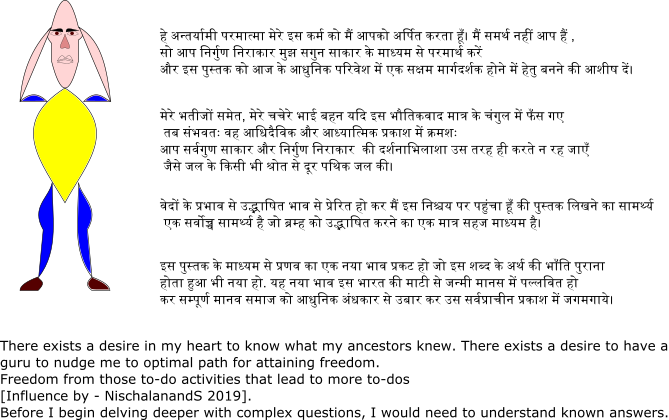
\includegraphics{comic_strips/Preface}
%%LaTeX with PSTricks extensions
%%Creator: Inkscape 1.0 (4035a4f, 2020-05-01)
%%Please note this file requires PSTricks extensions
\psset{xunit=.5pt,yunit=.5pt,runit=.5pt}
\begin{pspicture}(453.54330709,559.37007874)
{
\newrgbcolor{curcolor}{1 0.83529413 0.83529413}
\pscustom[linestyle=none,fillstyle=solid,fillcolor=curcolor]
{
\newpath
\moveto(59.48863748,498.71142425)
\curveto(65.52978142,530.90664227)(71.73993449,534.6689983)(78.18618709,498.71142425)
\curveto(82.85345008,493.77488504)(81.80056441,489.98327811)(78.18618709,486.70436787)
\lineto(78.18618709,466.74458835)
\curveto(71.73993449,430.78701732)(65.52978142,434.54937449)(59.48863748,466.74458835)
\lineto(59.48863748,483.58564913)
\curveto(54.45992315,491.3955515)(56.29635024,495.42664441)(59.48863748,498.71142425)
\closepath
}
}
{
\newrgbcolor{curcolor}{0 0 0}
\pscustom[linewidth=0.44635464,linecolor=curcolor]
{
\newpath
\moveto(59.48863748,498.71142425)
\curveto(65.52978142,530.90664227)(71.73993449,534.6689983)(78.18618709,498.71142425)
\curveto(82.85345008,493.77488504)(81.80056441,489.98327811)(78.18618709,486.70436787)
\lineto(78.18618709,466.74458835)
\curveto(71.73993449,430.78701732)(65.52978142,434.54937449)(59.48863748,466.74458835)
\lineto(59.48863748,483.58564913)
\curveto(54.45992315,491.3955515)(56.29635024,495.42664441)(59.48863748,498.71142425)
\closepath
}
}
{
\newrgbcolor{curcolor}{0 0 0}
\pscustom[linewidth=0.44635464,linecolor=curcolor]
{
\newpath
\moveto(68.83741228,441.17111811)
\curveto(28.70297726,406.66343811)(53.1872126,369.38420409)(68.83741228,332.48386772)
\curveto(82.5847748,368.3198589)(110.20004787,403.75930961)(68.83741228,441.17111811)
\closepath
}
}
{
\newrgbcolor{curcolor}{0 0 0}
\pscustom[linewidth=0.44635464,linecolor=curcolor]
{
\newpath
\moveto(78.18618709,351.66397228)
\curveto(80.36249575,336.80646047)(93.4629052,328.62201449)(84.4187074,306.91038992)
\lineto(87.53496567,262.1568189)
\curveto(73.00332472,287.5683137)(78.42004913,320.71113449)(78.18618709,351.66397228)
\closepath
}
}
{
\newrgbcolor{curcolor}{0 0 1}
\pscustom[linestyle=none,fillstyle=solid,fillcolor=curcolor]
{
\newpath
\moveto(59.99251654,351.66397228)
\curveto(57.81621165,336.80645669)(44.71579465,328.62201449)(53.76,306.91038992)
\lineto(50.64374173,262.15677732)
\curveto(65.17537512,287.56826457)(59.75865071,320.71113827)(59.99251654,351.66397228)
\closepath
}
}
{
\newrgbcolor{curcolor}{0 0 0}
\pscustom[linewidth=0.44635464,linecolor=curcolor]
{
\newpath
\moveto(59.99251654,351.66397228)
\curveto(57.81621165,336.80645669)(44.71579465,328.62201449)(53.76,306.91038992)
\lineto(50.64374173,262.15677732)
\curveto(65.17537512,287.56826457)(59.75865071,320.71113827)(59.99251654,351.66397228)
\closepath
}
}
{
\newrgbcolor{curcolor}{1 0.83529413 0.83529413}
\pscustom[linestyle=none,fillstyle=solid,fillcolor=curcolor]
{
\newpath
\moveto(56.37237921,428.38438299)
\curveto(49.69209071,437.80056189)(43.54634457,435.97589291)(37.67482809,428.38438299)
\curveto(38.94881386,454.41614362)(44.91686173,478.42117417)(59.48863748,498.71142425)
\lineto(37.67482809,428.38438299)
\closepath
}
}
{
\newrgbcolor{curcolor}{0 0 0}
\pscustom[linewidth=0.44635464,linecolor=curcolor]
{
\newpath
\moveto(56.37237921,428.38438299)
\curveto(49.69209071,437.80056189)(43.54634457,435.97589291)(37.67482809,428.38438299)
\curveto(38.94881386,454.41614362)(44.91686173,478.42117417)(59.48863748,498.71142425)
\lineto(37.67482809,428.38438299)
\closepath
}
}
{
\newrgbcolor{curcolor}{1 0.83529413 0.83529413}
\pscustom[linestyle=none,fillstyle=solid,fillcolor=curcolor]
{
\newpath
\moveto(81.77331024,428.38438299)
\lineto(100.47086362,428.38438299)
\curveto(98.01121512,457.10265827)(95.10084283,485.3267074)(78.65705197,498.71142425)
\lineto(100.47086362,428.38438299)
\curveto(95.08862362,431.96048882)(90.9548485,440.78740535)(81.77331024,428.38438299)
\closepath
}
}
{
\newrgbcolor{curcolor}{0 0 0}
\pscustom[linewidth=0.44635464,linecolor=curcolor]
{
\newpath
\moveto(81.77331024,428.38438299)
\lineto(100.47086362,428.38438299)
\curveto(98.01121512,457.10265827)(95.10084283,485.3267074)(78.65705197,498.71142425)
\lineto(100.47086362,428.38438299)
\curveto(95.08862362,431.96048882)(90.9548485,440.78740535)(81.77331024,428.38438299)
\closepath
}
}
{
\newrgbcolor{curcolor}{0.33333334 0 0}
\pscustom[linestyle=none,fillstyle=solid,fillcolor=curcolor]
{
\newpath
\moveto(50.13986268,262.1568189)
\curveto(50.96890205,258.47535118)(56.74524472,258.25974047)(50.13986268,249.37008)
\lineto(37.67482809,249.37008)
\curveto(37.70563124,253.59144189)(41.71858772,257.8522885)(50.13986268,262.1568189)
\closepath
}
}
{
\newrgbcolor{curcolor}{0 0 0}
\pscustom[linewidth=0.44635464,linecolor=curcolor]
{
\newpath
\moveto(50.13986268,262.1568189)
\curveto(50.96890205,258.47535118)(56.74524472,258.25974047)(50.13986268,249.37008)
\lineto(37.67482809,249.37008)
\curveto(37.70563124,253.59144189)(41.71858772,257.8522885)(50.13986268,262.1568189)
\closepath
}
}
{
\newrgbcolor{curcolor}{0 0 0}
\pscustom[linewidth=0.44635464,linecolor=curcolor]
{
\newpath
\moveto(87.53496567,262.1568189)
\curveto(84.64321134,258.47337071)(82.26852283,254.68645417)(87.53496567,249.37008)
\lineto(99.99999874,249.37008)
\curveto(99.74053417,253.34300976)(96.72232441,257.52085417)(87.53496567,262.1568189)
\closepath
}
}
{
\newrgbcolor{curcolor}{1 1 0}
\pscustom[linestyle=none,fillstyle=solid,fillcolor=curcolor]
{
\newpath
\moveto(62.94664063,346.90422425)
\curveto(53.79528945,367.63863685)(51.34846866,374.19887622)(49.11628724,383.98522583)
\curveto(44.46639874,404.37130205)(49.21168252,420.61678488)(64.31306835,436.01136378)
\lineto(68.63782299,440.42008063)
\lineto(71.1536315,438.1049537)
\curveto(79.00998047,430.87530709)(86.26734992,419.26529386)(88.71171024,410.01635906)
\curveto(89.93321953,405.39440504)(90.01079811,404.65501228)(90.01079811,397.63512945)
\curveto(90.01079811,390.42292913)(89.9564485,389.94633449)(88.41084094,383.60090835)
\curveto(86.34765732,375.13069984)(83.74243276,368.11116094)(76.6635137,351.94875591)
\curveto(73.50284976,344.73242079)(70.42459465,337.69748031)(69.82294299,336.31553764)
\lineto(68.72903055,333.80294173)
\closepath
}
}
{
\newrgbcolor{curcolor}{0 0 1}
\pscustom[linestyle=none,fillstyle=solid,fillcolor=curcolor]
{
\newpath
\moveto(84.58468535,269.4681789)
\curveto(80.81544567,278.14445102)(78.49749165,290.27391874)(77.83688315,304.77836598)
\curveto(77.69375244,307.9209789)(77.79579969,318.85505386)(78.06320126,329.07630992)
\lineto(78.54977008,347.66041701)
\lineto(79.56929386,344.8036422)
\curveto(80.13003213,343.23241323)(81.71467465,339.38410205)(83.09072126,336.25184126)
\curveto(84.46676409,333.11957669)(85.9454022,329.06167937)(86.37658961,327.23428535)
\curveto(87.70702866,321.59577449)(87.25626709,315.79031811)(85.02123969,309.77852976)
\lineto(84.04553197,307.15406362)
\lineto(85.45107024,286.97015055)
\curveto(86.22411213,275.86900157)(86.7888189,266.36903811)(86.70596787,265.85911937)
\curveto(86.62312063,265.34919685)(85.66854047,266.97327874)(84.58468157,269.4681789)
\closepath
}
}
{
\newrgbcolor{curcolor}{0 0 1}
\pscustom[linestyle=none,fillstyle=solid,fillcolor=curcolor]
{
\newpath
\moveto(83.36024693,429.31474394)
\curveto(83.36024693,430.04021669)(86.48859591,432.63862677)(88.44497764,433.53812787)
\curveto(90.69739087,434.5737411)(93.36407433,433.69505386)(96.29617512,430.95101858)
\lineto(98.37149102,429.00882898)
\lineto(90.86587465,428.94491717)
\curveto(86.73778016,428.90976756)(83.36024693,429.07621795)(83.36024693,429.31470614)
\closepath
}
}
{
\newrgbcolor{curcolor}{0 0 1}
\pscustom[linestyle=none,fillstyle=solid,fillcolor=curcolor]
{
\newpath
\moveto(41.03624693,430.90446992)
\curveto(43.7872252,433.57608945)(46.80863622,434.58869291)(49.25241827,433.65805606)
\curveto(51.24413858,432.89956913)(54.85788472,430.08912)(54.85788472,429.29861291)
\curveto(54.85788472,429.06893102)(51.30933543,428.91030425)(46.97222929,428.94605858)
\lineto(39.08657386,429.01106646)
\closepath
}
}
{
\newrgbcolor{curcolor}{0.33333334 0 0}
\pscustom[linestyle=none,fillstyle=solid,fillcolor=curcolor]
{
\newpath
\moveto(86.04963024,252.35308724)
\curveto(84.52642394,254.98262173)(84.57327496,256.79178331)(86.23180346,259.38710929)
\lineto(87.58322268,261.50187591)
\lineto(91.04209512,259.37764913)
\curveto(94.97661732,256.96129134)(97.66052787,254.37318803)(98.71542047,251.9782148)
\lineto(99.43937008,250.33458142)
\lineto(93.32912126,250.33458142)
\curveto(87.31002709,250.33458142)(87.20142992,250.36443969)(86.04963024,252.35308724)
\closepath
}
}
{
\newrgbcolor{curcolor}{0 0 0}
\pscustom[linewidth=0.14369461,linecolor=curcolor]
{
\newpath
\moveto(58.77593197,492.31804724)
\curveto(61.72621984,496.95135118)(64.24953827,496.08872693)(66.61786583,492.31804724)
\curveto(63.53999244,489.76359685)(61.09712882,490.70589354)(58.77593197,492.31804724)
\closepath
}
}
{
\newrgbcolor{curcolor}{0 0 0}
\pscustom[linestyle=none,fillstyle=solid,fillcolor=curcolor]
{
\newpath
\moveto(58.25314016,495.79368567)
\lineto(67.4020611,494.21385071)
\curveto(67.70355402,500.50810961)(61.62329953,495.8187326)(58.25314016,495.79368567)
\closepath
}
}
{
\newrgbcolor{curcolor}{0 0 0}
\pscustom[linewidth=0.14369461,linecolor=curcolor]
{
\newpath
\moveto(58.25314016,495.79368567)
\lineto(67.4020611,494.21385071)
\curveto(67.70355402,500.50810961)(61.62329953,495.8187326)(58.25314016,495.79368567)
\closepath
}
}
{
\newrgbcolor{curcolor}{0.33333334 0 0}
\pscustom[linestyle=none,fillstyle=solid,fillcolor=curcolor]
{
\newpath
\moveto(64.52668246,492.9499901)
\curveto(64.52668246,494.35756917)(63.11887416,495.06223227)(62.29555952,494.06704421)
\curveto(61.47224489,493.07185616)(62.05520952,491.37015677)(63.2196934,491.37015677)
\curveto(64.38417728,491.37015677)(64.96714192,493.07185616)(64.14382728,494.06704421)
\curveto(63.32051265,495.06223227)(61.91270434,494.35756917)(61.91270434,492.9499901)
\curveto(61.91270434,491.54241103)(63.32051265,490.83774793)(64.14382728,491.83293599)
\curveto(64.96714192,492.82812404)(64.38417728,494.52982343)(63.2196934,494.52982343)
\curveto(62.05520952,494.52982343)(61.47224489,492.82812404)(62.29555952,491.83293599)
\curveto(63.11887416,490.83774793)(64.52668246,491.54241103)(64.52668246,492.9499901)
\closepath
}
}
{
\newrgbcolor{curcolor}{0 0 0}
\pscustom[linewidth=0.14369461,linecolor=curcolor]
{
\newpath
\moveto(78.18619087,492.3180548)
\curveto(75.23589165,496.95135496)(72.71256945,496.08873071)(70.34424945,492.3180548)
\curveto(73.42211906,489.76360063)(75.8649789,490.70589732)(78.18619087,492.3180548)
\closepath
}
}
{
\newrgbcolor{curcolor}{0 0 0}
\pscustom[linestyle=none,fillstyle=solid,fillcolor=curcolor]
{
\newpath
\moveto(78.70896756,495.79368945)
\lineto(69.56005039,494.21385449)
\curveto(69.25859528,500.50811339)(75.33880441,495.81874016)(78.70896756,495.79368945)
\closepath
}
}
{
\newrgbcolor{curcolor}{0 0 0}
\pscustom[linewidth=0.14369461,linecolor=curcolor]
{
\newpath
\moveto(78.70896756,495.79368945)
\lineto(69.56005039,494.21385449)
\curveto(69.25859528,500.50811339)(75.33880441,495.81874016)(78.70896756,495.79368945)
\closepath
}
}
{
\newrgbcolor{curcolor}{0.33333334 0 0}
\pscustom[linestyle=none,fillstyle=solid,fillcolor=curcolor]
{
\newpath
\moveto(72.43535031,492.95000452)
\curveto(72.43535031,492.07748666)(73.02050924,491.37017119)(73.74233937,491.37017119)
\curveto(74.46416949,491.37017119)(75.04932843,492.07748666)(75.04932843,492.95000452)
\curveto(75.04932843,493.82252237)(74.46416949,494.52983785)(73.74233937,494.52983785)
\curveto(73.02050924,494.52983785)(72.43535031,493.82252237)(72.43535031,492.95000452)
}
}
{
\newrgbcolor{curcolor}{0.87058824 0.52941179 0.52941179}
\pscustom[linestyle=none,fillstyle=solid,fillcolor=curcolor]
{
\newpath
\moveto(68.83741984,492.3180548)
\curveto(68.44427339,487.61012787)(61.68030992,475.68023433)(68.83741984,479.53131969)
\curveto(75.78075591,475.24404283)(69.44821795,487.30371402)(68.83741984,492.3180548)
\closepath
}
}
{
\newrgbcolor{curcolor}{0 0 0}
\pscustom[linewidth=0.20200668,linecolor=curcolor]
{
\newpath
\moveto(68.83741984,492.3180548)
\curveto(68.44427339,487.61012787)(61.68030992,475.68023433)(68.83741984,479.53131969)
\curveto(75.78075591,475.24404283)(69.44821795,487.30371402)(68.83741984,492.3180548)
\closepath
}
}
{
\newrgbcolor{curcolor}{0 0 0}
\pscustom[linewidth=0.18197177,linecolor=curcolor]
{
\newpath
\moveto(63.53977323,466.74458835)
\curveto(66.65602772,475.2455622)(67.95708472,470.7819515)(68.73270425,469.95626835)
\curveto(70.10470299,468.49568504)(71.33041512,477.37080189)(74.44666961,466.74458835)
\curveto(71.16975496,470.23426772)(66.58010835,468.89877543)(63.53977323,466.74458835)
\closepath
}
}
{
\newrgbcolor{curcolor}{0 0 0}
\pscustom[linewidth=0.18197177,linecolor=curcolor]
{
\newpath
\moveto(63.53977323,465.68196661)
\curveto(67.67789102,469.01673827)(71.15621669,467.9728252)(74.44666961,465.68196661)
\curveto(71.61315024,464.06078362)(67.76862614,464.48297575)(63.53977323,465.68196661)
\closepath
}
}
{
\newrgbcolor{curcolor}{0 0 0}
\pscustom[linestyle=none,fillstyle=solid,fillcolor=curcolor]
{
\newpath
\moveto(139.78288022,516.05425966)
\lineto(139.78288022,515.17787124)
\lineto(138.50246767,515.17787124)
\lineto(138.61518004,512.85112173)
\lineto(136.10845686,512.85112173)
\curveto(135.93112273,512.85112173)(135.79737071,512.81820573)(135.70720082,512.75237374)
\curveto(135.62003658,512.68654174)(135.57645446,512.589851)(135.57645446,512.46230152)
\curveto(135.57645446,512.30595053)(135.62604791,512.12079805)(135.7252348,511.90684407)
\curveto(135.82442168,511.69700459)(135.97320202,511.46042087)(136.17157579,511.19709289)
\curveto(136.5232384,511.50568036)(136.92449444,511.6599741)(137.37534394,511.6599741)
\curveto(137.78711981,511.6599741)(138.1477994,511.45630637)(138.45738272,511.04897091)
\curveto(138.76696603,510.64163545)(138.92175769,510.20344124)(138.92175769,509.73438829)
\curveto(138.92175769,509.39288482)(138.85112461,509.06166761)(138.70985843,508.74073664)
\curveto(138.57159792,508.41980567)(138.36270432,508.10504645)(138.08317764,507.79645898)
\lineto(137.56470072,508.49386666)
\curveto(137.910352,508.81068313)(138.16883904,509.10075535)(138.34016185,509.36408333)
\curveto(138.51449032,509.6274113)(138.60165455,509.86399503)(138.60165455,510.07383451)
\curveto(138.60165455,510.31658998)(138.53102147,510.51408596)(138.38975529,510.66632245)
\curveto(138.24848912,510.82267343)(138.06364083,510.90084892)(137.83521042,510.90084892)
\curveto(137.39938924,510.90084892)(136.9891162,510.73009719)(136.60439131,510.38859372)
\curveto(136.21966641,510.05120476)(136.02730396,509.6232968)(136.02730396,509.10486985)
\curveto(136.02730396,508.50826741)(136.34590426,507.88903522)(136.98310488,507.24717329)
\curveto(137.30170519,506.92624232)(137.67891593,506.62999835)(138.1147371,506.35844138)
\curveto(138.55356394,506.08688441)(139.04949838,505.84001443)(139.60254043,505.61783145)
\lineto(139.54392999,505.35861798)
\lineto(139.21480986,505.50673996)
\curveto(138.11173144,506.00459441)(137.19500414,506.6238266)(136.46462796,507.36443653)
\curveto(136.09793704,507.73474149)(135.82291885,508.10093195)(135.63957339,508.46300792)
\curveto(135.4592336,508.82919838)(135.3690637,509.19538884)(135.3690637,509.56157931)
\curveto(135.3690637,510.07177726)(135.5779573,510.55934546)(135.99574449,511.02428391)
\curveto(135.41565148,511.84718383)(135.12560497,512.48287401)(135.12560497,512.93135447)
\curveto(135.12560497,513.22348394)(135.19924372,513.42920892)(135.34652122,513.54852941)
\curveto(135.49680439,513.6678499)(135.75078293,513.72751014)(136.10845686,513.72751014)
\lineto(137.96144828,513.72751014)
\lineto(137.96144828,515.17787124)
\lineto(134.61163655,515.17787124)
\lineto(134.61163655,516.05425966)
\closepath
\moveto(138.53402713,516.05425966)
\closepath
\moveto(137.79463396,505.58697271)
\closepath
}
}
{
\newrgbcolor{curcolor}{0 0 0}
\pscustom[linestyle=none,fillstyle=solid,fillcolor=curcolor]
{
\newpath
\moveto(135.14363881,518.55381816)
\lineto(134.85509514,519.60301555)
\lineto(135.31947011,519.60301555)
\curveto(135.58396848,519.60301555)(135.8364442,519.54129806)(136.07689726,519.41786307)
\curveto(136.31434466,519.29854258)(136.53225525,519.1216191)(136.73062902,518.88709262)
\curveto(136.92599713,518.65256615)(137.18147851,518.24111619)(137.49707316,517.65274275)
\lineto(138.42582311,515.92465292)
\lineto(138.14629643,515.92465292)
\lineto(137.38436078,517.28243778)
\curveto(137.13489073,517.72680374)(136.88992918,518.04979196)(136.64947611,518.25140244)
\curveto(136.40601739,518.45301292)(136.10845672,518.55381816)(135.75679412,518.55381816)
\closepath
\moveto(138.53402699,516.05425966)
\closepath
}
}
{
\newrgbcolor{curcolor}{0 0 0}
\pscustom[linestyle=none,fillstyle=solid,fillcolor=curcolor]
{
\newpath
\moveto(148.75027704,516.05425966)
\lineto(148.75027704,515.17787124)
\lineto(147.37969459,515.17787124)
\lineto(147.37969459,508.15442045)
\lineto(147.1903378,508.15442045)
\lineto(146.67186088,508.99377836)
\lineto(146.67186088,511.77106559)
\curveto(146.34123792,511.6188291)(146.01512346,511.55916886)(145.69351749,511.59208485)
\curveto(145.7085458,511.47687887)(145.71605996,511.36373013)(145.71605996,511.25263864)
\curveto(145.71605996,510.77535669)(145.60034192,510.38653647)(145.36890585,510.086178)
\curveto(145.14047544,509.78993403)(144.84291478,509.64181205)(144.47622386,509.64181205)
\curveto(144.00132906,509.64181205)(143.59255885,509.93188427)(143.24991324,510.51202871)
\curveto(142.90726763,511.09628765)(142.69837403,511.78546633)(142.62323245,512.57956475)
\lineto(142.84865719,512.57956475)
\curveto(142.92680444,511.97884781)(143.09963008,511.48099336)(143.36713411,511.0860014)
\curveto(143.6376438,510.69100944)(143.94121579,510.49351346)(144.27785008,510.49351346)
\curveto(144.4972635,510.49351346)(144.7016486,510.59226145)(144.89100539,510.78975743)
\curveto(145.08036218,510.98725341)(145.17504057,511.26086764)(145.17504057,511.6106001)
\curveto(145.17504057,511.80809608)(145.12995562,511.99530581)(145.03978572,512.1722293)
\curveto(144.94961582,512.35326728)(144.81736664,512.48698851)(144.64303817,512.57339301)
\curveto(144.47171536,512.663912)(144.33044919,512.70917149)(144.21923965,512.70917149)
\curveto(144.10502444,512.70917149)(143.93520447,512.67625549)(143.70977972,512.6104235)
\lineto(143.20482829,513.41892267)
\curveto(143.75787033,513.47652566)(144.2027085,513.6267049)(144.53934279,513.86946038)
\curveto(144.87597707,514.11633035)(145.04429422,514.41257432)(145.04429422,514.75819229)
\curveto(145.04429422,514.97626076)(144.97516396,515.15729875)(144.83690345,515.30130623)
\curveto(144.7016486,515.44531372)(144.53783996,515.51731746)(144.34547751,515.51731746)
\curveto(144.00583755,515.51731746)(143.56550788,515.31364973)(143.02448849,514.90631427)
\lineto(142.62323245,515.69629819)
\curveto(143.0530423,515.93493917)(143.466321,516.05425966)(143.86306855,516.05425966)
\curveto(144.32594069,516.05425966)(144.69864294,515.89379417)(144.98117529,515.5728632)
\curveto(145.2667133,515.25604674)(145.40948231,514.83431053)(145.40948231,514.30765458)
\curveto(145.40948231,514.00318161)(145.33884922,513.73779639)(145.19758305,513.51149891)
\curveto(145.05631687,513.28520143)(144.84441761,513.0979917)(144.56188526,512.94986972)
\curveto(145.05481404,512.63716775)(145.46358425,512.48081676)(145.78819588,512.48081676)
\curveto(146.37730588,512.48081676)(146.67186088,512.87375148)(146.67186088,513.6596209)
\lineto(146.67186088,515.17787124)
\lineto(145.98656966,515.17787124)
\lineto(145.48161823,516.05425966)
\closepath
\moveto(147.37969459,516.05425966)
\closepath
}
}
{
\newrgbcolor{curcolor}{0 0 0}
\pscustom[linestyle=none,fillstyle=solid,fillcolor=curcolor]
{
\newpath
\moveto(151.84761228,515.17787124)
\lineto(148.62403841,515.17787124)
\lineto(148.62403841,516.05425966)
\lineto(151.84761228,516.05425966)
\closepath
\moveto(151.96483314,512.44995802)
\lineto(150.62130166,512.44995802)
\curveto(150.40789957,512.44995802)(150.27715321,512.39441227)(150.2290626,512.28332078)
\curveto(150.18397765,512.1763438)(150.16143518,511.95210357)(150.16143518,511.6106001)
\curveto(150.16143518,511.43779112)(150.171955,511.24646689)(150.19299464,511.03662741)
\curveto(150.20201163,510.91730692)(150.20652013,510.78975743)(150.20652013,510.65397895)
\curveto(150.20652013,510.46882647)(150.14941252,510.37625023)(150.03519732,510.37625023)
\curveto(149.89994247,510.37625023)(149.6970602,510.6560362)(149.4265505,511.21560814)
\curveto(149.15904647,511.77518009)(149.02529446,512.21954604)(149.02529446,512.54870601)
\curveto(149.02529446,512.77911798)(149.08089923,512.96427047)(149.19210877,513.10416345)
\curveto(149.30331831,513.24817094)(149.43256183,513.32017468)(149.57983933,513.32017468)
\lineto(151.96483314,513.32017468)
\closepath
\moveto(152.08205401,508.42597742)
\closepath
\moveto(154.0432493,508.42597742)
\closepath
}
}
{
\newrgbcolor{curcolor}{0 0 0}
\pscustom[linestyle=none,fillstyle=solid,fillcolor=curcolor]
{
\newpath
\moveto(157.26231499,516.05425966)
\lineto(157.26231499,515.17787124)
\lineto(155.89173254,515.17787124)
\lineto(155.89173254,508.15442045)
\lineto(155.67983328,508.15442045)
\lineto(155.18389884,508.94440437)
\lineto(155.18389884,512.83877823)
\lineto(154.0657921,512.83877823)
\curveto(153.58488597,512.83877823)(153.24975451,512.72974399)(153.06039773,512.51167551)
\curveto(152.87104094,512.29360703)(152.77636255,511.99324856)(152.77636255,511.6106001)
\curveto(152.77636255,511.20326464)(152.89658908,510.76095594)(153.13704214,510.28367398)
\curveto(153.38050087,509.80639203)(153.77574559,509.18304535)(154.32277631,508.41363392)
\lineto(154.16948748,508.21613794)
\curveto(153.40905467,509.23653384)(152.91011456,510.01623151)(152.67266717,510.55523096)
\curveto(152.43521977,511.0942304)(152.31649607,511.6352871)(152.31649607,512.17840104)
\curveto(152.31649607,512.639225)(152.41117446,513.00952996)(152.60053125,513.28931593)
\curveto(152.78988803,513.56910191)(153.1160025,513.70899489)(153.57887464,513.70899489)
\lineto(155.18389884,513.70899489)
\lineto(155.18389884,515.17787124)
\lineto(151.72588323,515.17787124)
\lineto(151.72588323,516.05425966)
\closepath
\moveto(155.89173254,508.36425993)
\closepath
\moveto(155.89173254,516.05425966)
\closepath
}
}
{
\newrgbcolor{curcolor}{0 0 0}
\pscustom[linestyle=none,fillstyle=solid,fillcolor=curcolor]
{
\newpath
\moveto(162.80776387,516.05425966)
\lineto(162.80776387,515.17787124)
\lineto(161.43718141,515.17787124)
\lineto(161.43718141,508.15442045)
\lineto(161.34250302,508.15442045)
\lineto(160.72934771,508.99377836)
\lineto(160.72934771,510.77124219)
\curveto(160.45883802,510.47088372)(160.11769523,510.32070448)(159.70591937,510.32070448)
\curveto(159.4083587,510.32070448)(159.10328388,510.46265472)(158.7906949,510.74655519)
\curveto(158.48111158,511.03045566)(158.06182155,511.57974135)(157.53282481,512.39441227)
\lineto(157.53282481,512.51784726)
\curveto(158.00170829,512.57545025)(158.35337089,512.74208749)(158.58781263,513.01775896)
\curveto(158.82225436,513.29754493)(158.93947523,513.68430789)(158.93947523,514.17804784)
\curveto(158.93947523,514.56892531)(158.83427701,514.90219977)(158.62388058,515.17787124)
\lineto(157.13607726,515.17787124)
\lineto(157.13607726,516.05425966)
\closepath
\moveto(160.72934771,515.17787124)
\lineto(158.89439028,515.17787124)
\curveto(159.32420013,514.77465028)(159.53910505,514.27679583)(159.53910505,513.68430789)
\curveto(159.53910505,513.19879694)(159.42789551,512.79763323)(159.20547643,512.48081676)
\curveto(158.98606301,512.1681148)(158.65544005,511.94181732)(158.21360755,511.80192433)
\curveto(158.42700964,511.53448186)(158.62688625,511.33492863)(158.81323737,511.20326464)
\curveto(159.00259416,511.07160066)(159.17992829,511.00576866)(159.34523977,511.00576866)
\curveto(159.6458061,511.00576866)(159.92082429,511.1189174)(160.17029434,511.34521488)
\curveto(160.42277006,511.57151236)(160.57906455,511.77723734)(160.63917781,511.96238982)
\curveto(160.69929108,512.1475423)(160.72934771,512.50756101)(160.72934771,513.04244596)
\closepath
\moveto(161.43718141,508.36425993)
\closepath
\moveto(161.43718141,516.05425966)
\closepath
}
}
{
\newrgbcolor{curcolor}{0 0 0}
\pscustom[linestyle=none,fillstyle=solid,fillcolor=curcolor]
{
\newpath
\moveto(165.75181112,516.05425966)
\lineto(165.75181112,515.17787124)
\lineto(164.38573716,515.17787124)
\lineto(164.38573716,508.15442045)
\lineto(164.21892285,508.15442045)
\lineto(163.67790346,509.01229361)
\lineto(163.67790346,515.17787124)
\lineto(162.67250909,515.17787124)
\lineto(162.67250909,516.05425966)
\closepath
\moveto(164.38573716,516.05425966)
\closepath
}
}
{
\newrgbcolor{curcolor}{0 0 0}
\pscustom[linestyle=none,fillstyle=solid,fillcolor=curcolor]
{
\newpath
\moveto(165.50835234,518.37483742)
\lineto(165.35506351,518.15265445)
\curveto(164.91623667,518.6463944)(164.55104859,518.89326437)(164.25949925,518.89326437)
\curveto(164.02205185,518.89326437)(163.82367807,518.78423013)(163.66437792,518.56616165)
\curveto(163.5020721,518.34809318)(163.42091919,518.09093695)(163.42091919,517.79469298)
\curveto(163.42091919,517.57251)(163.50357493,517.30506753)(163.66888641,516.99236556)
\curveto(163.83119223,516.67966359)(164.07465096,516.32375938)(164.39926259,515.92465292)
\lineto(164.09268494,515.92465292)
\curveto(163.69293172,516.30730138)(163.39236539,516.69200709)(163.19098595,517.07877005)
\curveto(162.98960651,517.46553301)(162.88891679,517.85641048)(162.88891679,518.25140244)
\curveto(162.88891679,518.6463944)(162.98209235,518.97349711)(163.16844348,519.23271059)
\curveto(163.35178894,519.49192406)(163.61328164,519.6215308)(163.95292159,519.6215308)
\curveto(164.19638032,519.6215308)(164.43232489,519.53718356)(164.66075529,519.36848907)
\curveto(164.8891857,519.20390909)(165.17171805,518.87269187)(165.50835234,518.37483742)
\closepath
\moveto(164.3857371,516.05425966)
\closepath
}
}
{
\newrgbcolor{curcolor}{0 0 0}
\pscustom[linestyle=none,fillstyle=solid,fillcolor=curcolor]
{
\newpath
\moveto(171.60383747,516.05425966)
\lineto(171.60383747,515.17787124)
\lineto(170.23325501,515.17787124)
\lineto(170.23325501,508.15442045)
\lineto(170.03037274,508.15442045)
\lineto(169.52542131,508.96291962)
\lineto(169.52542131,511.45013462)
\lineto(167.6724299,511.45013462)
\lineto(167.6724299,510.40093722)
\curveto(167.6724299,510.15406725)(167.61381947,510.03063226)(167.4965986,510.03063226)
\curveto(167.38238339,510.03063226)(167.12089069,510.32893348)(166.71212048,510.92553592)
\curveto(166.30635594,511.52625286)(166.10347367,511.92741657)(166.10347367,512.12902705)
\curveto(166.10347367,512.25657654)(166.17410676,512.32035128)(166.31537293,512.32035128)
\lineto(166.9645962,512.32035128)
\lineto(166.9645962,515.17787124)
\lineto(165.6300817,515.17787124)
\lineto(165.6300817,516.05425966)
\closepath
\moveto(167.6724299,512.32035128)
\lineto(169.52542131,512.32035128)
\lineto(169.52542131,515.17787124)
\lineto(167.6724299,515.17787124)
\closepath
\moveto(170.23325501,508.36425993)
\closepath
\moveto(170.23325501,516.05425966)
\closepath
}
}
{
\newrgbcolor{curcolor}{0 0 0}
\pscustom[linestyle=none,fillstyle=solid,fillcolor=curcolor]
{
\newpath
\moveto(174.55239439,516.05425966)
\lineto(174.55239439,515.17787124)
\lineto(173.18632043,515.17787124)
\lineto(173.18632043,508.1729357)
\lineto(172.98343816,508.1729357)
\lineto(172.47848673,508.96291962)
\lineto(172.47848673,515.17787124)
\lineto(171.47309236,515.17787124)
\lineto(171.47309236,516.05425966)
\lineto(172.92482773,516.05425966)
\curveto(172.62125574,516.98002206)(172.29514127,517.67537249)(171.94648433,518.14031095)
\curveto(171.59782739,518.6052494)(171.22662797,518.83771863)(170.83288608,518.83771863)
\curveto(170.50526879,518.83771863)(170.2588044,518.71428364)(170.09349292,518.46741366)
\curveto(169.92818144,518.22054369)(169.8455257,517.85023873)(169.8455257,517.35649878)
\curveto(169.8455257,516.94093432)(169.91315312,516.50685461)(170.04840797,516.05425966)
\lineto(169.50738858,516.05425966)
\curveto(169.26092419,516.56445761)(169.13769199,517.1013998)(169.13769199,517.66508624)
\curveto(169.13769199,518.25345969)(169.27895817,518.73485614)(169.56149052,519.1092756)
\curveto(169.8410172,519.48369506)(170.1971883,519.67090479)(170.63000381,519.67090479)
\curveto(171.29726106,519.67090479)(171.85932009,519.27591283)(172.31618091,518.48592891)
\curveto(172.63778688,517.93047147)(172.92783339,517.11991505)(173.18632043,516.05425966)
\closepath
}
}
{
\newrgbcolor{curcolor}{0 0 0}
\pscustom[linestyle=none,fillstyle=solid,fillcolor=curcolor]
{
\newpath
\moveto(182.33856475,516.05425966)
\lineto(182.33856475,515.17787124)
\lineto(180.9679823,515.17787124)
\lineto(180.9679823,508.15442045)
\lineto(180.792151,508.15442045)
\lineto(180.2601486,508.97526312)
\lineto(180.2601486,511.46247812)
\curveto(180.03472385,511.19503564)(179.76421416,511.06131441)(179.44861951,511.06131441)
\curveto(179.17810982,511.06131441)(178.90910295,511.1682914)(178.64159892,511.38224537)
\curveto(178.37409489,511.59619935)(178.14416165,511.85129833)(177.9517992,512.1475423)
\curveto(177.76244241,512.44790077)(177.66776402,512.81203398)(177.66776402,513.23994194)
\lineto(177.66776402,515.17787124)
\lineto(176.99148978,515.17787124)
\lineto(176.99148978,516.05425966)
\closepath
\moveto(180.2601486,515.17787124)
\lineto(178.37559772,515.17787124)
\lineto(178.37559772,512.77088899)
\curveto(178.37559772,512.23188954)(178.44923647,511.89244332)(178.59651397,511.75255034)
\curveto(178.74379147,511.61677185)(178.91661711,511.54888261)(179.11499089,511.54888261)
\curveto(179.46965915,511.54888261)(179.85137839,511.86569908)(180.2601486,512.49933201)
\closepath
\moveto(180.9679823,508.36425993)
\closepath
\moveto(180.9679823,516.05425966)
\closepath
}
}
{
\newrgbcolor{curcolor}{0 0 0}
\pscustom[linestyle=none,fillstyle=solid,fillcolor=curcolor]
{
\newpath
\moveto(186.82000716,516.05425966)
\lineto(186.82000716,515.17787124)
\lineto(184.81372692,515.17787124)
\curveto(184.9219308,514.80345178)(184.97603274,514.38377282)(184.97603274,513.91883437)
\curveto(184.97603274,513.40863642)(184.893377,512.92723997)(184.72806552,512.47464502)
\curveto(184.5657597,512.02616456)(184.32230098,511.60854285)(183.99768934,511.22177989)
\curveto(184.27721603,510.79798643)(184.61986164,510.35156323)(185.02562618,509.88251028)
\curveto(185.43439639,509.41757182)(185.90628552,508.92794637)(186.44129359,508.41363392)
\lineto(186.32407272,508.1852792)
\curveto(185.85218359,508.62964515)(185.41786524,509.06989661)(185.02111769,509.50603356)
\curveto(184.62437014,509.94628502)(184.26369054,510.38242197)(183.93907891,510.81444443)
\curveto(183.2928613,511.68260384)(182.9697525,512.30800778)(182.9697525,512.69065624)
\curveto(182.9697525,513.06919021)(183.15460079,513.25845719)(183.52429738,513.25845719)
\curveto(183.70163151,513.25845719)(183.9150336,513.20496869)(184.16450365,513.0979917)
\curveto(184.35386044,513.43126617)(184.44853883,513.77071239)(184.44853883,514.11633035)
\curveto(184.44853883,514.38788732)(184.38091141,514.74173429)(184.24565656,515.17787124)
\lineto(182.20330836,515.17787124)
\lineto(182.20330836,516.05425966)
\closepath
\moveto(185.08874511,516.05425966)
\closepath
\moveto(185.25105093,508.36425993)
\closepath
}
}
{
\newrgbcolor{curcolor}{0 0 0}
\pscustom[linestyle=none,fillstyle=solid,fillcolor=curcolor]
{
\newpath
\moveto(192.66752783,516.05425966)
\lineto(192.66752783,515.17787124)
\lineto(191.29694537,515.17787124)
\lineto(191.29694537,508.15442045)
\lineto(191.0940631,508.15442045)
\lineto(190.58911167,508.96291962)
\lineto(190.58911167,511.45013462)
\lineto(188.73612026,511.45013462)
\lineto(188.73612026,510.40093722)
\curveto(188.73612026,510.15406725)(188.67750982,510.03063226)(188.56028895,510.03063226)
\curveto(188.44607375,510.03063226)(188.18458104,510.32893348)(187.77581084,510.92553592)
\curveto(187.3700463,511.52625286)(187.16716402,511.92741657)(187.16716402,512.12902705)
\curveto(187.16716402,512.25657654)(187.23779711,512.32035128)(187.37906329,512.32035128)
\lineto(188.02828655,512.32035128)
\lineto(188.02828655,515.17787124)
\lineto(186.69377206,515.17787124)
\lineto(186.69377206,516.05425966)
\closepath
\moveto(188.73612026,512.32035128)
\lineto(190.58911167,512.32035128)
\lineto(190.58911167,515.17787124)
\lineto(188.73612026,515.17787124)
\closepath
\moveto(191.29694537,508.36425993)
\closepath
\moveto(191.29694537,516.05425966)
\closepath
}
}
{
\newrgbcolor{curcolor}{0 0 0}
\pscustom[linestyle=none,fillstyle=solid,fillcolor=curcolor]
{
\newpath
\moveto(195.61608167,516.05425966)
\lineto(195.61608167,515.17787124)
\lineto(194.25000771,515.17787124)
\lineto(194.25000771,508.15442045)
\lineto(194.0831934,508.15442045)
\lineto(193.54217401,509.01229361)
\lineto(193.54217401,515.17787124)
\lineto(192.53677964,515.17787124)
\lineto(192.53677964,516.05425966)
\closepath
\moveto(194.25000771,516.05425966)
\closepath
}
}
{
\newrgbcolor{curcolor}{0 0 0}
\pscustom[linestyle=none,fillstyle=solid,fillcolor=curcolor]
{
\newpath
\moveto(198.57816586,515.17787124)
\lineto(195.49435533,515.17787124)
\lineto(195.49435533,516.05425966)
\lineto(198.57816586,516.05425966)
\closepath
\moveto(198.69538672,512.83877823)
\lineto(197.83426419,512.83877823)
\curveto(197.35335807,512.83877823)(197.01822661,512.72974399)(196.82886983,512.51167551)
\curveto(196.63951304,512.29360703)(196.54483465,511.99324856)(196.54483465,511.6106001)
\curveto(196.54483465,511.20326464)(196.66506118,510.76095594)(196.90551424,510.28367398)
\curveto(197.14897297,509.80639203)(197.54421769,509.18304535)(198.0912484,508.41363392)
\lineto(197.93795958,508.21613794)
\curveto(197.17752677,509.23653384)(196.67858666,510.01623151)(196.44113926,510.55523096)
\curveto(196.20369187,511.0942304)(196.08496817,511.6352871)(196.08496817,512.17840104)
\curveto(196.08496817,512.639225)(196.17964656,513.00952996)(196.36900335,513.28931593)
\curveto(196.55836013,513.56910191)(196.8844746,513.70899489)(197.34734674,513.70899489)
\lineto(198.69538672,513.70899489)
\closepath
\moveto(198.95237093,508.42597742)
\closepath
\moveto(200.91356622,508.42597742)
\closepath
}
}
{
\newrgbcolor{curcolor}{0 0 0}
\pscustom[linestyle=none,fillstyle=solid,fillcolor=curcolor]
{
\newpath
\moveto(204.42568063,516.05425966)
\lineto(204.42568063,515.17787124)
\lineto(203.05509818,515.17787124)
\lineto(203.05509818,508.15442045)
\lineto(202.8522159,508.15442045)
\lineto(202.34726447,508.96291962)
\lineto(202.34726447,511.45013462)
\lineto(200.49427306,511.45013462)
\lineto(200.49427306,510.40093722)
\curveto(200.49427306,510.15406725)(200.43566263,510.03063226)(200.31844176,510.03063226)
\curveto(200.20422656,510.03063226)(199.94273385,510.32893348)(199.53396364,510.92553592)
\curveto(199.1281991,511.52625286)(198.92531683,511.92741657)(198.92531683,512.12902705)
\curveto(198.92531683,512.25657654)(198.99594992,512.32035128)(199.13721609,512.32035128)
\lineto(199.78643936,512.32035128)
\lineto(199.78643936,515.17787124)
\lineto(198.45192486,515.17787124)
\lineto(198.45192486,516.05425966)
\closepath
\moveto(200.49427306,512.32035128)
\lineto(202.34726447,512.32035128)
\lineto(202.34726447,515.17787124)
\lineto(200.49427306,515.17787124)
\closepath
\moveto(203.05509818,508.36425993)
\closepath
\moveto(203.05509818,516.05425966)
\closepath
}
}
{
\newrgbcolor{curcolor}{0 0 0}
\pscustom[linestyle=none,fillstyle=solid,fillcolor=curcolor]
{
\newpath
\moveto(207.37423447,516.05425966)
\lineto(207.37423447,515.17787124)
\lineto(206.00816051,515.17787124)
\lineto(206.00816051,508.15442045)
\lineto(205.8413462,508.15442045)
\lineto(205.30032681,509.01229361)
\lineto(205.30032681,515.17787124)
\lineto(204.29493244,515.17787124)
\lineto(204.29493244,516.05425966)
\closepath
\moveto(206.00816051,516.05425966)
\closepath
}
}
{
\newrgbcolor{curcolor}{0 0 0}
\pscustom[linestyle=none,fillstyle=solid,fillcolor=curcolor]
{
\newpath
\moveto(215.78708871,516.05425966)
\lineto(215.78708871,515.17787124)
\lineto(214.41650625,515.17787124)
\lineto(214.41650625,508.15442045)
\lineto(214.21362398,508.15442045)
\lineto(213.70867255,508.96291962)
\lineto(213.70867255,511.45013462)
\lineto(211.85568114,511.45013462)
\lineto(211.85568114,510.40093722)
\curveto(211.85568114,510.15406725)(211.79707071,510.03063226)(211.67984984,510.03063226)
\curveto(211.56563463,510.03063226)(211.30414193,510.32893348)(210.89537172,510.92553592)
\curveto(210.48960718,511.52625286)(210.28672491,511.92741657)(210.28672491,512.12902705)
\curveto(210.28672491,512.25657654)(210.35735799,512.32035128)(210.49862417,512.32035128)
\lineto(211.14784744,512.32035128)
\lineto(211.14784744,515.17787124)
\lineto(209.81333294,515.17787124)
\lineto(209.81333294,516.05425966)
\closepath
\moveto(211.85568114,512.32035128)
\lineto(213.70867255,512.32035128)
\lineto(213.70867255,515.17787124)
\lineto(211.85568114,515.17787124)
\closepath
\moveto(214.41650625,508.36425993)
\closepath
\moveto(214.41650625,516.05425966)
\closepath
}
}
{
\newrgbcolor{curcolor}{0 0 0}
\pscustom[linestyle=none,fillstyle=solid,fillcolor=curcolor]
{
\newpath
\moveto(211.03062473,518.55381816)
\lineto(210.74208106,519.60301555)
\lineto(211.20645604,519.60301555)
\curveto(211.4709544,519.60301555)(211.72343012,519.54129806)(211.96388318,519.41786307)
\curveto(212.20133058,519.29854258)(212.41924117,519.1216191)(212.61761495,518.88709262)
\curveto(212.81298306,518.65256615)(213.06846444,518.24111619)(213.38405908,517.65274275)
\lineto(214.31280904,515.92465292)
\lineto(214.03328235,515.92465292)
\lineto(213.27134671,517.28243778)
\curveto(213.02187666,517.72680374)(212.7769151,518.04979196)(212.53646204,518.25140244)
\curveto(212.29300331,518.45301292)(211.99544265,518.55381816)(211.64378004,518.55381816)
\closepath
\moveto(214.42101291,516.05425966)
\closepath
}
}
{
\newrgbcolor{curcolor}{0 0 0}
\pscustom[linestyle=none,fillstyle=solid,fillcolor=curcolor]
{
\newpath
\moveto(220.27303932,516.05425966)
\lineto(220.27303932,515.17787124)
\lineto(218.26675908,515.17787124)
\curveto(218.37496296,514.80345178)(218.4290649,514.38377282)(218.4290649,513.91883437)
\curveto(218.4290649,513.40863642)(218.34640916,512.92723997)(218.18109768,512.47464502)
\curveto(218.01879186,512.02616456)(217.77533313,511.60854285)(217.4507215,511.22177989)
\curveto(217.73024818,510.79798643)(218.0728938,510.35156323)(218.47865834,509.88251028)
\curveto(218.88742855,509.41757182)(219.35931768,508.92794637)(219.89432574,508.41363392)
\lineto(219.77710488,508.1852792)
\curveto(219.30521574,508.62964515)(218.8708974,509.06989661)(218.47414985,509.50603356)
\curveto(218.07740229,509.94628502)(217.7167227,510.38242197)(217.39211106,510.81444443)
\curveto(216.74589346,511.68260384)(216.42278466,512.30800778)(216.42278466,512.69065624)
\curveto(216.42278466,513.06919021)(216.60763295,513.25845719)(216.97732953,513.25845719)
\curveto(217.15466367,513.25845719)(217.36806576,513.20496869)(217.61753581,513.0979917)
\curveto(217.8068926,513.43126617)(217.90157099,513.77071239)(217.90157099,514.11633035)
\curveto(217.90157099,514.38788732)(217.83394357,514.74173429)(217.69868872,515.17787124)
\lineto(215.65634052,515.17787124)
\lineto(215.65634052,516.05425966)
\closepath
\moveto(218.54177727,516.05425966)
\closepath
\moveto(218.70408309,508.36425993)
\closepath
}
}
{
\newrgbcolor{curcolor}{0 0 0}
\pscustom[linestyle=none,fillstyle=solid,fillcolor=curcolor]
{
\newpath
\moveto(215.15139224,518.55381816)
\lineto(214.86284856,519.60301555)
\lineto(215.32722354,519.60301555)
\curveto(215.59172191,519.60301555)(215.84419762,519.54129806)(216.08465068,519.41786307)
\curveto(216.32209808,519.29854258)(216.54000867,519.1216191)(216.73838245,518.88709262)
\curveto(216.93375056,518.65256615)(217.18923194,518.24111619)(217.50482658,517.65274275)
\lineto(218.43357654,515.92465292)
\lineto(218.15404985,515.92465292)
\lineto(217.39211421,517.28243778)
\curveto(217.14264416,517.72680374)(216.8976826,518.04979196)(216.65722954,518.25140244)
\curveto(216.41377081,518.45301292)(216.11621015,518.55381816)(215.76454755,518.55381816)
\closepath
\moveto(218.54178042,516.05425966)
\closepath
}
}
{
\newrgbcolor{curcolor}{0 0 0}
\pscustom[linestyle=none,fillstyle=solid,fillcolor=curcolor]
{
\newpath
\moveto(227.75714333,516.05425966)
\lineto(227.75714333,515.17787124)
\lineto(226.05744074,515.17787124)
\lineto(226.13859365,513.51767066)
\lineto(224.56062043,513.51767066)
\curveto(224.32016737,513.51767066)(224.13982757,513.45801042)(224.01960104,513.33868993)
\curveto(223.90238017,513.21936944)(223.84376974,513.04244596)(223.84376974,512.80791948)
\curveto(223.84376974,512.5939655)(223.89336318,512.40264127)(223.99255007,512.23394679)
\curveto(224.09474262,512.06525231)(224.21046066,511.98090506)(224.33970418,511.98090506)
\curveto(224.38779479,511.98090506)(224.58015724,512.03645081)(224.91679153,512.1475423)
\curveto(225.25342582,512.25451929)(225.48937038,512.30800778)(225.62462523,512.30800778)
\curveto(225.81999334,512.30800778)(226.05443508,512.1022828)(226.32795044,511.69083284)
\curveto(226.60447146,511.28349738)(226.74273197,510.91730692)(226.74273197,510.59226145)
\curveto(226.74273197,510.02446051)(226.41361184,509.47517482)(225.75537158,508.94440437)
\lineto(227.22964942,506.92624232)
\lineto(226.93208876,506.92624232)
\lineto(225.52994684,508.81479763)
\curveto(225.32255607,508.70782064)(225.12718796,508.65433215)(224.9438425,508.65433215)
\curveto(224.6492875,508.65433215)(224.40582877,508.77982439)(224.21346632,509.03080886)
\curveto(224.02110387,509.28179334)(223.92492265,509.55540756)(223.92492265,509.85165153)
\curveto(223.92492265,510.03680401)(223.9654991,510.18698324)(224.04665201,510.30218923)
\curveto(224.12780492,510.42150972)(224.22548897,510.48116996)(224.33970418,510.48116996)
\curveto(224.56512893,510.48116996)(224.85968393,510.20549849)(225.22336918,509.65415555)
\curveto(225.5329525,509.67884255)(225.79444521,509.83107903)(226.0078473,510.110865)
\curveto(226.22425506,510.39065097)(226.33245893,510.68072319)(226.33245893,510.98108166)
\curveto(226.33245893,511.18269214)(226.28436832,511.35138663)(226.1881871,511.48716511)
\curveto(226.09501153,511.6229436)(225.97328217,511.69083284)(225.82299901,511.69083284)
\curveto(225.75988008,511.69083284)(225.59907709,511.6435161)(225.34059005,511.54888261)
\curveto(225.07909735,511.45013462)(224.87471224,511.40076062)(224.72743474,511.40076062)
\curveto(224.39681178,511.40076062)(224.09173696,511.61677185)(223.81221027,512.04879431)
\curveto(223.53268359,512.48493126)(223.39292025,512.92518272)(223.39292025,513.36954868)
\curveto(223.39292025,513.62053315)(223.46355333,513.80980013)(223.60481951,513.93734962)
\curveto(223.74608568,514.06489911)(223.95948777,514.12867385)(224.24502579,514.12867385)
\lineto(225.52092985,514.12867385)
\lineto(225.52092985,515.17787124)
\lineto(222.70762902,515.17787124)
\lineto(222.70762902,516.05425966)
\closepath
\moveto(226.05744074,516.05425966)
\closepath
}
}
{
\newrgbcolor{curcolor}{0 0 0}
\pscustom[linestyle=none,fillstyle=solid,fillcolor=curcolor]
{
\newpath
\moveto(233.73089989,516.05425966)
\lineto(233.73089989,515.17787124)
\lineto(232.36482593,515.17787124)
\lineto(232.36482593,508.15442045)
\lineto(232.16194366,508.15442045)
\lineto(231.65699223,508.94440437)
\lineto(231.65699223,512.17840104)
\curveto(231.23018804,511.88627157)(230.89956508,511.74020684)(230.66512334,511.74020684)
\curveto(230.34051171,511.74020684)(229.96330097,511.85335558)(229.53349112,512.07965305)
\curveto(229.34714,511.55299711)(229.15778321,511.1641769)(228.96542076,510.91319242)
\curveto(229.25997576,510.41945247)(229.53349112,509.97302927)(229.78596683,509.57392281)
\curveto(230.04144821,509.17481635)(230.27588995,508.82508388)(230.48929204,508.52472541)
\lineto(230.35854569,508.31488593)
\curveto(229.91971885,508.94851887)(229.55002227,509.49986181)(229.24945594,509.96891477)
\curveto(228.94888961,510.44208222)(228.71745354,510.83295968)(228.55514772,511.14154715)
\curveto(228.23053609,511.76283659)(228.06823027,512.25246204)(228.06823027,512.6104235)
\curveto(228.06823027,512.82026298)(228.1027954,512.97661396)(228.17192565,513.07947645)
\curveto(228.24406157,513.18645344)(228.35076262,513.23994194)(228.49202879,513.23994194)
\curveto(228.65734027,513.23994194)(228.84669706,513.16999545)(229.06009915,513.03010246)
\curveto(229.20136533,513.31400293)(229.27199841,513.70488039)(229.27199841,514.20273484)
\curveto(229.27199841,514.50720781)(229.20887948,514.83225328)(229.08264163,515.17787124)
\lineto(227.63090626,515.17787124)
\lineto(227.63090626,516.05425966)
\closepath
\moveto(231.65699223,515.17787124)
\lineto(229.65972898,515.17787124)
\curveto(229.76492719,514.78699378)(229.8175263,514.36731483)(229.8175263,513.91883437)
\curveto(229.8175263,513.5937889)(229.77694984,513.19673969)(229.69579694,512.72768674)
\curveto(230.13161811,512.52196176)(230.48628638,512.41909927)(230.75980174,512.41909927)
\curveto(231.0333171,512.41909927)(231.25122768,512.51373276)(231.4135335,512.70299974)
\curveto(231.57583932,512.89638122)(231.65699223,513.1144497)(231.65699223,513.35720518)
\closepath
\moveto(232.36482593,508.36425993)
\closepath
\moveto(232.36482593,516.05425966)
\closepath
}
}
{
\newrgbcolor{curcolor}{0 0 0}
\pscustom[linestyle=none,fillstyle=solid,fillcolor=curcolor]
{
\newpath
\moveto(242.45032994,516.05425966)
\lineto(242.45032994,515.17787124)
\lineto(239.76326697,515.17787124)
\lineto(239.76326697,513.23994194)
\curveto(239.92857845,513.37160593)(240.1209409,513.43743792)(240.34035432,513.43743792)
\curveto(240.71305656,513.43743792)(241.05119368,513.22142669)(241.35476567,512.78940423)
\curveto(241.66134333,512.35738178)(241.81463216,511.79163808)(241.81463216,511.09217315)
\curveto(241.81463216,510.54083021)(241.6883943,509.96068577)(241.43591858,509.35173983)
\lineto(240.93096715,510.03063226)
\curveto(241.2134995,510.70129569)(241.35476567,511.28761188)(241.35476567,511.78958083)
\curveto(241.35476567,512.1598858)(241.30066373,512.43761452)(241.19245986,512.622767)
\curveto(241.08726164,512.80791948)(240.92946432,512.90049572)(240.71906789,512.90049572)
\curveto(240.41850156,512.90049572)(240.09990125,512.69682799)(239.76326697,512.28949253)
\lineto(239.76326697,508.15442045)
\lineto(239.58292717,508.15442045)
\lineto(239.05543327,508.97526312)
\lineto(239.05543327,511.6106001)
\curveto(238.6436574,511.12508915)(238.25292117,510.88233367)(237.88322459,510.88233367)
\curveto(237.513528,510.88233367)(237.218973,511.04279916)(236.99955958,511.36373013)
\curveto(236.78014616,511.68877559)(236.67043945,512.10022555)(236.67043945,512.59808)
\curveto(236.67043945,513.03833146)(236.77112917,513.38394942)(236.97250861,513.6349339)
\curveto(237.17689372,513.89003287)(237.41434111,514.01758236)(237.68485081,514.01758236)
\curveto(238.20182489,514.01758236)(238.65868571,513.68842239)(239.05543327,513.03010246)
\lineto(239.05543327,515.17787124)
\lineto(236.16097953,515.17787124)
\lineto(236.16097953,516.05425966)
\closepath
\moveto(239.05543327,512.61659525)
\lineto(239.05543327,512.73385849)
\curveto(238.82399719,513.01775896)(238.52793936,513.1597092)(238.16725977,513.1597092)
\curveto(237.79455752,513.1597092)(237.50451101,513.05890396)(237.29712025,512.85729348)
\curveto(237.09273514,512.6597975)(236.99054259,512.43350002)(236.99054259,512.17840104)
\curveto(236.99054259,511.95621807)(237.0431417,511.77312284)(237.14833991,511.62911535)
\curveto(237.25654379,511.48922236)(237.40382129,511.41927587)(237.59017242,511.41927587)
\curveto(237.93582369,511.41927587)(238.42424398,511.81838233)(239.05543327,512.61659525)
\closepath
\moveto(239.76326697,508.36425993)
\closepath
\moveto(239.76326697,516.05425966)
\closepath
}
}
{
\newrgbcolor{curcolor}{0 0 0}
\pscustom[linestyle=none,fillstyle=solid,fillcolor=curcolor]
{
\newpath
\moveto(248.30234996,516.05425966)
\lineto(248.30234996,515.17787124)
\lineto(246.9317675,515.17787124)
\lineto(246.9317675,508.15442045)
\lineto(246.72888523,508.15442045)
\lineto(246.2239338,508.96291962)
\lineto(246.2239338,511.45013462)
\lineto(244.37094239,511.45013462)
\lineto(244.37094239,510.40093722)
\curveto(244.37094239,510.15406725)(244.31233195,510.03063226)(244.19511109,510.03063226)
\curveto(244.08089588,510.03063226)(243.81940318,510.32893348)(243.41063297,510.92553592)
\curveto(243.00486843,511.52625286)(242.80198616,511.92741657)(242.80198616,512.12902705)
\curveto(242.80198616,512.25657654)(242.87261924,512.32035128)(243.01388542,512.32035128)
\lineto(243.66310869,512.32035128)
\lineto(243.66310869,515.17787124)
\lineto(242.32859419,515.17787124)
\lineto(242.32859419,516.05425966)
\closepath
\moveto(244.37094239,512.32035128)
\lineto(246.2239338,512.32035128)
\lineto(246.2239338,515.17787124)
\lineto(244.37094239,515.17787124)
\closepath
\moveto(246.9317675,508.36425993)
\closepath
\moveto(246.9317675,516.05425966)
\closepath
}
}
{
\newrgbcolor{curcolor}{0 0 0}
\pscustom[linestyle=none,fillstyle=solid,fillcolor=curcolor]
{
\newpath
\moveto(248.04987857,518.37483742)
\lineto(247.89658974,518.15265445)
\curveto(247.4577629,518.6463944)(247.09257481,518.89326437)(246.80102548,518.89326437)
\curveto(246.56357808,518.89326437)(246.3652043,518.78423013)(246.20590415,518.56616165)
\curveto(246.04359833,518.34809318)(245.96244542,518.09093695)(245.96244542,517.79469298)
\curveto(245.96244542,517.57251)(246.04510116,517.30506753)(246.21041264,516.99236556)
\curveto(246.37271846,516.67966359)(246.61617718,516.32375938)(246.94078882,515.92465292)
\lineto(246.63421116,515.92465292)
\curveto(246.23445795,516.30730138)(245.93389162,516.69200709)(245.73251218,517.07877005)
\curveto(245.53113274,517.46553301)(245.43044302,517.85641048)(245.43044302,518.25140244)
\curveto(245.43044302,518.6463944)(245.52361858,518.97349711)(245.7099697,519.23271059)
\curveto(245.89331516,519.49192406)(246.15480787,519.6215308)(246.49444782,519.6215308)
\curveto(246.73790655,519.6215308)(246.97385111,519.53718356)(247.20228152,519.36848907)
\curveto(247.43071193,519.20390909)(247.71324428,518.87269187)(248.04987857,518.37483742)
\closepath
\moveto(246.92726333,516.05425966)
\closepath
}
}
{
\newrgbcolor{curcolor}{0 0 0}
\pscustom[linestyle=none,fillstyle=solid,fillcolor=curcolor]
{
\newpath
\moveto(257.02178315,516.05425966)
\lineto(257.02178315,515.17787124)
\lineto(254.33472018,515.17787124)
\lineto(254.33472018,513.23994194)
\curveto(254.50003166,513.37160593)(254.69239411,513.43743792)(254.91180752,513.43743792)
\curveto(255.28450977,513.43743792)(255.62264689,513.22142669)(255.92621888,512.78940423)
\curveto(256.23279654,512.35738178)(256.38608536,511.79163808)(256.38608536,511.09217315)
\curveto(256.38608536,510.54083021)(256.25984751,509.96068577)(256.00737179,509.35173983)
\lineto(255.50242036,510.03063226)
\curveto(255.78495271,510.70129569)(255.92621888,511.28761188)(255.92621888,511.78958083)
\curveto(255.92621888,512.1598858)(255.87211694,512.43761452)(255.76391306,512.622767)
\curveto(255.65871485,512.80791948)(255.50091753,512.90049572)(255.2905211,512.90049572)
\curveto(254.98995477,512.90049572)(254.67135446,512.69682799)(254.33472018,512.28949253)
\lineto(254.33472018,508.15442045)
\lineto(254.15438038,508.15442045)
\lineto(253.62688647,508.97526312)
\lineto(253.62688647,511.6106001)
\curveto(253.2151106,511.12508915)(252.82437438,510.88233367)(252.45467779,510.88233367)
\curveto(252.08498121,510.88233367)(251.79042621,511.04279916)(251.57101279,511.36373013)
\curveto(251.35159937,511.68877559)(251.24189266,512.10022555)(251.24189266,512.59808)
\curveto(251.24189266,513.03833146)(251.34258238,513.38394942)(251.54396182,513.6349339)
\curveto(251.74834692,513.89003287)(251.98579432,514.01758236)(252.25630402,514.01758236)
\curveto(252.7732781,514.01758236)(253.23013892,513.68842239)(253.62688647,513.03010246)
\lineto(253.62688647,515.17787124)
\lineto(250.73243273,515.17787124)
\lineto(250.73243273,516.05425966)
\closepath
\moveto(253.62688647,512.61659525)
\lineto(253.62688647,512.73385849)
\curveto(253.3954504,513.01775896)(253.09939257,513.1597092)(252.73871297,513.1597092)
\curveto(252.36601073,513.1597092)(252.07596422,513.05890396)(251.86857345,512.85729348)
\curveto(251.66418835,512.6597975)(251.5619958,512.43350002)(251.5619958,512.17840104)
\curveto(251.5619958,511.95621807)(251.61459491,511.77312284)(251.71979312,511.62911535)
\curveto(251.827997,511.48922236)(251.9752745,511.41927587)(252.16162562,511.41927587)
\curveto(252.5072769,511.41927587)(252.99569718,511.81838233)(253.62688647,512.61659525)
\closepath
\moveto(254.33472018,508.36425993)
\closepath
\moveto(254.33472018,516.05425966)
\closepath
}
}
{
\newrgbcolor{curcolor}{0 0 0}
\pscustom[linestyle=none,fillstyle=solid,fillcolor=curcolor]
{
\newpath
\moveto(259.97935559,516.05425966)
\lineto(259.97935559,515.17787124)
\lineto(258.61328163,515.17787124)
\lineto(258.61328163,508.15442045)
\lineto(258.44646732,508.15442045)
\lineto(257.90544793,509.01229361)
\lineto(257.90544793,515.17787124)
\lineto(256.90005356,515.17787124)
\lineto(256.90005356,516.05425966)
\lineto(258.14890665,516.05425966)
\lineto(257.46361542,517.28243778)
\curveto(257.15703777,517.82966623)(256.86849409,518.17734144)(256.5979844,518.32546343)
\curveto(256.3274747,518.47769991)(255.93373281,518.55381816)(255.41675873,518.55381816)
\lineto(254.80360342,518.55381816)
\lineto(254.51505975,519.60301555)
\lineto(255.0019772,519.60301555)
\curveto(255.70229674,519.60301555)(256.20273968,519.47135156)(256.50330601,519.20802359)
\curveto(256.80387233,518.94469562)(257.16154626,518.42626867)(257.5763278,517.65274275)
\lineto(258.43294183,516.05425966)
\closepath
}
}
{
\newrgbcolor{curcolor}{0 0 0}
\pscustom[linestyle=none,fillstyle=solid,fillcolor=curcolor]
{
\newpath
\moveto(268.39220366,516.05425966)
\lineto(268.39220366,515.17787124)
\lineto(267.02162121,515.17787124)
\lineto(267.02162121,508.15442045)
\lineto(266.81873894,508.15442045)
\lineto(266.3137875,508.96291962)
\lineto(266.3137875,511.45013462)
\lineto(264.46079609,511.45013462)
\lineto(264.46079609,510.40093722)
\curveto(264.46079609,510.15406725)(264.40218566,510.03063226)(264.28496479,510.03063226)
\curveto(264.17074959,510.03063226)(263.90925688,510.32893348)(263.50048668,510.92553592)
\curveto(263.09472213,511.52625286)(262.89183986,511.92741657)(262.89183986,512.12902705)
\curveto(262.89183986,512.25657654)(262.96247295,512.32035128)(263.10373912,512.32035128)
\lineto(263.75296239,512.32035128)
\lineto(263.75296239,515.17787124)
\lineto(262.41844789,515.17787124)
\lineto(262.41844789,516.05425966)
\closepath
\moveto(264.46079609,512.32035128)
\lineto(266.3137875,512.32035128)
\lineto(266.3137875,515.17787124)
\lineto(264.46079609,515.17787124)
\closepath
\moveto(267.02162121,508.36425993)
\closepath
\moveto(267.02162121,516.05425966)
\closepath
}
}
{
\newrgbcolor{curcolor}{0 0 0}
\pscustom[linestyle=none,fillstyle=solid,fillcolor=curcolor]
{
\newpath
\moveto(266.7826753,515.93082467)
\lineto(266.57979303,515.93082467)
\curveto(266.24917007,516.25998464)(265.93207259,516.50685461)(265.6285006,516.67143459)
\curveto(265.32492861,516.83601458)(265.03638494,516.91830457)(264.76286958,516.91830457)
\curveto(264.51640519,516.91830457)(264.28496912,516.89156032)(264.06856136,516.83807183)
\lineto(263.88822156,517.91195622)
\curveto(263.97238014,517.92429972)(264.07457269,517.93047147)(264.19479922,517.93047147)
\curveto(264.50137687,517.93047147)(264.82598851,517.82143723)(265.16863412,517.60336875)
\curveto(265.50827407,517.38941477)(265.95160941,516.97385031)(266.49864012,516.35667538)
\curveto(266.38141925,517.1260868)(266.19206247,517.70211674)(265.93056976,518.0847652)
\curveto(265.66907706,518.47152816)(265.33695127,518.66490964)(264.93419239,518.66490964)
\curveto(264.8921131,518.66490964)(264.83951399,518.66079514)(264.77639506,518.65256615)
\lineto(264.41120698,519.64004605)
\lineto(265.03337927,519.64004605)
\curveto(265.48723443,519.64004605)(265.83438854,519.37054632)(266.0748416,518.83154688)
\curveto(266.31529466,518.29254743)(266.55123923,517.32564003)(266.7826753,515.93082467)
\closepath
\moveto(266.92243864,518.20820019)
\lineto(267.53108546,519.02287111)
\lineto(268.13522378,518.20820019)
\lineto(267.53108546,517.38118577)
\closepath
\moveto(267.02613403,516.05425966)
\closepath
}
}
{
\newrgbcolor{curcolor}{0 0 0}
\pscustom[linestyle=none,fillstyle=solid,fillcolor=curcolor]
{
\newpath
\moveto(279.35686732,516.05425966)
\lineto(279.35686732,515.17787124)
\lineto(277.98628487,515.17787124)
\lineto(277.98628487,508.14207695)
\lineto(277.81947055,508.14207695)
\lineto(277.27845116,508.99995011)
\lineto(277.27845116,515.17787124)
\lineto(275.99353011,515.17787124)
\lineto(275.99353011,508.1359052)
\lineto(275.78613935,508.14207695)
\lineto(275.2947134,508.97526312)
\lineto(275.2947134,511.78958083)
\curveto(275.04223768,511.65791685)(274.80328745,511.59208485)(274.57786271,511.59208485)
\lineto(274.31637,511.59208485)
\lineto(274.31637,511.20943639)
\curveto(274.31637,510.73626894)(274.19914913,510.35156323)(273.9647074,510.05531926)
\curveto(273.73026566,509.75907529)(273.43871632,509.6109533)(273.09005938,509.6109533)
\curveto(272.66626086,509.6109533)(272.27101614,509.88456752)(271.90432522,510.43179597)
\curveto(271.54063996,510.97902442)(271.31371239,511.68877559)(271.22354249,512.56104951)
\lineto(271.44896723,512.56104951)
\curveto(271.54815412,511.90684407)(271.73149958,511.39253162)(271.99900361,511.01811216)
\curveto(272.26650765,510.6478072)(272.57158247,510.46265472)(272.91422808,510.46265472)
\curveto(273.14265849,510.46265472)(273.34403793,510.57374621)(273.5183664,510.79592918)
\curveto(273.69570054,511.02222666)(273.7843676,511.29378363)(273.7843676,511.6106001)
\curveto(273.7843676,511.89861507)(273.68518071,512.1516568)(273.48680694,512.36972528)
\curveto(273.28843316,512.59190825)(273.05399142,512.70299974)(272.78348173,512.70299974)
\curveto(272.62718724,512.70299974)(272.47389841,512.66185475)(272.32361525,512.57956475)
\lineto(271.82768081,513.40040742)
\curveto(272.42280214,513.46623942)(272.87515446,513.62464765)(273.18473778,513.87563212)
\curveto(273.49732676,514.1266166)(273.65362125,514.41051707)(273.65362125,514.72733354)
\curveto(273.65362125,514.96186002)(273.58899949,515.151127)(273.45975597,515.29513448)
\curveto(273.33351811,515.44325647)(273.1621953,515.51731746)(272.94578755,515.51731746)
\curveto(272.72336846,515.51731746)(272.28754729,515.31364973)(271.63832402,514.90631427)
\lineto(271.23706797,515.67778294)
\curveto(271.63982685,515.92876742)(272.04559139,516.05425966)(272.4543616,516.05425966)
\curveto(272.9292564,516.05425966)(273.30496431,515.89585142)(273.58148533,515.57903495)
\curveto(273.85800635,515.26221849)(273.99626686,514.84459678)(273.99626686,514.32616983)
\curveto(273.99626686,513.95175037)(273.91962245,513.66167815)(273.76633362,513.45595317)
\curveto(273.61605046,513.25022819)(273.41767668,513.0774192)(273.17121229,512.93752622)
\curveto(273.71824301,512.61248075)(274.12400755,512.44995802)(274.38850592,512.44995802)
\curveto(274.65600995,512.44995802)(274.87392054,512.54870601)(275.04223768,512.74620199)
\curveto(275.21055483,512.94781247)(275.2947134,513.22554119)(275.2947134,513.57938815)
\lineto(275.2947134,515.17787124)
\lineto(274.60040518,515.17787124)
\lineto(274.09094526,516.05425966)
\closepath
\moveto(277.98628487,516.05425966)
\closepath
}
}
{
\newrgbcolor{curcolor}{0 0 0}
\pscustom[linestyle=none,fillstyle=solid,fillcolor=curcolor]
{
\newpath
\moveto(284.57319996,516.05425966)
\lineto(284.57319996,515.17787124)
\lineto(283.2026175,515.17787124)
\lineto(283.2026175,508.15442045)
\lineto(283.0267862,508.15442045)
\lineto(282.4947838,508.97526312)
\lineto(282.4947838,511.46247812)
\curveto(282.26935906,511.19503564)(281.99884936,511.06131441)(281.68325472,511.06131441)
\curveto(281.41274502,511.06131441)(281.14373816,511.1682914)(280.87623413,511.38224537)
\curveto(280.60873009,511.59619935)(280.37879685,511.85129833)(280.1864344,512.1475423)
\curveto(279.99707762,512.44790077)(279.90239922,512.81203398)(279.90239922,513.23994194)
\lineto(279.90239922,515.17787124)
\lineto(279.22612499,515.17787124)
\lineto(279.22612499,516.05425966)
\closepath
\moveto(282.4947838,515.17787124)
\lineto(280.61023293,515.17787124)
\lineto(280.61023293,512.77088899)
\curveto(280.61023293,512.23188954)(280.68387168,511.89244332)(280.83114918,511.75255034)
\curveto(280.97842668,511.61677185)(281.15125232,511.54888261)(281.34962609,511.54888261)
\curveto(281.70429436,511.54888261)(282.0860136,511.86569908)(282.4947838,512.49933201)
\closepath
\moveto(283.2026175,508.36425993)
\closepath
\moveto(283.2026175,516.05425966)
\closepath
}
}
{
\newrgbcolor{curcolor}{0 0 0}
\pscustom[linestyle=none,fillstyle=solid,fillcolor=curcolor]
{
\newpath
\moveto(290.7272909,516.05425966)
\lineto(290.7272909,515.17787124)
\lineto(288.04022793,515.17787124)
\lineto(288.04022793,513.23994194)
\curveto(288.20553941,513.37160593)(288.39790186,513.43743792)(288.61731528,513.43743792)
\curveto(288.99001753,513.43743792)(289.32815464,513.22142669)(289.63172664,512.78940423)
\curveto(289.93830429,512.35738178)(290.09159312,511.79163808)(290.09159312,511.09217315)
\curveto(290.09159312,510.54083021)(289.96535526,509.96068577)(289.71287954,509.35173983)
\lineto(289.20792811,510.03063226)
\curveto(289.49046046,510.70129569)(289.63172664,511.28761188)(289.63172664,511.78958083)
\curveto(289.63172664,512.1598858)(289.5776247,512.43761452)(289.46942082,512.622767)
\curveto(289.3642226,512.80791948)(289.20642528,512.90049572)(288.99602885,512.90049572)
\curveto(288.69546252,512.90049572)(288.37686222,512.69682799)(288.04022793,512.28949253)
\lineto(288.04022793,508.15442045)
\lineto(287.85988813,508.15442045)
\lineto(287.33239423,508.97526312)
\lineto(287.33239423,511.6106001)
\curveto(286.92061836,511.12508915)(286.52988213,510.88233367)(286.16018555,510.88233367)
\curveto(285.79048897,510.88233367)(285.49593396,511.04279916)(285.27652054,511.36373013)
\curveto(285.05710712,511.68877559)(284.94740042,512.10022555)(284.94740042,512.59808)
\curveto(284.94740042,513.03833146)(285.04809014,513.38394942)(285.24946957,513.6349339)
\curveto(285.45385468,513.89003287)(285.69130208,514.01758236)(285.96181177,514.01758236)
\curveto(286.47878586,514.01758236)(286.93564667,513.68842239)(287.33239423,513.03010246)
\lineto(287.33239423,515.17787124)
\lineto(284.43794049,515.17787124)
\lineto(284.43794049,516.05425966)
\closepath
\moveto(287.33239423,512.61659525)
\lineto(287.33239423,512.73385849)
\curveto(287.10095815,513.01775896)(286.80490032,513.1597092)(286.44422073,513.1597092)
\curveto(286.07151848,513.1597092)(285.78147198,513.05890396)(285.57408121,512.85729348)
\curveto(285.36969611,512.6597975)(285.26750355,512.43350002)(285.26750355,512.17840104)
\curveto(285.26750355,511.95621807)(285.32010266,511.77312284)(285.42530088,511.62911535)
\curveto(285.53350475,511.48922236)(285.68078226,511.41927587)(285.86713338,511.41927587)
\curveto(286.21278466,511.41927587)(286.70120494,511.81838233)(287.33239423,512.61659525)
\closepath
\moveto(288.04022793,508.36425993)
\closepath
\moveto(288.04022793,516.05425966)
\closepath
}
}
{
\newrgbcolor{curcolor}{0 0 0}
\pscustom[linestyle=none,fillstyle=solid,fillcolor=curcolor]
{
\newpath
\moveto(293.68486334,516.05425966)
\lineto(293.68486334,515.17787124)
\lineto(292.31878938,515.17787124)
\lineto(292.31878938,508.15442045)
\lineto(292.15197507,508.15442045)
\lineto(291.61095568,509.01229361)
\lineto(291.61095568,515.17787124)
\lineto(290.60556131,515.17787124)
\lineto(290.60556131,516.05425966)
\lineto(291.85441441,516.05425966)
\lineto(291.16912318,517.28243778)
\curveto(290.86254552,517.82966623)(290.57400185,518.17734144)(290.30349215,518.32546343)
\curveto(290.03298246,518.47769991)(289.63924057,518.55381816)(289.12226648,518.55381816)
\lineto(288.50911118,518.55381816)
\lineto(288.2205675,519.60301555)
\lineto(288.70748495,519.60301555)
\curveto(289.4078045,519.60301555)(289.90824743,519.47135156)(290.20881376,519.20802359)
\curveto(290.50938009,518.94469562)(290.86705402,518.42626867)(291.28183555,517.65274275)
\lineto(292.13844959,516.05425966)
\closepath
}
}
{
\newrgbcolor{curcolor}{0 0 0}
\pscustom[linestyle=none,fillstyle=solid,fillcolor=curcolor]
{
\newpath
\moveto(302.65225629,516.05425966)
\lineto(302.65225629,515.17787124)
\lineto(301.28167384,515.17787124)
\lineto(301.28167384,508.15442045)
\lineto(301.09231705,508.15442045)
\lineto(300.57384013,508.99377836)
\lineto(300.57384013,511.77106559)
\curveto(300.24321717,511.6188291)(299.91710271,511.55916886)(299.59549674,511.59208485)
\curveto(299.61052505,511.47687887)(299.61803921,511.36373013)(299.61803921,511.25263864)
\curveto(299.61803921,510.77535669)(299.50232118,510.38653647)(299.2708851,510.086178)
\curveto(299.04245469,509.78993403)(298.74489403,509.64181205)(298.37820311,509.64181205)
\curveto(297.90330831,509.64181205)(297.4945381,509.93188427)(297.15189249,510.51202871)
\curveto(296.80924688,511.09628765)(296.60035328,511.78546633)(296.5252117,512.57956475)
\lineto(296.75063644,512.57956475)
\curveto(296.82878369,511.97884781)(297.00160933,511.48099336)(297.26911336,511.0860014)
\curveto(297.53962305,510.69100944)(297.84319505,510.49351346)(298.17982933,510.49351346)
\curveto(298.39924275,510.49351346)(298.60362785,510.59226145)(298.79298464,510.78975743)
\curveto(298.98234143,510.98725341)(299.07701982,511.26086764)(299.07701982,511.6106001)
\curveto(299.07701982,511.80809608)(299.03193487,511.99530581)(298.94176497,512.1722293)
\curveto(298.85159508,512.35326728)(298.71934589,512.48698851)(298.54501742,512.57339301)
\curveto(298.37369461,512.663912)(298.23242844,512.70917149)(298.1212189,512.70917149)
\curveto(298.00700369,512.70917149)(297.83718372,512.67625549)(297.61175897,512.6104235)
\lineto(297.10680754,513.41892267)
\curveto(297.65984959,513.47652566)(298.10468775,513.6267049)(298.44132204,513.86946038)
\curveto(298.77795632,514.11633035)(298.94627347,514.41257432)(298.94627347,514.75819229)
\curveto(298.94627347,514.97626076)(298.87714321,515.15729875)(298.7388827,515.30130623)
\curveto(298.60362785,515.44531372)(298.43981921,515.51731746)(298.24745676,515.51731746)
\curveto(297.90781681,515.51731746)(297.46748714,515.31364973)(296.92646774,514.90631427)
\lineto(296.5252117,515.69629819)
\curveto(296.95502155,515.93493917)(297.36830025,516.05425966)(297.7650478,516.05425966)
\curveto(298.22791994,516.05425966)(298.60062219,515.89379417)(298.88315454,515.5728632)
\curveto(299.16869255,515.25604674)(299.31146156,514.83431053)(299.31146156,514.30765458)
\curveto(299.31146156,514.00318161)(299.24082847,513.73779639)(299.0995623,513.51149891)
\curveto(298.95829612,513.28520143)(298.74639686,513.0979917)(298.46386451,512.94986972)
\curveto(298.95679329,512.63716775)(299.3655635,512.48081676)(299.69017513,512.48081676)
\curveto(300.27928513,512.48081676)(300.57384013,512.87375148)(300.57384013,513.6596209)
\lineto(300.57384013,515.17787124)
\lineto(299.88854891,515.17787124)
\lineto(299.38359748,516.05425966)
\closepath
\moveto(301.28167384,516.05425966)
\closepath
}
}
{
\newrgbcolor{curcolor}{0 0 0}
\pscustom[linestyle=none,fillstyle=solid,fillcolor=curcolor]
{
\newpath
\moveto(309.70805007,516.05425966)
\lineto(309.40147241,516.05425966)
\curveto(308.82739072,516.98002206)(308.21423542,517.67331524)(307.56200648,518.1341392)
\curveto(306.90977755,518.59907765)(306.21997783,518.83154688)(305.49260732,518.83154688)
\curveto(304.94257094,518.83154688)(304.53079507,518.70605464)(304.25727971,518.45507017)
\curveto(303.98376435,518.20820019)(303.84700667,517.83789523)(303.84700667,517.34415528)
\curveto(303.84700667,516.90390382)(303.94168506,516.47393861)(304.13104185,516.05425966)
\lineto(305.60531969,516.05425966)
\lineto(305.60531969,515.17787124)
\lineto(304.23924573,515.17787124)
\lineto(304.23924573,508.1729357)
\lineto(304.03636346,508.1729357)
\lineto(303.53141203,508.96291962)
\lineto(303.53141203,515.17787124)
\lineto(302.52601766,515.17787124)
\lineto(302.52601766,516.05425966)
\lineto(303.68470085,516.05425966)
\curveto(303.31800993,516.53565611)(303.13466447,517.0684838)(303.13466447,517.65274275)
\curveto(303.13466447,518.34397868)(303.39615718,518.87269187)(303.91914259,519.23888234)
\curveto(304.33392412,519.52689731)(304.81933874,519.67090479)(305.37538645,519.67090479)
\curveto(305.98253043,519.67090479)(306.55360645,519.52895456)(307.08861452,519.24505409)
\curveto(307.62362258,518.96115361)(308.12105985,518.53530291)(308.58092634,517.96750196)
\curveto(308.57792067,518.06213545)(308.57641784,518.15676895)(308.57641784,518.25140244)
\curveto(308.57641784,518.67931039)(308.67710756,519.01669936)(308.878487,519.26356933)
\curveto(309.07084945,519.50221031)(309.324828,519.6215308)(309.64042264,519.6215308)
\curveto(309.94098897,519.6215308)(310.23103548,519.49192406)(310.51056216,519.23271059)
\curveto(310.69691328,519.0599016)(310.92534369,518.77394388)(311.19585339,518.37483742)
\lineto(311.04256456,518.15265445)
\curveto(310.60373772,518.6463944)(310.23854963,518.89326437)(309.9470003,518.89326437)
\curveto(309.71856989,518.89326437)(309.52169894,518.78834463)(309.35638746,518.57850515)
\curveto(309.19107598,518.36866567)(309.10842024,518.10739495)(309.10842024,517.79469298)
\curveto(309.10842024,517.5683955)(309.16402501,517.30301028)(309.27523455,516.99853731)
\curveto(309.42251205,516.70229334)(309.56678389,516.38753412)(309.70805007,516.05425966)
\closepath
}
}
{
\newrgbcolor{curcolor}{0 0 0}
\pscustom[linestyle=none,fillstyle=solid,fillcolor=curcolor]
{
\newpath
\moveto(310.83067449,516.05425966)
\lineto(310.83067449,515.17787124)
\lineto(309.46009203,515.17787124)
\lineto(309.46009203,508.15442045)
\lineto(309.28426073,508.15442045)
\lineto(308.75225833,508.97526312)
\lineto(308.75225833,511.46247812)
\curveto(308.52683358,511.19503564)(308.25632389,511.06131441)(307.94072925,511.06131441)
\curveto(307.67021955,511.06131441)(307.40121269,511.1682914)(307.13370865,511.38224537)
\curveto(306.86620462,511.59619935)(306.63627138,511.85129833)(306.44390893,512.1475423)
\curveto(306.25455215,512.44790077)(306.15987375,512.81203398)(306.15987375,513.23994194)
\lineto(306.15987375,515.17787124)
\lineto(305.48359951,515.17787124)
\lineto(305.48359951,516.05425966)
\closepath
\moveto(308.75225833,515.17787124)
\lineto(306.86770745,515.17787124)
\lineto(306.86770745,512.77088899)
\curveto(306.86770745,512.23188954)(306.9413462,511.89244332)(307.08862371,511.75255034)
\curveto(307.23590121,511.61677185)(307.40872684,511.54888261)(307.60710062,511.54888261)
\curveto(307.96176889,511.54888261)(308.34348812,511.86569908)(308.75225833,512.49933201)
\closepath
\moveto(309.46009203,508.36425993)
\closepath
\moveto(309.46009203,516.05425966)
\closepath
}
}
{
\newrgbcolor{curcolor}{0 0 0}
\pscustom[linestyle=none,fillstyle=solid,fillcolor=curcolor]
{
\newpath
\moveto(316.23184678,516.05425966)
\lineto(316.23184678,515.17787124)
\lineto(314.86126432,515.17787124)
\lineto(314.86126432,508.15442045)
\lineto(314.64936506,508.15442045)
\lineto(314.15343062,508.94440437)
\lineto(314.15343062,512.83877823)
\lineto(313.03532388,512.83877823)
\curveto(312.55441776,512.83877823)(312.2192863,512.72974399)(312.02992951,512.51167551)
\curveto(311.84057273,512.29360703)(311.74589433,511.99324856)(311.74589433,511.6106001)
\curveto(311.74589433,511.20326464)(311.86612087,510.76095594)(312.10657393,510.28367398)
\curveto(312.35003265,509.80639203)(312.74527737,509.18304535)(313.29230809,508.41363392)
\lineto(313.13901926,508.21613794)
\curveto(312.37858645,509.23653384)(311.87964635,510.01623151)(311.64219895,510.55523096)
\curveto(311.40475155,511.0942304)(311.28602785,511.6352871)(311.28602785,512.17840104)
\curveto(311.28602785,512.639225)(311.38070625,513.00952996)(311.57006303,513.28931593)
\curveto(311.75941982,513.56910191)(312.08553429,513.70899489)(312.54840643,513.70899489)
\lineto(314.15343062,513.70899489)
\lineto(314.15343062,515.17787124)
\lineto(310.69541502,515.17787124)
\lineto(310.69541502,516.05425966)
\closepath
\moveto(314.86126432,508.36425993)
\closepath
\moveto(314.86126432,516.05425966)
\closepath
}
}
{
\newrgbcolor{curcolor}{0 0 0}
\pscustom[linestyle=none,fillstyle=solid,fillcolor=curcolor]
{
\newpath
\moveto(324.95579043,516.05425966)
\lineto(324.95579043,515.17787124)
\lineto(322.26872745,515.17787124)
\lineto(322.26872745,513.23994194)
\curveto(322.43403893,513.37160593)(322.62640138,513.43743792)(322.8458148,513.43743792)
\curveto(323.21851705,513.43743792)(323.55665417,513.22142669)(323.86022616,512.78940423)
\curveto(324.16680381,512.35738178)(324.32009264,511.79163808)(324.32009264,511.09217315)
\curveto(324.32009264,510.54083021)(324.19385478,509.96068577)(323.94137907,509.35173983)
\lineto(323.43642764,510.03063226)
\curveto(323.71895999,510.70129569)(323.86022616,511.28761188)(323.86022616,511.78958083)
\curveto(323.86022616,512.1598858)(323.80612422,512.43761452)(323.69792034,512.622767)
\curveto(323.59272213,512.80791948)(323.43492481,512.90049572)(323.22452838,512.90049572)
\curveto(322.92396205,512.90049572)(322.60536174,512.69682799)(322.26872745,512.28949253)
\lineto(322.26872745,508.15442045)
\lineto(322.08838766,508.15442045)
\lineto(321.56089375,508.97526312)
\lineto(321.56089375,511.6106001)
\curveto(321.14911788,511.12508915)(320.75838166,510.88233367)(320.38868507,510.88233367)
\curveto(320.01898849,510.88233367)(319.72443349,511.04279916)(319.50502007,511.36373013)
\curveto(319.28560665,511.68877559)(319.17589994,512.10022555)(319.17589994,512.59808)
\curveto(319.17589994,513.03833146)(319.27658966,513.38394942)(319.4779691,513.6349339)
\curveto(319.6823542,513.89003287)(319.9198016,514.01758236)(320.1903113,514.01758236)
\curveto(320.70728538,514.01758236)(321.1641462,513.68842239)(321.56089375,513.03010246)
\lineto(321.56089375,515.17787124)
\lineto(318.66644001,515.17787124)
\lineto(318.66644001,516.05425966)
\closepath
\moveto(321.56089375,512.61659525)
\lineto(321.56089375,512.73385849)
\curveto(321.32945768,513.01775896)(321.03339985,513.1597092)(320.67272025,513.1597092)
\curveto(320.30001801,513.1597092)(320.0099715,513.05890396)(319.80258073,512.85729348)
\curveto(319.59819563,512.6597975)(319.49600308,512.43350002)(319.49600308,512.17840104)
\curveto(319.49600308,511.95621807)(319.54860219,511.77312284)(319.6538004,511.62911535)
\curveto(319.76200428,511.48922236)(319.90928178,511.41927587)(320.0956329,511.41927587)
\curveto(320.44128418,511.41927587)(320.92970446,511.81838233)(321.56089375,512.61659525)
\closepath
\moveto(322.26872745,508.36425993)
\closepath
\moveto(322.26872745,516.05425966)
\closepath
}
}
{
\newrgbcolor{curcolor}{0 0 0}
\pscustom[linestyle=none,fillstyle=solid,fillcolor=curcolor]
{
\newpath
\moveto(329.45075963,516.05425966)
\lineto(329.45075963,515.17787124)
\lineto(327.44447939,515.17787124)
\curveto(327.55268327,514.80345178)(327.60678521,514.38377282)(327.60678521,513.91883437)
\curveto(327.60678521,513.40863642)(327.52412947,512.92723997)(327.35881799,512.47464502)
\curveto(327.19651217,512.02616456)(326.95305345,511.60854285)(326.62844181,511.22177989)
\curveto(326.9079685,510.79798643)(327.25061411,510.35156323)(327.65637866,509.88251028)
\curveto(328.06514886,509.41757182)(328.537038,508.92794637)(329.07204606,508.41363392)
\lineto(328.95482519,508.1852792)
\curveto(328.48293606,508.62964515)(328.04861771,509.06989661)(327.65187016,509.50603356)
\curveto(327.25512261,509.94628502)(326.89444301,510.38242197)(326.56983138,510.81444443)
\curveto(325.92361378,511.68260384)(325.60050497,512.30800778)(325.60050497,512.69065624)
\curveto(325.60050497,513.06919021)(325.78535326,513.25845719)(326.15504985,513.25845719)
\curveto(326.33238398,513.25845719)(326.54578607,513.20496869)(326.79525613,513.0979917)
\curveto(326.98461291,513.43126617)(327.07929131,513.77071239)(327.07929131,514.11633035)
\curveto(327.07929131,514.38788732)(327.01166388,514.74173429)(326.87640904,515.17787124)
\lineto(324.83406084,515.17787124)
\lineto(324.83406084,516.05425966)
\closepath
\moveto(327.71949758,516.05425966)
\closepath
\moveto(327.8818034,508.36425993)
\closepath
}
}
{
\newrgbcolor{curcolor}{0 0 0}
\pscustom[linestyle=none,fillstyle=solid,fillcolor=curcolor]
{
\newpath
\moveto(334.86094397,516.05425966)
\lineto(334.86094397,515.17787124)
\lineto(333.49036151,515.17787124)
\lineto(333.49036151,508.15442045)
\lineto(333.27846225,508.15442045)
\lineto(332.78252781,508.94440437)
\lineto(332.78252781,512.83877823)
\lineto(331.66442107,512.83877823)
\curveto(331.18351495,512.83877823)(330.84838349,512.72974399)(330.6590267,512.51167551)
\curveto(330.46966992,512.29360703)(330.37499152,511.99324856)(330.37499152,511.6106001)
\curveto(330.37499152,511.20326464)(330.49521805,510.76095594)(330.73567112,510.28367398)
\curveto(330.97912984,509.80639203)(331.37437456,509.18304535)(331.92140528,508.41363392)
\lineto(331.76811645,508.21613794)
\curveto(331.00768364,509.23653384)(330.50874354,510.01623151)(330.27129614,510.55523096)
\curveto(330.03384874,511.0942304)(329.91512504,511.6352871)(329.91512504,512.17840104)
\curveto(329.91512504,512.639225)(330.00980344,513.00952996)(330.19916022,513.28931593)
\curveto(330.38851701,513.56910191)(330.71463147,513.70899489)(331.17750362,513.70899489)
\lineto(332.78252781,513.70899489)
\lineto(332.78252781,515.17787124)
\lineto(329.32451221,515.17787124)
\lineto(329.32451221,516.05425966)
\closepath
\moveto(333.49036151,508.36425993)
\closepath
\moveto(333.49036151,516.05425966)
\closepath
}
}
{
\newrgbcolor{curcolor}{0 0 0}
\pscustom[linestyle=none,fillstyle=solid,fillcolor=curcolor]
{
\newpath
\moveto(337.81401443,516.05425966)
\lineto(337.81401443,515.17787124)
\lineto(336.44794047,515.17787124)
\lineto(336.44794047,508.15442045)
\lineto(336.28112616,508.15442045)
\lineto(335.74010677,509.01229361)
\lineto(335.74010677,515.17787124)
\lineto(334.7347124,515.17787124)
\lineto(334.7347124,516.05425966)
\closepath
\moveto(336.44794047,516.05425966)
\closepath
}
}
{
\newrgbcolor{curcolor}{0 0 0}
\pscustom[linestyle=none,fillstyle=solid,fillcolor=curcolor]
{
\newpath
\moveto(345.42435041,516.05425966)
\lineto(345.42435041,515.17787124)
\lineto(344.14393785,515.17787124)
\lineto(344.25665022,513.22142669)
\lineto(341.74992705,513.22142669)
\curveto(341.57259291,513.22142669)(341.4388409,513.18851069)(341.348671,513.1226787)
\curveto(341.26150676,513.05684671)(341.21792465,512.96015597)(341.21792465,512.83260648)
\curveto(341.21792465,512.67625549)(341.26751809,512.49110301)(341.36670498,512.27714903)
\curveto(341.46589187,512.06730956)(341.6146722,511.83072583)(341.81304598,511.56739786)
\curveto(342.16470858,511.87598533)(342.56596463,512.03027906)(343.01681412,512.03027906)
\curveto(343.42858999,512.03027906)(343.78926958,511.82661133)(344.0988529,511.41927587)
\curveto(344.40843622,511.01194041)(344.56322788,510.57374621)(344.56322788,510.10469325)
\curveto(344.56322788,509.81256378)(344.50612027,509.51837706)(344.39190507,509.22213309)
\curveto(344.27768987,508.93000362)(344.10786989,508.6358169)(343.88244514,508.33957293)
\lineto(343.36396823,509.03698061)
\curveto(343.65551757,509.27562159)(343.87493099,509.51220531)(344.02220849,509.74673179)
\curveto(344.16948599,509.98125827)(344.24312474,510.21372749)(344.24312474,510.44413947)
\curveto(344.24312474,510.68689494)(344.17249165,510.88439092)(344.03122548,511.03662741)
\curveto(343.8899593,511.19297839)(343.70511101,511.27115389)(343.4766806,511.27115389)
\curveto(343.04085943,511.27115389)(342.63058639,511.10040215)(342.24586149,510.75889869)
\curveto(341.86113659,510.42150972)(341.66877414,509.99360176)(341.66877414,509.47517482)
\curveto(341.66877414,509.05138136)(341.83107996,508.6152444)(342.15569159,508.16676395)
\lineto(342.16470858,508.1605922)
\curveto(342.30296909,508.23465319)(342.43972677,508.27168369)(342.57498162,508.27168369)
\curveto(343.05889341,508.27168369)(343.54731369,507.97543972)(344.04024247,507.38295178)
\curveto(344.53617691,506.78634934)(344.97951224,505.97373567)(345.37024847,504.94511077)
\lineto(345.08621329,504.94511077)
\curveto(344.72252803,505.81327018)(344.32878614,506.46336112)(343.90498762,506.89538357)
\curveto(343.4811891,507.32740603)(343.02583111,507.54341726)(342.53891366,507.54341726)
\curveto(342.28643794,507.54341726)(342.07453868,507.46935627)(341.90321587,507.32123428)
\curveto(341.73489873,507.1689978)(341.65074016,506.96327282)(341.65074016,506.70405934)
\curveto(341.65074016,506.42015887)(341.77246952,506.20003314)(342.01592825,506.04368216)
\curveto(342.26239264,505.88321668)(342.55845047,505.80298393)(342.90410175,505.80298393)
\lineto(343.0348481,504.94511077)
\curveto(342.57498162,504.89573678)(342.18725105,505.03562976)(341.87165641,505.36478973)
\curveto(341.55906743,505.69394969)(341.40277294,506.11362865)(341.40277294,506.6238266)
\curveto(341.40277294,507.18751305)(341.56958725,507.63393625)(341.90321587,507.96309622)
\curveto(341.30809455,508.62553065)(341.01053388,509.28179334)(341.01053388,509.93188427)
\curveto(341.01053388,510.44208222)(341.21942748,510.92965042)(341.63721467,511.39458887)
\curveto(341.05712166,512.21748879)(340.76707516,512.85317898)(340.76707516,513.30165943)
\curveto(340.76707516,513.5979034)(340.84071391,513.80362838)(340.98799141,513.91883437)
\curveto(341.13827457,514.03815486)(341.39225312,514.0978151)(341.74992705,514.0978151)
\lineto(343.60291846,514.0978151)
\lineto(343.60291846,515.17787124)
\lineto(340.25310673,515.17787124)
\lineto(340.25310673,516.05425966)
\closepath
\moveto(344.17549731,516.05425966)
\closepath
}
}
{
\newrgbcolor{curcolor}{0 0 0}
\pscustom[linestyle=none,fillstyle=solid,fillcolor=curcolor]
{
\newpath
\moveto(344.3152609,519.01052761)
\lineto(344.95095868,519.01052761)
\curveto(344.95997567,518.83360413)(344.96448417,518.6422799)(344.96448417,518.43655492)
\curveto(344.96448417,517.82760898)(344.88333126,517.37089952)(344.72102544,517.06642655)
\curveto(344.55871963,516.76606808)(344.31375807,516.61588885)(343.98614077,516.61588885)
\curveto(343.59841021,516.61588885)(343.25275893,516.83601458)(342.94918694,517.27626603)
\curveto(342.64260929,517.72063199)(342.31198632,518.49621516)(341.95731806,519.60301555)
\lineto(342.22782775,519.60301555)
\curveto(342.44423551,518.93646662)(342.69821406,518.38512367)(342.98976339,517.94898672)
\curveto(343.28131273,517.51284976)(343.5503196,517.29478128)(343.79678398,517.29478128)
\curveto(344.1634749,517.29478128)(344.34682036,517.6506855)(344.34682036,518.36249392)
\curveto(344.34682036,518.5723334)(344.33630054,518.78834463)(344.3152609,519.01052761)
\closepath
\moveto(342.99427189,519.02287111)
\lineto(343.41807041,519.60301555)
\lineto(343.84186893,519.02287111)
\lineto(343.41807041,518.44272667)
\closepath
\moveto(344.17549756,516.05425966)
\closepath
}
}
{
\newrgbcolor{curcolor}{0 0 0}
\pscustom[linestyle=none,fillstyle=solid,fillcolor=curcolor]
{
\newpath
\moveto(346.49738217,508.99377836)
\lineto(346.49738217,516.16535115)
\lineto(346.67321348,516.16535115)
\lineto(347.19169039,515.35685198)
\lineto(347.19169039,508.15442045)
\lineto(347.01585909,508.15442045)
\closepath
}
}
{
\newrgbcolor{curcolor}{0 0 0}
\pscustom[linestyle=none,fillstyle=solid,fillcolor=curcolor]
{
\newpath
\moveto(356.90297527,516.05425966)
\lineto(356.90297527,515.17787124)
\lineto(355.53239281,515.17787124)
\lineto(355.53239281,508.15442045)
\lineto(355.32951054,508.15442045)
\lineto(354.82455911,508.96291962)
\lineto(354.82455911,511.45013462)
\lineto(352.9715677,511.45013462)
\lineto(352.9715677,510.40093722)
\curveto(352.9715677,510.15406725)(352.91295727,510.03063226)(352.7957364,510.03063226)
\curveto(352.68152119,510.03063226)(352.42002849,510.32893348)(352.01125828,510.92553592)
\curveto(351.60549374,511.52625286)(351.40261147,511.92741657)(351.40261147,512.12902705)
\curveto(351.40261147,512.25657654)(351.47324456,512.32035128)(351.61451073,512.32035128)
\lineto(352.263734,512.32035128)
\lineto(352.263734,515.17787124)
\lineto(350.9292195,515.17787124)
\lineto(350.9292195,516.05425966)
\closepath
\moveto(352.9715677,512.32035128)
\lineto(354.82455911,512.32035128)
\lineto(354.82455911,515.17787124)
\lineto(352.9715677,515.17787124)
\closepath
\moveto(355.53239281,508.36425993)
\closepath
\moveto(355.53239281,516.05425966)
\closepath
}
}
{
\newrgbcolor{curcolor}{0 0 0}
\pscustom[linestyle=none,fillstyle=solid,fillcolor=curcolor]
{
\newpath
\moveto(355.29345923,515.93082467)
\lineto(355.09057696,515.93082467)
\curveto(354.759954,516.25998464)(354.44285652,516.50685461)(354.13928453,516.67143459)
\curveto(353.83571254,516.83601458)(353.54716887,516.91830457)(353.27365351,516.91830457)
\curveto(353.02718912,516.91830457)(352.79575305,516.89156032)(352.57934529,516.83807183)
\lineto(352.39900549,517.91195622)
\curveto(352.48316407,517.92429972)(352.58535662,517.93047147)(352.70558315,517.93047147)
\curveto(353.0121608,517.93047147)(353.33677244,517.82143723)(353.67941805,517.60336875)
\curveto(354.019058,517.38941477)(354.46239334,516.97385031)(355.00942405,516.35667538)
\curveto(354.89220318,517.1260868)(354.7028464,517.70211674)(354.44135369,518.0847652)
\curveto(354.17986099,518.47152816)(353.8477352,518.66490964)(353.44497632,518.66490964)
\curveto(353.40289703,518.66490964)(353.35029792,518.66079514)(353.28717899,518.65256615)
\lineto(352.9219909,519.64004605)
\lineto(353.5441632,519.64004605)
\curveto(353.99801836,519.64004605)(354.34517247,519.37054632)(354.58562553,518.83154688)
\curveto(354.82607859,518.29254743)(355.06202316,517.32564003)(355.29345923,515.93082467)
\closepath
\moveto(355.43322257,518.20820019)
\lineto(356.04186939,519.02287111)
\lineto(356.64600771,518.20820019)
\lineto(356.04186939,517.38118577)
\closepath
\moveto(355.53691796,516.05425966)
\closepath
}
}
{
\newrgbcolor{curcolor}{0 0 0}
\pscustom[linestyle=none,fillstyle=solid,fillcolor=curcolor]
{
\newpath
\moveto(140.71163018,500.1133692)
\lineto(140.71163018,499.23698079)
\lineto(139.34555622,499.23698079)
\lineto(139.34555622,492.21352999)
\lineto(139.14267394,492.21352999)
\lineto(138.63772251,493.00351392)
\lineto(138.63772251,496.23751059)
\curveto(138.21091833,495.94538112)(137.88029537,495.79931639)(137.64585363,495.79931639)
\curveto(137.321242,495.79931639)(136.94403126,495.91246512)(136.51422141,496.1387626)
\curveto(136.32787028,495.61210665)(136.1385135,495.22328644)(135.94615105,494.97230197)
\curveto(136.24070605,494.47856202)(136.51422141,494.03213881)(136.76669712,493.63303235)
\curveto(137.0221785,493.23392589)(137.25662024,492.88419343)(137.47002233,492.58383496)
\lineto(137.33927598,492.37399548)
\curveto(136.90044914,493.00762841)(136.53075255,493.55897136)(136.23018623,494.02802431)
\curveto(135.9296199,494.50119177)(135.69818383,494.89206923)(135.53587801,495.2006567)
\curveto(135.21126638,495.82194613)(135.04896056,496.31157158)(135.04896056,496.66953305)
\curveto(135.04896056,496.87937253)(135.08352569,497.03572351)(135.15265594,497.138586)
\curveto(135.22479186,497.24556299)(135.33149291,497.29905148)(135.47275908,497.29905148)
\curveto(135.63807056,497.29905148)(135.82742735,497.22910499)(136.04082944,497.08921201)
\curveto(136.18209561,497.37311248)(136.2527287,497.76398994)(136.2527287,498.26184439)
\curveto(136.2527287,498.56631736)(136.18960977,498.89136283)(136.06337191,499.23698079)
\lineto(134.61163655,499.23698079)
\lineto(134.61163655,500.1133692)
\closepath
\moveto(138.63772251,499.23698079)
\lineto(136.64045926,499.23698079)
\curveto(136.74565748,498.84610333)(136.79825659,498.42642437)(136.79825659,497.97794392)
\curveto(136.79825659,497.65289845)(136.75768013,497.25584924)(136.67652722,496.78679629)
\curveto(137.1123484,496.58107131)(137.46701667,496.47820882)(137.74053202,496.47820882)
\curveto(138.01404738,496.47820882)(138.23195797,496.57284231)(138.39426379,496.76210929)
\curveto(138.55656961,496.95549077)(138.63772251,497.17355925)(138.63772251,497.41631472)
\closepath
\moveto(139.34555622,492.42336947)
\closepath
\moveto(139.34555622,500.1133692)
\closepath
}
}
{
\newrgbcolor{curcolor}{0 0 0}
\pscustom[linestyle=none,fillstyle=solid,fillcolor=curcolor]
{
\newpath
\moveto(146.55463962,500.1133692)
\lineto(146.55463962,499.23698079)
\lineto(145.18405717,499.23698079)
\lineto(145.18405717,492.21352999)
\lineto(144.9811749,492.21352999)
\lineto(144.47622347,493.02202916)
\lineto(144.47622347,495.50924416)
\lineto(142.62323205,495.50924416)
\lineto(142.62323205,494.46004677)
\curveto(142.62323205,494.21317679)(142.56462162,494.08974181)(142.44740075,494.08974181)
\curveto(142.33318555,494.08974181)(142.07169284,494.38804303)(141.66292264,494.98464547)
\curveto(141.25715809,495.58536241)(141.05427582,495.98652612)(141.05427582,496.1881366)
\curveto(141.05427582,496.31568608)(141.12490891,496.37946083)(141.26617508,496.37946083)
\lineto(141.91539835,496.37946083)
\lineto(141.91539835,499.23698079)
\lineto(140.58088386,499.23698079)
\lineto(140.58088386,500.1133692)
\closepath
\moveto(142.62323205,496.37946083)
\lineto(144.47622347,496.37946083)
\lineto(144.47622347,499.23698079)
\lineto(142.62323205,499.23698079)
\closepath
\moveto(145.18405717,492.42336947)
\closepath
\moveto(145.18405717,500.1133692)
\closepath
}
}
{
\newrgbcolor{curcolor}{0 0 0}
\pscustom[linestyle=none,fillstyle=solid,fillcolor=curcolor]
{
\newpath
\moveto(152.44273408,500.1133692)
\lineto(152.44273408,499.23698079)
\lineto(151.07215162,499.23698079)
\lineto(151.07215162,492.24438874)
\lineto(150.88730333,492.24438874)
\lineto(150.36431792,493.02202916)
\lineto(150.36431792,495.28088944)
\curveto(149.87439481,494.6801725)(149.39198585,494.37981403)(148.91709105,494.37981403)
\curveto(148.6345587,494.37981403)(148.29041026,494.58965351)(147.88464571,495.00933246)
\curveto(147.48188684,495.42901142)(147.1287214,495.90835062)(146.82514941,496.44735007)
\lineto(146.82514941,496.57695681)
\curveto(147.36917446,496.6098728)(147.80198997,496.80942603)(148.12359595,497.1756165)
\curveto(148.44820758,497.54180696)(148.6105134,497.94502792)(148.6105134,498.38527938)
\curveto(148.6105134,498.68563785)(148.5443888,498.93456507)(148.41213962,499.13206105)
\curveto(148.27989044,499.33367153)(148.12960727,499.43447677)(147.96129013,499.43447677)
\curveto(147.84406926,499.43447677)(147.72985406,499.37893103)(147.61864451,499.26783954)
\curveto(147.50743497,499.15674805)(147.4518302,498.96336657)(147.4518302,498.6876951)
\curveto(147.4518302,498.29681763)(147.61714168,497.96354317)(147.94776464,497.6878717)
\lineto(147.77193334,497.50889096)
\curveto(147.14976104,497.85862343)(146.83867489,498.38116488)(146.83867489,499.07651531)
\curveto(146.83867489,499.40978977)(146.89427966,499.658717)(147.00548921,499.82329698)
\curveto(147.11669875,499.99199146)(147.28501589,500.07633871)(147.51044064,500.07633871)
\curveto(147.82904094,500.07633871)(148.19422903,499.82329698)(148.6060049,499.31721353)
\curveto(149.01778077,498.81113008)(149.22366871,498.29476038)(149.22366871,497.76810444)
\curveto(149.22366871,497.42248647)(149.08240253,497.06452501)(148.79987018,496.69422005)
\curveto(148.51733783,496.32802958)(148.09955064,496.03590011)(147.5465086,495.81783163)
\curveto(147.9312335,495.31174818)(148.28890743,495.05870646)(148.61953039,495.05870646)
\curveto(148.90807406,495.05870646)(149.27025649,495.26648869)(149.70607766,495.68205315)
\curveto(150.1449045,496.1017321)(150.36431792,496.59341481)(150.36431792,497.15710125)
\lineto(150.36431792,499.23698079)
\lineto(149.50319539,499.23698079)
\lineto(148.86749761,500.1133692)
\closepath
\moveto(151.07215162,492.42336947)
\closepath
\moveto(151.07215162,500.1133692)
\closepath
}
}
{
\newrgbcolor{curcolor}{0 0 0}
\pscustom[linestyle=none,fillstyle=solid,fillcolor=curcolor]
{
\newpath
\moveto(152.19927558,502.43394697)
\lineto(152.04598675,502.21176399)
\curveto(151.60715992,502.70550394)(151.24197183,502.95237392)(150.95042249,502.95237392)
\curveto(150.71297509,502.95237392)(150.51460131,502.84333968)(150.35530116,502.6252712)
\curveto(150.19299534,502.40720272)(150.11184243,502.1500465)(150.11184243,501.85380253)
\curveto(150.11184243,501.63161955)(150.19449817,501.36417708)(150.35980966,501.05147511)
\curveto(150.52211547,500.73877314)(150.7655742,500.38286893)(151.09018583,499.98376247)
\lineto(150.78360818,499.98376247)
\curveto(150.38385496,500.36641093)(150.08328863,500.75111664)(149.88190919,501.1378796)
\curveto(149.68052975,501.52464256)(149.57984003,501.91552002)(149.57984003,502.31051198)
\curveto(149.57984003,502.70550394)(149.6730156,503.03260666)(149.85936672,503.29182013)
\curveto(150.04271218,503.55103361)(150.30420488,503.68064034)(150.64384484,503.68064034)
\curveto(150.88730356,503.68064034)(151.12324813,503.5962931)(151.35167854,503.42759862)
\curveto(151.58010895,503.26301864)(151.86264129,502.93180142)(152.19927558,502.43394697)
\closepath
\moveto(151.07666035,500.1133692)
\closepath
}
}
{
\newrgbcolor{curcolor}{0 0 0}
\pscustom[linestyle=none,fillstyle=solid,fillcolor=curcolor]
{
\newpath
\moveto(160.41826151,500.1133692)
\lineto(160.41826151,499.23698079)
\lineto(159.04767905,499.23698079)
\lineto(159.04767905,492.23204524)
\lineto(158.95300066,492.23204524)
\lineto(158.33984535,493.07140316)
\lineto(158.33984535,496.50906756)
\lineto(156.879093,496.50906756)
\curveto(156.66569091,496.50906756)(156.53494455,496.45352182)(156.48685394,496.34243033)
\curveto(156.44176899,496.23545334)(156.41922652,496.01121311)(156.41922652,495.66970965)
\curveto(156.41922652,495.49690067)(156.42974634,495.30557643)(156.45078598,495.09573696)
\curveto(156.45980297,494.97641647)(156.46431147,494.84886698)(156.46431147,494.71308849)
\curveto(156.46431147,494.52793601)(156.40720386,494.43535977)(156.29298866,494.43535977)
\curveto(156.15773381,494.43535977)(155.95485154,494.71514574)(155.68434184,495.27471769)
\curveto(155.41683781,495.83428963)(155.2830858,496.27865559)(155.2830858,496.60781555)
\curveto(155.2830858,496.83822753)(155.33869057,497.02338001)(155.44990011,497.163273)
\curveto(155.56110965,497.30728048)(155.69035317,497.37928423)(155.83763067,497.37928423)
\lineto(158.33984535,497.37928423)
\lineto(158.33984535,499.23698079)
\lineto(154.88182975,499.23698079)
\lineto(154.88182975,500.1133692)
\closepath
\moveto(159.04767905,492.42336947)
\closepath
\moveto(159.04767905,500.1133692)
\closepath
}
}
{
\newrgbcolor{curcolor}{0 0 0}
\pscustom[linestyle=none,fillstyle=solid,fillcolor=curcolor]
{
\newpath
\moveto(165.46326745,500.1133692)
\lineto(165.46326745,499.23698079)
\lineto(164.18285489,499.23698079)
\lineto(164.29556727,496.91023127)
\lineto(161.78884409,496.91023127)
\curveto(161.61150996,496.91023127)(161.47775794,496.87731528)(161.38758804,496.81148328)
\curveto(161.30042381,496.74565129)(161.25684169,496.64896055)(161.25684169,496.52141106)
\curveto(161.25684169,496.36506008)(161.30643514,496.1799076)(161.40562202,495.96595362)
\curveto(161.50480891,495.75611414)(161.65358924,495.51953041)(161.85196302,495.25620244)
\curveto(162.20362562,495.56478991)(162.60488167,495.71908364)(163.05573116,495.71908364)
\curveto(163.46750703,495.71908364)(163.82818663,495.51541591)(164.13776994,495.10808045)
\curveto(164.44735326,494.700745)(164.60214492,494.26255079)(164.60214492,493.79349784)
\curveto(164.60214492,493.45199437)(164.53151183,493.12077715)(164.39024566,492.79984619)
\curveto(164.25198515,492.47891522)(164.04309155,492.164156)(163.76356487,491.85556853)
\lineto(163.24508795,492.55297621)
\curveto(163.59073923,492.86979268)(163.84922627,493.1598649)(164.02054908,493.42319287)
\curveto(164.19487755,493.68652085)(164.28204178,493.92310457)(164.28204178,494.13294405)
\curveto(164.28204178,494.37569953)(164.21140869,494.57319551)(164.07014252,494.72543199)
\curveto(163.92887635,494.88178298)(163.74402805,494.95995847)(163.51559765,494.95995847)
\curveto(163.07977647,494.95995847)(162.66950343,494.78920674)(162.28477853,494.44770327)
\curveto(161.90005363,494.1103143)(161.70769118,493.68240635)(161.70769118,493.1639794)
\curveto(161.70769118,492.56737696)(162.02629149,491.94814477)(162.66349211,491.30628284)
\curveto(162.98209241,490.98535187)(163.35930316,490.6891079)(163.79512433,490.41755092)
\curveto(164.23395117,490.14599395)(164.72988561,489.89912398)(165.28292765,489.676941)
\lineto(165.22431722,489.41772752)
\lineto(164.89519709,489.56584951)
\curveto(163.79211867,490.06370396)(162.87539137,490.68293615)(162.14501519,491.42354607)
\curveto(161.77832427,491.79385104)(161.50330608,492.1600415)(161.31996062,492.52211746)
\curveto(161.13962082,492.88830793)(161.04945092,493.25449839)(161.04945092,493.62068885)
\curveto(161.04945092,494.1308868)(161.25834452,494.618455)(161.67613172,495.08339346)
\curveto(161.09603871,495.90629337)(160.8059922,496.54198356)(160.8059922,496.99046402)
\curveto(160.8059922,497.28259349)(160.87963095,497.48831847)(161.02690845,497.60763895)
\curveto(161.17719161,497.72695944)(161.43117016,497.78661969)(161.78884409,497.78661969)
\lineto(163.6418355,497.78661969)
\lineto(163.6418355,499.23698079)
\lineto(160.29202378,499.23698079)
\lineto(160.29202378,500.1133692)
\closepath
\moveto(164.21441436,500.1133692)
\closepath
\moveto(163.47502119,489.64608225)
\closepath
}
}
{
\newrgbcolor{curcolor}{0 0 0}
\pscustom[linestyle=none,fillstyle=solid,fillcolor=curcolor]
{
\newpath
\moveto(168.42083931,500.1133692)
\lineto(168.42083931,499.23698079)
\lineto(167.05476535,499.23698079)
\lineto(167.05476535,492.23204524)
\lineto(166.85188308,492.23204524)
\lineto(166.34693165,493.02202916)
\lineto(166.34693165,499.23698079)
\lineto(165.34153728,499.23698079)
\lineto(165.34153728,500.1133692)
\lineto(166.79327265,500.1133692)
\curveto(166.48970065,501.03913161)(166.16358619,501.73448204)(165.81492925,502.19942049)
\curveto(165.46627231,502.66435895)(165.09507289,502.89682817)(164.701331,502.89682817)
\curveto(164.37371371,502.89682817)(164.12724932,502.77339319)(163.96193784,502.52652321)
\curveto(163.79662636,502.27965324)(163.71397062,501.90934827)(163.71397062,501.41560832)
\curveto(163.71397062,501.00004386)(163.78159804,500.56596416)(163.91685289,500.1133692)
\lineto(163.3758335,500.1133692)
\curveto(163.12936911,500.62356715)(163.00613691,501.16050935)(163.00613691,501.72419579)
\curveto(163.00613691,502.31256923)(163.14740309,502.79396568)(163.42993544,503.16838515)
\curveto(163.70946212,503.54280461)(164.06563322,503.73001434)(164.49844873,503.73001434)
\curveto(165.16570598,503.73001434)(165.72776501,503.33502238)(166.18462583,502.54503846)
\curveto(166.5062318,501.98958101)(166.79627831,501.1790246)(167.05476535,500.1133692)
\closepath
\moveto(166.99615492,502.26730974)
\lineto(167.60029324,503.08198065)
\lineto(168.20443156,502.26730974)
\lineto(167.60029324,501.44029532)
\closepath
}
}
{
\newrgbcolor{curcolor}{0 0 0}
\pscustom[linestyle=none,fillstyle=solid,fillcolor=curcolor]
{
\newpath
\moveto(179.39451558,500.1133692)
\lineto(179.39451558,499.23698079)
\lineto(178.02393312,499.23698079)
\lineto(178.02393312,492.2011865)
\lineto(177.85711881,492.2011865)
\lineto(177.31609942,493.05905966)
\lineto(177.31609942,499.23698079)
\lineto(176.03117837,499.23698079)
\lineto(176.03117837,492.19501475)
\lineto(175.8237876,492.2011865)
\lineto(175.33236166,493.03437266)
\lineto(175.33236166,495.84869038)
\curveto(175.07988594,495.71702639)(174.84093571,495.6511944)(174.61551097,495.6511944)
\lineto(174.35401826,495.6511944)
\lineto(174.35401826,495.26854594)
\curveto(174.35401826,494.79537849)(174.23679739,494.41067277)(174.00235566,494.1144288)
\curveto(173.76791392,493.81818483)(173.47636458,493.67006285)(173.12770764,493.67006285)
\curveto(172.70390912,493.67006285)(172.3086644,493.94367707)(171.94197348,494.49090552)
\curveto(171.57828822,495.03813396)(171.35136064,495.74788514)(171.26119075,496.62015905)
\lineto(171.48661549,496.62015905)
\curveto(171.58580238,495.96595362)(171.76914784,495.45164117)(172.03665187,495.07722171)
\curveto(172.3041559,494.70691674)(172.60923073,494.52176426)(172.95187634,494.52176426)
\curveto(173.18030675,494.52176426)(173.38168619,494.63285575)(173.55601466,494.85503873)
\curveto(173.73334879,495.08133621)(173.82201586,495.35289318)(173.82201586,495.66970965)
\curveto(173.82201586,495.95772462)(173.72282897,496.21076634)(173.5244552,496.42883482)
\curveto(173.32608142,496.6510178)(173.09163968,496.76210929)(172.82112999,496.76210929)
\curveto(172.6648355,496.76210929)(172.51154667,496.72096429)(172.36126351,496.6386743)
\lineto(171.86532907,497.45951697)
\curveto(172.46045039,497.52534896)(172.91280272,497.6837572)(173.22238604,497.93474167)
\curveto(173.53497502,498.18572615)(173.69126951,498.46962662)(173.69126951,498.78644309)
\curveto(173.69126951,499.02096956)(173.62664775,499.21023654)(173.49740423,499.35424403)
\curveto(173.37116637,499.50236601)(173.19984356,499.57642701)(172.98343581,499.57642701)
\curveto(172.76101672,499.57642701)(172.32519555,499.37275928)(171.67597228,498.96542382)
\lineto(171.27471623,499.73689249)
\curveto(171.67747511,499.98787697)(172.08323965,500.1133692)(172.49200986,500.1133692)
\curveto(172.96690466,500.1133692)(173.34261257,499.95496097)(173.61913359,499.6381445)
\curveto(173.89565461,499.32132803)(174.03391512,498.90370632)(174.03391512,498.38527938)
\curveto(174.03391512,498.01085991)(173.95727071,497.72078769)(173.80398188,497.51506271)
\curveto(173.65369872,497.30933773)(173.45532494,497.13652875)(173.20886055,496.99663577)
\curveto(173.75589127,496.6715903)(174.16165581,496.50906756)(174.42615418,496.50906756)
\curveto(174.69365821,496.50906756)(174.9115688,496.60781555)(175.07988594,496.80531153)
\curveto(175.24820309,497.00692201)(175.33236166,497.28465074)(175.33236166,497.6384977)
\lineto(175.33236166,499.23698079)
\lineto(174.63805344,499.23698079)
\lineto(174.12859351,500.1133692)
\closepath
\moveto(178.02393312,500.1133692)
\closepath
}
}
{
\newrgbcolor{curcolor}{0 0 0}
\pscustom[linestyle=none,fillstyle=solid,fillcolor=curcolor]
{
\newpath
\moveto(184.61084514,500.1133692)
\lineto(184.61084514,499.23698079)
\lineto(183.24026268,499.23698079)
\lineto(183.24026268,492.21352999)
\lineto(183.06443138,492.21352999)
\lineto(182.53242898,493.03437266)
\lineto(182.53242898,495.52158766)
\curveto(182.30700423,495.25414519)(182.03649454,495.12042395)(181.72089989,495.12042395)
\curveto(181.4503902,495.12042395)(181.18138334,495.22740094)(180.9138793,495.44135492)
\curveto(180.64637527,495.6553089)(180.41644203,495.91040787)(180.22407958,496.20665184)
\curveto(180.03472279,496.50701031)(179.9400444,496.87114353)(179.9400444,497.29905148)
\lineto(179.9400444,499.23698079)
\lineto(179.26377016,499.23698079)
\lineto(179.26377016,500.1133692)
\closepath
\moveto(182.53242898,499.23698079)
\lineto(180.6478781,499.23698079)
\lineto(180.6478781,496.82999853)
\curveto(180.6478781,496.29099909)(180.72151685,495.95155287)(180.86879435,495.81165988)
\curveto(181.01607186,495.6758814)(181.18889749,495.60799215)(181.38727127,495.60799215)
\curveto(181.74193954,495.60799215)(182.12365877,495.92480862)(182.53242898,496.55844156)
\closepath
\moveto(183.24026268,492.42336947)
\closepath
\moveto(183.24026268,500.1133692)
\closepath
}
}
{
\newrgbcolor{curcolor}{0 0 0}
\pscustom[linestyle=none,fillstyle=solid,fillcolor=curcolor]
{
\newpath
\moveto(192.20765722,500.1133692)
\lineto(192.20765722,499.23698079)
\lineto(190.92724467,499.23698079)
\lineto(191.03995704,496.91023127)
\lineto(188.53323387,496.91023127)
\curveto(188.35589973,496.91023127)(188.22214772,496.87731528)(188.13197782,496.81148328)
\curveto(188.04481358,496.74565129)(188.00123146,496.64896055)(188.00123146,496.52141106)
\curveto(188.00123146,496.36506008)(188.05082491,496.1799076)(188.1500118,495.96595362)
\curveto(188.24919869,495.75611414)(188.39797902,495.51953041)(188.59635279,495.25620244)
\curveto(188.9480154,495.56478991)(189.34927145,495.71908364)(189.80012094,495.71908364)
\curveto(190.21189681,495.71908364)(190.5725764,495.51541591)(190.88215972,495.10808045)
\curveto(191.19174304,494.700745)(191.34653469,494.26255079)(191.34653469,493.79349784)
\curveto(191.34653469,493.45199437)(191.27590161,493.12077715)(191.13463543,492.79984619)
\curveto(190.99637492,492.47891522)(190.78748132,492.164156)(190.50795464,491.85556853)
\lineto(189.98947772,492.55297621)
\curveto(190.335129,492.86979268)(190.59361604,493.1598649)(190.76493885,493.42319287)
\curveto(190.93926732,493.68652085)(191.02643156,493.92310457)(191.02643156,494.13294405)
\curveto(191.02643156,494.37569953)(190.95579847,494.57319551)(190.81453229,494.72543199)
\curveto(190.67326612,494.88178298)(190.48841783,494.95995847)(190.25998742,494.95995847)
\curveto(189.82416624,494.95995847)(189.41389321,494.78920674)(189.02916831,494.44770327)
\curveto(188.64444341,494.1103143)(188.45208096,493.68240635)(188.45208096,493.1639794)
\curveto(188.45208096,492.56737696)(188.77068126,491.94814477)(189.40788188,491.30628284)
\curveto(189.72648219,490.98535187)(190.10369293,490.6891079)(190.5395141,490.41755092)
\curveto(190.97834094,490.14599395)(191.47427538,489.89912398)(192.02731743,489.676941)
\lineto(191.96870699,489.41772752)
\lineto(191.63958686,489.56584951)
\curveto(190.53650844,490.06370396)(189.61978114,490.68293615)(188.88940496,491.42354607)
\curveto(188.52271404,491.79385104)(188.24769585,492.1600415)(188.06435039,492.52211746)
\curveto(187.8840106,492.88830793)(187.7938407,493.25449839)(187.7938407,493.62068885)
\curveto(187.7938407,494.1308868)(188.0027343,494.618455)(188.42052149,495.08339346)
\curveto(187.84042848,495.90629337)(187.55038197,496.54198356)(187.55038197,496.99046402)
\curveto(187.55038197,497.28259349)(187.62402072,497.48831847)(187.77129822,497.60763895)
\curveto(187.92158139,497.72695944)(188.17555993,497.78661969)(188.53323387,497.78661969)
\lineto(190.38622528,497.78661969)
\lineto(190.38622528,499.23698079)
\lineto(187.03641355,499.23698079)
\lineto(187.03641355,500.1133692)
\closepath
\moveto(190.95880413,500.1133692)
\closepath
\moveto(190.21941096,489.64608225)
\closepath
}
}
{
\newrgbcolor{curcolor}{0 0 0}
\pscustom[linestyle=none,fillstyle=solid,fillcolor=curcolor]
{
\newpath
\moveto(190.71535181,499.98993421)
\lineto(190.51246954,499.98993421)
\curveto(190.18184658,500.31909418)(189.8647491,500.56596416)(189.56117711,500.73054414)
\curveto(189.25760512,500.89512412)(188.96906145,500.97741412)(188.69554609,500.97741412)
\curveto(188.4490817,500.97741412)(188.21764563,500.95066987)(188.00123787,500.89718137)
\lineto(187.82089807,501.97106577)
\curveto(187.90505664,501.98340926)(188.0072492,501.98958101)(188.12747573,501.98958101)
\curveto(188.43405338,501.98958101)(188.75866502,501.88054678)(189.10131063,501.6624783)
\curveto(189.44095058,501.44852432)(189.88428591,501.03295986)(190.43131663,500.41578492)
\curveto(190.31409576,501.18519635)(190.12473898,501.76122629)(189.86324627,502.14387475)
\curveto(189.60175357,502.53063771)(189.26962777,502.72401919)(188.86686889,502.72401919)
\curveto(188.82478961,502.72401919)(188.7721905,502.71990469)(188.70907157,502.71167569)
\lineto(188.34388348,503.69915559)
\lineto(188.96605578,503.69915559)
\curveto(189.41991094,503.69915559)(189.76706505,503.42965587)(190.00751811,502.89065642)
\curveto(190.24797117,502.35165698)(190.48391574,501.38474958)(190.71535181,499.98993421)
\closepath
\moveto(190.85511515,502.26730974)
\lineto(191.46376197,503.08198065)
\lineto(192.06790029,502.26730974)
\lineto(191.46376197,501.44029532)
\closepath
\moveto(190.95881054,500.1133692)
\closepath
}
}
{
\newrgbcolor{curcolor}{0 0 0}
\pscustom[linestyle=none,fillstyle=solid,fillcolor=curcolor]
{
\newpath
\moveto(196.41408649,492.42336947)
\curveto(196.41408649,491.90082803)(196.34044774,491.50172157)(196.19317024,491.22605009)
\curveto(196.0488984,490.95037862)(195.87006143,490.75493989)(195.65665934,490.6397339)
\lineto(195.43574309,491.10878686)
\curveto(195.77237738,491.30628284)(195.94219735,491.74447704)(195.94520302,492.42336947)
\lineto(195.48984503,492.42336947)
\lineto(195.48984503,493.6885781)
\lineto(196.41408649,493.6885781)
\closepath
}
}
{
\newrgbcolor{curcolor}{0 0 0}
\pscustom[linestyle=none,fillstyle=solid,fillcolor=curcolor]
{
\newpath
\moveto(140.71163018,484.17247875)
\lineto(140.71163018,483.29609034)
\lineto(139.34555622,483.29609034)
\lineto(139.34555622,476.27263954)
\lineto(139.14267394,476.27263954)
\lineto(138.63772251,477.06262346)
\lineto(138.63772251,480.29662014)
\curveto(138.21091833,480.00449067)(137.88029537,479.85842593)(137.64585363,479.85842593)
\curveto(137.321242,479.85842593)(136.94403126,479.97157467)(136.51422141,480.19787215)
\curveto(136.32787028,479.6712162)(136.1385135,479.28239599)(135.94615105,479.03141151)
\curveto(136.24070605,478.53767156)(136.51422141,478.09124836)(136.76669712,477.6921419)
\curveto(137.0221785,477.29303544)(137.25662024,476.94330297)(137.47002233,476.6429445)
\lineto(137.33927598,476.43310502)
\curveto(136.90044914,477.06673796)(136.53075255,477.61808091)(136.23018623,478.08713386)
\curveto(135.9296199,478.56030131)(135.69818383,478.95117877)(135.53587801,479.25976624)
\curveto(135.21126638,479.88105568)(135.04896056,480.37068113)(135.04896056,480.72864259)
\curveto(135.04896056,480.93848207)(135.08352569,481.09483306)(135.15265594,481.19769555)
\curveto(135.22479186,481.30467254)(135.33149291,481.35816103)(135.47275908,481.35816103)
\curveto(135.63807056,481.35816103)(135.82742735,481.28821454)(136.04082944,481.14832155)
\curveto(136.18209561,481.43222202)(136.2527287,481.82309948)(136.2527287,482.32095393)
\curveto(136.2527287,482.6254269)(136.18960977,482.95047237)(136.06337191,483.29609034)
\lineto(134.61163655,483.29609034)
\lineto(134.61163655,484.17247875)
\closepath
\moveto(138.63772251,483.29609034)
\lineto(136.64045926,483.29609034)
\curveto(136.74565748,482.90521288)(136.79825659,482.48553392)(136.79825659,482.03705346)
\curveto(136.79825659,481.712008)(136.75768013,481.31495879)(136.67652722,480.84590583)
\curveto(137.1123484,480.64018085)(137.46701667,480.53731836)(137.74053202,480.53731836)
\curveto(138.01404738,480.53731836)(138.23195797,480.63195185)(138.39426379,480.82121883)
\curveto(138.55656961,481.01460032)(138.63772251,481.23266879)(138.63772251,481.47542427)
\closepath
\moveto(139.34555622,476.48247902)
\closepath
\moveto(139.34555622,484.17247875)
\closepath
}
}
{
\newrgbcolor{curcolor}{0 0 0}
\pscustom[linestyle=none,fillstyle=solid,fillcolor=curcolor]
{
\newpath
\moveto(143.66018589,484.17247875)
\lineto(143.66018589,483.29609034)
\lineto(142.29411192,483.29609034)
\lineto(142.29411192,476.27263954)
\lineto(142.12729761,476.27263954)
\lineto(141.58627822,477.1305127)
\lineto(141.58627822,483.29609034)
\lineto(140.58088386,483.29609034)
\lineto(140.58088386,484.17247875)
\lineto(141.82973695,484.17247875)
\lineto(141.14444572,485.40065688)
\curveto(140.83786807,485.94788532)(140.54932439,486.29556054)(140.2788147,486.44368252)
\curveto(140.008305,486.59591901)(139.61456311,486.67203725)(139.09758903,486.67203725)
\lineto(138.48443372,486.67203725)
\lineto(138.19589004,487.72123464)
\lineto(138.68280749,487.72123464)
\curveto(139.38312704,487.72123464)(139.88356997,487.58957066)(140.1841363,487.32624268)
\curveto(140.48470263,487.06291471)(140.84237656,486.54448776)(141.25715809,485.77096184)
\lineto(142.11377213,484.17247875)
\closepath
}
}
{
\newrgbcolor{curcolor}{0 0 0}
\pscustom[linestyle=none,fillstyle=solid,fillcolor=curcolor]
{
\newpath
\moveto(154.63386254,484.17247875)
\lineto(154.63386254,483.29609034)
\lineto(153.26328008,483.29609034)
\lineto(153.26328008,476.26029604)
\lineto(153.09646577,476.26029604)
\lineto(152.55544638,477.11816921)
\lineto(152.55544638,483.29609034)
\lineto(151.27052533,483.29609034)
\lineto(151.27052533,476.25412429)
\lineto(151.06313456,476.26029604)
\lineto(150.57170862,477.09348221)
\lineto(150.57170862,479.90779993)
\curveto(150.3192329,479.77613594)(150.08028267,479.71030395)(149.85485792,479.71030395)
\lineto(149.59336522,479.71030395)
\lineto(149.59336522,479.32765548)
\curveto(149.59336522,478.85448803)(149.47614435,478.46978232)(149.24170262,478.17353835)
\curveto(149.00726088,477.87729438)(148.71571154,477.72917239)(148.3670546,477.72917239)
\curveto(147.94325608,477.72917239)(147.54801136,478.00278662)(147.18132044,478.55001506)
\curveto(146.81763518,479.09724351)(146.5907076,479.80699469)(146.50053771,480.6792686)
\lineto(146.72596245,480.6792686)
\curveto(146.82514934,480.02506316)(147.0084948,479.51075072)(147.27599883,479.13633125)
\curveto(147.54350286,478.76602629)(147.84857769,478.58087381)(148.1912233,478.58087381)
\curveto(148.41965371,478.58087381)(148.62103315,478.6919653)(148.79536162,478.91414828)
\curveto(148.97269575,479.14044575)(149.06136282,479.41200273)(149.06136282,479.72881919)
\curveto(149.06136282,480.01683417)(148.96217593,480.26987589)(148.76380215,480.48794437)
\curveto(148.56542838,480.71012735)(148.33098664,480.82121883)(148.06047695,480.82121883)
\curveto(147.90418246,480.82121883)(147.75089363,480.78007384)(147.60061047,480.69778385)
\lineto(147.10467602,481.51862651)
\curveto(147.69979735,481.58445851)(148.15214968,481.74286674)(148.46173299,481.99385122)
\curveto(148.77432198,482.24483569)(148.93061647,482.52873616)(148.93061647,482.84555263)
\curveto(148.93061647,483.08007911)(148.86599471,483.26934609)(148.73675119,483.41335357)
\curveto(148.61051333,483.56147556)(148.43919052,483.63553655)(148.22278276,483.63553655)
\curveto(148.00036368,483.63553655)(147.56454251,483.43186882)(146.91531924,483.02453336)
\lineto(146.51406319,483.79600204)
\curveto(146.91682207,484.04698651)(147.32258661,484.17247875)(147.73135682,484.17247875)
\curveto(148.20625162,484.17247875)(148.58195953,484.01407051)(148.85848055,483.69725405)
\curveto(149.13500157,483.38043758)(149.27326208,482.96281587)(149.27326208,482.44438892)
\curveto(149.27326208,482.06996946)(149.19661767,481.77989724)(149.04332884,481.57417226)
\curveto(148.89304568,481.36844728)(148.6946719,481.1956383)(148.44820751,481.05574531)
\curveto(148.99523823,480.73069984)(149.40100277,480.56817711)(149.66550114,480.56817711)
\curveto(149.93300517,480.56817711)(150.15091576,480.6669251)(150.3192329,480.86442108)
\curveto(150.48755005,481.06603156)(150.57170862,481.34376028)(150.57170862,481.69760725)
\lineto(150.57170862,483.29609034)
\lineto(149.8774004,483.29609034)
\lineto(149.36794047,484.17247875)
\closepath
\moveto(153.26328008,484.17247875)
\closepath
}
}
{
\newrgbcolor{curcolor}{0 0 0}
\pscustom[linestyle=none,fillstyle=solid,fillcolor=curcolor]
{
\newpath
\moveto(159.85019133,484.17247875)
\lineto(159.85019133,483.29609034)
\lineto(158.47960887,483.29609034)
\lineto(158.47960887,476.27263954)
\lineto(158.30377757,476.27263954)
\lineto(157.77177517,477.09348221)
\lineto(157.77177517,479.58069721)
\curveto(157.54635042,479.31325474)(157.27584073,479.1795335)(156.96024608,479.1795335)
\curveto(156.68973639,479.1795335)(156.42072952,479.28651049)(156.15322549,479.50046447)
\curveto(155.88572146,479.71441845)(155.65578822,479.96951742)(155.46342577,480.26576139)
\curveto(155.27406898,480.56611986)(155.17939059,480.93025307)(155.17939059,481.35816103)
\lineto(155.17939059,483.29609034)
\lineto(154.50311635,483.29609034)
\lineto(154.50311635,484.17247875)
\closepath
\moveto(157.77177517,483.29609034)
\lineto(155.88722429,483.29609034)
\lineto(155.88722429,480.88910808)
\curveto(155.88722429,480.35010863)(155.96086304,480.01066242)(156.10814054,479.87076943)
\curveto(156.25541804,479.73499094)(156.42824368,479.6671017)(156.62661746,479.6671017)
\curveto(156.98128573,479.6671017)(157.36300496,479.98391817)(157.77177517,480.61755111)
\closepath
\moveto(158.47960887,476.48247902)
\closepath
\moveto(158.47960887,484.17247875)
\closepath
}
}
{
\newrgbcolor{curcolor}{0 0 0}
\pscustom[linestyle=none,fillstyle=solid,fillcolor=curcolor]
{
\newpath
\moveto(165.35506331,484.17247875)
\lineto(165.35506331,483.29609034)
\lineto(163.98898935,483.29609034)
\lineto(163.98898935,476.29115479)
\lineto(163.78610708,476.29115479)
\lineto(163.28115565,477.08113871)
\lineto(163.28115565,483.29609034)
\lineto(162.27576128,483.29609034)
\lineto(162.27576128,484.17247875)
\lineto(163.43444448,484.17247875)
\curveto(163.06775356,484.6538752)(162.8844081,485.1867029)(162.8844081,485.77096184)
\curveto(162.8844081,486.46219777)(163.1459008,486.99091097)(163.66888621,487.35710143)
\curveto(164.08366774,487.6451164)(164.56908236,487.78912389)(165.12513007,487.78912389)
\curveto(165.99977808,487.78912389)(166.79778168,487.48670817)(167.51914087,486.88187673)
\curveto(168.24350572,486.28115979)(168.88972333,485.37802713)(169.45779369,484.17247875)
\lineto(169.15121603,484.17247875)
\curveto(168.57713435,485.09824116)(167.96397904,485.79153434)(167.31175011,486.25235829)
\curveto(166.65952117,486.71729674)(165.96972145,486.94976597)(165.24235094,486.94976597)
\curveto(164.69231456,486.94976597)(164.28053869,486.82427373)(164.00702333,486.57328926)
\curveto(163.73350797,486.32641928)(163.59675029,485.95611432)(163.59675029,485.46237437)
\curveto(163.59675029,485.02212291)(163.69142869,484.59215771)(163.88078547,484.17247875)
\closepath
}
}
{
\newrgbcolor{curcolor}{0 0 0}
\pscustom[linestyle=none,fillstyle=solid,fillcolor=curcolor]
{
\newpath
\moveto(170.76976565,484.17247875)
\lineto(170.76976565,483.29609034)
\lineto(169.3991832,483.29609034)
\lineto(169.3991832,476.29115479)
\lineto(169.30450481,476.29115479)
\lineto(168.6913495,477.1305127)
\lineto(168.6913495,480.56817711)
\lineto(167.23059714,480.56817711)
\curveto(167.01719505,480.56817711)(166.8864487,480.51263137)(166.83835809,480.40153988)
\curveto(166.79327314,480.29456289)(166.77073066,480.07032266)(166.77073066,479.72881919)
\curveto(166.77073066,479.55601021)(166.78125048,479.36468598)(166.80229013,479.1548465)
\curveto(166.81130712,479.03552601)(166.81581561,478.90797653)(166.81581561,478.77219804)
\curveto(166.81581561,478.58704556)(166.75870801,478.49446932)(166.6444928,478.49446932)
\curveto(166.50923796,478.49446932)(166.30635568,478.77425529)(166.03584599,479.33382723)
\curveto(165.76834196,479.89339918)(165.63458994,480.33776513)(165.63458994,480.6669251)
\curveto(165.63458994,480.89733708)(165.69019471,481.08248956)(165.80140425,481.22238254)
\curveto(165.91261379,481.36639003)(166.04185732,481.43839377)(166.18913482,481.43839377)
\lineto(168.6913495,481.43839377)
\lineto(168.6913495,483.29609034)
\lineto(165.23333389,483.29609034)
\lineto(165.23333389,484.17247875)
\closepath
\moveto(169.3991832,476.48247902)
\closepath
\moveto(169.3991832,484.17247875)
\closepath
}
}
{
\newrgbcolor{curcolor}{0 0 0}
\pscustom[linestyle=none,fillstyle=solid,fillcolor=curcolor]
{
\newpath
\moveto(176.24758711,484.17247875)
\lineto(176.24758711,483.29609034)
\lineto(174.88151315,483.29609034)
\lineto(174.88151315,476.29115479)
\lineto(174.66961389,476.29115479)
\lineto(174.17367944,477.09348221)
\lineto(174.17367944,483.29609034)
\lineto(172.67235064,483.29609034)
\curveto(172.79858849,481.23884054)(172.86170742,480.07032266)(172.86170742,479.79053669)
\curveto(172.86170742,479.35439973)(172.82413663,479.03346876)(172.74899505,478.82774378)
\curveto(172.67685913,478.6261333)(172.5851864,478.52532807)(172.47397686,478.52532807)
\curveto(172.38681263,478.52532807)(172.2906314,478.58704556)(172.18543319,478.71048055)
\curveto(172.08324063,478.83803003)(171.86983854,479.19393425)(171.54522691,479.77819319)
\curveto(171.22061527,480.36245213)(171.05830946,480.73892884)(171.05830946,480.90762333)
\curveto(171.05830946,481.09277581)(171.14547369,481.18535205)(171.31980216,481.18535205)
\curveto(171.3739041,481.18535205)(171.45355418,481.17712305)(171.55875239,481.16066505)
\curveto(171.66395061,481.14420705)(171.74810918,481.13597805)(171.81122811,481.13597805)
\curveto(172.03965852,481.13597805)(172.15387372,481.25324129)(172.15387372,481.48776777)
\lineto(172.15387372,483.29609034)
\lineto(170.64352792,483.29609034)
\lineto(170.64352792,484.17247875)
\closepath
\moveto(174.88151315,476.48247902)
\closepath
\moveto(174.88151315,484.17247875)
\closepath
}
}
{
\newrgbcolor{curcolor}{0 0 0}
\pscustom[linestyle=none,fillstyle=solid,fillcolor=curcolor]
{
\newpath
\moveto(174.18720678,475.67397985)
\lineto(174.02940946,476.53802476)
\curveto(174.12559069,476.56271176)(174.26234836,476.57505526)(174.4396825,476.57505526)
\curveto(174.84544704,476.57505526)(175.18358416,476.41664703)(175.45409385,476.09983056)
\curveto(175.72159789,475.78301409)(175.8553499,475.36950688)(175.8553499,474.85930893)
\curveto(175.8553499,474.35733998)(175.72610638,473.96440527)(175.46761934,473.6805048)
\curveto(175.2091323,473.39248983)(174.86798952,473.24848234)(174.44419099,473.24848234)
\curveto(173.99634716,473.24848234)(173.54549767,473.46243632)(173.09164252,473.89034428)
\curveto(172.63778736,474.31825224)(172.22751432,474.93131268)(171.8608234,475.7295256)
\lineto(172.14485858,475.7295256)
\curveto(172.44241925,475.14526665)(172.78656769,474.70707245)(173.17730392,474.41494298)
\curveto(173.56804015,474.11869901)(174.00686699,473.97057702)(174.49378444,473.97057702)
\curveto(174.86648668,473.97057702)(175.14601337,474.04463801)(175.33236449,474.19276)
\curveto(175.51570995,474.33676749)(175.60738268,474.55277871)(175.60738268,474.84079368)
\curveto(175.60738268,475.07532016)(175.50519013,475.27898789)(175.30080503,475.45179687)
\curveto(175.09641992,475.62049136)(174.8484527,475.7048386)(174.55690337,475.7048386)
\curveto(174.40361454,475.7048386)(174.28038234,475.69455235)(174.18720678,475.67397985)
\closepath
\moveto(174.89053199,476.48247902)
\closepath
}
}
{
\newrgbcolor{curcolor}{0 0 0}
\pscustom[linestyle=none,fillstyle=solid,fillcolor=curcolor]
{
\newpath
\moveto(176.00413024,486.49305652)
\lineto(175.85084141,486.27087354)
\curveto(175.41201457,486.76461349)(175.04682648,487.01148346)(174.75527714,487.01148346)
\curveto(174.51782974,487.01148346)(174.31945597,486.90244923)(174.16015581,486.68438075)
\curveto(173.99785,486.46631227)(173.91669709,486.20915604)(173.91669709,485.91291207)
\curveto(173.91669709,485.6907291)(173.99935283,485.42328662)(174.16466431,485.11058465)
\curveto(174.32697013,484.79788269)(174.57042885,484.44197847)(174.89504048,484.04287201)
\lineto(174.58846283,484.04287201)
\curveto(174.18870961,484.42552047)(173.88814329,484.81022618)(173.68676385,485.19698915)
\curveto(173.48538441,485.58375211)(173.38469469,485.97462957)(173.38469469,486.36962153)
\curveto(173.38469469,486.76461349)(173.47787025,487.09171621)(173.66422137,487.35092968)
\curveto(173.84756683,487.61014315)(174.10905954,487.73974989)(174.44869949,487.73974989)
\curveto(174.69215821,487.73974989)(174.92810278,487.65540265)(175.15653319,487.48670817)
\curveto(175.3849636,487.32212818)(175.66749595,486.99091097)(176.00413024,486.49305652)
\closepath
\moveto(174.881515,484.17247875)
\closepath
}
}
{
\newrgbcolor{curcolor}{0 0 0}
\pscustom[linestyle=none,fillstyle=solid,fillcolor=curcolor]
{
\newpath
\moveto(182.65416024,484.17247875)
\lineto(182.65416024,483.29609034)
\lineto(181.28357779,483.29609034)
\lineto(181.28357779,476.27263954)
\lineto(181.11676347,476.27263954)
\lineto(180.58476107,477.11199746)
\lineto(180.58476107,483.29609034)
\lineto(179.33590798,483.29609034)
\curveto(179.34191931,482.86406788)(179.35544479,482.28186619)(179.37648443,481.54948526)
\curveto(179.39752408,480.87059283)(179.4080439,480.45297112)(179.4080439,480.29662014)
\curveto(179.4080439,479.79053669)(179.317874,479.38320123)(179.1375342,479.07461376)
\curveto(178.96020007,478.76602629)(178.75130647,478.61173256)(178.51085341,478.61173256)
\curveto(178.25236637,478.61173256)(177.9022066,478.89769028)(177.46037409,479.46960572)
\curveto(177.02154726,480.04152116)(176.80213384,480.46120012)(176.80213384,480.72864259)
\lineto(176.80213384,483.29609034)
\lineto(176.1258596,483.29609034)
\lineto(176.1258596,484.17247875)
\closepath
\moveto(178.7002102,483.29609034)
\lineto(177.50996754,483.29609034)
\lineto(177.50996754,480.1299829)
\curveto(177.50996754,479.91191443)(177.55956098,479.73293369)(177.65874787,479.59304071)
\curveto(177.75793476,479.45726222)(177.88116695,479.38937298)(178.02844445,479.38937298)
\curveto(178.1967616,479.38937298)(178.35005042,479.46754847)(178.48831094,479.62389945)
\curveto(178.62957711,479.78025044)(178.7002102,479.97157467)(178.7002102,480.19787215)
\closepath
\moveto(181.28357779,476.48247902)
\closepath
\moveto(181.28357779,484.17247875)
\closepath
}
}
{
\newrgbcolor{curcolor}{0 0 0}
\pscustom[linestyle=none,fillstyle=solid,fillcolor=curcolor]
{
\newpath
\moveto(188.16804844,484.17247875)
\lineto(188.16804844,483.29609034)
\lineto(186.80197448,483.29609034)
\lineto(186.80197448,476.29115479)
\lineto(186.59909221,476.29115479)
\lineto(186.09414078,477.08113871)
\lineto(186.09414078,483.29609034)
\lineto(185.08874641,483.29609034)
\lineto(185.08874641,484.17247875)
\lineto(186.24742961,484.17247875)
\curveto(185.88073869,484.6538752)(185.69739323,485.1867029)(185.69739323,485.77096184)
\curveto(185.69739323,486.46219777)(185.95888593,486.99091097)(186.48187134,487.35710143)
\curveto(186.89665287,487.6451164)(187.38206749,487.78912389)(187.9381152,487.78912389)
\curveto(188.81276322,487.78912389)(189.61076682,487.48670817)(190.332126,486.88187673)
\curveto(191.05649085,486.28115979)(191.70270846,485.37802713)(192.27077882,484.17247875)
\lineto(191.96420116,484.17247875)
\curveto(191.39011948,485.09824116)(190.77696417,485.79153434)(190.12473524,486.25235829)
\curveto(189.47250631,486.71729674)(188.78270658,486.94976597)(188.05533607,486.94976597)
\curveto(187.50529969,486.94976597)(187.09352382,486.82427373)(186.82000846,486.57328926)
\curveto(186.5464931,486.32641928)(186.40973542,485.95611432)(186.40973542,485.46237437)
\curveto(186.40973542,485.02212291)(186.50441382,484.59215771)(186.6937706,484.17247875)
\closepath
}
}
{
\newrgbcolor{curcolor}{0 0 0}
\pscustom[linestyle=none,fillstyle=solid,fillcolor=curcolor]
{
\newpath
\moveto(193.58274771,484.17247875)
\lineto(193.58274771,483.29609034)
\lineto(192.21216525,483.29609034)
\lineto(192.21216525,476.29115479)
\lineto(192.11748686,476.29115479)
\lineto(191.50433155,477.1305127)
\lineto(191.50433155,480.56817711)
\lineto(190.04357919,480.56817711)
\curveto(189.8301771,480.56817711)(189.69943075,480.51263137)(189.65134014,480.40153988)
\curveto(189.60625519,480.29456289)(189.58371271,480.07032266)(189.58371271,479.72881919)
\curveto(189.58371271,479.55601021)(189.59423253,479.36468598)(189.61527218,479.1548465)
\curveto(189.62428917,479.03552601)(189.62879766,478.90797653)(189.62879766,478.77219804)
\curveto(189.62879766,478.58704556)(189.57169006,478.49446932)(189.45747485,478.49446932)
\curveto(189.32222001,478.49446932)(189.11933774,478.77425529)(188.84882804,479.33382723)
\curveto(188.58132401,479.89339918)(188.44757199,480.33776513)(188.44757199,480.6669251)
\curveto(188.44757199,480.89733708)(188.50317676,481.08248956)(188.6143863,481.22238254)
\curveto(188.72559585,481.36639003)(188.85483937,481.43839377)(189.00211687,481.43839377)
\lineto(191.50433155,481.43839377)
\lineto(191.50433155,483.29609034)
\lineto(188.04631594,483.29609034)
\lineto(188.04631594,484.17247875)
\closepath
\moveto(192.21216525,476.48247902)
\closepath
\moveto(192.21216525,484.17247875)
\closepath
}
}
{
\newrgbcolor{curcolor}{0 0 0}
\pscustom[linestyle=none,fillstyle=solid,fillcolor=curcolor]
{
\newpath
\moveto(198.07320877,484.17247875)
\lineto(198.07320877,483.29609034)
\lineto(196.06692853,483.29609034)
\curveto(196.17513241,482.92167087)(196.22923435,482.50199192)(196.22923435,482.03705346)
\curveto(196.22923435,481.52685551)(196.14657861,481.04545906)(195.98126713,480.59286411)
\curveto(195.81896131,480.14438365)(195.57550259,479.72676194)(195.25089095,479.33999898)
\curveto(195.53041764,478.91620553)(195.87306325,478.46978232)(196.27882779,478.00072937)
\curveto(196.687598,477.53579091)(197.15948713,477.04616546)(197.6944952,476.53185301)
\lineto(197.57727433,476.30349829)
\curveto(197.10538519,476.74786424)(196.67106685,477.1881157)(196.2743193,477.62425266)
\curveto(195.87757175,478.06450411)(195.51689215,478.50064107)(195.19228052,478.93266352)
\curveto(194.54606291,479.80082294)(194.22295411,480.42622687)(194.22295411,480.80887534)
\curveto(194.22295411,481.1874093)(194.4078024,481.37667628)(194.77749898,481.37667628)
\curveto(194.95483312,481.37667628)(195.16823521,481.32318778)(195.41770526,481.2162108)
\curveto(195.60706205,481.54948526)(195.70174044,481.88893148)(195.70174044,482.23454944)
\curveto(195.70174044,482.50610642)(195.63411302,482.85995338)(195.49885817,483.29609034)
\lineto(193.45650997,483.29609034)
\lineto(193.45650997,484.17247875)
\closepath
\moveto(196.34194672,484.17247875)
\closepath
\moveto(196.50425254,476.48247902)
\closepath
}
}
{
\newrgbcolor{curcolor}{0 0 0}
\pscustom[linestyle=none,fillstyle=solid,fillcolor=curcolor]
{
\newpath
\moveto(201.0262757,484.17247875)
\lineto(201.0262757,483.29609034)
\lineto(199.66020174,483.29609034)
\lineto(199.66020174,476.27263954)
\lineto(199.49338742,476.27263954)
\lineto(198.95236803,477.1305127)
\lineto(198.95236803,483.29609034)
\lineto(197.94697367,483.29609034)
\lineto(197.94697367,484.17247875)
\closepath
\moveto(199.66020174,484.17247875)
\closepath
}
}
{
\newrgbcolor{curcolor}{0 0 0}
\pscustom[linestyle=none,fillstyle=solid,fillcolor=curcolor]
{
\newpath
\moveto(207.19389361,484.17247875)
\lineto(207.19389361,483.29609034)
\lineto(204.50683064,483.29609034)
\lineto(204.50683064,481.35816103)
\curveto(204.67214212,481.48982502)(204.86450457,481.55565701)(205.08391799,481.55565701)
\curveto(205.45662024,481.55565701)(205.79475735,481.33964578)(206.09832935,480.90762333)
\curveto(206.404907,480.47560087)(206.55819583,479.90985718)(206.55819583,479.21039225)
\curveto(206.55819583,478.6590493)(206.43195797,478.07890486)(206.17948225,477.46995892)
\lineto(205.67453082,478.14885135)
\curveto(205.95706317,478.81951479)(206.09832935,479.40583098)(206.09832935,479.90779993)
\curveto(206.09832935,480.27810489)(206.04422741,480.55583361)(205.93602353,480.74098609)
\curveto(205.83082531,480.92613857)(205.67302799,481.01871482)(205.46263156,481.01871482)
\curveto(205.16206523,481.01871482)(204.84346493,480.81504709)(204.50683064,480.40771163)
\lineto(204.50683064,476.27263954)
\lineto(204.32649084,476.27263954)
\lineto(203.79899694,477.09348221)
\lineto(203.79899694,479.72881919)
\curveto(203.38722107,479.24330824)(202.99648484,479.00055277)(202.62678826,479.00055277)
\curveto(202.25709168,479.00055277)(201.96253667,479.16101825)(201.74312325,479.48194922)
\curveto(201.52370983,479.80699469)(201.41400313,480.21844465)(201.41400313,480.7162991)
\curveto(201.41400313,481.15655055)(201.51469285,481.50216852)(201.71607228,481.75315299)
\curveto(201.92045739,482.00825197)(202.15790479,482.13580145)(202.42841448,482.13580145)
\curveto(202.94538857,482.13580145)(203.40224938,481.80664149)(203.79899694,481.14832155)
\lineto(203.79899694,483.29609034)
\lineto(200.9045432,483.29609034)
\lineto(200.9045432,484.17247875)
\closepath
\moveto(203.79899694,480.73481434)
\lineto(203.79899694,480.85207758)
\curveto(203.56756086,481.13597805)(203.27150303,481.27792829)(202.91082344,481.27792829)
\curveto(202.53812119,481.27792829)(202.24807469,481.17712305)(202.04068392,480.97551257)
\curveto(201.83629882,480.77801659)(201.73410626,480.55171911)(201.73410626,480.29662014)
\curveto(201.73410626,480.07443716)(201.78670537,479.89134193)(201.89190359,479.74733444)
\curveto(202.00010746,479.60744146)(202.14738497,479.53749496)(202.33373609,479.53749496)
\curveto(202.67938737,479.53749496)(203.16780765,479.93660142)(203.79899694,480.73481434)
\closepath
\moveto(204.50683064,476.48247902)
\closepath
\moveto(204.50683064,484.17247875)
\closepath
}
}
{
\newrgbcolor{curcolor}{0 0 0}
\pscustom[linestyle=none,fillstyle=solid,fillcolor=curcolor]
{
\newpath
\moveto(210.15147221,484.17247875)
\lineto(210.15147221,483.29609034)
\lineto(208.78539825,483.29609034)
\lineto(208.78539825,476.27263954)
\lineto(208.61858394,476.27263954)
\lineto(208.07756455,477.1305127)
\lineto(208.07756455,483.29609034)
\lineto(207.07217018,483.29609034)
\lineto(207.07217018,484.17247875)
\closepath
\moveto(208.78539825,484.17247875)
\closepath
}
}
{
\newrgbcolor{curcolor}{0 0 0}
\pscustom[linestyle=none,fillstyle=solid,fillcolor=curcolor]
{
\newpath
\moveto(214.64643851,484.17247875)
\lineto(214.64643851,483.29609034)
\lineto(212.64015827,483.29609034)
\curveto(212.74836215,482.92167087)(212.80246409,482.50199192)(212.80246409,482.03705346)
\curveto(212.80246409,481.52685551)(212.71980835,481.04545906)(212.55449687,480.59286411)
\curveto(212.39219105,480.14438365)(212.14873233,479.72676194)(211.82412069,479.33999898)
\curveto(212.10364738,478.91620553)(212.44629299,478.46978232)(212.85205754,478.00072937)
\curveto(213.26082774,477.53579091)(213.73271688,477.04616546)(214.26772494,476.53185301)
\lineto(214.15050407,476.30349829)
\curveto(213.67861494,476.74786424)(213.24429659,477.1881157)(212.84754904,477.62425266)
\curveto(212.45080149,478.06450411)(212.09012189,478.50064107)(211.76551026,478.93266352)
\curveto(211.11929266,479.80082294)(210.79618385,480.42622687)(210.79618385,480.80887534)
\curveto(210.79618385,481.1874093)(210.98103214,481.37667628)(211.35072873,481.37667628)
\curveto(211.52806286,481.37667628)(211.74146495,481.32318778)(211.99093501,481.2162108)
\curveto(212.18029179,481.54948526)(212.27497019,481.88893148)(212.27497019,482.23454944)
\curveto(212.27497019,482.50610642)(212.20734276,482.85995338)(212.07208791,483.29609034)
\lineto(210.02973972,483.29609034)
\lineto(210.02973972,484.17247875)
\closepath
\moveto(212.91517646,484.17247875)
\closepath
\moveto(213.07748228,476.48247902)
\closepath
}
}
{
\newrgbcolor{curcolor}{0 0 0}
\pscustom[linestyle=none,fillstyle=solid,fillcolor=curcolor]
{
\newpath
\moveto(223.05478398,484.17247875)
\lineto(223.05478398,483.29609034)
\lineto(221.68420153,483.29609034)
\lineto(221.68420153,476.27263954)
\lineto(221.48131926,476.27263954)
\lineto(220.97636782,477.08113871)
\lineto(220.97636782,479.56835371)
\lineto(219.12337641,479.56835371)
\lineto(219.12337641,478.51915632)
\curveto(219.12337641,478.27228634)(219.06476598,478.14885135)(218.94754511,478.14885135)
\curveto(218.83332991,478.14885135)(218.5718372,478.44715257)(218.16306699,479.04375501)
\curveto(217.75730245,479.64447195)(217.55442018,480.04563566)(217.55442018,480.24724614)
\curveto(217.55442018,480.37479563)(217.62505327,480.43857037)(217.76631944,480.43857037)
\lineto(218.41554271,480.43857037)
\lineto(218.41554271,483.29609034)
\lineto(217.08102821,483.29609034)
\lineto(217.08102821,484.17247875)
\closepath
\moveto(219.12337641,480.43857037)
\lineto(220.97636782,480.43857037)
\lineto(220.97636782,483.29609034)
\lineto(219.12337641,483.29609034)
\closepath
\moveto(221.68420153,476.48247902)
\closepath
\moveto(221.68420153,484.17247875)
\closepath
}
}
{
\newrgbcolor{curcolor}{0 0 0}
\pscustom[linestyle=none,fillstyle=solid,fillcolor=curcolor]
{
\newpath
\moveto(220.98538298,475.67397985)
\lineto(220.82758566,476.53802476)
\curveto(220.92376688,476.56271176)(221.06052456,476.57505526)(221.23785869,476.57505526)
\curveto(221.64362324,476.57505526)(221.98176036,476.41664703)(222.25227005,476.09983056)
\curveto(222.51977408,475.78301409)(222.6535261,475.36950688)(222.6535261,474.85930893)
\curveto(222.6535261,474.35733998)(222.52428258,473.96440527)(222.26579554,473.6805048)
\curveto(222.00730849,473.39248983)(221.66616571,473.24848234)(221.24236719,473.24848234)
\curveto(220.79452336,473.24848234)(220.34367387,473.46243632)(219.88981871,473.89034428)
\curveto(219.43596356,474.31825224)(219.02569052,474.93131268)(218.6589996,475.7295256)
\lineto(218.94303478,475.7295256)
\curveto(219.24059545,475.14526665)(219.58474389,474.70707245)(219.97548012,474.41494298)
\curveto(220.36621634,474.11869901)(220.80504318,473.97057702)(221.29196063,473.97057702)
\curveto(221.66466288,473.97057702)(221.94418957,474.04463801)(222.13054069,474.19276)
\curveto(222.31388615,474.33676749)(222.40555888,474.55277871)(222.40555888,474.84079368)
\curveto(222.40555888,475.07532016)(222.30336633,475.27898789)(222.09898122,475.45179687)
\curveto(221.89459612,475.62049136)(221.6466289,475.7048386)(221.35507956,475.7048386)
\curveto(221.20179074,475.7048386)(221.07855854,475.69455235)(220.98538298,475.67397985)
\closepath
\moveto(221.68870819,476.48247902)
\closepath
}
}
{
\newrgbcolor{curcolor}{0 0 0}
\pscustom[linestyle=none,fillstyle=solid,fillcolor=curcolor]
{
\newpath
\moveto(229.62816774,484.17247875)
\lineto(229.62816774,483.29609034)
\lineto(228.25758528,483.29609034)
\lineto(228.25758528,476.27263954)
\lineto(228.05921151,476.27263954)
\lineto(227.54975158,477.08113871)
\lineto(227.54975158,480.01889142)
\curveto(227.33634949,479.94894492)(227.07786245,479.91397168)(226.77429046,479.91397168)
\curveto(226.42262785,479.91397168)(226.14610683,479.94277317)(225.94472739,480.00037617)
\curveto(226.05593693,479.74116269)(226.1115417,479.50457897)(226.1115417,479.29062499)
\curveto(226.1115417,478.99026652)(226.04241145,478.6960798)(225.90415094,478.40806483)
\curveto(225.76589042,478.12416436)(225.56000249,477.84849288)(225.28648713,477.58105041)
\lineto(226.09801622,476.46396377)
\lineto(225.94472739,476.27263954)
\lineto(225.08360486,477.40206968)
\curveto(224.8431518,477.27452019)(224.62674404,477.21074545)(224.43438159,477.21074545)
\curveto(224.1879172,477.21074545)(223.98653776,477.31772244)(223.83024327,477.53167641)
\curveto(223.67695445,477.74974489)(223.60031003,477.99250037)(223.60031003,478.25994284)
\curveto(223.60031003,478.47801132)(223.63487516,478.6425913)(223.70400542,478.75368279)
\curveto(223.77614133,478.86477428)(223.88284238,478.92032003)(224.02410855,478.92032003)
\curveto(224.12930677,478.92032003)(224.24201914,478.86477428)(224.36224567,478.75368279)
\curveto(224.48547787,478.6467058)(224.61622422,478.48624032)(224.75448473,478.27228634)
\curveto(225.12418131,478.34634733)(225.40070234,478.48624032)(225.5840478,478.6919653)
\curveto(225.77039892,478.90180478)(225.86357448,479.17747625)(225.86357448,479.51897972)
\curveto(225.86357448,479.81933819)(225.76138193,479.96951742)(225.55699683,479.96951742)
\curveto(225.43376463,479.96951742)(225.26394466,479.93042967)(225.0475369,479.85225418)
\curveto(224.73194226,479.73704819)(224.53957981,479.6794452)(224.47044955,479.6794452)
\curveto(224.24502481,479.6794452)(224.01960006,479.88722743)(223.79417531,480.30279189)
\curveto(223.56875057,480.72247084)(223.45603819,481.12363455)(223.45603819,481.50628302)
\curveto(223.45603819,481.75726749)(223.5131458,481.94653447)(223.627361,482.07408396)
\curveto(223.74458187,482.20163345)(223.92041317,482.26540819)(224.15485491,482.26540819)
\curveto(224.48848353,482.26540819)(224.87921976,482.23866394)(225.32706359,482.18517545)
\lineto(225.32706359,483.29609034)
\lineto(222.92403579,483.29609034)
\lineto(222.92403579,484.17247875)
\closepath
\moveto(227.54975158,483.29609034)
\lineto(225.86808298,483.29609034)
\lineto(225.95374438,481.58651576)
\lineto(224.38929664,481.58651576)
\curveto(224.22699083,481.58651576)(224.09173598,481.51039752)(223.9835321,481.35816103)
\curveto(223.87532822,481.20592455)(223.82122628,481.04545906)(223.82122628,480.87676458)
\curveto(223.82122628,480.76567309)(223.85428858,480.6628106)(223.92041317,480.56817711)
\curveto(223.98653776,480.47354362)(224.07219917,480.42622687)(224.17739738,480.42622687)
\curveto(224.36074284,480.42622687)(224.63726386,480.44679937)(225.00696045,480.48794437)
\curveto(225.37665703,480.52908936)(225.65468088,480.54966186)(225.84103201,480.54966186)
\curveto(226.32794946,480.54966186)(226.71417719,480.62372285)(226.9997152,480.77184484)
\curveto(227.28525321,480.91996682)(227.46859867,481.1421498)(227.54975158,481.43839377)
\closepath
\moveto(228.25758528,476.48247902)
\closepath
\moveto(228.25758528,484.17247875)
\closepath
}
}
{
\newrgbcolor{curcolor}{0 0 0}
\pscustom[linestyle=none,fillstyle=solid,fillcolor=curcolor]
{
\newpath
\moveto(238.16725419,484.17247875)
\lineto(238.16725419,483.29609034)
\lineto(236.80118023,483.29609034)
\lineto(236.80118023,476.27263954)
\lineto(236.59829795,476.27263954)
\lineto(236.09334652,477.06262346)
\lineto(236.09334652,480.29662014)
\curveto(235.66654234,480.00449067)(235.33591938,479.85842593)(235.10147764,479.85842593)
\curveto(234.77686601,479.85842593)(234.39965527,479.97157467)(233.96984542,480.19787215)
\curveto(233.78349429,479.6712162)(233.59413751,479.28239599)(233.40177506,479.03141151)
\curveto(233.69633006,478.53767156)(233.96984542,478.09124836)(234.22232113,477.6921419)
\curveto(234.47780251,477.29303544)(234.71224425,476.94330297)(234.92564634,476.6429445)
\lineto(234.79489999,476.43310502)
\curveto(234.35607315,477.06673796)(233.98637657,477.61808091)(233.68581024,478.08713386)
\curveto(233.38524391,478.56030131)(233.15380784,478.95117877)(232.99150202,479.25976624)
\curveto(232.66689039,479.88105568)(232.50458457,480.37068113)(232.50458457,480.72864259)
\curveto(232.50458457,480.93848207)(232.5391497,481.09483306)(232.60827995,481.19769555)
\curveto(232.68041587,481.30467254)(232.78711692,481.35816103)(232.92838309,481.35816103)
\curveto(233.09369457,481.35816103)(233.28305136,481.28821454)(233.49645345,481.14832155)
\curveto(233.63771962,481.43222202)(233.70835271,481.82309948)(233.70835271,482.32095393)
\curveto(233.70835271,482.6254269)(233.64523378,482.95047237)(233.51899593,483.29609034)
\lineto(232.06726056,483.29609034)
\lineto(232.06726056,484.17247875)
\closepath
\moveto(236.09334652,483.29609034)
\lineto(234.09608327,483.29609034)
\curveto(234.20128149,482.90521288)(234.2538806,482.48553392)(234.2538806,482.03705346)
\curveto(234.2538806,481.712008)(234.21330414,481.31495879)(234.13215123,480.84590583)
\curveto(234.56797241,480.64018085)(234.92264068,480.53731836)(235.19615604,480.53731836)
\curveto(235.46967139,480.53731836)(235.68758198,480.63195185)(235.8498878,480.82121883)
\curveto(236.01219362,481.01460032)(236.09334652,481.23266879)(236.09334652,481.47542427)
\closepath
\moveto(236.80118023,476.48247902)
\closepath
\moveto(236.80118023,484.17247875)
\closepath
}
}
{
\newrgbcolor{curcolor}{0 0 0}
\pscustom[linestyle=none,fillstyle=solid,fillcolor=curcolor]
{
\newpath
\moveto(243.64057437,484.17247875)
\lineto(243.64057437,483.29609034)
\lineto(242.27450041,483.29609034)
\lineto(242.27450041,476.29115479)
\lineto(242.06260115,476.29115479)
\lineto(241.5666667,477.09348221)
\lineto(241.5666667,483.29609034)
\lineto(240.0653379,483.29609034)
\curveto(240.19157575,481.23884054)(240.25469468,480.07032266)(240.25469468,479.79053669)
\curveto(240.25469468,479.35439973)(240.21712389,479.03346876)(240.14198231,478.82774378)
\curveto(240.06984639,478.6261333)(239.97817366,478.52532807)(239.86696412,478.52532807)
\curveto(239.77979988,478.52532807)(239.68361866,478.58704556)(239.57842044,478.71048055)
\curveto(239.47622789,478.83803003)(239.2628258,479.19393425)(238.93821417,479.77819319)
\curveto(238.61360253,480.36245213)(238.45129671,480.73892884)(238.45129671,480.90762333)
\curveto(238.45129671,481.09277581)(238.53846095,481.18535205)(238.71278942,481.18535205)
\curveto(238.76689136,481.18535205)(238.84654144,481.17712305)(238.95173965,481.16066505)
\curveto(239.05693787,481.14420705)(239.14109644,481.13597805)(239.20421537,481.13597805)
\curveto(239.43264578,481.13597805)(239.54686098,481.25324129)(239.54686098,481.48776777)
\lineto(239.54686098,483.29609034)
\lineto(238.03651518,483.29609034)
\lineto(238.03651518,484.17247875)
\closepath
\moveto(242.27450041,476.48247902)
\closepath
\moveto(242.27450041,484.17247875)
\closepath
}
}
{
\newrgbcolor{curcolor}{0 0 0}
\pscustom[linestyle=none,fillstyle=solid,fillcolor=curcolor]
{
\newpath
\moveto(241.58018788,475.67397985)
\lineto(241.42239056,476.53802476)
\curveto(241.51857178,476.56271176)(241.65532946,476.57505526)(241.8326636,476.57505526)
\curveto(242.23842814,476.57505526)(242.57656526,476.41664703)(242.84707495,476.09983056)
\curveto(243.11457898,475.78301409)(243.248331,475.36950688)(243.248331,474.85930893)
\curveto(243.248331,474.35733998)(243.11908748,473.96440527)(242.86060044,473.6805048)
\curveto(242.6021134,473.39248983)(242.26097061,473.24848234)(241.83717209,473.24848234)
\curveto(241.38932826,473.24848234)(240.93847877,473.46243632)(240.48462362,473.89034428)
\curveto(240.03076846,474.31825224)(239.62049542,474.93131268)(239.2538045,475.7295256)
\lineto(239.53783968,475.7295256)
\curveto(239.83540035,475.14526665)(240.17954879,474.70707245)(240.57028502,474.41494298)
\curveto(240.96102125,474.11869901)(241.39984808,473.97057702)(241.88676554,473.97057702)
\curveto(242.25946778,473.97057702)(242.53899447,474.04463801)(242.72534559,474.19276)
\curveto(242.90869105,474.33676749)(243.00036378,474.55277871)(243.00036378,474.84079368)
\curveto(243.00036378,475.07532016)(242.89817123,475.27898789)(242.69378613,475.45179687)
\curveto(242.48940102,475.62049136)(242.2414338,475.7048386)(241.94988446,475.7048386)
\curveto(241.79659564,475.7048386)(241.67336344,475.69455235)(241.58018788,475.67397985)
\closepath
\moveto(242.28351309,476.48247902)
\closepath
}
}
{
\newrgbcolor{curcolor}{0 0 0}
\pscustom[linestyle=none,fillstyle=solid,fillcolor=curcolor]
{
\newpath
\moveto(249.05527246,484.17247875)
\lineto(249.05527246,483.29609034)
\lineto(247.68469,483.29609034)
\lineto(247.68469,476.29115479)
\lineto(247.59001161,476.29115479)
\lineto(246.9768563,477.1305127)
\lineto(246.9768563,480.56817711)
\lineto(245.51610394,480.56817711)
\curveto(245.30270185,480.56817711)(245.1719555,480.51263137)(245.12386489,480.40153988)
\curveto(245.07877994,480.29456289)(245.05623746,480.07032266)(245.05623746,479.72881919)
\curveto(245.05623746,479.55601021)(245.06675728,479.36468598)(245.08779693,479.1548465)
\curveto(245.09681392,479.03552601)(245.10132241,478.90797653)(245.10132241,478.77219804)
\curveto(245.10132241,478.58704556)(245.04421481,478.49446932)(244.92999961,478.49446932)
\curveto(244.79474476,478.49446932)(244.59186249,478.77425529)(244.32135279,479.33382723)
\curveto(244.05384876,479.89339918)(243.92009674,480.33776513)(243.92009674,480.6669251)
\curveto(243.92009674,480.89733708)(243.97570151,481.08248956)(244.08691106,481.22238254)
\curveto(244.1981206,481.36639003)(244.32736412,481.43839377)(244.47464162,481.43839377)
\lineto(246.9768563,481.43839377)
\lineto(246.9768563,483.29609034)
\lineto(243.5188407,483.29609034)
\lineto(243.5188407,484.17247875)
\closepath
\moveto(247.68469,476.48247902)
\closepath
\moveto(247.68469,484.17247875)
\closepath
}
}
{
\newrgbcolor{curcolor}{0 0 0}
\pscustom[linestyle=none,fillstyle=solid,fillcolor=curcolor]
{
\newpath
\moveto(257.58984699,484.17247875)
\lineto(257.58984699,483.29609034)
\lineto(256.22377303,483.29609034)
\lineto(256.22377303,476.27263954)
\lineto(256.02089076,476.27263954)
\lineto(255.51593933,477.06262346)
\lineto(255.51593933,480.29662014)
\curveto(255.08913514,480.00449067)(254.75851218,479.85842593)(254.52407045,479.85842593)
\curveto(254.19945881,479.85842593)(253.82224807,479.97157467)(253.39243822,480.19787215)
\curveto(253.2060871,479.6712162)(253.01673031,479.28239599)(252.82436786,479.03141151)
\curveto(253.11892287,478.53767156)(253.39243822,478.09124836)(253.64491394,477.6921419)
\curveto(253.90039532,477.29303544)(254.13483705,476.94330297)(254.34823915,476.6429445)
\lineto(254.21749279,476.43310502)
\curveto(253.77866596,477.06673796)(253.40896937,477.61808091)(253.10840304,478.08713386)
\curveto(252.80783672,478.56030131)(252.57640064,478.95117877)(252.41409483,479.25976624)
\curveto(252.08948319,479.88105568)(251.92717737,480.37068113)(251.92717737,480.72864259)
\curveto(251.92717737,480.93848207)(251.9617425,481.09483306)(252.03087276,481.19769555)
\curveto(252.10300868,481.30467254)(252.20970972,481.35816103)(252.3509759,481.35816103)
\curveto(252.51628738,481.35816103)(252.70564416,481.28821454)(252.91904626,481.14832155)
\curveto(253.06031243,481.43222202)(253.13094552,481.82309948)(253.13094552,482.32095393)
\curveto(253.13094552,482.6254269)(253.06782659,482.95047237)(252.94158873,483.29609034)
\lineto(251.48985337,483.29609034)
\lineto(251.48985337,484.17247875)
\closepath
\moveto(255.51593933,483.29609034)
\lineto(253.51867608,483.29609034)
\curveto(253.6238743,482.90521288)(253.6764734,482.48553392)(253.6764734,482.03705346)
\curveto(253.6764734,481.712008)(253.63589695,481.31495879)(253.55474404,480.84590583)
\curveto(253.99056522,480.64018085)(254.34523348,480.53731836)(254.61874884,480.53731836)
\curveto(254.8922642,480.53731836)(255.11017479,480.63195185)(255.2724806,480.82121883)
\curveto(255.43478642,481.01460032)(255.51593933,481.23266879)(255.51593933,481.47542427)
\closepath
\moveto(256.22377303,476.48247902)
\closepath
\moveto(256.22377303,484.17247875)
\closepath
}
}
{
\newrgbcolor{curcolor}{0 0 0}
\pscustom[linestyle=none,fillstyle=solid,fillcolor=curcolor]
{
\newpath
\moveto(260.53840386,484.17247875)
\lineto(260.53840386,483.29609034)
\lineto(259.1723299,483.29609034)
\lineto(259.1723299,476.27263954)
\lineto(259.00551558,476.27263954)
\lineto(258.46449619,477.1305127)
\lineto(258.46449619,483.29609034)
\lineto(257.45910183,483.29609034)
\lineto(257.45910183,484.17247875)
\closepath
\moveto(259.1723299,484.17247875)
\closepath
}
}
{
\newrgbcolor{curcolor}{0 0 0}
\pscustom[linestyle=none,fillstyle=solid,fillcolor=curcolor]
{
\newpath
\moveto(266.70603409,484.17247875)
\lineto(266.70603409,483.29609034)
\lineto(264.01897112,483.29609034)
\lineto(264.01897112,481.35816103)
\curveto(264.1842826,481.48982502)(264.37664505,481.55565701)(264.59605847,481.55565701)
\curveto(264.96876072,481.55565701)(265.30689784,481.33964578)(265.61046983,480.90762333)
\curveto(265.91704748,480.47560087)(266.07033631,479.90985718)(266.07033631,479.21039225)
\curveto(266.07033631,478.6590493)(265.94409845,478.07890486)(265.69162274,477.46995892)
\lineto(265.18667131,478.14885135)
\curveto(265.46920365,478.81951479)(265.61046983,479.40583098)(265.61046983,479.90779993)
\curveto(265.61046983,480.27810489)(265.55636789,480.55583361)(265.44816401,480.74098609)
\curveto(265.3429658,480.92613857)(265.18516848,481.01871482)(264.97477205,481.01871482)
\curveto(264.67420572,481.01871482)(264.35560541,480.81504709)(264.01897112,480.40771163)
\lineto(264.01897112,476.27263954)
\lineto(263.83863133,476.27263954)
\lineto(263.31113742,477.09348221)
\lineto(263.31113742,479.72881919)
\curveto(262.89936155,479.24330824)(262.50862532,479.00055277)(262.13892874,479.00055277)
\curveto(261.76923216,479.00055277)(261.47467716,479.16101825)(261.25526374,479.48194922)
\curveto(261.03585032,479.80699469)(260.92614361,480.21844465)(260.92614361,480.7162991)
\curveto(260.92614361,481.15655055)(261.02683333,481.50216852)(261.22821277,481.75315299)
\curveto(261.43259787,482.00825197)(261.67004527,482.13580145)(261.94055496,482.13580145)
\curveto(262.45752905,482.13580145)(262.91438987,481.80664149)(263.31113742,481.14832155)
\lineto(263.31113742,483.29609034)
\lineto(260.41668368,483.29609034)
\lineto(260.41668368,484.17247875)
\closepath
\moveto(263.31113742,480.73481434)
\lineto(263.31113742,480.85207758)
\curveto(263.07970135,481.13597805)(262.78364351,481.27792829)(262.42296392,481.27792829)
\curveto(262.05026167,481.27792829)(261.76021517,481.17712305)(261.5528244,480.97551257)
\curveto(261.3484393,480.77801659)(261.24624675,480.55171911)(261.24624675,480.29662014)
\curveto(261.24624675,480.07443716)(261.29884585,479.89134193)(261.40404407,479.74733444)
\curveto(261.51224795,479.60744146)(261.65952545,479.53749496)(261.84587657,479.53749496)
\curveto(262.19152785,479.53749496)(262.67994813,479.93660142)(263.31113742,480.73481434)
\closepath
\moveto(264.01897112,476.48247902)
\closepath
\moveto(264.01897112,484.17247875)
\closepath
}
}
{
\newrgbcolor{curcolor}{0 0 0}
\pscustom[linestyle=none,fillstyle=solid,fillcolor=curcolor]
{
\newpath
\moveto(269.66360654,484.17247875)
\lineto(269.66360654,483.29609034)
\lineto(268.29753258,483.29609034)
\lineto(268.29753258,476.27263954)
\lineto(268.13071826,476.27263954)
\lineto(267.58969887,477.1305127)
\lineto(267.58969887,483.29609034)
\lineto(266.58430451,483.29609034)
\lineto(266.58430451,484.17247875)
\closepath
\moveto(268.29753258,484.17247875)
\closepath
}
}
{
\newrgbcolor{curcolor}{0 0 0}
\pscustom[linestyle=none,fillstyle=solid,fillcolor=curcolor]
{
\newpath
\moveto(274.15857284,484.17247875)
\lineto(274.15857284,483.29609034)
\lineto(272.1522926,483.29609034)
\curveto(272.26049647,482.92167087)(272.31459841,482.50199192)(272.31459841,482.03705346)
\curveto(272.31459841,481.52685551)(272.23194267,481.04545906)(272.06663119,480.59286411)
\curveto(271.90432538,480.14438365)(271.66086665,479.72676194)(271.33625502,479.33999898)
\curveto(271.6157817,478.91620553)(271.95842731,478.46978232)(272.36419186,478.00072937)
\curveto(272.77296206,477.53579091)(273.2448512,477.04616546)(273.77985926,476.53185301)
\lineto(273.66263839,476.30349829)
\curveto(273.19074926,476.74786424)(272.75643092,477.1881157)(272.35968336,477.62425266)
\curveto(271.96293581,478.06450411)(271.60225622,478.50064107)(271.27764458,478.93266352)
\curveto(270.63142698,479.80082294)(270.30831817,480.42622687)(270.30831817,480.80887534)
\curveto(270.30831817,481.1874093)(270.49316647,481.37667628)(270.86286305,481.37667628)
\curveto(271.04019718,481.37667628)(271.25359928,481.32318778)(271.50306933,481.2162108)
\curveto(271.69242611,481.54948526)(271.78710451,481.88893148)(271.78710451,482.23454944)
\curveto(271.78710451,482.50610642)(271.71947708,482.85995338)(271.58422224,483.29609034)
\lineto(269.54187404,483.29609034)
\lineto(269.54187404,484.17247875)
\closepath
\moveto(272.42731079,484.17247875)
\closepath
\moveto(272.5896166,476.48247902)
\closepath
}
}
{
\newrgbcolor{curcolor}{0 0 0}
\pscustom[linestyle=none,fillstyle=solid,fillcolor=curcolor]
{
\newpath
\moveto(282.88251295,484.17247875)
\lineto(282.88251295,483.29609034)
\lineto(280.19544998,483.29609034)
\lineto(280.19544998,481.35816103)
\curveto(280.36076146,481.48982502)(280.55312391,481.55565701)(280.77253733,481.55565701)
\curveto(281.14523957,481.55565701)(281.48337669,481.33964578)(281.78694868,480.90762333)
\curveto(282.09352634,480.47560087)(282.24681516,479.90985718)(282.24681516,479.21039225)
\curveto(282.24681516,478.6590493)(282.12057731,478.07890486)(281.86810159,477.46995892)
\lineto(281.36315016,478.14885135)
\curveto(281.64568251,478.81951479)(281.78694868,479.40583098)(281.78694868,479.90779993)
\curveto(281.78694868,480.27810489)(281.73284674,480.55583361)(281.62464287,480.74098609)
\curveto(281.51944465,480.92613857)(281.36164733,481.01871482)(281.1512509,481.01871482)
\curveto(280.85068457,481.01871482)(280.53208426,480.81504709)(280.19544998,480.40771163)
\lineto(280.19544998,476.27263954)
\lineto(280.01511018,476.27263954)
\lineto(279.48761627,477.09348221)
\lineto(279.48761627,479.72881919)
\curveto(279.0758404,479.24330824)(278.68510418,479.00055277)(278.31540759,479.00055277)
\curveto(277.94571101,479.00055277)(277.65115601,479.16101825)(277.43174259,479.48194922)
\curveto(277.21232917,479.80699469)(277.10262246,480.21844465)(277.10262246,480.7162991)
\curveto(277.10262246,481.15655055)(277.20331218,481.50216852)(277.40469162,481.75315299)
\curveto(277.60907672,482.00825197)(277.84652412,482.13580145)(278.11703382,482.13580145)
\curveto(278.6340079,482.13580145)(279.09086872,481.80664149)(279.48761627,481.14832155)
\lineto(279.48761627,483.29609034)
\lineto(276.59316254,483.29609034)
\lineto(276.59316254,484.17247875)
\closepath
\moveto(279.48761627,480.73481434)
\lineto(279.48761627,480.85207758)
\curveto(279.2561802,481.13597805)(278.96012237,481.27792829)(278.59944277,481.27792829)
\curveto(278.22674053,481.27792829)(277.93669402,481.17712305)(277.72930326,480.97551257)
\curveto(277.52491815,480.77801659)(277.4227256,480.55171911)(277.4227256,480.29662014)
\curveto(277.4227256,480.07443716)(277.47532471,479.89134193)(277.58052292,479.74733444)
\curveto(277.6887268,479.60744146)(277.8360043,479.53749496)(278.02235543,479.53749496)
\curveto(278.3680067,479.53749496)(278.85642699,479.93660142)(279.48761627,480.73481434)
\closepath
\moveto(280.19544998,476.48247902)
\closepath
\moveto(280.19544998,484.17247875)
\closepath
}
}
{
\newrgbcolor{curcolor}{0 0 0}
\pscustom[linestyle=none,fillstyle=solid,fillcolor=curcolor]
{
\newpath
\moveto(276.80505592,486.67203725)
\lineto(276.51651224,487.72123464)
\lineto(276.98088722,487.72123464)
\curveto(277.24538559,487.72123464)(277.4978613,487.65951715)(277.73831437,487.53608216)
\curveto(277.97576177,487.41676167)(278.19367235,487.23983819)(278.39204613,487.00531171)
\curveto(278.58741424,486.77078524)(278.84289562,486.35933528)(279.15849027,485.77096184)
\lineto(280.08724022,484.04287201)
\lineto(279.80771353,484.04287201)
\lineto(279.04577789,485.40065688)
\curveto(278.79630784,485.84502283)(278.55134628,486.16801105)(278.31089322,486.36962153)
\curveto(278.0674345,486.57123201)(277.76987383,486.67203725)(277.41821123,486.67203725)
\closepath
\moveto(280.1954441,484.17247875)
\closepath
}
}
{
\newrgbcolor{curcolor}{0 0 0}
\pscustom[linestyle=none,fillstyle=solid,fillcolor=curcolor]
{
\newpath
\moveto(291.29536393,484.17247875)
\lineto(291.29536393,483.29609034)
\lineto(289.92478148,483.29609034)
\lineto(289.92478148,476.27263954)
\lineto(289.7218992,476.27263954)
\lineto(289.21694777,477.08113871)
\lineto(289.21694777,479.56835371)
\lineto(287.36395636,479.56835371)
\lineto(287.36395636,478.51915632)
\curveto(287.36395636,478.27228634)(287.30534593,478.14885135)(287.18812506,478.14885135)
\curveto(287.07390986,478.14885135)(286.81241715,478.44715257)(286.40364694,479.04375501)
\curveto(285.9978824,479.64447195)(285.79500013,480.04563566)(285.79500013,480.24724614)
\curveto(285.79500013,480.37479563)(285.86563322,480.43857037)(286.00689939,480.43857037)
\lineto(286.65612266,480.43857037)
\lineto(286.65612266,483.29609034)
\lineto(285.32160816,483.29609034)
\lineto(285.32160816,484.17247875)
\closepath
\moveto(287.36395636,480.43857037)
\lineto(289.21694777,480.43857037)
\lineto(289.21694777,483.29609034)
\lineto(287.36395636,483.29609034)
\closepath
\moveto(289.92478148,476.48247902)
\closepath
\moveto(289.92478148,484.17247875)
\closepath
}
}
{
\newrgbcolor{curcolor}{0 0 0}
\pscustom[linestyle=none,fillstyle=solid,fillcolor=curcolor]
{
\newpath
\moveto(294.24391161,484.17247875)
\lineto(294.24391161,483.29609034)
\lineto(292.87783765,483.29609034)
\lineto(292.87783765,476.27263954)
\lineto(292.71102334,476.27263954)
\lineto(292.17000395,477.1305127)
\lineto(292.17000395,483.29609034)
\lineto(291.16460958,483.29609034)
\lineto(291.16460958,484.17247875)
\closepath
\moveto(292.87783765,484.17247875)
\closepath
}
}
{
\newrgbcolor{curcolor}{0 0 0}
\pscustom[linestyle=none,fillstyle=solid,fillcolor=curcolor]
{
\newpath
\moveto(298.0581075,478.25377109)
\curveto(297.66737127,477.80940514)(297.34726814,477.51521842)(297.09779808,477.37121093)
\curveto(296.84832803,477.23131794)(296.59585232,477.16137145)(296.34037094,477.16137145)
\curveto(295.94061772,477.16137145)(295.6024806,477.34652393)(295.32595958,477.7168289)
\curveto(295.05244422,478.09124836)(294.91568654,478.54590056)(294.91568654,479.08078551)
\curveto(294.91568654,479.48812097)(294.97880547,479.84196793)(295.10504333,480.1423264)
\curveto(295.23428685,480.44268487)(295.42815213,480.6916121)(295.68663917,480.88910808)
\curveto(295.36803887,480.98785607)(295.09452351,481.20592455)(294.8660931,481.54331351)
\curveto(294.63766269,481.88481698)(294.52344748,482.25717919)(294.52344748,482.66040015)
\curveto(294.52344748,483.09653711)(294.6286457,483.47301382)(294.83904213,483.78983029)
\curveto(295.05244422,484.10664676)(295.31393693,484.26505499)(295.62352024,484.26505499)
\curveto(295.94512622,484.26505499)(296.20511609,484.125162)(296.40348987,483.84537603)
\curveto(296.60486931,483.56559006)(296.70555903,483.2076286)(296.70555903,482.77149164)
\curveto(296.70555903,482.42175917)(296.61989762,482.14403045)(296.44857482,481.93830547)
\curveto(296.28025767,481.73669499)(296.06986124,481.63588975)(295.81738553,481.63588975)
\curveto(295.53785884,481.63588975)(295.31994825,481.6667485)(295.16365376,481.72846599)
\curveto(295.36803887,481.36227553)(295.64756555,481.1421498)(296.00223382,481.06808881)
\curveto(296.12246035,481.11334831)(296.24719538,481.13597805)(296.3764389,481.13597805)
\curveto(296.55377303,481.13597805)(296.72359301,481.09689031)(296.88589882,481.01871482)
\curveto(297.0512103,480.94053932)(297.28715487,480.67721135)(297.59373252,480.22873089)
\curveto(297.38033043,480.27399039)(297.13236321,480.29662014)(296.84983086,480.29662014)
\curveto(296.31181714,480.29662014)(295.90755542,480.12381115)(295.63704573,479.77819319)
\curveto(295.36653603,479.43668972)(295.23128119,479.07667101)(295.23128119,478.69813705)
\curveto(295.23128119,478.42658007)(295.29440012,478.20645435)(295.42063797,478.03775986)
\curveto(295.54988149,477.87317988)(295.72721563,477.79088989)(295.95264037,477.79088989)
\curveto(296.25921803,477.79088989)(296.63642877,477.96987062)(297.0842726,478.32783208)
\curveto(297.53211643,478.68579355)(297.85672806,479.09930076)(298.0581075,479.56835371)
\closepath
\moveto(295.10955182,481.99385122)
\curveto(295.49127106,481.99385122)(295.80085438,482.09877096)(296.03830178,482.30861044)
\curveto(296.27875484,482.51844991)(296.39898137,482.79000689)(296.39898137,483.12328135)
\curveto(296.39898137,483.29197584)(296.35690209,483.42981157)(296.27274351,483.53678856)
\curveto(296.1915906,483.64376555)(296.08639239,483.69725405)(295.95714887,483.69725405)
\curveto(295.6926505,483.69725405)(295.48225407,483.55941831)(295.32595958,483.28374684)
\curveto(295.16966509,483.00807537)(295.09151784,482.66040015)(295.09151784,482.24072119)
\curveto(295.09151784,482.1872327)(295.09752917,482.10494271)(295.10955182,481.99385122)
\closepath
\moveto(297.93637814,483.29609034)
\lineto(297.41339273,483.29609034)
\lineto(296.96254324,484.17247875)
\lineto(297.93637814,484.17247875)
\closepath
\moveto(298.08966697,476.54419651)
\closepath
\moveto(300.04635376,476.54419651)
\closepath
}
}
{
\newrgbcolor{curcolor}{0 0 0}
\pscustom[linestyle=none,fillstyle=solid,fillcolor=curcolor]
{
\newpath
\moveto(303.47281171,484.17247875)
\lineto(303.47281171,483.29609034)
\lineto(302.10222925,483.29609034)
\lineto(302.10222925,476.27263954)
\lineto(302.00755086,476.27263954)
\lineto(301.39439555,477.11199746)
\lineto(301.39439555,478.88946128)
\curveto(301.12388586,478.58910281)(300.78274308,478.43892357)(300.37096721,478.43892357)
\curveto(300.07340654,478.43892357)(299.76833172,478.58087381)(299.45574274,478.86477428)
\curveto(299.14615942,479.14867475)(298.72686939,479.69796045)(298.19787265,480.51263137)
\lineto(298.19787265,480.63606635)
\curveto(298.66675613,480.69366935)(299.01841873,480.86030658)(299.25286047,481.13597805)
\curveto(299.4873022,481.41576403)(299.60452307,481.80252699)(299.60452307,482.29626694)
\curveto(299.60452307,482.6871444)(299.49932485,483.02041886)(299.28892843,483.29609034)
\lineto(297.8011251,483.29609034)
\lineto(297.8011251,484.17247875)
\closepath
\moveto(301.39439555,483.29609034)
\lineto(299.55943812,483.29609034)
\curveto(299.98924797,482.89286938)(300.20415289,482.39501493)(300.20415289,481.80252699)
\curveto(300.20415289,481.31701604)(300.09294335,480.91585233)(299.87052427,480.59903586)
\curveto(299.65111085,480.28633389)(299.32048789,480.06003641)(298.87865539,479.92014343)
\curveto(299.09205748,479.65270095)(299.29193409,479.45314772)(299.47828521,479.32148374)
\curveto(299.667642,479.18981975)(299.84497613,479.12398776)(300.01028761,479.12398776)
\curveto(300.31085394,479.12398776)(300.58587213,479.23713649)(300.83534218,479.46343397)
\curveto(301.0878179,479.68973145)(301.24411239,479.89545643)(301.30422565,480.08060891)
\curveto(301.36433892,480.26576139)(301.39439555,480.6257801)(301.39439555,481.16066505)
\closepath
\moveto(302.10222925,476.48247902)
\closepath
\moveto(302.10222925,484.17247875)
\closepath
}
}
{
\newrgbcolor{curcolor}{0 0 0}
\pscustom[linestyle=none,fillstyle=solid,fillcolor=curcolor]
{
\newpath
\moveto(309.31130346,484.17247875)
\lineto(309.31130346,483.29609034)
\lineto(307.940721,483.29609034)
\lineto(307.940721,476.27263954)
\lineto(307.73783873,476.27263954)
\lineto(307.2328873,477.08113871)
\lineto(307.2328873,479.56835371)
\lineto(305.37989589,479.56835371)
\lineto(305.37989589,478.51915632)
\curveto(305.37989589,478.27228634)(305.32128545,478.14885135)(305.20406458,478.14885135)
\curveto(305.08984938,478.14885135)(304.82835667,478.44715257)(304.41958647,479.04375501)
\curveto(304.01382193,479.64447195)(303.81093965,480.04563566)(303.81093965,480.24724614)
\curveto(303.81093965,480.37479563)(303.88157274,480.43857037)(304.02283892,480.43857037)
\lineto(304.67206218,480.43857037)
\lineto(304.67206218,483.29609034)
\lineto(303.33754769,483.29609034)
\lineto(303.33754769,484.17247875)
\closepath
\moveto(305.37989589,480.43857037)
\lineto(307.2328873,480.43857037)
\lineto(307.2328873,483.29609034)
\lineto(305.37989589,483.29609034)
\closepath
\moveto(307.940721,476.48247902)
\closepath
\moveto(307.940721,484.17247875)
\closepath
}
}
{
\newrgbcolor{curcolor}{0 0 0}
\pscustom[linestyle=none,fillstyle=solid,fillcolor=curcolor]
{
\newpath
\moveto(317.84137986,484.17247875)
\lineto(317.84137986,483.29609034)
\lineto(316.4753059,483.29609034)
\lineto(316.4753059,476.27263954)
\lineto(316.27242363,476.27263954)
\lineto(315.7674722,477.06262346)
\lineto(315.7674722,480.29662014)
\curveto(315.34066801,480.00449067)(315.01004505,479.85842593)(314.77560331,479.85842593)
\curveto(314.45099168,479.85842593)(314.07378094,479.97157467)(313.64397109,480.19787215)
\curveto(313.45761997,479.6712162)(313.26826318,479.28239599)(313.07590073,479.03141151)
\curveto(313.37045573,478.53767156)(313.64397109,478.09124836)(313.8964468,477.6921419)
\curveto(314.15192818,477.29303544)(314.38636992,476.94330297)(314.59977201,476.6429445)
\lineto(314.46902566,476.43310502)
\curveto(314.03019882,477.06673796)(313.66050224,477.61808091)(313.35993591,478.08713386)
\curveto(313.05936958,478.56030131)(312.82793351,478.95117877)(312.66562769,479.25976624)
\curveto(312.34101606,479.88105568)(312.17871024,480.37068113)(312.17871024,480.72864259)
\curveto(312.17871024,480.93848207)(312.21327537,481.09483306)(312.28240562,481.19769555)
\curveto(312.35454154,481.30467254)(312.46124259,481.35816103)(312.60250876,481.35816103)
\curveto(312.76782024,481.35816103)(312.95717703,481.28821454)(313.17057912,481.14832155)
\curveto(313.3118453,481.43222202)(313.38247838,481.82309948)(313.38247838,482.32095393)
\curveto(313.38247838,482.6254269)(313.31935946,482.95047237)(313.1931216,483.29609034)
\lineto(311.74138623,483.29609034)
\lineto(311.74138623,484.17247875)
\closepath
\moveto(315.7674722,483.29609034)
\lineto(313.77020895,483.29609034)
\curveto(313.87540716,482.90521288)(313.92800627,482.48553392)(313.92800627,482.03705346)
\curveto(313.92800627,481.712008)(313.88742982,481.31495879)(313.80627691,480.84590583)
\curveto(314.24209808,480.64018085)(314.59676635,480.53731836)(314.87028171,480.53731836)
\curveto(315.14379707,480.53731836)(315.36170765,480.63195185)(315.52401347,480.82121883)
\curveto(315.68631929,481.01460032)(315.7674722,481.23266879)(315.7674722,481.47542427)
\closepath
\moveto(316.4753059,476.48247902)
\closepath
\moveto(316.4753059,484.17247875)
\closepath
}
}
{
\newrgbcolor{curcolor}{0 0 0}
\pscustom[linestyle=none,fillstyle=solid,fillcolor=curcolor]
{
\newpath
\moveto(313.08491891,486.67203725)
\lineto(312.79637523,487.72123464)
\lineto(313.26075021,487.72123464)
\curveto(313.52524858,487.72123464)(313.77772429,487.65951715)(314.01817735,487.53608216)
\curveto(314.25562475,487.41676167)(314.47353534,487.23983819)(314.67190912,487.00531171)
\curveto(314.86727723,486.77078524)(315.12275861,486.35933528)(315.43835325,485.77096184)
\lineto(316.36710321,484.04287201)
\lineto(316.08757652,484.04287201)
\lineto(315.32564088,485.40065688)
\curveto(315.07617083,485.84502283)(314.83120927,486.16801105)(314.59075621,486.36962153)
\curveto(314.34729748,486.57123201)(314.04973682,486.67203725)(313.69807422,486.67203725)
\closepath
\moveto(316.47530709,484.17247875)
\closepath
}
}
{
\newrgbcolor{curcolor}{0 0 0}
\pscustom[linestyle=none,fillstyle=solid,fillcolor=curcolor]
{
\newpath
\moveto(325.61853447,484.17247875)
\lineto(325.61853447,483.29609034)
\lineto(324.24795202,483.29609034)
\lineto(324.24795202,476.27263954)
\lineto(324.07212071,476.27263954)
\lineto(323.54011831,477.09348221)
\lineto(323.54011831,479.58069721)
\curveto(323.31469357,479.31325474)(323.04418387,479.1795335)(322.72858923,479.1795335)
\curveto(322.45807953,479.1795335)(322.18907267,479.28651049)(321.92156864,479.50046447)
\curveto(321.65406461,479.71441845)(321.42413137,479.96951742)(321.23176892,480.26576139)
\curveto(321.04241213,480.56611986)(320.94773374,480.93025307)(320.94773374,481.35816103)
\lineto(320.94773374,483.29609034)
\lineto(320.2714595,483.29609034)
\lineto(320.2714595,484.17247875)
\closepath
\moveto(323.54011831,483.29609034)
\lineto(321.65556744,483.29609034)
\lineto(321.65556744,480.88910808)
\curveto(321.65556744,480.35010863)(321.72920619,480.01066242)(321.87648369,479.87076943)
\curveto(322.02376119,479.73499094)(322.19658683,479.6671017)(322.3949606,479.6671017)
\curveto(322.74962887,479.6671017)(323.13134811,479.98391817)(323.54011831,480.61755111)
\closepath
\moveto(324.24795202,476.48247902)
\closepath
\moveto(324.24795202,484.17247875)
\closepath
}
}
{
\newrgbcolor{curcolor}{0 0 0}
\pscustom[linestyle=none,fillstyle=solid,fillcolor=curcolor]
{
\newpath
\moveto(330.0999738,484.17247875)
\lineto(330.0999738,483.29609034)
\lineto(328.09369356,483.29609034)
\curveto(328.20189744,482.92167087)(328.25599938,482.50199192)(328.25599938,482.03705346)
\curveto(328.25599938,481.52685551)(328.17334364,481.04545906)(328.00803216,480.59286411)
\curveto(327.84572634,480.14438365)(327.60226761,479.72676194)(327.27765598,479.33999898)
\curveto(327.55718266,478.91620553)(327.89982828,478.46978232)(328.30559282,478.00072937)
\curveto(328.71436303,477.53579091)(329.18625216,477.04616546)(329.72126023,476.53185301)
\lineto(329.60403936,476.30349829)
\curveto(329.13215022,476.74786424)(328.69783188,477.1881157)(328.30108433,477.62425266)
\curveto(327.90433677,478.06450411)(327.54365718,478.50064107)(327.21904555,478.93266352)
\curveto(326.57282794,479.80082294)(326.24971914,480.42622687)(326.24971914,480.80887534)
\curveto(326.24971914,481.1874093)(326.43456743,481.37667628)(326.80426401,481.37667628)
\curveto(326.98159815,481.37667628)(327.19500024,481.32318778)(327.44447029,481.2162108)
\curveto(327.63382708,481.54948526)(327.72850547,481.88893148)(327.72850547,482.23454944)
\curveto(327.72850547,482.50610642)(327.66087805,482.85995338)(327.5256232,483.29609034)
\lineto(325.483275,483.29609034)
\lineto(325.483275,484.17247875)
\closepath
\moveto(328.36871175,484.17247875)
\closepath
\moveto(328.53101757,476.48247902)
\closepath
}
}
{
\newrgbcolor{curcolor}{0 0 0}
\pscustom[linestyle=none,fillstyle=solid,fillcolor=curcolor]
{
\newpath
\moveto(335.94749446,484.17247875)
\lineto(335.94749446,483.29609034)
\lineto(334.57691201,483.29609034)
\lineto(334.57691201,476.27263954)
\lineto(334.37402974,476.27263954)
\lineto(333.86907831,477.08113871)
\lineto(333.86907831,479.56835371)
\lineto(332.01608689,479.56835371)
\lineto(332.01608689,478.51915632)
\curveto(332.01608689,478.27228634)(331.95747646,478.14885135)(331.84025559,478.14885135)
\curveto(331.72604039,478.14885135)(331.46454768,478.44715257)(331.05577748,479.04375501)
\curveto(330.65001293,479.64447195)(330.44713066,480.04563566)(330.44713066,480.24724614)
\curveto(330.44713066,480.37479563)(330.51776375,480.43857037)(330.65902992,480.43857037)
\lineto(331.30825319,480.43857037)
\lineto(331.30825319,483.29609034)
\lineto(329.9737387,483.29609034)
\lineto(329.9737387,484.17247875)
\closepath
\moveto(332.01608689,480.43857037)
\lineto(333.86907831,480.43857037)
\lineto(333.86907831,483.29609034)
\lineto(332.01608689,483.29609034)
\closepath
\moveto(334.57691201,476.48247902)
\closepath
\moveto(334.57691201,484.17247875)
\closepath
}
}
{
\newrgbcolor{curcolor}{0 0 0}
\pscustom[linestyle=none,fillstyle=solid,fillcolor=curcolor]
{
\newpath
\moveto(338.89605447,484.17247875)
\lineto(338.89605447,483.29609034)
\lineto(337.52998051,483.29609034)
\lineto(337.52998051,476.27263954)
\lineto(337.36316619,476.27263954)
\lineto(336.8221468,477.1305127)
\lineto(336.8221468,483.29609034)
\lineto(335.81675244,483.29609034)
\lineto(335.81675244,484.17247875)
\closepath
\moveto(337.52998051,484.17247875)
\closepath
}
}
{
\newrgbcolor{curcolor}{0 0 0}
\pscustom[linestyle=none,fillstyle=solid,fillcolor=curcolor]
{
\newpath
\moveto(344.79316269,484.17247875)
\lineto(344.79316269,483.29609034)
\lineto(343.42258023,483.29609034)
\lineto(343.42258023,476.30349829)
\lineto(343.23773194,476.30349829)
\lineto(342.71474653,477.08113871)
\lineto(342.71474653,479.33999898)
\curveto(342.22482341,478.73928204)(341.74241446,478.43892357)(341.26751966,478.43892357)
\curveto(340.98498731,478.43892357)(340.64083886,478.64876305)(340.23507432,479.06844201)
\curveto(339.83231544,479.48812097)(339.47915001,479.96746017)(339.17557802,480.50645962)
\lineto(339.17557802,480.63606635)
\curveto(339.71960307,480.66898235)(340.15241858,480.86853558)(340.47402455,481.23472604)
\curveto(340.79863619,481.60091651)(340.960942,482.00413747)(340.960942,482.44438892)
\curveto(340.960942,482.74474739)(340.89481741,482.99367462)(340.76256823,483.1911706)
\curveto(340.63031904,483.39278108)(340.48003588,483.49358632)(340.31171874,483.49358632)
\curveto(340.19449787,483.49358632)(340.08028266,483.43804057)(339.96907312,483.32694908)
\curveto(339.85786358,483.21585759)(339.80225881,483.02247611)(339.80225881,482.74680464)
\curveto(339.80225881,482.35592718)(339.96757029,482.02265271)(340.29819325,481.74698124)
\lineto(340.12236195,481.56800051)
\curveto(339.50018965,481.91773297)(339.1891035,482.44027442)(339.1891035,483.13562485)
\curveto(339.1891035,483.46889932)(339.24470827,483.71782654)(339.35591781,483.88240653)
\curveto(339.46712735,484.05110101)(339.6354445,484.13544825)(339.86086924,484.13544825)
\curveto(340.17946955,484.13544825)(340.54465764,483.88240653)(340.95643351,483.37632308)
\curveto(341.36820938,482.87023963)(341.57409731,482.35386993)(341.57409731,481.82721398)
\curveto(341.57409731,481.48159602)(341.43283114,481.12363455)(341.15029879,480.75332959)
\curveto(340.86776644,480.38713913)(340.44997925,480.09500966)(339.8969372,479.87694118)
\curveto(340.2816621,479.37085773)(340.63933603,479.11781601)(340.96995899,479.11781601)
\curveto(341.25850267,479.11781601)(341.62068509,479.32559823)(342.05650627,479.74116269)
\curveto(342.49533311,480.16084165)(342.71474653,480.65252435)(342.71474653,481.2162108)
\lineto(342.71474653,483.29609034)
\lineto(341.853624,483.29609034)
\lineto(341.21792621,484.17247875)
\closepath
\moveto(343.42258023,476.48247902)
\closepath
\moveto(343.42258023,484.17247875)
\closepath
}
}
{
\newrgbcolor{curcolor}{0 0 0}
\pscustom[linestyle=none,fillstyle=solid,fillcolor=curcolor]
{
\newpath
\moveto(344.54970342,486.49305652)
\lineto(344.39641459,486.27087354)
\curveto(343.95758775,486.76461349)(343.59239967,487.01148346)(343.30085033,487.01148346)
\curveto(343.06340293,487.01148346)(342.86502915,486.90244923)(342.705729,486.68438075)
\curveto(342.54342318,486.46631227)(342.46227027,486.20915604)(342.46227027,485.91291207)
\curveto(342.46227027,485.6907291)(342.54492601,485.42328662)(342.71023749,485.11058465)
\curveto(342.87254331,484.79788269)(343.11600204,484.44197847)(343.44061367,484.04287201)
\lineto(343.13403602,484.04287201)
\curveto(342.7342828,484.42552047)(342.43371647,484.81022618)(342.23233703,485.19698915)
\curveto(342.03095759,485.58375211)(341.93026787,485.97462957)(341.93026787,486.36962153)
\curveto(341.93026787,486.76461349)(342.02344343,487.09171621)(342.20979456,487.35092968)
\curveto(342.39314002,487.61014315)(342.65463272,487.73974989)(342.99427267,487.73974989)
\curveto(343.2377314,487.73974989)(343.47367597,487.65540265)(343.70210637,487.48670817)
\curveto(343.93053678,487.32212818)(344.21306913,486.99091097)(344.54970342,486.49305652)
\closepath
\moveto(343.42708818,484.17247875)
\closepath
}
}
{
\newrgbcolor{curcolor}{0 0 0}
\pscustom[linestyle=none,fillstyle=solid,fillcolor=curcolor]
{
\newpath
\moveto(353.521608,484.17247875)
\lineto(353.521608,483.29609034)
\lineto(350.83454503,483.29609034)
\lineto(350.83454503,481.35816103)
\curveto(350.99985651,481.48982502)(351.19221896,481.55565701)(351.41163238,481.55565701)
\curveto(351.78433462,481.55565701)(352.12247174,481.33964578)(352.42604373,480.90762333)
\curveto(352.73262139,480.47560087)(352.88591022,479.90985718)(352.88591022,479.21039225)
\curveto(352.88591022,478.6590493)(352.75967236,478.07890486)(352.50719664,477.46995892)
\lineto(352.00224521,478.14885135)
\curveto(352.28477756,478.81951479)(352.42604373,479.40583098)(352.42604373,479.90779993)
\curveto(352.42604373,480.27810489)(352.37194179,480.55583361)(352.26373792,480.74098609)
\curveto(352.1585397,480.92613857)(352.00074238,481.01871482)(351.79034595,481.01871482)
\curveto(351.48977962,481.01871482)(351.17117931,480.81504709)(350.83454503,480.40771163)
\lineto(350.83454503,476.27263954)
\lineto(350.65420523,476.27263954)
\lineto(350.12671132,477.09348221)
\lineto(350.12671132,479.72881919)
\curveto(349.71493546,479.24330824)(349.32419923,479.00055277)(348.95450265,479.00055277)
\curveto(348.58480606,479.00055277)(348.29025106,479.16101825)(348.07083764,479.48194922)
\curveto(347.85142422,479.80699469)(347.74171751,480.21844465)(347.74171751,480.7162991)
\curveto(347.74171751,481.15655055)(347.84240723,481.50216852)(348.04378667,481.75315299)
\curveto(348.24817178,482.00825197)(348.48561917,482.13580145)(348.75612887,482.13580145)
\curveto(349.27310295,482.13580145)(349.72996377,481.80664149)(350.12671132,481.14832155)
\lineto(350.12671132,483.29609034)
\lineto(347.23225759,483.29609034)
\lineto(347.23225759,484.17247875)
\closepath
\moveto(350.12671132,480.73481434)
\lineto(350.12671132,480.85207758)
\curveto(349.89527525,481.13597805)(349.59921742,481.27792829)(349.23853783,481.27792829)
\curveto(348.86583558,481.27792829)(348.57578907,481.17712305)(348.36839831,480.97551257)
\curveto(348.1640132,480.77801659)(348.06182065,480.55171911)(348.06182065,480.29662014)
\curveto(348.06182065,480.07443716)(348.11441976,479.89134193)(348.21961797,479.74733444)
\curveto(348.32782185,479.60744146)(348.47509935,479.53749496)(348.66145048,479.53749496)
\curveto(349.00710175,479.53749496)(349.49552204,479.93660142)(350.12671132,480.73481434)
\closepath
\moveto(350.83454503,476.48247902)
\closepath
\moveto(350.83454503,484.17247875)
\closepath
}
}
{
\newrgbcolor{curcolor}{0 0 0}
\pscustom[linestyle=none,fillstyle=solid,fillcolor=curcolor]
{
\newpath
\moveto(358.01658953,484.17247875)
\lineto(358.01658953,483.29609034)
\lineto(356.01030929,483.29609034)
\curveto(356.11851317,482.92167087)(356.17261511,482.50199192)(356.17261511,482.03705346)
\curveto(356.17261511,481.52685551)(356.08995937,481.04545906)(355.92464789,480.59286411)
\curveto(355.76234207,480.14438365)(355.51888335,479.72676194)(355.19427171,479.33999898)
\curveto(355.4737984,478.91620553)(355.81644401,478.46978232)(356.22220855,478.00072937)
\curveto(356.63097876,477.53579091)(357.10286789,477.04616546)(357.63787596,476.53185301)
\lineto(357.52065509,476.30349829)
\curveto(357.04876595,476.74786424)(356.61444761,477.1881157)(356.21770006,477.62425266)
\curveto(355.8209525,478.06450411)(355.46027291,478.50064107)(355.13566128,478.93266352)
\curveto(354.48944367,479.80082294)(354.16633487,480.42622687)(354.16633487,480.80887534)
\curveto(354.16633487,481.1874093)(354.35118316,481.37667628)(354.72087974,481.37667628)
\curveto(354.89821388,481.37667628)(355.11161597,481.32318778)(355.36108602,481.2162108)
\curveto(355.55044281,481.54948526)(355.6451212,481.88893148)(355.6451212,482.23454944)
\curveto(355.6451212,482.50610642)(355.57749378,482.85995338)(355.44223893,483.29609034)
\lineto(353.39989073,483.29609034)
\lineto(353.39989073,484.17247875)
\closepath
\moveto(356.28532748,484.17247875)
\closepath
\moveto(356.4476333,476.48247902)
\closepath
}
}
{
\newrgbcolor{curcolor}{0 0 0}
\pscustom[linestyle=none,fillstyle=solid,fillcolor=curcolor]
{
\newpath
\moveto(352.8949178,486.67203725)
\lineto(352.60637413,487.72123464)
\lineto(353.0707491,487.72123464)
\curveto(353.33524747,487.72123464)(353.58772319,487.65951715)(353.82817625,487.53608216)
\curveto(354.06562365,487.41676167)(354.28353424,487.23983819)(354.48190801,487.00531171)
\curveto(354.67727613,486.77078524)(354.93275751,486.35933528)(355.24835215,485.77096184)
\lineto(356.1771021,484.04287201)
\lineto(355.89757542,484.04287201)
\lineto(355.13563978,485.40065688)
\curveto(354.88616973,485.84502283)(354.64120817,486.16801105)(354.40075511,486.36962153)
\curveto(354.15729638,486.57123201)(353.85973572,486.67203725)(353.50807311,486.67203725)
\closepath
\moveto(355.85699896,486.32641928)
\lineto(356.45662879,487.1410902)
\lineto(357.06076711,486.32641928)
\lineto(356.45662879,485.49940487)
\closepath
\moveto(356.28530598,484.17247875)
\closepath
}
}
{
\newrgbcolor{curcolor}{0 0 0}
\pscustom[linestyle=none,fillstyle=solid,fillcolor=curcolor]
{
\newpath
\moveto(143.14170894,468.2315883)
\lineto(143.14170894,467.35519988)
\lineto(141.77563498,467.35519988)
\lineto(141.77563498,460.33174909)
\lineto(141.59980368,460.33174909)
\lineto(141.06780128,461.171107)
\lineto(141.06780128,467.35519988)
\lineto(139.78288022,467.35519988)
\lineto(139.78288022,460.36260783)
\lineto(139.58901494,460.36260783)
\lineto(139.08406351,461.15259175)
\lineto(139.08406351,463.96690947)
\curveto(138.8315878,463.83524549)(138.59263756,463.76941349)(138.36721282,463.76941349)
\lineto(138.10572011,463.76941349)
\lineto(138.10572011,463.38676503)
\curveto(138.10572011,462.91359758)(137.98849925,462.52889187)(137.75405751,462.2326479)
\curveto(137.51961577,461.93640393)(137.22806644,461.78828194)(136.8794095,461.78828194)
\curveto(136.45561097,461.78828194)(136.06036625,462.06189616)(135.69367533,462.60912461)
\curveto(135.32999007,463.15635305)(135.1030625,463.86610423)(135.0128926,464.73837815)
\lineto(135.23831734,464.73837815)
\curveto(135.33750423,464.08417271)(135.52084969,463.56986026)(135.78835372,463.1954408)
\curveto(136.05585776,462.82513584)(136.36093258,462.63998336)(136.70357819,462.63998336)
\curveto(136.9320086,462.63998336)(137.13338804,462.75107484)(137.30771651,462.97325782)
\curveto(137.48505065,463.1995553)(137.57371771,463.47111227)(137.57371771,463.78792874)
\curveto(137.57371771,464.07594371)(137.47453082,464.32898544)(137.27615705,464.54705391)
\curveto(137.07778327,464.76923689)(136.84334154,464.88032838)(136.57283184,464.88032838)
\curveto(136.41954301,464.88032838)(136.26625419,464.83918339)(136.11296536,464.75689339)
\lineto(135.61703092,465.57773606)
\curveto(136.21215225,465.64356805)(136.66450457,465.80197629)(136.97408789,466.05296076)
\curveto(137.28667687,466.30394524)(137.44297136,466.58784571)(137.44297136,466.90466218)
\curveto(137.44297136,467.13918865)(137.3783496,467.32845564)(137.24910608,467.47246312)
\curveto(137.12286822,467.62058511)(136.95154541,467.6946461)(136.73513766,467.6946461)
\curveto(136.51271858,467.6946461)(136.0768974,467.49097837)(135.42767413,467.08364291)
\lineto(135.02641808,467.85511158)
\curveto(135.42917696,468.10609606)(135.83494151,468.2315883)(136.24371171,468.2315883)
\curveto(136.71860651,468.2315883)(137.09431442,468.07318006)(137.37083544,467.75636359)
\curveto(137.64735646,467.43954712)(137.78561697,467.02192542)(137.78561697,466.50349847)
\curveto(137.78561697,466.12907901)(137.70897256,465.83900679)(137.55568373,465.63328181)
\curveto(137.40540057,465.42755683)(137.20702679,465.25474784)(136.9605624,465.11485486)
\curveto(137.50759312,464.78980939)(137.91335766,464.62728666)(138.17785603,464.62728666)
\curveto(138.44536006,464.62728666)(138.66327065,464.72603465)(138.8315878,464.92353063)
\curveto(138.99990494,465.12514111)(139.08406351,465.40286983)(139.08406351,465.75671679)
\lineto(139.08406351,467.35519988)
\lineto(138.38975529,467.35519988)
\lineto(137.87578687,468.2315883)
\lineto(141.2255986,468.2315883)
\curveto(140.64249992,468.80761824)(140.08194372,469.09563321)(139.54392999,469.09563321)
\curveto(139.2974656,469.09563321)(139.06602953,469.06888896)(138.84962177,469.01540047)
\lineto(138.66928198,470.08928486)
\curveto(138.75344055,470.10162836)(138.8556331,470.10780011)(138.97585963,470.10780011)
\curveto(139.28243729,470.10780011)(139.60554609,469.99876587)(139.94518604,469.78069739)
\curveto(140.28783165,469.56674341)(140.73266982,469.15117895)(141.27970054,468.53400401)
\curveto(141.15947401,469.30341544)(140.96861439,469.87944538)(140.70712168,470.26209384)
\curveto(140.44863464,470.6488568)(140.11801168,470.84223828)(139.7152528,470.84223828)
\curveto(139.67317351,470.84223828)(139.62057441,470.83812378)(139.55745548,470.82989478)
\lineto(139.19226739,471.81737469)
\lineto(139.81443969,471.81737469)
\curveto(140.25627219,471.81737469)(140.59741497,471.56227571)(140.83786803,471.05207776)
\curveto(141.0783211,470.54599431)(141.31276283,469.60583116)(141.54119324,468.2315883)
\closepath
}
}
{
\newrgbcolor{curcolor}{0 0 0}
\pscustom[linestyle=none,fillstyle=solid,fillcolor=curcolor]
{
\newpath
\moveto(147.63217004,468.2315883)
\lineto(147.63217004,467.35519988)
\lineto(145.6258898,467.35519988)
\curveto(145.73409368,466.98078042)(145.78819562,466.56110146)(145.78819562,466.09616301)
\curveto(145.78819562,465.58596506)(145.70553988,465.10456861)(145.5402284,464.65197365)
\curveto(145.37792258,464.2034932)(145.13446386,463.78587149)(144.80985222,463.39910853)
\curveto(145.08937891,462.97531507)(145.43202452,462.52889187)(145.83778906,462.05983891)
\curveto(146.24655927,461.59490046)(146.71844841,461.10527501)(147.25345647,460.59096256)
\lineto(147.1362356,460.36260783)
\curveto(146.66434647,460.80697379)(146.23002812,461.24722525)(145.83328057,461.6833622)
\curveto(145.43653302,462.12361366)(145.07585342,462.55975061)(144.75124179,462.99177307)
\curveto(144.10502418,463.85993248)(143.78191538,464.48533642)(143.78191538,464.86798488)
\curveto(143.78191538,465.24651884)(143.96676367,465.43578583)(144.33646026,465.43578583)
\curveto(144.51379439,465.43578583)(144.72719648,465.38229733)(144.97666654,465.27532034)
\curveto(145.16602332,465.60859481)(145.26070172,465.94804102)(145.26070172,466.29365899)
\curveto(145.26070172,466.56521596)(145.19307429,466.91906293)(145.05781944,467.35519988)
\lineto(143.01547125,467.35519988)
\lineto(143.01547125,468.2315883)
\closepath
\moveto(145.90090799,468.2315883)
\closepath
\moveto(146.06321381,460.54158857)
\closepath
}
}
{
\newrgbcolor{curcolor}{0 0 0}
\pscustom[linestyle=none,fillstyle=solid,fillcolor=curcolor]
{
\newpath
\moveto(155.11627174,468.2315883)
\lineto(155.11627174,467.35519988)
\lineto(153.41656916,467.35519988)
\lineto(153.49772207,465.6949993)
\lineto(151.91974884,465.6949993)
\curveto(151.67929578,465.6949993)(151.49895599,465.63533906)(151.37872945,465.51601857)
\curveto(151.26150859,465.39669808)(151.20289815,465.2197746)(151.20289815,464.98524812)
\curveto(151.20289815,464.77129414)(151.2524916,464.57996991)(151.35167848,464.41127543)
\curveto(151.45387104,464.24258095)(151.56958907,464.1582337)(151.69883259,464.1582337)
\curveto(151.74692321,464.1582337)(151.93928566,464.21377945)(152.27591994,464.32487094)
\curveto(152.61255423,464.43184793)(152.8484988,464.48533642)(152.98375365,464.48533642)
\curveto(153.17912176,464.48533642)(153.41356349,464.27961144)(153.68707885,463.86816148)
\curveto(153.96359987,463.46082602)(154.10186039,463.09463556)(154.10186039,462.76959009)
\curveto(154.10186039,462.20178915)(153.77274026,461.65250345)(153.1145,461.12173301)
\lineto(154.58877784,459.10357096)
\lineto(154.29121717,459.10357096)
\lineto(152.88907525,460.99212627)
\curveto(152.68168449,460.88514928)(152.48631637,460.83166079)(152.30297091,460.83166079)
\curveto(152.00841591,460.83166079)(151.76495719,460.95715302)(151.57259474,461.2081375)
\curveto(151.38023229,461.45912197)(151.28405106,461.7327362)(151.28405106,462.02898017)
\curveto(151.28405106,462.21413265)(151.32462752,462.36431188)(151.40578042,462.47951787)
\curveto(151.48693333,462.59883836)(151.58461739,462.6584986)(151.69883259,462.6584986)
\curveto(151.92425734,462.6584986)(152.21881234,462.38282713)(152.5824976,461.83148419)
\curveto(152.89208092,461.85617118)(153.15357362,462.00840767)(153.36697571,462.28819364)
\curveto(153.58338347,462.56797961)(153.69158735,462.85805183)(153.69158735,463.1584103)
\curveto(153.69158735,463.36002078)(153.64349674,463.52871527)(153.54731551,463.66449375)
\curveto(153.45413995,463.80027224)(153.33241059,463.86816148)(153.18212742,463.86816148)
\curveto(153.11900849,463.86816148)(152.95820551,463.82084474)(152.69971847,463.72621125)
\curveto(152.43822576,463.62746326)(152.23384066,463.57808926)(152.08656316,463.57808926)
\curveto(151.7559402,463.57808926)(151.45086537,463.79410049)(151.17133869,464.22612295)
\curveto(150.891812,464.6622599)(150.75204866,465.10251136)(150.75204866,465.54687731)
\curveto(150.75204866,465.79786179)(150.82268175,465.98712877)(150.96394792,466.11467826)
\curveto(151.1052141,466.24222774)(151.31861619,466.30600249)(151.6041542,466.30600249)
\lineto(152.88005826,466.30600249)
\lineto(152.88005826,467.35519988)
\lineto(150.06675743,467.35519988)
\lineto(150.06675743,468.2315883)
\closepath
\moveto(153.41656916,468.2315883)
\closepath
}
}
{
\newrgbcolor{curcolor}{0 0 0}
\pscustom[linestyle=none,fillstyle=solid,fillcolor=curcolor]
{
\newpath
\moveto(161.0900283,468.2315883)
\lineto(161.0900283,467.35519988)
\lineto(159.72395434,467.35519988)
\lineto(159.72395434,460.33174909)
\lineto(159.52107207,460.33174909)
\lineto(159.01612064,461.12173301)
\lineto(159.01612064,464.35572968)
\curveto(158.58931645,464.06360021)(158.25869349,463.91753548)(158.02425176,463.91753548)
\curveto(157.69964012,463.91753548)(157.32242938,464.03068422)(156.89261953,464.25698169)
\curveto(156.70626841,463.73032575)(156.51691162,463.34150554)(156.32454917,463.09052106)
\curveto(156.61910417,462.59678111)(156.89261953,462.1503579)(157.14509525,461.75125144)
\curveto(157.40057663,461.35214498)(157.63501836,461.00241252)(157.84842046,460.70205405)
\lineto(157.7176741,460.49221457)
\curveto(157.27884726,461.12584751)(156.90915068,461.67719045)(156.60858435,462.14624341)
\curveto(156.30801803,462.61941086)(156.07658195,463.01028832)(155.91427614,463.31887579)
\curveto(155.5896645,463.94016523)(155.42735868,464.42979068)(155.42735868,464.78775214)
\curveto(155.42735868,464.99759162)(155.46192381,465.1539426)(155.53105407,465.25680509)
\curveto(155.60318999,465.36378208)(155.70989103,465.41727058)(155.85115721,465.41727058)
\curveto(156.01646869,465.41727058)(156.20582547,465.34732408)(156.41922757,465.2074311)
\curveto(156.56049374,465.49133157)(156.63112683,465.88220903)(156.63112683,466.38006348)
\curveto(156.63112683,466.68453645)(156.5680079,467.00958192)(156.44177004,467.35519988)
\lineto(154.99003468,467.35519988)
\lineto(154.99003468,468.2315883)
\closepath
\moveto(159.01612064,467.35519988)
\lineto(157.01885739,467.35519988)
\curveto(157.12405561,466.96432242)(157.17665471,466.54464346)(157.17665471,466.09616301)
\curveto(157.17665471,465.77111754)(157.13607826,465.37406833)(157.05492535,464.90501538)
\curveto(157.49074653,464.6992904)(157.84541479,464.59642791)(158.11893015,464.59642791)
\curveto(158.39244551,464.59642791)(158.6103561,464.6910614)(158.77266191,464.88032838)
\curveto(158.93496773,465.07370986)(159.01612064,465.29177834)(159.01612064,465.53453382)
\closepath
\moveto(159.72395434,460.54158857)
\closepath
\moveto(159.72395434,468.2315883)
\closepath
}
}
{
\newrgbcolor{curcolor}{0 0 0}
\pscustom[linestyle=none,fillstyle=solid,fillcolor=curcolor]
{
\newpath
\moveto(168.86718292,468.2315883)
\lineto(168.86718292,467.35519988)
\lineto(167.49660046,467.35519988)
\lineto(167.49660046,460.33174909)
\lineto(167.32076916,460.33174909)
\lineto(166.78876676,461.15259175)
\lineto(166.78876676,463.63980676)
\curveto(166.56334201,463.37236428)(166.29283232,463.23864305)(165.97723767,463.23864305)
\curveto(165.70672798,463.23864305)(165.43772111,463.34562004)(165.17021708,463.55957401)
\curveto(164.90271305,463.77352799)(164.67277981,464.02862697)(164.48041736,464.32487094)
\curveto(164.29106057,464.62522941)(164.19638218,464.98936262)(164.19638218,465.41727058)
\lineto(164.19638218,467.35519988)
\lineto(163.52010794,467.35519988)
\lineto(163.52010794,468.2315883)
\closepath
\moveto(166.78876676,467.35519988)
\lineto(164.90421588,467.35519988)
\lineto(164.90421588,464.94821762)
\curveto(164.90421588,464.40921818)(164.97785463,464.06977196)(165.12513213,463.92987898)
\curveto(165.27240963,463.79410049)(165.44523527,463.72621125)(165.64360905,463.72621125)
\curveto(165.99827731,463.72621125)(166.37999655,464.04302772)(166.78876676,464.67666065)
\closepath
\moveto(167.49660046,460.54158857)
\closepath
\moveto(167.49660046,468.2315883)
\closepath
}
}
{
\newrgbcolor{curcolor}{0 0 0}
\pscustom[linestyle=none,fillstyle=solid,fillcolor=curcolor]
{
\newpath
\moveto(166.79327371,459.7330894)
\lineto(166.63547639,460.59713431)
\curveto(166.73165761,460.62182131)(166.86841529,460.63416481)(167.04574943,460.63416481)
\curveto(167.45151397,460.63416481)(167.78965109,460.47575657)(168.06016078,460.1589401)
\curveto(168.32766481,459.84212364)(168.46141683,459.42861643)(168.46141683,458.91841848)
\curveto(168.46141683,458.41644953)(168.33217331,458.02351482)(168.07368627,457.73961435)
\curveto(167.81519923,457.45159938)(167.47405644,457.30759189)(167.05025792,457.30759189)
\curveto(166.60241409,457.30759189)(166.1515646,457.52154587)(165.69770945,457.94945383)
\curveto(165.24385429,458.37736178)(164.83358125,458.99042222)(164.46689033,459.78863514)
\lineto(164.75092551,459.78863514)
\curveto(165.04848618,459.2043762)(165.39263462,458.76618199)(165.78337085,458.47405252)
\curveto(166.17410707,458.17780855)(166.61293391,458.02968657)(167.09985136,458.02968657)
\curveto(167.47255361,458.02968657)(167.7520803,458.10374756)(167.93843142,458.25186955)
\curveto(168.12177688,458.39587703)(168.21344961,458.61188826)(168.21344961,458.89990323)
\curveto(168.21344961,459.13442971)(168.11125706,459.33809744)(167.90687196,459.51090642)
\curveto(167.70248685,459.6796009)(167.45451963,459.76394814)(167.16297029,459.76394814)
\curveto(167.00968147,459.76394814)(166.88644927,459.7536619)(166.79327371,459.7330894)
\closepath
\moveto(167.49659892,460.54158857)
\closepath
}
}
{
\newrgbcolor{curcolor}{0 0 0}
\pscustom[linestyle=none,fillstyle=solid,fillcolor=curcolor]
{
\newpath
\moveto(172.87523336,464.23846645)
\curveto(172.56264438,464.02451247)(172.19294779,463.91753548)(171.76614361,463.91753548)
\curveto(171.44153197,463.91753548)(171.06432123,464.03068422)(170.63451138,464.25698169)
\curveto(170.44816026,463.73032575)(170.25880347,463.34150554)(170.06644102,463.09052106)
\curveto(170.36099602,462.59678111)(170.63451138,462.1503579)(170.8869871,461.75125144)
\curveto(171.14246848,461.35214498)(171.37691021,461.00241252)(171.5903123,460.70205405)
\lineto(171.45956595,460.49221457)
\curveto(171.02073911,461.12584751)(170.65104253,461.67719045)(170.3504762,462.14624341)
\curveto(170.04990987,462.61941086)(169.8184738,463.01028832)(169.65616798,463.31887579)
\curveto(169.33155635,463.94016523)(169.16925053,464.42979068)(169.16925053,464.78775214)
\curveto(169.16925053,464.99759162)(169.20381566,465.1539426)(169.27294592,465.25680509)
\curveto(169.34508183,465.36378208)(169.45178288,465.41727058)(169.59304906,465.41727058)
\curveto(169.75836054,465.41727058)(169.94771732,465.34732408)(170.16111941,465.2074311)
\curveto(170.30238559,465.49133157)(170.37301868,465.88220903)(170.37301868,466.38006348)
\curveto(170.37301868,466.68453645)(170.30989975,467.00958192)(170.18366189,467.35519988)
\lineto(168.73192653,467.35519988)
\lineto(168.73192653,468.2315883)
\lineto(172.75801249,468.2315883)
\lineto(172.75801249,467.35519988)
\lineto(170.76074924,467.35519988)
\curveto(170.86594745,466.83677293)(170.91854656,466.41709398)(170.91854656,466.09616301)
\curveto(170.91854656,465.77111754)(170.87797011,465.37406833)(170.7968172,464.90501538)
\curveto(171.23263837,464.6992904)(171.58730664,464.59642791)(171.860822,464.59642791)
\curveto(172.23953557,464.59642791)(172.57767269,464.80009564)(172.87523336,465.2074311)
\closepath
\moveto(172.75801249,460.60330606)
\closepath
\moveto(174.71469928,460.60330606)
\closepath
}
}
{
\newrgbcolor{curcolor}{0 0 0}
\pscustom[linestyle=none,fillstyle=solid,fillcolor=curcolor]
{
\newpath
\moveto(178.16369873,468.2315883)
\lineto(178.16369873,467.35519988)
\lineto(176.79311627,467.35519988)
\lineto(176.79311627,460.33174909)
\lineto(176.58121701,460.33174909)
\lineto(176.08528257,461.12173301)
\lineto(176.08528257,465.01610687)
\lineto(174.96717583,465.01610687)
\curveto(174.4862697,465.01610687)(174.15113825,464.90707263)(173.96178146,464.68900415)
\curveto(173.77242468,464.47093567)(173.67774628,464.1705772)(173.67774628,463.78792874)
\curveto(173.67774628,463.38059328)(173.79797281,462.93828458)(174.03842588,462.46100262)
\curveto(174.2818846,461.98372067)(174.67712932,461.36037398)(175.22416004,460.59096256)
\lineto(175.07087121,460.39346658)
\curveto(174.3104384,461.41386248)(173.8114983,462.19356015)(173.5740509,462.7325596)
\curveto(173.3366035,463.27155904)(173.2178798,463.81261574)(173.2178798,464.35572968)
\curveto(173.2178798,464.81655364)(173.31255819,465.1868586)(173.50191498,465.46664457)
\curveto(173.69127177,465.74643054)(174.01738623,465.88632353)(174.48025838,465.88632353)
\lineto(176.08528257,465.88632353)
\lineto(176.08528257,467.35519988)
\lineto(172.62726697,467.35519988)
\lineto(172.62726697,468.2315883)
\closepath
\moveto(176.79311627,460.54158857)
\closepath
\moveto(176.79311627,468.2315883)
\closepath
}
}
{
\newrgbcolor{curcolor}{0 0 0}
\pscustom[linestyle=none,fillstyle=solid,fillcolor=curcolor]
{
\newpath
\moveto(184.32681141,468.2315883)
\lineto(184.32681141,467.35519988)
\lineto(181.63974844,467.35519988)
\lineto(181.63974844,465.41727058)
\curveto(181.80505992,465.54893456)(181.99742237,465.61476656)(182.21683579,465.61476656)
\curveto(182.58953803,465.61476656)(182.92767515,465.39875533)(183.23124714,464.96673287)
\curveto(183.5378248,464.53471042)(183.69111362,463.96896672)(183.69111362,463.26950179)
\curveto(183.69111362,462.71815885)(183.56487577,462.13801441)(183.31240005,461.52906847)
\lineto(182.80744862,462.2079609)
\curveto(183.08998097,462.87862433)(183.23124714,463.46494052)(183.23124714,463.96690947)
\curveto(183.23124714,464.33721444)(183.1771452,464.61494316)(183.06894132,464.80009564)
\curveto(182.96374311,464.98524812)(182.80594579,465.07782436)(182.59554936,465.07782436)
\curveto(182.29498303,465.07782436)(181.97638272,464.87415663)(181.63974844,464.46682117)
\lineto(181.63974844,460.33174909)
\lineto(181.45940864,460.33174909)
\lineto(180.93191473,461.15259175)
\lineto(180.93191473,463.78792874)
\curveto(180.52013886,463.30241779)(180.12940264,463.05966231)(179.75970605,463.05966231)
\curveto(179.39000947,463.05966231)(179.09545447,463.2201278)(178.87604105,463.54105877)
\curveto(178.65662763,463.86610423)(178.54692092,464.27755419)(178.54692092,464.77540864)
\curveto(178.54692092,465.2156601)(178.64761064,465.56127806)(178.84899008,465.81226254)
\curveto(179.05337518,466.06736151)(179.29082258,466.194911)(179.56133228,466.194911)
\curveto(180.07830636,466.194911)(180.53516718,465.86575103)(180.93191473,465.2074311)
\lineto(180.93191473,467.35519988)
\lineto(178.037461,467.35519988)
\lineto(178.037461,468.2315883)
\closepath
\moveto(180.93191473,464.79392389)
\lineto(180.93191473,464.91118713)
\curveto(180.70047866,465.1950876)(180.40442083,465.33703784)(180.04374123,465.33703784)
\curveto(179.67103899,465.33703784)(179.38099248,465.2362326)(179.17360171,465.03462212)
\curveto(178.96921661,464.83712614)(178.86702406,464.61082866)(178.86702406,464.35572968)
\curveto(178.86702406,464.13354671)(178.91962317,463.95045147)(179.02482138,463.80644399)
\curveto(179.13302526,463.666551)(179.28030276,463.59660451)(179.46665388,463.59660451)
\curveto(179.81230516,463.59660451)(180.30072544,463.99571097)(180.93191473,464.79392389)
\closepath
\moveto(181.63974844,460.54158857)
\closepath
\moveto(181.63974844,468.2315883)
\closepath
}
}
{
\newrgbcolor{curcolor}{0 0 0}
\pscustom[linestyle=none,fillstyle=solid,fillcolor=curcolor]
{
\newpath
\moveto(193.05526012,468.2315883)
\lineto(193.05526012,467.35519988)
\lineto(190.36819714,467.35519988)
\lineto(190.36819714,465.41727058)
\curveto(190.53350862,465.54893456)(190.72587107,465.61476656)(190.94528449,465.61476656)
\curveto(191.31798674,465.61476656)(191.65612386,465.39875533)(191.95969585,464.96673287)
\curveto(192.26627351,464.53471042)(192.41956233,463.96896672)(192.41956233,463.26950179)
\curveto(192.41956233,462.71815885)(192.29332447,462.13801441)(192.04084876,461.52906847)
\lineto(191.53589733,462.2079609)
\curveto(191.81842968,462.87862433)(191.95969585,463.46494052)(191.95969585,463.96690947)
\curveto(191.95969585,464.33721444)(191.90559391,464.61494316)(191.79739003,464.80009564)
\curveto(191.69219182,464.98524812)(191.5343945,465.07782436)(191.32399807,465.07782436)
\curveto(191.02343174,465.07782436)(190.70483143,464.87415663)(190.36819714,464.46682117)
\lineto(190.36819714,460.33174909)
\lineto(190.18785735,460.33174909)
\lineto(189.66036344,461.15259175)
\lineto(189.66036344,463.78792874)
\curveto(189.24858757,463.30241779)(188.85785135,463.05966231)(188.48815476,463.05966231)
\curveto(188.11845818,463.05966231)(187.82390318,463.2201278)(187.60448976,463.54105877)
\curveto(187.38507634,463.86610423)(187.27536963,464.27755419)(187.27536963,464.77540864)
\curveto(187.27536963,465.2156601)(187.37605935,465.56127806)(187.57743879,465.81226254)
\curveto(187.78182389,466.06736151)(188.01927129,466.194911)(188.28978099,466.194911)
\curveto(188.80675507,466.194911)(189.26361589,465.86575103)(189.66036344,465.2074311)
\lineto(189.66036344,467.35519988)
\lineto(186.7659097,467.35519988)
\lineto(186.7659097,468.2315883)
\closepath
\moveto(189.66036344,464.79392389)
\lineto(189.66036344,464.91118713)
\curveto(189.42892737,465.1950876)(189.13286954,465.33703784)(188.77218994,465.33703784)
\curveto(188.3994877,465.33703784)(188.10944119,465.2362326)(187.90205042,465.03462212)
\curveto(187.69766532,464.83712614)(187.59547277,464.61082866)(187.59547277,464.35572968)
\curveto(187.59547277,464.13354671)(187.64807188,463.95045147)(187.75327009,463.80644399)
\curveto(187.86147397,463.666551)(188.00875147,463.59660451)(188.19510259,463.59660451)
\curveto(188.54075387,463.59660451)(189.02917415,463.99571097)(189.66036344,464.79392389)
\closepath
\moveto(190.36819714,460.54158857)
\closepath
\moveto(190.36819714,468.2315883)
\closepath
}
}
{
\newrgbcolor{curcolor}{0 0 0}
\pscustom[linestyle=none,fillstyle=solid,fillcolor=curcolor]
{
\newpath
\moveto(196.01283256,468.2315883)
\lineto(196.01283256,467.35519988)
\lineto(194.6467586,467.35519988)
\lineto(194.6467586,460.33174909)
\lineto(194.47994428,460.33174909)
\lineto(193.93892489,461.18962225)
\lineto(193.93892489,467.35519988)
\lineto(192.93353053,467.35519988)
\lineto(192.93353053,468.2315883)
\lineto(194.18238362,468.2315883)
\lineto(193.49709239,469.45976642)
\curveto(193.19051474,470.00699487)(192.90197106,470.35467008)(192.63146137,470.50279207)
\curveto(192.36095167,470.65502855)(191.96720978,470.73114679)(191.4502357,470.73114679)
\lineto(190.83708039,470.73114679)
\lineto(190.54853672,471.78034419)
\lineto(191.03545417,471.78034419)
\curveto(191.73577371,471.78034419)(192.23621665,471.6486802)(192.53678297,471.38535223)
\curveto(192.8373493,471.12202426)(193.19502323,470.60359731)(193.60980477,469.83007138)
\lineto(194.4664188,468.2315883)
\closepath
}
}
{
\newrgbcolor{curcolor}{0 0 0}
\pscustom[linestyle=none,fillstyle=solid,fillcolor=curcolor]
{
\newpath
\moveto(206.98650575,468.2315883)
\lineto(206.98650575,467.35519988)
\lineto(205.61592329,467.35519988)
\lineto(205.61592329,460.31940559)
\lineto(205.44910898,460.31940559)
\lineto(204.90808959,461.17727875)
\lineto(204.90808959,467.35519988)
\lineto(203.62316854,467.35519988)
\lineto(203.62316854,460.31323384)
\lineto(203.41577777,460.31940559)
\lineto(202.92435182,461.15259175)
\lineto(202.92435182,463.96690947)
\curveto(202.67187611,463.83524549)(202.43292588,463.76941349)(202.20750113,463.76941349)
\lineto(201.94600843,463.76941349)
\lineto(201.94600843,463.38676503)
\curveto(201.94600843,462.91359758)(201.82878756,462.52889187)(201.59434582,462.2326479)
\curveto(201.35990409,461.93640393)(201.06835475,461.78828194)(200.71969781,461.78828194)
\curveto(200.29589929,461.78828194)(199.90065456,462.06189616)(199.53396364,462.60912461)
\curveto(199.17027839,463.15635305)(198.94335081,463.86610423)(198.85318091,464.73837815)
\lineto(199.07860566,464.73837815)
\curveto(199.17779255,464.08417271)(199.36113801,463.56986026)(199.62864204,463.1954408)
\curveto(199.89614607,462.82513584)(200.20122089,462.63998336)(200.54386651,462.63998336)
\curveto(200.77229692,462.63998336)(200.97367635,462.75107484)(201.14800483,462.97325782)
\curveto(201.32533896,463.1995553)(201.41400603,463.47111227)(201.41400603,463.78792874)
\curveto(201.41400603,464.07594371)(201.31481914,464.32898544)(201.11644536,464.54705391)
\curveto(200.91807158,464.76923689)(200.68362985,464.88032838)(200.41312015,464.88032838)
\curveto(200.25682566,464.88032838)(200.10353684,464.83918339)(199.95325367,464.75689339)
\lineto(199.45731923,465.57773606)
\curveto(200.05244056,465.64356805)(200.50479288,465.80197629)(200.8143762,466.05296076)
\curveto(201.12696518,466.30394524)(201.28325967,466.58784571)(201.28325967,466.90466218)
\curveto(201.28325967,467.13918865)(201.21863791,467.32845564)(201.08939439,467.47246312)
\curveto(200.96315653,467.62058511)(200.79183373,467.6946461)(200.57542597,467.6946461)
\curveto(200.35300689,467.6946461)(199.91718571,467.49097837)(199.26796244,467.08364291)
\lineto(198.8667064,467.85511158)
\curveto(199.26946528,468.10609606)(199.67522982,468.2315883)(200.08400002,468.2315883)
\curveto(200.55889482,468.2315883)(200.93460273,468.07318006)(201.21112375,467.75636359)
\curveto(201.48764478,467.43954712)(201.62590529,467.02192542)(201.62590529,466.50349847)
\curveto(201.62590529,466.12907901)(201.54926087,465.83900679)(201.39597205,465.63328181)
\curveto(201.24568888,465.42755683)(201.04731511,465.25474784)(200.80085072,465.11485486)
\curveto(201.34788143,464.78980939)(201.75364598,464.62728666)(202.01814434,464.62728666)
\curveto(202.28564838,464.62728666)(202.50355896,464.72603465)(202.67187611,464.92353063)
\curveto(202.84019325,465.12514111)(202.92435182,465.40286983)(202.92435182,465.75671679)
\lineto(202.92435182,467.35519988)
\lineto(202.23004361,467.35519988)
\lineto(201.72058368,468.2315883)
\closepath
\moveto(205.61592329,468.2315883)
\closepath
}
}
{
\newrgbcolor{curcolor}{0 0 0}
\pscustom[linestyle=none,fillstyle=solid,fillcolor=curcolor]
{
\newpath
\moveto(213.33447061,468.2315883)
\lineto(213.33447061,467.35519988)
\lineto(211.96839665,467.35519988)
\lineto(211.96839665,460.33174909)
\lineto(211.77903986,460.33174909)
\lineto(211.25605445,461.10938951)
\lineto(211.25605445,465.01610687)
\lineto(209.84038705,465.01610687)
\curveto(210.24314592,464.45242042)(210.44452536,463.93605073)(210.44452536,463.46699777)
\curveto(210.44452536,463.03497532)(210.33932715,462.6749566)(210.12893072,462.38694163)
\curveto(209.92153995,462.10304116)(209.65704159,461.96109092)(209.33543561,461.96109092)
\curveto(208.93868806,461.96109092)(208.54945467,462.27790739)(208.16773543,462.91154033)
\curveto(207.78902186,463.54928776)(207.4538904,464.42773343)(207.16234106,465.54687731)
\lineto(207.34268086,465.6949993)
\curveto(207.68833214,464.61700041)(208.01745227,463.87639048)(208.33004125,463.47316952)
\curveto(208.64563589,463.06994856)(208.92516258,462.86833808)(209.1686213,462.86833808)
\curveto(209.3489611,462.86833808)(209.4962386,462.94239908)(209.6104538,463.09052106)
\curveto(209.72466901,463.24275755)(209.78177661,463.44231078)(209.78177661,463.68918075)
\curveto(209.78177661,463.87433323)(209.73068034,464.09445896)(209.62848778,464.34955793)
\curveto(209.5293009,464.60877141)(209.19567227,465.12102661)(208.62760191,465.88632353)
\lineto(211.25605445,465.88632353)
\lineto(211.25605445,467.35519988)
\lineto(206.85576341,467.35519988)
\lineto(206.85576341,468.2315883)
\closepath
\moveto(211.96839665,460.54158857)
\closepath
\moveto(211.96839665,468.2315883)
\closepath
}
}
{
\newrgbcolor{curcolor}{0 0 0}
\pscustom[linestyle=none,fillstyle=solid,fillcolor=curcolor]
{
\newpath
\moveto(222.0538974,468.2315883)
\lineto(222.0538974,467.35519988)
\lineto(219.36683443,467.35519988)
\lineto(219.36683443,465.41727058)
\curveto(219.53214591,465.54893456)(219.72450836,465.61476656)(219.94392178,465.61476656)
\curveto(220.31662403,465.61476656)(220.65476114,465.39875533)(220.95833314,464.96673287)
\curveto(221.26491079,464.53471042)(221.41819962,463.96896672)(221.41819962,463.26950179)
\curveto(221.41819962,462.71815885)(221.29196176,462.13801441)(221.03948604,461.52906847)
\lineto(220.53453461,462.2079609)
\curveto(220.81706696,462.87862433)(220.95833314,463.46494052)(220.95833314,463.96690947)
\curveto(220.95833314,464.33721444)(220.9042312,464.61494316)(220.79602732,464.80009564)
\curveto(220.6908291,464.98524812)(220.53303178,465.07782436)(220.32263535,465.07782436)
\curveto(220.02206902,465.07782436)(219.70346872,464.87415663)(219.36683443,464.46682117)
\lineto(219.36683443,460.33174909)
\lineto(219.18649463,460.33174909)
\lineto(218.65900073,461.15259175)
\lineto(218.65900073,463.78792874)
\curveto(218.24722486,463.30241779)(217.85648863,463.05966231)(217.48679205,463.05966231)
\curveto(217.11709547,463.05966231)(216.82254046,463.2201278)(216.60312704,463.54105877)
\curveto(216.38371362,463.86610423)(216.27400692,464.27755419)(216.27400692,464.77540864)
\curveto(216.27400692,465.2156601)(216.37469664,465.56127806)(216.57607607,465.81226254)
\curveto(216.78046118,466.06736151)(217.01790858,466.194911)(217.28841827,466.194911)
\curveto(217.80539236,466.194911)(218.26225317,465.86575103)(218.65900073,465.2074311)
\lineto(218.65900073,467.35519988)
\lineto(215.76454699,467.35519988)
\lineto(215.76454699,468.2315883)
\closepath
\moveto(218.65900073,464.79392389)
\lineto(218.65900073,464.91118713)
\curveto(218.42756465,465.1950876)(218.13150682,465.33703784)(217.77082723,465.33703784)
\curveto(217.39812498,465.33703784)(217.10807848,465.2362326)(216.90068771,465.03462212)
\curveto(216.69630261,464.83712614)(216.59411005,464.61082866)(216.59411005,464.35572968)
\curveto(216.59411005,464.13354671)(216.64670916,463.95045147)(216.75190738,463.80644399)
\curveto(216.86011125,463.666551)(217.00738876,463.59660451)(217.19373988,463.59660451)
\curveto(217.53939116,463.59660451)(218.02781144,463.99571097)(218.65900073,464.79392389)
\closepath
\moveto(219.36683443,460.54158857)
\closepath
\moveto(219.36683443,468.2315883)
\closepath
}
}
{
\newrgbcolor{curcolor}{0 0 0}
\pscustom[linestyle=none,fillstyle=solid,fillcolor=curcolor]
{
\newpath
\moveto(215.97644653,470.73114679)
\lineto(215.68790286,471.78034419)
\lineto(216.15227783,471.78034419)
\curveto(216.4167762,471.78034419)(216.66925192,471.7186267)(216.90970498,471.59519171)
\curveto(217.14715238,471.47587122)(217.36506297,471.29894774)(217.56343674,471.06442126)
\curveto(217.75880486,470.82989478)(218.01428624,470.41844483)(218.32988088,469.83007138)
\lineto(219.25863083,468.10198156)
\lineto(218.97910415,468.10198156)
\lineto(218.21716851,469.45976642)
\curveto(217.96769846,469.90413238)(217.7227369,470.2271206)(217.48228384,470.42873107)
\curveto(217.23882511,470.63034155)(216.94126445,470.73114679)(216.58960184,470.73114679)
\closepath
\moveto(219.36683471,468.2315883)
\closepath
}
}
{
\newrgbcolor{curcolor}{0 0 0}
\pscustom[linestyle=none,fillstyle=solid,fillcolor=curcolor]
{
\newpath
\moveto(233.0275735,468.2315883)
\lineto(233.0275735,467.35519988)
\lineto(231.65699104,467.35519988)
\lineto(231.65699104,460.31940559)
\lineto(231.49017673,460.31940559)
\lineto(230.94915734,461.17727875)
\lineto(230.94915734,467.35519988)
\lineto(229.66423629,467.35519988)
\lineto(229.66423629,460.31323384)
\lineto(229.45684552,460.31940559)
\lineto(228.96541958,461.15259175)
\lineto(228.96541958,463.96690947)
\curveto(228.71294386,463.83524549)(228.47399363,463.76941349)(228.24856888,463.76941349)
\lineto(227.98707618,463.76941349)
\lineto(227.98707618,463.38676503)
\curveto(227.98707618,462.91359758)(227.86985531,462.52889187)(227.63541358,462.2326479)
\curveto(227.40097184,461.93640393)(227.1094225,461.78828194)(226.76076556,461.78828194)
\curveto(226.33696704,461.78828194)(225.94172232,462.06189616)(225.5750314,462.60912461)
\curveto(225.21134614,463.15635305)(224.98441856,463.86610423)(224.89424866,464.73837815)
\lineto(225.11967341,464.73837815)
\curveto(225.2188603,464.08417271)(225.40220576,463.56986026)(225.66970979,463.1954408)
\curveto(225.93721382,462.82513584)(226.24228865,462.63998336)(226.58493426,462.63998336)
\curveto(226.81336467,462.63998336)(227.01474411,462.75107484)(227.18907258,462.97325782)
\curveto(227.36640671,463.1995553)(227.45507378,463.47111227)(227.45507378,463.78792874)
\curveto(227.45507378,464.07594371)(227.35588689,464.32898544)(227.15751311,464.54705391)
\curveto(226.95913934,464.76923689)(226.7246976,464.88032838)(226.45418791,464.88032838)
\curveto(226.29789342,464.88032838)(226.14460459,464.83918339)(225.99432143,464.75689339)
\lineto(225.49838698,465.57773606)
\curveto(226.09350831,465.64356805)(226.54586064,465.80197629)(226.85544395,466.05296076)
\curveto(227.16803294,466.30394524)(227.32432743,466.58784571)(227.32432743,466.90466218)
\curveto(227.32432743,467.13918865)(227.25970567,467.32845564)(227.13046214,467.47246312)
\curveto(227.00422429,467.62058511)(226.83290148,467.6946461)(226.61649372,467.6946461)
\curveto(226.39407464,467.6946461)(225.95825347,467.49097837)(225.3090302,467.08364291)
\lineto(224.90777415,467.85511158)
\curveto(225.31053303,468.10609606)(225.71629757,468.2315883)(226.12506778,468.2315883)
\curveto(226.59996258,468.2315883)(226.97567049,468.07318006)(227.25219151,467.75636359)
\curveto(227.52871253,467.43954712)(227.66697304,467.02192542)(227.66697304,466.50349847)
\curveto(227.66697304,466.12907901)(227.59032863,465.83900679)(227.4370398,465.63328181)
\curveto(227.28675664,465.42755683)(227.08838286,465.25474784)(226.84191847,465.11485486)
\curveto(227.38894919,464.78980939)(227.79471373,464.62728666)(228.0592121,464.62728666)
\curveto(228.32671613,464.62728666)(228.54462672,464.72603465)(228.71294386,464.92353063)
\curveto(228.88126101,465.12514111)(228.96541958,465.40286983)(228.96541958,465.75671679)
\lineto(228.96541958,467.35519988)
\lineto(228.27111136,467.35519988)
\lineto(227.76165143,468.2315883)
\closepath
\moveto(231.65699104,468.2315883)
\closepath
}
}
{
\newrgbcolor{curcolor}{0 0 0}
\pscustom[linestyle=none,fillstyle=solid,fillcolor=curcolor]
{
\newpath
\moveto(238.93820819,468.2315883)
\lineto(238.93820819,467.35519988)
\lineto(237.57213423,467.35519988)
\lineto(237.57213423,460.31323384)
\lineto(237.39179444,460.31323384)
\lineto(236.86430053,461.14024826)
\lineto(236.86430053,462.34991113)
\curveto(236.44350767,461.87262918)(236.10837622,461.56404171)(235.85890616,461.42414873)
\curveto(235.61244177,461.28837024)(235.36447455,461.220481)(235.1150045,461.220481)
\curveto(234.71525129,461.220481)(234.37711417,461.40563348)(234.10059314,461.77593844)
\curveto(233.82707779,462.1503579)(233.69032011,462.60501011)(233.69032011,463.13989506)
\curveto(233.69032011,463.54723051)(233.75343904,463.90107748)(233.87967689,464.20143595)
\curveto(234.00892041,464.50179442)(234.2027857,464.75072164)(234.46127274,464.94821762)
\curveto(234.14267243,465.04696561)(233.86915707,465.26503409)(233.64072666,465.60242306)
\curveto(233.41229625,465.94392652)(233.29808105,466.31628874)(233.29808105,466.7195097)
\curveto(233.29808105,467.15564665)(233.40327926,467.53212337)(233.61367569,467.84893983)
\curveto(233.82707779,468.1657563)(234.08857049,468.32416454)(234.39815381,468.32416454)
\curveto(234.71975978,468.32416454)(234.97974965,468.18427155)(235.17812343,467.90448558)
\curveto(235.37950287,467.62469961)(235.48019259,467.26673814)(235.48019259,466.83060119)
\curveto(235.48019259,466.48086872)(235.39453119,466.20314)(235.22320838,465.99741502)
\curveto(235.05489124,465.79580454)(234.84449481,465.6949993)(234.59201909,465.6949993)
\curveto(234.31249241,465.6949993)(234.09458182,465.72585805)(233.93828733,465.78757554)
\curveto(234.14267243,465.42138508)(234.42219912,465.20125935)(234.77686738,465.12719836)
\curveto(234.89709391,465.17245785)(235.02182894,465.1950876)(235.15107246,465.1950876)
\curveto(235.32840659,465.1950876)(235.49822657,465.15599985)(235.66053239,465.07782436)
\curveto(235.82584387,464.99964887)(236.06178843,464.7363209)(236.36836609,464.28784044)
\curveto(236.154964,464.33309994)(235.90699678,464.35572968)(235.62446443,464.35572968)
\curveto(235.0864507,464.35572968)(234.68218899,464.1829207)(234.41167929,463.83730274)
\curveto(234.1411696,463.49579927)(234.00591475,463.13578056)(234.00591475,462.75724659)
\curveto(234.00591475,462.48568962)(234.06903368,462.26556389)(234.19527154,462.09686941)
\curveto(234.32451506,461.93228943)(234.50184919,461.84999944)(234.72727394,461.84999944)
\curveto(235.06691389,461.84999944)(235.50724356,462.08246866)(236.04826295,462.54740712)
\curveto(236.592288,463.01234557)(236.86430053,463.62952051)(236.86430053,464.39893193)
\lineto(236.86430053,467.35519988)
\lineto(236.18802629,467.35519988)
\lineto(235.7371768,468.2315883)
\closepath
\moveto(237.57213423,468.2315883)
\closepath
\moveto(233.88418539,466.05296076)
\curveto(234.26590463,466.05296076)(234.57548794,466.1578805)(234.81293534,466.36771998)
\curveto(235.0533884,466.57755946)(235.17361494,466.84911643)(235.17361494,467.1823909)
\curveto(235.17361494,467.35108538)(235.13153565,467.48892112)(235.04737708,467.59589811)
\curveto(234.96622417,467.7028751)(234.86102595,467.75636359)(234.73178243,467.75636359)
\curveto(234.46728406,467.75636359)(234.25688764,467.61852786)(234.10059314,467.34285638)
\curveto(233.94429865,467.06718491)(233.86615141,466.7195097)(233.86615141,466.29983074)
\curveto(233.86615141,466.24634224)(233.87216274,466.16405225)(233.88418539,466.05296076)
\closepath
\moveto(237.57213423,460.54158857)
\closepath
}
}
{
\newrgbcolor{curcolor}{0 0 0}
\pscustom[linestyle=none,fillstyle=solid,fillcolor=curcolor]
{
\newpath
\moveto(236.87332357,459.7330894)
\lineto(236.71552625,460.59713431)
\curveto(236.81170748,460.62182131)(236.94846515,460.63416481)(237.12579929,460.63416481)
\curveto(237.53156383,460.63416481)(237.86970095,460.47575657)(238.14021065,460.1589401)
\curveto(238.40771468,459.84212364)(238.54146669,459.42861643)(238.54146669,458.91841848)
\curveto(238.54146669,458.41644953)(238.41222317,458.02351482)(238.15373613,457.73961435)
\curveto(237.89524909,457.45159938)(237.55410631,457.30759189)(237.13030778,457.30759189)
\curveto(236.68246395,457.30759189)(236.23161446,457.52154587)(235.77775931,457.94945383)
\curveto(235.32390415,458.37736178)(234.91363111,458.99042222)(234.54694019,459.78863514)
\lineto(234.83097537,459.78863514)
\curveto(235.12853604,459.2043762)(235.47268448,458.76618199)(235.86342071,458.47405252)
\curveto(236.25415694,458.17780855)(236.69298378,458.02968657)(237.17990123,458.02968657)
\curveto(237.55260347,458.02968657)(237.83213016,458.10374756)(238.01848128,458.25186955)
\curveto(238.20182674,458.39587703)(238.29349947,458.61188826)(238.29349947,458.89990323)
\curveto(238.29349947,459.13442971)(238.19130692,459.33809744)(237.98692182,459.51090642)
\curveto(237.78253671,459.6796009)(237.53456949,459.76394814)(237.24302016,459.76394814)
\curveto(237.08973133,459.76394814)(236.96649913,459.7536619)(236.87332357,459.7330894)
\closepath
\moveto(237.57664878,460.54158857)
\closepath
}
}
{
\newrgbcolor{curcolor}{0 0 0}
\pscustom[linestyle=none,fillstyle=solid,fillcolor=curcolor]
{
\newpath
\moveto(241.89127842,468.2315883)
\lineto(241.89127842,467.35519988)
\lineto(240.52520446,467.35519988)
\lineto(240.52520446,460.35026434)
\lineto(240.32232219,460.35026434)
\lineto(239.81737076,461.14024826)
\lineto(239.81737076,467.35519988)
\lineto(238.81197639,467.35519988)
\lineto(238.81197639,468.2315883)
\lineto(239.97065958,468.2315883)
\curveto(239.60396866,468.71298475)(239.4206232,469.24581244)(239.4206232,469.83007138)
\curveto(239.4206232,470.52130732)(239.68211591,471.05002051)(240.20510132,471.41621098)
\curveto(240.61988285,471.70422595)(241.10529747,471.84823343)(241.66134518,471.84823343)
\curveto(242.53599319,471.84823343)(243.33399679,471.54581771)(244.05535598,470.94098627)
\curveto(244.77972083,470.34026933)(245.42593843,469.43713667)(245.99400879,468.2315883)
\lineto(245.68743114,468.2315883)
\curveto(245.11334945,469.1573507)(244.50019414,469.85064388)(243.84796521,470.31146784)
\curveto(243.19573628,470.77640629)(242.50593656,471.00887552)(241.77856604,471.00887552)
\curveto(241.22852966,471.00887552)(240.8167538,470.88338328)(240.54323844,470.6323988)
\curveto(240.26972308,470.38552883)(240.1329654,470.01522387)(240.1329654,469.52148392)
\curveto(240.1329654,469.08123246)(240.22764379,468.65126725)(240.41700058,468.2315883)
\closepath
}
}
{
\newrgbcolor{curcolor}{0 0 0}
\pscustom[linestyle=none,fillstyle=solid,fillcolor=curcolor]
{
\newpath
\moveto(247.30597768,468.2315883)
\lineto(247.30597768,467.35519988)
\lineto(245.93539523,467.35519988)
\lineto(245.93539523,460.35026434)
\lineto(245.84071683,460.35026434)
\lineto(245.22756152,461.18962225)
\lineto(245.22756152,464.62728666)
\lineto(243.76680917,464.62728666)
\curveto(243.55340708,464.62728666)(243.42266072,464.57174091)(243.37457011,464.46064942)
\curveto(243.32948516,464.35367243)(243.30694269,464.12943221)(243.30694269,463.78792874)
\curveto(243.30694269,463.61511976)(243.31746251,463.42379553)(243.33850215,463.21395605)
\curveto(243.34751914,463.09463556)(243.35202764,462.96708607)(243.35202764,462.83130759)
\curveto(243.35202764,462.64615511)(243.29492003,462.55357886)(243.18070483,462.55357886)
\curveto(243.04544998,462.55357886)(242.84256771,462.83336484)(242.57205802,463.39293678)
\curveto(242.30455398,463.95250872)(242.17080197,464.39687468)(242.17080197,464.72603465)
\curveto(242.17080197,464.95644662)(242.22640674,465.1415991)(242.33761628,465.28149209)
\curveto(242.44882582,465.42549958)(242.57806934,465.49750332)(242.72534684,465.49750332)
\lineto(245.22756152,465.49750332)
\lineto(245.22756152,467.35519988)
\lineto(241.76954592,467.35519988)
\lineto(241.76954592,468.2315883)
\closepath
\moveto(245.93539523,460.54158857)
\closepath
\moveto(245.93539523,468.2315883)
\closepath
}
}
{
\newrgbcolor{curcolor}{0 0 0}
\pscustom[linestyle=none,fillstyle=solid,fillcolor=curcolor]
{
\newpath
\moveto(253.4690842,468.2315883)
\lineto(253.4690842,467.35519988)
\lineto(250.78202123,467.35519988)
\lineto(250.78202123,465.41727058)
\curveto(250.94733271,465.54893456)(251.13969516,465.61476656)(251.35910858,465.61476656)
\curveto(251.73181082,465.61476656)(252.06994794,465.39875533)(252.37351993,464.96673287)
\curveto(252.68009759,464.53471042)(252.83338642,463.96896672)(252.83338642,463.26950179)
\curveto(252.83338642,462.71815885)(252.70714856,462.13801441)(252.45467284,461.52906847)
\lineto(251.94972141,462.2079609)
\curveto(252.23225376,462.87862433)(252.37351993,463.46494052)(252.37351993,463.96690947)
\curveto(252.37351993,464.33721444)(252.319418,464.61494316)(252.21121412,464.80009564)
\curveto(252.1060159,464.98524812)(251.94821858,465.07782436)(251.73782215,465.07782436)
\curveto(251.43725582,465.07782436)(251.11865552,464.87415663)(250.78202123,464.46682117)
\lineto(250.78202123,460.33174909)
\lineto(250.60168143,460.33174909)
\lineto(250.07418753,461.15259175)
\lineto(250.07418753,463.78792874)
\curveto(249.66241166,463.30241779)(249.27167543,463.05966231)(248.90197885,463.05966231)
\curveto(248.53228226,463.05966231)(248.23772726,463.2201278)(248.01831384,463.54105877)
\curveto(247.79890042,463.86610423)(247.68919371,464.27755419)(247.68919371,464.77540864)
\curveto(247.68919371,465.2156601)(247.78988343,465.56127806)(247.99126287,465.81226254)
\curveto(248.19564798,466.06736151)(248.43309538,466.194911)(248.70360507,466.194911)
\curveto(249.22057915,466.194911)(249.67743997,465.86575103)(250.07418753,465.2074311)
\lineto(250.07418753,467.35519988)
\lineto(247.17973379,467.35519988)
\lineto(247.17973379,468.2315883)
\closepath
\moveto(250.07418753,464.79392389)
\lineto(250.07418753,464.91118713)
\curveto(249.84275145,465.1950876)(249.54669362,465.33703784)(249.18601403,465.33703784)
\curveto(248.81331178,465.33703784)(248.52326527,465.2362326)(248.31587451,465.03462212)
\curveto(248.1114894,464.83712614)(248.00929685,464.61082866)(248.00929685,464.35572968)
\curveto(248.00929685,464.13354671)(248.06189596,463.95045147)(248.16709418,463.80644399)
\curveto(248.27529805,463.666551)(248.42257555,463.59660451)(248.60892668,463.59660451)
\curveto(248.95457795,463.59660451)(249.44299824,463.99571097)(250.07418753,464.79392389)
\closepath
\moveto(250.78202123,460.54158857)
\closepath
\moveto(250.78202123,468.2315883)
\closepath
}
}
{
\newrgbcolor{curcolor}{0 0 0}
\pscustom[linestyle=none,fillstyle=solid,fillcolor=curcolor]
{
\newpath
\moveto(261.25526671,468.2315883)
\lineto(261.25526671,467.35519988)
\lineto(259.88468426,467.35519988)
\lineto(259.88468426,460.33174909)
\lineto(259.70885296,460.33174909)
\lineto(259.17685055,461.15259175)
\lineto(259.17685055,463.63980676)
\curveto(258.95142581,463.37236428)(258.68091611,463.23864305)(258.36532147,463.23864305)
\curveto(258.09481177,463.23864305)(257.82580491,463.34562004)(257.55830088,463.55957401)
\curveto(257.29079685,463.77352799)(257.06086361,464.02862697)(256.86850116,464.32487094)
\curveto(256.67914437,464.62522941)(256.58446598,464.98936262)(256.58446598,465.41727058)
\lineto(256.58446598,467.35519988)
\lineto(255.90819174,467.35519988)
\lineto(255.90819174,468.2315883)
\closepath
\moveto(259.17685055,467.35519988)
\lineto(257.29229968,467.35519988)
\lineto(257.29229968,464.94821762)
\curveto(257.29229968,464.40921818)(257.36593843,464.06977196)(257.51321593,463.92987898)
\curveto(257.66049343,463.79410049)(257.83331907,463.72621125)(258.03169285,463.72621125)
\curveto(258.38636111,463.72621125)(258.76808035,464.04302772)(259.17685055,464.67666065)
\closepath
\moveto(259.88468426,460.54158857)
\closepath
\moveto(259.88468426,468.2315883)
\closepath
}
}
{
\newrgbcolor{curcolor}{0 0 0}
\pscustom[linestyle=none,fillstyle=solid,fillcolor=curcolor]
{
\newpath
\moveto(264.19930927,468.2315883)
\lineto(264.19930927,467.35519988)
\lineto(262.83323531,467.35519988)
\lineto(262.83323531,460.35026434)
\lineto(262.63035304,460.35026434)
\lineto(262.12540161,461.14024826)
\lineto(262.12540161,467.35519988)
\lineto(261.12000724,467.35519988)
\lineto(261.12000724,468.2315883)
\lineto(262.27869044,468.2315883)
\curveto(261.91199952,468.71298475)(261.72865406,469.24581244)(261.72865406,469.83007138)
\curveto(261.72865406,470.46781882)(261.90598819,470.97184502)(262.26065646,471.34214998)
\curveto(262.58226243,471.67953895)(262.98351848,471.84823343)(263.4644246,471.84823343)
\curveto(264.14069884,471.84823343)(264.75836264,471.54581771)(265.31741601,470.94098627)
\curveto(265.87646938,470.34026933)(266.37540949,469.43713667)(266.81423633,468.2315883)
\lineto(266.50765867,468.2315883)
\curveto(266.08686581,469.1573507)(265.63751915,469.85064388)(265.15961869,470.31146784)
\curveto(264.68171823,470.77640629)(264.1767668,471.00887552)(263.6447644,471.00887552)
\curveto(263.24200552,471.00887552)(262.93993636,470.88338328)(262.73855692,470.6323988)
\curveto(262.54018314,470.38552883)(262.44099625,470.01522387)(262.44099625,469.52148392)
\curveto(262.44099625,469.08123246)(262.53567465,468.65126725)(262.72503143,468.2315883)
\closepath
}
}
{
\newrgbcolor{curcolor}{0 0 0}
\pscustom[linestyle=none,fillstyle=solid,fillcolor=curcolor]
{
\newpath
\moveto(268.69427557,468.2315883)
\lineto(268.69427557,467.35519988)
\lineto(266.68799533,467.35519988)
\curveto(266.79619921,466.98078042)(266.85030115,466.56110146)(266.85030115,466.09616301)
\curveto(266.85030115,465.58596506)(266.76764541,465.10456861)(266.60233393,464.65197365)
\curveto(266.44002811,464.2034932)(266.19656939,463.78587149)(265.87195775,463.39910853)
\curveto(266.15148444,462.97531507)(266.49413005,462.52889187)(266.89989459,462.05983891)
\curveto(267.3086648,461.59490046)(267.78055393,461.10527501)(268.315562,460.59096256)
\lineto(268.19834113,460.36260783)
\curveto(267.726452,460.80697379)(267.29213365,461.24722525)(266.8953861,461.6833622)
\curveto(266.49863855,462.12361366)(266.13795895,462.55975061)(265.81334732,462.99177307)
\curveto(265.16712971,463.85993248)(264.84402091,464.48533642)(264.84402091,464.86798488)
\curveto(264.84402091,465.24651884)(265.0288692,465.43578583)(265.39856579,465.43578583)
\curveto(265.57589992,465.43578583)(265.78930201,465.38229733)(266.03877206,465.27532034)
\curveto(266.22812885,465.60859481)(266.32280724,465.94804102)(266.32280724,466.29365899)
\curveto(266.32280724,466.56521596)(266.25517982,466.91906293)(266.11992497,467.35519988)
\lineto(264.07757677,467.35519988)
\lineto(264.07757677,468.2315883)
\closepath
\moveto(266.96301352,468.2315883)
\closepath
\moveto(267.12531934,460.54158857)
\closepath
}
}
{
\newrgbcolor{curcolor}{0 0 0}
\pscustom[linestyle=none,fillstyle=solid,fillcolor=curcolor]
{
\newpath
\moveto(274.16308266,468.2315883)
\lineto(274.16308266,467.35519988)
\lineto(272.79250021,467.35519988)
\lineto(272.79250021,460.35026434)
\lineto(272.60314342,460.35026434)
\lineto(272.08466651,461.14024826)
\lineto(272.08466651,463.18926905)
\curveto(271.57069808,462.7037581)(271.1153401,462.46100262)(270.71859254,462.46100262)
\curveto(270.35190162,462.46100262)(269.9897192,462.7078726)(269.63204527,463.20161255)
\curveto(269.277377,463.699467)(269.10004287,464.16440545)(269.10004287,464.59642791)
\curveto(269.10004287,464.88032838)(269.18119578,465.1498281)(269.34350159,465.40492708)
\curveto(269.50580741,465.66002605)(269.74626047,465.85752203)(270.06486078,465.99741502)
\curveto(270.38646675,466.1414225)(270.65847928,466.21342625)(270.88089836,466.21342625)
\curveto(271.28065158,466.21342625)(271.68190763,465.93775478)(272.08466651,465.38641183)
\lineto(272.08466651,467.35519988)
\lineto(268.56804047,467.35519988)
\lineto(268.56804047,468.2315883)
\closepath
\moveto(272.08466651,464.6581454)
\lineto(272.08466651,464.96673287)
\curveto(271.82617946,465.22594635)(271.56769242,465.35555308)(271.30920538,465.35555308)
\curveto(270.95453711,465.35555308)(270.58033203,465.22183185)(270.18659014,464.95438937)
\curveto(269.79284825,464.6910614)(269.59597731,464.39276018)(269.59597731,464.05948571)
\curveto(269.59597731,463.79615774)(269.6621019,463.57603201)(269.79435109,463.39910853)
\curveto(269.92660027,463.22629955)(270.08139193,463.13989506)(270.25872606,463.13989506)
\curveto(270.46311117,463.13989506)(270.81176811,463.33739104)(271.30469688,463.732383)
\curveto(271.79762566,464.13148946)(272.05761554,464.44007693)(272.08466651,464.6581454)
\closepath
\moveto(272.79250021,460.54158857)
\closepath
\moveto(272.79250021,468.2315883)
\closepath
}
}
{
\newrgbcolor{curcolor}{0 0 0}
\pscustom[linestyle=none,fillstyle=solid,fillcolor=curcolor]
{
\newpath
\moveto(269.40662194,470.73114679)
\lineto(269.11807827,471.78034419)
\lineto(269.58245325,471.78034419)
\curveto(269.84695162,471.78034419)(270.09942733,471.7186267)(270.33988039,471.59519171)
\curveto(270.57732779,471.47587122)(270.79523838,471.29894774)(270.99361216,471.06442126)
\curveto(271.18898027,470.82989478)(271.44446165,470.41844483)(271.76005629,469.83007138)
\lineto(272.68880625,468.10198156)
\lineto(272.40927956,468.10198156)
\lineto(271.64734392,469.45976642)
\curveto(271.39787387,469.90413238)(271.15291231,470.2271206)(270.91245925,470.42873107)
\curveto(270.66900052,470.63034155)(270.37143986,470.73114679)(270.01977725,470.73114679)
\closepath
\moveto(272.79701012,468.2315883)
\closepath
}
}
{
\newrgbcolor{curcolor}{0 0 0}
\pscustom[linestyle=none,fillstyle=solid,fillcolor=curcolor]
{
\newpath
\moveto(275.98000754,463.04731881)
\curveto(276.21444927,462.67289935)(276.42184004,462.28819364)(276.60217984,461.89320168)
\curveto(276.7855253,461.50232422)(276.94181979,461.10321776)(277.07106331,460.6958823)
\lineto(276.85465555,460.54158857)
\curveto(276.71038371,460.97772552)(276.54657506,461.39328998)(276.3632296,461.78828194)
\curveto(276.17988414,462.1873884)(275.97700187,462.56592236)(275.75458279,462.92388383)
\curveto(275.50210708,462.78810534)(275.2466257,462.7202161)(274.98813865,462.7202161)
\curveto(274.78976488,462.7202161)(274.64098455,462.77781909)(274.54179766,462.89302508)
\curveto(274.44261077,463.01234557)(274.39301733,463.1913263)(274.39301733,463.42996728)
\curveto(274.39301733,463.64803575)(274.43659944,463.81055849)(274.52376368,463.91753548)
\curveto(274.61393358,464.02862697)(274.74918842,464.08417271)(274.92952822,464.08417271)
\curveto(275.14293031,464.08417271)(275.37586922,463.92370723)(275.62834493,463.60277626)
\lineto(275.69146386,463.52254352)
\lineto(275.7500743,463.59043276)
\curveto(276.011567,463.89079123)(276.23398608,464.26726794)(276.41733154,464.7198629)
\curveto(275.88532914,464.74454989)(275.46002779,464.91530163)(275.14142748,465.2321181)
\curveto(274.82282717,465.54893456)(274.66352702,465.98095702)(274.66352702,466.52818547)
\curveto(274.66352702,467.05072691)(274.78675921,467.48069212)(275.0332236,467.81808109)
\curveto(275.27968799,468.15958455)(275.57424299,468.33033629)(275.91688861,468.33033629)
\curveto(276.37675509,468.33033629)(276.74194318,468.11638231)(277.01245287,467.68847435)
\curveto(277.28596823,467.26056639)(277.42272591,466.7071662)(277.42272591,466.02827377)
\curveto(277.42272591,465.39464083)(277.30249938,464.82889714)(277.06204632,464.33104269)
\curveto(276.82159325,463.83318824)(276.46091366,463.40528028)(275.98000754,463.04731881)
\closepath
\moveto(276.88170652,466.81825769)
\curveto(276.88170652,467.53418062)(276.66830443,467.89214208)(276.24150024,467.89214208)
\curveto(275.96497922,467.89214208)(275.74105731,467.7193331)(275.5697345,467.37371513)
\curveto(275.40141736,467.03221167)(275.31725878,466.61870446)(275.31725878,466.13319351)
\curveto(275.31725878,465.45841557)(275.5982883,465.12102661)(276.16034733,465.12102661)
\curveto(276.29860784,465.12102661)(276.45039384,465.1621716)(276.61570532,465.24446159)
\curveto(276.79303945,465.78757554)(276.88170652,466.31217424)(276.88170652,466.81825769)
\closepath
\moveto(280.47497697,467.35519988)
\lineto(279.10890301,467.35519988)
\lineto(279.10890301,460.31323384)
\lineto(278.93307171,460.31323384)
\lineto(278.4100863,461.14024826)
\lineto(278.4100863,467.35519988)
\lineto(277.95472831,467.35519988)
\lineto(277.46781086,468.2315883)
\lineto(280.47497697,468.2315883)
\closepath
\moveto(279.10890301,460.54158857)
\closepath
\moveto(279.10890301,468.2315883)
\closepath
}
}
{
\newrgbcolor{curcolor}{0 0 0}
\pscustom[linestyle=none,fillstyle=solid,fillcolor=curcolor]
{
\newpath
\moveto(288.87881442,468.2315883)
\lineto(288.87881442,467.35519988)
\lineto(287.50823196,467.35519988)
\lineto(287.50823196,460.33174909)
\lineto(287.30534969,460.33174909)
\lineto(286.80039826,461.14024826)
\lineto(286.80039826,463.62746326)
\lineto(284.94740685,463.62746326)
\lineto(284.94740685,462.57826586)
\curveto(284.94740685,462.33139589)(284.88879641,462.2079609)(284.77157555,462.2079609)
\curveto(284.65736034,462.2079609)(284.39586764,462.50626212)(283.98709743,463.10286456)
\curveto(283.58133289,463.7035815)(283.37845062,464.10474521)(283.37845062,464.30635569)
\curveto(283.37845062,464.43390518)(283.4490837,464.49767992)(283.59034988,464.49767992)
\lineto(284.23957315,464.49767992)
\lineto(284.23957315,467.35519988)
\lineto(282.90505865,467.35519988)
\lineto(282.90505865,468.2315883)
\closepath
\moveto(284.94740685,464.49767992)
\lineto(286.80039826,464.49767992)
\lineto(286.80039826,467.35519988)
\lineto(284.94740685,467.35519988)
\closepath
\moveto(287.50823196,460.54158857)
\closepath
\moveto(287.50823196,468.2315883)
\closepath
}
}
{
\newrgbcolor{curcolor}{0 0 0}
\pscustom[linestyle=none,fillstyle=solid,fillcolor=curcolor]
{
\newpath
\moveto(284.12234428,470.73114679)
\lineto(283.83380061,471.78034419)
\lineto(284.29817558,471.78034419)
\curveto(284.56267395,471.78034419)(284.81514967,471.7186267)(285.05560273,471.59519171)
\curveto(285.29305013,471.47587122)(285.51096072,471.29894774)(285.70933449,471.06442126)
\curveto(285.90470261,470.82989478)(286.16018399,470.41844483)(286.47577863,469.83007138)
\lineto(287.40452858,468.10198156)
\lineto(287.1250019,468.10198156)
\lineto(286.36306626,469.45976642)
\curveto(286.1135962,469.90413238)(285.86863465,470.2271206)(285.62818159,470.42873107)
\curveto(285.38472286,470.63034155)(285.08716219,470.73114679)(284.73549959,470.73114679)
\closepath
\moveto(287.08442544,470.38552883)
\lineto(287.68405527,471.20019975)
\lineto(288.28819359,470.38552883)
\lineto(287.68405527,469.55851441)
\closepath
\moveto(287.51273246,468.2315883)
\closepath
}
}
{
\newrgbcolor{curcolor}{0 0 0}
\pscustom[linestyle=none,fillstyle=solid,fillcolor=curcolor]
{
\newpath
\moveto(297.07975837,468.2315883)
\lineto(297.07975837,467.35519988)
\lineto(295.70917591,467.35519988)
\lineto(295.70917591,464.10885971)
\curveto(295.70917591,463.76324174)(295.46571719,463.28390254)(294.97879974,462.6708421)
\lineto(294.49639078,463.33739104)
\curveto(294.83302507,463.79821499)(295.00134221,464.11503146)(295.00134221,464.28784044)
\lineto(295.00134221,467.35519988)
\lineto(292.96350251,467.35519988)
\lineto(292.96350251,463.01028832)
\curveto(292.96350251,462.89096783)(292.96951384,462.79633434)(292.98153649,462.72638785)
\curveto(292.9965648,462.65644135)(293.13933381,462.51449112)(293.40984351,462.30053714)
\lineto(295.43866622,460.68971055)
\curveto(295.88651005,460.33586359)(296.19909903,460.03139062)(296.37643316,459.77629164)
\curveto(296.5537673,459.51707817)(296.64243436,459.25580745)(296.64243436,458.99247947)
\curveto(296.64243436,458.53165552)(296.39146148,458.26215579)(295.88951571,458.1839803)
\lineto(295.62802301,458.70240725)
\curveto(295.76628352,458.71886525)(295.88049872,458.78263999)(295.97066862,458.89373148)
\curveto(296.06384418,459.00070847)(296.11043196,459.12414346)(296.11043196,459.26403644)
\curveto(296.11043196,459.45330343)(296.0217649,459.66520015)(295.84443076,459.89972663)
\curveto(295.66709663,460.13425311)(295.40259826,460.39140933)(295.05093566,460.6711953)
\lineto(292.84628164,462.41780038)
\curveto(292.59681159,462.61529636)(292.4360086,462.79839159)(292.36387268,462.96708607)
\curveto(292.29173677,463.13578056)(292.25566881,463.42996728)(292.25566881,463.84964623)
\lineto(292.25566881,467.35519988)
\lineto(291.30888487,467.35519988)
\lineto(291.30888487,468.2315883)
\closepath
\moveto(295.70917591,468.2315883)
\closepath
}
}
{
\newrgbcolor{curcolor}{0 0 0}
\pscustom[linestyle=none,fillstyle=solid,fillcolor=curcolor]
{
\newpath
\moveto(303.24287666,468.2315883)
\lineto(303.24287666,467.35519988)
\lineto(300.55581369,467.35519988)
\lineto(300.55581369,465.41727058)
\curveto(300.72112517,465.54893456)(300.91348762,465.61476656)(301.13290104,465.61476656)
\curveto(301.50560329,465.61476656)(301.84374041,465.39875533)(302.1473124,464.96673287)
\curveto(302.45389005,464.53471042)(302.60717888,463.96896672)(302.60717888,463.26950179)
\curveto(302.60717888,462.71815885)(302.48094102,462.13801441)(302.22846531,461.52906847)
\lineto(301.72351387,462.2079609)
\curveto(302.00604622,462.87862433)(302.1473124,463.46494052)(302.1473124,463.96690947)
\curveto(302.1473124,464.33721444)(302.09321046,464.61494316)(301.98500658,464.80009564)
\curveto(301.87980837,464.98524812)(301.72201104,465.07782436)(301.51161461,465.07782436)
\curveto(301.21104829,465.07782436)(300.89244798,464.87415663)(300.55581369,464.46682117)
\lineto(300.55581369,460.33174909)
\lineto(300.37547389,460.33174909)
\lineto(299.84797999,461.15259175)
\lineto(299.84797999,463.78792874)
\curveto(299.43620412,463.30241779)(299.04546789,463.05966231)(298.67577131,463.05966231)
\curveto(298.30607473,463.05966231)(298.01151972,463.2201278)(297.79210631,463.54105877)
\curveto(297.57269289,463.86610423)(297.46298618,464.27755419)(297.46298618,464.77540864)
\curveto(297.46298618,465.2156601)(297.5636759,465.56127806)(297.76505534,465.81226254)
\curveto(297.96944044,466.06736151)(298.20688784,466.194911)(298.47739753,466.194911)
\curveto(298.99437162,466.194911)(299.45123244,465.86575103)(299.84797999,465.2074311)
\lineto(299.84797999,467.35519988)
\lineto(296.95352625,467.35519988)
\lineto(296.95352625,468.2315883)
\closepath
\moveto(299.84797999,464.79392389)
\lineto(299.84797999,464.91118713)
\curveto(299.61654392,465.1950876)(299.32048608,465.33703784)(298.95980649,465.33703784)
\curveto(298.58710424,465.33703784)(298.29705774,465.2362326)(298.08966697,465.03462212)
\curveto(297.88528187,464.83712614)(297.78308932,464.61082866)(297.78308932,464.35572968)
\curveto(297.78308932,464.13354671)(297.83568842,463.95045147)(297.94088664,463.80644399)
\curveto(298.04909052,463.666551)(298.19636802,463.59660451)(298.38271914,463.59660451)
\curveto(298.72837042,463.59660451)(299.2167907,463.99571097)(299.84797999,464.79392389)
\closepath
\moveto(300.55581369,460.54158857)
\closepath
\moveto(300.55581369,468.2315883)
\closepath
}
}
{
\newrgbcolor{curcolor}{0 0 0}
\pscustom[linestyle=none,fillstyle=solid,fillcolor=curcolor]
{
\newpath
\moveto(311.7819655,468.2315883)
\lineto(311.7819655,467.35519988)
\lineto(310.41589154,467.35519988)
\lineto(310.41589154,460.33174909)
\lineto(310.21300927,460.33174909)
\lineto(309.70805784,461.12173301)
\lineto(309.70805784,464.35572968)
\curveto(309.28125366,464.06360021)(308.95063069,463.91753548)(308.71618896,463.91753548)
\curveto(308.39157732,463.91753548)(308.01436658,464.03068422)(307.58455673,464.25698169)
\curveto(307.39820561,463.73032575)(307.20884882,463.34150554)(307.01648637,463.09052106)
\curveto(307.31104138,462.59678111)(307.58455673,462.1503579)(307.83703245,461.75125144)
\curveto(308.09251383,461.35214498)(308.32695556,461.00241252)(308.54035766,460.70205405)
\lineto(308.4096113,460.49221457)
\curveto(307.97078447,461.12584751)(307.60108788,461.67719045)(307.30052155,462.14624341)
\curveto(306.99995523,462.61941086)(306.76851915,463.01028832)(306.60621334,463.31887579)
\curveto(306.2816017,463.94016523)(306.11929589,464.42979068)(306.11929589,464.78775214)
\curveto(306.11929589,464.99759162)(306.15386101,465.1539426)(306.22299127,465.25680509)
\curveto(306.29512719,465.36378208)(306.40182823,465.41727058)(306.54309441,465.41727058)
\curveto(306.70840589,465.41727058)(306.89776267,465.34732408)(307.11116477,465.2074311)
\curveto(307.25243094,465.49133157)(307.32306403,465.88220903)(307.32306403,466.38006348)
\curveto(307.32306403,466.68453645)(307.2599451,467.00958192)(307.13370724,467.35519988)
\lineto(305.68197188,467.35519988)
\lineto(305.68197188,468.2315883)
\closepath
\moveto(309.70805784,467.35519988)
\lineto(307.71079459,467.35519988)
\curveto(307.81599281,466.96432242)(307.86859191,466.54464346)(307.86859191,466.09616301)
\curveto(307.86859191,465.77111754)(307.82801546,465.37406833)(307.74686255,464.90501538)
\curveto(308.18268373,464.6992904)(308.53735199,464.59642791)(308.81086735,464.59642791)
\curveto(309.08438271,464.59642791)(309.3022933,464.6910614)(309.46459912,464.88032838)
\curveto(309.62690493,465.07370986)(309.70805784,465.29177834)(309.70805784,465.53453382)
\closepath
\moveto(310.41589154,460.54158857)
\closepath
\moveto(310.41589154,468.2315883)
\closepath
}
}
{
\newrgbcolor{curcolor}{0 0 0}
\pscustom[linestyle=none,fillstyle=solid,fillcolor=curcolor]
{
\newpath
\moveto(318.30575884,468.2315883)
\lineto(318.30575884,467.35519988)
\lineto(316.93968488,467.35519988)
\lineto(316.93968488,460.33174909)
\lineto(316.75032809,460.33174909)
\lineto(316.23185118,461.14024826)
\lineto(316.23185118,464.72603465)
\curveto(315.80204133,464.48739367)(315.42783625,464.36807318)(315.10923594,464.36807318)
\curveto(314.61630716,464.36807318)(314.12488122,464.58819891)(313.6349581,465.02845037)
\curveto(313.25624453,464.84741238)(312.97220935,464.62317216)(312.78285256,464.35572968)
\curveto(312.59650144,464.09240171)(312.50332588,463.78381424)(312.50332588,463.42996728)
\curveto(312.50332588,463.13372331)(312.57997029,462.89302508)(312.73325912,462.7078726)
\curveto(312.88955361,462.52272012)(313.11497836,462.43014388)(313.40953336,462.43014388)
\curveto(313.61992979,462.43014388)(313.82130923,462.46305987)(314.01367168,462.52889187)
\curveto(314.01367168,462.77576184)(314.07378494,462.98148682)(314.19401147,463.14606681)
\curveto(314.314238,463.31476129)(314.45850984,463.39910853)(314.62682698,463.39910853)
\curveto(314.78612714,463.39910853)(314.92138199,463.31270404)(315.03259153,463.13989506)
\curveto(315.14680673,462.96708607)(315.20391433,462.76753284)(315.20391433,462.54123537)
\curveto(315.20391433,461.98989242)(314.92138199,461.63604546)(314.35631729,461.47969447)
\curveto(314.4615155,461.14642001)(314.63434114,460.79051579)(314.87479421,460.41198183)
\lineto(314.68543742,460.31323384)
\curveto(314.41793339,460.6794243)(314.23759359,461.06207276)(314.14441803,461.46117922)
\curveto(313.65449491,461.46529372)(313.1976341,461.70187745)(312.77383557,462.1709304)
\curveto(312.35003705,462.64409786)(312.13813779,463.26333004)(312.13813779,464.02862697)
\curveto(312.13813779,464.41127543)(312.21027371,464.73426365)(312.35454555,464.99759162)
\curveto(312.49881738,465.26503409)(312.71672797,465.47487357)(313.00827731,465.62711006)
\curveto(312.4281843,466.170224)(312.13813779,466.69276545)(312.13813779,467.1947344)
\curveto(312.13813779,467.49097837)(312.2192907,467.7316766)(312.38159651,467.91682908)
\curveto(312.54390233,468.10198156)(312.76481858,468.1945578)(313.04434527,468.1945578)
\curveto(313.43508149,468.1945578)(313.77622428,468.01351982)(314.06777361,467.65144385)
\curveto(314.36232862,467.29348239)(314.50960612,466.87174618)(314.50960612,466.38623523)
\curveto(314.50960612,466.14759425)(314.47203533,465.93775478)(314.39689374,465.75671679)
\curveto(314.32475783,465.57979331)(314.14592086,465.39258358)(313.86038285,465.1950876)
\curveto(314.13990953,464.95644662)(314.40290507,464.83712614)(314.64936946,464.83712614)
\curveto(315.00704339,464.83712614)(315.36020882,465.01610687)(315.70886577,465.37406833)
\curveto(316.05752271,465.7361443)(316.23185118,466.12702176)(316.23185118,466.54670071)
\lineto(316.23185118,467.35519988)
\lineto(315.13177842,467.35519988)
\lineto(314.67191193,468.2315883)
\closepath
\moveto(314.0812991,466.88614693)
\curveto(314.0812991,467.11655891)(314.00916318,467.31199764)(313.86489134,467.47246312)
\curveto(313.72362517,467.63292861)(313.55681086,467.71316135)(313.36444841,467.71316135)
\curveto(313.18110295,467.71316135)(313.03232261,467.63292861)(312.91810741,467.47246312)
\curveto(312.80689787,467.31611214)(312.7512931,467.11655891)(312.7512931,466.87380343)
\curveto(312.7512931,466.50349847)(312.91660458,466.13730801)(313.24722754,465.77523204)
\curveto(313.80327525,466.00975852)(314.0812991,466.38006348)(314.0812991,466.88614693)
\closepath
\moveto(316.93968488,468.2315883)
\closepath
\moveto(316.93968488,460.54158857)
\closepath
}
}
{
\newrgbcolor{curcolor}{0 0 0}
\pscustom[linestyle=none,fillstyle=solid,fillcolor=curcolor]
{
\newpath
\moveto(324.15327283,468.2315883)
\lineto(324.15327283,467.35519988)
\lineto(322.78269038,467.35519988)
\lineto(322.78269038,460.33174909)
\lineto(322.57980811,460.33174909)
\lineto(322.07485668,461.14024826)
\lineto(322.07485668,463.62746326)
\lineto(320.22186527,463.62746326)
\lineto(320.22186527,462.57826586)
\curveto(320.22186527,462.33139589)(320.16325483,462.2079609)(320.04603396,462.2079609)
\curveto(319.93181876,462.2079609)(319.67032605,462.50626212)(319.26155585,463.10286456)
\curveto(318.8557913,463.7035815)(318.65290903,464.10474521)(318.65290903,464.30635569)
\curveto(318.65290903,464.43390518)(318.72354212,464.49767992)(318.86480829,464.49767992)
\lineto(319.51403156,464.49767992)
\lineto(319.51403156,467.35519988)
\lineto(318.17951707,467.35519988)
\lineto(318.17951707,468.2315883)
\closepath
\moveto(320.22186527,464.49767992)
\lineto(322.07485668,464.49767992)
\lineto(322.07485668,467.35519988)
\lineto(320.22186527,467.35519988)
\closepath
\moveto(322.78269038,460.54158857)
\closepath
\moveto(322.78269038,468.2315883)
\closepath
}
}
{
\newrgbcolor{curcolor}{0 0 0}
\pscustom[linestyle=none,fillstyle=solid,fillcolor=curcolor]
{
\newpath
\moveto(332.55711138,468.2315883)
\lineto(332.55711138,467.35519988)
\lineto(331.18652892,467.35519988)
\lineto(331.18652892,460.33174909)
\lineto(330.98364665,460.33174909)
\lineto(330.47869522,461.14024826)
\lineto(330.47869522,463.62746326)
\lineto(328.62570381,463.62746326)
\lineto(328.62570381,462.57826586)
\curveto(328.62570381,462.33139589)(328.56709338,462.2079609)(328.44987251,462.2079609)
\curveto(328.3356573,462.2079609)(328.0741646,462.50626212)(327.66539439,463.10286456)
\curveto(327.25962985,463.7035815)(327.05674758,464.10474521)(327.05674758,464.30635569)
\curveto(327.05674758,464.43390518)(327.12738067,464.49767992)(327.26864684,464.49767992)
\lineto(327.91787011,464.49767992)
\lineto(327.91787011,467.35519988)
\lineto(326.58335561,467.35519988)
\lineto(326.58335561,468.2315883)
\closepath
\moveto(328.62570381,464.49767992)
\lineto(330.47869522,464.49767992)
\lineto(330.47869522,467.35519988)
\lineto(328.62570381,467.35519988)
\closepath
\moveto(331.18652892,460.54158857)
\closepath
\moveto(331.18652892,468.2315883)
\closepath
}
}
{
\newrgbcolor{curcolor}{0 0 0}
\pscustom[linestyle=none,fillstyle=solid,fillcolor=curcolor]
{
\newpath
\moveto(335.50565906,468.2315883)
\lineto(335.50565906,467.35519988)
\lineto(334.1395851,467.35519988)
\lineto(334.1395851,460.33174909)
\lineto(333.97277079,460.33174909)
\lineto(333.4317514,461.18962225)
\lineto(333.4317514,467.35519988)
\lineto(332.42635703,467.35519988)
\lineto(332.42635703,468.2315883)
\closepath
\moveto(334.1395851,468.2315883)
\closepath
}
}
{
\newrgbcolor{curcolor}{0 0 0}
\pscustom[linestyle=none,fillstyle=solid,fillcolor=curcolor]
{
\newpath
\moveto(340.98799807,468.2315883)
\lineto(340.98799807,467.35519988)
\lineto(339.62192411,467.35519988)
\lineto(339.62192411,460.35026434)
\lineto(339.41002485,460.35026434)
\lineto(338.91409041,461.15259175)
\lineto(338.91409041,467.35519988)
\lineto(337.4127616,467.35519988)
\curveto(337.53899946,465.29795009)(337.60211839,464.12943221)(337.60211839,463.84964623)
\curveto(337.60211839,463.41350928)(337.56454759,463.09257831)(337.48940601,462.88685333)
\curveto(337.41727009,462.68524285)(337.32559736,462.58443761)(337.21438782,462.58443761)
\curveto(337.12722359,462.58443761)(337.03104236,462.64615511)(336.92584415,462.76959009)
\curveto(336.8236516,462.89713958)(336.6102495,463.25304379)(336.28563787,463.83730274)
\curveto(335.96102624,464.42156168)(335.79872042,464.79803839)(335.79872042,464.96673287)
\curveto(335.79872042,465.15188535)(335.88588465,465.24446159)(336.06021312,465.24446159)
\curveto(336.11431506,465.24446159)(336.19396514,465.2362326)(336.29916335,465.2197746)
\curveto(336.40436157,465.2033166)(336.48852014,465.1950876)(336.55163907,465.1950876)
\curveto(336.78006948,465.1950876)(336.89428468,465.31235084)(336.89428468,465.54687731)
\lineto(336.89428468,467.35519988)
\lineto(335.38393889,467.35519988)
\lineto(335.38393889,468.2315883)
\closepath
\moveto(339.62192411,460.54158857)
\closepath
\moveto(339.62192411,468.2315883)
\closepath
}
}
{
\newrgbcolor{curcolor}{0 0 0}
\pscustom[linestyle=none,fillstyle=solid,fillcolor=curcolor]
{
\newpath
\moveto(340.74453504,470.55216606)
\lineto(340.59124621,470.32998308)
\curveto(340.15241937,470.82372304)(339.78723128,471.07059301)(339.49568194,471.07059301)
\curveto(339.25823454,471.07059301)(339.05986077,470.96155877)(338.90056061,470.74349029)
\curveto(338.7382548,470.52542182)(338.65710189,470.26826559)(338.65710189,469.97202162)
\curveto(338.65710189,469.74983864)(338.73975763,469.48239617)(338.90506911,469.1696942)
\curveto(339.06737493,468.85699223)(339.31083365,468.50108802)(339.63544529,468.10198156)
\lineto(339.32886763,468.10198156)
\curveto(338.92911442,468.48463002)(338.62854809,468.86933573)(338.42716865,469.25609869)
\curveto(338.22578921,469.64286165)(338.12509949,470.03373911)(338.12509949,470.42873107)
\curveto(338.12509949,470.82372304)(338.21827505,471.15082575)(338.40462617,471.41003923)
\curveto(338.58797163,471.6692527)(338.84946434,471.79885944)(339.18910429,471.79885944)
\curveto(339.43256301,471.79885944)(339.66850758,471.7145122)(339.89693799,471.54581771)
\curveto(340.1253684,471.38123773)(340.40790075,471.05002051)(340.74453504,470.55216606)
\closepath
\moveto(339.6219198,468.2315883)
\closepath
}
}
{
\newrgbcolor{curcolor}{0 0 0}
\pscustom[linestyle=none,fillstyle=solid,fillcolor=curcolor]
{
\newpath
\moveto(345.91577871,468.2315883)
\lineto(345.91577871,467.35519988)
\lineto(344.62184067,467.35519988)
\lineto(344.71201057,465.30617909)
\lineto(343.3459366,465.30617909)
\curveto(342.85000216,465.30617909)(342.47729992,465.1909731)(342.22782986,464.96056112)
\curveto(341.98136548,464.73426365)(341.85813328,464.39276018)(341.85813328,463.93605073)
\curveto(341.85813328,463.59454726)(341.96032583,463.28184529)(342.16471094,462.99794482)
\curveto(342.3721017,462.71815885)(342.63209158,462.57826586)(342.94468056,462.57826586)
\curveto(343.12502035,462.57826586)(343.28281768,462.62146811)(343.41807252,462.7078726)
\curveto(343.35495359,462.83130759)(343.32339413,463.00205932)(343.32339413,463.2201278)
\curveto(343.32339413,463.39293678)(343.38501023,463.55134501)(343.50824242,463.6953525)
\curveto(343.63147462,463.84347449)(343.78175778,463.91753548)(343.95909191,463.91753548)
\curveto(344.21457329,463.91753548)(344.42346689,463.81673024)(344.58577271,463.61511976)
\curveto(344.75108419,463.41350928)(344.83373993,463.16458205)(344.83373993,462.86833808)
\curveto(344.83373993,462.58855211)(344.6804511,462.30876614)(344.37387345,462.02898017)
\lineto(345.22147049,460.51072982)
\lineto(344.73906153,460.36260783)
\lineto(343.91400696,461.80062544)
\curveto(343.78776911,461.75948044)(343.66153125,461.73890795)(343.53529339,461.73890795)
\curveto(343.16860247,461.73890795)(342.8139342,461.90554518)(342.47128859,462.23881965)
\curveto(342.13164864,462.57620861)(341.8731616,462.96914332)(341.69582746,463.41762378)
\curveto(341.52149899,463.87021873)(341.43433476,464.27961144)(341.43433476,464.6458019)
\curveto(341.43433476,465.15599985)(341.57259527,465.53864832)(341.84911629,465.79374729)
\curveto(342.12864298,466.04884626)(342.59602362,466.17639575)(343.25125821,466.17639575)
\lineto(344.05377031,466.17639575)
\lineto(344.05377031,467.35519988)
\lineto(340.8662644,467.35519988)
\lineto(340.8662644,468.2315883)
\closepath
\moveto(344.62634916,468.2315883)
\closepath
\moveto(344.8607909,460.54158857)
\closepath
}
}
{
\newrgbcolor{curcolor}{0 0 0}
\pscustom[linestyle=none,fillstyle=solid,fillcolor=curcolor]
{
\newpath
\moveto(347.73719913,463.04731881)
\curveto(347.97164086,462.67289935)(348.17903163,462.28819364)(348.35937142,461.89320168)
\curveto(348.54271688,461.50232422)(348.69901138,461.10321776)(348.8282549,460.6958823)
\lineto(348.61184714,460.54158857)
\curveto(348.4675753,460.97772552)(348.30376665,461.39328998)(348.12042119,461.78828194)
\curveto(347.93707573,462.1873884)(347.73419346,462.56592236)(347.51177438,462.92388383)
\curveto(347.25929866,462.78810534)(347.00381729,462.7202161)(346.74533024,462.7202161)
\curveto(346.54695647,462.7202161)(346.39817613,462.77781909)(346.29898925,462.89302508)
\curveto(346.19980236,463.01234557)(346.15020891,463.1913263)(346.15020891,463.42996728)
\curveto(346.15020891,463.64803575)(346.19379103,463.81055849)(346.28095527,463.91753548)
\curveto(346.37112517,464.02862697)(346.50638001,464.08417271)(346.68671981,464.08417271)
\curveto(346.9001219,464.08417271)(347.13306081,463.92370723)(347.38553652,463.60277626)
\lineto(347.44865545,463.52254352)
\lineto(347.50726588,463.59043276)
\curveto(347.76875859,463.89079123)(347.99117767,464.26726794)(348.17452313,464.7198629)
\curveto(347.64252073,464.74454989)(347.21721938,464.91530163)(346.89861907,465.2321181)
\curveto(346.58001876,465.54893456)(346.42071861,465.98095702)(346.42071861,466.52818547)
\curveto(346.42071861,467.05072691)(346.5439508,467.48069212)(346.79041519,467.81808109)
\curveto(347.03687958,468.15958455)(347.33143458,468.33033629)(347.6740802,468.33033629)
\curveto(348.13394668,468.33033629)(348.49913477,468.11638231)(348.76964446,467.68847435)
\curveto(349.04315982,467.26056639)(349.1799175,466.7071662)(349.1799175,466.02827377)
\curveto(349.1799175,465.39464083)(349.05969097,464.82889714)(348.81923791,464.33104269)
\curveto(348.57878484,463.83318824)(348.21810525,463.40528028)(347.73719913,463.04731881)
\closepath
\moveto(348.63889811,466.81825769)
\curveto(348.63889811,467.53418062)(348.42549602,467.89214208)(347.99869183,467.89214208)
\curveto(347.72217081,467.89214208)(347.49824889,467.7193331)(347.32692609,467.37371513)
\curveto(347.15860894,467.03221167)(347.07445037,466.61870446)(347.07445037,466.13319351)
\curveto(347.07445037,465.45841557)(347.35547989,465.12102661)(347.91753892,465.12102661)
\curveto(348.05579943,465.12102661)(348.20758543,465.1621716)(348.37289691,465.24446159)
\curveto(348.55023104,465.78757554)(348.63889811,466.31217424)(348.63889811,466.81825769)
\closepath
\moveto(352.23216856,467.35519988)
\lineto(350.8660946,467.35519988)
\lineto(350.8660946,460.31323384)
\lineto(350.6902633,460.31323384)
\lineto(350.16727789,461.14024826)
\lineto(350.16727789,467.35519988)
\lineto(349.7119199,467.35519988)
\lineto(349.22500245,468.2315883)
\lineto(352.23216856,468.2315883)
\closepath
\moveto(350.8660946,460.54158857)
\closepath
\moveto(350.8660946,468.2315883)
\closepath
}
}
{
\newrgbcolor{curcolor}{0 0 0}
\pscustom[linestyle=none,fillstyle=solid,fillcolor=curcolor]
{
\newpath
\moveto(351.9797084,470.55216606)
\lineto(351.82641957,470.32998308)
\curveto(351.38759273,470.82372304)(351.02240464,471.07059301)(350.7308553,471.07059301)
\curveto(350.4934079,471.07059301)(350.29503413,470.96155877)(350.13573397,470.74349029)
\curveto(349.97342816,470.52542182)(349.89227525,470.26826559)(349.89227525,469.97202162)
\curveto(349.89227525,469.74983864)(349.97493099,469.48239617)(350.14024247,469.1696942)
\curveto(350.30254829,468.85699223)(350.54600701,468.50108802)(350.87061865,468.10198156)
\lineto(350.56404099,468.10198156)
\curveto(350.16428777,468.48463002)(349.86372145,468.86933573)(349.66234201,469.25609869)
\curveto(349.46096257,469.64286165)(349.36027285,470.03373911)(349.36027285,470.42873107)
\curveto(349.36027285,470.82372304)(349.45344841,471.15082575)(349.63979953,471.41003923)
\curveto(349.82314499,471.6692527)(350.0846377,471.79885944)(350.42427765,471.79885944)
\curveto(350.66773637,471.79885944)(350.90368094,471.7145122)(351.13211135,471.54581771)
\curveto(351.36054176,471.38123773)(351.64307411,471.05002051)(351.9797084,470.55216606)
\closepath
\moveto(350.85709316,468.2315883)
\closepath
}
}
{
\newrgbcolor{curcolor}{0 0 0}
\pscustom[linestyle=none,fillstyle=solid,fillcolor=curcolor]
{
\newpath
\moveto(358.39078817,468.2315883)
\lineto(358.39078817,467.35519988)
\lineto(355.7037252,467.35519988)
\lineto(355.7037252,465.41727058)
\curveto(355.86903668,465.54893456)(356.06139913,465.61476656)(356.28081255,465.61476656)
\curveto(356.65351479,465.61476656)(356.99165191,465.39875533)(357.29522391,464.96673287)
\curveto(357.60180156,464.53471042)(357.75509039,463.96896672)(357.75509039,463.26950179)
\curveto(357.75509039,462.71815885)(357.62885253,462.13801441)(357.37637681,461.52906847)
\lineto(356.87142538,462.2079609)
\curveto(357.15395773,462.87862433)(357.29522391,463.46494052)(357.29522391,463.96690947)
\curveto(357.29522391,464.33721444)(357.24112197,464.61494316)(357.13291809,464.80009564)
\curveto(357.02771987,464.98524812)(356.86992255,465.07782436)(356.65952612,465.07782436)
\curveto(356.35895979,465.07782436)(356.04035949,464.87415663)(355.7037252,464.46682117)
\lineto(355.7037252,460.33174909)
\lineto(355.5233854,460.33174909)
\lineto(354.9958915,461.15259175)
\lineto(354.9958915,463.78792874)
\curveto(354.58411563,463.30241779)(354.1933794,463.05966231)(353.82368282,463.05966231)
\curveto(353.45398623,463.05966231)(353.15943123,463.2201278)(352.94001781,463.54105877)
\curveto(352.72060439,463.86610423)(352.61089768,464.27755419)(352.61089768,464.77540864)
\curveto(352.61089768,465.2156601)(352.7115874,465.56127806)(352.91296684,465.81226254)
\curveto(353.11735195,466.06736151)(353.35479935,466.194911)(353.62530904,466.194911)
\curveto(354.14228312,466.194911)(354.59914394,465.86575103)(354.9958915,465.2074311)
\lineto(354.9958915,467.35519988)
\lineto(352.10143776,467.35519988)
\lineto(352.10143776,468.2315883)
\closepath
\moveto(354.9958915,464.79392389)
\lineto(354.9958915,464.91118713)
\curveto(354.76445542,465.1950876)(354.46839759,465.33703784)(354.107718,465.33703784)
\curveto(353.73501575,465.33703784)(353.44496924,465.2362326)(353.23757848,465.03462212)
\curveto(353.03319337,464.83712614)(352.93100082,464.61082866)(352.93100082,464.35572968)
\curveto(352.93100082,464.13354671)(352.98359993,463.95045147)(353.08879815,463.80644399)
\curveto(353.19700202,463.666551)(353.34427952,463.59660451)(353.53063065,463.59660451)
\curveto(353.87628192,463.59660451)(354.36470221,463.99571097)(354.9958915,464.79392389)
\closepath
\moveto(355.7037252,460.54158857)
\closepath
\moveto(355.7037252,468.2315883)
\closepath
}
}
{
\newrgbcolor{curcolor}{0 0 0}
\pscustom[linestyle=none,fillstyle=solid,fillcolor=curcolor]
{
\newpath
\moveto(139.78288022,452.29069784)
\lineto(139.78288022,451.41430943)
\lineto(138.50246767,451.41430943)
\lineto(138.61518004,449.08755991)
\lineto(136.10845686,449.08755991)
\curveto(135.93112273,449.08755991)(135.79737071,449.05464392)(135.70720082,448.98881192)
\curveto(135.62003658,448.92297993)(135.57645446,448.82628919)(135.57645446,448.6987397)
\curveto(135.57645446,448.54238872)(135.62604791,448.35723624)(135.7252348,448.14328226)
\curveto(135.82442168,447.93344278)(135.97320202,447.69685905)(136.17157579,447.43353108)
\curveto(136.5232384,447.74211855)(136.92449444,447.89641228)(137.37534394,447.89641228)
\curveto(137.78711981,447.89641228)(138.1477994,447.69274455)(138.45738272,447.28540909)
\curveto(138.76696603,446.87807363)(138.92175769,446.43987943)(138.92175769,445.97082648)
\curveto(138.92175769,445.62932301)(138.85112461,445.29810579)(138.70985843,444.97717482)
\curveto(138.57159792,444.65624386)(138.36270432,444.34148464)(138.08317764,444.03289717)
\lineto(137.56470072,444.73030485)
\curveto(137.910352,445.04712132)(138.16883904,445.33719354)(138.34016185,445.60052151)
\curveto(138.51449032,445.86384949)(138.60165455,446.10043321)(138.60165455,446.31027269)
\curveto(138.60165455,446.55302817)(138.53102147,446.75052415)(138.38975529,446.90276063)
\curveto(138.24848912,447.05911162)(138.06364083,447.13728711)(137.83521042,447.13728711)
\curveto(137.39938924,447.13728711)(136.9891162,446.96653538)(136.60439131,446.62503191)
\curveto(136.21966641,446.28764294)(136.02730396,445.85973499)(136.02730396,445.34130804)
\curveto(136.02730396,444.7447056)(136.34590426,444.12547341)(136.98310488,443.48361147)
\curveto(137.30170519,443.16268051)(137.67891593,442.86643654)(138.1147371,442.59487956)
\curveto(138.55356394,442.32332259)(139.04949838,442.07645262)(139.60254043,441.85426964)
\lineto(139.54392999,441.59505616)
\lineto(139.21480986,441.74317815)
\curveto(138.11173144,442.2410326)(137.19500414,442.86026479)(136.46462796,443.60087471)
\curveto(136.09793704,443.97117968)(135.82291885,444.33737014)(135.63957339,444.6994461)
\curveto(135.4592336,445.06563657)(135.3690637,445.43182703)(135.3690637,445.79801749)
\curveto(135.3690637,446.30821544)(135.5779573,446.79578364)(135.99574449,447.2607221)
\curveto(135.41565148,448.08362201)(135.12560497,448.7193122)(135.12560497,449.16779265)
\curveto(135.12560497,449.45992213)(135.19924372,449.6656471)(135.34652122,449.78496759)
\curveto(135.49680439,449.90428808)(135.75078293,449.96394832)(136.10845686,449.96394832)
\lineto(137.96144828,449.96394832)
\lineto(137.96144828,451.41430943)
\lineto(134.61163655,451.41430943)
\lineto(134.61163655,452.29069784)
\closepath
\moveto(138.53402713,452.29069784)
\closepath
\moveto(137.79463396,441.82341089)
\closepath
}
}
{
\newrgbcolor{curcolor}{0 0 0}
\pscustom[linestyle=none,fillstyle=solid,fillcolor=curcolor]
{
\newpath
\moveto(142.74045285,452.29069784)
\lineto(142.74045285,451.41430943)
\lineto(141.37437889,451.41430943)
\lineto(141.37437889,444.39085863)
\lineto(141.20756458,444.39085863)
\lineto(140.66654519,445.2487318)
\lineto(140.66654519,451.41430943)
\lineto(139.66115082,451.41430943)
\lineto(139.66115082,452.29069784)
\lineto(140.91000392,452.29069784)
\lineto(140.22471269,453.51887597)
\curveto(139.91813503,454.06610441)(139.62959136,454.41377963)(139.35908166,454.56190161)
\curveto(139.08857197,454.7141381)(138.69483008,454.79025634)(138.177856,454.79025634)
\lineto(137.56470069,454.79025634)
\lineto(137.27615701,455.83945374)
\lineto(137.76307446,455.83945374)
\curveto(138.46339401,455.83945374)(138.96383694,455.70778975)(139.26440327,455.44446178)
\curveto(139.5649696,455.1811338)(139.92264353,454.66270685)(140.33742506,453.88918093)
\lineto(141.1940391,452.29069784)
\closepath
}
}
{
\newrgbcolor{curcolor}{0 0 0}
\pscustom[linestyle=none,fillstyle=solid,fillcolor=curcolor]
{
\newpath
\moveto(148.1551552,452.29069784)
\lineto(148.1551552,451.41430943)
\lineto(146.78457274,451.41430943)
\lineto(146.78457274,444.40937388)
\lineto(146.68989435,444.40937388)
\lineto(146.07673904,445.2487318)
\lineto(146.07673904,448.6863962)
\lineto(144.61598669,448.6863962)
\curveto(144.40258459,448.6863962)(144.27183824,448.63085046)(144.22374763,448.51975897)
\curveto(144.17866268,448.41278198)(144.1561202,448.18854175)(144.1561202,447.84703829)
\curveto(144.1561202,447.6742293)(144.16664003,447.48290507)(144.18767967,447.27306559)
\curveto(144.19669666,447.15374511)(144.20120515,447.02619562)(144.20120515,446.89041713)
\curveto(144.20120515,446.70526465)(144.14409755,446.61268841)(144.02988235,446.61268841)
\curveto(143.8946275,446.61268841)(143.69174523,446.89247438)(143.42123553,447.45204633)
\curveto(143.1537315,448.01161827)(143.01997948,448.45598423)(143.01997948,448.78514419)
\curveto(143.01997948,449.01555617)(143.07558426,449.20070865)(143.1867938,449.34060164)
\curveto(143.29800334,449.48460912)(143.42724686,449.55661287)(143.57452436,449.55661287)
\lineto(146.07673904,449.55661287)
\lineto(146.07673904,451.41430943)
\lineto(142.61872344,451.41430943)
\lineto(142.61872344,452.29069784)
\closepath
\moveto(146.78457274,444.60069811)
\closepath
\moveto(146.78457274,452.29069784)
\closepath
}
}
{
\newrgbcolor{curcolor}{0 0 0}
\pscustom[linestyle=none,fillstyle=solid,fillcolor=curcolor]
{
\newpath
\moveto(143.40320245,454.79025634)
\lineto(143.11465877,455.83945374)
\lineto(143.57903375,455.83945374)
\curveto(143.84353212,455.83945374)(144.09600784,455.77773624)(144.3364609,455.65430125)
\curveto(144.5739083,455.53498077)(144.79181888,455.35805728)(144.99019266,455.12353081)
\curveto(145.18556077,454.88900433)(145.44104215,454.47755437)(145.7566368,453.88918093)
\lineto(146.68538675,452.1610911)
\lineto(146.40586007,452.1610911)
\lineto(145.64392442,453.51887597)
\curveto(145.39445437,453.96324192)(145.14949281,454.28623014)(144.90903975,454.48784062)
\curveto(144.66558103,454.6894511)(144.36802036,454.79025634)(144.01635776,454.79025634)
\closepath
\moveto(146.79359063,452.29069784)
\closepath
}
}
{
\newrgbcolor{curcolor}{0 0 0}
\pscustom[linestyle=none,fillstyle=solid,fillcolor=curcolor]
{
\newpath
\moveto(156.56349881,452.29069784)
\lineto(156.56349881,451.41430943)
\lineto(155.19291635,451.41430943)
\lineto(155.19291635,444.39085863)
\lineto(154.99003408,444.39085863)
\lineto(154.48508265,445.1993578)
\lineto(154.48508265,447.6865728)
\lineto(152.63209124,447.6865728)
\lineto(152.63209124,446.63737541)
\curveto(152.63209124,446.39050543)(152.5734808,446.26707045)(152.45625994,446.26707045)
\curveto(152.34204473,446.26707045)(152.08055203,446.56537167)(151.67178182,447.16197411)
\curveto(151.26601728,447.76269105)(151.06313501,448.16385476)(151.06313501,448.36546524)
\curveto(151.06313501,448.49301472)(151.13376809,448.55678947)(151.27503427,448.55678947)
\lineto(151.92425754,448.55678947)
\lineto(151.92425754,451.41430943)
\lineto(150.58974304,451.41430943)
\lineto(150.58974304,452.29069784)
\closepath
\moveto(152.63209124,448.55678947)
\lineto(154.48508265,448.55678947)
\lineto(154.48508265,451.41430943)
\lineto(152.63209124,451.41430943)
\closepath
\moveto(155.19291635,444.60069811)
\closepath
\moveto(155.19291635,452.29069784)
\closepath
}
}
{
\newrgbcolor{curcolor}{0 0 0}
\pscustom[linestyle=none,fillstyle=solid,fillcolor=curcolor]
{
\newpath
\moveto(151.80703637,454.79025634)
\lineto(151.5184927,455.83945374)
\lineto(151.98286768,455.83945374)
\curveto(152.24736604,455.83945374)(152.49984176,455.77773624)(152.74029482,455.65430125)
\curveto(152.97774222,455.53498077)(153.19565281,455.35805728)(153.39402659,455.12353081)
\curveto(153.5893947,454.88900433)(153.84487608,454.47755437)(154.16047072,453.88918093)
\lineto(155.08922067,452.1610911)
\lineto(154.80969399,452.1610911)
\lineto(154.04775835,453.51887597)
\curveto(153.7982883,453.96324192)(153.55332674,454.28623014)(153.31287368,454.48784062)
\curveto(153.06941495,454.6894511)(152.77185429,454.79025634)(152.42019168,454.79025634)
\closepath
\moveto(154.76911754,454.44463838)
\lineto(155.36874736,455.25930929)
\lineto(155.97288568,454.44463838)
\lineto(155.36874736,453.61762396)
\closepath
\moveto(155.19742455,452.29069784)
\closepath
}
}
{
\newrgbcolor{curcolor}{0 0 0}
\pscustom[linestyle=none,fillstyle=solid,fillcolor=curcolor]
{
\newpath
\moveto(164.16482064,452.29069784)
\lineto(164.16482064,451.41430943)
\lineto(162.88440808,451.41430943)
\lineto(162.99712045,449.08755991)
\lineto(160.49039728,449.08755991)
\curveto(160.31306314,449.08755991)(160.17931113,449.05464392)(160.08914123,448.98881192)
\curveto(160.001977,448.92297993)(159.95839488,448.82628919)(159.95839488,448.6987397)
\curveto(159.95839488,448.54238872)(160.00798832,448.35723624)(160.10717521,448.14328226)
\curveto(160.2063621,447.93344278)(160.35514243,447.69685905)(160.55351621,447.43353108)
\curveto(160.90517881,447.74211855)(161.30643486,447.89641228)(161.75728435,447.89641228)
\curveto(162.16906022,447.89641228)(162.52973981,447.69274455)(162.83932313,447.28540909)
\curveto(163.14890645,446.87807363)(163.30369811,446.43987943)(163.30369811,445.97082648)
\curveto(163.30369811,445.62932301)(163.23306502,445.29810579)(163.09179885,444.97717482)
\curveto(162.95353834,444.65624386)(162.74464474,444.34148464)(162.46511805,444.03289717)
\lineto(161.94664114,444.73030485)
\curveto(162.29229241,445.04712132)(162.55077946,445.33719354)(162.72210226,445.60052151)
\curveto(162.89643073,445.86384949)(162.98359497,446.10043321)(162.98359497,446.31027269)
\curveto(162.98359497,446.55302817)(162.91296188,446.75052415)(162.77169571,446.90276063)
\curveto(162.63042953,447.05911162)(162.44558124,447.13728711)(162.21715083,447.13728711)
\curveto(161.78132966,447.13728711)(161.37105662,446.96653538)(160.98633172,446.62503191)
\curveto(160.60160682,446.28764294)(160.40924437,445.85973499)(160.40924437,445.34130804)
\curveto(160.40924437,444.7447056)(160.72784468,444.12547341)(161.36504529,443.48361147)
\curveto(161.6836456,443.16268051)(162.06085634,442.86643654)(162.49667752,442.59487956)
\curveto(162.93550436,442.32332259)(163.4314388,442.07645262)(163.98448084,441.85426964)
\lineto(163.92587041,441.59505616)
\lineto(163.59675028,441.74317815)
\curveto(162.49367185,442.2410326)(161.57694455,442.86026479)(160.84656838,443.60087471)
\curveto(160.47987746,443.97117968)(160.20485927,444.33737014)(160.02151381,444.6994461)
\curveto(159.84117401,445.06563657)(159.75100411,445.43182703)(159.75100411,445.79801749)
\curveto(159.75100411,446.30821544)(159.95989771,446.79578364)(160.37768491,447.2607221)
\curveto(159.79759189,448.08362201)(159.50754539,448.7193122)(159.50754539,449.16779265)
\curveto(159.50754539,449.45992213)(159.58118414,449.6656471)(159.72846164,449.78496759)
\curveto(159.8787448,449.90428808)(160.13272335,449.96394832)(160.49039728,449.96394832)
\lineto(162.34338869,449.96394832)
\lineto(162.34338869,451.41430943)
\lineto(158.99357696,451.41430943)
\lineto(158.99357696,452.29069784)
\closepath
\moveto(162.91596754,452.29069784)
\closepath
\moveto(162.17657438,441.82341089)
\closepath
}
}
{
\newrgbcolor{curcolor}{0 0 0}
\pscustom[linestyle=none,fillstyle=solid,fillcolor=curcolor]
{
\newpath
\moveto(159.52557807,454.79025634)
\lineto(159.23703439,455.83945374)
\lineto(159.70140937,455.83945374)
\curveto(159.96590774,455.83945374)(160.21838345,455.77773624)(160.45883652,455.65430125)
\curveto(160.69628392,455.53498077)(160.9141945,455.35805728)(161.11256828,455.12353081)
\curveto(161.30793639,454.88900433)(161.56341777,454.47755437)(161.87901242,453.88918093)
\lineto(162.80776237,452.1610911)
\lineto(162.52823568,452.1610911)
\lineto(161.76630004,453.51887597)
\curveto(161.51682999,453.96324192)(161.27186843,454.28623014)(161.03141537,454.48784062)
\curveto(160.78795665,454.6894511)(160.49039598,454.79025634)(160.13873338,454.79025634)
\closepath
\moveto(162.91596625,452.29069784)
\closepath
}
}
{
\newrgbcolor{curcolor}{0 0 0}
\pscustom[linestyle=none,fillstyle=solid,fillcolor=curcolor]
{
\newpath
\moveto(169.57952223,452.29069784)
\lineto(169.57952223,451.41430943)
\lineto(168.20893977,451.41430943)
\lineto(168.20893977,444.39085863)
\lineto(167.99704051,444.39085863)
\lineto(167.50110607,445.18084255)
\lineto(167.50110607,449.07521641)
\lineto(166.38299933,449.07521641)
\curveto(165.90209321,449.07521641)(165.56696175,448.96618217)(165.37760496,448.7481137)
\curveto(165.18824818,448.53004522)(165.09356978,448.22968675)(165.09356978,447.84703829)
\curveto(165.09356978,447.43970283)(165.21379632,446.99739412)(165.45424938,446.52011217)
\curveto(165.6977081,446.04283022)(166.09295282,445.41948353)(166.63998354,444.65007211)
\lineto(166.48669471,444.45257613)
\curveto(165.7262619,445.47297203)(165.2273218,446.2526697)(164.9898744,446.79166914)
\curveto(164.752427,447.33066859)(164.6337033,447.87172528)(164.6337033,448.41483923)
\curveto(164.6337033,448.87566318)(164.7283817,449.24596815)(164.91773848,449.52575412)
\curveto(165.10709527,449.80554009)(165.43320973,449.94543308)(165.89608188,449.94543308)
\lineto(167.50110607,449.94543308)
\lineto(167.50110607,451.41430943)
\lineto(164.04309047,451.41430943)
\lineto(164.04309047,452.29069784)
\closepath
\moveto(168.20893977,444.60069811)
\closepath
\moveto(168.20893977,452.29069784)
\closepath
}
}
{
\newrgbcolor{curcolor}{0 0 0}
\pscustom[linestyle=none,fillstyle=solid,fillcolor=curcolor]
{
\newpath
\moveto(167.51463168,443.79219894)
\lineto(167.35683436,444.65624386)
\curveto(167.45301558,444.68093085)(167.58977326,444.69327435)(167.7671074,444.69327435)
\curveto(168.17287194,444.69327435)(168.51100906,444.53486612)(168.78151875,444.21804965)
\curveto(169.04902279,443.90123318)(169.1827748,443.48772597)(169.1827748,442.97752803)
\curveto(169.1827748,442.47555908)(169.05353128,442.08262436)(168.79504424,441.79872389)
\curveto(168.5365572,441.51070892)(168.19541441,441.36670144)(167.77161589,441.36670144)
\curveto(167.32377206,441.36670144)(166.87292257,441.58065542)(166.41906742,442.00856337)
\curveto(165.96521226,442.43647133)(165.55493922,443.04953177)(165.1882483,443.84774469)
\lineto(165.47228348,443.84774469)
\curveto(165.76984415,443.26348575)(166.11399259,442.82529154)(166.50472882,442.53316207)
\curveto(166.89546505,442.2369181)(167.33429189,442.08879611)(167.82120934,442.08879611)
\curveto(168.19391158,442.08879611)(168.47343827,442.16285711)(168.65978939,442.31097909)
\curveto(168.84313485,442.45498658)(168.93480758,442.67099781)(168.93480758,442.95901278)
\curveto(168.93480758,443.19353925)(168.83261503,443.39720698)(168.62822993,443.57001597)
\curveto(168.42384482,443.73871045)(168.1758776,443.82305769)(167.88432827,443.82305769)
\curveto(167.73103944,443.82305769)(167.60780724,443.81277144)(167.51463168,443.79219894)
\closepath
\moveto(168.21795689,444.60069811)
\closepath
}
}
{
\newrgbcolor{curcolor}{0 0 0}
\pscustom[linestyle=none,fillstyle=solid,fillcolor=curcolor]
{
\newpath
\moveto(177.60915458,452.29069784)
\lineto(177.60915458,451.41430943)
\lineto(176.23857212,451.41430943)
\lineto(176.23857212,444.39085863)
\lineto(176.14389373,444.39085863)
\lineto(175.53073842,445.2117013)
\lineto(175.53073842,446.84721489)
\curveto(174.98070204,446.34936044)(174.51632706,446.10043321)(174.13761349,446.10043321)
\curveto(173.75288859,446.10043321)(173.37868351,446.35347494)(173.01499825,446.85955839)
\curveto(172.65431866,447.36975633)(172.47397886,447.87172528)(172.47397886,448.36546524)
\curveto(172.47397886,448.86743418)(172.6753583,449.28505589)(173.07811718,449.61833036)
\curveto(173.48087606,449.95571933)(173.8580868,450.12441381)(174.20974941,450.12441381)
\curveto(174.36003257,450.12441381)(174.52384122,450.06886806)(174.70117535,449.95777658)
\curveto(174.87850949,449.85079959)(175.15503051,449.57307086)(175.53073842,449.12459041)
\lineto(175.53073842,451.41430943)
\lineto(172.01411238,451.41430943)
\lineto(172.01411238,452.29069784)
\closepath
\moveto(173.7724254,448.94560968)
\lineto(174.84544719,447.37798533)
\curveto(175.15503051,447.60016831)(175.34739296,447.80177879)(175.42253454,447.98281677)
\curveto(175.50068179,448.16796925)(175.53674975,448.40866748)(175.53073842,448.70491145)
\curveto(175.24820607,449.07933091)(174.95365107,449.26654064)(174.64707341,449.26654064)
\curveto(174.34650709,449.26654064)(174.05495775,449.15956366)(173.7724254,448.94560968)
\closepath
\moveto(174.62453094,447.2360351)
\lineto(173.55150915,448.81600294)
\curveto(173.11869364,448.51564447)(172.90228588,448.17208375)(172.90228588,447.78532079)
\curveto(172.90228588,447.55490882)(172.98193596,447.33684034)(173.14123611,447.13111536)
\curveto(173.30053627,446.92950488)(173.48388173,446.82869964)(173.69127249,446.82869964)
\curveto(173.91669724,446.82869964)(174.22778339,446.96447813)(174.62453094,447.2360351)
\closepath
\moveto(176.23857212,444.60069811)
\closepath
\moveto(176.23857212,452.29069784)
\closepath
}
}
{
\newrgbcolor{curcolor}{0 0 0}
\pscustom[linestyle=none,fillstyle=solid,fillcolor=curcolor]
{
\newpath
\moveto(183.01483833,452.29069784)
\lineto(183.01483833,451.41430943)
\lineto(181.64425587,451.41430943)
\lineto(181.64425587,444.40937388)
\lineto(181.54957748,444.40937388)
\lineto(180.93642217,445.2487318)
\lineto(180.93642217,448.6863962)
\lineto(179.47566981,448.6863962)
\curveto(179.26226772,448.6863962)(179.13152137,448.63085046)(179.08343076,448.51975897)
\curveto(179.03834581,448.41278198)(179.01580333,448.18854175)(179.01580333,447.84703829)
\curveto(179.01580333,447.6742293)(179.02632315,447.48290507)(179.0473628,447.27306559)
\curveto(179.05637979,447.15374511)(179.06088828,447.02619562)(179.06088828,446.89041713)
\curveto(179.06088828,446.70526465)(179.00378068,446.61268841)(178.88956547,446.61268841)
\curveto(178.75431063,446.61268841)(178.55142836,446.89247438)(178.28091866,447.45204633)
\curveto(178.01341463,448.01161827)(177.87966261,448.45598423)(177.87966261,448.78514419)
\curveto(177.87966261,449.01555617)(177.93526738,449.20070865)(178.04647692,449.34060164)
\curveto(178.15768647,449.48460912)(178.28692999,449.55661287)(178.43420749,449.55661287)
\lineto(180.93642217,449.55661287)
\lineto(180.93642217,451.41430943)
\lineto(177.47840656,451.41430943)
\lineto(177.47840656,452.29069784)
\closepath
\moveto(181.64425587,444.60069811)
\closepath
\moveto(181.64425587,452.29069784)
\closepath
}
}
{
\newrgbcolor{curcolor}{0 0 0}
\pscustom[linestyle=none,fillstyle=solid,fillcolor=curcolor]
{
\newpath
\moveto(188.42503235,452.29069784)
\lineto(188.42503235,451.41430943)
\lineto(187.0544499,451.41430943)
\lineto(187.0544499,444.40937388)
\lineto(186.95977151,444.40937388)
\lineto(186.3466162,445.2487318)
\lineto(186.3466162,448.6863962)
\lineto(184.88586384,448.6863962)
\curveto(184.67246175,448.6863962)(184.5417154,448.63085046)(184.49362479,448.51975897)
\curveto(184.44853984,448.41278198)(184.42599736,448.18854175)(184.42599736,447.84703829)
\curveto(184.42599736,447.6742293)(184.43651718,447.48290507)(184.45755683,447.27306559)
\curveto(184.46657382,447.15374511)(184.47108231,447.02619562)(184.47108231,446.89041713)
\curveto(184.47108231,446.70526465)(184.41397471,446.61268841)(184.2997595,446.61268841)
\curveto(184.16450466,446.61268841)(183.96162238,446.89247438)(183.69111269,447.45204633)
\curveto(183.42360866,448.01161827)(183.28985664,448.45598423)(183.28985664,448.78514419)
\curveto(183.28985664,449.01555617)(183.34546141,449.20070865)(183.45667095,449.34060164)
\curveto(183.5678805,449.48460912)(183.69712402,449.55661287)(183.84440152,449.55661287)
\lineto(186.3466162,449.55661287)
\lineto(186.3466162,451.41430943)
\lineto(182.88860059,451.41430943)
\lineto(182.88860059,452.29069784)
\closepath
\moveto(187.0544499,444.60069811)
\closepath
\moveto(187.0544499,452.29069784)
\closepath
}
}
{
\newrgbcolor{curcolor}{0 0 0}
\pscustom[linestyle=none,fillstyle=solid,fillcolor=curcolor]
{
\newpath
\moveto(183.67307576,454.79025634)
\lineto(183.38453208,455.83945374)
\lineto(183.84890706,455.83945374)
\curveto(184.11340543,455.83945374)(184.36588114,455.77773624)(184.6063342,455.65430125)
\curveto(184.8437816,455.53498077)(185.06169219,455.35805728)(185.26006597,455.12353081)
\curveto(185.45543408,454.88900433)(185.71091546,454.47755437)(186.0265101,453.88918093)
\lineto(186.95526006,452.1610911)
\lineto(186.67573337,452.1610911)
\lineto(185.91379773,453.51887597)
\curveto(185.66432768,453.96324192)(185.41936612,454.28623014)(185.17891306,454.48784062)
\curveto(184.93545433,454.6894511)(184.63789367,454.79025634)(184.28623106,454.79025634)
\closepath
\moveto(187.06346393,452.29069784)
\closepath
}
}
{
\newrgbcolor{curcolor}{0 0 0}
\pscustom[linestyle=none,fillstyle=solid,fillcolor=curcolor]
{
\newpath
\moveto(197.14897292,452.29069784)
\lineto(197.14897292,451.41430943)
\lineto(194.46190995,451.41430943)
\lineto(194.46190995,449.47638012)
\curveto(194.62722143,449.60804411)(194.81958388,449.6738761)(195.0389973,449.6738761)
\curveto(195.41169954,449.6738761)(195.74983666,449.45786488)(196.05340865,449.02584242)
\curveto(196.35998631,448.59381996)(196.51327514,448.02807627)(196.51327514,447.32861134)
\curveto(196.51327514,446.77726839)(196.38703728,446.19712395)(196.13456156,445.58817801)
\lineto(195.62961013,446.26707045)
\curveto(195.91214248,446.93773388)(196.05340865,447.52405007)(196.05340865,448.02601902)
\curveto(196.05340865,448.39632398)(195.99930672,448.6740527)(195.89110284,448.85920519)
\curveto(195.78590462,449.04435767)(195.6281073,449.13693391)(195.41771087,449.13693391)
\curveto(195.11714454,449.13693391)(194.79854424,448.93326618)(194.46190995,448.52593072)
\lineto(194.46190995,444.39085863)
\lineto(194.28157015,444.39085863)
\lineto(193.75407625,445.2117013)
\lineto(193.75407625,447.84703829)
\curveto(193.34230038,447.36152734)(192.95156415,447.11877186)(192.58186757,447.11877186)
\curveto(192.21217098,447.11877186)(191.91761598,447.27923734)(191.69820256,447.60016831)
\curveto(191.47878914,447.92521378)(191.36908243,448.33666374)(191.36908243,448.83451819)
\curveto(191.36908243,449.27476964)(191.46977215,449.62038761)(191.67115159,449.87137208)
\curveto(191.8755367,450.12647106)(192.1129841,450.25402055)(192.38349379,450.25402055)
\curveto(192.90046787,450.25402055)(193.35732869,449.92486058)(193.75407625,449.26654064)
\lineto(193.75407625,451.41430943)
\lineto(190.85962251,451.41430943)
\lineto(190.85962251,452.29069784)
\closepath
\moveto(193.75407625,448.85303344)
\lineto(193.75407625,448.97029667)
\curveto(193.52264017,449.25419715)(193.22658234,449.39614738)(192.86590275,449.39614738)
\curveto(192.4932005,449.39614738)(192.20315399,449.29534214)(191.99576323,449.09373166)
\curveto(191.79137812,448.89623568)(191.68918557,448.6699382)(191.68918557,448.41483923)
\curveto(191.68918557,448.19265625)(191.74178468,448.00956102)(191.8469829,447.86555354)
\curveto(191.95518677,447.72566055)(192.10246427,447.65571406)(192.2888154,447.65571406)
\curveto(192.63446667,447.65571406)(193.12288696,448.05482052)(193.75407625,448.85303344)
\closepath
\moveto(194.46190995,444.60069811)
\closepath
\moveto(194.46190995,452.29069784)
\closepath
}
}
{
\newrgbcolor{curcolor}{0 0 0}
\pscustom[linestyle=none,fillstyle=solid,fillcolor=curcolor]
{
\newpath
\moveto(200.10654536,452.29069784)
\lineto(200.10654536,451.41430943)
\lineto(198.7404714,451.41430943)
\lineto(198.7404714,444.40937388)
\lineto(198.53758913,444.40937388)
\lineto(198.0326377,445.1993578)
\lineto(198.0326377,451.41430943)
\lineto(197.02724333,451.41430943)
\lineto(197.02724333,452.29069784)
\lineto(198.4789787,452.29069784)
\curveto(198.06419716,453.21646025)(197.62086183,453.91181068)(197.14897269,454.37674913)
\curveto(196.68008922,454.84168759)(196.18114912,455.07415681)(195.65215238,455.07415681)
\curveto(195.20731422,455.07415681)(194.87368559,454.95072182)(194.65126651,454.70385185)
\curveto(194.42884743,454.45698187)(194.31763789,454.08667691)(194.31763789,453.59293696)
\curveto(194.31763789,453.1773725)(194.38526531,452.7432928)(194.52052016,452.29069784)
\lineto(193.97950077,452.29069784)
\curveto(193.73303638,452.80089579)(193.60980418,453.33783799)(193.60980418,453.90152443)
\curveto(193.60980418,454.54338637)(193.81569212,455.05152706)(194.22746799,455.42594653)
\curveto(194.58514192,455.74687749)(195.01044327,455.90734298)(195.50337205,455.90734298)
\curveto(196.30588414,455.90734298)(196.98366121,455.55761051)(197.53670326,454.85814558)
\curveto(197.98755275,454.28623014)(198.3888088,453.43041423)(198.7404714,452.29069784)
\closepath
}
}
{
\newrgbcolor{curcolor}{0 0 0}
\pscustom[linestyle=none,fillstyle=solid,fillcolor=curcolor]
{
\newpath
\moveto(211.08021855,452.29069784)
\lineto(211.08021855,451.41430943)
\lineto(209.70963609,451.41430943)
\lineto(209.70963609,444.37851513)
\lineto(209.54282178,444.37851513)
\lineto(209.00180239,445.2363883)
\lineto(209.00180239,451.41430943)
\lineto(207.71688134,451.41430943)
\lineto(207.71688134,444.37234339)
\lineto(207.50949057,444.37851513)
\lineto(207.01806463,445.2117013)
\lineto(207.01806463,448.02601902)
\curveto(206.76558891,447.89435503)(206.52663868,447.82852304)(206.30121394,447.82852304)
\lineto(206.03972123,447.82852304)
\lineto(206.03972123,447.44587458)
\curveto(206.03972123,446.97270712)(205.92250036,446.58800141)(205.68805863,446.29175744)
\curveto(205.45361689,445.99551347)(205.16206755,445.84739149)(204.81341061,445.84739149)
\curveto(204.38961209,445.84739149)(203.99436737,446.12100571)(203.62767645,446.66823416)
\curveto(203.26399119,447.2154626)(203.03706361,447.92521378)(202.94689372,448.79748769)
\lineto(203.17231846,448.79748769)
\curveto(203.27150535,448.14328226)(203.45485081,447.62896981)(203.72235484,447.25455035)
\curveto(203.98985887,446.88424538)(204.2949337,446.6990929)(204.63757931,446.6990929)
\curveto(204.86600972,446.6990929)(205.06738916,446.81018439)(205.24171763,447.03236737)
\curveto(205.41905176,447.25866485)(205.50771883,447.53022182)(205.50771883,447.84703829)
\curveto(205.50771883,448.13505326)(205.40853194,448.38809498)(205.21015817,448.60616346)
\curveto(205.01178439,448.82834644)(204.77734265,448.93943793)(204.50683296,448.93943793)
\curveto(204.35053847,448.93943793)(204.19724964,448.89829293)(204.04696648,448.81600294)
\lineto(203.55103203,449.63684561)
\curveto(204.14615336,449.7026776)(204.59850569,449.86108584)(204.90808901,450.11207031)
\curveto(205.22067799,450.36305478)(205.37697248,450.64695526)(205.37697248,450.96377172)
\curveto(205.37697248,451.1982982)(205.31235072,451.38756518)(205.1831072,451.53157267)
\curveto(205.05686934,451.67969465)(204.88554653,451.75375565)(204.66913877,451.75375565)
\curveto(204.44671969,451.75375565)(204.01089852,451.55008792)(203.36167525,451.14275246)
\lineto(202.9604192,451.91422113)
\curveto(203.36317808,452.1652056)(203.76894262,452.29069784)(204.17771283,452.29069784)
\curveto(204.65260763,452.29069784)(205.02831554,452.13228961)(205.30483656,451.81547314)
\curveto(205.58135758,451.49865667)(205.71961809,451.08103496)(205.71961809,450.56260801)
\curveto(205.71961809,450.18818855)(205.64297368,449.89811633)(205.48968485,449.69239135)
\curveto(205.33940169,449.48666637)(205.14102791,449.31385739)(204.89456352,449.1739644)
\curveto(205.44159424,448.84891894)(205.84735878,448.6863962)(206.11185715,448.6863962)
\curveto(206.37936118,448.6863962)(206.59727177,448.78514419)(206.76558891,448.98264017)
\curveto(206.93390606,449.18425065)(207.01806463,449.46197938)(207.01806463,449.81582634)
\lineto(207.01806463,451.41430943)
\lineto(206.32375641,451.41430943)
\lineto(205.81429648,452.29069784)
\closepath
\moveto(209.70963609,452.29069784)
\closepath
}
}
{
\newrgbcolor{curcolor}{0 0 0}
\pscustom[linestyle=none,fillstyle=solid,fillcolor=curcolor]
{
\newpath
\moveto(212.89714602,447.10642836)
\curveto(213.13158775,446.7320089)(213.33897852,446.34730319)(213.51931832,445.95231123)
\curveto(213.70266378,445.56143377)(213.85895827,445.16232731)(213.98820179,444.75499185)
\lineto(213.77179403,444.60069811)
\curveto(213.6275222,445.03683507)(213.46371355,445.45239953)(213.28036809,445.84739149)
\curveto(213.09702263,446.24649795)(212.89414036,446.62503191)(212.67172127,446.98299337)
\curveto(212.41924556,446.84721489)(212.16376418,446.77932564)(211.90527714,446.77932564)
\curveto(211.70690336,446.77932564)(211.55812303,446.83692864)(211.45893614,446.95213463)
\curveto(211.35974925,447.07145511)(211.31015581,447.25043585)(211.31015581,447.48907682)
\curveto(211.31015581,447.7071453)(211.35373792,447.86966803)(211.44090216,447.97664502)
\curveto(211.53107206,448.08773651)(211.66632691,448.14328226)(211.8466667,448.14328226)
\curveto(212.0600688,448.14328226)(212.2930077,447.98281677)(212.54548341,447.66188581)
\lineto(212.60860234,447.58165306)
\lineto(212.66721278,447.64954231)
\curveto(212.92870548,447.94990078)(213.15112457,448.32637749)(213.33447003,448.77897244)
\curveto(212.80246763,448.80365944)(212.37716627,448.97441117)(212.05856596,449.29122764)
\curveto(211.73996566,449.60804411)(211.5806655,450.04006657)(211.5806655,450.58729501)
\curveto(211.5806655,451.10983646)(211.7038977,451.53980167)(211.95036209,451.87719063)
\curveto(212.19682647,452.2186941)(212.49138148,452.38944583)(212.83402709,452.38944583)
\curveto(213.29389357,452.38944583)(213.65908166,452.17549185)(213.92959135,451.7475839)
\curveto(214.20310671,451.31967594)(214.33986439,450.76627574)(214.33986439,450.08738331)
\curveto(214.33986439,449.45375038)(214.21963786,448.88800668)(213.9791848,448.39015223)
\curveto(213.73873174,447.89229778)(213.37805214,447.46438983)(212.89714602,447.10642836)
\closepath
\moveto(213.798845,450.87736723)
\curveto(213.798845,451.59329016)(213.58544291,451.95125163)(213.15863872,451.95125163)
\curveto(212.8821177,451.95125163)(212.65819579,451.77844264)(212.48687298,451.43282468)
\curveto(212.31855584,451.09132121)(212.23439727,450.677814)(212.23439727,450.19230305)
\curveto(212.23439727,449.51752512)(212.51542678,449.18013615)(213.07748582,449.18013615)
\curveto(213.21574633,449.18013615)(213.36753232,449.22128115)(213.5328438,449.30357114)
\curveto(213.71017794,449.84668509)(213.798845,450.37128378)(213.798845,450.87736723)
\closepath
\moveto(217.39211545,451.41430943)
\lineto(216.02604149,451.41430943)
\lineto(216.02604149,444.37234339)
\lineto(215.85021019,444.37234339)
\lineto(215.32722478,445.1993578)
\lineto(215.32722478,451.41430943)
\lineto(214.87186679,451.41430943)
\lineto(214.38494934,452.29069784)
\lineto(217.39211545,452.29069784)
\closepath
\moveto(216.02604149,444.60069811)
\closepath
\moveto(216.02604149,452.29069784)
\closepath
}
}
{
\newrgbcolor{curcolor}{0 0 0}
\pscustom[linestyle=none,fillstyle=solid,fillcolor=curcolor]
{
\newpath
\moveto(220.3406682,452.29069784)
\lineto(220.3406682,451.41430943)
\lineto(218.97459424,451.41430943)
\lineto(218.97459424,444.40937388)
\lineto(218.77171196,444.40937388)
\lineto(218.26676053,445.1993578)
\lineto(218.26676053,451.41430943)
\lineto(217.26136617,451.41430943)
\lineto(217.26136617,452.29069784)
\lineto(218.71310153,452.29069784)
\curveto(218.40952954,453.21646025)(218.08341507,453.91181068)(217.73475813,454.37674913)
\curveto(217.38610119,454.84168759)(217.01490178,455.07415681)(216.62115989,455.07415681)
\curveto(216.29354259,455.07415681)(216.0470782,454.95072182)(215.88176672,454.70385185)
\curveto(215.71645524,454.45698187)(215.6337995,454.08667691)(215.6337995,453.59293696)
\curveto(215.6337995,453.1773725)(215.70142692,452.7432928)(215.83668177,452.29069784)
\lineto(215.29566238,452.29069784)
\curveto(215.04919799,452.80089579)(214.9259658,453.33783799)(214.9259658,453.90152443)
\curveto(214.9259658,454.48989787)(215.06723197,454.97129432)(215.34976432,455.34571379)
\curveto(215.62929101,455.72013325)(215.9854621,455.90734298)(216.41827762,455.90734298)
\curveto(217.08553486,455.90734298)(217.6475939,455.51235102)(218.10445472,454.7223671)
\curveto(218.42606069,454.16690965)(218.71610719,453.35635323)(218.97459424,452.29069784)
\closepath
}
}
{
\newrgbcolor{curcolor}{0 0 0}
\pscustom[linestyle=none,fillstyle=solid,fillcolor=curcolor]
{
\newpath
\moveto(225.96727288,452.29069784)
\lineto(225.96727288,451.41430943)
\lineto(224.59669043,451.41430943)
\lineto(224.59669043,444.40937388)
\lineto(224.42085912,444.40937388)
\lineto(223.88885672,445.23021655)
\lineto(223.88885672,447.05705437)
\curveto(223.57326208,446.7320089)(223.26367876,446.56948617)(222.96010677,446.56948617)
\curveto(222.47318932,446.56948617)(222.01482567,446.81224164)(221.58501582,447.29775259)
\curveto(221.15520597,447.78737804)(220.94030105,448.239973)(220.94030105,448.65553746)
\lineto(220.94030105,451.41430943)
\lineto(220.21894186,451.41430943)
\lineto(220.21894186,452.29069784)
\closepath
\moveto(223.88885672,451.41430943)
\lineto(221.78789809,451.41430943)
\lineto(223.88885672,447.92727103)
\closepath
\moveto(223.71302542,447.78532079)
\lineto(221.64813475,451.19212645)
\lineto(221.64813475,448.33460649)
\curveto(221.64813475,447.91081303)(221.7217735,447.59399656)(221.869051,447.38415708)
\curveto(222.01933416,447.1743176)(222.24475891,447.06939786)(222.54532524,447.06939786)
\curveto(222.90600483,447.06939786)(223.29523823,447.30803884)(223.71302542,447.78532079)
\closepath
\moveto(224.59669043,444.60069811)
\closepath
\moveto(224.59669043,452.29069784)
\closepath
}
}
{
\newrgbcolor{curcolor}{0 0 0}
\pscustom[linestyle=none,fillstyle=solid,fillcolor=curcolor]
{
\newpath
\moveto(233.45588178,452.29069784)
\lineto(233.45588178,451.41430943)
\lineto(232.16194374,451.41430943)
\lineto(232.25211363,449.36528863)
\lineto(230.88603967,449.36528863)
\curveto(230.39010523,449.36528863)(230.01740299,449.25008265)(229.76793293,449.01967067)
\curveto(229.52146855,448.79337319)(229.39823635,448.45186973)(229.39823635,447.99516027)
\curveto(229.39823635,447.65365681)(229.5004289,447.34095484)(229.70481401,447.05705437)
\curveto(229.91220477,446.77726839)(230.17219465,446.63737541)(230.48478363,446.63737541)
\curveto(230.66512342,446.63737541)(230.82292075,446.68057765)(230.95817559,446.76698215)
\curveto(230.89505666,446.89041713)(230.8634972,447.06116887)(230.8634972,447.27923734)
\curveto(230.8634972,447.45204633)(230.9251133,447.61045456)(231.04834549,447.75446205)
\curveto(231.17157769,447.90258403)(231.32186085,447.97664502)(231.49919498,447.97664502)
\curveto(231.75467636,447.97664502)(231.96356996,447.87583978)(232.12587578,447.6742293)
\curveto(232.29118726,447.47261882)(232.373843,447.2236916)(232.373843,446.92744763)
\curveto(232.373843,446.64766166)(232.22055417,446.36787569)(231.91397652,446.08808971)
\lineto(232.76157356,444.56983937)
\lineto(232.2791646,444.42171738)
\lineto(231.45411003,445.85973499)
\curveto(231.32787218,445.81858999)(231.20163432,445.79801749)(231.07539646,445.79801749)
\curveto(230.70870554,445.79801749)(230.35403727,445.96465473)(230.01139166,446.29792919)
\curveto(229.67175171,446.63531816)(229.41326467,447.02825287)(229.23593053,447.47673332)
\curveto(229.06160206,447.92932828)(228.97443783,448.33872099)(228.97443783,448.70491145)
\curveto(228.97443783,449.2151094)(229.11269834,449.59775786)(229.38921936,449.85285684)
\curveto(229.66874605,450.10795581)(230.13612669,450.2355053)(230.79136128,450.2355053)
\lineto(231.59387338,450.2355053)
\lineto(231.59387338,451.41430943)
\lineto(228.40636747,451.41430943)
\lineto(228.40636747,452.29069784)
\closepath
\moveto(232.16645223,452.29069784)
\closepath
\moveto(232.40089397,444.60069811)
\closepath
}
}
{
\newrgbcolor{curcolor}{0 0 0}
\pscustom[linestyle=none,fillstyle=solid,fillcolor=curcolor]
{
\newpath
\moveto(228.77606657,454.79025634)
\lineto(228.4875229,455.83945374)
\lineto(228.95189787,455.83945374)
\curveto(229.21639624,455.83945374)(229.46887196,455.77773624)(229.70932502,455.65430125)
\curveto(229.94677242,455.53498077)(230.16468301,455.35805728)(230.36305678,455.12353081)
\curveto(230.5584249,454.88900433)(230.81390628,454.47755437)(231.12950092,453.88918093)
\lineto(232.05825087,452.1610911)
\lineto(231.77872419,452.1610911)
\lineto(231.01678855,453.51887597)
\curveto(230.76731849,453.96324192)(230.52235694,454.28623014)(230.28190387,454.48784062)
\curveto(230.03844515,454.6894511)(229.74088448,454.79025634)(229.38922188,454.79025634)
\closepath
\moveto(231.73814773,454.44463838)
\lineto(232.33777756,455.25930929)
\lineto(232.94191588,454.44463838)
\lineto(232.33777756,453.61762396)
\closepath
\moveto(232.16645475,452.29069784)
\closepath
}
}
{
\newrgbcolor{curcolor}{0 0 0}
\pscustom[linestyle=none,fillstyle=solid,fillcolor=curcolor]
{
\newpath
\moveto(234.52439587,445.23021655)
\lineto(234.52439587,452.40178933)
\lineto(234.70022717,452.40178933)
\lineto(235.21870408,451.59329016)
\lineto(235.21870408,444.39085863)
\lineto(235.04287278,444.39085863)
\closepath
}
}
{
\newrgbcolor{curcolor}{0 0 0}
\pscustom[linestyle=none,fillstyle=solid,fillcolor=curcolor]
{
\newpath
\moveto(140.58539232,424.21617314)
\lineto(140.58539232,423.33978473)
\lineto(139.21480986,423.33978473)
\lineto(139.21480986,416.31633393)
\lineto(139.01192759,416.31633393)
\lineto(138.50697616,417.1248331)
\lineto(138.50697616,419.6120481)
\lineto(136.65398475,419.6120481)
\lineto(136.65398475,418.56285071)
\curveto(136.65398475,418.31598073)(136.59537432,418.19254575)(136.47815345,418.19254575)
\curveto(136.36393824,418.19254575)(136.10244554,418.49084697)(135.69367533,419.08744941)
\curveto(135.28791079,419.68816635)(135.08502852,420.08933006)(135.08502852,420.29094054)
\curveto(135.08502852,420.41849002)(135.1556616,420.48226477)(135.29692778,420.48226477)
\lineto(135.94615105,420.48226477)
\lineto(135.94615105,423.33978473)
\lineto(134.61163655,423.33978473)
\lineto(134.61163655,424.21617314)
\closepath
\moveto(136.65398475,420.48226477)
\lineto(138.50697616,420.48226477)
\lineto(138.50697616,423.33978473)
\lineto(136.65398475,423.33978473)
\closepath
\moveto(139.21480986,416.52617341)
\closepath
\moveto(139.21480986,424.21617314)
\closepath
}
}
{
\newrgbcolor{curcolor}{0 0 0}
\pscustom[linestyle=none,fillstyle=solid,fillcolor=curcolor]
{
\newpath
\moveto(135.82893027,426.71573164)
\lineto(135.54038659,427.76492904)
\lineto(136.00476157,427.76492904)
\curveto(136.26925994,427.76492904)(136.52173566,427.70321154)(136.76218872,427.57977656)
\curveto(136.99963612,427.46045607)(137.2175467,427.28353259)(137.41592048,427.04900611)
\curveto(137.61128859,426.81447963)(137.86676997,426.40302967)(138.18236462,425.81465623)
\lineto(139.11111457,424.08656641)
\lineto(138.83158789,424.08656641)
\lineto(138.06965224,425.44435127)
\curveto(137.82018219,425.88871722)(137.57522063,426.21170544)(137.33476757,426.41331592)
\curveto(137.09130885,426.6149264)(136.79374818,426.71573164)(136.44208558,426.71573164)
\closepath
\moveto(139.21931845,424.21617314)
\closepath
}
}
{
\newrgbcolor{curcolor}{0 0 0}
\pscustom[linestyle=none,fillstyle=solid,fillcolor=curcolor]
{
\newpath
\moveto(145.07134485,424.21617314)
\lineto(145.07134485,423.33978473)
\lineto(143.06506461,423.33978473)
\curveto(143.17326849,422.96536527)(143.22737043,422.54568631)(143.22737043,422.08074786)
\curveto(143.22737043,421.57054991)(143.14471469,421.08915346)(142.97940321,420.6365585)
\curveto(142.81709739,420.18807805)(142.57363867,419.77045634)(142.24902703,419.38369338)
\curveto(142.52855372,418.95989992)(142.87119933,418.51347671)(143.27696388,418.04442376)
\curveto(143.68573408,417.57948531)(144.15762322,417.08985986)(144.69263128,416.57554741)
\lineto(144.57541041,416.34719268)
\curveto(144.10352128,416.79155864)(143.66920293,417.23181009)(143.27245538,417.66794705)
\curveto(142.87570783,418.10819851)(142.51502823,418.54433546)(142.1904166,418.97635792)
\curveto(141.544199,419.84451733)(141.22109019,420.46992127)(141.22109019,420.85256973)
\curveto(141.22109019,421.23110369)(141.40593848,421.42037067)(141.77563507,421.42037067)
\curveto(141.9529692,421.42037067)(142.16637129,421.36688218)(142.41584135,421.25990519)
\curveto(142.60519813,421.59317966)(142.69987653,421.93262587)(142.69987653,422.27824384)
\curveto(142.69987653,422.54980081)(142.6322491,422.90364777)(142.49699425,423.33978473)
\lineto(140.45464606,423.33978473)
\lineto(140.45464606,424.21617314)
\closepath
\moveto(143.3400828,424.21617314)
\closepath
\moveto(143.50238862,416.52617341)
\closepath
}
}
{
\newrgbcolor{curcolor}{0 0 0}
\pscustom[linestyle=none,fillstyle=solid,fillcolor=curcolor]
{
\newpath
\moveto(139.94969431,426.71573164)
\lineto(139.66115063,427.76492904)
\lineto(140.12552561,427.76492904)
\curveto(140.39002398,427.76492904)(140.64249969,427.70321154)(140.88295275,427.57977656)
\curveto(141.12040015,427.46045607)(141.33831074,427.28353259)(141.53668452,427.04900611)
\curveto(141.73205263,426.81447963)(141.98753401,426.40302967)(142.30312865,425.81465623)
\lineto(143.23187861,424.08656641)
\lineto(142.95235192,424.08656641)
\lineto(142.19041628,425.44435127)
\curveto(141.94094623,425.88871722)(141.69598467,426.21170544)(141.45553161,426.41331592)
\curveto(141.21207288,426.6149264)(140.91451222,426.71573164)(140.56284961,426.71573164)
\closepath
\moveto(143.34008248,424.21617314)
\closepath
}
}
{
\newrgbcolor{curcolor}{0 0 0}
\pscustom[linestyle=none,fillstyle=solid,fillcolor=curcolor]
{
\newpath
\moveto(153.99816531,424.21617314)
\lineto(153.99816531,423.33978473)
\lineto(152.62758286,423.33978473)
\lineto(152.62758286,416.31633393)
\lineto(152.4156836,416.31633393)
\lineto(151.91974915,417.1248331)
\lineto(151.91974915,419.53181536)
\lineto(150.29218249,419.53181536)
\curveto(150.20501825,418.40032798)(150.09531154,417.83458428)(149.96306236,417.83458428)
\curveto(149.85185282,417.83458428)(149.60087993,418.1740305)(149.21014371,418.85292293)
\curveto(148.82241315,419.53181536)(148.62854786,419.98441032)(148.62854786,420.21070779)
\curveto(148.62854786,420.32591378)(148.6871583,420.38351678)(148.80437917,420.38351678)
\lineto(149.58434879,420.38351678)
\curveto(149.66850736,420.66741725)(149.73162629,421.05623746)(149.77370557,421.54997741)
\curveto(149.65047338,421.50471791)(149.49267606,421.48208817)(149.30031361,421.48208817)
\curveto(148.99073029,421.48208817)(148.67513564,421.66312615)(148.35352967,422.02520211)
\curveto(148.03492937,422.38727808)(147.87562921,422.76786929)(147.87562921,423.16697575)
\curveto(147.87562921,423.44676172)(147.93273681,423.68334545)(148.04695202,423.87672693)
\curveto(148.16116722,424.07010841)(148.31145039,424.16679915)(148.49780151,424.16679915)
\curveto(149.01176993,424.16679915)(149.4520996,423.85409718)(149.81879052,423.22869324)
\curveto(150.18848711,422.6032893)(150.3733354,421.86062213)(150.3733354,421.00069172)
\curveto(150.3733354,420.77439424)(150.36582124,420.56866926)(150.35079292,420.38351678)
\lineto(151.91974915,420.38351678)
\lineto(151.91974915,423.33978473)
\lineto(150.52662422,423.33978473)
\lineto(150.06675774,424.21617314)
\closepath
\moveto(149.78272256,421.85856488)
\curveto(149.78272256,422.39344983)(149.71058664,422.81518603)(149.56631481,423.1237735)
\curveto(149.42204297,423.43236097)(149.23118335,423.58665471)(148.99373595,423.58665471)
\curveto(148.85246978,423.58665471)(148.73374608,423.51259371)(148.63756485,423.36447173)
\curveto(148.54438929,423.21634974)(148.49780151,423.04148351)(148.49780151,422.83987303)
\curveto(148.49780151,422.53951456)(148.57895442,422.28853009)(148.74126024,422.08691961)
\curveto(148.90657172,421.88530913)(149.12147664,421.78450389)(149.38597501,421.78450389)
\curveto(149.51221287,421.78450389)(149.64446205,421.80919088)(149.78272256,421.85856488)
\closepath
\moveto(152.62758286,416.52617341)
\closepath
\moveto(152.62758286,424.21617314)
\closepath
}
}
{
\newrgbcolor{curcolor}{0 0 0}
\pscustom[linestyle=none,fillstyle=solid,fillcolor=curcolor]
{
\newpath
\moveto(159.40835912,424.21617314)
\lineto(159.40835912,423.33978473)
\lineto(158.03777666,423.33978473)
\lineto(158.03777666,416.31633393)
\lineto(157.8258774,416.31633393)
\lineto(157.32994296,417.10631786)
\lineto(157.32994296,421.00069172)
\lineto(156.21183622,421.00069172)
\curveto(155.73093009,421.00069172)(155.39579864,420.89165748)(155.20644185,420.673589)
\curveto(155.01708507,420.45552052)(154.92240667,420.15516205)(154.92240667,419.77251359)
\curveto(154.92240667,419.36517813)(155.0426332,418.92286942)(155.28308627,418.44558747)
\curveto(155.52654499,417.96830552)(155.92178971,417.34495883)(156.46882043,416.57554741)
\lineto(156.3155316,416.37805143)
\curveto(155.55509879,417.39844733)(155.05615869,418.178145)(154.81871129,418.71714444)
\curveto(154.58126389,419.25614389)(154.46254019,419.79720059)(154.46254019,420.34031453)
\curveto(154.46254019,420.80113849)(154.55721858,421.17144345)(154.74657537,421.45122942)
\curveto(154.93593216,421.73101539)(155.26204662,421.87090838)(155.72491877,421.87090838)
\lineto(157.32994296,421.87090838)
\lineto(157.32994296,423.33978473)
\lineto(153.87192736,423.33978473)
\lineto(153.87192736,424.21617314)
\closepath
\moveto(158.03777666,416.52617341)
\closepath
\moveto(158.03777666,424.21617314)
\closepath
}
}
{
\newrgbcolor{curcolor}{0 0 0}
\pscustom[linestyle=none,fillstyle=solid,fillcolor=curcolor]
{
\newpath
\moveto(162.36142342,424.21617314)
\lineto(162.36142342,423.33978473)
\lineto(160.99534946,423.33978473)
\lineto(160.99534946,416.33484918)
\lineto(160.79246718,416.33484918)
\lineto(160.28751575,417.1248331)
\lineto(160.28751575,423.33978473)
\lineto(159.28212139,423.33978473)
\lineto(159.28212139,424.21617314)
\lineto(160.73385675,424.21617314)
\curveto(160.43028476,425.14193555)(160.10417029,425.83728598)(159.75551335,426.30222443)
\curveto(159.40685641,426.76716289)(159.035657,426.99963211)(158.64191511,426.99963211)
\curveto(158.31429781,426.99963211)(158.06783342,426.87619713)(157.90252194,426.62932715)
\curveto(157.73721046,426.38245718)(157.65455472,426.01215221)(157.65455472,425.51841226)
\curveto(157.65455472,425.1028478)(157.72218214,424.6687681)(157.85743699,424.21617314)
\lineto(157.3164176,424.21617314)
\curveto(157.06995321,424.72637109)(156.94672102,425.26331329)(156.94672102,425.82699973)
\curveto(156.94672102,426.41537317)(157.08798719,426.89676962)(157.37051954,427.27118909)
\curveto(157.65004623,427.64560855)(158.00621732,427.83281828)(158.43903284,427.83281828)
\curveto(159.10629008,427.83281828)(159.66834912,427.43782632)(160.12520994,426.6478424)
\curveto(160.44681591,426.09238495)(160.73686241,425.28182854)(160.99534946,424.21617314)
\closepath
}
}
{
\newrgbcolor{curcolor}{0 0 0}
\pscustom[linestyle=none,fillstyle=solid,fillcolor=curcolor]
{
\newpath
\moveto(168.71839966,424.21617314)
\lineto(168.71839966,423.33978473)
\lineto(167.3523257,423.33978473)
\lineto(167.3523257,416.31633393)
\lineto(167.16296891,416.31633393)
\lineto(166.6399835,417.09397436)
\lineto(166.6399835,421.00069172)
\lineto(165.22431609,421.00069172)
\curveto(165.62707497,420.43700527)(165.82845441,419.92063557)(165.82845441,419.45158262)
\curveto(165.82845441,419.01956016)(165.7232562,418.65954145)(165.51285977,418.37152648)
\curveto(165.305469,418.08762601)(165.04097063,417.94567577)(164.71936466,417.94567577)
\curveto(164.32261711,417.94567577)(163.93338372,418.26249224)(163.55166448,418.89612518)
\curveto(163.17295091,419.53387261)(162.83781945,420.41231827)(162.54627011,421.53146216)
\lineto(162.72660991,421.67958415)
\curveto(163.07226119,420.60158526)(163.40138132,419.86097533)(163.7139703,419.45775437)
\curveto(164.02956494,419.05453341)(164.30909163,418.85292293)(164.55255035,418.85292293)
\curveto(164.73289015,418.85292293)(164.88016765,418.92698392)(164.99438285,419.07510591)
\curveto(165.10859806,419.22734239)(165.16570566,419.42689562)(165.16570566,419.6737656)
\curveto(165.16570566,419.85891808)(165.11460939,420.07904381)(165.01241683,420.33414278)
\curveto(164.91322995,420.59335626)(164.57960132,421.10561145)(164.01153096,421.87090838)
\lineto(166.6399835,421.87090838)
\lineto(166.6399835,423.33978473)
\lineto(162.23969246,423.33978473)
\lineto(162.23969246,424.21617314)
\closepath
\moveto(167.3523257,416.52617341)
\closepath
\moveto(167.3523257,424.21617314)
\closepath
}
}
{
\newrgbcolor{curcolor}{0 0 0}
\pscustom[linestyle=none,fillstyle=solid,fillcolor=curcolor]
{
\newpath
\moveto(171.66695634,424.21617314)
\lineto(171.66695634,423.33978473)
\lineto(170.30088238,423.33978473)
\lineto(170.30088238,416.31633393)
\lineto(170.13406807,416.31633393)
\lineto(169.59304868,417.1742071)
\lineto(169.59304868,423.33978473)
\lineto(168.58765432,423.33978473)
\lineto(168.58765432,424.21617314)
\closepath
\moveto(170.30088238,424.21617314)
\closepath
\moveto(166.91049421,426.71573164)
\lineto(166.62195053,427.76492904)
\lineto(167.08632551,427.76492904)
\curveto(167.35082388,427.76492904)(167.60329959,427.70321154)(167.84375265,427.57977656)
\curveto(168.08120005,427.46045607)(168.29911064,427.28353259)(168.49748442,427.04900611)
\curveto(168.69285253,426.81447963)(168.94833391,426.40302967)(169.26392855,425.81465623)
\lineto(170.19267851,424.08656641)
\lineto(169.91315182,424.08656641)
\lineto(169.15121618,425.44435127)
\curveto(168.90174613,425.88871722)(168.65678457,426.21170544)(168.41633151,426.41331592)
\curveto(168.17287278,426.6149264)(167.87531212,426.71573164)(167.52364951,426.71573164)
\closepath
\moveto(169.87257537,426.37011368)
\lineto(170.47220519,427.1847846)
\lineto(171.07634351,426.37011368)
\lineto(170.47220519,425.54309926)
\closepath
\moveto(170.30088238,424.21617314)
\closepath
}
}
{
\newrgbcolor{curcolor}{0 0 0}
\pscustom[linestyle=none,fillstyle=solid,fillcolor=curcolor]
{
\newpath
\moveto(180.20604536,424.21617314)
\lineto(180.20604536,423.33978473)
\lineto(178.8399714,423.33978473)
\lineto(178.8399714,416.31633393)
\lineto(178.63708913,416.31633393)
\lineto(178.13213769,417.10631786)
\lineto(178.13213769,420.34031453)
\curveto(177.70533351,420.04818506)(177.37471055,419.90212033)(177.14026881,419.90212033)
\curveto(176.81565718,419.90212033)(176.43844644,420.01526906)(176.00863659,420.24156654)
\curveto(175.82228546,419.71491059)(175.63292868,419.32609038)(175.44056623,419.07510591)
\curveto(175.73512123,418.58136596)(176.00863659,418.13494275)(176.2611123,417.73583629)
\curveto(176.51659368,417.33672983)(176.75103542,416.98699737)(176.96443751,416.6866389)
\lineto(176.83369116,416.47679942)
\curveto(176.39486432,417.11043236)(176.02516774,417.6617753)(175.72460141,418.13082825)
\curveto(175.42403508,418.60399571)(175.19259901,418.99487317)(175.03029319,419.30346064)
\curveto(174.70568156,419.92475007)(174.54337574,420.41437552)(174.54337574,420.77233699)
\curveto(174.54337574,420.98217647)(174.57794087,421.13852745)(174.64707112,421.24138994)
\curveto(174.71920704,421.34836693)(174.82590809,421.40185542)(174.96717426,421.40185542)
\curveto(175.13248574,421.40185542)(175.32184253,421.33190893)(175.53524462,421.19201595)
\curveto(175.6765108,421.47591642)(175.74714388,421.86679388)(175.74714388,422.36464833)
\curveto(175.74714388,422.6691213)(175.68402495,422.99416677)(175.5577871,423.33978473)
\lineto(174.10605173,423.33978473)
\lineto(174.10605173,424.21617314)
\closepath
\moveto(178.13213769,423.33978473)
\lineto(176.13487445,423.33978473)
\curveto(176.24007266,422.94890727)(176.29267177,422.52922831)(176.29267177,422.08074786)
\curveto(176.29267177,421.75570239)(176.25209531,421.35865318)(176.17094241,420.88960023)
\curveto(176.60676358,420.68387525)(176.96143185,420.58101276)(177.23494721,420.58101276)
\curveto(177.50846256,420.58101276)(177.72637315,420.67564625)(177.88867897,420.86491323)
\curveto(178.05098479,421.05829471)(178.13213769,421.27636319)(178.13213769,421.51911866)
\closepath
\moveto(178.8399714,416.52617341)
\closepath
\moveto(178.8399714,424.21617314)
\closepath
}
}
{
\newrgbcolor{curcolor}{0 0 0}
\pscustom[linestyle=none,fillstyle=solid,fillcolor=curcolor]
{
\newpath
\moveto(186.04905596,424.21617314)
\lineto(186.04905596,423.33978473)
\lineto(184.6784735,423.33978473)
\lineto(184.6784735,416.31633393)
\lineto(184.47559123,416.31633393)
\lineto(183.9706398,417.1248331)
\lineto(183.9706398,419.6120481)
\lineto(182.11764839,419.6120481)
\lineto(182.11764839,418.56285071)
\curveto(182.11764839,418.31598073)(182.05903796,418.19254575)(181.94181709,418.19254575)
\curveto(181.82760188,418.19254575)(181.56610918,418.49084697)(181.15733897,419.08744941)
\curveto(180.75157443,419.68816635)(180.54869216,420.08933006)(180.54869216,420.29094054)
\curveto(180.54869216,420.41849002)(180.61932525,420.48226477)(180.76059142,420.48226477)
\lineto(181.40981469,420.48226477)
\lineto(181.40981469,423.33978473)
\lineto(180.07530019,423.33978473)
\lineto(180.07530019,424.21617314)
\closepath
\moveto(182.11764839,420.48226477)
\lineto(183.9706398,420.48226477)
\lineto(183.9706398,423.33978473)
\lineto(182.11764839,423.33978473)
\closepath
\moveto(184.6784735,416.52617341)
\closepath
\moveto(184.6784735,424.21617314)
\closepath
}
}
{
\newrgbcolor{curcolor}{0 0 0}
\pscustom[linestyle=none,fillstyle=solid,fillcolor=curcolor]
{
\newpath
\moveto(181.29259198,426.71573164)
\lineto(181.00404831,427.76492904)
\lineto(181.46842329,427.76492904)
\curveto(181.73292166,427.76492904)(181.98539737,427.70321154)(182.22585043,427.57977656)
\curveto(182.46329783,427.46045607)(182.68120842,427.28353259)(182.8795822,427.04900611)
\curveto(183.07495031,426.81447963)(183.33043169,426.40302967)(183.64602633,425.81465623)
\lineto(184.57477629,424.08656641)
\lineto(184.2952496,424.08656641)
\lineto(183.53331396,425.44435127)
\curveto(183.28384391,425.88871722)(183.03888235,426.21170544)(182.79842929,426.41331592)
\curveto(182.55497056,426.6149264)(182.2574099,426.71573164)(181.90574729,426.71573164)
\closepath
\moveto(184.68298016,424.21617314)
\closepath
}
}
{
\newrgbcolor{curcolor}{0 0 0}
\pscustom[linestyle=none,fillstyle=solid,fillcolor=curcolor]
{
\newpath
\moveto(191.45473953,424.21617314)
\lineto(191.45473953,423.33978473)
\lineto(190.08415708,423.33978473)
\lineto(190.08415708,416.31633393)
\lineto(189.87225782,416.31633393)
\lineto(189.37632337,417.10631786)
\lineto(189.37632337,421.00069172)
\lineto(188.25821663,421.00069172)
\curveto(187.77731051,421.00069172)(187.44217905,420.89165748)(187.25282227,420.673589)
\curveto(187.06346548,420.45552052)(186.96878709,420.15516205)(186.96878709,419.77251359)
\curveto(186.96878709,419.36517813)(187.08901362,418.92286942)(187.32946668,418.44558747)
\curveto(187.57292541,417.96830552)(187.96817013,417.34495883)(188.51520085,416.57554741)
\lineto(188.36191202,416.37805143)
\curveto(187.60147921,417.39844733)(187.1025391,418.178145)(186.8650917,418.71714444)
\curveto(186.62764431,419.25614389)(186.50892061,419.79720059)(186.50892061,420.34031453)
\curveto(186.50892061,420.80113849)(186.603599,421.17144345)(186.79295579,421.45122942)
\curveto(186.98231257,421.73101539)(187.30842704,421.87090838)(187.77129918,421.87090838)
\lineto(189.37632337,421.87090838)
\lineto(189.37632337,423.33978473)
\lineto(185.91830777,423.33978473)
\lineto(185.91830777,424.21617314)
\closepath
\moveto(190.08415708,416.52617341)
\closepath
\moveto(190.08415708,424.21617314)
\closepath
}
}
{
\newrgbcolor{curcolor}{0 0 0}
\pscustom[linestyle=none,fillstyle=solid,fillcolor=curcolor]
{
\newpath
\moveto(193.09583489,416.52617341)
\curveto(193.09583489,416.00363197)(193.02219614,415.60452551)(192.87491864,415.32885403)
\curveto(192.7306468,415.05318256)(192.55180984,414.85774383)(192.33840774,414.74253784)
\lineto(192.11749149,415.2115908)
\curveto(192.45412578,415.40908678)(192.62394576,415.84728098)(192.62695142,416.52617341)
\lineto(192.17159343,416.52617341)
\lineto(192.17159343,417.79138204)
\lineto(193.09583489,417.79138204)
\closepath
}
}
{
\newrgbcolor{curcolor}{0 0 0}
\pscustom[linestyle=none,fillstyle=solid,fillcolor=curcolor]
{
\newpath
\moveto(202.42391026,424.21617314)
\lineto(202.42391026,423.33978473)
\lineto(201.0533278,423.33978473)
\lineto(201.0533278,416.31633393)
\lineto(200.85044553,416.31633393)
\lineto(200.3454941,417.1248331)
\lineto(200.3454941,419.6120481)
\lineto(198.49250269,419.6120481)
\lineto(198.49250269,418.56285071)
\curveto(198.49250269,418.31598073)(198.43389225,418.19254575)(198.31667139,418.19254575)
\curveto(198.20245618,418.19254575)(197.94096348,418.49084697)(197.53219327,419.08744941)
\curveto(197.12642873,419.68816635)(196.92354646,420.08933006)(196.92354646,420.29094054)
\curveto(196.92354646,420.41849002)(196.99417954,420.48226477)(197.13544572,420.48226477)
\lineto(197.78466899,420.48226477)
\lineto(197.78466899,423.33978473)
\lineto(196.45015449,423.33978473)
\lineto(196.45015449,424.21617314)
\closepath
\moveto(198.49250269,420.48226477)
\lineto(200.3454941,420.48226477)
\lineto(200.3454941,423.33978473)
\lineto(198.49250269,423.33978473)
\closepath
\moveto(201.0533278,416.52617341)
\closepath
\moveto(201.0533278,424.21617314)
\closepath
}
}
{
\newrgbcolor{curcolor}{0 0 0}
\pscustom[linestyle=none,fillstyle=solid,fillcolor=curcolor]
{
\newpath
\moveto(197.66744628,426.71573164)
\lineto(197.37890261,427.76492904)
\lineto(197.84327758,427.76492904)
\curveto(198.10777595,427.76492904)(198.36025167,427.70321154)(198.60070473,427.57977656)
\curveto(198.83815213,427.46045607)(199.05606272,427.28353259)(199.25443649,427.04900611)
\curveto(199.44980461,426.81447963)(199.70528599,426.40302967)(200.02088063,425.81465623)
\lineto(200.94963058,424.08656641)
\lineto(200.6701039,424.08656641)
\lineto(199.90816826,425.44435127)
\curveto(199.65869821,425.88871722)(199.41373665,426.21170544)(199.17328359,426.41331592)
\curveto(198.92982486,426.6149264)(198.6322642,426.71573164)(198.28060159,426.71573164)
\closepath
\moveto(201.05783446,424.21617314)
\closepath
}
}
{
\newrgbcolor{curcolor}{0 0 0}
\pscustom[linestyle=none,fillstyle=solid,fillcolor=curcolor]
{
\newpath
\moveto(206.90986087,424.21617314)
\lineto(206.90986087,423.33978473)
\lineto(204.90358063,423.33978473)
\curveto(205.01178451,422.96536527)(205.06588645,422.54568631)(205.06588645,422.08074786)
\curveto(205.06588645,421.57054991)(204.9832307,421.08915346)(204.81791922,420.6365585)
\curveto(204.65561341,420.18807805)(204.41215468,419.77045634)(204.08754305,419.38369338)
\curveto(204.36706973,418.95989992)(204.70971535,418.51347671)(205.11547989,418.04442376)
\curveto(205.5242501,417.57948531)(205.99613923,417.08985986)(206.53114729,416.57554741)
\lineto(206.41392643,416.34719268)
\curveto(205.94203729,416.79155864)(205.50771895,417.23181009)(205.11097139,417.66794705)
\curveto(204.71422384,418.10819851)(204.35354425,418.54433546)(204.02893261,418.97635792)
\curveto(203.38271501,419.84451733)(203.05960621,420.46992127)(203.05960621,420.85256973)
\curveto(203.05960621,421.23110369)(203.2444545,421.42037067)(203.61415108,421.42037067)
\curveto(203.79148521,421.42037067)(204.00488731,421.36688218)(204.25435736,421.25990519)
\curveto(204.44371415,421.59317966)(204.53839254,421.93262587)(204.53839254,422.27824384)
\curveto(204.53839254,422.54980081)(204.47076512,422.90364777)(204.33551027,423.33978473)
\lineto(202.29316207,423.33978473)
\lineto(202.29316207,424.21617314)
\closepath
\moveto(205.17859882,424.21617314)
\closepath
\moveto(205.34090464,416.52617341)
\closepath
}
}
{
\newrgbcolor{curcolor}{0 0 0}
\pscustom[linestyle=none,fillstyle=solid,fillcolor=curcolor]
{
\newpath
\moveto(201.78821379,426.71573164)
\lineto(201.49967011,427.76492904)
\lineto(201.96404509,427.76492904)
\curveto(202.22854346,427.76492904)(202.48101917,427.70321154)(202.72147223,427.57977656)
\curveto(202.95891963,427.46045607)(203.17683022,427.28353259)(203.375204,427.04900611)
\curveto(203.57057211,426.81447963)(203.82605349,426.40302967)(204.14164813,425.81465623)
\lineto(205.07039809,424.08656641)
\lineto(204.7908714,424.08656641)
\lineto(204.02893576,425.44435127)
\curveto(203.77946571,425.88871722)(203.53450415,426.21170544)(203.29405109,426.41331592)
\curveto(203.05059236,426.6149264)(202.7530317,426.71573164)(202.40136909,426.71573164)
\closepath
\moveto(205.17860196,424.21617314)
\closepath
}
}
{
\newrgbcolor{curcolor}{0 0 0}
\pscustom[linestyle=none,fillstyle=solid,fillcolor=curcolor]
{
\newpath
\moveto(215.82315777,424.21617314)
\lineto(215.82315777,423.33978473)
\lineto(214.45708381,423.33978473)
\lineto(214.45708381,416.33484918)
\lineto(214.24067605,416.33484918)
\lineto(213.7492501,417.15569185)
\lineto(213.7492501,419.35283463)
\curveto(213.22025337,418.81383518)(212.76940387,418.54433546)(212.39670163,418.54433546)
\curveto(212.06006734,418.54433546)(211.75649535,418.73977419)(211.48598565,419.13065165)
\curveto(211.21848162,419.52152911)(211.08472961,419.89800583)(211.08472961,420.26008179)
\curveto(211.08472961,420.44523427)(211.13131739,420.69621875)(211.22449295,421.01303521)
\lineto(209.95309738,421.01303521)
\lineto(209.69160468,421.88942363)
\lineto(213.7492501,421.88942363)
\lineto(213.7492501,423.33978473)
\lineto(209.34445057,423.33978473)
\lineto(209.34445057,424.21617314)
\closepath
\moveto(213.7492501,421.01303521)
\lineto(212.53646497,421.01303521)
\curveto(212.26294961,421.01303521)(212.02850788,420.88342848)(211.83313976,420.624215)
\curveto(211.64077731,420.36500153)(211.54459609,420.09138731)(211.54459609,419.80337234)
\curveto(211.54459609,419.60176186)(211.5971952,419.42895287)(211.70239341,419.28494539)
\curveto(211.81059729,419.1450524)(211.94735497,419.07510591)(212.11266645,419.07510591)
\curveto(212.6566915,419.07510591)(213.20221939,419.6573076)(213.7492501,420.82171098)
\closepath
\moveto(214.45708381,416.52617341)
\closepath
\moveto(214.45708381,424.21617314)
\closepath
}
}
{
\newrgbcolor{curcolor}{0 0 0}
\pscustom[linestyle=none,fillstyle=solid,fillcolor=curcolor]
{
\newpath
\moveto(222.17111654,424.21617314)
\lineto(222.17111654,423.33978473)
\lineto(220.80504258,423.33978473)
\lineto(220.80504258,416.33484918)
\lineto(220.58863483,416.33484918)
\lineto(220.09720888,417.15569185)
\lineto(220.09720888,419.35283463)
\curveto(219.56821214,418.81383518)(219.11736265,418.54433546)(218.7446604,418.54433546)
\curveto(218.40802612,418.54433546)(218.10445413,418.73977419)(217.83394443,419.13065165)
\curveto(217.5664404,419.52152911)(217.43268838,419.89800583)(217.43268838,420.26008179)
\curveto(217.43268838,420.44523427)(217.47927616,420.69621875)(217.57245173,421.01303521)
\lineto(216.30105616,421.01303521)
\lineto(216.03956345,421.88942363)
\lineto(220.09720888,421.88942363)
\lineto(220.09720888,423.33978473)
\lineto(215.69240934,423.33978473)
\lineto(215.69240934,424.21617314)
\closepath
\moveto(220.09720888,421.01303521)
\lineto(218.88442375,421.01303521)
\curveto(218.61090839,421.01303521)(218.37646665,420.88342848)(218.18109854,420.624215)
\curveto(217.98873609,420.36500153)(217.89255486,420.09138731)(217.89255486,419.80337234)
\curveto(217.89255486,419.60176186)(217.94515397,419.42895287)(218.05035219,419.28494539)
\curveto(218.15855606,419.1450524)(218.29531374,419.07510591)(218.46062522,419.07510591)
\curveto(219.00465028,419.07510591)(219.55017816,419.6573076)(220.09720888,420.82171098)
\closepath
\moveto(220.80504258,416.52617341)
\closepath
\moveto(220.80504258,424.21617314)
\closepath
}
}
{
\newrgbcolor{curcolor}{0 0 0}
\pscustom[linestyle=none,fillstyle=solid,fillcolor=curcolor]
{
\newpath
\moveto(217.41465233,426.71573164)
\lineto(217.12610866,427.76492904)
\lineto(217.59048363,427.76492904)
\curveto(217.854982,427.76492904)(218.10745772,427.70321154)(218.34791078,427.57977656)
\curveto(218.58535818,427.46045607)(218.80326877,427.28353259)(219.00164254,427.04900611)
\curveto(219.19701066,426.81447963)(219.45249204,426.40302967)(219.76808668,425.81465623)
\lineto(220.69683663,424.08656641)
\lineto(220.41730995,424.08656641)
\lineto(219.65537431,425.44435127)
\curveto(219.40590426,425.88871722)(219.1609427,426.21170544)(218.92048964,426.41331592)
\curveto(218.67703091,426.6149264)(218.37947025,426.71573164)(218.02780764,426.71573164)
\closepath
\moveto(220.80504051,424.21617314)
\closepath
}
}
{
\newrgbcolor{curcolor}{0 0 0}
\pscustom[linestyle=none,fillstyle=solid,fillcolor=curcolor]
{
\newpath
\moveto(226.65706692,424.21617314)
\lineto(226.65706692,423.33978473)
\lineto(224.65078668,423.33978473)
\curveto(224.75899056,422.96536527)(224.8130925,422.54568631)(224.8130925,422.08074786)
\curveto(224.8130925,421.57054991)(224.73043676,421.08915346)(224.56512527,420.6365585)
\curveto(224.40281946,420.18807805)(224.15936073,419.77045634)(223.8347491,419.38369338)
\curveto(224.11427578,418.95989992)(224.4569214,418.51347671)(224.86268594,418.04442376)
\curveto(225.27145615,417.57948531)(225.74334528,417.08985986)(226.27835334,416.57554741)
\lineto(226.16113248,416.34719268)
\curveto(225.68924334,416.79155864)(225.254925,417.23181009)(224.85817744,417.66794705)
\curveto(224.46142989,418.10819851)(224.1007503,418.54433546)(223.77613866,418.97635792)
\curveto(223.12992106,419.84451733)(222.80681226,420.46992127)(222.80681226,420.85256973)
\curveto(222.80681226,421.23110369)(222.99166055,421.42037067)(223.36135713,421.42037067)
\curveto(223.53869126,421.42037067)(223.75209336,421.36688218)(224.00156341,421.25990519)
\curveto(224.1909202,421.59317966)(224.28559859,421.93262587)(224.28559859,422.27824384)
\curveto(224.28559859,422.54980081)(224.21797117,422.90364777)(224.08271632,423.33978473)
\lineto(222.04036812,423.33978473)
\lineto(222.04036812,424.21617314)
\closepath
\moveto(224.92580487,424.21617314)
\closepath
\moveto(225.08811069,416.52617341)
\closepath
}
}
{
\newrgbcolor{curcolor}{0 0 0}
\pscustom[linestyle=none,fillstyle=solid,fillcolor=curcolor]
{
\newpath
\moveto(221.53541984,426.71573164)
\lineto(221.24687616,427.76492904)
\lineto(221.71125114,427.76492904)
\curveto(221.97574951,427.76492904)(222.22822522,427.70321154)(222.46867828,427.57977656)
\curveto(222.70612568,427.46045607)(222.92403627,427.28353259)(223.12241005,427.04900611)
\curveto(223.31777816,426.81447963)(223.57325954,426.40302967)(223.88885418,425.81465623)
\lineto(224.81760414,424.08656641)
\lineto(224.53807745,424.08656641)
\lineto(223.77614181,425.44435127)
\curveto(223.52667176,425.88871722)(223.2817102,426.21170544)(223.04125714,426.41331592)
\curveto(222.79779841,426.6149264)(222.50023775,426.71573164)(222.14857514,426.71573164)
\closepath
\moveto(224.92580801,424.21617314)
\closepath
}
}
{
\newrgbcolor{curcolor}{0 0 0}
\pscustom[linestyle=none,fillstyle=solid,fillcolor=curcolor]
{
\newpath
\moveto(235.5838893,424.21617314)
\lineto(235.5838893,423.33978473)
\lineto(234.21330685,423.33978473)
\lineto(234.21330685,416.31633393)
\lineto(234.00140758,416.31633393)
\lineto(233.50547314,417.1248331)
\lineto(233.50547314,419.53181536)
\lineto(231.87790648,419.53181536)
\curveto(231.79074224,418.40032798)(231.68103553,417.83458428)(231.54878635,417.83458428)
\curveto(231.43757681,417.83458428)(231.18660392,418.1740305)(230.7958677,418.85292293)
\curveto(230.40813713,419.53181536)(230.21427185,419.98441032)(230.21427185,420.21070779)
\curveto(230.21427185,420.32591378)(230.27288229,420.38351678)(230.39010315,420.38351678)
\lineto(231.17007278,420.38351678)
\curveto(231.25423135,420.66741725)(231.31735028,421.05623746)(231.35942956,421.54997741)
\curveto(231.23619737,421.50471791)(231.07840005,421.48208817)(230.8860376,421.48208817)
\curveto(230.57645428,421.48208817)(230.26085963,421.66312615)(229.93925366,422.02520211)
\curveto(229.62065336,422.38727808)(229.4613532,422.76786929)(229.4613532,423.16697575)
\curveto(229.4613532,423.44676172)(229.5184608,423.68334545)(229.63267601,423.87672693)
\curveto(229.74689121,424.07010841)(229.89717438,424.16679915)(230.0835255,424.16679915)
\curveto(230.59749392,424.16679915)(231.03782359,423.85409718)(231.40451451,423.22869324)
\curveto(231.77421109,422.6032893)(231.95905939,421.86062213)(231.95905939,421.00069172)
\curveto(231.95905939,420.77439424)(231.95154523,420.56866926)(231.93651691,420.38351678)
\lineto(233.50547314,420.38351678)
\lineto(233.50547314,423.33978473)
\lineto(232.11234821,423.33978473)
\lineto(231.65248173,424.21617314)
\closepath
\moveto(231.36844655,421.85856488)
\curveto(231.36844655,422.39344983)(231.29631063,422.81518603)(231.1520388,423.1237735)
\curveto(231.00776696,423.43236097)(230.81690734,423.58665471)(230.57945994,423.58665471)
\curveto(230.43819377,423.58665471)(230.31947007,423.51259371)(230.22328884,423.36447173)
\curveto(230.13011328,423.21634974)(230.0835255,423.04148351)(230.0835255,422.83987303)
\curveto(230.0835255,422.53951456)(230.16467841,422.28853009)(230.32698423,422.08691961)
\curveto(230.49229571,421.88530913)(230.70720063,421.78450389)(230.971699,421.78450389)
\curveto(231.09793686,421.78450389)(231.23018604,421.80919088)(231.36844655,421.85856488)
\closepath
\moveto(234.21330685,416.52617341)
\closepath
\moveto(234.21330685,424.21617314)
\closepath
}
}
{
\newrgbcolor{curcolor}{0 0 0}
\pscustom[linestyle=none,fillstyle=solid,fillcolor=curcolor]
{
\newpath
\moveto(238.53695184,424.21617314)
\lineto(238.53695184,423.33978473)
\lineto(237.17087787,423.33978473)
\lineto(237.17087787,416.31633393)
\lineto(237.00406356,416.31633393)
\lineto(236.46304417,417.1742071)
\lineto(236.46304417,423.33978473)
\lineto(235.45764981,423.33978473)
\lineto(235.45764981,424.21617314)
\closepath
\moveto(237.17087787,424.21617314)
\closepath
}
}
{
\newrgbcolor{curcolor}{0 0 0}
\pscustom[linestyle=none,fillstyle=solid,fillcolor=curcolor]
{
\newpath
\moveto(243.46473365,424.21617314)
\lineto(243.46473365,423.33978473)
\lineto(241.76503106,423.33978473)
\lineto(241.84618397,421.67958415)
\lineto(240.26821075,421.67958415)
\curveto(240.02775769,421.67958415)(239.84741789,421.6199239)(239.72719136,421.50060341)
\curveto(239.60997049,421.38128293)(239.55136006,421.20435944)(239.55136006,420.96983297)
\curveto(239.55136006,420.75587899)(239.6009535,420.56455476)(239.70014039,420.39586028)
\curveto(239.80233294,420.22716579)(239.91805098,420.14281855)(240.0472945,420.14281855)
\curveto(240.09538511,420.14281855)(240.28774756,420.1983643)(240.62438185,420.30945578)
\curveto(240.96101614,420.41643277)(241.1969607,420.46992127)(241.33221555,420.46992127)
\curveto(241.52758366,420.46992127)(241.7620254,420.26419629)(242.03554076,419.85274633)
\curveto(242.31206178,419.44541087)(242.45032229,419.07922041)(242.45032229,418.75417494)
\curveto(242.45032229,418.186374)(242.12120216,417.6370883)(241.4629619,417.10631786)
\lineto(242.93723974,415.08815581)
\lineto(242.63967908,415.08815581)
\lineto(241.23753716,416.97671112)
\curveto(241.03014639,416.86973413)(240.83477828,416.81624563)(240.65143282,416.81624563)
\curveto(240.35687782,416.81624563)(240.11341909,416.94173787)(239.92105664,417.19272235)
\curveto(239.72869419,417.44370682)(239.63251297,417.71732104)(239.63251297,418.01356501)
\curveto(239.63251297,418.1987175)(239.67308942,418.34889673)(239.75424233,418.46410272)
\curveto(239.83539524,418.58342321)(239.93307929,418.64308345)(240.0472945,418.64308345)
\curveto(240.27271924,418.64308345)(240.56727425,418.36741198)(240.9309595,417.81606903)
\curveto(241.24054282,417.84075603)(241.50203553,417.99299252)(241.71543762,418.27277849)
\curveto(241.93184537,418.55256446)(242.04004925,418.84263668)(242.04004925,419.14299515)
\curveto(242.04004925,419.34460563)(241.99195864,419.51330011)(241.89577741,419.6490786)
\curveto(241.80260185,419.78485709)(241.68087249,419.85274633)(241.53058933,419.85274633)
\curveto(241.4674704,419.85274633)(241.30666741,419.80542958)(241.04818037,419.71079609)
\curveto(240.78668766,419.6120481)(240.58230256,419.56267411)(240.43502506,419.56267411)
\curveto(240.1044021,419.56267411)(239.79932728,419.77868534)(239.51980059,420.21070779)
\curveto(239.24027391,420.64684475)(239.10051057,421.08709621)(239.10051057,421.53146216)
\curveto(239.10051057,421.78244664)(239.17114365,421.97171362)(239.31240983,422.0992631)
\curveto(239.453676,422.22681259)(239.66707809,422.29058734)(239.9526161,422.29058734)
\lineto(241.22852017,422.29058734)
\lineto(241.22852017,423.33978473)
\lineto(238.41521934,423.33978473)
\lineto(238.41521934,424.21617314)
\closepath
\moveto(241.76503106,424.21617314)
\closepath
\moveto(242.8876463,426.53675091)
\lineto(242.73435747,426.31456793)
\curveto(242.29553063,426.80830788)(241.93034254,427.05517786)(241.6387932,427.05517786)
\curveto(241.40134581,427.05517786)(241.2014692,426.94614362)(241.03916338,426.72807514)
\curveto(240.87986323,426.51000666)(240.80021315,426.25285044)(240.80021315,425.95660647)
\curveto(240.80021315,425.73442349)(240.88136606,425.46698102)(241.04367188,425.15427905)
\curveto(241.20898336,424.84157708)(241.45394491,424.48567287)(241.77855655,424.08656641)
\lineto(241.47197889,424.08656641)
\curveto(241.07222568,424.46921487)(240.77165935,424.85392058)(240.57027991,425.24068354)
\curveto(240.36890047,425.6274465)(240.26821075,426.01832396)(240.26821075,426.41331592)
\curveto(240.26821075,426.80830788)(240.35988348,427.1354106)(240.54322894,427.39462407)
\curveto(240.72958006,427.65383755)(240.9925756,427.78344429)(241.33221555,427.78344429)
\curveto(241.57567428,427.78344429)(241.81161884,427.69909704)(242.04004925,427.53040256)
\curveto(242.26847966,427.36582258)(242.55101201,427.03460536)(242.8876463,426.53675091)
\closepath
\moveto(241.76503106,424.21617314)
\closepath
}
}
{
\newrgbcolor{curcolor}{0 0 0}
\pscustom[linestyle=none,fillstyle=solid,fillcolor=curcolor]
{
\newpath
\moveto(251.49436358,424.21617314)
\lineto(251.49436358,423.33978473)
\lineto(250.12378113,423.33978473)
\lineto(250.12378113,416.31633393)
\lineto(250.02910273,416.31633393)
\lineto(249.41594742,417.1371766)
\lineto(249.41594742,418.77269019)
\curveto(248.86591104,418.27483574)(248.40153607,418.02590851)(248.02282249,418.02590851)
\curveto(247.63809759,418.02590851)(247.26389251,418.27895024)(246.90020726,418.78503369)
\curveto(246.53952766,419.29523164)(246.35918787,419.79720059)(246.35918787,420.29094054)
\curveto(246.35918787,420.79290949)(246.56056731,421.21053119)(246.96332619,421.54380566)
\curveto(247.36608507,421.88119463)(247.74329581,422.04988911)(248.09495841,422.04988911)
\curveto(248.24524158,422.04988911)(248.40905022,421.99434337)(248.58638436,421.88325188)
\curveto(248.76371849,421.77627489)(249.04023951,421.49854617)(249.41594742,421.05006571)
\lineto(249.41594742,423.33978473)
\lineto(245.89932139,423.33978473)
\lineto(245.89932139,424.21617314)
\closepath
\moveto(247.6576344,420.87108498)
\lineto(248.7306562,419.30346064)
\curveto(249.04023951,419.52564361)(249.23260196,419.72725409)(249.30774354,419.90829207)
\curveto(249.38589079,420.09344456)(249.42195875,420.33414278)(249.41594742,420.63038675)
\curveto(249.13341507,421.00480621)(248.83886007,421.19201595)(248.53228242,421.19201595)
\curveto(248.23171609,421.19201595)(247.94016675,421.08503896)(247.6576344,420.87108498)
\closepath
\moveto(248.50973994,419.1615104)
\lineto(247.43671815,420.74147824)
\curveto(247.00390264,420.44111977)(246.78749489,420.09755906)(246.78749489,419.71079609)
\curveto(246.78749489,419.48038412)(246.86714496,419.26231564)(247.02644512,419.05659066)
\curveto(247.18574527,418.85498018)(247.36909073,418.75417494)(247.5764815,418.75417494)
\curveto(247.80190624,418.75417494)(248.11299239,418.88995343)(248.50973994,419.1615104)
\closepath
\moveto(250.12378113,416.52617341)
\closepath
\moveto(250.12378113,424.21617314)
\closepath
}
}
{
\newrgbcolor{curcolor}{0 0 0}
\pscustom[linestyle=none,fillstyle=solid,fillcolor=curcolor]
{
\newpath
\moveto(256.53486232,424.21617314)
\lineto(256.53486232,423.33978473)
\lineto(255.25444976,423.33978473)
\lineto(255.36716214,421.01303521)
\lineto(252.86043896,421.01303521)
\curveto(252.68310483,421.01303521)(252.54935281,420.98011922)(252.45918291,420.91428722)
\curveto(252.37201868,420.84845523)(252.32843656,420.75176449)(252.32843656,420.624215)
\curveto(252.32843656,420.46786402)(252.37803001,420.28271154)(252.47721689,420.06875756)
\curveto(252.57640378,419.85891808)(252.72518411,419.62233435)(252.92355789,419.35900638)
\curveto(253.2752205,419.66759385)(253.67647654,419.82188758)(254.12732603,419.82188758)
\curveto(254.5391019,419.82188758)(254.8997815,419.61821985)(255.20936482,419.21088439)
\curveto(255.51894813,418.80354894)(255.67373979,418.36535473)(255.67373979,417.89630178)
\curveto(255.67373979,417.55479831)(255.6031067,417.22358109)(255.46184053,416.90265013)
\curveto(255.32358002,416.58171916)(255.11468642,416.26695994)(254.83515974,415.95837247)
\lineto(254.31668282,416.65578015)
\curveto(254.6623341,416.97259662)(254.92082114,417.26266884)(255.09214395,417.52599681)
\curveto(255.26647242,417.78932479)(255.35363665,418.02590851)(255.35363665,418.23574799)
\curveto(255.35363665,418.47850347)(255.28300357,418.67599945)(255.14173739,418.82823593)
\curveto(255.00047122,418.98458692)(254.81562293,419.06276241)(254.58719252,419.06276241)
\curveto(254.15137134,419.06276241)(253.7410983,418.89201068)(253.3563734,418.55050721)
\curveto(252.9716485,418.21311824)(252.77928605,417.78521029)(252.77928605,417.26678334)
\curveto(252.77928605,416.6701809)(253.09788636,416.05094871)(253.73508698,415.40908678)
\curveto(254.05368728,415.08815581)(254.43089803,414.79191184)(254.8667192,414.52035486)
\curveto(255.30554604,414.24879789)(255.80148048,414.00192792)(256.35452252,413.77974494)
\lineto(256.29591209,413.52053147)
\lineto(255.96679196,413.66865345)
\curveto(254.86371354,414.1665079)(253.94698624,414.78574009)(253.21661006,415.52635001)
\curveto(252.84991914,415.89665498)(252.57490095,416.26284544)(252.39155549,416.6249214)
\curveto(252.21121569,416.99111187)(252.1210458,417.35730233)(252.1210458,417.72349279)
\curveto(252.1210458,418.23369074)(252.32993939,418.72125894)(252.74772659,419.1861974)
\curveto(252.16763358,420.00909731)(251.87758707,420.6447875)(251.87758707,421.09326796)
\curveto(251.87758707,421.38539743)(251.95122582,421.59112241)(252.09850332,421.71044289)
\curveto(252.24878649,421.82976338)(252.50276503,421.88942363)(252.86043896,421.88942363)
\lineto(254.71343037,421.88942363)
\lineto(254.71343037,423.33978473)
\lineto(251.36361865,423.33978473)
\lineto(251.36361865,424.21617314)
\closepath
\moveto(255.28600923,424.21617314)
\closepath
\moveto(254.54661606,413.74888619)
\closepath
}
}
{
\newrgbcolor{curcolor}{0 0 0}
\pscustom[linestyle=none,fillstyle=solid,fillcolor=curcolor]
{
\newpath
\moveto(261.94956237,424.21617314)
\lineto(261.94956237,423.33978473)
\lineto(260.57897992,423.33978473)
\lineto(260.57897992,416.33484918)
\lineto(260.48430152,416.33484918)
\lineto(259.87114622,417.1742071)
\lineto(259.87114622,420.6118715)
\lineto(258.41039386,420.6118715)
\curveto(258.19699177,420.6118715)(258.06624542,420.55632576)(258.0181548,420.44523427)
\curveto(257.97306985,420.33825728)(257.95052738,420.11401705)(257.95052738,419.77251359)
\curveto(257.95052738,419.59970461)(257.9610472,419.40838037)(257.98208684,419.1985409)
\curveto(257.99110383,419.07922041)(257.99561233,418.95167092)(257.99561233,418.81589243)
\curveto(257.99561233,418.63073995)(257.93850473,418.53816371)(257.82428952,418.53816371)
\curveto(257.68903467,418.53816371)(257.4861524,418.81794968)(257.21564271,419.37752163)
\curveto(256.94813868,419.93709357)(256.81438666,420.38145953)(256.81438666,420.71061949)
\curveto(256.81438666,420.94103147)(256.86999143,421.12618395)(256.98120097,421.26607694)
\curveto(257.09241051,421.41008442)(257.22165403,421.48208817)(257.36893153,421.48208817)
\lineto(259.87114622,421.48208817)
\lineto(259.87114622,423.33978473)
\lineto(256.41313061,423.33978473)
\lineto(256.41313061,424.21617314)
\closepath
\moveto(260.57897992,416.52617341)
\closepath
\moveto(260.57897992,424.21617314)
\closepath
}
}
{
\newrgbcolor{curcolor}{0 0 0}
\pscustom[linestyle=none,fillstyle=solid,fillcolor=curcolor]
{
\newpath
\moveto(270.05584222,424.21617314)
\lineto(270.05584222,423.33978473)
\lineto(268.68525976,423.33978473)
\lineto(268.68525976,416.31633393)
\lineto(268.59058137,416.31633393)
\lineto(267.97742606,417.15569185)
\lineto(267.97742606,418.93315567)
\curveto(267.70691636,418.6327972)(267.36577358,418.48261797)(266.95399771,418.48261797)
\curveto(266.65643705,418.48261797)(266.35136222,418.6245682)(266.03877324,418.90846867)
\curveto(265.72918992,419.19236915)(265.3098999,419.74165484)(264.78090316,420.55632576)
\lineto(264.78090316,420.67976075)
\curveto(265.24978663,420.73736374)(265.60144924,420.90400097)(265.83589097,421.17967245)
\curveto(266.07033271,421.45945842)(266.18755357,421.84622138)(266.18755357,422.33996133)
\curveto(266.18755357,422.73083879)(266.08235536,423.06411326)(265.87195893,423.33978473)
\lineto(264.38415561,423.33978473)
\lineto(264.38415561,424.21617314)
\closepath
\moveto(267.97742606,423.33978473)
\lineto(266.14246863,423.33978473)
\curveto(266.57227847,422.93656377)(266.7871834,422.43870932)(266.7871834,421.84622138)
\curveto(266.7871834,421.36071043)(266.67597386,420.95954672)(266.45355477,420.64273025)
\curveto(266.23414136,420.33002828)(265.90351839,420.10373081)(265.46168589,419.96383782)
\curveto(265.67508799,419.69639535)(265.87496459,419.49684212)(266.06131572,419.36517813)
\curveto(266.2506725,419.23351414)(266.42800664,419.16768215)(266.59331812,419.16768215)
\curveto(266.89388445,419.16768215)(267.16890264,419.28083089)(267.41837269,419.50712836)
\curveto(267.6708484,419.73342584)(267.82714289,419.93915082)(267.88725616,420.1243033)
\curveto(267.94736942,420.30945578)(267.97742606,420.6694745)(267.97742606,421.20435944)
\closepath
\moveto(268.68525976,416.52617341)
\closepath
\moveto(268.68525976,424.21617314)
\closepath
}
}
{
\newrgbcolor{curcolor}{0 0 0}
\pscustom[linestyle=none,fillstyle=solid,fillcolor=curcolor]
{
\newpath
\moveto(272.99989255,424.21617314)
\lineto(272.99989255,423.33978473)
\lineto(271.63381859,423.33978473)
\lineto(271.63381859,416.33484918)
\lineto(271.43093631,416.33484918)
\lineto(270.92598488,417.1248331)
\lineto(270.92598488,423.33978473)
\lineto(269.92059052,423.33978473)
\lineto(269.92059052,424.21617314)
\lineto(271.07927371,424.21617314)
\curveto(270.71258279,424.69756959)(270.52923733,425.23039729)(270.52923733,425.81465623)
\curveto(270.52923733,426.48531967)(270.75466208,427.00374661)(271.20551157,427.36993708)
\curveto(271.58422514,427.67852455)(272.03507463,427.83281828)(272.55806004,427.83281828)
\curveto(273.34854949,427.83281828)(274.06990867,427.53040256)(274.7221376,426.92557112)
\curveto(275.37436654,426.32485418)(275.95746521,425.42172152)(276.47143363,424.21617314)
\lineto(276.16485598,424.21617314)
\curveto(275.65689888,425.14193555)(275.11437666,425.83522873)(274.53728931,426.29605268)
\curveto(273.96020196,426.76099114)(273.34854949,426.99346036)(272.70233188,426.99346036)
\curveto(272.21541443,426.99346036)(271.85022634,426.86796813)(271.60676762,426.61698365)
\curveto(271.36330889,426.37011368)(271.24157953,425.99980871)(271.24157953,425.50606876)
\curveto(271.24157953,425.06581731)(271.33625792,424.6358521)(271.52561471,424.21617314)
\closepath
}
}
{
\newrgbcolor{curcolor}{0 0 0}
\pscustom[linestyle=none,fillstyle=solid,fillcolor=curcolor]
{
\newpath
\moveto(277.92767436,424.21617314)
\lineto(277.92767436,423.33978473)
\lineto(276.63373632,423.33978473)
\lineto(276.72390621,421.29076394)
\lineto(275.35783225,421.29076394)
\curveto(274.86189781,421.29076394)(274.48919557,421.17555795)(274.23972551,420.94514597)
\curveto(273.99326112,420.71884849)(273.87002893,420.37734503)(273.87002893,419.92063557)
\curveto(273.87002893,419.57913211)(273.97222148,419.26643014)(274.17660658,418.98252967)
\curveto(274.38399735,418.7027437)(274.64398722,418.56285071)(274.95657621,418.56285071)
\curveto(275.136916,418.56285071)(275.29471332,418.60605296)(275.42996817,418.69245745)
\curveto(275.36684924,418.81589243)(275.33528978,418.98664417)(275.33528978,419.20471265)
\curveto(275.33528978,419.37752163)(275.39690588,419.53592986)(275.52013807,419.67993735)
\curveto(275.64337026,419.82805933)(275.79365343,419.90212033)(275.97098756,419.90212033)
\curveto(276.22646894,419.90212033)(276.43536254,419.80131509)(276.59766836,419.59970461)
\curveto(276.76297984,419.39809413)(276.84563558,419.1491669)(276.84563558,418.85292293)
\curveto(276.84563558,418.57313696)(276.69234675,418.29335099)(276.38576909,418.01356501)
\lineto(277.23336614,416.49531467)
\lineto(276.75095718,416.34719268)
\lineto(275.92590261,417.78521029)
\curveto(275.79966476,417.74406529)(275.6734269,417.72349279)(275.54718904,417.72349279)
\curveto(275.18049812,417.72349279)(274.82582985,417.89013003)(274.48318424,418.22340449)
\curveto(274.14354429,418.56079346)(273.88505725,418.95372817)(273.70772311,419.40220863)
\curveto(273.53339464,419.85480358)(273.44623041,420.26419629)(273.44623041,420.63038675)
\curveto(273.44623041,421.1405847)(273.58449092,421.52323316)(273.86101194,421.77833214)
\curveto(274.14053863,422.03343111)(274.60791927,422.1609806)(275.26315386,422.1609806)
\lineto(276.06566596,422.1609806)
\lineto(276.06566596,423.33978473)
\lineto(272.87816005,423.33978473)
\lineto(272.87816005,424.21617314)
\closepath
\moveto(276.63824481,424.21617314)
\closepath
\moveto(276.87268655,416.52617341)
\closepath
}
}
{
\newrgbcolor{curcolor}{0 0 0}
\pscustom[linestyle=none,fillstyle=solid,fillcolor=curcolor]
{
\newpath
\moveto(285.41177641,424.21617314)
\lineto(285.41177641,423.33978473)
\lineto(283.71207382,423.33978473)
\lineto(283.79322673,421.67958415)
\lineto(282.21525351,421.67958415)
\curveto(281.97480045,421.67958415)(281.79446065,421.6199239)(281.67423412,421.50060341)
\curveto(281.55701325,421.38128293)(281.49840282,421.20435944)(281.49840282,420.96983297)
\curveto(281.49840282,420.75587899)(281.54799626,420.56455476)(281.64718315,420.39586028)
\curveto(281.7493757,420.22716579)(281.86509374,420.14281855)(281.99433726,420.14281855)
\curveto(282.04242787,420.14281855)(282.23479032,420.1983643)(282.57142461,420.30945578)
\curveto(282.90805889,420.41643277)(283.14400346,420.46992127)(283.27925831,420.46992127)
\curveto(283.47462642,420.46992127)(283.70906816,420.26419629)(283.98258352,419.85274633)
\curveto(284.25910454,419.44541087)(284.39736505,419.07922041)(284.39736505,418.75417494)
\curveto(284.39736505,418.186374)(284.06824492,417.6370883)(283.41000466,417.10631786)
\lineto(284.8842825,415.08815581)
\lineto(284.58672184,415.08815581)
\lineto(283.18457992,416.97671112)
\curveto(282.97718915,416.86973413)(282.78182104,416.81624563)(282.59847558,416.81624563)
\curveto(282.30392057,416.81624563)(282.06046185,416.94173787)(281.8680994,417.19272235)
\curveto(281.67573695,417.44370682)(281.57955572,417.71732104)(281.57955572,418.01356501)
\curveto(281.57955572,418.1987175)(281.62013218,418.34889673)(281.70128509,418.46410272)
\curveto(281.782438,418.58342321)(281.88012205,418.64308345)(281.99433726,418.64308345)
\curveto(282.219762,418.64308345)(282.514317,418.36741198)(282.87800226,417.81606903)
\curveto(283.18758558,417.84075603)(283.44907828,417.99299252)(283.66248038,418.27277849)
\curveto(283.87888813,418.55256446)(283.98709201,418.84263668)(283.98709201,419.14299515)
\curveto(283.98709201,419.34460563)(283.9390014,419.51330011)(283.84282017,419.6490786)
\curveto(283.74964461,419.78485709)(283.62791525,419.85274633)(283.47763209,419.85274633)
\curveto(283.41451316,419.85274633)(283.25371017,419.80542958)(282.99522313,419.71079609)
\curveto(282.73373042,419.6120481)(282.52934532,419.56267411)(282.38206782,419.56267411)
\curveto(282.05144486,419.56267411)(281.74637004,419.77868534)(281.46684335,420.21070779)
\curveto(281.18731667,420.64684475)(281.04755332,421.08709621)(281.04755332,421.53146216)
\curveto(281.04755332,421.78244664)(281.11818641,421.97171362)(281.25945259,422.0992631)
\curveto(281.40071876,422.22681259)(281.61412085,422.29058734)(281.89965886,422.29058734)
\lineto(283.17556293,422.29058734)
\lineto(283.17556293,423.33978473)
\lineto(280.3622621,423.33978473)
\lineto(280.3622621,424.21617314)
\closepath
\moveto(283.71207382,424.21617314)
\closepath
}
}
{
\newrgbcolor{curcolor}{0 0 0}
\pscustom[linestyle=none,fillstyle=solid,fillcolor=curcolor]
{
\newpath
\moveto(291.38553297,424.21617314)
\lineto(291.38553297,423.33978473)
\lineto(290.01945901,423.33978473)
\lineto(290.01945901,416.31633393)
\lineto(289.81657673,416.31633393)
\lineto(289.3116253,417.10631786)
\lineto(289.3116253,420.34031453)
\curveto(288.88482112,420.04818506)(288.55419816,419.90212033)(288.31975642,419.90212033)
\curveto(287.99514479,419.90212033)(287.61793405,420.01526906)(287.1881242,420.24156654)
\curveto(287.00177307,419.71491059)(286.81241629,419.32609038)(286.62005384,419.07510591)
\curveto(286.91460884,418.58136596)(287.1881242,418.13494275)(287.44059991,417.73583629)
\curveto(287.69608129,417.33672983)(287.93052303,416.98699737)(288.14392512,416.6866389)
\lineto(288.01317877,416.47679942)
\curveto(287.57435193,417.11043236)(287.20465534,417.6617753)(286.90408902,418.13082825)
\curveto(286.60352269,418.60399571)(286.37208662,418.99487317)(286.2097808,419.30346064)
\curveto(285.88516917,419.92475007)(285.72286335,420.41437552)(285.72286335,420.77233699)
\curveto(285.72286335,420.98217647)(285.75742848,421.13852745)(285.82655873,421.24138994)
\curveto(285.89869465,421.34836693)(286.0053957,421.40185542)(286.14666187,421.40185542)
\curveto(286.31197335,421.40185542)(286.50133014,421.33190893)(286.71473223,421.19201595)
\curveto(286.8559984,421.47591642)(286.92663149,421.86679388)(286.92663149,422.36464833)
\curveto(286.92663149,422.6691213)(286.86351256,422.99416677)(286.7372747,423.33978473)
\lineto(285.28553934,423.33978473)
\lineto(285.28553934,424.21617314)
\closepath
\moveto(289.3116253,423.33978473)
\lineto(287.31436205,423.33978473)
\curveto(287.41956027,422.94890727)(287.47215938,422.52922831)(287.47215938,422.08074786)
\curveto(287.47215938,421.75570239)(287.43158292,421.35865318)(287.35043001,420.88960023)
\curveto(287.78625119,420.68387525)(288.14091946,420.58101276)(288.41443481,420.58101276)
\curveto(288.68795017,420.58101276)(288.90586076,420.67564625)(289.06816658,420.86491323)
\curveto(289.23047239,421.05829471)(289.3116253,421.27636319)(289.3116253,421.51911866)
\closepath
\moveto(290.01945901,416.52617341)
\closepath
\moveto(290.01945901,424.21617314)
\closepath
}
}
{
\newrgbcolor{curcolor}{0 0 0}
\pscustom[linestyle=none,fillstyle=solid,fillcolor=curcolor]
{
\newpath
\moveto(300.30784529,424.21617314)
\lineto(300.30784529,423.33978473)
\lineto(298.93726283,423.33978473)
\lineto(298.93726283,416.31633393)
\lineto(298.72536357,416.31633393)
\lineto(298.22942913,417.1248331)
\lineto(298.22942913,419.53181536)
\lineto(296.60186246,419.53181536)
\curveto(296.51469823,418.40032798)(296.40499152,417.83458428)(296.27274234,417.83458428)
\curveto(296.16153279,417.83458428)(295.91055991,418.1740305)(295.51982368,418.85292293)
\curveto(295.13209312,419.53181536)(294.93822784,419.98441032)(294.93822784,420.21070779)
\curveto(294.93822784,420.32591378)(294.99683827,420.38351678)(295.11405914,420.38351678)
\lineto(295.89402876,420.38351678)
\curveto(295.97818733,420.66741725)(296.04130626,421.05623746)(296.08338555,421.54997741)
\curveto(295.96015335,421.50471791)(295.80235603,421.48208817)(295.60999358,421.48208817)
\curveto(295.30041026,421.48208817)(294.98481562,421.66312615)(294.66320965,422.02520211)
\curveto(294.34460934,422.38727808)(294.18530919,422.76786929)(294.18530919,423.16697575)
\curveto(294.18530919,423.44676172)(294.24241679,423.68334545)(294.35663199,423.87672693)
\curveto(294.4708472,424.07010841)(294.62113036,424.16679915)(294.80748149,424.16679915)
\curveto(295.32144991,424.16679915)(295.76177958,423.85409718)(296.1284705,423.22869324)
\curveto(296.49816708,422.6032893)(296.68301537,421.86062213)(296.68301537,421.00069172)
\curveto(296.68301537,420.77439424)(296.67550121,420.56866926)(296.6604729,420.38351678)
\lineto(298.22942913,420.38351678)
\lineto(298.22942913,423.33978473)
\lineto(296.8363042,423.33978473)
\lineto(296.37643772,424.21617314)
\closepath
\moveto(296.09240254,421.85856488)
\curveto(296.09240254,422.39344983)(296.02026662,422.81518603)(295.87599478,423.1237735)
\curveto(295.73172295,423.43236097)(295.54086333,423.58665471)(295.30341593,423.58665471)
\curveto(295.16214975,423.58665471)(295.04342605,423.51259371)(294.94724483,423.36447173)
\curveto(294.85406927,423.21634974)(294.80748149,423.04148351)(294.80748149,422.83987303)
\curveto(294.80748149,422.53951456)(294.8886344,422.28853009)(295.05094021,422.08691961)
\curveto(295.21625169,421.88530913)(295.43115662,421.78450389)(295.69565499,421.78450389)
\curveto(295.82189284,421.78450389)(295.95414203,421.80919088)(296.09240254,421.85856488)
\closepath
\moveto(298.93726283,416.52617341)
\closepath
\moveto(298.93726283,424.21617314)
\closepath
}
}
{
\newrgbcolor{curcolor}{0 0 0}
\pscustom[linestyle=none,fillstyle=solid,fillcolor=curcolor]
{
\newpath
\moveto(303.26090782,424.22234489)
\lineto(303.26090782,423.33978473)
\lineto(301.89483386,423.33978473)
\lineto(301.89483386,416.31633393)
\lineto(301.71900256,416.31633393)
\lineto(301.18700016,417.15569185)
\lineto(301.18700016,423.33978473)
\lineto(300.18160579,423.33978473)
\lineto(300.18160579,424.21617314)
\lineto(301.34479748,424.21617314)
\curveto(301.05324814,424.50418811)(300.76771013,424.72019934)(300.48818345,424.86420683)
\curveto(300.20865676,425.00821431)(299.93363857,425.08021806)(299.66312888,425.08021806)
\curveto(299.41666449,425.08021806)(299.18522842,425.05347381)(298.96882066,424.99998531)
\lineto(298.78848086,426.07386971)
\curveto(298.87263943,426.08621321)(298.97483199,426.09238495)(299.09505852,426.09238495)
\curveto(299.40163617,426.09238495)(299.72624781,425.98335072)(300.06889342,425.76528224)
\curveto(300.40853337,425.55132826)(300.8518687,425.1357638)(301.39889942,424.51858886)
\curveto(301.27867289,425.28800029)(301.08781327,425.86403023)(300.82632057,426.24667869)
\curveto(300.56783352,426.63344165)(300.23721056,426.82682313)(299.83445168,426.82682313)
\curveto(299.7923724,426.82682313)(299.73977329,426.82270863)(299.67665436,426.81447963)
\lineto(299.31146627,427.80195953)
\lineto(299.93363857,427.80195953)
\curveto(300.37547107,427.80195953)(300.71661386,427.54686056)(300.95706692,427.03666261)
\curveto(301.19751998,426.53057916)(301.43196172,425.590416)(301.66039213,424.21617314)
\closepath
}
}
{
\newrgbcolor{curcolor}{0 0 0}
\pscustom[linestyle=none,fillstyle=solid,fillcolor=curcolor]
{
\newpath
\moveto(306.21847735,424.21617314)
\lineto(306.21847735,423.33978473)
\lineto(304.85240339,423.33978473)
\lineto(304.85240339,416.33484918)
\lineto(304.64952112,416.33484918)
\lineto(304.14456969,417.1248331)
\lineto(304.14456969,423.33978473)
\lineto(303.13917532,423.33978473)
\lineto(303.13917532,424.21617314)
\lineto(304.29785852,424.21617314)
\curveto(303.9311676,424.69756959)(303.74782214,425.23039729)(303.74782214,425.81465623)
\curveto(303.74782214,426.50589216)(304.00931484,427.03460536)(304.53230025,427.40079582)
\curveto(304.94708179,427.68881079)(305.43249641,427.83281828)(305.98854411,427.83281828)
\curveto(306.86319213,427.83281828)(307.66119573,427.53040256)(308.38255492,426.92557112)
\curveto(309.10691977,426.32485418)(309.75313737,425.42172152)(310.32120773,424.21617314)
\lineto(310.01463008,424.21617314)
\curveto(309.44054839,425.14193555)(308.82739308,425.83522873)(308.17516415,426.29605268)
\curveto(307.52293522,426.76099114)(306.83313549,426.99346036)(306.10576498,426.99346036)
\curveto(305.5557286,426.99346036)(305.14395273,426.86796813)(304.87043737,426.61698365)
\curveto(304.59692201,426.37011368)(304.46016434,425.99980871)(304.46016434,425.50606876)
\curveto(304.46016434,425.06581731)(304.55484273,424.6358521)(304.74419952,424.21617314)
\closepath
}
}
{
\newrgbcolor{curcolor}{0 0 0}
\pscustom[linestyle=none,fillstyle=solid,fillcolor=curcolor]
{
\newpath
\moveto(311.63317662,424.21617314)
\lineto(311.63317662,423.33978473)
\lineto(310.26259416,423.33978473)
\lineto(310.26259416,416.31633393)
\lineto(310.0506949,416.31633393)
\lineto(309.55476046,417.10631786)
\lineto(309.55476046,421.00069172)
\lineto(308.43665372,421.00069172)
\curveto(307.95574759,421.00069172)(307.62061614,420.89165748)(307.43125935,420.673589)
\curveto(307.24190257,420.45552052)(307.14722417,420.15516205)(307.14722417,419.77251359)
\curveto(307.14722417,419.36517813)(307.2674507,418.92286942)(307.50790377,418.44558747)
\curveto(307.75136249,417.96830552)(308.14660721,417.34495883)(308.69363793,416.57554741)
\lineto(308.5403491,416.37805143)
\curveto(307.77991629,417.39844733)(307.28097619,418.178145)(307.04352879,418.71714444)
\curveto(306.80608139,419.25614389)(306.68735769,419.79720059)(306.68735769,420.34031453)
\curveto(306.68735769,420.80113849)(306.78203608,421.17144345)(306.97139287,421.45122942)
\curveto(307.16074966,421.73101539)(307.48686412,421.87090838)(307.94973627,421.87090838)
\lineto(309.55476046,421.87090838)
\lineto(309.55476046,423.33978473)
\lineto(306.09674486,423.33978473)
\lineto(306.09674486,424.21617314)
\closepath
\moveto(310.26259416,416.52617341)
\closepath
\moveto(310.26259416,424.21617314)
\closepath
}
}
{
\newrgbcolor{curcolor}{0 0 0}
\pscustom[linestyle=none,fillstyle=solid,fillcolor=curcolor]
{
\newpath
\moveto(317.79629546,424.21617314)
\lineto(317.79629546,423.33978473)
\lineto(315.10923249,423.33978473)
\lineto(315.10923249,421.40185542)
\curveto(315.27454397,421.53351941)(315.46690642,421.59935141)(315.68631984,421.59935141)
\curveto(316.05902208,421.59935141)(316.3971592,421.38334018)(316.70073119,420.95131772)
\curveto(317.00730885,420.51929526)(317.16059768,419.95355157)(317.16059768,419.25408664)
\curveto(317.16059768,418.7027437)(317.03435982,418.12259925)(316.7818841,417.51365331)
\lineto(316.27693267,418.19254575)
\curveto(316.55946502,418.86320918)(316.70073119,419.44952537)(316.70073119,419.95149432)
\curveto(316.70073119,420.32179928)(316.64662925,420.59952801)(316.53842538,420.78468049)
\curveto(316.43322716,420.96983297)(316.27542984,421.06240921)(316.06503341,421.06240921)
\curveto(315.76446708,421.06240921)(315.44586677,420.85874148)(315.10923249,420.45140602)
\lineto(315.10923249,416.31633393)
\lineto(314.92889269,416.31633393)
\lineto(314.40139878,417.1371766)
\lineto(314.40139878,419.77251359)
\curveto(313.98962292,419.28700264)(313.59888669,419.04424716)(313.22919011,419.04424716)
\curveto(312.85949352,419.04424716)(312.56493852,419.20471265)(312.3455251,419.52564361)
\curveto(312.12611168,419.85068908)(312.01640497,420.26213904)(312.01640497,420.75999349)
\curveto(312.01640497,421.20024495)(312.11709469,421.54586291)(312.31847413,421.79684739)
\curveto(312.52285924,422.05194636)(312.76030663,422.17949585)(313.03081633,422.17949585)
\curveto(313.54779041,422.17949585)(314.00465123,421.85033588)(314.40139878,421.19201595)
\lineto(314.40139878,423.33978473)
\lineto(311.50694505,423.33978473)
\lineto(311.50694505,424.21617314)
\closepath
\moveto(314.40139878,420.77850874)
\lineto(314.40139878,420.89577198)
\curveto(314.16996271,421.17967245)(313.87390488,421.32162268)(313.51322529,421.32162268)
\curveto(313.14052304,421.32162268)(312.85047653,421.22081744)(312.64308577,421.01920696)
\curveto(312.43870066,420.82171098)(312.33650811,420.59541351)(312.33650811,420.34031453)
\curveto(312.33650811,420.11813155)(312.38910722,419.93503632)(312.49430543,419.79102884)
\curveto(312.60250931,419.65113585)(312.74978681,419.58118936)(312.93613794,419.58118936)
\curveto(313.28178921,419.58118936)(313.7702095,419.98029582)(314.40139878,420.77850874)
\closepath
\moveto(315.10923249,416.52617341)
\closepath
\moveto(315.10923249,424.21617314)
\closepath
}
}
{
\newrgbcolor{curcolor}{0 0 0}
\pscustom[linestyle=none,fillstyle=solid,fillcolor=curcolor]
{
\newpath
\moveto(323.26960807,424.21617314)
\lineto(323.26960807,423.33978473)
\lineto(321.89902561,423.33978473)
\lineto(321.89902561,416.33484918)
\lineto(321.70966882,416.33484918)
\lineto(321.19119191,417.1248331)
\lineto(321.19119191,419.1738539)
\curveto(320.67722349,418.68834295)(320.2218655,418.44558747)(319.82511795,418.44558747)
\curveto(319.45842703,418.44558747)(319.0962446,418.69245745)(318.73857067,419.1861974)
\curveto(318.3839024,419.68405185)(318.20656827,420.1489903)(318.20656827,420.58101276)
\curveto(318.20656827,420.86491323)(318.28772118,421.13441295)(318.450027,421.38951193)
\curveto(318.61233281,421.6446109)(318.85278588,421.84210688)(319.17138618,421.98199987)
\curveto(319.49299215,422.12600735)(319.76500468,422.1980111)(319.98742376,422.1980111)
\curveto(320.38717698,422.1980111)(320.78843303,421.92233962)(321.19119191,421.37099668)
\lineto(321.19119191,423.33978473)
\lineto(317.67456587,423.33978473)
\lineto(317.67456587,424.21617314)
\closepath
\moveto(321.19119191,420.64273025)
\lineto(321.19119191,420.95131772)
\curveto(320.93270487,421.21053119)(320.67421782,421.34013793)(320.41573078,421.34013793)
\curveto(320.06106251,421.34013793)(319.68685744,421.20641669)(319.29311555,420.93897422)
\curveto(318.89937366,420.67564625)(318.70250271,420.37734503)(318.70250271,420.04407056)
\curveto(318.70250271,419.78074259)(318.7686273,419.56061686)(318.90087649,419.38369338)
\curveto(319.03312567,419.21088439)(319.18791733,419.1244799)(319.36525147,419.1244799)
\curveto(319.56963657,419.1244799)(319.91829351,419.32197588)(320.41122229,419.71696784)
\curveto(320.90415106,420.1160743)(321.16414094,420.42466177)(321.19119191,420.64273025)
\closepath
\moveto(321.89902561,416.52617341)
\closepath
\moveto(321.89902561,424.21617314)
\closepath
}
}
{
\newrgbcolor{curcolor}{0 0 0}
\pscustom[linestyle=none,fillstyle=solid,fillcolor=curcolor]
{
\newpath
\moveto(326.21816516,424.21617314)
\lineto(326.21816516,423.33978473)
\lineto(324.8520912,423.33978473)
\lineto(324.8520912,416.31633393)
\lineto(324.68527689,416.31633393)
\lineto(324.1442575,417.1742071)
\lineto(324.1442575,423.33978473)
\lineto(323.13886313,423.33978473)
\lineto(323.13886313,424.21617314)
\closepath
\moveto(324.8520912,424.21617314)
\closepath
}
}
{
\newrgbcolor{curcolor}{0 0 0}
\pscustom[linestyle=none,fillstyle=solid,fillcolor=curcolor]
{
\newpath
\moveto(331.14594698,424.21617314)
\lineto(331.14594698,423.33978473)
\lineto(329.85200893,423.33978473)
\lineto(329.94217883,421.29076394)
\lineto(328.57610487,421.29076394)
\curveto(328.08017043,421.29076394)(327.70746818,421.17555795)(327.45799813,420.94514597)
\curveto(327.21153374,420.71884849)(327.08830155,420.37734503)(327.08830155,419.92063557)
\curveto(327.08830155,419.57913211)(327.1904941,419.26643014)(327.3948792,418.98252967)
\curveto(327.60226997,418.7027437)(327.86225984,418.56285071)(328.17484882,418.56285071)
\curveto(328.35518862,418.56285071)(328.51298594,418.60605296)(328.64824079,418.69245745)
\curveto(328.58512186,418.81589243)(328.5535624,418.98664417)(328.5535624,419.20471265)
\curveto(328.5535624,419.37752163)(328.61517849,419.53592986)(328.73841069,419.67993735)
\curveto(328.86164288,419.82805933)(329.01192605,419.90212033)(329.18926018,419.90212033)
\curveto(329.44474156,419.90212033)(329.65363516,419.80131509)(329.81594097,419.59970461)
\curveto(329.98125245,419.39809413)(330.06390819,419.1491669)(330.06390819,418.85292293)
\curveto(330.06390819,418.57313696)(329.91061937,418.29335099)(329.60404171,418.01356501)
\lineto(330.45163876,416.49531467)
\lineto(329.9692298,416.34719268)
\lineto(329.14417523,417.78521029)
\curveto(329.01793737,417.74406529)(328.89169952,417.72349279)(328.76546166,417.72349279)
\curveto(328.39877074,417.72349279)(328.04410247,417.89013003)(327.70145686,418.22340449)
\curveto(327.36181691,418.56079346)(327.10332986,418.95372817)(326.92599573,419.40220863)
\curveto(326.75166726,419.85480358)(326.66450303,420.26419629)(326.66450303,420.63038675)
\curveto(326.66450303,421.1405847)(326.80276354,421.52323316)(327.07928456,421.77833214)
\curveto(327.35881124,422.03343111)(327.82619188,422.1609806)(328.48142648,422.1609806)
\lineto(329.28393857,422.1609806)
\lineto(329.28393857,423.33978473)
\lineto(326.09643267,423.33978473)
\lineto(326.09643267,424.21617314)
\closepath
\moveto(329.85651743,424.21617314)
\closepath
\moveto(330.09095916,416.52617341)
\closepath
}
}
{
\newrgbcolor{curcolor}{0 0 0}
\pscustom[linestyle=none,fillstyle=solid,fillcolor=curcolor]
{
\newpath
\moveto(339.55429048,424.21617314)
\lineto(339.55429048,423.33978473)
\lineto(338.18370803,423.33978473)
\lineto(338.18370803,416.31633393)
\lineto(337.98082576,416.31633393)
\lineto(337.47587432,417.1248331)
\lineto(337.47587432,419.6120481)
\lineto(335.62288291,419.6120481)
\lineto(335.62288291,418.56285071)
\curveto(335.62288291,418.31598073)(335.56427248,418.19254575)(335.44705161,418.19254575)
\curveto(335.33283641,418.19254575)(335.0713437,418.49084697)(334.6625735,419.08744941)
\curveto(334.25680895,419.68816635)(334.05392668,420.08933006)(334.05392668,420.29094054)
\curveto(334.05392668,420.41849002)(334.12455977,420.48226477)(334.26582594,420.48226477)
\lineto(334.91504921,420.48226477)
\lineto(334.91504921,423.33978473)
\lineto(333.58053471,423.33978473)
\lineto(333.58053471,424.21617314)
\closepath
\moveto(335.62288291,420.48226477)
\lineto(337.47587432,420.48226477)
\lineto(337.47587432,423.33978473)
\lineto(335.62288291,423.33978473)
\closepath
\moveto(338.18370803,416.52617341)
\closepath
\moveto(338.18370803,424.21617314)
\closepath
}
}
{
\newrgbcolor{curcolor}{0 0 0}
\pscustom[linestyle=none,fillstyle=solid,fillcolor=curcolor]
{
\newpath
\moveto(342.50285049,424.21617314)
\lineto(342.50285049,423.33978473)
\lineto(341.13677653,423.33978473)
\lineto(341.13677653,416.31633393)
\lineto(340.96996221,416.31633393)
\lineto(340.42894282,417.1742071)
\lineto(340.42894282,423.33978473)
\lineto(339.42354846,423.33978473)
\lineto(339.42354846,424.21617314)
\closepath
\moveto(341.13677653,424.21617314)
\closepath
}
}
{
\newrgbcolor{curcolor}{0 0 0}
\pscustom[linestyle=none,fillstyle=solid,fillcolor=curcolor]
{
\newpath
\moveto(348.17453396,424.21617314)
\lineto(348.17453396,423.33978473)
\lineto(346.80846,423.33978473)
\lineto(346.80846,416.34719268)
\lineto(346.61910321,416.34719268)
\lineto(346.1006263,417.1248331)
\lineto(346.1006263,419.93915082)
\lineto(343.90048078,418.32832423)
\lineto(343.38651235,418.95784267)
\lineto(345.9202865,420.77850874)
\curveto(345.46342568,421.40391267)(345.06367246,421.71661464)(344.72102685,421.71661464)
\curveto(344.37236991,421.71661464)(343.87944113,421.45328667)(343.24224052,420.92663072)
\lineto(342.70122113,421.66724065)
\curveto(342.96872516,421.86473663)(343.2843198,422.04783186)(343.64800506,422.21652634)
\curveto(344.01469598,422.38933533)(344.28971417,422.47573982)(344.47305963,422.47573982)
\curveto(344.67744473,422.47573982)(344.88934399,422.38522083)(345.10875741,422.20418284)
\curveto(345.3311765,422.02314486)(345.66179946,421.6075804)(346.1006263,420.95748947)
\lineto(346.1006263,423.33978473)
\lineto(342.38111799,423.33978473)
\lineto(342.38111799,424.21617314)
\closepath
\moveto(346.80846,424.21617314)
\closepath
\moveto(346.80846,416.52617341)
\closepath
}
}
{
\newrgbcolor{curcolor}{0 0 0}
\pscustom[linestyle=none,fillstyle=solid,fillcolor=curcolor]
{
\newpath
\moveto(356.89396283,424.21617314)
\lineto(356.89396283,423.33978473)
\lineto(354.20689986,423.33978473)
\lineto(354.20689986,421.40185542)
\curveto(354.37221134,421.53351941)(354.56457379,421.59935141)(354.78398721,421.59935141)
\curveto(355.15668946,421.59935141)(355.49482657,421.38334018)(355.79839857,420.95131772)
\curveto(356.10497622,420.51929526)(356.25826505,419.95355157)(356.25826505,419.25408664)
\curveto(356.25826505,418.7027437)(356.13202719,418.12259925)(355.87955147,417.51365331)
\lineto(355.37460004,418.19254575)
\curveto(355.65713239,418.86320918)(355.79839857,419.44952537)(355.79839857,419.95149432)
\curveto(355.79839857,420.32179928)(355.74429663,420.59952801)(355.63609275,420.78468049)
\curveto(355.53089453,420.96983297)(355.37309721,421.06240921)(355.16270078,421.06240921)
\curveto(354.86213445,421.06240921)(354.54353415,420.85874148)(354.20689986,420.45140602)
\lineto(354.20689986,416.31633393)
\lineto(354.02656006,416.31633393)
\lineto(353.49906616,417.1371766)
\lineto(353.49906616,419.77251359)
\curveto(353.08729029,419.28700264)(352.69655406,419.04424716)(352.32685748,419.04424716)
\curveto(351.9571609,419.04424716)(351.66260589,419.20471265)(351.44319247,419.52564361)
\curveto(351.22377905,419.85068908)(351.11407235,420.26213904)(351.11407235,420.75999349)
\curveto(351.11407235,421.20024495)(351.21476207,421.54586291)(351.4161415,421.79684739)
\curveto(351.62052661,422.05194636)(351.85797401,422.17949585)(352.1284837,422.17949585)
\curveto(352.64545779,422.17949585)(353.1023186,421.85033588)(353.49906616,421.19201595)
\lineto(353.49906616,423.33978473)
\lineto(350.60461242,423.33978473)
\lineto(350.60461242,424.21617314)
\closepath
\moveto(353.49906616,420.77850874)
\lineto(353.49906616,420.89577198)
\curveto(353.26763008,421.17967245)(352.97157225,421.32162268)(352.61089266,421.32162268)
\curveto(352.23819041,421.32162268)(351.94814391,421.22081744)(351.74075314,421.01920696)
\curveto(351.53636804,420.82171098)(351.43417548,420.59541351)(351.43417548,420.34031453)
\curveto(351.43417548,420.11813155)(351.48677459,419.93503632)(351.59197281,419.79102884)
\curveto(351.70017668,419.65113585)(351.84745419,419.58118936)(352.03380531,419.58118936)
\curveto(352.37945659,419.58118936)(352.86787687,419.98029582)(353.49906616,420.77850874)
\closepath
\moveto(354.20689986,416.52617341)
\closepath
\moveto(354.20689986,424.21617314)
\closepath
}
}
{
\newrgbcolor{curcolor}{0 0 0}
\pscustom[linestyle=none,fillstyle=solid,fillcolor=curcolor]
{
\newpath
\moveto(350.8165058,426.71573164)
\lineto(350.52796213,427.76492904)
\lineto(350.9923371,427.76492904)
\curveto(351.25683547,427.76492904)(351.50931119,427.70321154)(351.74976425,427.57977656)
\curveto(351.98721165,427.46045607)(352.20512224,427.28353259)(352.40349601,427.04900611)
\curveto(352.59886413,426.81447963)(352.85434551,426.40302967)(353.16994015,425.81465623)
\lineto(354.0986901,424.08656641)
\lineto(353.81916342,424.08656641)
\lineto(353.05722778,425.44435127)
\curveto(352.80775772,425.88871722)(352.56279617,426.21170544)(352.3223431,426.41331592)
\curveto(352.07888438,426.6149264)(351.78132371,426.71573164)(351.42966111,426.71573164)
\closepath
\moveto(354.20689398,424.21617314)
\closepath
}
}
{
\newrgbcolor{curcolor}{0 0 0}
\pscustom[linestyle=none,fillstyle=solid,fillcolor=curcolor]
{
\newpath
\moveto(141.09034375,408.27528269)
\lineto(141.09034375,407.39889428)
\lineto(139.72426979,407.39889428)
\lineto(139.72426979,400.39395873)
\lineto(139.50786203,400.39395873)
\lineto(139.01643609,401.2148014)
\lineto(139.01643609,403.41194418)
\curveto(138.48743935,402.87294473)(138.03658986,402.60344501)(137.66388761,402.60344501)
\curveto(137.32725332,402.60344501)(137.02368133,402.79888374)(136.75317164,403.1897612)
\curveto(136.48566761,403.58063866)(136.35191559,403.95711537)(136.35191559,404.31919134)
\curveto(136.35191559,404.50434382)(136.39850337,404.75532829)(136.49167893,405.07214476)
\lineto(135.22028337,405.07214476)
\lineto(134.95879066,405.94853317)
\lineto(139.01643609,405.94853317)
\lineto(139.01643609,407.39889428)
\lineto(134.61163655,407.39889428)
\lineto(134.61163655,408.27528269)
\closepath
\moveto(139.01643609,405.07214476)
\lineto(137.80365095,405.07214476)
\curveto(137.5301356,405.07214476)(137.29569386,404.94253802)(137.10032575,404.68332455)
\curveto(136.9079633,404.42411108)(136.81178207,404.15049685)(136.81178207,403.86248188)
\curveto(136.81178207,403.6608714)(136.86438118,403.48806242)(136.96957939,403.34405493)
\curveto(137.07778327,403.20416195)(137.21454095,403.13421545)(137.37985243,403.13421545)
\curveto(137.92387748,403.13421545)(138.46940537,403.71641715)(139.01643609,404.88082053)
\closepath
\moveto(139.72426979,400.58528296)
\closepath
\moveto(139.72426979,408.27528269)
\closepath
}
}
{
\newrgbcolor{curcolor}{0 0 0}
\pscustom[linestyle=none,fillstyle=solid,fillcolor=curcolor]
{
\newpath
\moveto(138.76846872,410.42305147)
\lineto(139.36809855,411.24389414)
\lineto(139.96772837,410.42305147)
\lineto(139.36809855,409.60220881)
\closepath
\moveto(139.72426964,408.27528269)
\closepath
}
}
{
\newrgbcolor{curcolor}{0 0 0}
\pscustom[linestyle=none,fillstyle=solid,fillcolor=curcolor]
{
\newpath
\moveto(146.56365644,408.27528269)
\lineto(146.56365644,407.39889428)
\lineto(145.19758248,407.39889428)
\lineto(145.19758248,400.39395873)
\lineto(144.98568322,400.39395873)
\lineto(144.48974877,401.19628615)
\lineto(144.48974877,407.39889428)
\lineto(142.98841997,407.39889428)
\curveto(143.11465782,405.34164448)(143.17777675,404.1731266)(143.17777675,403.89334063)
\curveto(143.17777675,403.45720367)(143.14020596,403.1362727)(143.06506438,402.93054772)
\curveto(142.99292846,402.72893725)(142.90125573,402.62813201)(142.79004619,402.62813201)
\curveto(142.70288195,402.62813201)(142.60670073,402.6898495)(142.50150251,402.81328449)
\curveto(142.39930996,402.94083397)(142.18590787,403.29673819)(141.86129624,403.88099713)
\curveto(141.5366846,404.46525607)(141.37437879,404.84173278)(141.37437879,405.01042727)
\curveto(141.37437879,405.19557975)(141.46154302,405.28815599)(141.63587149,405.28815599)
\curveto(141.68997343,405.28815599)(141.76962351,405.27992699)(141.87482172,405.26346899)
\curveto(141.98001994,405.24701099)(142.06417851,405.23878199)(142.12729744,405.23878199)
\curveto(142.35572785,405.23878199)(142.46994305,405.35604523)(142.46994305,405.59057171)
\lineto(142.46994305,407.39889428)
\lineto(140.95959725,407.39889428)
\lineto(140.95959725,408.27528269)
\closepath
\moveto(145.19758248,400.58528296)
\closepath
\moveto(145.19758248,408.27528269)
\closepath
}
}
{
\newrgbcolor{curcolor}{0 0 0}
\pscustom[linestyle=none,fillstyle=solid,fillcolor=curcolor]
{
\newpath
\moveto(144.50327419,399.77678379)
\lineto(144.34547686,400.6408287)
\curveto(144.44165809,400.6655157)(144.57841577,400.6778592)(144.7557499,400.6778592)
\curveto(145.16151444,400.6778592)(145.49965156,400.51945097)(145.77016126,400.2026345)
\curveto(146.03766529,399.88581803)(146.17141731,399.47231082)(146.17141731,398.96211287)
\curveto(146.17141731,398.46014392)(146.04217379,398.06720921)(145.78368674,397.78330874)
\curveto(145.5251997,397.49529377)(145.18405692,397.35128628)(144.7602584,397.35128628)
\curveto(144.31241457,397.35128628)(143.86156508,397.56524026)(143.40770992,397.99314822)
\curveto(142.95385477,398.42105618)(142.54358173,399.03411662)(142.17689081,399.83232954)
\lineto(142.46092599,399.83232954)
\curveto(142.75848665,399.24807059)(143.1026351,398.80987639)(143.49337132,398.51774692)
\curveto(143.88410755,398.22150295)(144.32293439,398.07338096)(144.80985184,398.07338096)
\curveto(145.18255409,398.07338096)(145.46208077,398.14744195)(145.6484319,398.29556394)
\curveto(145.83177736,398.43957143)(145.92345009,398.65558265)(145.92345009,398.94359762)
\curveto(145.92345009,399.1781241)(145.82125753,399.38179183)(145.61687243,399.55460081)
\curveto(145.41248733,399.7232953)(145.16452011,399.80764254)(144.87297077,399.80764254)
\curveto(144.71968194,399.80764254)(144.59644975,399.79735629)(144.50327419,399.77678379)
\closepath
\moveto(145.20659939,400.58528296)
\closepath
}
}
{
\newrgbcolor{curcolor}{0 0 0}
\pscustom[linestyle=none,fillstyle=solid,fillcolor=curcolor]
{
\newpath
\moveto(152.84849828,408.27528269)
\lineto(152.84849828,407.39889428)
\lineto(151.48242432,407.39889428)
\lineto(151.48242432,400.40630223)
\lineto(151.29306753,400.40630223)
\lineto(150.78360761,401.19628615)
\lineto(150.78360761,405.28815599)
\curveto(150.63031878,405.22643849)(150.45599031,405.08037376)(150.2606222,404.84996178)
\curveto(150.06825975,404.62366431)(149.76017926,404.13815335)(149.33638074,403.39342893)
\lineto(148.81339533,404.10318011)
\curveto(148.90055956,404.28010359)(149.03882008,404.51874457)(149.22817686,404.81910304)
\curveto(148.93362186,405.205866)(148.63906686,405.39924748)(148.34451186,405.39924748)
\curveto(148.14914374,405.39924748)(147.96579828,405.29021324)(147.79447548,405.07214476)
\curveto(147.62615833,404.85407628)(147.54199976,404.59692006)(147.54199976,404.30067609)
\curveto(147.54199976,403.97974512)(147.61864418,403.65469965)(147.771933,403.32553969)
\curveto(147.92822749,403.00049422)(148.34601469,402.38331928)(149.02529459,401.47401487)
\lineto(148.87200576,401.28269064)
\lineto(147.59159321,403.03546746)
\curveto(147.32408917,403.39754343)(147.14224655,403.70818815)(147.04606532,403.96740162)
\curveto(146.9498841,404.22661509)(146.90179348,404.46731332)(146.90179348,404.6894963)
\curveto(146.90179348,405.08860276)(146.99647188,405.41981998)(147.18582866,405.68314795)
\curveto(147.37819111,405.94647592)(147.61413568,406.07813991)(147.89366237,406.07813991)
\curveto(148.34150619,406.07813991)(148.83293214,405.72840744)(149.3679402,405.02894251)
\curveto(149.83081235,405.64200295)(150.30270148,405.94853317)(150.78360761,405.94853317)
\lineto(150.78360761,407.39889428)
\lineto(146.441927,407.39889428)
\lineto(146.441927,408.27528269)
\closepath
\moveto(151.48242432,400.58528296)
\closepath
\moveto(151.48242432,408.27528269)
\closepath
}
}
{
\newrgbcolor{curcolor}{0 0 0}
\pscustom[linestyle=none,fillstyle=solid,fillcolor=curcolor]
{
\newpath
\moveto(161.25233333,408.27528269)
\lineto(161.25233333,407.39889428)
\lineto(159.88175087,407.39889428)
\lineto(159.88175087,400.37544348)
\lineto(159.6788686,400.37544348)
\lineto(159.17391717,401.18394265)
\lineto(159.17391717,403.67115765)
\lineto(157.32092576,403.67115765)
\lineto(157.32092576,402.62196026)
\curveto(157.32092576,402.37509028)(157.26231532,402.25165529)(157.14509445,402.25165529)
\curveto(157.03087925,402.25165529)(156.76938654,402.54995651)(156.36061634,403.14655895)
\curveto(155.9548518,403.74727589)(155.75196952,404.1484396)(155.75196952,404.35005008)
\curveto(155.75196952,404.47759957)(155.82260261,404.54137431)(155.96386879,404.54137431)
\lineto(156.61309205,404.54137431)
\lineto(156.61309205,407.39889428)
\lineto(155.27857756,407.39889428)
\lineto(155.27857756,408.27528269)
\closepath
\moveto(157.32092576,404.54137431)
\lineto(159.17391717,404.54137431)
\lineto(159.17391717,407.39889428)
\lineto(157.32092576,407.39889428)
\closepath
\moveto(159.88175087,400.58528296)
\closepath
\moveto(159.88175087,408.27528269)
\closepath
}
}
{
\newrgbcolor{curcolor}{0 0 0}
\pscustom[linestyle=none,fillstyle=solid,fillcolor=curcolor]
{
\newpath
\moveto(156.49587089,410.77484119)
\lineto(156.20732722,411.82403858)
\lineto(156.67170219,411.82403858)
\curveto(156.93620056,411.82403858)(157.18867628,411.76232109)(157.42912934,411.6388861)
\curveto(157.66657674,411.51956561)(157.88448733,411.34264213)(158.0828611,411.10811565)
\curveto(158.27822922,410.87358918)(158.53371059,410.46213922)(158.84930524,409.87376578)
\lineto(159.77805519,408.14567595)
\lineto(159.49852851,408.14567595)
\lineto(158.73659287,409.50346082)
\curveto(158.48712281,409.94782677)(158.24216126,410.27081499)(158.00170819,410.47242547)
\curveto(157.75824947,410.67403595)(157.4606888,410.77484119)(157.1090262,410.77484119)
\closepath
\moveto(159.45795205,410.42922322)
\lineto(160.05758188,411.24389414)
\lineto(160.6617202,410.42922322)
\lineto(160.05758188,409.60220881)
\closepath
\moveto(159.88625907,408.27528269)
\closepath
}
}
{
\newrgbcolor{curcolor}{0 0 0}
\pscustom[linestyle=none,fillstyle=solid,fillcolor=curcolor]
{
\newpath
\moveto(170.26932256,408.27528269)
\lineto(170.26932256,407.39889428)
\lineto(167.46954721,407.39889428)
\lineto(167.46954721,405.2017515)
\curveto(167.79415885,405.39924748)(168.07368553,405.49799547)(168.30812727,405.49799547)
\curveto(168.74695411,405.49799547)(169.10011954,405.22849574)(169.36762358,404.6894963)
\curveto(169.63813327,404.15461135)(169.77338812,403.56212341)(169.77338812,402.91203248)
\curveto(169.77338812,402.29485754)(169.60807664,401.60567886)(169.27745368,400.84449643)
\lineto(168.65077288,401.32589289)
\curveto(169.11364503,402.35863228)(169.3450811,403.20416195)(169.3450811,403.86248188)
\curveto(169.3450811,404.15461135)(169.2879735,404.38913783)(169.17375829,404.56606131)
\curveto(169.06254875,404.74298479)(168.90925993,404.83144653)(168.71389181,404.83144653)
\curveto(168.49147273,404.83144653)(168.0766912,404.60103456)(167.46954721,404.1402106)
\lineto(167.46954721,400.39395873)
\lineto(167.27117344,400.39395873)
\lineto(166.76171351,401.18394265)
\lineto(166.76171351,403.68350115)
\curveto(166.45513586,403.52303567)(166.18462616,403.44280292)(165.95018443,403.44280292)
\curveto(165.49933493,403.44280292)(165.10859871,403.70407365)(164.77797575,404.22661509)
\curveto(164.45035845,404.74915654)(164.2865498,405.30049949)(164.2865498,405.88064393)
\lineto(164.2865498,407.39889428)
\lineto(163.67339449,407.39889428)
\lineto(163.67339449,408.27528269)
\closepath
\moveto(166.76171351,407.39889428)
\lineto(164.9943835,407.39889428)
\lineto(164.9943835,404.96105327)
\curveto(164.9943835,404.53314531)(165.03796562,404.26158834)(165.12512986,404.14638235)
\curveto(165.21529975,404.03529086)(165.33252062,403.97974512)(165.47679246,403.97974512)
\curveto(165.7352795,403.97974512)(166.16358652,404.23278684)(166.76171351,404.73887029)
\closepath
\moveto(167.46954721,400.58528296)
\closepath
\moveto(167.46954721,408.27528269)
\closepath
}
}
{
\newrgbcolor{curcolor}{0 0 0}
\pscustom[linestyle=none,fillstyle=solid,fillcolor=curcolor]
{
\newpath
\moveto(167.60931064,411.23155064)
\lineto(168.24500843,411.23155064)
\curveto(168.25402542,411.05462716)(168.25853391,410.86330293)(168.25853391,410.65757795)
\curveto(168.25853391,410.04863201)(168.177381,409.59192256)(168.01507519,409.28744959)
\curveto(167.85276937,408.98709112)(167.60780781,408.83691188)(167.28019051,408.83691188)
\curveto(166.89245995,408.83691188)(166.54680867,409.05703761)(166.24323668,409.49728907)
\curveto(165.93665903,409.94165502)(165.60603607,410.71723819)(165.2513678,411.82403858)
\lineto(165.5218775,411.82403858)
\curveto(165.73828525,411.15748965)(165.9922638,410.60614671)(166.28381314,410.17000975)
\curveto(166.57536248,409.73387279)(166.84436934,409.51580431)(167.09083373,409.51580431)
\curveto(167.45752465,409.51580431)(167.64087011,409.87170853)(167.64087011,410.58351696)
\curveto(167.64087011,410.79335644)(167.63035029,411.00936766)(167.60931064,411.23155064)
\closepath
\moveto(166.28832163,411.24389414)
\lineto(166.71212015,411.82403858)
\lineto(167.13591868,411.24389414)
\lineto(166.71212015,410.6637497)
\closepath
\moveto(167.4695473,408.27528269)
\closepath
}
}
{
\newrgbcolor{curcolor}{0 0 0}
\pscustom[linestyle=none,fillstyle=solid,fillcolor=curcolor]
{
\newpath
\moveto(176.23857035,408.27528269)
\lineto(176.23857035,407.39889428)
\lineto(174.87249639,407.39889428)
\lineto(174.87249639,400.37544348)
\lineto(174.66961412,400.37544348)
\lineto(174.16466269,401.1654274)
\lineto(174.16466269,404.39942408)
\curveto(173.7378585,404.10729461)(173.40723554,403.96122987)(173.17279381,403.96122987)
\curveto(172.84818217,403.96122987)(172.47097143,404.07437861)(172.04116158,404.30067609)
\curveto(171.85481046,403.77402014)(171.66545367,403.38519993)(171.47309122,403.13421545)
\curveto(171.76764622,402.6404755)(172.04116158,402.1940523)(172.2936373,401.79494584)
\curveto(172.54911868,401.39583938)(172.78356041,401.04610691)(172.99696251,400.74574844)
\lineto(172.86621615,400.53590897)
\curveto(172.42738931,401.1695419)(172.05769273,401.72088485)(171.7571264,402.1899378)
\curveto(171.45656007,402.66310525)(171.225124,403.05398271)(171.06281819,403.36257018)
\curveto(170.73820655,403.98385962)(170.57590073,404.47348507)(170.57590073,404.83144653)
\curveto(170.57590073,405.04128601)(170.61046586,405.197637)(170.67959612,405.30049949)
\curveto(170.75173204,405.40747648)(170.85843308,405.46096497)(170.99969926,405.46096497)
\curveto(171.16501074,405.46096497)(171.35436752,405.39101848)(171.56776962,405.25112549)
\curveto(171.70903579,405.53502596)(171.77966888,405.92590342)(171.77966888,406.42375787)
\curveto(171.77966888,406.72823084)(171.71654995,407.05327631)(171.59031209,407.39889428)
\lineto(170.13857673,407.39889428)
\lineto(170.13857673,408.27528269)
\closepath
\moveto(174.16466269,407.39889428)
\lineto(172.16739944,407.39889428)
\curveto(172.27259766,407.00801682)(172.32519676,406.58833786)(172.32519676,406.1398574)
\curveto(172.32519676,405.81481194)(172.28462031,405.41776273)(172.2034674,404.94870977)
\curveto(172.63928858,404.74298479)(172.99395684,404.6401223)(173.2674722,404.6401223)
\curveto(173.54098756,404.6401223)(173.75889815,404.73475579)(173.92120396,404.92402278)
\curveto(174.08350978,405.11740426)(174.16466269,405.33547273)(174.16466269,405.57822821)
\closepath
\moveto(174.87249639,400.58528296)
\closepath
\moveto(174.87249639,408.27528269)
\closepath
}
}
{
\newrgbcolor{curcolor}{0 0 0}
\pscustom[linestyle=none,fillstyle=solid,fillcolor=curcolor]
{
\newpath
\moveto(184.27270918,408.27528269)
\lineto(184.27270918,407.39889428)
\lineto(182.90663521,407.39889428)
\lineto(182.90663521,400.39395873)
\lineto(182.69473595,400.39395873)
\lineto(182.19880151,401.19628615)
\lineto(182.19880151,407.39889428)
\lineto(180.6974727,407.39889428)
\curveto(180.82371056,405.34164448)(180.88682949,404.1731266)(180.88682949,403.89334063)
\curveto(180.88682949,403.45720367)(180.8492587,403.1362727)(180.77411712,402.93054772)
\curveto(180.7019812,402.72893725)(180.61030847,402.62813201)(180.49909893,402.62813201)
\curveto(180.41193469,402.62813201)(180.31575347,402.6898495)(180.21055525,402.81328449)
\curveto(180.1083627,402.94083397)(179.89496061,403.29673819)(179.57034897,403.88099713)
\curveto(179.24573734,404.46525607)(179.08343152,404.84173278)(179.08343152,405.01042727)
\curveto(179.08343152,405.19557975)(179.17059576,405.28815599)(179.34492423,405.28815599)
\curveto(179.39902617,405.28815599)(179.47867624,405.27992699)(179.58387446,405.26346899)
\curveto(179.68907267,405.24701099)(179.77323125,405.23878199)(179.83635017,405.23878199)
\curveto(180.06478058,405.23878199)(180.17899579,405.35604523)(180.17899579,405.59057171)
\lineto(180.17899579,407.39889428)
\lineto(178.66864999,407.39889428)
\lineto(178.66864999,408.27528269)
\closepath
\moveto(182.90663521,400.58528296)
\closepath
\moveto(182.90663521,408.27528269)
\closepath
}
}
{
\newrgbcolor{curcolor}{0 0 0}
\pscustom[linestyle=none,fillstyle=solid,fillcolor=curcolor]
{
\newpath
\moveto(189.92185208,408.27528269)
\lineto(189.92185208,407.39889428)
\lineto(188.55126963,407.39889428)
\lineto(188.55126963,404.1525541)
\curveto(188.55126963,403.80693614)(188.3078109,403.32759694)(187.82089345,402.7145365)
\lineto(187.33848449,403.38108543)
\curveto(187.67511878,403.84190938)(187.84343592,404.15872585)(187.84343592,404.33153483)
\lineto(187.84343592,407.39889428)
\lineto(185.80559622,407.39889428)
\lineto(185.80559622,403.05398271)
\curveto(185.80559622,402.93466222)(185.81160755,402.84002873)(185.8236302,402.77008224)
\curveto(185.83865852,402.70013575)(185.98142752,402.55818551)(186.25193722,402.34423153)
\lineto(188.28075993,400.73340495)
\curveto(188.72860376,400.37955798)(189.04119274,400.07508501)(189.21852687,399.81998604)
\curveto(189.39586101,399.56077256)(189.48452807,399.29950184)(189.48452807,399.03617387)
\curveto(189.48452807,398.57534991)(189.23355519,398.30585019)(188.73160942,398.2276747)
\lineto(188.47011672,398.74610164)
\curveto(188.60837723,398.76255964)(188.72259243,398.82633439)(188.81276233,398.93742588)
\curveto(188.90593789,399.04440286)(188.95252567,399.16783785)(188.95252567,399.30773084)
\curveto(188.95252567,399.49699782)(188.86385861,399.70889455)(188.68652447,399.94342102)
\curveto(188.50919034,400.1779475)(188.24469197,400.43510373)(187.89302937,400.7148897)
\lineto(185.68837535,402.46149477)
\curveto(185.4389053,402.65899075)(185.27810231,402.84208598)(185.2059664,403.01078047)
\curveto(185.13383048,403.17947495)(185.09776252,403.47366167)(185.09776252,403.89334063)
\lineto(185.09776252,407.39889428)
\lineto(184.15097858,407.39889428)
\lineto(184.15097858,408.27528269)
\closepath
\moveto(188.55126963,408.27528269)
\closepath
}
}
{
\newrgbcolor{curcolor}{0 0 0}
\pscustom[linestyle=none,fillstyle=solid,fillcolor=curcolor]
{
\newpath
\moveto(142.7088935,392.33439224)
\lineto(142.7088935,391.45800382)
\lineto(141.33831105,391.45800382)
\lineto(141.33831105,384.43455303)
\lineto(141.12641178,384.43455303)
\lineto(140.63047734,385.22453695)
\lineto(140.63047734,389.11891081)
\lineto(139.5123706,389.11891081)
\curveto(139.03146448,389.11891081)(138.69633302,389.00987657)(138.50697624,388.79180809)
\curveto(138.31761945,388.57373961)(138.22294106,388.27338114)(138.22294106,387.89073268)
\curveto(138.22294106,387.48339722)(138.34316759,387.04108852)(138.58362065,386.56380656)
\curveto(138.82707938,386.08652461)(139.2223241,385.46317792)(139.76935481,384.6937665)
\lineto(139.61606599,384.49627052)
\curveto(138.85563318,385.51666642)(138.35669307,386.29636409)(138.11924567,386.83536354)
\curveto(137.88179827,387.37436298)(137.76307457,387.91541968)(137.76307457,388.45853362)
\curveto(137.76307457,388.91935758)(137.85775297,389.28966254)(138.04710975,389.56944851)
\curveto(138.23646654,389.84923448)(138.56258101,389.98912747)(139.02545315,389.98912747)
\lineto(140.63047734,389.98912747)
\lineto(140.63047734,391.45800382)
\lineto(137.17246174,391.45800382)
\lineto(137.17246174,392.33439224)
\closepath
\moveto(141.33831105,384.64439251)
\closepath
\moveto(141.33831105,392.33439224)
\closepath
}
}
{
\newrgbcolor{curcolor}{0 0 0}
\pscustom[linestyle=none,fillstyle=solid,fillcolor=curcolor]
{
\newpath
\moveto(148.17769758,392.33439224)
\lineto(148.17769758,391.45800382)
\lineto(146.80711512,391.45800382)
\lineto(146.80711512,384.43455303)
\lineto(146.71243673,384.43455303)
\lineto(146.09928142,385.2553957)
\lineto(146.09928142,386.89090928)
\curveto(145.54924504,386.39305483)(145.08487006,386.14412761)(144.70615649,386.14412761)
\curveto(144.32143159,386.14412761)(143.94722651,386.39716933)(143.58354126,386.90325278)
\curveto(143.22286166,387.41345073)(143.04252187,387.91541968)(143.04252187,388.40915963)
\curveto(143.04252187,388.91112858)(143.24390131,389.32875029)(143.64666019,389.66202475)
\curveto(144.04941906,389.99941372)(144.42662981,390.1681082)(144.77829241,390.1681082)
\curveto(144.92857557,390.1681082)(145.09238422,390.11256246)(145.26971836,390.00147097)
\curveto(145.44705249,389.89449398)(145.72357351,389.61676526)(146.09928142,389.1682848)
\lineto(146.09928142,391.45800382)
\lineto(142.58265538,391.45800382)
\lineto(142.58265538,392.33439224)
\closepath
\moveto(144.3409684,388.98930407)
\lineto(145.41399019,387.42167973)
\curveto(145.72357351,387.64386271)(145.91593596,387.84547319)(145.99107754,388.02651117)
\curveto(146.06922479,388.21166365)(146.10529275,388.45236187)(146.09928142,388.74860584)
\curveto(145.81674907,389.12302531)(145.52219407,389.31023504)(145.21561642,389.31023504)
\curveto(144.91505009,389.31023504)(144.62350075,389.20325805)(144.3409684,388.98930407)
\closepath
\moveto(145.19307394,387.27972949)
\lineto(144.12005215,388.85969733)
\curveto(143.68723664,388.55933886)(143.47082888,388.21577815)(143.47082888,387.82901519)
\curveto(143.47082888,387.59860321)(143.55047896,387.38053473)(143.70977911,387.17480975)
\curveto(143.86907927,386.97319927)(144.05242473,386.87239403)(144.25981549,386.87239403)
\curveto(144.48524024,386.87239403)(144.79632639,387.00817252)(145.19307394,387.27972949)
\closepath
\moveto(146.80711512,384.64439251)
\closepath
\moveto(146.80711512,392.33439224)
\closepath
}
}
{
\newrgbcolor{curcolor}{0 0 0}
\pscustom[linestyle=none,fillstyle=solid,fillcolor=curcolor]
{
\newpath
\moveto(156.70777108,392.33439224)
\lineto(156.70777108,391.45800382)
\lineto(155.34169712,391.45800382)
\lineto(155.34169712,384.43455303)
\lineto(155.13881485,384.43455303)
\lineto(154.63386341,385.22453695)
\lineto(154.63386341,388.45853362)
\curveto(154.20705923,388.16640415)(153.87643627,388.02033942)(153.64199453,388.02033942)
\curveto(153.3173829,388.02033942)(152.94017216,388.13348816)(152.51036231,388.35978563)
\curveto(152.32401118,387.83312969)(152.1346544,387.44430948)(151.94229195,387.193325)
\curveto(152.23684695,386.69958505)(152.51036231,386.25316185)(152.76283802,385.85405539)
\curveto(153.0183194,385.45494893)(153.25276114,385.10521646)(153.46616323,384.80485799)
\lineto(153.33541688,384.59501851)
\curveto(152.89659004,385.22865145)(152.52689346,385.77999439)(152.22632713,386.24904735)
\curveto(151.9257608,386.7222148)(151.69432473,387.11309226)(151.53201891,387.42167973)
\curveto(151.20740728,388.04296917)(151.04510146,388.53259462)(151.04510146,388.89055608)
\curveto(151.04510146,389.10039556)(151.07966659,389.25674654)(151.14879684,389.35960903)
\curveto(151.22093276,389.46658602)(151.32763381,389.52007452)(151.46889998,389.52007452)
\curveto(151.63421146,389.52007452)(151.82356825,389.45012802)(152.03697034,389.31023504)
\curveto(152.17823652,389.59413551)(152.2488696,389.98501297)(152.2488696,390.48286742)
\curveto(152.2488696,390.78734039)(152.18575067,391.11238586)(152.05951282,391.45800382)
\lineto(150.60777745,391.45800382)
\lineto(150.60777745,392.33439224)
\closepath
\moveto(154.63386341,391.45800382)
\lineto(152.63660017,391.45800382)
\curveto(152.74179838,391.06712636)(152.79439749,390.6474474)(152.79439749,390.19896695)
\curveto(152.79439749,389.87392148)(152.75382103,389.47687227)(152.67266812,389.00781932)
\curveto(153.1084893,388.80209434)(153.46315757,388.69923185)(153.73667293,388.69923185)
\curveto(154.01018828,388.69923185)(154.22809887,388.79386534)(154.39040469,388.98313232)
\curveto(154.55271051,389.1765138)(154.63386341,389.39458228)(154.63386341,389.63733776)
\closepath
\moveto(155.34169712,384.64439251)
\closepath
\moveto(155.34169712,392.33439224)
\closepath
}
}
{
\newrgbcolor{curcolor}{0 0 0}
\pscustom[linestyle=none,fillstyle=solid,fillcolor=curcolor]
{
\newpath
\moveto(154.38589584,394.48216102)
\lineto(154.98552566,395.30300369)
\lineto(155.58515549,394.48216102)
\lineto(154.98552566,393.66131835)
\closepath
\moveto(155.34169676,392.33439224)
\closepath
}
}
{
\newrgbcolor{curcolor}{0 0 0}
\pscustom[linestyle=none,fillstyle=solid,fillcolor=curcolor]
{
\newpath
\moveto(163.06925705,392.33439224)
\lineto(163.06925705,391.45800382)
\lineto(161.6986746,391.45800382)
\lineto(161.6986746,384.43455303)
\lineto(161.48677534,384.43455303)
\lineto(160.9908409,385.2430522)
\lineto(160.9908409,387.65003446)
\lineto(159.36327423,387.65003446)
\curveto(159.27611,386.51854707)(159.16640329,385.95280338)(159.0341541,385.95280338)
\curveto(158.92294456,385.95280338)(158.67197168,386.29224959)(158.28123545,386.97114202)
\curveto(157.89350489,387.65003446)(157.69963961,388.10262941)(157.69963961,388.32892689)
\curveto(157.69963961,388.44413288)(157.75825004,388.50173587)(157.87547091,388.50173587)
\lineto(158.65544053,388.50173587)
\curveto(158.7395991,388.78563634)(158.80271803,389.17445655)(158.84479732,389.6681965)
\curveto(158.72156512,389.62293701)(158.5637678,389.60030726)(158.37140535,389.60030726)
\curveto(158.06182203,389.60030726)(157.74622739,389.78134524)(157.42462142,390.14342121)
\curveto(157.10602111,390.50549717)(156.94672095,390.88608838)(156.94672095,391.28519484)
\curveto(156.94672095,391.56498081)(157.00382856,391.80156454)(157.11804376,391.99494602)
\curveto(157.23225897,392.1883275)(157.38254213,392.28501824)(157.56889325,392.28501824)
\curveto(158.08286167,392.28501824)(158.52319134,391.97231627)(158.88988226,391.34691233)
\curveto(159.25957885,390.7215084)(159.44442714,389.97884122)(159.44442714,389.11891081)
\curveto(159.44442714,388.89261333)(159.43691298,388.68688835)(159.42188467,388.50173587)
\lineto(160.9908409,388.50173587)
\lineto(160.9908409,391.45800382)
\lineto(159.59771597,391.45800382)
\lineto(159.13784949,392.33439224)
\closepath
\moveto(158.85381431,389.97678397)
\curveto(158.85381431,390.51166892)(158.78167839,390.93340513)(158.63740655,391.24199259)
\curveto(158.49313471,391.55058006)(158.30227509,391.7048738)(158.06482769,391.7048738)
\curveto(157.92356152,391.7048738)(157.80483782,391.63081281)(157.7086566,391.48269082)
\curveto(157.61548103,391.33456884)(157.56889325,391.1597026)(157.56889325,390.95809212)
\curveto(157.56889325,390.65773365)(157.65004616,390.40674918)(157.81235198,390.2051387)
\curveto(157.97766346,390.00352822)(158.19256838,389.90272298)(158.45706675,389.90272298)
\curveto(158.58330461,389.90272298)(158.71555379,389.92740998)(158.85381431,389.97678397)
\closepath
\moveto(161.6986746,384.64439251)
\closepath
\moveto(161.6986746,392.33439224)
\closepath
}
}
{
\newrgbcolor{curcolor}{0 0 0}
\pscustom[linestyle=none,fillstyle=solid,fillcolor=curcolor]
{
\newpath
\moveto(168.53806129,392.33439224)
\lineto(168.53806129,391.45800382)
\lineto(167.16747884,391.45800382)
\lineto(167.16747884,384.45306828)
\lineto(166.97812205,384.45306828)
\lineto(166.45964514,385.2430522)
\lineto(166.45964514,387.29207299)
\curveto(165.94567672,386.80656204)(165.49031873,386.56380656)(165.09357118,386.56380656)
\curveto(164.72688026,386.56380656)(164.36469783,386.81067654)(164.0070239,387.30441649)
\curveto(163.65235563,387.80227094)(163.4750215,388.26720939)(163.4750215,388.69923185)
\curveto(163.4750215,388.98313232)(163.55617441,389.25263204)(163.71848023,389.50773102)
\curveto(163.88078604,389.76282999)(164.1212391,389.96032597)(164.43983941,390.10021896)
\curveto(164.76144538,390.24422644)(165.03345791,390.31623019)(165.25587699,390.31623019)
\curveto(165.65563021,390.31623019)(166.05688626,390.04055872)(166.45964514,389.48921577)
\lineto(166.45964514,391.45800382)
\lineto(162.9430191,391.45800382)
\lineto(162.9430191,392.33439224)
\closepath
\moveto(166.45964514,388.76094934)
\lineto(166.45964514,389.06953681)
\curveto(166.20115809,389.32875029)(165.94267105,389.45835702)(165.68418401,389.45835702)
\curveto(165.32951574,389.45835702)(164.95531066,389.32463579)(164.56156878,389.05719331)
\curveto(164.16782689,388.79386534)(163.97095594,388.49556412)(163.97095594,388.16228965)
\curveto(163.97095594,387.89896168)(164.03708053,387.67883595)(164.16932972,387.50191247)
\curveto(164.3015789,387.32910349)(164.45637056,387.242699)(164.63370469,387.242699)
\curveto(164.8380898,387.242699)(165.18674674,387.44019498)(165.67967552,387.83518694)
\curveto(166.17260429,388.2342934)(166.43259417,388.54288087)(166.45964514,388.76094934)
\closepath
\moveto(167.16747884,384.64439251)
\closepath
\moveto(167.16747884,392.33439224)
\closepath
}
}
{
\newrgbcolor{curcolor}{0 0 0}
\pscustom[linestyle=none,fillstyle=solid,fillcolor=curcolor]
{
\newpath
\moveto(173.94374504,392.33439224)
\lineto(173.94374504,391.45800382)
\lineto(172.57316259,391.45800382)
\lineto(172.57316259,384.43455303)
\lineto(172.36126333,384.43455303)
\lineto(171.86532888,385.22453695)
\lineto(171.86532888,389.11891081)
\lineto(170.74722214,389.11891081)
\curveto(170.26631602,389.11891081)(169.93118456,389.00987657)(169.74182778,388.79180809)
\curveto(169.55247099,388.57373961)(169.4577926,388.27338114)(169.4577926,387.89073268)
\curveto(169.4577926,387.48339722)(169.57801913,387.04108852)(169.81847219,386.56380656)
\curveto(170.06193092,386.08652461)(170.45717564,385.46317792)(171.00420636,384.6937665)
\lineto(170.85091753,384.49627052)
\curveto(170.09048472,385.51666642)(169.59154461,386.29636409)(169.35409721,386.83536354)
\curveto(169.11664982,387.37436298)(168.99792612,387.91541968)(168.99792612,388.45853362)
\curveto(168.99792612,388.91935758)(169.09260451,389.28966254)(169.2819613,389.56944851)
\curveto(169.47131808,389.84923448)(169.79743255,389.98912747)(170.26030469,389.98912747)
\lineto(171.86532888,389.98912747)
\lineto(171.86532888,391.45800382)
\lineto(168.40731328,391.45800382)
\lineto(168.40731328,392.33439224)
\closepath
\moveto(172.57316259,384.64439251)
\closepath
\moveto(172.57316259,392.33439224)
\closepath
}
}
{
\newrgbcolor{curcolor}{0 0 0}
\pscustom[linestyle=none,fillstyle=solid,fillcolor=curcolor]
{
\newpath
\moveto(174.55239198,390.26068444)
\lineto(175.18808977,391.12472936)
\lineto(175.82378755,390.26068444)
\lineto(175.18808977,389.39663953)
\closepath
\moveto(174.55239198,386.37865408)
\lineto(175.18808977,387.242699)
\lineto(175.82378755,386.37865408)
\lineto(175.18808977,385.51460917)
\closepath
}
}
{
\newrgbcolor{curcolor}{0 0 0}
\pscustom[linestyle=none,fillstyle=solid,fillcolor=curcolor]
{
\newpath
\moveto(184.69650574,392.33439224)
\lineto(184.69650574,391.45800382)
\lineto(183.32592328,391.45800382)
\lineto(183.32592328,384.45306828)
\lineto(183.13656649,384.45306828)
\lineto(182.61808958,385.2430522)
\lineto(182.61808958,387.29207299)
\curveto(182.10412116,386.80656204)(181.64876317,386.56380656)(181.25201562,386.56380656)
\curveto(180.8853247,386.56380656)(180.52314227,386.81067654)(180.16546834,387.30441649)
\curveto(179.81080008,387.80227094)(179.63346594,388.26720939)(179.63346594,388.69923185)
\curveto(179.63346594,388.98313232)(179.71461885,389.25263204)(179.87692467,389.50773102)
\curveto(180.03923048,389.76282999)(180.27968355,389.96032597)(180.59828385,390.10021896)
\curveto(180.91988983,390.24422644)(181.19190235,390.31623019)(181.41432143,390.31623019)
\curveto(181.81407465,390.31623019)(182.2153307,390.04055872)(182.61808958,389.48921577)
\lineto(182.61808958,391.45800382)
\lineto(179.10146354,391.45800382)
\lineto(179.10146354,392.33439224)
\closepath
\moveto(182.61808958,388.76094934)
\lineto(182.61808958,389.06953681)
\curveto(182.35960254,389.32875029)(182.10111549,389.45835702)(181.84262845,389.45835702)
\curveto(181.48796019,389.45835702)(181.11375511,389.32463579)(180.72001322,389.05719331)
\curveto(180.32627133,388.79386534)(180.12940038,388.49556412)(180.12940038,388.16228965)
\curveto(180.12940038,387.89896168)(180.19552497,387.67883595)(180.32777416,387.50191247)
\curveto(180.46002334,387.32910349)(180.614815,387.242699)(180.79214914,387.242699)
\curveto(180.99653424,387.242699)(181.34519118,387.44019498)(181.83811996,387.83518694)
\curveto(182.33104873,388.2342934)(182.59103861,388.54288087)(182.61808958,388.76094934)
\closepath
\moveto(183.32592328,384.64439251)
\closepath
\moveto(183.32592328,392.33439224)
\closepath
}
}
{
\newrgbcolor{curcolor}{0 0 0}
\pscustom[linestyle=none,fillstyle=solid,fillcolor=curcolor]
{
\newpath
\moveto(189.73700448,392.33439224)
\lineto(189.73700448,391.45800382)
\lineto(188.45659192,391.45800382)
\lineto(188.56930429,389.13125431)
\lineto(186.06258112,389.13125431)
\curveto(185.88524698,389.13125431)(185.75149497,389.09833831)(185.66132507,389.03250632)
\curveto(185.57416083,388.96667432)(185.53057872,388.86998358)(185.53057872,388.7424341)
\curveto(185.53057872,388.58608311)(185.58017216,388.40093063)(185.67935905,388.18697665)
\curveto(185.77854594,387.97713717)(185.92732627,387.74055345)(186.12570005,387.47722547)
\curveto(186.47736265,387.78581294)(186.8786187,387.94010668)(187.32946819,387.94010668)
\curveto(187.74124406,387.94010668)(188.10192365,387.73643895)(188.41150697,387.32910349)
\curveto(188.72109029,386.92176803)(188.87588195,386.48357382)(188.87588195,386.01452087)
\curveto(188.87588195,385.6730174)(188.80524886,385.34180019)(188.66398269,385.02086922)
\curveto(188.52572218,384.69993825)(188.31682858,384.38517903)(188.03730189,384.07659156)
\lineto(187.51882498,384.77399924)
\curveto(187.86447625,385.09081571)(188.1229633,385.38088793)(188.2942861,385.64421591)
\curveto(188.46861457,385.90754388)(188.55577881,386.14412761)(188.55577881,386.35396708)
\curveto(188.55577881,386.59672256)(188.48514572,386.79421854)(188.34387955,386.94645503)
\curveto(188.20261337,387.10280601)(188.01776508,387.1809815)(187.78933467,387.1809815)
\curveto(187.3535135,387.1809815)(186.94324046,387.01022977)(186.55851556,386.6687263)
\curveto(186.17379066,386.33133734)(185.98142821,385.90342938)(185.98142821,385.38500243)
\curveto(185.98142821,384.78839999)(186.30002852,384.1691678)(186.93722913,383.52730587)
\curveto(187.25582944,383.2063749)(187.63304018,382.91013093)(188.06886136,382.63857396)
\curveto(188.5076882,382.36701698)(189.00362264,382.12014701)(189.55666468,381.89796403)
\lineto(189.49805425,381.63875056)
\lineto(189.16893412,381.78687254)
\curveto(188.06585569,382.28472699)(187.14912839,382.90395918)(186.41875222,383.64456911)
\curveto(186.0520613,384.01487407)(185.77704311,384.38106453)(185.59369765,384.7431405)
\curveto(185.41335785,385.10933096)(185.32318795,385.47552142)(185.32318795,385.84171189)
\curveto(185.32318795,386.35190984)(185.53208155,386.83947804)(185.94986874,387.30441649)
\curveto(185.36977573,388.12731641)(185.07972923,388.76300659)(185.07972923,389.21148705)
\curveto(185.07972923,389.50361652)(185.15336798,389.7093415)(185.30064548,389.82866199)
\curveto(185.45092864,389.94798247)(185.70490719,390.00764272)(186.06258112,390.00764272)
\lineto(187.91557253,390.00764272)
\lineto(187.91557253,391.45800382)
\lineto(184.5657608,391.45800382)
\lineto(184.5657608,392.33439224)
\closepath
\moveto(188.48815138,392.33439224)
\closepath
\moveto(187.74875822,381.86710528)
\closepath
}
}
{
\newrgbcolor{curcolor}{0 0 0}
\pscustom[linestyle=none,fillstyle=solid,fillcolor=curcolor]
{
\newpath
\moveto(200.71067845,392.33439224)
\lineto(200.71067845,391.45800382)
\lineto(199.340096,391.45800382)
\lineto(199.340096,384.42220953)
\lineto(199.17328169,384.42220953)
\lineto(198.6322623,385.28008269)
\lineto(198.6322623,391.45800382)
\lineto(197.34734124,391.45800382)
\lineto(197.34734124,384.41603778)
\lineto(197.13995048,384.42220953)
\lineto(196.64852453,385.2553957)
\lineto(196.64852453,388.06971341)
\curveto(196.39604882,387.93804943)(196.15709859,387.87221743)(195.93167384,387.87221743)
\lineto(195.67018113,387.87221743)
\lineto(195.67018113,387.48956897)
\curveto(195.67018113,387.01640152)(195.55296027,386.63169581)(195.31851853,386.33545184)
\curveto(195.08407679,386.03920787)(194.79252746,385.89108588)(194.44387052,385.89108588)
\curveto(194.02007199,385.89108588)(193.62482727,386.1647001)(193.25813635,386.71192855)
\curveto(192.8944511,387.25915699)(192.66752352,387.96890817)(192.57735362,388.84118209)
\lineto(192.80277837,388.84118209)
\curveto(192.90196525,388.18697665)(193.08531071,387.6726642)(193.35281475,387.29824474)
\curveto(193.62031878,386.92793978)(193.9253936,386.7427873)(194.26803921,386.7427873)
\curveto(194.49646962,386.7427873)(194.69784906,386.85387878)(194.87217753,387.07606176)
\curveto(195.04951167,387.30235924)(195.13817873,387.57391621)(195.13817873,387.89073268)
\curveto(195.13817873,388.17874765)(195.03899185,388.43178938)(194.84061807,388.64985785)
\curveto(194.64224429,388.87204083)(194.40780256,388.98313232)(194.13729286,388.98313232)
\curveto(193.98099837,388.98313232)(193.82770954,388.94198733)(193.67742638,388.85969733)
\lineto(193.18149194,389.68054)
\curveto(193.77661327,389.74637199)(194.22896559,389.90478023)(194.53854891,390.1557647)
\curveto(194.85113789,390.40674918)(195.00743238,390.69064965)(195.00743238,391.00746612)
\curveto(195.00743238,391.24199259)(194.94281062,391.43125958)(194.8135671,391.57526706)
\curveto(194.68732924,391.72338905)(194.51600643,391.79745004)(194.29959868,391.79745004)
\curveto(194.0771796,391.79745004)(193.64135842,391.59378231)(192.99213515,391.18644685)
\lineto(192.5908791,391.95791552)
\curveto(192.99363798,392.2089)(193.39940253,392.33439224)(193.80817273,392.33439224)
\curveto(194.28306753,392.33439224)(194.65877544,392.175984)(194.93529646,391.85916753)
\curveto(195.21181748,391.54235106)(195.35007799,391.12472936)(195.35007799,390.60630241)
\curveto(195.35007799,390.23188295)(195.27343358,389.94181073)(195.12014475,389.73608575)
\curveto(194.96986159,389.53036077)(194.77148781,389.35755178)(194.52502342,389.2176588)
\curveto(195.07205414,388.89261333)(195.47781868,388.7300906)(195.74231705,388.7300906)
\curveto(196.00982108,388.7300906)(196.22773167,388.82883859)(196.39604882,389.02633457)
\curveto(196.56436596,389.22794505)(196.64852453,389.50567377)(196.64852453,389.85952073)
\lineto(196.64852453,391.45800382)
\lineto(195.95421631,391.45800382)
\lineto(195.44475639,392.33439224)
\closepath
\moveto(199.340096,392.33439224)
\closepath
}
}
{
\newrgbcolor{curcolor}{0 0 0}
\pscustom[linestyle=none,fillstyle=solid,fillcolor=curcolor]
{
\newpath
\moveto(203.65923815,392.33439224)
\lineto(203.65923815,391.45800382)
\lineto(202.29316419,391.45800382)
\lineto(202.29316419,384.45306828)
\lineto(202.09028191,384.45306828)
\lineto(201.58533048,385.2430522)
\lineto(201.58533048,391.45800382)
\lineto(200.57993612,391.45800382)
\lineto(200.57993612,392.33439224)
\lineto(201.73861931,392.33439224)
\curveto(201.37192839,392.81578869)(201.18858293,393.34861638)(201.18858293,393.93287533)
\curveto(201.18858293,394.62411126)(201.45007564,395.15282445)(201.97306105,395.51901492)
\curveto(202.38784258,395.80702989)(202.8732572,395.95103737)(203.42930491,395.95103737)
\curveto(204.30395292,395.95103737)(205.10195652,395.64862165)(205.82331571,395.04379021)
\curveto(206.54768056,394.44307327)(207.19389816,393.53994061)(207.76196852,392.33439224)
\lineto(207.45539087,392.33439224)
\curveto(206.88130918,393.26015464)(206.26815387,393.95344782)(205.61592494,394.41427178)
\curveto(204.96369601,394.87921023)(204.27389629,395.11167946)(203.54652577,395.11167946)
\curveto(202.99648939,395.11167946)(202.58471352,394.98618722)(202.31119817,394.73520274)
\curveto(202.03768281,394.48833277)(201.90092513,394.11802781)(201.90092513,393.62428786)
\curveto(201.90092513,393.1840364)(201.99560352,392.75407119)(202.18496031,392.33439224)
\closepath
}
}
{
\newrgbcolor{curcolor}{0 0 0}
\pscustom[linestyle=none,fillstyle=solid,fillcolor=curcolor]
{
\newpath
\moveto(209.57888884,392.33439224)
\lineto(209.57888884,391.45800382)
\lineto(208.21281488,391.45800382)
\lineto(208.21281488,384.41603778)
\lineto(208.03247508,384.41603778)
\lineto(207.50498118,385.2430522)
\lineto(207.50498118,386.45271508)
\curveto(207.08418832,385.97543312)(206.74905686,385.66684565)(206.49958681,385.52695267)
\curveto(206.25312242,385.39117418)(206.0051552,385.32328494)(205.75568515,385.32328494)
\curveto(205.35593193,385.32328494)(205.01779481,385.50843742)(204.74127379,385.87874238)
\curveto(204.46775843,386.25316185)(204.33100075,386.70781405)(204.33100075,387.242699)
\curveto(204.33100075,387.65003446)(204.39411968,388.00388142)(204.52035754,388.30423989)
\curveto(204.64960106,388.60459836)(204.84346634,388.85352558)(205.10195339,389.05102156)
\curveto(204.78335308,389.14976955)(204.50983772,389.36783803)(204.28140731,389.705227)
\curveto(204.0529769,390.04673046)(203.9387617,390.41909268)(203.9387617,390.82231364)
\curveto(203.9387617,391.25845059)(204.04395991,391.63492731)(204.25435634,391.95174377)
\curveto(204.46775843,392.26856024)(204.72925114,392.42696848)(205.03883446,392.42696848)
\curveto(205.36044043,392.42696848)(205.6204303,392.28707549)(205.81880408,392.00728952)
\curveto(206.02018352,391.72750355)(206.12087324,391.36954208)(206.12087324,390.93340513)
\curveto(206.12087324,390.58367266)(206.03521183,390.30594394)(205.86388903,390.10021896)
\curveto(205.69557188,389.89860848)(205.48517545,389.79780324)(205.23269974,389.79780324)
\curveto(204.95317305,389.79780324)(204.73526247,389.82866199)(204.57896798,389.89037948)
\curveto(204.78335308,389.52418902)(205.06287976,389.30406329)(205.41754803,389.2300023)
\curveto(205.53777456,389.27526179)(205.66250959,389.29789154)(205.79175311,389.29789154)
\curveto(205.96908724,389.29789154)(206.13890722,389.25880379)(206.30121303,389.1806283)
\curveto(206.46652451,389.10245281)(206.70246908,388.83912484)(207.00904674,388.39064438)
\curveto(206.79564464,388.43590388)(206.54767742,388.45853362)(206.26514508,388.45853362)
\curveto(205.72713135,388.45853362)(205.32286964,388.28572464)(205.05235994,387.94010668)
\curveto(204.78185025,387.59860321)(204.6465954,387.2385845)(204.6465954,386.86005053)
\curveto(204.6465954,386.58849356)(204.70971433,386.36836783)(204.83595219,386.19967335)
\curveto(204.96519571,386.03509337)(205.14252984,385.95280338)(205.36795459,385.95280338)
\curveto(205.70759454,385.95280338)(206.14792421,386.1852726)(206.6889436,386.65021106)
\curveto(207.23296865,387.11514951)(207.50498118,387.73232445)(207.50498118,388.50173587)
\lineto(207.50498118,391.45800382)
\lineto(206.82870694,391.45800382)
\lineto(206.37785745,392.33439224)
\closepath
\moveto(208.21281488,392.33439224)
\closepath
\moveto(204.52486604,390.1557647)
\curveto(204.90658527,390.1557647)(205.21616859,390.26068444)(205.45361599,390.47052392)
\curveto(205.69406905,390.6803634)(205.81429558,390.95192037)(205.81429558,391.28519484)
\curveto(205.81429558,391.45388932)(205.7722163,391.59172506)(205.68805773,391.69870205)
\curveto(205.60690482,391.80567904)(205.5017066,391.85916753)(205.37246308,391.85916753)
\curveto(205.10796471,391.85916753)(204.89756828,391.7213318)(204.74127379,391.44566032)
\curveto(204.5849793,391.16998885)(204.50683206,390.82231364)(204.50683206,390.40263468)
\curveto(204.50683206,390.34914618)(204.51284338,390.26685619)(204.52486604,390.1557647)
\closepath
\moveto(208.21281488,384.64439251)
\closepath
}
}
{
\newrgbcolor{curcolor}{0 0 0}
\pscustom[linestyle=none,fillstyle=solid,fillcolor=curcolor]
{
\newpath
\moveto(214.50216518,392.33439224)
\lineto(214.50216518,391.45800382)
\lineto(213.20822714,391.45800382)
\lineto(213.29839704,389.40898303)
\lineto(211.93232308,389.40898303)
\curveto(211.43638864,389.40898303)(211.06368639,389.29377704)(210.81421634,389.06336506)
\curveto(210.56775195,388.83706759)(210.44451976,388.49556412)(210.44451976,388.03885467)
\curveto(210.44451976,387.6973512)(210.54671231,387.38464923)(210.75109741,387.10074876)
\curveto(210.95848818,386.82096279)(211.21847805,386.6810698)(211.53106703,386.6810698)
\curveto(211.71140683,386.6810698)(211.86920415,386.72427205)(212.004459,386.81067654)
\curveto(211.94134007,386.93411153)(211.90978061,387.10486326)(211.90978061,387.32293174)
\curveto(211.90978061,387.49574072)(211.9713967,387.65414895)(212.0946289,387.79815644)
\curveto(212.21786109,387.94627843)(212.36814426,388.02033942)(212.54547839,388.02033942)
\curveto(212.80095977,388.02033942)(213.00985337,387.91953418)(213.17215918,387.7179237)
\curveto(213.33747066,387.51631322)(213.4201264,387.26738599)(213.4201264,386.97114202)
\curveto(213.4201264,386.69135605)(213.26683758,386.41157008)(212.96025992,386.13178411)
\lineto(213.80785697,384.61353376)
\lineto(213.32544801,384.46541177)
\lineto(212.50039344,385.90342938)
\curveto(212.37415558,385.86228438)(212.24791772,385.84171189)(212.12167987,385.84171189)
\curveto(211.75498895,385.84171189)(211.40032068,386.00834912)(211.05767507,386.34162359)
\curveto(210.71803512,386.67901255)(210.45954807,387.07194726)(210.28221394,387.52042772)
\curveto(210.10788547,387.97302267)(210.02072123,388.38241538)(210.02072123,388.74860584)
\curveto(210.02072123,389.25880379)(210.15898175,389.64145226)(210.43550277,389.89655123)
\curveto(210.71502945,390.1516502)(211.18241009,390.27919969)(211.83764469,390.27919969)
\lineto(212.64015678,390.27919969)
\lineto(212.64015678,391.45800382)
\lineto(209.45265087,391.45800382)
\lineto(209.45265087,392.33439224)
\closepath
\moveto(213.21273564,392.33439224)
\closepath
\moveto(213.44717737,384.64439251)
\closepath
}
}
{
\newrgbcolor{curcolor}{0 0 0}
\pscustom[linestyle=none,fillstyle=solid,fillcolor=curcolor]
{
\newpath
\moveto(212.96927943,392.21095725)
\lineto(212.76639716,392.21095725)
\curveto(212.4357742,392.54011721)(212.11867672,392.78698719)(211.81510473,392.95156717)
\curveto(211.51153274,393.11614716)(211.22298907,393.19843715)(210.94947371,393.19843715)
\curveto(210.70300932,393.19843715)(210.47157325,393.1716929)(210.25516549,393.11820441)
\lineto(210.07482569,394.1920888)
\curveto(210.15898426,394.2044323)(210.26117682,394.21060405)(210.38140335,394.21060405)
\curveto(210.687981,394.21060405)(211.01259264,394.10156981)(211.35523825,393.88350133)
\curveto(211.6948782,393.66954735)(212.13821353,393.25398289)(212.68524425,392.63680796)
\curveto(212.56802338,393.40621938)(212.3786666,393.98224932)(212.11717389,394.36489778)
\curveto(211.85568119,394.75166074)(211.52355539,394.94504222)(211.12079651,394.94504222)
\curveto(211.07871723,394.94504222)(211.02611812,394.94092772)(210.96299919,394.93269872)
\lineto(210.5978111,395.92017863)
\lineto(211.2199834,395.92017863)
\curveto(211.67383856,395.92017863)(212.02099267,395.6506789)(212.26144573,395.11167946)
\curveto(212.50189879,394.57268001)(212.73784336,393.60577261)(212.96927943,392.21095725)
\closepath
\moveto(213.21273816,392.33439224)
\closepath
}
}
{
\newrgbcolor{curcolor}{0 0 0}
\pscustom[linestyle=none,fillstyle=solid,fillcolor=curcolor]
{
\newpath
\moveto(217.45523015,392.33439224)
\lineto(217.45523015,391.45800382)
\lineto(216.08915619,391.45800382)
\lineto(216.08915619,384.45306828)
\lineto(215.88627392,384.45306828)
\lineto(215.38132249,385.2430522)
\lineto(215.38132249,391.45800382)
\lineto(214.37592812,391.45800382)
\lineto(214.37592812,392.33439224)
\lineto(215.53461131,392.33439224)
\curveto(215.16792039,392.81578869)(214.98457493,393.34861638)(214.98457493,393.93287533)
\curveto(214.98457493,394.62411126)(215.24606764,395.15282445)(215.76905305,395.51901492)
\curveto(216.18383458,395.80702989)(216.6692492,395.95103737)(217.22529691,395.95103737)
\curveto(218.09994492,395.95103737)(218.89794852,395.64862165)(219.61930771,395.04379021)
\curveto(220.34367256,394.44307327)(220.98989017,393.53994061)(221.55796053,392.33439224)
\lineto(221.25138287,392.33439224)
\curveto(220.67730118,393.26015464)(220.06414588,393.95344782)(219.41191694,394.41427178)
\curveto(218.75968801,394.87921023)(218.06988829,395.11167946)(217.34251778,395.11167946)
\curveto(216.7924814,395.11167946)(216.38070553,394.98618722)(216.10719017,394.73520274)
\curveto(215.83367481,394.48833277)(215.69691713,394.11802781)(215.69691713,393.62428786)
\curveto(215.69691713,393.1840364)(215.79159552,392.75407119)(215.98095231,392.33439224)
\closepath
}
}
{
\newrgbcolor{curcolor}{0 0 0}
\pscustom[linestyle=none,fillstyle=solid,fillcolor=curcolor]
{
\newpath
\moveto(222.92854601,392.33439224)
\lineto(222.92854601,391.45800382)
\lineto(221.55796355,391.45800382)
\lineto(221.55796355,384.45306828)
\lineto(221.36860676,384.45306828)
\lineto(220.85012985,385.2430522)
\lineto(220.85012985,387.29207299)
\curveto(220.33616143,386.80656204)(219.88080344,386.56380656)(219.48405589,386.56380656)
\curveto(219.11736497,386.56380656)(218.75518254,386.81067654)(218.39750861,387.30441649)
\curveto(218.04284035,387.80227094)(217.86550621,388.26720939)(217.86550621,388.69923185)
\curveto(217.86550621,388.98313232)(217.94665912,389.25263204)(218.10896494,389.50773102)
\curveto(218.27127076,389.76282999)(218.51172382,389.96032597)(218.83032413,390.10021896)
\curveto(219.1519301,390.24422644)(219.42394262,390.31623019)(219.64636171,390.31623019)
\curveto(220.04611492,390.31623019)(220.44737097,390.04055872)(220.85012985,389.48921577)
\lineto(220.85012985,391.45800382)
\lineto(217.33350381,391.45800382)
\lineto(217.33350381,392.33439224)
\closepath
\moveto(220.85012985,388.76094934)
\lineto(220.85012985,389.06953681)
\curveto(220.59164281,389.32875029)(220.33315577,389.45835702)(220.07466872,389.45835702)
\curveto(219.72000046,389.45835702)(219.34579538,389.32463579)(218.95205349,389.05719331)
\curveto(218.5583116,388.79386534)(218.36144065,388.49556412)(218.36144065,388.16228965)
\curveto(218.36144065,387.89896168)(218.42756525,387.67883595)(218.55981443,387.50191247)
\curveto(218.69206361,387.32910349)(218.84685527,387.242699)(219.02418941,387.242699)
\curveto(219.22857451,387.242699)(219.57723145,387.44019498)(220.07016023,387.83518694)
\curveto(220.56308901,388.2342934)(220.82307888,388.54288087)(220.85012985,388.76094934)
\closepath
\moveto(221.55796355,384.64439251)
\closepath
\moveto(221.55796355,392.33439224)
\closepath
}
}
{
\newrgbcolor{curcolor}{0 0 0}
\pscustom[linestyle=none,fillstyle=solid,fillcolor=curcolor]
{
\newpath
\moveto(229.08714533,392.33439224)
\lineto(229.08714533,391.45800382)
\lineto(226.40008235,391.45800382)
\lineto(226.40008235,389.52007452)
\curveto(226.56539384,389.6517385)(226.75775629,389.7175705)(226.9771697,389.7175705)
\curveto(227.34987195,389.7175705)(227.68800907,389.50155927)(227.99158106,389.06953681)
\curveto(228.29815872,388.63751436)(228.45144754,388.07177066)(228.45144754,387.37230573)
\curveto(228.45144754,386.82096279)(228.32520969,386.24081835)(228.07273397,385.63187241)
\lineto(227.56778254,386.31076484)
\curveto(227.85031489,386.98142827)(227.99158106,387.56774446)(227.99158106,388.06971341)
\curveto(227.99158106,388.44001838)(227.93747912,388.7177471)(227.82927524,388.90289958)
\curveto(227.72407703,389.08805206)(227.56627971,389.1806283)(227.35588328,389.1806283)
\curveto(227.05531695,389.1806283)(226.73671664,388.97696057)(226.40008235,388.56962511)
\lineto(226.40008235,384.43455303)
\lineto(226.21974256,384.43455303)
\lineto(225.69224865,385.2553957)
\lineto(225.69224865,387.89073268)
\curveto(225.28047278,387.40522173)(224.88973656,387.16246625)(224.52003997,387.16246625)
\curveto(224.15034339,387.16246625)(223.85578839,387.32293174)(223.63637497,387.64386271)
\curveto(223.41696155,387.96890817)(223.30725484,388.38035813)(223.30725484,388.87821258)
\curveto(223.30725484,389.31846404)(223.40794456,389.664082)(223.609324,389.91506648)
\curveto(223.8137091,390.17016545)(224.0511565,390.29771494)(224.3216662,390.29771494)
\curveto(224.83864028,390.29771494)(225.2955011,389.96855497)(225.69224865,389.31023504)
\lineto(225.69224865,391.45800382)
\lineto(222.79779491,391.45800382)
\lineto(222.79779491,392.33439224)
\closepath
\moveto(225.69224865,388.89672783)
\lineto(225.69224865,389.01399107)
\curveto(225.46081258,389.29789154)(225.16475475,389.43984178)(224.80407515,389.43984178)
\curveto(224.43137291,389.43984178)(224.1413264,389.33903654)(223.93393563,389.13742606)
\curveto(223.72955053,388.93993008)(223.62735798,388.7136326)(223.62735798,388.45853362)
\curveto(223.62735798,388.23635065)(223.67995709,388.05325541)(223.7851553,387.90924793)
\curveto(223.89335918,387.76935494)(224.04063668,387.69940845)(224.2269878,387.69940845)
\curveto(224.57263908,387.69940845)(225.06105936,388.09851491)(225.69224865,388.89672783)
\closepath
\moveto(226.40008235,384.64439251)
\closepath
\moveto(226.40008235,392.33439224)
\closepath
}
}
{
\newrgbcolor{curcolor}{0 0 0}
\pscustom[linestyle=none,fillstyle=solid,fillcolor=curcolor]
{
\newpath
\moveto(240.05631293,392.33439224)
\lineto(240.05631293,391.45800382)
\lineto(238.69023897,391.45800382)
\lineto(238.69023897,384.43455303)
\lineto(238.51440767,384.43455303)
\lineto(237.98240527,385.27391094)
\lineto(237.98240527,391.45800382)
\lineto(236.69748421,391.45800382)
\lineto(236.69748421,384.46541177)
\lineto(236.50361893,384.46541177)
\lineto(235.9986675,385.2553957)
\lineto(235.9986675,388.06971341)
\curveto(235.74619179,387.93804943)(235.50724156,387.87221743)(235.28181681,387.87221743)
\lineto(235.0203241,387.87221743)
\lineto(235.0203241,387.48956897)
\curveto(235.0203241,387.01640152)(234.90310324,386.63169581)(234.6686615,386.33545184)
\curveto(234.43421977,386.03920787)(234.14267043,385.89108588)(233.79401349,385.89108588)
\curveto(233.37021496,385.89108588)(232.97497024,386.1647001)(232.60827932,386.71192855)
\curveto(232.24459407,387.25915699)(232.01766649,387.96890817)(231.92749659,388.84118209)
\lineto(232.15292134,388.84118209)
\curveto(232.25210822,388.18697665)(232.43545368,387.6726642)(232.70295772,387.29824474)
\curveto(232.97046175,386.92793978)(233.27553657,386.7427873)(233.61818218,386.7427873)
\curveto(233.84661259,386.7427873)(234.04799203,386.85387878)(234.2223205,387.07606176)
\curveto(234.39965464,387.30235924)(234.4883217,387.57391621)(234.4883217,387.89073268)
\curveto(234.4883217,388.17874765)(234.38913482,388.43178938)(234.19076104,388.64985785)
\curveto(233.99238726,388.87204083)(233.75794553,388.98313232)(233.48743583,388.98313232)
\curveto(233.334147,388.98313232)(233.18085818,388.94198733)(233.02756935,388.85969733)
\lineto(232.53163491,389.68054)
\curveto(233.12675624,389.74637199)(233.57910856,389.90478023)(233.88869188,390.1557647)
\curveto(234.20128086,390.40674918)(234.35757535,390.69064965)(234.35757535,391.00746612)
\curveto(234.35757535,391.24199259)(234.29295359,391.43125958)(234.16371007,391.57526706)
\curveto(234.03747221,391.72338905)(233.86614941,391.79745004)(233.64974165,391.79745004)
\curveto(233.42732257,391.79745004)(232.99150139,391.59378231)(232.34227812,391.18644685)
\lineto(231.94102207,391.95791552)
\curveto(232.34378095,392.2089)(232.7495455,392.33439224)(233.1583157,392.33439224)
\curveto(233.6332105,392.33439224)(234.00891841,392.175984)(234.28543943,391.85916753)
\curveto(234.56196045,391.54235106)(234.70022097,391.12472936)(234.70022097,390.60630241)
\curveto(234.70022097,390.23188295)(234.62357655,389.94181073)(234.47028772,389.73608575)
\curveto(234.32000456,389.53036077)(234.12163078,389.35755178)(233.8751664,389.2176588)
\curveto(234.42219711,388.89261333)(234.82796165,388.7300906)(235.09246002,388.7300906)
\curveto(235.35996406,388.7300906)(235.57787464,388.82883859)(235.74619179,389.02633457)
\curveto(235.91450893,389.22794505)(235.9986675,389.50567377)(235.9986675,389.85952073)
\lineto(235.9986675,391.45800382)
\lineto(235.30435928,391.45800382)
\lineto(234.79039086,392.33439224)
\lineto(238.14020259,392.33439224)
\curveto(237.55710391,392.91042218)(236.99654771,393.19843715)(236.45853398,393.19843715)
\curveto(236.21206959,393.19843715)(235.98063352,393.1716929)(235.76422577,393.11820441)
\lineto(235.58388597,394.1920888)
\curveto(235.66804454,394.2044323)(235.77023709,394.21060405)(235.89046362,394.21060405)
\curveto(236.19704128,394.21060405)(236.52015008,394.10156981)(236.85979003,393.88350133)
\curveto(237.20243565,393.66954735)(237.64727381,393.25398289)(238.19430453,392.63680796)
\curveto(238.074078,393.40621938)(237.88321838,393.98224932)(237.62172567,394.36489778)
\curveto(237.36323863,394.75166074)(237.03261567,394.94504222)(236.62985679,394.94504222)
\curveto(236.5877775,394.94504222)(236.5351784,394.94092772)(236.47205947,394.93269872)
\lineto(236.10687138,395.92017863)
\lineto(236.72904368,395.92017863)
\curveto(237.17087618,395.92017863)(237.51201896,395.66507965)(237.75247203,395.1548817)
\curveto(237.99292509,394.64879825)(238.22736682,393.7086351)(238.45579723,392.33439224)
\closepath
}
}
{
\newrgbcolor{curcolor}{0 0 0}
\pscustom[linestyle=none,fillstyle=solid,fillcolor=curcolor]
{
\newpath
\moveto(244.54677172,392.33439224)
\lineto(244.54677172,391.45800382)
\lineto(242.54049148,391.45800382)
\curveto(242.64869536,391.08358436)(242.7027973,390.6639054)(242.7027973,390.19896695)
\curveto(242.7027973,389.688769)(242.62014156,389.20737255)(242.45483008,388.75477759)
\curveto(242.29252426,388.30629714)(242.04906554,387.88867543)(241.7244539,387.50191247)
\curveto(242.00398059,387.07811901)(242.3466262,386.63169581)(242.75239075,386.16264285)
\curveto(243.16116095,385.6977044)(243.63305009,385.20807895)(244.16805815,384.6937665)
\lineto(244.05083728,384.46541177)
\curveto(243.57894815,384.90977773)(243.1446298,385.35002919)(242.74788225,385.78616614)
\curveto(242.3511347,386.2264176)(241.9904551,386.66255455)(241.66584347,387.09457701)
\curveto(241.01962587,387.96273642)(240.69651706,388.58814036)(240.69651706,388.97078882)
\curveto(240.69651706,389.34932278)(240.88136535,389.53858977)(241.25106194,389.53858977)
\curveto(241.42839607,389.53858977)(241.64179816,389.48510127)(241.89126822,389.37812428)
\curveto(242.080625,389.71139875)(242.1753034,390.05084496)(242.1753034,390.39646293)
\curveto(242.1753034,390.6680199)(242.10767597,391.02186687)(241.97242112,391.45800382)
\lineto(239.93007293,391.45800382)
\lineto(239.93007293,392.33439224)
\closepath
\moveto(242.81550967,392.33439224)
\closepath
\moveto(242.97781549,384.64439251)
\closepath
}
}
{
\newrgbcolor{curcolor}{0 0 0}
\pscustom[linestyle=none,fillstyle=solid,fillcolor=curcolor]
{
\newpath
\moveto(255.51594231,392.33439224)
\lineto(255.51594231,391.45800382)
\lineto(254.14535985,391.45800382)
\lineto(254.14535985,384.42220953)
\lineto(253.97854554,384.42220953)
\lineto(253.43752615,385.28008269)
\lineto(253.43752615,391.45800382)
\lineto(252.1526051,391.45800382)
\lineto(252.1526051,384.41603778)
\lineto(251.94521433,384.42220953)
\lineto(251.45378838,385.2553957)
\lineto(251.45378838,388.06971341)
\curveto(251.20131267,387.93804943)(250.96236244,387.87221743)(250.73693769,387.87221743)
\lineto(250.47544499,387.87221743)
\lineto(250.47544499,387.48956897)
\curveto(250.47544499,387.01640152)(250.35822412,386.63169581)(250.12378238,386.33545184)
\curveto(249.88934065,386.03920787)(249.59779131,385.89108588)(249.24913437,385.89108588)
\curveto(248.82533585,385.89108588)(248.43009112,386.1647001)(248.0634002,386.71192855)
\curveto(247.69971495,387.25915699)(247.47278737,387.96890817)(247.38261747,388.84118209)
\lineto(247.60804222,388.84118209)
\curveto(247.70722911,388.18697665)(247.89057457,387.6726642)(248.1580786,387.29824474)
\curveto(248.42558263,386.92793978)(248.73065745,386.7427873)(249.07330307,386.7427873)
\curveto(249.30173348,386.7427873)(249.50311292,386.85387878)(249.67744139,387.07606176)
\curveto(249.85477552,387.30235924)(249.94344259,387.57391621)(249.94344259,387.89073268)
\curveto(249.94344259,388.17874765)(249.8442557,388.43178938)(249.64588192,388.64985785)
\curveto(249.44750814,388.87204083)(249.21306641,388.98313232)(248.94255671,388.98313232)
\curveto(248.78626222,388.98313232)(248.6329734,388.94198733)(248.48269023,388.85969733)
\lineto(247.98675579,389.68054)
\curveto(248.58187712,389.74637199)(249.03422944,389.90478023)(249.34381276,390.1557647)
\curveto(249.65640174,390.40674918)(249.81269623,390.69064965)(249.81269623,391.00746612)
\curveto(249.81269623,391.24199259)(249.74807447,391.43125958)(249.61883095,391.57526706)
\curveto(249.49259309,391.72338905)(249.32127029,391.79745004)(249.10486253,391.79745004)
\curveto(248.88244345,391.79745004)(248.44662227,391.59378231)(247.797399,391.18644685)
\lineto(247.39614296,391.95791552)
\curveto(247.79890184,392.2089)(248.20466638,392.33439224)(248.61343658,392.33439224)
\curveto(249.08833138,392.33439224)(249.46403929,392.175984)(249.74056031,391.85916753)
\curveto(250.01708134,391.54235106)(250.15534185,391.12472936)(250.15534185,390.60630241)
\curveto(250.15534185,390.23188295)(250.07869743,389.94181073)(249.92540861,389.73608575)
\curveto(249.77512544,389.53036077)(249.57675167,389.35755178)(249.33028728,389.2176588)
\curveto(249.87731799,388.89261333)(250.28308254,388.7300906)(250.54758091,388.7300906)
\curveto(250.81508494,388.7300906)(251.03299552,388.82883859)(251.20131267,389.02633457)
\curveto(251.36962981,389.22794505)(251.45378838,389.50567377)(251.45378838,389.85952073)
\lineto(251.45378838,391.45800382)
\lineto(250.75948017,391.45800382)
\lineto(250.25002024,392.33439224)
\closepath
\moveto(254.14535985,392.33439224)
\closepath
}
}
{
\newrgbcolor{curcolor}{0 0 0}
\pscustom[linestyle=none,fillstyle=solid,fillcolor=curcolor]
{
\newpath
\moveto(259.32111603,386.41568458)
\curveto(258.93037981,385.97131862)(258.61027667,385.6771319)(258.36080662,385.53312442)
\curveto(258.11133656,385.39323143)(257.85886085,385.32328494)(257.60337947,385.32328494)
\curveto(257.20362625,385.32328494)(256.86548913,385.50843742)(256.58896811,385.87874238)
\curveto(256.31545275,386.25316185)(256.17869508,386.70781405)(256.17869508,387.242699)
\curveto(256.17869508,387.65003446)(256.241814,388.00388142)(256.36805186,388.30423989)
\curveto(256.49729538,388.60459836)(256.69116066,388.85352558)(256.94964771,389.05102156)
\curveto(256.6310474,389.14976955)(256.35753204,389.36783803)(256.12910163,389.705227)
\curveto(255.90067122,390.04673046)(255.78645602,390.41909268)(255.78645602,390.82231364)
\curveto(255.78645602,391.25845059)(255.89165423,391.63492731)(256.10205066,391.95174377)
\curveto(256.31545275,392.26856024)(256.57694546,392.42696848)(256.88652878,392.42696848)
\curveto(257.20813475,392.42696848)(257.46812462,392.28707549)(257.6664984,392.00728952)
\curveto(257.86787784,391.72750355)(257.96856756,391.36954208)(257.96856756,390.93340513)
\curveto(257.96856756,390.58367266)(257.88290615,390.30594394)(257.71158335,390.10021896)
\curveto(257.5432662,389.89860848)(257.33286977,389.79780324)(257.08039406,389.79780324)
\curveto(256.80086737,389.79780324)(256.58295679,389.82866199)(256.4266623,389.89037948)
\curveto(256.6310474,389.52418902)(256.91057408,389.30406329)(257.26524235,389.2300023)
\curveto(257.38546888,389.27526179)(257.51020391,389.29789154)(257.63944743,389.29789154)
\curveto(257.81678156,389.29789154)(257.98660154,389.25880379)(258.14890735,389.1806283)
\curveto(258.31421884,389.10245281)(258.5501634,388.83912484)(258.85674106,388.39064438)
\curveto(258.64333896,388.43590388)(258.39537174,388.45853362)(258.1128394,388.45853362)
\curveto(257.57482567,388.45853362)(257.17056396,388.28572464)(256.90005426,387.94010668)
\curveto(256.62954457,387.59860321)(256.49428972,387.2385845)(256.49428972,386.86005053)
\curveto(256.49428972,386.58849356)(256.55740865,386.36836783)(256.68364651,386.19967335)
\curveto(256.81289003,386.03509337)(256.99022416,385.95280338)(257.21564891,385.95280338)
\curveto(257.52222656,385.95280338)(257.8994373,386.13178411)(258.34728113,386.48974557)
\curveto(258.79512496,386.84770704)(259.11973659,387.26121424)(259.32111603,387.7302672)
\closepath
\moveto(256.37256036,390.1557647)
\curveto(256.75427959,390.1557647)(257.06386291,390.26068444)(257.30131031,390.47052392)
\curveto(257.54176337,390.6803634)(257.6619899,390.95192037)(257.6619899,391.28519484)
\curveto(257.6619899,391.45388932)(257.61991062,391.59172506)(257.53575205,391.69870205)
\curveto(257.45459914,391.80567904)(257.34940092,391.85916753)(257.2201574,391.85916753)
\curveto(256.95565903,391.85916753)(256.7452626,391.7213318)(256.58896811,391.44566032)
\curveto(256.43267362,391.16998885)(256.35452638,390.82231364)(256.35452638,390.40263468)
\curveto(256.35452638,390.34914618)(256.3605377,390.26685619)(256.37256036,390.1557647)
\closepath
\moveto(259.19938667,391.45800382)
\lineto(258.67640126,391.45800382)
\lineto(258.22555177,392.33439224)
\lineto(259.19938667,392.33439224)
\closepath
\moveto(259.3526755,384.70611)
\closepath
\moveto(261.30936229,384.70611)
\closepath
}
}
{
\newrgbcolor{curcolor}{0 0 0}
\pscustom[linestyle=none,fillstyle=solid,fillcolor=curcolor]
{
\newpath
\moveto(264.73582024,392.33439224)
\lineto(264.73582024,391.45800382)
\lineto(263.36523779,391.45800382)
\lineto(263.36523779,384.43455303)
\lineto(263.27055939,384.43455303)
\lineto(262.65740409,385.27391094)
\lineto(262.65740409,387.05137477)
\curveto(262.38689439,386.7510163)(262.04575161,386.60083706)(261.63397574,386.60083706)
\curveto(261.33641507,386.60083706)(261.03134025,386.7427873)(260.71875127,387.02668777)
\curveto(260.40916795,387.31058824)(259.98987792,387.85987393)(259.46088119,388.67454485)
\lineto(259.46088119,388.79797984)
\curveto(259.92976466,388.85558283)(260.28142726,389.02222007)(260.515869,389.29789154)
\curveto(260.75031073,389.57767751)(260.8675316,389.96444047)(260.8675316,390.45818042)
\curveto(260.8675316,390.84905788)(260.76233339,391.18233235)(260.55193696,391.45800382)
\lineto(259.06413363,391.45800382)
\lineto(259.06413363,392.33439224)
\closepath
\moveto(262.65740409,391.45800382)
\lineto(260.82244665,391.45800382)
\curveto(261.2522565,391.05478286)(261.46716143,390.55692841)(261.46716143,389.96444047)
\curveto(261.46716143,389.47892952)(261.35595189,389.07776581)(261.1335328,388.76094934)
\curveto(260.91411938,388.44824737)(260.58349642,388.2219499)(260.14166392,388.08205691)
\curveto(260.35506601,387.81461444)(260.55494262,387.61506121)(260.74129374,387.48339722)
\curveto(260.93065053,387.35173323)(261.10798466,387.28590124)(261.27329614,387.28590124)
\curveto(261.57386247,387.28590124)(261.84888066,387.39904998)(262.09835072,387.62534746)
\curveto(262.35082643,387.85164493)(262.50712092,388.05736991)(262.56723419,388.2425224)
\curveto(262.62734745,388.42767488)(262.65740409,388.78769359)(262.65740409,389.32257854)
\closepath
\moveto(263.36523779,384.64439251)
\closepath
\moveto(263.36523779,392.33439224)
\closepath
}
}
{
\newrgbcolor{curcolor}{0 0 0}
\pscustom[linestyle=none,fillstyle=solid,fillcolor=curcolor]
{
\newpath
\moveto(267.67987057,392.33439224)
\lineto(267.67987057,391.45800382)
\lineto(266.31379661,391.45800382)
\lineto(266.31379661,384.43455303)
\lineto(266.1469823,384.43455303)
\lineto(265.60596291,385.29242619)
\lineto(265.60596291,391.45800382)
\lineto(264.60056854,391.45800382)
\lineto(264.60056854,392.33439224)
\closepath
\moveto(266.31379661,392.33439224)
\closepath
}
}
{
\newrgbcolor{curcolor}{0 0 0}
\pscustom[linestyle=none,fillstyle=solid,fillcolor=curcolor]
{
\newpath
\moveto(270.63744011,392.33439224)
\lineto(270.63744011,391.45800382)
\lineto(269.27136614,391.45800382)
\lineto(269.27136614,384.45306828)
\lineto(269.06848387,384.45306828)
\lineto(268.56353244,385.2430522)
\lineto(268.56353244,391.45800382)
\lineto(267.55813808,391.45800382)
\lineto(267.55813808,392.33439224)
\lineto(268.71682127,392.33439224)
\curveto(268.35013035,392.81578869)(268.16678489,393.34861638)(268.16678489,393.93287533)
\curveto(268.16678489,394.62411126)(268.4282776,395.15282445)(268.95126301,395.51901492)
\curveto(269.36604454,395.80702989)(269.85145916,395.95103737)(270.40750686,395.95103737)
\curveto(271.28215488,395.95103737)(272.08015848,395.64862165)(272.80151767,395.04379021)
\curveto(273.52588252,394.44307327)(274.17210012,393.53994061)(274.74017048,392.33439224)
\lineto(274.43359283,392.33439224)
\curveto(273.85951114,393.26015464)(273.24635583,393.95344782)(272.5941269,394.41427178)
\curveto(271.94189797,394.87921023)(271.25209825,395.11167946)(270.52472773,395.11167946)
\curveto(269.97469135,395.11167946)(269.56291548,394.98618722)(269.28940012,394.73520274)
\curveto(269.01588477,394.48833277)(268.87912709,394.11802781)(268.87912709,393.62428786)
\curveto(268.87912709,393.1840364)(268.97380548,392.75407119)(269.16316227,392.33439224)
\closepath
}
}
{
\newrgbcolor{curcolor}{0 0 0}
\pscustom[linestyle=none,fillstyle=solid,fillcolor=curcolor]
{
\newpath
\moveto(273.59951813,391.45800382)
\lineto(270.51570761,391.45800382)
\lineto(270.51570761,392.33439224)
\lineto(273.59951813,392.33439224)
\closepath
\moveto(273.716739,389.11891081)
\lineto(272.85561647,389.11891081)
\curveto(272.37471035,389.11891081)(272.03957889,389.00987657)(271.8502221,388.79180809)
\curveto(271.66086532,388.57373961)(271.56618692,388.27338114)(271.56618692,387.89073268)
\curveto(271.56618692,387.48339722)(271.68641346,387.04108852)(271.92686652,386.56380656)
\curveto(272.17032524,386.08652461)(272.56556996,385.46317792)(273.11260068,384.6937665)
\lineto(272.95931185,384.49627052)
\curveto(272.19887904,385.51666642)(271.69993894,386.29636409)(271.46249154,386.83536354)
\curveto(271.22504414,387.37436298)(271.10632044,387.91541968)(271.10632044,388.45853362)
\curveto(271.10632044,388.91935758)(271.20099884,389.28966254)(271.39035562,389.56944851)
\curveto(271.57971241,389.84923448)(271.90582687,389.98912747)(272.36869902,389.98912747)
\lineto(273.716739,389.98912747)
\closepath
\moveto(273.97372321,384.70611)
\closepath
\moveto(275.9349185,384.70611)
\closepath
}
}
{
\newrgbcolor{curcolor}{0 0 0}
\pscustom[linestyle=none,fillstyle=solid,fillcolor=curcolor]
{
\newpath
\moveto(279.44703291,392.33439224)
\lineto(279.44703291,391.45800382)
\lineto(278.07645045,391.45800382)
\lineto(278.07645045,384.43455303)
\lineto(277.87356818,384.43455303)
\lineto(277.36861675,385.2430522)
\lineto(277.36861675,387.7302672)
\lineto(275.51562534,387.7302672)
\lineto(275.51562534,386.6810698)
\curveto(275.51562534,386.43419983)(275.4570149,386.31076484)(275.33979404,386.31076484)
\curveto(275.22557883,386.31076484)(274.96408613,386.60906606)(274.55531592,387.2056685)
\curveto(274.14955138,387.80638544)(273.94666911,388.20754915)(273.94666911,388.40915963)
\curveto(273.94666911,388.53670912)(274.01730219,388.60048386)(274.15856837,388.60048386)
\lineto(274.80779164,388.60048386)
\lineto(274.80779164,391.45800382)
\lineto(273.47327714,391.45800382)
\lineto(273.47327714,392.33439224)
\closepath
\moveto(275.51562534,388.60048386)
\lineto(277.36861675,388.60048386)
\lineto(277.36861675,391.45800382)
\lineto(275.51562534,391.45800382)
\closepath
\moveto(278.07645045,384.64439251)
\closepath
\moveto(278.07645045,392.33439224)
\closepath
}
}
{
\newrgbcolor{curcolor}{0 0 0}
\pscustom[linestyle=none,fillstyle=solid,fillcolor=curcolor]
{
\newpath
\moveto(285.60564129,392.33439224)
\lineto(285.60564129,391.45800382)
\lineto(282.91857832,391.45800382)
\lineto(282.91857832,389.52007452)
\curveto(283.0838898,389.6517385)(283.27625225,389.7175705)(283.49566567,389.7175705)
\curveto(283.86836792,389.7175705)(284.20650504,389.50155927)(284.51007703,389.06953681)
\curveto(284.81665468,388.63751436)(284.96994351,388.07177066)(284.96994351,387.37230573)
\curveto(284.96994351,386.82096279)(284.84370565,386.24081835)(284.59122994,385.63187241)
\lineto(284.08627851,386.31076484)
\curveto(284.36881085,386.98142827)(284.51007703,387.56774446)(284.51007703,388.06971341)
\curveto(284.51007703,388.44001838)(284.45597509,388.7177471)(284.34777121,388.90289958)
\curveto(284.242573,389.08805206)(284.08477567,389.1806283)(283.87437924,389.1806283)
\curveto(283.57381292,389.1806283)(283.25521261,388.97696057)(282.91857832,388.56962511)
\lineto(282.91857832,384.43455303)
\lineto(282.73823852,384.43455303)
\lineto(282.21074462,385.2553957)
\lineto(282.21074462,387.89073268)
\curveto(281.79896875,387.40522173)(281.40823252,387.16246625)(281.03853594,387.16246625)
\curveto(280.66883936,387.16246625)(280.37428436,387.32293174)(280.15487094,387.64386271)
\curveto(279.93545752,387.96890817)(279.82575081,388.38035813)(279.82575081,388.87821258)
\curveto(279.82575081,389.31846404)(279.92644053,389.664082)(280.12781997,389.91506648)
\curveto(280.33220507,390.17016545)(280.56965247,390.29771494)(280.84016216,390.29771494)
\curveto(281.35713625,390.29771494)(281.81399707,389.96855497)(282.21074462,389.31023504)
\lineto(282.21074462,391.45800382)
\lineto(279.31629088,391.45800382)
\lineto(279.31629088,392.33439224)
\closepath
\moveto(282.21074462,388.89672783)
\lineto(282.21074462,389.01399107)
\curveto(281.97930855,389.29789154)(281.68325071,389.43984178)(281.32257112,389.43984178)
\curveto(280.94986887,389.43984178)(280.65982237,389.33903654)(280.4524316,389.13742606)
\curveto(280.2480465,388.93993008)(280.14585395,388.7136326)(280.14585395,388.45853362)
\curveto(280.14585395,388.23635065)(280.19845305,388.05325541)(280.30365127,387.90924793)
\curveto(280.41185515,387.76935494)(280.55913265,387.69940845)(280.74548377,387.69940845)
\curveto(281.09113505,387.69940845)(281.57955533,388.09851491)(282.21074462,388.89672783)
\closepath
\moveto(282.91857832,384.64439251)
\closepath
\moveto(282.91857832,392.33439224)
\closepath
}
}
{
\newrgbcolor{curcolor}{0 0 0}
\pscustom[linestyle=none,fillstyle=solid,fillcolor=curcolor]
{
\newpath
\moveto(293.39181148,391.45800382)
\lineto(292.02122903,391.45800382)
\lineto(292.02122903,384.43455303)
\lineto(291.84088923,384.43455303)
\lineto(291.31790382,385.2553957)
\lineto(291.31790382,387.08840526)
\lineto(289.39277649,385.1936782)
\lineto(288.94643549,385.90342938)
\lineto(290.95722423,387.76729769)
\curveto(290.40117652,387.92776318)(289.95032703,388.13760266)(289.60467575,388.39681613)
\curveto(289.25902447,388.6560296)(289.02458274,388.91935758)(288.90135054,389.18680005)
\curveto(288.78112401,389.45835702)(288.72101075,389.81220399)(288.72101075,390.24834094)
\lineto(288.72101075,391.45800382)
\lineto(288.04473651,391.45800382)
\lineto(288.04473651,392.33439224)
\lineto(293.39181148,392.33439224)
\closepath
\moveto(291.31790382,387.99565242)
\lineto(291.31790382,391.45800382)
\lineto(289.41531896,391.45800382)
\lineto(289.41531896,390.34708893)
\curveto(289.41531896,389.96855497)(289.44236993,389.67436825)(289.49647187,389.46452877)
\curveto(289.55357948,389.25468929)(289.65727486,389.03867807)(289.80755802,388.81649509)
\curveto(289.96084685,388.59842661)(290.17875744,388.40915963)(290.46128979,388.24869414)
\curveto(290.74382213,388.09234316)(291.02936015,388.00799592)(291.31790382,387.99565242)
\closepath
\moveto(292.02122903,384.64439251)
\closepath
\moveto(292.02122903,392.33439224)
\closepath
}
}
{
\newrgbcolor{curcolor}{0 0 0}
\pscustom[linestyle=none,fillstyle=solid,fillcolor=curcolor]
{
\newpath
\moveto(299.54590242,392.33439224)
\lineto(299.54590242,391.45800382)
\lineto(296.85883945,391.45800382)
\lineto(296.85883945,389.52007452)
\curveto(297.02415093,389.6517385)(297.21651338,389.7175705)(297.4359268,389.7175705)
\curveto(297.80862905,389.7175705)(298.14676617,389.50155927)(298.45033816,389.06953681)
\curveto(298.75691581,388.63751436)(298.91020464,388.07177066)(298.91020464,387.37230573)
\curveto(298.91020464,386.82096279)(298.78396678,386.24081835)(298.53149107,385.63187241)
\lineto(298.02653964,386.31076484)
\curveto(298.30907199,386.98142827)(298.45033816,387.56774446)(298.45033816,388.06971341)
\curveto(298.45033816,388.44001838)(298.39623622,388.7177471)(298.28803234,388.90289958)
\curveto(298.18283413,389.08805206)(298.02503681,389.1806283)(297.81464038,389.1806283)
\curveto(297.51407405,389.1806283)(297.19547374,388.97696057)(296.85883945,388.56962511)
\lineto(296.85883945,384.43455303)
\lineto(296.67849966,384.43455303)
\lineto(296.15100575,385.2553957)
\lineto(296.15100575,387.89073268)
\curveto(295.73922988,387.40522173)(295.34849366,387.16246625)(294.97879707,387.16246625)
\curveto(294.60910049,387.16246625)(294.31454549,387.32293174)(294.09513207,387.64386271)
\curveto(293.87571865,387.96890817)(293.76601194,388.38035813)(293.76601194,388.87821258)
\curveto(293.76601194,389.31846404)(293.86670166,389.664082)(294.0680811,389.91506648)
\curveto(294.2724662,390.17016545)(294.5099136,390.29771494)(294.7804233,390.29771494)
\curveto(295.29739738,390.29771494)(295.7542582,389.96855497)(296.15100575,389.31023504)
\lineto(296.15100575,391.45800382)
\lineto(293.25655201,391.45800382)
\lineto(293.25655201,392.33439224)
\closepath
\moveto(296.15100575,388.89672783)
\lineto(296.15100575,389.01399107)
\curveto(295.91956968,389.29789154)(295.62351185,389.43984178)(295.26283225,389.43984178)
\curveto(294.89013001,389.43984178)(294.6000835,389.33903654)(294.39269273,389.13742606)
\curveto(294.18830763,388.93993008)(294.08611508,388.7136326)(294.08611508,388.45853362)
\curveto(294.08611508,388.23635065)(294.13871419,388.05325541)(294.2439124,387.90924793)
\curveto(294.35211628,387.76935494)(294.49939378,387.69940845)(294.6857449,387.69940845)
\curveto(295.03139618,387.69940845)(295.51981646,388.09851491)(296.15100575,388.89672783)
\closepath
\moveto(296.85883945,384.64439251)
\closepath
\moveto(296.85883945,392.33439224)
\closepath
}
}
{
\newrgbcolor{curcolor}{0 0 0}
\pscustom[linestyle=none,fillstyle=solid,fillcolor=curcolor]
{
\newpath
\moveto(302.50347487,392.33439224)
\lineto(302.50347487,391.45800382)
\lineto(301.13740091,391.45800382)
\lineto(301.13740091,384.43455303)
\lineto(300.97058659,384.43455303)
\lineto(300.4295672,385.29242619)
\lineto(300.4295672,391.45800382)
\lineto(299.42417284,391.45800382)
\lineto(299.42417284,392.33439224)
\closepath
\moveto(301.13740091,392.33439224)
\closepath
}
}
{
\newrgbcolor{curcolor}{0 0 0}
\pscustom[linestyle=none,fillstyle=solid,fillcolor=curcolor]
{
\newpath
\moveto(304.3294245,387.15012276)
\curveto(304.56386623,386.77570329)(304.771257,386.39099758)(304.9515968,385.99600562)
\curveto(305.13494226,385.60512816)(305.29123675,385.2060217)(305.42048027,384.79868624)
\lineto(305.20407251,384.64439251)
\curveto(305.05980067,385.08052946)(304.89599202,385.49609392)(304.71264656,385.89108588)
\curveto(304.5293011,386.29019234)(304.32641883,386.6687263)(304.10399975,387.02668777)
\curveto(303.85152403,386.89090928)(303.59604266,386.82302004)(303.33755561,386.82302004)
\curveto(303.13918184,386.82302004)(302.99040151,386.88062303)(302.89121462,386.99582902)
\curveto(302.79202773,387.11514951)(302.74243428,387.29413024)(302.74243428,387.53277122)
\curveto(302.74243428,387.75083969)(302.7860164,387.91336243)(302.87318064,388.02033942)
\curveto(302.96335054,388.13143091)(303.09860538,388.18697665)(303.27894518,388.18697665)
\curveto(303.49234727,388.18697665)(303.72528618,388.02651117)(303.97776189,387.7055802)
\lineto(304.04088082,387.62534746)
\lineto(304.09949126,387.6932367)
\curveto(304.36098396,387.99359517)(304.58340304,388.37007188)(304.7667485,388.82266684)
\curveto(304.2347461,388.84735383)(303.80944475,389.01810557)(303.49084444,389.33492204)
\curveto(303.17224413,389.6517385)(303.01294398,390.08376096)(303.01294398,390.63098941)
\curveto(303.01294398,391.15353085)(303.13617617,391.58349606)(303.38264056,391.92088503)
\curveto(303.62910495,392.26238849)(303.92365995,392.43314023)(304.26630557,392.43314023)
\curveto(304.72617205,392.43314023)(305.09136014,392.21918625)(305.36186983,391.79127829)
\curveto(305.63538519,391.36337033)(305.77214287,390.80997014)(305.77214287,390.13107771)
\curveto(305.77214287,389.49744477)(305.65191634,388.93170108)(305.41146328,388.43384663)
\curveto(305.17101021,387.93599218)(304.81033062,387.50808422)(304.3294245,387.15012276)
\closepath
\moveto(305.23112348,390.92106163)
\curveto(305.23112348,391.63698456)(305.01772139,391.99494602)(304.5909172,391.99494602)
\curveto(304.31439618,391.99494602)(304.09047427,391.82213704)(303.91915146,391.47651907)
\curveto(303.75083432,391.13501561)(303.66667574,390.7215084)(303.66667574,390.23599745)
\curveto(303.66667574,389.56121951)(303.94770526,389.22383055)(304.50976429,389.22383055)
\curveto(304.6480248,389.22383055)(304.7998108,389.26497554)(304.96512228,389.34726553)
\curveto(305.14245641,389.89037948)(305.23112348,390.41497818)(305.23112348,390.92106163)
\closepath
\moveto(308.82439393,391.45800382)
\lineto(307.45831997,391.45800382)
\lineto(307.45831997,384.41603778)
\lineto(307.28248867,384.41603778)
\lineto(306.75950326,385.2430522)
\lineto(306.75950326,391.45800382)
\lineto(306.30414527,391.45800382)
\lineto(305.81722782,392.33439224)
\lineto(308.82439393,392.33439224)
\closepath
\moveto(307.45831997,384.64439251)
\closepath
\moveto(307.45831997,392.33439224)
\closepath
}
}
{
\newrgbcolor{curcolor}{0 0 0}
\pscustom[linestyle=none,fillstyle=solid,fillcolor=curcolor]
{
\newpath
\moveto(317.22821906,392.33439224)
\lineto(317.22821906,391.45800382)
\lineto(315.8576366,391.45800382)
\lineto(315.8576366,384.43455303)
\lineto(315.65475433,384.43455303)
\lineto(315.1498029,385.2430522)
\lineto(315.1498029,387.7302672)
\lineto(313.29681149,387.7302672)
\lineto(313.29681149,386.6810698)
\curveto(313.29681149,386.43419983)(313.23820105,386.31076484)(313.12098018,386.31076484)
\curveto(313.00676498,386.31076484)(312.74527227,386.60906606)(312.33650207,387.2056685)
\curveto(311.93073753,387.80638544)(311.72785525,388.20754915)(311.72785525,388.40915963)
\curveto(311.72785525,388.53670912)(311.79848834,388.60048386)(311.93975452,388.60048386)
\lineto(312.58897778,388.60048386)
\lineto(312.58897778,391.45800382)
\lineto(311.25446329,391.45800382)
\lineto(311.25446329,392.33439224)
\closepath
\moveto(313.29681149,388.60048386)
\lineto(315.1498029,388.60048386)
\lineto(315.1498029,391.45800382)
\lineto(313.29681149,391.45800382)
\closepath
\moveto(315.8576366,384.64439251)
\closepath
\moveto(315.8576366,392.33439224)
\closepath
}
}
{
\newrgbcolor{curcolor}{0 0 0}
\pscustom[linestyle=none,fillstyle=solid,fillcolor=curcolor]
{
\newpath
\moveto(312.47176124,394.83395073)
\lineto(312.18321757,395.88314813)
\lineto(312.64759254,395.88314813)
\curveto(312.91209091,395.88314813)(313.16456663,395.82143064)(313.40501969,395.69799565)
\curveto(313.64246709,395.57867516)(313.86037768,395.40175168)(314.05875145,395.1672252)
\curveto(314.25411957,394.93269872)(314.50960095,394.52124877)(314.82519559,393.93287533)
\lineto(315.75394554,392.2047855)
\lineto(315.47441886,392.2047855)
\lineto(314.71248322,393.56257036)
\curveto(314.46301316,394.00693632)(314.21805161,394.32992454)(313.97759854,394.53153502)
\curveto(313.73413982,394.73314549)(313.43657915,394.83395073)(313.08491655,394.83395073)
\closepath
\moveto(315.4338424,394.48833277)
\lineto(316.03347223,395.30300369)
\lineto(316.63761055,394.48833277)
\lineto(316.03347223,393.66131835)
\closepath
\moveto(315.86214942,392.33439224)
\closepath
}
}
{
\newrgbcolor{curcolor}{0 0 0}
\pscustom[linestyle=none,fillstyle=solid,fillcolor=curcolor]
{
\newpath
\moveto(322.55275557,387.89073268)
\lineto(320.96576536,385.21219345)
\lineto(320.33006758,385.60101366)
\lineto(321.3715299,387.22418375)
\lineto(321.34898743,387.22418375)
\curveto(320.97027385,387.22418375)(320.67872452,387.37847748)(320.47433941,387.68706495)
\curveto(320.26995431,387.99565242)(320.16776176,388.39270163)(320.16776176,388.87821258)
\curveto(320.16776176,389.31846404)(320.26845148,389.664082)(320.46983092,389.91506648)
\curveto(320.67421602,390.17016545)(320.91166342,390.29771494)(321.18217312,390.29771494)
\curveto(321.6991472,390.29771494)(322.15600802,389.96855497)(322.55275557,389.31023504)
\lineto(322.55275557,391.45800382)
\lineto(319.65830183,391.45800382)
\lineto(319.65830183,392.33439224)
\lineto(325.94765224,392.33439224)
\lineto(325.94765224,391.45800382)
\lineto(323.26058927,391.45800382)
\lineto(323.26058927,389.52007452)
\curveto(323.42590075,389.6517385)(323.6182632,389.7175705)(323.83767662,389.7175705)
\curveto(324.21037887,389.7175705)(324.54851599,389.50155927)(324.85208798,389.06953681)
\curveto(325.15866563,388.63751436)(325.31195446,388.07177066)(325.31195446,387.37230573)
\curveto(325.31195446,386.82096279)(325.1857166,386.24081835)(324.93324089,385.63187241)
\lineto(324.42828946,386.31076484)
\curveto(324.71082181,386.98142827)(324.85208798,387.56774446)(324.85208798,388.06971341)
\curveto(324.85208798,388.44001838)(324.79798604,388.7177471)(324.68978216,388.90289958)
\curveto(324.58458395,389.08805206)(324.42678663,389.1806283)(324.2163902,389.1806283)
\curveto(323.91582387,389.1806283)(323.59722356,388.97696057)(323.26058927,388.56962511)
\lineto(323.26058927,384.43455303)
\lineto(323.08024948,384.43455303)
\lineto(322.55275557,385.2553957)
\closepath
\moveto(322.55275557,388.89672783)
\lineto(322.55275557,389.01399107)
\curveto(322.3213195,389.29789154)(322.02526167,389.43984178)(321.66458207,389.43984178)
\curveto(321.29187983,389.43984178)(321.00183332,389.33903654)(320.79444255,389.13742606)
\curveto(320.59005745,388.93993008)(320.4878649,388.7136326)(320.4878649,388.45853362)
\curveto(320.4878649,388.23635065)(320.54046401,388.05325541)(320.64566222,387.90924793)
\curveto(320.7538661,387.76935494)(320.9011436,387.69940845)(321.08749472,387.69940845)
\curveto(321.433146,387.69940845)(321.92156628,388.09851491)(322.55275557,388.89672783)
\closepath
\moveto(323.26058927,384.64439251)
\closepath
\moveto(323.26058927,392.33439224)
\closepath
\moveto(321.38054689,387.16246625)
\closepath
}
}
{
\newrgbcolor{curcolor}{0 0 0}
\pscustom[linestyle=none,fillstyle=solid,fillcolor=curcolor]
{
\newpath
\moveto(331.79967842,392.33439224)
\lineto(331.79967842,391.45800382)
\lineto(330.42909597,391.45800382)
\lineto(330.42909597,384.43455303)
\lineto(330.2262137,384.43455303)
\lineto(329.72126227,385.2430522)
\lineto(329.72126227,387.7302672)
\lineto(327.86827085,387.7302672)
\lineto(327.86827085,386.6810698)
\curveto(327.86827085,386.43419983)(327.80966042,386.31076484)(327.69243955,386.31076484)
\curveto(327.57822435,386.31076484)(327.31673164,386.60906606)(326.90796144,387.2056685)
\curveto(326.50219689,387.80638544)(326.29931462,388.20754915)(326.29931462,388.40915963)
\curveto(326.29931462,388.53670912)(326.36994771,388.60048386)(326.51121388,388.60048386)
\lineto(327.16043715,388.60048386)
\lineto(327.16043715,391.45800382)
\lineto(325.82592266,391.45800382)
\lineto(325.82592266,392.33439224)
\closepath
\moveto(327.86827085,388.60048386)
\lineto(329.72126227,388.60048386)
\lineto(329.72126227,391.45800382)
\lineto(327.86827085,391.45800382)
\closepath
\moveto(330.42909597,384.64439251)
\closepath
\moveto(330.42909597,392.33439224)
\closepath
}
}
{
\newrgbcolor{curcolor}{0 0 0}
\pscustom[linestyle=none,fillstyle=solid,fillcolor=curcolor]
{
\newpath
\moveto(333.6166062,387.15012276)
\curveto(333.85104794,386.77570329)(334.0584387,386.39099758)(334.2387785,385.99600562)
\curveto(334.42212396,385.60512816)(334.57841845,385.2060217)(334.70766197,384.79868624)
\lineto(334.49125422,384.64439251)
\curveto(334.34698238,385.08052946)(334.18317373,385.49609392)(333.99982827,385.89108588)
\curveto(333.81648281,386.29019234)(333.61360054,386.6687263)(333.39118146,387.02668777)
\curveto(333.13870574,386.89090928)(332.88322436,386.82302004)(332.62473732,386.82302004)
\curveto(332.42636354,386.82302004)(332.27758321,386.88062303)(332.17839632,386.99582902)
\curveto(332.07920944,387.11514951)(332.02961599,387.29413024)(332.02961599,387.53277122)
\curveto(332.02961599,387.75083969)(332.07319811,387.91336243)(332.16036234,388.02033942)
\curveto(332.25053224,388.13143091)(332.38578709,388.18697665)(332.56612689,388.18697665)
\curveto(332.77952898,388.18697665)(333.01246788,388.02651117)(333.2649436,387.7055802)
\lineto(333.32806253,387.62534746)
\lineto(333.38667296,387.6932367)
\curveto(333.64816567,387.99359517)(333.87058475,388.37007188)(334.05393021,388.82266684)
\curveto(333.52192781,388.84735383)(333.09662646,389.01810557)(332.77802615,389.33492204)
\curveto(332.45942584,389.6517385)(332.30012569,390.08376096)(332.30012569,390.63098941)
\curveto(332.30012569,391.15353085)(332.42335788,391.58349606)(332.66982227,391.92088503)
\curveto(332.91628666,392.26238849)(333.21084166,392.43314023)(333.55348727,392.43314023)
\curveto(334.01335376,392.43314023)(334.37854184,392.21918625)(334.64905154,391.79127829)
\curveto(334.9225669,391.36337033)(335.05932458,390.80997014)(335.05932458,390.13107771)
\curveto(335.05932458,389.49744477)(334.93909805,388.93170108)(334.69864498,388.43384663)
\curveto(334.45819192,387.93599218)(334.09751233,387.50808422)(333.6166062,387.15012276)
\closepath
\moveto(334.51830519,390.92106163)
\curveto(334.51830519,391.63698456)(334.30490309,391.99494602)(333.87809891,391.99494602)
\curveto(333.60157789,391.99494602)(333.37765597,391.82213704)(333.20633317,391.47651907)
\curveto(333.03801602,391.13501561)(332.95385745,390.7215084)(332.95385745,390.23599745)
\curveto(332.95385745,389.56121951)(333.23488697,389.22383055)(333.796946,389.22383055)
\curveto(333.93520651,389.22383055)(334.08699251,389.26497554)(334.25230399,389.34726553)
\curveto(334.42963812,389.89037948)(334.51830519,390.41497818)(334.51830519,390.92106163)
\closepath
\moveto(338.11157564,391.45800382)
\lineto(336.74550168,391.45800382)
\lineto(336.74550168,384.41603778)
\lineto(336.56967037,384.41603778)
\lineto(336.04668496,385.2430522)
\lineto(336.04668496,391.45800382)
\lineto(335.59132698,391.45800382)
\lineto(335.10440953,392.33439224)
\lineto(338.11157564,392.33439224)
\closepath
\moveto(336.74550168,384.64439251)
\closepath
\moveto(336.74550168,392.33439224)
\closepath
}
}
{
\newrgbcolor{curcolor}{0 0 0}
\pscustom[linestyle=none,fillstyle=solid,fillcolor=curcolor]
{
\newpath
\moveto(338.71571718,390.26068444)
\lineto(339.35141497,391.12472936)
\lineto(339.98711275,390.26068444)
\lineto(339.35141497,389.39663953)
\closepath
\moveto(338.71571718,386.37865408)
\lineto(339.35141497,387.242699)
\lineto(339.98711275,386.37865408)
\lineto(339.35141497,385.51460917)
\closepath
}
}
{
\newrgbcolor{curcolor}{0 0 0}
\pscustom[linestyle=none,fillstyle=solid,fillcolor=curcolor]
{
\newpath
\moveto(143.14621743,376.39350178)
\lineto(143.14621743,375.51711337)
\lineto(141.77563498,375.51711337)
\lineto(141.77563498,368.48131907)
\lineto(141.60882067,368.48131907)
\lineto(141.06780128,369.33919224)
\lineto(141.06780128,375.51711337)
\lineto(139.78288022,375.51711337)
\lineto(139.78288022,368.47514733)
\lineto(139.57548946,368.48131907)
\lineto(139.08406351,369.31450524)
\lineto(139.08406351,372.12882296)
\curveto(138.8315878,371.99715897)(138.59263756,371.93132698)(138.36721282,371.93132698)
\lineto(138.10572011,371.93132698)
\lineto(138.10572011,371.54867852)
\curveto(138.10572011,371.07551106)(137.98849925,370.69080535)(137.75405751,370.39456138)
\curveto(137.51961577,370.09831741)(137.22806644,369.95019543)(136.8794095,369.95019543)
\curveto(136.45561097,369.95019543)(136.06036625,370.22380965)(135.69367533,370.7710381)
\curveto(135.32999007,371.31826654)(135.1030625,372.02801772)(135.0128926,372.90029163)
\lineto(135.23831734,372.90029163)
\curveto(135.33750423,372.2460862)(135.52084969,371.73177375)(135.78835372,371.35735429)
\curveto(136.05585776,370.98704932)(136.36093258,370.80189684)(136.70357819,370.80189684)
\curveto(136.9320086,370.80189684)(137.13338804,370.91298833)(137.30771651,371.13517131)
\curveto(137.48505065,371.36146879)(137.57371771,371.63302576)(137.57371771,371.94984223)
\curveto(137.57371771,372.2378572)(137.47453082,372.49089892)(137.27615705,372.7089674)
\curveto(137.07778327,372.93115038)(136.84334154,373.04224187)(136.57283184,373.04224187)
\curveto(136.41653735,373.04224187)(136.26324852,373.00109687)(136.11296536,372.91880688)
\lineto(135.61703092,373.73964955)
\curveto(136.21215225,373.80548154)(136.66450457,373.96388978)(136.97408789,374.21487425)
\curveto(137.28667687,374.46585872)(137.44297136,374.7497592)(137.44297136,375.06657566)
\curveto(137.44297136,375.30110214)(137.3783496,375.49036912)(137.24910608,375.63437661)
\curveto(137.12286822,375.78249859)(136.95154541,375.85655959)(136.73513766,375.85655959)
\curveto(136.51271858,375.85655959)(136.0768974,375.65289186)(135.42767413,375.2455564)
\lineto(135.02641808,376.01702507)
\curveto(135.42917696,376.26800954)(135.83494151,376.39350178)(136.24371171,376.39350178)
\curveto(136.71860651,376.39350178)(137.09431442,376.23509355)(137.37083544,375.91827708)
\curveto(137.64735646,375.60146061)(137.78561697,375.1838389)(137.78561697,374.66541195)
\curveto(137.78561697,374.29099249)(137.70897256,374.00092027)(137.55568373,373.79519529)
\curveto(137.40540057,373.58947031)(137.20702679,373.41666133)(136.9605624,373.27676834)
\curveto(137.50759312,372.95172288)(137.91335766,372.78920014)(138.17785603,372.78920014)
\curveto(138.44536006,372.78920014)(138.66327065,372.88794813)(138.8315878,373.08544411)
\curveto(138.99990494,373.28705459)(139.08406351,373.56478332)(139.08406351,373.91863028)
\lineto(139.08406351,375.51711337)
\lineto(138.38975529,375.51711337)
\lineto(137.88029537,376.39350178)
\closepath
\moveto(141.77563498,376.39350178)
\closepath
}
}
{
\newrgbcolor{curcolor}{0 0 0}
\pscustom[linestyle=none,fillstyle=solid,fillcolor=curcolor]
{
\newpath
\moveto(148.36254622,376.39350178)
\lineto(148.36254622,375.51711337)
\lineto(146.99196376,375.51711337)
\lineto(146.99196376,368.49366257)
\lineto(146.81613246,368.49366257)
\lineto(146.28413006,369.31450524)
\lineto(146.28413006,371.80172024)
\curveto(146.05870532,371.53427777)(145.78819562,371.40055653)(145.47260098,371.40055653)
\curveto(145.20209128,371.40055653)(144.93308442,371.50753352)(144.66558039,371.7214875)
\curveto(144.39807635,371.93544148)(144.16814311,372.19054045)(143.97578066,372.48678442)
\curveto(143.78642388,372.78714289)(143.69174548,373.15127611)(143.69174548,373.57918406)
\lineto(143.69174548,375.51711337)
\lineto(143.01547125,375.51711337)
\lineto(143.01547125,376.39350178)
\closepath
\moveto(146.28413006,375.51711337)
\lineto(144.39957919,375.51711337)
\lineto(144.39957919,373.11013111)
\curveto(144.39957919,372.57113166)(144.47321794,372.23168545)(144.62049544,372.09179246)
\curveto(144.76777294,371.95601398)(144.94059858,371.88812473)(145.13897235,371.88812473)
\curveto(145.49364062,371.88812473)(145.87535986,372.2049412)(146.28413006,372.83857414)
\closepath
\moveto(146.99196376,368.70350205)
\closepath
\moveto(146.99196376,376.39350178)
\closepath
}
}
{
\newrgbcolor{curcolor}{0 0 0}
\pscustom[linestyle=none,fillstyle=solid,fillcolor=curcolor]
{
\newpath
\moveto(156.88811057,376.39350178)
\lineto(156.88811057,375.51711337)
\lineto(155.52203661,375.51711337)
\lineto(155.52203661,368.49366257)
\lineto(155.31915434,368.49366257)
\lineto(154.81420291,369.28364649)
\lineto(154.81420291,372.51764317)
\curveto(154.38739872,372.2255137)(154.05677576,372.07944896)(153.82233403,372.07944896)
\curveto(153.49772239,372.07944896)(153.12051165,372.1925977)(152.6907018,372.41889518)
\curveto(152.50435068,371.89223923)(152.31499389,371.50341902)(152.12263144,371.25243455)
\curveto(152.41718644,370.7586946)(152.6907018,370.31227139)(152.94317752,369.91316493)
\curveto(153.19865889,369.51405847)(153.43310063,369.16432601)(153.64650272,368.86396754)
\lineto(153.51575637,368.65412806)
\curveto(153.07692953,369.28776099)(152.70723295,369.83910394)(152.40666662,370.30815689)
\curveto(152.10610029,370.78132434)(151.87466422,371.17220181)(151.7123584,371.48078927)
\curveto(151.38774677,372.10207871)(151.22544095,372.59170416)(151.22544095,372.94966563)
\curveto(151.22544095,373.15950511)(151.26000608,373.31585609)(151.32913634,373.41871858)
\curveto(151.40127225,373.52569557)(151.5079733,373.57918406)(151.64923947,373.57918406)
\curveto(151.81455095,373.57918406)(152.00390774,373.50923757)(152.21730983,373.36934458)
\curveto(152.35857601,373.65324506)(152.4292091,374.04412252)(152.4292091,374.54197697)
\curveto(152.4292091,374.84644994)(152.36609017,375.1714954)(152.23985231,375.51711337)
\lineto(150.78811694,375.51711337)
\lineto(150.78811694,376.39350178)
\closepath
\moveto(154.81420291,375.51711337)
\lineto(152.81693966,375.51711337)
\curveto(152.92213787,375.12623591)(152.97473698,374.70655695)(152.97473698,374.2580765)
\curveto(152.97473698,373.93303103)(152.93416053,373.53598182)(152.85300762,373.06692887)
\curveto(153.28882879,372.86120389)(153.64349706,372.7583414)(153.91701242,372.7583414)
\curveto(154.19052778,372.7583414)(154.40843836,372.85297489)(154.57074418,373.04224187)
\curveto(154.73305,373.23562335)(154.81420291,373.45369183)(154.81420291,373.6964473)
\closepath
\moveto(155.52203661,368.70350205)
\closepath
\moveto(155.52203661,376.39350178)
\closepath
}
}
{
\newrgbcolor{curcolor}{0 0 0}
\pscustom[linestyle=none,fillstyle=solid,fillcolor=curcolor]
{
\newpath
\moveto(162.35240606,376.39350178)
\lineto(162.35240606,375.51711337)
\lineto(160.9818236,375.51711337)
\lineto(160.9818236,368.51217782)
\lineto(160.79246682,368.51217782)
\lineto(160.2739899,369.30216174)
\lineto(160.2739899,371.35118254)
\curveto(159.76002148,370.86567159)(159.30466349,370.62291611)(158.90791594,370.62291611)
\curveto(158.54122502,370.62291611)(158.1790426,370.86978609)(157.82136867,371.36352604)
\curveto(157.4667004,371.86138049)(157.28936626,372.32631894)(157.28936626,372.7583414)
\curveto(157.28936626,373.04224187)(157.37051917,373.31174159)(157.53282499,373.56684057)
\curveto(157.69513081,373.82193954)(157.93558387,374.01943552)(158.25418418,374.15932851)
\curveto(158.57579015,374.30333599)(158.84780267,374.37533973)(159.07022176,374.37533973)
\curveto(159.46997497,374.37533973)(159.87123102,374.09966826)(160.2739899,373.54832532)
\lineto(160.2739899,375.51711337)
\lineto(156.75736386,375.51711337)
\lineto(156.75736386,376.39350178)
\closepath
\moveto(160.2739899,372.82005889)
\lineto(160.2739899,373.12864636)
\curveto(160.01550286,373.38785983)(159.75701582,373.51746657)(159.49852877,373.51746657)
\curveto(159.14386051,373.51746657)(158.76965543,373.38374533)(158.37591354,373.11630286)
\curveto(157.98217165,372.85297489)(157.78530071,372.55467367)(157.78530071,372.2213992)
\curveto(157.78530071,371.95807123)(157.8514253,371.7379455)(157.98367448,371.56102202)
\curveto(158.11592367,371.38821303)(158.27071533,371.30180854)(158.44804946,371.30180854)
\curveto(158.65243456,371.30180854)(159.0010915,371.49930452)(159.49402028,371.89429648)
\curveto(159.98694906,372.29340294)(160.24693893,372.60199041)(160.2739899,372.82005889)
\closepath
\moveto(160.9818236,368.70350205)
\closepath
\moveto(160.9818236,376.39350178)
\closepath
}
}
{
\newrgbcolor{curcolor}{0 0 0}
\pscustom[linestyle=none,fillstyle=solid,fillcolor=curcolor]
{
\newpath
\moveto(162.09993176,378.71407955)
\lineto(161.94664294,378.49189657)
\curveto(161.5078161,378.98563652)(161.14262801,379.2325065)(160.85107867,379.2325065)
\curveto(160.61363127,379.2325065)(160.4152575,379.12347226)(160.25595734,378.90540378)
\curveto(160.09365153,378.6873353)(160.01249862,378.43017908)(160.01249862,378.13393511)
\curveto(160.01249862,377.91175213)(160.09515436,377.64430966)(160.26046584,377.33160769)
\curveto(160.42277165,377.01890572)(160.66623038,376.6630015)(160.99084201,376.26389504)
\lineto(160.68426436,376.26389504)
\curveto(160.28451114,376.64654351)(159.98394482,377.03124922)(159.78256538,377.41801218)
\curveto(159.58118594,377.80477514)(159.48049622,378.1956526)(159.48049622,378.59064456)
\curveto(159.48049622,378.98563652)(159.57367178,379.31273924)(159.7600229,379.57195271)
\curveto(159.94336836,379.83116619)(160.20486107,379.96077292)(160.54450102,379.96077292)
\curveto(160.78795974,379.96077292)(161.02390431,379.87642568)(161.25233472,379.7077312)
\curveto(161.48076513,379.54315122)(161.76329748,379.211934)(162.09993176,378.71407955)
\closepath
\moveto(160.97731653,376.39350178)
\closepath
}
}
{
\newrgbcolor{curcolor}{0 0 0}
\pscustom[linestyle=none,fillstyle=solid,fillcolor=curcolor]
{
\newpath
\moveto(167.82572031,376.39350178)
\lineto(167.82572031,375.51711337)
\lineto(166.45964635,375.51711337)
\lineto(166.45964635,368.51217782)
\lineto(166.24774709,368.51217782)
\lineto(165.75181265,369.31450524)
\lineto(165.75181265,375.51711337)
\lineto(164.25048384,375.51711337)
\curveto(164.3767217,373.45986358)(164.43984063,372.29134569)(164.43984063,372.01155972)
\curveto(164.43984063,371.57542276)(164.40226984,371.2544918)(164.32712825,371.04876682)
\curveto(164.25499234,370.84715634)(164.16331961,370.7463511)(164.05211006,370.7463511)
\curveto(163.96494583,370.7463511)(163.8687646,370.80806859)(163.76356639,370.93150358)
\curveto(163.66137384,371.05905307)(163.44797175,371.41495728)(163.12336011,371.99921622)
\curveto(162.79874848,372.58347516)(162.63644266,372.95995188)(162.63644266,373.12864636)
\curveto(162.63644266,373.31379884)(162.7236069,373.40637508)(162.89793537,373.40637508)
\curveto(162.9520373,373.40637508)(163.03168738,373.39814608)(163.1368856,373.38168808)
\curveto(163.24208381,373.36523009)(163.32624238,373.35700109)(163.38936131,373.35700109)
\curveto(163.61779172,373.35700109)(163.73200693,373.47426432)(163.73200693,373.7087908)
\lineto(163.73200693,375.51711337)
\lineto(162.22166113,375.51711337)
\lineto(162.22166113,376.39350178)
\closepath
\moveto(166.45964635,368.70350205)
\closepath
\moveto(166.45964635,376.39350178)
\closepath
}
}
{
\newrgbcolor{curcolor}{0 0 0}
\pscustom[linestyle=none,fillstyle=solid,fillcolor=curcolor]
{
\newpath
\moveto(165.76533691,367.89500288)
\lineto(165.60753958,368.7590478)
\curveto(165.70372081,368.78373479)(165.84047849,368.79607829)(166.01781262,368.79607829)
\curveto(166.42357716,368.79607829)(166.76171428,368.63767006)(167.03222398,368.32085359)
\curveto(167.29972801,368.00403712)(167.43348003,367.59052991)(167.43348003,367.08033197)
\curveto(167.43348003,366.57836302)(167.30423651,366.18542831)(167.04574946,365.90152783)
\curveto(166.78726242,365.61351286)(166.44611964,365.46950538)(166.02232112,365.46950538)
\curveto(165.57447729,365.46950538)(165.1236278,365.68345936)(164.66977264,366.11136731)
\curveto(164.21591749,366.53927527)(163.80564445,367.15233571)(163.43895353,367.95054863)
\lineto(163.72298871,367.95054863)
\curveto(164.02054937,367.36628969)(164.36469782,366.92809548)(164.75543404,366.63596601)
\curveto(165.14617027,366.33972204)(165.58499711,366.19160005)(166.07191456,366.19160005)
\curveto(166.44461681,366.19160005)(166.72414349,366.26566105)(166.91049462,366.41378303)
\curveto(167.09384008,366.55779052)(167.18551281,366.77380175)(167.18551281,367.06181672)
\curveto(167.18551281,367.29634319)(167.08332025,367.50001092)(166.87893515,367.67281991)
\curveto(166.67455005,367.84151439)(166.42658283,367.92586163)(166.13503349,367.92586163)
\curveto(165.98174466,367.92586163)(165.85851247,367.91557538)(165.76533691,367.89500288)
\closepath
\moveto(166.46866211,368.70350205)
\closepath
}
}
{
\newrgbcolor{curcolor}{0 0 0}
\pscustom[linestyle=none,fillstyle=solid,fillcolor=curcolor]
{
\newpath
\moveto(174.23229036,376.39350178)
\lineto(174.23229036,375.51711337)
\lineto(172.86170791,375.51711337)
\lineto(172.86170791,368.49366257)
\lineto(172.6948936,368.49366257)
\lineto(172.1628912,369.33302049)
\lineto(172.1628912,375.51711337)
\lineto(170.9140381,375.51711337)
\curveto(170.92004943,375.08509091)(170.93357492,374.50288922)(170.95461456,373.77050829)
\curveto(170.9756542,373.09161586)(170.98617402,372.67399415)(170.98617402,372.51764317)
\curveto(170.98617402,372.01155972)(170.89600412,371.60422426)(170.71566433,371.29563679)
\curveto(170.53833019,370.98704932)(170.3294366,370.83275559)(170.08898353,370.83275559)
\curveto(169.83049649,370.83275559)(169.48033672,371.11871331)(169.03850422,371.69062875)
\curveto(168.59967738,372.2625442)(168.38026396,372.68222315)(168.38026396,372.94966563)
\lineto(168.38026396,375.51711337)
\lineto(167.70398972,375.51711337)
\lineto(167.70398972,376.39350178)
\closepath
\moveto(170.27834032,375.51711337)
\lineto(169.08809766,375.51711337)
\lineto(169.08809766,372.35100594)
\curveto(169.08809766,372.13293746)(169.13769111,371.95395673)(169.23687799,371.81406374)
\curveto(169.33606488,371.67828525)(169.45929708,371.61039601)(169.60657458,371.61039601)
\curveto(169.77489172,371.61039601)(169.92818055,371.6885715)(170.06644106,371.84492249)
\curveto(170.20770723,372.00127347)(170.27834032,372.1925977)(170.27834032,372.41889518)
\closepath
\moveto(172.86170791,368.70350205)
\closepath
\moveto(172.86170791,376.39350178)
\closepath
}
}
{
\newrgbcolor{curcolor}{0 0 0}
\pscustom[linestyle=none,fillstyle=solid,fillcolor=curcolor]
{
\newpath
\moveto(182.76687016,376.39350178)
\lineto(182.76687016,375.51711337)
\lineto(181.4007962,375.51711337)
\lineto(181.4007962,368.49366257)
\lineto(181.19791393,368.49366257)
\lineto(180.6929625,369.28364649)
\lineto(180.6929625,372.51764317)
\curveto(180.26615831,372.2255137)(179.93553535,372.07944896)(179.70109362,372.07944896)
\curveto(179.37648198,372.07944896)(178.99927124,372.1925977)(178.56946139,372.41889518)
\curveto(178.38311027,371.89223923)(178.19375348,371.50341902)(178.00139103,371.25243455)
\curveto(178.29594603,370.7586946)(178.56946139,370.31227139)(178.82193711,369.91316493)
\curveto(179.07741849,369.51405847)(179.31186022,369.16432601)(179.52526231,368.86396754)
\lineto(179.39451596,368.65412806)
\curveto(178.95568912,369.28776099)(178.58599254,369.83910394)(178.28542621,370.30815689)
\curveto(177.98485988,370.78132434)(177.75342381,371.17220181)(177.59111799,371.48078927)
\curveto(177.26650636,372.10207871)(177.10420054,372.59170416)(177.10420054,372.94966563)
\curveto(177.10420054,373.15950511)(177.13876567,373.31585609)(177.20789593,373.41871858)
\curveto(177.28003185,373.52569557)(177.38673289,373.57918406)(177.52799907,373.57918406)
\curveto(177.69331055,373.57918406)(177.88266733,373.50923757)(178.09606943,373.36934458)
\curveto(178.2373356,373.65324506)(178.30796869,374.04412252)(178.30796869,374.54197697)
\curveto(178.30796869,374.84644994)(178.24484976,375.1714954)(178.1186119,375.51711337)
\lineto(176.66687654,375.51711337)
\lineto(176.66687654,376.39350178)
\closepath
\moveto(180.6929625,375.51711337)
\lineto(178.69569925,375.51711337)
\curveto(178.80089746,375.12623591)(178.85349657,374.70655695)(178.85349657,374.2580765)
\curveto(178.85349657,373.93303103)(178.81292012,373.53598182)(178.73176721,373.06692887)
\curveto(179.16758838,372.86120389)(179.52225665,372.7583414)(179.79577201,372.7583414)
\curveto(180.06928737,372.7583414)(180.28719796,372.85297489)(180.44950377,373.04224187)
\curveto(180.61180959,373.23562335)(180.6929625,373.45369183)(180.6929625,373.6964473)
\closepath
\moveto(181.4007962,368.70350205)
\closepath
\moveto(181.4007962,376.39350178)
\closepath
}
}
{
\newrgbcolor{curcolor}{0 0 0}
\pscustom[linestyle=none,fillstyle=solid,fillcolor=curcolor]
{
\newpath
\moveto(185.71542703,376.39350178)
\lineto(185.71542703,375.51711337)
\lineto(184.34935307,375.51711337)
\lineto(184.34935307,368.49366257)
\lineto(184.18253875,368.49366257)
\lineto(183.64151936,369.35153574)
\lineto(183.64151936,375.51711337)
\lineto(182.636125,375.51711337)
\lineto(182.636125,376.39350178)
\closepath
\moveto(184.34935307,376.39350178)
\closepath
}
}
{
\newrgbcolor{curcolor}{0 0 0}
\pscustom[linestyle=none,fillstyle=solid,fillcolor=curcolor]
{
\newpath
\moveto(191.88304802,376.39350178)
\lineto(191.88304802,375.51711337)
\lineto(189.19598505,375.51711337)
\lineto(189.19598505,373.57918406)
\curveto(189.36129653,373.71084805)(189.55365898,373.77668004)(189.7730724,373.77668004)
\curveto(190.14577465,373.77668004)(190.48391176,373.56066882)(190.78748376,373.12864636)
\curveto(191.09406141,372.6966239)(191.24735024,372.13088021)(191.24735024,371.43141528)
\curveto(191.24735024,370.88007233)(191.12111238,370.29992789)(190.86863666,369.69098195)
\lineto(190.36368523,370.36987439)
\curveto(190.64621758,371.04053782)(190.78748376,371.62685401)(190.78748376,372.12882296)
\curveto(190.78748376,372.49912792)(190.73338182,372.77685664)(190.62517794,372.96200913)
\curveto(190.51997972,373.14716161)(190.3621824,373.23973785)(190.15178597,373.23973785)
\curveto(189.85121964,373.23973785)(189.53261934,373.03607012)(189.19598505,372.62873466)
\lineto(189.19598505,368.49366257)
\lineto(189.01564525,368.49366257)
\lineto(188.48815135,369.31450524)
\lineto(188.48815135,371.94984223)
\curveto(188.07637548,371.46433128)(187.68563925,371.2215758)(187.31594267,371.2215758)
\curveto(186.94624608,371.2215758)(186.65169108,371.38204128)(186.43227766,371.70297225)
\curveto(186.21286424,372.02801772)(186.10315753,372.43946768)(186.10315753,372.93732213)
\curveto(186.10315753,373.37757358)(186.20384725,373.72319155)(186.40522669,373.97417602)
\curveto(186.6096118,374.229275)(186.8470592,374.35682449)(187.11756889,374.35682449)
\curveto(187.63454298,374.35682449)(188.09140379,374.02766452)(188.48815135,373.36934458)
\lineto(188.48815135,375.51711337)
\lineto(185.59369761,375.51711337)
\lineto(185.59369761,376.39350178)
\closepath
\moveto(188.48815135,372.95583738)
\lineto(188.48815135,373.07310061)
\curveto(188.25671527,373.35700109)(187.96065744,373.49895132)(187.59997785,373.49895132)
\curveto(187.2272756,373.49895132)(186.93722909,373.39814608)(186.72983833,373.1965356)
\curveto(186.52545323,372.99903962)(186.42326067,372.77274214)(186.42326067,372.51764317)
\curveto(186.42326067,372.29546019)(186.47585978,372.11236496)(186.581058,371.96835748)
\curveto(186.68926187,371.82846449)(186.83653937,371.758518)(187.0228905,371.758518)
\curveto(187.36854178,371.758518)(187.85696206,372.15762446)(188.48815135,372.95583738)
\closepath
\moveto(189.19598505,368.70350205)
\closepath
\moveto(189.19598505,376.39350178)
\closepath
}
}
{
\newrgbcolor{curcolor}{0 0 0}
\pscustom[linestyle=none,fillstyle=solid,fillcolor=curcolor]
{
\newpath
\moveto(194.84062046,376.39350178)
\lineto(194.84062046,375.51711337)
\lineto(193.4745465,375.51711337)
\lineto(193.4745465,368.49366257)
\lineto(193.30773219,368.49366257)
\lineto(192.7667128,369.35153574)
\lineto(192.7667128,375.51711337)
\lineto(191.76131843,375.51711337)
\lineto(191.76131843,376.39350178)
\closepath
\moveto(193.4745465,376.39350178)
\closepath
}
}
{
\newrgbcolor{curcolor}{0 0 0}
\pscustom[linestyle=none,fillstyle=solid,fillcolor=curcolor]
{
\newpath
\moveto(199.33559292,376.39350178)
\lineto(199.33559292,375.51711337)
\lineto(197.32931268,375.51711337)
\curveto(197.43751656,375.14269391)(197.4916185,374.72301495)(197.4916185,374.2580765)
\curveto(197.4916185,373.74787855)(197.40896276,373.2664821)(197.24365128,372.81388714)
\curveto(197.08134546,372.36540669)(196.83788674,371.94778498)(196.5132751,371.56102202)
\curveto(196.79280179,371.13722856)(197.1354474,370.69080535)(197.54121195,370.2217524)
\curveto(197.94998215,369.75681395)(198.42187129,369.2671885)(198.95687935,368.75287605)
\lineto(198.83965848,368.52452132)
\curveto(198.36776935,368.96888728)(197.933451,369.40913873)(197.53670345,369.84527569)
\curveto(197.1399559,370.28552714)(196.7792763,370.7216641)(196.45466467,371.15368656)
\curveto(195.80844706,372.02184597)(195.48533826,372.64724991)(195.48533826,373.02989837)
\curveto(195.48533826,373.40843233)(195.67018655,373.59769931)(196.03988314,373.59769931)
\curveto(196.21721727,373.59769931)(196.43061936,373.54421082)(196.68008942,373.43723383)
\curveto(196.8694462,373.77050829)(196.9641246,374.10995451)(196.9641246,374.45557248)
\curveto(196.9641246,374.72712945)(196.89649717,375.08097641)(196.76124232,375.51711337)
\lineto(194.71889413,375.51711337)
\lineto(194.71889413,376.39350178)
\closepath
\moveto(197.60433087,376.39350178)
\closepath
\moveto(197.76663669,368.70350205)
\closepath
}
}
{
\newrgbcolor{curcolor}{0 0 0}
\pscustom[linestyle=none,fillstyle=solid,fillcolor=curcolor]
{
\newpath
\moveto(210.30024885,376.39350178)
\lineto(210.30024885,375.51711337)
\lineto(208.93417489,375.51711337)
\lineto(208.93417489,368.49366257)
\lineto(208.75834359,368.49366257)
\lineto(208.22634119,369.33302049)
\lineto(208.22634119,375.51711337)
\lineto(206.94142013,375.51711337)
\lineto(206.94142013,368.52452132)
\lineto(206.74755485,368.52452132)
\lineto(206.24260342,369.31450524)
\lineto(206.24260342,372.12882296)
\curveto(205.99012771,371.99715897)(205.75117748,371.93132698)(205.52575273,371.93132698)
\lineto(205.26426002,371.93132698)
\lineto(205.26426002,371.54867852)
\curveto(205.26426002,371.07551106)(205.14703916,370.69080535)(204.91259742,370.39456138)
\curveto(204.67815568,370.09831741)(204.38660635,369.95019543)(204.03794941,369.95019543)
\curveto(203.61415088,369.95019543)(203.21890616,370.22380965)(202.85221524,370.7710381)
\curveto(202.48852999,371.31826654)(202.26160241,372.02801772)(202.17143251,372.90029163)
\lineto(202.39685726,372.90029163)
\curveto(202.49604414,372.2460862)(202.6793896,371.73177375)(202.94689364,371.35735429)
\curveto(203.21439767,370.98704932)(203.51947249,370.80189684)(203.8621181,370.80189684)
\curveto(204.09054851,370.80189684)(204.29192795,370.91298833)(204.46625642,371.13517131)
\curveto(204.64359056,371.36146879)(204.73225762,371.63302576)(204.73225762,371.94984223)
\curveto(204.73225762,372.2378572)(204.63307074,372.49089892)(204.43469696,372.7089674)
\curveto(204.23632318,372.93115038)(204.00188145,373.04224187)(203.73137175,373.04224187)
\curveto(203.57808292,373.04224187)(203.4247941,373.00109687)(203.27150527,372.91880688)
\lineto(202.77557083,373.73964955)
\curveto(203.37069216,373.80548154)(203.82304448,373.96388978)(204.1326278,374.21487425)
\curveto(204.44521678,374.46585872)(204.60151127,374.7497592)(204.60151127,375.06657566)
\curveto(204.60151127,375.30110214)(204.53688951,375.49036912)(204.40764599,375.63437661)
\curveto(204.28140813,375.78249859)(204.11008533,375.85655959)(203.89367757,375.85655959)
\curveto(203.67125849,375.85655959)(203.23543731,375.65289186)(202.58621404,375.2455564)
\lineto(202.18495799,376.01702507)
\curveto(202.58771687,376.26800954)(202.99348142,376.39350178)(203.40225162,376.39350178)
\curveto(203.87714642,376.39350178)(204.25285433,376.23509355)(204.52937535,375.91827708)
\curveto(204.80589637,375.60146061)(204.94415689,375.1838389)(204.94415689,374.66541195)
\curveto(204.94415689,374.29099249)(204.86751247,374.00092027)(204.71422364,373.79519529)
\curveto(204.56394048,373.58947031)(204.3655667,373.41666133)(204.11910231,373.27676834)
\curveto(204.66613303,372.95172288)(205.07189757,372.78920014)(205.33639594,372.78920014)
\curveto(205.60389998,372.78920014)(205.82181056,372.88794813)(205.99012771,373.08544411)
\curveto(206.15844485,373.28705459)(206.24260342,373.56478332)(206.24260342,373.91863028)
\lineto(206.24260342,375.51711337)
\lineto(205.5482952,375.51711337)
\lineto(205.03432678,376.39350178)
\lineto(208.38413851,376.39350178)
\curveto(207.80103983,376.96953172)(207.24048363,377.2575467)(206.7024699,377.2575467)
\curveto(206.45600551,377.2575467)(206.22456944,377.23080245)(206.00816169,377.17731395)
\lineto(205.82782189,378.25119835)
\curveto(205.91198046,378.26354184)(206.01417301,378.26971359)(206.13439954,378.26971359)
\curveto(206.4409772,378.26971359)(206.764086,378.16067935)(207.10372595,377.94261088)
\curveto(207.44637157,377.7286569)(207.89120973,377.31309244)(208.43824045,376.6959175)
\curveto(208.31801392,377.46532892)(208.1271543,378.04135887)(207.86566159,378.42400733)
\curveto(207.60717455,378.81077029)(207.27655159,379.00415177)(206.87379271,379.00415177)
\curveto(206.83171342,379.00415177)(206.77911432,379.00003727)(206.71599539,378.99180827)
\lineto(206.3508073,379.97928817)
\lineto(206.9729796,379.97928817)
\curveto(207.4148121,379.97928817)(207.75595488,379.7241892)(207.99640795,379.21399125)
\curveto(208.23686101,378.7079078)(208.47130274,377.76774464)(208.69973315,376.39350178)
\closepath
}
}
{
\newrgbcolor{curcolor}{0 0 0}
\pscustom[linestyle=none,fillstyle=solid,fillcolor=curcolor]
{
\newpath
\moveto(214.79070764,376.39350178)
\lineto(214.79070764,375.51711337)
\lineto(212.7844274,375.51711337)
\curveto(212.89263128,375.14269391)(212.94673322,374.72301495)(212.94673322,374.2580765)
\curveto(212.94673322,373.74787855)(212.86407748,373.2664821)(212.698766,372.81388714)
\curveto(212.53646018,372.36540669)(212.29300146,371.94778498)(211.96838982,371.56102202)
\curveto(212.24791651,371.13722856)(212.59056212,370.69080535)(212.99632667,370.2217524)
\curveto(213.40509687,369.75681395)(213.87698601,369.2671885)(214.41199407,368.75287605)
\lineto(214.2947732,368.52452132)
\curveto(213.82288407,368.96888728)(213.38856572,369.40913873)(212.99181817,369.84527569)
\curveto(212.59507062,370.28552714)(212.23439102,370.7216641)(211.90977939,371.15368656)
\curveto(211.26356179,372.02184597)(210.94045298,372.64724991)(210.94045298,373.02989837)
\curveto(210.94045298,373.40843233)(211.12530127,373.59769931)(211.49499786,373.59769931)
\curveto(211.67233199,373.59769931)(211.88573408,373.54421082)(212.13520414,373.43723383)
\curveto(212.32456092,373.77050829)(212.41923932,374.10995451)(212.41923932,374.45557248)
\curveto(212.41923932,374.72712945)(212.35161189,375.08097641)(212.21635704,375.51711337)
\lineto(210.17400885,375.51711337)
\lineto(210.17400885,376.39350178)
\closepath
\moveto(213.05944559,376.39350178)
\closepath
\moveto(213.22175141,368.70350205)
\closepath
}
}
{
\newrgbcolor{curcolor}{0 0 0}
\pscustom[linestyle=none,fillstyle=solid,fillcolor=curcolor]
{
\newpath
\moveto(220.30459937,376.39350178)
\lineto(220.30459937,375.51711337)
\lineto(218.93852541,375.51711337)
\lineto(218.93852541,368.51217782)
\lineto(218.73564314,368.51217782)
\lineto(218.23069171,369.30216174)
\lineto(218.23069171,375.51711337)
\lineto(217.22529734,375.51711337)
\lineto(217.22529734,376.39350178)
\lineto(218.38398054,376.39350178)
\curveto(218.01728962,376.87489823)(217.83394416,377.40772593)(217.83394416,377.99198487)
\curveto(217.83394416,378.6832208)(218.09543686,379.211934)(218.61842227,379.57812446)
\curveto(219.03320381,379.86613943)(219.51861843,380.01014692)(220.07466613,380.01014692)
\curveto(220.94931415,380.01014692)(221.74731775,379.7077312)(222.46867693,379.10289976)
\curveto(223.19304179,378.50218282)(223.83925939,377.59905016)(224.40732975,376.39350178)
\lineto(224.1007521,376.39350178)
\curveto(223.52667041,377.31926419)(222.9135151,378.01255737)(222.26128617,378.47338132)
\curveto(221.60905724,378.93831978)(220.91925751,379.170789)(220.191887,379.170789)
\curveto(219.64185062,379.170789)(219.23007475,379.04529677)(218.95655939,378.79431229)
\curveto(218.68304403,378.54744232)(218.54628636,378.17713735)(218.54628636,377.6833974)
\curveto(218.54628636,377.24314595)(218.64096475,376.81318074)(218.83032154,376.39350178)
\closepath
}
}
{
\newrgbcolor{curcolor}{0 0 0}
\pscustom[linestyle=none,fillstyle=solid,fillcolor=curcolor]
{
\newpath
\moveto(225.7193048,376.39350178)
\lineto(225.7193048,375.51711337)
\lineto(224.34872234,375.51711337)
\lineto(224.34872234,368.51217782)
\lineto(224.25404395,368.51217782)
\lineto(223.64088864,369.35153574)
\lineto(223.64088864,372.78920014)
\lineto(222.18013629,372.78920014)
\curveto(221.96673419,372.78920014)(221.83598784,372.7336544)(221.78789723,372.62256291)
\curveto(221.74281228,372.51558592)(221.7202698,372.29134569)(221.7202698,371.94984223)
\curveto(221.7202698,371.77703324)(221.73078963,371.58570901)(221.75182927,371.37586953)
\curveto(221.76084626,371.25654905)(221.76535475,371.12899956)(221.76535475,370.99322107)
\curveto(221.76535475,370.80806859)(221.70824715,370.71549235)(221.59403195,370.71549235)
\curveto(221.4587771,370.71549235)(221.25589483,370.99527832)(220.98538513,371.55485027)
\curveto(220.7178811,372.11442221)(220.58412909,372.55878817)(220.58412909,372.88794813)
\curveto(220.58412909,373.11836011)(220.63973386,373.30351259)(220.7509434,373.44340558)
\curveto(220.86215294,373.58741306)(220.99139646,373.65941681)(221.13867396,373.65941681)
\lineto(223.64088864,373.65941681)
\lineto(223.64088864,375.51711337)
\lineto(220.18287304,375.51711337)
\lineto(220.18287304,376.39350178)
\closepath
\moveto(224.34872234,368.70350205)
\closepath
\moveto(224.34872234,376.39350178)
\closepath
}
}
{
\newrgbcolor{curcolor}{0 0 0}
\pscustom[linestyle=none,fillstyle=solid,fillcolor=curcolor]
{
\newpath
\moveto(231.19712625,376.39350178)
\lineto(231.19712625,375.51711337)
\lineto(229.83105229,375.51711337)
\lineto(229.83105229,368.51217782)
\lineto(229.61915303,368.51217782)
\lineto(229.12321859,369.31450524)
\lineto(229.12321859,375.51711337)
\lineto(227.62188978,375.51711337)
\curveto(227.74812764,373.45986358)(227.81124657,372.29134569)(227.81124657,372.01155972)
\curveto(227.81124657,371.57542276)(227.77367578,371.2544918)(227.69853419,371.04876682)
\curveto(227.62639828,370.84715634)(227.53472555,370.7463511)(227.423516,370.7463511)
\curveto(227.33635177,370.7463511)(227.24017054,370.80806859)(227.13497233,370.93150358)
\curveto(227.03277978,371.05905307)(226.81937768,371.41495728)(226.49476605,371.99921622)
\curveto(226.17015442,372.58347516)(226.0078486,372.95995188)(226.0078486,373.12864636)
\curveto(226.0078486,373.31379884)(226.09501283,373.40637508)(226.2693413,373.40637508)
\curveto(226.32344324,373.40637508)(226.40309332,373.39814608)(226.50829154,373.38168808)
\curveto(226.61348975,373.36523009)(226.69764832,373.35700109)(226.76076725,373.35700109)
\curveto(226.98919766,373.35700109)(227.10341286,373.47426432)(227.10341286,373.7087908)
\lineto(227.10341286,375.51711337)
\lineto(225.59306707,375.51711337)
\lineto(225.59306707,376.39350178)
\closepath
\moveto(229.83105229,368.70350205)
\closepath
\moveto(229.83105229,376.39350178)
\closepath
}
}
{
\newrgbcolor{curcolor}{0 0 0}
\pscustom[linestyle=none,fillstyle=solid,fillcolor=curcolor]
{
\newpath
\moveto(229.13673976,367.89500288)
\lineto(228.97894244,368.7590478)
\curveto(229.07512367,368.78373479)(229.21188135,368.79607829)(229.38921548,368.79607829)
\curveto(229.79498002,368.79607829)(230.13311714,368.63767006)(230.40362684,368.32085359)
\curveto(230.67113087,368.00403712)(230.80488288,367.59052991)(230.80488288,367.08033197)
\curveto(230.80488288,366.57836302)(230.67563936,366.18542831)(230.41715232,365.90152783)
\curveto(230.15866528,365.61351286)(229.8175225,365.46950538)(229.39372398,365.46950538)
\curveto(228.94588015,365.46950538)(228.49503065,365.68345936)(228.0411755,366.11136731)
\curveto(227.58732034,366.53927527)(227.17704731,367.15233571)(226.81035639,367.95054863)
\lineto(227.09439157,367.95054863)
\curveto(227.39195223,367.36628969)(227.73610068,366.92809548)(228.1268369,366.63596601)
\curveto(228.51757313,366.33972204)(228.95639997,366.19160005)(229.44331742,366.19160005)
\curveto(229.81601967,366.19160005)(230.09554635,366.26566105)(230.28189747,366.41378303)
\curveto(230.46524293,366.55779052)(230.55691566,366.77380175)(230.55691566,367.06181672)
\curveto(230.55691566,367.29634319)(230.45472311,367.50001092)(230.25033801,367.67281991)
\curveto(230.04595291,367.84151439)(229.79798569,367.92586163)(229.50643635,367.92586163)
\curveto(229.35314752,367.92586163)(229.22991533,367.91557538)(229.13673976,367.89500288)
\closepath
\moveto(229.84006497,368.70350205)
\closepath
}
}
{
\newrgbcolor{curcolor}{0 0 0}
\pscustom[linestyle=none,fillstyle=solid,fillcolor=curcolor]
{
\newpath
\moveto(230.95366322,378.71407955)
\lineto(230.80037439,378.49189657)
\curveto(230.36154755,378.98563652)(229.99635946,379.2325065)(229.70481012,379.2325065)
\curveto(229.46736273,379.2325065)(229.26898895,379.12347226)(229.1096888,378.90540378)
\curveto(228.94738298,378.6873353)(228.86623007,378.43017908)(228.86623007,378.13393511)
\curveto(228.86623007,377.91175213)(228.94888581,377.64430966)(229.11419729,377.33160769)
\curveto(229.27650311,377.01890572)(229.51996183,376.6630015)(229.84457347,376.26389504)
\lineto(229.53799581,376.26389504)
\curveto(229.1382426,376.64654351)(228.83767627,377.03124922)(228.63629683,377.41801218)
\curveto(228.43491739,377.80477514)(228.33422767,378.1956526)(228.33422767,378.59064456)
\curveto(228.33422767,378.98563652)(228.42740323,379.31273924)(228.61375435,379.57195271)
\curveto(228.79709981,379.83116619)(229.05859252,379.96077292)(229.39823247,379.96077292)
\curveto(229.6416912,379.96077292)(229.87763576,379.87642568)(230.10606617,379.7077312)
\curveto(230.33449658,379.54315122)(230.61702893,379.211934)(230.95366322,378.71407955)
\closepath
\moveto(229.83104798,376.39350178)
\closepath
}
}
{
\newrgbcolor{curcolor}{0 0 0}
\pscustom[linestyle=none,fillstyle=solid,fillcolor=curcolor]
{
\newpath
\moveto(237.60369322,376.39350178)
\lineto(237.60369322,375.51711337)
\lineto(236.23311077,375.51711337)
\lineto(236.23311077,368.49366257)
\lineto(236.06629646,368.49366257)
\lineto(235.53429406,369.33302049)
\lineto(235.53429406,375.51711337)
\lineto(234.28544096,375.51711337)
\curveto(234.29145229,375.08509091)(234.30497777,374.50288922)(234.32601742,373.77050829)
\curveto(234.34705706,373.09161586)(234.35757688,372.67399415)(234.35757688,372.51764317)
\curveto(234.35757688,372.01155972)(234.26740698,371.60422426)(234.08706719,371.29563679)
\curveto(233.90973305,370.98704932)(233.70083945,370.83275559)(233.46038639,370.83275559)
\curveto(233.20189935,370.83275559)(232.85173958,371.11871331)(232.40990708,371.69062875)
\curveto(231.97108024,372.2625442)(231.75166682,372.68222315)(231.75166682,372.94966563)
\lineto(231.75166682,375.51711337)
\lineto(231.07539258,375.51711337)
\lineto(231.07539258,376.39350178)
\closepath
\moveto(233.64974318,375.51711337)
\lineto(232.45950052,375.51711337)
\lineto(232.45950052,372.35100594)
\curveto(232.45950052,372.13293746)(232.50909396,371.95395673)(232.60828085,371.81406374)
\curveto(232.70746774,371.67828525)(232.83069994,371.61039601)(232.97797744,371.61039601)
\curveto(233.14629458,371.61039601)(233.29958341,371.6885715)(233.43784392,371.84492249)
\curveto(233.57911009,372.00127347)(233.64974318,372.1925977)(233.64974318,372.41889518)
\closepath
\moveto(236.23311077,368.70350205)
\closepath
\moveto(236.23311077,376.39350178)
\closepath
}
}
{
\newrgbcolor{curcolor}{0 0 0}
\pscustom[linestyle=none,fillstyle=solid,fillcolor=curcolor]
{
\newpath
\moveto(243.11758142,376.39350178)
\lineto(243.11758142,375.51711337)
\lineto(241.75150746,375.51711337)
\lineto(241.75150746,368.51217782)
\lineto(241.54862519,368.51217782)
\lineto(241.04367376,369.30216174)
\lineto(241.04367376,375.51711337)
\lineto(240.03827939,375.51711337)
\lineto(240.03827939,376.39350178)
\lineto(241.19696259,376.39350178)
\curveto(240.83027167,376.87489823)(240.64692621,377.40772593)(240.64692621,377.99198487)
\curveto(240.64692621,378.6832208)(240.90841891,379.211934)(241.43140432,379.57812446)
\curveto(241.84618586,379.86613943)(242.33160048,380.01014692)(242.88764818,380.01014692)
\curveto(243.7622962,380.01014692)(244.5602998,379.7077312)(245.28165899,379.10289976)
\curveto(246.00602384,378.50218282)(246.65224144,377.59905016)(247.2203118,376.39350178)
\lineto(246.91373415,376.39350178)
\curveto(246.33965246,377.31926419)(245.72649715,378.01255737)(245.07426822,378.47338132)
\curveto(244.42203929,378.93831978)(243.73223957,379.170789)(243.00486905,379.170789)
\curveto(242.45483267,379.170789)(242.0430568,379.04529677)(241.76954144,378.79431229)
\curveto(241.49602609,378.54744232)(241.35926841,378.17713735)(241.35926841,377.6833974)
\curveto(241.35926841,377.24314595)(241.4539468,376.81318074)(241.64330359,376.39350178)
\closepath
}
}
{
\newrgbcolor{curcolor}{0 0 0}
\pscustom[linestyle=none,fillstyle=solid,fillcolor=curcolor]
{
\newpath
\moveto(248.53228069,376.39350178)
\lineto(248.53228069,375.51711337)
\lineto(247.16169823,375.51711337)
\lineto(247.16169823,368.51217782)
\lineto(247.06701984,368.51217782)
\lineto(246.45386453,369.35153574)
\lineto(246.45386453,372.78920014)
\lineto(244.99311218,372.78920014)
\curveto(244.77971008,372.78920014)(244.64896373,372.7336544)(244.60087312,372.62256291)
\curveto(244.55578817,372.51558592)(244.53324569,372.29134569)(244.53324569,371.94984223)
\curveto(244.53324569,371.77703324)(244.54376552,371.58570901)(244.56480516,371.37586953)
\curveto(244.57382215,371.25654905)(244.57833064,371.12899956)(244.57833064,370.99322107)
\curveto(244.57833064,370.80806859)(244.52122304,370.71549235)(244.40700784,370.71549235)
\curveto(244.27175299,370.71549235)(244.06887072,370.99527832)(243.79836102,371.55485027)
\curveto(243.53085699,372.11442221)(243.39710497,372.55878817)(243.39710497,372.88794813)
\curveto(243.39710497,373.11836011)(243.45270975,373.30351259)(243.56391929,373.44340558)
\curveto(243.67512883,373.58741306)(243.80437235,373.65941681)(243.95164985,373.65941681)
\lineto(246.45386453,373.65941681)
\lineto(246.45386453,375.51711337)
\lineto(242.99584893,375.51711337)
\lineto(242.99584893,376.39350178)
\closepath
\moveto(247.16169823,368.70350205)
\closepath
\moveto(247.16169823,376.39350178)
\closepath
}
}
{
\newrgbcolor{curcolor}{0 0 0}
\pscustom[linestyle=none,fillstyle=solid,fillcolor=curcolor]
{
\newpath
\moveto(253.02274791,376.39350178)
\lineto(253.02274791,375.51711337)
\lineto(251.01646768,375.51711337)
\curveto(251.12467155,375.14269391)(251.17877349,374.72301495)(251.17877349,374.2580765)
\curveto(251.17877349,373.74787855)(251.09611775,373.2664821)(250.93080627,372.81388714)
\curveto(250.76850045,372.36540669)(250.52504173,371.94778498)(250.2004301,371.56102202)
\curveto(250.47995678,371.13722856)(250.82260239,370.69080535)(251.22836694,370.2217524)
\curveto(251.63713714,369.75681395)(252.10902628,369.2671885)(252.64403434,368.75287605)
\lineto(252.52681347,368.52452132)
\curveto(252.05492434,368.96888728)(251.62060599,369.40913873)(251.22385844,369.84527569)
\curveto(250.82711089,370.28552714)(250.4664313,370.7216641)(250.14181966,371.15368656)
\curveto(249.49560206,372.02184597)(249.17249325,372.64724991)(249.17249325,373.02989837)
\curveto(249.17249325,373.40843233)(249.35734155,373.59769931)(249.72703813,373.59769931)
\curveto(249.90437226,373.59769931)(250.11777435,373.54421082)(250.36724441,373.43723383)
\curveto(250.55660119,373.77050829)(250.65127959,374.10995451)(250.65127959,374.45557248)
\curveto(250.65127959,374.72712945)(250.58365216,375.08097641)(250.44839732,375.51711337)
\lineto(248.40604912,375.51711337)
\lineto(248.40604912,376.39350178)
\closepath
\moveto(251.29148587,376.39350178)
\closepath
\moveto(251.45379168,368.70350205)
\closepath
}
}
{
\newrgbcolor{curcolor}{0 0 0}
\pscustom[linestyle=none,fillstyle=solid,fillcolor=curcolor]
{
\newpath
\moveto(255.97581484,376.39350178)
\lineto(255.97581484,375.51711337)
\lineto(254.60974088,375.51711337)
\lineto(254.60974088,368.49366257)
\lineto(254.44292657,368.49366257)
\lineto(253.90190718,369.35153574)
\lineto(253.90190718,375.51711337)
\lineto(252.89651281,375.51711337)
\lineto(252.89651281,376.39350178)
\closepath
\moveto(254.60974088,376.39350178)
\closepath
}
}
{
\newrgbcolor{curcolor}{0 0 0}
\pscustom[linestyle=none,fillstyle=solid,fillcolor=curcolor]
{
\newpath
\moveto(262.14343276,376.39350178)
\lineto(262.14343276,375.51711337)
\lineto(259.45636978,375.51711337)
\lineto(259.45636978,373.57918406)
\curveto(259.62168126,373.71084805)(259.81404371,373.77668004)(260.03345713,373.77668004)
\curveto(260.40615938,373.77668004)(260.7442965,373.56066882)(261.04786849,373.12864636)
\curveto(261.35444614,372.6966239)(261.50773497,372.13088021)(261.50773497,371.43141528)
\curveto(261.50773497,370.88007233)(261.38149711,370.29992789)(261.1290214,369.69098195)
\lineto(260.62406997,370.36987439)
\curveto(260.90660232,371.04053782)(261.04786849,371.62685401)(261.04786849,372.12882296)
\curveto(261.04786849,372.49912792)(260.99376655,372.77685664)(260.88556267,372.96200913)
\curveto(260.78036446,373.14716161)(260.62256714,373.23973785)(260.41217071,373.23973785)
\curveto(260.11160438,373.23973785)(259.79300407,373.03607012)(259.45636978,372.62873466)
\lineto(259.45636978,368.49366257)
\lineto(259.27602999,368.49366257)
\lineto(258.74853608,369.31450524)
\lineto(258.74853608,371.94984223)
\curveto(258.33676021,371.46433128)(257.94602399,371.2215758)(257.5763274,371.2215758)
\curveto(257.20663082,371.2215758)(256.91207582,371.38204128)(256.6926624,371.70297225)
\curveto(256.47324898,372.02801772)(256.36354227,372.43946768)(256.36354227,372.93732213)
\curveto(256.36354227,373.37757358)(256.46423199,373.72319155)(256.66561143,373.97417602)
\curveto(256.86999653,374.229275)(257.10744393,374.35682449)(257.37795363,374.35682449)
\curveto(257.89492771,374.35682449)(258.35178853,374.02766452)(258.74853608,373.36934458)
\lineto(258.74853608,375.51711337)
\lineto(255.85408234,375.51711337)
\lineto(255.85408234,376.39350178)
\closepath
\moveto(258.74853608,372.95583738)
\lineto(258.74853608,373.07310061)
\curveto(258.51710001,373.35700109)(258.22104218,373.49895132)(257.86036258,373.49895132)
\curveto(257.48766034,373.49895132)(257.19761383,373.39814608)(256.99022306,373.1965356)
\curveto(256.78583796,372.99903962)(256.68364541,372.77274214)(256.68364541,372.51764317)
\curveto(256.68364541,372.29546019)(256.73624452,372.11236496)(256.84144273,371.96835748)
\curveto(256.94964661,371.82846449)(257.09692411,371.758518)(257.28327523,371.758518)
\curveto(257.62892651,371.758518)(258.11734679,372.15762446)(258.74853608,372.95583738)
\closepath
\moveto(259.45636978,368.70350205)
\closepath
\moveto(259.45636978,376.39350178)
\closepath
}
}
{
\newrgbcolor{curcolor}{0 0 0}
\pscustom[linestyle=none,fillstyle=solid,fillcolor=curcolor]
{
\newpath
\moveto(265.1010052,376.39350178)
\lineto(265.1010052,375.51711337)
\lineto(263.73493124,375.51711337)
\lineto(263.73493124,368.49366257)
\lineto(263.56811692,368.49366257)
\lineto(263.02709753,369.35153574)
\lineto(263.02709753,375.51711337)
\lineto(262.02170317,375.51711337)
\lineto(262.02170317,376.39350178)
\closepath
\moveto(263.73493124,376.39350178)
\closepath
}
}
{
\newrgbcolor{curcolor}{0 0 0}
\pscustom[linestyle=none,fillstyle=solid,fillcolor=curcolor]
{
\newpath
\moveto(269.5959715,376.39350178)
\lineto(269.5959715,375.51711337)
\lineto(267.58969126,375.51711337)
\curveto(267.69789513,375.14269391)(267.75199707,374.72301495)(267.75199707,374.2580765)
\curveto(267.75199707,373.74787855)(267.66934133,373.2664821)(267.50402985,372.81388714)
\curveto(267.34172404,372.36540669)(267.09826531,371.94778498)(266.77365368,371.56102202)
\curveto(267.05318036,371.13722856)(267.39582598,370.69080535)(267.80159052,370.2217524)
\curveto(268.21036072,369.75681395)(268.68224986,369.2671885)(269.21725792,368.75287605)
\lineto(269.10003705,368.52452132)
\curveto(268.62814792,368.96888728)(268.19382958,369.40913873)(267.79708202,369.84527569)
\curveto(267.40033447,370.28552714)(267.03965488,370.7216641)(266.71504324,371.15368656)
\curveto(266.06882564,372.02184597)(265.74571683,372.64724991)(265.74571683,373.02989837)
\curveto(265.74571683,373.40843233)(265.93056513,373.59769931)(266.30026171,373.59769931)
\curveto(266.47759584,373.59769931)(266.69099794,373.54421082)(266.94046799,373.43723383)
\curveto(267.12982478,373.77050829)(267.22450317,374.10995451)(267.22450317,374.45557248)
\curveto(267.22450317,374.72712945)(267.15687574,375.08097641)(267.0216209,375.51711337)
\lineto(264.9792727,375.51711337)
\lineto(264.9792727,376.39350178)
\closepath
\moveto(267.86470945,376.39350178)
\closepath
\moveto(268.02701526,368.70350205)
\closepath
}
}
{
\newrgbcolor{curcolor}{0 0 0}
\pscustom[linestyle=none,fillstyle=solid,fillcolor=curcolor]
{
\newpath
\moveto(280.88073641,376.39350178)
\lineto(280.88073641,375.51711337)
\lineto(278.19367344,375.51711337)
\lineto(278.19367344,373.57918406)
\curveto(278.35898492,373.71084805)(278.55134737,373.77668004)(278.77076079,373.77668004)
\curveto(279.14346304,373.77668004)(279.48160016,373.56066882)(279.78517215,373.12864636)
\curveto(280.0917498,372.6966239)(280.24503863,372.13088021)(280.24503863,371.43141528)
\curveto(280.24503863,370.88007233)(280.11880077,370.29992789)(279.86632506,369.69098195)
\lineto(279.36137363,370.36987439)
\curveto(279.64390597,371.04053782)(279.78517215,371.62685401)(279.78517215,372.12882296)
\curveto(279.78517215,372.49912792)(279.73107021,372.77685664)(279.62286633,372.96200913)
\curveto(279.51766812,373.14716161)(279.35987079,373.23973785)(279.14947436,373.23973785)
\curveto(278.84890804,373.23973785)(278.53030773,373.03607012)(278.19367344,372.62873466)
\lineto(278.19367344,368.49366257)
\lineto(278.01333364,368.49366257)
\lineto(277.48583974,369.31450524)
\lineto(277.48583974,371.94984223)
\curveto(277.07406387,371.46433128)(276.68332764,371.2215758)(276.31363106,371.2215758)
\curveto(275.94393448,371.2215758)(275.64937948,371.38204128)(275.42996606,371.70297225)
\curveto(275.21055264,372.02801772)(275.10084593,372.43946768)(275.10084593,372.93732213)
\curveto(275.10084593,373.37757358)(275.20153565,373.72319155)(275.40291509,373.97417602)
\curveto(275.60730019,374.229275)(275.84474759,374.35682449)(276.11525728,374.35682449)
\curveto(276.63223137,374.35682449)(277.08909219,374.02766452)(277.48583974,373.36934458)
\lineto(277.48583974,375.51711337)
\lineto(274.591386,375.51711337)
\lineto(274.591386,376.39350178)
\closepath
\moveto(277.48583974,372.95583738)
\lineto(277.48583974,373.07310061)
\curveto(277.25440367,373.35700109)(276.95834583,373.49895132)(276.59766624,373.49895132)
\curveto(276.22496399,373.49895132)(275.93491749,373.39814608)(275.72752672,373.1965356)
\curveto(275.52314162,372.99903962)(275.42094907,372.77274214)(275.42094907,372.51764317)
\curveto(275.42094907,372.29546019)(275.47354817,372.11236496)(275.57874639,371.96835748)
\curveto(275.68695027,371.82846449)(275.83422777,371.758518)(276.02057889,371.758518)
\curveto(276.36623017,371.758518)(276.85465045,372.15762446)(277.48583974,372.95583738)
\closepath
\moveto(278.19367344,368.70350205)
\closepath
\moveto(278.19367344,376.39350178)
\closepath
}
}
{
\newrgbcolor{curcolor}{0 0 0}
\pscustom[linestyle=none,fillstyle=solid,fillcolor=curcolor]
{
\newpath
\moveto(283.83830885,376.39350178)
\lineto(283.83830885,375.51711337)
\lineto(282.47223489,375.51711337)
\lineto(282.47223489,368.51217782)
\lineto(282.26935262,368.51217782)
\lineto(281.76440119,369.30216174)
\lineto(281.76440119,375.51711337)
\lineto(280.75900682,375.51711337)
\lineto(280.75900682,376.39350178)
\lineto(282.21074219,376.39350178)
\curveto(281.79596066,377.31926419)(281.35262532,378.01461462)(280.88073619,378.47955307)
\curveto(280.41185272,378.94449153)(279.91291261,379.17696075)(279.38391587,379.17696075)
\curveto(278.93907771,379.17696075)(278.60544908,379.05352576)(278.38303,378.80665579)
\curveto(278.16061092,378.55978581)(278.04940138,378.18948085)(278.04940138,377.6957409)
\curveto(278.04940138,377.28017644)(278.1170288,376.84609674)(278.25228365,376.39350178)
\lineto(277.71126426,376.39350178)
\curveto(277.46479987,376.90369973)(277.34156768,377.44064193)(277.34156768,378.00432837)
\curveto(277.34156768,378.64619031)(277.54745561,379.154331)(277.95923148,379.52875047)
\curveto(278.31690541,379.84968144)(278.74220676,380.01014692)(279.23513554,380.01014692)
\curveto(280.03764764,380.01014692)(280.71542471,379.66041445)(281.26846675,378.96094952)
\curveto(281.71931624,378.38903408)(282.12057229,377.53321817)(282.47223489,376.39350178)
\closepath
}
}
{
\newrgbcolor{curcolor}{0 0 0}
\pscustom[linestyle=none,fillstyle=solid,fillcolor=curcolor]
{
\newpath
\moveto(291.32691547,376.39350178)
\lineto(291.32691547,375.51711337)
\lineto(290.03297743,375.51711337)
\lineto(290.12314733,373.46809257)
\lineto(288.75707337,373.46809257)
\curveto(288.26113892,373.46809257)(287.88843668,373.35288659)(287.63896663,373.12247461)
\curveto(287.39250224,372.89617713)(287.26927004,372.55467367)(287.26927004,372.09796421)
\curveto(287.26927004,371.75646075)(287.37146259,371.44375878)(287.5758477,371.15985831)
\curveto(287.78323846,370.88007233)(288.04322834,370.74017935)(288.35581732,370.74017935)
\curveto(288.53615711,370.74017935)(288.69395444,370.78338159)(288.82920928,370.86978609)
\curveto(288.76609036,370.99322107)(288.73453089,371.16397281)(288.73453089,371.38204128)
\curveto(288.73453089,371.55485027)(288.79614699,371.7132585)(288.91937918,371.85726599)
\curveto(289.04261138,372.00538797)(289.19289454,372.07944896)(289.37022868,372.07944896)
\curveto(289.62571005,372.07944896)(289.83460365,371.97864372)(289.99690947,371.77703324)
\curveto(290.16222095,371.57542276)(290.24487669,371.32649554)(290.24487669,371.03025157)
\curveto(290.24487669,370.7504656)(290.09158786,370.47067963)(289.78501021,370.19089365)
\lineto(290.63260725,368.67264331)
\lineto(290.1501983,368.52452132)
\lineto(289.32514373,369.96253893)
\curveto(289.19890587,369.92139393)(289.07266801,369.90082143)(288.94643015,369.90082143)
\curveto(288.57973923,369.90082143)(288.22507097,370.06745867)(287.88242535,370.40073313)
\curveto(287.5427854,370.7381221)(287.28429836,371.13105681)(287.10696423,371.57953726)
\curveto(286.93263576,372.03213222)(286.84547152,372.44152493)(286.84547152,372.80771539)
\curveto(286.84547152,373.31791334)(286.98373203,373.7005618)(287.26025305,373.95566078)
\curveto(287.53977974,374.21075975)(288.00716038,374.33830924)(288.66239497,374.33830924)
\lineto(289.46490707,374.33830924)
\lineto(289.46490707,375.51711337)
\lineto(286.27740116,375.51711337)
\lineto(286.27740116,376.39350178)
\closepath
\moveto(290.03748592,376.39350178)
\closepath
\moveto(290.27192766,368.70350205)
\closepath
}
}
{
\newrgbcolor{curcolor}{0 0 0}
\pscustom[linestyle=none,fillstyle=solid,fillcolor=curcolor]
{
\newpath
\moveto(293.14834821,371.2092323)
\curveto(293.38278995,370.83481284)(293.59018071,370.45010713)(293.77052051,370.05511517)
\curveto(293.95386597,369.66423771)(294.11016046,369.26513125)(294.23940398,368.85779579)
\lineto(294.02299622,368.70350205)
\curveto(293.87872439,369.13963901)(293.71491574,369.55520347)(293.53157028,369.95019543)
\curveto(293.34822482,370.34930189)(293.14534255,370.72783585)(292.92292346,371.08579731)
\curveto(292.67044775,370.95001883)(292.41496637,370.88212958)(292.15647933,370.88212958)
\curveto(291.95810555,370.88212958)(291.80932522,370.93973258)(291.71013833,371.05493857)
\curveto(291.61095144,371.17425905)(291.561358,371.35323979)(291.561358,371.59188076)
\curveto(291.561358,371.80994924)(291.60494012,371.97247197)(291.69210435,372.07944896)
\curveto(291.78227425,372.19054045)(291.9175291,372.2460862)(292.09786889,372.2460862)
\curveto(292.31127099,372.2460862)(292.54420989,372.08562071)(292.79668561,371.76468975)
\lineto(292.85980454,371.684457)
\lineto(292.91841497,371.75234625)
\curveto(293.17990767,372.05270472)(293.40232676,372.42918143)(293.58567222,372.88177638)
\curveto(293.05366982,372.90646338)(292.62836846,373.07721511)(292.30976815,373.39403158)
\curveto(291.99116785,373.71084805)(291.83186769,374.14287051)(291.83186769,374.69009895)
\curveto(291.83186769,375.2126404)(291.95509989,375.64260561)(292.20156428,375.97999457)
\curveto(292.44802867,376.32149804)(292.74258367,376.49224977)(293.08522928,376.49224977)
\curveto(293.54509576,376.49224977)(293.91028385,376.27829579)(294.18079355,375.85038784)
\curveto(294.4543089,375.42247988)(294.59106658,374.86907968)(294.59106658,374.19018725)
\curveto(294.59106658,373.55655432)(294.47084005,372.99081062)(294.23038699,372.49295617)
\curveto(293.98993393,371.99510172)(293.62925433,371.56719377)(293.14834821,371.2092323)
\closepath
\moveto(294.05004719,374.98017117)
\curveto(294.05004719,375.6960941)(293.8366451,376.05405557)(293.40984092,376.05405557)
\curveto(293.13331989,376.05405557)(292.90939798,375.88124658)(292.73807517,375.53562862)
\curveto(292.56975803,375.19412515)(292.48559946,374.78061794)(292.48559946,374.29510699)
\curveto(292.48559946,373.62032906)(292.76662897,373.28294009)(293.32868801,373.28294009)
\curveto(293.46694852,373.28294009)(293.61873451,373.32408509)(293.78404599,373.40637508)
\curveto(293.96138013,373.94948903)(294.05004719,374.47408772)(294.05004719,374.98017117)
\closepath
\moveto(297.64331764,375.51711337)
\lineto(296.27724368,375.51711337)
\lineto(296.27724368,368.47514733)
\lineto(296.10141238,368.47514733)
\lineto(295.57842697,369.30216174)
\lineto(295.57842697,375.51711337)
\lineto(295.12306898,375.51711337)
\lineto(294.63615153,376.39350178)
\lineto(297.64331764,376.39350178)
\closepath
\moveto(296.27724368,368.70350205)
\closepath
\moveto(296.27724368,376.39350178)
\closepath
}
}
{
\newrgbcolor{curcolor}{0 0 0}
\pscustom[linestyle=none,fillstyle=solid,fillcolor=curcolor]
{
\newpath
\moveto(297.39084516,378.71407955)
\lineto(297.23755633,378.49189657)
\curveto(296.79872949,378.98563652)(296.4335414,379.2325065)(296.14199206,379.2325065)
\curveto(295.90454467,379.2325065)(295.70617089,379.12347226)(295.54687073,378.90540378)
\curveto(295.38456492,378.6873353)(295.30341201,378.43017908)(295.30341201,378.13393511)
\curveto(295.30341201,377.91175213)(295.38606775,377.64430966)(295.55137923,377.33160769)
\curveto(295.71368505,377.01890572)(295.95714377,376.6630015)(296.28175541,376.26389504)
\lineto(295.97517775,376.26389504)
\curveto(295.57542454,376.64654351)(295.27485821,377.03124922)(295.07347877,377.41801218)
\curveto(294.87209933,377.80477514)(294.77140961,378.1956526)(294.77140961,378.59064456)
\curveto(294.77140961,378.98563652)(294.86458517,379.31273924)(295.05093629,379.57195271)
\curveto(295.23428175,379.83116619)(295.49577446,379.96077292)(295.83541441,379.96077292)
\curveto(296.07887314,379.96077292)(296.3148177,379.87642568)(296.54324811,379.7077312)
\curveto(296.77167852,379.54315122)(297.05421087,379.211934)(297.39084516,378.71407955)
\closepath
\moveto(296.26822992,376.39350178)
\closepath
}
}
{
\newrgbcolor{curcolor}{0 0 0}
\pscustom[linestyle=none,fillstyle=solid,fillcolor=curcolor]
{
\newpath
\moveto(303.04900628,376.39350178)
\lineto(303.04900628,375.51711337)
\lineto(301.67842382,375.51711337)
\lineto(301.67842382,368.51217782)
\lineto(301.58374543,368.51217782)
\lineto(300.97059012,369.35153574)
\lineto(300.97059012,372.78920014)
\lineto(299.50983777,372.78920014)
\curveto(299.29643568,372.78920014)(299.16568932,372.7336544)(299.11759871,372.62256291)
\curveto(299.07251376,372.51558592)(299.04997129,372.29134569)(299.04997129,371.94984223)
\curveto(299.04997129,371.77703324)(299.06049111,371.58570901)(299.08153075,371.37586953)
\curveto(299.09054774,371.25654905)(299.09505624,371.12899956)(299.09505624,370.99322107)
\curveto(299.09505624,370.80806859)(299.03794863,370.71549235)(298.92373343,370.71549235)
\curveto(298.78847858,370.71549235)(298.58559631,370.99527832)(298.31508662,371.55485027)
\curveto(298.04758258,372.11442221)(297.91383057,372.55878817)(297.91383057,372.88794813)
\curveto(297.91383057,373.11836011)(297.96943534,373.30351259)(298.08064488,373.44340558)
\curveto(298.19185442,373.58741306)(298.32109794,373.65941681)(298.46837544,373.65941681)
\lineto(300.97059012,373.65941681)
\lineto(300.97059012,375.51711337)
\lineto(297.51257452,375.51711337)
\lineto(297.51257452,376.39350178)
\closepath
\moveto(301.67842382,368.70350205)
\closepath
\moveto(301.67842382,376.39350178)
\closepath
}
}
{
\newrgbcolor{curcolor}{0 0 0}
\pscustom[linestyle=none,fillstyle=solid,fillcolor=curcolor]
{
\newpath
\moveto(306.00207674,376.39350178)
\lineto(306.00207674,375.51711337)
\lineto(304.63600278,375.51711337)
\lineto(304.63600278,368.49366257)
\lineto(304.46918847,368.49366257)
\lineto(303.92816908,369.35153574)
\lineto(303.92816908,375.51711337)
\lineto(302.92277471,375.51711337)
\lineto(302.92277471,376.39350178)
\closepath
\moveto(304.63600278,376.39350178)
\closepath
}
}
{
\newrgbcolor{curcolor}{0 0 0}
\pscustom[linestyle=none,fillstyle=solid,fillcolor=curcolor]
{
\newpath
\moveto(308.95964627,376.39350178)
\lineto(308.95964627,375.51711337)
\lineto(307.59357231,375.51711337)
\lineto(307.59357231,368.51217782)
\lineto(307.39069004,368.51217782)
\lineto(306.88573861,369.30216174)
\lineto(306.88573861,375.51711337)
\lineto(305.88034424,375.51711337)
\lineto(305.88034424,376.39350178)
\lineto(307.03902744,376.39350178)
\curveto(306.67233652,376.87489823)(306.48899106,377.40772593)(306.48899106,377.99198487)
\curveto(306.48899106,378.6832208)(306.75048376,379.211934)(307.27346917,379.57812446)
\curveto(307.6882507,379.86613943)(308.17366532,380.01014692)(308.72971303,380.01014692)
\curveto(309.60436105,380.01014692)(310.40236465,379.7077312)(311.12372383,379.10289976)
\curveto(311.84808868,378.50218282)(312.49430629,377.59905016)(313.06237665,376.39350178)
\lineto(312.75579899,376.39350178)
\curveto(312.18171731,377.31926419)(311.568562,378.01255737)(310.91633307,378.47338132)
\curveto(310.26410414,378.93831978)(309.57430441,379.170789)(308.8469339,379.170789)
\curveto(308.29689752,379.170789)(307.88512165,379.04529677)(307.61160629,378.79431229)
\curveto(307.33809093,378.54744232)(307.20133325,378.17713735)(307.20133325,377.6833974)
\curveto(307.20133325,377.24314595)(307.29601165,376.81318074)(307.48536843,376.39350178)
\closepath
}
}
{
\newrgbcolor{curcolor}{0 0 0}
\pscustom[linestyle=none,fillstyle=solid,fillcolor=curcolor]
{
\newpath
\moveto(315.33014646,376.39350178)
\lineto(315.33014646,375.51711337)
\lineto(313.959564,375.51711337)
\lineto(313.959564,368.49366257)
\lineto(313.74766474,368.49366257)
\lineto(313.2517303,369.30216174)
\lineto(313.2517303,371.709144)
\lineto(311.62416363,371.709144)
\curveto(311.5369994,370.57765661)(311.42729269,370.01191292)(311.29504351,370.01191292)
\curveto(311.18383396,370.01191292)(310.93286108,370.35135914)(310.54212485,371.03025157)
\curveto(310.15439429,371.709144)(309.96052901,372.16173896)(309.96052901,372.38803643)
\curveto(309.96052901,372.50324242)(310.01913944,372.56084542)(310.13636031,372.56084542)
\lineto(310.91632993,372.56084542)
\curveto(311.0004885,372.84474589)(311.06360743,373.2335661)(311.10568672,373.72730605)
\curveto(310.98245452,373.68204655)(310.8246572,373.65941681)(310.63229475,373.65941681)
\curveto(310.32271143,373.65941681)(310.00711679,373.84045479)(309.68551082,374.20253075)
\curveto(309.36691051,374.56460672)(309.20761036,374.94519793)(309.20761036,375.34430439)
\curveto(309.20761036,375.62409036)(309.26471796,375.86067409)(309.37893316,376.05405557)
\curveto(309.49314837,376.24743705)(309.64343153,376.34412779)(309.82978266,376.34412779)
\curveto(310.34375108,376.34412779)(310.78408075,376.03142582)(311.15077167,375.40602188)
\curveto(311.52046825,374.78061794)(311.70531654,374.03795077)(311.70531654,373.17802035)
\curveto(311.70531654,372.95172288)(311.69780238,372.7459979)(311.68277407,372.56084542)
\lineto(313.2517303,372.56084542)
\lineto(313.2517303,375.51711337)
\lineto(311.85860537,375.51711337)
\lineto(311.39873889,376.39350178)
\closepath
\moveto(311.11470371,374.03589352)
\curveto(311.11470371,374.57077846)(311.04256779,374.99251467)(310.89829595,375.30110214)
\curveto(310.75402412,375.60968961)(310.5631645,375.76398334)(310.3257171,375.76398334)
\curveto(310.18445092,375.76398334)(310.06572722,375.68992235)(309.969546,375.54180037)
\curveto(309.87637044,375.39367838)(309.82978266,375.21881215)(309.82978266,375.01720167)
\curveto(309.82978266,374.7168432)(309.91093557,374.46585872)(310.07324138,374.26424825)
\curveto(310.23855286,374.06263777)(310.45345779,373.96183253)(310.71795616,373.96183253)
\curveto(310.84419401,373.96183253)(310.9764432,373.98651952)(311.11470371,374.03589352)
\closepath
\moveto(313.959564,368.70350205)
\closepath
\moveto(313.959564,376.39350178)
\closepath
}
}
{
\newrgbcolor{curcolor}{0 0 0}
\pscustom[linestyle=none,fillstyle=solid,fillcolor=curcolor]
{
\newpath
\moveto(321.61047824,376.39350178)
\lineto(321.61047824,375.51711337)
\lineto(320.24440428,375.51711337)
\lineto(320.24440428,368.52452132)
\lineto(320.05504749,368.52452132)
\lineto(319.54558757,369.31450524)
\lineto(319.54558757,373.40637508)
\curveto(319.39229874,373.34465759)(319.21797027,373.19859285)(319.02260216,372.96818088)
\curveto(318.83023971,372.7418834)(318.52215922,372.25637245)(318.0983607,371.51164802)
\lineto(317.57537529,372.2213992)
\curveto(317.66253952,372.39832268)(317.80080004,372.63696366)(317.99015682,372.93732213)
\curveto(317.69560182,373.32408509)(317.40104682,373.51746657)(317.10649182,373.51746657)
\curveto(316.9111237,373.51746657)(316.72777824,373.40843233)(316.55645544,373.19036385)
\curveto(316.38813829,372.97229537)(316.30397972,372.71513915)(316.30397972,372.41889518)
\curveto(316.30397972,372.09796421)(316.38062414,371.77291874)(316.53391296,371.44375878)
\curveto(316.69020745,371.11871331)(317.10799465,370.50153837)(317.78727455,369.59223396)
\lineto(317.63398572,369.40090973)
\lineto(316.35357317,371.15368656)
\curveto(316.08606913,371.51576252)(315.90422651,371.82640724)(315.80804528,372.08562071)
\curveto(315.71186406,372.34483419)(315.66377344,372.58553241)(315.66377344,372.80771539)
\curveto(315.66377344,373.20682185)(315.75845184,373.53803907)(315.94780862,373.80136704)
\curveto(316.14017107,374.06469502)(316.37611564,374.196359)(316.65564233,374.196359)
\curveto(317.10348615,374.196359)(317.5949121,373.84662654)(318.12992016,373.14716161)
\curveto(318.59279231,373.76022205)(319.06468144,374.06675226)(319.54558757,374.06675226)
\lineto(319.54558757,375.51711337)
\lineto(315.20390696,375.51711337)
\lineto(315.20390696,376.39350178)
\closepath
\moveto(320.24440428,368.70350205)
\closepath
\moveto(320.24440428,376.39350178)
\closepath
}
}
{
\newrgbcolor{curcolor}{0 0 0}
\pscustom[linestyle=none,fillstyle=solid,fillcolor=curcolor]
{
\newpath
\moveto(324.55903628,376.39350178)
\lineto(324.55903628,375.51711337)
\lineto(323.19296232,375.51711337)
\lineto(323.19296232,368.49366257)
\lineto(323.02614801,368.49366257)
\lineto(322.48512862,369.35153574)
\lineto(322.48512862,375.51711337)
\lineto(321.47973425,375.51711337)
\lineto(321.47973425,376.39350178)
\closepath
\moveto(323.19296232,376.39350178)
\closepath
}
}
{
\newrgbcolor{curcolor}{0 0 0}
\pscustom[linestyle=none,fillstyle=solid,fillcolor=curcolor]
{
\newpath
\moveto(326.38497359,371.2092323)
\curveto(326.61941533,370.83481284)(326.82680609,370.45010713)(327.00714589,370.05511517)
\curveto(327.19049135,369.66423771)(327.34678584,369.26513125)(327.47602936,368.85779579)
\lineto(327.25962161,368.70350205)
\curveto(327.11534977,369.13963901)(326.95154112,369.55520347)(326.76819566,369.95019543)
\curveto(326.5848502,370.34930189)(326.38196793,370.72783585)(326.15954885,371.08579731)
\curveto(325.90707313,370.95001883)(325.65159175,370.88212958)(325.39310471,370.88212958)
\curveto(325.19473093,370.88212958)(325.0459506,370.93973258)(324.94676371,371.05493857)
\curveto(324.84757682,371.17425905)(324.79798338,371.35323979)(324.79798338,371.59188076)
\curveto(324.79798338,371.80994924)(324.8415655,371.97247197)(324.92872973,372.07944896)
\curveto(325.01889963,372.19054045)(325.15415448,372.2460862)(325.33449427,372.2460862)
\curveto(325.54789637,372.2460862)(325.78083527,372.08562071)(326.03331099,371.76468975)
\lineto(326.09642992,371.684457)
\lineto(326.15504035,371.75234625)
\curveto(326.41653306,372.05270472)(326.63895214,372.42918143)(326.8222976,372.88177638)
\curveto(326.2902952,372.90646338)(325.86499384,373.07721511)(325.54639354,373.39403158)
\curveto(325.22779323,373.71084805)(325.06849307,374.14287051)(325.06849307,374.69009895)
\curveto(325.06849307,375.2126404)(325.19172527,375.64260561)(325.43818966,375.97999457)
\curveto(325.68465405,376.32149804)(325.97920905,376.49224977)(326.32185466,376.49224977)
\curveto(326.78172114,376.49224977)(327.14690923,376.27829579)(327.41741893,375.85038784)
\curveto(327.69093429,375.42247988)(327.82769197,374.86907968)(327.82769197,374.19018725)
\curveto(327.82769197,373.55655432)(327.70746543,372.99081062)(327.46701237,372.49295617)
\curveto(327.22655931,371.99510172)(326.86587972,371.56719377)(326.38497359,371.2092323)
\closepath
\moveto(327.28667257,374.98017117)
\curveto(327.28667257,375.6960941)(327.07327048,376.05405557)(326.6464663,376.05405557)
\curveto(326.36994527,376.05405557)(326.14602336,375.88124658)(325.97470055,375.53562862)
\curveto(325.80638341,375.19412515)(325.72222484,374.78061794)(325.72222484,374.29510699)
\curveto(325.72222484,373.62032906)(326.00325435,373.28294009)(326.56531339,373.28294009)
\curveto(326.7035739,373.28294009)(326.85535989,373.32408509)(327.02067137,373.40637508)
\curveto(327.19800551,373.94948903)(327.28667257,374.47408772)(327.28667257,374.98017117)
\closepath
\moveto(330.87994303,375.51711337)
\lineto(329.51386906,375.51711337)
\lineto(329.51386906,368.47514733)
\lineto(329.33803776,368.47514733)
\lineto(328.81505235,369.30216174)
\lineto(328.81505235,375.51711337)
\lineto(328.35969437,375.51711337)
\lineto(327.87277691,376.39350178)
\lineto(330.87994303,376.39350178)
\closepath
\moveto(329.51386906,368.70350205)
\closepath
\moveto(329.51386906,376.39350178)
\closepath
}
}
{
\newrgbcolor{curcolor}{0 0 0}
\pscustom[linestyle=none,fillstyle=solid,fillcolor=curcolor]
{
\newpath
\moveto(333.82850193,376.39350178)
\lineto(333.82850193,375.51711337)
\lineto(332.46242797,375.51711337)
\lineto(332.46242797,368.49366257)
\lineto(332.29561366,368.49366257)
\lineto(331.75459427,369.35153574)
\lineto(331.75459427,375.51711337)
\lineto(330.7491999,375.51711337)
\lineto(330.7491999,376.39350178)
\closepath
\moveto(332.46242797,376.39350178)
\closepath
}
}
{
\newrgbcolor{curcolor}{0 0 0}
\pscustom[linestyle=none,fillstyle=solid,fillcolor=curcolor]
{
\newpath
\moveto(341.84911095,376.39350178)
\lineto(341.84911095,375.51711337)
\lineto(339.98710255,375.51711337)
\curveto(340.36281046,375.15092291)(340.55066441,374.6674692)(340.55066441,374.06675226)
\curveto(340.55066441,373.7540503)(340.5025738,373.48043607)(340.40639257,373.2459096)
\curveto(340.31021135,373.01138312)(340.16744234,372.81594439)(339.97808556,372.65959341)
\curveto(340.60326352,372.05476197)(340.9158525,371.35529704)(340.9158525,370.56119862)
\curveto(340.9158525,370.06334417)(340.78510615,369.65189421)(340.52361344,369.32684874)
\curveto(340.26212074,369.00591777)(339.93300061,368.84545229)(339.53625305,368.84545229)
\curveto(339.18759611,368.84545229)(338.85396749,369.00180327)(338.53536718,369.31450524)
\curveto(338.21676687,369.62720721)(337.79597401,370.35547364)(337.2729886,371.49930452)
\lineto(336.57417189,373.02989837)
\lineto(336.76352868,373.17802035)
\lineto(337.44881991,371.69062875)
\curveto(337.77343154,370.98293482)(338.08000919,370.46656513)(338.36855287,370.14151966)
\curveto(338.66010221,369.81647419)(338.95465721,369.65395146)(339.25221787,369.65395146)
\curveto(339.54076155,369.65395146)(339.7947401,369.7712147)(340.01415351,370.00574117)
\curveto(340.2365726,370.24438215)(340.34778214,370.56119862)(340.34778214,370.95619058)
\curveto(340.34778214,371.56102202)(340.1464027,372.07327721)(339.74364382,372.49295617)
\curveto(339.44608316,372.32426169)(339.06887241,372.23168545)(338.61201159,372.21522745)
\lineto(338.24682351,373.14716161)
\curveto(338.94113172,373.15539061)(339.42654634,373.2623676)(339.70306737,373.46809257)
\curveto(339.97958839,373.67381755)(340.1178489,373.99063402)(340.1178489,374.41854198)
\curveto(340.1178489,374.79296144)(339.9705714,375.15915191)(339.6760164,375.51711337)
\lineto(336.26759424,375.51711337)
\lineto(336.26759424,376.39350178)
\closepath
\moveto(339.4055067,376.39350178)
\closepath
}
}
{
\newrgbcolor{curcolor}{0 0 0}
\pscustom[linestyle=none,fillstyle=solid,fillcolor=curcolor]
{
\newpath
\moveto(347.81385688,376.39350178)
\lineto(347.81385688,375.51711337)
\lineto(346.44778292,375.51711337)
\lineto(346.44778292,368.49366257)
\lineto(346.24490064,368.49366257)
\lineto(345.73994921,369.28364649)
\lineto(345.73994921,372.51764317)
\curveto(345.31314503,372.2255137)(344.98252207,372.07944896)(344.74808033,372.07944896)
\curveto(344.4234687,372.07944896)(344.04625796,372.1925977)(343.61644811,372.41889518)
\curveto(343.43009698,371.89223923)(343.2407402,371.50341902)(343.04837775,371.25243455)
\curveto(343.34293275,370.7586946)(343.61644811,370.31227139)(343.86892382,369.91316493)
\curveto(344.1244052,369.51405847)(344.35884694,369.16432601)(344.57224903,368.86396754)
\lineto(344.44150268,368.65412806)
\curveto(344.00267584,369.28776099)(343.63297925,369.83910394)(343.33241293,370.30815689)
\curveto(343.0318466,370.78132434)(342.80041053,371.17220181)(342.63810471,371.48078927)
\curveto(342.31349307,372.10207871)(342.15118726,372.59170416)(342.15118726,372.94966563)
\curveto(342.15118726,373.15950511)(342.18575239,373.31585609)(342.25488264,373.41871858)
\curveto(342.32701856,373.52569557)(342.43371961,373.57918406)(342.57498578,373.57918406)
\curveto(342.74029726,373.57918406)(342.92965405,373.50923757)(343.14305614,373.36934458)
\curveto(343.28432231,373.65324506)(343.3549554,374.04412252)(343.3549554,374.54197697)
\curveto(343.3549554,374.84644994)(343.29183647,375.1714954)(343.16559861,375.51711337)
\lineto(341.71386325,375.51711337)
\lineto(341.71386325,376.39350178)
\closepath
\moveto(345.73994921,375.51711337)
\lineto(343.74268596,375.51711337)
\curveto(343.84788418,375.12623591)(343.90048329,374.70655695)(343.90048329,374.2580765)
\curveto(343.90048329,373.93303103)(343.85990683,373.53598182)(343.77875392,373.06692887)
\curveto(344.2145751,372.86120389)(344.56924337,372.7583414)(344.84275872,372.7583414)
\curveto(345.11627408,372.7583414)(345.33418467,372.85297489)(345.49649049,373.04224187)
\curveto(345.6587963,373.23562335)(345.73994921,373.45369183)(345.73994921,373.6964473)
\closepath
\moveto(346.44778292,368.70350205)
\closepath
\moveto(346.44778292,376.39350178)
\closepath
}
}
{
\newrgbcolor{curcolor}{0 0 0}
\pscustom[linestyle=none,fillstyle=solid,fillcolor=curcolor]
{
\newpath
\moveto(140.14806831,360.45261133)
\lineto(140.14806831,359.57622292)
\lineto(138.77748586,359.57622292)
\lineto(138.77748586,352.55277212)
\lineto(138.56558659,352.55277212)
\lineto(138.06965215,353.34275604)
\lineto(138.06965215,357.2371299)
\lineto(136.95154541,357.2371299)
\curveto(136.47063929,357.2371299)(136.13550783,357.12809566)(135.94615105,356.91002718)
\curveto(135.75679426,356.69195871)(135.66211587,356.39160024)(135.66211587,356.00895177)
\curveto(135.66211587,355.60161631)(135.7823424,355.15930761)(136.02279546,354.68202566)
\curveto(136.26625419,354.2047437)(136.66149891,353.58139702)(137.20852962,352.81198559)
\lineto(137.0552408,352.61448961)
\curveto(136.29480799,353.63488551)(135.79586788,354.41458318)(135.55842048,354.95358263)
\curveto(135.32097308,355.49258208)(135.20224939,356.03363877)(135.20224939,356.57675272)
\curveto(135.20224939,357.03757667)(135.29692778,357.40788163)(135.48628457,357.68766761)
\curveto(135.67564135,357.96745358)(136.00175582,358.10734656)(136.46462796,358.10734656)
\lineto(138.06965215,358.10734656)
\lineto(138.06965215,359.57622292)
\lineto(134.61163655,359.57622292)
\lineto(134.61163655,360.45261133)
\closepath
\moveto(138.77748586,352.7626116)
\closepath
\moveto(138.77748586,360.45261133)
\closepath
}
}
{
\newrgbcolor{curcolor}{0 0 0}
\pscustom[linestyle=none,fillstyle=solid,fillcolor=curcolor]
{
\newpath
\moveto(144.63852938,360.45261133)
\lineto(144.63852938,359.57622292)
\lineto(142.63224914,359.57622292)
\curveto(142.74045302,359.20180345)(142.79455496,358.7821245)(142.79455496,358.31718604)
\curveto(142.79455496,357.80698809)(142.71189922,357.32559164)(142.54658773,356.87299669)
\curveto(142.38428192,356.42451623)(142.14082319,356.00689452)(141.81621156,355.62013156)
\curveto(142.09573824,355.1963381)(142.43838386,354.7499149)(142.8441484,354.28086195)
\curveto(143.25291861,353.81592349)(143.72480774,353.32629804)(144.2598158,352.81198559)
\lineto(144.14259494,352.58363087)
\curveto(143.6707058,353.02799682)(143.23638746,353.46824828)(142.8396399,353.90438523)
\curveto(142.44289235,354.34463669)(142.08221276,354.78077365)(141.75760112,355.2127961)
\curveto(141.11138352,356.08095552)(140.78827472,356.70635945)(140.78827472,357.08900792)
\curveto(140.78827472,357.46754188)(140.97312301,357.65680886)(141.34281959,357.65680886)
\curveto(141.52015372,357.65680886)(141.73355582,357.60332036)(141.98302587,357.49634337)
\curveto(142.17238266,357.82961784)(142.26706105,358.16906406)(142.26706105,358.51468202)
\curveto(142.26706105,358.786239)(142.19943363,359.14008596)(142.06417878,359.57622292)
\lineto(140.02183058,359.57622292)
\lineto(140.02183058,360.45261133)
\closepath
\moveto(142.90726733,360.45261133)
\closepath
\moveto(143.06957315,352.7626116)
\closepath
}
}
{
\newrgbcolor{curcolor}{0 0 0}
\pscustom[linestyle=none,fillstyle=solid,fillcolor=curcolor]
{
\newpath
\moveto(149.68353487,360.45261133)
\lineto(149.68353487,359.57622292)
\lineto(148.40312231,359.57622292)
\lineto(148.51583468,357.2494734)
\lineto(146.00911151,357.2494734)
\curveto(145.83177737,357.2494734)(145.69802536,357.2165574)(145.60785546,357.15072541)
\curveto(145.52069122,357.08489342)(145.47710911,356.98820268)(145.47710911,356.86065319)
\curveto(145.47710911,356.7043022)(145.52670255,356.51914972)(145.62588944,356.30519574)
\curveto(145.72507633,356.09535626)(145.87385666,355.85877254)(146.07223044,355.59544456)
\curveto(146.42389304,355.90403203)(146.82514909,356.05832577)(147.27599858,356.05832577)
\curveto(147.68777445,356.05832577)(148.04845404,355.85465804)(148.35803736,355.44732258)
\curveto(148.66762068,355.03998712)(148.82241234,354.60179291)(148.82241234,354.13273996)
\curveto(148.82241234,353.7912365)(148.75177925,353.46001928)(148.61051307,353.13908831)
\curveto(148.47225256,352.81815734)(148.26335897,352.50339813)(147.98383228,352.19481066)
\lineto(147.46535537,352.89221834)
\curveto(147.81100664,353.2090348)(148.06949368,353.49910703)(148.24081649,353.762435)
\curveto(148.41514496,354.02576297)(148.5023092,354.2623467)(148.5023092,354.47218618)
\curveto(148.5023092,354.71494165)(148.43167611,354.91243763)(148.29040994,355.06467412)
\curveto(148.14914376,355.2210251)(147.96429547,355.29920059)(147.73586506,355.29920059)
\curveto(147.30004388,355.29920059)(146.88977085,355.12844886)(146.50504595,354.7869454)
\curveto(146.12032105,354.44955643)(145.9279586,354.02164847)(145.9279586,353.50322152)
\curveto(145.9279586,352.90661908)(146.24655891,352.2873869)(146.88375952,351.64552496)
\curveto(147.20235983,351.32459399)(147.57957057,351.02835002)(148.01539175,350.75679305)
\curveto(148.45421858,350.48523608)(148.95015303,350.2383661)(149.50319507,350.01618312)
\lineto(149.44458463,349.75696965)
\lineto(149.11546451,349.90509164)
\curveto(148.01238608,350.40294609)(147.09565878,351.02217827)(146.3652826,351.7627882)
\curveto(145.99859168,352.13309316)(145.72357349,352.49928363)(145.54022803,352.86135959)
\curveto(145.35988824,353.22755005)(145.26971834,353.59374052)(145.26971834,353.95993098)
\curveto(145.26971834,354.47012893)(145.47861194,354.95769713)(145.89639913,355.42263558)
\curveto(145.31630612,356.2455355)(145.02625961,356.88122569)(145.02625961,357.32970614)
\curveto(145.02625961,357.62183561)(145.09989836,357.82756059)(145.24717586,357.94688108)
\curveto(145.39745903,358.06620157)(145.65143758,358.12586181)(146.00911151,358.12586181)
\lineto(147.86210292,358.12586181)
\lineto(147.86210292,359.57622292)
\lineto(144.51229119,359.57622292)
\lineto(144.51229119,360.45261133)
\closepath
\moveto(148.43468177,360.45261133)
\closepath
\moveto(147.69528861,349.98532438)
\closepath
}
}
{
\newrgbcolor{curcolor}{0 0 0}
\pscustom[linestyle=none,fillstyle=solid,fillcolor=curcolor]
{
\newpath
\moveto(157.29387471,360.45261133)
\lineto(157.29387471,359.57622292)
\lineto(156.01346216,359.57622292)
\lineto(156.12617453,357.2494734)
\lineto(153.61945135,357.2494734)
\curveto(153.44211722,357.2494734)(153.3083652,357.2165574)(153.21819531,357.15072541)
\curveto(153.13103107,357.08489342)(153.08744895,356.98820268)(153.08744895,356.86065319)
\curveto(153.08744895,356.7043022)(153.1370424,356.51914972)(153.23622929,356.30519574)
\curveto(153.33541617,356.09535626)(153.48419651,355.85877254)(153.68257028,355.59544456)
\curveto(154.03423289,355.90403203)(154.43548893,356.05832577)(154.88633843,356.05832577)
\curveto(155.2981143,356.05832577)(155.65879389,355.85465804)(155.96837721,355.44732258)
\curveto(156.27796052,355.03998712)(156.43275218,354.60179291)(156.43275218,354.13273996)
\curveto(156.43275218,353.7912365)(156.3621191,353.46001928)(156.22085292,353.13908831)
\curveto(156.08259241,352.81815734)(155.87369881,352.50339813)(155.59417213,352.19481066)
\lineto(155.07569521,352.89221834)
\curveto(155.42134649,353.2090348)(155.67983353,353.49910703)(155.85115634,353.762435)
\curveto(156.02548481,354.02576297)(156.11264904,354.2623467)(156.11264904,354.47218618)
\curveto(156.11264904,354.71494165)(156.04201596,354.91243763)(155.90074978,355.06467412)
\curveto(155.75948361,355.2210251)(155.57463532,355.29920059)(155.34620491,355.29920059)
\curveto(154.91038373,355.29920059)(154.50011069,355.12844886)(154.11538579,354.7869454)
\curveto(153.7306609,354.44955643)(153.53829845,354.02164847)(153.53829845,353.50322152)
\curveto(153.53829845,352.90661908)(153.85689875,352.2873869)(154.49409937,351.64552496)
\curveto(154.81269968,351.32459399)(155.18991042,351.02835002)(155.62573159,350.75679305)
\curveto(156.06455843,350.48523608)(156.56049287,350.2383661)(157.11353492,350.01618312)
\lineto(157.05492448,349.75696965)
\lineto(156.72580435,349.90509164)
\curveto(155.62272593,350.40294609)(154.70599863,351.02217827)(153.97562245,351.7627882)
\curveto(153.60893153,352.13309316)(153.33391334,352.49928363)(153.15056788,352.86135959)
\curveto(152.97022809,353.22755005)(152.88005819,353.59374052)(152.88005819,353.95993098)
\curveto(152.88005819,354.47012893)(153.08895179,354.95769713)(153.50673898,355.42263558)
\curveto(152.92664597,356.2455355)(152.63659946,356.88122569)(152.63659946,357.32970614)
\curveto(152.63659946,357.62183561)(152.71023821,357.82756059)(152.85751571,357.94688108)
\curveto(153.00779888,358.06620157)(153.26177742,358.12586181)(153.61945135,358.12586181)
\lineto(155.47244277,358.12586181)
\lineto(155.47244277,359.57622292)
\lineto(152.12263104,359.57622292)
\lineto(152.12263104,360.45261133)
\closepath
\moveto(156.04502162,360.45261133)
\closepath
\moveto(155.30562845,349.98532438)
\closepath
}
}
{
\newrgbcolor{curcolor}{0 0 0}
\pscustom[linestyle=none,fillstyle=solid,fillcolor=curcolor]
{
\newpath
\moveto(160.25144811,360.45261133)
\lineto(160.25144811,359.57622292)
\lineto(158.88537415,359.57622292)
\lineto(158.88537415,352.57128737)
\lineto(158.68249188,352.57128737)
\lineto(158.17754045,353.36127129)
\lineto(158.17754045,359.57622292)
\lineto(157.17214608,359.57622292)
\lineto(157.17214608,360.45261133)
\lineto(158.62388145,360.45261133)
\curveto(158.32030946,361.37837374)(157.99419499,362.07372417)(157.64553805,362.53866262)
\curveto(157.29688111,363.00360107)(156.9256817,363.2360703)(156.53193981,363.2360703)
\curveto(156.20432251,363.2360703)(155.95785812,363.11263531)(155.79254664,362.86576534)
\curveto(155.62723516,362.61889536)(155.54457942,362.2485904)(155.54457942,361.75485045)
\curveto(155.54457942,361.33928599)(155.61220684,360.90520628)(155.74746169,360.45261133)
\lineto(155.2064423,360.45261133)
\curveto(154.95997791,360.96280928)(154.83674572,361.49975147)(154.83674572,362.06343792)
\curveto(154.83674572,362.65181136)(154.97801189,363.13320781)(155.26054424,363.50762727)
\curveto(155.54007092,363.88204673)(155.89624202,364.06925647)(156.32905753,364.06925647)
\curveto(156.99631478,364.06925647)(157.55837382,363.6742645)(158.01523463,362.88428058)
\curveto(158.3368406,362.32882314)(158.62688711,361.51826672)(158.88537415,360.45261133)
\closepath
}
}
{
\newrgbcolor{curcolor}{0 0 0}
\pscustom[linestyle=none,fillstyle=solid,fillcolor=curcolor]
{
\newpath
\moveto(168.97989391,360.45261133)
\lineto(168.97989391,359.57622292)
\lineto(166.29283094,359.57622292)
\lineto(166.29283094,357.63829361)
\curveto(166.45814242,357.7699576)(166.65050487,357.83578959)(166.86991829,357.83578959)
\curveto(167.24262054,357.83578959)(167.58075766,357.61977836)(167.88432965,357.18775591)
\curveto(168.1909073,356.75573345)(168.34419613,356.18998976)(168.34419613,355.49052483)
\curveto(168.34419613,354.93918188)(168.21795827,354.35903744)(167.96548256,353.7500915)
\lineto(167.46053113,354.42898393)
\curveto(167.74306347,355.09964736)(167.88432965,355.68596356)(167.88432965,356.18793251)
\curveto(167.88432965,356.55823747)(167.83022771,356.83596619)(167.72202383,357.02111867)
\curveto(167.61682562,357.20627115)(167.45902829,357.29884739)(167.24863186,357.29884739)
\curveto(166.94806554,357.29884739)(166.62946523,357.09517966)(166.29283094,356.68784421)
\lineto(166.29283094,352.55277212)
\lineto(166.11249114,352.55277212)
\lineto(165.58499724,353.37361479)
\lineto(165.58499724,356.00895177)
\curveto(165.17322137,355.52344082)(164.78248514,355.28068535)(164.41278856,355.28068535)
\curveto(164.04309198,355.28068535)(163.74853698,355.44115083)(163.52912356,355.7620818)
\curveto(163.30971014,356.08712727)(163.20000343,356.49857722)(163.20000343,356.99643167)
\curveto(163.20000343,357.43668313)(163.30069315,357.7823011)(163.50207259,358.03328557)
\curveto(163.70645769,358.28838454)(163.94390509,358.41593403)(164.21441478,358.41593403)
\curveto(164.73138887,358.41593403)(165.18824969,358.08677407)(165.58499724,357.42845413)
\lineto(165.58499724,359.57622292)
\lineto(162.6905435,359.57622292)
\lineto(162.6905435,360.45261133)
\closepath
\moveto(165.58499724,357.01494692)
\lineto(165.58499724,357.13221016)
\curveto(165.35356117,357.41611063)(165.05750333,357.55806087)(164.69682374,357.55806087)
\curveto(164.32412149,357.55806087)(164.03407499,357.45725563)(163.82668422,357.25564515)
\curveto(163.62229912,357.05814917)(163.52010657,356.83185169)(163.52010657,356.57675272)
\curveto(163.52010657,356.35456974)(163.57270567,356.17147451)(163.67790389,356.02746702)
\curveto(163.78610777,355.88757404)(163.93338527,355.81762754)(164.11973639,355.81762754)
\curveto(164.46538767,355.81762754)(164.95380795,356.216734)(165.58499724,357.01494692)
\closepath
\moveto(166.29283094,352.7626116)
\closepath
\moveto(166.29283094,360.45261133)
\closepath
}
}
{
\newrgbcolor{curcolor}{0 0 0}
\pscustom[linestyle=none,fillstyle=solid,fillcolor=curcolor]
{
\newpath
\moveto(173.47486312,360.45261133)
\lineto(173.47486312,359.57622292)
\lineto(171.46858288,359.57622292)
\curveto(171.57678676,359.20180345)(171.6308887,358.7821245)(171.6308887,358.31718604)
\curveto(171.6308887,357.80698809)(171.54823296,357.32559164)(171.38292148,356.87299669)
\curveto(171.22061566,356.42451623)(170.97715694,356.00689452)(170.6525453,355.62013156)
\curveto(170.93207199,355.1963381)(171.2747176,354.7499149)(171.68048214,354.28086195)
\curveto(172.08925235,353.81592349)(172.56114148,353.32629804)(173.09614955,352.81198559)
\lineto(172.97892868,352.58363087)
\curveto(172.50703955,353.02799682)(172.0727212,353.46824828)(171.67597365,353.90438523)
\curveto(171.2792261,354.34463669)(170.9185465,354.78077365)(170.59393487,355.2127961)
\curveto(169.94771726,356.08095552)(169.62460846,356.70635945)(169.62460846,357.08900792)
\curveto(169.62460846,357.46754188)(169.80945675,357.65680886)(170.17915334,357.65680886)
\curveto(170.35648747,357.65680886)(170.56988956,357.60332036)(170.81935961,357.49634337)
\curveto(171.0087164,357.82961784)(171.10339479,358.16906406)(171.10339479,358.51468202)
\curveto(171.10339479,358.786239)(171.03576737,359.14008596)(170.90051252,359.57622292)
\lineto(168.85816432,359.57622292)
\lineto(168.85816432,360.45261133)
\closepath
\moveto(171.74360107,360.45261133)
\closepath
\moveto(171.90590689,352.7626116)
\closepath
}
}
{
\newrgbcolor{curcolor}{0 0 0}
\pscustom[linestyle=none,fillstyle=solid,fillcolor=curcolor]
{
\newpath
\moveto(178.8850567,360.45261133)
\lineto(178.8850567,359.57622292)
\lineto(177.51447424,359.57622292)
\lineto(177.51447424,352.55277212)
\lineto(177.30257498,352.55277212)
\lineto(176.80664054,353.34275604)
\lineto(176.80664054,357.2371299)
\lineto(175.6885338,357.2371299)
\curveto(175.20762768,357.2371299)(174.87249622,357.12809566)(174.68313943,356.91002718)
\curveto(174.49378265,356.69195871)(174.39910425,356.39160024)(174.39910425,356.00895177)
\curveto(174.39910425,355.60161631)(174.51933078,355.15930761)(174.75978385,354.68202566)
\curveto(175.00324257,354.2047437)(175.39848729,353.58139702)(175.94551801,352.81198559)
\lineto(175.79222918,352.61448961)
\curveto(175.03179637,353.63488551)(174.53285627,354.41458318)(174.29540887,354.95358263)
\curveto(174.05796147,355.49258208)(173.93923777,356.03363877)(173.93923777,356.57675272)
\curveto(173.93923777,357.03757667)(174.03391617,357.40788163)(174.22327295,357.68766761)
\curveto(174.41262974,357.96745358)(174.7387442,358.10734656)(175.20161635,358.10734656)
\lineto(176.80664054,358.10734656)
\lineto(176.80664054,359.57622292)
\lineto(173.34862494,359.57622292)
\lineto(173.34862494,360.45261133)
\closepath
\moveto(177.51447424,352.7626116)
\closepath
\moveto(177.51447424,360.45261133)
\closepath
}
}
{
\newrgbcolor{curcolor}{0 0 0}
\pscustom[linestyle=none,fillstyle=solid,fillcolor=curcolor]
{
\newpath
\moveto(174.13310318,362.95216983)
\lineto(173.84455951,364.00136722)
\lineto(174.30893448,364.00136722)
\curveto(174.57343285,364.00136722)(174.82590857,363.93964973)(175.06636163,363.81621474)
\curveto(175.30380903,363.69689425)(175.52171962,363.51997077)(175.72009339,363.28544429)
\curveto(175.9154615,363.05091782)(176.17094288,362.63946786)(176.48653753,362.05109442)
\lineto(177.41528748,360.32300459)
\lineto(177.1357608,360.32300459)
\lineto(176.37382515,361.68078945)
\curveto(176.1243551,362.12515541)(175.87939355,362.44814363)(175.63894048,362.64975411)
\curveto(175.39548176,362.85136459)(175.09792109,362.95216983)(174.74625849,362.95216983)
\closepath
\moveto(177.52349136,360.45261133)
\closepath
}
}
{
\newrgbcolor{curcolor}{0 0 0}
\pscustom[linestyle=none,fillstyle=solid,fillcolor=curcolor]
{
\newpath
\moveto(186.85607553,360.45261133)
\lineto(186.85607553,359.57622292)
\lineto(185.48549308,359.57622292)
\lineto(185.48549308,352.57128737)
\lineto(185.39081468,352.57128737)
\lineto(184.77765937,353.41064528)
\lineto(184.77765937,356.84830969)
\lineto(183.31690702,356.84830969)
\curveto(183.10350493,356.84830969)(182.97275857,356.79276394)(182.92466796,356.68167246)
\curveto(182.87958301,356.57469547)(182.85704054,356.35045524)(182.85704054,356.00895177)
\curveto(182.85704054,355.83614279)(182.86756036,355.64481856)(182.8886,355.43497908)
\curveto(182.89761699,355.31565859)(182.90212549,355.18810911)(182.90212549,355.05233062)
\curveto(182.90212549,354.86717814)(182.84501789,354.7746019)(182.73080268,354.7746019)
\curveto(182.59554783,354.7746019)(182.39266556,355.05438787)(182.12215587,355.61395981)
\curveto(181.85465183,356.17353176)(181.72089982,356.61789771)(181.72089982,356.94705768)
\curveto(181.72089982,357.17746966)(181.77650459,357.36262214)(181.88771413,357.50251512)
\curveto(181.99892367,357.64652261)(182.12816719,357.71852635)(182.27544469,357.71852635)
\lineto(184.77765937,357.71852635)
\lineto(184.77765937,359.57622292)
\lineto(181.31964377,359.57622292)
\lineto(181.31964377,360.45261133)
\closepath
\moveto(185.48549308,352.7626116)
\closepath
\moveto(185.48549308,360.45261133)
\closepath
}
}
{
\newrgbcolor{curcolor}{0 0 0}
\pscustom[linestyle=none,fillstyle=solid,fillcolor=curcolor]
{
\newpath
\moveto(193.90736448,360.45261133)
\lineto(193.90736448,359.57622292)
\lineto(191.90108424,359.57622292)
\curveto(192.00928812,359.20180345)(192.06339006,358.7821245)(192.06339006,358.31718604)
\curveto(192.06339006,357.80698809)(191.98073432,357.32559164)(191.81542284,356.87299669)
\curveto(191.65311702,356.42451623)(191.4096583,356.00689452)(191.08504666,355.62013156)
\curveto(191.36457335,355.1963381)(191.70721896,354.7499149)(192.1129835,354.28086195)
\curveto(192.52175371,353.81592349)(192.99364285,353.32629804)(193.52865091,352.81198559)
\lineto(193.41143004,352.58363087)
\curveto(192.93954091,353.02799682)(192.50522256,353.46824828)(192.10847501,353.90438523)
\curveto(191.71172746,354.34463669)(191.35104786,354.78077365)(191.02643623,355.2127961)
\curveto(190.38021862,356.08095552)(190.05710982,356.70635945)(190.05710982,357.08900792)
\curveto(190.05710982,357.46754188)(190.24195811,357.65680886)(190.6116547,357.65680886)
\curveto(190.78898883,357.65680886)(191.00239092,357.60332036)(191.25186097,357.49634337)
\curveto(191.44121776,357.82961784)(191.53589615,358.16906406)(191.53589615,358.51468202)
\curveto(191.53589615,358.786239)(191.46826873,359.14008596)(191.33301388,359.57622292)
\lineto(189.29066569,359.57622292)
\lineto(189.29066569,360.45261133)
\closepath
\moveto(192.17610243,360.45261133)
\closepath
\moveto(192.33840825,352.7626116)
\closepath
}
}
{
\newrgbcolor{curcolor}{0 0 0}
\pscustom[linestyle=none,fillstyle=solid,fillcolor=curcolor]
{
\newpath
\moveto(198.95236689,360.45261133)
\lineto(198.95236689,359.57622292)
\lineto(197.67195433,359.57622292)
\lineto(197.78466671,357.2494734)
\lineto(195.27794353,357.2494734)
\curveto(195.1006094,357.2494734)(194.96685738,357.2165574)(194.87668748,357.15072541)
\curveto(194.78952325,357.08489342)(194.74594113,356.98820268)(194.74594113,356.86065319)
\curveto(194.74594113,356.7043022)(194.79553457,356.51914972)(194.89472146,356.30519574)
\curveto(194.99390835,356.09535626)(195.14268868,355.85877254)(195.34106246,355.59544456)
\curveto(195.69272506,355.90403203)(196.09398111,356.05832577)(196.5448306,356.05832577)
\curveto(196.95660647,356.05832577)(197.31728607,355.85465804)(197.62686938,355.44732258)
\curveto(197.9364527,355.03998712)(198.09124436,354.60179291)(198.09124436,354.13273996)
\curveto(198.09124436,353.7912365)(198.02061127,353.46001928)(197.8793451,353.13908831)
\curveto(197.74108459,352.81815734)(197.53219099,352.50339813)(197.25266431,352.19481066)
\lineto(196.73418739,352.89221834)
\curveto(197.07983867,353.2090348)(197.33832571,353.49910703)(197.50964852,353.762435)
\curveto(197.68397699,354.02576297)(197.77114122,354.2623467)(197.77114122,354.47218618)
\curveto(197.77114122,354.71494165)(197.70050813,354.91243763)(197.55924196,355.06467412)
\curveto(197.41797579,355.2210251)(197.23312749,355.29920059)(197.00469708,355.29920059)
\curveto(196.56887591,355.29920059)(196.15860287,355.12844886)(195.77387797,354.7869454)
\curveto(195.38915307,354.44955643)(195.19679062,354.02164847)(195.19679062,353.50322152)
\curveto(195.19679062,352.90661908)(195.51539093,352.2873869)(196.15259154,351.64552496)
\curveto(196.47119185,351.32459399)(196.84840259,351.02835002)(197.28422377,350.75679305)
\curveto(197.72305061,350.48523608)(198.21898505,350.2383661)(198.77202709,350.01618312)
\lineto(198.71341666,349.75696965)
\lineto(198.38429653,349.90509164)
\curveto(197.28121811,350.40294609)(196.36449081,351.02217827)(195.63411463,351.7627882)
\curveto(195.26742371,352.13309316)(194.99240552,352.49928363)(194.80906006,352.86135959)
\curveto(194.62872026,353.22755005)(194.53855036,353.59374052)(194.53855036,353.95993098)
\curveto(194.53855036,354.47012893)(194.74744396,354.95769713)(195.16523116,355.42263558)
\curveto(194.58513814,356.2455355)(194.29509164,356.88122569)(194.29509164,357.32970614)
\curveto(194.29509164,357.62183561)(194.36873039,357.82756059)(194.51600789,357.94688108)
\curveto(194.66629105,358.06620157)(194.9202696,358.12586181)(195.27794353,358.12586181)
\lineto(197.13093494,358.12586181)
\lineto(197.13093494,359.57622292)
\lineto(193.78112322,359.57622292)
\lineto(193.78112322,360.45261133)
\closepath
\moveto(197.7035138,360.45261133)
\closepath
\moveto(196.96412063,349.98532438)
\closepath
}
}
{
\newrgbcolor{curcolor}{0 0 0}
\pscustom[linestyle=none,fillstyle=solid,fillcolor=curcolor]
{
\newpath
\moveto(207.87017334,360.45261133)
\lineto(207.87017334,359.57622292)
\lineto(206.50409938,359.57622292)
\lineto(206.50409938,352.55277212)
\lineto(206.3147426,352.55277212)
\lineto(205.79175719,353.33041254)
\lineto(205.79175719,357.2371299)
\lineto(204.37608978,357.2371299)
\curveto(204.77884866,356.67344346)(204.9802281,356.15707376)(204.9802281,355.68802081)
\curveto(204.9802281,355.25599835)(204.87502989,354.89597964)(204.66463346,354.60796466)
\curveto(204.45724269,354.32406419)(204.19274432,354.18211396)(203.87113835,354.18211396)
\curveto(203.4743908,354.18211396)(203.0851574,354.49893042)(202.70343817,355.13256336)
\curveto(202.32472459,355.7703108)(201.98959314,356.64875646)(201.6980438,357.76790035)
\lineto(201.8783836,357.91602233)
\curveto(202.22403487,356.83802344)(202.553155,356.09741351)(202.86574398,355.69419256)
\curveto(203.18133863,355.2909716)(203.46086531,355.08936112)(203.70432404,355.08936112)
\curveto(203.88466384,355.08936112)(204.03194134,355.16342211)(204.14615654,355.31154409)
\curveto(204.26037175,355.46378058)(204.31747935,355.66333381)(204.31747935,355.91020378)
\curveto(204.31747935,356.09535626)(204.26638307,356.31548199)(204.16419052,356.57058097)
\curveto(204.06500363,356.82979444)(203.73137501,357.34204964)(203.16330465,358.10734656)
\lineto(205.79175719,358.10734656)
\lineto(205.79175719,359.57622292)
\lineto(201.39146615,359.57622292)
\lineto(201.39146615,360.45261133)
\closepath
\moveto(206.50409938,352.7626116)
\closepath
\moveto(206.50409938,360.45261133)
\closepath
}
}
{
\newrgbcolor{curcolor}{0 0 0}
\pscustom[linestyle=none,fillstyle=solid,fillcolor=curcolor]
{
\newpath
\moveto(210.81872695,360.45261133)
\lineto(210.81872695,359.57622292)
\lineto(209.45265299,359.57622292)
\lineto(209.45265299,352.55277212)
\lineto(209.28583868,352.55277212)
\lineto(208.74481929,353.41064528)
\lineto(208.74481929,359.57622292)
\lineto(207.73942492,359.57622292)
\lineto(207.73942492,360.45261133)
\closepath
\moveto(209.45265299,360.45261133)
\closepath
}
}
{
\newrgbcolor{curcolor}{0 0 0}
\pscustom[linestyle=none,fillstyle=solid,fillcolor=curcolor]
{
\newpath
\moveto(216.46787411,360.45261133)
\lineto(216.46787411,359.57622292)
\lineto(215.09729166,359.57622292)
\lineto(215.09729166,356.32988274)
\curveto(215.09729166,355.98426478)(214.85383293,355.50492557)(214.36691548,354.89186514)
\lineto(213.88450652,355.55841407)
\curveto(214.22114081,356.01923802)(214.38945795,356.33605449)(214.38945795,356.50886347)
\lineto(214.38945795,359.57622292)
\lineto(212.35161825,359.57622292)
\lineto(212.35161825,355.23131135)
\curveto(212.35161825,355.11199086)(212.35762958,355.01735737)(212.36965223,354.94741088)
\curveto(212.38468055,354.87746439)(212.52744955,354.73551415)(212.79795925,354.52156017)
\lineto(214.82678196,352.91073358)
\curveto(215.27462579,352.55688662)(215.58721477,352.25241365)(215.7645489,351.99731468)
\curveto(215.94188304,351.7381012)(216.0305501,351.47683048)(216.0305501,351.2135025)
\curveto(216.0305501,350.75267855)(215.77957722,350.48317883)(215.27763145,350.40500334)
\lineto(215.01613875,350.92343028)
\curveto(215.15439926,350.93988828)(215.26861446,351.00366303)(215.35878436,351.11475451)
\curveto(215.45195992,351.2217315)(215.4985477,351.34516649)(215.4985477,351.48505948)
\curveto(215.4985477,351.67432646)(215.40988064,351.88622319)(215.2325465,352.12074966)
\curveto(215.05521237,352.35527614)(214.790714,352.61243236)(214.4390514,352.89221834)
\lineto(212.23439738,354.63882341)
\curveto(211.98492733,354.83631939)(211.82412435,355.01941462)(211.75198843,355.18810911)
\curveto(211.67985251,355.35680359)(211.64378455,355.65099031)(211.64378455,356.07066927)
\lineto(211.64378455,359.57622292)
\lineto(210.69700062,359.57622292)
\lineto(210.69700062,360.45261133)
\closepath
\moveto(215.09729166,360.45261133)
\closepath
}
}
{
\newrgbcolor{curcolor}{0 0 0}
\pscustom[linestyle=none,fillstyle=solid,fillcolor=curcolor]
{
\newpath
\moveto(215.23705744,363.40887928)
\lineto(215.87275522,363.40887928)
\curveto(215.88177221,363.2319558)(215.88628071,363.04063157)(215.88628071,362.83490659)
\curveto(215.88628071,362.22596065)(215.8051278,361.7692512)(215.64282198,361.46477823)
\curveto(215.48051617,361.16441976)(215.23555461,361.01424052)(214.90793731,361.01424052)
\curveto(214.52020675,361.01424052)(214.17455547,361.23436625)(213.87098348,361.67461771)
\curveto(213.56440583,362.11898366)(213.23378287,362.89456683)(212.8791146,364.00136722)
\lineto(213.14962429,364.00136722)
\curveto(213.36603205,363.33481829)(213.6200106,362.78347534)(213.91155993,362.34733839)
\curveto(214.20310927,361.91120143)(214.47211614,361.69313295)(214.71858053,361.69313295)
\curveto(215.08527145,361.69313295)(215.26861691,362.04903717)(215.26861691,362.7608456)
\curveto(215.26861691,362.97068508)(215.25809708,363.1866963)(215.23705744,363.40887928)
\closepath
\moveto(213.91606843,363.42122278)
\lineto(214.33986695,364.00136722)
\lineto(214.76366547,363.42122278)
\lineto(214.33986695,362.84107834)
\closepath
\moveto(215.0972941,360.45261133)
\closepath
}
}
{
\newrgbcolor{curcolor}{0 0 0}
\pscustom[linestyle=none,fillstyle=solid,fillcolor=curcolor]
{
\newpath
\moveto(143.65116894,344.51172087)
\lineto(143.65116894,343.63533246)
\lineto(142.28509498,343.63533246)
\lineto(142.28509498,336.61188167)
\lineto(142.09573819,336.61188167)
\lineto(141.57275278,337.38952209)
\lineto(141.57275278,341.29623945)
\lineto(140.15708538,341.29623945)
\curveto(140.55984426,340.732553)(140.7612237,340.2161833)(140.7612237,339.74713035)
\curveto(140.7612237,339.3151079)(140.65602548,338.95508918)(140.44562905,338.66707421)
\curveto(140.23823829,338.38317374)(139.97373992,338.2412235)(139.65213395,338.2412235)
\curveto(139.25538639,338.2412235)(138.866153,338.55803997)(138.48443376,339.19167291)
\curveto(138.10572019,339.82942034)(137.77058873,340.70786601)(137.47903939,341.82700989)
\lineto(137.65937919,341.97513188)
\curveto(138.00503047,340.89713299)(138.3341506,340.15652306)(138.64673958,339.7533021)
\curveto(138.96233422,339.35008114)(139.24186091,339.14847066)(139.48531963,339.14847066)
\curveto(139.66565943,339.14847066)(139.81293693,339.22253165)(139.92715214,339.37065364)
\curveto(140.04136734,339.52289012)(140.09847494,339.72244335)(140.09847494,339.96931333)
\curveto(140.09847494,340.15446581)(140.04737867,340.37459154)(139.94518612,340.62969051)
\curveto(139.84599923,340.88890399)(139.5123706,341.40115919)(138.94430024,342.16645611)
\lineto(141.57275278,342.16645611)
\lineto(141.57275278,343.63533246)
\lineto(137.17246174,343.63533246)
\lineto(137.17246174,344.51172087)
\closepath
\moveto(142.28509498,336.82172115)
\closepath
\moveto(142.28509498,344.51172087)
\closepath
}
}
{
\newrgbcolor{curcolor}{0 0 0}
\pscustom[linestyle=none,fillstyle=solid,fillcolor=curcolor]
{
\newpath
\moveto(142.04163611,344.38828589)
\lineto(141.83875384,344.38828589)
\curveto(141.50813088,344.71744585)(141.1910334,344.96431583)(140.88746141,345.12889581)
\curveto(140.58388942,345.2934758)(140.29534574,345.37576579)(140.02183038,345.37576579)
\curveto(139.775366,345.37576579)(139.54392992,345.34902154)(139.32752217,345.29553305)
\lineto(139.14718237,346.36941744)
\curveto(139.23134094,346.38176094)(139.33353349,346.38793269)(139.45376002,346.38793269)
\curveto(139.76033768,346.38793269)(140.08494931,346.27889845)(140.42759493,346.06082997)
\curveto(140.76723488,345.84687599)(141.21057021,345.43131153)(141.75760093,344.81413659)
\curveto(141.64038006,345.58354802)(141.45102327,346.15957796)(141.18953057,346.54222642)
\curveto(140.92803786,346.92898938)(140.59591207,347.12237086)(140.19315319,347.12237086)
\curveto(140.15107391,347.12237086)(140.0984748,347.11825636)(140.03535587,347.11002736)
\lineto(139.67016778,348.09750726)
\lineto(140.29234008,348.09750726)
\curveto(140.74619523,348.09750726)(141.09334934,347.82800754)(141.33380241,347.2890081)
\curveto(141.57425547,346.75000865)(141.81020004,345.78310125)(142.04163611,344.38828589)
\closepath
\moveto(142.28509483,344.51172087)
\closepath
}
}
{
\newrgbcolor{curcolor}{0 0 0}
\pscustom[linestyle=none,fillstyle=solid,fillcolor=curcolor]
{
\newpath
\moveto(149.62041607,344.51172087)
\lineto(149.62041607,343.63533246)
\lineto(148.25434211,343.63533246)
\lineto(148.25434211,336.61188167)
\lineto(148.05145984,336.61188167)
\lineto(147.5465084,337.40186559)
\lineto(147.5465084,340.63586226)
\curveto(147.11970422,340.34373279)(146.78908126,340.19766806)(146.55463952,340.19766806)
\curveto(146.23002789,340.19766806)(145.85281715,340.3108168)(145.4230073,340.53711427)
\curveto(145.23665617,340.01045833)(145.04729939,339.62163811)(144.85493694,339.37065364)
\curveto(145.14949194,338.87691369)(145.4230073,338.43049048)(145.67548301,338.03138402)
\curveto(145.93096439,337.63227756)(146.16540613,337.2825451)(146.37880822,336.98218663)
\lineto(146.24806187,336.77234715)
\curveto(145.80923503,337.40598009)(145.43953845,337.95732303)(145.13897212,338.42637598)
\curveto(144.83840579,338.89954344)(144.60696972,339.2904209)(144.4446639,339.59900837)
\curveto(144.12005227,340.2202978)(143.95774645,340.70992326)(143.95774645,341.06788472)
\curveto(143.95774645,341.2777242)(143.99231158,341.43407518)(144.06144183,341.53693767)
\curveto(144.13357775,341.64391466)(144.2402788,341.69740316)(144.38154497,341.69740316)
\curveto(144.54685645,341.69740316)(144.73621324,341.62745666)(144.94961533,341.48756368)
\curveto(145.09088151,341.77146415)(145.16151459,342.16234161)(145.16151459,342.66019606)
\curveto(145.16151459,342.96466903)(145.09839566,343.2897145)(144.97215781,343.63533246)
\lineto(143.52042244,343.63533246)
\lineto(143.52042244,344.51172087)
\closepath
\moveto(147.5465084,343.63533246)
\lineto(145.54924516,343.63533246)
\curveto(145.65444337,343.244455)(145.70704248,342.82477604)(145.70704248,342.37629559)
\curveto(145.70704248,342.05125012)(145.66646602,341.65420091)(145.58531311,341.18514796)
\curveto(146.02113429,340.97942298)(146.37580256,340.87656049)(146.64931792,340.87656049)
\curveto(146.92283327,340.87656049)(147.14074386,340.97119398)(147.30304968,341.16046096)
\curveto(147.4653555,341.35384244)(147.5465084,341.57191092)(147.5465084,341.81466639)
\closepath
\moveto(148.25434211,336.82172115)
\closepath
\moveto(148.25434211,344.51172087)
\closepath
}
}
{
\newrgbcolor{curcolor}{0 0 0}
\pscustom[linestyle=none,fillstyle=solid,fillcolor=curcolor]
{
\newpath
\moveto(144.86395434,347.01127937)
\lineto(144.57541067,348.06047677)
\lineto(145.03978565,348.06047677)
\curveto(145.30428401,348.06047677)(145.55675973,347.99875927)(145.79721279,347.87532429)
\curveto(146.03466019,347.7560038)(146.25257078,347.57908032)(146.45094456,347.34455384)
\curveto(146.64631267,347.11002736)(146.90179405,346.6985774)(147.21738869,346.11020396)
\lineto(148.14613865,344.38211414)
\lineto(147.86661196,344.38211414)
\lineto(147.10467632,345.739899)
\curveto(146.85520627,346.18426496)(146.61024471,346.50725317)(146.36979165,346.70886365)
\curveto(146.12633292,346.91047413)(145.82877226,347.01127937)(145.47710965,347.01127937)
\closepath
\moveto(148.25434252,344.51172087)
\closepath
}
}
{
\newrgbcolor{curcolor}{0 0 0}
\pscustom[linestyle=none,fillstyle=solid,fillcolor=curcolor]
{
\newpath
\moveto(158.52920213,344.51172087)
\lineto(158.52920213,343.63533246)
\lineto(157.16312817,343.63533246)
\lineto(157.16312817,336.61188167)
\lineto(156.97377139,336.61188167)
\lineto(156.45078598,337.38952209)
\lineto(156.45078598,341.29623945)
\lineto(155.03511857,341.29623945)
\curveto(155.43787745,340.732553)(155.63925689,340.2161833)(155.63925689,339.74713035)
\curveto(155.63925689,339.3151079)(155.53405868,338.95508918)(155.32366225,338.66707421)
\curveto(155.11627148,338.38317374)(154.85177311,338.2412235)(154.53016714,338.2412235)
\curveto(154.13341959,338.2412235)(153.74418619,338.55803997)(153.36246696,339.19167291)
\curveto(152.98375338,339.82942034)(152.64862193,340.70786601)(152.35707259,341.82700989)
\lineto(152.53741239,341.97513188)
\curveto(152.88306366,340.89713299)(153.21218379,340.15652306)(153.52477277,339.7533021)
\curveto(153.84036742,339.35008114)(154.1198941,339.14847066)(154.36335283,339.14847066)
\curveto(154.54369263,339.14847066)(154.69097013,339.22253165)(154.80518533,339.37065364)
\curveto(154.91940054,339.52289012)(154.97650814,339.72244335)(154.97650814,339.96931333)
\curveto(154.97650814,340.15446581)(154.92541186,340.37459154)(154.82321931,340.62969051)
\curveto(154.72403242,340.88890399)(154.3904038,341.40115919)(153.82233344,342.16645611)
\lineto(156.45078598,342.16645611)
\lineto(156.45078598,343.63533246)
\lineto(152.05049494,343.63533246)
\lineto(152.05049494,344.51172087)
\closepath
\moveto(157.16312817,336.82172115)
\closepath
\moveto(157.16312817,344.51172087)
\closepath
}
}
{
\newrgbcolor{curcolor}{0 0 0}
\pscustom[linestyle=none,fillstyle=solid,fillcolor=curcolor]
{
\newpath
\moveto(164.80502653,344.51172087)
\lineto(164.80502653,343.63533246)
\lineto(163.43895257,343.63533246)
\lineto(163.43895257,336.64274041)
\lineto(163.24959578,336.64274041)
\lineto(162.74013586,337.43272433)
\lineto(162.74013586,341.52459417)
\curveto(162.58684703,341.46287668)(162.41251856,341.31681194)(162.21715045,341.08639997)
\curveto(162.024788,340.86010249)(161.71670751,340.37459154)(161.29290899,339.62986711)
\lineto(160.76992358,340.33961829)
\curveto(160.85708781,340.51654177)(160.99534833,340.75518275)(161.18470511,341.05554122)
\curveto(160.89015011,341.44230418)(160.59559511,341.63568566)(160.30104011,341.63568566)
\curveto(160.10567199,341.63568566)(159.92232653,341.52665142)(159.75100373,341.30858295)
\curveto(159.58268658,341.09051447)(159.49852801,340.83335824)(159.49852801,340.53711427)
\curveto(159.49852801,340.2161833)(159.57517243,339.89113784)(159.72846125,339.56197787)
\curveto(159.88475574,339.2369324)(160.30254294,338.61975747)(160.98182284,337.71045306)
\lineto(160.82853401,337.51912883)
\lineto(159.54812146,339.27190565)
\curveto(159.28061742,339.63398161)(159.0987748,339.94462633)(159.00259357,340.20383981)
\curveto(158.90641235,340.46305328)(158.85832173,340.70375151)(158.85832173,340.92593448)
\curveto(158.85832173,341.32504094)(158.95300013,341.65625816)(159.14235691,341.91958613)
\curveto(159.33471936,342.18291411)(159.57066393,342.31457809)(159.85019062,342.31457809)
\curveto(160.29803444,342.31457809)(160.78946039,341.96484563)(161.32446845,341.2653807)
\curveto(161.7873406,341.87844114)(162.25922973,342.18497136)(162.74013586,342.18497136)
\lineto(162.74013586,343.63533246)
\lineto(158.39845525,343.63533246)
\lineto(158.39845525,344.51172087)
\closepath
\moveto(163.43895257,336.82172115)
\closepath
\moveto(163.43895257,344.51172087)
\closepath
}
}
{
\newrgbcolor{curcolor}{0 0 0}
\pscustom[linestyle=none,fillstyle=solid,fillcolor=curcolor]
{
\newpath
\moveto(173.52445468,344.51172087)
\lineto(173.52445468,343.63533246)
\lineto(170.83739171,343.63533246)
\lineto(170.83739171,341.69740316)
\curveto(171.00270319,341.82906714)(171.19506564,341.89489914)(171.41447906,341.89489914)
\curveto(171.7871813,341.89489914)(172.12531842,341.67888791)(172.42889041,341.24686545)
\curveto(172.73546807,340.81484299)(172.8887569,340.2490993)(172.8887569,339.54963437)
\curveto(172.8887569,338.99829143)(172.76251904,338.41814699)(172.51004332,337.80920105)
\lineto(172.00509189,338.48809348)
\curveto(172.28762424,339.15875691)(172.42889041,339.7450731)(172.42889041,340.24704205)
\curveto(172.42889041,340.61734701)(172.37478848,340.89507574)(172.2665846,341.08022822)
\curveto(172.16138638,341.2653807)(172.00358906,341.35795694)(171.79319263,341.35795694)
\curveto(171.4926263,341.35795694)(171.174026,341.15428921)(170.83739171,340.74695375)
\lineto(170.83739171,336.61188167)
\lineto(170.65705191,336.61188167)
\lineto(170.12955801,337.43272433)
\lineto(170.12955801,340.06806132)
\curveto(169.71778214,339.58255037)(169.32704591,339.33979489)(168.95734933,339.33979489)
\curveto(168.58765274,339.33979489)(168.29309774,339.50026038)(168.07368432,339.82119134)
\curveto(167.8542709,340.14623681)(167.74456419,340.55768677)(167.74456419,341.05554122)
\curveto(167.74456419,341.49579268)(167.84525391,341.84141064)(168.04663335,342.09239512)
\curveto(168.25101846,342.34749409)(168.48846586,342.47504358)(168.75897555,342.47504358)
\curveto(169.27594963,342.47504358)(169.73281045,342.14588361)(170.12955801,341.48756368)
\lineto(170.12955801,343.63533246)
\lineto(167.23510427,343.63533246)
\lineto(167.23510427,344.51172087)
\closepath
\moveto(170.12955801,341.07405647)
\lineto(170.12955801,341.19131971)
\curveto(169.89812193,341.47522018)(169.6020641,341.61717041)(169.24138451,341.61717041)
\curveto(168.86868226,341.61717041)(168.57863575,341.51636517)(168.37124499,341.31475469)
\curveto(168.16685988,341.11725871)(168.06466733,340.89096124)(168.06466733,340.63586226)
\curveto(168.06466733,340.41367929)(168.11726644,340.23058405)(168.22246465,340.08657657)
\curveto(168.33066853,339.94668358)(168.47794603,339.87673709)(168.66429716,339.87673709)
\curveto(169.00994843,339.87673709)(169.49836872,340.27584355)(170.12955801,341.07405647)
\closepath
\moveto(170.83739171,336.82172115)
\closepath
\moveto(170.83739171,344.51172087)
\closepath
}
}
{
\newrgbcolor{curcolor}{0 0 0}
\pscustom[linestyle=none,fillstyle=solid,fillcolor=curcolor]
{
\newpath
\moveto(167.44700689,347.01127937)
\lineto(167.15846322,348.06047677)
\lineto(167.62283819,348.06047677)
\curveto(167.88733656,348.06047677)(168.13981228,347.99875927)(168.38026534,347.87532429)
\curveto(168.61771274,347.7560038)(168.83562333,347.57908032)(169.0339971,347.34455384)
\curveto(169.22936522,347.11002736)(169.4848466,346.6985774)(169.80044124,346.11020396)
\lineto(170.72919119,344.38211414)
\lineto(170.44966451,344.38211414)
\lineto(169.68772887,345.739899)
\curveto(169.43825881,346.18426496)(169.19329726,346.50725317)(168.95284419,346.70886365)
\curveto(168.70938547,346.91047413)(168.4118248,347.01127937)(168.0601622,347.01127937)
\closepath
\moveto(170.83739507,344.51172087)
\closepath
}
}
{
\newrgbcolor{curcolor}{0 0 0}
\pscustom[linestyle=none,fillstyle=solid,fillcolor=curcolor]
{
\newpath
\moveto(179.04285501,344.51172087)
\lineto(179.04285501,343.63533246)
\lineto(177.67678105,343.63533246)
\lineto(177.67678105,336.63039691)
\lineto(177.47389877,336.63039691)
\lineto(176.96894734,337.42038084)
\lineto(176.96894734,343.63533246)
\lineto(175.96355298,343.63533246)
\lineto(175.96355298,344.51172087)
\lineto(177.12223617,344.51172087)
\curveto(176.75554525,344.99311733)(176.57219979,345.52594502)(176.57219979,346.11020396)
\curveto(176.57219979,346.7808674)(176.79762454,347.29929434)(177.24847403,347.66548481)
\curveto(177.6271876,347.97407228)(178.07803709,348.12836601)(178.6010225,348.12836601)
\curveto(179.39151195,348.12836601)(180.11287113,347.82595029)(180.76510006,347.22111885)
\curveto(181.417329,346.62040191)(182.00042767,345.71726925)(182.51439609,344.51172087)
\lineto(182.20781844,344.51172087)
\curveto(181.69986134,345.43748328)(181.15733912,346.13077646)(180.58025177,346.59160042)
\curveto(180.00316442,347.05653887)(179.39151195,347.2890081)(178.74529434,347.2890081)
\curveto(178.25837689,347.2890081)(177.8931888,347.16351586)(177.64973008,346.91253138)
\curveto(177.40627135,346.66566141)(177.28454199,346.29535645)(177.28454199,345.80161649)
\curveto(177.28454199,345.36136504)(177.37922038,344.93139983)(177.56857717,344.51172087)
\closepath
}
}
{
\newrgbcolor{curcolor}{0 0 0}
\pscustom[linestyle=none,fillstyle=solid,fillcolor=curcolor]
{
\newpath
\moveto(185.210476,344.51172087)
\lineto(185.210476,343.63533246)
\lineto(182.52341303,343.63533246)
\lineto(182.52341303,341.69740316)
\curveto(182.68872451,341.82906714)(182.88108696,341.89489914)(183.10050038,341.89489914)
\curveto(183.47320263,341.89489914)(183.81133974,341.67888791)(184.11491174,341.24686545)
\curveto(184.42148939,340.81484299)(184.57477822,340.2490993)(184.57477822,339.54963437)
\curveto(184.57477822,338.99829143)(184.44854036,338.41814699)(184.19606464,337.80920105)
\lineto(183.69111321,338.48809348)
\curveto(183.97364556,339.15875691)(184.11491174,339.7450731)(184.11491174,340.24704205)
\curveto(184.11491174,340.61734701)(184.0608098,340.89507574)(183.95260592,341.08022822)
\curveto(183.8474077,341.2653807)(183.68961038,341.35795694)(183.47921395,341.35795694)
\curveto(183.17864762,341.35795694)(182.86004732,341.15428921)(182.52341303,340.74695375)
\lineto(182.52341303,336.61188167)
\lineto(182.34307323,336.61188167)
\lineto(181.81557933,337.43272433)
\lineto(181.81557933,340.06806132)
\curveto(181.40380346,339.58255037)(181.01306723,339.33979489)(180.64337065,339.33979489)
\curveto(180.27367406,339.33979489)(179.97911906,339.50026038)(179.75970564,339.82119134)
\curveto(179.54029222,340.14623681)(179.43058551,340.55768677)(179.43058551,341.05554122)
\curveto(179.43058551,341.49579268)(179.53127523,341.84141064)(179.73265467,342.09239512)
\curveto(179.93703978,342.34749409)(180.17448718,342.47504358)(180.44499687,342.47504358)
\curveto(180.96197096,342.47504358)(181.41883177,342.14588361)(181.81557933,341.48756368)
\lineto(181.81557933,343.63533246)
\lineto(178.92112559,343.63533246)
\lineto(178.92112559,344.51172087)
\closepath
\moveto(181.81557933,341.07405647)
\lineto(181.81557933,341.19131971)
\curveto(181.58414325,341.47522018)(181.28808542,341.61717041)(180.92740583,341.61717041)
\curveto(180.55470358,341.61717041)(180.26465707,341.51636517)(180.05726631,341.31475469)
\curveto(179.85288121,341.11725871)(179.75068865,340.89096124)(179.75068865,340.63586226)
\curveto(179.75068865,340.41367929)(179.80328776,340.23058405)(179.90848598,340.08657657)
\curveto(180.01668985,339.94668358)(180.16396735,339.87673709)(180.35031848,339.87673709)
\curveto(180.69596976,339.87673709)(181.18439004,340.27584355)(181.81557933,341.07405647)
\closepath
\moveto(182.52341303,336.82172115)
\closepath
\moveto(182.52341303,344.51172087)
\closepath
}
}
{
\newrgbcolor{curcolor}{0 0 0}
\pscustom[linestyle=none,fillstyle=solid,fillcolor=curcolor]
{
\newpath
\moveto(191.18874004,344.51172087)
\lineto(191.18874004,343.63533246)
\lineto(189.82266608,343.63533246)
\lineto(189.82266608,336.61188167)
\lineto(189.61978381,336.61188167)
\lineto(189.11483238,337.40186559)
\lineto(189.11483238,340.63586226)
\curveto(188.68802819,340.34373279)(188.35740523,340.19766806)(188.12296349,340.19766806)
\curveto(187.79835186,340.19766806)(187.42114112,340.3108168)(186.99133127,340.53711427)
\curveto(186.80498014,340.01045833)(186.61562336,339.62163811)(186.42326091,339.37065364)
\curveto(186.71781591,338.87691369)(186.99133127,338.43049048)(187.24380698,338.03138402)
\curveto(187.49928836,337.63227756)(187.7337301,337.2825451)(187.94713219,336.98218663)
\lineto(187.81638584,336.77234715)
\curveto(187.377559,337.40598009)(187.00786242,337.95732303)(186.70729609,338.42637598)
\curveto(186.40672976,338.89954344)(186.17529369,339.2904209)(186.01298787,339.59900837)
\curveto(185.68837624,340.2202978)(185.52607042,340.70992326)(185.52607042,341.06788472)
\curveto(185.52607042,341.2777242)(185.56063555,341.43407518)(185.6297658,341.53693767)
\curveto(185.70190172,341.64391466)(185.80860277,341.69740316)(185.94986894,341.69740316)
\curveto(186.11518042,341.69740316)(186.30453721,341.62745666)(186.5179393,341.48756368)
\curveto(186.65920548,341.77146415)(186.72983856,342.16234161)(186.72983856,342.66019606)
\curveto(186.72983856,342.96466903)(186.66671963,343.2897145)(186.54048178,343.63533246)
\lineto(185.08874641,343.63533246)
\lineto(185.08874641,344.51172087)
\closepath
\moveto(189.11483238,343.63533246)
\lineto(187.11756913,343.63533246)
\curveto(187.22276734,343.244455)(187.27536645,342.82477604)(187.27536645,342.37629559)
\curveto(187.27536645,342.05125012)(187.23478999,341.65420091)(187.15363709,341.18514796)
\curveto(187.58945826,340.97942298)(187.94412653,340.87656049)(188.21764189,340.87656049)
\curveto(188.49115724,340.87656049)(188.70906783,340.97119398)(188.87137365,341.16046096)
\curveto(189.03367947,341.35384244)(189.11483238,341.57191092)(189.11483238,341.81466639)
\closepath
\moveto(189.82266608,336.82172115)
\closepath
\moveto(189.82266608,344.51172087)
\closepath
}
}
{
\newrgbcolor{curcolor}{0 0 0}
\pscustom[linestyle=none,fillstyle=solid,fillcolor=curcolor]
{
\newpath
\moveto(194.1372969,344.51172087)
\lineto(194.1372969,343.63533246)
\lineto(192.77122294,343.63533246)
\lineto(192.77122294,336.63039691)
\lineto(192.56834067,336.63039691)
\lineto(192.06338924,337.42038084)
\lineto(192.06338924,343.63533246)
\lineto(191.05799487,343.63533246)
\lineto(191.05799487,344.51172087)
\lineto(192.50973024,344.51172087)
\curveto(192.20615824,345.43748328)(191.88004378,346.13283371)(191.53138684,346.59777217)
\curveto(191.1827299,347.06271062)(190.81153048,347.29517985)(190.41778859,347.29517985)
\curveto(190.0901713,347.29517985)(189.84370691,347.17174486)(189.67839543,346.92487488)
\curveto(189.51308395,346.67800491)(189.43042821,346.30769994)(189.43042821,345.81395999)
\curveto(189.43042821,345.39839554)(189.49805563,344.96431583)(189.63331048,344.51172087)
\lineto(189.09229109,344.51172087)
\curveto(188.8458267,345.02191882)(188.7225945,345.55886102)(188.7225945,346.12254746)
\curveto(188.7225945,346.7109209)(188.86386068,347.19231736)(189.14639303,347.56673682)
\curveto(189.42591971,347.94115628)(189.78209081,348.12836601)(190.21490632,348.12836601)
\curveto(190.88216357,348.12836601)(191.4442226,347.73337405)(191.90108342,346.94339013)
\curveto(192.22268939,346.38793269)(192.5127359,345.57737627)(192.77122294,344.51172087)
\closepath
}
}
{
\newrgbcolor{curcolor}{0 0 0}
\pscustom[linestyle=none,fillstyle=solid,fillcolor=curcolor]
{
\newpath
\moveto(203.06862189,344.51172087)
\lineto(203.06862189,343.63533246)
\lineto(201.69803944,343.63533246)
\lineto(201.69803944,336.61188167)
\lineto(201.48614018,336.61188167)
\lineto(200.99020573,337.42038084)
\lineto(200.99020573,339.82736309)
\lineto(199.36263907,339.82736309)
\curveto(199.27547483,338.69587571)(199.16576812,338.13013201)(199.03351894,338.13013201)
\curveto(198.9223094,338.13013201)(198.67133651,338.46957823)(198.28060029,339.14847066)
\curveto(197.89286972,339.82736309)(197.69900444,340.27995805)(197.69900444,340.50625553)
\curveto(197.69900444,340.62146151)(197.75761488,340.67906451)(197.87483574,340.67906451)
\lineto(198.65480537,340.67906451)
\curveto(198.73896394,340.96296498)(198.80208287,341.35178519)(198.84416215,341.84552514)
\curveto(198.72092996,341.80026565)(198.56313264,341.7776359)(198.37077019,341.7776359)
\curveto(198.06118687,341.7776359)(197.74559222,341.95867388)(197.42398625,342.32074984)
\curveto(197.10538595,342.68282581)(196.94608579,343.06341702)(196.94608579,343.46252348)
\curveto(196.94608579,343.74230945)(197.00319339,343.97889318)(197.1174086,344.17227466)
\curveto(197.2316238,344.36565614)(197.38190697,344.46234688)(197.56825809,344.46234688)
\curveto(198.08222651,344.46234688)(198.52255618,344.14964491)(198.8892471,343.52424097)
\curveto(199.25894369,342.89883704)(199.44379198,342.15616986)(199.44379198,341.29623945)
\curveto(199.44379198,341.06994197)(199.43627782,340.86421699)(199.4212495,340.67906451)
\lineto(200.99020573,340.67906451)
\lineto(200.99020573,343.63533246)
\lineto(199.5970808,343.63533246)
\lineto(199.13721432,344.51172087)
\closepath
\moveto(198.85317914,342.15411261)
\curveto(198.85317914,342.68899756)(198.78104322,343.11073376)(198.63677139,343.41932123)
\curveto(198.49249955,343.7279087)(198.30163993,343.88220244)(198.06419253,343.88220244)
\curveto(197.92292636,343.88220244)(197.80420266,343.80814144)(197.70802143,343.66001946)
\curveto(197.61484587,343.51189747)(197.56825809,343.33703124)(197.56825809,343.13542076)
\curveto(197.56825809,342.83506229)(197.649411,342.58407782)(197.81171682,342.38246734)
\curveto(197.9770283,342.18085686)(198.19193322,342.08005162)(198.45643159,342.08005162)
\curveto(198.58266945,342.08005162)(198.71491863,342.10473862)(198.85317914,342.15411261)
\closepath
\moveto(201.69803944,336.82172115)
\closepath
\moveto(201.69803944,344.51172087)
\closepath
}
}
{
\newrgbcolor{curcolor}{0 0 0}
\pscustom[linestyle=none,fillstyle=solid,fillcolor=curcolor]
{
\newpath
\moveto(206.02169059,344.51172087)
\lineto(206.02169059,343.63533246)
\lineto(204.65561663,343.63533246)
\lineto(204.65561663,336.63039691)
\lineto(204.45273436,336.63039691)
\lineto(203.94778292,337.42038084)
\lineto(203.94778292,343.63533246)
\lineto(202.94238856,343.63533246)
\lineto(202.94238856,344.51172087)
\lineto(204.39412392,344.51172087)
\curveto(204.09055193,345.43748328)(203.76443746,346.13283371)(203.41578052,346.59777217)
\curveto(203.06712358,347.06271062)(202.69592417,347.29517985)(202.30218228,347.29517985)
\curveto(201.97456498,347.29517985)(201.72810059,347.17174486)(201.56278911,346.92487488)
\curveto(201.39747763,346.67800491)(201.31482189,346.30769994)(201.31482189,345.81395999)
\curveto(201.31482189,345.39839554)(201.38244932,344.96431583)(201.51770416,344.51172087)
\lineto(200.97668477,344.51172087)
\curveto(200.73022038,345.02191882)(200.60698819,345.55886102)(200.60698819,346.12254746)
\curveto(200.60698819,346.7109209)(200.74825436,347.19231736)(201.03078671,347.56673682)
\curveto(201.3103134,347.94115628)(201.6664845,348.12836601)(202.09930001,348.12836601)
\curveto(202.76655726,348.12836601)(203.32861629,347.73337405)(203.78547711,346.94339013)
\curveto(204.10708308,346.38793269)(204.39712958,345.57737627)(204.65561663,344.51172087)
\closepath
}
}
{
\newrgbcolor{curcolor}{0 0 0}
\pscustom[linestyle=none,fillstyle=solid,fillcolor=curcolor]
{
\newpath
\moveto(214.90342213,344.51172087)
\lineto(214.90342213,343.63533246)
\lineto(213.53734817,343.63533246)
\lineto(213.53734817,336.64274041)
\lineto(213.34799139,336.64274041)
\lineto(212.83853146,337.46975483)
\lineto(212.83853146,339.69775636)
\lineto(210.7646238,338.33997149)
\lineto(210.137943,338.88925719)
\lineto(212.43276692,340.35813354)
\curveto(212.25543278,340.54328602)(212.02700237,340.7284385)(211.74747569,340.91359099)
\curveto(211.47095467,341.10285797)(211.14333737,341.2900677)(210.7646238,341.47522018)
\lineto(209.23624402,340.01868732)
\lineto(208.69522463,340.61734701)
\lineto(210.07933257,341.83935339)
\curveto(209.69160201,342.03273487)(209.40005267,342.26314685)(209.20468456,342.53058932)
\curveto(209.01232211,342.7980318)(208.91614088,343.10044752)(208.91614088,343.43783648)
\curveto(208.91614088,343.74230945)(209.01532777,344.00563743)(209.21370154,344.2278204)
\curveto(209.41207532,344.45411788)(209.63299157,344.56726662)(209.8764503,344.56726662)
\curveto(210.23712989,344.56726662)(210.56775285,344.37182789)(210.86831918,343.98095043)
\curveto(211.16888551,343.59418747)(211.31916867,343.17862301)(211.31916867,342.73425705)
\curveto(211.31916867,342.52030307)(211.28610638,342.32486434)(211.21998178,342.14794086)
\curveto(211.15385719,341.97513188)(211.05617314,341.82083814)(210.92692961,341.68505966)
\curveto(211.34772247,341.48756368)(211.71741906,341.27978145)(212.03601936,341.06171297)
\curveto(212.35461967,340.84364449)(212.6221237,340.61528976)(212.83853146,340.37664879)
\lineto(212.83853146,343.63533246)
\lineto(211.67533977,343.63533246)
\lineto(211.25154125,344.51172087)
\closepath
\moveto(210.92692961,343.16627951)
\curveto(210.92692961,343.40080599)(210.86831918,343.59213022)(210.75109831,343.7402522)
\curveto(210.63688311,343.88837419)(210.49110844,343.96243518)(210.31377431,343.96243518)
\curveto(210.11540053,343.96243518)(209.94858622,343.87603069)(209.81333137,343.70322171)
\curveto(209.68108218,343.53452722)(209.61495759,343.31440149)(209.61495759,343.04284452)
\curveto(209.61495759,342.82889054)(209.66905953,342.63756631)(209.77726341,342.46887183)
\curveto(209.88546729,342.30429185)(210.04927594,342.16028436)(210.26868936,342.03684937)
\curveto(210.48810278,342.23845985)(210.65191142,342.43389858)(210.7601153,342.62316556)
\curveto(210.87132484,342.81243254)(210.92692961,342.99347053)(210.92692961,343.16627951)
\closepath
\moveto(213.53734817,344.51172087)
\closepath
\moveto(213.53734817,336.82172115)
\closepath
}
}
{
\newrgbcolor{curcolor}{0 0 0}
\pscustom[linestyle=none,fillstyle=solid,fillcolor=curcolor]
{
\newpath
\moveto(217.85198104,344.51172087)
\lineto(217.85198104,343.63533246)
\lineto(216.48590708,343.63533246)
\lineto(216.48590708,336.61188167)
\lineto(216.31909277,336.61188167)
\lineto(215.77807338,337.46975483)
\lineto(215.77807338,343.63533246)
\lineto(214.77267901,343.63533246)
\lineto(214.77267901,344.51172087)
\lineto(216.0215321,344.51172087)
\lineto(215.33624087,345.739899)
\curveto(215.02966322,346.28712745)(214.74111954,346.63480266)(214.47060985,346.78292465)
\curveto(214.20010015,346.93516113)(213.80635826,347.01127937)(213.28938418,347.01127937)
\lineto(212.67622887,347.01127937)
\lineto(212.3876852,348.06047677)
\lineto(212.87460265,348.06047677)
\curveto(213.57492219,348.06047677)(214.07536513,347.92881278)(214.37593146,347.66548481)
\curveto(214.67649778,347.40215683)(215.03417171,346.88372989)(215.44895325,346.11020396)
\lineto(216.30556728,344.51172087)
\closepath
}
}
{
\newrgbcolor{curcolor}{0 0 0}
\pscustom[linestyle=none,fillstyle=solid,fillcolor=curcolor]
{
\newpath
\moveto(223.2666803,344.51172087)
\lineto(223.2666803,343.63533246)
\lineto(221.89609785,343.63533246)
\lineto(221.89609785,336.61188167)
\lineto(221.68419858,336.61188167)
\lineto(221.18826414,337.40186559)
\lineto(221.18826414,341.29623945)
\lineto(220.0701574,341.29623945)
\curveto(219.58925128,341.29623945)(219.25411982,341.18720521)(219.06476304,340.96913673)
\curveto(218.87540625,340.75106825)(218.78072786,340.45070978)(218.78072786,340.06806132)
\curveto(218.78072786,339.66072586)(218.90095439,339.21841716)(219.14140745,338.7411352)
\curveto(219.38486618,338.26385325)(219.7801109,337.64050656)(220.32714161,336.87109514)
\lineto(220.17385279,336.67359916)
\curveto(219.41341998,337.69399506)(218.91447987,338.47369273)(218.67703247,339.01269218)
\curveto(218.43958507,339.55169162)(218.32086137,340.09274832)(218.32086137,340.63586226)
\curveto(218.32086137,341.09668622)(218.41553977,341.46699118)(218.60489655,341.74677715)
\curveto(218.79425334,342.02656312)(219.12036781,342.16645611)(219.58323995,342.16645611)
\lineto(221.18826414,342.16645611)
\lineto(221.18826414,343.63533246)
\lineto(217.73024854,343.63533246)
\lineto(217.73024854,344.51172087)
\closepath
\moveto(221.89609785,336.82172115)
\closepath
\moveto(221.89609785,344.51172087)
\closepath
}
}
{
\newrgbcolor{curcolor}{0 0 0}
\pscustom[linestyle=none,fillstyle=solid,fillcolor=curcolor]
{
\newpath
\moveto(231.801261,344.51172087)
\lineto(231.801261,343.63533246)
\lineto(230.43518704,343.63533246)
\lineto(230.43518704,336.61188167)
\lineto(230.23230477,336.61188167)
\lineto(229.72735334,337.40186559)
\lineto(229.72735334,340.63586226)
\curveto(229.30054915,340.34373279)(228.96992619,340.19766806)(228.73548445,340.19766806)
\curveto(228.41087282,340.19766806)(228.03366208,340.3108168)(227.60385223,340.53711427)
\curveto(227.41750111,340.01045833)(227.22814432,339.62163811)(227.03578187,339.37065364)
\curveto(227.33033687,338.87691369)(227.60385223,338.43049048)(227.85632795,338.03138402)
\curveto(228.11180932,337.63227756)(228.34625106,337.2825451)(228.55965315,336.98218663)
\lineto(228.4289068,336.77234715)
\curveto(227.99007996,337.40598009)(227.62038338,337.95732303)(227.31981705,338.42637598)
\curveto(227.01925072,338.89954344)(226.78781465,339.2904209)(226.62550883,339.59900837)
\curveto(226.3008972,340.2202978)(226.13859138,340.70992326)(226.13859138,341.06788472)
\curveto(226.13859138,341.2777242)(226.17315651,341.43407518)(226.24228676,341.53693767)
\curveto(226.31442268,341.64391466)(226.42112373,341.69740316)(226.5623899,341.69740316)
\curveto(226.72770138,341.69740316)(226.91705817,341.62745666)(227.13046026,341.48756368)
\curveto(227.27172644,341.77146415)(227.34235952,342.16234161)(227.34235952,342.66019606)
\curveto(227.34235952,342.96466903)(227.2792406,343.2897145)(227.15300274,343.63533246)
\lineto(225.70126737,343.63533246)
\lineto(225.70126737,344.51172087)
\closepath
\moveto(229.72735334,343.63533246)
\lineto(227.73009009,343.63533246)
\curveto(227.8352883,343.244455)(227.88788741,342.82477604)(227.88788741,342.37629559)
\curveto(227.88788741,342.05125012)(227.84731096,341.65420091)(227.76615805,341.18514796)
\curveto(228.20197922,340.97942298)(228.55664749,340.87656049)(228.83016285,340.87656049)
\curveto(229.10367821,340.87656049)(229.32158879,340.97119398)(229.48389461,341.16046096)
\curveto(229.64620043,341.35384244)(229.72735334,341.57191092)(229.72735334,341.81466639)
\closepath
\moveto(230.43518704,336.82172115)
\closepath
\moveto(230.43518704,344.51172087)
\closepath
}
}
{
\newrgbcolor{curcolor}{0 0 0}
\pscustom[linestyle=none,fillstyle=solid,fillcolor=curcolor]
{
\newpath
\moveto(227.04480005,347.01127937)
\lineto(226.75625637,348.06047677)
\lineto(227.22063135,348.06047677)
\curveto(227.48512972,348.06047677)(227.73760543,347.99875927)(227.97805849,347.87532429)
\curveto(228.21550589,347.7560038)(228.43341648,347.57908032)(228.63179026,347.34455384)
\curveto(228.82715837,347.11002736)(229.08263975,346.6985774)(229.39823439,346.11020396)
\lineto(230.32698435,344.38211414)
\lineto(230.04745766,344.38211414)
\lineto(229.28552202,345.739899)
\curveto(229.03605197,346.18426496)(228.79109041,346.50725317)(228.55063735,346.70886365)
\curveto(228.30717862,346.91047413)(228.00961796,347.01127937)(227.65795536,347.01127937)
\closepath
\moveto(230.43518823,344.51172087)
\closepath
}
}
{
\newrgbcolor{curcolor}{0 0 0}
\pscustom[linestyle=none,fillstyle=solid,fillcolor=curcolor]
{
\newpath
\moveto(239.28085495,344.51172087)
\lineto(239.28085495,343.63533246)
\lineto(237.98691691,343.63533246)
\lineto(238.0770868,341.58631167)
\lineto(236.71101284,341.58631167)
\curveto(236.2150784,341.58631167)(235.84237616,341.47110568)(235.5929061,341.2406937)
\curveto(235.34644171,341.01439622)(235.22320952,340.67289276)(235.22320952,340.2161833)
\curveto(235.22320952,339.87467984)(235.32540207,339.56197787)(235.52978717,339.2780774)
\curveto(235.73717794,338.99829143)(235.99716781,338.85839844)(236.3097568,338.85839844)
\curveto(236.49009659,338.85839844)(236.64789391,338.90160069)(236.78314876,338.98800518)
\curveto(236.72002983,339.11144017)(236.68847037,339.2821919)(236.68847037,339.50026038)
\curveto(236.68847037,339.67306936)(236.75008647,339.83147759)(236.87331866,339.97548508)
\curveto(236.99655085,340.12360706)(237.14683402,340.19766806)(237.32416815,340.19766806)
\curveto(237.57964953,340.19766806)(237.78854313,340.09686282)(237.95084895,339.89525234)
\curveto(238.11616043,339.69364186)(238.19881617,339.44471463)(238.19881617,339.14847066)
\curveto(238.19881617,338.86868469)(238.04552734,338.58889872)(237.73894968,338.30911275)
\lineto(238.58654673,336.7908624)
\lineto(238.10413777,336.64274041)
\lineto(237.2790832,338.08075802)
\curveto(237.15284535,338.03961302)(237.02660749,338.01904053)(236.90036963,338.01904053)
\curveto(236.53367871,338.01904053)(236.17901044,338.18567776)(235.83636483,338.51895223)
\curveto(235.49672488,338.85634119)(235.23823784,339.2492759)(235.0609037,339.69775636)
\curveto(234.88657523,340.15035131)(234.799411,340.55974402)(234.799411,340.92593448)
\curveto(234.799411,341.43613243)(234.93767151,341.81878089)(235.21419253,342.07387987)
\curveto(235.49371921,342.32897884)(235.96109985,342.45652833)(236.61633445,342.45652833)
\lineto(237.41884655,342.45652833)
\lineto(237.41884655,343.63533246)
\lineto(234.23134064,343.63533246)
\lineto(234.23134064,344.51172087)
\closepath
\moveto(237.9914254,344.51172087)
\closepath
\moveto(238.22586714,336.82172115)
\closepath
}
}
{
\newrgbcolor{curcolor}{0 0 0}
\pscustom[linestyle=none,fillstyle=solid,fillcolor=curcolor]
{
\newpath
\moveto(237.78853894,334.44559763)
\lineto(237.91928529,333.58772447)
\curveto(237.45941881,333.53835047)(237.07319108,333.67824346)(236.7606021,334.00740343)
\curveto(236.44500745,334.33656339)(236.28721013,334.75624235)(236.28721013,335.2664403)
\curveto(236.28721013,335.73960775)(236.40743666,336.13254246)(236.64788972,336.44524443)
\curveto(236.88834279,336.7579464)(237.15885248,336.91429739)(237.45941881,336.91429739)
\curveto(237.9433306,336.91429739)(238.43325371,336.61805342)(238.92918815,336.02556548)
\curveto(239.42211693,335.42896303)(239.86394943,334.61634937)(240.25468566,333.58772447)
\lineto(239.97065048,333.58772447)
\curveto(239.60997089,334.45588388)(239.21773183,335.10597482)(238.7939333,335.53799727)
\curveto(238.36712912,335.97001973)(237.9102683,336.18603096)(237.42335085,336.18603096)
\curveto(237.17087513,336.18603096)(236.9604787,336.11196997)(236.79216156,335.96384798)
\curveto(236.62083875,335.8116115)(236.53517735,335.60588652)(236.53517735,335.34667304)
\curveto(236.53517735,335.06277257)(236.65840954,334.84264684)(236.90487393,334.68629586)
\curveto(237.14833266,334.52583038)(237.44288766,334.44559763)(237.78853894,334.44559763)
\closepath
\moveto(238.22586294,336.82172115)
\closepath
}
}
{
\newrgbcolor{curcolor}{0 0 0}
\pscustom[linestyle=none,fillstyle=solid,fillcolor=curcolor]
{
\newpath
\moveto(243.77131052,344.51172087)
\lineto(243.77131052,343.63533246)
\lineto(241.76503028,343.63533246)
\curveto(241.87323416,343.260913)(241.9273361,342.84123404)(241.9273361,342.37629559)
\curveto(241.9273361,341.86609764)(241.84468036,341.38470119)(241.67936888,340.93210623)
\curveto(241.51706306,340.48362578)(241.27360433,340.06600407)(240.9489927,339.67924111)
\curveto(241.22851938,339.25544765)(241.571165,338.80902445)(241.97692954,338.33997149)
\curveto(242.38569975,337.87503304)(242.85758888,337.38540759)(243.39259694,336.87109514)
\lineto(243.27537608,336.64274041)
\curveto(242.80348694,337.08710637)(242.3691686,337.52735782)(241.97242104,337.96349478)
\curveto(241.57567349,338.40374624)(241.2149939,338.83988319)(240.89038226,339.27190565)
\curveto(240.24416466,340.14006506)(239.92105586,340.765469)(239.92105586,341.14811746)
\curveto(239.92105586,341.52665142)(240.10590415,341.7159184)(240.47560073,341.7159184)
\curveto(240.65293487,341.7159184)(240.86633696,341.66242991)(241.11580701,341.55545292)
\curveto(241.3051638,341.88872739)(241.39984219,342.2281736)(241.39984219,342.57379157)
\curveto(241.39984219,342.84534854)(241.33221477,343.19919551)(241.19695992,343.63533246)
\lineto(239.15461172,343.63533246)
\lineto(239.15461172,344.51172087)
\closepath
\moveto(242.04004847,344.51172087)
\closepath
\moveto(242.20235429,336.82172115)
\closepath
}
}
{
\newrgbcolor{curcolor}{0 0 0}
\pscustom[linestyle=none,fillstyle=solid,fillcolor=curcolor]
{
\newpath
\moveto(251.55297519,344.51172087)
\lineto(251.55297519,343.63533246)
\lineto(250.18239274,343.63533246)
\lineto(250.18239274,336.61188167)
\lineto(250.00656144,336.61188167)
\lineto(249.47455903,337.43272433)
\lineto(249.47455903,339.91993933)
\curveto(249.24913429,339.65249686)(248.97862459,339.51877562)(248.66302995,339.51877562)
\curveto(248.39252025,339.51877562)(248.12351339,339.62575261)(247.85600936,339.83970659)
\curveto(247.58850533,340.05366057)(247.35857209,340.30875955)(247.16620964,340.60500352)
\curveto(246.97685285,340.90536199)(246.88217446,341.2694952)(246.88217446,341.69740316)
\lineto(246.88217446,343.63533246)
\lineto(246.20590022,343.63533246)
\lineto(246.20590022,344.51172087)
\closepath
\moveto(249.47455903,343.63533246)
\lineto(247.59000816,343.63533246)
\lineto(247.59000816,341.2283502)
\curveto(247.59000816,340.68935076)(247.66364691,340.34990454)(247.81092441,340.21001156)
\curveto(247.95820191,340.07423307)(248.13102755,340.00634383)(248.32940133,340.00634383)
\curveto(248.68406959,340.00634383)(249.06578883,340.32316029)(249.47455903,340.95679323)
\closepath
\moveto(250.18239274,336.82172115)
\closepath
\moveto(250.18239274,344.51172087)
\closepath
}
}
{
\newrgbcolor{curcolor}{0 0 0}
\pscustom[linestyle=none,fillstyle=solid,fillcolor=curcolor]
{
\newpath
\moveto(254.49703007,344.51172087)
\lineto(254.49703007,343.63533246)
\lineto(253.13095611,343.63533246)
\lineto(253.13095611,336.63039691)
\lineto(252.92807384,336.63039691)
\lineto(252.42312241,337.42038084)
\lineto(252.42312241,343.63533246)
\lineto(251.41772804,343.63533246)
\lineto(251.41772804,344.51172087)
\lineto(252.57641124,344.51172087)
\curveto(252.20972032,344.99311733)(252.02637486,345.52594502)(252.02637486,346.11020396)
\curveto(252.02637486,346.80143989)(252.28786756,347.33015309)(252.81085297,347.69634355)
\curveto(253.22563451,347.98435853)(253.71104913,348.12836601)(254.26709683,348.12836601)
\curveto(255.14174485,348.12836601)(255.93974845,347.82595029)(256.66110764,347.22111885)
\curveto(257.38547249,346.62040191)(258.03169009,345.71726925)(258.59976045,344.51172087)
\lineto(258.2931828,344.51172087)
\curveto(257.71910111,345.43748328)(257.1059458,346.13077646)(256.45371687,346.59160042)
\curveto(255.80148794,347.05653887)(255.11168822,347.2890081)(254.3843177,347.2890081)
\curveto(253.83428132,347.2890081)(253.42250545,347.16351586)(253.14899009,346.91253138)
\curveto(252.87547474,346.66566141)(252.73871706,346.29535645)(252.73871706,345.80161649)
\curveto(252.73871706,345.36136504)(252.83339545,344.93139983)(253.02275224,344.51172087)
\closepath
}
}
{
\newrgbcolor{curcolor}{0 0 0}
\pscustom[linestyle=none,fillstyle=solid,fillcolor=curcolor]
{
\newpath
\moveto(260.39413829,344.51172087)
\lineto(260.39413829,343.63533246)
\lineto(259.02355584,343.63533246)
\lineto(259.02355584,336.64274041)
\lineto(258.83870755,336.64274041)
\lineto(258.31572214,337.42038084)
\lineto(258.31572214,339.67924111)
\curveto(257.82579902,339.07852417)(257.34339007,338.7781657)(256.86849527,338.7781657)
\curveto(256.58596292,338.7781657)(256.24181447,338.98800518)(255.83604993,339.40768414)
\curveto(255.43329105,339.82736309)(255.08012562,340.3067023)(254.77655362,340.84570174)
\lineto(254.77655362,340.97530848)
\curveto(255.32057868,341.00822448)(255.75339419,341.20777771)(256.07500016,341.57396817)
\curveto(256.3996118,341.94015863)(256.56191761,342.34337959)(256.56191761,342.78363105)
\curveto(256.56191761,343.08398952)(256.49579302,343.33291674)(256.36354384,343.53041272)
\curveto(256.23129465,343.7320232)(256.08101149,343.83282844)(255.91269434,343.83282844)
\curveto(255.79547348,343.83282844)(255.68125827,343.7772827)(255.57004873,343.66619121)
\curveto(255.45883919,343.55509972)(255.40323442,343.36171824)(255.40323442,343.08604677)
\curveto(255.40323442,342.69516931)(255.5685459,342.36189484)(255.89916886,342.08622337)
\lineto(255.72333756,341.90724264)
\curveto(255.10116526,342.2569751)(254.79007911,342.77951655)(254.79007911,343.47486698)
\curveto(254.79007911,343.80814144)(254.84568388,344.05706867)(254.95689342,344.22164865)
\curveto(255.06810296,344.39034314)(255.23642011,344.47469038)(255.46184485,344.47469038)
\curveto(255.78044516,344.47469038)(256.14563325,344.22164865)(256.55740912,343.7155652)
\curveto(256.96918499,343.20948175)(257.17507292,342.69311206)(257.17507292,342.16645611)
\curveto(257.17507292,341.82083814)(257.03380675,341.46287668)(256.7512744,341.09257172)
\curveto(256.46874205,340.72638125)(256.05095486,340.43425178)(255.49791281,340.2161833)
\curveto(255.88263771,339.71009986)(256.24031164,339.45705813)(256.5709346,339.45705813)
\curveto(256.85947828,339.45705813)(257.2216607,339.66484036)(257.65748188,340.08040482)
\curveto(258.09630872,340.50008378)(258.31572214,340.99176648)(258.31572214,341.55545292)
\lineto(258.31572214,343.63533246)
\lineto(257.45459961,343.63533246)
\lineto(256.81890182,344.51172087)
\closepath
\moveto(259.02355584,336.82172115)
\closepath
\moveto(259.02355584,344.51172087)
\closepath
}
}
{
\newrgbcolor{curcolor}{0 0 0}
\pscustom[linestyle=none,fillstyle=solid,fillcolor=curcolor]
{
\newpath
\moveto(266.5617588,344.51172087)
\lineto(266.5617588,343.63533246)
\lineto(263.87469583,343.63533246)
\lineto(263.87469583,341.69740316)
\curveto(264.04000731,341.82906714)(264.23236976,341.89489914)(264.45178318,341.89489914)
\curveto(264.82448543,341.89489914)(265.16262255,341.67888791)(265.46619454,341.24686545)
\curveto(265.77277219,340.81484299)(265.92606102,340.2490993)(265.92606102,339.54963437)
\curveto(265.92606102,338.99829143)(265.79982316,338.41814699)(265.54734745,337.80920105)
\lineto(265.04239602,338.48809348)
\curveto(265.32492836,339.15875691)(265.46619454,339.7450731)(265.46619454,340.24704205)
\curveto(265.46619454,340.61734701)(265.4120926,340.89507574)(265.30388872,341.08022822)
\curveto(265.19869051,341.2653807)(265.04089318,341.35795694)(264.83049675,341.35795694)
\curveto(264.52993043,341.35795694)(264.21133012,341.15428921)(263.87469583,340.74695375)
\lineto(263.87469583,336.61188167)
\lineto(263.69435603,336.61188167)
\lineto(263.16686213,337.43272433)
\lineto(263.16686213,340.06806132)
\curveto(262.75508626,339.58255037)(262.36435003,339.33979489)(261.99465345,339.33979489)
\curveto(261.62495687,339.33979489)(261.33040187,339.50026038)(261.11098845,339.82119134)
\curveto(260.89157503,340.14623681)(260.78186832,340.55768677)(260.78186832,341.05554122)
\curveto(260.78186832,341.49579268)(260.88255804,341.84141064)(261.08393748,342.09239512)
\curveto(261.28832258,342.34749409)(261.52576998,342.47504358)(261.79627967,342.47504358)
\curveto(262.31325376,342.47504358)(262.77011458,342.14588361)(263.16686213,341.48756368)
\lineto(263.16686213,343.63533246)
\lineto(260.27240839,343.63533246)
\lineto(260.27240839,344.51172087)
\closepath
\moveto(263.16686213,341.07405647)
\lineto(263.16686213,341.19131971)
\curveto(262.93542606,341.47522018)(262.63936822,341.61717041)(262.27868863,341.61717041)
\curveto(261.90598638,341.61717041)(261.61593988,341.51636517)(261.40854911,341.31475469)
\curveto(261.20416401,341.11725871)(261.10197146,340.89096124)(261.10197146,340.63586226)
\curveto(261.10197146,340.41367929)(261.15457056,340.23058405)(261.25976878,340.08657657)
\curveto(261.36797266,339.94668358)(261.51525016,339.87673709)(261.70160128,339.87673709)
\curveto(262.04725256,339.87673709)(262.53567284,340.27584355)(263.16686213,341.07405647)
\closepath
\moveto(263.87469583,336.82172115)
\closepath
\moveto(263.87469583,344.51172087)
\closepath
}
}
{
\newrgbcolor{curcolor}{0 0 0}
\pscustom[linestyle=none,fillstyle=solid,fillcolor=curcolor]
{
\newpath
\moveto(275.47956122,344.51172087)
\lineto(275.47956122,343.63533246)
\lineto(274.11348726,343.63533246)
\lineto(274.11348726,336.61188167)
\lineto(273.92413047,336.61188167)
\lineto(273.40114506,337.38952209)
\lineto(273.40114506,341.29623945)
\lineto(271.98547766,341.29623945)
\curveto(272.38823653,340.732553)(272.58961597,340.2161833)(272.58961597,339.74713035)
\curveto(272.58961597,339.3151079)(272.48441776,338.95508918)(272.27402133,338.66707421)
\curveto(272.06663056,338.38317374)(271.8021322,338.2412235)(271.48052622,338.2412235)
\curveto(271.08377867,338.2412235)(270.69454528,338.55803997)(270.31282604,339.19167291)
\curveto(269.93411247,339.82942034)(269.59898101,340.70786601)(269.30743167,341.82700989)
\lineto(269.48777147,341.97513188)
\curveto(269.83342275,340.89713299)(270.16254288,340.15652306)(270.47513186,339.7533021)
\curveto(270.7907265,339.35008114)(271.07025319,339.14847066)(271.31371191,339.14847066)
\curveto(271.49405171,339.14847066)(271.64132921,339.22253165)(271.75554441,339.37065364)
\curveto(271.86975962,339.52289012)(271.92686722,339.72244335)(271.92686722,339.96931333)
\curveto(271.92686722,340.15446581)(271.87577095,340.37459154)(271.77357839,340.62969051)
\curveto(271.67439151,340.88890399)(271.34076288,341.40115919)(270.77269252,342.16645611)
\lineto(273.40114506,342.16645611)
\lineto(273.40114506,343.63533246)
\lineto(269.00085402,343.63533246)
\lineto(269.00085402,344.51172087)
\closepath
\moveto(274.11348726,336.82172115)
\closepath
\moveto(274.11348726,344.51172087)
\closepath
}
}
{
\newrgbcolor{curcolor}{0 0 0}
\pscustom[linestyle=none,fillstyle=solid,fillcolor=curcolor]
{
\newpath
\moveto(281.75539024,344.51172087)
\lineto(281.75539024,343.63533246)
\lineto(280.38931628,343.63533246)
\lineto(280.38931628,336.64274041)
\lineto(280.19995949,336.64274041)
\lineto(279.69049956,337.43272433)
\lineto(279.69049956,341.52459417)
\curveto(279.53721074,341.46287668)(279.36288227,341.31681194)(279.16751415,341.08639997)
\curveto(278.9751517,340.86010249)(278.66707122,340.37459154)(278.24327269,339.62986711)
\lineto(277.72028728,340.33961829)
\curveto(277.80745152,340.51654177)(277.94571203,340.75518275)(278.13506882,341.05554122)
\curveto(277.84051382,341.44230418)(277.54595881,341.63568566)(277.25140381,341.63568566)
\curveto(277.0560357,341.63568566)(276.87269024,341.52665142)(276.70136743,341.30858295)
\curveto(276.53305029,341.09051447)(276.44889172,340.83335824)(276.44889172,340.53711427)
\curveto(276.44889172,340.2161833)(276.52553613,339.89113784)(276.67882496,339.56197787)
\curveto(276.83511945,339.2369324)(277.25290664,338.61975747)(277.93218655,337.71045306)
\lineto(277.77889772,337.51912883)
\lineto(276.49848516,339.27190565)
\curveto(276.23098113,339.63398161)(276.0491385,339.94462633)(275.95295728,340.20383981)
\curveto(275.85677605,340.46305328)(275.80868544,340.70375151)(275.80868544,340.92593448)
\curveto(275.80868544,341.32504094)(275.90336383,341.65625816)(276.09272062,341.91958613)
\curveto(276.28508307,342.18291411)(276.52102764,342.31457809)(276.80055432,342.31457809)
\curveto(277.24839815,342.31457809)(277.7398241,341.96484563)(278.27483216,341.2653807)
\curveto(278.7377043,341.87844114)(279.20959344,342.18497136)(279.69049956,342.18497136)
\lineto(279.69049956,343.63533246)
\lineto(275.34881896,343.63533246)
\lineto(275.34881896,344.51172087)
\closepath
\moveto(280.38931628,336.82172115)
\closepath
\moveto(280.38931628,344.51172087)
\closepath
}
}
{
\newrgbcolor{curcolor}{0 0 0}
\pscustom[linestyle=none,fillstyle=solid,fillcolor=curcolor]
{
\newpath
\moveto(290.47480914,344.51172087)
\lineto(290.47480914,343.63533246)
\lineto(287.78774617,343.63533246)
\lineto(287.78774617,341.69740316)
\curveto(287.95305765,341.82906714)(288.1454201,341.89489914)(288.36483352,341.89489914)
\curveto(288.73753577,341.89489914)(289.07567289,341.67888791)(289.37924488,341.24686545)
\curveto(289.68582253,340.81484299)(289.83911136,340.2490993)(289.83911136,339.54963437)
\curveto(289.83911136,338.99829143)(289.7128735,338.41814699)(289.46039779,337.80920105)
\lineto(288.95544635,338.48809348)
\curveto(289.2379787,339.15875691)(289.37924488,339.7450731)(289.37924488,340.24704205)
\curveto(289.37924488,340.61734701)(289.32514294,340.89507574)(289.21693906,341.08022822)
\curveto(289.11174084,341.2653807)(288.95394352,341.35795694)(288.74354709,341.35795694)
\curveto(288.44298077,341.35795694)(288.12438046,341.15428921)(287.78774617,340.74695375)
\lineto(287.78774617,336.61188167)
\lineto(287.60740637,336.61188167)
\lineto(287.07991247,337.43272433)
\lineto(287.07991247,340.06806132)
\curveto(286.6681366,339.58255037)(286.27740037,339.33979489)(285.90770379,339.33979489)
\curveto(285.53800721,339.33979489)(285.2434522,339.50026038)(285.02403878,339.82119134)
\curveto(284.80462537,340.14623681)(284.69491866,340.55768677)(284.69491866,341.05554122)
\curveto(284.69491866,341.49579268)(284.79560838,341.84141064)(284.99698782,342.09239512)
\curveto(285.20137292,342.34749409)(285.43882032,342.47504358)(285.70933001,342.47504358)
\curveto(286.2263041,342.47504358)(286.68316492,342.14588361)(287.07991247,341.48756368)
\lineto(287.07991247,343.63533246)
\lineto(284.18545873,343.63533246)
\lineto(284.18545873,344.51172087)
\closepath
\moveto(287.07991247,341.07405647)
\lineto(287.07991247,341.19131971)
\curveto(286.8484764,341.47522018)(286.55241856,341.61717041)(286.19173897,341.61717041)
\curveto(285.81903672,341.61717041)(285.52899022,341.51636517)(285.32159945,341.31475469)
\curveto(285.11721435,341.11725871)(285.01502179,340.89096124)(285.01502179,340.63586226)
\curveto(285.01502179,340.41367929)(285.0676209,340.23058405)(285.17281912,340.08657657)
\curveto(285.281023,339.94668358)(285.4283005,339.87673709)(285.61465162,339.87673709)
\curveto(285.9603029,339.87673709)(286.44872318,340.27584355)(287.07991247,341.07405647)
\closepath
\moveto(287.78774617,336.82172115)
\closepath
\moveto(287.78774617,344.51172087)
\closepath
}
}
{
\newrgbcolor{curcolor}{0 0 0}
\pscustom[linestyle=none,fillstyle=solid,fillcolor=curcolor]
{
\newpath
\moveto(293.43239391,344.51172087)
\lineto(293.43239391,343.63533246)
\lineto(292.06631995,343.63533246)
\lineto(292.06631995,336.63039691)
\lineto(291.86343767,336.63039691)
\lineto(291.35848624,337.42038084)
\lineto(291.35848624,343.63533246)
\lineto(290.35309188,343.63533246)
\lineto(290.35309188,344.51172087)
\lineto(291.80482724,344.51172087)
\curveto(291.39004571,345.43748328)(290.94671037,346.13283371)(290.47482124,346.59777217)
\curveto(290.00593777,347.06271062)(289.50699766,347.29517985)(288.97800093,347.29517985)
\curveto(288.53316276,347.29517985)(288.19953414,347.17174486)(287.97711505,346.92487488)
\curveto(287.75469597,346.67800491)(287.64348643,346.30769994)(287.64348643,345.81395999)
\curveto(287.64348643,345.39839554)(287.71111385,344.96431583)(287.8463687,344.51172087)
\lineto(287.30534931,344.51172087)
\curveto(287.05888492,345.02191882)(286.93565273,345.55886102)(286.93565273,346.12254746)
\curveto(286.93565273,346.7644094)(287.14154066,347.2725501)(287.55331653,347.64696956)
\curveto(287.91099046,347.96790053)(288.33629182,348.12836601)(288.82922059,348.12836601)
\curveto(289.63173269,348.12836601)(290.30950976,347.77863355)(290.8625518,347.07916862)
\curveto(291.31340129,346.50725317)(291.71465734,345.65143726)(292.06631995,344.51172087)
\closepath
}
}
{
\newrgbcolor{curcolor}{0 0 0}
\pscustom[linestyle=none,fillstyle=solid,fillcolor=curcolor]
{
\newpath
\moveto(294.50541256,337.45123958)
\lineto(294.50541256,344.62281236)
\lineto(294.68124386,344.62281236)
\lineto(295.19972078,343.81431319)
\lineto(295.19972078,336.61188167)
\lineto(295.02388948,336.61188167)
\closepath
}
}
{
\newrgbcolor{curcolor}{0 0 0}
\pscustom[linestyle=none,fillstyle=solid,fillcolor=curcolor]
{
\newpath
\moveto(140.20667875,320.8981682)
\lineto(140.20667875,320.02177978)
\lineto(138.83609629,320.02177978)
\lineto(138.83609629,313.01684424)
\lineto(138.6467395,313.01684424)
\lineto(138.12826259,313.80682816)
\lineto(138.12826259,315.85584895)
\curveto(137.61429417,315.370338)(137.15893618,315.12758253)(136.76218863,315.12758253)
\curveto(136.39549771,315.12758253)(136.03331528,315.3744525)(135.67564135,315.86819245)
\curveto(135.32097308,316.3660469)(135.14363895,316.83098535)(135.14363895,317.26300781)
\curveto(135.14363895,317.54690828)(135.22479186,317.81640801)(135.38709768,318.07150698)
\curveto(135.54940349,318.32660595)(135.78985656,318.52410193)(136.10845686,318.66399492)
\curveto(136.43006284,318.80800241)(136.70207536,318.88000615)(136.92449444,318.88000615)
\curveto(137.32424766,318.88000615)(137.72550371,318.60433468)(138.12826259,318.05299173)
\lineto(138.12826259,320.02177978)
\lineto(134.61163655,320.02177978)
\lineto(134.61163655,320.8981682)
\closepath
\moveto(138.12826259,317.3247253)
\lineto(138.12826259,317.63331277)
\curveto(137.86977555,317.89252625)(137.6112885,318.02213298)(137.35280146,318.02213298)
\curveto(136.99813319,318.02213298)(136.62392812,317.88841175)(136.23018623,317.62096928)
\curveto(135.83644434,317.3576413)(135.63957339,317.05934008)(135.63957339,316.72606561)
\curveto(135.63957339,316.46273764)(135.70569798,316.24261191)(135.83794717,316.06568843)
\curveto(135.97019635,315.89287945)(136.12498801,315.80647496)(136.30232215,315.80647496)
\curveto(136.50670725,315.80647496)(136.85536419,316.00397094)(137.34829297,316.3989629)
\curveto(137.84122174,316.79806936)(138.10121162,317.10665683)(138.12826259,317.3247253)
\closepath
\moveto(138.83609629,313.20816847)
\closepath
\moveto(138.83609629,320.8981682)
\closepath
}
}
{
\newrgbcolor{curcolor}{0 0 0}
\pscustom[linestyle=none,fillstyle=solid,fillcolor=curcolor]
{
\newpath
\moveto(135.45021649,323.3977267)
\lineto(135.16167281,324.44692409)
\lineto(135.62604779,324.44692409)
\curveto(135.89054616,324.44692409)(136.14302187,324.3852066)(136.38347494,324.26177161)
\curveto(136.62092233,324.14245112)(136.83883292,323.96552764)(137.0372067,323.73100116)
\curveto(137.23257481,323.49647469)(137.48805619,323.08502473)(137.80365083,322.49665129)
\lineto(138.73240079,320.76856146)
\lineto(138.4528741,320.76856146)
\lineto(137.69093846,322.12634632)
\curveto(137.44146841,322.57071228)(137.19650685,322.8937005)(136.95605379,323.09531098)
\curveto(136.71259506,323.29692146)(136.4150344,323.3977267)(136.0633718,323.3977267)
\closepath
\moveto(138.84060467,320.8981682)
\closepath
}
}
{
\newrgbcolor{curcolor}{0 0 0}
\pscustom[linestyle=none,fillstyle=solid,fillcolor=curcolor]
{
\newpath
\moveto(145.12544658,320.8981682)
\lineto(145.12544658,320.02177978)
\lineto(143.83150854,320.02177978)
\lineto(143.92167844,317.97275899)
\lineto(142.55560448,317.97275899)
\curveto(142.05967004,317.97275899)(141.68696779,317.857553)(141.43749774,317.62714102)
\curveto(141.19103335,317.40084355)(141.06780116,317.05934008)(141.06780116,316.60263063)
\curveto(141.06780116,316.26112716)(141.16999371,315.94842519)(141.37437881,315.66452472)
\curveto(141.58176958,315.38473875)(141.84175945,315.24484576)(142.15434843,315.24484576)
\curveto(142.33468823,315.24484576)(142.49248555,315.28804801)(142.6277404,315.3744525)
\curveto(142.56462147,315.49788749)(142.533062,315.66863922)(142.533062,315.8867077)
\curveto(142.533062,316.05951668)(142.5946781,316.21792492)(142.7179103,316.3619324)
\curveto(142.84114249,316.51005439)(142.99142566,316.58411538)(143.16875979,316.58411538)
\curveto(143.42424117,316.58411538)(143.63313477,316.48331014)(143.79544058,316.28169966)
\curveto(143.96075206,316.08008918)(144.0434078,315.83116195)(144.0434078,315.53491798)
\curveto(144.0434078,315.25513201)(143.89011898,314.97534604)(143.58354132,314.69556007)
\lineto(144.43113837,313.17730972)
\lineto(143.94872941,313.02918774)
\lineto(143.12367484,314.46720534)
\curveto(142.99743698,314.42606035)(142.87119912,314.40548785)(142.74496127,314.40548785)
\curveto(142.37827035,314.40548785)(142.02360208,314.57212508)(141.68095647,314.90539955)
\curveto(141.34131651,315.24278851)(141.08282947,315.63572322)(140.90549534,316.08420368)
\curveto(140.73116687,316.53679863)(140.64400263,316.94619134)(140.64400263,317.31238181)
\curveto(140.64400263,317.82257975)(140.78226314,318.20522822)(141.05878417,318.46032719)
\curveto(141.33831085,318.71542617)(141.80569149,318.84297565)(142.46092609,318.84297565)
\lineto(143.26343818,318.84297565)
\lineto(143.26343818,320.02177978)
\lineto(140.07593227,320.02177978)
\lineto(140.07593227,320.8981682)
\closepath
\moveto(143.83601704,320.8981682)
\closepath
\moveto(144.07045877,313.20816847)
\closepath
}
}
{
\newrgbcolor{curcolor}{0 0 0}
\pscustom[linestyle=none,fillstyle=solid,fillcolor=curcolor]
{
\newpath
\moveto(148.07851078,320.8981682)
\lineto(148.07851078,320.02177978)
\lineto(146.71243682,320.02177978)
\lineto(146.71243682,312.99832899)
\lineto(146.54562251,312.99832899)
\lineto(146.00460312,313.85620215)
\lineto(146.00460312,320.02177978)
\lineto(144.99920875,320.02177978)
\lineto(144.99920875,320.8981682)
\closepath
\moveto(146.71243682,320.8981682)
\closepath
\moveto(143.32204864,323.3977267)
\lineto(143.03350496,324.44692409)
\lineto(143.49787994,324.44692409)
\curveto(143.76237831,324.44692409)(144.01485402,324.3852066)(144.25530709,324.26177161)
\curveto(144.49275449,324.14245112)(144.71066507,323.96552764)(144.90903885,323.73100116)
\curveto(145.10440696,323.49647469)(145.35988834,323.08502473)(145.67548299,322.49665129)
\lineto(146.60423294,320.76856146)
\lineto(146.32470625,320.76856146)
\lineto(145.56277061,322.12634632)
\curveto(145.31330056,322.57071228)(145.068339,322.8937005)(144.82788594,323.09531098)
\curveto(144.58442722,323.29692146)(144.28686655,323.3977267)(143.93520395,323.3977267)
\closepath
\moveto(146.2841298,323.05210873)
\lineto(146.88375962,323.86677965)
\lineto(147.48789794,323.05210873)
\lineto(146.88375962,322.22509431)
\closepath
\moveto(146.71243682,320.8981682)
\closepath
}
}
{
\newrgbcolor{curcolor}{0 0 0}
\pscustom[linestyle=none,fillstyle=solid,fillcolor=curcolor]
{
\newpath
\moveto(156.80695735,320.8981682)
\lineto(156.80695735,320.02177978)
\lineto(154.11989438,320.02177978)
\lineto(154.11989438,318.08385048)
\curveto(154.28520586,318.21551447)(154.47756831,318.28134646)(154.69698173,318.28134646)
\curveto(155.06968397,318.28134646)(155.40782109,318.06533523)(155.71139308,317.63331277)
\curveto(156.01797074,317.20129032)(156.17125956,316.63554662)(156.17125956,315.93608169)
\curveto(156.17125956,315.38473875)(156.04502171,314.80459431)(155.79254599,314.19564837)
\lineto(155.28759456,314.8745408)
\curveto(155.57012691,315.54520423)(155.71139308,316.13152042)(155.71139308,316.63348937)
\curveto(155.71139308,317.00379434)(155.65729114,317.28152306)(155.54908726,317.46667554)
\curveto(155.44388905,317.65182802)(155.28609173,317.74440426)(155.0756953,317.74440426)
\curveto(154.77512897,317.74440426)(154.45652866,317.54073653)(154.11989438,317.13340107)
\lineto(154.11989438,312.99832899)
\lineto(153.93955458,312.99832899)
\lineto(153.41206067,313.81917166)
\lineto(153.41206067,316.45450864)
\curveto(153.0002848,315.96899769)(152.60954858,315.72624222)(152.23985199,315.72624222)
\curveto(151.87015541,315.72624222)(151.57560041,315.8867077)(151.35618699,316.20763867)
\curveto(151.13677357,316.53268413)(151.02706686,316.94413409)(151.02706686,317.44198854)
\curveto(151.02706686,317.88224)(151.12775658,318.22785796)(151.32913602,318.47884244)
\curveto(151.53352112,318.73394141)(151.77096852,318.8614909)(152.04147822,318.8614909)
\curveto(152.5584523,318.8614909)(153.01531312,318.53233093)(153.41206067,317.874011)
\lineto(153.41206067,320.02177978)
\lineto(150.51760694,320.02177978)
\lineto(150.51760694,320.8981682)
\closepath
\moveto(153.41206067,317.46050379)
\lineto(153.41206067,317.57776703)
\curveto(153.1806246,317.8616675)(152.88456677,318.00361774)(152.52388717,318.00361774)
\curveto(152.15118493,318.00361774)(151.86113842,317.9028125)(151.65374765,317.70120202)
\curveto(151.44936255,317.50370604)(151.34717,317.27740856)(151.34717,317.02230959)
\curveto(151.34717,316.80012661)(151.39976911,316.61703138)(151.50496732,316.47302389)
\curveto(151.6131712,316.3331309)(151.7604487,316.26318441)(151.94679982,316.26318441)
\curveto(152.2924511,316.26318441)(152.78087138,316.66229087)(153.41206067,317.46050379)
\closepath
\moveto(154.11989438,313.20816847)
\closepath
\moveto(154.11989438,320.8981682)
\closepath
}
}
{
\newrgbcolor{curcolor}{0 0 0}
\pscustom[linestyle=none,fillstyle=solid,fillcolor=curcolor]
{
\newpath
\moveto(150.72950648,323.3977267)
\lineto(150.4409628,324.44692409)
\lineto(150.90533778,324.44692409)
\curveto(151.16983615,324.44692409)(151.42231186,324.3852066)(151.66276493,324.26177161)
\curveto(151.90021233,324.14245112)(152.11812291,323.96552764)(152.31649669,323.73100116)
\curveto(152.5118648,323.49647469)(152.76734618,323.08502473)(153.08294083,322.49665129)
\lineto(154.01169078,320.76856146)
\lineto(153.7321641,320.76856146)
\lineto(152.97022845,322.12634632)
\curveto(152.7207584,322.57071228)(152.47579684,322.8937005)(152.23534378,323.09531098)
\curveto(151.99188506,323.29692146)(151.69432439,323.3977267)(151.34266179,323.3977267)
\closepath
\moveto(154.11989466,320.8981682)
\closepath
}
}
{
\newrgbcolor{curcolor}{0 0 0}
\pscustom[linestyle=none,fillstyle=solid,fillcolor=curcolor]
{
\newpath
\moveto(164.59312754,320.02177978)
\lineto(163.22254508,320.02177978)
\lineto(163.22254508,312.99832899)
\lineto(163.04220528,312.99832899)
\lineto(162.51921987,313.81917166)
\lineto(162.51921987,315.65218122)
\lineto(160.59409254,313.75745416)
\lineto(160.14775155,314.46720534)
\lineto(162.15854028,316.33107365)
\curveto(161.60249257,316.49153914)(161.15164308,316.70137862)(160.80599181,316.96059209)
\curveto(160.46034053,317.21980557)(160.22589879,317.48313354)(160.1026666,317.75057601)
\curveto(159.98244007,318.02213298)(159.9223268,318.37597995)(159.9223268,318.81211691)
\lineto(159.9223268,320.02177978)
\lineto(159.24605256,320.02177978)
\lineto(159.24605256,320.8981682)
\lineto(164.59312754,320.8981682)
\closepath
\moveto(162.51921987,316.55942838)
\lineto(162.51921987,320.02177978)
\lineto(160.61663502,320.02177978)
\lineto(160.61663502,318.9108649)
\curveto(160.61663502,318.53233093)(160.64368599,318.23814421)(160.69778793,318.02830473)
\curveto(160.75489553,317.81846526)(160.85859091,317.60245403)(161.00887408,317.38027105)
\curveto(161.1621629,317.16220257)(161.38007349,316.97293559)(161.66260584,316.81247011)
\curveto(161.94513819,316.65611912)(162.2306762,316.57177188)(162.51921987,316.55942838)
\closepath
\moveto(163.22254508,313.20816847)
\closepath
\moveto(163.22254508,320.8981682)
\closepath
}
}
{
\newrgbcolor{curcolor}{0 0 0}
\pscustom[linestyle=none,fillstyle=solid,fillcolor=curcolor]
{
\newpath
\moveto(170.95010537,320.8981682)
\lineto(170.95010537,320.02177978)
\lineto(169.57952292,320.02177978)
\lineto(169.57952292,312.99832899)
\lineto(169.36762365,312.99832899)
\lineto(168.87168921,313.80682816)
\lineto(168.87168921,316.21381042)
\lineto(167.24412255,316.21381042)
\curveto(167.15695831,315.08232303)(167.0472516,314.51657934)(166.91500242,314.51657934)
\curveto(166.80379288,314.51657934)(166.55281999,314.85602555)(166.16208377,315.53491798)
\curveto(165.7743532,316.21381042)(165.58048792,316.66640537)(165.58048792,316.89270285)
\curveto(165.58048792,317.00790884)(165.63909836,317.06551183)(165.75631922,317.06551183)
\lineto(166.53628885,317.06551183)
\curveto(166.62044742,317.3494123)(166.68356635,317.73823251)(166.72564563,318.23197246)
\curveto(166.60241344,318.18671297)(166.44461612,318.16408322)(166.25225367,318.16408322)
\curveto(165.94267035,318.16408322)(165.6270757,318.3451212)(165.30546973,318.70719717)
\curveto(164.98686943,319.06927313)(164.82756927,319.44986434)(164.82756927,319.8489708)
\curveto(164.82756927,320.12875677)(164.88467687,320.3653405)(164.99889208,320.55872198)
\curveto(165.11310728,320.75210346)(165.26339045,320.8487942)(165.44974157,320.8487942)
\curveto(165.96370999,320.8487942)(166.40403966,320.53609223)(166.77073058,319.9106883)
\curveto(167.14042716,319.28528436)(167.32527546,318.54261718)(167.32527546,317.68268677)
\curveto(167.32527546,317.45638929)(167.3177613,317.25066431)(167.30273298,317.06551183)
\lineto(168.87168921,317.06551183)
\lineto(168.87168921,320.02177978)
\lineto(167.47856428,320.02177978)
\lineto(167.0186978,320.8981682)
\closepath
\moveto(166.73466262,318.54055993)
\curveto(166.73466262,319.07544488)(166.6625267,319.49718109)(166.51825487,319.80576856)
\curveto(166.37398303,320.11435603)(166.18312341,320.26864976)(165.94567601,320.26864976)
\curveto(165.80440984,320.26864976)(165.68568614,320.19458877)(165.58950491,320.04646678)
\curveto(165.49632935,319.8983448)(165.44974157,319.72347856)(165.44974157,319.52186808)
\curveto(165.44974157,319.22150961)(165.53089448,318.97052514)(165.6932003,318.76891466)
\curveto(165.85851178,318.56730418)(166.0734167,318.46649894)(166.33791507,318.46649894)
\curveto(166.46415293,318.46649894)(166.59640211,318.49118594)(166.73466262,318.54055993)
\closepath
\moveto(169.57952292,313.20816847)
\closepath
\moveto(169.57952292,320.8981682)
\closepath
}
}
{
\newrgbcolor{curcolor}{0 0 0}
\pscustom[linestyle=none,fillstyle=solid,fillcolor=curcolor]
{
\newpath
\moveto(173.90317099,320.8981682)
\lineto(173.90317099,320.02177978)
\lineto(172.53709703,320.02177978)
\lineto(172.53709703,312.99832899)
\lineto(172.37028271,312.99832899)
\lineto(171.82926332,313.85620215)
\lineto(171.82926332,320.02177978)
\lineto(170.82386896,320.02177978)
\lineto(170.82386896,320.8981682)
\closepath
\moveto(172.53709703,320.8981682)
\closepath
}
}
{
\newrgbcolor{curcolor}{0 0 0}
\pscustom[linestyle=none,fillstyle=solid,fillcolor=curcolor]
{
\newpath
\moveto(179.37648376,320.8981682)
\lineto(179.37648376,320.02177978)
\lineto(178.00590131,320.02177978)
\lineto(178.00590131,313.01684424)
\lineto(177.81654452,313.01684424)
\lineto(177.29806761,313.80682816)
\lineto(177.29806761,315.85584895)
\curveto(176.78409919,315.370338)(176.3287412,315.12758253)(175.93199365,315.12758253)
\curveto(175.56530273,315.12758253)(175.2031203,315.3744525)(174.84544637,315.86819245)
\curveto(174.4907781,316.3660469)(174.31344397,316.83098535)(174.31344397,317.26300781)
\curveto(174.31344397,317.54690828)(174.39459688,317.81640801)(174.5569027,318.07150698)
\curveto(174.71920851,318.32660595)(174.95966157,318.52410193)(175.27826188,318.66399492)
\curveto(175.59986785,318.80800241)(175.87188038,318.88000615)(176.09429946,318.88000615)
\curveto(176.49405268,318.88000615)(176.89530873,318.60433468)(177.29806761,318.05299173)
\lineto(177.29806761,320.02177978)
\lineto(173.78144157,320.02177978)
\lineto(173.78144157,320.8981682)
\closepath
\moveto(177.29806761,317.3247253)
\lineto(177.29806761,317.63331277)
\curveto(177.03958056,317.89252625)(176.78109352,318.02213298)(176.52260648,318.02213298)
\curveto(176.16793821,318.02213298)(175.79373313,317.88841175)(175.39999124,317.62096928)
\curveto(175.00624936,317.3576413)(174.80937841,317.05934008)(174.80937841,316.72606561)
\curveto(174.80937841,316.46273764)(174.875503,316.24261191)(175.00775219,316.06568843)
\curveto(175.14000137,315.89287945)(175.29479303,315.80647496)(175.47212716,315.80647496)
\curveto(175.67651227,315.80647496)(176.02516921,316.00397094)(176.51809798,316.3989629)
\curveto(177.01102676,316.79806936)(177.27101664,317.10665683)(177.29806761,317.3247253)
\closepath
\moveto(178.00590131,313.20816847)
\closepath
\moveto(178.00590131,320.8981682)
\closepath
}
}
{
\newrgbcolor{curcolor}{0 0 0}
\pscustom[linestyle=none,fillstyle=solid,fillcolor=curcolor]
{
\newpath
\moveto(187.90655418,320.8981682)
\lineto(187.90655418,320.02177978)
\lineto(186.54048022,320.02177978)
\lineto(186.54048022,312.99832899)
\lineto(186.33759795,312.99832899)
\lineto(185.83264652,313.78831291)
\lineto(185.83264652,317.02230959)
\curveto(185.40584233,316.73018011)(185.07521937,316.58411538)(184.84077764,316.58411538)
\curveto(184.516166,316.58411538)(184.13895526,316.69726412)(183.70914541,316.9235616)
\curveto(183.52279429,316.39690565)(183.3334375,316.00808544)(183.14107505,315.75710096)
\curveto(183.43563005,315.26336101)(183.70914541,314.81693781)(183.96162113,314.41783135)
\curveto(184.21710251,314.01872489)(184.45154424,313.66899242)(184.66494633,313.36863395)
\lineto(184.53419998,313.15879447)
\curveto(184.09537314,313.79242741)(183.72567656,314.34377035)(183.42511023,314.81282331)
\curveto(183.1245439,315.28599076)(182.89310783,315.67686822)(182.73080201,315.98545569)
\curveto(182.40619038,316.60674513)(182.24388456,317.09637058)(182.24388456,317.45433204)
\curveto(182.24388456,317.66417152)(182.27844969,317.82052251)(182.34757995,317.92338499)
\curveto(182.41971586,318.03036198)(182.52641691,318.08385048)(182.66768309,318.08385048)
\curveto(182.83299457,318.08385048)(183.02235135,318.01390399)(183.23575345,317.874011)
\curveto(183.37701962,318.15791147)(183.44765271,318.54878893)(183.44765271,319.04664338)
\curveto(183.44765271,319.35111635)(183.38453378,319.67616182)(183.25829592,320.02177978)
\lineto(181.80656056,320.02177978)
\lineto(181.80656056,320.8981682)
\closepath
\moveto(185.83264652,320.02177978)
\lineto(183.83538327,320.02177978)
\curveto(183.94058148,319.63090232)(183.99318059,319.21122337)(183.99318059,318.76274291)
\curveto(183.99318059,318.43769744)(183.95260414,318.04064823)(183.87145123,317.57159528)
\curveto(184.3072724,317.3658703)(184.66194067,317.26300781)(184.93545603,317.26300781)
\curveto(185.20897139,317.26300781)(185.42688198,317.3576413)(185.58918779,317.54690828)
\curveto(185.75149361,317.74028976)(185.83264652,317.95835824)(185.83264652,318.20111372)
\closepath
\moveto(186.54048022,313.20816847)
\closepath
\moveto(186.54048022,320.8981682)
\closepath
}
}
{
\newrgbcolor{curcolor}{0 0 0}
\pscustom[linestyle=none,fillstyle=solid,fillcolor=curcolor]
{
\newpath
\moveto(183.15009015,323.3977267)
\lineto(182.86154647,324.44692409)
\lineto(183.32592145,324.44692409)
\curveto(183.59041982,324.44692409)(183.84289553,324.3852066)(184.0833486,324.26177161)
\curveto(184.320796,324.14245112)(184.53870658,323.96552764)(184.73708036,323.73100116)
\curveto(184.93244847,323.49647469)(185.18792985,323.08502473)(185.5035245,322.49665129)
\lineto(186.43227445,320.76856146)
\lineto(186.15274776,320.76856146)
\lineto(185.39081212,322.12634632)
\curveto(185.14134207,322.57071228)(184.89638051,322.8937005)(184.65592745,323.09531098)
\curveto(184.41246873,323.29692146)(184.11490806,323.3977267)(183.76324546,323.3977267)
\closepath
\moveto(186.54047833,320.8981682)
\closepath
}
}
{
\newrgbcolor{curcolor}{0 0 0}
\pscustom[linestyle=none,fillstyle=solid,fillcolor=curcolor]
{
\newpath
\moveto(195.91815361,320.8981682)
\lineto(195.91815361,320.02177978)
\lineto(194.05614521,320.02177978)
\curveto(194.43185312,319.65558932)(194.61970707,319.17213562)(194.61970707,318.57141868)
\curveto(194.61970707,318.25871671)(194.57161646,317.98510249)(194.47543524,317.75057601)
\curveto(194.37925401,317.51604954)(194.23648501,317.32061081)(194.04712822,317.16425982)
\curveto(194.67230618,316.55942838)(194.98489516,315.85996345)(194.98489516,315.06586503)
\curveto(194.98489516,314.56801058)(194.85414881,314.15656062)(194.5926561,313.83151516)
\curveto(194.3311634,313.51058419)(194.00204327,313.3501187)(193.60529572,313.3501187)
\curveto(193.25663878,313.3501187)(192.92301015,313.50646969)(192.60440984,313.81917166)
\curveto(192.28580954,314.13187362)(191.86501668,314.86014005)(191.34203127,316.00397094)
\lineto(190.64321455,317.53456478)
\lineto(190.83257134,317.68268677)
\lineto(191.51786257,316.19529517)
\curveto(191.8424742,315.48760124)(192.14905186,314.97123154)(192.43759553,314.64618607)
\curveto(192.72914487,314.32114061)(193.02369987,314.15861787)(193.32126054,314.15861787)
\curveto(193.60980421,314.15861787)(193.86378276,314.27588111)(194.08319618,314.51040759)
\curveto(194.30561526,314.74904856)(194.4168248,315.06586503)(194.4168248,315.46085699)
\curveto(194.4168248,316.06568843)(194.21544536,316.57794363)(193.81268648,316.99762259)
\curveto(193.51512582,316.8289281)(193.13791508,316.73635186)(192.68105426,316.71989387)
\lineto(192.31586617,317.65182802)
\curveto(193.01017439,317.66005702)(193.49558901,317.76703401)(193.77211003,317.97275899)
\curveto(194.04863105,318.17848397)(194.18689156,318.49530044)(194.18689156,318.92320839)
\curveto(194.18689156,319.29762786)(194.03961406,319.66381832)(193.74505906,320.02177978)
\lineto(190.3366369,320.02177978)
\lineto(190.3366369,320.8981682)
\closepath
\moveto(193.47454936,320.8981682)
\closepath
}
}
{
\newrgbcolor{curcolor}{0 0 0}
\pscustom[linestyle=none,fillstyle=solid,fillcolor=curcolor]
{
\newpath
\moveto(202.18946487,313.54761468)
\lineto(200.05694677,311.96147509)
\lineto(200.42213486,310.72095347)
\curveto(200.44317451,310.64689247)(200.45369433,310.58928948)(200.45369433,310.54814448)
\curveto(200.45369433,310.49465599)(200.43415752,310.46791174)(200.39508389,310.46791174)
\curveto(200.3620216,310.46791174)(200.31242815,310.48231249)(200.24630356,310.51111399)
\lineto(198.42938011,311.28875441)
\curveto(198.30314225,311.3422429)(198.24002332,311.4121894)(198.24002332,311.49859389)
\curveto(198.24002332,311.58499838)(198.34522154,311.70431887)(198.55561797,311.85655535)
\lineto(199.22287521,312.3379518)
\curveto(199.08160904,312.69591327)(198.94485136,313.01890149)(198.81260218,313.30691646)
\curveto(198.48799054,313.10942048)(198.14985342,313.01067249)(197.79819082,313.01067249)
\curveto(197.44051689,313.01067249)(197.09035712,313.17319522)(196.7477115,313.49824069)
\curveto(196.40807155,313.82328616)(196.23975441,314.18741937)(196.24276007,314.59064033)
\curveto(196.24276007,314.8539683)(196.30137051,315.07820853)(196.41859137,315.26336101)
\curveto(196.53581224,315.45262799)(196.69210673,315.54726148)(196.88747485,315.54726148)
\curveto(197.33231301,315.54726148)(197.86130975,315.25307476)(198.47446506,314.66470132)
\curveto(199.09062603,314.08044238)(199.5354642,313.44886669)(199.80897955,312.76997426)
\lineto(201.72959839,314.19564837)
\lineto(201.32834234,314.72641882)
\curveto(201.17204785,314.61944183)(200.92858913,314.56595333)(200.59796616,314.56595333)
\curveto(199.98180519,314.56595333)(199.43627731,314.8580828)(198.96138251,315.44234174)
\curveto(198.48648771,316.02660069)(198.24904031,316.66640537)(198.24904031,317.3617558)
\curveto(198.24904031,317.86783925)(198.37377534,318.24637321)(198.62324539,318.49735769)
\curveto(198.87271544,318.75245666)(199.24842335,318.88000615)(199.75036912,318.88000615)
\lineto(201.25620642,318.88000615)
\lineto(201.25620642,320.02177978)
\lineto(195.78289359,320.02177978)
\lineto(195.78289359,320.8981682)
\lineto(204.26337253,320.8981682)
\lineto(204.26337253,320.02177978)
\lineto(201.81976829,320.02177978)
\lineto(201.91444668,318.00361774)
\lineto(199.90365795,318.00361774)
\curveto(199.53396136,318.00361774)(199.24241203,317.88429725)(199.02900993,317.64565627)
\curveto(198.81560784,317.4111298)(198.70890679,317.12105758)(198.70890679,316.77543961)
\curveto(198.70890679,316.36810415)(198.83815031,316.02454344)(199.09663736,315.74475746)
\curveto(199.35813006,315.46497149)(199.72482098,315.32507851)(200.19671012,315.32507851)
\curveto(200.44918583,315.32507851)(200.65357094,315.36828075)(200.80986543,315.45468524)
\curveto(200.72270119,315.55343323)(200.67911907,315.70361247)(200.67911907,315.90522295)
\curveto(200.67911907,316.11917693)(200.74374083,316.29815766)(200.87298435,316.44216514)
\curveto(201.00222788,316.59028713)(201.17355068,316.66434812)(201.38695278,316.66434812)
\curveto(201.60035487,316.66434812)(201.78670599,316.57794363)(201.94600615,316.40513465)
\curveto(202.10831196,316.23232566)(202.18946487,316.02865793)(202.18946487,315.79413146)
\curveto(202.18946487,315.44028449)(202.05571286,315.17078477)(201.78820882,314.98563229)
\lineto(204.05598177,311.86889885)
\lineto(203.69981067,311.48007864)
\closepath
\moveto(198.56012646,313.81917166)
\curveto(198.15135626,314.58858308)(197.76963702,314.97328879)(197.41496875,314.97328879)
\curveto(197.04527217,314.97328879)(196.86042388,314.73259056)(196.86042388,314.25119411)
\curveto(196.86042388,313.65047717)(197.13844773,313.3501187)(197.69449544,313.3501187)
\curveto(198.01910707,313.3501187)(198.30765075,313.50646969)(198.56012646,313.81917166)
\closepath
\moveto(202.59072092,310.30744626)
\closepath
\moveto(201.90542969,320.8981682)
\closepath
}
}
{
\newrgbcolor{curcolor}{0 0 0}
\pscustom[linestyle=none,fillstyle=solid,fillcolor=curcolor]
{
\newpath
\moveto(207.21193093,320.8981682)
\lineto(207.21193093,320.02177978)
\lineto(205.84585697,320.02177978)
\lineto(205.84585697,312.99832899)
\lineto(205.67904266,312.99832899)
\lineto(205.13802327,313.85620215)
\lineto(205.13802327,320.02177978)
\lineto(204.1326289,320.02177978)
\lineto(204.1326289,320.8981682)
\closepath
\moveto(205.84585697,320.8981682)
\closepath
}
}
{
\newrgbcolor{curcolor}{0 0 0}
\pscustom[linestyle=none,fillstyle=solid,fillcolor=curcolor]
{
\newpath
\moveto(210.16950046,320.8981682)
\lineto(210.16950046,320.02177978)
\lineto(208.8034265,320.02177978)
\lineto(208.8034265,313.01684424)
\lineto(208.60054423,313.01684424)
\lineto(208.0955928,313.80682816)
\lineto(208.0955928,320.02177978)
\lineto(207.09019843,320.02177978)
\lineto(207.09019843,320.8981682)
\lineto(208.24888163,320.8981682)
\curveto(207.88219071,321.37956465)(207.69884525,321.91239234)(207.69884525,322.49665129)
\curveto(207.69884525,323.18788722)(207.96033795,323.71660041)(208.48332336,324.08279088)
\curveto(208.8981049,324.37080585)(209.38351952,324.51481333)(209.93956722,324.51481333)
\curveto(210.81421524,324.51481333)(211.61221884,324.21239761)(212.33357803,323.60756617)
\curveto(213.05794288,323.00684924)(213.70416048,322.10371658)(214.27223084,320.8981682)
\lineto(213.96565319,320.8981682)
\curveto(213.3915715,321.8239306)(212.77841619,322.51722378)(212.12618726,322.97804774)
\curveto(211.47395833,323.44298619)(210.7841586,323.67545542)(210.05678809,323.67545542)
\curveto(209.50675171,323.67545542)(209.09497584,323.54996318)(208.82146048,323.29897871)
\curveto(208.54794512,323.05210873)(208.41118745,322.68180377)(208.41118745,322.18806382)
\curveto(208.41118745,321.74781236)(208.50586584,321.31784715)(208.69522263,320.8981682)
\closepath
}
}
{
\newrgbcolor{curcolor}{0 0 0}
\pscustom[linestyle=none,fillstyle=solid,fillcolor=curcolor]
{
\newpath
\moveto(215.79610515,320.8981682)
\lineto(215.79610515,320.02177978)
\lineto(214.42552269,320.02177978)
\lineto(214.42552269,313.01684424)
\lineto(214.24969139,313.01684424)
\lineto(213.71768899,313.8376869)
\lineto(213.71768899,315.66452472)
\curveto(213.40209435,315.33947925)(213.09251103,315.17695652)(212.78893904,315.17695652)
\curveto(212.30202159,315.17695652)(211.84365794,315.419712)(211.41384809,315.90522295)
\curveto(210.98403824,316.3948484)(210.76913331,316.84744335)(210.76913331,317.26300781)
\lineto(210.76913331,320.02177978)
\lineto(210.04777413,320.02177978)
\lineto(210.04777413,320.8981682)
\closepath
\moveto(213.71768899,320.02177978)
\lineto(211.61673036,320.02177978)
\lineto(213.71768899,316.53474138)
\closepath
\moveto(213.54185769,316.39279115)
\lineto(211.47696702,319.79959681)
\lineto(211.47696702,316.94207684)
\curveto(211.47696702,316.51828339)(211.55060577,316.20146692)(211.69788327,315.99162744)
\curveto(211.84816643,315.78178796)(212.07359118,315.67686822)(212.37415751,315.67686822)
\curveto(212.7348371,315.67686822)(213.12407049,315.9155092)(213.54185769,316.39279115)
\closepath
\moveto(214.42552269,313.20816847)
\closepath
\moveto(214.42552269,320.8981682)
\closepath
}
}
{
\newrgbcolor{curcolor}{0 0 0}
\pscustom[linestyle=none,fillstyle=solid,fillcolor=curcolor]
{
\newpath
\moveto(221.21080669,320.8981682)
\lineto(221.21080669,320.02177978)
\lineto(219.84022424,320.02177978)
\lineto(219.84022424,312.99832899)
\lineto(219.62832498,312.99832899)
\lineto(219.13239054,313.78831291)
\lineto(219.13239054,317.68268677)
\lineto(218.0142838,317.68268677)
\curveto(217.53337767,317.68268677)(217.19824622,317.57365253)(217.00888943,317.35558405)
\curveto(216.81953264,317.13751557)(216.72485425,316.8371571)(216.72485425,316.45450864)
\curveto(216.72485425,316.04717318)(216.84508078,315.60486448)(217.08553384,315.12758253)
\curveto(217.32899257,314.65030057)(217.72423729,314.02695389)(218.27126801,313.25754246)
\lineto(218.11797918,313.06004648)
\curveto(217.35754637,314.08044238)(216.85860626,314.86014005)(216.62115887,315.3991395)
\curveto(216.38371147,315.93813894)(216.26498777,316.47919564)(216.26498777,317.02230959)
\curveto(216.26498777,317.48313354)(216.35966616,317.8534385)(216.54902295,318.13322447)
\curveto(216.73837973,318.41301045)(217.0644942,318.55290343)(217.52736634,318.55290343)
\lineto(219.13239054,318.55290343)
\lineto(219.13239054,320.02177978)
\lineto(215.67437493,320.02177978)
\lineto(215.67437493,320.8981682)
\closepath
\moveto(219.84022424,313.20816847)
\closepath
\moveto(219.84022424,320.8981682)
\closepath
}
}
{
\newrgbcolor{curcolor}{0 0 0}
\pscustom[linestyle=none,fillstyle=solid,fillcolor=curcolor]
{
\newpath
\moveto(230.13762645,320.8981682)
\lineto(230.13762645,320.02177978)
\lineto(228.76704399,320.02177978)
\lineto(228.76704399,312.99832899)
\lineto(228.55514473,312.99832899)
\lineto(228.05921029,313.80682816)
\lineto(228.05921029,316.21381042)
\lineto(226.43164363,316.21381042)
\curveto(226.34447939,315.08232303)(226.23477268,314.51657934)(226.1025235,314.51657934)
\curveto(225.99131396,314.51657934)(225.74034107,314.85602555)(225.34960485,315.53491798)
\curveto(224.96187428,316.21381042)(224.768009,316.66640537)(224.768009,316.89270285)
\curveto(224.768009,317.00790884)(224.82661943,317.06551183)(224.9438403,317.06551183)
\lineto(225.72380992,317.06551183)
\curveto(225.8079685,317.3494123)(225.87108742,317.73823251)(225.91316671,318.23197246)
\curveto(225.78993452,318.18671297)(225.63213719,318.16408322)(225.43977474,318.16408322)
\curveto(225.13019143,318.16408322)(224.81459678,318.3451212)(224.49299081,318.70719717)
\curveto(224.1743905,319.06927313)(224.01509035,319.44986434)(224.01509035,319.8489708)
\curveto(224.01509035,320.12875677)(224.07219795,320.3653405)(224.18641316,320.55872198)
\curveto(224.30062836,320.75210346)(224.45091152,320.8487942)(224.63726265,320.8487942)
\curveto(225.15123107,320.8487942)(225.59156074,320.53609223)(225.95825166,319.9106883)
\curveto(226.32794824,319.28528436)(226.51279653,318.54261718)(226.51279653,317.68268677)
\curveto(226.51279653,317.45638929)(226.50528238,317.25066431)(226.49025406,317.06551183)
\lineto(228.05921029,317.06551183)
\lineto(228.05921029,320.02177978)
\lineto(226.66608536,320.02177978)
\lineto(226.20621888,320.8981682)
\closepath
\moveto(225.9221837,318.54055993)
\curveto(225.9221837,319.07544488)(225.85004778,319.49718109)(225.70577594,319.80576856)
\curveto(225.56150411,320.11435603)(225.37064449,320.26864976)(225.13319709,320.26864976)
\curveto(224.99193091,320.26864976)(224.87320722,320.19458877)(224.77702599,320.04646678)
\curveto(224.68385043,319.8983448)(224.63726265,319.72347856)(224.63726265,319.52186808)
\curveto(224.63726265,319.22150961)(224.71841556,318.97052514)(224.88072137,318.76891466)
\curveto(225.04603285,318.56730418)(225.26093778,318.46649894)(225.52543615,318.46649894)
\curveto(225.651674,318.46649894)(225.78392319,318.49118594)(225.9221837,318.54055993)
\closepath
\moveto(228.76704399,313.20816847)
\closepath
\moveto(228.76704399,320.8981682)
\closepath
}
}
{
\newrgbcolor{curcolor}{0 0 0}
\pscustom[linestyle=none,fillstyle=solid,fillcolor=curcolor]
{
\newpath
\moveto(233.09068898,320.8981682)
\lineto(233.09068898,320.02177978)
\lineto(231.72461502,320.02177978)
\lineto(231.72461502,312.99832899)
\lineto(231.55780071,312.99832899)
\lineto(231.01678132,313.85620215)
\lineto(231.01678132,320.02177978)
\lineto(230.01138695,320.02177978)
\lineto(230.01138695,320.8981682)
\closepath
\moveto(231.72461502,320.8981682)
\closepath
}
}
{
\newrgbcolor{curcolor}{0 0 0}
\pscustom[linestyle=none,fillstyle=solid,fillcolor=curcolor]
{
\newpath
\moveto(238.56400484,320.8981682)
\lineto(238.56400484,320.02177978)
\lineto(237.19342239,320.02177978)
\lineto(237.19342239,313.01684424)
\lineto(237.0040656,313.01684424)
\lineto(236.48558868,313.80682816)
\lineto(236.48558868,315.85584895)
\curveto(235.97162026,315.370338)(235.51626228,315.12758253)(235.11951472,315.12758253)
\curveto(234.7528238,315.12758253)(234.39064138,315.3744525)(234.03296745,315.86819245)
\curveto(233.67829918,316.3660469)(233.50096505,316.83098535)(233.50096505,317.26300781)
\curveto(233.50096505,317.54690828)(233.58211796,317.81640801)(233.74442377,318.07150698)
\curveto(233.90672959,318.32660595)(234.14718265,318.52410193)(234.46578296,318.66399492)
\curveto(234.78738893,318.80800241)(235.05940146,318.88000615)(235.28182054,318.88000615)
\curveto(235.68157376,318.88000615)(236.0828298,318.60433468)(236.48558868,318.05299173)
\lineto(236.48558868,320.02177978)
\lineto(232.96896265,320.02177978)
\lineto(232.96896265,320.8981682)
\closepath
\moveto(236.48558868,317.3247253)
\lineto(236.48558868,317.63331277)
\curveto(236.22710164,317.89252625)(235.9686146,318.02213298)(235.71012756,318.02213298)
\curveto(235.35545929,318.02213298)(234.98125421,317.88841175)(234.58751232,317.62096928)
\curveto(234.19377043,317.3576413)(233.99689949,317.05934008)(233.99689949,316.72606561)
\curveto(233.99689949,316.46273764)(234.06302408,316.24261191)(234.19527326,316.06568843)
\curveto(234.32752245,315.89287945)(234.48231411,315.80647496)(234.65964824,315.80647496)
\curveto(234.86403334,315.80647496)(235.21269028,316.00397094)(235.70561906,316.3989629)
\curveto(236.19854784,316.79806936)(236.45853771,317.10665683)(236.48558868,317.3247253)
\closepath
\moveto(237.19342239,313.20816847)
\closepath
\moveto(237.19342239,320.8981682)
\closepath
}
}
{
\newrgbcolor{curcolor}{0 0 0}
\pscustom[linestyle=none,fillstyle=solid,fillcolor=curcolor]
{
\newpath
\moveto(247.09407834,320.8981682)
\lineto(247.09407834,320.02177978)
\lineto(245.72800438,320.02177978)
\lineto(245.72800438,312.99832899)
\lineto(245.52512211,312.99832899)
\lineto(245.02017068,313.78831291)
\lineto(245.02017068,317.02230959)
\curveto(244.59336649,316.73018011)(244.26274353,316.58411538)(244.02830179,316.58411538)
\curveto(243.70369016,316.58411538)(243.32647942,316.69726412)(242.89666957,316.9235616)
\curveto(242.71031845,316.39690565)(242.52096166,316.00808544)(242.32859921,315.75710096)
\curveto(242.62315421,315.26336101)(242.89666957,314.81693781)(243.14914529,314.41783135)
\curveto(243.40462666,314.01872489)(243.6390684,313.66899242)(243.85247049,313.36863395)
\lineto(243.72172414,313.15879447)
\curveto(243.2828973,313.79242741)(242.91320072,314.34377035)(242.61263439,314.81282331)
\curveto(242.31206806,315.28599076)(242.08063199,315.67686822)(241.91832617,315.98545569)
\curveto(241.59371454,316.60674513)(241.43140872,317.09637058)(241.43140872,317.45433204)
\curveto(241.43140872,317.66417152)(241.46597385,317.82052251)(241.5351041,317.92338499)
\curveto(241.60724002,318.03036198)(241.71394107,318.08385048)(241.85520724,318.08385048)
\curveto(242.02051872,318.08385048)(242.20987551,318.01390399)(242.4232776,317.874011)
\curveto(242.56454378,318.15791147)(242.63517686,318.54878893)(242.63517686,319.04664338)
\curveto(242.63517686,319.35111635)(242.57205794,319.67616182)(242.44582008,320.02177978)
\lineto(240.99408471,320.02177978)
\lineto(240.99408471,320.8981682)
\closepath
\moveto(245.02017068,320.02177978)
\lineto(243.02290743,320.02177978)
\curveto(243.12810564,319.63090232)(243.18070475,319.21122337)(243.18070475,318.76274291)
\curveto(243.18070475,318.43769744)(243.1401283,318.04064823)(243.05897539,317.57159528)
\curveto(243.49479656,317.3658703)(243.84946483,317.26300781)(244.12298019,317.26300781)
\curveto(244.39649555,317.26300781)(244.61440613,317.3576413)(244.77671195,317.54690828)
\curveto(244.93901777,317.74028976)(245.02017068,317.95835824)(245.02017068,318.20111372)
\closepath
\moveto(245.72800438,313.20816847)
\closepath
\moveto(245.72800438,320.8981682)
\closepath
}
}
{
\newrgbcolor{curcolor}{0 0 0}
\pscustom[linestyle=none,fillstyle=solid,fillcolor=curcolor]
{
\newpath
\moveto(242.33761739,323.3977267)
\lineto(242.04907371,324.44692409)
\lineto(242.51344869,324.44692409)
\curveto(242.77794706,324.44692409)(243.03042277,324.3852066)(243.27087584,324.26177161)
\curveto(243.50832323,324.14245112)(243.72623382,323.96552764)(243.9246076,323.73100116)
\curveto(244.11997571,323.49647469)(244.37545709,323.08502473)(244.69105173,322.49665129)
\lineto(245.61980169,320.76856146)
\lineto(245.340275,320.76856146)
\lineto(244.57833936,322.12634632)
\curveto(244.32886931,322.57071228)(244.08390775,322.8937005)(243.84345469,323.09531098)
\curveto(243.59999596,323.29692146)(243.3024353,323.3977267)(242.9507727,323.3977267)
\closepath
\moveto(245.72800557,320.8981682)
\closepath
}
}
{
\newrgbcolor{curcolor}{0 0 0}
\pscustom[linestyle=none,fillstyle=solid,fillcolor=curcolor]
{
\newpath
\moveto(254.87123295,320.02177978)
\lineto(253.5006505,320.02177978)
\lineto(253.5006505,312.99832899)
\lineto(253.3203107,312.99832899)
\lineto(252.79732529,313.81917166)
\lineto(252.79732529,315.65218122)
\lineto(250.87219796,313.75745416)
\lineto(250.42585696,314.46720534)
\lineto(252.4366457,316.33107365)
\curveto(251.88059799,316.49153914)(251.4297485,316.70137862)(251.08409722,316.96059209)
\curveto(250.73844594,317.21980557)(250.50400421,317.48313354)(250.38077201,317.75057601)
\curveto(250.26054548,318.02213298)(250.20043222,318.37597995)(250.20043222,318.81211691)
\lineto(250.20043222,320.02177978)
\lineto(249.52415798,320.02177978)
\lineto(249.52415798,320.8981682)
\lineto(254.87123295,320.8981682)
\closepath
\moveto(252.79732529,316.55942838)
\lineto(252.79732529,320.02177978)
\lineto(250.89474043,320.02177978)
\lineto(250.89474043,318.9108649)
\curveto(250.89474043,318.53233093)(250.9217914,318.23814421)(250.97589334,318.02830473)
\curveto(251.03300094,317.81846526)(251.13669633,317.60245403)(251.28697949,317.38027105)
\curveto(251.44026832,317.16220257)(251.65817891,316.97293559)(251.94071125,316.81247011)
\curveto(252.2232436,316.65611912)(252.50878161,316.57177188)(252.79732529,316.55942838)
\closepath
\moveto(253.5006505,313.20816847)
\closepath
\moveto(253.5006505,320.8981682)
\closepath
}
}
{
\newrgbcolor{curcolor}{0 0 0}
\pscustom[linestyle=none,fillstyle=solid,fillcolor=curcolor]
{
\newpath
\moveto(250.1102577,323.3977267)
\lineto(249.82171402,324.44692409)
\lineto(250.286089,324.44692409)
\curveto(250.55058737,324.44692409)(250.80306308,324.3852066)(251.04351614,324.26177161)
\curveto(251.28096354,324.14245112)(251.49887413,323.96552764)(251.69724791,323.73100116)
\curveto(251.89261602,323.49647469)(252.1480974,323.08502473)(252.46369204,322.49665129)
\lineto(253.392442,320.76856146)
\lineto(253.11291531,320.76856146)
\lineto(252.35097967,322.12634632)
\curveto(252.10150962,322.57071228)(251.85654806,322.8937005)(251.616095,323.09531098)
\curveto(251.37263627,323.29692146)(251.07507561,323.3977267)(250.723413,323.3977267)
\closepath
\moveto(253.50064587,320.8981682)
\closepath
}
}
{
\newrgbcolor{curcolor}{0 0 0}
\pscustom[linestyle=none,fillstyle=solid,fillcolor=curcolor]
{
\newpath
\moveto(257.81527551,320.8981682)
\lineto(257.81527551,320.02177978)
\lineto(256.44920155,320.02177978)
\lineto(256.44920155,313.01684424)
\lineto(256.24631928,313.01684424)
\lineto(255.74136785,313.80682816)
\lineto(255.74136785,320.02177978)
\lineto(254.73597348,320.02177978)
\lineto(254.73597348,320.8981682)
\lineto(255.89465668,320.8981682)
\curveto(255.52796576,321.37956465)(255.3446203,321.91239234)(255.3446203,322.49665129)
\curveto(255.3446203,323.13439872)(255.52195443,323.63842492)(255.8766227,324.00872988)
\curveto(256.19822867,324.34611885)(256.59948472,324.51481333)(257.08039084,324.51481333)
\curveto(257.75666508,324.51481333)(258.37432888,324.21239761)(258.93338225,323.60756617)
\curveto(259.49243562,323.00684924)(259.99137573,322.10371658)(260.43020256,320.8981682)
\lineto(260.12362491,320.8981682)
\curveto(259.70283205,321.8239306)(259.25348539,322.51722378)(258.77558493,322.97804774)
\curveto(258.29768447,323.44298619)(257.79273304,323.67545542)(257.26073064,323.67545542)
\curveto(256.85797176,323.67545542)(256.5559026,323.54996318)(256.35452316,323.29897871)
\curveto(256.15614938,323.05210873)(256.05696249,322.68180377)(256.05696249,322.18806382)
\curveto(256.05696249,321.74781236)(256.15164089,321.31784715)(256.34099767,320.8981682)
\closepath
}
}
{
\newrgbcolor{curcolor}{0 0 0}
\pscustom[linestyle=none,fillstyle=solid,fillcolor=curcolor]
{
\newpath
\moveto(262.31024181,320.8981682)
\lineto(262.31024181,320.02177978)
\lineto(260.30396157,320.02177978)
\curveto(260.41216545,319.64736032)(260.46626739,319.22768136)(260.46626739,318.76274291)
\curveto(260.46626739,318.25254496)(260.38361165,317.77114851)(260.21830017,317.31855356)
\curveto(260.05599435,316.8700731)(259.81253563,316.45245139)(259.48792399,316.06568843)
\curveto(259.76745068,315.64189497)(260.11009629,315.19547177)(260.51586083,314.72641882)
\curveto(260.92463104,314.26148036)(261.39652017,313.77185491)(261.93152824,313.25754246)
\lineto(261.81430737,313.02918774)
\curveto(261.34241824,313.47355369)(260.90809989,313.91380515)(260.51135234,314.3499421)
\curveto(260.11460479,314.79019356)(259.75392519,315.22633052)(259.42931356,315.65835297)
\curveto(258.78309595,316.52651238)(258.45998715,317.15191632)(258.45998715,317.53456478)
\curveto(258.45998715,317.91309875)(258.64483544,318.10236573)(259.01453203,318.10236573)
\curveto(259.19186616,318.10236573)(259.40526825,318.04887723)(259.6547383,317.94190024)
\curveto(259.84409509,318.27517471)(259.93877348,318.61462093)(259.93877348,318.96023889)
\curveto(259.93877348,319.23179586)(259.87114606,319.58564283)(259.73589121,320.02177978)
\lineto(257.69354301,320.02177978)
\lineto(257.69354301,320.8981682)
\closepath
\moveto(260.57897976,320.8981682)
\closepath
\moveto(260.74128558,313.20816847)
\closepath
}
}
{
\newrgbcolor{curcolor}{0 0 0}
\pscustom[linestyle=none,fillstyle=solid,fillcolor=curcolor]
{
\newpath
\moveto(267.72043847,320.8981682)
\lineto(267.72043847,320.02177978)
\lineto(266.34985601,320.02177978)
\lineto(266.34985601,312.99832899)
\lineto(266.13795675,312.99832899)
\lineto(265.64202231,313.78831291)
\lineto(265.64202231,317.68268677)
\lineto(264.52391557,317.68268677)
\curveto(264.04300945,317.68268677)(263.70787799,317.57365253)(263.5185212,317.35558405)
\curveto(263.32916442,317.13751557)(263.23448602,316.8371571)(263.23448602,316.45450864)
\curveto(263.23448602,316.04717318)(263.35471256,315.60486448)(263.59516562,315.12758253)
\curveto(263.83862434,314.65030057)(264.23386906,314.02695389)(264.78089978,313.25754246)
\lineto(264.62761095,313.06004648)
\curveto(263.86717814,314.08044238)(263.36823804,314.86014005)(263.13079064,315.3991395)
\curveto(262.89334324,315.93813894)(262.77461954,316.47919564)(262.77461954,317.02230959)
\curveto(262.77461954,317.48313354)(262.86929794,317.8534385)(263.05865472,318.13322447)
\curveto(263.24801151,318.41301045)(263.57412597,318.55290343)(264.03699812,318.55290343)
\lineto(265.64202231,318.55290343)
\lineto(265.64202231,320.02177978)
\lineto(262.18400671,320.02177978)
\lineto(262.18400671,320.8981682)
\closepath
\moveto(266.34985601,313.20816847)
\closepath
\moveto(266.34985601,320.8981682)
\closepath
}
}
{
\newrgbcolor{curcolor}{0 0 0}
\pscustom[linestyle=none,fillstyle=solid,fillcolor=curcolor]
{
\newpath
\moveto(275.32627537,320.8981682)
\lineto(275.32627537,320.02177978)
\lineto(274.04586282,320.02177978)
\lineto(274.15857519,317.69503027)
\lineto(271.65185202,317.69503027)
\curveto(271.47451788,317.69503027)(271.34076587,317.66211427)(271.25059597,317.59628228)
\curveto(271.16343173,317.53045028)(271.11984962,317.43375954)(271.11984962,317.30621006)
\curveto(271.11984962,317.14985907)(271.16944306,316.96470659)(271.26862995,316.75075261)
\curveto(271.36781684,316.54091313)(271.51659717,316.30432941)(271.71497094,316.04100143)
\curveto(272.06663355,316.3495889)(272.4678896,316.50388264)(272.91873909,316.50388264)
\curveto(273.33051496,316.50388264)(273.69119455,316.30021491)(274.00077787,315.89287945)
\curveto(274.31036119,315.48554399)(274.46515285,315.04734978)(274.46515285,314.57829683)
\curveto(274.46515285,314.23679336)(274.39451976,313.90557615)(274.25325358,313.58464518)
\curveto(274.11499307,313.26371421)(273.90609948,312.94895499)(273.62657279,312.64036752)
\lineto(273.10809587,313.3377752)
\curveto(273.45374715,313.65459167)(273.71223419,313.94466389)(273.883557,314.20799187)
\curveto(274.05788547,314.47131984)(274.14504971,314.70790357)(274.14504971,314.91774305)
\curveto(274.14504971,315.16049852)(274.07441662,315.3579945)(273.93315044,315.51023099)
\curveto(273.79188427,315.66658197)(273.60703598,315.74475746)(273.37860557,315.74475746)
\curveto(272.94278439,315.74475746)(272.53251136,315.57400573)(272.14778646,315.23250226)
\curveto(271.76306156,314.8951133)(271.57069911,314.46720534)(271.57069911,313.94877839)
\curveto(271.57069911,313.35217595)(271.88929941,312.73294377)(272.52650003,312.09108183)
\curveto(272.84510034,311.77015086)(273.22231108,311.47390689)(273.65813225,311.20234992)
\curveto(274.09695909,310.93079295)(274.59289353,310.68392297)(275.14593558,310.46173999)
\lineto(275.08732514,310.20252652)
\lineto(274.75820501,310.3506485)
\curveto(273.65512659,310.84850295)(272.73839929,311.46773514)(272.00802311,312.20834507)
\curveto(271.64133219,312.57865003)(271.366314,312.94484049)(271.18296854,313.30691646)
\curveto(271.00262875,313.67310692)(270.91245885,314.03929738)(270.91245885,314.40548785)
\curveto(270.91245885,314.9156858)(271.12135245,315.403254)(271.53913964,315.86819245)
\curveto(270.95904663,316.69109237)(270.66900012,317.32678255)(270.66900012,317.77526301)
\curveto(270.66900012,318.06739248)(270.74263887,318.27311746)(270.88991637,318.39243795)
\curveto(271.04019954,318.51175844)(271.29417809,318.57141868)(271.65185202,318.57141868)
\lineto(273.50484343,318.57141868)
\lineto(273.50484343,320.02177978)
\lineto(270.1550317,320.02177978)
\lineto(270.1550317,320.8981682)
\closepath
\moveto(274.07742228,320.8981682)
\closepath
\moveto(273.33802912,310.43088125)
\closepath
}
}
{
\newrgbcolor{curcolor}{0 0 0}
\pscustom[linestyle=none,fillstyle=solid,fillcolor=curcolor]
{
\newpath
\moveto(278.2838457,320.8981682)
\lineto(278.2838457,320.02177978)
\lineto(276.91777173,320.02177978)
\lineto(276.91777173,312.99832899)
\lineto(276.75095742,312.99832899)
\lineto(276.20993803,313.85620215)
\lineto(276.20993803,320.02177978)
\lineto(275.20454367,320.02177978)
\lineto(275.20454367,320.8981682)
\lineto(276.45339676,320.8981682)
\lineto(275.76810553,322.12634632)
\curveto(275.46152788,322.67357477)(275.1729842,323.02124998)(274.90247451,323.16937197)
\curveto(274.63196481,323.32160845)(274.23822292,323.3977267)(273.72124884,323.3977267)
\lineto(273.10809353,323.3977267)
\lineto(272.81954985,324.44692409)
\lineto(273.3064673,324.44692409)
\curveto(274.00678685,324.44692409)(274.50722978,324.3152601)(274.80779611,324.05193213)
\curveto(275.10836244,323.78860416)(275.46603637,323.27017721)(275.8808179,322.49665129)
\lineto(276.73743194,320.8981682)
\closepath
}
}
{
\newrgbcolor{curcolor}{0 0 0}
\pscustom[linestyle=none,fillstyle=solid,fillcolor=curcolor]
{
\newpath
\moveto(287.01228841,320.8981682)
\lineto(287.01228841,320.02177978)
\lineto(284.32522544,320.02177978)
\lineto(284.32522544,318.08385048)
\curveto(284.49053692,318.21551447)(284.68289937,318.28134646)(284.90231279,318.28134646)
\curveto(285.27501504,318.28134646)(285.61315216,318.06533523)(285.91672415,317.63331277)
\curveto(286.2233018,317.20129032)(286.37659063,316.63554662)(286.37659063,315.93608169)
\curveto(286.37659063,315.38473875)(286.25035277,314.80459431)(285.99787706,314.19564837)
\lineto(285.49292563,314.8745408)
\curveto(285.77545797,315.54520423)(285.91672415,316.13152042)(285.91672415,316.63348937)
\curveto(285.91672415,317.00379434)(285.86262221,317.28152306)(285.75441833,317.46667554)
\curveto(285.64922012,317.65182802)(285.49142279,317.74440426)(285.28102636,317.74440426)
\curveto(284.98046004,317.74440426)(284.66185973,317.54073653)(284.32522544,317.13340107)
\lineto(284.32522544,312.99832899)
\lineto(284.14488565,312.99832899)
\lineto(283.61739174,313.81917166)
\lineto(283.61739174,316.45450864)
\curveto(283.20561587,315.96899769)(282.81487964,315.72624222)(282.44518306,315.72624222)
\curveto(282.07548648,315.72624222)(281.78093148,315.8867077)(281.56151806,316.20763867)
\curveto(281.34210464,316.53268413)(281.23239793,316.94413409)(281.23239793,317.44198854)
\curveto(281.23239793,317.88224)(281.33308765,318.22785796)(281.53446709,318.47884244)
\curveto(281.73885219,318.73394141)(281.97629959,318.8614909)(282.24680928,318.8614909)
\curveto(282.76378337,318.8614909)(283.22064419,318.53233093)(283.61739174,317.874011)
\lineto(283.61739174,320.02177978)
\lineto(280.722938,320.02177978)
\lineto(280.722938,320.8981682)
\closepath
\moveto(283.61739174,317.46050379)
\lineto(283.61739174,317.57776703)
\curveto(283.38595567,317.8616675)(283.08989783,318.00361774)(282.72921824,318.00361774)
\curveto(282.35651599,318.00361774)(282.06646949,317.9028125)(281.85907872,317.70120202)
\curveto(281.65469362,317.50370604)(281.55250107,317.27740856)(281.55250107,317.02230959)
\curveto(281.55250107,316.80012661)(281.60510017,316.61703138)(281.71029839,316.47302389)
\curveto(281.81850227,316.3331309)(281.96577977,316.26318441)(282.15213089,316.26318441)
\curveto(282.49778217,316.26318441)(282.98620245,316.66229087)(283.61739174,317.46050379)
\closepath
\moveto(284.32522544,313.20816847)
\closepath
\moveto(284.32522544,320.8981682)
\closepath
}
}
{
\newrgbcolor{curcolor}{0 0 0}
\pscustom[linestyle=none,fillstyle=solid,fillcolor=curcolor]
{
\newpath
\moveto(291.50725762,320.8981682)
\lineto(291.50725762,320.02177978)
\lineto(289.50097738,320.02177978)
\curveto(289.60918126,319.64736032)(289.6632832,319.22768136)(289.6632832,318.76274291)
\curveto(289.6632832,318.25254496)(289.58062746,317.77114851)(289.41531598,317.31855356)
\curveto(289.25301016,316.8700731)(289.00955144,316.45245139)(288.6849398,316.06568843)
\curveto(288.96446649,315.64189497)(289.3071121,315.19547177)(289.71287664,314.72641882)
\curveto(290.12164685,314.26148036)(290.59353599,313.77185491)(291.12854405,313.25754246)
\lineto(291.01132318,313.02918774)
\curveto(290.53943405,313.47355369)(290.1051157,313.91380515)(289.70836815,314.3499421)
\curveto(289.3116206,314.79019356)(288.950941,315.22633052)(288.62632937,315.65835297)
\curveto(287.98011176,316.52651238)(287.65700296,317.15191632)(287.65700296,317.53456478)
\curveto(287.65700296,317.91309875)(287.84185125,318.10236573)(288.21154784,318.10236573)
\curveto(288.38888197,318.10236573)(288.60228406,318.04887723)(288.85175411,317.94190024)
\curveto(289.0411109,318.27517471)(289.13578929,318.61462093)(289.13578929,318.96023889)
\curveto(289.13578929,319.23179586)(289.06816187,319.58564283)(288.93290702,320.02177978)
\lineto(286.89055883,320.02177978)
\lineto(286.89055883,320.8981682)
\closepath
\moveto(289.77599557,320.8981682)
\closepath
\moveto(289.93830139,313.20816847)
\closepath
}
}
{
\newrgbcolor{curcolor}{0 0 0}
\pscustom[linestyle=none,fillstyle=solid,fillcolor=curcolor]
{
\newpath
\moveto(299.91560309,320.8981682)
\lineto(299.91560309,320.02177978)
\lineto(298.54502064,320.02177978)
\lineto(298.54502064,312.99832899)
\lineto(298.34213836,312.99832899)
\lineto(297.83718693,313.80682816)
\lineto(297.83718693,316.29404316)
\lineto(295.98419552,316.29404316)
\lineto(295.98419552,315.24484576)
\curveto(295.98419552,314.99797579)(295.92558509,314.8745408)(295.80836422,314.8745408)
\curveto(295.69414901,314.8745408)(295.43265631,315.17284202)(295.0238861,315.76944446)
\curveto(294.61812156,316.3701614)(294.41523929,316.77132511)(294.41523929,316.97293559)
\curveto(294.41523929,317.10048508)(294.48587238,317.16425982)(294.62713855,317.16425982)
\lineto(295.27636182,317.16425982)
\lineto(295.27636182,320.02177978)
\lineto(293.94184732,320.02177978)
\lineto(293.94184732,320.8981682)
\closepath
\moveto(295.98419552,317.16425982)
\lineto(297.83718693,317.16425982)
\lineto(297.83718693,320.02177978)
\lineto(295.98419552,320.02177978)
\closepath
\moveto(298.54502064,313.20816847)
\closepath
\moveto(298.54502064,320.8981682)
\closepath
}
}
{
\newrgbcolor{curcolor}{0 0 0}
\pscustom[linestyle=none,fillstyle=solid,fillcolor=curcolor]
{
\newpath
\moveto(298.30607473,320.77473321)
\lineto(298.10319246,320.77473321)
\curveto(297.7725695,321.10389318)(297.45547202,321.35076315)(297.15190003,321.51534313)
\curveto(296.84832804,321.67992312)(296.55978437,321.76221311)(296.28626901,321.76221311)
\curveto(296.03980462,321.76221311)(295.80836855,321.73546886)(295.59196079,321.68198037)
\lineto(295.41162099,322.75586476)
\curveto(295.49577956,322.76820826)(295.59797212,322.77438001)(295.71819865,322.77438001)
\curveto(296.0247763,322.77438001)(296.34938794,322.66534577)(296.69203355,322.44727729)
\curveto(297.0316735,322.23332331)(297.47500883,321.81775885)(298.02203955,321.20058392)
\curveto(297.90481868,321.96999534)(297.7154619,322.54602528)(297.45396919,322.92867374)
\curveto(297.19247649,323.3154367)(296.86035069,323.50881818)(296.45759181,323.50881818)
\curveto(296.41551253,323.50881818)(296.36291342,323.50470369)(296.29979449,323.49647469)
\lineto(295.9346064,324.48395459)
\lineto(296.5567787,324.48395459)
\curveto(297.01063386,324.48395459)(297.35778797,324.21445486)(297.59824103,323.67545542)
\curveto(297.83869409,323.13645597)(298.07463866,322.16954857)(298.30607473,320.77473321)
\closepath
\moveto(298.44583807,323.05210873)
\lineto(299.05448489,323.86677965)
\lineto(299.65862321,323.05210873)
\lineto(299.05448489,322.22509431)
\closepath
\moveto(298.54953346,320.8981682)
\closepath
}
}
{
\newrgbcolor{curcolor}{0 0 0}
\pscustom[linestyle=none,fillstyle=solid,fillcolor=curcolor]
{
\newpath
\moveto(307.39520018,320.8981682)
\lineto(307.39520018,320.02177978)
\lineto(305.69549759,320.02177978)
\lineto(305.7766505,318.3615792)
\lineto(304.19867728,318.3615792)
\curveto(303.95822422,318.3615792)(303.77788442,318.30191896)(303.65765789,318.18259847)
\curveto(303.54043702,318.06327798)(303.48182659,317.8863545)(303.48182659,317.65182802)
\curveto(303.48182659,317.43787404)(303.53142003,317.24654981)(303.63060692,317.07785533)
\curveto(303.73279947,316.90916085)(303.84851751,316.8248136)(303.97776103,316.8248136)
\curveto(304.02585164,316.8248136)(304.21821409,316.88035935)(304.55484838,316.99145084)
\curveto(304.89148267,317.09842783)(305.12742723,317.15191632)(305.26268208,317.15191632)
\curveto(305.45805019,317.15191632)(305.69249193,316.94619134)(305.96600729,316.53474138)
\curveto(306.24252831,316.12740592)(306.38078882,315.76121546)(306.38078882,315.43616999)
\curveto(306.38078882,314.86836905)(306.05166869,314.31908336)(305.39342843,313.78831291)
\lineto(306.86770627,311.77015086)
\lineto(306.57014561,311.77015086)
\lineto(305.16800369,313.65870617)
\curveto(304.96061292,313.55172918)(304.76524481,313.49824069)(304.58189935,313.49824069)
\curveto(304.28734435,313.49824069)(304.04388562,313.62373293)(303.85152317,313.8747174)
\curveto(303.65916072,314.12570188)(303.5629795,314.3993161)(303.5629795,314.69556007)
\curveto(303.5629795,314.88071255)(303.60355595,315.03089178)(303.68470886,315.14609777)
\curveto(303.76586177,315.26541826)(303.86354582,315.32507851)(303.97776103,315.32507851)
\curveto(304.20318578,315.32507851)(304.49774078,315.04940703)(304.86142603,314.49806409)
\curveto(305.17100935,314.52275109)(305.43250206,314.67498757)(305.64590415,314.95477354)
\curveto(305.86231191,315.23455951)(305.97051578,315.52463174)(305.97051578,315.82499021)
\curveto(305.97051578,316.02660069)(305.92242517,316.19529517)(305.82624395,316.33107365)
\curveto(305.73306838,316.46685214)(305.61133902,316.53474138)(305.46105586,316.53474138)
\curveto(305.39793693,316.53474138)(305.23713394,316.48742464)(304.9786469,316.39279115)
\curveto(304.7171542,316.29404316)(304.51276909,316.24466916)(304.36549159,316.24466916)
\curveto(304.03486863,316.24466916)(303.72979381,316.46068039)(303.45026712,316.89270285)
\curveto(303.17074044,317.3288398)(303.0309771,317.76909126)(303.0309771,318.21345722)
\curveto(303.0309771,318.46444169)(303.10161018,318.65370867)(303.24287636,318.78125816)
\curveto(303.38414253,318.90880765)(303.59754462,318.97258239)(303.88308264,318.97258239)
\lineto(305.1589867,318.97258239)
\lineto(305.1589867,320.02177978)
\lineto(302.34568587,320.02177978)
\lineto(302.34568587,320.8981682)
\closepath
\moveto(305.69549759,320.8981682)
\closepath
}
}
{
\newrgbcolor{curcolor}{0 0 0}
\pscustom[linestyle=none,fillstyle=solid,fillcolor=curcolor]
{
\newpath
\moveto(313.36895674,320.8981682)
\lineto(313.36895674,320.02177978)
\lineto(312.00288278,320.02177978)
\lineto(312.00288278,312.99832899)
\lineto(311.80000051,312.99832899)
\lineto(311.29504908,313.78831291)
\lineto(311.29504908,317.02230959)
\curveto(310.86824489,316.73018011)(310.53762193,316.58411538)(310.30318019,316.58411538)
\curveto(309.97856856,316.58411538)(309.60135782,316.69726412)(309.17154797,316.9235616)
\curveto(308.98519685,316.39690565)(308.79584006,316.00808544)(308.60347761,315.75710096)
\curveto(308.89803261,315.26336101)(309.17154797,314.81693781)(309.42402368,314.41783135)
\curveto(309.67950506,314.01872489)(309.9139468,313.66899242)(310.12734889,313.36863395)
\lineto(309.99660254,313.15879447)
\curveto(309.5577757,313.79242741)(309.18807912,314.34377035)(308.88751279,314.81282331)
\curveto(308.58694646,315.28599076)(308.35551039,315.67686822)(308.19320457,315.98545569)
\curveto(307.86859294,316.60674513)(307.70628712,317.09637058)(307.70628712,317.45433204)
\curveto(307.70628712,317.66417152)(307.74085225,317.82052251)(307.8099825,317.92338499)
\curveto(307.88211842,318.03036198)(307.98881947,318.08385048)(308.13008564,318.08385048)
\curveto(308.29539712,318.08385048)(308.48475391,318.01390399)(308.698156,317.874011)
\curveto(308.83942218,318.15791147)(308.91005526,318.54878893)(308.91005526,319.04664338)
\curveto(308.91005526,319.35111635)(308.84693633,319.67616182)(308.72069848,320.02177978)
\lineto(307.26896311,320.02177978)
\lineto(307.26896311,320.8981682)
\closepath
\moveto(311.29504908,320.02177978)
\lineto(309.29778583,320.02177978)
\curveto(309.40298404,319.63090232)(309.45558315,319.21122337)(309.45558315,318.76274291)
\curveto(309.45558315,318.43769744)(309.41500669,318.04064823)(309.33385379,317.57159528)
\curveto(309.76967496,317.3658703)(310.12434323,317.26300781)(310.39785859,317.26300781)
\curveto(310.67137395,317.26300781)(310.88928453,317.3576413)(311.05159035,317.54690828)
\curveto(311.21389617,317.74028976)(311.29504908,317.95835824)(311.29504908,318.20111372)
\closepath
\moveto(312.00288278,313.20816847)
\closepath
\moveto(312.00288278,320.8981682)
\closepath
}
}
{
\newrgbcolor{curcolor}{0 0 0}
\pscustom[linestyle=none,fillstyle=solid,fillcolor=curcolor]
{
\newpath
\moveto(318.87833841,320.8981682)
\lineto(318.87833841,320.02177978)
\lineto(317.51226445,320.02177978)
\lineto(317.51226445,313.01684424)
\lineto(317.30938217,313.01684424)
\lineto(316.80443074,313.80682816)
\lineto(316.80443074,320.02177978)
\lineto(315.79903638,320.02177978)
\lineto(315.79903638,320.8981682)
\lineto(316.95771957,320.8981682)
\curveto(316.59102865,321.37956465)(316.40768319,321.91239234)(316.40768319,322.49665129)
\curveto(316.40768319,323.18788722)(316.6691759,323.71660041)(317.19216131,324.08279088)
\curveto(317.60694284,324.37080585)(318.09235746,324.51481333)(318.64840517,324.51481333)
\curveto(319.52305318,324.51481333)(320.32105678,324.21239761)(321.04241597,323.60756617)
\curveto(321.76678082,323.00684924)(322.41299842,322.10371658)(322.98106878,320.8981682)
\lineto(322.67449113,320.8981682)
\curveto(322.10040944,321.8239306)(321.48725413,322.51722378)(320.8350252,322.97804774)
\curveto(320.18279627,323.44298619)(319.49299655,323.67545542)(318.76562603,323.67545542)
\curveto(318.21558965,323.67545542)(317.80381378,323.54996318)(317.53029843,323.29897871)
\curveto(317.25678307,323.05210873)(317.12002539,322.68180377)(317.12002539,322.18806382)
\curveto(317.12002539,321.74781236)(317.21470378,321.31784715)(317.40406057,320.8981682)
\closepath
}
}
{
\newrgbcolor{curcolor}{0 0 0}
\pscustom[linestyle=none,fillstyle=solid,fillcolor=curcolor]
{
\newpath
\moveto(324.29303767,320.8981682)
\lineto(324.29303767,320.02177978)
\lineto(322.92245521,320.02177978)
\lineto(322.92245521,313.01684424)
\lineto(322.82777682,313.01684424)
\lineto(322.21462151,313.85620215)
\lineto(322.21462151,317.29386656)
\lineto(320.75386916,317.29386656)
\curveto(320.54046707,317.29386656)(320.40972071,317.23832081)(320.3616301,317.12722932)
\curveto(320.31654515,317.02025234)(320.29400268,316.79601211)(320.29400268,316.45450864)
\curveto(320.29400268,316.28169966)(320.3045225,316.09037543)(320.32556214,315.88053595)
\curveto(320.33457913,315.76121546)(320.33908763,315.63366597)(320.33908763,315.49788749)
\curveto(320.33908763,315.31273501)(320.28198002,315.22015877)(320.16776482,315.22015877)
\curveto(320.03250997,315.22015877)(319.8296277,315.49994474)(319.559118,316.05951668)
\curveto(319.29161397,316.61908863)(319.15786196,317.06345458)(319.15786196,317.39261455)
\curveto(319.15786196,317.62302652)(319.21346673,317.80817901)(319.32467627,317.94807199)
\curveto(319.43588581,318.09207948)(319.56512933,318.16408322)(319.71240683,318.16408322)
\lineto(322.21462151,318.16408322)
\lineto(322.21462151,320.02177978)
\lineto(318.75660591,320.02177978)
\lineto(318.75660591,320.8981682)
\closepath
\moveto(322.92245521,313.20816847)
\closepath
\moveto(322.92245521,320.8981682)
\closepath
}
}
{
\newrgbcolor{curcolor}{0 0 0}
\pscustom[linestyle=none,fillstyle=solid,fillcolor=curcolor]
{
\newpath
\moveto(329.74831049,314.66470132)
\curveto(329.36358559,314.17919037)(328.92325592,313.93643489)(328.42732148,313.93643489)
\curveto(328.11473249,313.93643489)(327.84271997,314.07221338)(327.61128389,314.34377035)
\curveto(327.38285349,314.61532733)(327.23707882,314.98151779)(327.17395989,315.44234174)
\lineto(325.87100486,314.16478962)
\lineto(325.32998547,314.78196456)
\lineto(327.3362657,316.61497413)
\curveto(327.663883,316.9153326)(328.03207675,317.07785533)(328.44084696,317.10254233)
\curveto(328.41079033,317.12722932)(328.21842788,317.19511857)(327.86375961,317.30621006)
\curveto(327.40689879,317.45021754)(326.94252382,317.63537002)(326.47063468,317.8616675)
\lineto(324.9422549,316.40513465)
\lineto(324.40123551,317.00379434)
\lineto(325.78534345,318.22580071)
\curveto(325.39761289,318.4191822)(325.10606355,318.64753692)(324.91069544,318.9108649)
\curveto(324.71833299,319.17830737)(324.62215176,319.48278034)(324.62215176,319.8242838)
\curveto(324.62215176,320.12875677)(324.72133865,320.39208475)(324.91971243,320.61426773)
\curveto(325.1180862,320.8405652)(325.33900246,320.95371394)(325.58246118,320.95371394)
\curveto(325.94314077,320.95371394)(326.27376374,320.75827521)(326.57433006,320.36739775)
\curveto(326.87489639,319.98063479)(327.02517956,319.56507033)(327.02517956,319.12070437)
\curveto(327.02517956,318.69279642)(326.8944332,318.34306395)(326.6329405,318.07150698)
\curveto(327.15592591,317.8369805)(327.61579239,317.66211427)(328.01253994,317.54690828)
\curveto(328.54153668,317.3946718)(328.90522194,317.23420631)(329.10359571,317.06551183)
\lineto(329.44624133,316.3495889)
\lineto(328.81505204,316.3495889)
\curveto(328.4333328,316.3454744)(328.11773816,316.24672641)(327.86826811,316.05334493)
\curveto(327.61879805,315.85996345)(327.49406303,315.60074998)(327.49406303,315.27570451)
\curveto(327.49406303,315.04529253)(327.55417629,314.86014005)(327.67440282,314.72024707)
\curveto(327.79763502,314.58446858)(327.95092385,314.51657934)(328.13426931,314.51657934)
\curveto(328.34166007,314.51657934)(328.60014711,314.63589982)(328.90973043,314.8745408)
\curveto(329.22231941,315.11318178)(329.5018461,315.39708225)(329.74831049,315.72624222)
\lineto(329.74831049,320.02177978)
\lineto(327.38135065,320.02177978)
\lineto(326.95755213,320.8981682)
\lineto(331.81320116,320.8981682)
\lineto(331.81320116,320.02177978)
\lineto(330.4471272,320.02177978)
\lineto(330.4471272,313.01684424)
\lineto(330.25777041,313.01684424)
\lineto(329.74831049,313.81917166)
\closepath
\moveto(326.6329405,319.55272683)
\curveto(326.6329405,319.78725331)(326.57433006,319.97857754)(326.4571092,320.12669952)
\curveto(326.34289399,320.27482151)(326.19711932,320.3488825)(326.01978519,320.3488825)
\curveto(325.82141141,320.3488825)(325.6545971,320.26247801)(325.51934225,320.08966903)
\curveto(325.38709307,319.92097454)(325.32096848,319.70084882)(325.32096848,319.42929184)
\curveto(325.32096848,319.21533787)(325.37507041,319.02401363)(325.48327429,318.85531915)
\curveto(325.59147817,318.69073917)(325.75528682,318.54673168)(325.97470024,318.42329669)
\curveto(326.41352708,318.83063215)(326.6329405,319.20710887)(326.6329405,319.55272683)
\closepath
}
}
{
\newrgbcolor{curcolor}{0 0 0}
\pscustom[linestyle=none,fillstyle=solid,fillcolor=curcolor]
{
\newpath
\moveto(337.35865126,320.8981682)
\lineto(337.35865126,320.02177978)
\lineto(335.9880688,320.02177978)
\lineto(335.9880688,312.99832899)
\lineto(335.89339041,312.99832899)
\lineto(335.2802351,313.8376869)
\lineto(335.2802351,315.61515073)
\curveto(335.0097254,315.31479226)(334.66858262,315.16461302)(334.25680675,315.16461302)
\curveto(333.95924609,315.16461302)(333.65417126,315.30656326)(333.34158228,315.59046373)
\curveto(333.03199897,315.8743642)(332.61270894,316.4236499)(332.0837122,317.23832081)
\lineto(332.0837122,317.3617558)
\curveto(332.55259567,317.4193588)(332.90425828,317.58599603)(333.13870001,317.8616675)
\curveto(333.37314175,318.14145347)(333.49036262,318.52821643)(333.49036262,319.02195638)
\curveto(333.49036262,319.41283385)(333.3851644,319.74610831)(333.17476797,320.02177978)
\lineto(331.68696465,320.02177978)
\lineto(331.68696465,320.8981682)
\closepath
\moveto(335.2802351,320.02177978)
\lineto(333.44527767,320.02177978)
\curveto(333.87508752,319.61855882)(334.08999244,319.12070437)(334.08999244,318.52821643)
\curveto(334.08999244,318.04270548)(333.9787829,317.64154177)(333.75636382,317.3247253)
\curveto(333.5369504,317.01202334)(333.20632744,316.78572586)(332.76449493,316.64583287)
\curveto(332.97789703,316.3783904)(333.17777363,316.17883717)(333.36412476,316.04717318)
\curveto(333.55348154,315.9155092)(333.73081568,315.8496772)(333.89612716,315.8496772)
\curveto(334.19669349,315.8496772)(334.47171168,315.96282594)(334.72118173,316.18912342)
\curveto(334.97365744,316.4154209)(335.12995193,316.62114588)(335.1900652,316.80629836)
\curveto(335.25017847,316.99145084)(335.2802351,317.35146955)(335.2802351,317.8863545)
\closepath
\moveto(335.9880688,313.20816847)
\closepath
\moveto(335.9880688,320.8981682)
\closepath
}
}
{
\newrgbcolor{curcolor}{0 0 0}
\pscustom[linestyle=none,fillstyle=solid,fillcolor=curcolor]
{
\newpath
\moveto(345.13129933,320.8981682)
\lineto(345.13129933,320.02177978)
\lineto(343.76071688,320.02177978)
\lineto(343.76071688,312.99832899)
\lineto(343.58488558,312.99832899)
\lineto(343.05288318,313.81917166)
\lineto(343.05288318,316.30638666)
\curveto(342.82745843,316.03894418)(342.55694874,315.90522295)(342.24135409,315.90522295)
\curveto(341.9708444,315.90522295)(341.70183753,316.01219994)(341.4343335,316.22615391)
\curveto(341.16682947,316.44010789)(340.93689623,316.69520687)(340.74453378,316.99145084)
\curveto(340.55517699,317.29180931)(340.4604986,317.65594252)(340.4604986,318.08385048)
\lineto(340.4604986,320.02177978)
\lineto(339.78422436,320.02177978)
\lineto(339.78422436,320.8981682)
\closepath
\moveto(343.05288318,320.02177978)
\lineto(341.1683323,320.02177978)
\lineto(341.1683323,317.61479753)
\curveto(341.1683323,317.07579808)(341.24197105,316.73635186)(341.38924855,316.59645888)
\curveto(341.53652605,316.46068039)(341.70935169,316.39279115)(341.90772547,316.39279115)
\curveto(342.26239373,316.39279115)(342.64411297,316.70960762)(343.05288318,317.34324055)
\closepath
\moveto(343.76071688,313.20816847)
\closepath
\moveto(343.76071688,320.8981682)
\closepath
}
}
{
\newrgbcolor{curcolor}{0 0 0}
\pscustom[linestyle=none,fillstyle=solid,fillcolor=curcolor]
{
\newpath
\moveto(349.61273866,320.8981682)
\lineto(349.61273866,320.02177978)
\lineto(347.60645842,320.02177978)
\curveto(347.7146623,319.64736032)(347.76876424,319.22768136)(347.76876424,318.76274291)
\curveto(347.76876424,318.25254496)(347.6861085,317.77114851)(347.52079702,317.31855356)
\curveto(347.3584912,316.8700731)(347.11503248,316.45245139)(346.79042084,316.06568843)
\curveto(347.06994753,315.64189497)(347.41259314,315.19547177)(347.81835768,314.72641882)
\curveto(348.22712789,314.26148036)(348.69901703,313.77185491)(349.23402509,313.25754246)
\lineto(349.11680422,313.02918774)
\curveto(348.64491509,313.47355369)(348.21059674,313.91380515)(347.81384919,314.3499421)
\curveto(347.41710164,314.79019356)(347.05642204,315.22633052)(346.73181041,315.65835297)
\curveto(346.0855928,316.52651238)(345.762484,317.15191632)(345.762484,317.53456478)
\curveto(345.762484,317.91309875)(345.94733229,318.10236573)(346.31702888,318.10236573)
\curveto(346.49436301,318.10236573)(346.7077651,318.04887723)(346.95723515,317.94190024)
\curveto(347.14659194,318.27517471)(347.24127033,318.61462093)(347.24127033,318.96023889)
\curveto(347.24127033,319.23179586)(347.17364291,319.58564283)(347.03838806,320.02177978)
\lineto(344.99603986,320.02177978)
\lineto(344.99603986,320.8981682)
\closepath
\moveto(347.88147661,320.8981682)
\closepath
\moveto(348.04378243,313.20816847)
\closepath
}
}
{
\newrgbcolor{curcolor}{0 0 0}
\pscustom[linestyle=none,fillstyle=solid,fillcolor=curcolor]
{
\newpath
\moveto(139.95871152,304.95727774)
\lineto(139.95871152,304.08088933)
\lineto(138.58812907,304.08088933)
\lineto(138.58812907,297.05743853)
\lineto(138.41229777,297.05743853)
\lineto(137.88029537,297.8782812)
\lineto(137.88029537,300.3654962)
\curveto(137.65487062,300.09805373)(137.38436093,299.96433249)(137.06876628,299.96433249)
\curveto(136.79825659,299.96433249)(136.52924972,300.07130948)(136.26174569,300.28526346)
\curveto(135.99424166,300.49921744)(135.76430842,300.75431641)(135.57194597,301.05056038)
\curveto(135.38258918,301.35091885)(135.28791079,301.71505207)(135.28791079,302.14296003)
\lineto(135.28791079,304.08088933)
\lineto(134.61163655,304.08088933)
\lineto(134.61163655,304.95727774)
\closepath
\moveto(137.88029537,304.08088933)
\lineto(135.99574449,304.08088933)
\lineto(135.99574449,301.67390707)
\curveto(135.99574449,301.13490763)(136.06938324,300.79546141)(136.21666074,300.65556842)
\curveto(136.36393824,300.51978994)(136.53676388,300.45190069)(136.73513766,300.45190069)
\curveto(137.08980592,300.45190069)(137.47152516,300.76871716)(137.88029537,301.4023501)
\closepath
\moveto(138.58812907,297.26727801)
\closepath
\moveto(138.58812907,304.95727774)
\closepath
}
}
{
\newrgbcolor{curcolor}{0 0 0}
\pscustom[linestyle=none,fillstyle=solid,fillcolor=curcolor]
{
\newpath
\moveto(144.99470035,304.95727774)
\lineto(144.99470035,304.08088933)
\lineto(143.71428779,304.08088933)
\lineto(143.82700016,302.12444478)
\lineto(141.32027699,302.12444478)
\curveto(140.96560872,302.12444478)(140.78827459,301.99483804)(140.78827459,301.73562457)
\curveto(140.78827459,301.57515908)(140.83786803,301.3900066)(140.93705492,301.18016712)
\curveto(141.03624181,300.97032764)(141.18502214,300.73374392)(141.38339592,300.47041594)
\curveto(141.73505852,300.77900341)(142.13631457,300.93329715)(142.58716406,300.93329715)
\curveto(142.9688833,300.93329715)(143.31904307,300.74608742)(143.63764338,300.37166795)
\curveto(143.96826634,299.97667599)(144.13357782,299.52202379)(144.13357782,299.00771134)
\curveto(144.13357782,298.71558187)(144.07647022,298.42139515)(143.96225501,298.12515118)
\curveto(143.84803981,297.83302171)(143.67821983,297.53883499)(143.45279509,297.24259102)
\lineto(142.93431817,297.9399987)
\curveto(143.22586751,298.17863967)(143.44528093,298.4152234)(143.59255843,298.64974988)
\curveto(143.73983593,298.88427635)(143.81347468,299.11674558)(143.81347468,299.34715756)
\curveto(143.81347468,299.61460003)(143.73232177,299.82443951)(143.57001595,299.97667599)
\curveto(143.42574412,300.10833998)(143.25141565,300.17417197)(143.04703054,300.17417197)
\curveto(142.62623768,300.17417197)(142.23399863,300.02193549)(141.87031337,299.71746252)
\curveto(141.44952051,299.36773005)(141.23912408,298.92130685)(141.23912408,298.3781929)
\curveto(141.23912408,297.87210945)(141.43148653,297.390713)(141.81621143,296.93400355)
\curveto(142.01759087,296.97926304)(142.25052977,297.00189279)(142.51502814,297.00189279)
\curveto(142.88773039,297.00189279)(143.21835335,296.85994255)(143.50689702,296.57604208)
\curveto(143.80746335,296.27156911)(143.95774652,295.90537865)(143.95774652,295.47747069)
\curveto(143.95774652,294.97138724)(143.8239945,294.56610903)(143.55649047,294.26163607)
\curveto(143.31002608,293.98185009)(143.00344843,293.84195711)(142.63675751,293.84195711)
\curveto(142.20394199,293.84195711)(141.79817745,294.05591109)(141.41946388,294.48381904)
\curveto(141.04375597,294.911727)(140.6935962,295.55358894)(140.36898456,296.40940485)
\lineto(140.63949426,296.40940485)
\curveto(140.93404926,295.77988641)(141.25565523,295.30877621)(141.60431217,294.99607424)
\curveto(141.95597477,294.67925777)(142.33468835,294.52084954)(142.74045289,294.52084954)
\curveto(142.97790029,294.52084954)(143.19130238,294.59696778)(143.38065917,294.74920427)
\curveto(143.60007259,294.92612775)(143.7097793,295.16271147)(143.7097793,295.45895545)
\curveto(143.7097793,295.70582542)(143.62411789,295.8909779)(143.45279509,296.01441289)
\curveto(143.28147228,296.13784788)(143.0259909,296.19956537)(142.68635095,296.19956537)
\curveto(142.49098284,296.19956537)(142.30162605,296.15636313)(142.11828059,296.06995863)
\lineto(141.58627819,296.79822506)
\curveto(140.91601528,297.4359725)(140.58088382,298.11486493)(140.58088382,298.83490236)
\curveto(140.58088382,299.34510031)(140.78977742,299.83266851)(141.20756462,300.29760696)
\curveto(140.91601528,300.70905692)(140.69810469,301.07319013)(140.55383285,301.3900066)
\curveto(140.40956102,301.70682307)(140.3374251,301.97838004)(140.3374251,302.20467752)
\curveto(140.3374251,302.54618098)(140.44713181,302.77659296)(140.66654523,302.89591345)
\curveto(140.79879441,302.96585994)(141.016705,303.00083319)(141.32027699,303.00083319)
\lineto(143.1732684,303.00083319)
\lineto(143.1732684,304.08088933)
\lineto(139.82345668,304.08088933)
\lineto(139.82345668,304.95727774)
\closepath
\moveto(143.74584726,304.95727774)
\closepath
}
}
{
\newrgbcolor{curcolor}{0 0 0}
\pscustom[linestyle=none,fillstyle=solid,fillcolor=curcolor]
{
\newpath
\moveto(142.79004658,307.10504653)
\lineto(143.3896764,307.9258892)
\lineto(143.98930622,307.10504653)
\lineto(143.3896764,306.28420386)
\closepath
\moveto(143.7458475,304.95727774)
\closepath
}
}
{
\newrgbcolor{curcolor}{0 0 0}
\pscustom[linestyle=none,fillstyle=solid,fillcolor=curcolor]
{
\newpath
\moveto(151.35167815,304.95727774)
\lineto(151.35167815,304.08088933)
\lineto(149.98560419,304.08088933)
\lineto(149.98560419,297.07595378)
\lineto(149.76919643,297.07595378)
\lineto(149.27777049,297.89679645)
\lineto(149.27777049,300.09393923)
\curveto(148.74877375,299.55493978)(148.29792426,299.28544006)(147.92522201,299.28544006)
\curveto(147.58858772,299.28544006)(147.28501573,299.48087879)(147.01450604,299.87175625)
\curveto(146.747002,300.26263371)(146.61324999,300.63911043)(146.61324999,301.00118639)
\curveto(146.61324999,301.18633887)(146.65983777,301.43732335)(146.75301333,301.75413981)
\lineto(145.48161776,301.75413981)
\lineto(145.22012506,302.63052823)
\lineto(149.27777049,302.63052823)
\lineto(149.27777049,304.08088933)
\lineto(144.87297095,304.08088933)
\lineto(144.87297095,304.95727774)
\closepath
\moveto(149.27777049,301.75413981)
\lineto(148.06498535,301.75413981)
\curveto(147.79146999,301.75413981)(147.55702826,301.62453308)(147.36166014,301.3653196)
\curveto(147.16929769,301.10610613)(147.07311647,300.83249191)(147.07311647,300.54447694)
\curveto(147.07311647,300.34286646)(147.12571558,300.17005747)(147.23091379,300.02604999)
\curveto(147.33911767,299.886157)(147.47587535,299.81621051)(147.64118683,299.81621051)
\curveto(148.18521188,299.81621051)(148.73073977,300.3984122)(149.27777049,301.56281558)
\closepath
\moveto(149.98560419,297.26727801)
\closepath
\moveto(149.98560419,304.95727774)
\closepath
}
}
{
\newrgbcolor{curcolor}{0 0 0}
\pscustom[linestyle=none,fillstyle=solid,fillcolor=curcolor]
{
\newpath
\moveto(154.30023407,304.95727774)
\lineto(154.30023407,304.08088933)
\lineto(152.93416011,304.08088933)
\lineto(152.93416011,297.05743853)
\lineto(152.76734579,297.05743853)
\lineto(152.2263264,297.9153117)
\lineto(152.2263264,304.08088933)
\lineto(151.22093204,304.08088933)
\lineto(151.22093204,304.95727774)
\closepath
\moveto(152.93416011,304.95727774)
\closepath
}
}
{
\newrgbcolor{curcolor}{0 0 0}
\pscustom[linestyle=none,fillstyle=solid,fillcolor=curcolor]
{
\newpath
\moveto(161.91057312,304.95727774)
\lineto(161.91057312,304.08088933)
\lineto(160.63016057,304.08088933)
\lineto(160.74287294,302.12444478)
\lineto(158.23614977,302.12444478)
\curveto(158.05881563,302.12444478)(157.92506362,302.09152878)(157.83489372,302.02569679)
\curveto(157.74772948,301.95986479)(157.70414737,301.86317405)(157.70414737,301.73562457)
\curveto(157.70414737,301.57927358)(157.75374081,301.3941211)(157.8529277,301.18016712)
\curveto(157.95211459,300.97032764)(158.10089492,300.73374392)(158.29926869,300.47041594)
\curveto(158.6509313,300.77900341)(159.05218735,300.93329715)(159.50303684,300.93329715)
\curveto(159.91481271,300.93329715)(160.2754923,300.72962942)(160.58507562,300.32229396)
\curveto(160.89465894,299.9149585)(161.0494506,299.47676429)(161.0494506,299.00771134)
\curveto(161.0494506,298.71558187)(160.99234299,298.42139515)(160.87812779,298.12515118)
\curveto(160.76391258,297.83302171)(160.59409261,297.53883499)(160.36866786,297.24259102)
\lineto(159.85019095,297.9399987)
\curveto(160.14174029,298.17863967)(160.3611537,298.4152234)(160.50843121,298.64974988)
\curveto(160.65570871,298.88427635)(160.72934746,299.11674558)(160.72934746,299.34715756)
\curveto(160.72934746,299.58991303)(160.65871437,299.78740901)(160.51744819,299.9396455)
\curveto(160.37618202,300.09599648)(160.19133373,300.17417197)(159.96290332,300.17417197)
\curveto(159.52708214,300.17417197)(159.11680911,300.00342024)(158.73208421,299.66191677)
\curveto(158.34735931,299.32452781)(158.15499686,298.89661985)(158.15499686,298.3781929)
\curveto(158.15499686,297.95439945)(158.31730267,297.51826249)(158.64191431,297.06978203)
\lineto(158.6509313,297.06361028)
\curveto(158.78919181,297.13767128)(158.92594949,297.17470177)(159.06120434,297.17470177)
\curveto(159.54511612,297.17470177)(160.03353641,296.8784578)(160.52646518,296.28596986)
\curveto(161.02239963,295.68936742)(161.46573496,294.87675375)(161.85647119,293.84812886)
\lineto(161.57243601,293.84812886)
\curveto(161.20875075,294.71628827)(160.81500886,295.3663792)(160.39121034,295.79840166)
\curveto(159.96741181,296.23042412)(159.51205383,296.44643535)(159.02513638,296.44643535)
\curveto(158.77266066,296.44643535)(158.5607614,296.37237435)(158.38943859,296.22425237)
\curveto(158.22112145,296.07201588)(158.13696288,295.8662909)(158.13696288,295.60707743)
\curveto(158.13696288,295.32317696)(158.25869224,295.10305123)(158.50215097,294.94670025)
\curveto(158.74861536,294.78623476)(159.04467319,294.70600202)(159.39032447,294.70600202)
\lineto(159.52107082,293.84812886)
\curveto(159.06120434,293.79875486)(158.67347377,293.93864785)(158.35787913,294.26780781)
\curveto(158.04529015,294.59696778)(157.88899566,295.01664674)(157.88899566,295.52684469)
\curveto(157.88899566,296.09053113)(158.05580997,296.53695434)(158.38943859,296.8661143)
\curveto(157.79431726,297.52854874)(157.4967566,298.18481142)(157.4967566,298.83490236)
\curveto(157.4967566,299.34510031)(157.7056502,299.83266851)(158.12343739,300.29760696)
\curveto(157.54334438,301.12050688)(157.25329787,301.75619706)(157.25329787,302.20467752)
\curveto(157.25329787,302.50092149)(157.32693662,302.70664647)(157.47421412,302.82185246)
\curveto(157.62449729,302.94117295)(157.87847584,303.00083319)(158.23614977,303.00083319)
\lineto(160.08914118,303.00083319)
\lineto(160.08914118,304.08088933)
\lineto(156.73932945,304.08088933)
\lineto(156.73932945,304.95727774)
\closepath
\moveto(160.66172003,304.95727774)
\closepath
}
}
{
\newrgbcolor{curcolor}{0 0 0}
\pscustom[linestyle=none,fillstyle=solid,fillcolor=curcolor]
{
\newpath
\moveto(160.80148362,307.9135457)
\lineto(161.4371814,307.9135457)
\curveto(161.44619839,307.73662221)(161.45070689,307.54529798)(161.45070689,307.339573)
\curveto(161.45070689,306.73062707)(161.36955398,306.27391761)(161.20724816,305.96944464)
\curveto(161.04494234,305.66908617)(160.79998079,305.51890694)(160.47236349,305.51890694)
\curveto(160.08463293,305.51890694)(159.73898165,305.73903266)(159.43540966,306.17928412)
\curveto(159.128832,306.62365008)(158.79820904,307.39923325)(158.44354078,308.50603364)
\lineto(158.71405047,308.50603364)
\curveto(158.93045823,307.8394847)(159.18443677,307.28814176)(159.47598611,306.8520048)
\curveto(159.76753545,306.41586785)(160.03654231,306.19779937)(160.2830067,306.19779937)
\curveto(160.64969762,306.19779937)(160.83304308,306.55370358)(160.83304308,307.26551201)
\curveto(160.83304308,307.47535149)(160.82252326,307.69136272)(160.80148362,307.9135457)
\closepath
\moveto(159.48049461,307.9258892)
\lineto(159.90429313,308.50603364)
\lineto(160.32809165,307.9258892)
\lineto(159.90429313,307.34574475)
\closepath
\moveto(160.66172028,304.95727774)
\closepath
}
}
{
\newrgbcolor{curcolor}{0 0 0}
\pscustom[linestyle=none,fillstyle=solid,fillcolor=curcolor]
{
\newpath
\moveto(170.63901971,304.95727774)
\lineto(170.63901971,304.08088933)
\lineto(167.95195674,304.08088933)
\lineto(167.95195674,302.14296003)
\curveto(168.11726822,302.27462401)(168.30963067,302.34045601)(168.52904409,302.34045601)
\curveto(168.90174634,302.34045601)(169.23988346,302.12444478)(169.54345545,301.69242232)
\curveto(169.8500331,301.26039986)(170.00332193,300.69465617)(170.00332193,299.99519124)
\curveto(170.00332193,299.4438483)(169.87708407,298.86370385)(169.62460836,298.25475791)
\lineto(169.11965692,298.93365035)
\curveto(169.40218927,299.60431378)(169.54345545,300.19062997)(169.54345545,300.69259892)
\curveto(169.54345545,301.06290388)(169.48935351,301.34063261)(169.38114963,301.52578509)
\curveto(169.27595142,301.71093757)(169.11815409,301.80351381)(168.90775766,301.80351381)
\curveto(168.60719134,301.80351381)(168.28859103,301.59984608)(167.95195674,301.19251062)
\lineto(167.95195674,297.05743853)
\lineto(167.77161694,297.05743853)
\lineto(167.24412304,297.8782812)
\lineto(167.24412304,300.51361819)
\curveto(166.83234717,300.02810724)(166.44161094,299.78535176)(166.07191436,299.78535176)
\curveto(165.70221778,299.78535176)(165.40766277,299.94581725)(165.18824936,300.26674821)
\curveto(164.96883594,300.59179368)(164.85912923,301.00324364)(164.85912923,301.50109809)
\curveto(164.85912923,301.94134955)(164.95981895,302.28696751)(165.16119839,302.53795199)
\curveto(165.36558349,302.79305096)(165.60303089,302.92060045)(165.87354058,302.92060045)
\curveto(166.39051467,302.92060045)(166.84737549,302.59144048)(167.24412304,301.93312055)
\lineto(167.24412304,304.08088933)
\lineto(164.3496693,304.08088933)
\lineto(164.3496693,304.95727774)
\closepath
\moveto(167.24412304,301.51961334)
\lineto(167.24412304,301.63687658)
\curveto(167.01268697,301.92077705)(166.71662913,302.06272728)(166.35594954,302.06272728)
\curveto(165.98324729,302.06272728)(165.69320079,301.96192204)(165.48581002,301.76031156)
\curveto(165.28142492,301.56281558)(165.17923237,301.33651811)(165.17923237,301.08141913)
\curveto(165.17923237,300.85923615)(165.23183147,300.67614092)(165.33702969,300.53213344)
\curveto(165.44523357,300.39224045)(165.59251107,300.32229396)(165.77886219,300.32229396)
\curveto(166.12451347,300.32229396)(166.61293375,300.72140042)(167.24412304,301.51961334)
\closepath
\moveto(167.95195674,297.26727801)
\closepath
\moveto(167.95195674,304.95727774)
\closepath
}
}
{
\newrgbcolor{curcolor}{0 0 0}
\pscustom[linestyle=none,fillstyle=solid,fillcolor=curcolor]
{
\newpath
\moveto(173.59659215,304.95727774)
\lineto(173.59659215,304.08088933)
\lineto(172.23051819,304.08088933)
\lineto(172.23051819,297.07595378)
\lineto(172.02763592,297.07595378)
\lineto(171.52268449,297.8659377)
\lineto(171.52268449,304.08088933)
\lineto(170.51729012,304.08088933)
\lineto(170.51729012,304.95727774)
\lineto(171.96902549,304.95727774)
\curveto(171.55424396,305.88304015)(171.11090862,306.57839058)(170.63901949,307.04332903)
\curveto(170.17013602,307.50826749)(169.67119591,307.74073671)(169.14219917,307.74073671)
\curveto(168.69736101,307.74073671)(168.36373238,307.61730173)(168.1413133,307.37043175)
\curveto(167.91889422,307.12356178)(167.80768468,306.75325681)(167.80768468,306.25951686)
\curveto(167.80768468,305.8439524)(167.8753121,305.4098727)(168.01056695,304.95727774)
\lineto(167.46954756,304.95727774)
\curveto(167.22308317,305.46747569)(167.09985098,306.00441789)(167.09985098,306.56810433)
\curveto(167.09985098,307.20996627)(167.30573891,307.71810697)(167.71751478,308.09252643)
\curveto(168.07518871,308.4134574)(168.50049006,308.57392288)(168.99341884,308.57392288)
\curveto(169.79593094,308.57392288)(170.47370801,308.22419042)(171.02675005,307.52472549)
\curveto(171.47759954,306.95281004)(171.87885559,306.09699413)(172.23051819,304.95727774)
\closepath
}
}
{
\newrgbcolor{curcolor}{0 0 0}
\pscustom[linestyle=none,fillstyle=solid,fillcolor=curcolor]
{
\newpath
\moveto(181.38276251,304.95727774)
\lineto(181.38276251,304.08088933)
\lineto(180.01218006,304.08088933)
\lineto(180.01218006,297.05743853)
\lineto(179.83634876,297.05743853)
\lineto(179.30434636,297.8782812)
\lineto(179.30434636,300.3654962)
\curveto(179.07892161,300.09805373)(178.80841192,299.96433249)(178.49281727,299.96433249)
\curveto(178.22230758,299.96433249)(177.95330071,300.07130948)(177.68579668,300.28526346)
\curveto(177.41829265,300.49921744)(177.18835941,300.75431641)(176.99599696,301.05056038)
\curveto(176.80664017,301.35091885)(176.71196178,301.71505207)(176.71196178,302.14296003)
\lineto(176.71196178,304.08088933)
\lineto(176.03568754,304.08088933)
\lineto(176.03568754,304.95727774)
\closepath
\moveto(179.30434636,304.08088933)
\lineto(177.41979548,304.08088933)
\lineto(177.41979548,301.67390707)
\curveto(177.41979548,301.13490763)(177.49343423,300.79546141)(177.64071173,300.65556842)
\curveto(177.78798923,300.51978994)(177.96081487,300.45190069)(178.15918865,300.45190069)
\curveto(178.51385691,300.45190069)(178.89557615,300.76871716)(179.30434636,301.4023501)
\closepath
\moveto(180.01218006,297.26727801)
\closepath
\moveto(180.01218006,304.95727774)
\closepath
}
}
{
\newrgbcolor{curcolor}{0 0 0}
\pscustom[linestyle=none,fillstyle=solid,fillcolor=curcolor]
{
\newpath
\moveto(179.30885639,296.45877884)
\lineto(179.15105907,297.32282376)
\curveto(179.24724029,297.34751076)(179.38399797,297.35985425)(179.56133211,297.35985425)
\curveto(179.96709665,297.35985425)(180.30523377,297.20144602)(180.57574346,296.88462955)
\curveto(180.8432475,296.56781308)(180.97699951,296.15430588)(180.97699951,295.64410793)
\curveto(180.97699951,295.14213898)(180.84775599,294.74920427)(180.58926895,294.46530379)
\curveto(180.33078191,294.17728882)(179.98963912,294.03328134)(179.5658406,294.03328134)
\curveto(179.11799677,294.03328134)(178.66714728,294.24723532)(178.21329213,294.67514327)
\curveto(177.75943697,295.10305123)(177.34916393,295.71611167)(176.98247301,296.51432459)
\lineto(177.26650819,296.51432459)
\curveto(177.56406886,295.93006565)(177.9082173,295.49187144)(178.29895353,295.19974197)
\curveto(178.68968976,294.903498)(179.12851659,294.75537602)(179.61543405,294.75537602)
\curveto(179.98813629,294.75537602)(180.26766298,294.82943701)(180.4540141,294.97755899)
\curveto(180.63735956,295.12156648)(180.72903229,295.33757771)(180.72903229,295.62559268)
\curveto(180.72903229,295.86011916)(180.62683974,296.06378688)(180.42245464,296.23659587)
\curveto(180.21806953,296.40529035)(179.97010231,296.48963759)(179.67855297,296.48963759)
\curveto(179.52526415,296.48963759)(179.40203195,296.47935134)(179.30885639,296.45877884)
\closepath
\moveto(180.0121816,297.26727801)
\closepath
}
}
{
\newrgbcolor{curcolor}{0 0 0}
\pscustom[linestyle=none,fillstyle=solid,fillcolor=curcolor]
{
\newpath
\moveto(185.39081604,300.96415589)
\curveto(185.07822706,300.75020191)(184.70853047,300.64322493)(184.28172629,300.64322493)
\curveto(183.95711465,300.64322493)(183.57990391,300.75637366)(183.15009406,300.98267114)
\curveto(182.96374294,300.45601519)(182.77438615,300.06719498)(182.5820237,299.81621051)
\curveto(182.8765787,299.32247056)(183.15009406,298.87604735)(183.40256978,298.47694089)
\curveto(183.65805116,298.07783443)(183.89249289,297.72810197)(184.10589498,297.4277435)
\lineto(183.97514863,297.21790402)
\curveto(183.53632179,297.85153696)(183.16662521,298.4028799)(182.86605888,298.87193285)
\curveto(182.56549255,299.34510031)(182.33405648,299.73597777)(182.17175066,300.04456524)
\curveto(181.84713903,300.66585467)(181.68483321,301.15548012)(181.68483321,301.51344159)
\curveto(181.68483321,301.72328107)(181.71939834,301.87963205)(181.7885286,301.98249454)
\curveto(181.86066452,302.08947153)(181.96736556,302.14296003)(182.10863174,302.14296003)
\curveto(182.27394322,302.14296003)(182.4633,302.07301353)(182.6767021,301.93312055)
\curveto(182.81796827,302.21702102)(182.88860136,302.60789848)(182.88860136,303.10575293)
\curveto(182.88860136,303.4102259)(182.82548243,303.73527137)(182.69924457,304.08088933)
\lineto(181.24750921,304.08088933)
\lineto(181.24750921,304.95727774)
\lineto(185.27359517,304.95727774)
\lineto(185.27359517,304.08088933)
\lineto(183.27633192,304.08088933)
\curveto(183.38153013,303.56246238)(183.43412924,303.14278342)(183.43412924,302.82185246)
\curveto(183.43412924,302.49680699)(183.39355279,302.09975778)(183.31239988,301.63070483)
\curveto(183.74822105,301.42497985)(184.10288932,301.32211736)(184.37640468,301.32211736)
\curveto(184.75511825,301.32211736)(185.09325537,301.52578509)(185.39081604,301.93312055)
\closepath
\moveto(185.27359517,297.32899551)
\closepath
\moveto(187.23028196,297.32899551)
\closepath
}
}
{
\newrgbcolor{curcolor}{0 0 0}
\pscustom[linestyle=none,fillstyle=solid,fillcolor=curcolor]
{
\newpath
\moveto(190.67927833,304.95727774)
\lineto(190.67927833,304.08088933)
\lineto(189.30869587,304.08088933)
\lineto(189.30869587,297.05743853)
\lineto(189.09679661,297.05743853)
\lineto(188.60086217,297.84742246)
\lineto(188.60086217,301.74179632)
\lineto(187.48275543,301.74179632)
\curveto(187.0018493,301.74179632)(186.66671785,301.63276208)(186.47736106,301.4146936)
\curveto(186.28800428,301.19662512)(186.19332588,300.89626665)(186.19332588,300.51361819)
\curveto(186.19332588,300.10628273)(186.31355241,299.66397402)(186.55400548,299.18669207)
\curveto(186.7974642,298.70941012)(187.19270892,298.08606343)(187.73973964,297.31665201)
\lineto(187.58645081,297.11915603)
\curveto(186.826018,298.13955193)(186.3270779,298.9192496)(186.0896305,299.45824904)
\curveto(185.8521831,299.99724849)(185.7334594,300.53830519)(185.7334594,301.08141913)
\curveto(185.7334594,301.54224309)(185.82813779,301.91254805)(186.01749458,302.19233402)
\curveto(186.20685137,302.47211999)(186.53296583,302.61201298)(186.99583798,302.61201298)
\lineto(188.60086217,302.61201298)
\lineto(188.60086217,304.08088933)
\lineto(185.14284657,304.08088933)
\lineto(185.14284657,304.95727774)
\closepath
\moveto(189.30869587,297.26727801)
\closepath
\moveto(189.30869587,304.95727774)
\closepath
}
}
{
\newrgbcolor{curcolor}{0 0 0}
\pscustom[linestyle=none,fillstyle=solid,fillcolor=curcolor]
{
\newpath
\moveto(196.84239409,304.95727774)
\lineto(196.84239409,304.08088933)
\lineto(194.15533112,304.08088933)
\lineto(194.15533112,302.14296003)
\curveto(194.3206426,302.27462401)(194.51300505,302.34045601)(194.73241847,302.34045601)
\curveto(195.10512071,302.34045601)(195.44325783,302.12444478)(195.74682982,301.69242232)
\curveto(196.05340748,301.26039986)(196.2066963,300.69465617)(196.2066963,299.99519124)
\curveto(196.2066963,299.4438483)(196.08045845,298.86370385)(195.82798273,298.25475791)
\lineto(195.3230313,298.93365035)
\curveto(195.60556365,299.60431378)(195.74682982,300.19062997)(195.74682982,300.69259892)
\curveto(195.74682982,301.06290388)(195.69272788,301.34063261)(195.58452401,301.52578509)
\curveto(195.47932579,301.71093757)(195.32152847,301.80351381)(195.11113204,301.80351381)
\curveto(194.81056571,301.80351381)(194.4919654,301.59984608)(194.15533112,301.19251062)
\lineto(194.15533112,297.05743853)
\lineto(193.97499132,297.05743853)
\lineto(193.44749741,297.8782812)
\lineto(193.44749741,300.51361819)
\curveto(193.03572154,300.02810724)(192.64498532,299.78535176)(192.27528873,299.78535176)
\curveto(191.90559215,299.78535176)(191.61103715,299.94581725)(191.39162373,300.26674821)
\curveto(191.17221031,300.59179368)(191.0625036,301.00324364)(191.0625036,301.50109809)
\curveto(191.0625036,301.94134955)(191.16319332,302.28696751)(191.36457276,302.53795199)
\curveto(191.56895786,302.79305096)(191.80640526,302.92060045)(192.07691496,302.92060045)
\curveto(192.59388904,302.92060045)(193.05074986,302.59144048)(193.44749741,301.93312055)
\lineto(193.44749741,304.08088933)
\lineto(190.55304368,304.08088933)
\lineto(190.55304368,304.95727774)
\closepath
\moveto(193.44749741,301.51961334)
\lineto(193.44749741,301.63687658)
\curveto(193.21606134,301.92077705)(192.92000351,302.06272728)(192.55932391,302.06272728)
\curveto(192.18662167,302.06272728)(191.89657516,301.96192204)(191.6891844,301.76031156)
\curveto(191.48479929,301.56281558)(191.38260674,301.33651811)(191.38260674,301.08141913)
\curveto(191.38260674,300.85923615)(191.43520585,300.67614092)(191.54040406,300.53213344)
\curveto(191.64860794,300.39224045)(191.79588544,300.32229396)(191.98223657,300.32229396)
\curveto(192.32788784,300.32229396)(192.81630813,300.72140042)(193.44749741,301.51961334)
\closepath
\moveto(194.15533112,297.26727801)
\closepath
\moveto(194.15533112,304.95727774)
\closepath
}
}
{
\newrgbcolor{curcolor}{0 0 0}
\pscustom[linestyle=none,fillstyle=solid,fillcolor=curcolor]
{
\newpath
\moveto(202.36079133,304.95727774)
\lineto(202.36079133,304.08088933)
\lineto(200.99471737,304.08088933)
\lineto(200.99471737,297.07595378)
\lineto(200.7918351,297.07595378)
\lineto(200.28688367,297.8659377)
\lineto(200.28688367,304.08088933)
\lineto(199.2814893,304.08088933)
\lineto(199.2814893,304.95727774)
\lineto(200.4401725,304.95727774)
\curveto(200.07348158,305.43867419)(199.89013612,305.97150189)(199.89013612,306.55576083)
\curveto(199.89013612,307.24699676)(200.15162882,307.77570996)(200.67461423,308.14190042)
\curveto(201.08939577,308.42991539)(201.57481039,308.57392288)(202.13085809,308.57392288)
\curveto(203.00550611,308.57392288)(203.80350971,308.27150716)(204.52486889,307.66667572)
\curveto(205.24923374,307.06595878)(205.89545135,306.16282612)(206.46352171,304.95727774)
\lineto(206.15694406,304.95727774)
\curveto(205.58286237,305.88304015)(204.96970706,306.57633333)(204.31747813,307.03715728)
\curveto(203.6652492,307.50209574)(202.97544947,307.73456496)(202.24807896,307.73456496)
\curveto(201.69804258,307.73456496)(201.28626671,307.60907273)(201.01275135,307.35808825)
\curveto(200.73923599,307.11121828)(200.60247831,306.74091331)(200.60247831,306.24717336)
\curveto(200.60247831,305.80692191)(200.69715671,305.3769567)(200.88651349,304.95727774)
\closepath
}
}
{
\newrgbcolor{curcolor}{0 0 0}
\pscustom[linestyle=none,fillstyle=solid,fillcolor=curcolor]
{
\newpath
\moveto(208.64563012,304.95727774)
\lineto(208.64563012,304.08088933)
\lineto(207.27955616,304.08088933)
\lineto(207.27955616,297.08829728)
\lineto(207.09019937,297.08829728)
\lineto(206.58073944,297.8782812)
\lineto(206.58073944,301.97015104)
\curveto(206.42745062,301.90843355)(206.25312215,301.76236881)(206.05775403,301.53195684)
\curveto(205.86539158,301.30565936)(205.5573111,300.82014841)(205.13351257,300.07542398)
\lineto(204.61052716,300.78517516)
\curveto(204.6976914,300.96209864)(204.83595191,301.20073962)(205.0253087,301.50109809)
\curveto(204.73075369,301.88786105)(204.43619869,302.08124253)(204.14164369,302.08124253)
\curveto(203.94627558,302.08124253)(203.76293012,301.97220829)(203.59160731,301.75413981)
\curveto(203.42329017,301.53607134)(203.3391316,301.27891511)(203.3391316,300.98267114)
\curveto(203.3391316,300.66174017)(203.41577601,300.33669471)(203.56906484,300.00753474)
\curveto(203.72535933,299.68248927)(204.14314652,299.06531433)(204.82242642,298.15600992)
\lineto(204.6691376,297.96468569)
\lineto(203.38872504,299.71746252)
\curveto(203.12122101,300.07953848)(202.93937838,300.3901832)(202.84319715,300.64939667)
\curveto(202.74701593,300.90861015)(202.69892532,301.14930837)(202.69892532,301.37149135)
\curveto(202.69892532,301.77059781)(202.79360371,302.10181503)(202.9829605,302.365143)
\curveto(203.17532295,302.62847098)(203.41126751,302.76013496)(203.6907942,302.76013496)
\curveto(204.13863803,302.76013496)(204.63006397,302.4104025)(205.16507204,301.71093757)
\curveto(205.62794418,302.32399801)(206.09983332,302.63052823)(206.58073944,302.63052823)
\lineto(206.58073944,304.08088933)
\lineto(202.23905884,304.08088933)
\lineto(202.23905884,304.95727774)
\closepath
\moveto(207.27955616,297.26727801)
\closepath
\moveto(207.27955616,304.95727774)
\closepath
}
}
{
\newrgbcolor{curcolor}{0 0 0}
\pscustom[linestyle=none,fillstyle=solid,fillcolor=curcolor]
{
\newpath
\moveto(215.40837486,304.95727774)
\lineto(215.40837486,304.08088933)
\lineto(214.0377924,304.08088933)
\lineto(214.0377924,297.07595378)
\lineto(213.87548659,297.07595378)
\lineto(213.3299587,297.9153117)
\lineto(213.3299587,298.39670815)
\curveto(212.9211885,297.99760169)(212.51692678,297.79804846)(212.11717357,297.79804846)
\curveto(211.68736372,297.79804846)(211.29813032,297.92148345)(210.94947338,298.16835342)
\curveto(210.60382211,298.4152234)(210.26568499,298.79992911)(209.93506203,299.32247056)
\curveto(209.60443907,299.84912651)(209.363986,300.28114896)(209.21370284,300.61853793)
\curveto(209.06341968,300.95592689)(208.98827809,301.33034636)(208.98827809,301.74179632)
\curveto(208.98827809,302.14913177)(209.08295649,302.3527995)(209.27231327,302.3527995)
\curveto(209.35346618,302.3527995)(209.44363608,302.29725376)(209.54282297,302.18616227)
\curveto(209.65403251,302.06272728)(209.74119675,301.99072354)(209.80431567,301.97015104)
\lineto(209.84940062,304.08088933)
\lineto(208.51488613,304.08088933)
\lineto(208.51488613,304.95727774)
\closepath
\moveto(213.3299587,304.08088933)
\lineto(210.41747098,304.08088933)
\lineto(210.32279259,302.06272728)
\curveto(210.31076994,301.81997181)(210.27620481,301.56693008)(210.21909721,301.30360211)
\curveto(210.16499527,301.04027414)(210.0147121,300.62676693)(209.76824772,300.06308048)
\curveto(210.0808367,299.47059254)(210.37839736,299.05297083)(210.66092971,298.81021536)
\curveto(210.94646772,298.56745988)(211.27408502,298.44608215)(211.6437816,298.44608215)
\curveto(212.14873303,298.44608215)(212.71079207,298.81227261)(213.3299587,299.54465354)
\lineto(213.3299587,300.45190069)
\curveto(212.81298462,299.87998525)(212.41172857,299.59402753)(212.12619056,299.59402753)
\curveto(211.82862989,299.59402753)(211.54008622,299.79769526)(211.26055953,300.20503072)
\curveto(210.98103285,300.61648068)(210.84126951,301.02587339)(210.84126951,301.43320885)
\curveto(210.84126951,301.8981473)(210.97201586,302.26433776)(211.23350856,302.53178024)
\curveto(211.49800693,302.80333721)(211.8196129,302.9391157)(212.19832648,302.9391157)
\curveto(212.55900607,302.9391157)(212.93621681,302.66961597)(213.3299587,302.13061653)
\closepath
\moveto(213.3299587,301.69242232)
\lineto(213.3299587,301.84054431)
\curveto(212.95124513,302.06684178)(212.63264482,302.17999052)(212.37415778,302.17999052)
\curveto(212.09463109,302.17999052)(211.82562423,302.07095628)(211.56713719,301.8528878)
\curveto(211.31165581,301.63893383)(211.18391512,301.3858921)(211.18391512,301.09376263)
\curveto(211.18391512,300.88803765)(211.24703405,300.71317142)(211.37327191,300.56916393)
\curveto(211.50251543,300.42515645)(211.65129576,300.3531527)(211.8196129,300.3531527)
\curveto(212.06006597,300.3531527)(212.37115212,300.48481669)(212.75287135,300.74814466)
\curveto(213.13759625,301.01558714)(213.3299587,301.33034636)(213.3299587,301.69242232)
\closepath
\moveto(214.0377924,297.26727801)
\closepath
\moveto(214.0377924,304.95727774)
\closepath
}
}
{
\newrgbcolor{curcolor}{0 0 0}
\pscustom[linestyle=none,fillstyle=solid,fillcolor=curcolor]
{
\newpath
\moveto(220.81406197,304.95727774)
\lineto(220.81406197,304.08088933)
\lineto(219.44347951,304.08088933)
\lineto(219.44347951,297.07595378)
\lineto(219.34880112,297.07595378)
\lineto(218.73564581,297.9153117)
\lineto(218.73564581,301.3529761)
\lineto(217.27489345,301.3529761)
\curveto(217.06149136,301.3529761)(216.93074501,301.29743036)(216.8826544,301.18633887)
\curveto(216.83756945,301.07936188)(216.81502697,300.85512165)(216.81502697,300.51361819)
\curveto(216.81502697,300.34080921)(216.82554679,300.14948497)(216.84658644,299.9396455)
\curveto(216.85560343,299.82032501)(216.86011192,299.69277552)(216.86011192,299.55699703)
\curveto(216.86011192,299.37184455)(216.80300432,299.27926831)(216.68878911,299.27926831)
\curveto(216.55353427,299.27926831)(216.350652,299.55905428)(216.0801423,300.11862623)
\curveto(215.81263827,300.67819817)(215.67888625,301.12256413)(215.67888625,301.45172409)
\curveto(215.67888625,301.68213607)(215.73449102,301.86728855)(215.84570056,302.00718154)
\curveto(215.95691011,302.15118902)(216.08615363,302.22319277)(216.23343113,302.22319277)
\lineto(218.73564581,302.22319277)
\lineto(218.73564581,304.08088933)
\lineto(215.2776302,304.08088933)
\lineto(215.2776302,304.95727774)
\closepath
\moveto(219.44347951,297.26727801)
\closepath
\moveto(219.44347951,304.95727774)
\closepath
}
}
{
\newrgbcolor{curcolor}{0 0 0}
\pscustom[linestyle=none,fillstyle=solid,fillcolor=curcolor]
{
\newpath
\moveto(216.06210845,307.45683624)
\lineto(215.77356477,308.50603364)
\lineto(216.23793975,308.50603364)
\curveto(216.50243812,308.50603364)(216.75491383,308.44431614)(216.9953669,308.32088116)
\curveto(217.23281429,308.20156067)(217.45072488,308.02463719)(217.64909866,307.79011071)
\curveto(217.84446677,307.55558423)(218.09994815,307.14413427)(218.41554279,306.55576083)
\lineto(219.34429275,304.82767101)
\lineto(219.06476606,304.82767101)
\lineto(218.30283042,306.18545587)
\curveto(218.05336037,306.62982183)(217.80839881,306.95281004)(217.56794575,307.15442052)
\curveto(217.32448702,307.356031)(217.02692636,307.45683624)(216.67526376,307.45683624)
\closepath
\moveto(219.45249663,304.95727774)
\closepath
}
}
{
\newrgbcolor{curcolor}{0 0 0}
\pscustom[linestyle=none,fillstyle=solid,fillcolor=curcolor]
{
\newpath
\moveto(229.53799945,304.95727774)
\lineto(229.53799945,304.08088933)
\lineto(226.85093648,304.08088933)
\lineto(226.85093648,302.14296003)
\curveto(227.01624796,302.27462401)(227.20861041,302.34045601)(227.42802383,302.34045601)
\curveto(227.80072607,302.34045601)(228.13886319,302.12444478)(228.44243518,301.69242232)
\curveto(228.74901284,301.26039986)(228.90230167,300.69465617)(228.90230167,299.99519124)
\curveto(228.90230167,299.4438483)(228.77606381,298.86370385)(228.52358809,298.25475791)
\lineto(228.01863666,298.93365035)
\curveto(228.30116901,299.60431378)(228.44243518,300.19062997)(228.44243518,300.69259892)
\curveto(228.44243518,301.06290388)(228.38833325,301.34063261)(228.28012937,301.52578509)
\curveto(228.17493115,301.71093757)(228.01713383,301.80351381)(227.8067374,301.80351381)
\curveto(227.50617107,301.80351381)(227.18757077,301.59984608)(226.85093648,301.19251062)
\lineto(226.85093648,297.05743853)
\lineto(226.67059668,297.05743853)
\lineto(226.14310278,297.8782812)
\lineto(226.14310278,300.51361819)
\curveto(225.73132691,300.02810724)(225.34059068,299.78535176)(224.9708941,299.78535176)
\curveto(224.60119751,299.78535176)(224.30664251,299.94581725)(224.08722909,300.26674821)
\curveto(223.86781567,300.59179368)(223.75810896,301.00324364)(223.75810896,301.50109809)
\curveto(223.75810896,301.94134955)(223.85879868,302.28696751)(224.06017812,302.53795199)
\curveto(224.26456323,302.79305096)(224.50201063,302.92060045)(224.77252032,302.92060045)
\curveto(225.2894944,302.92060045)(225.74635522,302.59144048)(226.14310278,301.93312055)
\lineto(226.14310278,304.08088933)
\lineto(223.24864904,304.08088933)
\lineto(223.24864904,304.95727774)
\closepath
\moveto(226.14310278,301.51961334)
\lineto(226.14310278,301.63687658)
\curveto(225.9116667,301.92077705)(225.61560887,302.06272728)(225.25492928,302.06272728)
\curveto(224.88222703,302.06272728)(224.59218052,301.96192204)(224.38478976,301.76031156)
\curveto(224.18040465,301.56281558)(224.0782121,301.33651811)(224.0782121,301.08141913)
\curveto(224.0782121,300.85923615)(224.13081121,300.67614092)(224.23600943,300.53213344)
\curveto(224.3442133,300.39224045)(224.4914908,300.32229396)(224.67784193,300.32229396)
\curveto(225.0234932,300.32229396)(225.51191349,300.72140042)(226.14310278,301.51961334)
\closepath
\moveto(226.85093648,297.26727801)
\closepath
\moveto(226.85093648,304.95727774)
\closepath
}
}
{
\newrgbcolor{curcolor}{0 0 0}
\pscustom[linestyle=none,fillstyle=solid,fillcolor=curcolor]
{
\newpath
\moveto(232.49557189,304.95727774)
\lineto(232.49557189,304.08088933)
\lineto(231.12949793,304.08088933)
\lineto(231.12949793,297.05743853)
\lineto(230.96268362,297.05743853)
\lineto(230.42166423,297.9153117)
\lineto(230.42166423,304.08088933)
\lineto(229.41626986,304.08088933)
\lineto(229.41626986,304.95727774)
\closepath
\moveto(231.12949793,304.95727774)
\closepath
}
}
{
\newrgbcolor{curcolor}{0 0 0}
\pscustom[linestyle=none,fillstyle=solid,fillcolor=curcolor]
{
\newpath
\moveto(241.03465782,304.95727774)
\lineto(241.03465782,304.08088933)
\lineto(239.66858386,304.08088933)
\lineto(239.66858386,297.05743853)
\lineto(239.46570159,297.05743853)
\lineto(238.96075016,297.84742246)
\lineto(238.96075016,301.08141913)
\curveto(238.53394597,300.78928966)(238.20332301,300.64322493)(237.96888128,300.64322493)
\curveto(237.64426964,300.64322493)(237.2670589,300.75637366)(236.83724905,300.98267114)
\curveto(236.65089793,300.45601519)(236.46154114,300.06719498)(236.26917869,299.81621051)
\curveto(236.5637337,299.32247056)(236.83724905,298.87604735)(237.08972477,298.47694089)
\curveto(237.34520615,298.07783443)(237.57964788,297.72810197)(237.79304998,297.4277435)
\lineto(237.66230362,297.21790402)
\curveto(237.22347678,297.85153696)(236.8537802,298.4028799)(236.55321387,298.87193285)
\curveto(236.25264755,299.34510031)(236.02121147,299.73597777)(235.85890566,300.04456524)
\curveto(235.53429402,300.66585467)(235.3719882,301.15548012)(235.3719882,301.51344159)
\curveto(235.3719882,301.72328107)(235.40655333,301.87963205)(235.47568359,301.98249454)
\curveto(235.54781951,302.08947153)(235.65452055,302.14296003)(235.79578673,302.14296003)
\curveto(235.96109821,302.14296003)(236.15045499,302.07301353)(236.36385709,301.93312055)
\curveto(236.50512326,302.21702102)(236.57575635,302.60789848)(236.57575635,303.10575293)
\curveto(236.57575635,303.4102259)(236.51263742,303.73527137)(236.38639956,304.08088933)
\lineto(234.9346642,304.08088933)
\lineto(234.9346642,304.95727774)
\closepath
\moveto(238.96075016,304.08088933)
\lineto(236.96348691,304.08088933)
\curveto(237.06868513,303.69001187)(237.12128423,303.27033291)(237.12128423,302.82185246)
\curveto(237.12128423,302.49680699)(237.08070778,302.09975778)(236.99955487,301.63070483)
\curveto(237.43537605,301.42497985)(237.79004431,301.32211736)(238.06355967,301.32211736)
\curveto(238.33707503,301.32211736)(238.55498562,301.41675085)(238.71729143,301.60601783)
\curveto(238.87959725,301.79939931)(238.96075016,302.01746779)(238.96075016,302.26022326)
\closepath
\moveto(239.66858386,297.26727801)
\closepath
\moveto(239.66858386,304.95727774)
\closepath
}
}
{
\newrgbcolor{curcolor}{0 0 0}
\pscustom[linestyle=none,fillstyle=solid,fillcolor=curcolor]
{
\newpath
\moveto(243.98322085,304.95727774)
\lineto(243.98322085,304.08088933)
\lineto(242.61714689,304.08088933)
\lineto(242.61714689,297.05743853)
\lineto(242.45033258,297.05743853)
\lineto(241.90931319,297.9153117)
\lineto(241.90931319,304.08088933)
\lineto(240.90391882,304.08088933)
\lineto(240.90391882,304.95727774)
\closepath
\moveto(242.61714689,304.95727774)
\closepath
}
}
{
\newrgbcolor{curcolor}{0 0 0}
\pscustom[linestyle=none,fillstyle=solid,fillcolor=curcolor]
{
\newpath
\moveto(249.83524412,304.95727774)
\lineto(249.83524412,304.08088933)
\lineto(248.46466166,304.08088933)
\lineto(248.46466166,297.05743853)
\lineto(248.26177939,297.05743853)
\lineto(247.75682796,297.8659377)
\lineto(247.75682796,300.3531527)
\lineto(245.90383655,300.3531527)
\lineto(245.90383655,299.30395531)
\curveto(245.90383655,299.05708533)(245.84522612,298.93365035)(245.72800525,298.93365035)
\curveto(245.61379004,298.93365035)(245.35229734,299.23195157)(244.94352713,299.82855401)
\curveto(244.53776259,300.42927095)(244.33488032,300.83043466)(244.33488032,301.03204514)
\curveto(244.33488032,301.15959462)(244.4055134,301.22336937)(244.54677958,301.22336937)
\lineto(245.19600285,301.22336937)
\lineto(245.19600285,304.08088933)
\lineto(243.86148835,304.08088933)
\lineto(243.86148835,304.95727774)
\closepath
\moveto(245.90383655,301.22336937)
\lineto(247.75682796,301.22336937)
\lineto(247.75682796,304.08088933)
\lineto(245.90383655,304.08088933)
\closepath
\moveto(248.46466166,297.26727801)
\closepath
\moveto(248.46466166,304.95727774)
\closepath
}
}
{
\newrgbcolor{curcolor}{0 0 0}
\pscustom[linestyle=none,fillstyle=solid,fillcolor=curcolor]
{
\newpath
\moveto(253.68099461,304.08088933)
\lineto(252.78380412,304.08088933)
\lineto(252.14810634,304.95727774)
\lineto(253.68099461,304.95727774)
\closepath
\moveto(253.79821548,300.07542398)
\curveto(253.33534333,299.50762304)(252.8018381,299.22372257)(252.19769978,299.22372257)
\curveto(251.91516743,299.22372257)(251.57101899,299.43356205)(251.16525445,299.853241)
\curveto(250.76249557,300.27291996)(250.40933013,300.75225916)(250.10575814,301.29125861)
\lineto(250.10575814,301.42086535)
\curveto(250.64978319,301.45378134)(251.08259871,301.65333457)(251.40420468,302.01952504)
\curveto(251.72881631,302.3857155)(251.89112213,302.78893646)(251.89112213,303.22918792)
\curveto(251.89112213,303.52954639)(251.82499754,303.77847361)(251.69274835,303.97596959)
\curveto(251.56049917,304.17758007)(251.410216,304.27838531)(251.24189886,304.27838531)
\curveto(251.12467799,304.27838531)(251.01046279,304.22283957)(250.89925325,304.11174808)
\curveto(250.7880437,304.00065659)(250.73243893,303.80727511)(250.73243893,303.53160364)
\curveto(250.73243893,303.14072617)(250.89775041,302.80745171)(251.22837337,302.53178024)
\lineto(251.05254207,302.3527995)
\curveto(250.43036977,302.70253197)(250.11928362,303.22507342)(250.11928362,303.92042385)
\curveto(250.11928362,304.25369831)(250.1748884,304.50262554)(250.28609794,304.66720552)
\curveto(250.39730748,304.83590001)(250.56562462,304.92024725)(250.79104937,304.92024725)
\curveto(251.10964968,304.92024725)(251.47483776,304.66720552)(251.88661363,304.16112207)
\curveto(252.2983895,303.65503862)(252.50427744,303.13866893)(252.50427744,302.61201298)
\curveto(252.50427744,302.26639501)(252.36301126,301.90843355)(252.08047891,301.53812859)
\curveto(251.79794657,301.17193812)(251.38015937,300.87980865)(250.82711733,300.66174017)
\curveto(251.01947978,300.4066412)(251.20432807,300.21531697)(251.3816622,300.08776748)
\curveto(251.562002,299.96433249)(251.73482764,299.902615)(251.90013912,299.902615)
\curveto(252.20371111,299.902615)(252.51329443,300.03222174)(252.82888907,300.29143521)
\curveto(253.14448372,300.55064868)(253.46759252,300.94152615)(253.79821548,301.46406759)
\closepath
\moveto(253.64492665,297.32899551)
\closepath
\moveto(255.60612194,297.32899551)
\closepath
}
}
{
\newrgbcolor{curcolor}{0 0 0}
\pscustom[linestyle=none,fillstyle=solid,fillcolor=curcolor]
{
\newpath
\moveto(259.21742591,304.95727774)
\lineto(259.21742591,304.08088933)
\lineto(257.84684345,304.08088933)
\lineto(257.84684345,297.05743853)
\lineto(257.75216506,297.05743853)
\lineto(257.13900975,297.89679645)
\lineto(257.13900975,299.67426027)
\curveto(256.86850005,299.3739018)(256.52735727,299.22372257)(256.1155814,299.22372257)
\curveto(255.81802074,299.22372257)(255.51294591,299.3656728)(255.20035693,299.64957328)
\curveto(254.89077362,299.93347375)(254.47148359,300.48275944)(253.94248685,301.29743036)
\lineto(253.94248685,301.42086535)
\curveto(254.41137032,301.47846834)(254.76303293,301.64510557)(254.99747466,301.92077705)
\curveto(255.2319164,302.20056302)(255.34913727,302.58732598)(255.34913727,303.08106593)
\curveto(255.34913727,303.47194339)(255.24393905,303.80521786)(255.03354262,304.08088933)
\lineto(253.5457393,304.08088933)
\lineto(253.5457393,304.95727774)
\closepath
\moveto(257.13900975,304.08088933)
\lineto(255.30405232,304.08088933)
\curveto(255.73386217,303.67766837)(255.94876709,303.17981392)(255.94876709,302.58732598)
\curveto(255.94876709,302.10181503)(255.83755755,301.70065132)(255.61513847,301.38383485)
\curveto(255.39572505,301.07113288)(255.06510209,300.84483541)(254.62326958,300.70494242)
\curveto(254.83667168,300.43749995)(255.03654829,300.23794672)(255.22289941,300.10628273)
\curveto(255.41225619,299.97461874)(255.58959033,299.90878675)(255.75490181,299.90878675)
\curveto(256.05546814,299.90878675)(256.33048633,300.02193549)(256.57995638,300.24823297)
\curveto(256.83243209,300.47453044)(256.98872658,300.68025542)(257.04883985,300.8654079)
\curveto(257.10895312,301.05056038)(257.13900975,301.4105791)(257.13900975,301.94546404)
\closepath
\moveto(257.84684345,297.26727801)
\closepath
\moveto(257.84684345,304.95727774)
\closepath
}
}
{
\newrgbcolor{curcolor}{0 0 0}
\pscustom[linestyle=none,fillstyle=solid,fillcolor=curcolor]
{
\newpath
\moveto(258.96043252,307.27785551)
\lineto(258.80714369,307.05567253)
\curveto(258.36831686,307.54941248)(258.00312877,307.79628246)(257.71157943,307.79628246)
\curveto(257.47413203,307.79628246)(257.27575825,307.68724822)(257.1164581,307.46917974)
\curveto(256.95415228,307.25111126)(256.87299937,306.99395504)(256.87299937,306.69771107)
\curveto(256.87299937,306.47552809)(256.95565511,306.20808562)(257.12096659,305.89538365)
\curveto(257.28327241,305.58268168)(257.52673114,305.22677747)(257.85134277,304.82767101)
\lineto(257.54476512,304.82767101)
\curveto(257.1450119,305.21031947)(256.84444557,305.59502518)(256.64306613,305.98178814)
\curveto(256.44168669,306.3685511)(256.34099697,306.75942856)(256.34099697,307.15442052)
\curveto(256.34099697,307.54941248)(256.43417254,307.8765152)(256.62052366,308.13572867)
\curveto(256.80386912,308.39494215)(257.06536182,308.52454889)(257.40500177,308.52454889)
\curveto(257.6484605,308.52454889)(257.88440507,308.44020164)(258.11283548,308.27150716)
\curveto(258.34126589,308.10692718)(258.62379823,307.77570996)(258.96043252,307.27785551)
\closepath
\moveto(257.83781729,304.95727774)
\closepath
}
}
{
\newrgbcolor{curcolor}{0 0 0}
\pscustom[linestyle=none,fillstyle=solid,fillcolor=curcolor]
{
\newpath
\moveto(142.94333524,289.01638729)
\lineto(142.94333524,288.13999888)
\lineto(141.57275278,288.13999888)
\lineto(141.57275278,284.8936587)
\curveto(141.57275278,284.54804074)(141.32929406,284.06870154)(140.8423766,283.4556411)
\lineto(140.35996765,284.12219003)
\curveto(140.69660194,284.58301398)(140.86491908,284.89983045)(140.86491908,285.07263943)
\lineto(140.86491908,288.13999888)
\lineto(138.82707938,288.13999888)
\lineto(138.82707938,283.79508731)
\curveto(138.82707938,283.67576682)(138.8330907,283.58113333)(138.84511336,283.51118684)
\curveto(138.86014167,283.44124035)(139.00291068,283.29929011)(139.27342037,283.08533613)
\lineto(141.30224309,281.47450955)
\curveto(141.75008691,281.12066258)(142.0626759,280.81618961)(142.24001003,280.56109064)
\curveto(142.41734416,280.30187716)(142.50601123,280.04060644)(142.50601123,279.77727847)
\curveto(142.50601123,279.31645451)(142.25503835,279.04695479)(141.75309258,278.9687793)
\lineto(141.49159987,279.48720624)
\curveto(141.62986038,279.50366424)(141.74407559,279.56743899)(141.83424549,279.67853048)
\curveto(141.92742105,279.78550746)(141.97400883,279.90894245)(141.97400883,280.04883544)
\curveto(141.97400883,280.23810242)(141.88534176,280.44999915)(141.70800763,280.68452562)
\curveto(141.5306735,280.9190521)(141.26617513,281.17620833)(140.91451252,281.4559943)
\lineto(138.70985851,283.20259937)
\curveto(138.46038846,283.40009535)(138.29958547,283.58319058)(138.22744955,283.75188507)
\curveto(138.15531363,283.92057955)(138.11924567,284.21476627)(138.11924567,284.63444523)
\lineto(138.11924567,288.13999888)
\lineto(137.17246174,288.13999888)
\lineto(137.17246174,289.01638729)
\closepath
\moveto(141.57275278,289.01638729)
\closepath
}
}
{
\newrgbcolor{curcolor}{0 0 0}
\pscustom[linestyle=none,fillstyle=solid,fillcolor=curcolor]
{
\newpath
\moveto(149.10644775,289.01638729)
\lineto(149.10644775,288.13999888)
\lineto(146.41938478,288.13999888)
\lineto(146.41938478,286.20206957)
\curveto(146.58469626,286.33373356)(146.77705871,286.39956555)(146.99647213,286.39956555)
\curveto(147.36917438,286.39956555)(147.7073115,286.18355432)(148.01088349,285.75153187)
\curveto(148.31746114,285.31950941)(148.47074997,284.75376572)(148.47074997,284.05430079)
\curveto(148.47074997,283.50295784)(148.34451211,282.9228134)(148.0920364,282.31386746)
\lineto(147.58708497,282.99275989)
\curveto(147.86961731,283.66342333)(148.01088349,284.24973952)(148.01088349,284.75170847)
\curveto(148.01088349,285.12201343)(147.95678155,285.39974215)(147.84857767,285.58489463)
\curveto(147.74337946,285.77004711)(147.58558213,285.86262336)(147.3751857,285.86262336)
\curveto(147.07461938,285.86262336)(146.75601907,285.65895563)(146.41938478,285.25162017)
\lineto(146.41938478,281.11654808)
\lineto(146.23904498,281.11654808)
\lineto(145.71155108,281.93739075)
\lineto(145.71155108,284.57272773)
\curveto(145.29977521,284.08721678)(144.90903898,283.84446131)(144.5393424,283.84446131)
\curveto(144.16964582,283.84446131)(143.87509082,284.00492679)(143.6556774,284.32585776)
\curveto(143.43626398,284.65090323)(143.32655727,285.06235319)(143.32655727,285.56020764)
\curveto(143.32655727,286.00045909)(143.42724699,286.34607706)(143.62862643,286.59706153)
\curveto(143.83301153,286.85216051)(144.07045893,286.97970999)(144.34096862,286.97970999)
\curveto(144.85794271,286.97970999)(145.31480353,286.65055003)(145.71155108,285.99223009)
\lineto(145.71155108,288.13999888)
\lineto(142.81709734,288.13999888)
\lineto(142.81709734,289.01638729)
\closepath
\moveto(145.71155108,285.57872288)
\lineto(145.71155108,285.69598612)
\curveto(145.48011501,285.97988659)(145.18405717,286.12183683)(144.82337758,286.12183683)
\curveto(144.45067533,286.12183683)(144.16062883,286.02103159)(143.95323806,285.81942111)
\curveto(143.74885296,285.62192513)(143.64666041,285.39562765)(143.64666041,285.14052868)
\curveto(143.64666041,284.9183457)(143.69925951,284.73525047)(143.80445773,284.59124298)
\curveto(143.91266161,284.45135)(144.05993911,284.3814035)(144.24629023,284.3814035)
\curveto(144.59194151,284.3814035)(145.08036179,284.78050996)(145.71155108,285.57872288)
\closepath
\moveto(146.41938478,281.32638756)
\closepath
\moveto(146.41938478,289.01638729)
\closepath
}
}
{
\newrgbcolor{curcolor}{0 0 0}
\pscustom[linestyle=none,fillstyle=solid,fillcolor=curcolor]
{
\newpath
\moveto(157.64553736,289.01638729)
\lineto(157.64553736,288.13999888)
\lineto(156.2794634,288.13999888)
\lineto(156.2794634,281.11654808)
\lineto(156.07658113,281.11654808)
\lineto(155.5716297,281.906532)
\lineto(155.5716297,285.14052868)
\curveto(155.14482552,284.84839921)(154.81420256,284.70233447)(154.57976082,284.70233447)
\curveto(154.25514919,284.70233447)(153.87793844,284.81548321)(153.4481286,285.04178069)
\curveto(153.26177747,284.51512474)(153.07242069,284.12630453)(152.88005824,283.87532005)
\curveto(153.17461324,283.3815801)(153.4481286,282.9351569)(153.70060431,282.53605044)
\curveto(153.95608569,282.13694398)(154.19052743,281.78721151)(154.40392952,281.48685304)
\lineto(154.27318317,281.27701357)
\curveto(153.83435633,281.9106465)(153.46465974,282.46198945)(153.16409342,282.9310424)
\curveto(152.86352709,283.40420985)(152.63209101,283.79508731)(152.4697852,284.10367478)
\curveto(152.14517356,284.72496422)(151.98286775,285.21458967)(151.98286775,285.57255113)
\curveto(151.98286775,285.78239061)(152.01743287,285.9387416)(152.08656313,286.04160409)
\curveto(152.15869905,286.14858108)(152.26540009,286.20206957)(152.40666627,286.20206957)
\curveto(152.57197775,286.20206957)(152.76133454,286.13212308)(152.97473663,285.99223009)
\curveto(153.1160028,286.27613056)(153.18663589,286.66700802)(153.18663589,287.16486247)
\curveto(153.18663589,287.46933544)(153.12351696,287.79438091)(152.9972791,288.13999888)
\lineto(151.54554374,288.13999888)
\lineto(151.54554374,289.01638729)
\closepath
\moveto(155.5716297,288.13999888)
\lineto(153.57436645,288.13999888)
\curveto(153.67956467,287.74912142)(153.73216377,287.32944246)(153.73216377,286.880962)
\curveto(153.73216377,286.55591654)(153.69158732,286.15886733)(153.61043441,285.68981437)
\curveto(154.04625559,285.48408939)(154.40092385,285.3812269)(154.67443921,285.3812269)
\curveto(154.94795457,285.3812269)(155.16586516,285.47586039)(155.32817098,285.66512738)
\curveto(155.49047679,285.85850886)(155.5716297,286.07657733)(155.5716297,286.31933281)
\closepath
\moveto(156.2794634,281.32638756)
\closepath
\moveto(156.2794634,289.01638729)
\closepath
}
}
{
\newrgbcolor{curcolor}{0 0 0}
\pscustom[linestyle=none,fillstyle=solid,fillcolor=curcolor]
{
\newpath
\moveto(163.10983285,289.01638729)
\lineto(163.10983285,288.13999888)
\lineto(161.7392504,288.13999888)
\lineto(161.7392504,281.13506333)
\lineto(161.54989361,281.13506333)
\lineto(161.0314167,281.92504725)
\lineto(161.0314167,283.97406804)
\curveto(160.51744827,283.48855709)(160.06209029,283.24580162)(159.66534273,283.24580162)
\curveto(159.29865181,283.24580162)(158.93646939,283.49267159)(158.57879546,283.98641154)
\curveto(158.22412719,284.48426599)(158.04679306,284.94920445)(158.04679306,285.3812269)
\curveto(158.04679306,285.66512738)(158.12794597,285.9346271)(158.29025178,286.18972607)
\curveto(158.4525576,286.44482505)(158.69301066,286.64232103)(159.01161097,286.78221401)
\curveto(159.33321694,286.9262215)(159.60522947,286.99822524)(159.82764855,286.99822524)
\curveto(160.22740177,286.99822524)(160.62865782,286.72255377)(161.0314167,286.17121082)
\lineto(161.0314167,288.13999888)
\lineto(157.51479066,288.13999888)
\lineto(157.51479066,289.01638729)
\closepath
\moveto(161.0314167,285.4429444)
\lineto(161.0314167,285.75153187)
\curveto(160.77292965,286.01074534)(160.51444261,286.14035208)(160.25595557,286.14035208)
\curveto(159.9012873,286.14035208)(159.52708222,286.00663084)(159.13334033,285.73918837)
\curveto(158.73959844,285.47586039)(158.5427275,285.17755917)(158.5427275,284.84428471)
\curveto(158.5427275,284.58095673)(158.60885209,284.36083101)(158.74110128,284.18390752)
\curveto(158.87335046,284.01109854)(159.02814212,283.92469405)(159.20547625,283.92469405)
\curveto(159.40986136,283.92469405)(159.7585183,284.12219003)(160.25144707,284.51718199)
\curveto(160.74437585,284.91628845)(161.00436573,285.22487592)(161.0314167,285.4429444)
\closepath
\moveto(161.7392504,281.32638756)
\closepath
\moveto(161.7392504,289.01638729)
\closepath
}
}
{
\newrgbcolor{curcolor}{0 0 0}
\pscustom[linestyle=none,fillstyle=solid,fillcolor=curcolor]
{
\newpath
\moveto(166.05838995,289.01638729)
\lineto(166.05838995,288.13999888)
\lineto(164.69231599,288.13999888)
\lineto(164.69231599,281.11654808)
\lineto(164.52550168,281.11654808)
\lineto(163.98448229,281.97442125)
\lineto(163.98448229,288.13999888)
\lineto(162.97908792,288.13999888)
\lineto(162.97908792,289.01638729)
\closepath
\moveto(164.69231599,289.01638729)
\closepath
\moveto(164.58411211,288.88678055)
\lineto(164.30458543,288.88678055)
\lineto(163.54264979,290.24456542)
\curveto(163.29317973,290.68893137)(163.04821818,291.01191959)(162.80776512,291.21353007)
\curveto(162.56430639,291.41514055)(162.26674572,291.51594579)(161.91508312,291.51594579)
\lineto(161.30192781,291.51594579)
\lineto(161.01338414,292.56514318)
\lineto(161.47775911,292.56514318)
\curveto(162.20813529,292.56514318)(162.83331325,292.09609023)(163.353293,291.15798432)
\curveto(163.353293,291.58589228)(163.44646856,291.929453)(163.63281969,292.18866647)
\curveto(163.82217647,292.45199444)(164.08366918,292.58365843)(164.4172978,292.58365843)
\curveto(164.66075653,292.58365843)(164.89670109,292.49931119)(165.1251315,292.33061671)
\curveto(165.35356191,292.16603672)(165.63609426,291.83481951)(165.97272855,291.33696506)
\lineto(165.81943972,291.11478208)
\curveto(165.38061288,291.60852203)(165.01542479,291.855392)(164.72387546,291.855392)
\curveto(164.48642806,291.855392)(164.28655145,291.74635777)(164.12424563,291.52828929)
\curveto(163.96494548,291.31022081)(163.8852954,291.05306458)(163.8852954,290.75682061)
\curveto(163.8852954,290.37005765)(163.95743132,290.04295494)(164.10170316,289.77551246)
\closepath
\moveto(164.69231599,289.01638729)
\closepath
}
}
{
\newrgbcolor{curcolor}{0 0 0}
\pscustom[linestyle=none,fillstyle=solid,fillcolor=curcolor]
{
\newpath
\moveto(172.41536773,289.01638729)
\lineto(172.41536773,288.13999888)
\lineto(171.04929377,288.13999888)
\lineto(171.04929377,278.53675684)
\lineto(170.83288602,278.53675684)
\lineto(170.34146007,279.35759951)
\lineto(170.34146007,280.54257539)
\curveto(169.81246333,280.00357594)(169.36161384,279.73407622)(168.98891159,279.73407622)
\curveto(168.65227731,279.73407622)(168.34870532,279.92951495)(168.07819562,280.32039241)
\curveto(167.81069159,280.71126987)(167.67693957,281.08774658)(167.67693957,281.44982255)
\curveto(167.67693957,281.63497503)(167.72352735,281.8859595)(167.81670292,282.20277597)
\lineto(166.54530735,282.20277597)
\lineto(166.28381464,283.07916438)
\lineto(170.34146007,283.07916438)
\lineto(170.34146007,284.58507123)
\curveto(169.81246333,284.04607179)(169.36161384,283.77657206)(168.98891159,283.77657206)
\curveto(168.65227731,283.77657206)(168.34870532,283.97201079)(168.07819562,284.36288826)
\curveto(167.81069159,284.75376572)(167.67693957,285.13024243)(167.67693957,285.49231839)
\curveto(167.67693957,285.67747087)(167.72352735,285.92845535)(167.81670292,286.24527182)
\lineto(166.54530735,286.24527182)
\lineto(166.28381464,287.12166023)
\lineto(170.34146007,287.12166023)
\lineto(170.34146007,288.13999888)
\lineto(165.93666053,288.13999888)
\lineto(165.93666053,289.01638729)
\closepath
\moveto(170.34146007,286.24527182)
\lineto(169.12867494,286.24527182)
\curveto(168.85515958,286.24527182)(168.62071784,286.11566508)(168.42534973,285.85645161)
\curveto(168.23298728,285.59723813)(168.13680606,285.32362391)(168.13680606,285.03560894)
\curveto(168.13680606,284.83399846)(168.18940516,284.66118948)(168.29460338,284.51718199)
\curveto(168.40280726,284.377289)(168.53956493,284.30734251)(168.70487642,284.30734251)
\curveto(169.24890147,284.30734251)(169.79442935,284.8895442)(170.34146007,286.05394759)
\closepath
\moveto(170.34146007,282.20277597)
\lineto(169.12867494,282.20277597)
\curveto(168.85515958,282.20277597)(168.62071784,282.07316924)(168.42534973,281.81395576)
\curveto(168.23298728,281.55474229)(168.13680606,281.28112806)(168.13680606,280.99311309)
\curveto(168.13680606,280.79150261)(168.18940516,280.62075088)(168.29460338,280.4808579)
\curveto(168.40280726,280.33685041)(168.53956493,280.26484667)(168.70487642,280.26484667)
\curveto(169.24890147,280.26484667)(169.79442935,280.84704836)(170.34146007,282.01145174)
\closepath
\moveto(171.04929377,278.72808107)
\closepath
}
}
{
\newrgbcolor{curcolor}{0 0 0}
\pscustom[linestyle=none,fillstyle=solid,fillcolor=curcolor]
{
\newpath
\moveto(180.94543774,289.01638729)
\lineto(180.94543774,288.13999888)
\lineto(179.57936378,288.13999888)
\lineto(179.57936378,281.11654808)
\lineto(179.37648151,281.11654808)
\lineto(178.87153008,281.906532)
\lineto(178.87153008,285.14052868)
\curveto(178.44472589,284.84839921)(178.11410293,284.70233447)(177.8796612,284.70233447)
\curveto(177.55504956,284.70233447)(177.17783882,284.81548321)(176.74802897,285.04178069)
\curveto(176.56167785,284.51512474)(176.37232106,284.12630453)(176.17995861,283.87532005)
\curveto(176.47451361,283.3815801)(176.74802897,282.9351569)(177.00050469,282.53605044)
\curveto(177.25598607,282.13694398)(177.4904278,281.78721151)(177.70382989,281.48685304)
\lineto(177.57308354,281.27701357)
\curveto(177.1342567,281.9106465)(176.76456012,282.46198945)(176.46399379,282.9310424)
\curveto(176.16342746,283.40420985)(175.93199139,283.79508731)(175.76968557,284.10367478)
\curveto(175.44507394,284.72496422)(175.28276812,285.21458967)(175.28276812,285.57255113)
\curveto(175.28276812,285.78239061)(175.31733325,285.9387416)(175.38646351,286.04160409)
\curveto(175.45859942,286.14858108)(175.56530047,286.20206957)(175.70656664,286.20206957)
\curveto(175.87187812,286.20206957)(176.06123491,286.13212308)(176.274637,285.99223009)
\curveto(176.41590318,286.27613056)(176.48653627,286.66700802)(176.48653627,287.16486247)
\curveto(176.48653627,287.46933544)(176.42341734,287.79438091)(176.29717948,288.13999888)
\lineto(174.84544412,288.13999888)
\lineto(174.84544412,289.01638729)
\closepath
\moveto(178.87153008,288.13999888)
\lineto(176.87426683,288.13999888)
\curveto(176.97946504,287.74912142)(177.03206415,287.32944246)(177.03206415,286.880962)
\curveto(177.03206415,286.55591654)(176.9914877,286.15886733)(176.91033479,285.68981437)
\curveto(177.34615596,285.48408939)(177.70082423,285.3812269)(177.97433959,285.3812269)
\curveto(178.24785495,285.3812269)(178.46576554,285.47586039)(178.62807135,285.66512738)
\curveto(178.79037717,285.85850886)(178.87153008,286.07657733)(178.87153008,286.31933281)
\closepath
\moveto(179.57936378,281.32638756)
\closepath
\moveto(179.57936378,289.01638729)
\closepath
}
}
{
\newrgbcolor{curcolor}{0 0 0}
\pscustom[linestyle=none,fillstyle=solid,fillcolor=curcolor]
{
\newpath
\moveto(183.8939946,289.01638729)
\lineto(183.8939946,288.13999888)
\lineto(182.52792064,288.13999888)
\lineto(182.52792064,281.11654808)
\lineto(182.36110633,281.11654808)
\lineto(181.82008694,281.97442125)
\lineto(181.82008694,288.13999888)
\lineto(180.81469257,288.13999888)
\lineto(180.81469257,289.01638729)
\closepath
\moveto(182.52792064,289.01638729)
\closepath
}
}
{
\newrgbcolor{curcolor}{0 0 0}
\pscustom[linestyle=none,fillstyle=solid,fillcolor=curcolor]
{
\newpath
\moveto(189.74602096,289.01638729)
\lineto(189.74602096,288.13999888)
\lineto(188.3754385,288.13999888)
\lineto(188.3754385,281.11654808)
\lineto(188.17255623,281.11654808)
\lineto(187.6676048,281.92504725)
\lineto(187.6676048,284.41226225)
\lineto(185.81461339,284.41226225)
\lineto(185.81461339,283.36306486)
\curveto(185.81461339,283.11619488)(185.75600295,282.99275989)(185.63878208,282.99275989)
\curveto(185.52456688,282.99275989)(185.26307417,283.29106111)(184.85430397,283.88766355)
\curveto(184.44853943,284.48838049)(184.24565715,284.8895442)(184.24565715,285.09115468)
\curveto(184.24565715,285.21870417)(184.31629024,285.28247891)(184.45755642,285.28247891)
\lineto(185.10677968,285.28247891)
\lineto(185.10677968,288.13999888)
\lineto(183.77226519,288.13999888)
\lineto(183.77226519,289.01638729)
\closepath
\moveto(185.81461339,285.28247891)
\lineto(187.6676048,285.28247891)
\lineto(187.6676048,288.13999888)
\lineto(185.81461339,288.13999888)
\closepath
\moveto(188.3754385,281.32638756)
\closepath
\moveto(188.3754385,289.01638729)
\closepath
}
}
{
\newrgbcolor{curcolor}{0 0 0}
\pscustom[linestyle=none,fillstyle=solid,fillcolor=curcolor]
{
\newpath
\moveto(193.59176529,288.13999888)
\lineto(192.6945748,288.13999888)
\lineto(192.05887701,289.01638729)
\lineto(193.59176529,289.01638729)
\closepath
\moveto(193.70898615,284.13453353)
\curveto(193.24611401,283.56673259)(192.71260878,283.28283211)(192.10847046,283.28283211)
\curveto(191.82593811,283.28283211)(191.48178966,283.49267159)(191.07602512,283.91235055)
\curveto(190.67326624,284.33202951)(190.32010081,284.81136871)(190.01652882,285.35036816)
\lineto(190.01652882,285.47997489)
\curveto(190.56055387,285.51289089)(190.99336938,285.71244412)(191.31497535,286.07863458)
\curveto(191.63958699,286.44482505)(191.8018928,286.84804601)(191.8018928,287.28829746)
\curveto(191.8018928,287.58865593)(191.73576821,287.83758316)(191.60351903,288.03507914)
\curveto(191.47126984,288.23668962)(191.32098668,288.33749486)(191.15266953,288.33749486)
\curveto(191.03544867,288.33749486)(190.92123346,288.28194911)(190.81002392,288.17085762)
\curveto(190.69881438,288.05976614)(190.64320961,287.86638465)(190.64320961,287.59071318)
\curveto(190.64320961,287.19983572)(190.80852109,286.86656125)(191.13914405,286.59088978)
\lineto(190.96331275,286.41190905)
\curveto(190.34114045,286.76164152)(190.0300543,287.28418296)(190.0300543,287.97953339)
\curveto(190.0300543,288.31280786)(190.08565907,288.56173508)(190.19686861,288.72631507)
\curveto(190.30807815,288.89500955)(190.4763953,288.97935679)(190.70182004,288.97935679)
\curveto(191.02042035,288.97935679)(191.38560844,288.72631507)(191.79738431,288.22023162)
\curveto(192.20916018,287.71414817)(192.41504811,287.19777847)(192.41504811,286.67112252)
\curveto(192.41504811,286.32550456)(192.27378194,285.96754309)(191.99124959,285.59723813)
\curveto(191.70871724,285.23104767)(191.29093005,284.9389182)(190.737888,284.72084972)
\curveto(190.93025045,284.46575075)(191.11509874,284.27442651)(191.29243288,284.14687703)
\curveto(191.47277267,284.02344204)(191.64559831,283.96172455)(191.81090979,283.96172455)
\curveto(192.11448178,283.96172455)(192.4240651,284.09133128)(192.73965975,284.35054476)
\curveto(193.05525439,284.60975823)(193.37836319,285.00063569)(193.70898615,285.52317714)
\closepath
\moveto(193.55569733,281.38810505)
\closepath
\moveto(195.51689262,281.38810505)
\closepath
}
}
{
\newrgbcolor{curcolor}{0 0 0}
\pscustom[linestyle=none,fillstyle=solid,fillcolor=curcolor]
{
\newpath
\moveto(199.12819658,289.01638729)
\lineto(199.12819658,288.13999888)
\lineto(197.75761413,288.13999888)
\lineto(197.75761413,281.11654808)
\lineto(197.66293573,281.11654808)
\lineto(197.04978042,281.955906)
\lineto(197.04978042,283.73336982)
\curveto(196.77927073,283.43301135)(196.43812795,283.28283211)(196.02635208,283.28283211)
\curveto(195.72879141,283.28283211)(195.42371659,283.42478235)(195.11112761,283.70868282)
\curveto(194.80154429,283.99258329)(194.38225426,284.54186899)(193.85325753,285.35653991)
\lineto(193.85325753,285.47997489)
\curveto(194.322141,285.53757789)(194.6738036,285.70421512)(194.90824534,285.97988659)
\curveto(195.14268707,286.25967257)(195.25990794,286.64643553)(195.25990794,287.14017548)
\curveto(195.25990794,287.53105294)(195.15470973,287.8643274)(194.9443133,288.13999888)
\lineto(193.45650997,288.13999888)
\lineto(193.45650997,289.01638729)
\closepath
\moveto(197.04978042,288.13999888)
\lineto(195.21482299,288.13999888)
\curveto(195.64463284,287.73677792)(195.85953777,287.23892347)(195.85953777,286.64643553)
\curveto(195.85953777,286.16092458)(195.74832822,285.75976087)(195.52590914,285.4429444)
\curveto(195.30649572,285.13024243)(194.97587276,284.90394495)(194.53404026,284.76405197)
\curveto(194.74744235,284.49660949)(194.94731896,284.29705626)(195.13367008,284.16539228)
\curveto(195.32302687,284.03372829)(195.500361,283.9678963)(195.66567248,283.9678963)
\curveto(195.96623881,283.9678963)(196.241257,284.08104503)(196.49072705,284.30734251)
\curveto(196.74320277,284.53363999)(196.89949726,284.73936497)(196.95961053,284.92451745)
\curveto(197.01972379,285.10966993)(197.04978042,285.46968864)(197.04978042,286.00457359)
\closepath
\moveto(197.75761413,281.32638756)
\closepath
\moveto(197.75761413,289.01638729)
\closepath
}
}
{
\newrgbcolor{curcolor}{0 0 0}
\pscustom[linestyle=none,fillstyle=solid,fillcolor=curcolor]
{
\newpath
\moveto(198.87121552,291.33696506)
\lineto(198.71792669,291.11478208)
\curveto(198.27909985,291.60852203)(197.91391177,291.855392)(197.62236243,291.855392)
\curveto(197.38491503,291.855392)(197.18654125,291.74635777)(197.0272411,291.52828929)
\curveto(196.86493528,291.31022081)(196.78378237,291.05306458)(196.78378237,290.75682061)
\curveto(196.78378237,290.53463764)(196.86643811,290.26719516)(197.03174959,289.9544932)
\curveto(197.19405541,289.64179123)(197.43751414,289.28588701)(197.76212577,288.88678055)
\lineto(197.45554812,288.88678055)
\curveto(197.0557949,289.26942901)(196.75522857,289.65413473)(196.55384913,290.04089769)
\curveto(196.35246969,290.42766065)(196.25177997,290.81853811)(196.25177997,291.21353007)
\curveto(196.25177997,291.60852203)(196.34495553,291.93562475)(196.53130666,292.19483822)
\curveto(196.71465212,292.45405169)(196.97614482,292.58365843)(197.31578477,292.58365843)
\curveto(197.5592435,292.58365843)(197.79518807,292.49931119)(198.02361848,292.33061671)
\curveto(198.25204888,292.16603672)(198.53458123,291.83481951)(198.87121552,291.33696506)
\closepath
\moveto(197.74860029,289.01638729)
\closepath
}
}
{
\newrgbcolor{curcolor}{0 0 0}
\pscustom[linestyle=none,fillstyle=solid,fillcolor=curcolor]
{
\newpath
\moveto(206.72501336,289.01638729)
\lineto(206.72501336,288.13999888)
\lineto(205.4446008,288.13999888)
\lineto(205.55731317,285.81324936)
\lineto(203.05059,285.81324936)
\curveto(202.87325587,285.81324936)(202.73950385,285.78033336)(202.64933395,285.71450137)
\curveto(202.56216972,285.64866938)(202.5185876,285.55197864)(202.5185876,285.42442915)
\curveto(202.5185876,285.26807817)(202.56818104,285.08292568)(202.66736793,284.86897171)
\curveto(202.76655482,284.65913223)(202.91533515,284.4225485)(203.11370893,284.15922053)
\curveto(203.46537153,284.467808)(203.86662758,284.62210173)(204.31747707,284.62210173)
\curveto(204.72925294,284.62210173)(205.08993253,284.418434)(205.39951585,284.01109854)
\curveto(205.70909917,283.60376308)(205.86389083,283.16556888)(205.86389083,282.69651592)
\curveto(205.86389083,282.35501246)(205.79325774,282.02379524)(205.65199157,281.70286427)
\curveto(205.51373106,281.3819333)(205.30483746,281.06717409)(205.02531077,280.75858662)
\lineto(204.50683386,281.4559943)
\curveto(204.85248514,281.77281077)(205.11097218,282.06288299)(205.28229498,282.32621096)
\curveto(205.45662346,282.58953893)(205.54378769,282.82612266)(205.54378769,283.03596214)
\curveto(205.54378769,283.27871761)(205.4731546,283.47621359)(205.33188843,283.62845008)
\curveto(205.19062225,283.78480106)(205.00577396,283.86297656)(204.77734355,283.86297656)
\curveto(204.34152238,283.86297656)(203.93124934,283.69222482)(203.54652444,283.35072136)
\curveto(203.16179954,283.01333239)(202.96943709,282.58542443)(202.96943709,282.06699749)
\curveto(202.96943709,281.47039505)(203.2880374,280.85116286)(203.92523801,280.20930092)
\curveto(204.24383832,279.88836995)(204.62104906,279.59212598)(205.05687024,279.32056901)
\curveto(205.49569708,279.04901204)(205.99163152,278.80214206)(206.54467356,278.57995909)
\lineto(206.48606313,278.32074561)
\lineto(206.156943,278.4688676)
\curveto(205.05386458,278.96672205)(204.13713728,279.58595423)(203.4067611,280.32656416)
\curveto(203.04007018,280.69686912)(202.76505199,281.06305959)(202.58170653,281.42513555)
\curveto(202.40136673,281.79132601)(202.31119683,282.15751648)(202.31119683,282.52370694)
\curveto(202.31119683,283.03390489)(202.52009043,283.52147309)(202.93787763,283.98641154)
\curveto(202.35778461,284.80931146)(202.06773811,285.44500165)(202.06773811,285.8934821)
\curveto(202.06773811,286.18561157)(202.14137686,286.39133655)(202.28865436,286.51065704)
\curveto(202.43893752,286.62997753)(202.69291607,286.68963777)(203.05059,286.68963777)
\lineto(204.90358141,286.68963777)
\lineto(204.90358141,288.13999888)
\lineto(201.55376969,288.13999888)
\lineto(201.55376969,289.01638729)
\closepath
\moveto(205.47616027,289.01638729)
\closepath
\moveto(204.7367671,278.54910034)
\closepath
}
}
{
\newrgbcolor{curcolor}{0 0 0}
\pscustom[linestyle=none,fillstyle=solid,fillcolor=curcolor]
{
\newpath
\moveto(205.23270178,288.8929523)
\lineto(205.02981951,288.8929523)
\curveto(204.69919655,289.22211227)(204.38209908,289.46898224)(204.07852709,289.63356223)
\curveto(203.77495509,289.79814221)(203.48641142,289.8804322)(203.21289606,289.8804322)
\curveto(202.96643167,289.8804322)(202.7349956,289.85368796)(202.51858784,289.80019946)
\lineto(202.33824805,290.87408385)
\curveto(202.42240662,290.88642735)(202.52459917,290.8925991)(202.6448257,290.8925991)
\curveto(202.95140336,290.8925991)(203.27601499,290.78356486)(203.6186606,290.56549638)
\curveto(203.95830055,290.35154241)(204.40163589,289.93597795)(204.9486666,289.31880301)
\curveto(204.83144574,290.08821443)(204.64208895,290.66424437)(204.38059624,291.04689284)
\curveto(204.11910354,291.4336558)(203.78697775,291.62703728)(203.38421887,291.62703728)
\curveto(203.34213958,291.62703728)(203.28954047,291.62292278)(203.22642155,291.61469378)
\lineto(202.86123346,292.60217368)
\lineto(203.48340576,292.60217368)
\curveto(203.93726091,292.60217368)(204.28441502,292.33267396)(204.52486808,291.79367451)
\curveto(204.76532114,291.25467506)(205.00126571,290.28776766)(205.23270178,288.8929523)
\closepath
\moveto(205.47616051,289.01638729)
\closepath
}
}
{
\newrgbcolor{curcolor}{0 0 0}
\pscustom[linestyle=none,fillstyle=solid,fillcolor=curcolor]
{
\newpath
\moveto(215.64281365,289.01638729)
\lineto(215.64281365,288.13999888)
\lineto(214.27673969,288.13999888)
\lineto(214.27673969,281.11654808)
\lineto(214.08738291,281.11654808)
\lineto(213.56439749,281.8941885)
\lineto(213.56439749,285.80090586)
\lineto(212.14873009,285.80090586)
\curveto(212.55148897,285.23721942)(212.75286841,284.72084972)(212.75286841,284.25179677)
\curveto(212.75286841,283.81977431)(212.64767019,283.4597556)(212.43727376,283.17174063)
\curveto(212.229883,282.88784015)(211.96538463,282.74588992)(211.64377866,282.74588992)
\curveto(211.24703111,282.74588992)(210.85779771,283.06270639)(210.47607848,283.69633932)
\curveto(210.0973649,284.33408676)(209.76223345,285.21253242)(209.47068411,286.33167631)
\lineto(209.6510239,286.47979829)
\curveto(209.99667518,285.4017994)(210.32579531,284.66118948)(210.63838429,284.25796852)
\curveto(210.95397894,283.85474756)(211.23350562,283.65313708)(211.47696435,283.65313708)
\curveto(211.65730414,283.65313708)(211.80458164,283.72719807)(211.91879685,283.87532005)
\curveto(212.03301205,284.02755654)(212.09011966,284.22710977)(212.09011966,284.47397974)
\curveto(212.09011966,284.65913223)(212.03902338,284.87925795)(211.93683083,285.13435693)
\curveto(211.83764394,285.3935704)(211.50401532,285.9058256)(210.93594496,286.67112252)
\lineto(213.56439749,286.67112252)
\lineto(213.56439749,288.13999888)
\lineto(209.16410645,288.13999888)
\lineto(209.16410645,289.01638729)
\closepath
\moveto(214.27673969,281.32638756)
\closepath
\moveto(214.27673969,289.01638729)
\closepath
}
}
{
\newrgbcolor{curcolor}{0 0 0}
\pscustom[linestyle=none,fillstyle=solid,fillcolor=curcolor]
{
\newpath
\moveto(218.59137342,289.01638729)
\lineto(218.59137342,288.13999888)
\lineto(217.22529946,288.13999888)
\lineto(217.22529946,281.11654808)
\lineto(217.05848515,281.11654808)
\lineto(216.51746576,281.97442125)
\lineto(216.51746576,288.13999888)
\lineto(215.51207139,288.13999888)
\lineto(215.51207139,289.01638729)
\lineto(216.76092448,289.01638729)
\lineto(216.07563326,290.24456542)
\curveto(215.7690556,290.79179386)(215.48051193,291.13946908)(215.21000223,291.28759106)
\curveto(214.93949254,291.43982755)(214.54575065,291.51594579)(214.02877656,291.51594579)
\lineto(213.41562125,291.51594579)
\lineto(213.12707758,292.56514318)
\lineto(213.61399503,292.56514318)
\curveto(214.31431457,292.56514318)(214.81475751,292.4334792)(215.11532384,292.17015122)
\curveto(215.41589017,291.90682325)(215.7735641,291.3883963)(216.18834563,290.61487038)
\lineto(217.04495966,289.01638729)
\closepath
}
}
{
\newrgbcolor{curcolor}{0 0 0}
\pscustom[linestyle=none,fillstyle=solid,fillcolor=curcolor]
{
\newpath
\moveto(223.6273588,282.9310424)
\lineto(222.04487708,281.37576156)
\lineto(221.59853609,282.08551273)
\lineto(222.59942196,283.00510339)
\curveto(222.33492359,283.18202687)(222.08395071,283.4720991)(221.84650331,283.87532005)
\curveto(221.60905591,284.28265551)(221.49033221,284.68793372)(221.49033221,285.09115468)
\curveto(221.49033221,285.59312363)(221.69171165,286.01074534)(222.09447053,286.34401981)
\curveto(222.49722941,286.68140877)(222.87444015,286.85010326)(223.22610275,286.85010326)
\curveto(223.37638592,286.85010326)(223.54019457,286.79455751)(223.7175287,286.68346602)
\curveto(223.89486283,286.57648903)(224.17138385,286.29876031)(224.54709176,285.85027986)
\lineto(224.54709176,288.13999888)
\lineto(221.03046573,288.13999888)
\lineto(221.03046573,289.01638729)
\lineto(226.62550792,289.01638729)
\lineto(226.62550792,288.13999888)
\lineto(225.25492547,288.13999888)
\lineto(225.25492547,281.11654808)
\lineto(225.16024707,281.11654808)
\lineto(224.54709176,281.93739075)
\lineto(224.54709176,283.57290433)
\curveto(224.1924235,283.25197337)(223.88584584,283.03801939)(223.6273588,282.9310424)
\closepath
\moveto(224.54709176,285.4306009)
\curveto(224.26455942,285.80502036)(223.97000441,285.99223009)(223.66342676,285.99223009)
\curveto(223.36286043,285.99223009)(223.07131109,285.8852531)(222.78877875,285.67129912)
\lineto(223.86180054,284.10367478)
\curveto(224.17138385,284.32585776)(224.3637463,284.52746824)(224.43888789,284.70850622)
\curveto(224.51703513,284.8936587)(224.55310309,285.13435693)(224.54709176,285.4306009)
\closepath
\moveto(223.64088429,283.96172455)
\lineto(222.56786249,285.54169239)
\curveto(222.13504698,285.24133392)(221.91863923,284.8977732)(221.91863923,284.51101024)
\curveto(221.91863923,284.28059826)(221.9982893,284.06252979)(222.15758946,283.85680481)
\curveto(222.31688961,283.65519433)(222.50023507,283.55438909)(222.70762584,283.55438909)
\curveto(222.93305058,283.55438909)(223.24413673,283.69016757)(223.64088429,283.96172455)
\closepath
\moveto(225.25492547,281.32638756)
\closepath
\moveto(225.25492547,289.01638729)
\closepath
\moveto(223.15396683,282.82612266)
\closepath
}
}
{
\newrgbcolor{curcolor}{0 0 0}
\pscustom[linestyle=none,fillstyle=solid,fillcolor=curcolor]
{
\newpath
\moveto(230.3901026,284.41226225)
\lineto(228.53711119,284.41226225)
\lineto(228.53711119,283.36306486)
\curveto(228.53711119,283.11619488)(228.47850076,282.99275989)(228.36127989,282.99275989)
\curveto(228.24706468,282.99275989)(227.98557198,283.29106111)(227.57680177,283.88766355)
\curveto(227.17103723,284.48838049)(226.96815496,284.8895442)(226.96815496,285.09115468)
\curveto(226.96815496,285.21870417)(227.03878804,285.28247891)(227.18005422,285.28247891)
\lineto(227.82927749,285.28247891)
\lineto(227.82927749,288.13999888)
\lineto(226.49476299,288.13999888)
\lineto(226.49476299,289.01638729)
\lineto(230.27288173,289.01638729)
\lineto(230.27288173,288.13999888)
\lineto(228.53711119,288.13999888)
\lineto(228.53711119,285.28247891)
\lineto(230.3901026,285.28247891)
\closepath
}
}
{
\newrgbcolor{curcolor}{0 0 0}
\pscustom[linestyle=none,fillstyle=solid,fillcolor=curcolor]
{
\newpath
\moveto(235.30887151,289.01638729)
\lineto(235.30887151,288.13999888)
\lineto(234.02845895,288.13999888)
\lineto(234.14117132,285.81324936)
\lineto(231.63444815,285.81324936)
\curveto(231.45711401,285.81324936)(231.323362,285.78033336)(231.2331921,285.71450137)
\curveto(231.14602786,285.64866938)(231.10244575,285.55197864)(231.10244575,285.42442915)
\curveto(231.10244575,285.26807817)(231.15203919,285.08292568)(231.25122608,284.86897171)
\curveto(231.35041297,284.65913223)(231.4991933,284.4225485)(231.69756708,284.15922053)
\curveto(232.04922968,284.467808)(232.45048573,284.62210173)(232.90133522,284.62210173)
\curveto(233.31311109,284.62210173)(233.67379068,284.418434)(233.983374,284.01109854)
\curveto(234.29295732,283.60376308)(234.44774898,283.16556888)(234.44774898,282.69651592)
\curveto(234.44774898,282.35501246)(234.37711589,282.02379524)(234.23584971,281.70286427)
\curveto(234.0975892,281.3819333)(233.88869561,281.06717409)(233.60916892,280.75858662)
\lineto(233.09069201,281.4559943)
\curveto(233.43634328,281.77281077)(233.69483032,282.06288299)(233.86615313,282.32621096)
\curveto(234.0404816,282.58953893)(234.12764584,282.82612266)(234.12764584,283.03596214)
\curveto(234.12764584,283.27871761)(234.05701275,283.47621359)(233.91574658,283.62845008)
\curveto(233.7744804,283.78480106)(233.58963211,283.86297656)(233.3612017,283.86297656)
\curveto(232.92538052,283.86297656)(232.51510749,283.69222482)(232.13038259,283.35072136)
\curveto(231.74565769,283.01333239)(231.55329524,282.58542443)(231.55329524,282.06699749)
\curveto(231.55329524,281.47039505)(231.87189555,280.85116286)(232.50909616,280.20930092)
\curveto(232.82769647,279.88836995)(233.20490721,279.59212598)(233.64072839,279.32056901)
\curveto(234.07955522,279.04901204)(234.57548967,278.80214206)(235.12853171,278.57995909)
\lineto(235.06992127,278.32074561)
\lineto(234.74080115,278.4688676)
\curveto(233.63772272,278.96672205)(232.72099542,279.58595423)(231.99061924,280.32656416)
\curveto(231.62392832,280.69686912)(231.34891013,281.06305959)(231.16556467,281.42513555)
\curveto(230.98522488,281.79132601)(230.89505498,282.15751648)(230.89505498,282.52370694)
\curveto(230.89505498,283.03390489)(231.10394858,283.52147309)(231.52173577,283.98641154)
\curveto(230.94164276,284.80931146)(230.65159625,285.44500165)(230.65159625,285.8934821)
\curveto(230.65159625,286.18561157)(230.725235,286.39133655)(230.8725125,286.51065704)
\curveto(231.02279567,286.62997753)(231.27677422,286.68963777)(231.63444815,286.68963777)
\lineto(233.48743956,286.68963777)
\lineto(233.48743956,288.13999888)
\lineto(230.13762783,288.13999888)
\lineto(230.13762783,289.01638729)
\closepath
\moveto(234.06001841,289.01638729)
\closepath
\moveto(233.32062525,278.54910034)
\closepath
}
}
{
\newrgbcolor{curcolor}{0 0 0}
\pscustom[linestyle=none,fillstyle=solid,fillcolor=curcolor]
{
\newpath
\moveto(244.03731501,289.01638729)
\lineto(244.03731501,288.13999888)
\lineto(241.35025204,288.13999888)
\lineto(241.35025204,286.20206957)
\curveto(241.51556352,286.33373356)(241.70792597,286.39956555)(241.92733939,286.39956555)
\curveto(242.30004164,286.39956555)(242.63817876,286.18355432)(242.94175075,285.75153187)
\curveto(243.2483284,285.31950941)(243.40161723,284.75376572)(243.40161723,284.05430079)
\curveto(243.40161723,283.50295784)(243.27537937,282.9228134)(243.02290366,282.31386746)
\lineto(242.51795222,282.99275989)
\curveto(242.80048457,283.66342333)(242.94175075,284.24973952)(242.94175075,284.75170847)
\curveto(242.94175075,285.12201343)(242.88764881,285.39974215)(242.77944493,285.58489463)
\curveto(242.67424671,285.77004711)(242.51644939,285.86262336)(242.30605296,285.86262336)
\curveto(242.00548664,285.86262336)(241.68688633,285.65895563)(241.35025204,285.25162017)
\lineto(241.35025204,281.11654808)
\lineto(241.16991224,281.11654808)
\lineto(240.64241834,281.93739075)
\lineto(240.64241834,284.57272773)
\curveto(240.23064247,284.08721678)(239.83990624,283.84446131)(239.47020966,283.84446131)
\curveto(239.10051308,283.84446131)(238.80595807,284.00492679)(238.58654465,284.32585776)
\curveto(238.36713124,284.65090323)(238.25742453,285.06235319)(238.25742453,285.56020764)
\curveto(238.25742453,286.00045909)(238.35811425,286.34607706)(238.55949369,286.59706153)
\curveto(238.76387879,286.85216051)(239.00132619,286.97970999)(239.27183588,286.97970999)
\curveto(239.78880997,286.97970999)(240.24567079,286.65055003)(240.64241834,285.99223009)
\lineto(240.64241834,288.13999888)
\lineto(237.7479646,288.13999888)
\lineto(237.7479646,289.01638729)
\closepath
\moveto(240.64241834,285.57872288)
\lineto(240.64241834,285.69598612)
\curveto(240.41098227,285.97988659)(240.11492443,286.12183683)(239.75424484,286.12183683)
\curveto(239.38154259,286.12183683)(239.09149609,286.02103159)(238.88410532,285.81942111)
\curveto(238.67972022,285.62192513)(238.57752767,285.39562765)(238.57752767,285.14052868)
\curveto(238.57752767,284.9183457)(238.63012677,284.73525047)(238.73532499,284.59124298)
\curveto(238.84352887,284.45135)(238.99080637,284.3814035)(239.17715749,284.3814035)
\curveto(239.52280877,284.3814035)(240.01122905,284.78050996)(240.64241834,285.57872288)
\closepath
\moveto(241.35025204,281.32638756)
\closepath
\moveto(241.35025204,289.01638729)
\closepath
}
}
{
\newrgbcolor{curcolor}{0 0 0}
\pscustom[linestyle=none,fillstyle=solid,fillcolor=curcolor]
{
\newpath
\moveto(246.99488745,289.01638729)
\lineto(246.99488745,288.13999888)
\lineto(245.62881349,288.13999888)
\lineto(245.62881349,281.11654808)
\lineto(245.46199918,281.11654808)
\lineto(244.92097979,281.97442125)
\lineto(244.92097979,288.13999888)
\lineto(243.91558542,288.13999888)
\lineto(243.91558542,289.01638729)
\lineto(245.16443852,289.01638729)
\lineto(244.47914729,290.24456542)
\curveto(244.17256963,290.79179386)(243.88402596,291.13946908)(243.61351626,291.28759106)
\curveto(243.34300657,291.43982755)(242.94926468,291.51594579)(242.4322906,291.51594579)
\lineto(241.81913529,291.51594579)
\lineto(241.53059161,292.56514318)
\lineto(242.01750906,292.56514318)
\curveto(242.71782861,292.56514318)(243.21827154,292.4334792)(243.51883787,292.17015122)
\curveto(243.8194042,291.90682325)(244.17707813,291.3883963)(244.59185966,290.61487038)
\lineto(245.4484737,289.01638729)
\closepath
}
}
{
\newrgbcolor{curcolor}{0 0 0}
\pscustom[linestyle=none,fillstyle=solid,fillcolor=curcolor]
{
\newpath
\moveto(255.01549647,289.01638729)
\lineto(255.01549647,288.13999888)
\lineto(253.15348807,288.13999888)
\curveto(253.52919598,287.77380841)(253.71704993,287.29035471)(253.71704993,286.68963777)
\curveto(253.71704993,286.3769358)(253.66895932,286.10332158)(253.5727781,285.8687951)
\curveto(253.47659687,285.63426863)(253.33382786,285.4388299)(253.14447108,285.28247891)
\curveto(253.76964904,284.67764747)(254.08223802,283.97818254)(254.08223802,283.18408412)
\curveto(254.08223802,282.68622967)(253.95149167,282.27477972)(253.68999896,281.94973425)
\curveto(253.42850626,281.62880328)(253.09938613,281.4683378)(252.70263858,281.4683378)
\curveto(252.35398164,281.4683378)(252.02035301,281.62468878)(251.7017527,281.93739075)
\curveto(251.3831524,282.25009272)(250.96235954,282.97835914)(250.43937413,284.12219003)
\lineto(249.74055741,285.65278388)
\lineto(249.9299142,285.80090586)
\lineto(250.61520543,284.31351426)
\curveto(250.93981706,283.60582033)(251.24639472,283.08945063)(251.53493839,282.76440517)
\curveto(251.82648773,282.4393597)(252.12104273,282.27683696)(252.4186034,282.27683696)
\curveto(252.70714707,282.27683696)(252.96112562,282.3941002)(253.18053904,282.62862668)
\curveto(253.40295812,282.86726766)(253.51416766,283.18408412)(253.51416766,283.57907608)
\curveto(253.51416766,284.18390752)(253.31278822,284.69616272)(252.91002934,285.11584168)
\curveto(252.61246868,284.9471472)(252.23525794,284.85457096)(251.77839712,284.83811296)
\lineto(251.41320903,285.77004711)
\curveto(252.10751725,285.77827611)(252.59293187,285.8852531)(252.86945289,286.09097808)
\curveto(253.14597391,286.29670306)(253.28423442,286.61351953)(253.28423442,287.04142749)
\curveto(253.28423442,287.41584695)(253.13695692,287.78203741)(252.84240192,288.13999888)
\lineto(249.43397976,288.13999888)
\lineto(249.43397976,289.01638729)
\closepath
\moveto(252.57189222,289.01638729)
\closepath
}
}
{
\newrgbcolor{curcolor}{0 0 0}
\pscustom[linestyle=none,fillstyle=solid,fillcolor=curcolor]
{
\newpath
\moveto(261.28682005,281.66583378)
\lineto(259.15430196,280.07969419)
\lineto(259.51949005,278.83917256)
\curveto(259.54052969,278.76511157)(259.55104951,278.70750857)(259.55104951,278.66636358)
\curveto(259.55104951,278.61287508)(259.5315127,278.58613083)(259.49243908,278.58613083)
\curveto(259.45937678,278.58613083)(259.40978334,278.60053158)(259.34365874,278.62933308)
\lineto(257.52673529,279.4069735)
\curveto(257.40049743,279.460462)(257.3373785,279.53040849)(257.3373785,279.61681298)
\curveto(257.3373785,279.70321747)(257.44257672,279.82253796)(257.65297315,279.97477445)
\lineto(258.3202304,280.4561709)
\curveto(258.17896422,280.81413236)(258.04220654,281.13712058)(257.90995736,281.42513555)
\curveto(257.58534572,281.22763957)(257.24720861,281.12889158)(256.895546,281.12889158)
\curveto(256.53787207,281.12889158)(256.1877123,281.29141431)(255.84506669,281.61645978)
\curveto(255.50542674,281.94150525)(255.33710959,282.30563846)(255.34011526,282.70885942)
\curveto(255.34011526,282.9721874)(255.39872569,283.19642762)(255.51594656,283.3815801)
\curveto(255.63316742,283.57084709)(255.78946192,283.66548058)(255.98483003,283.66548058)
\curveto(256.42966819,283.66548058)(256.95866493,283.37129386)(257.57182024,282.78292041)
\curveto(258.18798121,282.19866147)(258.63281938,281.56708579)(258.90633474,280.88819335)
\lineto(260.82695357,282.31386746)
\lineto(260.42569752,282.84463791)
\curveto(260.26940303,282.73766092)(260.02594431,282.68417242)(259.69532135,282.68417242)
\curveto(259.07916037,282.68417242)(258.53363249,282.97630189)(258.05873769,283.56056084)
\curveto(257.58384289,284.14481978)(257.34639549,284.78462446)(257.34639549,285.47997489)
\curveto(257.34639549,285.98605834)(257.47113052,286.36459231)(257.72060057,286.61557678)
\curveto(257.97007062,286.87067575)(258.34577853,286.99822524)(258.8477243,286.99822524)
\lineto(260.35356161,286.99822524)
\lineto(260.35356161,288.13999888)
\lineto(254.88024877,288.13999888)
\lineto(254.88024877,289.01638729)
\lineto(263.36072772,289.01638729)
\lineto(263.36072772,288.13999888)
\lineto(260.91712347,288.13999888)
\lineto(261.01180186,286.12183683)
\lineto(259.00101313,286.12183683)
\curveto(258.63131655,286.12183683)(258.33976721,286.00251634)(258.12636512,285.76387537)
\curveto(257.91296302,285.52934889)(257.80626198,285.23927667)(257.80626198,284.8936587)
\curveto(257.80626198,284.48632324)(257.9355055,284.14276253)(258.19399254,283.86297656)
\curveto(258.45548524,283.58319058)(258.82217616,283.4432976)(259.2940653,283.4432976)
\curveto(259.54654101,283.4432976)(259.75092612,283.48649984)(259.90722061,283.57290433)
\curveto(259.82005637,283.67165233)(259.77647426,283.82183156)(259.77647426,284.02344204)
\curveto(259.77647426,284.23739602)(259.84109602,284.41637675)(259.97033954,284.56038424)
\curveto(260.09958306,284.70850622)(260.27090586,284.78256721)(260.48430796,284.78256721)
\curveto(260.69771005,284.78256721)(260.88406117,284.69616272)(261.04336133,284.52335374)
\curveto(261.20566714,284.35054476)(261.28682005,284.14687703)(261.28682005,283.91235055)
\curveto(261.28682005,283.55850359)(261.15306804,283.28900386)(260.88556401,283.10385138)
\lineto(263.15333695,279.98711794)
\lineto(262.79716585,279.59829773)
\closepath
\moveto(257.65748164,281.93739075)
\curveto(257.24871144,282.70680217)(256.8669922,283.09150788)(256.51232393,283.09150788)
\curveto(256.14262735,283.09150788)(255.95777906,282.85080966)(255.95777906,282.36941321)
\curveto(255.95777906,281.76869627)(256.23580291,281.4683378)(256.79185062,281.4683378)
\curveto(257.11646225,281.4683378)(257.40500593,281.62468878)(257.65748164,281.93739075)
\closepath
\moveto(261.6880761,278.42566535)
\closepath
\moveto(261.00278487,289.01638729)
\closepath
}
}
{
\newrgbcolor{curcolor}{0 0 0}
\pscustom[linestyle=none,fillstyle=solid,fillcolor=curcolor]
{
\newpath
\moveto(266.30927995,289.01638729)
\lineto(266.30927995,288.13999888)
\lineto(264.94320599,288.13999888)
\lineto(264.94320599,281.11654808)
\lineto(264.77639168,281.11654808)
\lineto(264.23537229,281.97442125)
\lineto(264.23537229,288.13999888)
\lineto(263.22997792,288.13999888)
\lineto(263.22997792,289.01638729)
\closepath
\moveto(264.94320599,289.01638729)
\closepath
}
}
{
\newrgbcolor{curcolor}{0 0 0}
\pscustom[linestyle=none,fillstyle=solid,fillcolor=curcolor]
{
\newpath
\moveto(269.26684948,289.01638729)
\lineto(269.26684948,288.13999888)
\lineto(267.90077552,288.13999888)
\lineto(267.90077552,281.13506333)
\lineto(267.69789325,281.13506333)
\lineto(267.19294182,281.92504725)
\lineto(267.19294182,288.13999888)
\lineto(266.18754746,288.13999888)
\lineto(266.18754746,289.01638729)
\lineto(267.34623065,289.01638729)
\curveto(266.97953973,289.49778374)(266.79619427,290.03061144)(266.79619427,290.61487038)
\curveto(266.79619427,291.30610631)(267.05768697,291.83481951)(267.58067239,292.20100997)
\curveto(267.99545392,292.48902494)(268.48086854,292.63303243)(269.03691624,292.63303243)
\curveto(269.91156426,292.63303243)(270.70956786,292.33061671)(271.43092705,291.72578527)
\curveto(272.1552919,291.12506833)(272.8015095,290.22193567)(273.36957986,289.01638729)
\lineto(273.06300221,289.01638729)
\curveto(272.48892052,289.9421497)(271.87576521,290.63544288)(271.22353628,291.09626683)
\curveto(270.57130735,291.56120528)(269.88150763,291.79367451)(269.15413711,291.79367451)
\curveto(268.60410073,291.79367451)(268.19232486,291.66818227)(267.9188095,291.4171978)
\curveto(267.64529415,291.17032782)(267.50853647,290.80002286)(267.50853647,290.30628291)
\curveto(267.50853647,289.86603145)(267.60321486,289.43606625)(267.79257165,289.01638729)
\closepath
}
}
{
\newrgbcolor{curcolor}{0 0 0}
\pscustom[linestyle=none,fillstyle=solid,fillcolor=curcolor]
{
\newpath
\moveto(274.89346033,289.01638729)
\lineto(274.89346033,288.13999888)
\lineto(273.52287788,288.13999888)
\lineto(273.52287788,281.13506333)
\lineto(273.34704657,281.13506333)
\lineto(272.81504417,281.955906)
\lineto(272.81504417,283.78274381)
\curveto(272.49944953,283.45769835)(272.18986621,283.29517561)(271.88629422,283.29517561)
\curveto(271.39937677,283.29517561)(270.94101312,283.53793109)(270.51120327,284.02344204)
\curveto(270.08139342,284.51306749)(269.8664885,284.96566245)(269.8664885,285.3812269)
\lineto(269.8664885,288.13999888)
\lineto(269.14512931,288.13999888)
\lineto(269.14512931,289.01638729)
\closepath
\moveto(272.81504417,288.13999888)
\lineto(270.71408554,288.13999888)
\lineto(272.81504417,284.65296048)
\closepath
\moveto(272.63921287,284.51101024)
\lineto(270.5743222,287.9178159)
\lineto(270.5743222,285.06029594)
\curveto(270.5743222,284.63650248)(270.64796095,284.31968601)(270.79523845,284.10984653)
\curveto(270.94552161,283.90000705)(271.17094636,283.79508731)(271.47151269,283.79508731)
\curveto(271.83219228,283.79508731)(272.22142568,284.03372829)(272.63921287,284.51101024)
\closepath
\moveto(273.52287788,281.32638756)
\closepath
\moveto(273.52287788,289.01638729)
\closepath
}
}
{
\newrgbcolor{curcolor}{0 0 0}
\pscustom[linestyle=none,fillstyle=solid,fillcolor=curcolor]
{
\newpath
\moveto(280.30816188,289.01638729)
\lineto(280.30816188,288.13999888)
\lineto(278.93757942,288.13999888)
\lineto(278.93757942,281.11654808)
\lineto(278.72568016,281.11654808)
\lineto(278.22974572,281.906532)
\lineto(278.22974572,285.80090586)
\lineto(277.11163898,285.80090586)
\curveto(276.63073285,285.80090586)(276.2956014,285.69187162)(276.10624461,285.47380314)
\curveto(275.91688782,285.25573467)(275.82220943,284.9553762)(275.82220943,284.57272773)
\curveto(275.82220943,284.16539228)(275.94243596,283.72308357)(276.18288902,283.24580162)
\curveto(276.42634775,282.76851967)(276.82159247,282.14517298)(277.36862319,281.37576156)
\lineto(277.21533436,281.17826558)
\curveto(276.45490155,282.19866147)(275.95596145,282.97835914)(275.71851405,283.51735859)
\curveto(275.48106665,284.05635804)(275.36234295,284.59741473)(275.36234295,285.14052868)
\curveto(275.36234295,285.60135263)(275.45702134,285.97165759)(275.64637813,286.25144357)
\curveto(275.83573492,286.53122954)(276.16184938,286.67112252)(276.62472153,286.67112252)
\lineto(278.22974572,286.67112252)
\lineto(278.22974572,288.13999888)
\lineto(274.77173011,288.13999888)
\lineto(274.77173011,289.01638729)
\closepath
\moveto(278.93757942,281.32638756)
\closepath
\moveto(278.93757942,289.01638729)
\closepath
}
}
{
\newrgbcolor{curcolor}{0 0 0}
\pscustom[linestyle=none,fillstyle=solid,fillcolor=curcolor]
{
\newpath
\moveto(289.0320932,289.01638729)
\lineto(289.0320932,288.13999888)
\lineto(286.34503023,288.13999888)
\lineto(286.34503023,286.20206957)
\curveto(286.51034171,286.33373356)(286.70270416,286.39956555)(286.92211758,286.39956555)
\curveto(287.29481982,286.39956555)(287.63295694,286.18355432)(287.93652893,285.75153187)
\curveto(288.24310659,285.31950941)(288.39639542,284.75376572)(288.39639542,284.05430079)
\curveto(288.39639542,283.50295784)(288.27015756,282.9228134)(288.01768184,282.31386746)
\lineto(287.51273041,282.99275989)
\curveto(287.79526276,283.66342333)(287.93652893,284.24973952)(287.93652893,284.75170847)
\curveto(287.93652893,285.12201343)(287.88242699,285.39974215)(287.77422312,285.58489463)
\curveto(287.6690249,285.77004711)(287.51122758,285.86262336)(287.30083115,285.86262336)
\curveto(287.00026482,285.86262336)(286.68166451,285.65895563)(286.34503023,285.25162017)
\lineto(286.34503023,281.11654808)
\lineto(286.16469043,281.11654808)
\lineto(285.63719652,281.93739075)
\lineto(285.63719652,284.57272773)
\curveto(285.22542066,284.08721678)(284.83468443,283.84446131)(284.46498785,283.84446131)
\curveto(284.09529126,283.84446131)(283.80073626,284.00492679)(283.58132284,284.32585776)
\curveto(283.36190942,284.65090323)(283.25220271,285.06235319)(283.25220271,285.56020764)
\curveto(283.25220271,286.00045909)(283.35289243,286.34607706)(283.55427187,286.59706153)
\curveto(283.75865698,286.85216051)(283.99610437,286.97970999)(284.26661407,286.97970999)
\curveto(284.78358815,286.97970999)(285.24044897,286.65055003)(285.63719652,285.99223009)
\lineto(285.63719652,288.13999888)
\lineto(282.74274279,288.13999888)
\lineto(282.74274279,289.01638729)
\closepath
\moveto(285.63719652,285.57872288)
\lineto(285.63719652,285.69598612)
\curveto(285.40576045,285.97988659)(285.10970262,286.12183683)(284.74902303,286.12183683)
\curveto(284.37632078,286.12183683)(284.08627427,286.02103159)(283.87888351,285.81942111)
\curveto(283.6744984,285.62192513)(283.57230585,285.39562765)(283.57230585,285.14052868)
\curveto(283.57230585,284.9183457)(283.62490496,284.73525047)(283.73010317,284.59124298)
\curveto(283.83830705,284.45135)(283.98558455,284.3814035)(284.17193568,284.3814035)
\curveto(284.51758695,284.3814035)(285.00600724,284.78050996)(285.63719652,285.57872288)
\closepath
\moveto(286.34503023,281.32638756)
\closepath
\moveto(286.34503023,289.01638729)
\closepath
}
}
{
\newrgbcolor{curcolor}{0 0 0}
\pscustom[linestyle=none,fillstyle=solid,fillcolor=curcolor]
{
\newpath
\moveto(293.52706241,289.01638729)
\lineto(293.52706241,288.13999888)
\lineto(291.52078217,288.13999888)
\curveto(291.62898605,287.76557941)(291.68308799,287.34590046)(291.68308799,286.880962)
\curveto(291.68308799,286.37076405)(291.60043225,285.8893676)(291.43512076,285.43677265)
\curveto(291.27281495,284.98829219)(291.02935622,284.57067048)(290.70474459,284.18390752)
\curveto(290.98427127,283.76011407)(291.32691689,283.31369086)(291.73268143,282.84463791)
\curveto(292.14145164,282.37969945)(292.61334077,281.890074)(293.14834883,281.37576156)
\lineto(293.03112797,281.14740683)
\curveto(292.55923883,281.59177278)(292.12492049,282.03202424)(291.72817293,282.4681612)
\curveto(291.33142538,282.90841265)(290.97074579,283.34454961)(290.64613415,283.77657206)
\curveto(289.99991655,284.64473148)(289.67680775,285.27013541)(289.67680775,285.65278388)
\curveto(289.67680775,286.03131784)(289.86165604,286.22058482)(290.23135262,286.22058482)
\curveto(290.40868676,286.22058482)(290.62208885,286.16709632)(290.8715589,286.06011934)
\curveto(291.06091569,286.3933938)(291.15559408,286.73284002)(291.15559408,287.07845798)
\curveto(291.15559408,287.35001496)(291.08796666,287.70386192)(290.95271181,288.13999888)
\lineto(288.91036361,288.13999888)
\lineto(288.91036361,289.01638729)
\closepath
\moveto(291.79580036,289.01638729)
\closepath
\moveto(291.95810618,281.32638756)
\closepath
}
}
{
\newrgbcolor{curcolor}{0 0 0}
\pscustom[linestyle=none,fillstyle=solid,fillcolor=curcolor]
{
\newpath
\moveto(298.93725906,289.01638729)
\lineto(298.93725906,288.13999888)
\lineto(297.56667661,288.13999888)
\lineto(297.56667661,281.13506333)
\lineto(297.47199822,281.13506333)
\lineto(296.85884291,281.97442125)
\lineto(296.85884291,285.41208565)
\lineto(295.39809055,285.41208565)
\curveto(295.18468846,285.41208565)(295.05394211,285.35653991)(295.0058515,285.24544842)
\curveto(294.96076655,285.13847143)(294.93822407,284.9142312)(294.93822407,284.57272773)
\curveto(294.93822407,284.39991875)(294.94874389,284.20859452)(294.96978354,283.99875504)
\curveto(294.97880053,283.87943455)(294.98330902,283.75188507)(294.98330902,283.61610658)
\curveto(294.98330902,283.4309541)(294.92620142,283.33837786)(294.81198621,283.33837786)
\curveto(294.67673137,283.33837786)(294.47384909,283.61816383)(294.2033394,284.17773577)
\curveto(293.93583537,284.73730772)(293.80208335,285.18167367)(293.80208335,285.51083364)
\curveto(293.80208335,285.74124562)(293.85768812,285.9263981)(293.96889766,286.06629108)
\curveto(294.08010721,286.21029857)(294.20935073,286.28230231)(294.35662823,286.28230231)
\lineto(296.85884291,286.28230231)
\lineto(296.85884291,288.13999888)
\lineto(293.4008273,288.13999888)
\lineto(293.4008273,289.01638729)
\closepath
\moveto(297.56667661,281.32638756)
\closepath
\moveto(297.56667661,289.01638729)
\closepath
}
}
{
\newrgbcolor{curcolor}{0 0 0}
\pscustom[linestyle=none,fillstyle=solid,fillcolor=curcolor]
{
\newpath
\moveto(294.18531171,291.51594579)
\lineto(293.89676803,292.56514318)
\lineto(294.36114301,292.56514318)
\curveto(294.62564138,292.56514318)(294.87811709,292.50342569)(295.11857016,292.3799907)
\curveto(295.35601755,292.26067021)(295.57392814,292.08374673)(295.77230192,291.84922026)
\curveto(295.96767003,291.61469378)(296.22315141,291.20324382)(296.53874606,290.61487038)
\lineto(297.46749601,288.88678055)
\lineto(297.18796932,288.88678055)
\lineto(296.42603368,290.24456542)
\curveto(296.17656363,290.68893137)(295.93160207,291.01191959)(295.69114901,291.21353007)
\curveto(295.44769028,291.41514055)(295.15012962,291.51594579)(294.79846702,291.51594579)
\closepath
\moveto(297.57569989,289.01638729)
\closepath
}
}
{
\newrgbcolor{curcolor}{0 0 0}
\pscustom[linestyle=none,fillstyle=solid,fillcolor=curcolor]
{
\newpath
\moveto(307.66120271,289.01638729)
\lineto(307.66120271,288.13999888)
\lineto(304.97413974,288.13999888)
\lineto(304.97413974,286.20206957)
\curveto(305.13945122,286.33373356)(305.33181367,286.39956555)(305.55122709,286.39956555)
\curveto(305.92392934,286.39956555)(306.26206645,286.18355432)(306.56563845,285.75153187)
\curveto(306.8722161,285.31950941)(307.02550493,284.75376572)(307.02550493,284.05430079)
\curveto(307.02550493,283.50295784)(306.89926707,282.9228134)(306.64679135,282.31386746)
\lineto(306.14183992,282.99275989)
\curveto(306.42437227,283.66342333)(306.56563845,284.24973952)(306.56563845,284.75170847)
\curveto(306.56563845,285.12201343)(306.51153651,285.39974215)(306.40333263,285.58489463)
\curveto(306.29813441,285.77004711)(306.14033709,285.86262336)(305.92994066,285.86262336)
\curveto(305.62937433,285.86262336)(305.31077403,285.65895563)(304.97413974,285.25162017)
\lineto(304.97413974,281.11654808)
\lineto(304.79379994,281.11654808)
\lineto(304.26630604,281.93739075)
\lineto(304.26630604,284.57272773)
\curveto(303.85453017,284.08721678)(303.46379394,283.84446131)(303.09409736,283.84446131)
\curveto(302.72440077,283.84446131)(302.42984577,284.00492679)(302.21043235,284.32585776)
\curveto(301.99101893,284.65090323)(301.88131222,285.06235319)(301.88131222,285.56020764)
\curveto(301.88131222,286.00045909)(301.98200194,286.34607706)(302.18338138,286.59706153)
\curveto(302.38776649,286.85216051)(302.62521389,286.97970999)(302.89572358,286.97970999)
\curveto(303.41269767,286.97970999)(303.86955848,286.65055003)(304.26630604,285.99223009)
\lineto(304.26630604,288.13999888)
\lineto(301.3718523,288.13999888)
\lineto(301.3718523,289.01638729)
\closepath
\moveto(304.26630604,285.57872288)
\lineto(304.26630604,285.69598612)
\curveto(304.03486996,285.97988659)(303.73881213,286.12183683)(303.37813254,286.12183683)
\curveto(303.00543029,286.12183683)(302.71538378,286.02103159)(302.50799302,285.81942111)
\curveto(302.30360792,285.62192513)(302.20141536,285.39562765)(302.20141536,285.14052868)
\curveto(302.20141536,284.9183457)(302.25401447,284.73525047)(302.35921269,284.59124298)
\curveto(302.46741656,284.45135)(302.61469406,284.3814035)(302.80104519,284.3814035)
\curveto(303.14669647,284.3814035)(303.63511675,284.78050996)(304.26630604,285.57872288)
\closepath
\moveto(304.97413974,281.32638756)
\closepath
\moveto(304.97413974,289.01638729)
\closepath
}
}
{
\newrgbcolor{curcolor}{0 0 0}
\pscustom[linestyle=none,fillstyle=solid,fillcolor=curcolor]
{
\newpath
\moveto(310.61877515,289.01638729)
\lineto(310.61877515,288.13999888)
\lineto(309.25270119,288.13999888)
\lineto(309.25270119,281.11654808)
\lineto(309.08588688,281.11654808)
\lineto(308.54486749,281.97442125)
\lineto(308.54486749,288.13999888)
\lineto(307.53947312,288.13999888)
\lineto(307.53947312,289.01638729)
\closepath
\moveto(309.25270119,289.01638729)
\closepath
}
}
{
\newrgbcolor{curcolor}{0 0 0}
\pscustom[linestyle=none,fillstyle=solid,fillcolor=curcolor]
{
\newpath
\moveto(318.82874095,289.01638729)
\lineto(318.82874095,288.13999888)
\lineto(317.4581585,288.13999888)
\lineto(317.4581585,284.8936587)
\curveto(317.4581585,284.54804074)(317.21469977,284.06870154)(316.72778232,283.4556411)
\lineto(316.24537337,284.12219003)
\curveto(316.58200765,284.58301398)(316.7503248,284.89983045)(316.7503248,285.07263943)
\lineto(316.7503248,288.13999888)
\lineto(314.71248509,288.13999888)
\lineto(314.71248509,283.79508731)
\curveto(314.71248509,283.67576682)(314.71849642,283.58113333)(314.73051907,283.51118684)
\curveto(314.74554739,283.44124035)(314.8883164,283.29929011)(315.15882609,283.08533613)
\lineto(317.1876488,281.47450955)
\curveto(317.63549263,281.12066258)(317.94808161,280.81618961)(318.12541575,280.56109064)
\curveto(318.30274988,280.30187716)(318.39141695,280.04060644)(318.39141695,279.77727847)
\curveto(318.39141695,279.31645451)(318.14044406,279.04695479)(317.6384983,278.9687793)
\lineto(317.37700559,279.48720624)
\curveto(317.5152661,279.50366424)(317.62948131,279.56743899)(317.7196512,279.67853048)
\curveto(317.81282677,279.78550746)(317.85941455,279.90894245)(317.85941455,280.04883544)
\curveto(317.85941455,280.23810242)(317.77074748,280.44999915)(317.59341335,280.68452562)
\curveto(317.41607921,280.9190521)(317.15158085,281.17620833)(316.79991824,281.4559943)
\lineto(314.59526423,283.20259937)
\curveto(314.34579417,283.40009535)(314.18499119,283.58319058)(314.11285527,283.75188507)
\curveto(314.04071935,283.92057955)(314.00465139,284.21476627)(314.00465139,284.63444523)
\lineto(314.00465139,288.13999888)
\lineto(313.05786746,288.13999888)
\lineto(313.05786746,289.01638729)
\closepath
\moveto(317.4581585,289.01638729)
\closepath
}
}
{
\newrgbcolor{curcolor}{0 0 0}
\pscustom[linestyle=none,fillstyle=solid,fillcolor=curcolor]
{
\newpath
\moveto(324.99184693,289.01638729)
\lineto(324.99184693,288.13999888)
\lineto(322.30478395,288.13999888)
\lineto(322.30478395,286.20206957)
\curveto(322.47009543,286.33373356)(322.66245788,286.39956555)(322.8818713,286.39956555)
\curveto(323.25457355,286.39956555)(323.59271067,286.18355432)(323.89628266,285.75153187)
\curveto(324.20286031,285.31950941)(324.35614914,284.75376572)(324.35614914,284.05430079)
\curveto(324.35614914,283.50295784)(324.22991128,282.9228134)(323.97743557,282.31386746)
\lineto(323.47248414,282.99275989)
\curveto(323.75501649,283.66342333)(323.89628266,284.24973952)(323.89628266,284.75170847)
\curveto(323.89628266,285.12201343)(323.84218072,285.39974215)(323.73397684,285.58489463)
\curveto(323.62877863,285.77004711)(323.47098131,285.86262336)(323.26058488,285.86262336)
\curveto(322.96001855,285.86262336)(322.64141824,285.65895563)(322.30478395,285.25162017)
\lineto(322.30478395,281.11654808)
\lineto(322.12444416,281.11654808)
\lineto(321.59695025,281.93739075)
\lineto(321.59695025,284.57272773)
\curveto(321.18517438,284.08721678)(320.79443816,283.84446131)(320.42474157,283.84446131)
\curveto(320.05504499,283.84446131)(319.76048999,284.00492679)(319.54107657,284.32585776)
\curveto(319.32166315,284.65090323)(319.21195644,285.06235319)(319.21195644,285.56020764)
\curveto(319.21195644,286.00045909)(319.31264616,286.34607706)(319.5140256,286.59706153)
\curveto(319.7184107,286.85216051)(319.9558581,286.97970999)(320.2263678,286.97970999)
\curveto(320.74334188,286.97970999)(321.2002027,286.65055003)(321.59695025,285.99223009)
\lineto(321.59695025,288.13999888)
\lineto(318.70249651,288.13999888)
\lineto(318.70249651,289.01638729)
\closepath
\moveto(321.59695025,285.57872288)
\lineto(321.59695025,285.69598612)
\curveto(321.36551418,285.97988659)(321.06945635,286.12183683)(320.70877675,286.12183683)
\curveto(320.33607451,286.12183683)(320.046028,286.02103159)(319.83863723,285.81942111)
\curveto(319.63425213,285.62192513)(319.53205958,285.39562765)(319.53205958,285.14052868)
\curveto(319.53205958,284.9183457)(319.58465869,284.73525047)(319.6898569,284.59124298)
\curveto(319.79806078,284.45135)(319.94533828,284.3814035)(320.1316894,284.3814035)
\curveto(320.47734068,284.3814035)(320.96576096,284.78050996)(321.59695025,285.57872288)
\closepath
\moveto(322.30478395,281.32638756)
\closepath
\moveto(322.30478395,289.01638729)
\closepath
}
}
{
\newrgbcolor{curcolor}{0 0 0}
\pscustom[linestyle=none,fillstyle=solid,fillcolor=curcolor]
{
\newpath
\moveto(333.40469791,289.01638729)
\lineto(333.40469791,288.13999888)
\lineto(332.03411545,288.13999888)
\lineto(332.03411545,281.11654808)
\lineto(331.83123318,281.11654808)
\lineto(331.32628175,281.92504725)
\lineto(331.32628175,284.41226225)
\lineto(329.47329034,284.41226225)
\lineto(329.47329034,283.36306486)
\curveto(329.47329034,283.11619488)(329.41467991,282.99275989)(329.29745904,282.99275989)
\curveto(329.18324383,282.99275989)(328.92175113,283.29106111)(328.51298092,283.88766355)
\curveto(328.10721638,284.48838049)(327.90433411,284.8895442)(327.90433411,285.09115468)
\curveto(327.90433411,285.21870417)(327.97496719,285.28247891)(328.11623337,285.28247891)
\lineto(328.76545664,285.28247891)
\lineto(328.76545664,288.13999888)
\lineto(327.43094214,288.13999888)
\lineto(327.43094214,289.01638729)
\closepath
\moveto(329.47329034,285.28247891)
\lineto(331.32628175,285.28247891)
\lineto(331.32628175,288.13999888)
\lineto(329.47329034,288.13999888)
\closepath
\moveto(332.03411545,281.32638756)
\closepath
\moveto(332.03411545,289.01638729)
\closepath
}
}
{
\newrgbcolor{curcolor}{0 0 0}
\pscustom[linestyle=none,fillstyle=solid,fillcolor=curcolor]
{
\newpath
\moveto(336.35325791,289.01638729)
\lineto(336.35325791,288.13999888)
\lineto(334.98718395,288.13999888)
\lineto(334.98718395,281.11654808)
\lineto(334.82036964,281.11654808)
\lineto(334.27935025,281.97442125)
\lineto(334.27935025,288.13999888)
\lineto(333.27395588,288.13999888)
\lineto(333.27395588,289.01638729)
\closepath
\moveto(334.98718395,289.01638729)
\closepath
}
}
{
\newrgbcolor{curcolor}{0 0 0}
\pscustom[linestyle=none,fillstyle=solid,fillcolor=curcolor]
{
\newpath
\moveto(342.02494139,289.01638729)
\lineto(342.02494139,288.13999888)
\lineto(340.65886742,288.13999888)
\lineto(340.65886742,281.14740683)
\lineto(340.46951064,281.14740683)
\lineto(339.95103372,281.92504725)
\lineto(339.95103372,284.73936497)
\lineto(337.7508882,283.12853838)
\lineto(337.23691978,283.75805682)
\lineto(339.77069393,285.57872288)
\curveto(339.31383311,286.20412682)(338.91407989,286.51682879)(338.57143428,286.51682879)
\curveto(338.22277734,286.51682879)(337.72984856,286.25350082)(337.09264794,285.72684487)
\lineto(336.55162855,286.46745479)
\curveto(336.81913259,286.66495077)(337.13472723,286.84804601)(337.49841249,287.01674049)
\curveto(337.86510341,287.18954947)(338.1401216,287.27595396)(338.32346706,287.27595396)
\curveto(338.52785216,287.27595396)(338.73975142,287.18543497)(338.95916484,287.00439699)
\curveto(339.18158392,286.82335901)(339.51220688,286.40779455)(339.95103372,285.75770362)
\lineto(339.95103372,288.13999888)
\lineto(336.23152541,288.13999888)
\lineto(336.23152541,289.01638729)
\closepath
\moveto(340.65886742,289.01638729)
\closepath
\moveto(340.65886742,281.32638756)
\closepath
}
}
{
\newrgbcolor{curcolor}{0 0 0}
\pscustom[linestyle=none,fillstyle=solid,fillcolor=curcolor]
{
\newpath
\moveto(140.71163018,273.07549684)
\lineto(140.71163018,272.19910842)
\lineto(139.34555622,272.19910842)
\lineto(139.34555622,265.17565763)
\lineto(139.14267394,265.17565763)
\lineto(138.63772251,265.96564155)
\lineto(138.63772251,269.19963822)
\curveto(138.21091833,268.90750875)(137.88029537,268.76144402)(137.64585363,268.76144402)
\curveto(137.321242,268.76144402)(136.94403126,268.87459276)(136.51422141,269.10089023)
\curveto(136.32787028,268.57423429)(136.1385135,268.18541408)(135.94615105,267.9344296)
\curveto(136.24070605,267.44068965)(136.51422141,266.99426645)(136.76669712,266.59515999)
\curveto(137.0221785,266.19605353)(137.25662024,265.84632106)(137.47002233,265.54596259)
\lineto(137.33927598,265.33612311)
\curveto(136.90044914,265.96975605)(136.53075255,266.52109899)(136.23018623,266.99015195)
\curveto(135.9296199,267.4633194)(135.69818383,267.85419686)(135.53587801,268.16278433)
\curveto(135.21126638,268.78407377)(135.04896056,269.27369922)(135.04896056,269.63166068)
\curveto(135.04896056,269.84150016)(135.08352569,269.99785114)(135.15265594,270.10071363)
\curveto(135.22479186,270.20769062)(135.33149291,270.26117912)(135.47275908,270.26117912)
\curveto(135.63807056,270.26117912)(135.82742735,270.19123262)(136.04082944,270.05133964)
\curveto(136.18209561,270.33524011)(136.2527287,270.72611757)(136.2527287,271.22397202)
\curveto(136.2527287,271.52844499)(136.18960977,271.85349046)(136.06337191,272.19910842)
\lineto(134.61163655,272.19910842)
\lineto(134.61163655,273.07549684)
\closepath
\moveto(138.63772251,272.19910842)
\lineto(136.64045926,272.19910842)
\curveto(136.74565748,271.80823096)(136.79825659,271.388552)(136.79825659,270.94007155)
\curveto(136.79825659,270.61502608)(136.75768013,270.21797687)(136.67652722,269.74892392)
\curveto(137.1123484,269.54319894)(137.46701667,269.44033645)(137.74053202,269.44033645)
\curveto(138.01404738,269.44033645)(138.23195797,269.53496994)(138.39426379,269.72423692)
\curveto(138.55656961,269.9176184)(138.63772251,270.13568688)(138.63772251,270.37844236)
\closepath
\moveto(139.34555622,265.38549711)
\closepath
\moveto(139.34555622,273.07549684)
\closepath
}
}
{
\newrgbcolor{curcolor}{0 0 0}
\pscustom[linestyle=none,fillstyle=solid,fillcolor=curcolor]
{
\newpath
\moveto(145.75212753,273.07549684)
\lineto(145.75212753,272.19910842)
\lineto(144.47171497,272.19910842)
\lineto(144.58442734,269.87235891)
\lineto(142.07770417,269.87235891)
\curveto(141.90037004,269.87235891)(141.76661802,269.83944291)(141.67644812,269.77361092)
\curveto(141.58928389,269.70777892)(141.54570177,269.61108818)(141.54570177,269.4835387)
\curveto(141.54570177,269.32718771)(141.59529521,269.14203523)(141.6944821,268.92808125)
\curveto(141.79366899,268.71824177)(141.94244932,268.48165805)(142.1408231,268.21833007)
\curveto(142.4924857,268.52691754)(142.89374175,268.68121128)(143.34459124,268.68121128)
\curveto(143.75636711,268.68121128)(144.1170467,268.47754355)(144.42663002,268.07020809)
\curveto(144.73621334,267.66287263)(144.891005,267.22467842)(144.891005,266.75562547)
\curveto(144.891005,266.414122)(144.82037191,266.08290479)(144.67910574,265.76197382)
\curveto(144.54084523,265.44104285)(144.33195163,265.12628363)(144.05242494,264.81769616)
\lineto(143.53394803,265.51510384)
\curveto(143.8795993,265.83192031)(144.13808635,266.12199253)(144.30940915,266.38532051)
\curveto(144.48373762,266.64864848)(144.57090186,266.88523221)(144.57090186,267.09507169)
\curveto(144.57090186,267.33782716)(144.50026877,267.53532314)(144.3590026,267.68755963)
\curveto(144.21773642,267.84391061)(144.03288813,267.9220861)(143.80445772,267.9220861)
\curveto(143.36863655,267.9220861)(142.95836351,267.75133437)(142.57363861,267.4098309)
\curveto(142.18891371,267.07244194)(141.99655126,266.64453398)(141.99655126,266.12610703)
\curveto(141.99655126,265.52950459)(142.31515157,264.9102724)(142.95235218,264.26841047)
\curveto(143.27095249,263.9474795)(143.64816323,263.65123553)(144.08398441,263.37967856)
\curveto(144.52281125,263.10812158)(145.01874569,262.86125161)(145.57178773,262.63906863)
\lineto(145.5131773,262.37985516)
\lineto(145.18405717,262.52797714)
\curveto(144.08097874,263.02583159)(143.16425144,263.64506378)(142.43387527,264.38567371)
\curveto(142.06718435,264.75597867)(141.79216616,265.12216913)(141.6088207,265.4842451)
\curveto(141.4284809,265.85043556)(141.338311,266.21662602)(141.338311,266.58281649)
\curveto(141.338311,267.09301444)(141.5472046,267.58058264)(141.9649918,268.04552109)
\curveto(141.38489878,268.86842101)(141.09485228,269.50411119)(141.09485228,269.95259165)
\curveto(141.09485228,270.24472112)(141.16849103,270.4504461)(141.31576853,270.56976659)
\curveto(141.46605169,270.68908707)(141.72003024,270.74874732)(142.07770417,270.74874732)
\lineto(143.93069558,270.74874732)
\lineto(143.93069558,272.19910842)
\lineto(140.58088386,272.19910842)
\lineto(140.58088386,273.07549684)
\closepath
\moveto(144.50327443,273.07549684)
\closepath
\moveto(143.76388127,262.60820989)
\closepath
}
}
{
\newrgbcolor{curcolor}{0 0 0}
\pscustom[linestyle=none,fillstyle=solid,fillcolor=curcolor]
{
\newpath
\moveto(152.10910571,273.07549684)
\lineto(152.10910571,272.19910842)
\lineto(150.74303175,272.19910842)
\lineto(150.74303175,265.17565763)
\lineto(150.55367497,265.17565763)
\lineto(150.03068955,265.95329805)
\lineto(150.03068955,269.86001541)
\lineto(148.61502215,269.86001541)
\curveto(149.01778103,269.29632896)(149.21916047,268.77995927)(149.21916047,268.31090631)
\curveto(149.21916047,267.87888386)(149.11396225,267.51886514)(148.90356582,267.23085017)
\curveto(148.69617506,266.9469497)(148.43167669,266.80499946)(148.11007072,266.80499946)
\curveto(147.71332317,266.80499946)(147.32408977,267.12181593)(146.94237054,267.75544887)
\curveto(146.56365696,268.3931963)(146.22852551,269.27164197)(145.93697617,270.39078585)
\lineto(146.11731596,270.53890784)
\curveto(146.46296724,269.46090895)(146.79208737,268.72029902)(147.10467635,268.31707806)
\curveto(147.420271,267.9138571)(147.69979768,267.71224662)(147.94325641,267.71224662)
\curveto(148.1235962,267.71224662)(148.2708737,267.78630762)(148.38508891,267.9344296)
\curveto(148.49930411,268.08666609)(148.55641172,268.28621932)(148.55641172,268.53308929)
\curveto(148.55641172,268.71824177)(148.50531544,268.9383675)(148.40312289,269.19346647)
\curveto(148.303936,269.45267995)(147.97030738,269.96493515)(147.40223702,270.73023207)
\lineto(150.03068955,270.73023207)
\lineto(150.03068955,272.19910842)
\lineto(145.63039851,272.19910842)
\lineto(145.63039851,273.07549684)
\closepath
\moveto(150.74303175,265.38549711)
\closepath
\moveto(150.74303175,273.07549684)
\closepath
}
}
{
\newrgbcolor{curcolor}{0 0 0}
\pscustom[linestyle=none,fillstyle=solid,fillcolor=curcolor]
{
\newpath
\moveto(160.5129394,273.07549684)
\lineto(160.5129394,272.19910842)
\lineto(159.14235695,272.19910842)
\lineto(159.14235695,265.17565763)
\lineto(158.93947468,265.17565763)
\lineto(158.43452324,265.9841568)
\lineto(158.43452324,268.4713718)
\lineto(156.58153183,268.4713718)
\lineto(156.58153183,267.4221744)
\curveto(156.58153183,267.17530443)(156.5229214,267.05186944)(156.40570053,267.05186944)
\curveto(156.29148533,267.05186944)(156.02999262,267.35017066)(155.62122242,267.9467731)
\curveto(155.21545787,268.54749004)(155.0125756,268.94865375)(155.0125756,269.15026423)
\curveto(155.0125756,269.27781372)(155.08320869,269.34158846)(155.22447486,269.34158846)
\lineto(155.87369813,269.34158846)
\lineto(155.87369813,272.19910842)
\lineto(154.53918363,272.19910842)
\lineto(154.53918363,273.07549684)
\closepath
\moveto(156.58153183,269.34158846)
\lineto(158.43452324,269.34158846)
\lineto(158.43452324,272.19910842)
\lineto(156.58153183,272.19910842)
\closepath
\moveto(159.14235695,265.38549711)
\closepath
\moveto(159.14235695,273.07549684)
\closepath
}
}
{
\newrgbcolor{curcolor}{0 0 0}
\pscustom[linestyle=none,fillstyle=solid,fillcolor=curcolor]
{
\newpath
\moveto(163.46149632,273.07549684)
\lineto(163.46149632,272.19910842)
\lineto(162.09542236,272.19910842)
\lineto(162.09542236,265.17565763)
\lineto(161.92860805,265.17565763)
\lineto(161.38758866,266.03353079)
\lineto(161.38758866,272.19910842)
\lineto(160.3821943,272.19910842)
\lineto(160.3821943,273.07549684)
\closepath
\moveto(162.09542236,273.07549684)
\closepath
}
}
{
\newrgbcolor{curcolor}{0 0 0}
\pscustom[linestyle=none,fillstyle=solid,fillcolor=curcolor]
{
\newpath
\moveto(167.27568297,267.15678918)
\curveto(166.88494675,266.71242322)(166.56484361,266.4182365)(166.31537355,266.27422902)
\curveto(166.0659035,266.13433603)(165.81342779,266.06438954)(165.55794641,266.06438954)
\curveto(165.15819319,266.06438954)(164.82005607,266.24954202)(164.54353505,266.61984698)
\curveto(164.27001969,266.99426645)(164.13326201,267.44891865)(164.13326201,267.9838036)
\curveto(164.13326201,268.39113906)(164.19638094,268.74498602)(164.3226188,269.04534449)
\curveto(164.45186232,269.34570296)(164.6457276,269.59463018)(164.90421464,269.79212616)
\curveto(164.58561434,269.89087415)(164.31209898,270.10894263)(164.08366857,270.4463316)
\curveto(163.85523816,270.78783506)(163.74102296,271.16019728)(163.74102296,271.56341824)
\curveto(163.74102296,271.99955519)(163.84622117,272.37603191)(164.0566176,272.69284837)
\curveto(164.27001969,273.00966484)(164.5315124,273.16807308)(164.84109572,273.16807308)
\curveto(165.16270169,273.16807308)(165.42269156,273.02818009)(165.62106534,272.74839412)
\curveto(165.82244478,272.46860815)(165.9231345,272.11064668)(165.9231345,271.67450973)
\curveto(165.9231345,271.32477726)(165.83747309,271.04704854)(165.66615029,270.84132356)
\curveto(165.49783314,270.63971308)(165.28743671,270.53890784)(165.034961,270.53890784)
\curveto(164.75543431,270.53890784)(164.53752372,270.56976659)(164.38122923,270.63148408)
\curveto(164.58561434,270.26529362)(164.86514102,270.04516789)(165.21980929,269.9711069)
\curveto(165.34003582,270.01636639)(165.46477085,270.03899614)(165.59401437,270.03899614)
\curveto(165.7713485,270.03899614)(165.94116848,269.99990839)(166.10347429,269.9217329)
\curveto(166.26878577,269.84355741)(166.50473034,269.58022944)(166.811308,269.13174898)
\curveto(166.5979059,269.17700848)(166.34993868,269.19963822)(166.06740633,269.19963822)
\curveto(165.52939261,269.19963822)(165.1251309,269.02682924)(164.8546212,268.68121128)
\curveto(164.58411151,268.33970781)(164.44885666,267.9796891)(164.44885666,267.60115513)
\curveto(164.44885666,267.32959816)(164.51197559,267.10947243)(164.63821344,266.94077795)
\curveto(164.76745697,266.77619797)(164.9447911,266.69390798)(165.17021584,266.69390798)
\curveto(165.4767935,266.69390798)(165.85400424,266.87288871)(166.30184807,267.23085017)
\curveto(166.7496919,267.58881164)(167.07430353,268.00231884)(167.27568297,268.4713718)
\closepath
\moveto(164.3271273,270.8968693)
\curveto(164.70884653,270.8968693)(165.01842985,271.00178904)(165.25587725,271.21162852)
\curveto(165.49633031,271.421468)(165.61655684,271.69302497)(165.61655684,272.02629944)
\curveto(165.61655684,272.19499392)(165.57447756,272.33282966)(165.49031898,272.43980665)
\curveto(165.40916608,272.54678364)(165.30396786,272.60027213)(165.17472434,272.60027213)
\curveto(164.91022597,272.60027213)(164.69982954,272.4624364)(164.54353505,272.18676492)
\curveto(164.38724056,271.91109345)(164.30909332,271.56341824)(164.30909332,271.14373928)
\curveto(164.30909332,271.09025078)(164.31510464,271.00796079)(164.3271273,270.8968693)
\closepath
\moveto(167.15395361,272.19910842)
\lineto(166.6309682,272.19910842)
\lineto(166.18011871,273.07549684)
\lineto(167.15395361,273.07549684)
\closepath
\moveto(167.30724244,265.4472146)
\closepath
\moveto(169.26392923,265.4472146)
\closepath
}
}
{
\newrgbcolor{curcolor}{0 0 0}
\pscustom[linestyle=none,fillstyle=solid,fillcolor=curcolor]
{
\newpath
\moveto(172.6903841,273.07549684)
\lineto(172.6903841,272.19910842)
\lineto(171.31980164,272.19910842)
\lineto(171.31980164,265.17565763)
\lineto(171.22512325,265.17565763)
\lineto(170.61196794,266.01501554)
\lineto(170.61196794,267.79247937)
\curveto(170.34145825,267.4921209)(170.00031547,267.34194166)(169.5885396,267.34194166)
\curveto(169.29097893,267.34194166)(168.98590411,267.4838919)(168.67331513,267.76779237)
\curveto(168.36373181,268.05169284)(167.94444178,268.60097853)(167.41544505,269.41564945)
\lineto(167.41544505,269.53908444)
\curveto(167.88432852,269.59668743)(168.23599112,269.76332467)(168.47043286,270.03899614)
\curveto(168.70487459,270.31878211)(168.82209546,270.70554507)(168.82209546,271.19928502)
\curveto(168.82209546,271.59016248)(168.71689725,271.92343695)(168.50650082,272.19910842)
\lineto(167.01869749,272.19910842)
\lineto(167.01869749,273.07549684)
\closepath
\moveto(170.61196794,272.19910842)
\lineto(168.77701051,272.19910842)
\curveto(169.20682036,271.79588746)(169.42172528,271.29803301)(169.42172528,270.70554507)
\curveto(169.42172528,270.22003412)(169.31051574,269.81887041)(169.08809666,269.50205394)
\curveto(168.86868324,269.18935198)(168.53806028,268.9630545)(168.09622778,268.82316151)
\curveto(168.30962987,268.55571904)(168.50950648,268.35616581)(168.6958576,268.22450182)
\curveto(168.88521439,268.09283784)(169.06254852,268.02700584)(169.22786,268.02700584)
\curveto(169.52842633,268.02700584)(169.80344452,268.14015458)(170.05291457,268.36645206)
\curveto(170.30539029,268.59274953)(170.46168478,268.79847451)(170.52179804,268.983627)
\curveto(170.58191131,269.16877948)(170.61196794,269.52879819)(170.61196794,270.06368314)
\closepath
\moveto(171.31980164,265.38549711)
\closepath
\moveto(171.31980164,273.07549684)
\closepath
}
}
{
\newrgbcolor{curcolor}{0 0 0}
\pscustom[linestyle=none,fillstyle=solid,fillcolor=curcolor]
{
\newpath
\moveto(178.52888509,273.07549684)
\lineto(178.52888509,272.19910842)
\lineto(177.15830263,272.19910842)
\lineto(177.15830263,265.17565763)
\lineto(176.95542036,265.17565763)
\lineto(176.45046893,265.9841568)
\lineto(176.45046893,268.4713718)
\lineto(174.59747752,268.4713718)
\lineto(174.59747752,267.4221744)
\curveto(174.59747752,267.17530443)(174.53886708,267.05186944)(174.42164622,267.05186944)
\curveto(174.30743101,267.05186944)(174.04593831,267.35017066)(173.6371681,267.9467731)
\curveto(173.23140356,268.54749004)(173.02852129,268.94865375)(173.02852129,269.15026423)
\curveto(173.02852129,269.27781372)(173.09915437,269.34158846)(173.24042055,269.34158846)
\lineto(173.88964382,269.34158846)
\lineto(173.88964382,272.19910842)
\lineto(172.55512932,272.19910842)
\lineto(172.55512932,273.07549684)
\closepath
\moveto(174.59747752,269.34158846)
\lineto(176.45046893,269.34158846)
\lineto(176.45046893,272.19910842)
\lineto(174.59747752,272.19910842)
\closepath
\moveto(177.15830263,265.38549711)
\closepath
\moveto(177.15830263,273.07549684)
\closepath
}
}
{
\newrgbcolor{curcolor}{0 0 0}
\pscustom[linestyle=none,fillstyle=solid,fillcolor=curcolor]
{
\newpath
\moveto(186.13020846,273.07549684)
\lineto(186.13020846,272.19910842)
\lineto(184.8497959,272.19910842)
\lineto(184.96250827,269.87235891)
\lineto(182.4557851,269.87235891)
\curveto(182.27845096,269.87235891)(182.14469895,269.83944291)(182.05452905,269.77361092)
\curveto(181.96736482,269.70777892)(181.9237827,269.61108818)(181.9237827,269.4835387)
\curveto(181.9237827,269.32718771)(181.97337614,269.14203523)(182.07256303,268.92808125)
\curveto(182.17174992,268.71824177)(182.32053025,268.48165805)(182.51890403,268.21833007)
\curveto(182.87056663,268.52691754)(183.27182268,268.68121128)(183.72267217,268.68121128)
\curveto(184.13444804,268.68121128)(184.49512763,268.47754355)(184.80471095,268.07020809)
\curveto(185.11429427,267.66287263)(185.26908593,267.22467842)(185.26908593,266.75562547)
\curveto(185.26908593,266.414122)(185.19845284,266.08290479)(185.05718667,265.76197382)
\curveto(184.91892616,265.44104285)(184.71003256,265.12628363)(184.43050587,264.81769616)
\lineto(183.91202896,265.51510384)
\curveto(184.25768023,265.83192031)(184.51616728,266.12199253)(184.68749008,266.38532051)
\curveto(184.86181855,266.64864848)(184.94898279,266.88523221)(184.94898279,267.09507169)
\curveto(184.94898279,267.33782716)(184.8783497,267.53532314)(184.73708353,267.68755963)
\curveto(184.59581735,267.84391061)(184.41096906,267.9220861)(184.18253865,267.9220861)
\curveto(183.74671748,267.9220861)(183.33644444,267.75133437)(182.95171954,267.4098309)
\curveto(182.56699464,267.07244194)(182.37463219,266.64453398)(182.37463219,266.12610703)
\curveto(182.37463219,265.52950459)(182.6932325,264.9102724)(183.33043311,264.26841047)
\curveto(183.64903342,263.9474795)(184.02624416,263.65123553)(184.46206534,263.37967856)
\curveto(184.90089218,263.10812158)(185.39682662,262.86125161)(185.94986866,262.63906863)
\lineto(185.89125823,262.37985516)
\lineto(185.5621381,262.52797714)
\curveto(184.45905967,263.02583159)(183.54233237,263.64506378)(182.8119562,264.38567371)
\curveto(182.44526528,264.75597867)(182.17024709,265.12216913)(181.98690163,265.4842451)
\curveto(181.80656183,265.85043556)(181.71639193,266.21662602)(181.71639193,266.58281649)
\curveto(181.71639193,267.09301444)(181.92528553,267.58058264)(182.34307273,268.04552109)
\curveto(181.76297971,268.86842101)(181.47293321,269.50411119)(181.47293321,269.95259165)
\curveto(181.47293321,270.24472112)(181.54657196,270.4504461)(181.69384946,270.56976659)
\curveto(181.84413262,270.68908707)(182.09811117,270.74874732)(182.4557851,270.74874732)
\lineto(184.30877651,270.74874732)
\lineto(184.30877651,272.19910842)
\lineto(180.95896479,272.19910842)
\lineto(180.95896479,273.07549684)
\closepath
\moveto(184.88135536,273.07549684)
\closepath
\moveto(184.1419622,262.60820989)
\closepath
}
}
{
\newrgbcolor{curcolor}{0 0 0}
\pscustom[linestyle=none,fillstyle=solid,fillcolor=curcolor]
{
\newpath
\moveto(184.63789688,272.95206185)
\lineto(184.43501461,272.95206185)
\curveto(184.10439165,273.28122181)(183.78729417,273.52809179)(183.48372218,273.69267177)
\curveto(183.18015019,273.85725176)(182.89160652,273.93954175)(182.61809116,273.93954175)
\curveto(182.37162677,273.93954175)(182.1401907,273.9127975)(181.92378294,273.85930901)
\lineto(181.74344314,274.9331934)
\curveto(181.82760172,274.9455369)(181.92979427,274.95170865)(182.0500208,274.95170865)
\curveto(182.35659845,274.95170865)(182.68121009,274.84267441)(183.0238557,274.62460593)
\curveto(183.36349565,274.41065195)(183.80683099,273.99508749)(184.3538617,273.37791256)
\curveto(184.23664084,274.14732398)(184.04728405,274.72335392)(183.78579134,275.10600238)
\curveto(183.52429864,275.49276534)(183.19217285,275.68614682)(182.78941397,275.68614682)
\curveto(182.74733468,275.68614682)(182.69473557,275.68203232)(182.63161664,275.67380332)
\lineto(182.26642856,276.66128323)
\lineto(182.88860085,276.66128323)
\curveto(183.34245601,276.66128323)(183.68961012,276.3917835)(183.93006318,275.85278406)
\curveto(184.17051624,275.31378461)(184.40646081,274.34687721)(184.63789688,272.95206185)
\closepath
\moveto(184.88135561,273.07549684)
\closepath
}
}
{
\newrgbcolor{curcolor}{0 0 0}
\pscustom[linestyle=none,fillstyle=solid,fillcolor=curcolor]
{
\newpath
\moveto(187.20323098,266.01501554)
\lineto(187.20323098,273.18658832)
\lineto(187.37906228,273.18658832)
\lineto(187.8975392,272.37808916)
\lineto(187.8975392,265.17565763)
\lineto(187.7217079,265.17565763)
\closepath
}
}
{
\newrgbcolor{curcolor}{0 0 0}
\pscustom[linestyle=none,fillstyle=solid,fillcolor=curcolor]
{
\newpath
\moveto(139.66115086,246.01950612)
\lineto(139.66115086,245.1431177)
\lineto(137.96144828,245.1431177)
\lineto(138.04260118,243.48291712)
\lineto(136.46462796,243.48291712)
\curveto(136.2241749,243.48291712)(136.0438351,243.42325688)(135.92360857,243.30393639)
\curveto(135.8063877,243.1846159)(135.74777727,243.00769242)(135.74777727,242.77316594)
\curveto(135.74777727,242.55921196)(135.79737071,242.36788773)(135.8965576,242.19919325)
\curveto(135.99875015,242.03049877)(136.11446819,241.94615153)(136.24371171,241.94615153)
\curveto(136.29180232,241.94615153)(136.48416477,242.00169727)(136.82079906,242.11278876)
\curveto(137.15743335,242.21976575)(137.39337792,242.27325424)(137.52863276,242.27325424)
\curveto(137.72400088,242.27325424)(137.95844261,242.06752926)(138.23195797,241.6560793)
\curveto(138.50847899,241.24874385)(138.6467395,240.88255338)(138.6467395,240.55750791)
\curveto(138.6467395,239.98970697)(138.31761937,239.44042128)(137.65937912,238.90965083)
\lineto(139.13365695,236.89148878)
\lineto(138.83609629,236.89148878)
\lineto(137.43395437,238.78004409)
\curveto(137.2265636,238.6730671)(137.03119549,238.61957861)(136.84785003,238.61957861)
\curveto(136.55329503,238.61957861)(136.3098363,238.74507085)(136.11747385,238.99605532)
\curveto(135.9251114,239.2470398)(135.82893018,239.52065402)(135.82893018,239.81689799)
\curveto(135.82893018,240.00205047)(135.86950663,240.15222971)(135.95065954,240.26743569)
\curveto(136.03181245,240.38675618)(136.12949651,240.44641643)(136.24371171,240.44641643)
\curveto(136.46913646,240.44641643)(136.76369146,240.17074495)(137.12737672,239.61940201)
\curveto(137.43696003,239.64408901)(137.69845274,239.79632549)(137.91185483,240.07611146)
\curveto(138.12826259,240.35589743)(138.23646647,240.64596966)(138.23646647,240.94632813)
\curveto(138.23646647,241.14793861)(138.18837585,241.31663309)(138.09219463,241.45241157)
\curveto(137.99901907,241.58819006)(137.8772897,241.6560793)(137.72700654,241.6560793)
\curveto(137.66388761,241.6560793)(137.50308463,241.60876256)(137.24459758,241.51412907)
\curveto(136.98310488,241.41538108)(136.77871978,241.36600708)(136.63144227,241.36600708)
\curveto(136.30081931,241.36600708)(135.99574449,241.58201831)(135.71621781,242.01404077)
\curveto(135.43669112,242.45017772)(135.29692778,242.89042918)(135.29692778,243.33479514)
\curveto(135.29692778,243.58577961)(135.36756087,243.77504659)(135.50882704,243.90259608)
\curveto(135.65009321,244.03014557)(135.86349531,244.09392031)(136.14903332,244.09392031)
\lineto(137.42493738,244.09392031)
\lineto(137.42493738,245.1431177)
\lineto(134.61163655,245.1431177)
\lineto(134.61163655,246.01950612)
\closepath
\moveto(137.96144828,246.01950612)
\closepath
}
}
{
\newrgbcolor{curcolor}{0 0 0}
\pscustom[linestyle=none,fillstyle=solid,fillcolor=curcolor]
{
\newpath
\moveto(145.63490665,246.01950612)
\lineto(145.63490665,245.1431177)
\lineto(144.26883269,245.1431177)
\lineto(144.26883269,238.11966691)
\lineto(144.06595042,238.11966691)
\lineto(143.56099899,238.90965083)
\lineto(143.56099899,242.14364751)
\curveto(143.1341948,241.85151803)(142.80357184,241.7054533)(142.56913011,241.7054533)
\curveto(142.24451847,241.7054533)(141.86730773,241.81860204)(141.43749788,242.04489952)
\curveto(141.25114676,241.51824357)(141.06178997,241.12942336)(140.86942752,240.87843888)
\curveto(141.16398252,240.38469893)(141.43749788,239.93827573)(141.6899736,239.53916927)
\curveto(141.94545498,239.14006281)(142.17989671,238.79033034)(142.3932988,238.48997187)
\lineto(142.26255245,238.28013239)
\curveto(141.82372561,238.91376533)(141.45402903,239.46510827)(141.1534627,239.93416123)
\curveto(140.85289637,240.40732868)(140.6214603,240.79820614)(140.45915448,241.10679361)
\curveto(140.13454285,241.72808305)(139.97223703,242.2177085)(139.97223703,242.57566996)
\curveto(139.97223703,242.78550944)(140.00680216,242.94186043)(140.07593242,243.04472291)
\curveto(140.14806833,243.1516999)(140.25476938,243.2051884)(140.39603555,243.2051884)
\curveto(140.56134704,243.2051884)(140.75070382,243.13524191)(140.96410591,242.99534892)
\curveto(141.10537209,243.27924939)(141.17600518,243.67012685)(141.17600518,244.1679813)
\curveto(141.17600518,244.47245427)(141.11288625,244.79749974)(140.98664839,245.1431177)
\lineto(139.53491303,245.1431177)
\lineto(139.53491303,246.01950612)
\closepath
\moveto(143.56099899,245.1431177)
\lineto(141.56373574,245.1431177)
\curveto(141.66893395,244.75224024)(141.72153306,244.33256129)(141.72153306,243.88408083)
\curveto(141.72153306,243.55903536)(141.68095661,243.16198615)(141.5998037,242.6929332)
\curveto(142.03562487,242.48720822)(142.39029314,242.38434573)(142.6638085,242.38434573)
\curveto(142.93732386,242.38434573)(143.15523445,242.47897922)(143.31754026,242.6682462)
\curveto(143.47984608,242.86162768)(143.56099899,243.07969616)(143.56099899,243.32245164)
\closepath
\moveto(144.26883269,238.32950639)
\closepath
\moveto(144.26883269,246.01950612)
\closepath
}
}
{
\newrgbcolor{curcolor}{0 0 0}
\pscustom[linestyle=none,fillstyle=solid,fillcolor=curcolor]
{
\newpath
\moveto(153.41206049,246.01950612)
\lineto(153.41206049,245.1431177)
\lineto(152.04147804,245.1431177)
\lineto(152.04147804,238.11966691)
\lineto(151.86564674,238.11966691)
\lineto(151.33364434,238.94050958)
\lineto(151.33364434,241.42772458)
\curveto(151.10821959,241.1602821)(150.83770989,241.02656087)(150.52211525,241.02656087)
\curveto(150.25160555,241.02656087)(149.98259869,241.13353786)(149.71509466,241.34749184)
\curveto(149.44759063,241.56144581)(149.21765739,241.81654479)(149.02529494,242.11278876)
\curveto(148.83593815,242.41314723)(148.74125976,242.77728044)(148.74125976,243.2051884)
\lineto(148.74125976,245.1431177)
\lineto(148.06498552,245.1431177)
\lineto(148.06498552,246.01950612)
\closepath
\moveto(151.33364434,245.1431177)
\lineto(149.44909346,245.1431177)
\lineto(149.44909346,242.73613545)
\curveto(149.44909346,242.197136)(149.52273221,241.85768978)(149.67000971,241.7177968)
\curveto(149.81728721,241.58201831)(149.99011285,241.51412907)(150.18848663,241.51412907)
\curveto(150.54315489,241.51412907)(150.92487413,241.83094554)(151.33364434,242.46457847)
\closepath
\moveto(152.04147804,238.32950639)
\closepath
\moveto(152.04147804,246.01950612)
\closepath
}
}
{
\newrgbcolor{curcolor}{0 0 0}
\pscustom[linestyle=none,fillstyle=solid,fillcolor=curcolor]
{
\newpath
\moveto(151.33815283,237.52100722)
\lineto(151.18035551,238.38505213)
\curveto(151.27653673,238.40973913)(151.41329441,238.42208263)(151.59062854,238.42208263)
\curveto(151.99639309,238.42208263)(152.33453021,238.26367439)(152.6050399,237.94685793)
\curveto(152.87254393,237.63004146)(153.00629595,237.21653425)(153.00629595,236.7063363)
\curveto(153.00629595,236.20436735)(152.87705243,235.81143264)(152.61856539,235.52753217)
\curveto(152.36007834,235.2395172)(152.01893556,235.09550971)(151.59513704,235.09550971)
\curveto(151.14729321,235.09550971)(150.69644372,235.30946369)(150.24258856,235.73737165)
\curveto(149.78873341,236.1652796)(149.37846037,236.77834004)(149.01176945,237.57655296)
\lineto(149.29580463,237.57655296)
\curveto(149.59336529,236.99229402)(149.93751374,236.55409982)(150.32824997,236.26197035)
\curveto(150.71898619,235.96572637)(151.15781303,235.81760439)(151.64473048,235.81760439)
\curveto(152.01743273,235.81760439)(152.29695941,235.89166538)(152.48331054,236.03978737)
\curveto(152.666656,236.18379485)(152.75832873,236.39980608)(152.75832873,236.68782105)
\curveto(152.75832873,236.92234753)(152.65613618,237.12601526)(152.45175107,237.29882424)
\curveto(152.24736597,237.46751872)(151.99939875,237.55186597)(151.70784941,237.55186597)
\curveto(151.55456058,237.55186597)(151.43132839,237.54157972)(151.33815283,237.52100722)
\closepath
\moveto(152.04147804,238.32950639)
\closepath
}
}
{
\newrgbcolor{curcolor}{0 0 0}
\pscustom[linestyle=none,fillstyle=solid,fillcolor=curcolor]
{
\newpath
\moveto(157.42011247,242.02638427)
\curveto(157.10752349,241.81243029)(156.73782691,241.7054533)(156.31102272,241.7054533)
\curveto(155.98641109,241.7054533)(155.60920035,241.81860204)(155.1793905,242.04489952)
\curveto(154.99303938,241.51824357)(154.80368259,241.12942336)(154.61132014,240.87843888)
\curveto(154.90587514,240.38469893)(155.1793905,239.93827573)(155.43186622,239.53916927)
\curveto(155.68734759,239.14006281)(155.92178933,238.79033034)(156.13519142,238.48997187)
\lineto(156.00444507,238.28013239)
\curveto(155.56561823,238.91376533)(155.19592165,239.46510827)(154.89535532,239.93416123)
\curveto(154.59478899,240.40732868)(154.36335292,240.79820614)(154.2010471,241.10679361)
\curveto(153.87643547,241.72808305)(153.71412965,242.2177085)(153.71412965,242.57566996)
\curveto(153.71412965,242.78550944)(153.74869478,242.94186043)(153.81782503,243.04472291)
\curveto(153.88996095,243.1516999)(153.996662,243.2051884)(154.13792817,243.2051884)
\curveto(154.30323965,243.2051884)(154.49259644,243.13524191)(154.70599853,242.99534892)
\curveto(154.84726471,243.27924939)(154.91789779,243.67012685)(154.91789779,244.1679813)
\curveto(154.91789779,244.47245427)(154.85477887,244.79749974)(154.72854101,245.1431177)
\lineto(153.27680564,245.1431177)
\lineto(153.27680564,246.01950612)
\lineto(157.30289161,246.01950612)
\lineto(157.30289161,245.1431177)
\lineto(155.30562836,245.1431177)
\curveto(155.41082657,244.62469076)(155.46342568,244.2050118)(155.46342568,243.88408083)
\curveto(155.46342568,243.55903536)(155.42284923,243.16198615)(155.34169632,242.6929332)
\curveto(155.77751749,242.48720822)(156.13218576,242.38434573)(156.40570112,242.38434573)
\curveto(156.78441469,242.38434573)(157.12255181,242.58801346)(157.42011247,242.99534892)
\closepath
\moveto(157.30289161,238.39122388)
\closepath
\moveto(159.2595784,238.39122388)
\closepath
}
}
{
\newrgbcolor{curcolor}{0 0 0}
\pscustom[linestyle=none,fillstyle=solid,fillcolor=curcolor]
{
\newpath
\moveto(162.70857784,246.01950612)
\lineto(162.70857784,245.1431177)
\lineto(161.33799539,245.1431177)
\lineto(161.33799539,238.11966691)
\lineto(161.12609613,238.11966691)
\lineto(160.63016169,238.90965083)
\lineto(160.63016169,242.80402469)
\lineto(159.51205495,242.80402469)
\curveto(159.03114882,242.80402469)(158.69601737,242.69499045)(158.50666058,242.47692197)
\curveto(158.31730379,242.25885349)(158.2226254,241.95849502)(158.2226254,241.57584656)
\curveto(158.2226254,241.1685111)(158.34285193,240.7262024)(158.58330499,240.24892045)
\curveto(158.82676372,239.77163849)(159.22200844,239.14829181)(159.76903916,238.37888038)
\lineto(159.61575033,238.1813844)
\curveto(158.85531752,239.2017803)(158.35637742,239.98147797)(158.11893002,240.52047742)
\curveto(157.88148262,241.05947686)(157.76275892,241.60053356)(157.76275892,242.14364751)
\curveto(157.76275892,242.60447146)(157.85743731,242.97477642)(158.0467941,243.25456239)
\curveto(158.23615089,243.53434837)(158.56226535,243.67424135)(159.0251375,243.67424135)
\lineto(160.63016169,243.67424135)
\lineto(160.63016169,245.1431177)
\lineto(157.17214608,245.1431177)
\lineto(157.17214608,246.01950612)
\closepath
\moveto(161.33799539,238.32950639)
\closepath
\moveto(161.33799539,246.01950612)
\closepath
}
}
{
\newrgbcolor{curcolor}{0 0 0}
\pscustom[linestyle=none,fillstyle=solid,fillcolor=curcolor]
{
\newpath
\moveto(168.87169053,246.01950612)
\lineto(168.87169053,245.1431177)
\lineto(166.18462755,245.1431177)
\lineto(166.18462755,243.2051884)
\curveto(166.34993903,243.33685239)(166.54230148,243.40268438)(166.7617149,243.40268438)
\curveto(167.13441715,243.40268438)(167.47255427,243.18667315)(167.77612626,242.75465069)
\curveto(168.08270391,242.32262824)(168.23599274,241.75688454)(168.23599274,241.05741961)
\curveto(168.23599274,240.50607667)(168.10975488,239.92593223)(167.85727917,239.31698629)
\lineto(167.35232774,239.99587872)
\curveto(167.63486009,240.66654215)(167.77612626,241.25285834)(167.77612626,241.75482729)
\curveto(167.77612626,242.12513226)(167.72202432,242.40286098)(167.61382044,242.58801346)
\curveto(167.50862223,242.77316594)(167.35082491,242.86574218)(167.14042848,242.86574218)
\curveto(166.83986215,242.86574218)(166.52126184,242.66207445)(166.18462755,242.25473899)
\lineto(166.18462755,238.11966691)
\lineto(166.00428776,238.11966691)
\lineto(165.47679385,238.94050958)
\lineto(165.47679385,241.57584656)
\curveto(165.06501798,241.09033561)(164.67428176,240.84758014)(164.30458517,240.84758014)
\curveto(163.93488859,240.84758014)(163.64033359,241.00804562)(163.42092017,241.32897659)
\curveto(163.20150675,241.65402205)(163.09180004,242.06547201)(163.09180004,242.56332646)
\curveto(163.09180004,243.00357792)(163.19248976,243.34919588)(163.3938692,243.60018036)
\curveto(163.5982543,243.85527933)(163.8357017,243.98282882)(164.1062114,243.98282882)
\curveto(164.62318548,243.98282882)(165.0800463,243.65366885)(165.47679385,242.99534892)
\lineto(165.47679385,245.1431177)
\lineto(162.58234011,245.1431177)
\lineto(162.58234011,246.01950612)
\closepath
\moveto(165.47679385,242.58184171)
\lineto(165.47679385,242.69910495)
\curveto(165.24535778,242.98300542)(164.94929995,243.12495566)(164.58862035,243.12495566)
\curveto(164.21591811,243.12495566)(163.9258716,243.02415042)(163.71848083,242.82253994)
\curveto(163.51409573,242.62504396)(163.41190318,242.39874648)(163.41190318,242.14364751)
\curveto(163.41190318,241.92146453)(163.46450229,241.7383693)(163.5697005,241.59436181)
\curveto(163.67790438,241.45446882)(163.82518188,241.38452233)(164.011533,241.38452233)
\curveto(164.35718428,241.38452233)(164.84560456,241.78362879)(165.47679385,242.58184171)
\closepath
\moveto(166.18462755,238.32950639)
\closepath
\moveto(166.18462755,246.01950612)
\closepath
}
}
{
\newrgbcolor{curcolor}{0 0 0}
\pscustom[linestyle=none,fillstyle=solid,fillcolor=curcolor]
{
\newpath
\moveto(177.60013615,246.01950612)
\lineto(177.60013615,245.1431177)
\lineto(174.91307318,245.1431177)
\lineto(174.91307318,243.2051884)
\curveto(175.07838466,243.33685239)(175.27074711,243.40268438)(175.49016053,243.40268438)
\curveto(175.86286278,243.40268438)(176.2009999,243.18667315)(176.50457189,242.75465069)
\curveto(176.81114954,242.32262824)(176.96443837,241.75688454)(176.96443837,241.05741961)
\curveto(176.96443837,240.50607667)(176.83820051,239.92593223)(176.5857248,239.31698629)
\lineto(176.08077337,239.99587872)
\curveto(176.36330571,240.66654215)(176.50457189,241.25285834)(176.50457189,241.75482729)
\curveto(176.50457189,242.12513226)(176.45046995,242.40286098)(176.34226607,242.58801346)
\curveto(176.23706786,242.77316594)(176.07927053,242.86574218)(175.8688741,242.86574218)
\curveto(175.56830778,242.86574218)(175.24970747,242.66207445)(174.91307318,242.25473899)
\lineto(174.91307318,238.11966691)
\lineto(174.73273338,238.11966691)
\lineto(174.20523948,238.94050958)
\lineto(174.20523948,241.57584656)
\curveto(173.79346361,241.09033561)(173.40272738,240.84758014)(173.0330308,240.84758014)
\curveto(172.66333422,240.84758014)(172.36877922,241.00804562)(172.1493658,241.32897659)
\curveto(171.92995238,241.65402205)(171.82024567,242.06547201)(171.82024567,242.56332646)
\curveto(171.82024567,243.00357792)(171.92093539,243.34919588)(172.12231483,243.60018036)
\curveto(172.32669993,243.85527933)(172.56414733,243.98282882)(172.83465702,243.98282882)
\curveto(173.35163111,243.98282882)(173.80849193,243.65366885)(174.20523948,242.99534892)
\lineto(174.20523948,245.1431177)
\lineto(171.31078574,245.1431177)
\lineto(171.31078574,246.01950612)
\closepath
\moveto(174.20523948,242.58184171)
\lineto(174.20523948,242.69910495)
\curveto(173.97380341,242.98300542)(173.67774557,243.12495566)(173.31706598,243.12495566)
\curveto(172.94436373,243.12495566)(172.65431723,243.02415042)(172.44692646,242.82253994)
\curveto(172.24254136,242.62504396)(172.14034881,242.39874648)(172.14034881,242.14364751)
\curveto(172.14034881,241.92146453)(172.19294791,241.7383693)(172.29814613,241.59436181)
\curveto(172.40635001,241.45446882)(172.55362751,241.38452233)(172.73997863,241.38452233)
\curveto(173.08562991,241.38452233)(173.57405019,241.78362879)(174.20523948,242.58184171)
\closepath
\moveto(174.91307318,238.32950639)
\closepath
\moveto(174.91307318,246.01950612)
\closepath
}
}
{
\newrgbcolor{curcolor}{0 0 0}
\pscustom[linestyle=none,fillstyle=solid,fillcolor=curcolor]
{
\newpath
\moveto(171.52268528,248.51906462)
\lineto(171.23414161,249.56826201)
\lineto(171.69851659,249.56826201)
\curveto(171.96301496,249.56826201)(172.21549067,249.50654452)(172.45594373,249.38310953)
\curveto(172.69339113,249.26378904)(172.91130172,249.08686556)(173.1096755,248.85233908)
\curveto(173.30504361,248.61781261)(173.56052499,248.20636265)(173.87611963,247.61798921)
\lineto(174.80486959,245.88989938)
\lineto(174.5253429,245.88989938)
\lineto(173.76340726,247.24768424)
\curveto(173.51393721,247.6920502)(173.26897565,248.01503842)(173.02852259,248.2166489)
\curveto(172.78506386,248.41825938)(172.4875032,248.51906462)(172.13584059,248.51906462)
\closepath
\moveto(174.91307346,246.01950612)
\closepath
}
}
{
\newrgbcolor{curcolor}{0 0 0}
\pscustom[linestyle=none,fillstyle=solid,fillcolor=curcolor]
{
\newpath
\moveto(186.01298714,246.01950612)
\lineto(186.01298714,245.1431177)
\lineto(184.64240468,245.1431177)
\lineto(184.64240468,238.11966691)
\lineto(184.43952241,238.11966691)
\lineto(183.93457098,238.92816608)
\lineto(183.93457098,241.41538108)
\lineto(182.08157957,241.41538108)
\lineto(182.08157957,240.36618368)
\curveto(182.08157957,240.11931371)(182.02296913,239.99587872)(181.90574827,239.99587872)
\curveto(181.79153306,239.99587872)(181.53004036,240.29417994)(181.12127015,240.89078238)
\curveto(180.71550561,241.49149932)(180.51262334,241.89266303)(180.51262334,242.09427351)
\curveto(180.51262334,242.221823)(180.58325642,242.28559774)(180.7245226,242.28559774)
\lineto(181.37374587,242.28559774)
\lineto(181.37374587,245.1431177)
\lineto(180.03923137,245.1431177)
\lineto(180.03923137,246.01950612)
\closepath
\moveto(182.08157957,242.28559774)
\lineto(183.93457098,242.28559774)
\lineto(183.93457098,245.1431177)
\lineto(182.08157957,245.1431177)
\closepath
\moveto(184.64240468,238.32950639)
\closepath
\moveto(184.64240468,246.01950612)
\closepath
}
}
{
\newrgbcolor{curcolor}{0 0 0}
\pscustom[linestyle=none,fillstyle=solid,fillcolor=curcolor]
{
\newpath
\moveto(188.96154406,246.01950612)
\lineto(188.96154406,245.1431177)
\lineto(187.5954701,245.1431177)
\lineto(187.5954701,238.11966691)
\lineto(187.42865579,238.11966691)
\lineto(186.8876364,238.97754007)
\lineto(186.8876364,245.1431177)
\lineto(185.88224203,245.1431177)
\lineto(185.88224203,246.01950612)
\closepath
\moveto(187.5954701,246.01950612)
\closepath
}
}
{
\newrgbcolor{curcolor}{0 0 0}
\pscustom[linestyle=none,fillstyle=solid,fillcolor=curcolor]
{
\newpath
\moveto(192.77572763,240.10079846)
\curveto(192.3849914,239.6564325)(192.06488826,239.36224578)(191.81541821,239.2182383)
\curveto(191.56594816,239.07834531)(191.31347244,239.00839882)(191.05799106,239.00839882)
\curveto(190.65823785,239.00839882)(190.32010073,239.1935513)(190.04357971,239.56385626)
\curveto(189.77006435,239.93827573)(189.63330667,240.39292793)(189.63330667,240.92781288)
\curveto(189.63330667,241.33514834)(189.6964256,241.6889953)(189.82266345,241.98935377)
\curveto(189.95190698,242.28971224)(190.14577226,242.53863947)(190.4042593,242.73613545)
\curveto(190.08565899,242.83488344)(189.81214363,243.05295191)(189.58371322,243.39034088)
\curveto(189.35528281,243.73184435)(189.24106761,244.10420656)(189.24106761,244.50742752)
\curveto(189.24106761,244.94356447)(189.34626582,245.32004119)(189.55666225,245.63685766)
\curveto(189.77006435,245.95367412)(190.03155705,246.11208236)(190.34114037,246.11208236)
\curveto(190.66274634,246.11208236)(190.92273621,245.97218937)(191.12110999,245.6924034)
\curveto(191.32248943,245.41261743)(191.42317915,245.05465596)(191.42317915,244.61851901)
\curveto(191.42317915,244.26878654)(191.33751775,243.99105782)(191.16619494,243.78533284)
\curveto(190.9978778,243.58372236)(190.78748137,243.48291712)(190.53500565,243.48291712)
\curveto(190.25547897,243.48291712)(190.03756838,243.51377587)(189.88127389,243.57549336)
\curveto(190.08565899,243.2093029)(190.36518568,242.98917717)(190.71985394,242.91511618)
\curveto(190.84008047,242.96037567)(190.9648155,242.98300542)(191.09405902,242.98300542)
\curveto(191.27139315,242.98300542)(191.44121313,242.94391768)(191.60351895,242.86574218)
\curveto(191.76883043,242.78756669)(192.00477499,242.52423872)(192.31135265,242.07575826)
\curveto(192.09795056,242.12101776)(191.84998334,242.14364751)(191.56745099,242.14364751)
\curveto(191.02943726,242.14364751)(190.62517555,241.97083852)(190.35466585,241.62522056)
\curveto(190.08415616,241.28371709)(189.94890131,240.92369838)(189.94890131,240.54516442)
\curveto(189.94890131,240.27360744)(190.01202024,240.05348171)(190.1382581,239.88478723)
\curveto(190.26750162,239.72020725)(190.44483575,239.63791726)(190.6702605,239.63791726)
\curveto(190.97683815,239.63791726)(191.35404889,239.81689799)(191.80189272,240.17485945)
\curveto(192.24973655,240.53282092)(192.57434819,240.94632813)(192.77572763,241.41538108)
\closepath
\moveto(189.82717195,243.84087859)
\curveto(190.20889119,243.84087859)(190.5184745,243.94579832)(190.7559219,244.1556378)
\curveto(190.99637496,244.36547728)(191.1166015,244.63703426)(191.1166015,244.97030872)
\curveto(191.1166015,245.1390032)(191.07452221,245.27683894)(190.99036364,245.38381593)
\curveto(190.90921073,245.49079292)(190.80401251,245.54428141)(190.67476899,245.54428141)
\curveto(190.41027063,245.54428141)(190.1998742,245.40644568)(190.04357971,245.13077421)
\curveto(189.88728521,244.85510273)(189.80913797,244.50742752)(189.80913797,244.08774856)
\curveto(189.80913797,244.03426007)(189.8151493,243.95197007)(189.82717195,243.84087859)
\closepath
\moveto(192.65399826,245.1431177)
\lineto(192.13101285,245.1431177)
\lineto(191.68016336,246.01950612)
\lineto(192.65399826,246.01950612)
\closepath
\moveto(192.80728709,238.39122388)
\closepath
\moveto(194.76397389,238.39122388)
\closepath
}
}
{
\newrgbcolor{curcolor}{0 0 0}
\pscustom[linestyle=none,fillstyle=solid,fillcolor=curcolor]
{
\newpath
\moveto(198.19043183,246.01950612)
\lineto(198.19043183,245.1431177)
\lineto(196.81984938,245.1431177)
\lineto(196.81984938,238.11966691)
\lineto(196.72517099,238.11966691)
\lineto(196.11201568,238.95902482)
\lineto(196.11201568,240.73648865)
\curveto(195.84150598,240.43613018)(195.5003632,240.28595094)(195.08858733,240.28595094)
\curveto(194.79102667,240.28595094)(194.48595184,240.42790118)(194.17336286,240.71180165)
\curveto(193.86377954,240.99570212)(193.44448952,241.54498782)(192.91549278,242.35965873)
\lineto(192.91549278,242.48309372)
\curveto(193.38437625,242.54069672)(193.73603885,242.70733395)(193.97048059,242.98300542)
\curveto(194.20492233,243.26279139)(194.32214319,243.64955435)(194.32214319,244.1432943)
\curveto(194.32214319,244.53417177)(194.21694498,244.86744623)(194.00654855,245.1431177)
\lineto(192.51874523,245.1431177)
\lineto(192.51874523,246.01950612)
\closepath
\moveto(196.11201568,245.1431177)
\lineto(194.27705825,245.1431177)
\curveto(194.70686809,244.73989675)(194.92177302,244.24204229)(194.92177302,243.64955435)
\curveto(194.92177302,243.1640434)(194.81056348,242.76287969)(194.58814439,242.44606323)
\curveto(194.36873098,242.13336126)(194.03810801,241.90706378)(193.59627551,241.76717079)
\curveto(193.80967761,241.49972832)(194.00955421,241.30017509)(194.19590534,241.1685111)
\curveto(194.38526212,241.03684712)(194.56259626,240.97101512)(194.72790774,240.97101512)
\curveto(195.02847406,240.97101512)(195.30349226,241.08416386)(195.55296231,241.31046134)
\curveto(195.80543802,241.53675882)(195.96173251,241.7424838)(196.02184578,241.92763628)
\curveto(196.08195904,242.11278876)(196.11201568,242.47280747)(196.11201568,243.00769242)
\closepath
\moveto(196.81984938,238.32950639)
\closepath
\moveto(196.81984938,246.01950612)
\closepath
}
}
{
\newrgbcolor{curcolor}{0 0 0}
\pscustom[linestyle=none,fillstyle=solid,fillcolor=curcolor]
{
\newpath
\moveto(204.0289359,246.01950612)
\lineto(204.0289359,245.1431177)
\lineto(202.65835345,245.1431177)
\lineto(202.65835345,238.11966691)
\lineto(202.45547118,238.11966691)
\lineto(201.95051975,238.92816608)
\lineto(201.95051975,241.41538108)
\lineto(200.09752833,241.41538108)
\lineto(200.09752833,240.36618368)
\curveto(200.09752833,240.11931371)(200.0389179,239.99587872)(199.92169703,239.99587872)
\curveto(199.80748183,239.99587872)(199.54598912,240.29417994)(199.13721892,240.89078238)
\curveto(198.73145437,241.49149932)(198.5285721,241.89266303)(198.5285721,242.09427351)
\curveto(198.5285721,242.221823)(198.59920519,242.28559774)(198.74047136,242.28559774)
\lineto(199.38969463,242.28559774)
\lineto(199.38969463,245.1431177)
\lineto(198.05518014,245.1431177)
\lineto(198.05518014,246.01950612)
\closepath
\moveto(200.09752833,242.28559774)
\lineto(201.95051975,242.28559774)
\lineto(201.95051975,245.1431177)
\lineto(200.09752833,245.1431177)
\closepath
\moveto(202.65835345,238.32950639)
\closepath
\moveto(202.65835345,246.01950612)
\closepath
}
}
{
\newrgbcolor{curcolor}{0 0 0}
\pscustom[linestyle=none,fillstyle=solid,fillcolor=curcolor]
{
\newpath
\moveto(212.55900615,246.01950612)
\lineto(212.55900615,245.1431177)
\lineto(211.19293218,245.1431177)
\lineto(211.19293218,238.11966691)
\lineto(210.99004991,238.11966691)
\lineto(210.48509848,238.90965083)
\lineto(210.48509848,242.14364751)
\curveto(210.0582943,241.85151803)(209.72767134,241.7054533)(209.4932296,241.7054533)
\curveto(209.16861797,241.7054533)(208.79140722,241.81860204)(208.36159738,242.04489952)
\curveto(208.17524625,241.51824357)(207.98588947,241.12942336)(207.79352702,240.87843888)
\curveto(208.08808202,240.38469893)(208.36159738,239.93827573)(208.61407309,239.53916927)
\curveto(208.86955447,239.14006281)(209.10399621,238.79033034)(209.3173983,238.48997187)
\lineto(209.18665195,238.28013239)
\curveto(208.74782511,238.91376533)(208.37812852,239.46510827)(208.0775622,239.93416123)
\curveto(207.77699587,240.40732868)(207.5455598,240.79820614)(207.38325398,241.10679361)
\curveto(207.05864234,241.72808305)(206.89633653,242.2177085)(206.89633653,242.57566996)
\curveto(206.89633653,242.78550944)(206.93090165,242.94186043)(207.00003191,243.04472291)
\curveto(207.07216783,243.1516999)(207.17886888,243.2051884)(207.32013505,243.2051884)
\curveto(207.48544653,243.2051884)(207.67480332,243.13524191)(207.88820541,242.99534892)
\curveto(208.02947158,243.27924939)(208.10010467,243.67012685)(208.10010467,244.1679813)
\curveto(208.10010467,244.47245427)(208.03698574,244.79749974)(207.91074788,245.1431177)
\lineto(206.45901252,245.1431177)
\lineto(206.45901252,246.01950612)
\closepath
\moveto(210.48509848,245.1431177)
\lineto(208.48783523,245.1431177)
\curveto(208.59303345,244.75224024)(208.64563256,244.33256129)(208.64563256,243.88408083)
\curveto(208.64563256,243.55903536)(208.6050561,243.16198615)(208.52390319,242.6929332)
\curveto(208.95972437,242.48720822)(209.31439264,242.38434573)(209.58790799,242.38434573)
\curveto(209.86142335,242.38434573)(210.07933394,242.47897922)(210.24163976,242.6682462)
\curveto(210.40394557,242.86162768)(210.48509848,243.07969616)(210.48509848,243.32245164)
\closepath
\moveto(211.19293218,238.32950639)
\closepath
\moveto(211.19293218,246.01950612)
\closepath
}
}
{
\newrgbcolor{curcolor}{0 0 0}
\pscustom[linestyle=none,fillstyle=solid,fillcolor=curcolor]
{
\newpath
\moveto(207.80254519,248.51906462)
\lineto(207.51400152,249.56826201)
\lineto(207.97837649,249.56826201)
\curveto(208.24287486,249.56826201)(208.49535058,249.50654452)(208.73580364,249.38310953)
\curveto(208.97325104,249.26378904)(209.19116163,249.08686556)(209.3895354,248.85233908)
\curveto(209.58490352,248.61781261)(209.8403849,248.20636265)(210.15597954,247.61798921)
\lineto(211.08472949,245.88989938)
\lineto(210.80520281,245.88989938)
\lineto(210.04326717,247.24768424)
\curveto(209.79379712,247.6920502)(209.54883556,248.01503842)(209.3083825,248.2166489)
\curveto(209.06492377,248.41825938)(208.76736311,248.51906462)(208.4157005,248.51906462)
\closepath
\moveto(211.19293337,246.01950612)
\closepath
}
}
{
\newrgbcolor{curcolor}{0 0 0}
\pscustom[linestyle=none,fillstyle=solid,fillcolor=curcolor]
{
\newpath
\moveto(220.33616076,245.1431177)
\lineto(218.9655783,245.1431177)
\lineto(218.9655783,238.11966691)
\lineto(218.78523851,238.11966691)
\lineto(218.26225309,238.94050958)
\lineto(218.26225309,240.77351914)
\lineto(216.33712576,238.87879208)
\lineto(215.89078477,239.58854326)
\lineto(217.9015735,241.45241157)
\curveto(217.34552579,241.61287706)(216.8946763,241.82271654)(216.54902503,242.08193001)
\curveto(216.20337375,242.34114349)(215.96893201,242.60447146)(215.84569982,242.87191393)
\curveto(215.72547329,243.14347091)(215.66536002,243.49731787)(215.66536002,243.93345483)
\lineto(215.66536002,245.1431177)
\lineto(214.98908578,245.1431177)
\lineto(214.98908578,246.01950612)
\lineto(220.33616076,246.01950612)
\closepath
\moveto(218.26225309,241.6807663)
\lineto(218.26225309,245.1431177)
\lineto(216.35966824,245.1431177)
\lineto(216.35966824,244.03220282)
\curveto(216.35966824,243.65366885)(216.38671921,243.35948213)(216.44082115,243.14964265)
\curveto(216.49792875,242.93980318)(216.60162413,242.72379195)(216.7519073,242.50160897)
\curveto(216.90519612,242.28354049)(217.12310671,242.09427351)(217.40563906,241.93380803)
\curveto(217.68817141,241.77745704)(217.97370942,241.6931098)(218.26225309,241.6807663)
\closepath
\moveto(218.9655783,238.32950639)
\closepath
\moveto(218.9655783,246.01950612)
\closepath
}
}
{
\newrgbcolor{curcolor}{0 0 0}
\pscustom[linestyle=none,fillstyle=solid,fillcolor=curcolor]
{
\newpath
\moveto(226.72920809,246.01950612)
\lineto(226.72920809,245.1431177)
\lineto(225.35862564,245.1431177)
\lineto(225.35862564,238.11966691)
\lineto(225.19181132,238.11966691)
\lineto(224.65980892,238.95902482)
\lineto(224.65980892,245.1431177)
\lineto(223.41095583,245.1431177)
\curveto(223.41696716,244.71109525)(223.43049264,244.12889356)(223.45153229,243.39651263)
\curveto(223.47257193,242.7176202)(223.48309175,242.29999849)(223.48309175,242.14364751)
\curveto(223.48309175,241.63756406)(223.39292185,241.2302286)(223.21258205,240.92164113)
\curveto(223.03524792,240.61305366)(222.82635432,240.45875992)(222.58590126,240.45875992)
\curveto(222.32741422,240.45875992)(221.97725445,240.74471765)(221.53542194,241.31663309)
\curveto(221.09659511,241.88854853)(220.87718169,242.30822749)(220.87718169,242.57566996)
\lineto(220.87718169,245.1431177)
\lineto(220.20090745,245.1431177)
\lineto(220.20090745,246.01950612)
\closepath
\moveto(222.77525805,245.1431177)
\lineto(221.58501539,245.1431177)
\lineto(221.58501539,241.97701027)
\curveto(221.58501539,241.75894179)(221.63460883,241.57996106)(221.73379572,241.44006808)
\curveto(221.83298261,241.30428959)(221.9562148,241.23640035)(222.1034923,241.23640035)
\curveto(222.27180945,241.23640035)(222.42509828,241.31457584)(222.56335879,241.47092682)
\curveto(222.70462496,241.62727781)(222.77525805,241.81860204)(222.77525805,242.04489952)
\closepath
\moveto(225.35862564,238.32950639)
\closepath
\moveto(225.35862564,246.01950612)
\closepath
}
}
{
\newrgbcolor{curcolor}{0 0 0}
\pscustom[linestyle=none,fillstyle=solid,fillcolor=curcolor]
{
\newpath
\moveto(232.19801165,246.01950612)
\lineto(232.19801165,245.1431177)
\lineto(230.8274292,245.1431177)
\lineto(230.8274292,238.13818216)
\lineto(230.63807241,238.13818216)
\lineto(230.1195955,238.92816608)
\lineto(230.1195955,240.97718687)
\curveto(229.60562708,240.49167592)(229.15026909,240.24892045)(228.75352154,240.24892045)
\curveto(228.38683062,240.24892045)(228.02464819,240.49579042)(227.66697426,240.98953037)
\curveto(227.31230599,241.48738482)(227.13497186,241.95232327)(227.13497186,242.38434573)
\curveto(227.13497186,242.6682462)(227.21612477,242.93774593)(227.37843059,243.1928449)
\curveto(227.5407364,243.44794387)(227.78118946,243.64543985)(228.09978977,243.78533284)
\curveto(228.42139574,243.92934033)(228.69340827,244.00134407)(228.91582735,244.00134407)
\curveto(229.31558057,244.00134407)(229.71683662,243.7256726)(230.1195955,243.17432965)
\lineto(230.1195955,245.1431177)
\lineto(226.60296946,245.1431177)
\lineto(226.60296946,246.01950612)
\closepath
\moveto(230.1195955,242.44606323)
\lineto(230.1195955,242.75465069)
\curveto(229.86110845,243.01386417)(229.60262141,243.14347091)(229.34413437,243.14347091)
\curveto(228.9894661,243.14347091)(228.61526102,243.00974967)(228.22151914,242.7423072)
\curveto(227.82777725,242.47897922)(227.6309063,242.180678)(227.6309063,241.84740354)
\curveto(227.6309063,241.58407556)(227.69703089,241.36394983)(227.82928008,241.18702635)
\curveto(227.96152926,241.01421737)(228.11632092,240.92781288)(228.29365505,240.92781288)
\curveto(228.49804016,240.92781288)(228.8466971,241.12530886)(229.33962588,241.52030082)
\curveto(229.83255465,241.91940728)(230.09254453,242.22799475)(230.1195955,242.44606323)
\closepath
\moveto(230.8274292,238.32950639)
\closepath
\moveto(230.8274292,246.01950612)
\closepath
}
}
{
\newrgbcolor{curcolor}{0 0 0}
\pscustom[linestyle=none,fillstyle=solid,fillcolor=curcolor]
{
\newpath
\moveto(240.91744194,246.01950612)
\lineto(240.91744194,245.1431177)
\lineto(238.23037897,245.1431177)
\lineto(238.23037897,243.2051884)
\curveto(238.39569045,243.33685239)(238.5880529,243.40268438)(238.80746632,243.40268438)
\curveto(239.18016856,243.40268438)(239.51830568,243.18667315)(239.82187767,242.75465069)
\curveto(240.12845533,242.32262824)(240.28174416,241.75688454)(240.28174416,241.05741961)
\curveto(240.28174416,240.50607667)(240.1555063,239.92593223)(239.90303058,239.31698629)
\lineto(239.39807915,239.99587872)
\curveto(239.6806115,240.66654215)(239.82187767,241.25285834)(239.82187767,241.75482729)
\curveto(239.82187767,242.12513226)(239.76777573,242.40286098)(239.65957186,242.58801346)
\curveto(239.55437364,242.77316594)(239.39657632,242.86574218)(239.18617989,242.86574218)
\curveto(238.88561356,242.86574218)(238.56701325,242.66207445)(238.23037897,242.25473899)
\lineto(238.23037897,238.11966691)
\lineto(238.05003917,238.11966691)
\lineto(237.52254526,238.94050958)
\lineto(237.52254526,241.57584656)
\curveto(237.1107694,241.09033561)(236.72003317,240.84758014)(236.35033659,240.84758014)
\curveto(235.98064,240.84758014)(235.686085,241.00804562)(235.46667158,241.32897659)
\curveto(235.24725816,241.65402205)(235.13755145,242.06547201)(235.13755145,242.56332646)
\curveto(235.13755145,243.00357792)(235.23824117,243.34919588)(235.43962061,243.60018036)
\curveto(235.64400572,243.85527933)(235.88145311,243.98282882)(236.15196281,243.98282882)
\curveto(236.66893689,243.98282882)(237.12579771,243.65366885)(237.52254526,242.99534892)
\lineto(237.52254526,245.1431177)
\lineto(234.62809153,245.1431177)
\lineto(234.62809153,246.01950612)
\closepath
\moveto(237.52254526,242.58184171)
\lineto(237.52254526,242.69910495)
\curveto(237.29110919,242.98300542)(236.99505136,243.12495566)(236.63437177,243.12495566)
\curveto(236.26166952,243.12495566)(235.97162301,243.02415042)(235.76423225,242.82253994)
\curveto(235.55984714,242.62504396)(235.45765459,242.39874648)(235.45765459,242.14364751)
\curveto(235.45765459,241.92146453)(235.5102537,241.7383693)(235.61545191,241.59436181)
\curveto(235.72365579,241.45446882)(235.87093329,241.38452233)(236.05728442,241.38452233)
\curveto(236.40293569,241.38452233)(236.89135598,241.78362879)(237.52254526,242.58184171)
\closepath
\moveto(238.23037897,238.32950639)
\closepath
\moveto(238.23037897,246.01950612)
\closepath
}
}
{
\newrgbcolor{curcolor}{0 0 0}
\pscustom[linestyle=none,fillstyle=solid,fillcolor=curcolor]
{
\newpath
\moveto(243.87501438,246.01950612)
\lineto(243.87501438,245.1431177)
\lineto(242.50894042,245.1431177)
\lineto(242.50894042,238.11966691)
\lineto(242.34212611,238.11966691)
\lineto(241.80110672,238.97754007)
\lineto(241.80110672,245.1431177)
\lineto(240.79571235,245.1431177)
\lineto(240.79571235,246.01950612)
\closepath
\moveto(242.50894042,246.01950612)
\closepath
}
}
{
\newrgbcolor{curcolor}{0 0 0}
\pscustom[linestyle=none,fillstyle=solid,fillcolor=curcolor]
{
\newpath
\moveto(252.08498018,246.01950612)
\lineto(252.08498018,245.1431177)
\lineto(250.71439773,245.1431177)
\lineto(250.71439773,241.89677753)
\curveto(250.71439773,241.55115956)(250.470939,241.07182036)(249.98402155,240.45875992)
\lineto(249.50161259,241.12530886)
\curveto(249.83824688,241.58613281)(250.00656403,241.90294928)(250.00656403,242.07575826)
\lineto(250.00656403,245.1431177)
\lineto(247.96872432,245.1431177)
\lineto(247.96872432,240.79820614)
\curveto(247.96872432,240.67888565)(247.97473565,240.58425216)(247.9867583,240.51430567)
\curveto(248.00178662,240.44435918)(248.14455562,240.30240894)(248.41506532,240.08845496)
\lineto(250.44388803,238.47762837)
\curveto(250.89173186,238.12378141)(251.20432084,237.81930844)(251.38165498,237.56420946)
\curveto(251.55898911,237.30499599)(251.64765618,237.04372527)(251.64765618,236.78039729)
\curveto(251.64765618,236.31957334)(251.39668329,236.05007362)(250.89473752,235.97189812)
\lineto(250.63324482,236.49032507)
\curveto(250.77150533,236.50678307)(250.88572053,236.57055781)(250.97589043,236.6816493)
\curveto(251.06906599,236.78862629)(251.11565378,236.91206128)(251.11565378,237.05195427)
\curveto(251.11565378,237.24122125)(251.02698671,237.45311798)(250.84965258,237.68764445)
\curveto(250.67231844,237.92217093)(250.40782007,238.17932715)(250.05615747,238.45911312)
\lineto(247.85150345,240.2057182)
\curveto(247.6020334,240.40321418)(247.44123042,240.58630941)(247.3690945,240.75500389)
\curveto(247.29695858,240.92369838)(247.26089062,241.2178851)(247.26089062,241.63756406)
\lineto(247.26089062,245.1431177)
\lineto(246.31410669,245.1431177)
\lineto(246.31410669,246.01950612)
\closepath
\moveto(250.71439773,246.01950612)
\closepath
}
}
{
\newrgbcolor{curcolor}{0 0 0}
\pscustom[linestyle=none,fillstyle=solid,fillcolor=curcolor]
{
\newpath
\moveto(258.24809848,246.01950612)
\lineto(258.24809848,245.1431177)
\lineto(255.5610355,245.1431177)
\lineto(255.5610355,243.2051884)
\curveto(255.72634698,243.33685239)(255.91870943,243.40268438)(256.13812285,243.40268438)
\curveto(256.5108251,243.40268438)(256.84896222,243.18667315)(257.15253421,242.75465069)
\curveto(257.45911187,242.32262824)(257.61240069,241.75688454)(257.61240069,241.05741961)
\curveto(257.61240069,240.50607667)(257.48616283,239.92593223)(257.23368712,239.31698629)
\lineto(256.72873569,239.99587872)
\curveto(257.01126804,240.66654215)(257.15253421,241.25285834)(257.15253421,241.75482729)
\curveto(257.15253421,242.12513226)(257.09843227,242.40286098)(256.99022839,242.58801346)
\curveto(256.88503018,242.77316594)(256.72723286,242.86574218)(256.51683643,242.86574218)
\curveto(256.2162701,242.86574218)(255.89766979,242.66207445)(255.5610355,242.25473899)
\lineto(255.5610355,238.11966691)
\lineto(255.38069571,238.11966691)
\lineto(254.8532018,238.94050958)
\lineto(254.8532018,241.57584656)
\curveto(254.44142593,241.09033561)(254.05068971,240.84758014)(253.68099312,240.84758014)
\curveto(253.31129654,240.84758014)(253.01674154,241.00804562)(252.79732812,241.32897659)
\curveto(252.5779147,241.65402205)(252.46820799,242.06547201)(252.46820799,242.56332646)
\curveto(252.46820799,243.00357792)(252.56889771,243.34919588)(252.77027715,243.60018036)
\curveto(252.97466225,243.85527933)(253.21210965,243.98282882)(253.48261935,243.98282882)
\curveto(253.99959343,243.98282882)(254.45645425,243.65366885)(254.8532018,242.99534892)
\lineto(254.8532018,245.1431177)
\lineto(251.95874806,245.1431177)
\lineto(251.95874806,246.01950612)
\closepath
\moveto(254.8532018,242.58184171)
\lineto(254.8532018,242.69910495)
\curveto(254.62176573,242.98300542)(254.3257079,243.12495566)(253.9650283,243.12495566)
\curveto(253.59232606,243.12495566)(253.30227955,243.02415042)(253.09488878,242.82253994)
\curveto(252.89050368,242.62504396)(252.78831113,242.39874648)(252.78831113,242.14364751)
\curveto(252.78831113,241.92146453)(252.84091024,241.7383693)(252.94610845,241.59436181)
\curveto(253.05431233,241.45446882)(253.20158983,241.38452233)(253.38794095,241.38452233)
\curveto(253.73359223,241.38452233)(254.22201251,241.78362879)(254.8532018,242.58184171)
\closepath
\moveto(255.5610355,238.32950639)
\closepath
\moveto(255.5610355,246.01950612)
\closepath
}
}
{
\newrgbcolor{curcolor}{0 0 0}
\pscustom[linestyle=none,fillstyle=solid,fillcolor=curcolor]
{
\newpath
\moveto(266.22362545,246.01950612)
\lineto(266.22362545,245.1431177)
\lineto(264.853043,245.1431177)
\lineto(264.853043,238.13818216)
\lineto(264.7583646,238.13818216)
\lineto(264.14520929,238.97754007)
\lineto(264.14520929,242.41520448)
\lineto(262.68445694,242.41520448)
\curveto(262.47105485,242.41520448)(262.3403085,242.35965873)(262.29221788,242.24856724)
\curveto(262.24713293,242.14159026)(262.22459046,241.91735003)(262.22459046,241.57584656)
\curveto(262.22459046,241.40303758)(262.23511028,241.21171335)(262.25614992,241.00187387)
\curveto(262.26516691,240.88255338)(262.26967541,240.75500389)(262.26967541,240.61922541)
\curveto(262.26967541,240.43407293)(262.21256781,240.34149669)(262.0983526,240.34149669)
\curveto(261.96309775,240.34149669)(261.76021548,240.62128266)(261.48970579,241.1808546)
\curveto(261.22220176,241.74042655)(261.08844974,242.1847925)(261.08844974,242.51395247)
\curveto(261.08844974,242.74436445)(261.14405451,242.92951693)(261.25526405,243.06940991)
\curveto(261.36647359,243.2134174)(261.49571711,243.28542114)(261.64299461,243.28542114)
\lineto(264.14520929,243.28542114)
\lineto(264.14520929,245.1431177)
\lineto(260.68719369,245.1431177)
\lineto(260.68719369,246.01950612)
\closepath
\moveto(264.853043,238.32950639)
\closepath
\moveto(264.853043,246.01950612)
\closepath
}
}
{
\newrgbcolor{curcolor}{0 0 0}
\pscustom[linestyle=none,fillstyle=solid,fillcolor=curcolor]
{
\newpath
\moveto(271.76906817,246.01950612)
\lineto(271.76906817,245.1431177)
\lineto(270.39848571,245.1431177)
\lineto(270.39848571,238.11966691)
\lineto(270.30380732,238.11966691)
\lineto(269.69065201,238.95902482)
\lineto(269.69065201,240.73648865)
\curveto(269.42014232,240.43613018)(269.07899953,240.28595094)(268.66722366,240.28595094)
\curveto(268.369663,240.28595094)(268.06458818,240.42790118)(267.75199919,240.71180165)
\curveto(267.44241588,240.99570212)(267.02312585,241.54498782)(266.49412911,242.35965873)
\lineto(266.49412911,242.48309372)
\curveto(266.96301258,242.54069672)(267.31467519,242.70733395)(267.54911692,242.98300542)
\curveto(267.78355866,243.26279139)(267.90077953,243.64955435)(267.90077953,244.1432943)
\curveto(267.90077953,244.53417177)(267.79558131,244.86744623)(267.58518488,245.1431177)
\lineto(266.09738156,245.1431177)
\lineto(266.09738156,246.01950612)
\closepath
\moveto(269.69065201,245.1431177)
\lineto(267.85569458,245.1431177)
\curveto(268.28550443,244.73989675)(268.50040935,244.24204229)(268.50040935,243.64955435)
\curveto(268.50040935,243.1640434)(268.38919981,242.76287969)(268.16678073,242.44606323)
\curveto(267.94736731,242.13336126)(267.61674435,241.90706378)(267.17491185,241.76717079)
\curveto(267.38831394,241.49972832)(267.58819055,241.30017509)(267.77454167,241.1685111)
\curveto(267.96389846,241.03684712)(268.14123259,240.97101512)(268.30654407,240.97101512)
\curveto(268.6071104,240.97101512)(268.88212859,241.08416386)(269.13159864,241.31046134)
\curveto(269.38407436,241.53675882)(269.54036885,241.7424838)(269.60048211,241.92763628)
\curveto(269.66059538,242.11278876)(269.69065201,242.47280747)(269.69065201,243.00769242)
\closepath
\moveto(270.39848571,238.32950639)
\closepath
\moveto(270.39848571,246.01950612)
\closepath
}
}
{
\newrgbcolor{curcolor}{0 0 0}
\pscustom[linestyle=none,fillstyle=solid,fillcolor=curcolor]
{
\newpath
\moveto(274.7131185,246.01950612)
\lineto(274.7131185,245.1431177)
\lineto(273.34704454,245.1431177)
\lineto(273.34704454,238.11966691)
\lineto(273.18023023,238.11966691)
\lineto(272.63921084,238.97754007)
\lineto(272.63921084,245.1431177)
\lineto(271.63381647,245.1431177)
\lineto(271.63381647,246.01950612)
\closepath
\moveto(273.34704454,246.01950612)
\closepath
}
}
{
\newrgbcolor{curcolor}{0 0 0}
\pscustom[linestyle=none,fillstyle=solid,fillcolor=curcolor]
{
\newpath
\moveto(283.64444349,246.01950612)
\lineto(283.64444349,245.1431177)
\lineto(282.27386103,245.1431177)
\lineto(282.27386103,238.11966691)
\lineto(282.06196177,238.11966691)
\lineto(281.56602733,238.92816608)
\lineto(281.56602733,241.33514834)
\lineto(279.93846066,241.33514834)
\curveto(279.85129643,240.20366095)(279.74158972,239.63791726)(279.60934054,239.63791726)
\curveto(279.49813099,239.63791726)(279.24715811,239.97736347)(278.85642188,240.6562559)
\curveto(278.46869132,241.33514834)(278.27482604,241.78774329)(278.27482604,242.01404077)
\curveto(278.27482604,242.12924676)(278.33343647,242.18684975)(278.45065734,242.18684975)
\lineto(279.23062696,242.18684975)
\curveto(279.31478553,242.47075022)(279.37790446,242.85957043)(279.41998375,243.35331038)
\curveto(279.29675155,243.30805089)(279.13895423,243.28542114)(278.94659178,243.28542114)
\curveto(278.63700846,243.28542114)(278.32141382,243.46645912)(277.99980785,243.82853509)
\curveto(277.68120754,244.19061105)(277.52190739,244.57120226)(277.52190739,244.97030872)
\curveto(277.52190739,245.25009469)(277.57901499,245.48667842)(277.6932302,245.6800599)
\curveto(277.8074454,245.87344138)(277.95772856,245.97013212)(278.14407969,245.97013212)
\curveto(278.65804811,245.97013212)(279.09837778,245.65743015)(279.4650687,245.03202622)
\curveto(279.83476528,244.40662228)(280.01961357,243.6639551)(280.01961357,242.80402469)
\curveto(280.01961357,242.57772721)(280.01209942,242.37200223)(279.9970711,242.18684975)
\lineto(281.56602733,242.18684975)
\lineto(281.56602733,245.1431177)
\lineto(280.1729024,245.1431177)
\lineto(279.71303592,246.01950612)
\closepath
\moveto(279.42900074,243.66189785)
\curveto(279.42900074,244.1967828)(279.35686482,244.61851901)(279.21259298,244.92710648)
\curveto(279.06832115,245.23569395)(278.87746153,245.38998768)(278.64001413,245.38998768)
\curveto(278.49874795,245.38998768)(278.38002425,245.31592669)(278.28384303,245.1678047)
\curveto(278.19066747,245.01968272)(278.14407969,244.84481648)(278.14407969,244.643206)
\curveto(278.14407969,244.34284753)(278.2252326,244.09186306)(278.38753841,243.89025258)
\curveto(278.55284989,243.6886421)(278.76775482,243.58783686)(279.03225319,243.58783686)
\curveto(279.15849104,243.58783686)(279.29074023,243.61252386)(279.42900074,243.66189785)
\closepath
\moveto(282.27386103,238.32950639)
\closepath
\moveto(282.27386103,246.01950612)
\closepath
}
}
{
\newrgbcolor{curcolor}{0 0 0}
\pscustom[linestyle=none,fillstyle=solid,fillcolor=curcolor]
{
\newpath
\moveto(286.59750602,246.01950612)
\lineto(286.59750602,245.1431177)
\lineto(285.23143206,245.1431177)
\lineto(285.23143206,238.11966691)
\lineto(285.06461775,238.11966691)
\lineto(284.52359836,238.97754007)
\lineto(284.52359836,245.1431177)
\lineto(283.51820399,245.1431177)
\lineto(283.51820399,246.01950612)
\closepath
\moveto(285.23143206,246.01950612)
\closepath
}
}
{
\newrgbcolor{curcolor}{0 0 0}
\pscustom[linestyle=none,fillstyle=solid,fillcolor=curcolor]
{
\newpath
\moveto(292.07082804,246.01950612)
\lineto(292.07082804,245.1431177)
\lineto(290.70024559,245.1431177)
\lineto(290.70024559,238.13818216)
\lineto(290.5108888,238.13818216)
\lineto(289.99241188,238.92816608)
\lineto(289.99241188,240.97718687)
\curveto(289.47844346,240.49167592)(289.02308548,240.24892045)(288.62633792,240.24892045)
\curveto(288.259647,240.24892045)(287.89746458,240.49579042)(287.53979065,240.98953037)
\curveto(287.18512238,241.48738482)(287.00778825,241.95232327)(287.00778825,242.38434573)
\curveto(287.00778825,242.6682462)(287.08894116,242.93774593)(287.25124697,243.1928449)
\curveto(287.41355279,243.44794387)(287.65400585,243.64543985)(287.97260616,243.78533284)
\curveto(288.29421213,243.92934033)(288.56622466,244.00134407)(288.78864374,244.00134407)
\curveto(289.18839696,244.00134407)(289.589653,243.7256726)(289.99241188,243.17432965)
\lineto(289.99241188,245.1431177)
\lineto(286.47578585,245.1431177)
\lineto(286.47578585,246.01950612)
\closepath
\moveto(289.99241188,242.44606323)
\lineto(289.99241188,242.75465069)
\curveto(289.73392484,243.01386417)(289.4754378,243.14347091)(289.21695076,243.14347091)
\curveto(288.86228249,243.14347091)(288.48807741,243.00974967)(288.09433552,242.7423072)
\curveto(287.70059363,242.47897922)(287.50372269,242.180678)(287.50372269,241.84740354)
\curveto(287.50372269,241.58407556)(287.56984728,241.36394983)(287.70209647,241.18702635)
\curveto(287.83434565,241.01421737)(287.98913731,240.92781288)(288.16647144,240.92781288)
\curveto(288.37085654,240.92781288)(288.71951349,241.12530886)(289.21244226,241.52030082)
\curveto(289.70537104,241.91940728)(289.96536091,242.22799475)(289.99241188,242.44606323)
\closepath
\moveto(290.70024559,238.32950639)
\closepath
\moveto(290.70024559,246.01950612)
\closepath
}
}
{
\newrgbcolor{curcolor}{0 0 0}
\pscustom[linestyle=none,fillstyle=solid,fillcolor=curcolor]
{
\newpath
\moveto(299.84797057,245.1431177)
\lineto(298.47738811,245.1431177)
\lineto(298.47738811,238.11966691)
\lineto(298.29704831,238.11966691)
\lineto(297.7740629,238.94050958)
\lineto(297.7740629,240.77351914)
\lineto(295.84893557,238.87879208)
\lineto(295.40259458,239.58854326)
\lineto(297.41338331,241.45241157)
\curveto(296.8573356,241.61287706)(296.40648611,241.82271654)(296.06083483,242.08193001)
\curveto(295.71518356,242.34114349)(295.48074182,242.60447146)(295.35750963,242.87191393)
\curveto(295.2372831,243.14347091)(295.17716983,243.49731787)(295.17716983,243.93345483)
\lineto(295.17716983,245.1431177)
\lineto(294.50089559,245.1431177)
\lineto(294.50089559,246.01950612)
\lineto(299.84797057,246.01950612)
\closepath
\moveto(297.7740629,241.6807663)
\lineto(297.7740629,245.1431177)
\lineto(295.87147805,245.1431177)
\lineto(295.87147805,244.03220282)
\curveto(295.87147805,243.65366885)(295.89852902,243.35948213)(295.95263096,243.14964265)
\curveto(296.00973856,242.93980318)(296.11343394,242.72379195)(296.26371711,242.50160897)
\curveto(296.41700593,242.28354049)(296.63491652,242.09427351)(296.91744887,241.93380803)
\curveto(297.19998122,241.77745704)(297.48551923,241.6931098)(297.7740629,241.6807663)
\closepath
\moveto(298.47738811,238.32950639)
\closepath
\moveto(298.47738811,246.01950612)
\closepath
}
}
{
\newrgbcolor{curcolor}{0 0 0}
\pscustom[linestyle=none,fillstyle=solid,fillcolor=curcolor]
{
\newpath
\moveto(306.00207383,246.01950612)
\lineto(306.00207383,245.1431177)
\lineto(303.31501086,245.1431177)
\lineto(303.31501086,243.2051884)
\curveto(303.48032234,243.33685239)(303.67268479,243.40268438)(303.89209821,243.40268438)
\curveto(304.26480046,243.40268438)(304.60293757,243.18667315)(304.90650957,242.75465069)
\curveto(305.21308722,242.32262824)(305.36637605,241.75688454)(305.36637605,241.05741961)
\curveto(305.36637605,240.50607667)(305.24013819,239.92593223)(304.98766247,239.31698629)
\lineto(304.48271104,239.99587872)
\curveto(304.76524339,240.66654215)(304.90650957,241.25285834)(304.90650957,241.75482729)
\curveto(304.90650957,242.12513226)(304.85240763,242.40286098)(304.74420375,242.58801346)
\curveto(304.63900553,242.77316594)(304.48120821,242.86574218)(304.27081178,242.86574218)
\curveto(303.97024545,242.86574218)(303.65164515,242.66207445)(303.31501086,242.25473899)
\lineto(303.31501086,238.11966691)
\lineto(303.13467106,238.11966691)
\lineto(302.60717716,238.94050958)
\lineto(302.60717716,241.57584656)
\curveto(302.19540129,241.09033561)(301.80466506,240.84758014)(301.43496848,240.84758014)
\curveto(301.06527189,240.84758014)(300.77071689,241.00804562)(300.55130347,241.32897659)
\curveto(300.33189005,241.65402205)(300.22218334,242.06547201)(300.22218334,242.56332646)
\curveto(300.22218334,243.00357792)(300.32287306,243.34919588)(300.5242525,243.60018036)
\curveto(300.72863761,243.85527933)(300.96608501,243.98282882)(301.2365947,243.98282882)
\curveto(301.75356879,243.98282882)(302.2104296,243.65366885)(302.60717716,242.99534892)
\lineto(302.60717716,245.1431177)
\lineto(299.71272342,245.1431177)
\lineto(299.71272342,246.01950612)
\closepath
\moveto(302.60717716,242.58184171)
\lineto(302.60717716,242.69910495)
\curveto(302.37574108,242.98300542)(302.07968325,243.12495566)(301.71900366,243.12495566)
\curveto(301.34630141,243.12495566)(301.0562549,243.02415042)(300.84886414,242.82253994)
\curveto(300.64447904,242.62504396)(300.54228648,242.39874648)(300.54228648,242.14364751)
\curveto(300.54228648,241.92146453)(300.59488559,241.7383693)(300.70008381,241.59436181)
\curveto(300.80828768,241.45446882)(300.95556518,241.38452233)(301.14191631,241.38452233)
\curveto(301.48756759,241.38452233)(301.97598787,241.78362879)(302.60717716,242.58184171)
\closepath
\moveto(303.31501086,238.32950639)
\closepath
\moveto(303.31501086,246.01950612)
\closepath
}
}
{
\newrgbcolor{curcolor}{0 0 0}
\pscustom[linestyle=none,fillstyle=solid,fillcolor=curcolor]
{
\newpath
\moveto(310.65033187,246.01950612)
\lineto(310.65033187,245.1431177)
\lineto(309.01825671,245.1431177)
\lineto(309.17154553,242.43371973)
\lineto(308.55839022,242.43371973)
\curveto(307.97529155,242.43371973)(307.52444206,242.29999849)(307.20584175,242.03255602)
\curveto(306.8902471,241.76922804)(306.73244978,241.38452233)(306.73244978,240.87843888)
\curveto(306.73244978,240.46287442)(306.84215649,240.12754271)(307.06156991,239.87244373)
\curveto(307.28098333,239.61734476)(307.54397887,239.48979527)(307.85055652,239.48979527)
\curveto(308.21724744,239.48979527)(308.85444806,239.79221099)(309.76215837,240.39704243)
\lineto(310.19948237,239.61940201)
\curveto(309.49916283,239.08451706)(308.86647071,238.81707459)(308.30140601,238.81707459)
\curveto(307.7784206,238.81707459)(307.31554846,239.09274606)(306.91278958,239.64408901)
\curveto(306.5100307,240.19543195)(306.30865126,240.80232064)(306.30865126,241.46475507)
\curveto(306.30865126,242.04901401)(306.46644858,242.49749447)(306.78204323,242.81019644)
\curveto(307.10064353,243.12701291)(307.61912045,243.28542114)(308.33747397,243.28542114)
\lineto(308.45469484,243.28542114)
\lineto(308.45469484,245.1431177)
\lineto(305.88034424,245.1431177)
\lineto(305.88034424,246.01950612)
\closepath
\moveto(309.16252854,246.01950612)
\closepath
\moveto(308.97317176,238.32950639)
\closepath
}
}
{
\newrgbcolor{curcolor}{0 0 0}
\pscustom[linestyle=none,fillstyle=solid,fillcolor=curcolor]
{
\newpath
\moveto(318.24713938,246.01950612)
\lineto(318.24713938,245.1431177)
\lineto(316.96672682,245.1431177)
\lineto(317.0794392,242.81636819)
\lineto(314.57271602,242.81636819)
\curveto(314.39538189,242.81636819)(314.26162987,242.78345219)(314.17145997,242.7176202)
\curveto(314.08429574,242.6517882)(314.04071362,242.55509746)(314.04071362,242.42754798)
\curveto(314.04071362,242.27119699)(314.09030707,242.08604451)(314.18949395,241.87209053)
\curveto(314.28868084,241.66225105)(314.43746117,241.42566733)(314.63583495,241.16233935)
\curveto(314.98749755,241.47092682)(315.3887536,241.62522056)(315.83960309,241.62522056)
\curveto(316.25137896,241.62522056)(316.61205856,241.42155283)(316.92164187,241.01421737)
\curveto(317.23122519,240.60688191)(317.38601685,240.1686877)(317.38601685,239.69963475)
\curveto(317.38601685,239.35813128)(317.31538376,239.02691407)(317.17411759,238.7059831)
\curveto(317.03585708,238.38505213)(316.82696348,238.07029291)(316.5474368,237.76170544)
\lineto(316.02895988,238.45911312)
\curveto(316.37461116,238.77592959)(316.6330982,239.06600181)(316.80442101,239.32932979)
\curveto(316.97874948,239.59265776)(317.06591371,239.82924149)(317.06591371,240.03908097)
\curveto(317.06591371,240.28183644)(316.99528062,240.47933242)(316.85401445,240.63156891)
\curveto(316.71274828,240.78791989)(316.52789998,240.86609538)(316.29946958,240.86609538)
\curveto(315.8636484,240.86609538)(315.45337536,240.69534365)(315.06865046,240.35384018)
\curveto(314.68392556,240.01645122)(314.49156311,239.58854326)(314.49156311,239.07011631)
\curveto(314.49156311,238.47351387)(314.81016342,237.85428169)(315.44736404,237.21241975)
\curveto(315.76596434,236.89148878)(316.14317509,236.59524481)(316.57899626,236.32368784)
\curveto(317.0178231,236.05213087)(317.51375754,235.80526089)(318.06679958,235.58307791)
\lineto(318.00818915,235.32386444)
\lineto(317.67906902,235.47198642)
\curveto(316.5759906,235.96984087)(315.6592633,236.58907306)(314.92888712,237.32968299)
\curveto(314.5621962,237.69998795)(314.28717801,238.06617841)(314.10383255,238.42825438)
\curveto(313.92349275,238.79444484)(313.83332285,239.1606353)(313.83332285,239.52682577)
\curveto(313.83332285,240.03702372)(314.04221645,240.52459192)(314.46000365,240.98953037)
\curveto(313.87991064,241.81243029)(313.58986413,242.44812047)(313.58986413,242.89660093)
\curveto(313.58986413,243.1887304)(313.66350288,243.39445538)(313.81078038,243.51377587)
\curveto(313.96106354,243.63309636)(314.21504209,243.6927566)(314.57271602,243.6927566)
\lineto(316.42570743,243.6927566)
\lineto(316.42570743,245.1431177)
\lineto(313.07589571,245.1431177)
\lineto(313.07589571,246.01950612)
\closepath
\moveto(316.99828629,246.01950612)
\closepath
\moveto(316.25889312,235.55221917)
\closepath
}
}
{
\newrgbcolor{curcolor}{0 0 0}
\pscustom[linestyle=none,fillstyle=solid,fillcolor=curcolor]
{
\newpath
\moveto(321.20472202,246.01950612)
\lineto(321.20472202,245.1431177)
\lineto(319.83864806,245.1431177)
\lineto(319.83864806,238.11966691)
\lineto(319.67183375,238.11966691)
\lineto(319.13081436,238.97754007)
\lineto(319.13081436,245.1431177)
\lineto(318.12541999,245.1431177)
\lineto(318.12541999,246.01950612)
\lineto(319.37427309,246.01950612)
\lineto(318.68898186,247.24768424)
\curveto(318.3824042,247.79491269)(318.09386053,248.1425879)(317.82335083,248.29070989)
\curveto(317.55284114,248.44294637)(317.15909925,248.51906462)(316.64212517,248.51906462)
\lineto(316.02896986,248.51906462)
\lineto(315.74042618,249.56826201)
\lineto(316.22734363,249.56826201)
\curveto(316.92766318,249.56826201)(317.42810611,249.43659802)(317.72867244,249.17327005)
\curveto(318.02923877,248.90994208)(318.3869127,248.39151513)(318.80169423,247.61798921)
\lineto(319.65830827,246.01950612)
\closepath
}
}
{
\newrgbcolor{curcolor}{0 0 0}
\pscustom[linestyle=none,fillstyle=solid,fillcolor=curcolor]
{
\newpath
\moveto(330.12252153,246.01950612)
\lineto(330.12252153,245.1431177)
\lineto(328.75644757,245.1431177)
\lineto(328.75644757,238.11966691)
\lineto(328.56709078,238.11966691)
\lineto(328.04410537,238.89730733)
\lineto(328.04410537,242.80402469)
\lineto(326.62843797,242.80402469)
\curveto(327.03119685,242.24033825)(327.23257629,241.72396855)(327.23257629,241.25491559)
\curveto(327.23257629,240.82289314)(327.12737807,240.46287442)(326.91698164,240.17485945)
\curveto(326.70959088,239.89095898)(326.44509251,239.74900875)(326.12348654,239.74900875)
\curveto(325.72673898,239.74900875)(325.33750559,240.06582521)(324.95578635,240.69945815)
\curveto(324.57707278,241.33720559)(324.24194132,242.21565125)(323.95039198,243.33479514)
\lineto(324.13073178,243.48291712)
\curveto(324.47638306,242.40491823)(324.80550319,241.6643083)(325.11809217,241.26108734)
\curveto(325.43368681,240.85786638)(325.7132135,240.6562559)(325.95667222,240.6562559)
\curveto(326.13701202,240.6562559)(326.28428952,240.7303169)(326.39850473,240.87843888)
\curveto(326.51271993,241.03067537)(326.56982753,241.2302286)(326.56982753,241.47709857)
\curveto(326.56982753,241.66225105)(326.51873126,241.88237678)(326.41653871,242.13747576)
\curveto(326.31735182,242.39668923)(325.98372319,242.90894443)(325.41565283,243.67424135)
\lineto(328.04410537,243.67424135)
\lineto(328.04410537,245.1431177)
\lineto(323.64381433,245.1431177)
\lineto(323.64381433,246.01950612)
\closepath
\moveto(328.75644757,238.32950639)
\closepath
\moveto(328.75644757,246.01950612)
\closepath
}
}
{
\newrgbcolor{curcolor}{0 0 0}
\pscustom[linestyle=none,fillstyle=solid,fillcolor=curcolor]
{
\newpath
\moveto(333.0710813,246.01950612)
\lineto(333.0710813,245.1431177)
\lineto(331.70500734,245.1431177)
\lineto(331.70500734,238.11966691)
\lineto(331.53819303,238.11966691)
\lineto(330.99717363,238.97754007)
\lineto(330.99717363,245.1431177)
\lineto(329.99177927,245.1431177)
\lineto(329.99177927,246.01950612)
\lineto(331.24063236,246.01950612)
\lineto(330.55534113,247.24768424)
\curveto(330.24876348,247.79491269)(329.9602198,248.1425879)(329.68971011,248.29070989)
\curveto(329.41920041,248.44294637)(329.02545852,248.51906462)(328.50848444,248.51906462)
\lineto(327.89532913,248.51906462)
\lineto(327.60678546,249.56826201)
\lineto(328.09370291,249.56826201)
\curveto(328.79402245,249.56826201)(329.29446539,249.43659802)(329.59503171,249.17327005)
\curveto(329.89559804,248.90994208)(330.25327197,248.39151513)(330.66805351,247.61798921)
\lineto(331.52466754,246.01950612)
\closepath
}
}
{
\newrgbcolor{curcolor}{0 0 0}
\pscustom[linestyle=none,fillstyle=solid,fillcolor=curcolor]
{
\newpath
\moveto(340.55968791,246.01950612)
\lineto(340.55968791,245.1431177)
\lineto(338.85998533,245.1431177)
\lineto(338.94113824,243.48291712)
\lineto(337.36316502,243.48291712)
\curveto(337.12271195,243.48291712)(336.94237216,243.42325688)(336.82214563,243.30393639)
\curveto(336.70492476,243.1846159)(336.64631432,243.00769242)(336.64631432,242.77316594)
\curveto(336.64631432,242.55921196)(336.69590777,242.36788773)(336.79509466,242.19919325)
\curveto(336.89728721,242.03049877)(337.01300524,241.94615153)(337.14224876,241.94615153)
\curveto(337.19033938,241.94615153)(337.38270183,242.00169727)(337.71933611,242.11278876)
\curveto(338.0559704,242.21976575)(338.29191497,242.27325424)(338.42716982,242.27325424)
\curveto(338.62253793,242.27325424)(338.85697967,242.06752926)(339.13049502,241.6560793)
\curveto(339.40701605,241.24874385)(339.54527656,240.88255338)(339.54527656,240.55750791)
\curveto(339.54527656,239.98970697)(339.21615643,239.44042128)(338.55791617,238.90965083)
\lineto(340.03219401,236.89148878)
\lineto(339.73463334,236.89148878)
\lineto(338.33249142,238.78004409)
\curveto(338.12510066,238.6730671)(337.92973254,238.61957861)(337.74638708,238.61957861)
\curveto(337.45183208,238.61957861)(337.20837336,238.74507085)(337.01601091,238.99605532)
\curveto(336.82364846,239.2470398)(336.72746723,239.52065402)(336.72746723,239.81689799)
\curveto(336.72746723,240.00205047)(336.76804369,240.15222971)(336.8491966,240.26743569)
\curveto(336.9303495,240.38675618)(337.02803356,240.44641643)(337.14224876,240.44641643)
\curveto(337.36767351,240.44641643)(337.66222851,240.17074495)(338.02591377,239.61940201)
\curveto(338.33549709,239.64408901)(338.59698979,239.79632549)(338.81039188,240.07611146)
\curveto(339.02679964,240.35589743)(339.13500352,240.64596966)(339.13500352,240.94632813)
\curveto(339.13500352,241.14793861)(339.08691291,241.31663309)(338.99073168,241.45241157)
\curveto(338.89755612,241.58819006)(338.77582676,241.6560793)(338.62554359,241.6560793)
\curveto(338.56242466,241.6560793)(338.40162168,241.60876256)(338.14313464,241.51412907)
\curveto(337.88164193,241.41538108)(337.67725683,241.36600708)(337.52997933,241.36600708)
\curveto(337.19935637,241.36600708)(336.89428154,241.58201831)(336.61475486,242.01404077)
\curveto(336.33522817,242.45017772)(336.19546483,242.89042918)(336.19546483,243.33479514)
\curveto(336.19546483,243.58577961)(336.26609792,243.77504659)(336.40736409,243.90259608)
\curveto(336.54863027,244.03014557)(336.76203236,244.09392031)(337.04757037,244.09392031)
\lineto(338.32347443,244.09392031)
\lineto(338.32347443,245.1431177)
\lineto(335.5101736,245.1431177)
\lineto(335.5101736,246.01950612)
\closepath
\moveto(338.85998533,246.01950612)
\closepath
}
}
{
\newrgbcolor{curcolor}{0 0 0}
\pscustom[linestyle=none,fillstyle=solid,fillcolor=curcolor]
{
\newpath
\moveto(346.53344447,246.01950612)
\lineto(346.53344447,245.1431177)
\lineto(345.16737051,245.1431177)
\lineto(345.16737051,238.11966691)
\lineto(344.96448824,238.11966691)
\lineto(344.45953681,238.90965083)
\lineto(344.45953681,242.14364751)
\curveto(344.03273263,241.85151803)(343.70210966,241.7054533)(343.46766793,241.7054533)
\curveto(343.14305629,241.7054533)(342.76584555,241.81860204)(342.3360357,242.04489952)
\curveto(342.14968458,241.51824357)(341.96032779,241.12942336)(341.76796534,240.87843888)
\curveto(342.06252035,240.38469893)(342.3360357,239.93827573)(342.58851142,239.53916927)
\curveto(342.8439928,239.14006281)(343.07843453,238.79033034)(343.29183663,238.48997187)
\lineto(343.16109027,238.28013239)
\curveto(342.72226344,238.91376533)(342.35256685,239.46510827)(342.05200052,239.93416123)
\curveto(341.7514342,240.40732868)(341.51999812,240.79820614)(341.35769231,241.10679361)
\curveto(341.03308067,241.72808305)(340.87077486,242.2177085)(340.87077486,242.57566996)
\curveto(340.87077486,242.78550944)(340.90533998,242.94186043)(340.97447024,243.04472291)
\curveto(341.04660616,243.1516999)(341.1533072,243.2051884)(341.29457338,243.2051884)
\curveto(341.45988486,243.2051884)(341.64924164,243.13524191)(341.86264374,242.99534892)
\curveto(342.00390991,243.27924939)(342.074543,243.67012685)(342.074543,244.1679813)
\curveto(342.074543,244.47245427)(342.01142407,244.79749974)(341.88518621,245.1431177)
\lineto(340.43345085,245.1431177)
\lineto(340.43345085,246.01950612)
\closepath
\moveto(344.45953681,245.1431177)
\lineto(342.46227356,245.1431177)
\curveto(342.56747178,244.75224024)(342.62007088,244.33256129)(342.62007088,243.88408083)
\curveto(342.62007088,243.55903536)(342.57949443,243.16198615)(342.49834152,242.6929332)
\curveto(342.9341627,242.48720822)(343.28883096,242.38434573)(343.56234632,242.38434573)
\curveto(343.83586168,242.38434573)(344.05377227,242.47897922)(344.21607809,242.6682462)
\curveto(344.3783839,242.86162768)(344.45953681,243.07969616)(344.45953681,243.32245164)
\closepath
\moveto(345.16737051,238.32950639)
\closepath
\moveto(345.16737051,246.01950612)
\closepath
}
}
{
\newrgbcolor{curcolor}{0 0 0}
\pscustom[linestyle=none,fillstyle=solid,fillcolor=curcolor]
{
\newpath
\moveto(136.55930636,224.89434618)
\curveto(136.79374809,224.51992672)(137.00113886,224.13522101)(137.18147865,223.74022905)
\curveto(137.36482411,223.34935159)(137.52111861,222.95024513)(137.65036213,222.54290967)
\lineto(137.43395437,222.38861593)
\curveto(137.28968253,222.82475289)(137.12587388,223.24031735)(136.94252842,223.63530931)
\curveto(136.75918296,224.03441577)(136.55630069,224.41294973)(136.33388161,224.7709112)
\curveto(136.08140589,224.63513271)(135.82592452,224.56724347)(135.56743747,224.56724347)
\curveto(135.3690637,224.56724347)(135.22028337,224.62484646)(135.12109648,224.74005245)
\curveto(135.02190959,224.85937294)(134.97231614,225.03835367)(134.97231614,225.27699464)
\curveto(134.97231614,225.49506312)(135.01589826,225.65758586)(135.1030625,225.76456285)
\curveto(135.1932324,225.87565433)(135.32848724,225.93120008)(135.50882704,225.93120008)
\curveto(135.72222913,225.93120008)(135.95516804,225.77073459)(136.20764375,225.44980363)
\lineto(136.27076268,225.36957089)
\lineto(136.32937312,225.43746013)
\curveto(136.59086582,225.7378186)(136.8132849,226.11429531)(136.99663036,226.56689027)
\curveto(136.46462796,226.59157726)(136.03932661,226.762329)(135.7207263,227.07914546)
\curveto(135.40212599,227.39596193)(135.24282584,227.82798439)(135.24282584,228.37521283)
\curveto(135.24282584,228.89775428)(135.36605803,229.32771949)(135.61252242,229.66510845)
\curveto(135.85898681,230.00661192)(136.15354181,230.17736365)(136.49618743,230.17736365)
\curveto(136.95605391,230.17736365)(137.321242,229.96340967)(137.59175169,229.53550172)
\curveto(137.86526705,229.10759376)(138.00202473,228.55419357)(138.00202473,227.87530113)
\curveto(138.00202473,227.2416682)(137.8817982,226.6759245)(137.64134514,226.17807005)
\curveto(137.40089207,225.6802156)(137.04021248,225.25230765)(136.55930636,224.89434618)
\closepath
\moveto(137.46100534,228.66528505)
\curveto(137.46100534,229.38120798)(137.24760325,229.73916945)(136.82079906,229.73916945)
\curveto(136.54427804,229.73916945)(136.32035613,229.56636046)(136.14903332,229.2207425)
\curveto(135.98071617,228.87923903)(135.8965576,228.46573182)(135.8965576,227.98022087)
\curveto(135.8965576,227.30544294)(136.17758712,226.96805397)(136.73964615,226.96805397)
\curveto(136.87790666,226.96805397)(137.02969266,227.00919897)(137.19500414,227.09148896)
\curveto(137.37233827,227.63460291)(137.46100534,228.15920161)(137.46100534,228.66528505)
\closepath
\moveto(141.05427579,229.20222725)
\lineto(139.68820183,229.20222725)
\lineto(139.68820183,222.16026121)
\lineto(139.51237053,222.16026121)
\lineto(138.98938512,222.98727562)
\lineto(138.98938512,229.20222725)
\lineto(138.53402713,229.20222725)
\lineto(138.04710968,230.07861566)
\lineto(141.05427579,230.07861566)
\closepath
\moveto(139.68820183,222.38861593)
\closepath
\moveto(139.68820183,230.07861566)
\closepath
}
}
{
\newrgbcolor{curcolor}{0 0 0}
\pscustom[linestyle=none,fillstyle=solid,fillcolor=curcolor]
{
\newpath
\moveto(144.56188498,229.20222725)
\lineto(140.92352959,229.20222725)
\lineto(140.92352959,230.07861566)
\lineto(144.56188498,230.07861566)
\closepath
\moveto(144.67910585,224.79559819)
\curveto(144.04190524,224.19076675)(143.49788018,223.88835103)(143.04703069,223.88835103)
\curveto(142.66230579,223.88835103)(142.28810071,224.14139276)(141.92441546,224.64747621)
\curveto(141.56373586,225.15767416)(141.38339607,225.65964311)(141.38339607,226.15338306)
\curveto(141.38339607,226.65535201)(141.58477551,227.07297371)(141.98753439,227.40624818)
\curveto(142.39029327,227.74363715)(142.76750401,227.91233163)(143.11916661,227.91233163)
\curveto(143.50689717,227.91233163)(144.02687692,227.49265267)(144.67910585,226.65329476)
\closepath
\moveto(144.44015562,226.49282927)
\curveto(144.15762327,226.86724874)(143.86306827,227.05445847)(143.55649062,227.05445847)
\curveto(143.25592429,227.05445847)(142.96437495,226.94748148)(142.6818426,226.7335275)
\lineto(143.75486439,225.16590316)
\curveto(144.06444771,225.38808613)(144.25681016,225.58969661)(144.33195174,225.77073459)
\curveto(144.41009899,225.95588708)(144.44616695,226.1965853)(144.44015562,226.49282927)
\closepath
\moveto(143.53394814,225.02395292)
\lineto(142.46092635,226.60392076)
\curveto(142.02811084,226.30356229)(141.81170308,225.96000158)(141.81170308,225.57323861)
\curveto(141.81170308,225.34282664)(141.89135316,225.12475816)(142.05065331,224.91903318)
\curveto(142.20995347,224.7174227)(142.39329893,224.61661746)(142.60068969,224.61661746)
\curveto(142.82611444,224.61661746)(143.13720059,224.75239595)(143.53394814,225.02395292)
\closepath
\moveto(144.44015562,222.45033343)
\closepath
\moveto(146.40135091,222.45033343)
\closepath
}
}
{
\newrgbcolor{curcolor}{0 0 0}
\pscustom[linestyle=none,fillstyle=solid,fillcolor=curcolor]
{
\newpath
\moveto(149.47163653,230.07861566)
\lineto(149.47163653,229.20222725)
\lineto(148.17769848,229.20222725)
\lineto(148.26786838,227.15320646)
\lineto(146.90179442,227.15320646)
\curveto(146.40585998,227.15320646)(146.03315773,227.03800047)(145.78368768,226.80758849)
\curveto(145.53722329,226.58129101)(145.4139911,226.23978755)(145.4139911,225.78307809)
\curveto(145.4139911,225.44157463)(145.51618365,225.12887266)(145.72056875,224.84497219)
\curveto(145.92795952,224.56518622)(146.18794939,224.42529323)(146.50053837,224.42529323)
\curveto(146.68087817,224.42529323)(146.83867549,224.46849548)(146.97393034,224.55489997)
\curveto(146.91081141,224.67833495)(146.87925195,224.84908669)(146.87925195,225.06715517)
\curveto(146.87925195,225.23996415)(146.94086805,225.39837238)(147.06410024,225.54237987)
\curveto(147.18733243,225.69050185)(147.3376156,225.76456285)(147.51494973,225.76456285)
\curveto(147.77043111,225.76456285)(147.97932471,225.66375761)(148.14163053,225.46214713)
\curveto(148.30694201,225.26053665)(148.38959775,225.01160942)(148.38959775,224.71536545)
\curveto(148.38959775,224.43557948)(148.23630892,224.15579351)(147.92973126,223.87600753)
\lineto(148.77732831,222.35775719)
\lineto(148.29491935,222.2096352)
\lineto(147.46986478,223.64765281)
\curveto(147.34362692,223.60650781)(147.21738907,223.58593531)(147.09115121,223.58593531)
\curveto(146.72446029,223.58593531)(146.36979202,223.75257255)(146.02714641,224.08584701)
\curveto(145.68750646,224.42323598)(145.42901942,224.81617069)(145.25168528,225.26465115)
\curveto(145.07735681,225.7172461)(144.99019258,226.12663881)(144.99019258,226.49282927)
\curveto(144.99019258,227.00302722)(145.12845309,227.38567568)(145.40497411,227.64077466)
\curveto(145.68450079,227.89587363)(146.15188143,228.02342312)(146.80711603,228.02342312)
\lineto(147.60962812,228.02342312)
\lineto(147.60962812,229.20222725)
\lineto(144.42212222,229.20222725)
\lineto(144.42212222,230.07861566)
\closepath
\moveto(148.18220698,230.07861566)
\closepath
\moveto(148.41664872,222.38861593)
\closepath
}
}
{
\newrgbcolor{curcolor}{0 0 0}
\pscustom[linestyle=none,fillstyle=solid,fillcolor=curcolor]
{
\newpath
\moveto(158.19557468,230.07861566)
\lineto(158.19557468,229.20222725)
\lineto(155.50851171,229.20222725)
\lineto(155.50851171,227.26429795)
\curveto(155.67382319,227.39596193)(155.86618564,227.46179393)(156.08559906,227.46179393)
\curveto(156.4583013,227.46179393)(156.79643842,227.2457827)(157.10001041,226.81376024)
\curveto(157.40658807,226.38173778)(157.55987689,225.81599409)(157.55987689,225.11652916)
\curveto(157.55987689,224.56518622)(157.43363904,223.98504177)(157.18116332,223.37609584)
\lineto(156.67621189,224.05498827)
\curveto(156.95874424,224.7256517)(157.10001041,225.31196789)(157.10001041,225.81393684)
\curveto(157.10001041,226.1842418)(157.04590847,226.46197053)(156.9377046,226.64712301)
\curveto(156.83250638,226.83227549)(156.67470906,226.92485173)(156.46431263,226.92485173)
\curveto(156.1637463,226.92485173)(155.84514599,226.721184)(155.50851171,226.31384854)
\lineto(155.50851171,222.17877646)
\lineto(155.32817191,222.17877646)
\lineto(154.800678,222.99961912)
\lineto(154.800678,225.63495611)
\curveto(154.38890213,225.14944516)(153.99816591,224.90668968)(153.62846932,224.90668968)
\curveto(153.25877274,224.90668968)(152.96421774,225.06715517)(152.74480432,225.38808613)
\curveto(152.5253909,225.7131316)(152.41568419,226.12458156)(152.41568419,226.62243601)
\curveto(152.41568419,227.06268747)(152.51637391,227.40830543)(152.71775335,227.65928991)
\curveto(152.92213845,227.91438888)(153.15958585,228.04193837)(153.43009555,228.04193837)
\curveto(153.94706963,228.04193837)(154.40393045,227.7127784)(154.800678,227.05445847)
\lineto(154.800678,229.20222725)
\lineto(151.90622427,229.20222725)
\lineto(151.90622427,230.07861566)
\closepath
\moveto(154.800678,226.64095126)
\lineto(154.800678,226.7582145)
\curveto(154.56924193,227.04211497)(154.2731841,227.1840652)(153.9125045,227.1840652)
\curveto(153.53980226,227.1840652)(153.24975575,227.08325996)(153.04236499,226.88164948)
\curveto(152.83797988,226.6841535)(152.73578733,226.45785603)(152.73578733,226.20275705)
\curveto(152.73578733,225.98057407)(152.78838644,225.79747884)(152.89358465,225.65347136)
\curveto(153.00178853,225.51357837)(153.14906603,225.44363188)(153.33541715,225.44363188)
\curveto(153.68106843,225.44363188)(154.16948871,225.84273834)(154.800678,226.64095126)
\closepath
\moveto(155.50851171,222.38861593)
\closepath
\moveto(155.50851171,230.07861566)
\closepath
}
}
{
\newrgbcolor{curcolor}{0 0 0}
\pscustom[linestyle=none,fillstyle=solid,fillcolor=curcolor]
{
\newpath
\moveto(152.11812381,232.57817416)
\lineto(151.82958013,233.62737156)
\lineto(152.29395511,233.62737156)
\curveto(152.55845348,233.62737156)(152.81092919,233.56565406)(153.05138226,233.44221908)
\curveto(153.28882966,233.32289859)(153.50674024,233.14597511)(153.70511402,232.91144863)
\curveto(153.90048213,232.67692215)(154.15596351,232.26547219)(154.47155816,231.67709875)
\lineto(155.40030811,229.94900893)
\lineto(155.12078143,229.94900893)
\lineto(154.35884578,231.30679379)
\curveto(154.10937573,231.75115975)(153.86441417,232.07414796)(153.62396111,232.27575844)
\curveto(153.38050239,232.47736892)(153.08294172,232.57817416)(152.73127912,232.57817416)
\closepath
\moveto(155.50851199,230.07861566)
\closepath
}
}
{
\newrgbcolor{curcolor}{0 0 0}
\pscustom[linestyle=none,fillstyle=solid,fillcolor=curcolor]
{
\newpath
\moveto(167.16297054,230.07861566)
\lineto(167.16297054,229.20222725)
\lineto(165.79238808,229.20222725)
\lineto(165.79238808,222.17877646)
\lineto(165.60303129,222.17877646)
\lineto(165.08455438,223.01813437)
\lineto(165.08455438,225.79542159)
\curveto(164.75393142,225.64318511)(164.42781695,225.58352486)(164.10621098,225.61644086)
\curveto(164.1212393,225.50123487)(164.12875346,225.38808613)(164.12875346,225.27699464)
\curveto(164.12875346,224.79971269)(164.01303542,224.41089248)(163.78159935,224.11053401)
\curveto(163.55316894,223.81429004)(163.25560827,223.66616806)(162.88891735,223.66616806)
\curveto(162.41402255,223.66616806)(162.00525235,223.95624028)(161.66260673,224.53638472)
\curveto(161.31996112,225.12064366)(161.11106752,225.80982234)(161.03592594,226.60392076)
\lineto(161.26135069,226.60392076)
\curveto(161.33949793,226.00320382)(161.51232357,225.50534937)(161.7798276,225.11035741)
\curveto(162.0503373,224.71536545)(162.35390929,224.51786947)(162.69054358,224.51786947)
\curveto(162.909957,224.51786947)(163.1143421,224.61661746)(163.30369889,224.81411344)
\curveto(163.49305567,225.01160942)(163.58773407,225.28522364)(163.58773407,225.63495611)
\curveto(163.58773407,225.83245209)(163.54264912,226.01966182)(163.45247922,226.1965853)
\curveto(163.36230932,226.37762328)(163.23006013,226.51134452)(163.05573166,226.59774901)
\curveto(162.88440886,226.688268)(162.74314268,226.7335275)(162.63193314,226.7335275)
\curveto(162.51771794,226.7335275)(162.34789796,226.7006115)(162.12247322,226.63477951)
\lineto(161.61752179,227.44327868)
\curveto(162.17056383,227.50088167)(162.61540199,227.65106091)(162.95203628,227.89381638)
\curveto(163.28867057,228.14068636)(163.45698771,228.43693033)(163.45698771,228.78254829)
\curveto(163.45698771,229.00061677)(163.38785746,229.18165475)(163.24959695,229.32566224)
\curveto(163.1143421,229.46966972)(162.95053345,229.54167347)(162.758171,229.54167347)
\curveto(162.41853105,229.54167347)(161.97820138,229.33800574)(161.43718199,228.93067028)
\lineto(161.03592594,229.7206542)
\curveto(161.46573579,229.95929517)(161.87901449,230.07861566)(162.27576204,230.07861566)
\curveto(162.73863419,230.07861566)(163.11133644,229.91815018)(163.39386878,229.59721921)
\curveto(163.6794068,229.28040274)(163.8221758,228.85866654)(163.8221758,228.33201059)
\curveto(163.8221758,228.02753762)(163.75154271,227.7621524)(163.61027654,227.53585492)
\curveto(163.46901037,227.30955744)(163.2571111,227.12234771)(162.97457876,226.97422572)
\curveto(163.46750753,226.66152376)(163.87627774,226.50517277)(164.20088937,226.50517277)
\curveto(164.78999938,226.50517277)(165.08455438,226.89810748)(165.08455438,227.6839769)
\lineto(165.08455438,229.20222725)
\lineto(164.39926315,229.20222725)
\lineto(163.89431172,230.07861566)
\closepath
\moveto(165.79238808,230.07861566)
\closepath
}
}
{
\newrgbcolor{curcolor}{0 0 0}
\pscustom[linestyle=none,fillstyle=solid,fillcolor=curcolor]
{
\newpath
\moveto(173.05557262,230.07861566)
\lineto(173.05557262,229.20222725)
\lineto(171.68499017,229.20222725)
\lineto(171.68499017,222.2096352)
\lineto(171.50014187,222.2096352)
\lineto(170.97715646,222.98727562)
\lineto(170.97715646,225.2461359)
\curveto(170.48723335,224.64541896)(170.00482439,224.34506049)(169.52992959,224.34506049)
\curveto(169.24739725,224.34506049)(168.9032488,224.55489997)(168.49748426,224.97457892)
\curveto(168.09472538,225.39425788)(167.74155994,225.87359708)(167.43798795,226.41259653)
\lineto(167.43798795,226.54220327)
\curveto(167.982013,226.57511926)(168.41482852,226.77467249)(168.73643449,227.14086296)
\curveto(169.06104612,227.50705342)(169.22335194,227.91027438)(169.22335194,228.35052584)
\curveto(169.22335194,228.65088431)(169.15722735,228.89981153)(169.02497816,229.09730751)
\curveto(168.89272898,229.29891799)(168.74244581,229.39972323)(168.57412867,229.39972323)
\curveto(168.4569078,229.39972323)(168.3426926,229.34417749)(168.23148306,229.233086)
\curveto(168.12027352,229.12199451)(168.06466875,228.92861303)(168.06466875,228.65294156)
\curveto(168.06466875,228.2620641)(168.22998023,227.92878963)(168.56060319,227.65311816)
\lineto(168.38477188,227.47413742)
\curveto(167.76259959,227.82386989)(167.45151344,228.34641134)(167.45151344,229.04176177)
\curveto(167.45151344,229.37503623)(167.50711821,229.62396346)(167.61832775,229.78854344)
\curveto(167.72953729,229.95723793)(167.89785443,230.04158517)(168.12327918,230.04158517)
\curveto(168.44187949,230.04158517)(168.80706758,229.78854344)(169.21884344,229.28245999)
\curveto(169.63061931,228.77637654)(169.83650725,228.26000685)(169.83650725,227.7333509)
\curveto(169.83650725,227.38773293)(169.69524107,227.02977147)(169.41270873,226.65946651)
\curveto(169.13017638,226.29327604)(168.71238918,226.00114657)(168.15934714,225.78307809)
\curveto(168.54407204,225.27699464)(168.90174597,225.02395292)(169.23236893,225.02395292)
\curveto(169.5209126,225.02395292)(169.88309503,225.23173515)(170.3189162,225.64729961)
\curveto(170.75774304,226.06697857)(170.97715646,226.55866127)(170.97715646,227.12234771)
\lineto(170.97715646,229.20222725)
\lineto(170.11603393,229.20222725)
\lineto(169.48033615,230.07861566)
\closepath
\moveto(171.68499017,222.38861593)
\closepath
\moveto(171.68499017,230.07861566)
\closepath
}
}
{
\newrgbcolor{curcolor}{0 0 0}
\pscustom[linestyle=none,fillstyle=solid,fillcolor=curcolor]
{
\newpath
\moveto(172.81211335,232.39919343)
\lineto(172.65882453,232.17701045)
\curveto(172.21999769,232.6707504)(171.8548096,232.91762038)(171.56326026,232.91762038)
\curveto(171.32581286,232.91762038)(171.12743909,232.80858614)(170.96813893,232.59051766)
\curveto(170.80583312,232.37244918)(170.72468021,232.11529296)(170.72468021,231.81904899)
\curveto(170.72468021,231.59686601)(170.80733595,231.32942354)(170.97264743,231.01672157)
\curveto(171.13495324,230.7040196)(171.37841197,230.34811539)(171.7030236,229.94900893)
\lineto(171.39644595,229.94900893)
\curveto(170.99669273,230.33165739)(170.69612641,230.7163631)(170.49474697,231.10312606)
\curveto(170.29336753,231.48988902)(170.19267781,231.88076648)(170.19267781,232.27575844)
\curveto(170.19267781,232.6707504)(170.28585337,232.99785312)(170.47220449,233.25706659)
\curveto(170.65554995,233.51628007)(170.91704266,233.64588681)(171.25668261,233.64588681)
\curveto(171.50014133,233.64588681)(171.7360859,233.56153956)(171.96451631,233.39284508)
\curveto(172.19294672,233.2282651)(172.47547907,232.89704788)(172.81211335,232.39919343)
\closepath
\moveto(171.68949812,230.07861566)
\closepath
}
}
{
\newrgbcolor{curcolor}{0 0 0}
\pscustom[linestyle=none,fillstyle=solid,fillcolor=curcolor]
{
\newpath
\moveto(181.78401793,230.07861566)
\lineto(181.78401793,229.20222725)
\lineto(179.09695496,229.20222725)
\lineto(179.09695496,227.26429795)
\curveto(179.26226644,227.39596193)(179.45462889,227.46179393)(179.67404231,227.46179393)
\curveto(180.04674456,227.46179393)(180.38488168,227.2457827)(180.68845367,226.81376024)
\curveto(180.99503132,226.38173778)(181.14832015,225.81599409)(181.14832015,225.11652916)
\curveto(181.14832015,224.56518622)(181.02208229,223.98504177)(180.76960658,223.37609584)
\lineto(180.26465515,224.05498827)
\curveto(180.54718749,224.7256517)(180.68845367,225.31196789)(180.68845367,225.81393684)
\curveto(180.68845367,226.1842418)(180.63435173,226.46197053)(180.52614785,226.64712301)
\curveto(180.42094964,226.83227549)(180.26315231,226.92485173)(180.05275588,226.92485173)
\curveto(179.75218956,226.92485173)(179.43358925,226.721184)(179.09695496,226.31384854)
\lineto(179.09695496,222.17877646)
\lineto(178.91661517,222.17877646)
\lineto(178.38912126,222.99961912)
\lineto(178.38912126,225.63495611)
\curveto(177.97734539,225.14944516)(177.58660916,224.90668968)(177.21691258,224.90668968)
\curveto(176.847216,224.90668968)(176.552661,225.06715517)(176.33324758,225.38808613)
\curveto(176.11383416,225.7131316)(176.00412745,226.12458156)(176.00412745,226.62243601)
\curveto(176.00412745,227.06268747)(176.10481717,227.40830543)(176.30619661,227.65928991)
\curveto(176.51058171,227.91438888)(176.74802911,228.04193837)(177.0185388,228.04193837)
\curveto(177.53551289,228.04193837)(177.99237371,227.7127784)(178.38912126,227.05445847)
\lineto(178.38912126,229.20222725)
\lineto(175.49466752,229.20222725)
\lineto(175.49466752,230.07861566)
\closepath
\moveto(178.38912126,226.64095126)
\lineto(178.38912126,226.7582145)
\curveto(178.15768519,227.04211497)(177.86162735,227.1840652)(177.50094776,227.1840652)
\curveto(177.12824551,227.1840652)(176.83819901,227.08325996)(176.63080824,226.88164948)
\curveto(176.42642314,226.6841535)(176.32423059,226.45785603)(176.32423059,226.20275705)
\curveto(176.32423059,225.98057407)(176.37682969,225.79747884)(176.48202791,225.65347136)
\curveto(176.59023179,225.51357837)(176.73750929,225.44363188)(176.92386041,225.44363188)
\curveto(177.26951169,225.44363188)(177.75793197,225.84273834)(178.38912126,226.64095126)
\closepath
\moveto(179.09695496,222.38861593)
\closepath
\moveto(179.09695496,230.07861566)
\closepath
}
}
{
\newrgbcolor{curcolor}{0 0 0}
\pscustom[linestyle=none,fillstyle=solid,fillcolor=curcolor]
{
\newpath
\moveto(184.74159346,230.07861566)
\lineto(184.74159346,229.20222725)
\lineto(183.3755195,229.20222725)
\lineto(183.3755195,222.1972917)
\lineto(183.17263722,222.1972917)
\lineto(182.66768579,222.98727562)
\lineto(182.66768579,229.20222725)
\lineto(181.66229143,229.20222725)
\lineto(181.66229143,230.07861566)
\lineto(183.11402679,230.07861566)
\curveto(182.69924526,231.00437807)(182.25590992,231.6997285)(181.78402079,232.16466695)
\curveto(181.31513732,232.62960541)(180.81619721,232.86207463)(180.28720048,232.86207463)
\curveto(179.84236231,232.86207463)(179.50873369,232.73863965)(179.2863146,232.49176967)
\curveto(179.06389552,232.2448997)(178.95268598,231.87459473)(178.95268598,231.38085478)
\curveto(178.95268598,230.96529032)(179.0203134,230.53121062)(179.15556825,230.07861566)
\lineto(178.61454886,230.07861566)
\curveto(178.36808447,230.58881361)(178.24485228,231.12575581)(178.24485228,231.68944225)
\curveto(178.24485228,232.33130419)(178.45074021,232.83944489)(178.86251608,233.21386435)
\curveto(179.22019001,233.53479532)(179.64549137,233.6952608)(180.13842014,233.6952608)
\curveto(180.94093224,233.6952608)(181.61870931,233.34552834)(182.17175135,232.64606341)
\curveto(182.62260084,232.07414796)(183.02385689,231.21833205)(183.3755195,230.07861566)
\closepath
}
}
{
\newrgbcolor{curcolor}{0 0 0}
\pscustom[linestyle=none,fillstyle=solid,fillcolor=curcolor]
{
\newpath
\moveto(193.67292153,230.07861566)
\lineto(193.67292153,229.20222725)
\lineto(192.30233907,229.20222725)
\lineto(192.30233907,222.17877646)
\lineto(192.09043981,222.17877646)
\lineto(191.59450537,222.98727562)
\lineto(191.59450537,225.39425788)
\lineto(189.9669387,225.39425788)
\curveto(189.87977447,224.2627705)(189.77006776,223.6970268)(189.63781857,223.6970268)
\curveto(189.52660903,223.6970268)(189.27563615,224.03647302)(188.88489992,224.71536545)
\curveto(188.49716936,225.39425788)(188.30330408,225.84685284)(188.30330408,226.07315031)
\curveto(188.30330408,226.1883563)(188.36191451,226.2459593)(188.47913538,226.2459593)
\lineto(189.259105,226.2459593)
\curveto(189.34326357,226.52985977)(189.4063825,226.91867998)(189.44846179,227.41241993)
\curveto(189.32522959,227.36716043)(189.16743227,227.34453069)(188.97506982,227.34453069)
\curveto(188.6654865,227.34453069)(188.34989186,227.52556867)(188.02828589,227.88764463)
\curveto(187.70968558,228.2497206)(187.55038543,228.63031181)(187.55038543,229.02941827)
\curveto(187.55038543,229.30920424)(187.60749303,229.54578797)(187.72170823,229.73916945)
\curveto(187.83592344,229.93255093)(187.9862066,230.02924167)(188.17255773,230.02924167)
\curveto(188.68652615,230.02924167)(189.12685582,229.7165397)(189.49354674,229.09113576)
\curveto(189.86324332,228.46573182)(190.04809161,227.72306465)(190.04809161,226.86313424)
\curveto(190.04809161,226.63683676)(190.04057745,226.43111178)(190.02554914,226.2459593)
\lineto(191.59450537,226.2459593)
\lineto(191.59450537,229.20222725)
\lineto(190.20138044,229.20222725)
\lineto(189.74151396,230.07861566)
\closepath
\moveto(189.45747878,227.7210074)
\curveto(189.45747878,228.25589235)(189.38534286,228.67762855)(189.24107102,228.98621602)
\curveto(189.09679918,229.29480349)(188.90593957,229.44909723)(188.66849217,229.44909723)
\curveto(188.52722599,229.44909723)(188.40850229,229.37503623)(188.31232107,229.22691425)
\curveto(188.21914551,229.07879226)(188.17255773,228.90392603)(188.17255773,228.70231555)
\curveto(188.17255773,228.40195708)(188.25371063,228.15097261)(188.41601645,227.94936213)
\curveto(188.58132793,227.74775165)(188.79623286,227.64694641)(189.06073122,227.64694641)
\curveto(189.18696908,227.64694641)(189.31921827,227.6716334)(189.45747878,227.7210074)
\closepath
\moveto(192.30233907,222.38861593)
\closepath
\moveto(192.30233907,230.07861566)
\closepath
}
}
{
\newrgbcolor{curcolor}{0 0 0}
\pscustom[linestyle=none,fillstyle=solid,fillcolor=curcolor]
{
\newpath
\moveto(196.62598406,230.07861566)
\lineto(196.62598406,229.20222725)
\lineto(195.2599101,229.20222725)
\lineto(195.2599101,222.17877646)
\lineto(195.09309579,222.17877646)
\lineto(194.5520764,223.03664962)
\lineto(194.5520764,229.20222725)
\lineto(193.54668203,229.20222725)
\lineto(193.54668203,230.07861566)
\closepath
\moveto(195.2599101,230.07861566)
\closepath
}
}
{
\newrgbcolor{curcolor}{0 0 0}
\pscustom[linestyle=none,fillstyle=solid,fillcolor=curcolor]
{
\newpath
\moveto(195.40869346,233.03488362)
\lineto(196.04439124,233.03488362)
\curveto(196.05340823,232.85796013)(196.05791673,232.6666359)(196.05791673,232.46091092)
\curveto(196.05791673,231.85196499)(195.97676382,231.39525553)(195.814458,231.09078256)
\curveto(195.65215218,230.79042409)(195.40719063,230.64024486)(195.07957333,230.64024486)
\curveto(194.69184277,230.64024486)(194.34619149,230.86037058)(194.0426195,231.30062204)
\curveto(193.73604184,231.744988)(193.40541888,232.52057117)(193.05075062,233.62737156)
\lineto(193.32126031,233.62737156)
\curveto(193.53766807,232.96082262)(193.79164661,232.40947968)(194.08319595,231.97334272)
\curveto(194.37474529,231.53720577)(194.64375215,231.31913729)(194.89021654,231.31913729)
\curveto(195.25690746,231.31913729)(195.44025292,231.6750415)(195.44025292,232.38684993)
\curveto(195.44025292,232.59668941)(195.4297331,232.81270064)(195.40869346,233.03488362)
\closepath
\moveto(194.08770445,233.04722712)
\lineto(194.51150297,233.62737156)
\lineto(194.93530149,233.04722712)
\lineto(194.51150297,232.46708267)
\closepath
\moveto(195.26893012,230.07861566)
\closepath
}
}
{
\newrgbcolor{curcolor}{0 0 0}
\pscustom[linestyle=none,fillstyle=solid,fillcolor=curcolor]
{
\newpath
\moveto(199.58355975,230.07861566)
\lineto(199.58355975,229.20222725)
\lineto(198.21748579,229.20222725)
\lineto(198.21748579,222.1972917)
\lineto(198.01460352,222.1972917)
\lineto(197.50965209,222.98727562)
\lineto(197.50965209,229.20222725)
\lineto(196.50425772,229.20222725)
\lineto(196.50425772,230.07861566)
\lineto(197.66294092,230.07861566)
\curveto(197.29625,230.56001211)(197.11290454,231.09283981)(197.11290454,231.67709875)
\curveto(197.11290454,232.36833468)(197.37439724,232.89704788)(197.89738265,233.26323834)
\curveto(198.31216419,233.55125331)(198.79757881,233.6952608)(199.35362651,233.6952608)
\curveto(200.22827453,233.6952608)(201.02627813,233.39284508)(201.74763731,232.78801364)
\curveto(202.47200217,232.1872967)(203.11821977,231.28416404)(203.68629013,230.07861566)
\lineto(203.37971248,230.07861566)
\curveto(202.80563079,231.00437807)(202.19247548,231.69767125)(201.54024655,232.1584952)
\curveto(200.88801762,232.62343366)(200.19821789,232.85590288)(199.47084738,232.85590288)
\curveto(198.920811,232.85590288)(198.50903513,232.73041065)(198.23551977,232.47942617)
\curveto(197.96200441,232.2325562)(197.82524674,231.86225123)(197.82524674,231.36851128)
\curveto(197.82524674,230.92825983)(197.91992513,230.49829462)(198.10928192,230.07861566)
\closepath
}
}
{
\newrgbcolor{curcolor}{0 0 0}
\pscustom[linestyle=none,fillstyle=solid,fillcolor=curcolor]
{
\newpath
\moveto(204.99825902,230.07861566)
\lineto(204.99825902,229.20222725)
\lineto(203.62767656,229.20222725)
\lineto(203.62767656,222.17877646)
\lineto(203.4157773,222.17877646)
\lineto(202.91984286,222.96876038)
\lineto(202.91984286,226.86313424)
\lineto(201.80173612,226.86313424)
\curveto(201.32082999,226.86313424)(200.98569854,226.7541)(200.79634175,226.53603152)
\curveto(200.60698497,226.31796304)(200.51230657,226.01760457)(200.51230657,225.63495611)
\curveto(200.51230657,225.22762065)(200.6325331,224.78531194)(200.87298617,224.30802999)
\curveto(201.11644489,223.83074804)(201.51168961,223.20740135)(202.05872033,222.43798993)
\lineto(201.9054315,222.24049395)
\curveto(201.14499869,223.26088985)(200.64605859,224.04058752)(200.40861119,224.57958696)
\curveto(200.17116379,225.11858641)(200.05244009,225.65964311)(200.05244009,226.20275705)
\curveto(200.05244009,226.66358101)(200.14711848,227.03388597)(200.33647527,227.31367194)
\curveto(200.52583206,227.59345791)(200.85194652,227.7333509)(201.31481867,227.7333509)
\lineto(202.91984286,227.7333509)
\lineto(202.91984286,229.20222725)
\lineto(199.46182726,229.20222725)
\lineto(199.46182726,230.07861566)
\closepath
\moveto(203.62767656,222.38861593)
\closepath
\moveto(203.62767656,230.07861566)
\closepath
}
}
{
\newrgbcolor{curcolor}{0 0 0}
\pscustom[linestyle=none,fillstyle=solid,fillcolor=curcolor]
{
\newpath
\moveto(212.77992106,230.07861566)
\lineto(212.77992106,229.20222725)
\lineto(211.40933861,229.20222725)
\lineto(211.40933861,222.17877646)
\lineto(211.23350731,222.17877646)
\lineto(210.70150491,222.99961912)
\lineto(210.70150491,225.48683412)
\curveto(210.47608016,225.21939165)(210.20557046,225.08567041)(209.88997582,225.08567041)
\curveto(209.61946613,225.08567041)(209.35045926,225.1926474)(209.08295523,225.40660138)
\curveto(208.8154512,225.62055536)(208.58551796,225.87565433)(208.39315551,226.1718983)
\curveto(208.20379872,226.47225677)(208.10912033,226.83638999)(208.10912033,227.26429795)
\lineto(208.10912033,229.20222725)
\lineto(207.43284609,229.20222725)
\lineto(207.43284609,230.07861566)
\closepath
\moveto(210.70150491,229.20222725)
\lineto(208.81695403,229.20222725)
\lineto(208.81695403,226.79524499)
\curveto(208.81695403,226.25624555)(208.89059278,225.91679933)(209.03787028,225.77690634)
\curveto(209.18514778,225.64112786)(209.35797342,225.57323861)(209.5563472,225.57323861)
\curveto(209.91101546,225.57323861)(210.2927347,225.89005508)(210.70150491,226.52368802)
\closepath
\moveto(211.40933861,222.38861593)
\closepath
\moveto(211.40933861,230.07861566)
\closepath
}
}
{
\newrgbcolor{curcolor}{0 0 0}
\pscustom[linestyle=none,fillstyle=solid,fillcolor=curcolor]
{
\newpath
\moveto(210.70601494,221.58011677)
\lineto(210.54821762,222.44416168)
\curveto(210.64439884,222.46884868)(210.78115652,222.48119217)(210.95849066,222.48119217)
\curveto(211.3642552,222.48119217)(211.70239232,222.32278394)(211.97290201,222.00596747)
\curveto(212.24040604,221.689151)(212.37415806,221.2756438)(212.37415806,220.76544585)
\curveto(212.37415806,220.2634769)(212.24491454,219.87054219)(211.9864275,219.58664172)
\curveto(211.72794045,219.29862674)(211.38679767,219.15461926)(210.96299915,219.15461926)
\curveto(210.51515532,219.15461926)(210.06430583,219.36857324)(209.61045067,219.79648119)
\curveto(209.15659552,220.22438915)(208.74632248,220.83744959)(208.37963156,221.63566251)
\lineto(208.66366674,221.63566251)
\curveto(208.96122741,221.05140357)(209.30537585,220.61320936)(209.69611208,220.32107989)
\curveto(210.0868483,220.02483592)(210.52567514,219.87671394)(211.01259259,219.87671394)
\curveto(211.38529484,219.87671394)(211.66482153,219.95077493)(211.85117265,220.09889691)
\curveto(212.03451811,220.2429044)(212.12619084,220.45891563)(212.12619084,220.7469306)
\curveto(212.12619084,220.98145708)(212.02399829,221.1851248)(211.81961318,221.35793379)
\curveto(211.61522808,221.52662827)(211.36726086,221.61097551)(211.07571152,221.61097551)
\curveto(210.9224227,221.61097551)(210.7991905,221.60068926)(210.70601494,221.58011677)
\closepath
\moveto(211.40934015,222.38861593)
\closepath
}
}
{
\newrgbcolor{curcolor}{0 0 0}
\pscustom[linestyle=none,fillstyle=solid,fillcolor=curcolor]
{
\newpath
\moveto(217.26136655,230.07861566)
\lineto(217.26136655,229.20222725)
\lineto(215.25508631,229.20222725)
\curveto(215.36329019,228.82780779)(215.41739213,228.40812883)(215.41739213,227.94319038)
\curveto(215.41739213,227.43299243)(215.33473639,226.95159598)(215.16942491,226.49900102)
\curveto(215.00711909,226.05052057)(214.76366037,225.63289886)(214.43904873,225.2461359)
\curveto(214.71857542,224.82234244)(215.06122103,224.37591923)(215.46698557,223.90686628)
\curveto(215.87575578,223.44192783)(216.34764491,222.95230238)(216.88265298,222.43798993)
\lineto(216.76543211,222.2096352)
\curveto(216.29354298,222.65400116)(215.85922463,223.09425261)(215.46247708,223.53038957)
\curveto(215.06572953,223.97064103)(214.70504993,224.40677798)(214.3804383,224.83880044)
\curveto(213.73422069,225.70695985)(213.41111189,226.33236379)(213.41111189,226.71501225)
\curveto(213.41111189,227.09354621)(213.59596018,227.28281319)(213.96565677,227.28281319)
\curveto(214.1429909,227.28281319)(214.35639299,227.2293247)(214.60586304,227.12234771)
\curveto(214.79521983,227.45562218)(214.88989822,227.79506839)(214.88989822,228.14068636)
\curveto(214.88989822,228.41224333)(214.8222708,228.76609029)(214.68701595,229.20222725)
\lineto(212.64466775,229.20222725)
\lineto(212.64466775,230.07861566)
\closepath
\moveto(215.5301045,230.07861566)
\closepath
\moveto(215.69241032,222.38861593)
\closepath
}
}
{
\newrgbcolor{curcolor}{0 0 0}
\pscustom[linestyle=none,fillstyle=solid,fillcolor=curcolor]
{
\newpath
\moveto(220.21443348,230.07861566)
\lineto(220.21443348,229.20222725)
\lineto(218.84835952,229.20222725)
\lineto(218.84835952,222.17877646)
\lineto(218.68154521,222.17877646)
\lineto(218.14052582,223.03664962)
\lineto(218.14052582,229.20222725)
\lineto(217.13513145,229.20222725)
\lineto(217.13513145,230.07861566)
\closepath
\moveto(218.84835952,230.07861566)
\closepath
}
}
{
\newrgbcolor{curcolor}{0 0 0}
\pscustom[linestyle=none,fillstyle=solid,fillcolor=curcolor]
{
\newpath
\moveto(225.62913274,230.07861566)
\lineto(225.62913274,229.20222725)
\lineto(224.25855029,229.20222725)
\lineto(224.25855029,222.1972917)
\lineto(224.16387189,222.1972917)
\lineto(223.55071658,223.03664962)
\lineto(223.55071658,226.47431402)
\lineto(222.08996423,226.47431402)
\curveto(221.87656214,226.47431402)(221.74581578,226.41876828)(221.69772517,226.30767679)
\curveto(221.65264022,226.2006998)(221.63009775,225.97645957)(221.63009775,225.63495611)
\curveto(221.63009775,225.46214713)(221.64061757,225.2708229)(221.66165721,225.06098342)
\curveto(221.6706742,224.94166293)(221.6751827,224.81411344)(221.6751827,224.67833495)
\curveto(221.6751827,224.49318247)(221.61807509,224.40060623)(221.50385989,224.40060623)
\curveto(221.36860504,224.40060623)(221.16572277,224.6803922)(220.89521308,225.23996415)
\curveto(220.62770904,225.79953609)(220.49395703,226.24390205)(220.49395703,226.57306201)
\curveto(220.49395703,226.80347399)(220.5495618,226.98862647)(220.66077134,227.12851946)
\curveto(220.77198088,227.27252694)(220.9012244,227.34453069)(221.0485019,227.34453069)
\lineto(223.55071658,227.34453069)
\lineto(223.55071658,229.20222725)
\lineto(220.09270098,229.20222725)
\lineto(220.09270098,230.07861566)
\closepath
\moveto(224.25855029,222.38861593)
\closepath
\moveto(224.25855029,230.07861566)
\closepath
}
}
{
\newrgbcolor{curcolor}{0 0 0}
\pscustom[linestyle=none,fillstyle=solid,fillcolor=curcolor]
{
\newpath
\moveto(228.58219704,230.07861566)
\lineto(228.58219704,229.20222725)
\lineto(227.21612308,229.20222725)
\lineto(227.21612308,222.17877646)
\lineto(227.04930877,222.17877646)
\lineto(226.50828938,223.03664962)
\lineto(226.50828938,229.20222725)
\lineto(225.50289501,229.20222725)
\lineto(225.50289501,230.07861566)
\closepath
\moveto(227.21612308,230.07861566)
\closepath
}
}
{
\newrgbcolor{curcolor}{0 0 0}
\pscustom[linestyle=none,fillstyle=solid,fillcolor=curcolor]
{
\newpath
\moveto(139.78288022,214.13772521)
\lineto(139.78288022,213.2613368)
\lineto(138.50246767,213.2613368)
\lineto(138.61518004,210.93458728)
\lineto(136.10845686,210.93458728)
\curveto(135.93112273,210.93458728)(135.79737071,210.90167128)(135.70720082,210.83583929)
\curveto(135.62003658,210.7700073)(135.57645446,210.67331656)(135.57645446,210.54576707)
\curveto(135.57645446,210.38941609)(135.62604791,210.2042636)(135.7252348,209.99030963)
\curveto(135.82442168,209.78047015)(135.97320202,209.54388642)(136.17157579,209.28055845)
\curveto(136.5232384,209.58914592)(136.92449444,209.74343965)(137.37534394,209.74343965)
\curveto(137.78711981,209.74343965)(138.1477994,209.53977192)(138.45738272,209.13243646)
\curveto(138.76696603,208.725101)(138.92175769,208.2869068)(138.92175769,207.81785384)
\curveto(138.92175769,207.47635038)(138.85112461,207.14513316)(138.70985843,206.82420219)
\curveto(138.57159792,206.50327122)(138.36270432,206.18851201)(138.08317764,205.87992454)
\lineto(137.56470072,206.57733222)
\curveto(137.910352,206.89414869)(138.16883904,207.18422091)(138.34016185,207.44754888)
\curveto(138.51449032,207.71087685)(138.60165455,207.94746058)(138.60165455,208.15730006)
\curveto(138.60165455,208.40005553)(138.53102147,208.59755151)(138.38975529,208.749788)
\curveto(138.24848912,208.90613898)(138.06364083,208.98431448)(137.83521042,208.98431448)
\curveto(137.39938924,208.98431448)(136.9891162,208.81356274)(136.60439131,208.47205928)
\curveto(136.21966641,208.13467031)(136.02730396,207.70676235)(136.02730396,207.18833541)
\curveto(136.02730396,206.59173297)(136.34590426,205.97250078)(136.98310488,205.33063884)
\curveto(137.30170519,205.00970787)(137.67891593,204.7134639)(138.1147371,204.44190693)
\curveto(138.55356394,204.17034996)(139.04949838,203.92347998)(139.60254043,203.70129701)
\lineto(139.54392999,203.44208353)
\lineto(139.21480986,203.59020552)
\curveto(138.11173144,204.08805997)(137.19500414,204.70729215)(136.46462796,205.44790208)
\curveto(136.09793704,205.81820704)(135.82291885,206.18439751)(135.63957339,206.54647347)
\curveto(135.4592336,206.91266393)(135.3690637,207.2788544)(135.3690637,207.64504486)
\curveto(135.3690637,208.15524281)(135.5779573,208.64281101)(135.99574449,209.10774946)
\curveto(135.41565148,209.93064938)(135.12560497,210.56633957)(135.12560497,211.01482002)
\curveto(135.12560497,211.30694949)(135.19924372,211.51267447)(135.34652122,211.63199496)
\curveto(135.49680439,211.75131545)(135.75078293,211.81097569)(136.10845686,211.81097569)
\lineto(137.96144828,211.81097569)
\lineto(137.96144828,213.2613368)
\lineto(134.61163655,213.2613368)
\lineto(134.61163655,214.13772521)
\closepath
\moveto(138.53402713,214.13772521)
\closepath
\moveto(137.79463396,203.67043826)
\closepath
}
}
{
\newrgbcolor{curcolor}{0 0 0}
\pscustom[linestyle=none,fillstyle=solid,fillcolor=curcolor]
{
\newpath
\moveto(142.74045285,214.13772521)
\lineto(142.74045285,213.2613368)
\lineto(141.37437889,213.2613368)
\lineto(141.37437889,206.237886)
\lineto(141.20756458,206.237886)
\lineto(140.66654519,207.09575917)
\lineto(140.66654519,213.2613368)
\lineto(139.66115082,213.2613368)
\lineto(139.66115082,214.13772521)
\lineto(140.91000392,214.13772521)
\lineto(140.22471269,215.36590334)
\curveto(139.91813503,215.91313178)(139.62959136,216.260807)(139.35908166,216.40892898)
\curveto(139.08857197,216.56116547)(138.69483008,216.63728371)(138.177856,216.63728371)
\lineto(137.56470069,216.63728371)
\lineto(137.27615701,217.6864811)
\lineto(137.76307446,217.6864811)
\curveto(138.46339401,217.6864811)(138.96383694,217.55481712)(139.26440327,217.29148914)
\curveto(139.5649696,217.02816117)(139.92264353,216.50973422)(140.33742506,215.7362083)
\lineto(141.1940391,214.13772521)
\closepath
}
}
{
\newrgbcolor{curcolor}{0 0 0}
\pscustom[linestyle=none,fillstyle=solid,fillcolor=curcolor]
{
\newpath
\moveto(148.1551552,214.13772521)
\lineto(148.1551552,213.2613368)
\lineto(146.78457274,213.2613368)
\lineto(146.78457274,206.237886)
\lineto(146.57267348,206.237886)
\lineto(146.07673904,207.02786992)
\lineto(146.07673904,210.92224378)
\lineto(144.9586323,210.92224378)
\curveto(144.47772618,210.92224378)(144.14259472,210.81320954)(143.95323793,210.59514106)
\curveto(143.76388115,210.37707259)(143.66920275,210.07671412)(143.66920275,209.69406565)
\curveto(143.66920275,209.2867302)(143.78942928,208.84442149)(144.02988235,208.36713954)
\curveto(144.27334107,207.88985759)(144.66858579,207.2665109)(145.21561651,206.49709948)
\lineto(145.06232768,206.2996035)
\curveto(144.30189487,207.31999939)(143.80295477,208.09969706)(143.56550737,208.63869651)
\curveto(143.32805997,209.17769596)(143.20933627,209.71875265)(143.20933627,210.2618666)
\curveto(143.20933627,210.72269055)(143.30401466,211.09299551)(143.49337145,211.37278149)
\curveto(143.68272824,211.65256746)(144.0088427,211.79246044)(144.47171485,211.79246044)
\lineto(146.07673904,211.79246044)
\lineto(146.07673904,213.2613368)
\lineto(142.61872344,213.2613368)
\lineto(142.61872344,214.13772521)
\closepath
\moveto(146.78457274,206.44772548)
\closepath
\moveto(146.78457274,214.13772521)
\closepath
}
}
{
\newrgbcolor{curcolor}{0 0 0}
\pscustom[linestyle=none,fillstyle=solid,fillcolor=curcolor]
{
\newpath
\moveto(151.10822027,214.13772521)
\lineto(151.10822027,213.2613368)
\lineto(149.74214631,213.2613368)
\lineto(149.74214631,206.237886)
\lineto(149.57533199,206.237886)
\lineto(149.0343126,207.09575917)
\lineto(149.0343126,213.2613368)
\lineto(148.02891824,213.2613368)
\lineto(148.02891824,214.13772521)
\closepath
\moveto(149.74214631,214.13772521)
\closepath
}
}
{
\newrgbcolor{curcolor}{0 0 0}
\pscustom[linestyle=none,fillstyle=solid,fillcolor=curcolor]
{
\newpath
\moveto(158.71855933,214.13772521)
\lineto(158.71855933,213.2613368)
\lineto(157.43814677,213.2613368)
\lineto(157.55085914,211.30489224)
\lineto(155.04413597,211.30489224)
\curveto(154.6894677,211.30489224)(154.51213357,211.17528551)(154.51213357,210.91607203)
\curveto(154.51213357,210.75560655)(154.56172701,210.57045407)(154.6609139,210.36061459)
\curveto(154.76010079,210.15077511)(154.90888112,209.91419138)(155.1072549,209.65086341)
\curveto(155.4589175,209.95945088)(155.86017355,210.11374461)(156.31102304,210.11374461)
\curveto(156.69274228,210.11374461)(157.04290205,209.92653488)(157.36150235,209.55211542)
\curveto(157.69212532,209.15712346)(157.8574368,208.70247125)(157.8574368,208.18815881)
\curveto(157.8574368,207.89602934)(157.80032919,207.60184261)(157.68611399,207.30559864)
\curveto(157.57189878,207.01346917)(157.40207881,206.71928245)(157.17665406,206.42303848)
\lineto(156.65817715,207.12044616)
\curveto(156.94972649,207.35908714)(157.1691399,207.59567087)(157.31641741,207.83019734)
\curveto(157.46369491,208.06472382)(157.53733366,208.29719304)(157.53733366,208.52760502)
\curveto(157.53733366,208.7950475)(157.45618075,209.00488697)(157.29387493,209.15712346)
\curveto(157.14960309,209.28878745)(156.97527462,209.35461944)(156.77088952,209.35461944)
\curveto(156.35009666,209.35461944)(155.9578576,209.20238295)(155.59417235,208.89790998)
\curveto(155.17337949,208.54817752)(154.96298306,208.10175431)(154.96298306,207.55864037)
\curveto(154.96298306,207.05255692)(155.15534551,206.57116047)(155.54007041,206.11445101)
\curveto(155.74144985,206.15971051)(155.97438875,206.18234026)(156.23888712,206.18234026)
\curveto(156.61158937,206.18234026)(156.94221233,206.04039002)(157.230756,205.75648955)
\curveto(157.53132233,205.45201658)(157.68160549,205.08582612)(157.68160549,204.65791816)
\curveto(157.68160549,204.15183471)(157.54785348,203.7465565)(157.28034945,203.44208353)
\curveto(157.03388506,203.16229756)(156.7273074,203.02240457)(156.36061648,203.02240457)
\curveto(155.92780097,203.02240457)(155.52203643,203.23635855)(155.14332285,203.66426651)
\curveto(154.76761494,204.09217447)(154.41745517,204.7340364)(154.09284354,205.58985232)
\lineto(154.36335323,205.58985232)
\curveto(154.65790824,204.96033388)(154.97951421,204.48922368)(155.32817115,204.17652171)
\curveto(155.67983375,203.85970524)(156.05854732,203.70129701)(156.46431187,203.70129701)
\curveto(156.70175926,203.70129701)(156.91516136,203.77741525)(157.10451814,203.92965173)
\curveto(157.32393156,204.10657522)(157.43363827,204.34315894)(157.43363827,204.63940291)
\curveto(157.43363827,204.88627289)(157.34797687,205.07142537)(157.17665406,205.19486036)
\curveto(157.00533126,205.31829534)(156.74984988,205.38001284)(156.41020993,205.38001284)
\curveto(156.21484181,205.38001284)(156.02548503,205.33681059)(155.84213957,205.2504061)
\lineto(155.31013717,205.97867253)
\curveto(154.63987426,206.61641996)(154.3047428,207.2953124)(154.3047428,208.01534982)
\curveto(154.3047428,208.52554777)(154.5136364,209.01311597)(154.93142359,209.47805443)
\curveto(154.63987426,209.88950439)(154.42196367,210.2536376)(154.27769183,210.57045407)
\curveto(154.13341999,210.88727054)(154.06128407,211.15882751)(154.06128407,211.38512499)
\curveto(154.06128407,211.72662845)(154.17099078,211.95704043)(154.3904042,212.07636092)
\curveto(154.52265339,212.14630741)(154.74056398,212.18128066)(155.04413597,212.18128066)
\lineto(156.89712738,212.18128066)
\lineto(156.89712738,213.2613368)
\lineto(153.54731565,213.2613368)
\lineto(153.54731565,214.13772521)
\closepath
\moveto(157.46970623,214.13772521)
\closepath
}
}
{
\newrgbcolor{curcolor}{0 0 0}
\pscustom[linestyle=none,fillstyle=solid,fillcolor=curcolor]
{
\newpath
\moveto(167.13141004,214.13772521)
\lineto(167.13141004,213.2613368)
\lineto(165.76082758,213.2613368)
\lineto(165.76082758,206.2255425)
\lineto(165.59401327,206.2255425)
\lineto(165.05299388,207.08341567)
\lineto(165.05299388,213.2613368)
\lineto(163.76807283,213.2613368)
\lineto(163.76807283,206.21937075)
\lineto(163.56068206,206.2255425)
\lineto(163.06925612,207.05872867)
\lineto(163.06925612,209.87304639)
\curveto(162.8167804,209.7413824)(162.57783017,209.67555041)(162.35240542,209.67555041)
\lineto(162.09091272,209.67555041)
\lineto(162.09091272,209.29290195)
\curveto(162.09091272,208.81973449)(161.97369185,208.43502878)(161.73925011,208.13878481)
\curveto(161.50480838,207.84254084)(161.21325904,207.69441886)(160.8646021,207.69441886)
\curveto(160.44080358,207.69441886)(160.04555886,207.96803308)(159.67886794,208.51526152)
\curveto(159.31518268,209.06248997)(159.0882551,209.77224115)(158.9980852,210.64451506)
\lineto(159.22350995,210.64451506)
\curveto(159.32269684,209.99030963)(159.5060423,209.47599718)(159.77354633,209.10157771)
\curveto(160.04105036,208.73127275)(160.34612518,208.54612027)(160.6887708,208.54612027)
\curveto(160.91720121,208.54612027)(161.11858065,208.65721176)(161.29290912,208.87939474)
\curveto(161.47024325,209.10569221)(161.55891032,209.37724919)(161.55891032,209.69406565)
\curveto(161.55891032,209.98208063)(161.45972343,210.23512235)(161.26134965,210.45319083)
\curveto(161.06297588,210.67537381)(160.82853414,210.7864653)(160.55802445,210.7864653)
\curveto(160.40172996,210.7864653)(160.24844113,210.7453203)(160.09815796,210.66303031)
\lineto(159.60222352,211.48387298)
\curveto(160.19734485,211.54970497)(160.64969718,211.7081132)(160.95928049,211.95909768)
\curveto(161.27186947,212.21008215)(161.42816397,212.49398262)(161.42816397,212.81079909)
\curveto(161.42816397,213.04532557)(161.36354221,213.23459255)(161.23429868,213.37860004)
\curveto(161.10806083,213.52672202)(160.93673802,213.60078301)(160.72033026,213.60078301)
\curveto(160.49791118,213.60078301)(160.06209001,213.39711528)(159.41286674,212.98977982)
\lineto(159.01161069,213.7612485)
\curveto(159.41436957,214.01223297)(159.82013411,214.13772521)(160.22890432,214.13772521)
\curveto(160.70379912,214.13772521)(161.07950703,213.97931698)(161.35602805,213.66250051)
\curveto(161.63254907,213.34568404)(161.77080958,212.92806233)(161.77080958,212.40963538)
\curveto(161.77080958,212.03521592)(161.69416517,211.7451437)(161.54087634,211.53941872)
\curveto(161.39059317,211.33369374)(161.1922194,211.16088476)(160.94575501,211.02099177)
\curveto(161.49278573,210.6959463)(161.89855027,210.53342357)(162.16304864,210.53342357)
\curveto(162.43055267,210.53342357)(162.64846326,210.63217156)(162.8167804,210.82966754)
\curveto(162.98509754,211.03127802)(163.06925612,211.30900674)(163.06925612,211.66285371)
\lineto(163.06925612,213.2613368)
\lineto(162.3749479,213.2613368)
\lineto(161.86548797,214.13772521)
\closepath
\moveto(165.76082758,214.13772521)
\closepath
}
}
{
\newrgbcolor{curcolor}{0 0 0}
\pscustom[linestyle=none,fillstyle=solid,fillcolor=curcolor]
{
\newpath
\moveto(176.05372057,214.13772521)
\lineto(176.05372057,213.2613368)
\lineto(174.68313811,213.2613368)
\lineto(174.68313811,206.237886)
\lineto(174.47123885,206.237886)
\lineto(173.97530441,207.04638517)
\lineto(173.97530441,209.45336743)
\lineto(172.34773774,209.45336743)
\curveto(172.26057351,208.32188004)(172.1508668,207.75613635)(172.01861762,207.75613635)
\curveto(171.90740807,207.75613635)(171.65643519,208.09558257)(171.26569896,208.774475)
\curveto(170.8779684,209.45336743)(170.68410312,209.90596238)(170.68410312,210.13225986)
\curveto(170.68410312,210.24746585)(170.74271355,210.30506884)(170.85993442,210.30506884)
\lineto(171.63990404,210.30506884)
\curveto(171.72406261,210.58896932)(171.78718154,210.97778953)(171.82926083,211.47152948)
\curveto(171.70602863,211.42626998)(171.54823131,211.40364023)(171.35586886,211.40364023)
\curveto(171.04628554,211.40364023)(170.7306909,211.58467822)(170.40908493,211.94675418)
\curveto(170.09048462,212.30883014)(169.93118447,212.68942135)(169.93118447,213.08852781)
\curveto(169.93118447,213.36831379)(169.98829207,213.60489751)(170.10250728,213.79827899)
\curveto(170.21672248,213.99166047)(170.36700564,214.08835121)(170.55335677,214.08835121)
\curveto(171.06732519,214.08835121)(171.50765486,213.77564925)(171.87434578,213.15024531)
\curveto(172.24404236,212.52484137)(172.42889065,211.7821742)(172.42889065,210.92224378)
\curveto(172.42889065,210.6959463)(172.4213765,210.49022133)(172.40634818,210.30506884)
\lineto(173.97530441,210.30506884)
\lineto(173.97530441,213.2613368)
\lineto(172.58217948,213.2613368)
\lineto(172.122313,214.13772521)
\closepath
\moveto(171.83827782,211.78011695)
\curveto(171.83827782,212.31500189)(171.7661419,212.7367381)(171.62187006,213.04532557)
\curveto(171.47759823,213.35391304)(171.28673861,213.50820677)(171.04929121,213.50820677)
\curveto(170.90802503,213.50820677)(170.78930133,213.43414578)(170.69312011,213.28602379)
\curveto(170.59994455,213.13790181)(170.55335677,212.96303558)(170.55335677,212.7614251)
\curveto(170.55335677,212.46106663)(170.63450968,212.21008215)(170.79681549,212.00847167)
\curveto(170.96212697,211.80686119)(171.1770319,211.70605595)(171.44153027,211.70605595)
\curveto(171.56776812,211.70605595)(171.70001731,211.73074295)(171.83827782,211.78011695)
\closepath
\moveto(174.68313811,206.44772548)
\closepath
\moveto(174.68313811,214.13772521)
\closepath
}
}
{
\newrgbcolor{curcolor}{0 0 0}
\pscustom[linestyle=none,fillstyle=solid,fillcolor=curcolor]
{
\newpath
\moveto(179.00678618,214.13772521)
\lineto(179.00678618,213.2613368)
\lineto(177.64071222,213.2613368)
\lineto(177.64071222,206.25640125)
\lineto(177.43782995,206.25640125)
\lineto(176.93287852,207.04638517)
\lineto(176.93287852,213.2613368)
\lineto(175.92748415,213.2613368)
\lineto(175.92748415,214.13772521)
\lineto(177.37921952,214.13772521)
\curveto(177.07564753,215.06348762)(176.74953306,215.75883805)(176.40087612,216.2237765)
\curveto(176.05221918,216.68871495)(175.68101976,216.92118418)(175.28727787,216.92118418)
\curveto(174.95966058,216.92118418)(174.71319619,216.79774919)(174.54788471,216.55087922)
\curveto(174.38257323,216.30400924)(174.29991749,215.93370428)(174.29991749,215.43996433)
\curveto(174.29991749,215.02439987)(174.36754491,214.59032016)(174.50279976,214.13772521)
\lineto(173.96178037,214.13772521)
\curveto(173.71531598,214.64792316)(173.59208379,215.18486535)(173.59208379,215.7485518)
\curveto(173.59208379,216.33692524)(173.73334996,216.81832169)(174.01588231,217.19274115)
\curveto(174.29540899,217.56716062)(174.65158009,217.75437035)(175.0843956,217.75437035)
\curveto(175.75165285,217.75437035)(176.31371188,217.35937839)(176.7705727,216.56939447)
\curveto(177.09217867,216.01393702)(177.38222518,215.2033806)(177.64071222,214.13772521)
\closepath
}
}
{
\newrgbcolor{curcolor}{0 0 0}
\pscustom[linestyle=none,fillstyle=solid,fillcolor=curcolor]
{
\newpath
\moveto(186.98231333,214.13772521)
\lineto(186.98231333,213.2613368)
\lineto(185.61173088,213.2613368)
\lineto(185.61173088,206.25640125)
\lineto(185.51705248,206.25640125)
\lineto(184.90389717,207.09575917)
\lineto(184.90389717,210.53342357)
\lineto(183.44314482,210.53342357)
\curveto(183.22974273,210.53342357)(183.09899637,210.47787783)(183.05090576,210.36678634)
\curveto(183.00582081,210.25980935)(182.98327834,210.03556912)(182.98327834,209.69406565)
\curveto(182.98327834,209.52125667)(182.99379816,209.32993244)(183.0148378,209.12009296)
\curveto(183.02385479,209.00077247)(183.02836329,208.87322299)(183.02836329,208.7374445)
\curveto(183.02836329,208.55229202)(182.97125568,208.45971578)(182.85704048,208.45971578)
\curveto(182.72178563,208.45971578)(182.51890336,208.73950175)(182.24839367,209.29907369)
\curveto(181.98088963,209.85864564)(181.84713762,210.30301159)(181.84713762,210.63217156)
\curveto(181.84713762,210.86258354)(181.90274239,211.04773602)(182.01395193,211.18762901)
\curveto(182.12516147,211.33163649)(182.25440499,211.40364023)(182.40168249,211.40364023)
\lineto(184.90389717,211.40364023)
\lineto(184.90389717,213.2613368)
\lineto(181.44588157,213.2613368)
\lineto(181.44588157,214.13772521)
\closepath
\moveto(185.61173088,206.44772548)
\closepath
\moveto(185.61173088,214.13772521)
\closepath
}
}
{
\newrgbcolor{curcolor}{0 0 0}
\pscustom[linestyle=none,fillstyle=solid,fillcolor=curcolor]
{
\newpath
\moveto(192.52776221,214.13772521)
\lineto(192.52776221,213.2613368)
\lineto(191.15717975,213.2613368)
\lineto(191.15717975,206.237886)
\lineto(191.06250136,206.237886)
\lineto(190.44934605,207.07724392)
\lineto(190.44934605,208.85470774)
\curveto(190.17883635,208.55434927)(189.83769357,208.40417003)(189.4259177,208.40417003)
\curveto(189.12835704,208.40417003)(188.82328222,208.54612027)(188.51069323,208.83002074)
\curveto(188.20110992,209.11392121)(187.78181989,209.66320691)(187.25282315,210.47787783)
\lineto(187.25282315,210.60131281)
\curveto(187.72170662,210.65891581)(188.07336923,210.82555304)(188.30781096,211.10122451)
\curveto(188.5422527,211.38101049)(188.65947357,211.76777345)(188.65947357,212.2615134)
\curveto(188.65947357,212.65239086)(188.55427535,212.98566532)(188.34387892,213.2613368)
\lineto(186.8560756,213.2613368)
\lineto(186.8560756,214.13772521)
\closepath
\moveto(190.44934605,213.2613368)
\lineto(188.61438862,213.2613368)
\curveto(189.04419847,212.85811584)(189.25910339,212.36026139)(189.25910339,211.76777345)
\curveto(189.25910339,211.2822625)(189.14789385,210.88109879)(188.92547477,210.56428232)
\curveto(188.70606135,210.25158035)(188.37543839,210.02528287)(187.93360588,209.88538989)
\curveto(188.14700798,209.61794741)(188.34688459,209.41839418)(188.53323571,209.2867302)
\curveto(188.7225925,209.15506621)(188.89992663,209.08923422)(189.06523811,209.08923422)
\curveto(189.36580444,209.08923422)(189.64082263,209.20238295)(189.89029268,209.42868043)
\curveto(190.1427684,209.65497791)(190.29906289,209.86070289)(190.35917615,210.04585537)
\curveto(190.41928942,210.23100785)(190.44934605,210.59102656)(190.44934605,211.12591151)
\closepath
\moveto(191.15717975,206.44772548)
\closepath
\moveto(191.15717975,214.13772521)
\closepath
}
}
{
\newrgbcolor{curcolor}{0 0 0}
\pscustom[linestyle=none,fillstyle=solid,fillcolor=curcolor]
{
\newpath
\moveto(195.47181254,214.13772521)
\lineto(195.47181254,213.2613368)
\lineto(194.10573858,213.2613368)
\lineto(194.10573858,206.237886)
\lineto(193.93892427,206.237886)
\lineto(193.39790488,207.09575917)
\lineto(193.39790488,213.2613368)
\lineto(192.39251051,213.2613368)
\lineto(192.39251051,214.13772521)
\closepath
\moveto(194.10573858,214.13772521)
\closepath
}
}
{
\newrgbcolor{curcolor}{0 0 0}
\pscustom[linestyle=none,fillstyle=solid,fillcolor=curcolor]
{
\newpath
\moveto(203.08214852,214.13772521)
\lineto(203.08214852,213.2613368)
\lineto(201.80173596,213.2613368)
\lineto(201.91444833,210.93458728)
\lineto(199.40772516,210.93458728)
\curveto(199.23039102,210.93458728)(199.09663901,210.90167128)(199.00646911,210.83583929)
\curveto(198.91930487,210.7700073)(198.87572276,210.67331656)(198.87572276,210.54576707)
\curveto(198.87572276,210.38941609)(198.9253162,210.2042636)(199.02450309,209.99030963)
\curveto(199.12368998,209.78047015)(199.27247031,209.54388642)(199.47084409,209.28055845)
\curveto(199.82250669,209.58914592)(200.22376274,209.74343965)(200.67461223,209.74343965)
\curveto(201.0863881,209.74343965)(201.44706769,209.53977192)(201.75665101,209.13243646)
\curveto(202.06623433,208.725101)(202.22102599,208.2869068)(202.22102599,207.81785384)
\curveto(202.22102599,207.47635038)(202.1503929,207.14513316)(202.00912673,206.82420219)
\curveto(201.87086622,206.50327122)(201.66197262,206.18851201)(201.38244593,205.87992454)
\lineto(200.86396902,206.57733222)
\curveto(201.20962029,206.89414869)(201.46810734,207.18422091)(201.63943014,207.44754888)
\curveto(201.81375861,207.71087685)(201.90092285,207.94746058)(201.90092285,208.15730006)
\curveto(201.90092285,208.40005553)(201.83028976,208.59755151)(201.68902359,208.749788)
\curveto(201.54775741,208.90613898)(201.36290912,208.98431448)(201.13447871,208.98431448)
\curveto(200.69865754,208.98431448)(200.2883845,208.81356274)(199.9036596,208.47205928)
\curveto(199.5189347,208.13467031)(199.32657225,207.70676235)(199.32657225,207.18833541)
\curveto(199.32657225,206.59173297)(199.64517256,205.97250078)(200.28237317,205.33063884)
\curveto(200.60097348,205.00970787)(200.97818422,204.7134639)(201.4140054,204.44190693)
\curveto(201.85283224,204.17034996)(202.34876668,203.92347998)(202.90180872,203.70129701)
\lineto(202.84319829,203.44208353)
\lineto(202.51407816,203.59020552)
\curveto(201.41099973,204.08805997)(200.49427243,204.70729215)(199.76389626,205.44790208)
\curveto(199.39720534,205.81820704)(199.12218715,206.18439751)(198.93884169,206.54647347)
\curveto(198.75850189,206.91266393)(198.66833199,207.2788544)(198.66833199,207.64504486)
\curveto(198.66833199,208.15524281)(198.87722559,208.64281101)(199.29501278,209.10774946)
\curveto(198.71491977,209.93064938)(198.42487327,210.56633957)(198.42487327,211.01482002)
\curveto(198.42487327,211.30694949)(198.49851202,211.51267447)(198.64578952,211.63199496)
\curveto(198.79607268,211.75131545)(199.05005123,211.81097569)(199.40772516,211.81097569)
\lineto(201.26071657,211.81097569)
\lineto(201.26071657,213.2613368)
\lineto(197.91090484,213.2613368)
\lineto(197.91090484,214.13772521)
\closepath
\moveto(201.83329542,214.13772521)
\closepath
\moveto(201.09390226,203.67043826)
\closepath
}
}
{
\newrgbcolor{curcolor}{0 0 0}
\pscustom[linestyle=none,fillstyle=solid,fillcolor=curcolor]
{
\newpath
\moveto(206.03971884,214.13772521)
\lineto(206.03971884,213.2613368)
\lineto(204.67364488,213.2613368)
\lineto(204.67364488,206.237886)
\lineto(204.50683056,206.237886)
\lineto(203.96581117,207.09575917)
\lineto(203.96581117,213.2613368)
\lineto(202.96041681,213.2613368)
\lineto(202.96041681,214.13772521)
\lineto(204.2092699,214.13772521)
\lineto(203.52397867,215.36590334)
\curveto(203.21740102,215.91313178)(202.92885734,216.260807)(202.65834765,216.40892898)
\curveto(202.38783795,216.56116547)(201.99409606,216.63728371)(201.47712198,216.63728371)
\lineto(200.86396667,216.63728371)
\lineto(200.575423,217.6864811)
\lineto(201.06234045,217.6864811)
\curveto(201.76265999,217.6864811)(202.26310293,217.55481712)(202.56366925,217.29148914)
\curveto(202.86423558,217.02816117)(203.22190951,216.50973422)(203.63669105,215.7362083)
\lineto(204.49330508,214.13772521)
\closepath
}
}
{
\newrgbcolor{curcolor}{0 0 0}
\pscustom[linestyle=none,fillstyle=solid,fillcolor=curcolor]
{
\newpath
\moveto(207.67630552,206.44772548)
\lineto(206.75206406,206.44772548)
\lineto(206.75206406,207.7129341)
\lineto(207.67630552,207.7129341)
\closepath
}
}
{
\newrgbcolor{curcolor}{0 0 0}
\pscustom[linestyle=none,fillstyle=solid,fillcolor=curcolor]
{
\newpath
\moveto(216.71132872,214.13772521)
\lineto(216.71132872,213.2613368)
\lineto(215.34074626,213.2613368)
\lineto(215.34074626,206.237886)
\lineto(215.24606787,206.237886)
\lineto(214.63291256,207.07724392)
\lineto(214.63291256,208.85470774)
\curveto(214.36240286,208.55434927)(214.02126008,208.40417003)(213.60948421,208.40417003)
\curveto(213.31192355,208.40417003)(213.00684873,208.54612027)(212.69425974,208.83002074)
\curveto(212.38467643,209.11392121)(211.9653864,209.66320691)(211.43638966,210.47787783)
\lineto(211.43638966,210.60131281)
\curveto(211.90527313,210.65891581)(212.25693574,210.82555304)(212.49137747,211.10122451)
\curveto(212.72581921,211.38101049)(212.84304008,211.76777345)(212.84304008,212.2615134)
\curveto(212.84304008,212.65239086)(212.73784186,212.98566532)(212.52744543,213.2613368)
\lineto(211.03964211,213.2613368)
\lineto(211.03964211,214.13772521)
\closepath
\moveto(214.63291256,213.2613368)
\lineto(212.79795513,213.2613368)
\curveto(213.22776498,212.85811584)(213.4426699,212.36026139)(213.4426699,211.76777345)
\curveto(213.4426699,211.2822625)(213.33146036,210.88109879)(213.10904128,210.56428232)
\curveto(212.88962786,210.25158035)(212.5590049,210.02528287)(212.11717239,209.88538989)
\curveto(212.33057449,209.61794741)(212.5304511,209.41839418)(212.71680222,209.2867302)
\curveto(212.90615901,209.15506621)(213.08349314,209.08923422)(213.24880462,209.08923422)
\curveto(213.54937095,209.08923422)(213.82438914,209.20238295)(214.07385919,209.42868043)
\curveto(214.32633491,209.65497791)(214.4826294,209.86070289)(214.54274266,210.04585537)
\curveto(214.60285593,210.23100785)(214.63291256,210.59102656)(214.63291256,211.12591151)
\closepath
\moveto(215.34074626,206.44772548)
\closepath
\moveto(215.34074626,214.13772521)
\closepath
}
}
{
\newrgbcolor{curcolor}{0 0 0}
\pscustom[linestyle=none,fillstyle=solid,fillcolor=curcolor]
{
\newpath
\moveto(221.74732069,214.13772521)
\lineto(221.74732069,213.2613368)
\lineto(220.46690813,213.2613368)
\lineto(220.57962051,210.93458728)
\lineto(218.07289733,210.93458728)
\curveto(217.8955632,210.93458728)(217.76181118,210.90167128)(217.67164128,210.83583929)
\curveto(217.58447705,210.7700073)(217.54089493,210.67331656)(217.54089493,210.54576707)
\curveto(217.54089493,210.38941609)(217.59048837,210.2042636)(217.68967526,209.99030963)
\curveto(217.78886215,209.78047015)(217.93764248,209.54388642)(218.13601626,209.28055845)
\curveto(218.48767886,209.58914592)(218.88893491,209.74343965)(219.3397844,209.74343965)
\curveto(219.75156027,209.74343965)(220.11223987,209.53977192)(220.42182318,209.13243646)
\curveto(220.7314065,208.725101)(220.88619816,208.2869068)(220.88619816,207.81785384)
\curveto(220.88619816,207.47635038)(220.81556507,207.14513316)(220.6742989,206.82420219)
\curveto(220.53603839,206.50327122)(220.32714479,206.18851201)(220.04761811,205.87992454)
\lineto(219.52914119,206.57733222)
\curveto(219.87479247,206.89414869)(220.13327951,207.18422091)(220.30460232,207.44754888)
\curveto(220.47893079,207.71087685)(220.56609502,207.94746058)(220.56609502,208.15730006)
\curveto(220.56609502,208.40005553)(220.49546193,208.59755151)(220.35419576,208.749788)
\curveto(220.21292959,208.90613898)(220.02808129,208.98431448)(219.79965089,208.98431448)
\curveto(219.36382971,208.98431448)(218.95355667,208.81356274)(218.56883177,208.47205928)
\curveto(218.18410687,208.13467031)(217.99174442,207.70676235)(217.99174442,207.18833541)
\curveto(217.99174442,206.59173297)(218.31034473,205.97250078)(218.94754535,205.33063884)
\curveto(219.26614565,205.00970787)(219.64335639,204.7134639)(220.07917757,204.44190693)
\curveto(220.51800441,204.17034996)(221.01393885,203.92347998)(221.56698089,203.70129701)
\lineto(221.50837046,203.44208353)
\lineto(221.17925033,203.59020552)
\curveto(220.07617191,204.08805997)(219.15944461,204.70729215)(218.42906843,205.44790208)
\curveto(218.06237751,205.81820704)(217.78735932,206.18439751)(217.60401386,206.54647347)
\curveto(217.42367406,206.91266393)(217.33350416,207.2788544)(217.33350416,207.64504486)
\curveto(217.33350416,208.15524281)(217.54239776,208.64281101)(217.96018496,209.10774946)
\curveto(217.38009195,209.93064938)(217.09004544,210.56633957)(217.09004544,211.01482002)
\curveto(217.09004544,211.30694949)(217.16368419,211.51267447)(217.31096169,211.63199496)
\curveto(217.46124485,211.75131545)(217.7152234,211.81097569)(218.07289733,211.81097569)
\lineto(219.92588874,211.81097569)
\lineto(219.92588874,213.2613368)
\lineto(216.57607702,213.2613368)
\lineto(216.57607702,214.13772521)
\closepath
\moveto(220.4984676,214.13772521)
\closepath
\moveto(219.75907443,203.67043826)
\closepath
}
}
{
\newrgbcolor{curcolor}{0 0 0}
\pscustom[linestyle=none,fillstyle=solid,fillcolor=curcolor]
{
\newpath
\moveto(229.72284555,214.13772521)
\lineto(229.72284555,213.2613368)
\lineto(228.35226309,213.2613368)
\lineto(228.35226309,206.25640125)
\lineto(228.2575847,206.25640125)
\lineto(227.64442939,207.09575917)
\lineto(227.64442939,210.53342357)
\lineto(226.18367703,210.53342357)
\curveto(225.97027494,210.53342357)(225.83952859,210.47787783)(225.79143798,210.36678634)
\curveto(225.74635303,210.25980935)(225.72381055,210.03556912)(225.72381055,209.69406565)
\curveto(225.72381055,209.52125667)(225.73433037,209.32993244)(225.75537002,209.12009296)
\curveto(225.76438701,209.00077247)(225.7688955,208.87322299)(225.7688955,208.7374445)
\curveto(225.7688955,208.55229202)(225.7117879,208.45971578)(225.59757269,208.45971578)
\curveto(225.46231785,208.45971578)(225.25943558,208.73950175)(224.98892588,209.29907369)
\curveto(224.72142185,209.85864564)(224.58766983,210.30301159)(224.58766983,210.63217156)
\curveto(224.58766983,210.86258354)(224.6432746,211.04773602)(224.75448414,211.18762901)
\curveto(224.86569369,211.33163649)(224.99493721,211.40364023)(225.14221471,211.40364023)
\lineto(227.64442939,211.40364023)
\lineto(227.64442939,213.2613368)
\lineto(224.18641378,213.2613368)
\lineto(224.18641378,214.13772521)
\closepath
\moveto(228.35226309,206.44772548)
\closepath
\moveto(228.35226309,214.13772521)
\closepath
}
}
{
\newrgbcolor{curcolor}{0 0 0}
\pscustom[linestyle=none,fillstyle=solid,fillcolor=curcolor]
{
\newpath
\moveto(235.26829442,214.13772521)
\lineto(235.26829442,213.2613368)
\lineto(233.89771197,213.2613368)
\lineto(233.89771197,206.237886)
\lineto(233.80303357,206.237886)
\lineto(233.18987826,207.07724392)
\lineto(233.18987826,208.85470774)
\curveto(232.91936857,208.55434927)(232.57822579,208.40417003)(232.16644992,208.40417003)
\curveto(231.86888925,208.40417003)(231.56381443,208.54612027)(231.25122545,208.83002074)
\curveto(230.94164213,209.11392121)(230.5223521,209.66320691)(229.99335537,210.47787783)
\lineto(229.99335537,210.60131281)
\curveto(230.46223884,210.65891581)(230.81390144,210.82555304)(231.04834318,211.10122451)
\curveto(231.28278491,211.38101049)(231.40000578,211.76777345)(231.40000578,212.2615134)
\curveto(231.40000578,212.65239086)(231.29480757,212.98566532)(231.08441114,213.2613368)
\lineto(229.59660781,213.2613368)
\lineto(229.59660781,214.13772521)
\closepath
\moveto(233.18987826,213.2613368)
\lineto(231.35492083,213.2613368)
\curveto(231.78473068,212.85811584)(231.99963561,212.36026139)(231.99963561,211.76777345)
\curveto(231.99963561,211.2822625)(231.88842606,210.88109879)(231.66600698,210.56428232)
\curveto(231.44659356,210.25158035)(231.1159706,210.02528287)(230.6741381,209.88538989)
\curveto(230.88754019,209.61794741)(231.0874168,209.41839418)(231.27376792,209.2867302)
\curveto(231.46312471,209.15506621)(231.64045884,209.08923422)(231.80577032,209.08923422)
\curveto(232.10633665,209.08923422)(232.38135484,209.20238295)(232.63082489,209.42868043)
\curveto(232.88330061,209.65497791)(233.0395951,209.86070289)(233.09970837,210.04585537)
\curveto(233.15982163,210.23100785)(233.18987826,210.59102656)(233.18987826,211.12591151)
\closepath
\moveto(233.89771197,206.44772548)
\closepath
\moveto(233.89771197,214.13772521)
\closepath
}
}
{
\newrgbcolor{curcolor}{0 0 0}
\pscustom[linestyle=none,fillstyle=solid,fillcolor=curcolor]
{
\newpath
\moveto(238.21234475,214.13772521)
\lineto(238.21234475,213.2613368)
\lineto(236.84627079,213.2613368)
\lineto(236.84627079,206.237886)
\lineto(236.67945648,206.237886)
\lineto(236.13843709,207.09575917)
\lineto(236.13843709,213.2613368)
\lineto(235.13304272,213.2613368)
\lineto(235.13304272,214.13772521)
\closepath
\moveto(236.84627079,214.13772521)
\closepath
}
}
{
\newrgbcolor{curcolor}{0 0 0}
\pscustom[linestyle=none,fillstyle=solid,fillcolor=curcolor]
{
\newpath
\moveto(247.14366974,214.13772521)
\lineto(247.14366974,213.2613368)
\lineto(245.77308729,213.2613368)
\lineto(245.77308729,206.237886)
\lineto(245.56118803,206.237886)
\lineto(245.06525359,207.04638517)
\lineto(245.06525359,209.45336743)
\lineto(243.43768692,209.45336743)
\curveto(243.35052268,208.32188004)(243.24081597,207.75613635)(243.10856679,207.75613635)
\curveto(242.99735725,207.75613635)(242.74638437,208.09558257)(242.35564814,208.774475)
\curveto(241.96791758,209.45336743)(241.77405229,209.90596238)(241.77405229,210.13225986)
\curveto(241.77405229,210.24746585)(241.83266273,210.30506884)(241.9498836,210.30506884)
\lineto(242.72985322,210.30506884)
\curveto(242.81401179,210.58896932)(242.87713072,210.97778953)(242.91921,211.47152948)
\curveto(242.79597781,211.42626998)(242.63818049,211.40364023)(242.44581804,211.40364023)
\curveto(242.13623472,211.40364023)(241.82064007,211.58467822)(241.4990341,211.94675418)
\curveto(241.1804338,212.30883014)(241.02113364,212.68942135)(241.02113364,213.08852781)
\curveto(241.02113364,213.36831379)(241.07824124,213.60489751)(241.19245645,213.79827899)
\curveto(241.30667165,213.99166047)(241.45695482,214.08835121)(241.64330594,214.08835121)
\curveto(242.15727436,214.08835121)(242.59760403,213.77564925)(242.96429495,213.15024531)
\curveto(243.33399154,212.52484137)(243.51883983,211.7821742)(243.51883983,210.92224378)
\curveto(243.51883983,210.6959463)(243.51132567,210.49022133)(243.49629735,210.30506884)
\lineto(245.06525359,210.30506884)
\lineto(245.06525359,213.2613368)
\lineto(243.67212866,213.2613368)
\lineto(243.21226217,214.13772521)
\closepath
\moveto(242.92822699,211.78011695)
\curveto(242.92822699,212.31500189)(242.85609107,212.7367381)(242.71181924,213.04532557)
\curveto(242.5675474,213.35391304)(242.37668778,213.50820677)(242.13924038,213.50820677)
\curveto(241.99797421,213.50820677)(241.87925051,213.43414578)(241.78306928,213.28602379)
\curveto(241.68989372,213.13790181)(241.64330594,212.96303558)(241.64330594,212.7614251)
\curveto(241.64330594,212.46106663)(241.72445885,212.21008215)(241.88676467,212.00847167)
\curveto(242.05207615,211.80686119)(242.26698107,211.70605595)(242.53147944,211.70605595)
\curveto(242.6577173,211.70605595)(242.78996648,211.73074295)(242.92822699,211.78011695)
\closepath
\moveto(245.77308729,206.44772548)
\closepath
\moveto(245.77308729,214.13772521)
\closepath
}
}
{
\newrgbcolor{curcolor}{0 0 0}
\pscustom[linestyle=none,fillstyle=solid,fillcolor=curcolor]
{
\newpath
\moveto(250.09673228,214.13772521)
\lineto(250.09673228,213.2613368)
\lineto(248.73065832,213.2613368)
\lineto(248.73065832,206.237886)
\lineto(248.563844,206.237886)
\lineto(248.02282461,207.09575917)
\lineto(248.02282461,213.2613368)
\lineto(247.01743025,213.2613368)
\lineto(247.01743025,214.13772521)
\closepath
\moveto(248.73065832,214.13772521)
\closepath
}
}
{
\newrgbcolor{curcolor}{0 0 0}
\pscustom[linestyle=none,fillstyle=solid,fillcolor=curcolor]
{
\newpath
\moveto(255.57004197,214.13772521)
\lineto(255.57004197,213.2613368)
\lineto(254.19945952,213.2613368)
\lineto(254.19945952,206.25640125)
\lineto(254.01010273,206.25640125)
\lineto(253.49162582,207.04638517)
\lineto(253.49162582,209.09540596)
\curveto(252.9776574,208.60989501)(252.52229941,208.36713954)(252.12555186,208.36713954)
\curveto(251.75886094,208.36713954)(251.39667851,208.61400951)(251.03900458,209.10774946)
\curveto(250.68433631,209.60560391)(250.50700218,210.07054237)(250.50700218,210.50256482)
\curveto(250.50700218,210.7864653)(250.58815509,211.05596502)(250.75046091,211.31106399)
\curveto(250.91276672,211.56616297)(251.15321978,211.76365895)(251.47182009,211.90355193)
\curveto(251.79342606,212.04755942)(252.06543859,212.11956316)(252.28785767,212.11956316)
\curveto(252.68761089,212.11956316)(253.08886694,211.84389169)(253.49162582,211.29254874)
\lineto(253.49162582,213.2613368)
\lineto(249.97499978,213.2613368)
\lineto(249.97499978,214.13772521)
\closepath
\moveto(253.49162582,210.56428232)
\lineto(253.49162582,210.87286979)
\curveto(253.23313877,211.13208326)(252.97465173,211.26169)(252.71616469,211.26169)
\curveto(252.36149642,211.26169)(251.98729134,211.12796876)(251.59354945,210.86052629)
\curveto(251.19980757,210.59719831)(251.00293662,210.29889709)(251.00293662,209.96562263)
\curveto(251.00293662,209.70229465)(251.06906121,209.48216893)(251.2013104,209.30524544)
\curveto(251.33355958,209.13243646)(251.48835124,209.04603197)(251.66568537,209.04603197)
\curveto(251.87007048,209.04603197)(252.21872742,209.24352795)(252.71165619,209.63851991)
\curveto(253.20458497,210.03762637)(253.46457485,210.34621384)(253.49162582,210.56428232)
\closepath
\moveto(254.19945952,206.44772548)
\closepath
\moveto(254.19945952,214.13772521)
\closepath
}
}
{
\newrgbcolor{curcolor}{0 0 0}
\pscustom[linestyle=none,fillstyle=solid,fillcolor=curcolor]
{
\newpath
\moveto(263.04963616,214.13772521)
\lineto(263.04963616,213.2613368)
\lineto(261.34993357,213.2613368)
\lineto(261.43108648,211.60113621)
\lineto(259.85311326,211.60113621)
\curveto(259.6126602,211.60113621)(259.4323204,211.54147597)(259.31209387,211.42215548)
\curveto(259.194873,211.30283499)(259.13626257,211.12591151)(259.13626257,210.89138503)
\curveto(259.13626257,210.67743106)(259.18585601,210.48610683)(259.2850429,210.31741234)
\curveto(259.38723545,210.14871786)(259.50295349,210.06437062)(259.63219701,210.06437062)
\curveto(259.68028762,210.06437062)(259.87265007,210.11991636)(260.20928436,210.23100785)
\curveto(260.54591864,210.33798484)(260.78186321,210.39147333)(260.91711806,210.39147333)
\curveto(261.11248617,210.39147333)(261.34692791,210.18574836)(261.62044327,209.7742984)
\curveto(261.89696429,209.36696294)(262.0352248,209.00077247)(262.0352248,208.67572701)
\curveto(262.0352248,208.10792606)(261.70610467,207.55864037)(261.04786441,207.02786992)
\lineto(262.52214225,205.00970787)
\lineto(262.22458159,205.00970787)
\lineto(260.82243967,206.89826319)
\curveto(260.6150489,206.7912862)(260.41968079,206.7377977)(260.23633533,206.7377977)
\curveto(259.94178032,206.7377977)(259.6983216,206.86328994)(259.50595915,207.11427441)
\curveto(259.3135967,207.36525889)(259.21741547,207.63887311)(259.21741547,207.93511708)
\curveto(259.21741547,208.12026956)(259.25799193,208.2704488)(259.33914484,208.38565479)
\curveto(259.42029775,208.50497527)(259.5179818,208.56463552)(259.63219701,208.56463552)
\curveto(259.85762175,208.56463552)(260.15217675,208.28896405)(260.51586201,207.7376211)
\curveto(260.82544533,207.7623081)(261.08693803,207.91454458)(261.30034013,208.19433056)
\curveto(261.51674788,208.47411653)(261.62495176,208.76418875)(261.62495176,209.06454722)
\curveto(261.62495176,209.2661577)(261.57686115,209.43485218)(261.48067992,209.57063067)
\curveto(261.38750436,209.70640915)(261.265775,209.7742984)(261.11549184,209.7742984)
\curveto(261.05237291,209.7742984)(260.89156992,209.72698165)(260.63308288,209.63234816)
\curveto(260.37159017,209.53360017)(260.16720507,209.48422618)(260.01992757,209.48422618)
\curveto(259.68930461,209.48422618)(259.38422979,209.7002374)(259.1047031,210.13225986)
\curveto(258.82517642,210.56839682)(258.68541307,211.00864827)(258.68541307,211.45301423)
\curveto(258.68541307,211.7039987)(258.75604616,211.89326568)(258.89731234,212.02081517)
\curveto(259.03857851,212.14836466)(259.2519806,212.2121394)(259.53751861,212.2121394)
\lineto(260.81342268,212.2121394)
\lineto(260.81342268,213.2613368)
\lineto(258.00012185,213.2613368)
\lineto(258.00012185,214.13772521)
\closepath
\moveto(261.34993357,214.13772521)
\closepath
}
}
{
\newrgbcolor{curcolor}{0 0 0}
\pscustom[linestyle=none,fillstyle=solid,fillcolor=curcolor]
{
\newpath
\moveto(269.02339272,214.13772521)
\lineto(269.02339272,213.2613368)
\lineto(267.65731876,213.2613368)
\lineto(267.65731876,206.237886)
\lineto(267.45443648,206.237886)
\lineto(266.94948505,207.02786992)
\lineto(266.94948505,210.2618666)
\curveto(266.52268087,209.96973713)(266.19205791,209.82367239)(265.95761617,209.82367239)
\curveto(265.63300454,209.82367239)(265.2557938,209.93682113)(264.82598395,210.16311861)
\curveto(264.63963282,209.63646266)(264.45027604,209.24764245)(264.25791359,208.99665797)
\curveto(264.55246859,208.50291802)(264.82598395,208.05649482)(265.07845966,207.65738836)
\curveto(265.33394104,207.2582819)(265.56838278,206.90854943)(265.78178487,206.60819096)
\lineto(265.65103852,206.39835149)
\curveto(265.21221168,207.03198442)(264.84251509,207.58332737)(264.54194877,208.05238032)
\curveto(264.24138244,208.52554777)(264.00994637,208.91642523)(263.84764055,209.2250127)
\curveto(263.52302892,209.84630214)(263.3607231,210.33592759)(263.3607231,210.69388905)
\curveto(263.3607231,210.90372853)(263.39528823,211.06007952)(263.46441848,211.16294201)
\curveto(263.5365544,211.269919)(263.64325545,211.32340749)(263.78452162,211.32340749)
\curveto(263.9498331,211.32340749)(264.13918989,211.253461)(264.35259198,211.11356801)
\curveto(264.49385815,211.39746848)(264.56449124,211.78834594)(264.56449124,212.28620039)
\curveto(264.56449124,212.59067336)(264.50137231,212.91571883)(264.37513445,213.2613368)
\lineto(262.92339909,213.2613368)
\lineto(262.92339909,214.13772521)
\closepath
\moveto(266.94948505,213.2613368)
\lineto(264.9522218,213.2613368)
\curveto(265.05742002,212.87045934)(265.11001913,212.45078038)(265.11001913,212.00229992)
\curveto(265.11001913,211.67725446)(265.06944267,211.28020525)(264.98828976,210.81115229)
\curveto(265.42411094,210.60542731)(265.77877921,210.50256482)(266.05229456,210.50256482)
\curveto(266.32580992,210.50256482)(266.54372051,210.59719831)(266.70602633,210.7864653)
\curveto(266.86833215,210.97984678)(266.94948505,211.19791525)(266.94948505,211.44067073)
\closepath
\moveto(267.65731876,206.44772548)
\closepath
\moveto(267.65731876,214.13772521)
\closepath
}
}
{
\newrgbcolor{curcolor}{0 0 0}
\pscustom[linestyle=none,fillstyle=solid,fillcolor=curcolor]
{
\newpath
\moveto(277.94570504,214.13772521)
\lineto(277.94570504,213.2613368)
\lineto(276.57512258,213.2613368)
\lineto(276.57512258,206.237886)
\lineto(276.36322332,206.237886)
\lineto(275.86728888,207.04638517)
\lineto(275.86728888,209.45336743)
\lineto(274.23972221,209.45336743)
\curveto(274.15255798,208.32188004)(274.04285127,207.75613635)(273.91060209,207.75613635)
\curveto(273.79939254,207.75613635)(273.54841966,208.09558257)(273.15768343,208.774475)
\curveto(272.76995287,209.45336743)(272.57608759,209.90596238)(272.57608759,210.13225986)
\curveto(272.57608759,210.24746585)(272.63469802,210.30506884)(272.75191889,210.30506884)
\lineto(273.53188851,210.30506884)
\curveto(273.61604708,210.58896932)(273.67916601,210.97778953)(273.7212453,211.47152948)
\curveto(273.5980131,211.42626998)(273.44021578,211.40364023)(273.24785333,211.40364023)
\curveto(272.93827001,211.40364023)(272.62267537,211.58467822)(272.3010694,211.94675418)
\curveto(271.98246909,212.30883014)(271.82316894,212.68942135)(271.82316894,213.08852781)
\curveto(271.82316894,213.36831379)(271.88027654,213.60489751)(271.99449174,213.79827899)
\curveto(272.10870695,213.99166047)(272.25899011,214.08835121)(272.44534124,214.08835121)
\curveto(272.95930966,214.08835121)(273.39963933,213.77564925)(273.76633025,213.15024531)
\curveto(274.13602683,212.52484137)(274.32087512,211.7821742)(274.32087512,210.92224378)
\curveto(274.32087512,210.6959463)(274.31336097,210.49022133)(274.29833265,210.30506884)
\lineto(275.86728888,210.30506884)
\lineto(275.86728888,213.2613368)
\lineto(274.47416395,213.2613368)
\lineto(274.01429747,214.13772521)
\closepath
\moveto(273.73026229,211.78011695)
\curveto(273.73026229,212.31500189)(273.65812637,212.7367381)(273.51385453,213.04532557)
\curveto(273.3695827,213.35391304)(273.17872308,213.50820677)(272.94127568,213.50820677)
\curveto(272.8000095,213.50820677)(272.6812858,213.43414578)(272.58510458,213.28602379)
\curveto(272.49192902,213.13790181)(272.44534124,212.96303558)(272.44534124,212.7614251)
\curveto(272.44534124,212.46106663)(272.52649415,212.21008215)(272.68879996,212.00847167)
\curveto(272.85411144,211.80686119)(273.06901637,211.70605595)(273.33351474,211.70605595)
\curveto(273.45975259,211.70605595)(273.59200178,211.73074295)(273.73026229,211.78011695)
\closepath
\moveto(276.57512258,206.44772548)
\closepath
\moveto(276.57512258,214.13772521)
\closepath
}
}
{
\newrgbcolor{curcolor}{0 0 0}
\pscustom[linestyle=none,fillstyle=solid,fillcolor=curcolor]
{
\newpath
\moveto(280.89876757,214.13772521)
\lineto(280.89876757,213.2613368)
\lineto(279.53269361,213.2613368)
\lineto(279.53269361,206.237886)
\lineto(279.3658793,206.237886)
\lineto(278.82485991,207.09575917)
\lineto(278.82485991,213.2613368)
\lineto(277.81946554,213.2613368)
\lineto(277.81946554,214.13772521)
\closepath
\moveto(279.53269361,214.13772521)
\closepath
}
}
{
\newrgbcolor{curcolor}{0 0 0}
\pscustom[linestyle=none,fillstyle=solid,fillcolor=curcolor]
{
\newpath
\moveto(285.39374619,214.13772521)
\lineto(285.39374619,213.2613368)
\lineto(283.38746596,213.2613368)
\curveto(283.49566983,212.88691733)(283.54977177,212.46723838)(283.54977177,212.00229992)
\curveto(283.54977177,211.49210197)(283.46711603,211.01070552)(283.30180455,210.55811057)
\curveto(283.13949873,210.10963011)(282.89604001,209.69200841)(282.57142837,209.30524544)
\curveto(282.85095506,208.88145199)(283.19360067,208.43502878)(283.59936522,207.96597583)
\curveto(284.00813542,207.50103737)(284.48002456,207.01141192)(285.01503262,206.49709948)
\lineto(284.89781175,206.26874475)
\curveto(284.42592262,206.7131107)(283.99160427,207.15336216)(283.59485672,207.58949912)
\curveto(283.19810917,208.02975057)(282.83742958,208.46588753)(282.51281794,208.89790998)
\curveto(281.86660034,209.7660694)(281.54349153,210.39147333)(281.54349153,210.7741218)
\curveto(281.54349153,211.15265576)(281.72833983,211.34192274)(282.09803641,211.34192274)
\curveto(282.27537054,211.34192274)(282.48877263,211.28843425)(282.73824269,211.18145726)
\curveto(282.92759947,211.51473172)(283.02227787,211.85417794)(283.02227787,212.1997959)
\curveto(283.02227787,212.47135288)(282.95465044,212.82519984)(282.8193956,213.2613368)
\lineto(280.7770474,213.2613368)
\lineto(280.7770474,214.13772521)
\closepath
\moveto(283.66248415,214.13772521)
\closepath
\moveto(283.82478996,206.44772548)
\closepath
}
}
{
\newrgbcolor{curcolor}{0 0 0}
\pscustom[linestyle=none,fillstyle=solid,fillcolor=curcolor]
{
\newpath
\moveto(290.80393053,214.13772521)
\lineto(290.80393053,213.2613368)
\lineto(289.43334807,213.2613368)
\lineto(289.43334807,206.237886)
\lineto(289.22144881,206.237886)
\lineto(288.72551437,207.02786992)
\lineto(288.72551437,210.92224378)
\lineto(287.60740763,210.92224378)
\curveto(287.12650151,210.92224378)(286.79137005,210.81320954)(286.60201326,210.59514106)
\curveto(286.41265648,210.37707259)(286.31797808,210.07671412)(286.31797808,209.69406565)
\curveto(286.31797808,209.2867302)(286.43820462,208.84442149)(286.67865768,208.36713954)
\curveto(286.9221164,207.88985759)(287.31736112,207.2665109)(287.86439184,206.49709948)
\lineto(287.71110301,206.2996035)
\curveto(286.9506702,207.31999939)(286.4517301,208.09969706)(286.2142827,208.63869651)
\curveto(285.9768353,209.17769596)(285.8581116,209.71875265)(285.8581116,210.2618666)
\curveto(285.8581116,210.72269055)(285.95279,211.09299551)(286.14214678,211.37278149)
\curveto(286.33150357,211.65256746)(286.65761803,211.79246044)(287.12049018,211.79246044)
\lineto(288.72551437,211.79246044)
\lineto(288.72551437,213.2613368)
\lineto(285.26749877,213.2613368)
\lineto(285.26749877,214.13772521)
\closepath
\moveto(289.43334807,206.44772548)
\closepath
\moveto(289.43334807,214.13772521)
\closepath
}
}
{
\newrgbcolor{curcolor}{0 0 0}
\pscustom[linestyle=none,fillstyle=solid,fillcolor=curcolor]
{
\newpath
\moveto(299.52787417,214.13772521)
\lineto(299.52787417,213.2613368)
\lineto(296.8408112,213.2613368)
\lineto(296.8408112,211.32340749)
\curveto(297.00612268,211.45507148)(297.19848513,211.52090347)(297.41789855,211.52090347)
\curveto(297.7906008,211.52090347)(298.12873792,211.30489224)(298.43230991,210.87286979)
\curveto(298.73888756,210.44084733)(298.89217639,209.87510364)(298.89217639,209.17563871)
\curveto(298.89217639,208.62429576)(298.76593853,208.04415132)(298.51346282,207.43520538)
\lineto(298.00851139,208.11409781)
\curveto(298.29104374,208.78476125)(298.43230991,209.37107744)(298.43230991,209.87304639)
\curveto(298.43230991,210.24335135)(298.37820797,210.52108007)(298.27000409,210.70623255)
\curveto(298.16480588,210.89138503)(298.00700856,210.98396128)(297.79661213,210.98396128)
\curveto(297.4960458,210.98396128)(297.17744549,210.78029355)(296.8408112,210.37295809)
\lineto(296.8408112,206.237886)
\lineto(296.66047141,206.237886)
\lineto(296.1329775,207.05872867)
\lineto(296.1329775,209.69406565)
\curveto(295.72120163,209.2085547)(295.33046541,208.96579923)(294.96076882,208.96579923)
\curveto(294.59107224,208.96579923)(294.29651724,209.12626471)(294.07710382,209.44719568)
\curveto(293.8576904,209.77224115)(293.74798369,210.18369111)(293.74798369,210.68154556)
\curveto(293.74798369,211.12179701)(293.84867341,211.46741498)(294.05005285,211.71839945)
\curveto(294.25443795,211.97349843)(294.49188535,212.10104791)(294.76239505,212.10104791)
\curveto(295.27936913,212.10104791)(295.73622995,211.77188795)(296.1329775,211.11356801)
\lineto(296.1329775,213.2613368)
\lineto(293.23852376,213.2613368)
\lineto(293.23852376,214.13772521)
\closepath
\moveto(296.1329775,210.7000608)
\lineto(296.1329775,210.81732404)
\curveto(295.90154143,211.10122451)(295.6054836,211.24317475)(295.244804,211.24317475)
\curveto(294.87210176,211.24317475)(294.58205525,211.14236951)(294.37466448,210.94075903)
\curveto(294.17027938,210.74326305)(294.06808683,210.51696557)(294.06808683,210.2618666)
\curveto(294.06808683,210.03968362)(294.12068594,209.85658839)(294.22588415,209.7125809)
\curveto(294.33408803,209.57268792)(294.48136553,209.50274142)(294.66771665,209.50274142)
\curveto(295.01336793,209.50274142)(295.50178821,209.90184788)(296.1329775,210.7000608)
\closepath
\moveto(296.8408112,206.44772548)
\closepath
\moveto(296.8408112,214.13772521)
\closepath
}
}
{
\newrgbcolor{curcolor}{0 0 0}
\pscustom[linestyle=none,fillstyle=solid,fillcolor=curcolor]
{
\newpath
\moveto(302.48544662,214.13772521)
\lineto(302.48544662,213.2613368)
\lineto(301.11937266,213.2613368)
\lineto(301.11937266,206.25640125)
\lineto(300.91649038,206.25640125)
\lineto(300.41153895,207.04638517)
\lineto(300.41153895,213.2613368)
\lineto(299.40614459,213.2613368)
\lineto(299.40614459,214.13772521)
\lineto(300.85787995,214.13772521)
\curveto(300.44309842,215.06348762)(299.99976308,215.75883805)(299.52787395,216.2237765)
\curveto(299.05899048,216.68871495)(298.56005037,216.92118418)(298.03105364,216.92118418)
\curveto(297.58621547,216.92118418)(297.25258685,216.79774919)(297.03016776,216.55087922)
\curveto(296.80774868,216.30400924)(296.69653914,215.93370428)(296.69653914,215.43996433)
\curveto(296.69653914,215.02439987)(296.76416656,214.59032016)(296.89942141,214.13772521)
\lineto(296.35840202,214.13772521)
\curveto(296.11193763,214.64792316)(295.98870544,215.18486535)(295.98870544,215.7485518)
\curveto(295.98870544,216.39041373)(296.19459337,216.89855443)(296.60636924,217.27297389)
\curveto(296.96404317,217.59390486)(297.38934453,217.75437035)(297.8822733,217.75437035)
\curveto(298.6847854,217.75437035)(299.36256247,217.40463788)(299.91560451,216.70517295)
\curveto(300.366454,216.13325751)(300.76771005,215.2774416)(301.11937266,214.13772521)
\closepath
}
}
{
\newrgbcolor{curcolor}{0 0 0}
\pscustom[linestyle=none,fillstyle=solid,fillcolor=curcolor]
{
\newpath
\moveto(310.89829469,214.13772521)
\lineto(310.89829469,213.2613368)
\lineto(309.52771223,213.2613368)
\lineto(309.52771223,206.237886)
\lineto(309.32482996,206.237886)
\lineto(308.81987853,207.04638517)
\lineto(308.81987853,209.53360017)
\lineto(306.96688712,209.53360017)
\lineto(306.96688712,208.48440278)
\curveto(306.96688712,208.2375328)(306.90827669,208.11409781)(306.79105582,208.11409781)
\curveto(306.67684061,208.11409781)(306.41534791,208.41239903)(306.0065777,209.00900147)
\curveto(305.60081316,209.60971841)(305.39793089,210.01088212)(305.39793089,210.2124926)
\curveto(305.39793089,210.34004209)(305.46856398,210.40381683)(305.60983015,210.40381683)
\lineto(306.25905342,210.40381683)
\lineto(306.25905342,213.2613368)
\lineto(304.92453892,213.2613368)
\lineto(304.92453892,214.13772521)
\closepath
\moveto(306.96688712,210.40381683)
\lineto(308.81987853,210.40381683)
\lineto(308.81987853,213.2613368)
\lineto(306.96688712,213.2613368)
\closepath
\moveto(309.52771223,206.44772548)
\closepath
\moveto(309.52771223,214.13772521)
\closepath
}
}
{
\newrgbcolor{curcolor}{0 0 0}
\pscustom[linestyle=none,fillstyle=solid,fillcolor=curcolor]
{
\newpath
\moveto(313.84685469,214.13772521)
\lineto(313.84685469,213.2613368)
\lineto(312.48078073,213.2613368)
\lineto(312.48078073,206.237886)
\lineto(312.31396642,206.237886)
\lineto(311.77294703,207.09575917)
\lineto(311.77294703,213.2613368)
\lineto(310.76755266,213.2613368)
\lineto(310.76755266,214.13772521)
\closepath
\moveto(312.48078073,214.13772521)
\closepath
}
}
{
\newrgbcolor{curcolor}{0 0 0}
\pscustom[linestyle=none,fillstyle=solid,fillcolor=curcolor]
{
\newpath
\moveto(318.49510982,214.13772521)
\lineto(318.49510982,213.2613368)
\lineto(316.86303466,213.2613368)
\lineto(317.01632349,210.55193882)
\lineto(316.40316818,210.55193882)
\curveto(315.8200695,210.55193882)(315.36922001,210.41821758)(315.0506197,210.15077511)
\curveto(314.73502506,209.88744714)(314.57722774,209.50274142)(314.57722774,208.99665797)
\curveto(314.57722774,208.58109352)(314.68693445,208.2457618)(314.90634786,207.99066283)
\curveto(315.12576128,207.73556385)(315.38875682,207.60801436)(315.69533448,207.60801436)
\curveto(316.0620254,207.60801436)(316.69922601,207.91043008)(317.60693632,208.51526152)
\lineto(318.04426033,207.7376211)
\curveto(317.34394078,207.20273615)(316.71124866,206.93529368)(316.14618397,206.93529368)
\curveto(315.62319856,206.93529368)(315.16032641,207.21096515)(314.75756753,207.7623081)
\curveto(314.35480865,208.31365104)(314.15342921,208.92053973)(314.15342921,209.58297417)
\curveto(314.15342921,210.16723311)(314.31122654,210.61571356)(314.62682118,210.92841553)
\curveto(314.94542149,211.245232)(315.4638984,211.40364023)(316.18225193,211.40364023)
\lineto(316.29947279,211.40364023)
\lineto(316.29947279,213.2613368)
\lineto(313.7251222,213.2613368)
\lineto(313.7251222,214.13772521)
\closepath
\moveto(317.0073065,214.13772521)
\closepath
\moveto(316.81794971,206.44772548)
\closepath
}
}
{
\newrgbcolor{curcolor}{0 0 0}
\pscustom[linestyle=none,fillstyle=solid,fillcolor=curcolor]
{
\newpath
\moveto(321.43916321,214.13772521)
\lineto(321.43916321,213.2613368)
\lineto(320.07308925,213.2613368)
\lineto(320.07308925,206.25640125)
\lineto(319.87020698,206.25640125)
\lineto(319.36525555,207.04638517)
\lineto(319.36525555,213.2613368)
\lineto(318.35986118,213.2613368)
\lineto(318.35986118,214.13772521)
\lineto(319.81159654,214.13772521)
\curveto(319.50802455,215.06348762)(319.18191009,215.75883805)(318.83325315,216.2237765)
\curveto(318.48459621,216.68871495)(318.11339679,216.92118418)(317.7196549,216.92118418)
\curveto(317.3920376,216.92118418)(317.14557322,216.79774919)(316.98026174,216.55087922)
\curveto(316.81495026,216.30400924)(316.73229452,215.93370428)(316.73229452,215.43996433)
\curveto(316.73229452,215.02439987)(316.79992194,214.59032016)(316.93517679,214.13772521)
\lineto(316.3941574,214.13772521)
\curveto(316.14769301,214.64792316)(316.02446081,215.18486535)(316.02446081,215.7485518)
\curveto(316.02446081,216.33692524)(316.16572699,216.81832169)(316.44825934,217.19274115)
\curveto(316.72778602,217.56716062)(317.08395712,217.75437035)(317.51677263,217.75437035)
\curveto(318.18402988,217.75437035)(318.74608891,217.35937839)(319.20294973,216.56939447)
\curveto(319.5245557,216.01393702)(319.81460221,215.2033806)(320.07308925,214.13772521)
\closepath
}
}
{
\newrgbcolor{curcolor}{0 0 0}
\pscustom[linestyle=none,fillstyle=solid,fillcolor=curcolor]
{
\newpath
\moveto(329.97824914,214.13772521)
\lineto(329.97824914,213.2613368)
\lineto(328.61217518,213.2613368)
\lineto(328.61217518,206.237886)
\lineto(328.40929291,206.237886)
\lineto(327.90434148,207.02786992)
\lineto(327.90434148,210.2618666)
\curveto(327.47753729,209.96973713)(327.14691433,209.82367239)(326.9124726,209.82367239)
\curveto(326.58786096,209.82367239)(326.21065022,209.93682113)(325.78084037,210.16311861)
\curveto(325.59448925,209.63646266)(325.40513246,209.24764245)(325.21277001,208.99665797)
\curveto(325.50732501,208.50291802)(325.78084037,208.05649482)(326.03331609,207.65738836)
\curveto(326.28879747,207.2582819)(326.5232392,206.90854943)(326.7366413,206.60819096)
\lineto(326.60589494,206.39835149)
\curveto(326.1670681,207.03198442)(325.79737152,207.58332737)(325.49680519,208.05238032)
\curveto(325.19623887,208.52554777)(324.96480279,208.91642523)(324.80249698,209.2250127)
\curveto(324.47788534,209.84630214)(324.31557952,210.33592759)(324.31557952,210.69388905)
\curveto(324.31557952,210.90372853)(324.35014465,211.06007952)(324.41927491,211.16294201)
\curveto(324.49141083,211.269919)(324.59811187,211.32340749)(324.73937805,211.32340749)
\curveto(324.90468953,211.32340749)(325.09404631,211.253461)(325.30744841,211.11356801)
\curveto(325.44871458,211.39746848)(325.51934767,211.78834594)(325.51934767,212.28620039)
\curveto(325.51934767,212.59067336)(325.45622874,212.91571883)(325.32999088,213.2613368)
\lineto(323.87825552,213.2613368)
\lineto(323.87825552,214.13772521)
\closepath
\moveto(327.90434148,213.2613368)
\lineto(325.90707823,213.2613368)
\curveto(326.01227645,212.87045934)(326.06487555,212.45078038)(326.06487555,212.00229992)
\curveto(326.06487555,211.67725446)(326.0242991,211.28020525)(325.94314619,210.81115229)
\curveto(326.37896737,210.60542731)(326.73363563,210.50256482)(327.00715099,210.50256482)
\curveto(327.28066635,210.50256482)(327.49857694,210.59719831)(327.66088275,210.7864653)
\curveto(327.82318857,210.97984678)(327.90434148,211.19791525)(327.90434148,211.44067073)
\closepath
\moveto(328.61217518,206.44772548)
\closepath
\moveto(328.61217518,214.13772521)
\closepath
}
}
{
\newrgbcolor{curcolor}{0 0 0}
\pscustom[linestyle=none,fillstyle=solid,fillcolor=curcolor]
{
\newpath
\moveto(325.22178819,216.63728371)
\lineto(324.93324451,217.6864811)
\lineto(325.39761949,217.6864811)
\curveto(325.66211786,217.6864811)(325.91459358,217.62476361)(326.15504664,217.50132862)
\curveto(326.39249404,217.38200813)(326.61040462,217.20508465)(326.8087784,216.97055818)
\curveto(327.00414651,216.7360317)(327.25962789,216.32458174)(327.57522254,215.7362083)
\lineto(328.50397249,214.00811847)
\lineto(328.22444581,214.00811847)
\lineto(327.46251016,215.36590334)
\curveto(327.21304011,215.81026929)(326.96807856,216.13325751)(326.72762549,216.33486799)
\curveto(326.48416677,216.53647847)(326.1866061,216.63728371)(325.8349435,216.63728371)
\closepath
\moveto(328.61217637,214.13772521)
\closepath
}
}
{
\newrgbcolor{curcolor}{0 0 0}
\pscustom[linestyle=none,fillstyle=solid,fillcolor=curcolor]
{
\newpath
\moveto(141.09034375,198.19683476)
\lineto(141.09034375,197.32044634)
\lineto(139.72426979,197.32044634)
\lineto(139.72426979,190.29699555)
\lineto(139.534913,190.29699555)
\lineto(139.01192759,191.07463597)
\lineto(139.01192759,194.98135333)
\lineto(137.59626019,194.98135333)
\curveto(137.99901907,194.41766688)(138.20039851,193.90129719)(138.20039851,193.43224423)
\curveto(138.20039851,193.00022178)(138.09520029,192.64020306)(137.88480386,192.35218809)
\curveto(137.6774131,192.06828762)(137.41291473,191.92633738)(137.09130876,191.92633738)
\curveto(136.6945612,191.92633738)(136.30532781,192.24315385)(135.92360857,192.87678679)
\curveto(135.544895,193.51453423)(135.20976354,194.39297989)(134.91821421,195.51212377)
\lineto(135.098554,195.66024576)
\curveto(135.44420528,194.58224687)(135.77332541,193.84163694)(136.08591439,193.43841598)
\curveto(136.40150903,193.03519502)(136.68103572,192.83358454)(136.92449444,192.83358454)
\curveto(137.10483424,192.83358454)(137.25211174,192.90764554)(137.36632695,193.05576752)
\curveto(137.48054215,193.20800401)(137.53764975,193.40755724)(137.53764975,193.65442721)
\curveto(137.53764975,193.83957969)(137.48655348,194.05970542)(137.38436093,194.31480439)
\curveto(137.28517404,194.57401787)(136.95154541,195.08627307)(136.38347505,195.85156999)
\lineto(139.01192759,195.85156999)
\lineto(139.01192759,197.32044634)
\lineto(134.61163655,197.32044634)
\lineto(134.61163655,198.19683476)
\closepath
\moveto(139.72426979,190.50683503)
\closepath
\moveto(139.72426979,198.19683476)
\closepath
}
}
{
\newrgbcolor{curcolor}{0 0 0}
\pscustom[linestyle=none,fillstyle=solid,fillcolor=curcolor]
{
\newpath
\moveto(144.18317112,197.32044634)
\lineto(140.95959725,197.32044634)
\lineto(140.95959725,198.19683476)
\lineto(144.18317112,198.19683476)
\closepath
\moveto(144.30039199,194.59253312)
\lineto(142.9568605,194.59253312)
\curveto(142.74345841,194.59253312)(142.61271206,194.53698737)(142.56462144,194.42589588)
\curveto(142.51953649,194.31891889)(142.49699402,194.09467867)(142.49699402,193.7531752)
\curveto(142.49699402,193.58036622)(142.50751384,193.38904199)(142.52855348,193.17920251)
\curveto(142.53757047,193.05988202)(142.54207897,192.93233253)(142.54207897,192.79655405)
\curveto(142.54207897,192.61140157)(142.48497137,192.51882532)(142.37075616,192.51882532)
\curveto(142.23550131,192.51882532)(142.03261904,192.7986113)(141.76210935,193.35818324)
\curveto(141.49460532,193.91775518)(141.3608533,194.36212114)(141.3608533,194.69128111)
\curveto(141.3608533,194.92169308)(141.41645807,195.10684557)(141.52766761,195.24673855)
\curveto(141.63887715,195.39074604)(141.76812067,195.46274978)(141.91539818,195.46274978)
\lineto(144.30039199,195.46274978)
\closepath
\moveto(144.41761286,190.56855252)
\closepath
\moveto(146.37880815,190.56855252)
\closepath
}
}
{
\newrgbcolor{curcolor}{0 0 0}
\pscustom[linestyle=none,fillstyle=solid,fillcolor=curcolor]
{
\newpath
\moveto(150.03519746,198.19683476)
\lineto(150.03519746,197.32044634)
\lineto(148.664615,197.32044634)
\lineto(148.664615,190.29699555)
\lineto(148.46173273,190.29699555)
\lineto(147.9567813,191.10549472)
\lineto(147.9567813,193.59270972)
\lineto(146.10378989,193.59270972)
\lineto(146.10378989,192.54351232)
\curveto(146.10378989,192.29664235)(146.04517946,192.17320736)(145.92795859,192.17320736)
\curveto(145.81374338,192.17320736)(145.55225068,192.47150858)(145.14348047,193.06811102)
\curveto(144.73771593,193.66882796)(144.53483366,194.06999167)(144.53483366,194.27160215)
\curveto(144.53483366,194.39915164)(144.60546674,194.46292638)(144.74673292,194.46292638)
\lineto(145.39595619,194.46292638)
\lineto(145.39595619,197.32044634)
\lineto(144.06144169,197.32044634)
\lineto(144.06144169,198.19683476)
\closepath
\moveto(146.10378989,194.46292638)
\lineto(147.9567813,194.46292638)
\lineto(147.9567813,197.32044634)
\lineto(146.10378989,197.32044634)
\closepath
\moveto(148.664615,190.50683503)
\closepath
\moveto(148.664615,198.19683476)
\closepath
}
}
{
\newrgbcolor{curcolor}{0 0 0}
\pscustom[linestyle=none,fillstyle=solid,fillcolor=curcolor]
{
\newpath
\moveto(152.98375284,198.19683476)
\lineto(152.98375284,197.32044634)
\lineto(151.61767888,197.32044634)
\lineto(151.61767888,190.3155108)
\lineto(151.41479661,190.3155108)
\lineto(150.90984518,191.10549472)
\lineto(150.90984518,197.32044634)
\lineto(149.90445081,197.32044634)
\lineto(149.90445081,198.19683476)
\lineto(151.35618617,198.19683476)
\curveto(151.05261418,199.12259716)(150.72649972,199.81794759)(150.37784278,200.28288605)
\curveto(150.02918584,200.7478245)(149.65798642,200.98029373)(149.26424453,200.98029373)
\curveto(148.93662724,200.98029373)(148.69016285,200.85685874)(148.52485137,200.60998876)
\curveto(148.35953989,200.36311879)(148.27688415,199.99281383)(148.27688415,199.49907388)
\curveto(148.27688415,199.08350942)(148.34451157,198.64942971)(148.47976642,198.19683476)
\lineto(147.93874703,198.19683476)
\curveto(147.69228264,198.7070327)(147.56905044,199.2439749)(147.56905044,199.80766134)
\curveto(147.56905044,200.39603479)(147.71031662,200.87743124)(147.99284897,201.2518507)
\curveto(148.27237565,201.62627016)(148.62854675,201.81347989)(149.06136226,201.81347989)
\curveto(149.72861951,201.81347989)(150.29067854,201.41848793)(150.74753936,200.62850401)
\curveto(151.06914533,200.07304657)(151.35919184,199.26249015)(151.61767888,198.19683476)
\closepath
}
}
{
\newrgbcolor{curcolor}{0 0 0}
\pscustom[linestyle=none,fillstyle=solid,fillcolor=curcolor]
{
\newpath
\moveto(161.396604,198.19683476)
\lineto(161.396604,197.32044634)
\lineto(160.02602154,197.32044634)
\lineto(160.02602154,190.29699555)
\lineto(159.82313927,190.29699555)
\lineto(159.31818784,191.10549472)
\lineto(159.31818784,193.59270972)
\lineto(157.46519643,193.59270972)
\lineto(157.46519643,192.54351232)
\curveto(157.46519643,192.29664235)(157.40658599,192.17320736)(157.28936512,192.17320736)
\curveto(157.17514992,192.17320736)(156.91365721,192.47150858)(156.50488701,193.06811102)
\curveto(156.09912247,193.66882796)(155.89624019,194.06999167)(155.89624019,194.27160215)
\curveto(155.89624019,194.39915164)(155.96687328,194.46292638)(156.10813946,194.46292638)
\lineto(156.75736272,194.46292638)
\lineto(156.75736272,197.32044634)
\lineto(155.42284823,197.32044634)
\lineto(155.42284823,198.19683476)
\closepath
\moveto(157.46519643,194.46292638)
\lineto(159.31818784,194.46292638)
\lineto(159.31818784,197.32044634)
\lineto(157.46519643,197.32044634)
\closepath
\moveto(160.02602154,190.50683503)
\closepath
\moveto(160.02602154,198.19683476)
\closepath
}
}
{
\newrgbcolor{curcolor}{0 0 0}
\pscustom[linestyle=none,fillstyle=solid,fillcolor=curcolor]
{
\newpath
\moveto(164.34516092,198.19683476)
\lineto(164.34516092,197.32044634)
\lineto(162.97908696,197.32044634)
\lineto(162.97908696,190.29699555)
\lineto(162.81227265,190.29699555)
\lineto(162.27125326,191.15486871)
\lineto(162.27125326,197.32044634)
\lineto(161.26585889,197.32044634)
\lineto(161.26585889,198.19683476)
\closepath
\moveto(162.97908696,198.19683476)
\closepath
}
}
{
\newrgbcolor{curcolor}{0 0 0}
\pscustom[linestyle=none,fillstyle=solid,fillcolor=curcolor]
{
\newpath
\moveto(169.75986326,198.19683476)
\lineto(169.75986326,197.32044634)
\lineto(168.38928081,197.32044634)
\lineto(168.38928081,190.3155108)
\lineto(168.29460241,190.3155108)
\lineto(167.6814471,191.15486871)
\lineto(167.6814471,194.59253312)
\lineto(166.22069475,194.59253312)
\curveto(166.00729266,194.59253312)(165.8765463,194.53698737)(165.82845569,194.42589588)
\curveto(165.78337074,194.31891889)(165.76082827,194.09467867)(165.76082827,193.7531752)
\curveto(165.76082827,193.58036622)(165.77134809,193.38904199)(165.79238773,193.17920251)
\curveto(165.80140472,193.05988202)(165.80591322,192.93233253)(165.80591322,192.79655405)
\curveto(165.80591322,192.61140157)(165.74880562,192.51882532)(165.63459041,192.51882532)
\curveto(165.49933556,192.51882532)(165.29645329,192.7986113)(165.0259436,193.35818324)
\curveto(164.75843957,193.91775518)(164.62468755,194.36212114)(164.62468755,194.69128111)
\curveto(164.62468755,194.92169308)(164.68029232,195.10684557)(164.79150186,195.24673855)
\curveto(164.9027114,195.39074604)(165.03195492,195.46274978)(165.17923242,195.46274978)
\lineto(167.6814471,195.46274978)
\lineto(167.6814471,197.32044634)
\lineto(164.2234315,197.32044634)
\lineto(164.2234315,198.19683476)
\closepath
\moveto(168.38928081,190.50683503)
\closepath
\moveto(168.38928081,198.19683476)
\closepath
}
}
{
\newrgbcolor{curcolor}{0 0 0}
\pscustom[linestyle=none,fillstyle=solid,fillcolor=curcolor]
{
\newpath
\moveto(175.73361916,198.19683476)
\lineto(175.73361916,197.32044634)
\lineto(174.3675452,197.32044634)
\lineto(174.3675452,190.29699555)
\lineto(174.16466292,190.29699555)
\lineto(173.65971149,191.08697947)
\lineto(173.65971149,194.32097614)
\curveto(173.23290731,194.02884667)(172.90228435,193.88278194)(172.66784261,193.88278194)
\curveto(172.34323098,193.88278194)(171.96602024,193.99593068)(171.53621039,194.22222815)
\curveto(171.34985926,193.69557221)(171.16050248,193.306752)(170.96814003,193.05576752)
\curveto(171.26269503,192.56202757)(171.53621039,192.11560437)(171.7886861,191.71649791)
\curveto(172.04416748,191.31739145)(172.27860922,190.96765898)(172.49201131,190.66730051)
\lineto(172.36126496,190.45746103)
\curveto(171.92243812,191.09109397)(171.55274153,191.64243691)(171.25217521,192.11148987)
\curveto(170.95160888,192.58465732)(170.72017281,192.97553478)(170.55786699,193.28412225)
\curveto(170.23325535,193.90541169)(170.07094954,194.39503714)(170.07094954,194.7529986)
\curveto(170.07094954,194.96283808)(170.10551467,195.11918906)(170.17464492,195.22205155)
\curveto(170.24678084,195.32902854)(170.35348189,195.38251704)(170.49474806,195.38251704)
\curveto(170.66005954,195.38251704)(170.84941633,195.31257054)(171.06281842,195.17267756)
\curveto(171.20408459,195.45657803)(171.27471768,195.84745549)(171.27471768,196.34530994)
\curveto(171.27471768,196.64978291)(171.21159875,196.97482838)(171.08536089,197.32044634)
\lineto(169.63362553,197.32044634)
\lineto(169.63362553,198.19683476)
\closepath
\moveto(173.65971149,197.32044634)
\lineto(171.66244824,197.32044634)
\curveto(171.76764646,196.92956888)(171.82024557,196.50988992)(171.82024557,196.06140947)
\curveto(171.82024557,195.736364)(171.77966911,195.33931479)(171.6985162,194.87026184)
\curveto(172.13433738,194.66453686)(172.48900565,194.56167437)(172.762521,194.56167437)
\curveto(173.03603636,194.56167437)(173.25394695,194.65630786)(173.41625277,194.84557484)
\curveto(173.57855858,195.03895632)(173.65971149,195.2570248)(173.65971149,195.49978028)
\closepath
\moveto(174.3675452,190.50683503)
\closepath
\moveto(174.3675452,198.19683476)
\closepath
}
}
{
\newrgbcolor{curcolor}{0 0 0}
\pscustom[linestyle=none,fillstyle=solid,fillcolor=curcolor]
{
\newpath
\moveto(184.13745456,198.19683476)
\lineto(184.13745456,197.32044634)
\lineto(182.76687211,197.32044634)
\lineto(182.76687211,190.29699555)
\lineto(182.56398984,190.29699555)
\lineto(182.0590384,191.10549472)
\lineto(182.0590384,193.59270972)
\lineto(180.20604699,193.59270972)
\lineto(180.20604699,192.54351232)
\curveto(180.20604699,192.29664235)(180.14743656,192.17320736)(180.03021569,192.17320736)
\curveto(179.91600049,192.17320736)(179.65450778,192.47150858)(179.24573757,193.06811102)
\curveto(178.83997303,193.66882796)(178.63709076,194.06999167)(178.63709076,194.27160215)
\curveto(178.63709076,194.39915164)(178.70772385,194.46292638)(178.84899002,194.46292638)
\lineto(179.49821329,194.46292638)
\lineto(179.49821329,197.32044634)
\lineto(178.16369879,197.32044634)
\lineto(178.16369879,198.19683476)
\closepath
\moveto(180.20604699,194.46292638)
\lineto(182.0590384,194.46292638)
\lineto(182.0590384,197.32044634)
\lineto(180.20604699,197.32044634)
\closepath
\moveto(182.76687211,190.50683503)
\closepath
\moveto(182.76687211,198.19683476)
\closepath
}
}
{
\newrgbcolor{curcolor}{0 0 0}
\pscustom[linestyle=none,fillstyle=solid,fillcolor=curcolor]
{
\newpath
\moveto(179.38099059,200.69639326)
\lineto(179.09244691,201.74559065)
\lineto(179.55682189,201.74559065)
\curveto(179.82132026,201.74559065)(180.07379597,201.68387316)(180.31424904,201.56043817)
\curveto(180.55169643,201.44111768)(180.76960702,201.2641942)(180.9679808,201.02966772)
\curveto(181.16334891,200.79514125)(181.41883029,200.38369129)(181.73442494,199.79531785)
\lineto(182.66317489,198.06722802)
\lineto(182.3836482,198.06722802)
\lineto(181.62171256,199.42501288)
\curveto(181.37224251,199.86937884)(181.12728095,200.19236706)(180.88682789,200.39397754)
\curveto(180.64336916,200.59558802)(180.3458085,200.69639326)(179.9941459,200.69639326)
\closepath
\moveto(182.34307175,200.35077529)
\lineto(182.94270157,201.16544621)
\lineto(183.54683989,200.35077529)
\lineto(182.94270157,199.52376087)
\closepath
\moveto(182.77137877,198.19683476)
\closepath
}
}
{
\newrgbcolor{curcolor}{0 0 0}
\pscustom[linestyle=none,fillstyle=solid,fillcolor=curcolor]
{
\newpath
\moveto(191.91460615,198.19683476)
\lineto(191.91460615,197.32044634)
\lineto(190.5440237,197.32044634)
\lineto(190.5440237,190.29699555)
\lineto(190.3681924,190.29699555)
\lineto(189.83618999,191.11783822)
\lineto(189.83618999,193.60505322)
\curveto(189.61076525,193.33761074)(189.34025555,193.20388951)(189.02466091,193.20388951)
\curveto(188.75415121,193.20388951)(188.48514435,193.3108665)(188.21764032,193.52482047)
\curveto(187.95013629,193.73877445)(187.72020305,193.99387343)(187.5278406,194.2901174)
\curveto(187.33848381,194.59047587)(187.24380542,194.95460908)(187.24380542,195.38251704)
\lineto(187.24380542,197.32044634)
\lineto(186.56753118,197.32044634)
\lineto(186.56753118,198.19683476)
\closepath
\moveto(189.83618999,197.32044634)
\lineto(187.95163912,197.32044634)
\lineto(187.95163912,194.91346408)
\curveto(187.95163912,194.37446464)(188.02527787,194.03501842)(188.17255537,193.89512544)
\curveto(188.31983287,193.75934695)(188.49265851,193.69145771)(188.69103229,193.69145771)
\curveto(189.04570055,193.69145771)(189.42741979,194.00827418)(189.83618999,194.64190711)
\closepath
\moveto(190.5440237,190.50683503)
\closepath
\moveto(190.5440237,198.19683476)
\closepath
}
}
{
\newrgbcolor{curcolor}{0 0 0}
\pscustom[linestyle=none,fillstyle=solid,fillcolor=curcolor]
{
\newpath
\moveto(195.9902871,197.32044634)
\lineto(191.77935284,197.32044634)
\lineto(191.77935284,198.19683476)
\lineto(195.9902871,198.19683476)
\closepath
\moveto(196.12103345,195.20970806)
\curveto(195.96774462,195.14799056)(195.79341615,195.00192583)(195.59804804,194.77151385)
\curveto(195.40568559,194.54521637)(195.0976051,194.05970542)(194.67380658,193.314981)
\lineto(194.15082117,194.02473217)
\curveto(194.23798541,194.20165566)(194.37624592,194.44029663)(194.5656027,194.7406551)
\curveto(194.2710477,195.12741806)(193.9764927,195.32079954)(193.6819377,195.32079954)
\curveto(193.48656959,195.32079954)(193.30322413,195.2117653)(193.13190132,194.99369683)
\curveto(192.96358418,194.77562835)(192.8794256,194.51847212)(192.8794256,194.22222815)
\curveto(192.8794256,193.90129719)(192.95607002,193.57625172)(193.10935884,193.24709175)
\curveto(193.26565334,192.92204628)(193.68344053,192.30487135)(194.36272043,191.39556694)
\lineto(194.20943161,191.20424271)
\lineto(192.92901905,192.95701953)
\curveto(192.66151502,193.31909549)(192.47967239,193.62974021)(192.38349116,193.88895369)
\curveto(192.28730994,194.14816716)(192.23921933,194.38886539)(192.23921933,194.61104837)
\curveto(192.23921933,195.01015483)(192.33389772,195.34137204)(192.52325451,195.60470002)
\curveto(192.71561696,195.86802799)(192.95156152,195.99969198)(193.23108821,195.99969198)
\curveto(193.67893204,195.99969198)(194.17035798,195.64995951)(194.70536605,194.95049458)
\curveto(195.16823819,195.56355502)(195.64012733,195.87008524)(196.12103345,195.87008524)
\closepath
\moveto(196.12103345,190.56855252)
\closepath
\moveto(198.06870326,190.56855252)
\closepath
}
}
{
\newrgbcolor{curcolor}{0 0 0}
\pscustom[linestyle=none,fillstyle=solid,fillcolor=curcolor]
{
\newpath
\moveto(202.26160252,198.19683476)
\lineto(202.26160252,197.32044634)
\lineto(200.89552856,197.32044634)
\lineto(200.89552856,190.32785429)
\lineto(200.70617177,190.32785429)
\lineto(200.19671184,191.11783822)
\lineto(200.19671184,195.20970806)
\curveto(200.04342302,195.14799056)(199.86909455,195.00192583)(199.67372643,194.77151385)
\curveto(199.48136398,194.54521637)(199.1732835,194.05970542)(198.74948497,193.314981)
\lineto(198.22649956,194.02473217)
\curveto(198.3136638,194.20165566)(198.45192431,194.44029663)(198.6412811,194.7406551)
\curveto(198.3467261,195.12741806)(198.05217109,195.32079954)(197.75761609,195.32079954)
\curveto(197.56224798,195.32079954)(197.37890252,195.2117653)(197.20757971,194.99369683)
\curveto(197.03926257,194.77562835)(196.955104,194.51847212)(196.955104,194.22222815)
\curveto(196.955104,193.90129719)(197.03174841,193.57625172)(197.18503724,193.24709175)
\curveto(197.34133173,192.92204628)(197.75911892,192.30487135)(198.43839883,191.39556694)
\lineto(198.28511,191.20424271)
\lineto(197.00469744,192.95701953)
\curveto(196.73719341,193.31909549)(196.55535078,193.62974021)(196.45916956,193.88895369)
\curveto(196.36298833,194.14816716)(196.31489772,194.38886539)(196.31489772,194.61104837)
\curveto(196.31489772,195.01015483)(196.40957611,195.34137204)(196.5989329,195.60470002)
\curveto(196.79129535,195.86802799)(197.02723992,195.99969198)(197.3067666,195.99969198)
\curveto(197.75461043,195.99969198)(198.24603638,195.64995951)(198.78104444,194.95049458)
\curveto(199.24391658,195.56355502)(199.71580572,195.87008524)(200.19671184,195.87008524)
\lineto(200.19671184,197.32044634)
\lineto(195.85503124,197.32044634)
\lineto(195.85503124,198.19683476)
\closepath
\moveto(200.89552856,190.50683503)
\closepath
\moveto(200.89552856,198.19683476)
\closepath
}
}
{
\newrgbcolor{curcolor}{0 0 0}
\pscustom[linestyle=none,fillstyle=solid,fillcolor=curcolor]
{
\newpath
\moveto(205.21016056,198.19683476)
\lineto(205.21016056,197.32044634)
\lineto(203.8440866,197.32044634)
\lineto(203.8440866,190.3155108)
\lineto(203.64120433,190.3155108)
\lineto(203.1362529,191.10549472)
\lineto(203.1362529,197.32044634)
\lineto(202.13085853,197.32044634)
\lineto(202.13085853,198.19683476)
\lineto(203.28954172,198.19683476)
\curveto(202.9228508,198.67823121)(202.73950534,199.2110589)(202.73950534,199.79531785)
\curveto(202.73950534,200.48655378)(203.00099805,201.01526697)(203.52398346,201.38145744)
\curveto(203.93876499,201.66947241)(204.42417961,201.81347989)(204.98022732,201.81347989)
\curveto(205.85487533,201.81347989)(206.65287893,201.51106417)(207.37423812,200.90623273)
\curveto(208.09860297,200.30551579)(208.74482057,199.40238313)(209.31289093,198.19683476)
\lineto(209.00631328,198.19683476)
\curveto(208.43223159,199.12259716)(207.81907628,199.81589034)(207.16684735,200.2767143)
\curveto(206.51461842,200.74165275)(205.8248187,200.97412198)(205.09744819,200.97412198)
\curveto(204.54741181,200.97412198)(204.13563594,200.84862974)(203.86212058,200.59764526)
\curveto(203.58860522,200.35077529)(203.45184754,199.98047033)(203.45184754,199.48673038)
\curveto(203.45184754,199.04647892)(203.54652593,198.61651371)(203.73588272,198.19683476)
\closepath
}
}
{
\newrgbcolor{curcolor}{0 0 0}
\pscustom[linestyle=none,fillstyle=solid,fillcolor=curcolor]
{
\newpath
\moveto(210.68347026,198.19683476)
\lineto(210.68347026,197.32044634)
\lineto(209.3128878,197.32044634)
\lineto(209.3128878,190.3155108)
\lineto(209.12353101,190.3155108)
\lineto(208.6050541,191.10549472)
\lineto(208.6050541,193.15451551)
\curveto(208.09108568,192.66900456)(207.63572769,192.42624908)(207.23898014,192.42624908)
\curveto(206.87228922,192.42624908)(206.51010679,192.67311906)(206.15243286,193.16685901)
\curveto(205.79776459,193.66471346)(205.62043046,194.12965191)(205.62043046,194.56167437)
\curveto(205.62043046,194.84557484)(205.70158337,195.11507456)(205.86388919,195.37017354)
\curveto(206.026195,195.62527251)(206.26664807,195.82276849)(206.58524837,195.96266148)
\curveto(206.90685434,196.10666897)(207.17886687,196.17867271)(207.40128595,196.17867271)
\curveto(207.80103917,196.17867271)(208.20229522,195.90300124)(208.6050541,195.35165829)
\lineto(208.6050541,197.32044634)
\lineto(205.08842806,197.32044634)
\lineto(205.08842806,198.19683476)
\closepath
\moveto(208.6050541,194.62339186)
\lineto(208.6050541,194.93197933)
\curveto(208.34656706,195.19119281)(208.08808001,195.32079954)(207.82959297,195.32079954)
\curveto(207.4749247,195.32079954)(207.10071963,195.18707831)(206.70697774,194.91963583)
\curveto(206.31323585,194.65630786)(206.1163649,194.35800664)(206.1163649,194.02473217)
\curveto(206.1163649,193.7614042)(206.18248949,193.54127847)(206.31473868,193.36435499)
\curveto(206.44698786,193.19154601)(206.60177952,193.10514152)(206.77911366,193.10514152)
\curveto(206.98349876,193.10514152)(207.3321557,193.3026375)(207.82508448,193.69762946)
\curveto(208.31801325,194.09673592)(208.57800313,194.40532339)(208.6050541,194.62339186)
\closepath
\moveto(209.3128878,190.50683503)
\closepath
\moveto(209.3128878,198.19683476)
\closepath
}
}
{
\newrgbcolor{curcolor}{0 0 0}
\pscustom[linestyle=none,fillstyle=solid,fillcolor=curcolor]
{
\newpath
\moveto(216.08915708,198.19683476)
\lineto(216.08915708,197.32044634)
\lineto(214.71857463,197.32044634)
\lineto(214.71857463,190.29699555)
\lineto(214.50667537,190.29699555)
\lineto(214.01074093,191.08697947)
\lineto(214.01074093,194.98135333)
\lineto(212.89263419,194.98135333)
\curveto(212.41172806,194.98135333)(212.07659661,194.87231909)(211.88723982,194.65425061)
\curveto(211.69788303,194.43618213)(211.60320464,194.13582366)(211.60320464,193.7531752)
\curveto(211.60320464,193.34583974)(211.72343117,192.90353104)(211.96388423,192.42624908)
\curveto(212.20734296,191.94896713)(212.60258768,191.32562044)(213.1496184,190.55620902)
\lineto(212.99632957,190.35871304)
\curveto(212.23589676,191.37910894)(211.73695666,192.15880661)(211.49950926,192.69780606)
\curveto(211.26206186,193.2368055)(211.14333816,193.7778622)(211.14333816,194.32097614)
\curveto(211.14333816,194.7818001)(211.23801655,195.15210506)(211.42737334,195.43189103)
\curveto(211.61673013,195.711677)(211.94284459,195.85156999)(212.40571674,195.85156999)
\lineto(214.01074093,195.85156999)
\lineto(214.01074093,197.32044634)
\lineto(210.55272532,197.32044634)
\lineto(210.55272532,198.19683476)
\closepath
\moveto(214.71857463,190.50683503)
\closepath
\moveto(214.71857463,198.19683476)
\closepath
}
}
{
\newrgbcolor{curcolor}{0 0 0}
\pscustom[linestyle=none,fillstyle=solid,fillcolor=curcolor]
{
\newpath
\moveto(223.69498783,198.19683476)
\lineto(223.69498783,197.32044634)
\lineto(222.41457527,197.32044634)
\lineto(222.52728765,194.99369683)
\lineto(220.02056447,194.99369683)
\curveto(219.84323034,194.99369683)(219.70947832,194.96078083)(219.61930842,194.89494884)
\curveto(219.53214419,194.82911684)(219.48856207,194.7324261)(219.48856207,194.60487662)
\curveto(219.48856207,194.44852563)(219.53815551,194.26337315)(219.6373424,194.04941917)
\curveto(219.73652929,193.83957969)(219.88530962,193.60299597)(220.0836834,193.33966799)
\curveto(220.435346,193.64825546)(220.83660205,193.8025492)(221.28745154,193.8025492)
\curveto(221.69922741,193.8025492)(222.05990701,193.59888147)(222.36949032,193.19154601)
\curveto(222.67907364,192.78421055)(222.8338653,192.34601634)(222.8338653,191.87696339)
\curveto(222.8338653,191.53545992)(222.76323221,191.20424271)(222.62196604,190.88331174)
\curveto(222.48370553,190.56238077)(222.27481193,190.24762155)(221.99528525,189.93903408)
\lineto(221.47680833,190.63644176)
\curveto(221.82245961,190.95325823)(222.08094665,191.24333045)(222.25226946,191.50665843)
\curveto(222.42659793,191.7699864)(222.51376216,192.00657013)(222.51376216,192.21640961)
\curveto(222.51376216,192.45916508)(222.44312907,192.65666106)(222.3018629,192.80889755)
\curveto(222.16059673,192.96524853)(221.97574843,193.04342402)(221.74731802,193.04342402)
\curveto(221.31149685,193.04342402)(220.90122381,192.87267229)(220.51649891,192.53116882)
\curveto(220.13177401,192.19377986)(219.93941156,191.7658719)(219.93941156,191.24744495)
\curveto(219.93941156,190.65084251)(220.25801187,190.03161032)(220.89521248,189.38974839)
\curveto(221.21381279,189.06881742)(221.59102353,188.77257345)(222.02684471,188.50101648)
\curveto(222.46567155,188.22945951)(222.96160599,187.98258953)(223.51464803,187.76040655)
\lineto(223.4560376,187.50119308)
\lineto(223.12691747,187.64931506)
\curveto(222.02383905,188.14716951)(221.10711175,188.7664017)(220.37673557,189.50701163)
\curveto(220.01004465,189.87731659)(219.73502646,190.24350705)(219.551681,190.60558302)
\curveto(219.3713412,190.97177348)(219.2811713,191.33796394)(219.2811713,191.70415441)
\curveto(219.2811713,192.21435236)(219.4900649,192.70192056)(219.9078521,193.16685901)
\curveto(219.32775908,193.98975893)(219.03771258,194.62544911)(219.03771258,195.07392957)
\curveto(219.03771258,195.36605904)(219.11135133,195.57178402)(219.25862883,195.69110451)
\curveto(219.40891199,195.81042499)(219.66289054,195.87008524)(220.02056447,195.87008524)
\lineto(221.87355588,195.87008524)
\lineto(221.87355588,197.32044634)
\lineto(218.52374416,197.32044634)
\lineto(218.52374416,198.19683476)
\closepath
\moveto(222.44613474,198.19683476)
\closepath
\moveto(221.70674157,187.72954781)
\closepath
}
}
{
\newrgbcolor{curcolor}{0 0 0}
\pscustom[linestyle=none,fillstyle=solid,fillcolor=curcolor]
{
\newpath
\moveto(226.65255815,198.19683476)
\lineto(226.65255815,197.32044634)
\lineto(225.28648419,197.32044634)
\lineto(225.28648419,190.29699555)
\lineto(225.11966988,190.29699555)
\lineto(224.57865049,191.15486871)
\lineto(224.57865049,197.32044634)
\lineto(223.57325612,197.32044634)
\lineto(223.57325612,198.19683476)
\lineto(224.82210921,198.19683476)
\lineto(224.13681799,199.42501288)
\curveto(223.83024033,199.97224133)(223.54169666,200.31991654)(223.27118696,200.46803853)
\curveto(223.00067727,200.62027501)(222.60693538,200.69639326)(222.08996129,200.69639326)
\lineto(221.47680598,200.69639326)
\lineto(221.18826231,201.74559065)
\lineto(221.67517976,201.74559065)
\curveto(222.3754993,201.74559065)(222.87594224,201.61392666)(223.17650857,201.35059869)
\curveto(223.4770749,201.08727072)(223.83474883,200.56884377)(224.24953036,199.79531785)
\lineto(225.10614439,198.19683476)
\closepath
}
}
{
\newrgbcolor{curcolor}{0 0 0}
\pscustom[linestyle=none,fillstyle=solid,fillcolor=curcolor]
{
\newpath
\moveto(140.90098696,182.2559443)
\lineto(140.90098696,181.37955589)
\lineto(138.21392399,181.37955589)
\lineto(138.21392399,179.44162658)
\curveto(138.37923547,179.57329057)(138.57159792,179.63912256)(138.79101134,179.63912256)
\curveto(139.16371359,179.63912256)(139.50185071,179.42311134)(139.8054227,178.99108888)
\curveto(140.11200035,178.55906642)(140.26528918,177.99332273)(140.26528918,177.2938578)
\curveto(140.26528918,176.74251485)(140.13905132,176.16237041)(139.88657561,175.55342447)
\lineto(139.38162418,176.23231691)
\curveto(139.66415652,176.90298034)(139.8054227,177.48929653)(139.8054227,177.99126548)
\curveto(139.8054227,178.36157044)(139.75132076,178.63929916)(139.64311688,178.82445165)
\curveto(139.53791867,179.00960413)(139.38012134,179.10218037)(139.16972491,179.10218037)
\curveto(138.86915859,179.10218037)(138.55055828,178.89851264)(138.21392399,178.49117718)
\lineto(138.21392399,174.35610509)
\lineto(138.03358419,174.35610509)
\lineto(137.50609029,175.17694776)
\lineto(137.50609029,177.81228475)
\curveto(137.09431442,177.3267738)(136.70357819,177.08401832)(136.33388161,177.08401832)
\curveto(135.96418503,177.08401832)(135.66963003,177.2444838)(135.45021661,177.56541477)
\curveto(135.23080319,177.89046024)(135.12109648,178.3019102)(135.12109648,178.79976465)
\curveto(135.12109648,179.2400161)(135.2217862,179.58563407)(135.42316564,179.83661854)
\curveto(135.62755074,180.09171752)(135.86499814,180.21926701)(136.13550783,180.21926701)
\curveto(136.65248192,180.21926701)(137.10934274,179.89010704)(137.50609029,179.23178711)
\lineto(137.50609029,181.37955589)
\lineto(134.61163655,181.37955589)
\lineto(134.61163655,182.2559443)
\closepath
\moveto(137.50609029,178.8182799)
\lineto(137.50609029,178.93554313)
\curveto(137.27465422,179.21944361)(136.97859638,179.36139384)(136.61791679,179.36139384)
\curveto(136.24521454,179.36139384)(135.95516804,179.2605886)(135.74777727,179.05897812)
\curveto(135.54339217,178.86148214)(135.44119962,178.63518467)(135.44119962,178.38008569)
\curveto(135.44119962,178.15790271)(135.49379872,177.97480748)(135.59899694,177.8308)
\curveto(135.70720082,177.69090701)(135.85447832,177.62096052)(136.04082944,177.62096052)
\curveto(136.38648072,177.62096052)(136.874901,178.02006698)(137.50609029,178.8182799)
\closepath
\moveto(138.21392399,174.56594457)
\closepath
\moveto(138.21392399,182.2559443)
\closepath
}
}
{
\newrgbcolor{curcolor}{0 0 0}
\pscustom[linestyle=none,fillstyle=solid,fillcolor=curcolor]
{
\newpath
\moveto(145.39595656,182.2559443)
\lineto(145.39595656,181.37955589)
\lineto(143.38967632,181.37955589)
\curveto(143.4978802,181.00513643)(143.55198213,180.58545747)(143.55198213,180.12051902)
\curveto(143.55198213,179.61032107)(143.46932639,179.12892462)(143.30401491,178.67632966)
\curveto(143.1417091,178.22784921)(142.89825037,177.8102275)(142.57363874,177.42346454)
\curveto(142.85316542,176.99967108)(143.19581104,176.55324787)(143.60157558,176.08419492)
\curveto(144.01034579,175.61925647)(144.48223492,175.12963102)(145.01724298,174.61531857)
\lineto(144.90002212,174.38696384)
\curveto(144.42813298,174.8313298)(143.99381464,175.27158125)(143.59706708,175.70771821)
\curveto(143.20031953,176.14796966)(142.83963994,176.58410662)(142.5150283,177.01612908)
\curveto(141.8688107,177.88428849)(141.5457019,178.50969243)(141.5457019,178.89234089)
\curveto(141.5457019,179.27087485)(141.73055019,179.46014183)(142.10024677,179.46014183)
\curveto(142.2775809,179.46014183)(142.490983,179.40665334)(142.74045305,179.29967635)
\curveto(142.92980984,179.63295081)(143.02448823,179.97239703)(143.02448823,180.318015)
\curveto(143.02448823,180.58957197)(142.95686081,180.94341893)(142.82160596,181.37955589)
\lineto(140.77925776,181.37955589)
\lineto(140.77925776,182.2559443)
\closepath
\moveto(143.66469451,182.2559443)
\closepath
\moveto(143.82700032,174.56594457)
\closepath
}
}
{
\newrgbcolor{curcolor}{0 0 0}
\pscustom[linestyle=none,fillstyle=solid,fillcolor=curcolor]
{
\newpath
\moveto(153.93053796,182.2559443)
\lineto(153.93053796,181.37955589)
\lineto(152.564464,181.37955589)
\lineto(152.564464,174.35610509)
\lineto(152.36158173,174.35610509)
\lineto(151.85663029,175.14608901)
\lineto(151.85663029,178.38008569)
\curveto(151.42982611,178.08795622)(151.09920315,177.94189148)(150.86476141,177.94189148)
\curveto(150.54014978,177.94189148)(150.16293904,178.05504022)(149.73312919,178.2813377)
\curveto(149.54677806,177.75468175)(149.35742128,177.36586154)(149.16505883,177.11487707)
\curveto(149.45961383,176.62113712)(149.73312919,176.17471391)(149.9856049,175.77560745)
\curveto(150.24108628,175.37650099)(150.47552802,175.02676853)(150.68893011,174.72641006)
\lineto(150.55818376,174.51657058)
\curveto(150.11935692,175.15020351)(149.74966034,175.70154646)(149.44909401,176.17059941)
\curveto(149.14852768,176.64376686)(148.91709161,177.03464433)(148.75478579,177.34323179)
\curveto(148.43017416,177.96452123)(148.26786834,178.45414668)(148.26786834,178.81210815)
\curveto(148.26786834,179.02194763)(148.30243347,179.17829861)(148.37156372,179.2811611)
\curveto(148.44369964,179.38813809)(148.55040069,179.44162658)(148.69166686,179.44162658)
\curveto(148.85697834,179.44162658)(149.04633513,179.37168009)(149.25973722,179.23178711)
\curveto(149.4010034,179.51568758)(149.47163648,179.90656504)(149.47163648,180.40441949)
\curveto(149.47163648,180.70889246)(149.40851755,181.03393792)(149.2822797,181.37955589)
\lineto(147.83054433,181.37955589)
\lineto(147.83054433,182.2559443)
\closepath
\moveto(151.85663029,181.37955589)
\lineto(149.85936705,181.37955589)
\curveto(149.96456526,180.98867843)(150.01716437,180.56899947)(150.01716437,180.12051902)
\curveto(150.01716437,179.79547355)(149.97658791,179.39842434)(149.89543501,178.92937139)
\curveto(150.33125618,178.72364641)(150.68592445,178.62078392)(150.95943981,178.62078392)
\curveto(151.23295516,178.62078392)(151.45086575,178.71541741)(151.61317157,178.90468439)
\curveto(151.77547739,179.09806587)(151.85663029,179.31613435)(151.85663029,179.55888982)
\closepath
\moveto(152.564464,174.56594457)
\closepath
\moveto(152.564464,182.2559443)
\closepath
}
}
{
\newrgbcolor{curcolor}{0 0 0}
\pscustom[linestyle=none,fillstyle=solid,fillcolor=curcolor]
{
\newpath
\moveto(157.69513086,177.65181926)
\lineto(155.84213945,177.65181926)
\lineto(155.84213945,176.60262187)
\curveto(155.84213945,176.35575189)(155.78352902,176.23231691)(155.66630815,176.23231691)
\curveto(155.55209294,176.23231691)(155.29060024,176.53061813)(154.88183003,177.12722057)
\curveto(154.47606549,177.72793751)(154.27318322,178.12910122)(154.27318322,178.3307117)
\curveto(154.27318322,178.45826118)(154.3438163,178.52203593)(154.48508248,178.52203593)
\lineto(155.13430575,178.52203593)
\lineto(155.13430575,181.37955589)
\lineto(153.79979125,181.37955589)
\lineto(153.79979125,182.2559443)
\lineto(157.57790999,182.2559443)
\lineto(157.57790999,181.37955589)
\lineto(155.84213945,181.37955589)
\lineto(155.84213945,178.52203593)
\lineto(157.69513086,178.52203593)
\closepath
}
}
{
\newrgbcolor{curcolor}{0 0 0}
\pscustom[linestyle=none,fillstyle=solid,fillcolor=curcolor]
{
\newpath
\moveto(162.78973107,182.2559443)
\lineto(162.78973107,181.37955589)
\lineto(161.41914861,181.37955589)
\lineto(161.41914861,174.35610509)
\lineto(161.24331731,174.35610509)
\lineto(160.71131491,175.17694776)
\lineto(160.71131491,177.66416276)
\curveto(160.48589016,177.39672029)(160.21538047,177.26299905)(159.89978582,177.26299905)
\curveto(159.62927613,177.26299905)(159.36026927,177.36997604)(159.09276523,177.58393002)
\curveto(158.8252612,177.797884)(158.59532796,178.05298297)(158.40296551,178.34922694)
\curveto(158.21360872,178.64958541)(158.11893033,179.01371863)(158.11893033,179.44162658)
\lineto(158.11893033,181.37955589)
\lineto(157.44265609,181.37955589)
\lineto(157.44265609,182.2559443)
\closepath
\moveto(160.71131491,181.37955589)
\lineto(158.82676403,181.37955589)
\lineto(158.82676403,178.97257363)
\curveto(158.82676403,178.43357419)(158.90040278,178.09412797)(159.04768028,177.95423498)
\curveto(159.19495779,177.8184565)(159.36778342,177.75056725)(159.5661572,177.75056725)
\curveto(159.92082547,177.75056725)(160.3025447,178.06738372)(160.71131491,178.70101666)
\closepath
\moveto(161.41914861,174.56594457)
\closepath
\moveto(161.41914861,182.2559443)
\closepath
}
}
{
\newrgbcolor{curcolor}{0 0 0}
\pscustom[linestyle=none,fillstyle=solid,fillcolor=curcolor]
{
\newpath
\moveto(160.98182306,172.18982106)
\lineto(161.11256942,171.3319479)
\curveto(160.65270293,171.2825739)(160.2664752,171.42246689)(159.95388622,171.75162686)
\curveto(159.63829158,172.08078682)(159.48049426,172.50046578)(159.48049426,173.01066373)
\curveto(159.48049426,173.48383118)(159.60072079,173.87676589)(159.84117385,174.18946786)
\curveto(160.08162691,174.50216983)(160.35213661,174.65852081)(160.65270293,174.65852081)
\curveto(161.13661472,174.65852081)(161.62653784,174.36227684)(162.12247228,173.7697889)
\curveto(162.61540106,173.17318646)(163.05723356,172.36057279)(163.44796978,171.3319479)
\lineto(163.1639346,171.3319479)
\curveto(162.80325501,172.20010731)(162.41101595,172.85019825)(161.98721743,173.2822207)
\curveto(161.56041324,173.71424316)(161.10355243,173.93025439)(160.61663497,173.93025439)
\curveto(160.36415926,173.93025439)(160.15376283,173.85619339)(159.98544569,173.70807141)
\curveto(159.81412288,173.55583492)(159.72846148,173.35010994)(159.72846148,173.09089647)
\curveto(159.72846148,172.806996)(159.85169367,172.58687027)(160.09815806,172.43051929)
\curveto(160.34161678,172.2700538)(160.63617179,172.18982106)(160.98182306,172.18982106)
\closepath
\moveto(161.41914707,174.56594457)
\closepath
}
}
{
\newrgbcolor{curcolor}{0 0 0}
\pscustom[linestyle=none,fillstyle=solid,fillcolor=curcolor]
{
\newpath
\moveto(169.18277532,182.2559443)
\lineto(169.18277532,181.37955589)
\lineto(167.81219287,181.37955589)
\lineto(167.81219287,174.35610509)
\lineto(167.64537855,174.35610509)
\lineto(167.11337615,175.19546301)
\lineto(167.11337615,181.37955589)
\lineto(165.86452306,181.37955589)
\curveto(165.87053439,180.94753343)(165.88405987,180.36533174)(165.90509951,179.63295081)
\curveto(165.92613916,178.95405838)(165.93665898,178.53643667)(165.93665898,178.38008569)
\curveto(165.93665898,177.87400224)(165.84648908,177.46666678)(165.66614928,177.15807931)
\curveto(165.48881515,176.84949184)(165.27992155,176.69519811)(165.03946849,176.69519811)
\curveto(164.78098145,176.69519811)(164.43082168,176.98115583)(163.98898917,177.55307127)
\curveto(163.55016234,178.12498672)(163.33074892,178.54466567)(163.33074892,178.81210815)
\lineto(163.33074892,181.37955589)
\lineto(162.65447468,181.37955589)
\lineto(162.65447468,182.2559443)
\closepath
\moveto(165.22882528,181.37955589)
\lineto(164.03858262,181.37955589)
\lineto(164.03858262,178.21344846)
\curveto(164.03858262,177.99537998)(164.08817606,177.81639925)(164.18736295,177.67650626)
\curveto(164.28654984,177.54072777)(164.40978203,177.47283853)(164.55705953,177.47283853)
\curveto(164.72537668,177.47283853)(164.87866551,177.55101402)(165.01692602,177.70736501)
\curveto(165.15819219,177.86371599)(165.22882528,178.05504022)(165.22882528,178.2813377)
\closepath
\moveto(167.81219287,174.56594457)
\closepath
\moveto(167.81219287,182.2559443)
\closepath
}
}
{
\newrgbcolor{curcolor}{0 0 0}
\pscustom[linestyle=none,fillstyle=solid,fillcolor=curcolor]
{
\newpath
\moveto(168.93480733,184.57652207)
\lineto(168.7815185,184.35433909)
\curveto(168.34269166,184.84807904)(167.97750357,185.09494902)(167.68595423,185.09494902)
\curveto(167.44850683,185.09494902)(167.25013306,184.98591478)(167.0908329,184.7678463)
\curveto(166.92852709,184.54977782)(166.84737418,184.2926216)(166.84737418,183.99637763)
\curveto(166.84737418,183.77419465)(166.93002992,183.50675218)(167.0953414,183.19405021)
\curveto(167.25764722,182.88134824)(167.50110594,182.52544402)(167.82571758,182.12633756)
\lineto(167.51913992,182.12633756)
\curveto(167.11938671,182.50898603)(166.81882038,182.89369174)(166.61744094,183.2804547)
\curveto(166.4160615,183.66721766)(166.31537178,184.05809512)(166.31537178,184.45308708)
\curveto(166.31537178,184.84807904)(166.40854734,185.17518176)(166.59489846,185.43439523)
\curveto(166.77824392,185.69360871)(167.03973663,185.82321544)(167.37937658,185.82321544)
\curveto(167.6228353,185.82321544)(167.85877987,185.7388682)(168.08721028,185.57017372)
\curveto(168.31564069,185.40559374)(168.59817304,185.07437652)(168.93480733,184.57652207)
\closepath
\moveto(167.81219209,182.2559443)
\closepath
}
}
{
\newrgbcolor{curcolor}{0 0 0}
\pscustom[linestyle=none,fillstyle=solid,fillcolor=curcolor]
{
\newpath
\moveto(177.59112034,182.2559443)
\lineto(177.59112034,181.37955589)
\lineto(176.22053789,181.37955589)
\lineto(176.22053789,174.35610509)
\lineto(176.01765561,174.35610509)
\lineto(175.51270418,175.16460426)
\lineto(175.51270418,177.65181926)
\lineto(173.65971277,177.65181926)
\lineto(173.65971277,176.60262187)
\curveto(173.65971277,176.35575189)(173.60110234,176.23231691)(173.48388147,176.23231691)
\curveto(173.36966627,176.23231691)(173.10817356,176.53061813)(172.69940335,177.12722057)
\curveto(172.29363881,177.72793751)(172.09075654,178.12910122)(172.09075654,178.3307117)
\curveto(172.09075654,178.45826118)(172.16138963,178.52203593)(172.3026558,178.52203593)
\lineto(172.95187907,178.52203593)
\lineto(172.95187907,181.37955589)
\lineto(171.61736457,181.37955589)
\lineto(171.61736457,182.2559443)
\closepath
\moveto(173.65971277,178.52203593)
\lineto(175.51270418,178.52203593)
\lineto(175.51270418,181.37955589)
\lineto(173.65971277,181.37955589)
\closepath
\moveto(176.22053789,174.56594457)
\closepath
\moveto(176.22053789,182.2559443)
\closepath
}
}
{
\newrgbcolor{curcolor}{0 0 0}
\pscustom[linestyle=none,fillstyle=solid,fillcolor=curcolor]
{
\newpath
\moveto(180.53967418,182.2559443)
\lineto(180.53967418,181.37955589)
\lineto(179.17360022,181.37955589)
\lineto(179.17360022,174.35610509)
\lineto(179.00678591,174.35610509)
\lineto(178.46576652,175.21397826)
\lineto(178.46576652,181.37955589)
\lineto(177.46037215,181.37955589)
\lineto(177.46037215,182.2559443)
\closepath
\moveto(179.17360022,182.2559443)
\closepath
}
}
{
\newrgbcolor{curcolor}{0 0 0}
\pscustom[linestyle=none,fillstyle=solid,fillcolor=curcolor]
{
\newpath
\moveto(185.95437653,182.2559443)
\lineto(185.95437653,181.37955589)
\lineto(184.58379407,181.37955589)
\lineto(184.58379407,174.37462034)
\lineto(184.48911568,174.37462034)
\lineto(183.87596037,175.21397826)
\lineto(183.87596037,178.65164266)
\lineto(182.41520802,178.65164266)
\curveto(182.20180592,178.65164266)(182.07105957,178.59609692)(182.02296896,178.48500543)
\curveto(181.97788401,178.37802844)(181.95534153,178.15378821)(181.95534153,177.81228475)
\curveto(181.95534153,177.63947576)(181.96586136,177.44815153)(181.986901,177.23831206)
\curveto(181.99591799,177.11899157)(182.00042648,176.99144208)(182.00042648,176.85566359)
\curveto(182.00042648,176.67051111)(181.94331888,176.57793487)(181.82910368,176.57793487)
\curveto(181.69384883,176.57793487)(181.49096656,176.85772084)(181.22045686,177.41729279)
\curveto(180.95295283,177.97686473)(180.81920081,178.42123069)(180.81920081,178.75039065)
\curveto(180.81920081,178.98080263)(180.87480558,179.16595511)(180.98601513,179.3058481)
\curveto(181.09722467,179.44985558)(181.22646819,179.52185933)(181.37374569,179.52185933)
\lineto(183.87596037,179.52185933)
\lineto(183.87596037,181.37955589)
\lineto(180.41794477,181.37955589)
\lineto(180.41794477,182.2559443)
\closepath
\moveto(184.58379407,174.56594457)
\closepath
\moveto(184.58379407,182.2559443)
\closepath
}
}
{
\newrgbcolor{curcolor}{0 0 0}
\pscustom[linestyle=none,fillstyle=solid,fillcolor=curcolor]
{
\newpath
\moveto(191.42318099,182.2559443)
\lineto(191.42318099,181.37955589)
\lineto(190.05259853,181.37955589)
\lineto(190.05259853,174.37462034)
\lineto(189.86324175,174.37462034)
\lineto(189.34476483,175.16460426)
\lineto(189.34476483,177.21362506)
\curveto(188.83079641,176.72811411)(188.37543842,176.48535863)(187.97869087,176.48535863)
\curveto(187.61199995,176.48535863)(187.24981753,176.73222861)(186.8921436,177.22596856)
\curveto(186.53747533,177.72382301)(186.3601412,178.18876146)(186.3601412,178.62078392)
\curveto(186.3601412,178.90468439)(186.4412941,179.17418411)(186.60359992,179.42928309)
\curveto(186.76590574,179.68438206)(187.0063588,179.88187804)(187.32495911,180.02177103)
\curveto(187.64656508,180.16577851)(187.91857761,180.23778225)(188.14099669,180.23778225)
\curveto(188.54074991,180.23778225)(188.94200595,179.96211078)(189.34476483,179.41076784)
\lineto(189.34476483,181.37955589)
\lineto(185.8281388,181.37955589)
\lineto(185.8281388,182.2559443)
\closepath
\moveto(189.34476483,178.68250141)
\lineto(189.34476483,178.99108888)
\curveto(189.08627779,179.25030235)(188.82779075,179.37990909)(188.56930371,179.37990909)
\curveto(188.21463544,179.37990909)(187.84043036,179.24618785)(187.44668847,178.97874538)
\curveto(187.05294658,178.71541741)(186.85607564,178.41711619)(186.85607564,178.08384172)
\curveto(186.85607564,177.82051375)(186.92220023,177.60038802)(187.05444941,177.42346454)
\curveto(187.1866986,177.25065555)(187.34149026,177.16425106)(187.51882439,177.16425106)
\curveto(187.72320949,177.16425106)(188.07186643,177.36174704)(188.56479521,177.756739)
\curveto(189.05772399,178.15584546)(189.31771386,178.46443293)(189.34476483,178.68250141)
\closepath
\moveto(190.05259853,174.56594457)
\closepath
\moveto(190.05259853,182.2559443)
\closepath
}
}
{
\newrgbcolor{curcolor}{0 0 0}
\pscustom[linestyle=none,fillstyle=solid,fillcolor=curcolor]
{
\newpath
\moveto(199.95325449,182.2559443)
\lineto(199.95325449,181.37955589)
\lineto(198.58718053,181.37955589)
\lineto(198.58718053,174.35610509)
\lineto(198.38429826,174.35610509)
\lineto(197.87934683,175.14608901)
\lineto(197.87934683,178.38008569)
\curveto(197.45254264,178.08795622)(197.12191968,177.94189148)(196.88747794,177.94189148)
\curveto(196.56286631,177.94189148)(196.18565557,178.05504022)(195.75584572,178.2813377)
\curveto(195.5694946,177.75468175)(195.38013781,177.36586154)(195.18777536,177.11487707)
\curveto(195.48233036,176.62113712)(195.75584572,176.17471391)(196.00832143,175.77560745)
\curveto(196.26380281,175.37650099)(196.49824455,175.02676853)(196.71164664,174.72641006)
\lineto(196.58090029,174.51657058)
\curveto(196.14207345,175.15020351)(195.77237687,175.70154646)(195.47181054,176.17059941)
\curveto(195.17124421,176.64376686)(194.93980814,177.03464433)(194.77750232,177.34323179)
\curveto(194.45289069,177.96452123)(194.29058487,178.45414668)(194.29058487,178.81210815)
\curveto(194.29058487,179.02194763)(194.32515,179.17829861)(194.39428025,179.2811611)
\curveto(194.46641617,179.38813809)(194.57311722,179.44162658)(194.71438339,179.44162658)
\curveto(194.87969487,179.44162658)(195.06905166,179.37168009)(195.28245375,179.23178711)
\curveto(195.42371993,179.51568758)(195.49435301,179.90656504)(195.49435301,180.40441949)
\curveto(195.49435301,180.70889246)(195.43123408,181.03393792)(195.30499623,181.37955589)
\lineto(193.85326086,181.37955589)
\lineto(193.85326086,182.2559443)
\closepath
\moveto(197.87934683,181.37955589)
\lineto(195.88208358,181.37955589)
\curveto(195.98728179,180.98867843)(196.0398809,180.56899947)(196.0398809,180.12051902)
\curveto(196.0398809,179.79547355)(195.99930444,179.39842434)(195.91815154,178.92937139)
\curveto(196.35397271,178.72364641)(196.70864098,178.62078392)(196.98215634,178.62078392)
\curveto(197.2556717,178.62078392)(197.47358228,178.71541741)(197.6358881,178.90468439)
\curveto(197.79819392,179.09806587)(197.87934683,179.31613435)(197.87934683,179.55888982)
\closepath
\moveto(198.58718053,174.56594457)
\closepath
\moveto(198.58718053,182.2559443)
\closepath
}
}
{
\newrgbcolor{curcolor}{0 0 0}
\pscustom[linestyle=none,fillstyle=solid,fillcolor=curcolor]
{
\newpath
\moveto(205.79626509,182.2559443)
\lineto(205.79626509,181.37955589)
\lineto(204.42568264,181.37955589)
\lineto(204.42568264,174.35610509)
\lineto(204.22280036,174.35610509)
\lineto(203.71784893,175.16460426)
\lineto(203.71784893,177.65181926)
\lineto(201.86485752,177.65181926)
\lineto(201.86485752,176.60262187)
\curveto(201.86485752,176.35575189)(201.80624709,176.23231691)(201.68902622,176.23231691)
\curveto(201.57481101,176.23231691)(201.31331831,176.53061813)(200.9045481,177.12722057)
\curveto(200.49878356,177.72793751)(200.29590129,178.12910122)(200.29590129,178.3307117)
\curveto(200.29590129,178.45826118)(200.36653438,178.52203593)(200.50780055,178.52203593)
\lineto(201.15702382,178.52203593)
\lineto(201.15702382,181.37955589)
\lineto(199.82250932,181.37955589)
\lineto(199.82250932,182.2559443)
\closepath
\moveto(201.86485752,178.52203593)
\lineto(203.71784893,178.52203593)
\lineto(203.71784893,181.37955589)
\lineto(201.86485752,181.37955589)
\closepath
\moveto(204.42568264,174.56594457)
\closepath
\moveto(204.42568264,182.2559443)
\closepath
}
}
{
\newrgbcolor{curcolor}{0 0 0}
\pscustom[linestyle=none,fillstyle=solid,fillcolor=curcolor]
{
\newpath
\moveto(208.74481893,182.2559443)
\lineto(208.74481893,181.37955589)
\lineto(207.37874497,181.37955589)
\lineto(207.37874497,174.35610509)
\lineto(207.21193066,174.35610509)
\lineto(206.67091127,175.21397826)
\lineto(206.67091127,181.37955589)
\lineto(205.6655169,181.37955589)
\lineto(205.6655169,182.2559443)
\closepath
\moveto(207.37874497,182.2559443)
\closepath
}
}
{
\newrgbcolor{curcolor}{0 0 0}
\pscustom[linestyle=none,fillstyle=solid,fillcolor=curcolor]
{
\newpath
\moveto(215.10179979,182.2559443)
\lineto(215.10179979,181.37955589)
\lineto(213.73572583,181.37955589)
\lineto(213.73572583,174.35610509)
\lineto(213.54636905,174.35610509)
\lineto(213.02338364,175.13374552)
\lineto(213.02338364,179.04046287)
\lineto(211.60771623,179.04046287)
\curveto(212.01047511,178.47677643)(212.21185455,177.96040673)(212.21185455,177.49135378)
\curveto(212.21185455,177.05933132)(212.10665634,176.69931261)(211.89625991,176.41129764)
\curveto(211.68886914,176.12739717)(211.42437077,175.98544693)(211.1027648,175.98544693)
\curveto(210.70601725,175.98544693)(210.31678385,176.3022634)(209.93506462,176.93589634)
\curveto(209.55635104,177.57364377)(209.22121959,178.45208943)(208.92967025,179.57123332)
\lineto(209.11001005,179.71935531)
\curveto(209.45566132,178.64135641)(209.78478145,177.90074649)(210.09737043,177.49752553)
\curveto(210.41296508,177.09430457)(210.69249176,176.89269409)(210.93595049,176.89269409)
\curveto(211.11629029,176.89269409)(211.26356779,176.96675508)(211.37778299,177.11487707)
\curveto(211.4919982,177.26711355)(211.5491058,177.46666678)(211.5491058,177.71353676)
\curveto(211.5491058,177.89868924)(211.49800952,178.11881497)(211.39581697,178.37391394)
\curveto(211.29663008,178.63312742)(210.96300146,179.14538261)(210.3949311,179.91067954)
\lineto(213.02338364,179.91067954)
\lineto(213.02338364,181.37955589)
\lineto(208.6230926,181.37955589)
\lineto(208.6230926,182.2559443)
\closepath
\moveto(213.73572583,174.56594457)
\closepath
\moveto(213.73572583,182.2559443)
\closepath
}
}
{
\newrgbcolor{curcolor}{0 0 0}
\pscustom[linestyle=none,fillstyle=solid,fillcolor=curcolor]
{
\newpath
\moveto(223.82122659,182.2559443)
\lineto(223.82122659,181.37955589)
\lineto(221.13416362,181.37955589)
\lineto(221.13416362,179.44162658)
\curveto(221.2994751,179.57329057)(221.49183755,179.63912256)(221.71125097,179.63912256)
\curveto(222.08395321,179.63912256)(222.42209033,179.42311134)(222.72566232,178.99108888)
\curveto(223.03223998,178.55906642)(223.1855288,177.99332273)(223.1855288,177.2938578)
\curveto(223.1855288,176.74251485)(223.05929095,176.16237041)(222.80681523,175.55342447)
\lineto(222.3018638,176.23231691)
\curveto(222.58439615,176.90298034)(222.72566232,177.48929653)(222.72566232,177.99126548)
\curveto(222.72566232,178.36157044)(222.67156038,178.63929916)(222.56335651,178.82445165)
\curveto(222.45815829,179.00960413)(222.30036097,179.10218037)(222.08996454,179.10218037)
\curveto(221.78939821,179.10218037)(221.4707979,178.89851264)(221.13416362,178.49117718)
\lineto(221.13416362,174.35610509)
\lineto(220.95382382,174.35610509)
\lineto(220.42632991,175.17694776)
\lineto(220.42632991,177.81228475)
\curveto(220.01455405,177.3267738)(219.62381782,177.08401832)(219.25412124,177.08401832)
\curveto(218.88442465,177.08401832)(218.58986965,177.2444838)(218.37045623,177.56541477)
\curveto(218.15104281,177.89046024)(218.0413361,178.3019102)(218.0413361,178.79976465)
\curveto(218.0413361,179.2400161)(218.14202582,179.58563407)(218.34340526,179.83661854)
\curveto(218.54779036,180.09171752)(218.78523776,180.21926701)(219.05574746,180.21926701)
\curveto(219.57272154,180.21926701)(220.02958236,179.89010704)(220.42632991,179.23178711)
\lineto(220.42632991,181.37955589)
\lineto(217.53187618,181.37955589)
\lineto(217.53187618,182.2559443)
\closepath
\moveto(220.42632991,178.8182799)
\lineto(220.42632991,178.93554313)
\curveto(220.19489384,179.21944361)(219.89883601,179.36139384)(219.53815642,179.36139384)
\curveto(219.16545417,179.36139384)(218.87540766,179.2605886)(218.6680169,179.05897812)
\curveto(218.46363179,178.86148214)(218.36143924,178.63518467)(218.36143924,178.38008569)
\curveto(218.36143924,178.15790271)(218.41403835,177.97480748)(218.51923656,177.8308)
\curveto(218.62744044,177.69090701)(218.77471794,177.62096052)(218.96106907,177.62096052)
\curveto(219.30672034,177.62096052)(219.79514063,178.02006698)(220.42632991,178.8182799)
\closepath
\moveto(221.13416362,174.56594457)
\closepath
\moveto(221.13416362,182.2559443)
\closepath
}
}
{
\newrgbcolor{curcolor}{0 0 0}
\pscustom[linestyle=none,fillstyle=solid,fillcolor=curcolor]
{
\newpath
\moveto(226.77879903,182.2559443)
\lineto(226.77879903,181.37955589)
\lineto(225.41272507,181.37955589)
\lineto(225.41272507,174.35610509)
\lineto(225.24591076,174.35610509)
\lineto(224.70489137,175.21397826)
\lineto(224.70489137,181.37955589)
\lineto(223.699497,181.37955589)
\lineto(223.699497,182.2559443)
\lineto(224.94835009,182.2559443)
\lineto(224.26305886,183.48412243)
\curveto(223.95648121,184.03135087)(223.66793754,184.37902609)(223.39742784,184.52714807)
\curveto(223.12691815,184.67938456)(222.73317626,184.7555028)(222.21620217,184.7555028)
\lineto(221.60304686,184.7555028)
\lineto(221.31450319,185.8047002)
\lineto(221.80142064,185.8047002)
\curveto(222.50174018,185.8047002)(223.00218312,185.67303621)(223.30274945,185.40970824)
\curveto(223.60331578,185.14638026)(223.96098971,184.62795331)(224.37577124,183.85442739)
\lineto(225.23238527,182.2559443)
\closepath
}
}
{
\newrgbcolor{curcolor}{0 0 0}
\pscustom[linestyle=none,fillstyle=solid,fillcolor=curcolor]
{
\newpath
\moveto(237.75247838,182.2559443)
\lineto(237.75247838,181.37955589)
\lineto(236.38189592,181.37955589)
\lineto(236.38189592,174.3437616)
\lineto(236.21508161,174.3437616)
\lineto(235.67406222,175.20163476)
\lineto(235.67406222,181.37955589)
\lineto(234.38914117,181.37955589)
\lineto(234.38914117,174.33758985)
\lineto(234.1817504,174.3437616)
\lineto(233.69032446,175.17694776)
\lineto(233.69032446,177.99126548)
\curveto(233.43784874,177.85960149)(233.19889851,177.7937695)(232.97347377,177.7937695)
\lineto(232.71198106,177.7937695)
\lineto(232.71198106,177.41112104)
\curveto(232.71198106,176.93795359)(232.59476019,176.55324787)(232.36031846,176.2570039)
\curveto(232.12587672,175.96075993)(231.83432738,175.81263795)(231.48567044,175.81263795)
\curveto(231.06187192,175.81263795)(230.6666272,176.08625217)(230.29993628,176.63348062)
\curveto(229.93625102,177.18070906)(229.70932344,177.89046024)(229.61915355,178.76273415)
\lineto(229.84457829,178.76273415)
\curveto(229.94376518,178.10852872)(230.12711064,177.59421627)(230.39461467,177.21979681)
\curveto(230.6621187,176.84949184)(230.96719353,176.66433936)(231.30983914,176.66433936)
\curveto(231.53826955,176.66433936)(231.73964899,176.77543085)(231.91397746,176.99761383)
\curveto(232.09131159,177.22391131)(232.17997866,177.49546828)(232.17997866,177.81228475)
\curveto(232.17997866,178.10029972)(232.08079177,178.35334144)(231.88241799,178.57140992)
\curveto(231.68404422,178.7935929)(231.44960248,178.90468439)(231.17909279,178.90468439)
\curveto(231.0227983,178.90468439)(230.86950947,178.86353939)(230.71922631,178.7812494)
\lineto(230.22329186,179.60209207)
\curveto(230.81841319,179.66792406)(231.27076552,179.8263323)(231.58034884,180.07731677)
\curveto(231.89293782,180.32830125)(232.04923231,180.61220172)(232.04923231,180.92901819)
\curveto(232.04923231,181.16354466)(231.98461055,181.35281164)(231.85536703,181.49681913)
\curveto(231.72912917,181.64494111)(231.55780636,181.71900211)(231.3413986,181.71900211)
\curveto(231.11897952,181.71900211)(230.68315835,181.51533438)(230.03393508,181.10799892)
\lineto(229.63267903,181.87946759)
\curveto(230.03543791,182.13045206)(230.44120245,182.2559443)(230.84997266,182.2559443)
\curveto(231.32486746,182.2559443)(231.70057537,182.09753607)(231.97709639,181.7807196)
\curveto(232.25361741,181.46390313)(232.39187792,181.04628142)(232.39187792,180.52785448)
\curveto(232.39187792,180.15343501)(232.31523351,179.86336279)(232.16194468,179.65763781)
\curveto(232.01166152,179.45191283)(231.81328774,179.27910385)(231.56682335,179.13921086)
\curveto(232.11385407,178.8141654)(232.51961861,178.65164266)(232.78411698,178.65164266)
\curveto(233.05162101,178.65164266)(233.2695316,178.75039065)(233.43784874,178.94788663)
\curveto(233.60616589,179.14949711)(233.69032446,179.42722584)(233.69032446,179.7810728)
\lineto(233.69032446,181.37955589)
\lineto(232.99601624,181.37955589)
\lineto(232.48655631,182.2559443)
\closepath
\moveto(236.38189592,182.2559443)
\closepath
}
}
{
\newrgbcolor{curcolor}{0 0 0}
\pscustom[linestyle=none,fillstyle=solid,fillcolor=curcolor]
{
\newpath
\moveto(243.66311307,182.2559443)
\lineto(243.66311307,181.37955589)
\lineto(242.29703911,181.37955589)
\lineto(242.29703911,174.33758985)
\lineto(242.11669932,174.33758985)
\lineto(241.58920541,175.16460426)
\lineto(241.58920541,176.37426714)
\curveto(241.16841255,175.89698519)(240.8332811,175.58839772)(240.58381104,175.44850473)
\curveto(240.33734665,175.31272625)(240.08937943,175.244837)(239.83990938,175.244837)
\curveto(239.44015617,175.244837)(239.10201905,175.42998949)(238.82549803,175.80029445)
\curveto(238.55198267,176.17471391)(238.41522499,176.62936612)(238.41522499,177.16425106)
\curveto(238.41522499,177.57158652)(238.47834392,177.92543349)(238.60458177,178.22579196)
\curveto(238.7338253,178.52615043)(238.92769058,178.77507765)(239.18617762,178.97257363)
\curveto(238.86757731,179.07132162)(238.59406195,179.2893901)(238.36563154,179.62677907)
\curveto(238.13720113,179.96828253)(238.02298593,180.34064474)(238.02298593,180.7438657)
\curveto(238.02298593,181.18000266)(238.12818414,181.55647937)(238.33858057,181.87329584)
\curveto(238.55198267,182.19011231)(238.81347537,182.34852054)(239.12305869,182.34852054)
\curveto(239.44466466,182.34852054)(239.70465453,182.20862756)(239.90302831,181.92884158)
\curveto(240.10440775,181.64905561)(240.20509747,181.29109415)(240.20509747,180.85495719)
\curveto(240.20509747,180.50522473)(240.11943607,180.22749601)(239.94811326,180.02177103)
\curveto(239.77979612,179.82016055)(239.56939969,179.71935531)(239.31692397,179.71935531)
\curveto(239.03739729,179.71935531)(238.8194867,179.75021405)(238.66319221,179.81193155)
\curveto(238.86757731,179.44574108)(239.147104,179.22561536)(239.50177226,179.15155436)
\curveto(239.62199879,179.19681386)(239.74673382,179.21944361)(239.87597734,179.21944361)
\curveto(240.05331147,179.21944361)(240.22313145,179.18035586)(240.38543727,179.10218037)
\curveto(240.55074875,179.02400488)(240.78669331,178.7606769)(241.09327097,178.31219645)
\curveto(240.87986888,178.35745594)(240.63190166,178.38008569)(240.34936931,178.38008569)
\curveto(239.81135558,178.38008569)(239.40709387,178.20727671)(239.13658417,177.86165874)
\curveto(238.86607448,177.52015528)(238.73081963,177.16013656)(238.73081963,176.7816026)
\curveto(238.73081963,176.51004563)(238.79393856,176.2899199)(238.92017642,176.12122542)
\curveto(239.04941994,175.95664543)(239.22675407,175.87435544)(239.45217882,175.87435544)
\curveto(239.79181877,175.87435544)(240.23214844,176.10682467)(240.77316783,176.57176312)
\curveto(241.31719288,177.03670158)(241.58920541,177.65387651)(241.58920541,178.42328794)
\lineto(241.58920541,181.37955589)
\lineto(240.91293117,181.37955589)
\lineto(240.46208168,182.2559443)
\closepath
\moveto(242.29703911,182.2559443)
\closepath
\moveto(238.60909027,180.07731677)
\curveto(238.99080951,180.07731677)(239.30039282,180.18223651)(239.53784022,180.39207599)
\curveto(239.77829328,180.60191547)(239.89851982,180.87347244)(239.89851982,181.20674691)
\curveto(239.89851982,181.37544139)(239.85644053,181.51327713)(239.77228196,181.62025412)
\curveto(239.69112905,181.7272311)(239.58593083,181.7807196)(239.45668731,181.7807196)
\curveto(239.19218895,181.7807196)(238.98179252,181.64288386)(238.82549803,181.36721239)
\curveto(238.66920353,181.09154092)(238.59105629,180.7438657)(238.59105629,180.32418675)
\curveto(238.59105629,180.27069825)(238.59706762,180.18840826)(238.60909027,180.07731677)
\closepath
\moveto(242.29703911,174.56594457)
\closepath
}
}
{
\newrgbcolor{curcolor}{0 0 0}
\pscustom[linestyle=none,fillstyle=solid,fillcolor=curcolor]
{
\newpath
\moveto(241.59821613,173.7574454)
\lineto(241.44041881,174.62149032)
\curveto(241.53660003,174.64617731)(241.67335771,174.65852081)(241.85069185,174.65852081)
\curveto(242.25645639,174.65852081)(242.59459351,174.50011258)(242.8651032,174.18329611)
\curveto(243.13260723,173.86647964)(243.26635925,173.45297243)(243.26635925,172.94277449)
\curveto(243.26635925,172.44080554)(243.13711573,172.04787083)(242.87862869,171.76397035)
\curveto(242.62014165,171.47595538)(242.27899886,171.3319479)(241.85520034,171.3319479)
\curveto(241.40735651,171.3319479)(240.95650702,171.54590188)(240.50265187,171.97380983)
\curveto(240.04879671,172.40171779)(239.63852367,173.01477823)(239.27183275,173.81299115)
\lineto(239.55586793,173.81299115)
\curveto(239.8534286,173.22873221)(240.19757704,172.790538)(240.58831327,172.49840853)
\curveto(240.9790495,172.20216456)(241.41787633,172.05404257)(241.90479379,172.05404257)
\curveto(242.27749603,172.05404257)(242.55702272,172.12810357)(242.74337384,172.27622555)
\curveto(242.9267193,172.42023304)(243.01839203,172.63624427)(243.01839203,172.92425924)
\curveto(243.01839203,173.15878571)(242.91619948,173.36245344)(242.71181438,173.53526243)
\curveto(242.50742927,173.70395691)(242.25946205,173.78830415)(241.96791271,173.78830415)
\curveto(241.81462389,173.78830415)(241.69139169,173.7780179)(241.59821613,173.7574454)
\closepath
\moveto(242.30154134,174.56594457)
\closepath
}
}
{
\newrgbcolor{curcolor}{0 0 0}
\pscustom[linestyle=none,fillstyle=solid,fillcolor=curcolor]
{
\newpath
\moveto(246.61617098,182.2559443)
\lineto(246.61617098,181.37955589)
\lineto(245.25009702,181.37955589)
\lineto(245.25009702,174.37462034)
\lineto(245.04721474,174.37462034)
\lineto(244.54226331,175.16460426)
\lineto(244.54226331,181.37955589)
\lineto(243.53686895,181.37955589)
\lineto(243.53686895,182.2559443)
\lineto(244.69555214,182.2559443)
\curveto(244.32886122,182.73734075)(244.14551576,183.27016845)(244.14551576,183.85442739)
\curveto(244.14551576,184.54566332)(244.40700847,185.07437652)(244.92999388,185.44056698)
\curveto(245.34477541,185.72858195)(245.83019003,185.87258944)(246.38623773,185.87258944)
\curveto(247.26088575,185.87258944)(248.05888935,185.57017372)(248.78024854,184.96534228)
\curveto(249.50461339,184.36462534)(250.15083099,183.46149268)(250.71890135,182.2559443)
\lineto(250.4123237,182.2559443)
\curveto(249.83824201,183.18170671)(249.2250867,183.87499989)(248.57285777,184.33582384)
\curveto(247.92062884,184.8007623)(247.23082912,185.03323152)(246.5034586,185.03323152)
\curveto(245.95342222,185.03323152)(245.54164635,184.90773929)(245.26813099,184.65675481)
\curveto(244.99461564,184.40988484)(244.85785796,184.03957987)(244.85785796,183.54583992)
\curveto(244.85785796,183.10558847)(244.95253635,182.67562326)(245.14189314,182.2559443)
\closepath
}
}
{
\newrgbcolor{curcolor}{0 0 0}
\pscustom[linestyle=none,fillstyle=solid,fillcolor=curcolor]
{
\newpath
\moveto(252.03088256,182.2559443)
\lineto(252.03088256,181.37955589)
\lineto(250.66030011,181.37955589)
\lineto(250.66030011,174.37462034)
\lineto(250.56562171,174.37462034)
\lineto(249.9524664,175.21397826)
\lineto(249.9524664,178.65164266)
\lineto(248.49171405,178.65164266)
\curveto(248.27831196,178.65164266)(248.1475656,178.59609692)(248.09947499,178.48500543)
\curveto(248.05439004,178.37802844)(248.03184757,178.15378821)(248.03184757,177.81228475)
\curveto(248.03184757,177.63947576)(248.04236739,177.44815153)(248.06340703,177.23831206)
\curveto(248.07242402,177.11899157)(248.07693252,176.99144208)(248.07693252,176.85566359)
\curveto(248.07693252,176.67051111)(248.01982491,176.57793487)(247.90560971,176.57793487)
\curveto(247.77035486,176.57793487)(247.56747259,176.85772084)(247.2969629,177.41729279)
\curveto(247.02945886,177.97686473)(246.89570685,178.42123069)(246.89570685,178.75039065)
\curveto(246.89570685,178.98080263)(246.95131162,179.16595511)(247.06252116,179.3058481)
\curveto(247.1737307,179.44985558)(247.30297422,179.52185933)(247.45025172,179.52185933)
\lineto(249.9524664,179.52185933)
\lineto(249.9524664,181.37955589)
\lineto(246.4944508,181.37955589)
\lineto(246.4944508,182.2559443)
\closepath
\moveto(250.66030011,174.56594457)
\closepath
\moveto(250.66030011,182.2559443)
\closepath
}
}
{
\newrgbcolor{curcolor}{0 0 0}
\pscustom[linestyle=none,fillstyle=solid,fillcolor=curcolor]
{
\newpath
\moveto(258.19398908,182.2559443)
\lineto(258.19398908,181.37955589)
\lineto(255.50692611,181.37955589)
\lineto(255.50692611,179.44162658)
\curveto(255.67223759,179.57329057)(255.86460004,179.63912256)(256.08401346,179.63912256)
\curveto(256.45671571,179.63912256)(256.79485282,179.42311134)(257.09842482,178.99108888)
\curveto(257.40500247,178.55906642)(257.5582913,177.99332273)(257.5582913,177.2938578)
\curveto(257.5582913,176.74251485)(257.43205344,176.16237041)(257.17957772,175.55342447)
\lineto(256.67462629,176.23231691)
\curveto(256.95715864,176.90298034)(257.09842482,177.48929653)(257.09842482,177.99126548)
\curveto(257.09842482,178.36157044)(257.04432288,178.63929916)(256.936119,178.82445165)
\curveto(256.83092078,179.00960413)(256.67312346,179.10218037)(256.46272703,179.10218037)
\curveto(256.1621607,179.10218037)(255.8435604,178.89851264)(255.50692611,178.49117718)
\lineto(255.50692611,174.35610509)
\lineto(255.32658631,174.35610509)
\lineto(254.79909241,175.17694776)
\lineto(254.79909241,177.81228475)
\curveto(254.38731654,177.3267738)(253.99658031,177.08401832)(253.62688373,177.08401832)
\curveto(253.25718714,177.08401832)(252.96263214,177.2444838)(252.74321872,177.56541477)
\curveto(252.5238053,177.89046024)(252.41409859,178.3019102)(252.41409859,178.79976465)
\curveto(252.41409859,179.2400161)(252.51478831,179.58563407)(252.71616775,179.83661854)
\curveto(252.92055286,180.09171752)(253.15800026,180.21926701)(253.42850995,180.21926701)
\curveto(253.94548404,180.21926701)(254.40234485,179.89010704)(254.79909241,179.23178711)
\lineto(254.79909241,181.37955589)
\lineto(251.90463867,181.37955589)
\lineto(251.90463867,182.2559443)
\closepath
\moveto(254.79909241,178.8182799)
\lineto(254.79909241,178.93554313)
\curveto(254.56765633,179.21944361)(254.2715985,179.36139384)(253.91091891,179.36139384)
\curveto(253.53821666,179.36139384)(253.24817015,179.2605886)(253.04077939,179.05897812)
\curveto(252.83639429,178.86148214)(252.73420173,178.63518467)(252.73420173,178.38008569)
\curveto(252.73420173,178.15790271)(252.78680084,177.97480748)(252.89199906,177.8308)
\curveto(253.00020293,177.69090701)(253.14748043,177.62096052)(253.33383156,177.62096052)
\curveto(253.67948283,177.62096052)(254.16790312,178.02006698)(254.79909241,178.8182799)
\closepath
\moveto(255.50692611,174.56594457)
\closepath
\moveto(255.50692611,182.2559443)
\closepath
}
}
{
\newrgbcolor{curcolor}{0 0 0}
\pscustom[linestyle=none,fillstyle=solid,fillcolor=curcolor]
{
\newpath
\moveto(267.16138494,182.2559443)
\lineto(267.16138494,181.37955589)
\lineto(265.79080248,181.37955589)
\lineto(265.79080248,174.35610509)
\lineto(265.6014457,174.35610509)
\lineto(265.08296878,175.19546301)
\lineto(265.08296878,177.97275023)
\curveto(264.75234582,177.82051375)(264.42623135,177.7608535)(264.10462538,177.7937695)
\curveto(264.1196537,177.67856351)(264.12716786,177.56541477)(264.12716786,177.45432328)
\curveto(264.12716786,176.97704133)(264.01144982,176.58822112)(263.78001375,176.28786265)
\curveto(263.55158334,175.99161868)(263.25402268,175.84349669)(262.88733176,175.84349669)
\curveto(262.41243696,175.84349669)(262.00366675,176.13356892)(261.66102114,176.71371336)
\curveto(261.31837552,177.2979723)(261.10948193,177.98715098)(261.03434034,178.7812494)
\lineto(261.25976509,178.7812494)
\curveto(261.33791234,178.18053246)(261.51073797,177.68267801)(261.77824201,177.28768605)
\curveto(262.0487517,176.89269409)(262.35232369,176.69519811)(262.68895798,176.69519811)
\curveto(262.9083714,176.69519811)(263.1127565,176.7939461)(263.30211329,176.99144208)
\curveto(263.49147007,177.18893806)(263.58614847,177.46255228)(263.58614847,177.81228475)
\curveto(263.58614847,178.00978073)(263.54106352,178.19699046)(263.45089362,178.37391394)
\curveto(263.36072372,178.55495192)(263.22847454,178.68867316)(263.05414607,178.77507765)
\curveto(262.88282326,178.86559664)(262.74155709,178.91085614)(262.63034755,178.91085614)
\curveto(262.51613234,178.91085614)(262.34631237,178.87794014)(262.12088762,178.81210815)
\lineto(261.61593619,179.62060732)
\curveto(262.16897823,179.67821031)(262.6138164,179.82838955)(262.95045068,180.07114502)
\curveto(263.28708497,180.318015)(263.45540212,180.61425897)(263.45540212,180.95987693)
\curveto(263.45540212,181.17794541)(263.38627186,181.35898339)(263.24801135,181.50299088)
\curveto(263.1127565,181.64699836)(262.94894785,181.71900211)(262.7565854,181.71900211)
\curveto(262.41694545,181.71900211)(261.97661578,181.51533438)(261.43559639,181.10799892)
\lineto(261.03434034,181.89798284)
\curveto(261.46415019,182.13662381)(261.87742889,182.2559443)(262.27417645,182.2559443)
\curveto(262.73704859,182.2559443)(263.10975084,182.09547882)(263.39228319,181.77454785)
\curveto(263.6778212,181.45773138)(263.8205902,181.03599517)(263.8205902,180.50933923)
\curveto(263.8205902,180.20486626)(263.74995712,179.93948103)(263.60869094,179.71318356)
\curveto(263.46742477,179.48688608)(263.25552551,179.29967635)(262.97299316,179.15155436)
\curveto(263.46592194,178.83885239)(263.87469214,178.68250141)(264.19930378,178.68250141)
\curveto(264.78841378,178.68250141)(265.08296878,179.07543612)(265.08296878,179.86130554)
\lineto(265.08296878,181.37955589)
\lineto(264.39767755,181.37955589)
\lineto(263.89272612,182.2559443)
\closepath
\moveto(265.79080248,182.2559443)
\closepath
}
}
{
\newrgbcolor{curcolor}{0 0 0}
\pscustom[linestyle=none,fillstyle=solid,fillcolor=curcolor]
{
\newpath
\moveto(264.84401778,184.40371309)
\lineto(265.4436476,185.22455575)
\lineto(266.04327742,184.40371309)
\lineto(265.4436476,183.58287042)
\closepath
\moveto(265.7998187,182.2559443)
\closepath
}
}
{
\newrgbcolor{curcolor}{0 0 0}
\pscustom[linestyle=none,fillstyle=solid,fillcolor=curcolor]
{
\newpath
\moveto(273.0765295,182.2559443)
\lineto(273.0765295,181.37955589)
\lineto(271.71045554,181.37955589)
\lineto(271.71045554,174.33758985)
\lineto(271.53011574,174.33758985)
\lineto(271.00262184,175.16460426)
\lineto(271.00262184,176.37426714)
\curveto(270.58182898,175.89698519)(270.24669752,175.58839772)(269.99722747,175.44850473)
\curveto(269.75076308,175.31272625)(269.50279586,175.244837)(269.25332581,175.244837)
\curveto(268.85357259,175.244837)(268.51543547,175.42998949)(268.23891445,175.80029445)
\curveto(267.96539909,176.17471391)(267.82864141,176.62936612)(267.82864141,177.16425106)
\curveto(267.82864141,177.57158652)(267.89176034,177.92543349)(268.0179982,178.22579196)
\curveto(268.14724172,178.52615043)(268.341107,178.77507765)(268.59959404,178.97257363)
\curveto(268.28099374,179.07132162)(268.00747838,179.2893901)(267.77904797,179.62677907)
\curveto(267.55061756,179.96828253)(267.43640235,180.34064474)(267.43640235,180.7438657)
\curveto(267.43640235,181.18000266)(267.54160057,181.55647937)(267.751997,181.87329584)
\curveto(267.96539909,182.19011231)(268.2268918,182.34852054)(268.53647511,182.34852054)
\curveto(268.85808109,182.34852054)(269.11807096,182.20862756)(269.31644474,181.92884158)
\curveto(269.51782418,181.64905561)(269.6185139,181.29109415)(269.6185139,180.85495719)
\curveto(269.6185139,180.50522473)(269.53285249,180.22749601)(269.36152968,180.02177103)
\curveto(269.19321254,179.82016055)(268.98281611,179.71935531)(268.7303404,179.71935531)
\curveto(268.45081371,179.71935531)(268.23290312,179.75021405)(268.07660863,179.81193155)
\curveto(268.28099374,179.44574108)(268.56052042,179.22561536)(268.91518869,179.15155436)
\curveto(269.03541522,179.19681386)(269.16015025,179.21944361)(269.28939377,179.21944361)
\curveto(269.4667279,179.21944361)(269.63654787,179.18035586)(269.79885369,179.10218037)
\curveto(269.96416517,179.02400488)(270.20010974,178.7606769)(270.50668739,178.31219645)
\curveto(270.2932853,178.35745594)(270.04531808,178.38008569)(269.76278573,178.38008569)
\curveto(269.22477201,178.38008569)(268.82051029,178.20727671)(268.5500006,177.86165874)
\curveto(268.2794909,177.52015528)(268.14423606,177.16013656)(268.14423606,176.7816026)
\curveto(268.14423606,176.51004563)(268.20735499,176.2899199)(268.33359284,176.12122542)
\curveto(268.46283636,175.95664543)(268.6401705,175.87435544)(268.86559524,175.87435544)
\curveto(269.20523519,175.87435544)(269.64556486,176.10682467)(270.18658426,176.57176312)
\curveto(270.73060931,177.03670158)(271.00262184,177.65387651)(271.00262184,178.42328794)
\lineto(271.00262184,181.37955589)
\lineto(270.3263476,181.37955589)
\lineto(269.87549811,182.2559443)
\closepath
\moveto(271.71045554,182.2559443)
\closepath
\moveto(268.02250669,180.07731677)
\curveto(268.40422593,180.07731677)(268.71380925,180.18223651)(268.95125665,180.39207599)
\curveto(269.19170971,180.60191547)(269.31193624,180.87347244)(269.31193624,181.20674691)
\curveto(269.31193624,181.37544139)(269.26985695,181.51327713)(269.18569838,181.62025412)
\curveto(269.10454547,181.7272311)(268.99934726,181.7807196)(268.87010374,181.7807196)
\curveto(268.60560537,181.7807196)(268.39520894,181.64288386)(268.23891445,181.36721239)
\curveto(268.08261996,181.09154092)(268.00447271,180.7438657)(268.00447271,180.32418675)
\curveto(268.00447271,180.27069825)(268.01048404,180.18840826)(268.02250669,180.07731677)
\closepath
\moveto(271.71045554,174.56594457)
\closepath
}
}
{
\newrgbcolor{curcolor}{0 0 0}
\pscustom[linestyle=none,fillstyle=solid,fillcolor=curcolor]
{
\newpath
\moveto(279.23964811,182.2559443)
\lineto(279.23964811,181.37955589)
\lineto(276.55258513,181.37955589)
\lineto(276.55258513,179.44162658)
\curveto(276.71789661,179.57329057)(276.91025906,179.63912256)(277.12967248,179.63912256)
\curveto(277.50237473,179.63912256)(277.84051185,179.42311134)(278.14408384,178.99108888)
\curveto(278.45066149,178.55906642)(278.60395032,177.99332273)(278.60395032,177.2938578)
\curveto(278.60395032,176.74251485)(278.47771246,176.16237041)(278.22523675,175.55342447)
\lineto(277.72028532,176.23231691)
\curveto(278.00281767,176.90298034)(278.14408384,177.48929653)(278.14408384,177.99126548)
\curveto(278.14408384,178.36157044)(278.0899819,178.63929916)(277.98177802,178.82445165)
\curveto(277.87657981,179.00960413)(277.71878249,179.10218037)(277.50838606,179.10218037)
\curveto(277.20781973,179.10218037)(276.88921942,178.89851264)(276.55258513,178.49117718)
\lineto(276.55258513,174.35610509)
\lineto(276.37224534,174.35610509)
\lineto(275.84475143,175.17694776)
\lineto(275.84475143,177.81228475)
\curveto(275.43297556,177.3267738)(275.04223934,177.08401832)(274.67254275,177.08401832)
\curveto(274.30284617,177.08401832)(274.00829117,177.2444838)(273.78887775,177.56541477)
\curveto(273.56946433,177.89046024)(273.45975762,178.3019102)(273.45975762,178.79976465)
\curveto(273.45975762,179.2400161)(273.56044734,179.58563407)(273.76182678,179.83661854)
\curveto(273.96621188,180.09171752)(274.20365928,180.21926701)(274.47416898,180.21926701)
\curveto(274.99114306,180.21926701)(275.44800388,179.89010704)(275.84475143,179.23178711)
\lineto(275.84475143,181.37955589)
\lineto(272.95029769,181.37955589)
\lineto(272.95029769,182.2559443)
\closepath
\moveto(275.84475143,178.8182799)
\lineto(275.84475143,178.93554313)
\curveto(275.61331536,179.21944361)(275.31725753,179.36139384)(274.95657793,179.36139384)
\curveto(274.58387569,179.36139384)(274.29382918,179.2605886)(274.08643841,179.05897812)
\curveto(273.88205331,178.86148214)(273.77986076,178.63518467)(273.77986076,178.38008569)
\curveto(273.77986076,178.15790271)(273.83245987,177.97480748)(273.93765808,177.8308)
\curveto(274.04586196,177.69090701)(274.19313946,177.62096052)(274.37949058,177.62096052)
\curveto(274.72514186,177.62096052)(275.21356214,178.02006698)(275.84475143,178.8182799)
\closepath
\moveto(276.55258513,174.56594457)
\closepath
\moveto(276.55258513,182.2559443)
\closepath
}
}
{
\newrgbcolor{curcolor}{0 0 0}
\pscustom[linestyle=none,fillstyle=solid,fillcolor=curcolor]
{
\newpath
\moveto(282.19722055,182.2559443)
\lineto(282.19722055,181.37955589)
\lineto(280.83114659,181.37955589)
\lineto(280.83114659,174.35610509)
\lineto(280.66433227,174.35610509)
\lineto(280.12331288,175.21397826)
\lineto(280.12331288,181.37955589)
\lineto(279.11791852,181.37955589)
\lineto(279.11791852,182.2559443)
\closepath
\moveto(280.83114659,182.2559443)
\closepath
}
}
{
\newrgbcolor{curcolor}{0 0 0}
\pscustom[linestyle=none,fillstyle=solid,fillcolor=curcolor]
{
\newpath
\moveto(286.69218685,182.2559443)
\lineto(286.69218685,181.37955589)
\lineto(284.68590661,181.37955589)
\curveto(284.79411049,181.00513643)(284.84821242,180.58545747)(284.84821242,180.12051902)
\curveto(284.84821242,179.61032107)(284.76555668,179.12892462)(284.6002452,178.67632966)
\curveto(284.43793939,178.22784921)(284.19448066,177.8102275)(283.86986903,177.42346454)
\curveto(284.14939571,176.99967108)(284.49204133,176.55324787)(284.89780587,176.08419492)
\curveto(285.30657607,175.61925647)(285.77846521,175.12963102)(286.31347327,174.61531857)
\lineto(286.19625241,174.38696384)
\curveto(285.72436327,174.8313298)(285.29004493,175.27158125)(284.89329737,175.70771821)
\curveto(284.49654982,176.14796966)(284.13587023,176.58410662)(283.81125859,177.01612908)
\curveto(283.16504099,177.88428849)(282.84193219,178.50969243)(282.84193219,178.89234089)
\curveto(282.84193219,179.27087485)(283.02678048,179.46014183)(283.39647706,179.46014183)
\curveto(283.57381119,179.46014183)(283.78721329,179.40665334)(284.03668334,179.29967635)
\curveto(284.22604013,179.63295081)(284.32071852,179.97239703)(284.32071852,180.318015)
\curveto(284.32071852,180.58957197)(284.2530911,180.94341893)(284.11783625,181.37955589)
\lineto(282.07548805,181.37955589)
\lineto(282.07548805,182.2559443)
\closepath
\moveto(284.9609248,182.2559443)
\closepath
\moveto(285.12323061,174.56594457)
\closepath
}
}
{
\newrgbcolor{curcolor}{0 0 0}
\pscustom[linestyle=none,fillstyle=solid,fillcolor=curcolor]
{
\newpath
\moveto(295.22677017,182.2559443)
\lineto(295.22677017,181.37955589)
\lineto(293.86069621,181.37955589)
\lineto(293.86069621,174.35610509)
\lineto(293.65781394,174.35610509)
\lineto(293.15286251,175.14608901)
\lineto(293.15286251,178.38008569)
\curveto(292.72605832,178.08795622)(292.39543536,177.94189148)(292.16099363,177.94189148)
\curveto(291.83638199,177.94189148)(291.45917125,178.05504022)(291.0293614,178.2813377)
\curveto(290.84301028,177.75468175)(290.65365349,177.36586154)(290.46129104,177.11487707)
\curveto(290.75584604,176.62113712)(291.0293614,176.17471391)(291.28183712,175.77560745)
\curveto(291.5373185,175.37650099)(291.77176023,175.02676853)(291.98516233,174.72641006)
\lineto(291.85441597,174.51657058)
\curveto(291.41558913,175.15020351)(291.04589255,175.70154646)(290.74532622,176.17059941)
\curveto(290.4447599,176.64376686)(290.21332382,177.03464433)(290.05101801,177.34323179)
\curveto(289.72640637,177.96452123)(289.56410055,178.45414668)(289.56410055,178.81210815)
\curveto(289.56410055,179.02194763)(289.59866568,179.17829861)(289.66779594,179.2811611)
\curveto(289.73993186,179.38813809)(289.8466329,179.44162658)(289.98789908,179.44162658)
\curveto(290.15321056,179.44162658)(290.34256734,179.37168009)(290.55596944,179.23178711)
\curveto(290.69723561,179.51568758)(290.7678687,179.90656504)(290.7678687,180.40441949)
\curveto(290.7678687,180.70889246)(290.70474977,181.03393792)(290.57851191,181.37955589)
\lineto(289.12677655,181.37955589)
\lineto(289.12677655,182.2559443)
\closepath
\moveto(293.15286251,181.37955589)
\lineto(291.15559926,181.37955589)
\curveto(291.26079748,180.98867843)(291.31339658,180.56899947)(291.31339658,180.12051902)
\curveto(291.31339658,179.79547355)(291.27282013,179.39842434)(291.19166722,178.92937139)
\curveto(291.6274884,178.72364641)(291.98215666,178.62078392)(292.25567202,178.62078392)
\curveto(292.52918738,178.62078392)(292.74709797,178.71541741)(292.90940378,178.90468439)
\curveto(293.0717096,179.09806587)(293.15286251,179.31613435)(293.15286251,179.55888982)
\closepath
\moveto(293.86069621,174.56594457)
\closepath
\moveto(293.86069621,182.2559443)
\closepath
}
}
{
\newrgbcolor{curcolor}{0 0 0}
\pscustom[linestyle=none,fillstyle=solid,fillcolor=curcolor]
{
\newpath
\moveto(290.47030922,184.7555028)
\lineto(290.18176554,185.8047002)
\lineto(290.64614052,185.8047002)
\curveto(290.91063889,185.8047002)(291.16311461,185.7429827)(291.40356767,185.61954771)
\curveto(291.64101507,185.50022723)(291.85892565,185.32330374)(292.05729943,185.08877727)
\curveto(292.25266754,184.85425079)(292.50814892,184.44280083)(292.82374357,183.85442739)
\lineto(293.75249352,182.12633756)
\lineto(293.47296684,182.12633756)
\lineto(292.71103119,183.48412243)
\curveto(292.46156114,183.92848838)(292.21659959,184.2514766)(291.97614652,184.45308708)
\curveto(291.7326878,184.65469756)(291.43512713,184.7555028)(291.08346453,184.7555028)
\closepath
\moveto(293.8606974,182.2559443)
\closepath
}
}
{
\newrgbcolor{curcolor}{0 0 0}
\pscustom[linestyle=none,fillstyle=solid,fillcolor=curcolor]
{
\newpath
\moveto(303.23836652,182.2559443)
\lineto(303.23836652,181.37955589)
\lineto(301.37635812,181.37955589)
\curveto(301.75206603,181.01336543)(301.93991998,180.52991173)(301.93991998,179.92919479)
\curveto(301.93991998,179.61649282)(301.89182937,179.34287859)(301.79564815,179.10835212)
\curveto(301.69946692,178.87382564)(301.55669792,178.67838691)(301.36734113,178.52203593)
\curveto(301.99251909,177.91720449)(302.30510807,177.21773956)(302.30510807,176.42364114)
\curveto(302.30510807,175.92578669)(302.17436172,175.51433673)(301.91286901,175.18929126)
\curveto(301.65137631,174.86836029)(301.32225618,174.70789481)(300.92550863,174.70789481)
\curveto(300.57685169,174.70789481)(300.24322306,174.86424579)(299.92462276,175.17694776)
\curveto(299.60602245,175.48964973)(299.18522959,176.21791616)(298.66224418,177.36174704)
\lineto(297.96342747,178.89234089)
\lineto(298.15278425,179.04046287)
\lineto(298.83807548,177.55307127)
\curveto(299.16268711,176.84537734)(299.46926477,176.32900765)(299.75780844,176.00396218)
\curveto(300.04935778,175.67891671)(300.34391278,175.51639398)(300.64147345,175.51639398)
\curveto(300.93001712,175.51639398)(301.18399567,175.63365722)(301.40340909,175.86818369)
\curveto(301.62582817,176.10682467)(301.73703771,176.42364114)(301.73703771,176.8186331)
\curveto(301.73703771,177.42346454)(301.53565827,177.93571974)(301.13289939,178.35539869)
\curveto(300.83533873,178.18670421)(300.45812799,178.09412797)(300.00126717,178.07766997)
\lineto(299.63607908,179.00960413)
\curveto(300.3303873,179.01783313)(300.81580192,179.12481012)(301.09232294,179.3305351)
\curveto(301.36884396,179.53626007)(301.50710447,179.85307654)(301.50710447,180.2809845)
\curveto(301.50710447,180.65540396)(301.35982697,181.02159443)(301.06527197,181.37955589)
\lineto(297.65684981,181.37955589)
\lineto(297.65684981,182.2559443)
\closepath
\moveto(300.79476227,182.2559443)
\closepath
}
}
{
\newrgbcolor{curcolor}{0 0 0}
\pscustom[linestyle=none,fillstyle=solid,fillcolor=curcolor]
{
\newpath
\moveto(308.6981487,182.2559443)
\lineto(308.6981487,181.37955589)
\lineto(307.32756624,181.37955589)
\lineto(307.32756624,174.35610509)
\lineto(307.23288785,174.35610509)
\lineto(306.61973254,175.17694776)
\lineto(306.61973254,176.81246135)
\curveto(306.06969616,176.3146069)(305.60532118,176.06567967)(305.22660761,176.06567967)
\curveto(304.84188271,176.06567967)(304.46767763,176.3187214)(304.10399237,176.82480485)
\curveto(303.74331278,177.3350028)(303.56297298,177.83697175)(303.56297298,178.3307117)
\curveto(303.56297298,178.83268065)(303.76435242,179.25030235)(304.1671113,179.58357682)
\curveto(304.56987018,179.92096579)(304.94708092,180.08966027)(305.29874353,180.08966027)
\curveto(305.44902669,180.08966027)(305.61283534,180.03411452)(305.79016947,179.92302304)
\curveto(305.96750361,179.81604605)(306.24402463,179.53831732)(306.61973254,179.08983687)
\lineto(306.61973254,181.37955589)
\lineto(303.1031065,181.37955589)
\lineto(303.1031065,182.2559443)
\closepath
\moveto(304.86141952,178.91085614)
\lineto(305.93444131,177.34323179)
\curveto(306.24402463,177.56541477)(306.43638708,177.76702525)(306.51152866,177.94806323)
\curveto(306.58967591,178.13321572)(306.62574386,178.37391394)(306.61973254,178.67015791)
\curveto(306.33720019,179.04457737)(306.04264519,179.23178711)(305.73606753,179.23178711)
\curveto(305.43550121,179.23178711)(305.14395187,179.12481012)(304.86141952,178.91085614)
\closepath
\moveto(305.71352506,177.20128156)
\lineto(304.64050327,178.7812494)
\curveto(304.20768776,178.48089093)(303.99128,178.13733021)(303.99128,177.75056725)
\curveto(303.99128,177.52015528)(304.07093008,177.3020868)(304.23023023,177.09636182)
\curveto(304.38953039,176.89475134)(304.57287585,176.7939461)(304.78026661,176.7939461)
\curveto(305.00569136,176.7939461)(305.31677751,176.92972459)(305.71352506,177.20128156)
\closepath
\moveto(307.32756624,174.56594457)
\closepath
\moveto(307.32756624,182.2559443)
\closepath
}
}
{
\newrgbcolor{curcolor}{0 0 0}
\pscustom[linestyle=none,fillstyle=solid,fillcolor=curcolor]
{
\newpath
\moveto(311.64670579,182.2559443)
\lineto(311.64670579,181.37955589)
\lineto(310.28063183,181.37955589)
\lineto(310.28063183,174.35610509)
\lineto(310.11381752,174.35610509)
\lineto(309.57279813,175.21397826)
\lineto(309.57279813,181.37955589)
\lineto(308.56740376,181.37955589)
\lineto(308.56740376,182.2559443)
\closepath
\moveto(310.28063183,182.2559443)
\closepath
}
}
{
\newrgbcolor{curcolor}{0 0 0}
\pscustom[linestyle=none,fillstyle=solid,fillcolor=curcolor]
{
\newpath
\moveto(316.14167209,182.2559443)
\lineto(316.14167209,181.37955589)
\lineto(314.13539186,181.37955589)
\curveto(314.24359573,181.00513643)(314.29769767,180.58545747)(314.29769767,180.12051902)
\curveto(314.29769767,179.61032107)(314.21504193,179.12892462)(314.04973045,178.67632966)
\curveto(313.88742463,178.22784921)(313.64396591,177.8102275)(313.31935427,177.42346454)
\curveto(313.59888096,176.99967108)(313.94152657,176.55324787)(314.34729112,176.08419492)
\curveto(314.75606132,175.61925647)(315.22795046,175.12963102)(315.76295852,174.61531857)
\lineto(315.64573765,174.38696384)
\curveto(315.17384852,174.8313298)(314.73953017,175.27158125)(314.34278262,175.70771821)
\curveto(313.94603507,176.14796966)(313.58535547,176.58410662)(313.26074384,177.01612908)
\curveto(312.61452624,177.88428849)(312.29141743,178.50969243)(312.29141743,178.89234089)
\curveto(312.29141743,179.27087485)(312.47626572,179.46014183)(312.84596231,179.46014183)
\curveto(313.02329644,179.46014183)(313.23669853,179.40665334)(313.48616859,179.29967635)
\curveto(313.67552537,179.63295081)(313.77020377,179.97239703)(313.77020377,180.318015)
\curveto(313.77020377,180.58957197)(313.70257634,180.94341893)(313.5673215,181.37955589)
\lineto(311.5249733,181.37955589)
\lineto(311.5249733,182.2559443)
\closepath
\moveto(314.41041005,182.2559443)
\closepath
\moveto(314.57271586,174.56594457)
\closepath
}
}
{
\newrgbcolor{curcolor}{0 0 0}
\pscustom[linestyle=none,fillstyle=solid,fillcolor=curcolor]
{
\newpath
\moveto(324.86561221,182.2559443)
\lineto(324.86561221,181.37955589)
\lineto(322.17854924,181.37955589)
\lineto(322.17854924,179.44162658)
\curveto(322.34386072,179.57329057)(322.53622317,179.63912256)(322.75563658,179.63912256)
\curveto(323.12833883,179.63912256)(323.46647595,179.42311134)(323.77004794,178.99108888)
\curveto(324.0766256,178.55906642)(324.22991442,177.99332273)(324.22991442,177.2938578)
\curveto(324.22991442,176.74251485)(324.10367657,176.16237041)(323.85120085,175.55342447)
\lineto(323.34624942,176.23231691)
\curveto(323.62878177,176.90298034)(323.77004794,177.48929653)(323.77004794,177.99126548)
\curveto(323.77004794,178.36157044)(323.715946,178.63929916)(323.60774212,178.82445165)
\curveto(323.50254391,179.00960413)(323.34474659,179.10218037)(323.13435016,179.10218037)
\curveto(322.83378383,179.10218037)(322.51518352,178.89851264)(322.17854924,178.49117718)
\lineto(322.17854924,174.35610509)
\lineto(321.99820944,174.35610509)
\lineto(321.47071553,175.17694776)
\lineto(321.47071553,177.81228475)
\curveto(321.05893966,177.3267738)(320.66820344,177.08401832)(320.29850685,177.08401832)
\curveto(319.92881027,177.08401832)(319.63425527,177.2444838)(319.41484185,177.56541477)
\curveto(319.19542843,177.89046024)(319.08572172,178.3019102)(319.08572172,178.79976465)
\curveto(319.08572172,179.2400161)(319.18641144,179.58563407)(319.38779088,179.83661854)
\curveto(319.59217598,180.09171752)(319.82962338,180.21926701)(320.10013308,180.21926701)
\curveto(320.61710716,180.21926701)(321.07396798,179.89010704)(321.47071553,179.23178711)
\lineto(321.47071553,181.37955589)
\lineto(318.57626179,181.37955589)
\lineto(318.57626179,182.2559443)
\closepath
\moveto(321.47071553,178.8182799)
\lineto(321.47071553,178.93554313)
\curveto(321.23927946,179.21944361)(320.94322163,179.36139384)(320.58254203,179.36139384)
\curveto(320.20983979,179.36139384)(319.91979328,179.2605886)(319.71240251,179.05897812)
\curveto(319.50801741,178.86148214)(319.40582486,178.63518467)(319.40582486,178.38008569)
\curveto(319.40582486,178.15790271)(319.45842397,177.97480748)(319.56362218,177.8308)
\curveto(319.67182606,177.69090701)(319.81910356,177.62096052)(320.00545468,177.62096052)
\curveto(320.35110596,177.62096052)(320.83952624,178.02006698)(321.47071553,178.8182799)
\closepath
\moveto(322.17854924,174.56594457)
\closepath
\moveto(322.17854924,182.2559443)
\closepath
}
}
{
\newrgbcolor{curcolor}{0 0 0}
\pscustom[linestyle=none,fillstyle=solid,fillcolor=curcolor]
{
\newpath
\moveto(329.36058142,182.2559443)
\lineto(329.36058142,181.37955589)
\lineto(327.35430118,181.37955589)
\curveto(327.46250505,181.00513643)(327.51660699,180.58545747)(327.51660699,180.12051902)
\curveto(327.51660699,179.61032107)(327.43395125,179.12892462)(327.26863977,178.67632966)
\curveto(327.10633396,178.22784921)(326.86287523,177.8102275)(326.5382636,177.42346454)
\curveto(326.81779028,176.99967108)(327.1604359,176.55324787)(327.56620044,176.08419492)
\curveto(327.97497064,175.61925647)(328.44685978,175.12963102)(328.98186784,174.61531857)
\lineto(328.86464697,174.38696384)
\curveto(328.39275784,174.8313298)(327.9584395,175.27158125)(327.56169194,175.70771821)
\curveto(327.16494439,176.14796966)(326.8042648,176.58410662)(326.47965316,177.01612908)
\curveto(325.83343556,177.88428849)(325.51032675,178.50969243)(325.51032675,178.89234089)
\curveto(325.51032675,179.27087485)(325.69517505,179.46014183)(326.06487163,179.46014183)
\curveto(326.24220576,179.46014183)(326.45560786,179.40665334)(326.70507791,179.29967635)
\curveto(326.89443469,179.63295081)(326.98911309,179.97239703)(326.98911309,180.318015)
\curveto(326.98911309,180.58957197)(326.92148566,180.94341893)(326.78623082,181.37955589)
\lineto(324.74388262,181.37955589)
\lineto(324.74388262,182.2559443)
\closepath
\moveto(327.62931937,182.2559443)
\closepath
\moveto(327.79162518,174.56594457)
\closepath
}
}
{
\newrgbcolor{curcolor}{0 0 0}
\pscustom[linestyle=none,fillstyle=solid,fillcolor=curcolor]
{
\newpath
\moveto(337.37668783,182.2559443)
\lineto(337.37668783,181.37955589)
\lineto(335.51467942,181.37955589)
\curveto(335.89038733,181.01336543)(336.07824129,180.52991173)(336.07824129,179.92919479)
\curveto(336.07824129,179.61649282)(336.03015068,179.34287859)(335.93396945,179.10835212)
\curveto(335.83778823,178.87382564)(335.69501922,178.67838691)(335.50566243,178.52203593)
\curveto(336.1308404,177.91720449)(336.44342938,177.21773956)(336.44342938,176.42364114)
\curveto(336.44342938,175.92578669)(336.31268303,175.51433673)(336.05119032,175.18929126)
\curveto(335.78969761,174.86836029)(335.46057749,174.70789481)(335.06382993,174.70789481)
\curveto(334.71517299,174.70789481)(334.38154437,174.86424579)(334.06294406,175.17694776)
\curveto(333.74434375,175.48964973)(333.32355089,176.21791616)(332.80056548,177.36174704)
\lineto(332.10174877,178.89234089)
\lineto(332.29110556,179.04046287)
\lineto(332.97639678,177.55307127)
\curveto(333.30100842,176.84537734)(333.60758607,176.32900765)(333.89612975,176.00396218)
\curveto(334.18767909,175.67891671)(334.48223409,175.51639398)(334.77979475,175.51639398)
\curveto(335.06833843,175.51639398)(335.32231697,175.63365722)(335.54173039,175.86818369)
\curveto(335.76414948,176.10682467)(335.87535902,176.42364114)(335.87535902,176.8186331)
\curveto(335.87535902,177.42346454)(335.67397958,177.93571974)(335.2712207,178.35539869)
\curveto(334.97366003,178.18670421)(334.59644929,178.09412797)(334.13958847,178.07766997)
\lineto(333.77440039,179.00960413)
\curveto(334.4687086,179.01783313)(334.95412322,179.12481012)(335.23064424,179.3305351)
\curveto(335.50716527,179.53626007)(335.64542578,179.85307654)(335.64542578,180.2809845)
\curveto(335.64542578,180.65540396)(335.49814828,181.02159443)(335.20359328,181.37955589)
\lineto(331.79517112,181.37955589)
\lineto(331.79517112,182.2559443)
\closepath
\moveto(334.93308358,182.2559443)
\closepath
}
}
{
\newrgbcolor{curcolor}{0 0 0}
\pscustom[linestyle=none,fillstyle=solid,fillcolor=curcolor]
{
\newpath
\moveto(343.34142143,182.2559443)
\lineto(343.34142143,181.37955589)
\lineto(341.97534747,181.37955589)
\lineto(341.97534747,174.35610509)
\lineto(341.7724652,174.35610509)
\lineto(341.26751377,175.14608901)
\lineto(341.26751377,178.38008569)
\curveto(340.84070958,178.08795622)(340.51008662,177.94189148)(340.27564489,177.94189148)
\curveto(339.95103325,177.94189148)(339.57382251,178.05504022)(339.14401266,178.2813377)
\curveto(338.95766154,177.75468175)(338.76830475,177.36586154)(338.5759423,177.11487707)
\curveto(338.8704973,176.62113712)(339.14401266,176.17471391)(339.39648838,175.77560745)
\curveto(339.65196976,175.37650099)(339.88641149,175.02676853)(340.09981359,174.72641006)
\lineto(339.96906723,174.51657058)
\curveto(339.53024039,175.15020351)(339.16054381,175.70154646)(338.85997748,176.17059941)
\curveto(338.55941115,176.64376686)(338.32797508,177.03464433)(338.16566927,177.34323179)
\curveto(337.84105763,177.96452123)(337.67875181,178.45414668)(337.67875181,178.81210815)
\curveto(337.67875181,179.02194763)(337.71331694,179.17829861)(337.7824472,179.2811611)
\curveto(337.85458312,179.38813809)(337.96128416,179.44162658)(338.10255034,179.44162658)
\curveto(338.26786182,179.44162658)(338.4572186,179.37168009)(338.6706207,179.23178711)
\curveto(338.81188687,179.51568758)(338.88251996,179.90656504)(338.88251996,180.40441949)
\curveto(338.88251996,180.70889246)(338.81940103,181.03393792)(338.69316317,181.37955589)
\lineto(337.24142781,181.37955589)
\lineto(337.24142781,182.2559443)
\closepath
\moveto(341.26751377,181.37955589)
\lineto(339.27025052,181.37955589)
\curveto(339.37544874,180.98867843)(339.42804784,180.56899947)(339.42804784,180.12051902)
\curveto(339.42804784,179.79547355)(339.38747139,179.39842434)(339.30631848,178.92937139)
\curveto(339.74213966,178.72364641)(340.09680792,178.62078392)(340.37032328,178.62078392)
\curveto(340.64383864,178.62078392)(340.86174923,178.71541741)(341.02405504,178.90468439)
\curveto(341.18636086,179.09806587)(341.26751377,179.31613435)(341.26751377,179.55888982)
\closepath
\moveto(341.97534747,174.56594457)
\closepath
\moveto(341.97534747,182.2559443)
\closepath
}
}
{
\newrgbcolor{curcolor}{0 0 0}
\pscustom[linestyle=none,fillstyle=solid,fillcolor=curcolor]
{
\newpath
\moveto(140.71163018,166.31505385)
\lineto(140.71163018,165.43866544)
\lineto(139.34555622,165.43866544)
\lineto(139.34555622,158.41521464)
\lineto(139.14267394,158.41521464)
\lineto(138.63772251,159.20519856)
\lineto(138.63772251,162.43919524)
\curveto(138.21091833,162.14706577)(137.88029537,162.00100103)(137.64585363,162.00100103)
\curveto(137.321242,162.00100103)(136.94403126,162.11414977)(136.51422141,162.34044725)
\curveto(136.32787028,161.8137913)(136.1385135,161.42497109)(135.94615105,161.17398661)
\curveto(136.24070605,160.68024666)(136.51422141,160.23382346)(136.76669712,159.834717)
\curveto(137.0221785,159.43561054)(137.25662024,159.08587807)(137.47002233,158.7855196)
\lineto(137.33927598,158.57568012)
\curveto(136.90044914,159.20931306)(136.53075255,159.76065601)(136.23018623,160.22970896)
\curveto(135.9296199,160.70287641)(135.69818383,161.09375387)(135.53587801,161.40234134)
\curveto(135.21126638,162.02363078)(135.04896056,162.51325623)(135.04896056,162.87121769)
\curveto(135.04896056,163.08105717)(135.08352569,163.23740816)(135.15265594,163.34027065)
\curveto(135.22479186,163.44724764)(135.33149291,163.50073613)(135.47275908,163.50073613)
\curveto(135.63807056,163.50073613)(135.82742735,163.43078964)(136.04082944,163.29089665)
\curveto(136.18209561,163.57479712)(136.2527287,163.96567458)(136.2527287,164.46352903)
\curveto(136.2527287,164.768002)(136.18960977,165.09304747)(136.06337191,165.43866544)
\lineto(134.61163655,165.43866544)
\lineto(134.61163655,166.31505385)
\closepath
\moveto(138.63772251,165.43866544)
\lineto(136.64045926,165.43866544)
\curveto(136.74565748,165.04778798)(136.79825659,164.62810902)(136.79825659,164.17962856)
\curveto(136.79825659,163.85458309)(136.75768013,163.45753388)(136.67652722,162.98848093)
\curveto(137.1123484,162.78275595)(137.46701667,162.67989346)(137.74053202,162.67989346)
\curveto(138.01404738,162.67989346)(138.23195797,162.77452695)(138.39426379,162.96379393)
\curveto(138.55656961,163.15717541)(138.63772251,163.37524389)(138.63772251,163.61799937)
\closepath
\moveto(139.34555622,158.62505412)
\closepath
\moveto(139.34555622,166.31505385)
\closepath
}
}
{
\newrgbcolor{curcolor}{0 0 0}
\pscustom[linestyle=none,fillstyle=solid,fillcolor=curcolor]
{
\newpath
\moveto(146.17592605,166.31505385)
\lineto(146.17592605,165.43866544)
\lineto(144.80534359,165.43866544)
\lineto(144.80534359,158.43372989)
\lineto(144.61598681,158.43372989)
\lineto(144.09750989,159.22371381)
\lineto(144.09750989,161.2727346)
\curveto(143.58354147,160.78722365)(143.12818348,160.54446818)(142.73143593,160.54446818)
\curveto(142.36474501,160.54446818)(142.00256259,160.79133815)(141.64488866,161.2850781)
\curveto(141.29022039,161.78293255)(141.11288626,162.24787101)(141.11288626,162.67989346)
\curveto(141.11288626,162.96379393)(141.19403916,163.23329366)(141.35634498,163.48839263)
\curveto(141.5186508,163.74349161)(141.75910386,163.94098759)(142.07770417,164.08088057)
\curveto(142.39931014,164.22488806)(142.67132267,164.2968918)(142.89374175,164.2968918)
\curveto(143.29349497,164.2968918)(143.69475101,164.02122033)(144.09750989,163.46987738)
\lineto(144.09750989,165.43866544)
\lineto(140.58088386,165.43866544)
\lineto(140.58088386,166.31505385)
\closepath
\moveto(144.09750989,162.74161096)
\lineto(144.09750989,163.05019843)
\curveto(143.83902285,163.3094119)(143.58053581,163.43901864)(143.32204877,163.43901864)
\curveto(142.9673805,163.43901864)(142.59317542,163.3052974)(142.19943353,163.03785493)
\curveto(141.80569164,162.77452695)(141.6088207,162.47622573)(141.6088207,162.14295127)
\curveto(141.6088207,161.87962329)(141.67494529,161.65949757)(141.80719447,161.48257408)
\curveto(141.93944366,161.3097651)(142.09423532,161.22336061)(142.27156945,161.22336061)
\curveto(142.47595455,161.22336061)(142.82461149,161.42085659)(143.31754027,161.81584855)
\curveto(143.81046905,162.21495501)(144.07045892,162.52354248)(144.09750989,162.74161096)
\closepath
\moveto(144.80534359,158.62505412)
\closepath
\moveto(144.80534359,166.31505385)
\closepath
}
}
{
\newrgbcolor{curcolor}{0 0 0}
\pscustom[linestyle=none,fillstyle=solid,fillcolor=curcolor]
{
\newpath
\moveto(145.92344983,168.63563162)
\lineto(145.770161,168.41344864)
\curveto(145.33133416,168.90718859)(144.96614608,169.15405856)(144.67459674,169.15405856)
\curveto(144.43714934,169.15405856)(144.23877556,169.04502432)(144.07947541,168.82695585)
\curveto(143.91716959,168.60888737)(143.83601668,168.35173114)(143.83601668,168.05548717)
\curveto(143.83601668,167.8333042)(143.91867242,167.56586172)(144.0839839,167.25315975)
\curveto(144.24628972,166.94045779)(144.48974845,166.58455357)(144.81436008,166.18544711)
\lineto(144.50778243,166.18544711)
\curveto(144.10802921,166.56809557)(143.80746288,166.95280128)(143.60608344,167.33956425)
\curveto(143.404704,167.72632721)(143.30401428,168.11720467)(143.30401428,168.51219663)
\curveto(143.30401428,168.90718859)(143.39718984,169.23429131)(143.58354097,169.49350478)
\curveto(143.76688643,169.75271825)(144.02837913,169.88232499)(144.36801908,169.88232499)
\curveto(144.61147781,169.88232499)(144.84742238,169.79797775)(145.07585279,169.62928327)
\curveto(145.3042832,169.46470328)(145.58681554,169.13348607)(145.92344983,168.63563162)
\closepath
\moveto(144.8008346,166.31505385)
\closepath
}
}
{
\newrgbcolor{curcolor}{0 0 0}
\pscustom[linestyle=none,fillstyle=solid,fillcolor=curcolor]
{
\newpath
\moveto(151.39225417,165.43866544)
\lineto(150.02167171,165.43866544)
\lineto(150.02167171,158.41521464)
\lineto(149.84133192,158.41521464)
\lineto(149.3183465,159.23605731)
\lineto(149.3183465,161.06906687)
\lineto(147.39321917,159.17433981)
\lineto(146.94687818,159.88409099)
\lineto(148.95766691,161.74795931)
\curveto(148.4016192,161.90842479)(147.95076971,162.11826427)(147.60511844,162.37747774)
\curveto(147.25946716,162.63669122)(147.02502542,162.90001919)(146.90179323,163.16746166)
\curveto(146.7815667,163.43901864)(146.72145343,163.7928656)(146.72145343,164.22900256)
\lineto(146.72145343,165.43866544)
\lineto(146.04517919,165.43866544)
\lineto(146.04517919,166.31505385)
\lineto(151.39225417,166.31505385)
\closepath
\moveto(149.3183465,161.97631403)
\lineto(149.3183465,165.43866544)
\lineto(147.41576165,165.43866544)
\lineto(147.41576165,164.32775055)
\curveto(147.41576165,163.94921659)(147.44281262,163.65502987)(147.49691456,163.44519039)
\curveto(147.55402216,163.23535091)(147.65771754,163.01933968)(147.80800071,162.7971567)
\curveto(147.96128953,162.57908822)(148.17920012,162.38982124)(148.46173247,162.22935576)
\curveto(148.74426482,162.07300477)(149.02980283,161.98865753)(149.3183465,161.97631403)
\closepath
\moveto(150.02167171,158.62505412)
\closepath
\moveto(150.02167171,166.31505385)
\closepath
}
}
{
\newrgbcolor{curcolor}{0 0 0}
\pscustom[linestyle=none,fillstyle=solid,fillcolor=curcolor]
{
\newpath
\moveto(154.33630135,166.31505385)
\lineto(154.33630135,165.43866544)
\lineto(152.97022739,165.43866544)
\lineto(152.97022739,158.41521464)
\lineto(152.80341308,158.41521464)
\lineto(152.26239369,159.2730878)
\lineto(152.26239369,165.43866544)
\lineto(151.25699932,165.43866544)
\lineto(151.25699932,166.31505385)
\closepath
\moveto(152.97022739,166.31505385)
\closepath
}
}
{
\newrgbcolor{curcolor}{0 0 0}
\pscustom[linestyle=none,fillstyle=solid,fillcolor=curcolor]
{
\newpath
\moveto(160.69327913,166.31505385)
\lineto(160.69327913,165.43866544)
\lineto(159.32720517,165.43866544)
\lineto(159.32720517,158.43372989)
\lineto(159.11079741,158.43372989)
\lineto(158.61937147,159.25457256)
\lineto(158.61937147,161.45171534)
\curveto(158.09037473,160.91271589)(157.63952524,160.64321617)(157.26682299,160.64321617)
\curveto(156.9301887,160.64321617)(156.62661671,160.8386549)(156.35610702,161.22953236)
\curveto(156.08860299,161.62040982)(155.95485097,161.99688653)(155.95485097,162.35896249)
\curveto(155.95485097,162.54411498)(156.00143875,162.79509945)(156.09461431,163.11191592)
\lineto(154.82321875,163.11191592)
\lineto(154.56172604,163.98830433)
\lineto(158.61937147,163.98830433)
\lineto(158.61937147,165.43866544)
\lineto(154.21457193,165.43866544)
\lineto(154.21457193,166.31505385)
\closepath
\moveto(158.61937147,163.11191592)
\lineto(157.40658633,163.11191592)
\curveto(157.13307098,163.11191592)(156.89862924,162.98230918)(156.70326113,162.72309571)
\curveto(156.51089868,162.46388223)(156.41471745,162.19026801)(156.41471745,161.90225304)
\curveto(156.41471745,161.70064256)(156.46731656,161.52783358)(156.57251477,161.38382609)
\curveto(156.68071865,161.24393311)(156.81747633,161.17398661)(156.98278781,161.17398661)
\curveto(157.52681286,161.17398661)(158.07234075,161.75618831)(158.61937147,162.92059169)
\closepath
\moveto(159.32720517,158.62505412)
\closepath
\moveto(159.32720517,166.31505385)
\closepath
}
}
{
\newrgbcolor{curcolor}{0 0 0}
\pscustom[linestyle=none,fillstyle=solid,fillcolor=curcolor]
{
\newpath
\moveto(163.64183428,166.31505385)
\lineto(163.64183428,165.43866544)
\lineto(162.27576032,165.43866544)
\lineto(162.27576032,158.43372989)
\lineto(162.07287805,158.43372989)
\lineto(161.56792661,159.22371381)
\lineto(161.56792661,165.43866544)
\lineto(160.56253225,165.43866544)
\lineto(160.56253225,166.31505385)
\lineto(162.01426761,166.31505385)
\curveto(161.71069562,167.24081626)(161.38458115,167.93616669)(161.03592421,168.40110514)
\curveto(160.68726727,168.86604359)(160.31606786,169.09851282)(159.92232597,169.09851282)
\curveto(159.59470867,169.09851282)(159.34824428,168.97507783)(159.1829328,168.72820786)
\curveto(159.01762132,168.48133788)(158.93496558,168.11103292)(158.93496558,167.61729297)
\curveto(158.93496558,167.20172851)(159.00259301,166.7676488)(159.13784785,166.31505385)
\lineto(158.59682846,166.31505385)
\curveto(158.35036407,166.8252518)(158.22713188,167.36219399)(158.22713188,167.92588044)
\curveto(158.22713188,168.51425388)(158.36839805,168.99565033)(158.6509304,169.37006979)
\curveto(158.93045709,169.74448925)(159.28662819,169.93169899)(159.7194437,169.93169899)
\curveto(160.38670095,169.93169899)(160.94875998,169.53670703)(161.4056208,168.7467231)
\curveto(161.72722677,168.19126566)(162.01727327,167.38070924)(162.27576032,166.31505385)
\closepath
}
}
{
\newrgbcolor{curcolor}{0 0 0}
\pscustom[linestyle=none,fillstyle=solid,fillcolor=curcolor]
{
\newpath
\moveto(169.05653662,166.31505385)
\lineto(169.05653662,165.43866544)
\lineto(167.68595417,165.43866544)
\lineto(167.68595417,158.43372989)
\lineto(167.59127577,158.43372989)
\lineto(166.97812046,159.2730878)
\lineto(166.97812046,162.71075221)
\lineto(165.51736811,162.71075221)
\curveto(165.30396602,162.71075221)(165.17321966,162.65520647)(165.12512905,162.54411498)
\curveto(165.0800441,162.43713799)(165.05750163,162.21289776)(165.05750163,161.87139429)
\curveto(165.05750163,161.69858531)(165.06802145,161.50726108)(165.08906109,161.2974216)
\curveto(165.09807808,161.17810111)(165.10258658,161.05055163)(165.10258658,160.91477314)
\curveto(165.10258658,160.72962066)(165.04547897,160.63704442)(164.93126377,160.63704442)
\curveto(164.79600892,160.63704442)(164.59312665,160.91683039)(164.32261696,161.47640233)
\curveto(164.05511292,162.03597428)(163.92136091,162.48034023)(163.92136091,162.8095002)
\curveto(163.92136091,163.03991218)(163.97696568,163.22506466)(164.08817522,163.36495764)
\curveto(164.19938476,163.50896513)(164.32862828,163.58096887)(164.47590578,163.58096887)
\lineto(166.97812046,163.58096887)
\lineto(166.97812046,165.43866544)
\lineto(163.52010486,165.43866544)
\lineto(163.52010486,166.31505385)
\closepath
\moveto(167.68595417,158.62505412)
\closepath
\moveto(167.68595417,166.31505385)
\closepath
}
}
{
\newrgbcolor{curcolor}{0 0 0}
\pscustom[linestyle=none,fillstyle=solid,fillcolor=curcolor]
{
\newpath
\moveto(176.83819867,165.43866544)
\lineto(175.46761621,165.43866544)
\lineto(175.46761621,158.41521464)
\lineto(175.28727642,158.41521464)
\lineto(174.764291,159.23605731)
\lineto(174.764291,161.06906687)
\lineto(172.83916367,159.17433981)
\lineto(172.39282268,159.88409099)
\lineto(174.40361141,161.74795931)
\curveto(173.8475637,161.90842479)(173.39671421,162.11826427)(173.05106294,162.37747774)
\curveto(172.70541166,162.63669122)(172.47096992,162.90001919)(172.34773773,163.16746166)
\curveto(172.2275112,163.43901864)(172.16739793,163.7928656)(172.16739793,164.22900256)
\lineto(172.16739793,165.43866544)
\lineto(171.49112369,165.43866544)
\lineto(171.49112369,166.31505385)
\lineto(176.83819867,166.31505385)
\closepath
\moveto(174.764291,161.97631403)
\lineto(174.764291,165.43866544)
\lineto(172.86170615,165.43866544)
\lineto(172.86170615,164.32775055)
\curveto(172.86170615,163.94921659)(172.88875712,163.65502987)(172.94285906,163.44519039)
\curveto(172.99996666,163.23535091)(173.10366204,163.01933968)(173.25394521,162.7971567)
\curveto(173.40723403,162.57908822)(173.62514462,162.38982124)(173.90767697,162.22935576)
\curveto(174.19020932,162.07300477)(174.47574733,161.98865753)(174.764291,161.97631403)
\closepath
\moveto(175.46761621,158.62505412)
\closepath
\moveto(175.46761621,166.31505385)
\closepath
}
}
{
\newrgbcolor{curcolor}{0 0 0}
\pscustom[linestyle=none,fillstyle=solid,fillcolor=curcolor]
{
\newpath
\moveto(182.99229577,166.31505385)
\lineto(182.99229577,165.43866544)
\lineto(180.3052328,165.43866544)
\lineto(180.3052328,163.50073613)
\curveto(180.47054428,163.63240012)(180.66290673,163.69823211)(180.88232015,163.69823211)
\curveto(181.2550224,163.69823211)(181.59315951,163.48222088)(181.89673151,163.05019843)
\curveto(182.20330916,162.61817597)(182.35659799,162.05243228)(182.35659799,161.35296735)
\curveto(182.35659799,160.8016244)(182.23036013,160.22147996)(181.97788441,159.61253402)
\lineto(181.47293298,160.29142645)
\curveto(181.75546533,160.96208989)(181.89673151,161.54840608)(181.89673151,162.05037503)
\curveto(181.89673151,162.42067999)(181.84262957,162.69840871)(181.73442569,162.88356119)
\curveto(181.62922747,163.06871367)(181.47143015,163.16128991)(181.26103372,163.16128991)
\curveto(180.96046739,163.16128991)(180.64186709,162.95762218)(180.3052328,162.55028673)
\lineto(180.3052328,158.41521464)
\lineto(180.124893,158.41521464)
\lineto(179.5973991,159.23605731)
\lineto(179.5973991,161.87139429)
\curveto(179.18562323,161.38588334)(178.794887,161.14312787)(178.42519042,161.14312787)
\curveto(178.05549383,161.14312787)(177.76093883,161.30359335)(177.54152541,161.62452432)
\curveto(177.32211199,161.94956979)(177.21240528,162.36101974)(177.21240528,162.85887419)
\curveto(177.21240528,163.29912565)(177.313095,163.64474362)(177.51447444,163.89572809)
\curveto(177.71885955,164.15082707)(177.95630695,164.27837655)(178.22681664,164.27837655)
\curveto(178.74379073,164.27837655)(179.20065154,163.94921659)(179.5973991,163.29089665)
\lineto(179.5973991,165.43866544)
\lineto(176.70294536,165.43866544)
\lineto(176.70294536,166.31505385)
\closepath
\moveto(179.5973991,162.87738944)
\lineto(179.5973991,162.99465268)
\curveto(179.36596302,163.27855315)(179.06990519,163.42050339)(178.7092256,163.42050339)
\curveto(178.33652335,163.42050339)(178.04647684,163.31969815)(177.83908608,163.11808767)
\curveto(177.63470098,162.92059169)(177.53250842,162.69429421)(177.53250842,162.43919524)
\curveto(177.53250842,162.21701226)(177.58510753,162.03391703)(177.69030575,161.88990954)
\curveto(177.79850962,161.75001656)(177.94578713,161.68007006)(178.13213825,161.68007006)
\curveto(178.47778953,161.68007006)(178.96620981,162.07917652)(179.5973991,162.87738944)
\closepath
\moveto(180.3052328,158.62505412)
\closepath
\moveto(180.3052328,166.31505385)
\closepath
}
}
{
\newrgbcolor{curcolor}{0 0 0}
\pscustom[linestyle=none,fillstyle=solid,fillcolor=curcolor]
{
\newpath
\moveto(185.94986821,166.31505385)
\lineto(185.94986821,165.43866544)
\lineto(184.58379425,165.43866544)
\lineto(184.58379425,158.41521464)
\lineto(184.41697994,158.41521464)
\lineto(183.87596055,159.2730878)
\lineto(183.87596055,165.43866544)
\lineto(182.87056618,165.43866544)
\lineto(182.87056618,166.31505385)
\closepath
\moveto(184.58379425,166.31505385)
\closepath
}
}
{
\newrgbcolor{curcolor}{0 0 0}
\pscustom[linestyle=none,fillstyle=solid,fillcolor=curcolor]
{
\newpath
\moveto(187.7758086,161.13078437)
\curveto(188.01025034,160.75636491)(188.2176411,160.37165919)(188.3979809,159.97666723)
\curveto(188.58132636,159.58578977)(188.73762085,159.18668331)(188.86686437,158.77934785)
\lineto(188.65045661,158.62505412)
\curveto(188.50618478,159.06119108)(188.34237613,159.47675553)(188.15903067,159.87174749)
\curveto(187.97568521,160.27085395)(187.77280294,160.64938792)(187.55038385,161.00734938)
\curveto(187.29790814,160.87157089)(187.04242676,160.80368165)(186.78393972,160.80368165)
\curveto(186.58556594,160.80368165)(186.43678561,160.86128465)(186.33759872,160.97649063)
\curveto(186.23841183,161.09581112)(186.18881839,161.27479185)(186.18881839,161.51343283)
\curveto(186.18881839,161.73150131)(186.23240051,161.89402404)(186.31956474,162.00100103)
\curveto(186.40973464,162.11209252)(186.54498949,162.16763826)(186.72532928,162.16763826)
\curveto(186.93873138,162.16763826)(187.17167028,162.00717278)(187.424146,161.68624181)
\lineto(187.48726493,161.60600907)
\lineto(187.54587536,161.67389831)
\curveto(187.80736806,161.97425678)(188.02978715,162.3507335)(188.21313261,162.80332845)
\curveto(187.68113021,162.82801545)(187.25582885,162.99876718)(186.93722855,163.31558365)
\curveto(186.61862824,163.63240012)(186.45932808,164.06442257)(186.45932808,164.61165102)
\curveto(186.45932808,165.13419247)(186.58256028,165.56415767)(186.82902467,165.90154664)
\curveto(187.07548906,166.24305011)(187.37004406,166.41380184)(187.71268967,166.41380184)
\curveto(188.17255615,166.41380184)(188.53774424,166.19984786)(188.80825394,165.7719399)
\curveto(189.0817693,165.34403195)(189.21852697,164.79063175)(189.21852697,164.11173932)
\curveto(189.21852697,163.47810638)(189.09830044,162.91236269)(188.85784738,162.41450824)
\curveto(188.61739432,161.91665379)(188.25671473,161.48874583)(187.7758086,161.13078437)
\closepath
\moveto(188.67750758,164.90172324)
\curveto(188.67750758,165.61764617)(188.46410549,165.97560763)(188.03730131,165.97560763)
\curveto(187.76078028,165.97560763)(187.53685837,165.80279865)(187.36553556,165.45718068)
\curveto(187.19721842,165.11567722)(187.11305985,164.70217001)(187.11305985,164.21665906)
\curveto(187.11305985,163.54188113)(187.39408936,163.20449216)(187.9561484,163.20449216)
\curveto(188.09440891,163.20449216)(188.2461949,163.24563716)(188.41150638,163.32792715)
\curveto(188.58884052,163.87104109)(188.67750758,164.39563979)(188.67750758,164.90172324)
\closepath
\moveto(192.27077803,165.43866544)
\lineto(190.90470407,165.43866544)
\lineto(190.90470407,158.39669939)
\lineto(190.72887277,158.39669939)
\lineto(190.20588736,159.22371381)
\lineto(190.20588736,165.43866544)
\lineto(189.75052937,165.43866544)
\lineto(189.26361192,166.31505385)
\lineto(192.27077803,166.31505385)
\closepath
\moveto(190.90470407,158.62505412)
\closepath
\moveto(190.90470407,166.31505385)
\closepath
}
}
{
\newrgbcolor{curcolor}{0 0 0}
\pscustom[linestyle=none,fillstyle=solid,fillcolor=curcolor]
{
\newpath
\moveto(200.67461548,166.31505385)
\lineto(200.67461548,165.43866544)
\lineto(199.30403303,165.43866544)
\lineto(199.30403303,158.41521464)
\lineto(199.10115076,158.41521464)
\lineto(198.59619932,159.22371381)
\lineto(198.59619932,161.71092881)
\lineto(196.74320791,161.71092881)
\lineto(196.74320791,160.66173142)
\curveto(196.74320791,160.41486144)(196.68459748,160.29142645)(196.56737661,160.29142645)
\curveto(196.45316141,160.29142645)(196.1916687,160.58972767)(195.78289849,161.18633011)
\curveto(195.37713395,161.78704705)(195.17425168,162.18821076)(195.17425168,162.38982124)
\curveto(195.17425168,162.51737073)(195.24488477,162.58114547)(195.38615094,162.58114547)
\lineto(196.03537421,162.58114547)
\lineto(196.03537421,165.43866544)
\lineto(194.70085971,165.43866544)
\lineto(194.70085971,166.31505385)
\closepath
\moveto(196.74320791,162.58114547)
\lineto(198.59619932,162.58114547)
\lineto(198.59619932,165.43866544)
\lineto(196.74320791,165.43866544)
\closepath
\moveto(199.30403303,158.62505412)
\closepath
\moveto(199.30403303,166.31505385)
\closepath
}
}
{
\newrgbcolor{curcolor}{0 0 0}
\pscustom[linestyle=none,fillstyle=solid,fillcolor=curcolor]
{
\newpath
\moveto(195.91815151,168.81461235)
\lineto(195.62960783,169.86380974)
\lineto(196.09398281,169.86380974)
\curveto(196.35848118,169.86380974)(196.61095689,169.80209225)(196.85140996,169.67865726)
\curveto(197.08885735,169.55933677)(197.30676794,169.38241329)(197.50514172,169.14788681)
\curveto(197.70050983,168.91336034)(197.95599121,168.50191038)(198.27158586,167.91353694)
\lineto(199.20033581,166.18544711)
\lineto(198.92080912,166.18544711)
\lineto(198.15887348,167.54323198)
\curveto(197.90940343,167.98759793)(197.66444187,168.31058615)(197.42398881,168.51219663)
\curveto(197.18053008,168.71380711)(196.88296942,168.81461235)(196.53130682,168.81461235)
\closepath
\moveto(198.88023267,168.46899438)
\lineto(199.47986249,169.2836653)
\lineto(200.08400081,168.46899438)
\lineto(199.47986249,167.64197997)
\closepath
\moveto(199.30853969,166.31505385)
\closepath
}
}
{
\newrgbcolor{curcolor}{0 0 0}
\pscustom[linestyle=none,fillstyle=solid,fillcolor=curcolor]
{
\newpath
\moveto(209.5833993,166.31505385)
\lineto(209.5833993,165.43866544)
\lineto(208.21732534,165.43866544)
\lineto(208.21732534,158.41521464)
\lineto(208.02796855,158.41521464)
\lineto(207.50498314,159.19285506)
\lineto(207.50498314,163.09957242)
\lineto(206.08931573,163.09957242)
\curveto(206.49207461,162.53588598)(206.69345405,162.01951628)(206.69345405,161.55046333)
\curveto(206.69345405,161.11844087)(206.58825584,160.75842216)(206.37785941,160.47040718)
\curveto(206.17046864,160.18650671)(205.90597027,160.04455648)(205.5843643,160.04455648)
\curveto(205.18761675,160.04455648)(204.79838336,160.36137295)(204.41666412,160.99500588)
\curveto(204.03795055,161.63275332)(203.70281909,162.51119898)(203.41126975,163.63034287)
\lineto(203.59160955,163.77846485)
\curveto(203.93726083,162.70046596)(204.26638096,161.95985603)(204.57896994,161.55663508)
\curveto(204.89456458,161.15341412)(205.17409127,160.95180364)(205.41754999,160.95180364)
\curveto(205.59788979,160.95180364)(205.74516729,161.02586463)(205.85938249,161.17398661)
\curveto(205.9735977,161.3262231)(206.0307053,161.52577633)(206.0307053,161.7726463)
\curveto(206.0307053,161.95779879)(205.97960903,162.17792451)(205.87741647,162.43302349)
\curveto(205.77822959,162.69223696)(205.44460096,163.20449216)(204.8765306,163.96978908)
\lineto(207.50498314,163.96978908)
\lineto(207.50498314,165.43866544)
\lineto(203.1046921,165.43866544)
\lineto(203.1046921,166.31505385)
\closepath
\moveto(208.21732534,158.62505412)
\closepath
\moveto(208.21732534,166.31505385)
\closepath
}
}
{
\newrgbcolor{curcolor}{0 0 0}
\pscustom[linestyle=none,fillstyle=solid,fillcolor=curcolor]
{
\newpath
\moveto(215.05671006,166.31505385)
\lineto(215.05671006,165.43866544)
\lineto(213.6906361,165.43866544)
\lineto(213.6906361,158.43372989)
\lineto(213.47873684,158.43372989)
\lineto(212.9828024,159.23605731)
\lineto(212.9828024,165.43866544)
\lineto(211.48147359,165.43866544)
\curveto(211.60771145,163.38141564)(211.67083037,162.21289776)(211.67083037,161.93311179)
\curveto(211.67083037,161.49697483)(211.63325958,161.17604386)(211.558118,160.97031888)
\curveto(211.48598208,160.7687084)(211.39430935,160.66790316)(211.28309981,160.66790316)
\curveto(211.19593558,160.66790316)(211.09975435,160.72962066)(210.99455614,160.85305565)
\curveto(210.89236359,160.98060513)(210.67896149,161.33650935)(210.35434986,161.92076829)
\curveto(210.02973822,162.50502723)(209.86743241,162.88150394)(209.86743241,163.05019843)
\curveto(209.86743241,163.23535091)(209.95459664,163.32792715)(210.12892511,163.32792715)
\curveto(210.18302705,163.32792715)(210.26267713,163.31969815)(210.36787534,163.30324015)
\curveto(210.47307356,163.28678215)(210.55723213,163.27855315)(210.62035106,163.27855315)
\curveto(210.84878147,163.27855315)(210.96299667,163.39581639)(210.96299667,163.63034287)
\lineto(210.96299667,165.43866544)
\lineto(209.45265087,165.43866544)
\lineto(209.45265087,166.31505385)
\closepath
\moveto(213.6906361,158.62505412)
\closepath
\moveto(213.6906361,166.31505385)
\closepath
}
}
{
\newrgbcolor{curcolor}{0 0 0}
\pscustom[linestyle=none,fillstyle=solid,fillcolor=curcolor]
{
\newpath
\moveto(220.90873832,166.31505385)
\lineto(220.90873832,165.43866544)
\lineto(219.53815586,165.43866544)
\lineto(219.53815586,158.41521464)
\lineto(219.33527359,158.41521464)
\lineto(218.83032216,159.22371381)
\lineto(218.83032216,161.71092881)
\lineto(216.97733075,161.71092881)
\lineto(216.97733075,160.66173142)
\curveto(216.97733075,160.41486144)(216.91872031,160.29142645)(216.80149945,160.29142645)
\curveto(216.68728424,160.29142645)(216.42579154,160.58972767)(216.01702133,161.18633011)
\curveto(215.61125679,161.78704705)(215.40837452,162.18821076)(215.40837452,162.38982124)
\curveto(215.40837452,162.51737073)(215.4790076,162.58114547)(215.62027378,162.58114547)
\lineto(216.26949705,162.58114547)
\lineto(216.26949705,165.43866544)
\lineto(214.93498255,165.43866544)
\lineto(214.93498255,166.31505385)
\closepath
\moveto(216.97733075,162.58114547)
\lineto(218.83032216,162.58114547)
\lineto(218.83032216,165.43866544)
\lineto(216.97733075,165.43866544)
\closepath
\moveto(219.53815586,158.62505412)
\closepath
\moveto(219.53815586,166.31505385)
\closepath
}
}
{
\newrgbcolor{curcolor}{0 0 0}
\pscustom[linestyle=none,fillstyle=solid,fillcolor=curcolor]
{
\newpath
\moveto(226.38204931,166.31505385)
\lineto(226.38204931,165.43866544)
\lineto(225.01597535,165.43866544)
\lineto(225.01597535,158.43372989)
\lineto(224.80407609,158.43372989)
\lineto(224.30814165,159.23605731)
\lineto(224.30814165,165.43866544)
\lineto(222.80681284,165.43866544)
\curveto(222.9330507,163.38141564)(222.99616963,162.21289776)(222.99616963,161.93311179)
\curveto(222.99616963,161.49697483)(222.95859884,161.17604386)(222.88345726,160.97031888)
\curveto(222.81132134,160.7687084)(222.71964861,160.66790316)(222.60843907,160.66790316)
\curveto(222.52127483,160.66790316)(222.42509361,160.72962066)(222.31989539,160.85305565)
\curveto(222.21770284,160.98060513)(222.00430075,161.33650935)(221.67968911,161.92076829)
\curveto(221.35507748,162.50502723)(221.19277166,162.88150394)(221.19277166,163.05019843)
\curveto(221.19277166,163.23535091)(221.2799359,163.32792715)(221.45426437,163.32792715)
\curveto(221.50836631,163.32792715)(221.58801638,163.31969815)(221.6932146,163.30324015)
\curveto(221.79841281,163.28678215)(221.88257138,163.27855315)(221.94569031,163.27855315)
\curveto(222.17412072,163.27855315)(222.28833593,163.39581639)(222.28833593,163.63034287)
\lineto(222.28833593,165.43866544)
\lineto(220.77799013,165.43866544)
\lineto(220.77799013,166.31505385)
\closepath
\moveto(225.01597535,158.62505412)
\closepath
\moveto(225.01597535,166.31505385)
\closepath
}
}
{
\newrgbcolor{curcolor}{0 0 0}
\pscustom[linestyle=none,fillstyle=solid,fillcolor=curcolor]
{
\newpath
\moveto(229.33962383,166.31505385)
\lineto(229.33962383,165.43866544)
\lineto(227.97354987,165.43866544)
\lineto(227.97354987,158.41521464)
\lineto(227.80673556,158.41521464)
\lineto(227.26571617,159.2730878)
\lineto(227.26571617,165.43866544)
\lineto(226.2603218,165.43866544)
\lineto(226.2603218,166.31505385)
\closepath
\moveto(227.97354987,166.31505385)
\closepath
}
}
{
\newrgbcolor{curcolor}{0 0 0}
\pscustom[linestyle=none,fillstyle=solid,fillcolor=curcolor]
{
\newpath
\moveto(234.88957794,166.31505385)
\lineto(234.88957794,165.43866544)
\lineto(233.51899549,165.43866544)
\lineto(233.51899549,158.41521464)
\lineto(233.4243171,158.41521464)
\lineto(232.81116179,159.25457256)
\lineto(232.81116179,161.03203638)
\curveto(232.54065209,160.73167791)(232.19950931,160.58149867)(231.78773344,160.58149867)
\curveto(231.49017278,160.58149867)(231.18509795,160.72344891)(230.87250897,161.00734938)
\curveto(230.56292565,161.29124985)(230.14363563,161.84053555)(229.61463889,162.65520647)
\lineto(229.61463889,162.77864145)
\curveto(230.08352236,162.83624445)(230.43518496,163.00288168)(230.6696267,163.27855315)
\curveto(230.90406844,163.55833912)(231.0212893,163.94510209)(231.0212893,164.43884204)
\curveto(231.0212893,164.8297195)(230.91609109,165.16299396)(230.70569466,165.43866544)
\lineto(229.21789134,165.43866544)
\lineto(229.21789134,166.31505385)
\closepath
\moveto(232.81116179,165.43866544)
\lineto(230.97620435,165.43866544)
\curveto(231.4060142,165.03544448)(231.62091913,164.53759003)(231.62091913,163.94510209)
\curveto(231.62091913,163.45959113)(231.50970959,163.05842742)(231.2872905,162.74161096)
\curveto(231.06787708,162.42890899)(230.73725412,162.20261151)(230.29542162,162.06271852)
\curveto(230.50882371,161.79527605)(230.70870032,161.59572282)(230.89505145,161.46405883)
\curveto(231.08440823,161.33239485)(231.26174237,161.26656285)(231.42705385,161.26656285)
\curveto(231.72762017,161.26656285)(232.00263836,161.37971159)(232.25210842,161.60600907)
\curveto(232.50458413,161.83230655)(232.66087862,162.03803153)(232.72099189,162.22318401)
\curveto(232.78110515,162.40833649)(232.81116179,162.7683552)(232.81116179,163.30324015)
\closepath
\moveto(233.51899549,158.62505412)
\closepath
\moveto(233.51899549,166.31505385)
\closepath
}
}
{
\newrgbcolor{curcolor}{0 0 0}
\pscustom[linestyle=none,fillstyle=solid,fillcolor=curcolor]
{
\newpath
\moveto(230.12861046,168.81461235)
\lineto(229.84006678,169.86380974)
\lineto(230.30444176,169.86380974)
\curveto(230.56894013,169.86380974)(230.82141584,169.80209225)(231.06186891,169.67865726)
\curveto(231.29931631,169.55933677)(231.51722689,169.38241329)(231.71560067,169.14788681)
\curveto(231.91096878,168.91336034)(232.16645016,168.50191038)(232.48204481,167.91353694)
\lineto(233.41079476,166.18544711)
\lineto(233.13126807,166.18544711)
\lineto(232.36933243,167.54323198)
\curveto(232.11986238,167.98759793)(231.87490082,168.31058615)(231.63444776,168.51219663)
\curveto(231.39098904,168.71380711)(231.09342837,168.81461235)(230.74176577,168.81461235)
\closepath
\moveto(233.51899864,166.31505385)
\closepath
}
}
{
\newrgbcolor{curcolor}{0 0 0}
\pscustom[linestyle=none,fillstyle=solid,fillcolor=curcolor]
{
\newpath
\moveto(235.9490774,159.25457256)
\lineto(235.9490774,166.42614534)
\lineto(236.1249087,166.42614534)
\lineto(236.64338562,165.61764617)
\lineto(236.64338562,158.41521464)
\lineto(236.46755431,158.41521464)
\closepath
}
}
{
\newrgbcolor{curcolor}{0 0 0}
\pscustom[linestyle=none,fillstyle=solid,fillcolor=curcolor]
{
\newpath
\moveto(36.52873351,146.59478597)
\lineto(34.13021422,146.59478597)
\lineto(34.13021422,138.49127904)
\lineto(33.23753222,138.49127904)
\lineto(33.23753222,146.59478597)
\lineto(30.83901292,146.59478597)
\lineto(30.83901292,147.68101386)
\lineto(36.52873351,147.68101386)
\closepath
}
}
{
\newrgbcolor{curcolor}{0 0 0}
\pscustom[linestyle=none,fillstyle=solid,fillcolor=curcolor]
{
\newpath
\moveto(41.58275642,138.49127904)
\lineto(40.73515937,138.49127904)
\lineto(40.73515937,142.41651164)
\curveto(40.73515937,142.73332811)(40.72163389,143.02957208)(40.69458292,143.30524355)
\curveto(40.66753195,143.58502952)(40.61793851,143.803098)(40.54580259,143.95944899)
\curveto(40.47066101,144.13225797)(40.36245713,144.25980746)(40.22119095,144.34209745)
\curveto(40.07992478,144.42850194)(39.89657932,144.47170419)(39.67115457,144.47170419)
\curveto(39.4397185,144.47170419)(39.19776261,144.39352869)(38.94528689,144.23717771)
\curveto(38.69281118,144.08082672)(38.45085528,143.88127349)(38.21941921,143.63851802)
\lineto(38.21941921,138.49127904)
\lineto(37.37182216,138.49127904)
\lineto(37.37182216,148.09452107)
\lineto(38.21941921,148.09452107)
\lineto(38.21941921,144.61982617)
\curveto(38.48391758,144.92018464)(38.75743294,145.15471112)(39.03996528,145.3234056)
\curveto(39.32249763,145.49210008)(39.61254414,145.57644733)(39.9101048,145.57644733)
\curveto(40.45412986,145.57644733)(40.86891139,145.3522071)(41.1544494,144.90372664)
\curveto(41.43998741,144.45524619)(41.58275642,143.80926975)(41.58275642,142.96579734)
\closepath
}
}
{
\newrgbcolor{curcolor}{0 0 0}
\pscustom[linestyle=none,fillstyle=solid,fillcolor=curcolor]
{
\newpath
\moveto(47.4302748,141.81785195)
\lineto(43.71978349,141.81785195)
\curveto(43.71978349,141.39405849)(43.76637127,141.02375353)(43.85954683,140.70693706)
\curveto(43.95272239,140.39423509)(44.08046308,140.13707887)(44.2427689,139.93546839)
\curveto(44.39906339,139.73797241)(44.58391168,139.58985043)(44.79731377,139.49110244)
\curveto(45.01372153,139.39235445)(45.25116893,139.34298045)(45.50965597,139.34298045)
\curveto(45.85230158,139.34298045)(46.19645003,139.43555669)(46.54210131,139.62070917)
\curveto(46.89075825,139.80997615)(47.13872547,139.99512863)(47.28600297,140.17616662)
\lineto(47.33108792,140.17616662)
\lineto(47.33108792,138.91095799)
\curveto(47.0455499,138.74637801)(46.75400057,138.60854227)(46.4564399,138.49745078)
\curveto(46.15887924,138.3863593)(45.84629026,138.33081355)(45.51867296,138.33081355)
\curveto(44.68309857,138.33081355)(44.03086964,138.63940102)(43.56198616,139.25657596)
\curveto(43.09310269,139.8778654)(42.85866096,140.75836831)(42.85866096,141.89808469)
\curveto(42.85866096,143.02545758)(43.08258287,143.92036124)(43.5304267,144.58279567)
\curveto(43.98127619,145.24523011)(44.57339186,145.57644733)(45.3067737,145.57644733)
\curveto(45.9860536,145.57644733)(46.50903901,145.30489035)(46.87572993,144.76177641)
\curveto(47.24542651,144.21866246)(47.4302748,143.44719379)(47.4302748,142.44737039)
\closepath
\moveto(46.60522023,142.70658386)
\curveto(46.60221457,143.3155298)(46.4895022,143.78664)(46.26708312,144.11991447)
\curveto(46.0476697,144.45318894)(45.71253824,144.61982617)(45.26168875,144.61982617)
\curveto(44.80783359,144.61982617)(44.44565117,144.43673094)(44.17514147,144.07054048)
\curveto(43.90763744,143.70435001)(43.75585145,143.24969781)(43.71978349,142.70658386)
\closepath
}
}
{
\newrgbcolor{curcolor}{0 0 0}
\pscustom[linestyle=none,fillstyle=solid,fillcolor=curcolor]
{
\newpath
\moveto(51.85761602,144.11991447)
\lineto(51.81253107,144.11991447)
\curveto(51.68629321,144.16105947)(51.56306102,144.18986096)(51.44283449,144.20631896)
\curveto(51.32561362,144.22689146)(51.18585028,144.23717771)(51.02354446,144.23717771)
\curveto(50.76205175,144.23717771)(50.50957604,144.15694497)(50.26611731,143.99647948)
\curveto(50.02265859,143.8401285)(49.78821685,143.63646077)(49.56279211,143.38547629)
\lineto(49.56279211,138.49127904)
\lineto(48.71519506,138.49127904)
\lineto(48.71519506,145.38512309)
\lineto(49.56279211,145.38512309)
\lineto(49.56279211,144.36678445)
\curveto(49.89942639,144.73708941)(50.19548423,144.99836013)(50.4509656,145.15059662)
\curveto(50.70945265,145.3069476)(50.97244818,145.38512309)(51.23995221,145.38512309)
\curveto(51.38722972,145.38512309)(51.49393076,145.37895134)(51.56005535,145.36660785)
\curveto(51.62617995,145.35837885)(51.72536683,145.3398636)(51.85761602,145.3110621)
\closepath
}
}
{
\newrgbcolor{curcolor}{0 0 0}
\pscustom[linestyle=none,fillstyle=solid,fillcolor=curcolor]
{
\newpath
\moveto(56.88007994,141.81785195)
\lineto(53.16958863,141.81785195)
\curveto(53.16958863,141.39405849)(53.21617641,141.02375353)(53.30935197,140.70693706)
\curveto(53.40252753,140.39423509)(53.53026822,140.13707887)(53.69257404,139.93546839)
\curveto(53.84886853,139.73797241)(54.03371682,139.58985043)(54.24711891,139.49110244)
\curveto(54.46352667,139.39235445)(54.70097407,139.34298045)(54.95946111,139.34298045)
\curveto(55.30210672,139.34298045)(55.64625517,139.43555669)(55.99190644,139.62070917)
\curveto(56.34056339,139.80997615)(56.58853061,139.99512863)(56.73580811,140.17616662)
\lineto(56.78089306,140.17616662)
\lineto(56.78089306,138.91095799)
\curveto(56.49535504,138.74637801)(56.20380571,138.60854227)(55.90624504,138.49745078)
\curveto(55.60868438,138.3863593)(55.2960954,138.33081355)(54.9684781,138.33081355)
\curveto(54.13290371,138.33081355)(53.48067477,138.63940102)(53.0117913,139.25657596)
\curveto(52.54290783,139.8778654)(52.3084661,140.75836831)(52.3084661,141.89808469)
\curveto(52.3084661,143.02545758)(52.53238801,143.92036124)(52.98023184,144.58279567)
\curveto(53.43108133,145.24523011)(54.023197,145.57644733)(54.75657884,145.57644733)
\curveto(55.43585874,145.57644733)(55.95884415,145.30489035)(56.32553507,144.76177641)
\curveto(56.69523165,144.21866246)(56.88007994,143.44719379)(56.88007994,142.44737039)
\closepath
\moveto(56.05502537,142.70658386)
\curveto(56.05201971,143.3155298)(55.93930734,143.78664)(55.71688825,144.11991447)
\curveto(55.49747484,144.45318894)(55.16234338,144.61982617)(54.71149389,144.61982617)
\curveto(54.25763873,144.61982617)(53.89545631,144.43673094)(53.62494661,144.07054048)
\curveto(53.35744258,143.70435001)(53.20565658,143.24969781)(53.16958863,142.70658386)
\closepath
}
}
{
\newrgbcolor{curcolor}{0 0 0}
\pscustom[linestyle=none,fillstyle=solid,fillcolor=curcolor]
{
\newpath
\moveto(65.62655998,141.81785195)
\lineto(61.91606866,141.81785195)
\curveto(61.91606866,141.39405849)(61.96265645,141.02375353)(62.05583201,140.70693706)
\curveto(62.14900757,140.39423509)(62.27674826,140.13707887)(62.43905408,139.93546839)
\curveto(62.59534857,139.73797241)(62.78019686,139.58985043)(62.99359895,139.49110244)
\curveto(63.21000671,139.39235445)(63.44745411,139.34298045)(63.70594115,139.34298045)
\curveto(64.04858676,139.34298045)(64.39273521,139.43555669)(64.73838648,139.62070917)
\curveto(65.08704342,139.80997615)(65.33501064,139.99512863)(65.48228815,140.17616662)
\lineto(65.52737309,140.17616662)
\lineto(65.52737309,138.91095799)
\curveto(65.24183508,138.74637801)(64.95028575,138.60854227)(64.65272508,138.49745078)
\curveto(64.35516442,138.3863593)(64.04257543,138.33081355)(63.71495814,138.33081355)
\curveto(62.87938375,138.33081355)(62.22715481,138.63940102)(61.75827134,139.25657596)
\curveto(61.28938787,139.8778654)(61.05494614,140.75836831)(61.05494614,141.89808469)
\curveto(61.05494614,143.02545758)(61.27886805,143.92036124)(61.72671188,144.58279567)
\curveto(62.17756137,145.24523011)(62.76967704,145.57644733)(63.50305888,145.57644733)
\curveto(64.18233878,145.57644733)(64.70532419,145.30489035)(65.07201511,144.76177641)
\curveto(65.44171169,144.21866246)(65.62655998,143.44719379)(65.62655998,142.44737039)
\closepath
\moveto(64.80150541,142.70658386)
\curveto(64.79849975,143.3155298)(64.68578738,143.78664)(64.46336829,144.11991447)
\curveto(64.24395487,144.45318894)(63.90882342,144.61982617)(63.45797393,144.61982617)
\curveto(63.00411877,144.61982617)(62.64193635,144.43673094)(62.37142665,144.07054048)
\curveto(62.10392262,143.70435001)(61.95213662,143.24969781)(61.91606866,142.70658386)
\closepath
}
}
{
\newrgbcolor{curcolor}{0 0 0}
\pscustom[linestyle=none,fillstyle=solid,fillcolor=curcolor]
{
\newpath
\moveto(71.27119483,138.49127904)
\lineto(70.20268153,138.49127904)
\lineto(68.77348864,141.13895952)
\lineto(67.33527876,138.49127904)
\lineto(66.34791837,138.49127904)
\lineto(68.31362216,141.92894344)
\lineto(66.36595235,145.38512309)
\lineto(67.43446565,145.38512309)
\lineto(68.85464155,142.78064486)
\lineto(70.27932594,145.38512309)
\lineto(71.27119483,145.38512309)
\lineto(69.29196556,141.99066093)
\closepath
}
}
{
\newrgbcolor{curcolor}{0 0 0}
\pscustom[linestyle=none,fillstyle=solid,fillcolor=curcolor]
{
\newpath
\moveto(73.28649348,146.53924023)
\lineto(72.33069255,146.53924023)
\lineto(72.33069255,147.74273136)
\lineto(73.28649348,147.74273136)
\closepath
\moveto(73.23239154,138.49127904)
\lineto(72.38479449,138.49127904)
\lineto(72.38479449,145.38512309)
\lineto(73.23239154,145.38512309)
\closepath
}
}
{
\newrgbcolor{curcolor}{0 0 0}
\pscustom[linestyle=none,fillstyle=solid,fillcolor=curcolor]
{
\newpath
\moveto(78.51634684,140.47858234)
\curveto(78.51634684,139.8490639)(78.32548722,139.3326942)(77.94376799,138.92947324)
\curveto(77.56505441,138.52625228)(77.0465775,138.3246418)(76.38833724,138.3246418)
\curveto(76.01563499,138.3246418)(75.67298938,138.38430205)(75.3604004,138.50362253)
\curveto(75.05081708,138.62705752)(74.79082721,138.76077876)(74.58043078,138.90478624)
\lineto(74.58043078,140.20702536)
\lineto(74.62551573,140.20702536)
\curveto(74.89301976,139.93135389)(75.19058042,139.71122816)(75.51819772,139.54664818)
\curveto(75.84581502,139.3861827)(76.15990683,139.30594995)(76.46047316,139.30594995)
\curveto(76.8331754,139.30594995)(77.12472474,139.38823995)(77.33512117,139.55281993)
\curveto(77.5455176,139.71739991)(77.65071582,139.97661339)(77.65071582,140.33046035)
\curveto(77.65071582,140.60201732)(77.59360821,140.8077423)(77.47939301,140.94763529)
\curveto(77.3651778,141.08752828)(77.14576439,141.20684876)(76.82115275,141.30559675)
\curveto(76.70092622,141.34262725)(76.5431289,141.3858295)(76.34776078,141.43520349)
\curveto(76.15539833,141.48457749)(75.97956703,141.53806598)(75.82026688,141.59566897)
\curveto(75.37843438,141.75613446)(75.06434256,141.99066093)(74.87799144,142.2992484)
\curveto(74.69464598,142.61195037)(74.60297325,142.99459883)(74.60297325,143.44719379)
\curveto(74.60297325,143.73109426)(74.64505254,143.99853673)(74.72921111,144.24952121)
\curveto(74.81637534,144.50050568)(74.9471217,144.72474591)(75.12145017,144.92224189)
\curveto(75.28976731,145.11562337)(75.5031694,145.26785986)(75.76165645,145.37895134)
\curveto(76.02314915,145.49415733)(76.31469849,145.55176033)(76.63630446,145.55176033)
\curveto(76.93687079,145.55176033)(77.24044278,145.50032908)(77.54702043,145.39746659)
\curveto(77.85660375,145.2987186)(78.11358796,145.17734087)(78.31797306,145.03333338)
\lineto(78.31797306,143.79281175)
\lineto(78.27288812,143.79281175)
\curveto(78.05648036,144.01088023)(77.79348482,144.19397546)(77.4839015,144.34209745)
\curveto(77.17431819,144.49433393)(76.8707462,144.57045218)(76.57318553,144.57045218)
\curveto(76.26360221,144.57045218)(76.00210951,144.48816218)(75.78870741,144.3235822)
\curveto(75.57530532,144.16311672)(75.46860428,143.92241849)(75.46860428,143.60148752)
\curveto(75.46860428,143.31758705)(75.53322604,143.10363307)(75.66246956,142.95962559)
\curveto(75.78870741,142.8156181)(75.99309252,142.69835486)(76.27562487,142.60783587)
\curveto(76.43191936,142.55846188)(76.60624783,142.50908788)(76.79861028,142.45971389)
\curveto(76.99397839,142.41033989)(77.15628421,142.3650804)(77.28552773,142.3239354)
\curveto(77.67926962,142.20050041)(77.98284161,141.98860368)(78.1962437,141.68824521)
\curveto(78.40964579,141.38377225)(78.51634684,140.98055129)(78.51634684,140.47858234)
\closepath
}
}
{
\newrgbcolor{curcolor}{0 0 0}
\pscustom[linestyle=none,fillstyle=solid,fillcolor=curcolor]
{
\newpath
\moveto(82.34856572,138.55299653)
\curveto(82.18926557,138.49539354)(82.0149371,138.44807679)(81.82558031,138.41104629)
\curveto(81.63922919,138.3740158)(81.47241488,138.35550055)(81.32513738,138.35550055)
\curveto(80.81116896,138.35550055)(80.42043273,138.54476753)(80.1529287,138.92330149)
\curveto(79.88542467,139.30183545)(79.75167265,139.90872414)(79.75167265,140.74396756)
\lineto(79.75167265,144.40998669)
\lineto(79.1790938,144.40998669)
\lineto(79.1790938,145.38512309)
\lineto(79.75167265,145.38512309)
\lineto(79.75167265,147.36625465)
\lineto(80.5992697,147.36625465)
\lineto(80.5992697,145.38512309)
\lineto(82.34856572,145.38512309)
\lineto(82.34856572,144.40998669)
\lineto(80.5992697,144.40998669)
\lineto(80.5992697,141.26856626)
\curveto(80.5992697,140.90649029)(80.60528102,140.62258982)(80.61730368,140.41686484)
\curveto(80.62932633,140.21525436)(80.67140561,140.02598738)(80.74354153,139.8490639)
\curveto(80.80966613,139.68448392)(80.89983602,139.56310618)(81.01405123,139.48493069)
\curveto(81.1312721,139.41086969)(81.30860623,139.3738392)(81.54605363,139.3738392)
\curveto(81.68431414,139.3738392)(81.82858598,139.40058344)(81.97886914,139.45407194)
\curveto(82.12915231,139.51167493)(82.23735618,139.55899168)(82.30348078,139.59602217)
\lineto(82.34856572,139.59602217)
\closepath
}
}
{
\newrgbcolor{curcolor}{0 0 0}
\pscustom[linestyle=none,fillstyle=solid,fillcolor=curcolor]
{
\newpath
\moveto(86.97428246,140.47858234)
\curveto(86.97428246,139.8490639)(86.78342284,139.3326942)(86.4017036,138.92947324)
\curveto(86.02299003,138.52625228)(85.50451312,138.3246418)(84.84627286,138.3246418)
\curveto(84.47357061,138.3246418)(84.130925,138.38430205)(83.81833602,138.50362253)
\curveto(83.5087527,138.62705752)(83.24876282,138.76077876)(83.03836639,138.90478624)
\lineto(83.03836639,140.20702536)
\lineto(83.08345134,140.20702536)
\curveto(83.35095538,139.93135389)(83.64851604,139.71122816)(83.97613334,139.54664818)
\curveto(84.30375064,139.3861827)(84.61784245,139.30594995)(84.91840878,139.30594995)
\curveto(85.29111102,139.30594995)(85.58266036,139.38823995)(85.79305679,139.55281993)
\curveto(86.00345322,139.71739991)(86.10865143,139.97661339)(86.10865143,140.33046035)
\curveto(86.10865143,140.60201732)(86.05154383,140.8077423)(85.93732863,140.94763529)
\curveto(85.82311342,141.08752828)(85.6037,141.20684876)(85.27908837,141.30559675)
\curveto(85.15886184,141.34262725)(85.00106452,141.3858295)(84.8056964,141.43520349)
\curveto(84.61333395,141.48457749)(84.43750265,141.53806598)(84.2782025,141.59566897)
\curveto(83.83637,141.75613446)(83.52227818,141.99066093)(83.33592706,142.2992484)
\curveto(83.1525816,142.61195037)(83.06090887,142.99459883)(83.06090887,143.44719379)
\curveto(83.06090887,143.73109426)(83.10298816,143.99853673)(83.18714673,144.24952121)
\curveto(83.27431096,144.50050568)(83.40505731,144.72474591)(83.57938579,144.92224189)
\curveto(83.74770293,145.11562337)(83.96110502,145.26785986)(84.21959206,145.37895134)
\curveto(84.48108477,145.49415733)(84.77263411,145.55176033)(85.09424008,145.55176033)
\curveto(85.39480641,145.55176033)(85.6983784,145.50032908)(86.00495605,145.39746659)
\curveto(86.31453937,145.2987186)(86.57152358,145.17734087)(86.77590868,145.03333338)
\lineto(86.77590868,143.79281175)
\lineto(86.73082373,143.79281175)
\curveto(86.51441598,144.01088023)(86.25142044,144.19397546)(85.94183712,144.34209745)
\curveto(85.6322538,144.49433393)(85.32868181,144.57045218)(85.03112115,144.57045218)
\curveto(84.72153783,144.57045218)(84.46004513,144.48816218)(84.24664303,144.3235822)
\curveto(84.03324094,144.16311672)(83.92653989,143.92241849)(83.92653989,143.60148752)
\curveto(83.92653989,143.31758705)(83.99116165,143.10363307)(84.12040518,142.95962559)
\curveto(84.24664303,142.8156181)(84.45102814,142.69835486)(84.73356048,142.60783587)
\curveto(84.88985497,142.55846188)(85.06418345,142.50908788)(85.25654589,142.45971389)
\curveto(85.45191401,142.41033989)(85.61421983,142.3650804)(85.74346335,142.3239354)
\curveto(86.13720524,142.20050041)(86.44077723,141.98860368)(86.65417932,141.68824521)
\curveto(86.86758141,141.38377225)(86.97428246,140.98055129)(86.97428246,140.47858234)
\closepath
}
}
{
\newrgbcolor{curcolor}{0 0 0}
\pscustom[linestyle=none,fillstyle=solid,fillcolor=curcolor]
{
\newpath
\moveto(95.35106799,138.49127904)
\lineto(94.50797944,138.49127904)
\lineto(94.50797944,139.22571721)
\curveto(94.43283786,139.15577072)(94.33064531,139.05702273)(94.20140179,138.92947324)
\curveto(94.07516393,138.80603825)(93.95193174,138.70729026)(93.83170521,138.63322927)
\curveto(93.69043903,138.53859578)(93.52813321,138.46042029)(93.34478775,138.39870279)
\curveto(93.16144229,138.3328708)(92.94653737,138.2999548)(92.70007298,138.2999548)
\curveto(92.24621783,138.2999548)(91.86149293,138.50567978)(91.54589828,138.91712974)
\curveto(91.23030364,139.3285797)(91.07250632,139.8531784)(91.07250632,140.49092583)
\curveto(91.07250632,141.01346728)(91.15365922,141.43520349)(91.31596504,141.75613446)
\curveto(91.48127652,142.08117993)(91.71571826,142.3362789)(92.01929025,142.52143138)
\curveto(92.3258679,142.70658386)(92.69406165,142.8320761)(93.1238715,142.89790809)
\curveto(93.55368135,142.96374009)(94.01505067,143.01311408)(94.50797944,143.04603008)
\lineto(94.50797944,143.22501081)
\curveto(94.50797944,143.48833878)(94.47341432,143.70640726)(94.40428406,143.87921625)
\curveto(94.33815947,144.05202523)(94.24197824,144.18780371)(94.11574039,144.2865517)
\curveto(93.99551385,144.38118519)(93.85124202,144.44495994)(93.68292487,144.47787594)
\curveto(93.51460773,144.51079193)(93.33877643,144.52724993)(93.15543097,144.52724993)
\curveto(92.93301189,144.52724993)(92.68504466,144.48610493)(92.41152931,144.40381494)
\curveto(92.13801395,144.32563945)(91.8554816,144.21043346)(91.56393226,144.05819698)
\lineto(91.51884731,144.05819698)
\lineto(91.51884731,145.23700111)
\curveto(91.68415879,145.2987186)(91.92310902,145.36660785)(92.235698,145.44066884)
\curveto(92.54828699,145.51472983)(92.85636747,145.55176033)(93.15993946,145.55176033)
\curveto(93.51460773,145.55176033)(93.82268822,145.51061533)(94.08418092,145.42832534)
\curveto(94.34867929,145.35014985)(94.5771097,145.21437136)(94.76947215,145.02098988)
\curveto(94.95882894,144.8317229)(95.10310077,144.58691017)(95.20228766,144.2865517)
\curveto(95.30147455,143.98619323)(95.35106799,143.61383102)(95.35106799,143.16946507)
\closepath
\moveto(94.50797944,140.18851012)
\lineto(94.50797944,142.10792417)
\curveto(94.2494924,142.08735167)(93.94441758,142.05649293)(93.59275498,142.01534793)
\curveto(93.24409803,141.97420294)(92.96757701,141.91454269)(92.76319191,141.8363672)
\curveto(92.51973318,141.74173371)(92.32286224,141.59361172)(92.17257908,141.39200124)
\curveto(92.02229591,141.19450526)(91.94715433,140.92089104)(91.94715433,140.57115858)
\curveto(91.94715433,140.17616662)(92.03431856,139.8778654)(92.20864704,139.67625492)
\curveto(92.38297551,139.47875894)(92.64897671,139.38001095)(93.00665064,139.38001095)
\curveto(93.3042113,139.38001095)(93.57622383,139.45818644)(93.82268822,139.61453742)
\curveto(94.06915261,139.77500291)(94.29758301,139.96632714)(94.50797944,140.18851012)
\closepath
}
}
{
\newrgbcolor{curcolor}{0 0 0}
\pscustom[linestyle=none,fillstyle=solid,fillcolor=curcolor]
{
\newpath
\moveto(104.32297407,138.49127904)
\lineto(103.47537703,138.49127904)
\lineto(103.47537703,139.21337371)
\curveto(103.2319183,138.92535874)(102.97793976,138.70111851)(102.71344139,138.54065303)
\curveto(102.44894302,138.38018755)(102.16190218,138.2999548)(101.85231886,138.2999548)
\curveto(101.2511862,138.2999548)(100.77328574,138.61677127)(100.41861747,139.25040421)
\curveto(100.06695487,139.88403715)(99.89112357,140.76248281)(99.89112357,141.8857412)
\curveto(99.89112357,142.47000014)(99.95123683,142.99048433)(100.07146337,143.44719379)
\curveto(100.19469556,143.90390324)(100.36000704,144.29272345)(100.56739781,144.61365442)
\curveto(100.77178291,144.92635639)(101.00923031,145.16499737)(101.27974,145.32957735)
\curveto(101.55325536,145.49415733)(101.83578771,145.57644733)(102.12733705,145.57644733)
\curveto(102.39183542,145.57644733)(102.62627715,145.53735958)(102.83066226,145.45918409)
\curveto(103.03504736,145.38512309)(103.24995228,145.26785986)(103.47537703,145.10739437)
\lineto(103.47537703,148.09452107)
\lineto(104.32297407,148.09452107)
\closepath
\moveto(103.47537703,140.18851012)
\lineto(103.47537703,144.14460147)
\curveto(103.24694662,144.28449445)(103.04256152,144.38118519)(102.86222172,144.43467369)
\curveto(102.68188192,144.48816218)(102.48501098,144.51490643)(102.27160889,144.51490643)
\curveto(101.79671409,144.51490643)(101.4270175,144.28860895)(101.16251914,143.836014)
\curveto(100.89802077,143.38341904)(100.76577158,142.74155711)(100.76577158,141.91042819)
\curveto(100.76577158,141.09164277)(100.86796413,140.46829609)(101.07234924,140.04038813)
\curveto(101.27673434,139.61659467)(101.60435164,139.40469794)(102.05520113,139.40469794)
\curveto(102.29565419,139.40469794)(102.53911292,139.47670169)(102.78557731,139.62070917)
\curveto(103.0320417,139.76883116)(103.26197494,139.95809814)(103.47537703,140.18851012)
\closepath
}
}
{
\newrgbcolor{curcolor}{0 0 0}
\pscustom[linestyle=none,fillstyle=solid,fillcolor=curcolor]
{
\newpath
\moveto(110.20655595,141.81785195)
\lineto(106.49606463,141.81785195)
\curveto(106.49606463,141.39405849)(106.54265241,141.02375353)(106.63582797,140.70693706)
\curveto(106.72900354,140.39423509)(106.85674422,140.13707887)(107.01905004,139.93546839)
\curveto(107.17534453,139.73797241)(107.36019282,139.58985043)(107.57359492,139.49110244)
\curveto(107.79000267,139.39235445)(108.02745007,139.34298045)(108.28593711,139.34298045)
\curveto(108.62858273,139.34298045)(108.97273117,139.43555669)(109.31838245,139.62070917)
\curveto(109.66703939,139.80997615)(109.91500661,139.99512863)(110.06228411,140.17616662)
\lineto(110.10736906,140.17616662)
\lineto(110.10736906,138.91095799)
\curveto(109.82183105,138.74637801)(109.53028171,138.60854227)(109.23272105,138.49745078)
\curveto(108.93516038,138.3863593)(108.6225714,138.33081355)(108.2949541,138.33081355)
\curveto(107.45937971,138.33081355)(106.80715078,138.63940102)(106.33826731,139.25657596)
\curveto(105.86938384,139.8778654)(105.6349421,140.75836831)(105.6349421,141.89808469)
\curveto(105.6349421,143.02545758)(105.85886402,143.92036124)(106.30670784,144.58279567)
\curveto(106.75755734,145.24523011)(107.349673,145.57644733)(108.08305484,145.57644733)
\curveto(108.76233474,145.57644733)(109.28532015,145.30489035)(109.65201107,144.76177641)
\curveto(110.02170766,144.21866246)(110.20655595,143.44719379)(110.20655595,142.44737039)
\closepath
\moveto(109.38150138,142.70658386)
\curveto(109.37849572,143.3155298)(109.26578334,143.78664)(109.04336426,144.11991447)
\curveto(108.82395084,144.45318894)(108.48881939,144.61982617)(108.03796989,144.61982617)
\curveto(107.58411474,144.61982617)(107.22193231,144.43673094)(106.95142262,144.07054048)
\curveto(106.68391859,143.70435001)(106.53213259,143.24969781)(106.49606463,142.70658386)
\closepath
}
}
{
\newrgbcolor{curcolor}{0 0 0}
\pscustom[linestyle=none,fillstyle=solid,fillcolor=curcolor]
{
\newpath
\moveto(115.08925823,140.47858234)
\curveto(115.08925823,139.8490639)(114.89839861,139.3326942)(114.51667938,138.92947324)
\curveto(114.1379658,138.52625228)(113.61948889,138.3246418)(112.96124863,138.3246418)
\curveto(112.58854638,138.3246418)(112.24590077,138.38430205)(111.93331179,138.50362253)
\curveto(111.62372847,138.62705752)(111.3637386,138.76077876)(111.15334217,138.90478624)
\lineto(111.15334217,140.20702536)
\lineto(111.19842712,140.20702536)
\curveto(111.46593115,139.93135389)(111.76349181,139.71122816)(112.09110911,139.54664818)
\curveto(112.41872641,139.3861827)(112.73281822,139.30594995)(113.03338455,139.30594995)
\curveto(113.4060868,139.30594995)(113.69763613,139.38823995)(113.90803256,139.55281993)
\curveto(114.11842899,139.71739991)(114.22362721,139.97661339)(114.22362721,140.33046035)
\curveto(114.22362721,140.60201732)(114.16651961,140.8077423)(114.0523044,140.94763529)
\curveto(113.9380892,141.08752828)(113.71867578,141.20684876)(113.39406414,141.30559675)
\curveto(113.27383761,141.34262725)(113.11604029,141.3858295)(112.92067218,141.43520349)
\curveto(112.72830973,141.48457749)(112.55247842,141.53806598)(112.39317827,141.59566897)
\curveto(111.95134577,141.75613446)(111.63725396,141.99066093)(111.45090283,142.2992484)
\curveto(111.26755737,142.61195037)(111.17588464,142.99459883)(111.17588464,143.44719379)
\curveto(111.17588464,143.73109426)(111.21796393,143.99853673)(111.3021225,144.24952121)
\curveto(111.38928674,144.50050568)(111.52003309,144.72474591)(111.69436156,144.92224189)
\curveto(111.8626787,145.11562337)(112.07608079,145.26785986)(112.33456784,145.37895134)
\curveto(112.59606054,145.49415733)(112.88760988,145.55176033)(113.20921585,145.55176033)
\curveto(113.50978218,145.55176033)(113.81335417,145.50032908)(114.11993182,145.39746659)
\curveto(114.42951514,145.2987186)(114.68649935,145.17734087)(114.89088446,145.03333338)
\lineto(114.89088446,143.79281175)
\lineto(114.84579951,143.79281175)
\curveto(114.62939175,144.01088023)(114.36639621,144.19397546)(114.0568129,144.34209745)
\curveto(113.74722958,144.49433393)(113.44365759,144.57045218)(113.14609692,144.57045218)
\curveto(112.8365136,144.57045218)(112.5750209,144.48816218)(112.36161881,144.3235822)
\curveto(112.14821671,144.16311672)(112.04151567,143.92241849)(112.04151567,143.60148752)
\curveto(112.04151567,143.31758705)(112.10613743,143.10363307)(112.23538095,142.95962559)
\curveto(112.36161881,142.8156181)(112.56600391,142.69835486)(112.84853626,142.60783587)
\curveto(113.00483075,142.55846188)(113.17915922,142.50908788)(113.37152167,142.45971389)
\curveto(113.56688978,142.41033989)(113.7291956,142.3650804)(113.85843912,142.3239354)
\curveto(114.25218101,142.20050041)(114.555753,141.98860368)(114.76915509,141.68824521)
\curveto(114.98255719,141.38377225)(115.08925823,140.98055129)(115.08925823,140.47858234)
\closepath
}
}
{
\newrgbcolor{curcolor}{0 0 0}
\pscustom[linestyle=none,fillstyle=solid,fillcolor=curcolor]
{
\newpath
\moveto(117.21726604,146.53924023)
\lineto(116.26146511,146.53924023)
\lineto(116.26146511,147.74273136)
\lineto(117.21726604,147.74273136)
\closepath
\moveto(117.1631641,138.49127904)
\lineto(116.31556705,138.49127904)
\lineto(116.31556705,145.38512309)
\lineto(117.1631641,145.38512309)
\closepath
}
}
{
\newrgbcolor{curcolor}{0 0 0}
\pscustom[linestyle=none,fillstyle=solid,fillcolor=curcolor]
{
\newpath
\moveto(121.99176141,144.11991447)
\lineto(121.94667646,144.11991447)
\curveto(121.82043861,144.16105947)(121.69720641,144.18986096)(121.57697988,144.20631896)
\curveto(121.45975901,144.22689146)(121.31999567,144.23717771)(121.15768985,144.23717771)
\curveto(120.89619715,144.23717771)(120.64372143,144.15694497)(120.40026271,143.99647948)
\curveto(120.15680398,143.8401285)(119.92236225,143.63646077)(119.6969375,143.38547629)
\lineto(119.6969375,138.49127904)
\lineto(118.84934046,138.49127904)
\lineto(118.84934046,145.38512309)
\lineto(119.6969375,145.38512309)
\lineto(119.6969375,144.36678445)
\curveto(120.03357179,144.73708941)(120.32962962,144.99836013)(120.585111,145.15059662)
\curveto(120.84359804,145.3069476)(121.10659358,145.38512309)(121.37409761,145.38512309)
\curveto(121.52137511,145.38512309)(121.62807616,145.37895134)(121.69420075,145.36660785)
\curveto(121.76032534,145.35837885)(121.85951223,145.3398636)(121.99176141,145.3110621)
\closepath
}
}
{
\newrgbcolor{curcolor}{0 0 0}
\pscustom[linestyle=none,fillstyle=solid,fillcolor=curcolor]
{
\newpath
\moveto(127.01422688,141.81785195)
\lineto(123.30373556,141.81785195)
\curveto(123.30373556,141.39405849)(123.35032334,141.02375353)(123.4434989,140.70693706)
\curveto(123.53667446,140.39423509)(123.66441515,140.13707887)(123.82672097,139.93546839)
\curveto(123.98301546,139.73797241)(124.16786375,139.58985043)(124.38126585,139.49110244)
\curveto(124.5976736,139.39235445)(124.835121,139.34298045)(125.09360804,139.34298045)
\curveto(125.43625366,139.34298045)(125.7804021,139.43555669)(126.12605338,139.62070917)
\curveto(126.47471032,139.80997615)(126.72267754,139.99512863)(126.86995504,140.17616662)
\lineto(126.91503999,140.17616662)
\lineto(126.91503999,138.91095799)
\curveto(126.62950198,138.74637801)(126.33795264,138.60854227)(126.04039198,138.49745078)
\curveto(125.74283131,138.3863593)(125.43024233,138.33081355)(125.10262503,138.33081355)
\curveto(124.26705064,138.33081355)(123.61482171,138.63940102)(123.14593824,139.25657596)
\curveto(122.67705477,139.8778654)(122.44261303,140.75836831)(122.44261303,141.89808469)
\curveto(122.44261303,143.02545758)(122.66653495,143.92036124)(123.11437877,144.58279567)
\curveto(123.56522827,145.24523011)(124.15734393,145.57644733)(124.89072577,145.57644733)
\curveto(125.57000567,145.57644733)(126.09299108,145.30489035)(126.459682,144.76177641)
\curveto(126.82937859,144.21866246)(127.01422688,143.44719379)(127.01422688,142.44737039)
\closepath
\moveto(126.18917231,142.70658386)
\curveto(126.18616665,143.3155298)(126.07345427,143.78664)(125.85103519,144.11991447)
\curveto(125.63162177,144.45318894)(125.29649032,144.61982617)(124.84564082,144.61982617)
\curveto(124.39178567,144.61982617)(124.02960324,144.43673094)(123.75909355,144.07054048)
\curveto(123.49158952,143.70435001)(123.33980352,143.24969781)(123.30373556,142.70658386)
\closepath
}
}
{
\newrgbcolor{curcolor}{0 0 0}
\pscustom[linestyle=none,fillstyle=solid,fillcolor=curcolor]
{
\newpath
\moveto(132.45598014,146.53924023)
\lineto(131.50017922,146.53924023)
\lineto(131.50017922,147.74273136)
\lineto(132.45598014,147.74273136)
\closepath
\moveto(132.4018782,138.49127904)
\lineto(131.55428116,138.49127904)
\lineto(131.55428116,145.38512309)
\lineto(132.4018782,145.38512309)
\closepath
}
}
{
\newrgbcolor{curcolor}{0 0 0}
\pscustom[linestyle=none,fillstyle=solid,fillcolor=curcolor]
{
\newpath
\moveto(138.29898882,138.49127904)
\lineto(137.45139177,138.49127904)
\lineto(137.45139177,142.41651164)
\curveto(137.45139177,142.73332811)(137.43786629,143.02957208)(137.41081532,143.30524355)
\curveto(137.38376435,143.58502952)(137.3341709,143.803098)(137.26203498,143.95944899)
\curveto(137.1868934,144.13225797)(137.07868952,144.25980746)(136.93742335,144.34209745)
\curveto(136.79615718,144.42850194)(136.61281172,144.47170419)(136.38738697,144.47170419)
\curveto(136.1559509,144.47170419)(135.913995,144.39352869)(135.66151929,144.23717771)
\curveto(135.40904357,144.08082672)(135.16708768,143.88127349)(134.93565161,143.63851802)
\lineto(134.93565161,138.49127904)
\lineto(134.08805456,138.49127904)
\lineto(134.08805456,145.38512309)
\lineto(134.93565161,145.38512309)
\lineto(134.93565161,144.61982617)
\curveto(135.20014998,144.92018464)(135.47366533,145.15471112)(135.75619768,145.3234056)
\curveto(136.03873003,145.49210008)(136.32877654,145.57644733)(136.6263372,145.57644733)
\curveto(137.17036225,145.57644733)(137.58514379,145.3522071)(137.8706818,144.90372664)
\curveto(138.15621981,144.45524619)(138.29898882,143.80926975)(138.29898882,142.96579734)
\closepath
}
}
{
\newrgbcolor{curcolor}{0 0 0}
\pscustom[linestyle=none,fillstyle=solid,fillcolor=curcolor]
{
\newpath
\moveto(150.52602897,138.49127904)
\lineto(149.67843193,138.49127904)
\lineto(149.67843193,142.41651164)
\curveto(149.67843193,142.71275561)(149.66791211,142.99871333)(149.64687246,143.27438481)
\curveto(149.62883849,143.55005628)(149.58826203,143.77018201)(149.5251431,143.93476199)
\curveto(149.45601285,144.11168547)(149.35682596,144.24540671)(149.22758244,144.3359257)
\curveto(149.09833892,144.42644469)(148.91198779,144.47170419)(148.66852907,144.47170419)
\curveto(148.43108167,144.47170419)(148.19363427,144.38941419)(147.95618687,144.22483421)
\curveto(147.71873947,144.06436873)(147.48129207,143.85864375)(147.24384467,143.60765927)
\curveto(147.25286166,143.51302578)(147.26037582,143.40193429)(147.26638715,143.27438481)
\curveto(147.27239847,143.15094982)(147.27540414,143.02751483)(147.27540414,142.90407984)
\lineto(147.27540414,138.49127904)
\lineto(146.42780709,138.49127904)
\lineto(146.42780709,142.41651164)
\curveto(146.42780709,142.72098461)(146.41728727,143.00899958)(146.39624763,143.28055656)
\curveto(146.37821365,143.55622803)(146.33763719,143.77635376)(146.27451827,143.94093374)
\curveto(146.20538801,144.11785722)(146.10620112,144.24952121)(145.9769576,144.3359257)
\curveto(145.84771408,144.42644469)(145.66136296,144.47170419)(145.41790423,144.47170419)
\curveto(145.18646816,144.47170419)(144.95352925,144.39352869)(144.71908752,144.23717771)
\curveto(144.48765145,144.08082672)(144.25621537,143.88127349)(144.0247793,143.63851802)
\lineto(144.0247793,138.49127904)
\lineto(143.17718226,138.49127904)
\lineto(143.17718226,145.38512309)
\lineto(144.0247793,145.38512309)
\lineto(144.0247793,144.61982617)
\curveto(144.28927767,144.92018464)(144.55227321,145.15471112)(144.81376591,145.3234056)
\curveto(145.07826428,145.49210008)(145.3592938,145.57644733)(145.65685446,145.57644733)
\curveto(145.99950008,145.57644733)(146.28954658,145.47769933)(146.52699398,145.28020335)
\curveto(146.76744704,145.08270737)(146.94628401,144.80909315)(147.06350488,144.45936069)
\curveto(147.40615049,144.85435265)(147.71873947,145.13825312)(148.00127182,145.3110621)
\curveto(148.28380417,145.48798558)(148.58587333,145.57644733)(148.9074793,145.57644733)
\curveto(149.46052134,145.57644733)(149.86778872,145.34603535)(150.12928142,144.88521139)
\curveto(150.39377979,144.42850194)(150.52602897,143.78869725)(150.52602897,142.96579734)
\closepath
}
}
{
\newrgbcolor{curcolor}{0 0 0}
\pscustom[linestyle=none,fillstyle=solid,fillcolor=curcolor]
{
\newpath
\moveto(156.51330341,145.38512309)
\lineto(153.57376473,135.94851829)
\lineto(152.66755725,135.94851829)
\lineto(153.60532419,138.8245535)
\lineto(151.59904395,145.38512309)
\lineto(152.51877691,145.38512309)
\lineto(154.06519067,140.27491461)
\lineto(155.62512991,145.38512309)
\closepath
}
}
{
\newrgbcolor{curcolor}{0 0 0}
\pscustom[linestyle=none,fillstyle=solid,fillcolor=curcolor]
{
\newpath
\moveto(165.07944895,138.49127904)
\lineto(164.23185191,138.49127904)
\lineto(164.23185191,142.41651164)
\curveto(164.23185191,142.73332811)(164.21832642,143.02957208)(164.19127545,143.30524355)
\curveto(164.16422448,143.58502952)(164.11463104,143.803098)(164.04249512,143.95944899)
\curveto(163.96735354,144.13225797)(163.85914966,144.25980746)(163.71788349,144.34209745)
\curveto(163.57661731,144.42850194)(163.39327185,144.47170419)(163.16784711,144.47170419)
\curveto(162.93641103,144.47170419)(162.69445514,144.39352869)(162.44197943,144.23717771)
\curveto(162.18950371,144.08082672)(161.94754782,143.88127349)(161.71611174,143.63851802)
\lineto(161.71611174,138.49127904)
\lineto(160.8685147,138.49127904)
\lineto(160.8685147,148.09452107)
\lineto(161.71611174,148.09452107)
\lineto(161.71611174,144.61982617)
\curveto(161.98061011,144.92018464)(162.25412547,145.15471112)(162.53665782,145.3234056)
\curveto(162.81919017,145.49210008)(163.10923667,145.57644733)(163.40679734,145.57644733)
\curveto(163.95082239,145.57644733)(164.36560392,145.3522071)(164.65114194,144.90372664)
\curveto(164.93667995,144.45524619)(165.07944895,143.80926975)(165.07944895,142.96579734)
\closepath
}
}
{
\newrgbcolor{curcolor}{0 0 0}
\pscustom[linestyle=none,fillstyle=solid,fillcolor=curcolor]
{
\newpath
\moveto(170.92697119,141.81785195)
\lineto(167.21647987,141.81785195)
\curveto(167.21647987,141.39405849)(167.26306765,141.02375353)(167.35624321,140.70693706)
\curveto(167.44941877,140.39423509)(167.57715946,140.13707887)(167.73946528,139.93546839)
\curveto(167.89575977,139.73797241)(168.08060806,139.58985043)(168.29401016,139.49110244)
\curveto(168.51041791,139.39235445)(168.74786531,139.34298045)(169.00635235,139.34298045)
\curveto(169.34899797,139.34298045)(169.69314641,139.43555669)(170.03879769,139.62070917)
\curveto(170.38745463,139.80997615)(170.63542185,139.99512863)(170.78269935,140.17616662)
\lineto(170.8277843,140.17616662)
\lineto(170.8277843,138.91095799)
\curveto(170.54224629,138.74637801)(170.25069695,138.60854227)(169.95313629,138.49745078)
\curveto(169.65557562,138.3863593)(169.34298664,138.33081355)(169.01536934,138.33081355)
\curveto(168.17979495,138.33081355)(167.52756602,138.63940102)(167.05868255,139.25657596)
\curveto(166.58979908,139.8778654)(166.35535734,140.75836831)(166.35535734,141.89808469)
\curveto(166.35535734,143.02545758)(166.57927926,143.92036124)(167.02712308,144.58279567)
\curveto(167.47797258,145.24523011)(168.07008824,145.57644733)(168.80347008,145.57644733)
\curveto(169.48274998,145.57644733)(170.00573539,145.30489035)(170.37242631,144.76177641)
\curveto(170.7421229,144.21866246)(170.92697119,143.44719379)(170.92697119,142.44737039)
\closepath
\moveto(170.10191662,142.70658386)
\curveto(170.09891096,143.3155298)(169.98619858,143.78664)(169.7637795,144.11991447)
\curveto(169.54436608,144.45318894)(169.20923462,144.61982617)(168.75838513,144.61982617)
\curveto(168.30452998,144.61982617)(167.94234755,144.43673094)(167.67183786,144.07054048)
\curveto(167.40433383,143.70435001)(167.25254783,143.24969781)(167.21647987,142.70658386)
\closepath
}
}
{
\newrgbcolor{curcolor}{0 0 0}
\pscustom[linestyle=none,fillstyle=solid,fillcolor=curcolor]
{
\newpath
\moveto(176.12525579,138.49127904)
\lineto(175.28216724,138.49127904)
\lineto(175.28216724,139.22571721)
\curveto(175.20702566,139.15577072)(175.10483311,139.05702273)(174.97558959,138.92947324)
\curveto(174.84935173,138.80603825)(174.72611954,138.70729026)(174.60589301,138.63322927)
\curveto(174.46462683,138.53859578)(174.30232101,138.46042029)(174.11897555,138.39870279)
\curveto(173.93563009,138.3328708)(173.72072517,138.2999548)(173.47426078,138.2999548)
\curveto(173.02040563,138.2999548)(172.63568073,138.50567978)(172.32008608,138.91712974)
\curveto(172.00449144,139.3285797)(171.84669411,139.8531784)(171.84669411,140.49092583)
\curveto(171.84669411,141.01346728)(171.92784702,141.43520349)(172.09015284,141.75613446)
\curveto(172.25546432,142.08117993)(172.48990606,142.3362789)(172.79347805,142.52143138)
\curveto(173.1000557,142.70658386)(173.46824945,142.8320761)(173.8980593,142.89790809)
\curveto(174.32786915,142.96374009)(174.78923847,143.01311408)(175.28216724,143.04603008)
\lineto(175.28216724,143.22501081)
\curveto(175.28216724,143.48833878)(175.24760212,143.70640726)(175.17847186,143.87921625)
\curveto(175.11234727,144.05202523)(175.01616604,144.18780371)(174.88992819,144.2865517)
\curveto(174.76970165,144.38118519)(174.62542982,144.44495994)(174.45711267,144.47787594)
\curveto(174.28879553,144.51079193)(174.11296423,144.52724993)(173.92961877,144.52724993)
\curveto(173.70719968,144.52724993)(173.45923246,144.48610493)(173.18571711,144.40381494)
\curveto(172.91220175,144.32563945)(172.6296694,144.21043346)(172.33812006,144.05819698)
\lineto(172.29303511,144.05819698)
\lineto(172.29303511,145.23700111)
\curveto(172.45834659,145.2987186)(172.69729682,145.36660785)(173.0098858,145.44066884)
\curveto(173.32247478,145.51472983)(173.63055527,145.55176033)(173.93412726,145.55176033)
\curveto(174.28879553,145.55176033)(174.59687602,145.51061533)(174.85836872,145.42832534)
\curveto(175.12286709,145.35014985)(175.3512975,145.21437136)(175.54365995,145.02098988)
\curveto(175.73301673,144.8317229)(175.87728857,144.58691017)(175.97647546,144.2865517)
\curveto(176.07566235,143.98619323)(176.12525579,143.61383102)(176.12525579,143.16946507)
\closepath
\moveto(175.28216724,140.18851012)
\lineto(175.28216724,142.10792417)
\curveto(175.0236802,142.08735167)(174.71860538,142.05649293)(174.36694277,142.01534793)
\curveto(174.01828583,141.97420294)(173.74176481,141.91454269)(173.53737971,141.8363672)
\curveto(173.29392098,141.74173371)(173.09705004,141.59361172)(172.94676687,141.39200124)
\curveto(172.79648371,141.19450526)(172.72134213,140.92089104)(172.72134213,140.57115858)
\curveto(172.72134213,140.17616662)(172.80850636,139.8778654)(172.98283483,139.67625492)
\curveto(173.1571633,139.47875894)(173.4231645,139.38001095)(173.78083843,139.38001095)
\curveto(174.0783991,139.38001095)(174.35041163,139.45818644)(174.59687602,139.61453742)
\curveto(174.8433404,139.77500291)(175.07177081,139.96632714)(175.28216724,140.18851012)
\closepath
}
}
{
\newrgbcolor{curcolor}{0 0 0}
\pscustom[linestyle=none,fillstyle=solid,fillcolor=curcolor]
{
\newpath
\moveto(180.90877864,144.11991447)
\lineto(180.86369369,144.11991447)
\curveto(180.73745584,144.16105947)(180.61422364,144.18986096)(180.49399711,144.20631896)
\curveto(180.37677624,144.22689146)(180.2370129,144.23717771)(180.07470708,144.23717771)
\curveto(179.81321438,144.23717771)(179.56073866,144.15694497)(179.31727994,143.99647948)
\curveto(179.07382121,143.8401285)(178.83937948,143.63646077)(178.61395473,143.38547629)
\lineto(178.61395473,138.49127904)
\lineto(177.76635768,138.49127904)
\lineto(177.76635768,145.38512309)
\lineto(178.61395473,145.38512309)
\lineto(178.61395473,144.36678445)
\curveto(178.95058902,144.73708941)(179.24664685,144.99836013)(179.50212823,145.15059662)
\curveto(179.76061527,145.3069476)(180.02361081,145.38512309)(180.29111484,145.38512309)
\curveto(180.43839234,145.38512309)(180.54509339,145.37895134)(180.61121798,145.36660785)
\curveto(180.67734257,145.35837885)(180.77652946,145.3398636)(180.90877864,145.3110621)
\closepath
}
}
{
\newrgbcolor{curcolor}{0 0 0}
\pscustom[linestyle=none,fillstyle=solid,fillcolor=curcolor]
{
\newpath
\moveto(184.33071609,138.55299653)
\curveto(184.17141594,138.49539354)(183.99708747,138.44807679)(183.80773068,138.41104629)
\curveto(183.62137956,138.3740158)(183.45456524,138.35550055)(183.30728774,138.35550055)
\curveto(182.79331932,138.35550055)(182.4025831,138.54476753)(182.13507906,138.92330149)
\curveto(181.86757503,139.30183545)(181.73382302,139.90872414)(181.73382302,140.74396756)
\lineto(181.73382302,144.40998669)
\lineto(181.16124416,144.40998669)
\lineto(181.16124416,145.38512309)
\lineto(181.73382302,145.38512309)
\lineto(181.73382302,147.36625465)
\lineto(182.58142006,147.36625465)
\lineto(182.58142006,145.38512309)
\lineto(184.33071609,145.38512309)
\lineto(184.33071609,144.40998669)
\lineto(182.58142006,144.40998669)
\lineto(182.58142006,141.26856626)
\curveto(182.58142006,140.90649029)(182.58743139,140.62258982)(182.59945404,140.41686484)
\curveto(182.61147669,140.21525436)(182.65355598,140.02598738)(182.7256919,139.8490639)
\curveto(182.79181649,139.68448392)(182.88198639,139.56310618)(182.99620159,139.48493069)
\curveto(183.11342246,139.41086969)(183.2907566,139.3738392)(183.52820399,139.3738392)
\curveto(183.66646451,139.3738392)(183.81073634,139.40058344)(183.96101951,139.45407194)
\curveto(184.11130267,139.51167493)(184.21950655,139.55899168)(184.28563114,139.59602217)
\lineto(184.33071609,139.59602217)
\closepath
}
}
{
\newrgbcolor{curcolor}{0 0 0}
\pscustom[linestyle=none,fillstyle=solid,fillcolor=curcolor]
{
\newpath
\moveto(191.21970105,138.55299653)
\curveto(191.06040089,138.49539354)(190.88607242,138.44807679)(190.69671564,138.41104629)
\curveto(190.51036451,138.3740158)(190.3435502,138.35550055)(190.1962727,138.35550055)
\curveto(189.68230428,138.35550055)(189.29156805,138.54476753)(189.02406402,138.92330149)
\curveto(188.75655999,139.30183545)(188.62280797,139.90872414)(188.62280797,140.74396756)
\lineto(188.62280797,144.40998669)
\lineto(188.05022912,144.40998669)
\lineto(188.05022912,145.38512309)
\lineto(188.62280797,145.38512309)
\lineto(188.62280797,147.36625465)
\lineto(189.47040502,147.36625465)
\lineto(189.47040502,145.38512309)
\lineto(191.21970105,145.38512309)
\lineto(191.21970105,144.40998669)
\lineto(189.47040502,144.40998669)
\lineto(189.47040502,141.26856626)
\curveto(189.47040502,140.90649029)(189.47641634,140.62258982)(189.488439,140.41686484)
\curveto(189.50046165,140.21525436)(189.54254094,140.02598738)(189.61467686,139.8490639)
\curveto(189.68080145,139.68448392)(189.77097135,139.56310618)(189.88518655,139.48493069)
\curveto(190.00240742,139.41086969)(190.17974155,139.3738392)(190.41718895,139.3738392)
\curveto(190.55544946,139.3738392)(190.6997213,139.40058344)(190.85000446,139.45407194)
\curveto(191.00028763,139.51167493)(191.10849151,139.55899168)(191.1746161,139.59602217)
\lineto(191.21970105,139.59602217)
\closepath
}
}
{
\newrgbcolor{curcolor}{0 0 0}
\pscustom[linestyle=none,fillstyle=solid,fillcolor=curcolor]
{
\newpath
\moveto(196.539726,141.93511519)
\curveto(196.539726,140.8118568)(196.32932957,139.92518214)(195.90853671,139.27509121)
\curveto(195.48774385,138.62500027)(194.92418199,138.2999548)(194.21785112,138.2999548)
\curveto(193.50550892,138.2999548)(192.93894139,138.62500027)(192.51814853,139.27509121)
\curveto(192.10036133,139.92518214)(191.89146774,140.8118568)(191.89146774,141.93511519)
\curveto(191.89146774,143.05837358)(192.10036133,143.94504824)(192.51814853,144.59513917)
\curveto(192.93894139,145.24934461)(193.50550892,145.57644733)(194.21785112,145.57644733)
\curveto(194.92418199,145.57644733)(195.48774385,145.24934461)(195.90853671,144.59513917)
\curveto(196.32932957,143.94504824)(196.539726,143.05837358)(196.539726,141.93511519)
\closepath
\moveto(195.66507798,141.93511519)
\curveto(195.66507798,142.8279616)(195.53733729,143.49039603)(195.28185592,143.92241849)
\curveto(195.02637454,144.35855545)(194.67170627,144.57662393)(194.21785112,144.57662393)
\curveto(193.75798463,144.57662393)(193.4003107,144.35855545)(193.14482932,143.92241849)
\curveto(192.89235361,143.49039603)(192.76611575,142.8279616)(192.76611575,141.93511519)
\curveto(192.76611575,141.07107028)(192.89385644,140.41480759)(193.14933782,139.96632714)
\curveto(193.4048192,139.52196118)(193.7609903,139.2997782)(194.21785112,139.2997782)
\curveto(194.66870061,139.2997782)(195.02186604,139.51990393)(195.27734742,139.96015539)
\curveto(195.53583446,140.40452134)(195.66507798,141.06284128)(195.66507798,141.93511519)
\closepath
}
}
{
\newrgbcolor{curcolor}{0 0 0}
\pscustom[linestyle=none,fillstyle=solid,fillcolor=curcolor]
{
\newpath
\moveto(205.67393303,138.49127904)
\lineto(204.55582629,138.49127904)
\lineto(202.53602057,141.50926448)
\lineto(201.98598419,140.79334155)
\lineto(201.98598419,138.49127904)
\lineto(201.13838714,138.49127904)
\lineto(201.13838714,148.09452107)
\lineto(201.98598419,148.09452107)
\lineto(201.98598419,141.93511519)
\lineto(204.43409693,145.38512309)
\lineto(205.50261022,145.38512309)
\lineto(203.16270136,142.20050041)
\closepath
}
}
{
\newrgbcolor{curcolor}{0 0 0}
\pscustom[linestyle=none,fillstyle=solid,fillcolor=curcolor]
{
\newpath
\moveto(210.7775507,138.49127904)
\lineto(209.92995365,138.49127904)
\lineto(209.92995365,142.41651164)
\curveto(209.92995365,142.73332811)(209.91642817,143.02957208)(209.8893772,143.30524355)
\curveto(209.86232623,143.58502952)(209.81273279,143.803098)(209.74059687,143.95944899)
\curveto(209.66545529,144.13225797)(209.55725141,144.25980746)(209.41598523,144.34209745)
\curveto(209.27471906,144.42850194)(209.0913736,144.47170419)(208.86594885,144.47170419)
\curveto(208.63451278,144.47170419)(208.39255689,144.39352869)(208.14008117,144.23717771)
\curveto(207.88760546,144.08082672)(207.64564956,143.88127349)(207.41421349,143.63851802)
\lineto(207.41421349,138.49127904)
\lineto(206.56661645,138.49127904)
\lineto(206.56661645,145.38512309)
\lineto(207.41421349,145.38512309)
\lineto(207.41421349,144.61982617)
\curveto(207.67871186,144.92018464)(207.95222722,145.15471112)(208.23475957,145.3234056)
\curveto(208.51729191,145.49210008)(208.80733842,145.57644733)(209.10489908,145.57644733)
\curveto(209.64892414,145.57644733)(210.06370567,145.3522071)(210.34924368,144.90372664)
\curveto(210.63478169,144.45524619)(210.7775507,143.80926975)(210.7775507,142.96579734)
\closepath
}
}
{
\newrgbcolor{curcolor}{0 0 0}
\pscustom[linestyle=none,fillstyle=solid,fillcolor=curcolor]
{
\newpath
\moveto(216.70171735,141.93511519)
\curveto(216.70171735,140.8118568)(216.49132092,139.92518214)(216.07052806,139.27509121)
\curveto(215.6497352,138.62500027)(215.08617334,138.2999548)(214.37984247,138.2999548)
\curveto(213.66750027,138.2999548)(213.10093274,138.62500027)(212.68013988,139.27509121)
\curveto(212.26235269,139.92518214)(212.05345909,140.8118568)(212.05345909,141.93511519)
\curveto(212.05345909,143.05837358)(212.26235269,143.94504824)(212.68013988,144.59513917)
\curveto(213.10093274,145.24934461)(213.66750027,145.57644733)(214.37984247,145.57644733)
\curveto(215.08617334,145.57644733)(215.6497352,145.24934461)(216.07052806,144.59513917)
\curveto(216.49132092,143.94504824)(216.70171735,143.05837358)(216.70171735,141.93511519)
\closepath
\moveto(215.82706934,141.93511519)
\curveto(215.82706934,142.8279616)(215.69932865,143.49039603)(215.44384727,143.92241849)
\curveto(215.18836589,144.35855545)(214.83369762,144.57662393)(214.37984247,144.57662393)
\curveto(213.91997598,144.57662393)(213.56230205,144.35855545)(213.30682068,143.92241849)
\curveto(213.05434496,143.49039603)(212.9281071,142.8279616)(212.9281071,141.93511519)
\curveto(212.9281071,141.07107028)(213.05584779,140.41480759)(213.31132917,139.96632714)
\curveto(213.56681055,139.52196118)(213.92298165,139.2997782)(214.37984247,139.2997782)
\curveto(214.83069196,139.2997782)(215.18385739,139.51990393)(215.43933877,139.96015539)
\curveto(215.69782581,140.40452134)(215.82706934,141.06284128)(215.82706934,141.93511519)
\closepath
}
}
{
\newrgbcolor{curcolor}{0 0 0}
\pscustom[linestyle=none,fillstyle=solid,fillcolor=curcolor]
{
\newpath
\moveto(224.35262578,145.38512309)
\lineto(223.04065376,138.49127904)
\lineto(222.25617564,138.49127904)
\lineto(220.9622376,143.80515525)
\lineto(219.67731655,138.49127904)
\lineto(218.89734693,138.49127904)
\lineto(217.57184942,145.38512309)
\lineto(218.45551443,145.38512309)
\lineto(219.37975588,140.04655988)
\lineto(220.63762597,145.38512309)
\lineto(221.33644268,145.38512309)
\lineto(222.62587223,140.04655988)
\lineto(223.50052024,145.38512309)
\closepath
}
}
{
\newrgbcolor{curcolor}{0 0 0}
\pscustom[linestyle=none,fillstyle=solid,fillcolor=curcolor]
{
\newpath
\moveto(235.15498559,145.38512309)
\lineto(233.84301357,138.49127904)
\lineto(233.05853545,138.49127904)
\lineto(231.76459741,143.80515525)
\lineto(230.47967636,138.49127904)
\lineto(229.69970674,138.49127904)
\lineto(228.37420923,145.38512309)
\lineto(229.25787423,145.38512309)
\lineto(230.18211569,140.04655988)
\lineto(231.43998577,145.38512309)
\lineto(232.13880249,145.38512309)
\lineto(233.42823203,140.04655988)
\lineto(234.30288005,145.38512309)
\closepath
}
}
{
\newrgbcolor{curcolor}{0 0 0}
\pscustom[linestyle=none,fillstyle=solid,fillcolor=curcolor]
{
\newpath
\moveto(240.58772418,138.49127904)
\lineto(239.74012713,138.49127904)
\lineto(239.74012713,142.41651164)
\curveto(239.74012713,142.73332811)(239.72660165,143.02957208)(239.69955068,143.30524355)
\curveto(239.67249971,143.58502952)(239.62290626,143.803098)(239.55077034,143.95944899)
\curveto(239.47562876,144.13225797)(239.36742488,144.25980746)(239.22615871,144.34209745)
\curveto(239.08489254,144.42850194)(238.90154708,144.47170419)(238.67612233,144.47170419)
\curveto(238.44468626,144.47170419)(238.20273036,144.39352869)(237.95025465,144.23717771)
\curveto(237.69777893,144.08082672)(237.45582304,143.88127349)(237.22438697,143.63851802)
\lineto(237.22438697,138.49127904)
\lineto(236.37678992,138.49127904)
\lineto(236.37678992,148.09452107)
\lineto(237.22438697,148.09452107)
\lineto(237.22438697,144.61982617)
\curveto(237.48888533,144.92018464)(237.76240069,145.15471112)(238.04493304,145.3234056)
\curveto(238.32746539,145.49210008)(238.6175119,145.57644733)(238.91507256,145.57644733)
\curveto(239.45909761,145.57644733)(239.87387915,145.3522071)(240.15941716,144.90372664)
\curveto(240.44495517,144.45524619)(240.58772418,143.80926975)(240.58772418,142.96579734)
\closepath
}
}
{
\newrgbcolor{curcolor}{0 0 0}
\pscustom[linestyle=none,fillstyle=solid,fillcolor=curcolor]
{
\newpath
\moveto(246.13317725,138.49127904)
\lineto(245.2900887,138.49127904)
\lineto(245.2900887,139.22571721)
\curveto(245.21494712,139.15577072)(245.11275457,139.05702273)(244.98351105,138.92947324)
\curveto(244.85727319,138.80603825)(244.734041,138.70729026)(244.61381446,138.63322927)
\curveto(244.47254829,138.53859578)(244.31024247,138.46042029)(244.12689701,138.39870279)
\curveto(243.94355155,138.3328708)(243.72864663,138.2999548)(243.48218224,138.2999548)
\curveto(243.02832708,138.2999548)(242.64360218,138.50567978)(242.32800754,138.91712974)
\curveto(242.0124129,139.3285797)(241.85461557,139.8531784)(241.85461557,140.49092583)
\curveto(241.85461557,141.01346728)(241.93576848,141.43520349)(242.0980743,141.75613446)
\curveto(242.26338578,142.08117993)(242.49782752,142.3362789)(242.80139951,142.52143138)
\curveto(243.10797716,142.70658386)(243.47617091,142.8320761)(243.90598076,142.89790809)
\curveto(244.33579061,142.96374009)(244.79715992,143.01311408)(245.2900887,143.04603008)
\lineto(245.2900887,143.22501081)
\curveto(245.2900887,143.48833878)(245.25552357,143.70640726)(245.18639332,143.87921625)
\curveto(245.12026873,144.05202523)(245.0240875,144.18780371)(244.89784964,144.2865517)
\curveto(244.77762311,144.38118519)(244.63335128,144.44495994)(244.46503413,144.47787594)
\curveto(244.29671699,144.51079193)(244.12088569,144.52724993)(243.93754023,144.52724993)
\curveto(243.71512114,144.52724993)(243.46715392,144.48610493)(243.19363856,144.40381494)
\curveto(242.92012321,144.32563945)(242.63759086,144.21043346)(242.34604152,144.05819698)
\lineto(242.30095657,144.05819698)
\lineto(242.30095657,145.23700111)
\curveto(242.46626805,145.2987186)(242.70521828,145.36660785)(243.01780726,145.44066884)
\curveto(243.33039624,145.51472983)(243.63847673,145.55176033)(243.94204872,145.55176033)
\curveto(244.29671699,145.55176033)(244.60479747,145.51061533)(244.86629018,145.42832534)
\curveto(245.13078855,145.35014985)(245.35921896,145.21437136)(245.55158141,145.02098988)
\curveto(245.74093819,144.8317229)(245.88521003,144.58691017)(245.98439692,144.2865517)
\curveto(246.08358381,143.98619323)(246.13317725,143.61383102)(246.13317725,143.16946507)
\closepath
\moveto(245.2900887,140.18851012)
\lineto(245.2900887,142.10792417)
\curveto(245.03160166,142.08735167)(244.72652684,142.05649293)(244.37486423,142.01534793)
\curveto(244.02620729,141.97420294)(243.74968627,141.91454269)(243.54530117,141.8363672)
\curveto(243.30184244,141.74173371)(243.1049715,141.59361172)(242.95468833,141.39200124)
\curveto(242.80440517,141.19450526)(242.72926359,140.92089104)(242.72926359,140.57115858)
\curveto(242.72926359,140.17616662)(242.81642782,139.8778654)(242.99075629,139.67625492)
\curveto(243.16508476,139.47875894)(243.43108596,139.38001095)(243.78875989,139.38001095)
\curveto(244.08632056,139.38001095)(244.35833309,139.45818644)(244.60479747,139.61453742)
\curveto(244.85126186,139.77500291)(245.07969227,139.96632714)(245.2900887,140.18851012)
\closepath
}
}
{
\newrgbcolor{curcolor}{0 0 0}
\pscustom[linestyle=none,fillstyle=solid,fillcolor=curcolor]
{
\newpath
\moveto(250.38918155,138.55299653)
\curveto(250.2298814,138.49539354)(250.05555293,138.44807679)(249.86619614,138.41104629)
\curveto(249.67984502,138.3740158)(249.51303071,138.35550055)(249.3657532,138.35550055)
\curveto(248.85178478,138.35550055)(248.46104856,138.54476753)(248.19354453,138.92330149)
\curveto(247.92604049,139.30183545)(247.79228848,139.90872414)(247.79228848,140.74396756)
\lineto(247.79228848,144.40998669)
\lineto(247.21970962,144.40998669)
\lineto(247.21970962,145.38512309)
\lineto(247.79228848,145.38512309)
\lineto(247.79228848,147.36625465)
\lineto(248.63988552,147.36625465)
\lineto(248.63988552,145.38512309)
\lineto(250.38918155,145.38512309)
\lineto(250.38918155,144.40998669)
\lineto(248.63988552,144.40998669)
\lineto(248.63988552,141.26856626)
\curveto(248.63988552,140.90649029)(248.64589685,140.62258982)(248.6579195,140.41686484)
\curveto(248.66994216,140.21525436)(248.71202144,140.02598738)(248.78415736,139.8490639)
\curveto(248.85028195,139.68448392)(248.94045185,139.56310618)(249.05466706,139.48493069)
\curveto(249.17188792,139.41086969)(249.34922206,139.3738392)(249.58666946,139.3738392)
\curveto(249.72492997,139.3738392)(249.8692018,139.40058344)(250.01948497,139.45407194)
\curveto(250.16976813,139.51167493)(250.27797201,139.55899168)(250.3440966,139.59602217)
\lineto(250.38918155,139.59602217)
\closepath
}
}
{
\newrgbcolor{curcolor}{0 0 0}
\pscustom[linestyle=none,fillstyle=solid,fillcolor=curcolor]
{
\newpath
\moveto(262.01208617,138.49127904)
\lineto(261.16448913,138.49127904)
\lineto(261.16448913,142.41651164)
\curveto(261.16448913,142.71275561)(261.15396931,142.99871333)(261.13292966,143.27438481)
\curveto(261.11489568,143.55005628)(261.07431923,143.77018201)(261.0112003,143.93476199)
\curveto(260.94207005,144.11168547)(260.84288316,144.24540671)(260.71363964,144.3359257)
\curveto(260.58439612,144.42644469)(260.39804499,144.47170419)(260.15458627,144.47170419)
\curveto(259.91713887,144.47170419)(259.67969147,144.38941419)(259.44224407,144.22483421)
\curveto(259.20479667,144.06436873)(258.96734927,143.85864375)(258.72990187,143.60765927)
\curveto(258.73891886,143.51302578)(258.74643302,143.40193429)(258.75244435,143.27438481)
\curveto(258.75845567,143.15094982)(258.76146134,143.02751483)(258.76146134,142.90407984)
\lineto(258.76146134,138.49127904)
\lineto(257.91386429,138.49127904)
\lineto(257.91386429,142.41651164)
\curveto(257.91386429,142.72098461)(257.90334447,143.00899958)(257.88230483,143.28055656)
\curveto(257.86427085,143.55622803)(257.82369439,143.77635376)(257.76057546,143.94093374)
\curveto(257.69144521,144.11785722)(257.59225832,144.24952121)(257.4630148,144.3359257)
\curveto(257.33377128,144.42644469)(257.14742016,144.47170419)(256.90396143,144.47170419)
\curveto(256.67252536,144.47170419)(256.43958645,144.39352869)(256.20514472,144.23717771)
\curveto(255.97370864,144.08082672)(255.74227257,143.88127349)(255.5108365,143.63851802)
\lineto(255.5108365,138.49127904)
\lineto(254.66323946,138.49127904)
\lineto(254.66323946,145.38512309)
\lineto(255.5108365,145.38512309)
\lineto(255.5108365,144.61982617)
\curveto(255.77533487,144.92018464)(256.03833041,145.15471112)(256.29982311,145.3234056)
\curveto(256.56432148,145.49210008)(256.845351,145.57644733)(257.14291166,145.57644733)
\curveto(257.48555727,145.57644733)(257.77560378,145.47769933)(258.01305118,145.28020335)
\curveto(258.25350424,145.08270737)(258.43234121,144.80909315)(258.54956208,144.45936069)
\curveto(258.89220769,144.85435265)(259.20479667,145.13825312)(259.48732902,145.3110621)
\curveto(259.76986137,145.48798558)(260.07193053,145.57644733)(260.3935365,145.57644733)
\curveto(260.94657854,145.57644733)(261.35384591,145.34603535)(261.61533862,144.88521139)
\curveto(261.87983699,144.42850194)(262.01208617,143.78869725)(262.01208617,142.96579734)
\closepath
}
}
{
\newrgbcolor{curcolor}{0 0 0}
\pscustom[linestyle=none,fillstyle=solid,fillcolor=curcolor]
{
\newpath
\moveto(267.99937293,145.38512309)
\lineto(265.05983425,135.94851829)
\lineto(264.15362677,135.94851829)
\lineto(265.09139371,138.8245535)
\lineto(263.08511347,145.38512309)
\lineto(264.00484644,145.38512309)
\lineto(265.55126019,140.27491461)
\lineto(267.11119944,145.38512309)
\closepath
}
}
{
\newrgbcolor{curcolor}{0 0 0}
\pscustom[linestyle=none,fillstyle=solid,fillcolor=curcolor]
{
\newpath
\moveto(276.26795781,138.49127904)
\lineto(275.42486926,138.49127904)
\lineto(275.42486926,139.22571721)
\curveto(275.34972768,139.15577072)(275.24753513,139.05702273)(275.11829161,138.92947324)
\curveto(274.99205375,138.80603825)(274.86882155,138.70729026)(274.74859502,138.63322927)
\curveto(274.60732885,138.53859578)(274.44502303,138.46042029)(274.26167757,138.39870279)
\curveto(274.07833211,138.3328708)(273.86342719,138.2999548)(273.6169628,138.2999548)
\curveto(273.16310764,138.2999548)(272.77838274,138.50567978)(272.4627881,138.91712974)
\curveto(272.14719345,139.3285797)(271.98939613,139.8531784)(271.98939613,140.49092583)
\curveto(271.98939613,141.01346728)(272.07054904,141.43520349)(272.23285486,141.75613446)
\curveto(272.39816634,142.08117993)(272.63260807,142.3362789)(272.93618006,142.52143138)
\curveto(273.24275772,142.70658386)(273.61095147,142.8320761)(274.04076132,142.89790809)
\curveto(274.47057117,142.96374009)(274.93194048,143.01311408)(275.42486926,143.04603008)
\lineto(275.42486926,143.22501081)
\curveto(275.42486926,143.48833878)(275.39030413,143.70640726)(275.32117388,143.87921625)
\curveto(275.25504928,144.05202523)(275.15886806,144.18780371)(275.0326302,144.2865517)
\curveto(274.91240367,144.38118519)(274.76813183,144.44495994)(274.59981469,144.47787594)
\curveto(274.43149755,144.51079193)(274.25566624,144.52724993)(274.07232078,144.52724993)
\curveto(273.8499017,144.52724993)(273.60193448,144.48610493)(273.32841912,144.40381494)
\curveto(273.05490376,144.32563945)(272.77237142,144.21043346)(272.48082208,144.05819698)
\lineto(272.43573713,144.05819698)
\lineto(272.43573713,145.23700111)
\curveto(272.60104861,145.2987186)(272.83999884,145.36660785)(273.15258782,145.44066884)
\curveto(273.4651768,145.51472983)(273.77325729,145.55176033)(274.07682928,145.55176033)
\curveto(274.43149755,145.55176033)(274.73957803,145.51061533)(275.00107074,145.42832534)
\curveto(275.26556911,145.35014985)(275.49399952,145.21437136)(275.68636197,145.02098988)
\curveto(275.87571875,144.8317229)(276.01999059,144.58691017)(276.11917748,144.2865517)
\curveto(276.21836437,143.98619323)(276.26795781,143.61383102)(276.26795781,143.16946507)
\closepath
\moveto(275.42486926,140.18851012)
\lineto(275.42486926,142.10792417)
\curveto(275.16638222,142.08735167)(274.8613074,142.05649293)(274.50964479,142.01534793)
\curveto(274.16098785,141.97420294)(273.88446683,141.91454269)(273.68008173,141.8363672)
\curveto(273.436623,141.74173371)(273.23975206,141.59361172)(273.08946889,141.39200124)
\curveto(272.93918573,141.19450526)(272.86404415,140.92089104)(272.86404415,140.57115858)
\curveto(272.86404415,140.17616662)(272.95120838,139.8778654)(273.12553685,139.67625492)
\curveto(273.29986532,139.47875894)(273.56586652,139.38001095)(273.92354045,139.38001095)
\curveto(274.22110112,139.38001095)(274.49311364,139.45818644)(274.73957803,139.61453742)
\curveto(274.98604242,139.77500291)(275.21447283,139.96632714)(275.42486926,140.18851012)
\closepath
}
}
{
\newrgbcolor{curcolor}{0 0 0}
\pscustom[linestyle=none,fillstyle=solid,fillcolor=curcolor]
{
\newpath
\moveto(282.11996931,138.49127904)
\lineto(281.27237227,138.49127904)
\lineto(281.27237227,142.41651164)
\curveto(281.27237227,142.73332811)(281.25884678,143.02957208)(281.23179581,143.30524355)
\curveto(281.20474484,143.58502952)(281.1551514,143.803098)(281.08301548,143.95944899)
\curveto(281.0078739,144.13225797)(280.89967002,144.25980746)(280.75840385,144.34209745)
\curveto(280.61713767,144.42850194)(280.43379221,144.47170419)(280.20836747,144.47170419)
\curveto(279.97693139,144.47170419)(279.7349755,144.39352869)(279.48249978,144.23717771)
\curveto(279.23002407,144.08082672)(278.98806817,143.88127349)(278.7566321,143.63851802)
\lineto(278.7566321,138.49127904)
\lineto(277.90903506,138.49127904)
\lineto(277.90903506,145.38512309)
\lineto(278.7566321,145.38512309)
\lineto(278.7566321,144.61982617)
\curveto(279.02113047,144.92018464)(279.29464583,145.15471112)(279.57717818,145.3234056)
\curveto(279.85971052,145.49210008)(280.14975703,145.57644733)(280.4473177,145.57644733)
\curveto(280.99134275,145.57644733)(281.40612428,145.3522071)(281.69166229,144.90372664)
\curveto(281.97720031,144.45524619)(282.11996931,143.80926975)(282.11996931,142.96579734)
\closepath
}
}
{
\newrgbcolor{curcolor}{0 0 0}
\pscustom[linestyle=none,fillstyle=solid,fillcolor=curcolor]
{
\newpath
\moveto(287.47607792,138.92330149)
\curveto(287.19354558,138.73814901)(286.92453871,138.59414153)(286.66905733,138.49127904)
\curveto(286.41658162,138.38841655)(286.14757475,138.3369853)(285.86203674,138.3369853)
\curveto(285.49835149,138.3369853)(285.16472286,138.40898904)(284.86115087,138.55299653)
\curveto(284.55757888,138.70111851)(284.29758901,138.92330149)(284.08118125,139.21954546)
\curveto(283.86176783,139.51578943)(283.69194785,139.8902089)(283.57172132,140.34280385)
\curveto(283.45149479,140.7953988)(283.39138153,141.324112)(283.39138153,141.92894344)
\curveto(283.39138153,143.05631633)(283.61680627,143.94093374)(284.06765576,144.58279567)
\curveto(284.52151092,145.22465761)(285.11963791,145.54558858)(285.86203674,145.54558858)
\curveto(286.15058042,145.54558858)(286.43311277,145.49004283)(286.70963379,145.37895134)
\curveto(286.98916047,145.26785986)(287.24464185,145.13208137)(287.47607792,144.97161589)
\lineto(287.47607792,143.68172026)
\lineto(287.43099297,143.68172026)
\curveto(287.17250593,143.95739174)(286.9050019,144.16928847)(286.62848088,144.31741045)
\curveto(286.35496552,144.46553244)(286.08746149,144.53959343)(285.82596878,144.53959343)
\curveto(285.34506266,144.53959343)(284.96484625,144.31741045)(284.68531957,143.8730445)
\curveto(284.40879855,143.43279304)(284.27053804,142.78475935)(284.27053804,141.92894344)
\curveto(284.27053804,141.09781452)(284.40579288,140.45800984)(284.67630258,140.00952938)
\curveto(284.94981794,139.56516343)(285.33304001,139.34298045)(285.82596878,139.34298045)
\curveto(285.99729159,139.34298045)(286.17162006,139.3738392)(286.34895419,139.43555669)
\curveto(286.52628833,139.49727418)(286.68558848,139.57750693)(286.82685466,139.67625492)
\curveto(286.95008685,139.76265941)(287.06580489,139.8531784)(287.17400876,139.94781189)
\curveto(287.28221264,140.04655988)(287.36787405,140.13090712)(287.43099297,140.20085361)
\lineto(287.47607792,140.20085361)
\closepath
}
}
{
\newrgbcolor{curcolor}{0 0 0}
\pscustom[linestyle=none,fillstyle=solid,fillcolor=curcolor]
{
\newpath
\moveto(292.78256232,141.81785195)
\lineto(289.072071,141.81785195)
\curveto(289.072071,141.39405849)(289.11865879,141.02375353)(289.21183435,140.70693706)
\curveto(289.30500991,140.39423509)(289.4327506,140.13707887)(289.59505642,139.93546839)
\curveto(289.75135091,139.73797241)(289.9361992,139.58985043)(290.14960129,139.49110244)
\curveto(290.36600905,139.39235445)(290.60345645,139.34298045)(290.86194349,139.34298045)
\curveto(291.2045891,139.34298045)(291.54873755,139.43555669)(291.89438882,139.62070917)
\curveto(292.24304576,139.80997615)(292.49101298,139.99512863)(292.63829049,140.17616662)
\lineto(292.68337543,140.17616662)
\lineto(292.68337543,138.91095799)
\curveto(292.39783742,138.74637801)(292.10628809,138.60854227)(291.80872742,138.49745078)
\curveto(291.51116676,138.3863593)(291.19857777,138.33081355)(290.87096048,138.33081355)
\curveto(290.03538609,138.33081355)(289.38315715,138.63940102)(288.91427368,139.25657596)
\curveto(288.44539021,139.8778654)(288.21094848,140.75836831)(288.21094848,141.89808469)
\curveto(288.21094848,143.02545758)(288.43487039,143.92036124)(288.88271422,144.58279567)
\curveto(289.33356371,145.24523011)(289.92567938,145.57644733)(290.65906122,145.57644733)
\curveto(291.33834112,145.57644733)(291.86132653,145.30489035)(292.22801745,144.76177641)
\curveto(292.59771403,144.21866246)(292.78256232,143.44719379)(292.78256232,142.44737039)
\closepath
\moveto(291.95750775,142.70658386)
\curveto(291.95450209,143.3155298)(291.84178972,143.78664)(291.61937063,144.11991447)
\curveto(291.39995721,144.45318894)(291.06482576,144.61982617)(290.61397627,144.61982617)
\curveto(290.16012111,144.61982617)(289.79793869,144.43673094)(289.52742899,144.07054048)
\curveto(289.25992496,143.70435001)(289.10813896,143.24969781)(289.072071,142.70658386)
\closepath
}
}
{
\newrgbcolor{curcolor}{0 0 0}
\pscustom[linestyle=none,fillstyle=solid,fillcolor=curcolor]
{
\newpath
\moveto(297.66527693,140.47858234)
\curveto(297.66527693,139.8490639)(297.47441731,139.3326942)(297.09269807,138.92947324)
\curveto(296.7139845,138.52625228)(296.19550758,138.3246418)(295.53726733,138.3246418)
\curveto(295.16456508,138.3246418)(294.82191947,138.38430205)(294.50933048,138.50362253)
\curveto(294.19974717,138.62705752)(293.93975729,138.76077876)(293.72936086,138.90478624)
\lineto(293.72936086,140.20702536)
\lineto(293.77444581,140.20702536)
\curveto(294.04194984,139.93135389)(294.33951051,139.71122816)(294.66712781,139.54664818)
\curveto(294.9947451,139.3861827)(295.30883692,139.30594995)(295.60940324,139.30594995)
\curveto(295.98210549,139.30594995)(296.27365483,139.38823995)(296.48405126,139.55281993)
\curveto(296.69444769,139.71739991)(296.7996459,139.97661339)(296.7996459,140.33046035)
\curveto(296.7996459,140.60201732)(296.7425383,140.8077423)(296.6283231,140.94763529)
\curveto(296.51410789,141.08752828)(296.29469447,141.20684876)(295.97008284,141.30559675)
\curveto(295.84985631,141.34262725)(295.69205899,141.3858295)(295.49669087,141.43520349)
\curveto(295.30432842,141.48457749)(295.12849712,141.53806598)(294.96919697,141.59566897)
\curveto(294.52736446,141.75613446)(294.21327265,141.99066093)(294.02692153,142.2992484)
\curveto(293.84357607,142.61195037)(293.75190334,142.99459883)(293.75190334,143.44719379)
\curveto(293.75190334,143.73109426)(293.79398262,143.99853673)(293.8781412,144.24952121)
\curveto(293.96530543,144.50050568)(294.09605178,144.72474591)(294.27038025,144.92224189)
\curveto(294.4386974,145.11562337)(294.65209949,145.26785986)(294.91058653,145.37895134)
\curveto(295.17207924,145.49415733)(295.46362858,145.55176033)(295.78523455,145.55176033)
\curveto(296.08580087,145.55176033)(296.38937287,145.50032908)(296.69595052,145.39746659)
\curveto(297.00553384,145.2987186)(297.26251805,145.17734087)(297.46690315,145.03333338)
\lineto(297.46690315,143.79281175)
\lineto(297.4218182,143.79281175)
\curveto(297.20541045,144.01088023)(296.94241491,144.19397546)(296.63283159,144.34209745)
\curveto(296.32324827,144.49433393)(296.01967628,144.57045218)(295.72211562,144.57045218)
\curveto(295.4125323,144.57045218)(295.15103959,144.48816218)(294.9376375,144.3235822)
\curveto(294.72423541,144.16311672)(294.61753436,143.92241849)(294.61753436,143.60148752)
\curveto(294.61753436,143.31758705)(294.68215612,143.10363307)(294.81139964,142.95962559)
\curveto(294.9376375,142.8156181)(295.14202261,142.69835486)(295.42455495,142.60783587)
\curveto(295.58084944,142.55846188)(295.75517791,142.50908788)(295.94754036,142.45971389)
\curveto(296.14290848,142.41033989)(296.30521429,142.3650804)(296.43445782,142.3239354)
\curveto(296.8281997,142.20050041)(297.1317717,141.98860368)(297.34517379,141.68824521)
\curveto(297.55857588,141.38377225)(297.66527693,140.98055129)(297.66527693,140.47858234)
\closepath
}
}
{
\newrgbcolor{curcolor}{0 0 0}
\pscustom[linestyle=none,fillstyle=solid,fillcolor=curcolor]
{
\newpath
\moveto(301.49748349,138.55299653)
\curveto(301.33818334,138.49539354)(301.16385486,138.44807679)(300.97449808,138.41104629)
\curveto(300.78814695,138.3740158)(300.62133264,138.35550055)(300.47405514,138.35550055)
\curveto(299.96008672,138.35550055)(299.5693505,138.54476753)(299.30184646,138.92330149)
\curveto(299.03434243,139.30183545)(298.90059042,139.90872414)(298.90059042,140.74396756)
\lineto(298.90059042,144.40998669)
\lineto(298.32801156,144.40998669)
\lineto(298.32801156,145.38512309)
\lineto(298.90059042,145.38512309)
\lineto(298.90059042,147.36625465)
\lineto(299.74818746,147.36625465)
\lineto(299.74818746,145.38512309)
\lineto(301.49748349,145.38512309)
\lineto(301.49748349,144.40998669)
\lineto(299.74818746,144.40998669)
\lineto(299.74818746,141.26856626)
\curveto(299.74818746,140.90649029)(299.75419879,140.62258982)(299.76622144,140.41686484)
\curveto(299.77824409,140.21525436)(299.82032338,140.02598738)(299.8924593,139.8490639)
\curveto(299.95858389,139.68448392)(300.04875379,139.56310618)(300.16296899,139.48493069)
\curveto(300.28018986,139.41086969)(300.45752399,139.3738392)(300.69497139,139.3738392)
\curveto(300.8332319,139.3738392)(300.97750374,139.40058344)(301.12778691,139.45407194)
\curveto(301.27807007,139.51167493)(301.38627395,139.55899168)(301.45239854,139.59602217)
\lineto(301.49748349,139.59602217)
\closepath
}
}
{
\newrgbcolor{curcolor}{0 0 0}
\pscustom[linestyle=none,fillstyle=solid,fillcolor=curcolor]
{
\newpath
\moveto(306.81750844,141.93511519)
\curveto(306.81750844,140.8118568)(306.60711201,139.92518214)(306.18631915,139.27509121)
\curveto(305.76552629,138.62500027)(305.20196443,138.2999548)(304.49563356,138.2999548)
\curveto(303.78329136,138.2999548)(303.21672383,138.62500027)(302.79593097,139.27509121)
\curveto(302.37814378,139.92518214)(302.16925018,140.8118568)(302.16925018,141.93511519)
\curveto(302.16925018,143.05837358)(302.37814378,143.94504824)(302.79593097,144.59513917)
\curveto(303.21672383,145.24934461)(303.78329136,145.57644733)(304.49563356,145.57644733)
\curveto(305.20196443,145.57644733)(305.76552629,145.24934461)(306.18631915,144.59513917)
\curveto(306.60711201,143.94504824)(306.81750844,143.05837358)(306.81750844,141.93511519)
\closepath
\moveto(305.94286043,141.93511519)
\curveto(305.94286043,142.8279616)(305.81511974,143.49039603)(305.55963836,143.92241849)
\curveto(305.30415698,144.35855545)(304.94948871,144.57662393)(304.49563356,144.57662393)
\curveto(304.03576708,144.57662393)(303.67809315,144.35855545)(303.42261177,143.92241849)
\curveto(303.17013605,143.49039603)(303.04389819,142.8279616)(303.04389819,141.93511519)
\curveto(303.04389819,141.07107028)(303.17163888,140.41480759)(303.42712026,139.96632714)
\curveto(303.68260164,139.52196118)(304.03877274,139.2997782)(304.49563356,139.2997782)
\curveto(304.94648305,139.2997782)(305.29964848,139.51990393)(305.55512986,139.96015539)
\curveto(305.81361691,140.40452134)(305.94286043,141.06284128)(305.94286043,141.93511519)
\closepath
}
}
{
\newrgbcolor{curcolor}{0 0 0}
\pscustom[linestyle=none,fillstyle=solid,fillcolor=curcolor]
{
\newpath
\moveto(311.27641479,144.11991447)
\lineto(311.23132984,144.11991447)
\curveto(311.10509198,144.16105947)(310.98185979,144.18986096)(310.86163326,144.20631896)
\curveto(310.74441239,144.22689146)(310.60464905,144.23717771)(310.44234323,144.23717771)
\curveto(310.18085053,144.23717771)(309.92837481,144.15694497)(309.68491608,143.99647948)
\curveto(309.44145736,143.8401285)(309.20701562,143.63646077)(308.98159088,143.38547629)
\lineto(308.98159088,138.49127904)
\lineto(308.13399383,138.49127904)
\lineto(308.13399383,145.38512309)
\lineto(308.98159088,145.38512309)
\lineto(308.98159088,144.36678445)
\curveto(309.31822516,144.73708941)(309.614283,144.99836013)(309.86976438,145.15059662)
\curveto(310.12825142,145.3069476)(310.39124696,145.38512309)(310.65875099,145.38512309)
\curveto(310.80602849,145.38512309)(310.91272953,145.37895134)(310.97885413,145.36660785)
\curveto(311.04497872,145.35837885)(311.14416561,145.3398636)(311.27641479,145.3110621)
\closepath
}
}
{
\newrgbcolor{curcolor}{0 0 0}
\pscustom[linestyle=none,fillstyle=solid,fillcolor=curcolor]
{
\newpath
\moveto(315.68120413,140.47858234)
\curveto(315.68120413,139.8490639)(315.49034451,139.3326942)(315.10862528,138.92947324)
\curveto(314.7299117,138.52625228)(314.21143479,138.3246418)(313.55319453,138.3246418)
\curveto(313.18049228,138.3246418)(312.83784667,138.38430205)(312.52525769,138.50362253)
\curveto(312.21567437,138.62705752)(311.9556845,138.76077876)(311.74528807,138.90478624)
\lineto(311.74528807,140.20702536)
\lineto(311.79037301,140.20702536)
\curveto(312.05787705,139.93135389)(312.35543771,139.71122816)(312.68305501,139.54664818)
\curveto(313.01067231,139.3861827)(313.32476412,139.30594995)(313.62533045,139.30594995)
\curveto(313.99803269,139.30594995)(314.28958203,139.38823995)(314.49997846,139.55281993)
\curveto(314.71037489,139.71739991)(314.81557311,139.97661339)(314.81557311,140.33046035)
\curveto(314.81557311,140.60201732)(314.7584655,140.8077423)(314.6442503,140.94763529)
\curveto(314.53003509,141.08752828)(314.31062167,141.20684876)(313.98601004,141.30559675)
\curveto(313.86578351,141.34262725)(313.70798619,141.3858295)(313.51261807,141.43520349)
\curveto(313.32025562,141.48457749)(313.14442432,141.53806598)(312.98512417,141.59566897)
\curveto(312.54329167,141.75613446)(312.22919985,141.99066093)(312.04284873,142.2992484)
\curveto(311.85950327,142.61195037)(311.76783054,142.99459883)(311.76783054,143.44719379)
\curveto(311.76783054,143.73109426)(311.80990983,143.99853673)(311.8940684,144.24952121)
\curveto(311.98123263,144.50050568)(312.11197899,144.72474591)(312.28630746,144.92224189)
\curveto(312.4546246,145.11562337)(312.66802669,145.26785986)(312.92651373,145.37895134)
\curveto(313.18800644,145.49415733)(313.47955578,145.55176033)(313.80116175,145.55176033)
\curveto(314.10172808,145.55176033)(314.40530007,145.50032908)(314.71187772,145.39746659)
\curveto(315.02146104,145.2987186)(315.27844525,145.17734087)(315.48283035,145.03333338)
\lineto(315.48283035,143.79281175)
\lineto(315.4377454,143.79281175)
\curveto(315.22133765,144.01088023)(314.95834211,144.19397546)(314.64875879,144.34209745)
\curveto(314.33917548,144.49433393)(314.03560348,144.57045218)(313.73804282,144.57045218)
\curveto(313.4284595,144.57045218)(313.1669668,144.48816218)(312.9535647,144.3235822)
\curveto(312.74016261,144.16311672)(312.63346156,143.92241849)(312.63346156,143.60148752)
\curveto(312.63346156,143.31758705)(312.69808333,143.10363307)(312.82732685,142.95962559)
\curveto(312.9535647,142.8156181)(313.15794981,142.69835486)(313.44048216,142.60783587)
\curveto(313.59677665,142.55846188)(313.77110512,142.50908788)(313.96346757,142.45971389)
\curveto(314.15883568,142.41033989)(314.3211415,142.3650804)(314.45038502,142.3239354)
\curveto(314.84412691,142.20050041)(315.1476989,141.98860368)(315.36110099,141.68824521)
\curveto(315.57450308,141.38377225)(315.68120413,140.98055129)(315.68120413,140.47858234)
\closepath
}
}
{
\newrgbcolor{curcolor}{0 0 0}
\pscustom[linestyle=none,fillstyle=solid,fillcolor=curcolor]
{
\newpath
\moveto(324.71624225,138.49127904)
\lineto(323.59813551,138.49127904)
\lineto(321.57832978,141.50926448)
\lineto(321.0282934,140.79334155)
\lineto(321.0282934,138.49127904)
\lineto(320.18069636,138.49127904)
\lineto(320.18069636,148.09452107)
\lineto(321.0282934,148.09452107)
\lineto(321.0282934,141.93511519)
\lineto(323.47640614,145.38512309)
\lineto(324.54491944,145.38512309)
\lineto(322.20501058,142.20050041)
\closepath
}
}
{
\newrgbcolor{curcolor}{0 0 0}
\pscustom[linestyle=none,fillstyle=solid,fillcolor=curcolor]
{
\newpath
\moveto(329.81985992,138.49127904)
\lineto(328.97226287,138.49127904)
\lineto(328.97226287,142.41651164)
\curveto(328.97226287,142.73332811)(328.95873739,143.02957208)(328.93168642,143.30524355)
\curveto(328.90463545,143.58502952)(328.855042,143.803098)(328.78290608,143.95944899)
\curveto(328.7077645,144.13225797)(328.59956062,144.25980746)(328.45829445,144.34209745)
\curveto(328.31702828,144.42850194)(328.13368282,144.47170419)(327.90825807,144.47170419)
\curveto(327.676822,144.47170419)(327.4348661,144.39352869)(327.18239039,144.23717771)
\curveto(326.92991467,144.08082672)(326.68795878,143.88127349)(326.45652271,143.63851802)
\lineto(326.45652271,138.49127904)
\lineto(325.60892566,138.49127904)
\lineto(325.60892566,145.38512309)
\lineto(326.45652271,145.38512309)
\lineto(326.45652271,144.61982617)
\curveto(326.72102107,144.92018464)(326.99453643,145.15471112)(327.27706878,145.3234056)
\curveto(327.55960113,145.49210008)(327.84964764,145.57644733)(328.1472083,145.57644733)
\curveto(328.69123335,145.57644733)(329.10601489,145.3522071)(329.3915529,144.90372664)
\curveto(329.67709091,144.45524619)(329.81985992,143.80926975)(329.81985992,142.96579734)
\closepath
}
}
{
\newrgbcolor{curcolor}{0 0 0}
\pscustom[linestyle=none,fillstyle=solid,fillcolor=curcolor]
{
\newpath
\moveto(335.66736983,141.81785195)
\lineto(331.95687851,141.81785195)
\curveto(331.95687851,141.39405849)(332.00346629,141.02375353)(332.09664185,140.70693706)
\curveto(332.18981741,140.39423509)(332.3175581,140.13707887)(332.47986392,139.93546839)
\curveto(332.63615841,139.73797241)(332.8210067,139.58985043)(333.0344088,139.49110244)
\curveto(333.25081655,139.39235445)(333.48826395,139.34298045)(333.74675099,139.34298045)
\curveto(334.08939661,139.34298045)(334.43354505,139.43555669)(334.77919633,139.62070917)
\curveto(335.12785327,139.80997615)(335.37582049,139.99512863)(335.52309799,140.17616662)
\lineto(335.56818294,140.17616662)
\lineto(335.56818294,138.91095799)
\curveto(335.28264493,138.74637801)(334.99109559,138.60854227)(334.69353493,138.49745078)
\curveto(334.39597426,138.3863593)(334.08338528,138.33081355)(333.75576798,138.33081355)
\curveto(332.92019359,138.33081355)(332.26796466,138.63940102)(331.79908119,139.25657596)
\curveto(331.33019772,139.8778654)(331.09575598,140.75836831)(331.09575598,141.89808469)
\curveto(331.09575598,143.02545758)(331.3196779,143.92036124)(331.76752172,144.58279567)
\curveto(332.21837122,145.24523011)(332.81048688,145.57644733)(333.54386872,145.57644733)
\curveto(334.22314862,145.57644733)(334.74613403,145.30489035)(335.11282495,144.76177641)
\curveto(335.48252154,144.21866246)(335.66736983,143.44719379)(335.66736983,142.44737039)
\closepath
\moveto(334.84231526,142.70658386)
\curveto(334.8393096,143.3155298)(334.72659722,143.78664)(334.50417814,144.11991447)
\curveto(334.28476472,144.45318894)(333.94963326,144.61982617)(333.49878377,144.61982617)
\curveto(333.04492862,144.61982617)(332.68274619,144.43673094)(332.4122365,144.07054048)
\curveto(332.14473247,143.70435001)(331.99294647,143.24969781)(331.95687851,142.70658386)
\closepath
}
}
{
\newrgbcolor{curcolor}{0 0 0}
\pscustom[linestyle=none,fillstyle=solid,fillcolor=curcolor]
{
\newpath
\moveto(343.2867162,145.38512309)
\lineto(341.97474418,138.49127904)
\lineto(341.19026607,138.49127904)
\lineto(339.89632803,143.80515525)
\lineto(338.61140697,138.49127904)
\lineto(337.83143735,138.49127904)
\lineto(336.50593985,145.38512309)
\lineto(337.38960485,145.38512309)
\lineto(338.31384631,140.04655988)
\lineto(339.57171639,145.38512309)
\lineto(340.2705331,145.38512309)
\lineto(341.55996265,140.04655988)
\lineto(342.43461066,145.38512309)
\closepath
}
}
{
\newrgbcolor{curcolor}{0 0 0}
\pscustom[linestyle=none,fillstyle=solid,fillcolor=curcolor]
{
\newpath
\moveto(345.89262848,138.49127904)
\lineto(344.81509819,138.49127904)
\lineto(344.81509819,140.25022761)
\lineto(345.89262848,140.25022761)
\closepath
}
}
{
\newrgbcolor{curcolor}{0 0 0}
\pscustom[linestyle=none,fillstyle=solid,fillcolor=curcolor]
{
\newpath
\moveto(36.52873351,130.79510756)
\lineto(34.13021422,130.79510756)
\lineto(34.13021422,122.69160062)
\lineto(33.23753222,122.69160062)
\lineto(33.23753222,130.79510756)
\lineto(30.83901292,130.79510756)
\lineto(30.83901292,131.88133545)
\lineto(36.52873351,131.88133545)
\closepath
}
}
{
\newrgbcolor{curcolor}{0 0 0}
\pscustom[linestyle=none,fillstyle=solid,fillcolor=curcolor]
{
\newpath
\moveto(41.58275642,122.69160062)
\lineto(40.73515937,122.69160062)
\lineto(40.73515937,126.61683323)
\curveto(40.73515937,126.93364969)(40.72163389,127.22989366)(40.69458292,127.50556514)
\curveto(40.66753195,127.78535111)(40.61793851,128.00341959)(40.54580259,128.15977057)
\curveto(40.47066101,128.33257955)(40.36245713,128.46012904)(40.22119095,128.54241903)
\curveto(40.07992478,128.62882352)(39.89657932,128.67202577)(39.67115457,128.67202577)
\curveto(39.4397185,128.67202577)(39.19776261,128.59385028)(38.94528689,128.43749929)
\curveto(38.69281118,128.28114831)(38.45085528,128.08159508)(38.21941921,127.8388396)
\lineto(38.21941921,122.69160062)
\lineto(37.37182216,122.69160062)
\lineto(37.37182216,132.29484266)
\lineto(38.21941921,132.29484266)
\lineto(38.21941921,128.82014776)
\curveto(38.48391758,129.12050623)(38.75743294,129.3550327)(39.03996528,129.52372718)
\curveto(39.32249763,129.69242167)(39.61254414,129.77676891)(39.9101048,129.77676891)
\curveto(40.45412986,129.77676891)(40.86891139,129.55252868)(41.1544494,129.10404823)
\curveto(41.43998741,128.65556777)(41.58275642,128.00959134)(41.58275642,127.16611892)
\closepath
}
}
{
\newrgbcolor{curcolor}{0 0 0}
\pscustom[linestyle=none,fillstyle=solid,fillcolor=curcolor]
{
\newpath
\moveto(47.4302748,126.01817354)
\lineto(43.71978349,126.01817354)
\curveto(43.71978349,125.59438008)(43.76637127,125.22407512)(43.85954683,124.90725865)
\curveto(43.95272239,124.59455668)(44.08046308,124.33740045)(44.2427689,124.13578997)
\curveto(44.39906339,123.93829399)(44.58391168,123.79017201)(44.79731377,123.69142402)
\curveto(45.01372153,123.59267603)(45.25116893,123.54330203)(45.50965597,123.54330203)
\curveto(45.85230158,123.54330203)(46.19645003,123.63587827)(46.54210131,123.82103076)
\curveto(46.89075825,124.01029774)(47.13872547,124.19545022)(47.28600297,124.3764882)
\lineto(47.33108792,124.3764882)
\lineto(47.33108792,123.11127958)
\curveto(47.0455499,122.94669959)(46.75400057,122.80886386)(46.4564399,122.69777237)
\curveto(46.15887924,122.58668088)(45.84629026,122.53113514)(45.51867296,122.53113514)
\curveto(44.68309857,122.53113514)(44.03086964,122.8397226)(43.56198616,123.45689754)
\curveto(43.09310269,124.07818698)(42.85866096,124.95868989)(42.85866096,126.09840628)
\curveto(42.85866096,127.22577916)(43.08258287,128.12068283)(43.5304267,128.78311726)
\curveto(43.98127619,129.44555169)(44.57339186,129.77676891)(45.3067737,129.77676891)
\curveto(45.9860536,129.77676891)(46.50903901,129.50521194)(46.87572993,128.96209799)
\curveto(47.24542651,128.41898405)(47.4302748,127.64751537)(47.4302748,126.64769197)
\closepath
\moveto(46.60522023,126.90690545)
\curveto(46.60221457,127.51585139)(46.4895022,127.98696159)(46.26708312,128.32023606)
\curveto(46.0476697,128.65351052)(45.71253824,128.82014776)(45.26168875,128.82014776)
\curveto(44.80783359,128.82014776)(44.44565117,128.63705252)(44.17514147,128.27086206)
\curveto(43.90763744,127.9046716)(43.75585145,127.45001939)(43.71978349,126.90690545)
\closepath
}
}
{
\newrgbcolor{curcolor}{0 0 0}
\pscustom[linestyle=none,fillstyle=solid,fillcolor=curcolor]
{
\newpath
\moveto(51.85761602,128.32023606)
\lineto(51.81253107,128.32023606)
\curveto(51.68629321,128.36138105)(51.56306102,128.39018255)(51.44283449,128.40664055)
\curveto(51.32561362,128.42721304)(51.18585028,128.43749929)(51.02354446,128.43749929)
\curveto(50.76205175,128.43749929)(50.50957604,128.35726655)(50.26611731,128.19680107)
\curveto(50.02265859,128.04045008)(49.78821685,127.83678235)(49.56279211,127.58579788)
\lineto(49.56279211,122.69160062)
\lineto(48.71519506,122.69160062)
\lineto(48.71519506,129.58544468)
\lineto(49.56279211,129.58544468)
\lineto(49.56279211,128.56710603)
\curveto(49.89942639,128.93741099)(50.19548423,129.19868172)(50.4509656,129.3509182)
\curveto(50.70945265,129.50726919)(50.97244818,129.58544468)(51.23995221,129.58544468)
\curveto(51.38722972,129.58544468)(51.49393076,129.57927293)(51.56005535,129.56692943)
\curveto(51.62617995,129.55870043)(51.72536683,129.54018518)(51.85761602,129.51138369)
\closepath
}
}
{
\newrgbcolor{curcolor}{0 0 0}
\pscustom[linestyle=none,fillstyle=solid,fillcolor=curcolor]
{
\newpath
\moveto(56.88007994,126.01817354)
\lineto(53.16958863,126.01817354)
\curveto(53.16958863,125.59438008)(53.21617641,125.22407512)(53.30935197,124.90725865)
\curveto(53.40252753,124.59455668)(53.53026822,124.33740045)(53.69257404,124.13578997)
\curveto(53.84886853,123.93829399)(54.03371682,123.79017201)(54.24711891,123.69142402)
\curveto(54.46352667,123.59267603)(54.70097407,123.54330203)(54.95946111,123.54330203)
\curveto(55.30210672,123.54330203)(55.64625517,123.63587827)(55.99190644,123.82103076)
\curveto(56.34056339,124.01029774)(56.58853061,124.19545022)(56.73580811,124.3764882)
\lineto(56.78089306,124.3764882)
\lineto(56.78089306,123.11127958)
\curveto(56.49535504,122.94669959)(56.20380571,122.80886386)(55.90624504,122.69777237)
\curveto(55.60868438,122.58668088)(55.2960954,122.53113514)(54.9684781,122.53113514)
\curveto(54.13290371,122.53113514)(53.48067477,122.8397226)(53.0117913,123.45689754)
\curveto(52.54290783,124.07818698)(52.3084661,124.95868989)(52.3084661,126.09840628)
\curveto(52.3084661,127.22577916)(52.53238801,128.12068283)(52.98023184,128.78311726)
\curveto(53.43108133,129.44555169)(54.023197,129.77676891)(54.75657884,129.77676891)
\curveto(55.43585874,129.77676891)(55.95884415,129.50521194)(56.32553507,128.96209799)
\curveto(56.69523165,128.41898405)(56.88007994,127.64751537)(56.88007994,126.64769197)
\closepath
\moveto(56.05502537,126.90690545)
\curveto(56.05201971,127.51585139)(55.93930734,127.98696159)(55.71688825,128.32023606)
\curveto(55.49747484,128.65351052)(55.16234338,128.82014776)(54.71149389,128.82014776)
\curveto(54.25763873,128.82014776)(53.89545631,128.63705252)(53.62494661,128.27086206)
\curveto(53.35744258,127.9046716)(53.20565658,127.45001939)(53.16958863,126.90690545)
\closepath
}
}
{
\newrgbcolor{curcolor}{0 0 0}
\pscustom[linestyle=none,fillstyle=solid,fillcolor=curcolor]
{
\newpath
\moveto(65.62655998,126.01817354)
\lineto(61.91606866,126.01817354)
\curveto(61.91606866,125.59438008)(61.96265645,125.22407512)(62.05583201,124.90725865)
\curveto(62.14900757,124.59455668)(62.27674826,124.33740045)(62.43905408,124.13578997)
\curveto(62.59534857,123.93829399)(62.78019686,123.79017201)(62.99359895,123.69142402)
\curveto(63.21000671,123.59267603)(63.44745411,123.54330203)(63.70594115,123.54330203)
\curveto(64.04858676,123.54330203)(64.39273521,123.63587827)(64.73838648,123.82103076)
\curveto(65.08704342,124.01029774)(65.33501064,124.19545022)(65.48228815,124.3764882)
\lineto(65.52737309,124.3764882)
\lineto(65.52737309,123.11127958)
\curveto(65.24183508,122.94669959)(64.95028575,122.80886386)(64.65272508,122.69777237)
\curveto(64.35516442,122.58668088)(64.04257543,122.53113514)(63.71495814,122.53113514)
\curveto(62.87938375,122.53113514)(62.22715481,122.8397226)(61.75827134,123.45689754)
\curveto(61.28938787,124.07818698)(61.05494614,124.95868989)(61.05494614,126.09840628)
\curveto(61.05494614,127.22577916)(61.27886805,128.12068283)(61.72671188,128.78311726)
\curveto(62.17756137,129.44555169)(62.76967704,129.77676891)(63.50305888,129.77676891)
\curveto(64.18233878,129.77676891)(64.70532419,129.50521194)(65.07201511,128.96209799)
\curveto(65.44171169,128.41898405)(65.62655998,127.64751537)(65.62655998,126.64769197)
\closepath
\moveto(64.80150541,126.90690545)
\curveto(64.79849975,127.51585139)(64.68578738,127.98696159)(64.46336829,128.32023606)
\curveto(64.24395487,128.65351052)(63.90882342,128.82014776)(63.45797393,128.82014776)
\curveto(63.00411877,128.82014776)(62.64193635,128.63705252)(62.37142665,128.27086206)
\curveto(62.10392262,127.9046716)(61.95213662,127.45001939)(61.91606866,126.90690545)
\closepath
}
}
{
\newrgbcolor{curcolor}{0 0 0}
\pscustom[linestyle=none,fillstyle=solid,fillcolor=curcolor]
{
\newpath
\moveto(71.27119483,122.69160062)
\lineto(70.20268153,122.69160062)
\lineto(68.77348864,125.3392811)
\lineto(67.33527876,122.69160062)
\lineto(66.34791837,122.69160062)
\lineto(68.31362216,126.12926502)
\lineto(66.36595235,129.58544468)
\lineto(67.43446565,129.58544468)
\lineto(68.85464155,126.98096644)
\lineto(70.27932594,129.58544468)
\lineto(71.27119483,129.58544468)
\lineto(69.29196556,126.19098252)
\closepath
}
}
{
\newrgbcolor{curcolor}{0 0 0}
\pscustom[linestyle=none,fillstyle=solid,fillcolor=curcolor]
{
\newpath
\moveto(73.28649348,130.73956181)
\lineto(72.33069255,130.73956181)
\lineto(72.33069255,131.94305294)
\lineto(73.28649348,131.94305294)
\closepath
\moveto(73.23239154,122.69160062)
\lineto(72.38479449,122.69160062)
\lineto(72.38479449,129.58544468)
\lineto(73.23239154,129.58544468)
\closepath
}
}
{
\newrgbcolor{curcolor}{0 0 0}
\pscustom[linestyle=none,fillstyle=solid,fillcolor=curcolor]
{
\newpath
\moveto(78.51634684,124.67890392)
\curveto(78.51634684,124.04938548)(78.32548722,123.53301579)(77.94376799,123.12979483)
\curveto(77.56505441,122.72657387)(77.0465775,122.52496339)(76.38833724,122.52496339)
\curveto(76.01563499,122.52496339)(75.67298938,122.58462363)(75.3604004,122.70394412)
\curveto(75.05081708,122.82737911)(74.79082721,122.96110034)(74.58043078,123.10510783)
\lineto(74.58043078,124.40734695)
\lineto(74.62551573,124.40734695)
\curveto(74.89301976,124.13167548)(75.19058042,123.91154975)(75.51819772,123.74696976)
\curveto(75.84581502,123.58650428)(76.15990683,123.50627154)(76.46047316,123.50627154)
\curveto(76.8331754,123.50627154)(77.12472474,123.58856153)(77.33512117,123.75314151)
\curveto(77.5455176,123.9177215)(77.65071582,124.17693497)(77.65071582,124.53078194)
\curveto(77.65071582,124.80233891)(77.59360821,125.00806389)(77.47939301,125.14795687)
\curveto(77.3651778,125.28784986)(77.14576439,125.40717035)(76.82115275,125.50591834)
\curveto(76.70092622,125.54294883)(76.5431289,125.58615108)(76.34776078,125.63552507)
\curveto(76.15539833,125.68489907)(75.97956703,125.73838756)(75.82026688,125.79599056)
\curveto(75.37843438,125.95645604)(75.06434256,126.19098252)(74.87799144,126.49956999)
\curveto(74.69464598,126.81227196)(74.60297325,127.19492042)(74.60297325,127.64751537)
\curveto(74.60297325,127.93141584)(74.64505254,128.19885832)(74.72921111,128.44984279)
\curveto(74.81637534,128.70082727)(74.9471217,128.92506749)(75.12145017,129.12256347)
\curveto(75.28976731,129.31594496)(75.5031694,129.46818144)(75.76165645,129.57927293)
\curveto(76.02314915,129.69447892)(76.31469849,129.75208191)(76.63630446,129.75208191)
\curveto(76.93687079,129.75208191)(77.24044278,129.70065067)(77.54702043,129.59778818)
\curveto(77.85660375,129.49904019)(78.11358796,129.37766245)(78.31797306,129.23365496)
\lineto(78.31797306,127.99313334)
\lineto(78.27288812,127.99313334)
\curveto(78.05648036,128.21120182)(77.79348482,128.39429705)(77.4839015,128.54241903)
\curveto(77.17431819,128.69465552)(76.8707462,128.77077376)(76.57318553,128.77077376)
\curveto(76.26360221,128.77077376)(76.00210951,128.68848377)(75.78870741,128.52390378)
\curveto(75.57530532,128.3634383)(75.46860428,128.12274008)(75.46860428,127.80180911)
\curveto(75.46860428,127.51790864)(75.53322604,127.30395466)(75.66246956,127.15994717)
\curveto(75.78870741,127.01593969)(75.99309252,126.89867645)(76.27562487,126.80815746)
\curveto(76.43191936,126.75878346)(76.60624783,126.70940947)(76.79861028,126.66003547)
\curveto(76.99397839,126.61066148)(77.15628421,126.56540198)(77.28552773,126.52425699)
\curveto(77.67926962,126.400822)(77.98284161,126.18892527)(78.1962437,125.8885668)
\curveto(78.40964579,125.58409383)(78.51634684,125.18087287)(78.51634684,124.67890392)
\closepath
}
}
{
\newrgbcolor{curcolor}{0 0 0}
\pscustom[linestyle=none,fillstyle=solid,fillcolor=curcolor]
{
\newpath
\moveto(82.34856572,122.75331811)
\curveto(82.18926557,122.69571512)(82.0149371,122.64839837)(81.82558031,122.61136788)
\curveto(81.63922919,122.57433738)(81.47241488,122.55582213)(81.32513738,122.55582213)
\curveto(80.81116896,122.55582213)(80.42043273,122.74508911)(80.1529287,123.12362308)
\curveto(79.88542467,123.50215704)(79.75167265,124.10904573)(79.75167265,124.94428914)
\lineto(79.75167265,128.61030828)
\lineto(79.1790938,128.61030828)
\lineto(79.1790938,129.58544468)
\lineto(79.75167265,129.58544468)
\lineto(79.75167265,131.56657623)
\lineto(80.5992697,131.56657623)
\lineto(80.5992697,129.58544468)
\lineto(82.34856572,129.58544468)
\lineto(82.34856572,128.61030828)
\lineto(80.5992697,128.61030828)
\lineto(80.5992697,125.46888784)
\curveto(80.5992697,125.10681188)(80.60528102,124.82291141)(80.61730368,124.61718643)
\curveto(80.62932633,124.41557595)(80.67140561,124.22630897)(80.74354153,124.04938548)
\curveto(80.80966613,123.8848055)(80.89983602,123.76342776)(81.01405123,123.68525227)
\curveto(81.1312721,123.61119128)(81.30860623,123.57416078)(81.54605363,123.57416078)
\curveto(81.68431414,123.57416078)(81.82858598,123.60090503)(81.97886914,123.65439352)
\curveto(82.12915231,123.71199652)(82.23735618,123.75931326)(82.30348078,123.79634376)
\lineto(82.34856572,123.79634376)
\closepath
}
}
{
\newrgbcolor{curcolor}{0 0 0}
\pscustom[linestyle=none,fillstyle=solid,fillcolor=curcolor]
{
\newpath
\moveto(86.97428246,124.67890392)
\curveto(86.97428246,124.04938548)(86.78342284,123.53301579)(86.4017036,123.12979483)
\curveto(86.02299003,122.72657387)(85.50451312,122.52496339)(84.84627286,122.52496339)
\curveto(84.47357061,122.52496339)(84.130925,122.58462363)(83.81833602,122.70394412)
\curveto(83.5087527,122.82737911)(83.24876282,122.96110034)(83.03836639,123.10510783)
\lineto(83.03836639,124.40734695)
\lineto(83.08345134,124.40734695)
\curveto(83.35095538,124.13167548)(83.64851604,123.91154975)(83.97613334,123.74696976)
\curveto(84.30375064,123.58650428)(84.61784245,123.50627154)(84.91840878,123.50627154)
\curveto(85.29111102,123.50627154)(85.58266036,123.58856153)(85.79305679,123.75314151)
\curveto(86.00345322,123.9177215)(86.10865143,124.17693497)(86.10865143,124.53078194)
\curveto(86.10865143,124.80233891)(86.05154383,125.00806389)(85.93732863,125.14795687)
\curveto(85.82311342,125.28784986)(85.6037,125.40717035)(85.27908837,125.50591834)
\curveto(85.15886184,125.54294883)(85.00106452,125.58615108)(84.8056964,125.63552507)
\curveto(84.61333395,125.68489907)(84.43750265,125.73838756)(84.2782025,125.79599056)
\curveto(83.83637,125.95645604)(83.52227818,126.19098252)(83.33592706,126.49956999)
\curveto(83.1525816,126.81227196)(83.06090887,127.19492042)(83.06090887,127.64751537)
\curveto(83.06090887,127.93141584)(83.10298816,128.19885832)(83.18714673,128.44984279)
\curveto(83.27431096,128.70082727)(83.40505731,128.92506749)(83.57938579,129.12256347)
\curveto(83.74770293,129.31594496)(83.96110502,129.46818144)(84.21959206,129.57927293)
\curveto(84.48108477,129.69447892)(84.77263411,129.75208191)(85.09424008,129.75208191)
\curveto(85.39480641,129.75208191)(85.6983784,129.70065067)(86.00495605,129.59778818)
\curveto(86.31453937,129.49904019)(86.57152358,129.37766245)(86.77590868,129.23365496)
\lineto(86.77590868,127.99313334)
\lineto(86.73082373,127.99313334)
\curveto(86.51441598,128.21120182)(86.25142044,128.39429705)(85.94183712,128.54241903)
\curveto(85.6322538,128.69465552)(85.32868181,128.77077376)(85.03112115,128.77077376)
\curveto(84.72153783,128.77077376)(84.46004513,128.68848377)(84.24664303,128.52390378)
\curveto(84.03324094,128.3634383)(83.92653989,128.12274008)(83.92653989,127.80180911)
\curveto(83.92653989,127.51790864)(83.99116165,127.30395466)(84.12040518,127.15994717)
\curveto(84.24664303,127.01593969)(84.45102814,126.89867645)(84.73356048,126.80815746)
\curveto(84.88985497,126.75878346)(85.06418345,126.70940947)(85.25654589,126.66003547)
\curveto(85.45191401,126.61066148)(85.61421983,126.56540198)(85.74346335,126.52425699)
\curveto(86.13720524,126.400822)(86.44077723,126.18892527)(86.65417932,125.8885668)
\curveto(86.86758141,125.58409383)(86.97428246,125.18087287)(86.97428246,124.67890392)
\closepath
}
}
{
\newrgbcolor{curcolor}{0 0 0}
\pscustom[linestyle=none,fillstyle=solid,fillcolor=curcolor]
{
\newpath
\moveto(95.35106799,122.69160062)
\lineto(94.50797944,122.69160062)
\lineto(94.50797944,123.4260388)
\curveto(94.43283786,123.3560923)(94.33064531,123.25734431)(94.20140179,123.12979483)
\curveto(94.07516393,123.00635984)(93.95193174,122.90761185)(93.83170521,122.83355086)
\curveto(93.69043903,122.73891736)(93.52813321,122.66074187)(93.34478775,122.59902438)
\curveto(93.16144229,122.53319239)(92.94653737,122.50027639)(92.70007298,122.50027639)
\curveto(92.24621783,122.50027639)(91.86149293,122.70600137)(91.54589828,123.11745133)
\curveto(91.23030364,123.52890129)(91.07250632,124.05349998)(91.07250632,124.69124742)
\curveto(91.07250632,125.21378887)(91.15365922,125.63552507)(91.31596504,125.95645604)
\curveto(91.48127652,126.28150151)(91.71571826,126.53660048)(92.01929025,126.72175297)
\curveto(92.3258679,126.90690545)(92.69406165,127.03239768)(93.1238715,127.09822968)
\curveto(93.55368135,127.16406167)(94.01505067,127.21343567)(94.50797944,127.24635166)
\lineto(94.50797944,127.42533239)
\curveto(94.50797944,127.68866037)(94.47341432,127.90672885)(94.40428406,128.07953783)
\curveto(94.33815947,128.25234681)(94.24197824,128.3881253)(94.11574039,128.48687329)
\curveto(93.99551385,128.58150678)(93.85124202,128.64528152)(93.68292487,128.67819752)
\curveto(93.51460773,128.71111352)(93.33877643,128.72757151)(93.15543097,128.72757151)
\curveto(92.93301189,128.72757151)(92.68504466,128.68642652)(92.41152931,128.60413653)
\curveto(92.13801395,128.52596103)(91.8554816,128.41075505)(91.56393226,128.25851856)
\lineto(91.51884731,128.25851856)
\lineto(91.51884731,129.43732269)
\curveto(91.68415879,129.49904019)(91.92310902,129.56692943)(92.235698,129.64099042)
\curveto(92.54828699,129.71505142)(92.85636747,129.75208191)(93.15993946,129.75208191)
\curveto(93.51460773,129.75208191)(93.82268822,129.71093692)(94.08418092,129.62864692)
\curveto(94.34867929,129.55047143)(94.5771097,129.41469295)(94.76947215,129.22131146)
\curveto(94.95882894,129.03204448)(95.10310077,128.78723176)(95.20228766,128.48687329)
\curveto(95.30147455,128.18651482)(95.35106799,127.81415261)(95.35106799,127.36978665)
\closepath
\moveto(94.50797944,124.3888317)
\lineto(94.50797944,126.30824576)
\curveto(94.2494924,126.28767326)(93.94441758,126.25681451)(93.59275498,126.21566952)
\curveto(93.24409803,126.17452452)(92.96757701,126.11486428)(92.76319191,126.03668878)
\curveto(92.51973318,125.94205529)(92.32286224,125.79393331)(92.17257908,125.59232283)
\curveto(92.02229591,125.39482685)(91.94715433,125.12121263)(91.94715433,124.77148016)
\curveto(91.94715433,124.3764882)(92.03431856,124.07818698)(92.20864704,123.8765765)
\curveto(92.38297551,123.67908052)(92.64897671,123.58033253)(93.00665064,123.58033253)
\curveto(93.3042113,123.58033253)(93.57622383,123.65850802)(93.82268822,123.81485901)
\curveto(94.06915261,123.97532449)(94.29758301,124.16664872)(94.50797944,124.3888317)
\closepath
}
}
{
\newrgbcolor{curcolor}{0 0 0}
\pscustom[linestyle=none,fillstyle=solid,fillcolor=curcolor]
{
\newpath
\moveto(104.32297407,122.69160062)
\lineto(103.47537703,122.69160062)
\lineto(103.47537703,123.4136953)
\curveto(103.2319183,123.12568033)(102.97793976,122.9014401)(102.71344139,122.74097461)
\curveto(102.44894302,122.58050913)(102.16190218,122.50027639)(101.85231886,122.50027639)
\curveto(101.2511862,122.50027639)(100.77328574,122.81709286)(100.41861747,123.45072579)
\curveto(100.06695487,124.08435873)(99.89112357,124.96280439)(99.89112357,126.08606278)
\curveto(99.89112357,126.67032172)(99.95123683,127.19080592)(100.07146337,127.64751537)
\curveto(100.19469556,128.10422483)(100.36000704,128.49304504)(100.56739781,128.81397601)
\curveto(100.77178291,129.12667797)(101.00923031,129.36531895)(101.27974,129.52989893)
\curveto(101.55325536,129.69447892)(101.83578771,129.77676891)(102.12733705,129.77676891)
\curveto(102.39183542,129.77676891)(102.62627715,129.73768116)(102.83066226,129.65950567)
\curveto(103.03504736,129.58544468)(103.24995228,129.46818144)(103.47537703,129.30771596)
\lineto(103.47537703,132.29484266)
\lineto(104.32297407,132.29484266)
\closepath
\moveto(103.47537703,124.3888317)
\lineto(103.47537703,128.34492305)
\curveto(103.24694662,128.48481604)(103.04256152,128.58150678)(102.86222172,128.63499527)
\curveto(102.68188192,128.68848377)(102.48501098,128.71522802)(102.27160889,128.71522802)
\curveto(101.79671409,128.71522802)(101.4270175,128.48893054)(101.16251914,128.03633558)
\curveto(100.89802077,127.58374063)(100.76577158,126.94187869)(100.76577158,126.11074978)
\curveto(100.76577158,125.29196436)(100.86796413,124.66861767)(101.07234924,124.24070971)
\curveto(101.27673434,123.81691626)(101.60435164,123.60501953)(102.05520113,123.60501953)
\curveto(102.29565419,123.60501953)(102.53911292,123.67702327)(102.78557731,123.82103076)
\curveto(103.0320417,123.96915274)(103.26197494,124.15841972)(103.47537703,124.3888317)
\closepath
}
}
{
\newrgbcolor{curcolor}{0 0 0}
\pscustom[linestyle=none,fillstyle=solid,fillcolor=curcolor]
{
\newpath
\moveto(110.20655595,126.01817354)
\lineto(106.49606463,126.01817354)
\curveto(106.49606463,125.59438008)(106.54265241,125.22407512)(106.63582797,124.90725865)
\curveto(106.72900354,124.59455668)(106.85674422,124.33740045)(107.01905004,124.13578997)
\curveto(107.17534453,123.93829399)(107.36019282,123.79017201)(107.57359492,123.69142402)
\curveto(107.79000267,123.59267603)(108.02745007,123.54330203)(108.28593711,123.54330203)
\curveto(108.62858273,123.54330203)(108.97273117,123.63587827)(109.31838245,123.82103076)
\curveto(109.66703939,124.01029774)(109.91500661,124.19545022)(110.06228411,124.3764882)
\lineto(110.10736906,124.3764882)
\lineto(110.10736906,123.11127958)
\curveto(109.82183105,122.94669959)(109.53028171,122.80886386)(109.23272105,122.69777237)
\curveto(108.93516038,122.58668088)(108.6225714,122.53113514)(108.2949541,122.53113514)
\curveto(107.45937971,122.53113514)(106.80715078,122.8397226)(106.33826731,123.45689754)
\curveto(105.86938384,124.07818698)(105.6349421,124.95868989)(105.6349421,126.09840628)
\curveto(105.6349421,127.22577916)(105.85886402,128.12068283)(106.30670784,128.78311726)
\curveto(106.75755734,129.44555169)(107.349673,129.77676891)(108.08305484,129.77676891)
\curveto(108.76233474,129.77676891)(109.28532015,129.50521194)(109.65201107,128.96209799)
\curveto(110.02170766,128.41898405)(110.20655595,127.64751537)(110.20655595,126.64769197)
\closepath
\moveto(109.38150138,126.90690545)
\curveto(109.37849572,127.51585139)(109.26578334,127.98696159)(109.04336426,128.32023606)
\curveto(108.82395084,128.65351052)(108.48881939,128.82014776)(108.03796989,128.82014776)
\curveto(107.58411474,128.82014776)(107.22193231,128.63705252)(106.95142262,128.27086206)
\curveto(106.68391859,127.9046716)(106.53213259,127.45001939)(106.49606463,126.90690545)
\closepath
}
}
{
\newrgbcolor{curcolor}{0 0 0}
\pscustom[linestyle=none,fillstyle=solid,fillcolor=curcolor]
{
\newpath
\moveto(115.08925823,124.67890392)
\curveto(115.08925823,124.04938548)(114.89839861,123.53301579)(114.51667938,123.12979483)
\curveto(114.1379658,122.72657387)(113.61948889,122.52496339)(112.96124863,122.52496339)
\curveto(112.58854638,122.52496339)(112.24590077,122.58462363)(111.93331179,122.70394412)
\curveto(111.62372847,122.82737911)(111.3637386,122.96110034)(111.15334217,123.10510783)
\lineto(111.15334217,124.40734695)
\lineto(111.19842712,124.40734695)
\curveto(111.46593115,124.13167548)(111.76349181,123.91154975)(112.09110911,123.74696976)
\curveto(112.41872641,123.58650428)(112.73281822,123.50627154)(113.03338455,123.50627154)
\curveto(113.4060868,123.50627154)(113.69763613,123.58856153)(113.90803256,123.75314151)
\curveto(114.11842899,123.9177215)(114.22362721,124.17693497)(114.22362721,124.53078194)
\curveto(114.22362721,124.80233891)(114.16651961,125.00806389)(114.0523044,125.14795687)
\curveto(113.9380892,125.28784986)(113.71867578,125.40717035)(113.39406414,125.50591834)
\curveto(113.27383761,125.54294883)(113.11604029,125.58615108)(112.92067218,125.63552507)
\curveto(112.72830973,125.68489907)(112.55247842,125.73838756)(112.39317827,125.79599056)
\curveto(111.95134577,125.95645604)(111.63725396,126.19098252)(111.45090283,126.49956999)
\curveto(111.26755737,126.81227196)(111.17588464,127.19492042)(111.17588464,127.64751537)
\curveto(111.17588464,127.93141584)(111.21796393,128.19885832)(111.3021225,128.44984279)
\curveto(111.38928674,128.70082727)(111.52003309,128.92506749)(111.69436156,129.12256347)
\curveto(111.8626787,129.31594496)(112.07608079,129.46818144)(112.33456784,129.57927293)
\curveto(112.59606054,129.69447892)(112.88760988,129.75208191)(113.20921585,129.75208191)
\curveto(113.50978218,129.75208191)(113.81335417,129.70065067)(114.11993182,129.59778818)
\curveto(114.42951514,129.49904019)(114.68649935,129.37766245)(114.89088446,129.23365496)
\lineto(114.89088446,127.99313334)
\lineto(114.84579951,127.99313334)
\curveto(114.62939175,128.21120182)(114.36639621,128.39429705)(114.0568129,128.54241903)
\curveto(113.74722958,128.69465552)(113.44365759,128.77077376)(113.14609692,128.77077376)
\curveto(112.8365136,128.77077376)(112.5750209,128.68848377)(112.36161881,128.52390378)
\curveto(112.14821671,128.3634383)(112.04151567,128.12274008)(112.04151567,127.80180911)
\curveto(112.04151567,127.51790864)(112.10613743,127.30395466)(112.23538095,127.15994717)
\curveto(112.36161881,127.01593969)(112.56600391,126.89867645)(112.84853626,126.80815746)
\curveto(113.00483075,126.75878346)(113.17915922,126.70940947)(113.37152167,126.66003547)
\curveto(113.56688978,126.61066148)(113.7291956,126.56540198)(113.85843912,126.52425699)
\curveto(114.25218101,126.400822)(114.555753,126.18892527)(114.76915509,125.8885668)
\curveto(114.98255719,125.58409383)(115.08925823,125.18087287)(115.08925823,124.67890392)
\closepath
}
}
{
\newrgbcolor{curcolor}{0 0 0}
\pscustom[linestyle=none,fillstyle=solid,fillcolor=curcolor]
{
\newpath
\moveto(117.21726604,130.73956181)
\lineto(116.26146511,130.73956181)
\lineto(116.26146511,131.94305294)
\lineto(117.21726604,131.94305294)
\closepath
\moveto(117.1631641,122.69160062)
\lineto(116.31556705,122.69160062)
\lineto(116.31556705,129.58544468)
\lineto(117.1631641,129.58544468)
\closepath
}
}
{
\newrgbcolor{curcolor}{0 0 0}
\pscustom[linestyle=none,fillstyle=solid,fillcolor=curcolor]
{
\newpath
\moveto(121.99176141,128.32023606)
\lineto(121.94667646,128.32023606)
\curveto(121.82043861,128.36138105)(121.69720641,128.39018255)(121.57697988,128.40664055)
\curveto(121.45975901,128.42721304)(121.31999567,128.43749929)(121.15768985,128.43749929)
\curveto(120.89619715,128.43749929)(120.64372143,128.35726655)(120.40026271,128.19680107)
\curveto(120.15680398,128.04045008)(119.92236225,127.83678235)(119.6969375,127.58579788)
\lineto(119.6969375,122.69160062)
\lineto(118.84934046,122.69160062)
\lineto(118.84934046,129.58544468)
\lineto(119.6969375,129.58544468)
\lineto(119.6969375,128.56710603)
\curveto(120.03357179,128.93741099)(120.32962962,129.19868172)(120.585111,129.3509182)
\curveto(120.84359804,129.50726919)(121.10659358,129.58544468)(121.37409761,129.58544468)
\curveto(121.52137511,129.58544468)(121.62807616,129.57927293)(121.69420075,129.56692943)
\curveto(121.76032534,129.55870043)(121.85951223,129.54018518)(121.99176141,129.51138369)
\closepath
}
}
{
\newrgbcolor{curcolor}{0 0 0}
\pscustom[linestyle=none,fillstyle=solid,fillcolor=curcolor]
{
\newpath
\moveto(127.01422688,126.01817354)
\lineto(123.30373556,126.01817354)
\curveto(123.30373556,125.59438008)(123.35032334,125.22407512)(123.4434989,124.90725865)
\curveto(123.53667446,124.59455668)(123.66441515,124.33740045)(123.82672097,124.13578997)
\curveto(123.98301546,123.93829399)(124.16786375,123.79017201)(124.38126585,123.69142402)
\curveto(124.5976736,123.59267603)(124.835121,123.54330203)(125.09360804,123.54330203)
\curveto(125.43625366,123.54330203)(125.7804021,123.63587827)(126.12605338,123.82103076)
\curveto(126.47471032,124.01029774)(126.72267754,124.19545022)(126.86995504,124.3764882)
\lineto(126.91503999,124.3764882)
\lineto(126.91503999,123.11127958)
\curveto(126.62950198,122.94669959)(126.33795264,122.80886386)(126.04039198,122.69777237)
\curveto(125.74283131,122.58668088)(125.43024233,122.53113514)(125.10262503,122.53113514)
\curveto(124.26705064,122.53113514)(123.61482171,122.8397226)(123.14593824,123.45689754)
\curveto(122.67705477,124.07818698)(122.44261303,124.95868989)(122.44261303,126.09840628)
\curveto(122.44261303,127.22577916)(122.66653495,128.12068283)(123.11437877,128.78311726)
\curveto(123.56522827,129.44555169)(124.15734393,129.77676891)(124.89072577,129.77676891)
\curveto(125.57000567,129.77676891)(126.09299108,129.50521194)(126.459682,128.96209799)
\curveto(126.82937859,128.41898405)(127.01422688,127.64751537)(127.01422688,126.64769197)
\closepath
\moveto(126.18917231,126.90690545)
\curveto(126.18616665,127.51585139)(126.07345427,127.98696159)(125.85103519,128.32023606)
\curveto(125.63162177,128.65351052)(125.29649032,128.82014776)(124.84564082,128.82014776)
\curveto(124.39178567,128.82014776)(124.02960324,128.63705252)(123.75909355,128.27086206)
\curveto(123.49158952,127.9046716)(123.33980352,127.45001939)(123.30373556,126.90690545)
\closepath
}
}
{
\newrgbcolor{curcolor}{0 0 0}
\pscustom[linestyle=none,fillstyle=solid,fillcolor=curcolor]
{
\newpath
\moveto(134.16019122,122.75331811)
\curveto(134.00089107,122.69571512)(133.8265626,122.64839837)(133.63720581,122.61136788)
\curveto(133.45085469,122.57433738)(133.28404038,122.55582213)(133.13676288,122.55582213)
\curveto(132.62279445,122.55582213)(132.23205823,122.74508911)(131.9645542,123.12362308)
\curveto(131.69705016,123.50215704)(131.56329815,124.10904573)(131.56329815,124.94428914)
\lineto(131.56329815,128.61030828)
\lineto(130.99071929,128.61030828)
\lineto(130.99071929,129.58544468)
\lineto(131.56329815,129.58544468)
\lineto(131.56329815,131.56657623)
\lineto(132.41089519,131.56657623)
\lineto(132.41089519,129.58544468)
\lineto(134.16019122,129.58544468)
\lineto(134.16019122,128.61030828)
\lineto(132.41089519,128.61030828)
\lineto(132.41089519,125.46888784)
\curveto(132.41089519,125.10681188)(132.41690652,124.82291141)(132.42892917,124.61718643)
\curveto(132.44095183,124.41557595)(132.48303111,124.22630897)(132.55516703,124.04938548)
\curveto(132.62129162,123.8848055)(132.71146152,123.76342776)(132.82567673,123.68525227)
\curveto(132.94289759,123.61119128)(133.12023173,123.57416078)(133.35767913,123.57416078)
\curveto(133.49593964,123.57416078)(133.64021147,123.60090503)(133.79049464,123.65439352)
\curveto(133.9407778,123.71199652)(134.04898168,123.75931326)(134.11510627,123.79634376)
\lineto(134.16019122,123.79634376)
\closepath
}
}
{
\newrgbcolor{curcolor}{0 0 0}
\pscustom[linestyle=none,fillstyle=solid,fillcolor=curcolor]
{
\newpath
\moveto(139.48021617,126.13543677)
\curveto(139.48021617,125.01217839)(139.26981974,124.12550373)(138.84902689,123.47541279)
\curveto(138.42823403,122.82532186)(137.86467216,122.50027639)(137.15834129,122.50027639)
\curveto(136.44599909,122.50027639)(135.87943157,122.82532186)(135.45863871,123.47541279)
\curveto(135.04085151,124.12550373)(134.83195791,125.01217839)(134.83195791,126.13543677)
\curveto(134.83195791,127.25869516)(135.04085151,128.14536982)(135.45863871,128.79546076)
\curveto(135.87943157,129.44966619)(136.44599909,129.77676891)(137.15834129,129.77676891)
\curveto(137.86467216,129.77676891)(138.42823403,129.44966619)(138.84902689,128.79546076)
\curveto(139.26981974,128.14536982)(139.48021617,127.25869516)(139.48021617,126.13543677)
\closepath
\moveto(138.60556816,126.13543677)
\curveto(138.60556816,127.02828318)(138.47782747,127.69071762)(138.22234609,128.12274008)
\curveto(137.96686471,128.55887703)(137.61219645,128.77694551)(137.15834129,128.77694551)
\curveto(136.69847481,128.77694551)(136.34080088,128.55887703)(136.0853195,128.12274008)
\curveto(135.83284378,127.69071762)(135.70660593,127.02828318)(135.70660593,126.13543677)
\curveto(135.70660593,125.27139186)(135.83434662,124.61512918)(136.089828,124.16664872)
\curveto(136.34530937,123.72228277)(136.70148047,123.50009979)(137.15834129,123.50009979)
\curveto(137.60919078,123.50009979)(137.96235622,123.72022552)(138.2178376,124.16047697)
\curveto(138.47632464,124.60484293)(138.60556816,125.26316286)(138.60556816,126.13543677)
\closepath
}
}
{
\newrgbcolor{curcolor}{0 0 0}
\pscustom[linestyle=none,fillstyle=solid,fillcolor=curcolor]
{
\newpath
\moveto(148.25374361,122.69160062)
\lineto(147.40614657,122.69160062)
\lineto(147.40614657,126.61683323)
\curveto(147.40614657,126.93364969)(147.39262108,127.22989366)(147.36557011,127.50556514)
\curveto(147.33851914,127.78535111)(147.2889257,128.00341959)(147.21678978,128.15977057)
\curveto(147.1416482,128.33257955)(147.03344432,128.46012904)(146.89217815,128.54241903)
\curveto(146.75091197,128.62882352)(146.56756651,128.67202577)(146.34214177,128.67202577)
\curveto(146.11070569,128.67202577)(145.8687498,128.59385028)(145.61627408,128.43749929)
\curveto(145.36379837,128.28114831)(145.12184247,128.08159508)(144.8904064,127.8388396)
\lineto(144.8904064,122.69160062)
\lineto(144.04280936,122.69160062)
\lineto(144.04280936,132.29484266)
\lineto(144.8904064,132.29484266)
\lineto(144.8904064,128.82014776)
\curveto(145.15490477,129.12050623)(145.42842013,129.3550327)(145.71095248,129.52372718)
\curveto(145.99348483,129.69242167)(146.28353133,129.77676891)(146.581092,129.77676891)
\curveto(147.12511705,129.77676891)(147.53989858,129.55252868)(147.82543659,129.10404823)
\curveto(148.11097461,128.65556777)(148.25374361,128.00959134)(148.25374361,127.16611892)
\closepath
}
}
{
\newrgbcolor{curcolor}{0 0 0}
\pscustom[linestyle=none,fillstyle=solid,fillcolor=curcolor]
{
\newpath
\moveto(153.79919669,122.69160062)
\lineto(152.95610814,122.69160062)
\lineto(152.95610814,123.4260388)
\curveto(152.88096656,123.3560923)(152.77877401,123.25734431)(152.64953048,123.12979483)
\curveto(152.52329263,123.00635984)(152.40006043,122.90761185)(152.2798339,122.83355086)
\curveto(152.13856773,122.73891736)(151.97626191,122.66074187)(151.79291645,122.59902438)
\curveto(151.60957099,122.53319239)(151.39466607,122.50027639)(151.14820168,122.50027639)
\curveto(150.69434652,122.50027639)(150.30962162,122.70600137)(149.99402698,123.11745133)
\curveto(149.67843233,123.52890129)(149.52063501,124.05349998)(149.52063501,124.69124742)
\curveto(149.52063501,125.21378887)(149.60178792,125.63552507)(149.76409374,125.95645604)
\curveto(149.92940522,126.28150151)(150.16384695,126.53660048)(150.46741894,126.72175297)
\curveto(150.7739966,126.90690545)(151.14219035,127.03239768)(151.5720002,127.09822968)
\curveto(152.00181005,127.16406167)(152.46317936,127.21343567)(152.95610814,127.24635166)
\lineto(152.95610814,127.42533239)
\curveto(152.95610814,127.68866037)(152.92154301,127.90672885)(152.85241276,128.07953783)
\curveto(152.78628816,128.25234681)(152.69010694,128.3881253)(152.56386908,128.48687329)
\curveto(152.44364255,128.58150678)(152.29937071,128.64528152)(152.13105357,128.67819752)
\curveto(151.96273642,128.71111352)(151.78690512,128.72757151)(151.60355966,128.72757151)
\curveto(151.38114058,128.72757151)(151.13317336,128.68642652)(150.859658,128.60413653)
\curveto(150.58614264,128.52596103)(150.30361029,128.41075505)(150.01206096,128.25851856)
\lineto(149.96697601,128.25851856)
\lineto(149.96697601,129.43732269)
\curveto(150.13228749,129.49904019)(150.37123772,129.56692943)(150.6838267,129.64099042)
\curveto(150.99641568,129.71505142)(151.30449617,129.75208191)(151.60806816,129.75208191)
\curveto(151.96273642,129.75208191)(152.27081691,129.71093692)(152.53230962,129.62864692)
\curveto(152.79680798,129.55047143)(153.02523839,129.41469295)(153.21760084,129.22131146)
\curveto(153.40695763,129.03204448)(153.55122947,128.78723176)(153.65041636,128.48687329)
\curveto(153.74960324,128.18651482)(153.79919669,127.81415261)(153.79919669,127.36978665)
\closepath
\moveto(152.95610814,124.3888317)
\lineto(152.95610814,126.30824576)
\curveto(152.6976211,126.28767326)(152.39254627,126.25681451)(152.04088367,126.21566952)
\curveto(151.69222673,126.17452452)(151.41570571,126.11486428)(151.21132061,126.03668878)
\curveto(150.96786188,125.94205529)(150.77099093,125.79393331)(150.62070777,125.59232283)
\curveto(150.47042461,125.39482685)(150.39528302,125.12121263)(150.39528302,124.77148016)
\curveto(150.39528302,124.3764882)(150.48244726,124.07818698)(150.65677573,123.8765765)
\curveto(150.8311042,123.67908052)(151.0971054,123.58033253)(151.45477933,123.58033253)
\curveto(151.75234,123.58033253)(152.02435252,123.65850802)(152.27081691,123.81485901)
\curveto(152.5172813,123.97532449)(152.74571171,124.16664872)(152.95610814,124.3888317)
\closepath
}
}
{
\newrgbcolor{curcolor}{0 0 0}
\pscustom[linestyle=none,fillstyle=solid,fillcolor=curcolor]
{
\newpath
\moveto(159.79549235,129.58544468)
\lineto(157.75765265,122.69160062)
\lineto(156.90554711,122.69160062)
\lineto(154.88123289,129.58544468)
\lineto(155.80096585,129.58544468)
\lineto(157.36090509,124.09875948)
\lineto(158.90731885,129.58544468)
\closepath
}
}
{
\newrgbcolor{curcolor}{0 0 0}
\pscustom[linestyle=none,fillstyle=solid,fillcolor=curcolor]
{
\newpath
\moveto(165.12002627,126.01817354)
\lineto(161.40953495,126.01817354)
\curveto(161.40953495,125.59438008)(161.45612273,125.22407512)(161.54929829,124.90725865)
\curveto(161.64247386,124.59455668)(161.77021455,124.33740045)(161.93252036,124.13578997)
\curveto(162.08881485,123.93829399)(162.27366314,123.79017201)(162.48706524,123.69142402)
\curveto(162.70347299,123.59267603)(162.94092039,123.54330203)(163.19940744,123.54330203)
\curveto(163.54205305,123.54330203)(163.88620149,123.63587827)(164.23185277,123.82103076)
\curveto(164.58050971,124.01029774)(164.82847693,124.19545022)(164.97575443,124.3764882)
\lineto(165.02083938,124.3764882)
\lineto(165.02083938,123.11127958)
\curveto(164.73530137,122.94669959)(164.44375203,122.80886386)(164.14619137,122.69777237)
\curveto(163.8486307,122.58668088)(163.53604172,122.53113514)(163.20842442,122.53113514)
\curveto(162.37285003,122.53113514)(161.7206211,122.8397226)(161.25173763,123.45689754)
\curveto(160.78285416,124.07818698)(160.54841242,124.95868989)(160.54841242,126.09840628)
\curveto(160.54841242,127.22577916)(160.77233434,128.12068283)(161.22017817,128.78311726)
\curveto(161.67102766,129.44555169)(162.26314332,129.77676891)(162.99652516,129.77676891)
\curveto(163.67580506,129.77676891)(164.19879048,129.50521194)(164.5654814,128.96209799)
\curveto(164.93517798,128.41898405)(165.12002627,127.64751537)(165.12002627,126.64769197)
\closepath
\moveto(164.2949717,126.90690545)
\curveto(164.29196604,127.51585139)(164.17925366,127.98696159)(163.95683458,128.32023606)
\curveto(163.73742116,128.65351052)(163.40228971,128.82014776)(162.95144021,128.82014776)
\curveto(162.49758506,128.82014776)(162.13540263,128.63705252)(161.86489294,128.27086206)
\curveto(161.59738891,127.9046716)(161.44560291,127.45001939)(161.40953495,126.90690545)
\closepath
}
}
{
\newrgbcolor{curcolor}{0 0 0}
\pscustom[linestyle=none,fillstyle=solid,fillcolor=curcolor]
{
\newpath
\moveto(173.56443099,122.69160062)
\lineto(172.72134244,122.69160062)
\lineto(172.72134244,123.4260388)
\curveto(172.64620086,123.3560923)(172.54400831,123.25734431)(172.41476478,123.12979483)
\curveto(172.28852693,123.00635984)(172.16529473,122.90761185)(172.0450682,122.83355086)
\curveto(171.90380203,122.73891736)(171.74149621,122.66074187)(171.55815075,122.59902438)
\curveto(171.37480529,122.53319239)(171.15990037,122.50027639)(170.91343598,122.50027639)
\curveto(170.45958082,122.50027639)(170.07485592,122.70600137)(169.75926128,123.11745133)
\curveto(169.44366663,123.52890129)(169.28586931,124.05349998)(169.28586931,124.69124742)
\curveto(169.28586931,125.21378887)(169.36702222,125.63552507)(169.52932804,125.95645604)
\curveto(169.69463952,126.28150151)(169.92908125,126.53660048)(170.23265324,126.72175297)
\curveto(170.5392309,126.90690545)(170.90742465,127.03239768)(171.3372345,127.09822968)
\curveto(171.76704435,127.16406167)(172.22841366,127.21343567)(172.72134244,127.24635166)
\lineto(172.72134244,127.42533239)
\curveto(172.72134244,127.68866037)(172.68677731,127.90672885)(172.61764706,128.07953783)
\curveto(172.55152246,128.25234681)(172.45534124,128.3881253)(172.32910338,128.48687329)
\curveto(172.20887685,128.58150678)(172.06460501,128.64528152)(171.89628787,128.67819752)
\curveto(171.72797073,128.71111352)(171.55213942,128.72757151)(171.36879396,128.72757151)
\curveto(171.14637488,128.72757151)(170.89840766,128.68642652)(170.6248923,128.60413653)
\curveto(170.35137694,128.52596103)(170.06884459,128.41075505)(169.77729526,128.25851856)
\lineto(169.73221031,128.25851856)
\lineto(169.73221031,129.43732269)
\curveto(169.89752179,129.49904019)(170.13647202,129.56692943)(170.449061,129.64099042)
\curveto(170.76164998,129.71505142)(171.06973047,129.75208191)(171.37330246,129.75208191)
\curveto(171.72797073,129.75208191)(172.03605121,129.71093692)(172.29754392,129.62864692)
\curveto(172.56204229,129.55047143)(172.79047269,129.41469295)(172.98283514,129.22131146)
\curveto(173.17219193,129.03204448)(173.31646377,128.78723176)(173.41565066,128.48687329)
\curveto(173.51483754,128.18651482)(173.56443099,127.81415261)(173.56443099,127.36978665)
\closepath
\moveto(172.72134244,124.3888317)
\lineto(172.72134244,126.30824576)
\curveto(172.4628554,126.28767326)(172.15778057,126.25681451)(171.80611797,126.21566952)
\curveto(171.45746103,126.17452452)(171.18094001,126.11486428)(170.97655491,126.03668878)
\curveto(170.73309618,125.94205529)(170.53622523,125.79393331)(170.38594207,125.59232283)
\curveto(170.23565891,125.39482685)(170.16051732,125.12121263)(170.16051732,124.77148016)
\curveto(170.16051732,124.3764882)(170.24768156,124.07818698)(170.42201003,123.8765765)
\curveto(170.5963385,123.67908052)(170.8623397,123.58033253)(171.22001363,123.58033253)
\curveto(171.5175743,123.58033253)(171.78958682,123.65850802)(172.03605121,123.81485901)
\curveto(172.2825156,123.97532449)(172.51094601,124.16664872)(172.72134244,124.3888317)
\closepath
}
}
{
\newrgbcolor{curcolor}{0 0 0}
\pscustom[linestyle=none,fillstyle=solid,fillcolor=curcolor]
{
\newpath
\moveto(35.75778088,107.67573438)
\curveto(35.75778088,106.50721649)(35.5639156,105.64934333)(35.17618504,105.10211488)
\curveto(34.78845447,104.55488644)(34.19183031,104.28127222)(33.38631255,104.28127222)
\curveto(33.11880852,104.28127222)(32.85731582,104.30801646)(32.60183444,104.36150496)
\curveto(32.34935872,104.41087895)(32.09988867,104.4828827)(31.85342428,104.57751619)
\lineto(31.85342428,105.76249207)
\lineto(31.89850923,105.76249207)
\curveto(32.03676974,105.68843107)(32.25618316,105.59791208)(32.55674949,105.49093509)
\curveto(32.85731582,105.37984361)(33.15788214,105.32429786)(33.45844847,105.32429786)
\curveto(33.74699215,105.32429786)(33.98594238,105.37161461)(34.17529916,105.4662481)
\curveto(34.36465595,105.56088159)(34.51193345,105.69254557)(34.61713167,105.86124006)
\curveto(34.72232988,106.02170554)(34.79747146,106.21508702)(34.84255641,106.4413845)
\curveto(34.88764136,106.66768198)(34.91018384,106.9207237)(34.91018384,107.20050967)
\lineto(34.91018384,107.83002811)
\curveto(34.65470246,107.55024214)(34.4097409,107.34040266)(34.17529916,107.20050967)
\curveto(33.94386309,107.06473119)(33.64780526,106.99684194)(33.28712567,106.99684194)
\curveto(32.68599301,106.99684194)(32.20809255,107.29308591)(31.85342428,107.88557385)
\curveto(31.50176168,108.48217629)(31.32593038,109.32153421)(31.32593038,110.4036476)
\curveto(31.32593038,110.99613554)(31.38604364,111.50633349)(31.50627017,111.93424145)
\curveto(31.62950237,112.3662639)(31.79631668,112.73862612)(32.00671311,113.05132809)
\curveto(32.20208122,113.34345756)(32.43952862,113.56975503)(32.71905531,113.73022052)
\curveto(32.99858199,113.8948005)(33.27660584,113.97709049)(33.55312687,113.97709049)
\curveto(33.8446762,113.97709049)(34.08813493,113.9359455)(34.28350304,113.85365551)
\curveto(34.48187682,113.77548001)(34.69077042,113.65410228)(34.91018384,113.48952229)
\lineto(34.96428578,113.78576626)
\lineto(35.75778088,113.78576626)
\closepath
\moveto(34.91018384,108.78664926)
\lineto(34.91018384,112.54524464)
\curveto(34.68475909,112.68513762)(34.47436266,112.78388561)(34.27899455,112.84148861)
\curveto(34.0866321,112.9032061)(33.89426965,112.93406485)(33.7019072,112.93406485)
\curveto(33.23602939,112.93406485)(32.86933847,112.72011087)(32.60183444,112.29220291)
\curveto(32.33433041,111.86429496)(32.20057839,111.24300552)(32.20057839,110.4283346)
\curveto(32.20057839,109.65480868)(32.29976528,109.06849249)(32.49813905,108.66938603)
\curveto(32.69651283,108.27027957)(33.02563296,108.07072634)(33.48549944,108.07072634)
\curveto(33.73196383,108.07072634)(33.97842822,108.13450108)(34.22489261,108.26205057)
\curveto(34.47436266,108.39371455)(34.70279307,108.56858079)(34.91018384,108.78664926)
\closepath
}
}
{
\newrgbcolor{curcolor}{0 0 0}
\pscustom[linestyle=none,fillstyle=solid,fillcolor=curcolor]
{
\newpath
\moveto(41.60079015,106.8919222)
\lineto(40.75319311,106.8919222)
\lineto(40.75319311,107.65721913)
\curveto(40.4676551,107.34863166)(40.19413974,107.11204793)(39.93264703,106.94746795)
\curveto(39.67115433,106.78288796)(39.38261065,106.70059797)(39.06701601,106.70059797)
\curveto(38.53801927,106.70059797)(38.1262434,106.9207237)(37.8316884,107.36097516)
\curveto(37.5371334,107.80534111)(37.3898559,108.45543205)(37.3898559,109.31124796)
\lineto(37.3898559,113.78576626)
\lineto(38.23745294,113.78576626)
\lineto(38.23745294,109.86053366)
\curveto(38.23745294,109.51080119)(38.2494756,109.21044272)(38.2735209,108.95945825)
\curveto(38.29756621,108.71258827)(38.34866248,108.50069154)(38.42680973,108.32376806)
\curveto(38.50796264,108.14273008)(38.61316085,108.01106609)(38.74240437,107.9287761)
\curveto(38.8716479,107.84648611)(39.05950185,107.80534111)(39.30596624,107.80534111)
\curveto(39.52537966,107.80534111)(39.76432989,107.8835166)(40.02281693,108.03986759)
\curveto(40.28430964,108.19621857)(40.52776836,108.3957718)(40.75319311,108.63852728)
\lineto(40.75319311,113.78576626)
\lineto(41.60079015,113.78576626)
\closepath
}
}
{
\newrgbcolor{curcolor}{0 0 0}
\pscustom[linestyle=none,fillstyle=solid,fillcolor=curcolor]
{
\newpath
\moveto(46.41135471,112.52055764)
\lineto(46.36626976,112.52055764)
\curveto(46.2400319,112.56170264)(46.11679971,112.59050413)(45.99657317,112.60696213)
\curveto(45.87935231,112.62753463)(45.73958896,112.63782088)(45.57728315,112.63782088)
\curveto(45.31579044,112.63782088)(45.06331473,112.55758814)(44.819856,112.39712265)
\curveto(44.57639728,112.24077167)(44.34195554,112.03710394)(44.11653079,111.78611946)
\lineto(44.11653079,106.8919222)
\lineto(43.26893375,106.8919222)
\lineto(43.26893375,113.78576626)
\lineto(44.11653079,113.78576626)
\lineto(44.11653079,112.76742761)
\curveto(44.45316508,113.13773258)(44.74922291,113.3990033)(45.00470429,113.55123979)
\curveto(45.26319133,113.70759077)(45.52618687,113.78576626)(45.7936909,113.78576626)
\curveto(45.9409684,113.78576626)(46.04766945,113.77959451)(46.11379404,113.76725101)
\curveto(46.17991863,113.75902202)(46.27910552,113.74050677)(46.41135471,113.71170527)
\closepath
}
}
{
\newrgbcolor{curcolor}{0 0 0}
\pscustom[linestyle=none,fillstyle=solid,fillcolor=curcolor]
{
\newpath
\moveto(51.39324064,106.8919222)
\lineto(50.54564359,106.8919222)
\lineto(50.54564359,107.65721913)
\curveto(50.26010558,107.34863166)(49.98659022,107.11204793)(49.72509752,106.94746795)
\curveto(49.46360481,106.78288796)(49.17506114,106.70059797)(48.85946649,106.70059797)
\curveto(48.33046976,106.70059797)(47.91869389,106.9207237)(47.62413889,107.36097516)
\curveto(47.32958388,107.80534111)(47.18230638,108.45543205)(47.18230638,109.31124796)
\lineto(47.18230638,113.78576626)
\lineto(48.02990343,113.78576626)
\lineto(48.02990343,109.86053366)
\curveto(48.02990343,109.51080119)(48.04192608,109.21044272)(48.06597139,108.95945825)
\curveto(48.09001669,108.71258827)(48.14111297,108.50069154)(48.21926021,108.32376806)
\curveto(48.30041312,108.14273008)(48.40561134,108.01106609)(48.53485486,107.9287761)
\curveto(48.66409838,107.84648611)(48.85195233,107.80534111)(49.09841672,107.80534111)
\curveto(49.31783014,107.80534111)(49.55678037,107.8835166)(49.81526742,108.03986759)
\curveto(50.07676012,108.19621857)(50.32021885,108.3957718)(50.54564359,108.63852728)
\lineto(50.54564359,113.78576626)
\lineto(51.39324064,113.78576626)
\closepath
}
}
{
\newrgbcolor{curcolor}{0 0 0}
\pscustom[linestyle=none,fillstyle=solid,fillcolor=curcolor]
{
\newpath
\moveto(58.92242755,106.9536397)
\curveto(58.7631274,106.8960367)(58.58879893,106.84871996)(58.39944214,106.81168946)
\curveto(58.21309102,106.77465897)(58.0462767,106.75614372)(57.8989992,106.75614372)
\curveto(57.38503078,106.75614372)(56.99429456,106.9454107)(56.72679052,107.32394466)
\curveto(56.45928649,107.70247862)(56.32553448,108.30936731)(56.32553448,109.14461073)
\lineto(56.32553448,112.81062986)
\lineto(55.75295562,112.81062986)
\lineto(55.75295562,113.78576626)
\lineto(56.32553448,113.78576626)
\lineto(56.32553448,115.76689781)
\lineto(57.17313152,115.76689781)
\lineto(57.17313152,113.78576626)
\lineto(58.92242755,113.78576626)
\lineto(58.92242755,112.81062986)
\lineto(57.17313152,112.81062986)
\lineto(57.17313152,109.66920943)
\curveto(57.17313152,109.30713346)(57.17914285,109.02323299)(57.1911655,108.81750801)
\curveto(57.20318815,108.61589753)(57.24526744,108.42663055)(57.31740336,108.24970707)
\curveto(57.38352795,108.08512708)(57.47369785,107.96374935)(57.58791305,107.88557385)
\curveto(57.70513392,107.81151286)(57.88246805,107.77448237)(58.11991545,107.77448237)
\curveto(58.25817596,107.77448237)(58.4024478,107.80122661)(58.55273097,107.85471511)
\curveto(58.70301413,107.9123181)(58.81121801,107.95963485)(58.8773426,107.99666534)
\lineto(58.92242755,107.99666534)
\closepath
}
}
{
\newrgbcolor{curcolor}{0 0 0}
\pscustom[linestyle=none,fillstyle=solid,fillcolor=curcolor]
{
\newpath
\moveto(64.24245096,110.33575836)
\curveto(64.24245096,109.21249997)(64.03205453,108.32582531)(63.61126167,107.67573438)
\curveto(63.19046881,107.02564344)(62.62690695,106.70059797)(61.92057608,106.70059797)
\curveto(61.20823388,106.70059797)(60.64166635,107.02564344)(60.22087349,107.67573438)
\curveto(59.8030863,108.32582531)(59.5941927,109.21249997)(59.5941927,110.33575836)
\curveto(59.5941927,111.45901675)(59.8030863,112.34569141)(60.22087349,112.99578234)
\curveto(60.64166635,113.64998778)(61.20823388,113.97709049)(61.92057608,113.97709049)
\curveto(62.62690695,113.97709049)(63.19046881,113.64998778)(63.61126167,112.99578234)
\curveto(64.03205453,112.34569141)(64.24245096,111.45901675)(64.24245096,110.33575836)
\closepath
\moveto(63.36780295,110.33575836)
\curveto(63.36780295,111.22860477)(63.24006226,111.8910392)(62.98458088,112.32306166)
\curveto(62.7290995,112.75919862)(62.37443123,112.97726709)(61.92057608,112.97726709)
\curveto(61.4607096,112.97726709)(61.10303567,112.75919862)(60.84755429,112.32306166)
\curveto(60.59507857,111.8910392)(60.46884071,111.22860477)(60.46884071,110.33575836)
\curveto(60.46884071,109.47171345)(60.5965814,108.81545076)(60.85206278,108.36697031)
\curveto(61.10754416,107.92260435)(61.46371526,107.70042137)(61.92057608,107.70042137)
\curveto(62.37142557,107.70042137)(62.72459101,107.9205471)(62.98007238,108.36079856)
\curveto(63.23855943,108.80516451)(63.36780295,109.46348445)(63.36780295,110.33575836)
\closepath
}
}
{
\newrgbcolor{curcolor}{0 0 0}
\pscustom[linestyle=none,fillstyle=solid,fillcolor=curcolor]
{
\newpath
\moveto(73.01598148,106.8919222)
\lineto(72.16838443,106.8919222)
\lineto(72.16838443,110.81715481)
\curveto(72.16838443,111.13397128)(72.15485895,111.43021525)(72.12780798,111.70588672)
\curveto(72.10075701,111.98567269)(72.05116357,112.20374117)(71.97902765,112.36009216)
\curveto(71.90388607,112.53290114)(71.79568219,112.66045063)(71.65441601,112.74274062)
\curveto(71.51314984,112.82914511)(71.32980438,112.87234735)(71.10437963,112.87234735)
\curveto(70.87294356,112.87234735)(70.63098767,112.79417186)(70.37851195,112.63782088)
\curveto(70.12603624,112.48146989)(69.88408034,112.28191666)(69.65264427,112.03916119)
\lineto(69.65264427,106.8919222)
\lineto(68.80504723,106.8919222)
\lineto(68.80504723,113.78576626)
\lineto(69.65264427,113.78576626)
\lineto(69.65264427,113.02046934)
\curveto(69.91714264,113.32082781)(70.190658,113.55535429)(70.47319035,113.72404877)
\curveto(70.75572269,113.89274325)(71.0457692,113.97709049)(71.34332986,113.97709049)
\curveto(71.88735492,113.97709049)(72.30213645,113.75285027)(72.58767446,113.30436981)
\curveto(72.87321247,112.85588936)(73.01598148,112.20991292)(73.01598148,111.36644051)
\closepath
}
}
{
\newrgbcolor{curcolor}{0 0 0}
\pscustom[linestyle=none,fillstyle=solid,fillcolor=curcolor]
{
\newpath
\moveto(78.82292418,106.8919222)
\lineto(77.97532714,106.8919222)
\lineto(77.97532714,107.65721913)
\curveto(77.68978912,107.34863166)(77.41627377,107.11204793)(77.15478106,106.94746795)
\curveto(76.89328836,106.78288796)(76.60474468,106.70059797)(76.28915004,106.70059797)
\curveto(75.7601533,106.70059797)(75.34837743,106.9207237)(75.05382243,107.36097516)
\curveto(74.75926743,107.80534111)(74.61198993,108.45543205)(74.61198993,109.31124796)
\lineto(74.61198993,113.78576626)
\lineto(75.45958697,113.78576626)
\lineto(75.45958697,109.86053366)
\curveto(75.45958697,109.51080119)(75.47160962,109.21044272)(75.49565493,108.95945825)
\curveto(75.51970024,108.71258827)(75.57079651,108.50069154)(75.64894376,108.32376806)
\curveto(75.73009667,108.14273008)(75.83529488,108.01106609)(75.9645384,107.9287761)
\curveto(76.09378192,107.84648611)(76.28163588,107.80534111)(76.52810027,107.80534111)
\curveto(76.74751369,107.80534111)(76.98646392,107.8835166)(77.24495096,108.03986759)
\curveto(77.50644366,108.19621857)(77.74990239,108.3957718)(77.97532714,108.63852728)
\lineto(77.97532714,113.78576626)
\lineto(78.82292418,113.78576626)
\closepath
}
}
{
\newrgbcolor{curcolor}{0 0 0}
\pscustom[linestyle=none,fillstyle=solid,fillcolor=curcolor]
{
\newpath
\moveto(84.57576494,106.8919222)
\lineto(83.7281679,106.8919222)
\lineto(83.7281679,107.61401688)
\curveto(83.48470917,107.32600191)(83.23073063,107.10176168)(82.96623226,106.9412962)
\curveto(82.70173389,106.78083071)(82.41469305,106.70059797)(82.10510973,106.70059797)
\curveto(81.50397707,106.70059797)(81.02607661,107.01741444)(80.67140834,107.65104738)
\curveto(80.31974574,108.28468031)(80.14391444,109.16312598)(80.14391444,110.28638436)
\curveto(80.14391444,110.8706433)(80.2040277,111.3911275)(80.32425423,111.84783696)
\curveto(80.44748643,112.30454641)(80.61279791,112.69336662)(80.82018868,113.01429759)
\curveto(81.02457378,113.32699956)(81.26202118,113.56564053)(81.53253087,113.73022052)
\curveto(81.80604623,113.8948005)(82.08857858,113.97709049)(82.38012792,113.97709049)
\curveto(82.64462629,113.97709049)(82.87906802,113.93800275)(83.08345312,113.85982726)
\curveto(83.28783823,113.78576626)(83.50274315,113.66850302)(83.7281679,113.50803754)
\lineto(83.7281679,116.49516424)
\lineto(84.57576494,116.49516424)
\closepath
\moveto(83.7281679,108.58915328)
\lineto(83.7281679,112.54524464)
\curveto(83.49973749,112.68513762)(83.29535239,112.78182836)(83.11501259,112.83531686)
\curveto(82.93467279,112.88880535)(82.73780185,112.9155496)(82.52439976,112.9155496)
\curveto(82.04950496,112.9155496)(81.67980837,112.68925212)(81.41531,112.23665717)
\curveto(81.15081164,111.78406221)(81.01856245,111.14220028)(81.01856245,110.31107136)
\curveto(81.01856245,109.49228594)(81.120755,108.86893926)(81.32514011,108.4410313)
\curveto(81.52952521,108.01723784)(81.85714251,107.80534111)(82.307992,107.80534111)
\curveto(82.54844506,107.80534111)(82.79190379,107.87734486)(83.03836818,108.02135234)
\curveto(83.28483256,108.16947433)(83.51476581,108.35874131)(83.7281679,108.58915328)
\closepath
}
}
{
\newrgbcolor{curcolor}{0 0 0}
\pscustom[linestyle=none,fillstyle=solid,fillcolor=curcolor]
{
\newpath
\moveto(90.32860355,107.67573438)
\curveto(90.32860355,106.50721649)(90.13473827,105.64934333)(89.7470077,105.10211488)
\curveto(89.35927714,104.55488644)(88.76265298,104.28127222)(87.95713522,104.28127222)
\curveto(87.68963119,104.28127222)(87.42813848,104.30801646)(87.1726571,104.36150496)
\curveto(86.92018139,104.41087895)(86.67071134,104.4828827)(86.42424695,104.57751619)
\lineto(86.42424695,105.76249207)
\lineto(86.4693319,105.76249207)
\curveto(86.60759241,105.68843107)(86.82700583,105.59791208)(87.12757215,105.49093509)
\curveto(87.42813848,105.37984361)(87.72870481,105.32429786)(88.02927114,105.32429786)
\curveto(88.31781481,105.32429786)(88.55676504,105.37161461)(88.74612183,105.4662481)
\curveto(88.93547862,105.56088159)(89.08275612,105.69254557)(89.18795433,105.86124006)
\curveto(89.29315255,106.02170554)(89.36829413,106.21508702)(89.41337908,106.4413845)
\curveto(89.45846403,106.66768198)(89.4810065,106.9207237)(89.4810065,107.20050967)
\lineto(89.4810065,107.83002811)
\curveto(89.22552512,107.55024214)(88.98056357,107.34040266)(88.74612183,107.20050967)
\curveto(88.51468576,107.06473119)(88.21862792,106.99684194)(87.85794833,106.99684194)
\curveto(87.25681568,106.99684194)(86.77891521,107.29308591)(86.42424695,107.88557385)
\curveto(86.07258434,108.48217629)(85.89675304,109.32153421)(85.89675304,110.4036476)
\curveto(85.89675304,110.99613554)(85.95686631,111.50633349)(86.07709284,111.93424145)
\curveto(86.20032503,112.3662639)(86.36713934,112.73862612)(86.57753577,113.05132809)
\curveto(86.77290389,113.34345756)(87.01035129,113.56975503)(87.28987797,113.73022052)
\curveto(87.56940466,113.8948005)(87.84742851,113.97709049)(88.12394953,113.97709049)
\curveto(88.41549887,113.97709049)(88.6589576,113.9359455)(88.85432571,113.85365551)
\curveto(89.05269948,113.77548001)(89.26159308,113.65410228)(89.4810065,113.48952229)
\lineto(89.53510844,113.78576626)
\lineto(90.32860355,113.78576626)
\closepath
\moveto(89.4810065,108.78664926)
\lineto(89.4810065,112.54524464)
\curveto(89.25558176,112.68513762)(89.04518533,112.78388561)(88.84981721,112.84148861)
\curveto(88.65745476,112.9032061)(88.46509231,112.93406485)(88.27272986,112.93406485)
\curveto(87.80685206,112.93406485)(87.44016114,112.72011087)(87.1726571,112.29220291)
\curveto(86.90515307,111.86429496)(86.77140106,111.24300552)(86.77140106,110.4283346)
\curveto(86.77140106,109.65480868)(86.87058794,109.06849249)(87.06896172,108.66938603)
\curveto(87.2673355,108.27027957)(87.59645563,108.07072634)(88.05632211,108.07072634)
\curveto(88.3027865,108.07072634)(88.54925089,108.13450108)(88.79571527,108.26205057)
\curveto(89.04518533,108.39371455)(89.27361574,108.56858079)(89.4810065,108.78664926)
\closepath
}
}
{
\newrgbcolor{curcolor}{0 0 0}
\pscustom[linestyle=none,fillstyle=solid,fillcolor=curcolor]
{
\newpath
\moveto(96.21219158,110.21849512)
\lineto(92.50170027,110.21849512)
\curveto(92.50170027,109.79470166)(92.54828805,109.4243967)(92.64146361,109.10758023)
\curveto(92.73463917,108.79487826)(92.86237986,108.53772204)(93.02468568,108.33611156)
\curveto(93.18098017,108.13861558)(93.36582846,107.99049359)(93.57923055,107.8917456)
\curveto(93.79563831,107.79299761)(94.03308571,107.74362362)(94.29157275,107.74362362)
\curveto(94.63421836,107.74362362)(94.97836681,107.83619986)(95.32401808,108.02135234)
\curveto(95.67267503,108.21061932)(95.92064225,108.3957718)(96.06791975,108.57680978)
\lineto(96.1130047,108.57680978)
\lineto(96.1130047,107.31160116)
\curveto(95.82746668,107.14702118)(95.53591735,107.00918544)(95.23835668,106.89809395)
\curveto(94.94079602,106.78700246)(94.62820704,106.73145672)(94.30058974,106.73145672)
\curveto(93.46501535,106.73145672)(92.81278641,107.04004419)(92.34390294,107.65721913)
\curveto(91.87501947,108.27850856)(91.64057774,109.15901148)(91.64057774,110.29872786)
\curveto(91.64057774,111.42610075)(91.86449965,112.32100441)(92.31234348,112.98343884)
\curveto(92.76319297,113.64587328)(93.35530864,113.97709049)(94.08869048,113.97709049)
\curveto(94.76797038,113.97709049)(95.29095579,113.70553352)(95.65764671,113.16241958)
\curveto(96.02734329,112.61930563)(96.21219158,111.84783696)(96.21219158,110.84801356)
\closepath
\moveto(95.38713701,111.10722703)
\curveto(95.38413135,111.71617297)(95.27141898,112.18728317)(95.04899989,112.52055764)
\curveto(94.82958648,112.85383211)(94.49445502,113.02046934)(94.04360553,113.02046934)
\curveto(93.58975037,113.02046934)(93.22756795,112.83737411)(92.95705825,112.47118364)
\curveto(92.68955422,112.10499318)(92.53776822,111.65034098)(92.50170027,111.10722703)
\closepath
}
}
{
\newrgbcolor{curcolor}{0 0 0}
\pscustom[linestyle=none,fillstyle=solid,fillcolor=curcolor]
{
\newpath
\moveto(108.09207559,106.8919222)
\lineto(107.24447855,106.8919222)
\lineto(107.24447855,110.81715481)
\curveto(107.24447855,111.11339878)(107.23395873,111.3993565)(107.21291908,111.67502797)
\curveto(107.1948851,111.95069945)(107.15430865,112.17082517)(107.09118972,112.33540516)
\curveto(107.02205946,112.51232864)(106.92287258,112.64604988)(106.79362906,112.73656887)
\curveto(106.66438553,112.82708786)(106.47803441,112.87234735)(106.23457569,112.87234735)
\curveto(105.99712829,112.87234735)(105.75968089,112.79005736)(105.52223349,112.62547738)
\curveto(105.28478609,112.4650119)(105.04733869,112.25928692)(104.80989129,112.00830244)
\curveto(104.81890828,111.91366895)(104.82642244,111.80257746)(104.83243377,111.67502797)
\curveto(104.83844509,111.55159299)(104.84145076,111.428158)(104.84145076,111.30472301)
\lineto(104.84145076,106.8919222)
\lineto(103.99385371,106.8919222)
\lineto(103.99385371,110.81715481)
\curveto(103.99385371,111.12162778)(103.98333389,111.40964275)(103.96229425,111.68119972)
\curveto(103.94426027,111.9568712)(103.90368381,112.17699692)(103.84056488,112.34157691)
\curveto(103.77143463,112.51850039)(103.67224774,112.65016438)(103.54300422,112.73656887)
\curveto(103.4137607,112.82708786)(103.22740957,112.87234735)(102.98395085,112.87234735)
\curveto(102.75251478,112.87234735)(102.51957587,112.79417186)(102.28513414,112.63782088)
\curveto(102.05369806,112.48146989)(101.82226199,112.28191666)(101.59082592,112.03916119)
\lineto(101.59082592,106.8919222)
\lineto(100.74322887,106.8919222)
\lineto(100.74322887,113.78576626)
\lineto(101.59082592,113.78576626)
\lineto(101.59082592,113.02046934)
\curveto(101.85532429,113.32082781)(102.11831982,113.55535429)(102.37981253,113.72404877)
\curveto(102.6443109,113.89274325)(102.92534041,113.97709049)(103.22290108,113.97709049)
\curveto(103.56554669,113.97709049)(103.8555932,113.8783425)(104.0930406,113.68084652)
\curveto(104.33349366,113.48335054)(104.51233063,113.20973632)(104.62955149,112.86000386)
\curveto(104.97219711,113.25499582)(105.28478609,113.53889629)(105.56731844,113.71170527)
\curveto(105.84985079,113.88862875)(106.15191994,113.97709049)(106.47352592,113.97709049)
\curveto(107.02656796,113.97709049)(107.43383533,113.74667852)(107.69532804,113.28585456)
\curveto(107.95982641,112.82914511)(108.09207559,112.18934042)(108.09207559,111.36644051)
\closepath
}
}
{
\newrgbcolor{curcolor}{0 0 0}
\pscustom[linestyle=none,fillstyle=solid,fillcolor=curcolor]
{
\newpath
\moveto(113.93959285,110.21849512)
\lineto(110.22910153,110.21849512)
\curveto(110.22910153,109.79470166)(110.27568931,109.4243967)(110.36886487,109.10758023)
\curveto(110.46204043,108.79487826)(110.58978112,108.53772204)(110.75208694,108.33611156)
\curveto(110.90838143,108.13861558)(111.09322972,107.99049359)(111.30663182,107.8917456)
\curveto(111.52303957,107.79299761)(111.76048697,107.74362362)(112.01897401,107.74362362)
\curveto(112.36161963,107.74362362)(112.70576807,107.83619986)(113.05141935,108.02135234)
\curveto(113.40007629,108.21061932)(113.64804351,108.3957718)(113.79532101,108.57680978)
\lineto(113.84040596,108.57680978)
\lineto(113.84040596,107.31160116)
\curveto(113.55486795,107.14702118)(113.26331861,107.00918544)(112.96575795,106.89809395)
\curveto(112.66819728,106.78700246)(112.3556083,106.73145672)(112.027991,106.73145672)
\curveto(111.19241661,106.73145672)(110.54018768,107.04004419)(110.07130421,107.65721913)
\curveto(109.60242074,108.27850856)(109.367979,109.15901148)(109.367979,110.29872786)
\curveto(109.367979,111.42610075)(109.59190092,112.32100441)(110.03974474,112.98343884)
\curveto(110.49059424,113.64587328)(111.0827099,113.97709049)(111.81609174,113.97709049)
\curveto(112.49537164,113.97709049)(113.01835705,113.70553352)(113.38504797,113.16241958)
\curveto(113.75474456,112.61930563)(113.93959285,111.84783696)(113.93959285,110.84801356)
\closepath
\moveto(113.11453828,111.10722703)
\curveto(113.11153262,111.71617297)(112.99882024,112.18728317)(112.77640116,112.52055764)
\curveto(112.55698774,112.85383211)(112.22185628,113.02046934)(111.77100679,113.02046934)
\curveto(111.31715164,113.02046934)(110.95496921,112.83737411)(110.68445952,112.47118364)
\curveto(110.41695549,112.10499318)(110.26516949,111.65034098)(110.22910153,111.10722703)
\closepath
}
}
{
\newrgbcolor{curcolor}{0 0 0}
\pscustom[linestyle=none,fillstyle=solid,fillcolor=curcolor]
{
\newpath
\moveto(121.08555719,106.9536397)
\curveto(120.92625704,106.8960367)(120.75192857,106.84871996)(120.56257178,106.81168946)
\curveto(120.37622066,106.77465897)(120.20940635,106.75614372)(120.06212885,106.75614372)
\curveto(119.54816042,106.75614372)(119.1574242,106.9454107)(118.88992017,107.32394466)
\curveto(118.62241613,107.70247862)(118.48866412,108.30936731)(118.48866412,109.14461073)
\lineto(118.48866412,112.81062986)
\lineto(117.91608526,112.81062986)
\lineto(117.91608526,113.78576626)
\lineto(118.48866412,113.78576626)
\lineto(118.48866412,115.76689781)
\lineto(119.33626116,115.76689781)
\lineto(119.33626116,113.78576626)
\lineto(121.08555719,113.78576626)
\lineto(121.08555719,112.81062986)
\lineto(119.33626116,112.81062986)
\lineto(119.33626116,109.66920943)
\curveto(119.33626116,109.30713346)(119.34227249,109.02323299)(119.35429514,108.81750801)
\curveto(119.3663178,108.61589753)(119.40839708,108.42663055)(119.480533,108.24970707)
\curveto(119.54665759,108.08512708)(119.63682749,107.96374935)(119.7510427,107.88557385)
\curveto(119.86826356,107.81151286)(120.0455977,107.77448237)(120.2830451,107.77448237)
\curveto(120.42130561,107.77448237)(120.56557744,107.80122661)(120.71586061,107.85471511)
\curveto(120.86614377,107.9123181)(120.97434765,107.95963485)(121.04047224,107.99666534)
\lineto(121.08555719,107.99666534)
\closepath
}
}
{
\newrgbcolor{curcolor}{0 0 0}
\pscustom[linestyle=none,fillstyle=solid,fillcolor=curcolor]
{
\newpath
\moveto(126.40558214,110.33575836)
\curveto(126.40558214,109.21249997)(126.19518571,108.32582531)(125.77439286,107.67573438)
\curveto(125.3536,107.02564344)(124.79003813,106.70059797)(124.08370726,106.70059797)
\curveto(123.37136506,106.70059797)(122.80479754,107.02564344)(122.38400468,107.67573438)
\curveto(121.96621748,108.32582531)(121.75732388,109.21249997)(121.75732388,110.33575836)
\curveto(121.75732388,111.45901675)(121.96621748,112.34569141)(122.38400468,112.99578234)
\curveto(122.80479754,113.64998778)(123.37136506,113.97709049)(124.08370726,113.97709049)
\curveto(124.79003813,113.97709049)(125.3536,113.64998778)(125.77439286,112.99578234)
\curveto(126.19518571,112.34569141)(126.40558214,111.45901675)(126.40558214,110.33575836)
\closepath
\moveto(125.53093413,110.33575836)
\curveto(125.53093413,111.22860477)(125.40319344,111.8910392)(125.14771206,112.32306166)
\curveto(124.89223068,112.75919862)(124.53756242,112.97726709)(124.08370726,112.97726709)
\curveto(123.62384078,112.97726709)(123.26616685,112.75919862)(123.01068547,112.32306166)
\curveto(122.75820975,111.8910392)(122.6319719,111.22860477)(122.6319719,110.33575836)
\curveto(122.6319719,109.47171345)(122.75971259,108.81545076)(123.01519396,108.36697031)
\curveto(123.27067534,107.92260435)(123.62684644,107.70042137)(124.08370726,107.70042137)
\curveto(124.53455675,107.70042137)(124.88772219,107.9205471)(125.14320357,108.36079856)
\curveto(125.40169061,108.80516451)(125.53093413,109.46348445)(125.53093413,110.33575836)
\closepath
}
}
{
\newrgbcolor{curcolor}{0 0 0}
\pscustom[linestyle=none,fillstyle=solid,fillcolor=curcolor]
{
\newpath
\moveto(135.26026249,110.33575836)
\curveto(135.26026249,109.21249997)(135.04986606,108.32582531)(134.6290732,107.67573438)
\curveto(134.20828034,107.02564344)(133.64471848,106.70059797)(132.93838761,106.70059797)
\curveto(132.22604541,106.70059797)(131.65947788,107.02564344)(131.23868502,107.67573438)
\curveto(130.82089783,108.32582531)(130.61200423,109.21249997)(130.61200423,110.33575836)
\curveto(130.61200423,111.45901675)(130.82089783,112.34569141)(131.23868502,112.99578234)
\curveto(131.65947788,113.64998778)(132.22604541,113.97709049)(132.93838761,113.97709049)
\curveto(133.64471848,113.97709049)(134.20828034,113.64998778)(134.6290732,112.99578234)
\curveto(135.04986606,112.34569141)(135.26026249,111.45901675)(135.26026249,110.33575836)
\closepath
\moveto(134.38561448,110.33575836)
\curveto(134.38561448,111.22860477)(134.25787379,111.8910392)(134.00239241,112.32306166)
\curveto(133.74691103,112.75919862)(133.39224276,112.97726709)(132.93838761,112.97726709)
\curveto(132.47852113,112.97726709)(132.12084719,112.75919862)(131.86536582,112.32306166)
\curveto(131.6128901,111.8910392)(131.48665224,111.22860477)(131.48665224,110.33575836)
\curveto(131.48665224,109.47171345)(131.61439293,108.81545076)(131.86987431,108.36697031)
\curveto(132.12535569,107.92260435)(132.48152679,107.70042137)(132.93838761,107.70042137)
\curveto(133.3892371,107.70042137)(133.74240253,107.9205471)(133.99788391,108.36079856)
\curveto(134.25637095,108.80516451)(134.38561448,109.46348445)(134.38561448,110.33575836)
\closepath
}
}
{
\newrgbcolor{curcolor}{0 0 0}
\pscustom[linestyle=none,fillstyle=solid,fillcolor=curcolor]
{
\newpath
\moveto(141.00859839,110.42216285)
\curveto(141.00859839,109.86259091)(140.94998795,109.35033571)(140.83276709,108.88539725)
\curveto(140.71554622,108.4245733)(140.55023474,108.03369584)(140.33683264,107.71276487)
\curveto(140.13845887,107.4082919)(139.90401713,107.17170818)(139.63350744,107.00301369)
\curveto(139.36600341,106.83843371)(139.08196823,106.75614372)(138.7814019,106.75614372)
\curveto(138.51990919,106.75614372)(138.28246179,106.79523146)(138.0690597,106.87340696)
\curveto(137.85866327,106.95158245)(137.64375835,107.07296019)(137.42434493,107.23754017)
\lineto(137.42434493,104.34916146)
\lineto(136.57674788,104.34916146)
\lineto(136.57674788,113.78576626)
\lineto(137.42434493,113.78576626)
\lineto(137.42434493,113.06367159)
\curveto(137.64976967,113.32288506)(137.90224539,113.53889629)(138.18177207,113.71170527)
\curveto(138.46430442,113.88862875)(138.76487075,113.97709049)(139.08347106,113.97709049)
\curveto(139.69061504,113.97709049)(140.16250417,113.66233127)(140.49913846,113.03281284)
\curveto(140.83877841,112.4074089)(141.00859839,111.53719224)(141.00859839,110.42216285)
\closepath
\moveto(140.13395037,110.3913041)
\curveto(140.13395037,111.22243302)(140.03025499,111.84372246)(139.82286422,112.25517242)
\curveto(139.61547346,112.66662237)(139.29687315,112.87234735)(138.8670633,112.87234735)
\curveto(138.62360458,112.87234735)(138.37864302,112.80034361)(138.13217863,112.65633613)
\curveto(137.88571424,112.51232864)(137.64976967,112.32306166)(137.42434493,112.08853518)
\lineto(137.42434493,108.18181782)
\curveto(137.66479799,108.03369584)(137.87068592,107.9328906)(138.04200873,107.8794021)
\curveto(138.2163372,107.82591361)(138.41320815,107.79916936)(138.63262156,107.79916936)
\curveto(139.1045107,107.79916936)(139.47270445,108.01723784)(139.73720282,108.4533748)
\curveto(140.00170119,108.88951175)(140.13395037,109.53548819)(140.13395037,110.3913041)
\closepath
}
}
{
\newrgbcolor{curcolor}{0 0 0}
\pscustom[linestyle=none,fillstyle=solid,fillcolor=curcolor]
{
\newpath
\moveto(144.94451046,106.9536397)
\curveto(144.7852103,106.8960367)(144.61088183,106.84871996)(144.42152505,106.81168946)
\curveto(144.23517392,106.77465897)(144.06835961,106.75614372)(143.92108211,106.75614372)
\curveto(143.40711369,106.75614372)(143.01637746,106.9454107)(142.74887343,107.32394466)
\curveto(142.4813694,107.70247862)(142.34761738,108.30936731)(142.34761738,109.14461073)
\lineto(142.34761738,112.81062986)
\lineto(141.77503853,112.81062986)
\lineto(141.77503853,113.78576626)
\lineto(142.34761738,113.78576626)
\lineto(142.34761738,115.76689781)
\lineto(143.19521443,115.76689781)
\lineto(143.19521443,113.78576626)
\lineto(144.94451046,113.78576626)
\lineto(144.94451046,112.81062986)
\lineto(143.19521443,112.81062986)
\lineto(143.19521443,109.66920943)
\curveto(143.19521443,109.30713346)(143.20122576,109.02323299)(143.21324841,108.81750801)
\curveto(143.22527106,108.61589753)(143.26735035,108.42663055)(143.33948627,108.24970707)
\curveto(143.40561086,108.08512708)(143.49578076,107.96374935)(143.60999596,107.88557385)
\curveto(143.72721683,107.81151286)(143.90455096,107.77448237)(144.14199836,107.77448237)
\curveto(144.28025887,107.77448237)(144.42453071,107.80122661)(144.57481387,107.85471511)
\curveto(144.72509704,107.9123181)(144.83330092,107.95963485)(144.89942551,107.99666534)
\lineto(144.94451046,107.99666534)
\closepath
}
}
{
\newrgbcolor{curcolor}{0 0 0}
\pscustom[linestyle=none,fillstyle=solid,fillcolor=curcolor]
{
\newpath
\moveto(146.88316422,114.9398834)
\lineto(145.9273633,114.9398834)
\lineto(145.9273633,116.14337453)
\lineto(146.88316422,116.14337453)
\closepath
\moveto(146.82906228,106.8919222)
\lineto(145.98146524,106.8919222)
\lineto(145.98146524,113.78576626)
\lineto(146.82906228,113.78576626)
\closepath
}
}
{
\newrgbcolor{curcolor}{0 0 0}
\pscustom[linestyle=none,fillstyle=solid,fillcolor=curcolor]
{
\newpath
\moveto(155.8640792,106.8919222)
\lineto(155.01648215,106.8919222)
\lineto(155.01648215,110.81715481)
\curveto(155.01648215,111.11339878)(155.00596233,111.3993565)(154.98492269,111.67502797)
\curveto(154.96688871,111.95069945)(154.92631225,112.17082517)(154.86319332,112.33540516)
\curveto(154.79406307,112.51232864)(154.69487618,112.64604988)(154.56563266,112.73656887)
\curveto(154.43638914,112.82708786)(154.25003802,112.87234735)(154.00657929,112.87234735)
\curveto(153.76913189,112.87234735)(153.53168449,112.79005736)(153.29423709,112.62547738)
\curveto(153.05678969,112.4650119)(152.81934229,112.25928692)(152.5818949,112.00830244)
\curveto(152.59091189,111.91366895)(152.59842604,111.80257746)(152.60443737,111.67502797)
\curveto(152.6104487,111.55159299)(152.61345436,111.428158)(152.61345436,111.30472301)
\lineto(152.61345436,106.8919222)
\lineto(151.76585732,106.8919222)
\lineto(151.76585732,110.81715481)
\curveto(151.76585732,111.12162778)(151.75533749,111.40964275)(151.73429785,111.68119972)
\curveto(151.71626387,111.9568712)(151.67568742,112.17699692)(151.61256849,112.34157691)
\curveto(151.54343823,112.51850039)(151.44425134,112.65016438)(151.31500782,112.73656887)
\curveto(151.1857643,112.82708786)(150.99941318,112.87234735)(150.75595445,112.87234735)
\curveto(150.52451838,112.87234735)(150.29157948,112.79417186)(150.05713774,112.63782088)
\curveto(149.82570167,112.48146989)(149.5942656,112.28191666)(149.36282952,112.03916119)
\lineto(149.36282952,106.8919222)
\lineto(148.51523248,106.8919222)
\lineto(148.51523248,113.78576626)
\lineto(149.36282952,113.78576626)
\lineto(149.36282952,113.02046934)
\curveto(149.62732789,113.32082781)(149.89032343,113.55535429)(150.15181613,113.72404877)
\curveto(150.4163145,113.89274325)(150.69734402,113.97709049)(150.99490468,113.97709049)
\curveto(151.3375503,113.97709049)(151.6275968,113.8783425)(151.8650442,113.68084652)
\curveto(152.10549727,113.48335054)(152.28433423,113.20973632)(152.4015551,112.86000386)
\curveto(152.74420071,113.25499582)(153.05678969,113.53889629)(153.33932204,113.71170527)
\curveto(153.62185439,113.88862875)(153.92392355,113.97709049)(154.24552952,113.97709049)
\curveto(154.79857156,113.97709049)(155.20583894,113.74667852)(155.46733164,113.28585456)
\curveto(155.73183001,112.82914511)(155.8640792,112.18934042)(155.8640792,111.36644051)
\closepath
}
}
{
\newrgbcolor{curcolor}{0 0 0}
\pscustom[linestyle=none,fillstyle=solid,fillcolor=curcolor]
{
\newpath
\moveto(161.40953346,106.8919222)
\lineto(160.56644491,106.8919222)
\lineto(160.56644491,107.62636038)
\curveto(160.49130332,107.55641389)(160.38911077,107.4576659)(160.25986725,107.33011641)
\curveto(160.13362939,107.20668142)(160.0103972,107.10793343)(159.89017067,107.03387244)
\curveto(159.74890449,106.93923895)(159.58659868,106.86106346)(159.40325322,106.79934596)
\curveto(159.21990776,106.73351397)(159.00500283,106.70059797)(158.75853844,106.70059797)
\curveto(158.30468329,106.70059797)(157.91995839,106.90632295)(157.60436374,107.31777291)
\curveto(157.2887691,107.72922287)(157.13097178,108.25382157)(157.13097178,108.891569)
\curveto(157.13097178,109.41411045)(157.21212469,109.83584666)(157.3744305,110.15677763)
\curveto(157.53974198,110.48182309)(157.77418372,110.73692207)(158.07775571,110.92207455)
\curveto(158.38433336,111.10722703)(158.75252712,111.23271927)(159.18233697,111.29855126)
\curveto(159.61214681,111.36438326)(160.07351613,111.41375725)(160.56644491,111.44667325)
\lineto(160.56644491,111.62565398)
\curveto(160.56644491,111.88898195)(160.53187978,112.10705043)(160.46274952,112.27985941)
\curveto(160.39662493,112.4526684)(160.30044371,112.58844688)(160.17420585,112.68719487)
\curveto(160.05397932,112.78182836)(159.90970748,112.84560311)(159.74139034,112.8785191)
\curveto(159.57307319,112.9114351)(159.39724189,112.9278931)(159.21389643,112.9278931)
\curveto(158.99147735,112.9278931)(158.74351013,112.8867481)(158.46999477,112.80445811)
\curveto(158.19647941,112.72628262)(157.91394706,112.61107663)(157.62239772,112.45884015)
\lineto(157.57731277,112.45884015)
\lineto(157.57731277,113.63764428)
\curveto(157.74262425,113.69936177)(157.98157449,113.76725101)(158.29416347,113.84131201)
\curveto(158.60675245,113.915373)(158.91483293,113.9524035)(159.21840492,113.9524035)
\curveto(159.57307319,113.9524035)(159.88115368,113.9112585)(160.14264638,113.82896851)
\curveto(160.40714475,113.75079302)(160.63557516,113.61501453)(160.82793761,113.42163305)
\curveto(161.0172944,113.23236607)(161.16156623,112.98755334)(161.26075312,112.68719487)
\curveto(161.35994001,112.3868364)(161.40953346,112.01447419)(161.40953346,111.57010823)
\closepath
\moveto(160.56644491,108.58915328)
\lineto(160.56644491,110.50856734)
\curveto(160.30795786,110.48799484)(160.00288304,110.4571361)(159.65122044,110.4159911)
\curveto(159.3025635,110.3748461)(159.02604247,110.31518586)(158.82165737,110.23701037)
\curveto(158.57819865,110.14237688)(158.3813277,109.99425489)(158.23104454,109.79264441)
\curveto(158.08076137,109.59514843)(158.00561979,109.32153421)(158.00561979,108.97180175)
\curveto(158.00561979,108.57680978)(158.09278403,108.27850856)(158.2671125,108.07689809)
\curveto(158.44144097,107.8794021)(158.70744217,107.78065411)(159.0651161,107.78065411)
\curveto(159.36267676,107.78065411)(159.63468929,107.85882961)(159.88115368,108.01518059)
\curveto(160.12761807,108.17564608)(160.35604848,108.36697031)(160.56644491,108.58915328)
\closepath
}
}
{
\newrgbcolor{curcolor}{0 0 0}
\pscustom[linestyle=none,fillstyle=solid,fillcolor=curcolor]
{
\newpath
\moveto(163.90723706,106.8919222)
\lineto(163.05964001,106.8919222)
\lineto(163.05964001,116.49516424)
\lineto(163.90723706,116.49516424)
\closepath
}
}
{
\newrgbcolor{curcolor}{0 0 0}
\pscustom[linestyle=none,fillstyle=solid,fillcolor=curcolor]
{
\newpath
\moveto(173.27137788,110.42216285)
\curveto(173.27137788,109.86259091)(173.21276744,109.35033571)(173.09554657,108.88539725)
\curveto(172.97832571,108.4245733)(172.81301423,108.03369584)(172.59961213,107.71276487)
\curveto(172.40123836,107.4082919)(172.16679662,107.17170818)(171.89628693,107.00301369)
\curveto(171.62878289,106.83843371)(171.34474771,106.75614372)(171.04418139,106.75614372)
\curveto(170.78268868,106.75614372)(170.54524128,106.79523146)(170.33183919,106.87340696)
\curveto(170.12144276,106.95158245)(169.90653783,107.07296019)(169.68712442,107.23754017)
\lineto(169.68712442,104.34916146)
\lineto(168.83952737,104.34916146)
\lineto(168.83952737,113.78576626)
\lineto(169.68712442,113.78576626)
\lineto(169.68712442,113.06367159)
\curveto(169.91254916,113.32288506)(170.16502488,113.53889629)(170.44455156,113.71170527)
\curveto(170.72708391,113.88862875)(171.02765024,113.97709049)(171.34625055,113.97709049)
\curveto(171.95339453,113.97709049)(172.42528366,113.66233127)(172.76191795,113.03281284)
\curveto(173.1015579,112.4074089)(173.27137788,111.53719224)(173.27137788,110.42216285)
\closepath
\moveto(172.39672986,110.3913041)
\curveto(172.39672986,111.22243302)(172.29303448,111.84372246)(172.08564371,112.25517242)
\curveto(171.87825295,112.66662237)(171.55965264,112.87234735)(171.12984279,112.87234735)
\curveto(170.88638406,112.87234735)(170.64142251,112.80034361)(170.39495812,112.65633613)
\curveto(170.14849373,112.51232864)(169.91254916,112.32306166)(169.68712442,112.08853518)
\lineto(169.68712442,108.18181782)
\curveto(169.92757748,108.03369584)(170.13346541,107.9328906)(170.30478822,107.8794021)
\curveto(170.47911669,107.82591361)(170.67598763,107.79916936)(170.89540105,107.79916936)
\curveto(171.36729019,107.79916936)(171.73548394,108.01723784)(171.99998231,108.4533748)
\curveto(172.26448068,108.88951175)(172.39672986,109.53548819)(172.39672986,110.3913041)
\closepath
}
}
{
\newrgbcolor{curcolor}{0 0 0}
\pscustom[linestyle=none,fillstyle=solid,fillcolor=curcolor]
{
\newpath
\moveto(178.50574881,106.8919222)
\lineto(177.66266026,106.8919222)
\lineto(177.66266026,107.62636038)
\curveto(177.58751867,107.55641389)(177.48532612,107.4576659)(177.3560826,107.33011641)
\curveto(177.22984474,107.20668142)(177.10661255,107.10793343)(176.98638602,107.03387244)
\curveto(176.84511984,106.93923895)(176.68281403,106.86106346)(176.49946857,106.79934596)
\curveto(176.31612311,106.73351397)(176.10121818,106.70059797)(175.85475379,106.70059797)
\curveto(175.40089864,106.70059797)(175.01617374,106.90632295)(174.70057909,107.31777291)
\curveto(174.38498445,107.72922287)(174.22718713,108.25382157)(174.22718713,108.891569)
\curveto(174.22718713,109.41411045)(174.30834004,109.83584666)(174.47064585,110.15677763)
\curveto(174.63595733,110.48182309)(174.87039907,110.73692207)(175.17397106,110.92207455)
\curveto(175.48054872,111.10722703)(175.84874247,111.23271927)(176.27855232,111.29855126)
\curveto(176.70836216,111.36438326)(177.16973148,111.41375725)(177.66266026,111.44667325)
\lineto(177.66266026,111.62565398)
\curveto(177.66266026,111.88898195)(177.62809513,112.10705043)(177.55896487,112.27985941)
\curveto(177.49284028,112.4526684)(177.39665906,112.58844688)(177.2704212,112.68719487)
\curveto(177.15019467,112.78182836)(177.00592283,112.84560311)(176.83760569,112.8785191)
\curveto(176.66928854,112.9114351)(176.49345724,112.9278931)(176.31011178,112.9278931)
\curveto(176.0876927,112.9278931)(175.83972548,112.8867481)(175.56621012,112.80445811)
\curveto(175.29269476,112.72628262)(175.01016241,112.61107663)(174.71861307,112.45884015)
\lineto(174.67352812,112.45884015)
\lineto(174.67352812,113.63764428)
\curveto(174.83883961,113.69936177)(175.07778984,113.76725101)(175.39037882,113.84131201)
\curveto(175.7029678,113.915373)(176.01104828,113.9524035)(176.31462028,113.9524035)
\curveto(176.66928854,113.9524035)(176.97736903,113.9112585)(177.23886173,113.82896851)
\curveto(177.5033601,113.75079302)(177.73179051,113.61501453)(177.92415296,113.42163305)
\curveto(178.11350975,113.23236607)(178.25778159,112.98755334)(178.35696847,112.68719487)
\curveto(178.45615536,112.3868364)(178.50574881,112.01447419)(178.50574881,111.57010823)
\closepath
\moveto(177.66266026,108.58915328)
\lineto(177.66266026,110.50856734)
\curveto(177.40417321,110.48799484)(177.09909839,110.4571361)(176.74743579,110.4159911)
\curveto(176.39877885,110.3748461)(176.12225783,110.31518586)(175.91787272,110.23701037)
\curveto(175.674414,110.14237688)(175.47754305,109.99425489)(175.32725989,109.79264441)
\curveto(175.17697672,109.59514843)(175.10183514,109.32153421)(175.10183514,108.97180175)
\curveto(175.10183514,108.57680978)(175.18899938,108.27850856)(175.36332785,108.07689809)
\curveto(175.53765632,107.8794021)(175.80365752,107.78065411)(176.16133145,107.78065411)
\curveto(176.45889211,107.78065411)(176.73090464,107.85882961)(176.97736903,108.01518059)
\curveto(177.22383342,108.17564608)(177.45226383,108.36697031)(177.66266026,108.58915328)
\closepath
}
}
{
\newrgbcolor{curcolor}{0 0 0}
\pscustom[linestyle=none,fillstyle=solid,fillcolor=curcolor]
{
\newpath
\moveto(182.76176543,106.9536397)
\curveto(182.60246527,106.8960367)(182.4281368,106.84871996)(182.23878002,106.81168946)
\curveto(182.05242889,106.77465897)(181.88561458,106.75614372)(181.73833708,106.75614372)
\curveto(181.22436866,106.75614372)(180.83363243,106.9454107)(180.5661284,107.32394466)
\curveto(180.29862437,107.70247862)(180.16487235,108.30936731)(180.16487235,109.14461073)
\lineto(180.16487235,112.81062986)
\lineto(179.5922935,112.81062986)
\lineto(179.5922935,113.78576626)
\lineto(180.16487235,113.78576626)
\lineto(180.16487235,115.76689781)
\lineto(181.0124694,115.76689781)
\lineto(181.0124694,113.78576626)
\lineto(182.76176543,113.78576626)
\lineto(182.76176543,112.81062986)
\lineto(181.0124694,112.81062986)
\lineto(181.0124694,109.66920943)
\curveto(181.0124694,109.30713346)(181.01848073,109.02323299)(181.03050338,108.81750801)
\curveto(181.04252603,108.61589753)(181.08460532,108.42663055)(181.15674124,108.24970707)
\curveto(181.22286583,108.08512708)(181.31303573,107.96374935)(181.42725093,107.88557385)
\curveto(181.5444718,107.81151286)(181.72180593,107.77448237)(181.95925333,107.77448237)
\curveto(182.09751384,107.77448237)(182.24178568,107.80122661)(182.39206884,107.85471511)
\curveto(182.54235201,107.9123181)(182.65055589,107.95963485)(182.71668048,107.99666534)
\lineto(182.76176543,107.99666534)
\closepath
}
}
{
\newrgbcolor{curcolor}{0 0 0}
\pscustom[linestyle=none,fillstyle=solid,fillcolor=curcolor]
{
\newpath
\moveto(188.00063747,106.8919222)
\lineto(187.15304043,106.8919222)
\lineto(187.15304043,110.81715481)
\curveto(187.15304043,111.13397128)(187.13951494,111.43021525)(187.11246397,111.70588672)
\curveto(187.085413,111.98567269)(187.03581956,112.20374117)(186.96368364,112.36009216)
\curveto(186.88854206,112.53290114)(186.78033818,112.66045063)(186.63907201,112.74274062)
\curveto(186.49780583,112.82914511)(186.31446037,112.87234735)(186.08903563,112.87234735)
\curveto(185.85759955,112.87234735)(185.61564366,112.79417186)(185.36316794,112.63782088)
\curveto(185.11069223,112.48146989)(184.86873633,112.28191666)(184.63730026,112.03916119)
\lineto(184.63730026,106.8919222)
\lineto(183.78970322,106.8919222)
\lineto(183.78970322,116.49516424)
\lineto(184.63730026,116.49516424)
\lineto(184.63730026,113.02046934)
\curveto(184.90179863,113.32082781)(185.17531399,113.55535429)(185.45784634,113.72404877)
\curveto(185.74037869,113.89274325)(186.03042519,113.97709049)(186.32798586,113.97709049)
\curveto(186.87201091,113.97709049)(187.28679244,113.75285027)(187.57233045,113.30436981)
\curveto(187.85786847,112.85588936)(188.00063747,112.20991292)(188.00063747,111.36644051)
\closepath
}
}
{
\newrgbcolor{curcolor}{0 0 0}
\pscustom[linestyle=none,fillstyle=solid,fillcolor=curcolor]
{
\newpath
\moveto(195.5884302,115.37190585)
\lineto(195.54334525,115.37190585)
\curveto(195.45016969,115.40893635)(195.32844032,115.44596685)(195.17815716,115.48299734)
\curveto(195.027874,115.52414234)(194.89562481,115.54471484)(194.78140961,115.54471484)
\curveto(194.41772435,115.54471484)(194.15322598,115.43362335)(193.9879145,115.21144037)
\curveto(193.82560868,114.99337189)(193.74445577,114.59632268)(193.74445577,114.02029274)
\lineto(193.74445577,113.78576626)
\lineto(195.27283555,113.78576626)
\lineto(195.27283555,112.81062986)
\lineto(193.77150674,112.81062986)
\lineto(193.77150674,106.8919222)
\lineto(192.9239097,106.8919222)
\lineto(192.9239097,112.81062986)
\lineto(192.35133084,112.81062986)
\lineto(192.35133084,113.78576626)
\lineto(192.9239097,113.78576626)
\lineto(192.9239097,114.01412099)
\curveto(192.9239097,114.83290641)(193.07269003,115.46036759)(193.3702507,115.89650455)
\curveto(193.66781136,116.33675601)(194.09762121,116.55688173)(194.65968024,116.55688173)
\curveto(194.84903703,116.55688173)(195.01885701,116.54453824)(195.16914017,116.51985124)
\curveto(195.322429,116.49516424)(195.46219234,116.46636274)(195.5884302,116.43344675)
\closepath
}
}
{
\newrgbcolor{curcolor}{0 0 0}
\pscustom[linestyle=none,fillstyle=solid,fillcolor=curcolor]
{
\newpath
\moveto(200.41703203,110.33575836)
\curveto(200.41703203,109.21249997)(200.2066356,108.32582531)(199.78584274,107.67573438)
\curveto(199.36504988,107.02564344)(198.80148801,106.70059797)(198.09515714,106.70059797)
\curveto(197.38281495,106.70059797)(196.81624742,107.02564344)(196.39545456,107.67573438)
\curveto(195.97766736,108.32582531)(195.76877377,109.21249997)(195.76877377,110.33575836)
\curveto(195.76877377,111.45901675)(195.97766736,112.34569141)(196.39545456,112.99578234)
\curveto(196.81624742,113.64998778)(197.38281495,113.97709049)(198.09515714,113.97709049)
\curveto(198.80148801,113.97709049)(199.36504988,113.64998778)(199.78584274,112.99578234)
\curveto(200.2066356,112.34569141)(200.41703203,111.45901675)(200.41703203,110.33575836)
\closepath
\moveto(199.54238401,110.33575836)
\curveto(199.54238401,111.22860477)(199.41464332,111.8910392)(199.15916195,112.32306166)
\curveto(198.90368057,112.75919862)(198.5490123,112.97726709)(198.09515714,112.97726709)
\curveto(197.63529066,112.97726709)(197.27761673,112.75919862)(197.02213535,112.32306166)
\curveto(196.76965964,111.8910392)(196.64342178,111.22860477)(196.64342178,110.33575836)
\curveto(196.64342178,109.47171345)(196.77116247,108.81545076)(197.02664385,108.36697031)
\curveto(197.28212523,107.92260435)(197.63829633,107.70042137)(198.09515714,107.70042137)
\curveto(198.54600664,107.70042137)(198.89917207,107.9205471)(199.15465345,108.36079856)
\curveto(199.41314049,108.80516451)(199.54238401,109.46348445)(199.54238401,110.33575836)
\closepath
}
}
{
\newrgbcolor{curcolor}{0 0 0}
\pscustom[linestyle=none,fillstyle=solid,fillcolor=curcolor]
{
\newpath
\moveto(204.87593838,112.52055764)
\lineto(204.83085343,112.52055764)
\curveto(204.70461557,112.56170264)(204.58138338,112.59050413)(204.46115685,112.60696213)
\curveto(204.34393598,112.62753463)(204.20417263,112.63782088)(204.04186682,112.63782088)
\curveto(203.78037411,112.63782088)(203.5278984,112.55758814)(203.28443967,112.39712265)
\curveto(203.04098095,112.24077167)(202.80653921,112.03710394)(202.58111446,111.78611946)
\lineto(202.58111446,106.8919222)
\lineto(201.73351742,106.8919222)
\lineto(201.73351742,113.78576626)
\lineto(202.58111446,113.78576626)
\lineto(202.58111446,112.76742761)
\curveto(202.91774875,113.13773258)(203.21380658,113.3990033)(203.46928796,113.55123979)
\curveto(203.72777501,113.70759077)(203.99077054,113.78576626)(204.25827457,113.78576626)
\curveto(204.40555207,113.78576626)(204.51225312,113.77959451)(204.57837771,113.76725101)
\curveto(204.64450231,113.75902202)(204.74368919,113.74050677)(204.87593838,113.71170527)
\closepath
}
}
{
\newrgbcolor{curcolor}{0 0 0}
\pscustom[linestyle=none,fillstyle=solid,fillcolor=curcolor]
{
\newpath
\moveto(212.84244248,106.8919222)
\lineto(211.99935393,106.8919222)
\lineto(211.99935393,107.62636038)
\curveto(211.92421234,107.55641389)(211.82201979,107.4576659)(211.69277627,107.33011641)
\curveto(211.56653841,107.20668142)(211.44330622,107.10793343)(211.32307969,107.03387244)
\curveto(211.18181351,106.93923895)(211.0195077,106.86106346)(210.83616224,106.79934596)
\curveto(210.65281678,106.73351397)(210.43791185,106.70059797)(210.19144746,106.70059797)
\curveto(209.73759231,106.70059797)(209.35286741,106.90632295)(209.03727276,107.31777291)
\curveto(208.72167812,107.72922287)(208.5638808,108.25382157)(208.5638808,108.891569)
\curveto(208.5638808,109.41411045)(208.64503371,109.83584666)(208.80733952,110.15677763)
\curveto(208.972651,110.48182309)(209.20709274,110.73692207)(209.51066473,110.92207455)
\curveto(209.81724238,111.10722703)(210.18543614,111.23271927)(210.61524599,111.29855126)
\curveto(211.04505583,111.36438326)(211.50642515,111.41375725)(211.99935393,111.44667325)
\lineto(211.99935393,111.62565398)
\curveto(211.99935393,111.88898195)(211.9647888,112.10705043)(211.89565854,112.27985941)
\curveto(211.82953395,112.4526684)(211.73335273,112.58844688)(211.60711487,112.68719487)
\curveto(211.48688834,112.78182836)(211.3426165,112.84560311)(211.17429936,112.8785191)
\curveto(211.00598221,112.9114351)(210.83015091,112.9278931)(210.64680545,112.9278931)
\curveto(210.42438637,112.9278931)(210.17641915,112.8867481)(209.90290379,112.80445811)
\curveto(209.62938843,112.72628262)(209.34685608,112.61107663)(209.05530674,112.45884015)
\lineto(209.01022179,112.45884015)
\lineto(209.01022179,113.63764428)
\curveto(209.17553327,113.69936177)(209.41448351,113.76725101)(209.72707249,113.84131201)
\curveto(210.03966147,113.915373)(210.34774195,113.9524035)(210.65131394,113.9524035)
\curveto(211.00598221,113.9524035)(211.3140627,113.9112585)(211.5755554,113.82896851)
\curveto(211.84005377,113.75079302)(212.06848418,113.61501453)(212.26084663,113.42163305)
\curveto(212.45020342,113.23236607)(212.59447525,112.98755334)(212.69366214,112.68719487)
\curveto(212.79284903,112.3868364)(212.84244248,112.01447419)(212.84244248,111.57010823)
\closepath
\moveto(211.99935393,108.58915328)
\lineto(211.99935393,110.50856734)
\curveto(211.74086688,110.48799484)(211.43579206,110.4571361)(211.08412946,110.4159911)
\curveto(210.73547252,110.3748461)(210.45895149,110.31518586)(210.25456639,110.23701037)
\curveto(210.01110767,110.14237688)(209.81423672,109.99425489)(209.66395356,109.79264441)
\curveto(209.51367039,109.59514843)(209.43852881,109.32153421)(209.43852881,108.97180175)
\curveto(209.43852881,108.57680978)(209.52569305,108.27850856)(209.70002152,108.07689809)
\curveto(209.87434999,107.8794021)(210.14035119,107.78065411)(210.49802512,107.78065411)
\curveto(210.79558578,107.78065411)(211.06759831,107.85882961)(211.3140627,108.01518059)
\curveto(211.56052709,108.17564608)(211.7889575,108.36697031)(211.99935393,108.58915328)
\closepath
}
}
{
\newrgbcolor{curcolor}{0 0 0}
\pscustom[linestyle=none,fillstyle=solid,fillcolor=curcolor]
{
\newpath
\moveto(217.0984591,106.9536397)
\curveto(216.93915894,106.8960367)(216.76483047,106.84871996)(216.57547369,106.81168946)
\curveto(216.38912256,106.77465897)(216.22230825,106.75614372)(216.07503075,106.75614372)
\curveto(215.56106233,106.75614372)(215.1703261,106.9454107)(214.90282207,107.32394466)
\curveto(214.63531804,107.70247862)(214.50156602,108.30936731)(214.50156602,109.14461073)
\lineto(214.50156602,112.81062986)
\lineto(213.92898717,112.81062986)
\lineto(213.92898717,113.78576626)
\lineto(214.50156602,113.78576626)
\lineto(214.50156602,115.76689781)
\lineto(215.34916307,115.76689781)
\lineto(215.34916307,113.78576626)
\lineto(217.0984591,113.78576626)
\lineto(217.0984591,112.81062986)
\lineto(215.34916307,112.81062986)
\lineto(215.34916307,109.66920943)
\curveto(215.34916307,109.30713346)(215.3551744,109.02323299)(215.36719705,108.81750801)
\curveto(215.3792197,108.61589753)(215.42129899,108.42663055)(215.49343491,108.24970707)
\curveto(215.5595595,108.08512708)(215.6497294,107.96374935)(215.7639446,107.88557385)
\curveto(215.88116547,107.81151286)(216.0584996,107.77448237)(216.295947,107.77448237)
\curveto(216.43420751,107.77448237)(216.57847935,107.80122661)(216.72876251,107.85471511)
\curveto(216.87904568,107.9123181)(216.98724956,107.95963485)(217.05337415,107.99666534)
\lineto(217.0984591,107.99666534)
\closepath
}
}
{
\newrgbcolor{curcolor}{0 0 0}
\pscustom[linestyle=none,fillstyle=solid,fillcolor=curcolor]
{
\newpath
\moveto(220.74132394,106.9536397)
\curveto(220.58202379,106.8960367)(220.40769532,106.84871996)(220.21833853,106.81168946)
\curveto(220.03198741,106.77465897)(219.86517309,106.75614372)(219.71789559,106.75614372)
\curveto(219.20392717,106.75614372)(218.81319095,106.9454107)(218.54568691,107.32394466)
\curveto(218.27818288,107.70247862)(218.14443087,108.30936731)(218.14443087,109.14461073)
\lineto(218.14443087,112.81062986)
\lineto(217.57185201,112.81062986)
\lineto(217.57185201,113.78576626)
\lineto(218.14443087,113.78576626)
\lineto(218.14443087,115.76689781)
\lineto(218.99202791,115.76689781)
\lineto(218.99202791,113.78576626)
\lineto(220.74132394,113.78576626)
\lineto(220.74132394,112.81062986)
\lineto(218.99202791,112.81062986)
\lineto(218.99202791,109.66920943)
\curveto(218.99202791,109.30713346)(218.99803924,109.02323299)(219.01006189,108.81750801)
\curveto(219.02208454,108.61589753)(219.06416383,108.42663055)(219.13629975,108.24970707)
\curveto(219.20242434,108.08512708)(219.29259424,107.96374935)(219.40680944,107.88557385)
\curveto(219.52403031,107.81151286)(219.70136445,107.77448237)(219.93881184,107.77448237)
\curveto(220.07707236,107.77448237)(220.22134419,107.80122661)(220.37162736,107.85471511)
\curveto(220.52191052,107.9123181)(220.6301144,107.95963485)(220.69623899,107.99666534)
\lineto(220.74132394,107.99666534)
\closepath
}
}
{
\newrgbcolor{curcolor}{0 0 0}
\pscustom[linestyle=none,fillstyle=solid,fillcolor=curcolor]
{
\newpath
\moveto(225.68263532,106.8919222)
\lineto(224.83954677,106.8919222)
\lineto(224.83954677,107.62636038)
\curveto(224.76440519,107.55641389)(224.66221264,107.4576659)(224.53296911,107.33011641)
\curveto(224.40673126,107.20668142)(224.28349906,107.10793343)(224.16327253,107.03387244)
\curveto(224.02200636,106.93923895)(223.85970054,106.86106346)(223.67635508,106.79934596)
\curveto(223.49300962,106.73351397)(223.2781047,106.70059797)(223.03164031,106.70059797)
\curveto(222.57778515,106.70059797)(222.19306025,106.90632295)(221.87746561,107.31777291)
\curveto(221.56187096,107.72922287)(221.40407364,108.25382157)(221.40407364,108.891569)
\curveto(221.40407364,109.41411045)(221.48522655,109.83584666)(221.64753237,110.15677763)
\curveto(221.81284385,110.48182309)(222.04728558,110.73692207)(222.35085757,110.92207455)
\curveto(222.65743523,111.10722703)(223.02562898,111.23271927)(223.45543883,111.29855126)
\curveto(223.88524868,111.36438326)(224.34661799,111.41375725)(224.83954677,111.44667325)
\lineto(224.83954677,111.62565398)
\curveto(224.83954677,111.88898195)(224.80498164,112.10705043)(224.73585139,112.27985941)
\curveto(224.66972679,112.4526684)(224.57354557,112.58844688)(224.44730771,112.68719487)
\curveto(224.32708118,112.78182836)(224.18280934,112.84560311)(224.0144922,112.8785191)
\curveto(223.84617506,112.9114351)(223.67034375,112.9278931)(223.48699829,112.9278931)
\curveto(223.26457921,112.9278931)(223.01661199,112.8867481)(222.74309663,112.80445811)
\curveto(222.46958127,112.72628262)(222.18704892,112.61107663)(221.89549959,112.45884015)
\lineto(221.85041464,112.45884015)
\lineto(221.85041464,113.63764428)
\curveto(222.01572612,113.69936177)(222.25467635,113.76725101)(222.56726533,113.84131201)
\curveto(222.87985431,113.915373)(223.1879348,113.9524035)(223.49150679,113.9524035)
\curveto(223.84617506,113.9524035)(224.15425554,113.9112585)(224.41574825,113.82896851)
\curveto(224.68024662,113.75079302)(224.90867702,113.61501453)(225.10103947,113.42163305)
\curveto(225.29039626,113.23236607)(225.4346681,112.98755334)(225.53385499,112.68719487)
\curveto(225.63304187,112.3868364)(225.68263532,112.01447419)(225.68263532,111.57010823)
\closepath
\moveto(224.83954677,108.58915328)
\lineto(224.83954677,110.50856734)
\curveto(224.58105973,110.48799484)(224.2759849,110.4571361)(223.9243223,110.4159911)
\curveto(223.57566536,110.3748461)(223.29914434,110.31518586)(223.09475924,110.23701037)
\curveto(222.85130051,110.14237688)(222.65442956,109.99425489)(222.5041464,109.79264441)
\curveto(222.35386324,109.59514843)(222.27872165,109.32153421)(222.27872165,108.97180175)
\curveto(222.27872165,108.57680978)(222.36588589,108.27850856)(222.54021436,108.07689809)
\curveto(222.71454283,107.8794021)(222.98054403,107.78065411)(223.33821796,107.78065411)
\curveto(223.63577863,107.78065411)(223.90779115,107.85882961)(224.15425554,108.01518059)
\curveto(224.40071993,108.17564608)(224.62915034,108.36697031)(224.83954677,108.58915328)
\closepath
}
}
{
\newrgbcolor{curcolor}{0 0 0}
\pscustom[linestyle=none,fillstyle=solid,fillcolor=curcolor]
{
\newpath
\moveto(228.23444086,114.9398834)
\lineto(227.27863994,114.9398834)
\lineto(227.27863994,116.14337453)
\lineto(228.23444086,116.14337453)
\closepath
\moveto(228.18033892,106.8919222)
\lineto(227.33274188,106.8919222)
\lineto(227.33274188,113.78576626)
\lineto(228.18033892,113.78576626)
\closepath
}
}
{
\newrgbcolor{curcolor}{0 0 0}
\pscustom[linestyle=none,fillstyle=solid,fillcolor=curcolor]
{
\newpath
\moveto(234.0774557,106.8919222)
\lineto(233.22985865,106.8919222)
\lineto(233.22985865,110.81715481)
\curveto(233.22985865,111.13397128)(233.21633317,111.43021525)(233.1892822,111.70588672)
\curveto(233.16223123,111.98567269)(233.11263778,112.20374117)(233.04050187,112.36009216)
\curveto(232.96536028,112.53290114)(232.85715641,112.66045063)(232.71589023,112.74274062)
\curveto(232.57462406,112.82914511)(232.3912786,112.87234735)(232.16585385,112.87234735)
\curveto(231.93441778,112.87234735)(231.69246188,112.79417186)(231.43998617,112.63782088)
\curveto(231.18751045,112.48146989)(230.94555456,112.28191666)(230.71411849,112.03916119)
\lineto(230.71411849,106.8919222)
\lineto(229.86652144,106.8919222)
\lineto(229.86652144,113.78576626)
\lineto(230.71411849,113.78576626)
\lineto(230.71411849,113.02046934)
\curveto(230.97861686,113.32082781)(231.25213221,113.55535429)(231.53466456,113.72404877)
\curveto(231.81719691,113.89274325)(232.10724342,113.97709049)(232.40480408,113.97709049)
\curveto(232.94882914,113.97709049)(233.36361067,113.75285027)(233.64914868,113.30436981)
\curveto(233.93468669,112.85588936)(234.0774557,112.20991292)(234.0774557,111.36644051)
\closepath
}
}
{
\newrgbcolor{curcolor}{0 0 0}
\pscustom[linestyle=none,fillstyle=solid,fillcolor=curcolor]
{
\newpath
\moveto(236.62025116,114.9398834)
\lineto(235.66445023,114.9398834)
\lineto(235.66445023,116.14337453)
\lineto(236.62025116,116.14337453)
\closepath
\moveto(236.56614922,106.8919222)
\lineto(235.71855217,106.8919222)
\lineto(235.71855217,113.78576626)
\lineto(236.56614922,113.78576626)
\closepath
}
}
{
\newrgbcolor{curcolor}{0 0 0}
\pscustom[linestyle=none,fillstyle=solid,fillcolor=curcolor]
{
\newpath
\moveto(242.46325367,106.8919222)
\lineto(241.61565662,106.8919222)
\lineto(241.61565662,110.81715481)
\curveto(241.61565662,111.13397128)(241.60213114,111.43021525)(241.57508017,111.70588672)
\curveto(241.5480292,111.98567269)(241.49843576,112.20374117)(241.42629984,112.36009216)
\curveto(241.35115826,112.53290114)(241.24295438,112.66045063)(241.1016882,112.74274062)
\curveto(240.96042203,112.82914511)(240.77707657,112.87234735)(240.55165182,112.87234735)
\curveto(240.32021575,112.87234735)(240.07825986,112.79417186)(239.82578414,112.63782088)
\curveto(239.57330843,112.48146989)(239.33135253,112.28191666)(239.09991646,112.03916119)
\lineto(239.09991646,106.8919222)
\lineto(238.25231941,106.8919222)
\lineto(238.25231941,113.78576626)
\lineto(239.09991646,113.78576626)
\lineto(239.09991646,113.02046934)
\curveto(239.36441483,113.32082781)(239.63793019,113.55535429)(239.92046253,113.72404877)
\curveto(240.20299488,113.89274325)(240.49304139,113.97709049)(240.79060205,113.97709049)
\curveto(241.33462711,113.97709049)(241.74940864,113.75285027)(242.03494665,113.30436981)
\curveto(242.32048466,112.85588936)(242.46325367,112.20991292)(242.46325367,111.36644051)
\closepath
}
}
{
\newrgbcolor{curcolor}{0 0 0}
\pscustom[linestyle=none,fillstyle=solid,fillcolor=curcolor]
{
\newpath
\moveto(248.18002955,107.67573438)
\curveto(248.18002955,106.50721649)(247.98616427,105.64934333)(247.59843371,105.10211488)
\curveto(247.21070315,104.55488644)(246.61407898,104.28127222)(245.80856123,104.28127222)
\curveto(245.54105719,104.28127222)(245.27956449,104.30801646)(245.02408311,104.36150496)
\curveto(244.77160739,104.41087895)(244.52213734,104.4828827)(244.27567295,104.57751619)
\lineto(244.27567295,105.76249207)
\lineto(244.3207579,105.76249207)
\curveto(244.45901841,105.68843107)(244.67843183,105.59791208)(244.97899816,105.49093509)
\curveto(245.27956449,105.37984361)(245.58013082,105.32429786)(245.88069714,105.32429786)
\curveto(246.16924082,105.32429786)(246.40819105,105.37161461)(246.59754784,105.4662481)
\curveto(246.78690462,105.56088159)(246.93418212,105.69254557)(247.03938034,105.86124006)
\curveto(247.14457855,106.02170554)(247.21972014,106.21508702)(247.26480508,106.4413845)
\curveto(247.30989003,106.66768198)(247.33243251,106.9207237)(247.33243251,107.20050967)
\lineto(247.33243251,107.83002811)
\curveto(247.07695113,107.55024214)(246.83198957,107.34040266)(246.59754784,107.20050967)
\curveto(246.36611176,107.06473119)(246.07005393,106.99684194)(245.70937434,106.99684194)
\curveto(245.10824168,106.99684194)(244.63034122,107.29308591)(244.27567295,107.88557385)
\curveto(243.92401035,108.48217629)(243.74817905,109.32153421)(243.74817905,110.4036476)
\curveto(243.74817905,110.99613554)(243.80829231,111.50633349)(243.92851884,111.93424145)
\curveto(244.05175104,112.3662639)(244.21856535,112.73862612)(244.42896178,113.05132809)
\curveto(244.62432989,113.34345756)(244.86177729,113.56975503)(245.14130398,113.73022052)
\curveto(245.42083066,113.8948005)(245.69885452,113.97709049)(245.97537554,113.97709049)
\curveto(246.26692488,113.97709049)(246.5103836,113.9359455)(246.70575171,113.85365551)
\curveto(246.90412549,113.77548001)(247.11301909,113.65410228)(247.33243251,113.48952229)
\lineto(247.38653445,113.78576626)
\lineto(248.18002955,113.78576626)
\closepath
\moveto(247.33243251,108.78664926)
\lineto(247.33243251,112.54524464)
\curveto(247.10700776,112.68513762)(246.89661133,112.78388561)(246.70124322,112.84148861)
\curveto(246.50888077,112.9032061)(246.31651832,112.93406485)(246.12415587,112.93406485)
\curveto(245.65827806,112.93406485)(245.29158714,112.72011087)(245.02408311,112.29220291)
\curveto(244.75657908,111.86429496)(244.62282706,111.24300552)(244.62282706,110.4283346)
\curveto(244.62282706,109.65480868)(244.72201395,109.06849249)(244.92038773,108.66938603)
\curveto(245.1187615,108.27027957)(245.44788163,108.07072634)(245.90774811,108.07072634)
\curveto(246.1542125,108.07072634)(246.40067689,108.13450108)(246.64714128,108.26205057)
\curveto(246.89661133,108.39371455)(247.12504174,108.56858079)(247.33243251,108.78664926)
\closepath
}
}
{
\newrgbcolor{curcolor}{0 0 0}
\pscustom[linestyle=none,fillstyle=solid,fillcolor=curcolor]
{
\newpath
\moveto(255.80388192,115.37190585)
\lineto(255.75879697,115.37190585)
\curveto(255.66562141,115.40893635)(255.54389204,115.44596685)(255.39360888,115.48299734)
\curveto(255.24332572,115.52414234)(255.11107653,115.54471484)(254.99686133,115.54471484)
\curveto(254.63317607,115.54471484)(254.3686777,115.43362335)(254.20336622,115.21144037)
\curveto(254.0410604,114.99337189)(253.9599075,114.59632268)(253.9599075,114.02029274)
\lineto(253.9599075,113.78576626)
\lineto(255.48828727,113.78576626)
\lineto(255.48828727,112.81062986)
\lineto(253.98695846,112.81062986)
\lineto(253.98695846,106.8919222)
\lineto(253.13936142,106.8919222)
\lineto(253.13936142,112.81062986)
\lineto(252.56678257,112.81062986)
\lineto(252.56678257,113.78576626)
\lineto(253.13936142,113.78576626)
\lineto(253.13936142,114.01412099)
\curveto(253.13936142,114.83290641)(253.28814175,115.46036759)(253.58570242,115.89650455)
\curveto(253.88326308,116.33675601)(254.31307293,116.55688173)(254.87513196,116.55688173)
\curveto(255.06448875,116.55688173)(255.23430873,116.54453824)(255.38459189,116.51985124)
\curveto(255.53788072,116.49516424)(255.67764406,116.46636274)(255.80388192,116.43344675)
\closepath
}
}
{
\newrgbcolor{curcolor}{0 0 0}
\pscustom[linestyle=none,fillstyle=solid,fillcolor=curcolor]
{
\newpath
\moveto(259.48281754,112.52055764)
\lineto(259.43773259,112.52055764)
\curveto(259.31149474,112.56170264)(259.18826254,112.59050413)(259.06803601,112.60696213)
\curveto(258.95081514,112.62753463)(258.8110518,112.63782088)(258.64874598,112.63782088)
\curveto(258.38725328,112.63782088)(258.13477756,112.55758814)(257.89131884,112.39712265)
\curveto(257.64786011,112.24077167)(257.41341838,112.03710394)(257.18799363,111.78611946)
\lineto(257.18799363,106.8919222)
\lineto(256.34039659,106.8919222)
\lineto(256.34039659,113.78576626)
\lineto(257.18799363,113.78576626)
\lineto(257.18799363,112.76742761)
\curveto(257.52462792,113.13773258)(257.82068575,113.3990033)(258.07616713,113.55123979)
\curveto(258.33465417,113.70759077)(258.59764971,113.78576626)(258.86515374,113.78576626)
\curveto(259.01243124,113.78576626)(259.11913229,113.77959451)(259.18525688,113.76725101)
\curveto(259.25138147,113.75902202)(259.35056836,113.74050677)(259.48281754,113.71170527)
\closepath
}
}
{
\newrgbcolor{curcolor}{0 0 0}
\pscustom[linestyle=none,fillstyle=solid,fillcolor=curcolor]
{
\newpath
\moveto(264.50529533,110.21849512)
\lineto(260.79480401,110.21849512)
\curveto(260.79480401,109.79470166)(260.84139179,109.4243967)(260.93456736,109.10758023)
\curveto(261.02774292,108.79487826)(261.15548361,108.53772204)(261.31778942,108.33611156)
\curveto(261.47408391,108.13861558)(261.65893221,107.99049359)(261.8723343,107.8917456)
\curveto(262.08874206,107.79299761)(262.32618945,107.74362362)(262.5846765,107.74362362)
\curveto(262.92732211,107.74362362)(263.27147056,107.83619986)(263.61712183,108.02135234)
\curveto(263.96577877,108.21061932)(264.21374599,108.3957718)(264.36102349,108.57680978)
\lineto(264.40610844,108.57680978)
\lineto(264.40610844,107.31160116)
\curveto(264.12057043,107.14702118)(263.82902109,107.00918544)(263.53146043,106.89809395)
\curveto(263.23389976,106.78700246)(262.92131078,106.73145672)(262.59369349,106.73145672)
\curveto(261.75811909,106.73145672)(261.10589016,107.04004419)(260.63700669,107.65721913)
\curveto(260.16812322,108.27850856)(259.93368148,109.15901148)(259.93368148,110.29872786)
\curveto(259.93368148,111.42610075)(260.1576034,112.32100441)(260.60544723,112.98343884)
\curveto(261.05629672,113.64587328)(261.64841238,113.97709049)(262.38179422,113.97709049)
\curveto(263.06107413,113.97709049)(263.58405954,113.70553352)(263.95075046,113.16241958)
\curveto(264.32044704,112.61930563)(264.50529533,111.84783696)(264.50529533,110.84801356)
\closepath
\moveto(263.68024076,111.10722703)
\curveto(263.6772351,111.71617297)(263.56452273,112.18728317)(263.34210364,112.52055764)
\curveto(263.12269022,112.85383211)(262.78755877,113.02046934)(262.33670928,113.02046934)
\curveto(261.88285412,113.02046934)(261.5206717,112.83737411)(261.250162,112.47118364)
\curveto(260.98265797,112.10499318)(260.83087197,111.65034098)(260.79480401,111.10722703)
\closepath
}
}
{
\newrgbcolor{curcolor}{0 0 0}
\pscustom[linestyle=none,fillstyle=solid,fillcolor=curcolor]
{
\newpath
\moveto(270.0056491,110.21849512)
\lineto(266.29515778,110.21849512)
\curveto(266.29515778,109.79470166)(266.34174556,109.4243967)(266.43492112,109.10758023)
\curveto(266.52809668,108.79487826)(266.65583737,108.53772204)(266.81814319,108.33611156)
\curveto(266.97443768,108.13861558)(267.15928597,107.99049359)(267.37268806,107.8917456)
\curveto(267.58909582,107.79299761)(267.82654322,107.74362362)(268.08503026,107.74362362)
\curveto(268.42767587,107.74362362)(268.77182432,107.83619986)(269.1174756,108.02135234)
\curveto(269.46613254,108.21061932)(269.71409976,108.3957718)(269.86137726,108.57680978)
\lineto(269.90646221,108.57680978)
\lineto(269.90646221,107.31160116)
\curveto(269.6209242,107.14702118)(269.32937486,107.00918544)(269.03181419,106.89809395)
\curveto(268.73425353,106.78700246)(268.42166455,106.73145672)(268.09404725,106.73145672)
\curveto(267.25847286,106.73145672)(266.60624393,107.04004419)(266.13736045,107.65721913)
\curveto(265.66847698,108.27850856)(265.43403525,109.15901148)(265.43403525,110.29872786)
\curveto(265.43403525,111.42610075)(265.65795716,112.32100441)(266.10580099,112.98343884)
\curveto(266.55665048,113.64587328)(267.14876615,113.97709049)(267.88214799,113.97709049)
\curveto(268.56142789,113.97709049)(269.0844133,113.70553352)(269.45110422,113.16241958)
\curveto(269.8208008,112.61930563)(270.0056491,111.84783696)(270.0056491,110.84801356)
\closepath
\moveto(269.18059452,111.10722703)
\curveto(269.17758886,111.71617297)(269.06487649,112.18728317)(268.84245741,112.52055764)
\curveto(268.62304399,112.85383211)(268.28791253,113.02046934)(267.83706304,113.02046934)
\curveto(267.38320788,113.02046934)(267.02102546,112.83737411)(266.75051576,112.47118364)
\curveto(266.48301173,112.10499318)(266.33122574,111.65034098)(266.29515778,111.10722703)
\closepath
}
}
{
\newrgbcolor{curcolor}{0 0 0}
\pscustom[linestyle=none,fillstyle=solid,fillcolor=curcolor]
{
\newpath
\moveto(275.37525651,106.8919222)
\lineto(274.52765946,106.8919222)
\lineto(274.52765946,107.61401688)
\curveto(274.28420074,107.32600191)(274.03022219,107.10176168)(273.76572382,106.9412962)
\curveto(273.50122545,106.78083071)(273.21418461,106.70059797)(272.90460129,106.70059797)
\curveto(272.30346863,106.70059797)(271.82556817,107.01741444)(271.47089991,107.65104738)
\curveto(271.1192373,108.28468031)(270.943406,109.16312598)(270.943406,110.28638436)
\curveto(270.943406,110.8706433)(271.00351927,111.3911275)(271.1237458,111.84783696)
\curveto(271.24697799,112.30454641)(271.41228947,112.69336662)(271.61968024,113.01429759)
\curveto(271.82406534,113.32699956)(272.06151274,113.56564053)(272.33202244,113.73022052)
\curveto(272.60553779,113.8948005)(272.88807014,113.97709049)(273.17961948,113.97709049)
\curveto(273.44411785,113.97709049)(273.67855958,113.93800275)(273.88294469,113.85982726)
\curveto(274.08732979,113.78576626)(274.30223472,113.66850302)(274.52765946,113.50803754)
\lineto(274.52765946,116.49516424)
\lineto(275.37525651,116.49516424)
\closepath
\moveto(274.52765946,108.58915328)
\lineto(274.52765946,112.54524464)
\curveto(274.29922905,112.68513762)(274.09484395,112.78182836)(273.91450415,112.83531686)
\curveto(273.73416436,112.88880535)(273.53729341,112.9155496)(273.32389132,112.9155496)
\curveto(272.84899652,112.9155496)(272.47929994,112.68925212)(272.21480157,112.23665717)
\curveto(271.9503032,111.78406221)(271.81805401,111.14220028)(271.81805401,110.31107136)
\curveto(271.81805401,109.49228594)(271.92024657,108.86893926)(272.12463167,108.4410313)
\curveto(272.32901677,108.01723784)(272.65663407,107.80534111)(273.10748356,107.80534111)
\curveto(273.34793662,107.80534111)(273.59139535,107.87734486)(273.83785974,108.02135234)
\curveto(274.08432413,108.16947433)(274.31425737,108.35874131)(274.52765946,108.58915328)
\closepath
}
}
{
\newrgbcolor{curcolor}{0 0 0}
\pscustom[linestyle=none,fillstyle=solid,fillcolor=curcolor]
{
\newpath
\moveto(281.33549512,110.33575836)
\curveto(281.33549512,109.21249997)(281.12509869,108.32582531)(280.70430583,107.67573438)
\curveto(280.28351297,107.02564344)(279.71995111,106.70059797)(279.01362023,106.70059797)
\curveto(278.30127804,106.70059797)(277.73471051,107.02564344)(277.31391765,107.67573438)
\curveto(276.89613045,108.32582531)(276.68723686,109.21249997)(276.68723686,110.33575836)
\curveto(276.68723686,111.45901675)(276.89613045,112.34569141)(277.31391765,112.99578234)
\curveto(277.73471051,113.64998778)(278.30127804,113.97709049)(279.01362023,113.97709049)
\curveto(279.71995111,113.97709049)(280.28351297,113.64998778)(280.70430583,112.99578234)
\curveto(281.12509869,112.34569141)(281.33549512,111.45901675)(281.33549512,110.33575836)
\closepath
\moveto(280.4608471,110.33575836)
\curveto(280.4608471,111.22860477)(280.33310641,111.8910392)(280.07762504,112.32306166)
\curveto(279.82214366,112.75919862)(279.46747539,112.97726709)(279.01362023,112.97726709)
\curveto(278.55375375,112.97726709)(278.19607982,112.75919862)(277.94059844,112.32306166)
\curveto(277.68812273,111.8910392)(277.56188487,111.22860477)(277.56188487,110.33575836)
\curveto(277.56188487,109.47171345)(277.68962556,108.81545076)(277.94510694,108.36697031)
\curveto(278.20058832,107.92260435)(278.55675942,107.70042137)(279.01362023,107.70042137)
\curveto(279.46446973,107.70042137)(279.81763516,107.9205471)(280.07311654,108.36079856)
\curveto(280.33160358,108.80516451)(280.4608471,109.46348445)(280.4608471,110.33575836)
\closepath
}
}
{
\newrgbcolor{curcolor}{0 0 0}
\pscustom[linestyle=none,fillstyle=solid,fillcolor=curcolor]
{
\newpath
\moveto(290.00082723,106.8919222)
\lineto(289.15323018,106.8919222)
\lineto(289.15323018,110.81715481)
\curveto(289.15323018,111.11339878)(289.14271036,111.3993565)(289.12167072,111.67502797)
\curveto(289.10363674,111.95069945)(289.06306028,112.17082517)(288.99994136,112.33540516)
\curveto(288.9308111,112.51232864)(288.83162421,112.64604988)(288.70238069,112.73656887)
\curveto(288.57313717,112.82708786)(288.38678605,112.87234735)(288.14332732,112.87234735)
\curveto(287.90587992,112.87234735)(287.66843252,112.79005736)(287.43098512,112.62547738)
\curveto(287.19353772,112.4650119)(286.95609033,112.25928692)(286.71864293,112.00830244)
\curveto(286.72765992,111.91366895)(286.73517407,111.80257746)(286.7411854,111.67502797)
\curveto(286.74719673,111.55159299)(286.75020239,111.428158)(286.75020239,111.30472301)
\lineto(286.75020239,106.8919222)
\lineto(285.90260535,106.8919222)
\lineto(285.90260535,110.81715481)
\curveto(285.90260535,111.12162778)(285.89208552,111.40964275)(285.87104588,111.68119972)
\curveto(285.8530119,111.9568712)(285.81243545,112.17699692)(285.74931652,112.34157691)
\curveto(285.68018626,112.51850039)(285.58099938,112.65016438)(285.45175585,112.73656887)
\curveto(285.32251233,112.82708786)(285.13616121,112.87234735)(284.89270248,112.87234735)
\curveto(284.66126641,112.87234735)(284.42832751,112.79417186)(284.19388577,112.63782088)
\curveto(283.9624497,112.48146989)(283.73101363,112.28191666)(283.49957755,112.03916119)
\lineto(283.49957755,106.8919222)
\lineto(282.65198051,106.8919222)
\lineto(282.65198051,113.78576626)
\lineto(283.49957755,113.78576626)
\lineto(283.49957755,113.02046934)
\curveto(283.76407592,113.32082781)(284.02707146,113.55535429)(284.28856417,113.72404877)
\curveto(284.55306253,113.89274325)(284.83409205,113.97709049)(285.13165272,113.97709049)
\curveto(285.47429833,113.97709049)(285.76434484,113.8783425)(286.00179223,113.68084652)
\curveto(286.2422453,113.48335054)(286.42108226,113.20973632)(286.53830313,112.86000386)
\curveto(286.88094874,113.25499582)(287.19353772,113.53889629)(287.47607007,113.71170527)
\curveto(287.75860242,113.88862875)(288.06067158,113.97709049)(288.38227755,113.97709049)
\curveto(288.9353196,113.97709049)(289.34258697,113.74667852)(289.60407967,113.28585456)
\curveto(289.86857804,112.82914511)(290.00082723,112.18934042)(290.00082723,111.36644051)
\closepath
}
}
{
\newrgbcolor{curcolor}{0 0 0}
\pscustom[linestyle=none,fillstyle=solid,fillcolor=curcolor]
{
\newpath
\moveto(293.01701584,106.8919222)
\lineto(291.93948555,106.8919222)
\lineto(291.93948555,108.65087078)
\lineto(293.01701584,108.65087078)
\closepath
}
}
{
\newrgbcolor{curcolor}{0 0 0}
\pscustom[linestyle=none,fillstyle=solid,fillcolor=curcolor]
{
\newpath
\moveto(36.02829058,99.19575073)
\lineto(32.6333939,99.19575073)
\lineto(32.6333939,96.60361599)
\lineto(35.55039011,96.60361599)
\lineto(35.55039011,95.51738809)
\lineto(32.6333939,95.51738809)
\lineto(32.6333939,91.09224379)
\lineto(31.74071191,91.09224379)
\lineto(31.74071191,100.28197862)
\lineto(36.02829058,100.28197862)
\closepath
}
}
{
\newrgbcolor{curcolor}{0 0 0}
\pscustom[linestyle=none,fillstyle=solid,fillcolor=curcolor]
{
\newpath
\moveto(40.11749531,96.72087922)
\lineto(40.07241037,96.72087922)
\curveto(39.94617251,96.76202422)(39.82294031,96.79082572)(39.70271378,96.80728372)
\curveto(39.58549291,96.82785621)(39.44572957,96.83814246)(39.28342375,96.83814246)
\curveto(39.02193105,96.83814246)(38.76945533,96.75790972)(38.52599661,96.59744424)
\curveto(38.28253788,96.44109325)(38.04809615,96.23742552)(37.8226714,95.98644105)
\lineto(37.8226714,91.09224379)
\lineto(36.97507436,91.09224379)
\lineto(36.97507436,97.98608785)
\lineto(37.8226714,97.98608785)
\lineto(37.8226714,96.9677492)
\curveto(38.15930569,97.33805416)(38.45536352,97.59932489)(38.7108449,97.75156137)
\curveto(38.96933194,97.90791235)(39.23232748,97.98608785)(39.49983151,97.98608785)
\curveto(39.64710901,97.98608785)(39.75381006,97.9799161)(39.81993465,97.9675726)
\curveto(39.88605924,97.9593436)(39.98524613,97.94082835)(40.11749531,97.91202685)
\closepath
}
}
{
\newrgbcolor{curcolor}{0 0 0}
\pscustom[linestyle=none,fillstyle=solid,fillcolor=curcolor]
{
\newpath
\moveto(45.13995847,94.4188167)
\lineto(41.42946715,94.4188167)
\curveto(41.42946715,93.99502325)(41.47605493,93.62471828)(41.56923049,93.30790182)
\curveto(41.66240605,92.99519985)(41.79014674,92.73804362)(41.95245256,92.53643314)
\curveto(42.10874705,92.33893716)(42.29359534,92.19081518)(42.50699744,92.09206719)
\curveto(42.72340519,91.9933192)(42.96085259,91.9439452)(43.21933963,91.9439452)
\curveto(43.56198525,91.9439452)(43.90613369,92.03652144)(44.25178497,92.22167392)
\curveto(44.60044191,92.41094091)(44.84840913,92.59609339)(44.99568663,92.77713137)
\lineto(45.04077158,92.77713137)
\lineto(45.04077158,91.51192275)
\curveto(44.75523357,91.34734276)(44.46368423,91.20950703)(44.16612357,91.09841554)
\curveto(43.8685629,90.98732405)(43.55597392,90.9317783)(43.22835662,90.9317783)
\curveto(42.39278223,90.9317783)(41.7405533,91.24036577)(41.27166983,91.85754071)
\curveto(40.80278636,92.47883015)(40.56834462,93.35933306)(40.56834462,94.49904945)
\curveto(40.56834462,95.62642233)(40.79226654,96.52132599)(41.24011036,97.18376043)
\curveto(41.69095986,97.84619486)(42.28307552,98.17741208)(43.01645736,98.17741208)
\curveto(43.69573726,98.17741208)(44.21872267,97.9058551)(44.58541359,97.36274116)
\curveto(44.95511018,96.81962721)(45.13995847,96.04815854)(45.13995847,95.04833514)
\closepath
\moveto(44.3149039,95.30754862)
\curveto(44.31189824,95.91649455)(44.19918586,96.38760476)(43.97676678,96.72087922)
\curveto(43.75735336,97.05415369)(43.42222191,97.22079092)(42.97137241,97.22079092)
\curveto(42.51751726,97.22079092)(42.15533483,97.03769569)(41.88482514,96.67150523)
\curveto(41.61732111,96.30531477)(41.46553511,95.85066256)(41.42946715,95.30754862)
\closepath
}
}
{
\newrgbcolor{curcolor}{0 0 0}
\pscustom[linestyle=none,fillstyle=solid,fillcolor=curcolor]
{
\newpath
\moveto(50.64032147,94.4188167)
\lineto(46.92983016,94.4188167)
\curveto(46.92983016,93.99502325)(46.97641794,93.62471828)(47.0695935,93.30790182)
\curveto(47.16276906,92.99519985)(47.29050975,92.73804362)(47.45281557,92.53643314)
\curveto(47.60911006,92.33893716)(47.79395835,92.19081518)(48.00736044,92.09206719)
\curveto(48.2237682,91.9933192)(48.4612156,91.9439452)(48.71970264,91.9439452)
\curveto(49.06234825,91.9439452)(49.4064967,92.03652144)(49.75214798,92.22167392)
\curveto(50.10080492,92.41094091)(50.34877214,92.59609339)(50.49604964,92.77713137)
\lineto(50.54113459,92.77713137)
\lineto(50.54113459,91.51192275)
\curveto(50.25559657,91.34734276)(49.96404724,91.20950703)(49.66648657,91.09841554)
\curveto(49.36892591,90.98732405)(49.05633693,90.9317783)(48.72871963,90.9317783)
\curveto(47.89314524,90.9317783)(47.24091631,91.24036577)(46.77203283,91.85754071)
\curveto(46.30314936,92.47883015)(46.06870763,93.35933306)(46.06870763,94.49904945)
\curveto(46.06870763,95.62642233)(46.29262954,96.52132599)(46.74047337,97.18376043)
\curveto(47.19132286,97.84619486)(47.78343853,98.17741208)(48.51682037,98.17741208)
\curveto(49.19610027,98.17741208)(49.71908568,97.9058551)(50.0857766,97.36274116)
\curveto(50.45547318,96.81962721)(50.64032147,96.04815854)(50.64032147,95.04833514)
\closepath
\moveto(49.8152669,95.30754862)
\curveto(49.81226124,95.91649455)(49.69954887,96.38760476)(49.47712979,96.72087922)
\curveto(49.25771637,97.05415369)(48.92258491,97.22079092)(48.47173542,97.22079092)
\curveto(48.01788026,97.22079092)(47.65569784,97.03769569)(47.38518814,96.67150523)
\curveto(47.11768411,96.30531477)(46.96589812,95.85066256)(46.92983016,95.30754862)
\closepath
}
}
{
\newrgbcolor{curcolor}{0 0 0}
\pscustom[linestyle=none,fillstyle=solid,fillcolor=curcolor]
{
\newpath
\moveto(56.00993967,91.09224379)
\lineto(55.16234262,91.09224379)
\lineto(55.16234262,91.81433847)
\curveto(54.9188839,91.52632349)(54.66490535,91.30208327)(54.40040698,91.14161778)
\curveto(54.13590861,90.9811523)(53.84886777,90.90091956)(53.53928445,90.90091956)
\curveto(52.9381518,90.90091956)(52.46025133,91.21773603)(52.10558307,91.85136896)
\curveto(51.75392046,92.4850019)(51.57808916,93.36344756)(51.57808916,94.48670595)
\curveto(51.57808916,95.07096489)(51.63820243,95.59144909)(51.75842896,96.04815854)
\curveto(51.88166115,96.504868)(52.04697263,96.89368821)(52.2543634,97.21461917)
\curveto(52.4587485,97.52732114)(52.6961959,97.76596212)(52.9667056,97.9305421)
\curveto(53.24022096,98.09512209)(53.5227533,98.17741208)(53.81430264,98.17741208)
\curveto(54.07880101,98.17741208)(54.31324275,98.13832433)(54.51762785,98.06014884)
\curveto(54.72201295,97.98608785)(54.93691788,97.86882461)(55.16234262,97.70835912)
\lineto(55.16234262,100.69548583)
\lineto(56.00993967,100.69548583)
\closepath
\moveto(55.16234262,92.78947487)
\lineto(55.16234262,96.74556622)
\curveto(54.93391221,96.88545921)(54.72952711,96.98214995)(54.54918731,97.03563844)
\curveto(54.36884752,97.08912694)(54.17197657,97.11587118)(53.95857448,97.11587118)
\curveto(53.48367968,97.11587118)(53.1139831,96.88957371)(52.84948473,96.43697875)
\curveto(52.58498636,95.9843838)(52.45273718,95.34252186)(52.45273718,94.51139295)
\curveto(52.45273718,93.69260753)(52.55492973,93.06926084)(52.75931483,92.64135288)
\curveto(52.96369993,92.21755943)(53.29131723,92.0056627)(53.74216672,92.0056627)
\curveto(53.98261979,92.0056627)(54.22607851,92.07766644)(54.4725429,92.22167392)
\curveto(54.71900729,92.36979591)(54.94894053,92.55906289)(55.16234262,92.78947487)
\closepath
}
}
{
\newrgbcolor{curcolor}{0 0 0}
\pscustom[linestyle=none,fillstyle=solid,fillcolor=curcolor]
{
\newpath
\moveto(61.97017058,94.53607994)
\curveto(61.97017058,93.41282156)(61.75977415,92.52614689)(61.33898129,91.87605596)
\curveto(60.91818843,91.22596502)(60.35462657,90.90091956)(59.64829569,90.90091956)
\curveto(58.9359535,90.90091956)(58.36938597,91.22596502)(57.94859311,91.87605596)
\curveto(57.53080591,92.52614689)(57.32191232,93.41282156)(57.32191232,94.53607994)
\curveto(57.32191232,95.65933833)(57.53080591,96.54601299)(57.94859311,97.19610393)
\curveto(58.36938597,97.85030936)(58.9359535,98.17741208)(59.64829569,98.17741208)
\curveto(60.35462657,98.17741208)(60.91818843,97.85030936)(61.33898129,97.19610393)
\curveto(61.75977415,96.54601299)(61.97017058,95.65933833)(61.97017058,94.53607994)
\closepath
\moveto(61.09552256,94.53607994)
\curveto(61.09552256,95.42892635)(60.96778187,96.09136079)(60.7123005,96.52338324)
\curveto(60.45681912,96.9595202)(60.10215085,97.17758868)(59.64829569,97.17758868)
\curveto(59.18842921,97.17758868)(58.83075528,96.9595202)(58.5752739,96.52338324)
\curveto(58.32279819,96.09136079)(58.19656033,95.42892635)(58.19656033,94.53607994)
\curveto(58.19656033,93.67203503)(58.32430102,93.01577235)(58.5797824,92.56729189)
\curveto(58.83526378,92.12292593)(59.19143488,91.90074296)(59.64829569,91.90074296)
\curveto(60.09914519,91.90074296)(60.45231062,92.12086868)(60.707792,92.56112014)
\curveto(60.96627904,93.0054861)(61.09552256,93.66380603)(61.09552256,94.53607994)
\closepath
}
}
{
\newrgbcolor{curcolor}{0 0 0}
\pscustom[linestyle=none,fillstyle=solid,fillcolor=curcolor]
{
\newpath
\moveto(70.63549653,91.09224379)
\lineto(69.78789948,91.09224379)
\lineto(69.78789948,95.01747639)
\curveto(69.78789948,95.31372036)(69.77737966,95.59967809)(69.75634002,95.87534956)
\curveto(69.73830604,96.15102103)(69.69772958,96.37114676)(69.63461065,96.53572674)
\curveto(69.5654804,96.71265022)(69.46629351,96.84637146)(69.33704999,96.93689045)
\curveto(69.20780647,97.02740944)(69.02145535,97.07266894)(68.77799662,97.07266894)
\curveto(68.54054922,97.07266894)(68.30310182,96.99037895)(68.06565442,96.82579896)
\curveto(67.82820702,96.66533348)(67.59075962,96.4596085)(67.35331223,96.20862403)
\curveto(67.36232922,96.11399053)(67.36984337,96.00289905)(67.3758547,95.87534956)
\curveto(67.38186603,95.75191457)(67.38487169,95.62847958)(67.38487169,95.5050446)
\lineto(67.38487169,91.09224379)
\lineto(66.53727465,91.09224379)
\lineto(66.53727465,95.01747639)
\curveto(66.53727465,95.32194936)(66.52675482,95.60996434)(66.50571518,95.88152131)
\curveto(66.4876812,96.15719278)(66.44710475,96.37731851)(66.38398582,96.54189849)
\curveto(66.31485556,96.71882197)(66.21566867,96.85048596)(66.08642515,96.93689045)
\curveto(65.95718163,97.02740944)(65.77083051,97.07266894)(65.52737178,97.07266894)
\curveto(65.29593571,97.07266894)(65.06299681,96.99449345)(64.82855507,96.83814246)
\curveto(64.597119,96.68179148)(64.36568293,96.48223825)(64.13424685,96.23948277)
\lineto(64.13424685,91.09224379)
\lineto(63.28664981,91.09224379)
\lineto(63.28664981,97.98608785)
\lineto(64.13424685,97.98608785)
\lineto(64.13424685,97.22079092)
\curveto(64.39874522,97.52114939)(64.66174076,97.75567587)(64.92323346,97.92437035)
\curveto(65.18773183,98.09306484)(65.46876135,98.17741208)(65.76632201,98.17741208)
\curveto(66.10896763,98.17741208)(66.39901413,98.07866409)(66.63646153,97.88116811)
\curveto(66.8769146,97.68367213)(67.05575156,97.4100579)(67.17297243,97.06032544)
\curveto(67.51561804,97.4553174)(67.82820702,97.73921787)(68.11073937,97.91202685)
\curveto(68.39327172,98.08895034)(68.69534088,98.17741208)(69.01694685,98.17741208)
\curveto(69.56998889,98.17741208)(69.97725627,97.9470001)(70.23874897,97.48617615)
\curveto(70.50324734,97.02946669)(70.63549653,96.38966201)(70.63549653,95.56676209)
\closepath
}
}
{
\newrgbcolor{curcolor}{0 0 0}
\pscustom[linestyle=none,fillstyle=solid,fillcolor=curcolor]
{
\newpath
\moveto(78.22329351,99.57222744)
\lineto(78.17820857,99.57222744)
\curveto(78.085033,99.60925793)(77.96330364,99.64628843)(77.81302048,99.68331893)
\curveto(77.66273731,99.72446392)(77.53048813,99.74503642)(77.41627292,99.74503642)
\curveto(77.05258767,99.74503642)(76.7880893,99.63394493)(76.62277782,99.41176195)
\curveto(76.460472,99.19369348)(76.37931909,98.79664427)(76.37931909,98.22061432)
\lineto(76.37931909,97.98608785)
\lineto(77.90769887,97.98608785)
\lineto(77.90769887,97.01095144)
\lineto(76.40637006,97.01095144)
\lineto(76.40637006,91.09224379)
\lineto(75.55877302,91.09224379)
\lineto(75.55877302,97.01095144)
\lineto(74.98619416,97.01095144)
\lineto(74.98619416,97.98608785)
\lineto(75.55877302,97.98608785)
\lineto(75.55877302,98.21444257)
\curveto(75.55877302,99.03322799)(75.70755335,99.66068918)(76.00511401,100.09682614)
\curveto(76.30267468,100.53707759)(76.73248453,100.75720332)(77.29454356,100.75720332)
\curveto(77.48390035,100.75720332)(77.65372032,100.74485982)(77.80400349,100.72017282)
\curveto(77.95729231,100.69548583)(78.09705566,100.66668433)(78.22329351,100.63376833)
\closepath
}
}
{
\newrgbcolor{curcolor}{0 0 0}
\pscustom[linestyle=none,fillstyle=solid,fillcolor=curcolor]
{
\newpath
\moveto(81.90222606,96.72087922)
\lineto(81.85714111,96.72087922)
\curveto(81.73090325,96.76202422)(81.60767106,96.79082572)(81.48744453,96.80728372)
\curveto(81.37022366,96.82785621)(81.23046032,96.83814246)(81.0681545,96.83814246)
\curveto(80.80666179,96.83814246)(80.55418608,96.75790972)(80.31072735,96.59744424)
\curveto(80.06726863,96.44109325)(79.83282689,96.23742552)(79.60740215,95.98644105)
\lineto(79.60740215,91.09224379)
\lineto(78.7598051,91.09224379)
\lineto(78.7598051,97.98608785)
\lineto(79.60740215,97.98608785)
\lineto(79.60740215,96.9677492)
\curveto(79.94403643,97.33805416)(80.24009427,97.59932489)(80.49557565,97.75156137)
\curveto(80.75406269,97.90791235)(81.01705822,97.98608785)(81.28456226,97.98608785)
\curveto(81.43183976,97.98608785)(81.5385408,97.9799161)(81.6046654,97.9675726)
\curveto(81.67078999,97.9593436)(81.76997688,97.94082835)(81.90222606,97.91202685)
\closepath
}
}
{
\newrgbcolor{curcolor}{0 0 0}
\pscustom[linestyle=none,fillstyle=solid,fillcolor=curcolor]
{
\newpath
\moveto(87.00133286,94.53607994)
\curveto(87.00133286,93.41282156)(86.79093643,92.52614689)(86.37014357,91.87605596)
\curveto(85.94935071,91.22596502)(85.38578885,90.90091956)(84.67945798,90.90091956)
\curveto(83.96711578,90.90091956)(83.40054825,91.22596502)(82.97975539,91.87605596)
\curveto(82.56196819,92.52614689)(82.3530746,93.41282156)(82.3530746,94.53607994)
\curveto(82.3530746,95.65933833)(82.56196819,96.54601299)(82.97975539,97.19610393)
\curveto(83.40054825,97.85030936)(83.96711578,98.17741208)(84.67945798,98.17741208)
\curveto(85.38578885,98.17741208)(85.94935071,97.85030936)(86.37014357,97.19610393)
\curveto(86.79093643,96.54601299)(87.00133286,95.65933833)(87.00133286,94.53607994)
\closepath
\moveto(86.12668484,94.53607994)
\curveto(86.12668484,95.42892635)(85.99894415,96.09136079)(85.74346278,96.52338324)
\curveto(85.4879814,96.9595202)(85.13331313,97.17758868)(84.67945798,97.17758868)
\curveto(84.21959149,97.17758868)(83.86191756,96.9595202)(83.60643618,96.52338324)
\curveto(83.35396047,96.09136079)(83.22772261,95.42892635)(83.22772261,94.53607994)
\curveto(83.22772261,93.67203503)(83.3554633,93.01577235)(83.61094468,92.56729189)
\curveto(83.86642606,92.12292593)(84.22259716,91.90074296)(84.67945798,91.90074296)
\curveto(85.13030747,91.90074296)(85.4834729,92.12086868)(85.73895428,92.56112014)
\curveto(85.99744132,93.0054861)(86.12668484,93.66380603)(86.12668484,94.53607994)
\closepath
}
}
{
\newrgbcolor{curcolor}{0 0 0}
\pscustom[linestyle=none,fillstyle=solid,fillcolor=curcolor]
{
\newpath
\moveto(95.66666189,91.09224379)
\lineto(94.81906484,91.09224379)
\lineto(94.81906484,95.01747639)
\curveto(94.81906484,95.31372036)(94.80854502,95.59967809)(94.78750538,95.87534956)
\curveto(94.7694714,96.15102103)(94.72889494,96.37114676)(94.66577602,96.53572674)
\curveto(94.59664576,96.71265022)(94.49745887,96.84637146)(94.36821535,96.93689045)
\curveto(94.23897183,97.02740944)(94.05262071,97.07266894)(93.80916198,97.07266894)
\curveto(93.57171458,97.07266894)(93.33426718,96.99037895)(93.09681978,96.82579896)
\curveto(92.85937238,96.66533348)(92.62192499,96.4596085)(92.38447759,96.20862403)
\curveto(92.39349458,96.11399053)(92.40100873,96.00289905)(92.40702006,95.87534956)
\curveto(92.41303139,95.75191457)(92.41603705,95.62847958)(92.41603705,95.5050446)
\lineto(92.41603705,91.09224379)
\lineto(91.56844001,91.09224379)
\lineto(91.56844001,95.01747639)
\curveto(91.56844001,95.32194936)(91.55792018,95.60996434)(91.53688054,95.88152131)
\curveto(91.51884656,96.15719278)(91.47827011,96.37731851)(91.41515118,96.54189849)
\curveto(91.34602092,96.71882197)(91.24683404,96.85048596)(91.11759051,96.93689045)
\curveto(90.98834699,97.02740944)(90.80199587,97.07266894)(90.55853714,97.07266894)
\curveto(90.32710107,97.07266894)(90.09416217,96.99449345)(89.85972043,96.83814246)
\curveto(89.62828436,96.68179148)(89.39684829,96.48223825)(89.16541221,96.23948277)
\lineto(89.16541221,91.09224379)
\lineto(88.31781517,91.09224379)
\lineto(88.31781517,97.98608785)
\lineto(89.16541221,97.98608785)
\lineto(89.16541221,97.22079092)
\curveto(89.42991058,97.52114939)(89.69290612,97.75567587)(89.95439883,97.92437035)
\curveto(90.21889719,98.09306484)(90.49992671,98.17741208)(90.79748737,98.17741208)
\curveto(91.14013299,98.17741208)(91.4301795,98.07866409)(91.66762689,97.88116811)
\curveto(91.90807996,97.68367213)(92.08691692,97.4100579)(92.20413779,97.06032544)
\curveto(92.5467834,97.4553174)(92.85937238,97.73921787)(93.14190473,97.91202685)
\curveto(93.42443708,98.08895034)(93.72650624,98.17741208)(94.04811221,98.17741208)
\curveto(94.60115425,98.17741208)(95.00842163,97.9470001)(95.26991433,97.48617615)
\curveto(95.5344127,97.02946669)(95.66666189,96.38966201)(95.66666189,95.56676209)
\closepath
}
}
{
\newrgbcolor{curcolor}{0 0 0}
\pscustom[linestyle=none,fillstyle=solid,fillcolor=curcolor]
{
\newpath
\moveto(103.1597774,91.15396128)
\curveto(103.00047725,91.09635829)(102.82614878,91.04904154)(102.63679199,91.01201105)
\curveto(102.45044087,90.97498055)(102.28362656,90.9564653)(102.13634905,90.9564653)
\curveto(101.62238063,90.9564653)(101.23164441,91.14573228)(100.96414038,91.52426624)
\curveto(100.69663634,91.90280021)(100.56288433,92.5096889)(100.56288433,93.34493231)
\lineto(100.56288433,97.01095144)
\lineto(99.99030547,97.01095144)
\lineto(99.99030547,97.98608785)
\lineto(100.56288433,97.98608785)
\lineto(100.56288433,99.9672194)
\lineto(101.41048137,99.9672194)
\lineto(101.41048137,97.98608785)
\lineto(103.1597774,97.98608785)
\lineto(103.1597774,97.01095144)
\lineto(101.41048137,97.01095144)
\lineto(101.41048137,93.86953101)
\curveto(101.41048137,93.50745505)(101.4164927,93.22355457)(101.42851535,93.01782959)
\curveto(101.44053801,92.81621912)(101.48261729,92.62695213)(101.55475321,92.45002865)
\curveto(101.6208778,92.28544867)(101.7110477,92.16407093)(101.82526291,92.08589544)
\curveto(101.94248377,92.01183445)(102.11981791,91.97480395)(102.35726531,91.97480395)
\curveto(102.49552582,91.97480395)(102.63979765,92.0015482)(102.79008082,92.05503669)
\curveto(102.94036398,92.11263969)(103.04856786,92.15995643)(103.11469245,92.19698693)
\lineto(103.1597774,92.19698693)
\closepath
}
}
{
\newrgbcolor{curcolor}{0 0 0}
\pscustom[linestyle=none,fillstyle=solid,fillcolor=curcolor]
{
\newpath
\moveto(108.39864945,91.09224379)
\lineto(107.5510524,91.09224379)
\lineto(107.5510524,95.01747639)
\curveto(107.5510524,95.33429286)(107.53752692,95.63053683)(107.51047595,95.90620831)
\curveto(107.48342498,96.18599428)(107.43383153,96.40406276)(107.36169561,96.56041374)
\curveto(107.28655403,96.73322272)(107.17835015,96.86077221)(107.03708398,96.9430622)
\curveto(106.89581781,97.02946669)(106.71247235,97.07266894)(106.4870476,97.07266894)
\curveto(106.25561153,97.07266894)(106.01365563,96.99449345)(105.76117992,96.83814246)
\curveto(105.5087042,96.68179148)(105.26674831,96.48223825)(105.03531224,96.23948277)
\lineto(105.03531224,91.09224379)
\lineto(104.18771519,91.09224379)
\lineto(104.18771519,100.69548583)
\lineto(105.03531224,100.69548583)
\lineto(105.03531224,97.22079092)
\curveto(105.2998106,97.52114939)(105.57332596,97.75567587)(105.85585831,97.92437035)
\curveto(106.13839066,98.09306484)(106.42843717,98.17741208)(106.72599783,98.17741208)
\curveto(107.27002288,98.17741208)(107.68480442,97.95317185)(107.97034243,97.5046914)
\curveto(108.25588044,97.05621094)(108.39864945,96.4102345)(108.39864945,95.56676209)
\closepath
}
}
{
\newrgbcolor{curcolor}{0 0 0}
\pscustom[linestyle=none,fillstyle=solid,fillcolor=curcolor]
{
\newpath
\moveto(114.32280993,94.53607994)
\curveto(114.32280993,93.41282156)(114.1124135,92.52614689)(113.69162064,91.87605596)
\curveto(113.27082779,91.22596502)(112.70726592,90.90091956)(112.00093505,90.90091956)
\curveto(111.28859285,90.90091956)(110.72202532,91.22596502)(110.30123247,91.87605596)
\curveto(109.88344527,92.52614689)(109.67455167,93.41282156)(109.67455167,94.53607994)
\curveto(109.67455167,95.65933833)(109.88344527,96.54601299)(110.30123247,97.19610393)
\curveto(110.72202532,97.85030936)(111.28859285,98.17741208)(112.00093505,98.17741208)
\curveto(112.70726592,98.17741208)(113.27082779,97.85030936)(113.69162064,97.19610393)
\curveto(114.1124135,96.54601299)(114.32280993,95.65933833)(114.32280993,94.53607994)
\closepath
\moveto(113.44816192,94.53607994)
\curveto(113.44816192,95.42892635)(113.32042123,96.09136079)(113.06493985,96.52338324)
\curveto(112.80945847,96.9595202)(112.45479021,97.17758868)(112.00093505,97.17758868)
\curveto(111.54106857,97.17758868)(111.18339464,96.9595202)(110.92791326,96.52338324)
\curveto(110.67543754,96.09136079)(110.54919969,95.42892635)(110.54919969,94.53607994)
\curveto(110.54919969,93.67203503)(110.67694038,93.01577235)(110.93242175,92.56729189)
\curveto(111.18790313,92.12292593)(111.54407423,91.90074296)(112.00093505,91.90074296)
\curveto(112.45178454,91.90074296)(112.80494998,92.12086868)(113.06043136,92.56112014)
\curveto(113.3189184,93.0054861)(113.44816192,93.66380603)(113.44816192,94.53607994)
\closepath
}
}
{
\newrgbcolor{curcolor}{0 0 0}
\pscustom[linestyle=none,fillstyle=solid,fillcolor=curcolor]
{
\newpath
\moveto(119.23707427,93.07954709)
\curveto(119.23707427,92.45002865)(119.04621465,91.93365895)(118.66449542,91.53043799)
\curveto(118.28578184,91.12721703)(117.76730493,90.92560655)(117.10906467,90.92560655)
\curveto(116.73636242,90.92560655)(116.39371681,90.9852668)(116.08112783,91.10458729)
\curveto(115.77154451,91.22802227)(115.51155464,91.36174351)(115.30115821,91.505751)
\lineto(115.30115821,92.80799012)
\lineto(115.34624316,92.80799012)
\curveto(115.61374719,92.53231864)(115.91130785,92.31219292)(116.23892515,92.14761293)
\curveto(116.56654245,91.98714745)(116.88063426,91.90691471)(117.18120059,91.90691471)
\curveto(117.55390283,91.90691471)(117.84545217,91.9892047)(118.0558486,92.15378468)
\curveto(118.26624503,92.31836467)(118.37144325,92.57757814)(118.37144325,92.9314251)
\curveto(118.37144325,93.20298208)(118.31433564,93.40870706)(118.20012044,93.54860004)
\curveto(118.08590523,93.68849303)(117.86649182,93.80781352)(117.54188018,93.90656151)
\curveto(117.42165365,93.943592)(117.26385633,93.98679425)(117.06848821,94.03616824)
\curveto(116.87612576,94.08554224)(116.70029446,94.13903073)(116.54099431,94.19663373)
\curveto(116.09916181,94.35709921)(115.78506999,94.59162569)(115.59871887,94.90021316)
\curveto(115.41537341,95.21291512)(115.32370068,95.59556359)(115.32370068,96.04815854)
\curveto(115.32370068,96.33205901)(115.36577997,96.59950149)(115.44993854,96.85048596)
\curveto(115.53710277,97.10147044)(115.66784913,97.32571066)(115.8421776,97.52320664)
\curveto(116.01049474,97.71658812)(116.22389683,97.86882461)(116.48238387,97.9799161)
\curveto(116.74387658,98.09512209)(117.03542592,98.15272508)(117.35703189,98.15272508)
\curveto(117.65759822,98.15272508)(117.96117021,98.10129384)(118.26774786,97.99843135)
\curveto(118.57733118,97.89968336)(118.83431539,97.77830562)(119.03870049,97.63429813)
\lineto(119.03870049,96.39377651)
\lineto(118.99361554,96.39377651)
\curveto(118.77720779,96.61184498)(118.51421225,96.79494022)(118.20462893,96.9430622)
\curveto(117.89504562,97.09529869)(117.59147363,97.17141693)(117.29391296,97.17141693)
\curveto(116.98432964,97.17141693)(116.72283694,97.08912694)(116.50943484,96.92454695)
\curveto(116.29603275,96.76408147)(116.18933171,96.52338324)(116.18933171,96.20245228)
\curveto(116.18933171,95.9185518)(116.25395347,95.70459783)(116.38319699,95.56059034)
\curveto(116.50943484,95.41658285)(116.71381995,95.29931962)(116.9963523,95.20880063)
\curveto(117.15264679,95.15942663)(117.32697526,95.11005264)(117.51933771,95.06067864)
\curveto(117.71470582,95.01130465)(117.87701164,94.96604515)(118.00625516,94.92490015)
\curveto(118.39999705,94.80146517)(118.70356904,94.58956844)(118.91697113,94.28920997)
\curveto(119.13037322,93.984737)(119.23707427,93.58151604)(119.23707427,93.07954709)
\closepath
}
}
{
\newrgbcolor{curcolor}{0 0 0}
\pscustom[linestyle=none,fillstyle=solid,fillcolor=curcolor]
{
\newpath
\moveto(124.66980885,94.4188167)
\lineto(120.95931753,94.4188167)
\curveto(120.95931753,93.99502325)(121.00590531,93.62471828)(121.09908087,93.30790182)
\curveto(121.19225644,92.99519985)(121.31999713,92.73804362)(121.48230294,92.53643314)
\curveto(121.63859743,92.33893716)(121.82344572,92.19081518)(122.03684782,92.09206719)
\curveto(122.25325557,91.9933192)(122.49070297,91.9439452)(122.74919001,91.9439452)
\curveto(123.09183563,91.9439452)(123.43598407,92.03652144)(123.78163535,92.22167392)
\curveto(124.13029229,92.41094091)(124.37825951,92.59609339)(124.52553701,92.77713137)
\lineto(124.57062196,92.77713137)
\lineto(124.57062196,91.51192275)
\curveto(124.28508395,91.34734276)(123.99353461,91.20950703)(123.69597395,91.09841554)
\curveto(123.39841328,90.98732405)(123.0858243,90.9317783)(122.758207,90.9317783)
\curveto(121.92263261,90.9317783)(121.27040368,91.24036577)(120.80152021,91.85754071)
\curveto(120.33263674,92.47883015)(120.098195,93.35933306)(120.098195,94.49904945)
\curveto(120.098195,95.62642233)(120.32211692,96.52132599)(120.76996075,97.18376043)
\curveto(121.22081024,97.84619486)(121.8129259,98.17741208)(122.54630774,98.17741208)
\curveto(123.22558764,98.17741208)(123.74857306,97.9058551)(124.11526398,97.36274116)
\curveto(124.48496056,96.81962721)(124.66980885,96.04815854)(124.66980885,95.04833514)
\closepath
\moveto(123.84475428,95.30754862)
\curveto(123.84174862,95.91649455)(123.72903624,96.38760476)(123.50661716,96.72087922)
\curveto(123.28720374,97.05415369)(122.95207229,97.22079092)(122.50122279,97.22079092)
\curveto(122.04736764,97.22079092)(121.68518521,97.03769569)(121.41467552,96.67150523)
\curveto(121.14717149,96.30531477)(120.99538549,95.85066256)(120.95931753,95.30754862)
\closepath
}
}
{
\newrgbcolor{curcolor}{0 0 0}
\pscustom[linestyle=none,fillstyle=solid,fillcolor=curcolor]
{
\newpath
\moveto(131.81577319,91.15396128)
\curveto(131.65647304,91.09635829)(131.48214457,91.04904154)(131.29278778,91.01201105)
\curveto(131.10643666,90.97498055)(130.93962235,90.9564653)(130.79234485,90.9564653)
\curveto(130.27837643,90.9564653)(129.8876402,91.14573228)(129.62013617,91.52426624)
\curveto(129.35263214,91.90280021)(129.21888012,92.5096889)(129.21888012,93.34493231)
\lineto(129.21888012,97.01095144)
\lineto(128.64630127,97.01095144)
\lineto(128.64630127,97.98608785)
\lineto(129.21888012,97.98608785)
\lineto(129.21888012,99.9672194)
\lineto(130.06647716,99.9672194)
\lineto(130.06647716,97.98608785)
\lineto(131.81577319,97.98608785)
\lineto(131.81577319,97.01095144)
\lineto(130.06647716,97.01095144)
\lineto(130.06647716,93.86953101)
\curveto(130.06647716,93.50745505)(130.07248849,93.22355457)(130.08451114,93.01782959)
\curveto(130.0965338,92.81621912)(130.13861308,92.62695213)(130.210749,92.45002865)
\curveto(130.27687359,92.28544867)(130.36704349,92.16407093)(130.4812587,92.08589544)
\curveto(130.59847957,92.01183445)(130.7758137,91.97480395)(131.0132611,91.97480395)
\curveto(131.15152161,91.97480395)(131.29579345,92.0015482)(131.44607661,92.05503669)
\curveto(131.59635977,92.11263969)(131.70456365,92.15995643)(131.77068824,92.19698693)
\lineto(131.81577319,92.19698693)
\closepath
}
}
{
\newrgbcolor{curcolor}{0 0 0}
\pscustom[linestyle=none,fillstyle=solid,fillcolor=curcolor]
{
\newpath
\moveto(137.13579815,94.53607994)
\curveto(137.13579815,93.41282156)(136.92540172,92.52614689)(136.50460886,91.87605596)
\curveto(136.083816,91.22596502)(135.52025413,90.90091956)(134.81392326,90.90091956)
\curveto(134.10158106,90.90091956)(133.53501354,91.22596502)(133.11422068,91.87605596)
\curveto(132.69643348,92.52614689)(132.48753988,93.41282156)(132.48753988,94.53607994)
\curveto(132.48753988,95.65933833)(132.69643348,96.54601299)(133.11422068,97.19610393)
\curveto(133.53501354,97.85030936)(134.10158106,98.17741208)(134.81392326,98.17741208)
\curveto(135.52025413,98.17741208)(136.083816,97.85030936)(136.50460886,97.19610393)
\curveto(136.92540172,96.54601299)(137.13579815,95.65933833)(137.13579815,94.53607994)
\closepath
\moveto(136.26115013,94.53607994)
\curveto(136.26115013,95.42892635)(136.13340944,96.09136079)(135.87792806,96.52338324)
\curveto(135.62244668,96.9595202)(135.26777842,97.17758868)(134.81392326,97.17758868)
\curveto(134.35405678,97.17758868)(133.99638285,96.9595202)(133.74090147,96.52338324)
\curveto(133.48842576,96.09136079)(133.3621879,95.42892635)(133.3621879,94.53607994)
\curveto(133.3621879,93.67203503)(133.48992859,93.01577235)(133.74540997,92.56729189)
\curveto(134.00089135,92.12292593)(134.35706244,91.90074296)(134.81392326,91.90074296)
\curveto(135.26477275,91.90074296)(135.61793819,92.12086868)(135.87341957,92.56112014)
\curveto(136.13190661,93.0054861)(136.26115013,93.66380603)(136.26115013,94.53607994)
\closepath
}
}
{
\newrgbcolor{curcolor}{0 0 0}
\pscustom[linestyle=none,fillstyle=solid,fillcolor=curcolor]
{
\newpath
\moveto(141.12130637,94.55459519)
\lineto(138.30800554,94.55459519)
\lineto(138.30800554,95.67168183)
\lineto(141.12130637,95.67168183)
\closepath
}
}
{
\newrgbcolor{curcolor}{0 0 0}
\pscustom[linestyle=none,fillstyle=solid,fillcolor=curcolor]
{
\newpath
\moveto(146.73888688,91.09224379)
\lineto(145.89128984,91.09224379)
\lineto(145.89128984,91.81433847)
\curveto(145.64783111,91.52632349)(145.39385257,91.30208327)(145.1293542,91.14161778)
\curveto(144.86485583,90.9811523)(144.57781499,90.90091956)(144.26823167,90.90091956)
\curveto(143.66709901,90.90091956)(143.18919855,91.21773603)(142.83453028,91.85136896)
\curveto(142.48286768,92.4850019)(142.30703638,93.36344756)(142.30703638,94.48670595)
\curveto(142.30703638,95.07096489)(142.36714964,95.59144909)(142.48737618,96.04815854)
\curveto(142.61060837,96.504868)(142.77591985,96.89368821)(142.98331062,97.21461917)
\curveto(143.18769572,97.52732114)(143.42514312,97.76596212)(143.69565281,97.9305421)
\curveto(143.96916817,98.09512209)(144.25170052,98.17741208)(144.54324986,98.17741208)
\curveto(144.80774823,98.17741208)(145.04218996,98.13832433)(145.24657507,98.06014884)
\curveto(145.45096017,97.98608785)(145.66586509,97.86882461)(145.89128984,97.70835912)
\lineto(145.89128984,100.69548583)
\lineto(146.73888688,100.69548583)
\closepath
\moveto(145.89128984,92.78947487)
\lineto(145.89128984,96.74556622)
\curveto(145.66285943,96.88545921)(145.45847433,96.98214995)(145.27813453,97.03563844)
\curveto(145.09779473,97.08912694)(144.90092379,97.11587118)(144.6875217,97.11587118)
\curveto(144.2126269,97.11587118)(143.84293031,96.88957371)(143.57843195,96.43697875)
\curveto(143.31393358,95.9843838)(143.18168439,95.34252186)(143.18168439,94.51139295)
\curveto(143.18168439,93.69260753)(143.28387694,93.06926084)(143.48826205,92.64135288)
\curveto(143.69264715,92.21755943)(144.02026445,92.0056627)(144.47111394,92.0056627)
\curveto(144.711567,92.0056627)(144.95502573,92.07766644)(145.20149012,92.22167392)
\curveto(145.44795451,92.36979591)(145.67788775,92.55906289)(145.89128984,92.78947487)
\closepath
}
}
{
\newrgbcolor{curcolor}{0 0 0}
\pscustom[linestyle=none,fillstyle=solid,fillcolor=curcolor]
{
\newpath
\moveto(152.6991255,94.53607994)
\curveto(152.6991255,93.41282156)(152.48872907,92.52614689)(152.06793621,91.87605596)
\curveto(151.64714335,91.22596502)(151.08358148,90.90091956)(150.37725061,90.90091956)
\curveto(149.66490842,90.90091956)(149.09834089,91.22596502)(148.67754803,91.87605596)
\curveto(148.25976083,92.52614689)(148.05086723,93.41282156)(148.05086723,94.53607994)
\curveto(148.05086723,95.65933833)(148.25976083,96.54601299)(148.67754803,97.19610393)
\curveto(149.09834089,97.85030936)(149.66490842,98.17741208)(150.37725061,98.17741208)
\curveto(151.08358148,98.17741208)(151.64714335,97.85030936)(152.06793621,97.19610393)
\curveto(152.48872907,96.54601299)(152.6991255,95.65933833)(152.6991255,94.53607994)
\closepath
\moveto(151.82447748,94.53607994)
\curveto(151.82447748,95.42892635)(151.69673679,96.09136079)(151.44125541,96.52338324)
\curveto(151.18577403,96.9595202)(150.83110577,97.17758868)(150.37725061,97.17758868)
\curveto(149.91738413,97.17758868)(149.5597102,96.9595202)(149.30422882,96.52338324)
\curveto(149.05175311,96.09136079)(148.92551525,95.42892635)(148.92551525,94.53607994)
\curveto(148.92551525,93.67203503)(149.05325594,93.01577235)(149.30873732,92.56729189)
\curveto(149.5642187,92.12292593)(149.92038979,91.90074296)(150.37725061,91.90074296)
\curveto(150.8281001,91.90074296)(151.18126554,92.12086868)(151.43674692,92.56112014)
\curveto(151.69523396,93.0054861)(151.82447748,93.66380603)(151.82447748,94.53607994)
\closepath
}
}
{
\newrgbcolor{curcolor}{0 0 0}
\pscustom[linestyle=none,fillstyle=solid,fillcolor=curcolor]
{
\newpath
\moveto(161.17509227,91.09224379)
\lineto(160.33200372,91.09224379)
\lineto(160.33200372,91.82668196)
\curveto(160.25686214,91.75673547)(160.15466959,91.65798748)(160.02542606,91.53043799)
\curveto(159.89918821,91.40700301)(159.77595601,91.30825502)(159.65572948,91.23419402)
\curveto(159.51446331,91.13956053)(159.35215749,91.06138504)(159.16881203,90.99966755)
\curveto(158.98546657,90.93383555)(158.77056165,90.90091956)(158.52409726,90.90091956)
\curveto(158.0702421,90.90091956)(157.6855172,91.10664454)(157.36992256,91.5180945)
\curveto(157.05432791,91.92954445)(156.89653059,92.45414315)(156.89653059,93.09189059)
\curveto(156.89653059,93.61443204)(156.9776835,94.03616824)(157.13998932,94.35709921)
\curveto(157.3053008,94.68214468)(157.53974253,94.93724365)(157.84331452,95.12239613)
\curveto(158.14989218,95.30754862)(158.51808593,95.43304085)(158.94789578,95.49887285)
\curveto(159.37770563,95.56470484)(159.83907494,95.61407883)(160.33200372,95.64699483)
\lineto(160.33200372,95.82597556)
\curveto(160.33200372,96.08930354)(160.29743859,96.30737202)(160.22830834,96.480181)
\curveto(160.16218374,96.65298998)(160.06600252,96.78876847)(159.93976466,96.88751646)
\curveto(159.81953813,96.98214995)(159.67526629,97.04592469)(159.50694915,97.07884069)
\curveto(159.338632,97.11175668)(159.1628007,97.12821468)(158.97945524,97.12821468)
\curveto(158.75703616,97.12821468)(158.50906894,97.08706969)(158.23555358,97.0047797)
\curveto(157.96203822,96.9266042)(157.67950587,96.81139821)(157.38795654,96.65916173)
\lineto(157.34287159,96.65916173)
\lineto(157.34287159,97.83796586)
\curveto(157.50818307,97.89968336)(157.7471333,97.9675726)(158.05972228,98.04163359)
\curveto(158.37231126,98.11569458)(158.68039175,98.15272508)(158.98396374,98.15272508)
\curveto(159.338632,98.15272508)(159.64671249,98.11158008)(159.9082052,98.02929009)
\curveto(160.17270357,97.9511146)(160.40113397,97.81533611)(160.59349642,97.62195463)
\curveto(160.78285321,97.43268765)(160.92712505,97.18787493)(161.02631194,96.88751646)
\curveto(161.12549882,96.58715799)(161.17509227,96.21479577)(161.17509227,95.77042982)
\closepath
\moveto(160.33200372,92.78947487)
\lineto(160.33200372,94.70888893)
\curveto(160.07351668,94.68831643)(159.76844185,94.65745768)(159.41677925,94.61631268)
\curveto(159.06812231,94.57516769)(158.79160129,94.51550744)(158.58721619,94.43733195)
\curveto(158.34375746,94.34269846)(158.14688651,94.19457648)(157.99660335,93.992966)
\curveto(157.84632019,93.79547002)(157.7711786,93.52185579)(157.7711786,93.17212333)
\curveto(157.7711786,92.77713137)(157.85834284,92.47883015)(158.03267131,92.27721967)
\curveto(158.20699978,92.07972369)(158.47300098,91.9809757)(158.83067491,91.9809757)
\curveto(159.12823558,91.9809757)(159.4002481,92.05915119)(159.64671249,92.21550218)
\curveto(159.89317688,92.37596766)(160.12160729,92.56729189)(160.33200372,92.78947487)
\closepath
}
}
{
\newrgbcolor{curcolor}{0 0 0}
\pscustom[linestyle=none,fillstyle=solid,fillcolor=curcolor]
{
\newpath
\moveto(166.54019864,91.52426624)
\curveto(166.25766629,91.33911376)(165.98865943,91.19510628)(165.73317805,91.09224379)
\curveto(165.48070234,90.9893813)(165.21169547,90.93795005)(164.92615746,90.93795005)
\curveto(164.5624722,90.93795005)(164.22884358,91.0099538)(163.92527159,91.15396128)
\curveto(163.6216996,91.30208327)(163.36170972,91.52426624)(163.14530197,91.82051022)
\curveto(162.92588855,92.11675419)(162.75606857,92.49117365)(162.63584204,92.9437686)
\curveto(162.51561551,93.39636356)(162.45550224,93.92507675)(162.45550224,94.52990819)
\curveto(162.45550224,95.65728108)(162.68092699,96.54189849)(163.13177648,97.18376043)
\curveto(163.58563164,97.82562236)(164.18375863,98.14655333)(164.92615746,98.14655333)
\curveto(165.21470113,98.14655333)(165.49723348,98.09100759)(165.7737545,97.9799161)
\curveto(166.05328119,97.86882461)(166.30876257,97.73304612)(166.54019864,97.57258064)
\lineto(166.54019864,96.28268502)
\lineto(166.49511369,96.28268502)
\curveto(166.23662665,96.55835649)(165.96912262,96.77025322)(165.6926016,96.9183752)
\curveto(165.41908624,97.06649719)(165.15158221,97.14055818)(164.8900895,97.14055818)
\curveto(164.40918338,97.14055818)(164.02896697,96.9183752)(163.74944029,96.47400925)
\curveto(163.47291926,96.03375779)(163.33465875,95.38572411)(163.33465875,94.52990819)
\curveto(163.33465875,93.69877928)(163.4699136,93.05897459)(163.7404233,92.61049414)
\curveto(164.01393865,92.16612818)(164.39716072,91.9439452)(164.8900895,91.9439452)
\curveto(165.06141231,91.9439452)(165.23574078,91.97480395)(165.41307491,92.03652144)
\curveto(165.59040904,92.09823894)(165.7497092,92.17847168)(165.89097537,92.27721967)
\curveto(166.01420757,92.36362416)(166.1299256,92.45414315)(166.23812948,92.54877664)
\curveto(166.34633336,92.64752463)(166.43199476,92.73187187)(166.49511369,92.80181837)
\lineto(166.54019864,92.80181837)
\closepath
}
}
{
\newrgbcolor{curcolor}{0 0 0}
\pscustom[linestyle=none,fillstyle=solid,fillcolor=curcolor]
{
\newpath
\moveto(170.24617967,91.15396128)
\curveto(170.08687951,91.09635829)(169.91255104,91.04904154)(169.72319426,91.01201105)
\curveto(169.53684313,90.97498055)(169.37002882,90.9564653)(169.22275132,90.9564653)
\curveto(168.7087829,90.9564653)(168.31804667,91.14573228)(168.05054264,91.52426624)
\curveto(167.78303861,91.90280021)(167.64928659,92.5096889)(167.64928659,93.34493231)
\lineto(167.64928659,97.01095144)
\lineto(167.07670774,97.01095144)
\lineto(167.07670774,97.98608785)
\lineto(167.64928659,97.98608785)
\lineto(167.64928659,99.9672194)
\lineto(168.49688364,99.9672194)
\lineto(168.49688364,97.98608785)
\lineto(170.24617967,97.98608785)
\lineto(170.24617967,97.01095144)
\lineto(168.49688364,97.01095144)
\lineto(168.49688364,93.86953101)
\curveto(168.49688364,93.50745505)(168.50289496,93.22355457)(168.51491762,93.01782959)
\curveto(168.52694027,92.81621912)(168.56901956,92.62695213)(168.64115548,92.45002865)
\curveto(168.70728007,92.28544867)(168.79744997,92.16407093)(168.91166517,92.08589544)
\curveto(169.02888604,92.01183445)(169.20622017,91.97480395)(169.44366757,91.97480395)
\curveto(169.58192808,91.97480395)(169.72619992,92.0015482)(169.87648308,92.05503669)
\curveto(170.02676625,92.11263969)(170.13497013,92.15995643)(170.20109472,92.19698693)
\lineto(170.24617967,92.19698693)
\closepath
}
}
{
\newrgbcolor{curcolor}{0 0 0}
\pscustom[linestyle=none,fillstyle=solid,fillcolor=curcolor]
{
\newpath
\moveto(172.18483343,99.14020498)
\lineto(171.22903251,99.14020498)
\lineto(171.22903251,100.34369611)
\lineto(172.18483343,100.34369611)
\closepath
\moveto(172.13073149,91.09224379)
\lineto(171.28313445,91.09224379)
\lineto(171.28313445,97.98608785)
\lineto(172.13073149,97.98608785)
\closepath
}
}
{
\newrgbcolor{curcolor}{0 0 0}
\pscustom[linestyle=none,fillstyle=solid,fillcolor=curcolor]
{
\newpath
\moveto(178.1721201,97.98608785)
\lineto(176.1342804,91.09224379)
\lineto(175.28217486,91.09224379)
\lineto(173.25786064,97.98608785)
\lineto(174.1775936,97.98608785)
\lineto(175.73753285,92.49940265)
\lineto(177.2839466,97.98608785)
\closepath
}
}
{
\newrgbcolor{curcolor}{0 0 0}
\pscustom[linestyle=none,fillstyle=solid,fillcolor=curcolor]
{
\newpath
\moveto(180.19192725,99.14020498)
\lineto(179.23612632,99.14020498)
\lineto(179.23612632,100.34369611)
\lineto(180.19192725,100.34369611)
\closepath
\moveto(180.13782531,91.09224379)
\lineto(179.29022826,91.09224379)
\lineto(179.29022826,97.98608785)
\lineto(180.13782531,97.98608785)
\closepath
}
}
{
\newrgbcolor{curcolor}{0 0 0}
\pscustom[linestyle=none,fillstyle=solid,fillcolor=curcolor]
{
\newpath
\moveto(184.43892256,91.15396128)
\curveto(184.2796224,91.09635829)(184.10529393,91.04904154)(183.91593715,91.01201105)
\curveto(183.72958602,90.97498055)(183.56277171,90.9564653)(183.41549421,90.9564653)
\curveto(182.90152579,90.9564653)(182.51078956,91.14573228)(182.24328553,91.52426624)
\curveto(181.9757815,91.90280021)(181.84202948,92.5096889)(181.84202948,93.34493231)
\lineto(181.84202948,97.01095144)
\lineto(181.26945063,97.01095144)
\lineto(181.26945063,97.98608785)
\lineto(181.84202948,97.98608785)
\lineto(181.84202948,99.9672194)
\lineto(182.68962653,99.9672194)
\lineto(182.68962653,97.98608785)
\lineto(184.43892256,97.98608785)
\lineto(184.43892256,97.01095144)
\lineto(182.68962653,97.01095144)
\lineto(182.68962653,93.86953101)
\curveto(182.68962653,93.50745505)(182.69563786,93.22355457)(182.70766051,93.01782959)
\curveto(182.71968316,92.81621912)(182.76176245,92.62695213)(182.83389837,92.45002865)
\curveto(182.90002296,92.28544867)(182.99019286,92.16407093)(183.10440806,92.08589544)
\curveto(183.22162893,92.01183445)(183.39896306,91.97480395)(183.63641046,91.97480395)
\curveto(183.77467097,91.97480395)(183.91894281,92.0015482)(184.06922597,92.05503669)
\curveto(184.21950914,92.11263969)(184.32771302,92.15995643)(184.39383761,92.19698693)
\lineto(184.43892256,92.19698693)
\closepath
}
}
{
\newrgbcolor{curcolor}{0 0 0}
\pscustom[linestyle=none,fillstyle=solid,fillcolor=curcolor]
{
\newpath
\moveto(186.37757632,99.14020498)
\lineto(185.4217754,99.14020498)
\lineto(185.4217754,100.34369611)
\lineto(186.37757632,100.34369611)
\closepath
\moveto(186.32347438,91.09224379)
\lineto(185.47587734,91.09224379)
\lineto(185.47587734,97.98608785)
\lineto(186.32347438,97.98608785)
\closepath
}
}
{
\newrgbcolor{curcolor}{0 0 0}
\pscustom[linestyle=none,fillstyle=solid,fillcolor=curcolor]
{
\newpath
\moveto(192.22509965,94.4188167)
\lineto(188.51460833,94.4188167)
\curveto(188.51460833,93.99502325)(188.56119611,93.62471828)(188.65437167,93.30790182)
\curveto(188.74754724,92.99519985)(188.87528793,92.73804362)(189.03759374,92.53643314)
\curveto(189.19388823,92.33893716)(189.37873653,92.19081518)(189.59213862,92.09206719)
\curveto(189.80854637,91.9933192)(190.04599377,91.9439452)(190.30448082,91.9439452)
\curveto(190.64712643,91.9439452)(190.99127487,92.03652144)(191.33692615,92.22167392)
\curveto(191.68558309,92.41094091)(191.93355031,92.59609339)(192.08082781,92.77713137)
\lineto(192.12591276,92.77713137)
\lineto(192.12591276,91.51192275)
\curveto(191.84037475,91.34734276)(191.54882541,91.20950703)(191.25126475,91.09841554)
\curveto(190.95370408,90.98732405)(190.6411151,90.9317783)(190.31349781,90.9317783)
\curveto(189.47792341,90.9317783)(188.82569448,91.24036577)(188.35681101,91.85754071)
\curveto(187.88792754,92.47883015)(187.6534858,93.35933306)(187.6534858,94.49904945)
\curveto(187.6534858,95.62642233)(187.87740772,96.52132599)(188.32525155,97.18376043)
\curveto(188.77610104,97.84619486)(189.3682167,98.17741208)(190.10159854,98.17741208)
\curveto(190.78087845,98.17741208)(191.30386386,97.9058551)(191.67055478,97.36274116)
\curveto(192.04025136,96.81962721)(192.22509965,96.04815854)(192.22509965,95.04833514)
\closepath
\moveto(191.40004508,95.30754862)
\curveto(191.39703942,95.91649455)(191.28432704,96.38760476)(191.06190796,96.72087922)
\curveto(190.84249454,97.05415369)(190.50736309,97.22079092)(190.05651359,97.22079092)
\curveto(189.60265844,97.22079092)(189.24047601,97.03769569)(188.96996632,96.67150523)
\curveto(188.70246229,96.30531477)(188.55067629,95.85066256)(188.51460833,95.30754862)
\closepath
}
}
{
\newrgbcolor{curcolor}{0 0 0}
\pscustom[linestyle=none,fillstyle=solid,fillcolor=curcolor]
{
\newpath
\moveto(197.10780193,93.07954709)
\curveto(197.10780193,92.45002865)(196.91694231,91.93365895)(196.53522308,91.53043799)
\curveto(196.15650951,91.12721703)(195.63803259,90.92560655)(194.97979233,90.92560655)
\curveto(194.60709008,90.92560655)(194.26444447,90.9852668)(193.95185549,91.10458729)
\curveto(193.64227217,91.22802227)(193.3822823,91.36174351)(193.17188587,91.505751)
\lineto(193.17188587,92.80799012)
\lineto(193.21697082,92.80799012)
\curveto(193.48447485,92.53231864)(193.78203551,92.31219292)(194.10965281,92.14761293)
\curveto(194.43727011,91.98714745)(194.75136192,91.90691471)(195.05192825,91.90691471)
\curveto(195.4246305,91.90691471)(195.71617983,91.9892047)(195.92657626,92.15378468)
\curveto(196.13697269,92.31836467)(196.24217091,92.57757814)(196.24217091,92.9314251)
\curveto(196.24217091,93.20298208)(196.18506331,93.40870706)(196.0708481,93.54860004)
\curveto(195.9566329,93.68849303)(195.73721948,93.80781352)(195.41260784,93.90656151)
\curveto(195.29238131,93.943592)(195.13458399,93.98679425)(194.93921588,94.03616824)
\curveto(194.74685343,94.08554224)(194.57102213,94.13903073)(194.41172197,94.19663373)
\curveto(193.96988947,94.35709921)(193.65579766,94.59162569)(193.46944653,94.90021316)
\curveto(193.28610107,95.21291512)(193.19442834,95.59556359)(193.19442834,96.04815854)
\curveto(193.19442834,96.33205901)(193.23650763,96.59950149)(193.3206662,96.85048596)
\curveto(193.40783044,97.10147044)(193.53857679,97.32571066)(193.71290526,97.52320664)
\curveto(193.8812224,97.71658812)(194.0946245,97.86882461)(194.35311154,97.9799161)
\curveto(194.61460424,98.09512209)(194.90615358,98.15272508)(195.22775955,98.15272508)
\curveto(195.52832588,98.15272508)(195.83189787,98.10129384)(196.13847553,97.99843135)
\curveto(196.44805884,97.89968336)(196.70504305,97.77830562)(196.90942816,97.63429813)
\lineto(196.90942816,96.39377651)
\lineto(196.86434321,96.39377651)
\curveto(196.64793545,96.61184498)(196.38493991,96.79494022)(196.0753566,96.9430622)
\curveto(195.76577328,97.09529869)(195.46220129,97.17141693)(195.16464062,97.17141693)
\curveto(194.85505731,97.17141693)(194.5935646,97.08912694)(194.38016251,96.92454695)
\curveto(194.16676041,96.76408147)(194.06005937,96.52338324)(194.06005937,96.20245228)
\curveto(194.06005937,95.9185518)(194.12468113,95.70459783)(194.25392465,95.56059034)
\curveto(194.38016251,95.41658285)(194.58454761,95.29931962)(194.86707996,95.20880063)
\curveto(195.02337445,95.15942663)(195.19770292,95.11005264)(195.39006537,95.06067864)
\curveto(195.58543348,95.01130465)(195.7477393,94.96604515)(195.87698282,94.92490015)
\curveto(196.27072471,94.80146517)(196.5742967,94.58956844)(196.78769879,94.28920997)
\curveto(197.00110089,93.984737)(197.10780193,93.58151604)(197.10780193,93.07954709)
\closepath
}
}
{
\newrgbcolor{curcolor}{0 0 0}
\pscustom[linestyle=none,fillstyle=solid,fillcolor=curcolor]
{
\newpath
\moveto(204.18612861,91.15396128)
\curveto(204.02682845,91.09635829)(203.85249998,91.04904154)(203.6631432,91.01201105)
\curveto(203.47679207,90.97498055)(203.30997776,90.9564653)(203.16270026,90.9564653)
\curveto(202.64873184,90.9564653)(202.25799561,91.14573228)(201.99049158,91.52426624)
\curveto(201.72298755,91.90280021)(201.58923553,92.5096889)(201.58923553,93.34493231)
\lineto(201.58923553,97.01095144)
\lineto(201.01665668,97.01095144)
\lineto(201.01665668,97.98608785)
\lineto(201.58923553,97.98608785)
\lineto(201.58923553,99.9672194)
\lineto(202.43683258,99.9672194)
\lineto(202.43683258,97.98608785)
\lineto(204.18612861,97.98608785)
\lineto(204.18612861,97.01095144)
\lineto(202.43683258,97.01095144)
\lineto(202.43683258,93.86953101)
\curveto(202.43683258,93.50745505)(202.44284391,93.22355457)(202.45486656,93.01782959)
\curveto(202.46688921,92.81621912)(202.5089685,92.62695213)(202.58110442,92.45002865)
\curveto(202.64722901,92.28544867)(202.73739891,92.16407093)(202.85161411,92.08589544)
\curveto(202.96883498,92.01183445)(203.14616911,91.97480395)(203.38361651,91.97480395)
\curveto(203.52187702,91.97480395)(203.66614886,92.0015482)(203.81643203,92.05503669)
\curveto(203.96671519,92.11263969)(204.07491907,92.15995643)(204.14104366,92.19698693)
\lineto(204.18612861,92.19698693)
\closepath
}
}
{
\newrgbcolor{curcolor}{0 0 0}
\pscustom[linestyle=none,fillstyle=solid,fillcolor=curcolor]
{
\newpath
\moveto(209.42500065,91.09224379)
\lineto(208.57740361,91.09224379)
\lineto(208.57740361,95.01747639)
\curveto(208.57740361,95.33429286)(208.56387812,95.63053683)(208.53682715,95.90620831)
\curveto(208.50977618,96.18599428)(208.46018274,96.40406276)(208.38804682,96.56041374)
\curveto(208.31290524,96.73322272)(208.20470136,96.86077221)(208.06343519,96.9430622)
\curveto(207.92216901,97.02946669)(207.73882355,97.07266894)(207.51339881,97.07266894)
\curveto(207.28196273,97.07266894)(207.04000684,96.99449345)(206.78753112,96.83814246)
\curveto(206.53505541,96.68179148)(206.29309951,96.48223825)(206.06166344,96.23948277)
\lineto(206.06166344,91.09224379)
\lineto(205.2140664,91.09224379)
\lineto(205.2140664,100.69548583)
\lineto(206.06166344,100.69548583)
\lineto(206.06166344,97.22079092)
\curveto(206.32616181,97.52114939)(206.59967717,97.75567587)(206.88220952,97.92437035)
\curveto(207.16474187,98.09306484)(207.45478837,98.17741208)(207.75234904,98.17741208)
\curveto(208.29637409,98.17741208)(208.71115562,97.95317185)(208.99669363,97.5046914)
\curveto(209.28223165,97.05621094)(209.42500065,96.4102345)(209.42500065,95.56676209)
\closepath
}
}
{
\newrgbcolor{curcolor}{0 0 0}
\pscustom[linestyle=none,fillstyle=solid,fillcolor=curcolor]
{
\newpath
\moveto(214.97045373,91.09224379)
\lineto(214.12736518,91.09224379)
\lineto(214.12736518,91.82668196)
\curveto(214.0522236,91.75673547)(213.95003105,91.65798748)(213.82078752,91.53043799)
\curveto(213.69454967,91.40700301)(213.57131747,91.30825502)(213.45109094,91.23419402)
\curveto(213.30982477,91.13956053)(213.14751895,91.06138504)(212.96417349,90.99966755)
\curveto(212.78082803,90.93383555)(212.56592311,90.90091956)(212.31945872,90.90091956)
\curveto(211.86560356,90.90091956)(211.48087866,91.10664454)(211.16528402,91.5180945)
\curveto(210.84968937,91.92954445)(210.69189205,92.45414315)(210.69189205,93.09189059)
\curveto(210.69189205,93.61443204)(210.77304496,94.03616824)(210.93535078,94.35709921)
\curveto(211.10066226,94.68214468)(211.33510399,94.93724365)(211.63867598,95.12239613)
\curveto(211.94525364,95.30754862)(212.31344739,95.43304085)(212.74325724,95.49887285)
\curveto(213.17306709,95.56470484)(213.6344364,95.61407883)(214.12736518,95.64699483)
\lineto(214.12736518,95.82597556)
\curveto(214.12736518,96.08930354)(214.09280005,96.30737202)(214.0236698,96.480181)
\curveto(213.9575452,96.65298998)(213.86136398,96.78876847)(213.73512612,96.88751646)
\curveto(213.61489959,96.98214995)(213.47062775,97.04592469)(213.30231061,97.07884069)
\curveto(213.13399346,97.11175668)(212.95816216,97.12821468)(212.7748167,97.12821468)
\curveto(212.55239762,97.12821468)(212.3044304,97.08706969)(212.03091504,97.0047797)
\curveto(211.75739968,96.9266042)(211.47486733,96.81139821)(211.183318,96.65916173)
\lineto(211.13823305,96.65916173)
\lineto(211.13823305,97.83796586)
\curveto(211.30354453,97.89968336)(211.54249476,97.9675726)(211.85508374,98.04163359)
\curveto(212.16767272,98.11569458)(212.47575321,98.15272508)(212.7793252,98.15272508)
\curveto(213.13399346,98.15272508)(213.44207395,98.11158008)(213.70356666,98.02929009)
\curveto(213.96806502,97.9511146)(214.19649543,97.81533611)(214.38885788,97.62195463)
\curveto(214.57821467,97.43268765)(214.72248651,97.18787493)(214.8216734,96.88751646)
\curveto(214.92086028,96.58715799)(214.97045373,96.21479577)(214.97045373,95.77042982)
\closepath
\moveto(214.12736518,92.78947487)
\lineto(214.12736518,94.70888893)
\curveto(213.86887814,94.68831643)(213.56380331,94.65745768)(213.21214071,94.61631268)
\curveto(212.86348377,94.57516769)(212.58696275,94.51550744)(212.38257765,94.43733195)
\curveto(212.13911892,94.34269846)(211.94224797,94.19457648)(211.79196481,93.992966)
\curveto(211.64168165,93.79547002)(211.56654006,93.52185579)(211.56654006,93.17212333)
\curveto(211.56654006,92.77713137)(211.6537043,92.47883015)(211.82803277,92.27721967)
\curveto(212.00236124,92.07972369)(212.26836244,91.9809757)(212.62603637,91.9809757)
\curveto(212.92359704,91.9809757)(213.19560956,92.05915119)(213.44207395,92.21550218)
\curveto(213.68853834,92.37596766)(213.91696875,92.56729189)(214.12736518,92.78947487)
\closepath
}
}
{
\newrgbcolor{curcolor}{0 0 0}
\pscustom[linestyle=none,fillstyle=solid,fillcolor=curcolor]
{
\newpath
\moveto(219.22647035,91.15396128)
\curveto(219.0671702,91.09635829)(218.89284173,91.04904154)(218.70348494,91.01201105)
\curveto(218.51713382,90.97498055)(218.35031951,90.9564653)(218.203042,90.9564653)
\curveto(217.68907358,90.9564653)(217.29833736,91.14573228)(217.03083333,91.52426624)
\curveto(216.76332929,91.90280021)(216.62957728,92.5096889)(216.62957728,93.34493231)
\lineto(216.62957728,97.01095144)
\lineto(216.05699842,97.01095144)
\lineto(216.05699842,97.98608785)
\lineto(216.62957728,97.98608785)
\lineto(216.62957728,99.9672194)
\lineto(217.47717432,99.9672194)
\lineto(217.47717432,97.98608785)
\lineto(219.22647035,97.98608785)
\lineto(219.22647035,97.01095144)
\lineto(217.47717432,97.01095144)
\lineto(217.47717432,93.86953101)
\curveto(217.47717432,93.50745505)(217.48318565,93.22355457)(217.4952083,93.01782959)
\curveto(217.50723096,92.81621912)(217.54931024,92.62695213)(217.62144616,92.45002865)
\curveto(217.68757075,92.28544867)(217.77774065,92.16407093)(217.89195585,92.08589544)
\curveto(218.00917672,92.01183445)(218.18651086,91.97480395)(218.42395826,91.97480395)
\curveto(218.56221877,91.97480395)(218.7064906,92.0015482)(218.85677377,92.05503669)
\curveto(219.00705693,92.11263969)(219.11526081,92.15995643)(219.1813854,92.19698693)
\lineto(219.22647035,92.19698693)
\closepath
}
}
{
\newrgbcolor{curcolor}{0 0 0}
\pscustom[linestyle=none,fillstyle=solid,fillcolor=curcolor]
{
\newpath
\moveto(224.35714229,91.09224379)
\lineto(223.50954524,91.09224379)
\lineto(223.50954524,100.69548583)
\lineto(224.35714229,100.69548583)
\closepath
}
}
{
\newrgbcolor{curcolor}{0 0 0}
\pscustom[linestyle=none,fillstyle=solid,fillcolor=curcolor]
{
\newpath
\moveto(230.25875524,94.4188167)
\lineto(226.54826392,94.4188167)
\curveto(226.54826392,93.99502325)(226.5948517,93.62471828)(226.68802726,93.30790182)
\curveto(226.78120282,92.99519985)(226.90894351,92.73804362)(227.07124933,92.53643314)
\curveto(227.22754382,92.33893716)(227.41239211,92.19081518)(227.6257942,92.09206719)
\curveto(227.84220196,91.9933192)(228.07964936,91.9439452)(228.3381364,91.9439452)
\curveto(228.68078201,91.9439452)(229.02493046,92.03652144)(229.37058174,92.22167392)
\curveto(229.71923868,92.41094091)(229.9672059,92.59609339)(230.1144834,92.77713137)
\lineto(230.15956835,92.77713137)
\lineto(230.15956835,91.51192275)
\curveto(229.87403034,91.34734276)(229.582481,91.20950703)(229.28492033,91.09841554)
\curveto(228.98735967,90.98732405)(228.67477069,90.9317783)(228.34715339,90.9317783)
\curveto(227.511579,90.9317783)(226.85935007,91.24036577)(226.39046659,91.85754071)
\curveto(225.92158312,92.47883015)(225.68714139,93.35933306)(225.68714139,94.49904945)
\curveto(225.68714139,95.62642233)(225.9110633,96.52132599)(226.35890713,97.18376043)
\curveto(226.80975662,97.84619486)(227.40187229,98.17741208)(228.13525413,98.17741208)
\curveto(228.81453403,98.17741208)(229.33751944,97.9058551)(229.70421036,97.36274116)
\curveto(230.07390694,96.81962721)(230.25875524,96.04815854)(230.25875524,95.04833514)
\closepath
\moveto(229.43370067,95.30754862)
\curveto(229.430695,95.91649455)(229.31798263,96.38760476)(229.09556355,96.72087922)
\curveto(228.87615013,97.05415369)(228.54101867,97.22079092)(228.09016918,97.22079092)
\curveto(227.63631402,97.22079092)(227.2741316,97.03769569)(227.0036219,96.67150523)
\curveto(226.73611787,96.30531477)(226.58433188,95.85066256)(226.54826392,95.30754862)
\closepath
}
}
{
\newrgbcolor{curcolor}{0 0 0}
\pscustom[linestyle=none,fillstyle=solid,fillcolor=curcolor]
{
\newpath
\moveto(235.45705216,91.09224379)
\lineto(234.61396361,91.09224379)
\lineto(234.61396361,91.82668196)
\curveto(234.53882203,91.75673547)(234.43662948,91.65798748)(234.30738596,91.53043799)
\curveto(234.1811481,91.40700301)(234.05791591,91.30825502)(233.93768937,91.23419402)
\curveto(233.7964232,91.13956053)(233.63411738,91.06138504)(233.45077192,90.99966755)
\curveto(233.26742646,90.93383555)(233.05252154,90.90091956)(232.80605715,90.90091956)
\curveto(232.35220199,90.90091956)(231.96747709,91.10664454)(231.65188245,91.5180945)
\curveto(231.33628781,91.92954445)(231.17849048,92.45414315)(231.17849048,93.09189059)
\curveto(231.17849048,93.61443204)(231.25964339,94.03616824)(231.42194921,94.35709921)
\curveto(231.58726069,94.68214468)(231.82170243,94.93724365)(232.12527442,95.12239613)
\curveto(232.43185207,95.30754862)(232.80004582,95.43304085)(233.22985567,95.49887285)
\curveto(233.65966552,95.56470484)(234.12103483,95.61407883)(234.61396361,95.64699483)
\lineto(234.61396361,95.82597556)
\curveto(234.61396361,96.08930354)(234.57939848,96.30737202)(234.51026823,96.480181)
\curveto(234.44414364,96.65298998)(234.34796241,96.78876847)(234.22172455,96.88751646)
\curveto(234.10149802,96.98214995)(233.95722619,97.04592469)(233.78890904,97.07884069)
\curveto(233.6205919,97.11175668)(233.4447606,97.12821468)(233.26141514,97.12821468)
\curveto(233.03899605,97.12821468)(232.79102883,97.08706969)(232.51751347,97.0047797)
\curveto(232.24399812,96.9266042)(231.96146577,96.81139821)(231.66991643,96.65916173)
\lineto(231.62483148,96.65916173)
\lineto(231.62483148,97.83796586)
\curveto(231.79014296,97.89968336)(232.02909319,97.9675726)(232.34168217,98.04163359)
\curveto(232.65427115,98.11569458)(232.96235164,98.15272508)(233.26592363,98.15272508)
\curveto(233.6205919,98.15272508)(233.92867238,98.11158008)(234.19016509,98.02929009)
\curveto(234.45466346,97.9511146)(234.68309387,97.81533611)(234.87545632,97.62195463)
\curveto(235.0648131,97.43268765)(235.20908494,97.18787493)(235.30827183,96.88751646)
\curveto(235.40745872,96.58715799)(235.45705216,96.21479577)(235.45705216,95.77042982)
\closepath
\moveto(234.61396361,92.78947487)
\lineto(234.61396361,94.70888893)
\curveto(234.35547657,94.68831643)(234.05040175,94.65745768)(233.69873914,94.61631268)
\curveto(233.3500822,94.57516769)(233.07356118,94.51550744)(232.86917608,94.43733195)
\curveto(232.62571735,94.34269846)(232.42884641,94.19457648)(232.27856324,93.992966)
\curveto(232.12828008,93.79547002)(232.0531385,93.52185579)(232.0531385,93.17212333)
\curveto(232.0531385,92.77713137)(232.14030273,92.47883015)(232.3146312,92.27721967)
\curveto(232.48895967,92.07972369)(232.75496087,91.9809757)(233.1126348,91.9809757)
\curveto(233.41019547,91.9809757)(233.682208,92.05915119)(233.92867238,92.21550218)
\curveto(234.17513677,92.37596766)(234.40356718,92.56729189)(234.61396361,92.78947487)
\closepath
}
}
{
\newrgbcolor{curcolor}{0 0 0}
\pscustom[linestyle=none,fillstyle=solid,fillcolor=curcolor]
{
\newpath
\moveto(241.18283813,91.09224379)
\lineto(240.33524108,91.09224379)
\lineto(240.33524108,91.81433847)
\curveto(240.09178236,91.52632349)(239.83780381,91.30208327)(239.57330544,91.14161778)
\curveto(239.30880707,90.9811523)(239.02176623,90.90091956)(238.71218291,90.90091956)
\curveto(238.11105026,90.90091956)(237.63314979,91.21773603)(237.27848153,91.85136896)
\curveto(236.92681892,92.4850019)(236.75098762,93.36344756)(236.75098762,94.48670595)
\curveto(236.75098762,95.07096489)(236.81110089,95.59144909)(236.93132742,96.04815854)
\curveto(237.05455961,96.504868)(237.21987109,96.89368821)(237.42726186,97.21461917)
\curveto(237.63164696,97.52732114)(237.86909436,97.76596212)(238.13960406,97.9305421)
\curveto(238.41311942,98.09512209)(238.69565176,98.17741208)(238.9872011,98.17741208)
\curveto(239.25169947,98.17741208)(239.48614121,98.13832433)(239.69052631,98.06014884)
\curveto(239.89491141,97.98608785)(240.10981634,97.86882461)(240.33524108,97.70835912)
\lineto(240.33524108,100.69548583)
\lineto(241.18283813,100.69548583)
\closepath
\moveto(240.33524108,92.78947487)
\lineto(240.33524108,96.74556622)
\curveto(240.10681067,96.88545921)(239.90242557,96.98214995)(239.72208577,97.03563844)
\curveto(239.54174598,97.08912694)(239.34487503,97.11587118)(239.13147294,97.11587118)
\curveto(238.65657814,97.11587118)(238.28688156,96.88957371)(238.02238319,96.43697875)
\curveto(237.75788482,95.9843838)(237.62563564,95.34252186)(237.62563564,94.51139295)
\curveto(237.62563564,93.69260753)(237.72782819,93.06926084)(237.93221329,92.64135288)
\curveto(238.13659839,92.21755943)(238.46421569,92.0056627)(238.91506518,92.0056627)
\curveto(239.15551825,92.0056627)(239.39897697,92.07766644)(239.64544136,92.22167392)
\curveto(239.89190575,92.36979591)(240.12183899,92.55906289)(240.33524108,92.78947487)
\closepath
}
}
{
\newrgbcolor{curcolor}{0 0 0}
\pscustom[linestyle=none,fillstyle=solid,fillcolor=curcolor]
{
\newpath
\moveto(248.71202442,91.15396128)
\curveto(248.55272427,91.09635829)(248.3783958,91.04904154)(248.18903901,91.01201105)
\curveto(248.00268789,90.97498055)(247.83587358,90.9564653)(247.68859607,90.9564653)
\curveto(247.17462765,90.9564653)(246.78389143,91.14573228)(246.5163874,91.52426624)
\curveto(246.24888336,91.90280021)(246.11513135,92.5096889)(246.11513135,93.34493231)
\lineto(246.11513135,97.01095144)
\lineto(245.54255249,97.01095144)
\lineto(245.54255249,97.98608785)
\lineto(246.11513135,97.98608785)
\lineto(246.11513135,99.9672194)
\lineto(246.96272839,99.9672194)
\lineto(246.96272839,97.98608785)
\lineto(248.71202442,97.98608785)
\lineto(248.71202442,97.01095144)
\lineto(246.96272839,97.01095144)
\lineto(246.96272839,93.86953101)
\curveto(246.96272839,93.50745505)(246.96873972,93.22355457)(246.98076237,93.01782959)
\curveto(246.99278503,92.81621912)(247.03486431,92.62695213)(247.10700023,92.45002865)
\curveto(247.17312482,92.28544867)(247.26329472,92.16407093)(247.37750993,92.08589544)
\curveto(247.49473079,92.01183445)(247.67206493,91.97480395)(247.90951233,91.97480395)
\curveto(248.04777284,91.97480395)(248.19204467,92.0015482)(248.34232784,92.05503669)
\curveto(248.492611,92.11263969)(248.60081488,92.15995643)(248.66693947,92.19698693)
\lineto(248.71202442,92.19698693)
\closepath
}
}
{
\newrgbcolor{curcolor}{0 0 0}
\pscustom[linestyle=none,fillstyle=solid,fillcolor=curcolor]
{
\newpath
\moveto(254.03204937,94.53607994)
\curveto(254.03204937,93.41282156)(253.82165294,92.52614689)(253.40086008,91.87605596)
\curveto(252.98006723,91.22596502)(252.41650536,90.90091956)(251.71017449,90.90091956)
\curveto(250.99783229,90.90091956)(250.43126476,91.22596502)(250.01047191,91.87605596)
\curveto(249.59268471,92.52614689)(249.38379111,93.41282156)(249.38379111,94.53607994)
\curveto(249.38379111,95.65933833)(249.59268471,96.54601299)(250.01047191,97.19610393)
\curveto(250.43126476,97.85030936)(250.99783229,98.17741208)(251.71017449,98.17741208)
\curveto(252.41650536,98.17741208)(252.98006723,97.85030936)(253.40086008,97.19610393)
\curveto(253.82165294,96.54601299)(254.03204937,95.65933833)(254.03204937,94.53607994)
\closepath
\moveto(253.15740136,94.53607994)
\curveto(253.15740136,95.42892635)(253.02966067,96.09136079)(252.77417929,96.52338324)
\curveto(252.51869791,96.9595202)(252.16402965,97.17758868)(251.71017449,97.17758868)
\curveto(251.25030801,97.17758868)(250.89263408,96.9595202)(250.6371527,96.52338324)
\curveto(250.38467698,96.09136079)(250.25843913,95.42892635)(250.25843913,94.53607994)
\curveto(250.25843913,93.67203503)(250.38617982,93.01577235)(250.64166119,92.56729189)
\curveto(250.89714257,92.12292593)(251.25331367,91.90074296)(251.71017449,91.90074296)
\curveto(252.16102398,91.90074296)(252.51418942,92.12086868)(252.7696708,92.56112014)
\curveto(253.02815784,93.0054861)(253.15740136,93.66380603)(253.15740136,94.53607994)
\closepath
}
}
{
\newrgbcolor{curcolor}{0 0 0}
\pscustom[linestyle=none,fillstyle=solid,fillcolor=curcolor]
{
\newpath
\moveto(265.9435016,91.09224379)
\lineto(265.09590455,91.09224379)
\lineto(265.09590455,95.01747639)
\curveto(265.09590455,95.31372036)(265.08538473,95.59967809)(265.06434509,95.87534956)
\curveto(265.04631111,96.15102103)(265.00573465,96.37114676)(264.94261573,96.53572674)
\curveto(264.87348547,96.71265022)(264.77429858,96.84637146)(264.64505506,96.93689045)
\curveto(264.51581154,97.02740944)(264.32946042,97.07266894)(264.08600169,97.07266894)
\curveto(263.84855429,97.07266894)(263.61110689,96.99037895)(263.37365949,96.82579896)
\curveto(263.13621209,96.66533348)(262.8987647,96.4596085)(262.6613173,96.20862403)
\curveto(262.67033429,96.11399053)(262.67784844,96.00289905)(262.68385977,95.87534956)
\curveto(262.6898711,95.75191457)(262.69287676,95.62847958)(262.69287676,95.5050446)
\lineto(262.69287676,91.09224379)
\lineto(261.84527972,91.09224379)
\lineto(261.84527972,95.01747639)
\curveto(261.84527972,95.32194936)(261.83475989,95.60996434)(261.81372025,95.88152131)
\curveto(261.79568627,96.15719278)(261.75510982,96.37731851)(261.69199089,96.54189849)
\curveto(261.62286063,96.71882197)(261.52367375,96.85048596)(261.39443022,96.93689045)
\curveto(261.2651867,97.02740944)(261.07883558,97.07266894)(260.83537685,97.07266894)
\curveto(260.60394078,97.07266894)(260.37100188,96.99449345)(260.13656014,96.83814246)
\curveto(259.90512407,96.68179148)(259.673688,96.48223825)(259.44225192,96.23948277)
\lineto(259.44225192,91.09224379)
\lineto(258.59465488,91.09224379)
\lineto(258.59465488,97.98608785)
\lineto(259.44225192,97.98608785)
\lineto(259.44225192,97.22079092)
\curveto(259.70675029,97.52114939)(259.96974583,97.75567587)(260.23123854,97.92437035)
\curveto(260.4957369,98.09306484)(260.77676642,98.17741208)(261.07432709,98.17741208)
\curveto(261.4169727,98.17741208)(261.70701921,98.07866409)(261.9444666,97.88116811)
\curveto(262.18491967,97.68367213)(262.36375663,97.4100579)(262.4809775,97.06032544)
\curveto(262.82362311,97.4553174)(263.13621209,97.73921787)(263.41874444,97.91202685)
\curveto(263.70127679,98.08895034)(264.00334595,98.17741208)(264.32495192,98.17741208)
\curveto(264.87799397,98.17741208)(265.28526134,97.9470001)(265.54675404,97.48617615)
\curveto(265.81125241,97.02946669)(265.9435016,96.38966201)(265.9435016,95.56676209)
\closepath
}
}
{
\newrgbcolor{curcolor}{0 0 0}
\pscustom[linestyle=none,fillstyle=solid,fillcolor=curcolor]
{
\newpath
\moveto(271.86766943,94.53607994)
\curveto(271.86766943,93.41282156)(271.657273,92.52614689)(271.23648014,91.87605596)
\curveto(270.81568728,91.22596502)(270.25212542,90.90091956)(269.54579455,90.90091956)
\curveto(268.83345235,90.90091956)(268.26688482,91.22596502)(267.84609196,91.87605596)
\curveto(267.42830477,92.52614689)(267.21941117,93.41282156)(267.21941117,94.53607994)
\curveto(267.21941117,95.65933833)(267.42830477,96.54601299)(267.84609196,97.19610393)
\curveto(268.26688482,97.85030936)(268.83345235,98.17741208)(269.54579455,98.17741208)
\curveto(270.25212542,98.17741208)(270.81568728,97.85030936)(271.23648014,97.19610393)
\curveto(271.657273,96.54601299)(271.86766943,95.65933833)(271.86766943,94.53607994)
\closepath
\moveto(270.99302142,94.53607994)
\curveto(270.99302142,95.42892635)(270.86528073,96.09136079)(270.60979935,96.52338324)
\curveto(270.35431797,96.9595202)(269.9996497,97.17758868)(269.54579455,97.17758868)
\curveto(269.08592806,97.17758868)(268.72825413,96.9595202)(268.47277276,96.52338324)
\curveto(268.22029704,96.09136079)(268.09405918,95.42892635)(268.09405918,94.53607994)
\curveto(268.09405918,93.67203503)(268.22179987,93.01577235)(268.47728125,92.56729189)
\curveto(268.73276263,92.12292593)(269.08893373,91.90074296)(269.54579455,91.90074296)
\curveto(269.99664404,91.90074296)(270.34980947,92.12086868)(270.60529085,92.56112014)
\curveto(270.86377789,93.0054861)(270.99302142,93.66380603)(270.99302142,94.53607994)
\closepath
}
}
{
\newrgbcolor{curcolor}{0 0 0}
\pscustom[linestyle=none,fillstyle=solid,fillcolor=curcolor]
{
\newpath
\moveto(276.32655113,96.72087922)
\lineto(276.28146619,96.72087922)
\curveto(276.15522833,96.76202422)(276.03199613,96.79082572)(275.9117696,96.80728372)
\curveto(275.79454873,96.82785621)(275.65478539,96.83814246)(275.49247957,96.83814246)
\curveto(275.23098687,96.83814246)(274.97851115,96.75790972)(274.73505243,96.59744424)
\curveto(274.4915937,96.44109325)(274.25715197,96.23742552)(274.03172722,95.98644105)
\lineto(274.03172722,91.09224379)
\lineto(273.18413018,91.09224379)
\lineto(273.18413018,97.98608785)
\lineto(274.03172722,97.98608785)
\lineto(274.03172722,96.9677492)
\curveto(274.36836151,97.33805416)(274.66441934,97.59932489)(274.91990072,97.75156137)
\curveto(275.17838776,97.90791235)(275.4413833,97.98608785)(275.70888733,97.98608785)
\curveto(275.85616483,97.98608785)(275.96286588,97.9799161)(276.02899047,97.9675726)
\curveto(276.09511506,97.9593436)(276.19430195,97.94082835)(276.32655113,97.91202685)
\closepath
}
}
{
\newrgbcolor{curcolor}{0 0 0}
\pscustom[linestyle=none,fillstyle=solid,fillcolor=curcolor]
{
\newpath
\moveto(281.34902892,94.4188167)
\lineto(277.6385376,94.4188167)
\curveto(277.6385376,93.99502325)(277.68512539,93.62471828)(277.77830095,93.30790182)
\curveto(277.87147651,92.99519985)(277.9992172,92.73804362)(278.16152301,92.53643314)
\curveto(278.31781751,92.33893716)(278.5026658,92.19081518)(278.71606789,92.09206719)
\curveto(278.93247565,91.9933192)(279.16992305,91.9439452)(279.42841009,91.9439452)
\curveto(279.7710557,91.9439452)(280.11520415,92.03652144)(280.46085542,92.22167392)
\curveto(280.80951236,92.41094091)(281.05747958,92.59609339)(281.20475709,92.77713137)
\lineto(281.24984203,92.77713137)
\lineto(281.24984203,91.51192275)
\curveto(280.96430402,91.34734276)(280.67275468,91.20950703)(280.37519402,91.09841554)
\curveto(280.07763336,90.98732405)(279.76504437,90.9317783)(279.43742708,90.9317783)
\curveto(278.60185269,90.9317783)(277.94962375,91.24036577)(277.48074028,91.85754071)
\curveto(277.01185681,92.47883015)(276.77741507,93.35933306)(276.77741507,94.49904945)
\curveto(276.77741507,95.62642233)(277.00133699,96.52132599)(277.44918082,97.18376043)
\curveto(277.90003031,97.84619486)(278.49214598,98.17741208)(279.22552782,98.17741208)
\curveto(279.90480772,98.17741208)(280.42779313,97.9058551)(280.79448405,97.36274116)
\curveto(281.16418063,96.81962721)(281.34902892,96.04815854)(281.34902892,95.04833514)
\closepath
\moveto(280.52397435,95.30754862)
\curveto(280.52096869,95.91649455)(280.40825632,96.38760476)(280.18583723,96.72087922)
\curveto(279.96642381,97.05415369)(279.63129236,97.22079092)(279.18044287,97.22079092)
\curveto(278.72658771,97.22079092)(278.36440529,97.03769569)(278.09389559,96.67150523)
\curveto(277.82639156,96.30531477)(277.67460556,95.85066256)(277.6385376,95.30754862)
\closepath
}
}
{
\newrgbcolor{curcolor}{0 0 0}
\pscustom[linestyle=none,fillstyle=solid,fillcolor=curcolor]
{
\newpath
\moveto(288.4949871,91.15396128)
\curveto(288.33568695,91.09635829)(288.16135848,91.04904154)(287.97200169,91.01201105)
\curveto(287.78565057,90.97498055)(287.61883626,90.9564653)(287.47155876,90.9564653)
\curveto(286.95759034,90.9564653)(286.56685411,91.14573228)(286.29935008,91.52426624)
\curveto(286.03184605,91.90280021)(285.89809403,92.5096889)(285.89809403,93.34493231)
\lineto(285.89809403,97.01095144)
\lineto(285.32551518,97.01095144)
\lineto(285.32551518,97.98608785)
\lineto(285.89809403,97.98608785)
\lineto(285.89809403,99.9672194)
\lineto(286.74569108,99.9672194)
\lineto(286.74569108,97.98608785)
\lineto(288.4949871,97.98608785)
\lineto(288.4949871,97.01095144)
\lineto(286.74569108,97.01095144)
\lineto(286.74569108,93.86953101)
\curveto(286.74569108,93.50745505)(286.7517024,93.22355457)(286.76372506,93.01782959)
\curveto(286.77574771,92.81621912)(286.81782699,92.62695213)(286.88996291,92.45002865)
\curveto(286.95608751,92.28544867)(287.0462574,92.16407093)(287.16047261,92.08589544)
\curveto(287.27769348,92.01183445)(287.45502761,91.97480395)(287.69247501,91.97480395)
\curveto(287.83073552,91.97480395)(287.97500736,92.0015482)(288.12529052,92.05503669)
\curveto(288.27557368,92.11263969)(288.38377756,92.15995643)(288.44990216,92.19698693)
\lineto(288.4949871,92.19698693)
\closepath
}
}
{
\newrgbcolor{curcolor}{0 0 0}
\pscustom[linestyle=none,fillstyle=solid,fillcolor=curcolor]
{
\newpath
\moveto(293.81501206,94.53607994)
\curveto(293.81501206,93.41282156)(293.60461563,92.52614689)(293.18382277,91.87605596)
\curveto(292.76302991,91.22596502)(292.19946804,90.90091956)(291.49313717,90.90091956)
\curveto(290.78079498,90.90091956)(290.21422745,91.22596502)(289.79343459,91.87605596)
\curveto(289.37564739,92.52614689)(289.16675379,93.41282156)(289.16675379,94.53607994)
\curveto(289.16675379,95.65933833)(289.37564739,96.54601299)(289.79343459,97.19610393)
\curveto(290.21422745,97.85030936)(290.78079498,98.17741208)(291.49313717,98.17741208)
\curveto(292.19946804,98.17741208)(292.76302991,97.85030936)(293.18382277,97.19610393)
\curveto(293.60461563,96.54601299)(293.81501206,95.65933833)(293.81501206,94.53607994)
\closepath
\moveto(292.94036404,94.53607994)
\curveto(292.94036404,95.42892635)(292.81262335,96.09136079)(292.55714197,96.52338324)
\curveto(292.3016606,96.9595202)(291.94699233,97.17758868)(291.49313717,97.17758868)
\curveto(291.03327069,97.17758868)(290.67559676,96.9595202)(290.42011538,96.52338324)
\curveto(290.16763967,96.09136079)(290.04140181,95.42892635)(290.04140181,94.53607994)
\curveto(290.04140181,93.67203503)(290.1691425,93.01577235)(290.42462388,92.56729189)
\curveto(290.68010526,92.12292593)(291.03627635,91.90074296)(291.49313717,91.90074296)
\curveto(291.94398666,91.90074296)(292.2971521,92.12086868)(292.55263348,92.56112014)
\curveto(292.81112052,93.0054861)(292.94036404,93.66380603)(292.94036404,94.53607994)
\closepath
}
}
{
\newrgbcolor{curcolor}{0 0 0}
\pscustom[linestyle=none,fillstyle=solid,fillcolor=curcolor]
{
\newpath
\moveto(297.80052644,94.55459519)
\lineto(294.98722561,94.55459519)
\lineto(294.98722561,95.67168183)
\lineto(297.80052644,95.67168183)
\closepath
}
}
{
\newrgbcolor{curcolor}{0 0 0}
\pscustom[linestyle=none,fillstyle=solid,fillcolor=curcolor]
{
\newpath
\moveto(303.41811928,91.09224379)
\lineto(302.57052223,91.09224379)
\lineto(302.57052223,91.81433847)
\curveto(302.32706351,91.52632349)(302.07308496,91.30208327)(301.80858659,91.14161778)
\curveto(301.54408822,90.9811523)(301.25704738,90.90091956)(300.94746406,90.90091956)
\curveto(300.34633141,90.90091956)(299.86843095,91.21773603)(299.51376268,91.85136896)
\curveto(299.16210008,92.4850019)(298.98626877,93.36344756)(298.98626877,94.48670595)
\curveto(298.98626877,95.07096489)(299.04638204,95.59144909)(299.16660857,96.04815854)
\curveto(299.28984076,96.504868)(299.45515224,96.89368821)(299.66254301,97.21461917)
\curveto(299.86692811,97.52732114)(300.10437551,97.76596212)(300.37488521,97.9305421)
\curveto(300.64840057,98.09512209)(300.93093292,98.17741208)(301.22248225,98.17741208)
\curveto(301.48698062,98.17741208)(301.72142236,98.13832433)(301.92580746,98.06014884)
\curveto(302.13019256,97.98608785)(302.34509749,97.86882461)(302.57052223,97.70835912)
\lineto(302.57052223,100.69548583)
\lineto(303.41811928,100.69548583)
\closepath
\moveto(302.57052223,92.78947487)
\lineto(302.57052223,96.74556622)
\curveto(302.34209182,96.88545921)(302.13770672,96.98214995)(301.95736693,97.03563844)
\curveto(301.77702713,97.08912694)(301.58015618,97.11587118)(301.36675409,97.11587118)
\curveto(300.89185929,97.11587118)(300.52216271,96.88957371)(300.25766434,96.43697875)
\curveto(299.99316597,95.9843838)(299.86091679,95.34252186)(299.86091679,94.51139295)
\curveto(299.86091679,93.69260753)(299.96310934,93.06926084)(300.16749444,92.64135288)
\curveto(300.37187955,92.21755943)(300.69949684,92.0056627)(301.15034633,92.0056627)
\curveto(301.3907994,92.0056627)(301.63425812,92.07766644)(301.88072251,92.22167392)
\curveto(302.1271869,92.36979591)(302.35712014,92.55906289)(302.57052223,92.78947487)
\closepath
}
}
{
\newrgbcolor{curcolor}{0 0 0}
\pscustom[linestyle=none,fillstyle=solid,fillcolor=curcolor]
{
\newpath
\moveto(309.37833325,94.53607994)
\curveto(309.37833325,93.41282156)(309.16793682,92.52614689)(308.74714396,91.87605596)
\curveto(308.3263511,91.22596502)(307.76278923,90.90091956)(307.05645836,90.90091956)
\curveto(306.34411616,90.90091956)(305.77754864,91.22596502)(305.35675578,91.87605596)
\curveto(304.93896858,92.52614689)(304.73007498,93.41282156)(304.73007498,94.53607994)
\curveto(304.73007498,95.65933833)(304.93896858,96.54601299)(305.35675578,97.19610393)
\curveto(305.77754864,97.85030936)(306.34411616,98.17741208)(307.05645836,98.17741208)
\curveto(307.76278923,98.17741208)(308.3263511,97.85030936)(308.74714396,97.19610393)
\curveto(309.16793682,96.54601299)(309.37833325,95.65933833)(309.37833325,94.53607994)
\closepath
\moveto(308.50368523,94.53607994)
\curveto(308.50368523,95.42892635)(308.37594454,96.09136079)(308.12046316,96.52338324)
\curveto(307.86498178,96.9595202)(307.51031352,97.17758868)(307.05645836,97.17758868)
\curveto(306.59659188,97.17758868)(306.23891795,96.9595202)(305.98343657,96.52338324)
\curveto(305.73096086,96.09136079)(305.604723,95.42892635)(305.604723,94.53607994)
\curveto(305.604723,93.67203503)(305.73246369,93.01577235)(305.98794507,92.56729189)
\curveto(306.24342644,92.12292593)(306.59959754,91.90074296)(307.05645836,91.90074296)
\curveto(307.50730785,91.90074296)(307.86047329,92.12086868)(308.11595467,92.56112014)
\curveto(308.37444171,93.0054861)(308.50368523,93.66380603)(308.50368523,94.53607994)
\closepath
}
}
{
\newrgbcolor{curcolor}{0 0 0}
\pscustom[linestyle=none,fillstyle=solid,fillcolor=curcolor]
{
\newpath
\moveto(314.29259758,93.07954709)
\curveto(314.29259758,92.45002865)(314.10173796,91.93365895)(313.72001873,91.53043799)
\curveto(313.34130515,91.12721703)(312.82282824,90.92560655)(312.16458798,90.92560655)
\curveto(311.79188573,90.92560655)(311.44924012,90.9852668)(311.13665114,91.10458729)
\curveto(310.82706782,91.22802227)(310.56707795,91.36174351)(310.35668152,91.505751)
\lineto(310.35668152,92.80799012)
\lineto(310.40176647,92.80799012)
\curveto(310.6692705,92.53231864)(310.96683116,92.31219292)(311.29444846,92.14761293)
\curveto(311.62206576,91.98714745)(311.93615757,91.90691471)(312.2367239,91.90691471)
\curveto(312.60942615,91.90691471)(312.90097548,91.9892047)(313.11137191,92.15378468)
\curveto(313.32176834,92.31836467)(313.42696656,92.57757814)(313.42696656,92.9314251)
\curveto(313.42696656,93.20298208)(313.36985896,93.40870706)(313.25564375,93.54860004)
\curveto(313.14142855,93.68849303)(312.92201513,93.80781352)(312.59740349,93.90656151)
\curveto(312.47717696,93.943592)(312.31937964,93.98679425)(312.12401153,94.03616824)
\curveto(311.93164908,94.08554224)(311.75581777,94.13903073)(311.59651762,94.19663373)
\curveto(311.15468512,94.35709921)(310.84059331,94.59162569)(310.65424218,94.90021316)
\curveto(310.47089672,95.21291512)(310.37922399,95.59556359)(310.37922399,96.04815854)
\curveto(310.37922399,96.33205901)(310.42130328,96.59950149)(310.50546185,96.85048596)
\curveto(310.59262609,97.10147044)(310.72337244,97.32571066)(310.89770091,97.52320664)
\curveto(311.06601805,97.71658812)(311.27942014,97.86882461)(311.53790719,97.9799161)
\curveto(311.79939989,98.09512209)(312.09094923,98.15272508)(312.4125552,98.15272508)
\curveto(312.71312153,98.15272508)(313.01669352,98.10129384)(313.32327117,97.99843135)
\curveto(313.63285449,97.89968336)(313.8898387,97.77830562)(314.09422381,97.63429813)
\lineto(314.09422381,96.39377651)
\lineto(314.04913886,96.39377651)
\curveto(313.8327311,96.61184498)(313.56973556,96.79494022)(313.26015225,96.9430622)
\curveto(312.95056893,97.09529869)(312.64699694,97.17141693)(312.34943627,97.17141693)
\curveto(312.03985295,97.17141693)(311.77836025,97.08912694)(311.56495816,96.92454695)
\curveto(311.35155606,96.76408147)(311.24485502,96.52338324)(311.24485502,96.20245228)
\curveto(311.24485502,95.9185518)(311.30947678,95.70459783)(311.4387203,95.56059034)
\curveto(311.56495816,95.41658285)(311.76934326,95.29931962)(312.05187561,95.20880063)
\curveto(312.2081701,95.15942663)(312.38249857,95.11005264)(312.57486102,95.06067864)
\curveto(312.77022913,95.01130465)(312.93253495,94.96604515)(313.06177847,94.92490015)
\curveto(313.45552036,94.80146517)(313.75909235,94.58956844)(313.97249444,94.28920997)
\curveto(314.18589654,93.984737)(314.29259758,93.58151604)(314.29259758,93.07954709)
\closepath
}
}
{
\newrgbcolor{curcolor}{0 0 0}
\pscustom[linestyle=none,fillstyle=solid,fillcolor=curcolor]
{
\newpath
\moveto(34.26096057,72.87323961)
\lineto(31.91654321,72.87323961)
\lineto(31.91654321,84.89580741)
\lineto(34.26096057,84.89580741)
\lineto(34.26096057,84.01324725)
\lineto(32.70102133,84.01324725)
\lineto(32.70102133,73.75579978)
\lineto(34.26096057,73.75579978)
\closepath
}
}
{
\newrgbcolor{curcolor}{0 0 0}
\pscustom[linestyle=none,fillstyle=solid,fillcolor=curcolor]
{
\newpath
\moveto(38.30958909,75.29256537)
\lineto(35.65859408,75.29256537)
\lineto(35.65859408,76.23067128)
\lineto(36.53775058,76.23067128)
\lineto(36.53775058,83.54419429)
\lineto(35.65859408,83.54419429)
\lineto(35.65859408,84.4823002)
\lineto(38.30958909,84.4823002)
\lineto(38.30958909,83.54419429)
\lineto(37.43043258,83.54419429)
\lineto(37.43043258,76.23067128)
\lineto(38.30958909,76.23067128)
\closepath
}
}
{
\newrgbcolor{curcolor}{0 0 0}
\pscustom[linestyle=none,fillstyle=solid,fillcolor=curcolor]
{
\newpath
\moveto(43.98127537,75.29256537)
\lineto(43.13367833,75.29256537)
\lineto(43.13367833,79.21779798)
\curveto(43.13367833,79.53461445)(43.12015284,79.83085842)(43.09310187,80.10652989)
\curveto(43.0660509,80.38631586)(43.01645746,80.60438434)(42.94432154,80.76073532)
\curveto(42.86917996,80.93354431)(42.76097608,81.06109379)(42.61970991,81.14338379)
\curveto(42.47844373,81.22978828)(42.29509827,81.27299052)(42.06967353,81.27299052)
\curveto(41.83823745,81.27299052)(41.59628156,81.19481503)(41.34380584,81.03846405)
\curveto(41.09133013,80.88211306)(40.84937423,80.68255983)(40.61793816,80.43980436)
\lineto(40.61793816,75.29256537)
\lineto(39.77034112,75.29256537)
\lineto(39.77034112,82.18640943)
\lineto(40.61793816,82.18640943)
\lineto(40.61793816,81.42111251)
\curveto(40.88243653,81.72147098)(41.15595189,81.95599745)(41.43848424,82.12469194)
\curveto(41.72101659,82.29338642)(42.01106309,82.37773366)(42.30862376,82.37773366)
\curveto(42.85264881,82.37773366)(43.26743034,82.15349343)(43.55296835,81.70501298)
\curveto(43.83850637,81.25653252)(43.98127537,80.61055609)(43.98127537,79.76708367)
\closepath
}
}
{
\newrgbcolor{curcolor}{0 0 0}
\pscustom[linestyle=none,fillstyle=solid,fillcolor=curcolor]
{
\newpath
\moveto(48.32295722,83.77254902)
\lineto(48.27787227,83.77254902)
\curveto(48.18469671,83.80957952)(48.06296735,83.84661001)(47.91268419,83.88364051)
\curveto(47.76240102,83.92478551)(47.63015184,83.945358)(47.51593663,83.945358)
\curveto(47.15225138,83.945358)(46.88775301,83.83426652)(46.72244153,83.61208354)
\curveto(46.56013571,83.39401506)(46.4789828,82.99696585)(46.4789828,82.42093591)
\lineto(46.4789828,82.18640943)
\lineto(48.00736258,82.18640943)
\lineto(48.00736258,81.21127303)
\lineto(46.50603377,81.21127303)
\lineto(46.50603377,75.29256537)
\lineto(45.65843673,75.29256537)
\lineto(45.65843673,81.21127303)
\lineto(45.08585787,81.21127303)
\lineto(45.08585787,82.18640943)
\lineto(45.65843673,82.18640943)
\lineto(45.65843673,82.41476416)
\curveto(45.65843673,83.23354958)(45.80721706,83.86101076)(46.10477772,84.29714772)
\curveto(46.40233839,84.73739918)(46.83214824,84.9575249)(47.39420727,84.9575249)
\curveto(47.58356406,84.9575249)(47.75338403,84.9451814)(47.9036672,84.92049441)
\curveto(48.05695602,84.89580741)(48.19671937,84.86700591)(48.32295722,84.83408992)
\closepath
}
}
{
\newrgbcolor{curcolor}{0 0 0}
\pscustom[linestyle=none,fillstyle=solid,fillcolor=curcolor]
{
\newpath
\moveto(49.71608131,75.29256537)
\lineto(48.86848426,75.29256537)
\lineto(48.86848426,84.89580741)
\lineto(49.71608131,84.89580741)
\closepath
}
}
{
\newrgbcolor{curcolor}{0 0 0}
\pscustom[linestyle=none,fillstyle=solid,fillcolor=curcolor]
{
\newpath
\moveto(55.5771255,75.29256537)
\lineto(54.72952845,75.29256537)
\lineto(54.72952845,76.0578623)
\curveto(54.44399044,75.74927483)(54.17047508,75.5126911)(53.90898238,75.34811112)
\curveto(53.64748967,75.18353113)(53.358946,75.10124114)(53.04335135,75.10124114)
\curveto(52.51435462,75.10124114)(52.10257875,75.32136687)(51.80802375,75.76161833)
\curveto(51.51346875,76.20598428)(51.36619124,76.85607522)(51.36619124,77.71189113)
\lineto(51.36619124,82.18640943)
\lineto(52.21378829,82.18640943)
\lineto(52.21378829,78.26117682)
\curveto(52.21378829,77.91144436)(52.22581094,77.61108589)(52.24985625,77.36010141)
\curveto(52.27390155,77.11323144)(52.32499783,76.90133471)(52.40314508,76.72441123)
\curveto(52.48429798,76.54337325)(52.5894962,76.41170926)(52.71873972,76.32941927)
\curveto(52.84798324,76.24712928)(53.0358372,76.20598428)(53.28230159,76.20598428)
\curveto(53.501715,76.20598428)(53.74066524,76.28415977)(53.99915228,76.44051076)
\curveto(54.26064498,76.59686174)(54.50410371,76.79641497)(54.72952845,77.03917045)
\lineto(54.72952845,82.18640943)
\lineto(55.5771255,82.18640943)
\closepath
}
}
{
\newrgbcolor{curcolor}{0 0 0}
\pscustom[linestyle=none,fillstyle=solid,fillcolor=curcolor]
{
\newpath
\moveto(61.46071107,78.61913829)
\lineto(57.75021976,78.61913829)
\curveto(57.75021976,78.19534483)(57.79680754,77.82503987)(57.8899831,77.5082234)
\curveto(57.98315866,77.19552143)(58.11089935,76.93836521)(58.27320517,76.73675473)
\curveto(58.42949966,76.53925875)(58.61434795,76.39113676)(58.82775004,76.29238877)
\curveto(59.0441578,76.19364078)(59.2816052,76.14426679)(59.54009224,76.14426679)
\curveto(59.88273785,76.14426679)(60.2268863,76.23684303)(60.57253757,76.42199551)
\curveto(60.92119451,76.61126249)(61.16916174,76.79641497)(61.31643924,76.97745295)
\lineto(61.36152419,76.97745295)
\lineto(61.36152419,75.71224433)
\curveto(61.07598617,75.54766435)(60.78443684,75.40982861)(60.48687617,75.29873712)
\curveto(60.18931551,75.18764563)(59.87672653,75.13209989)(59.54910923,75.13209989)
\curveto(58.71353484,75.13209989)(58.0613059,75.44068736)(57.59242243,76.0578623)
\curveto(57.12353896,76.67915173)(56.88909723,77.55965464)(56.88909723,78.69937103)
\curveto(56.88909723,79.82674392)(57.11301914,80.72164758)(57.56086297,81.38408201)
\curveto(58.01171246,82.04651645)(58.60382813,82.37773366)(59.33720997,82.37773366)
\curveto(60.01648987,82.37773366)(60.53947528,82.10617669)(60.9061662,81.56306274)
\curveto(61.27586278,81.0199488)(61.46071107,80.24848013)(61.46071107,79.24865673)
\closepath
\moveto(60.6356565,79.5078702)
\curveto(60.63265084,80.11681614)(60.51993847,80.58792634)(60.29751938,80.92120081)
\curveto(60.07810596,81.25447527)(59.74297451,81.42111251)(59.29212502,81.42111251)
\curveto(58.83826986,81.42111251)(58.47608744,81.23801728)(58.20557774,80.87182681)
\curveto(57.93807371,80.50563635)(57.78628771,80.05098415)(57.75021976,79.5078702)
\closepath
}
}
{
\newrgbcolor{curcolor}{0 0 0}
\pscustom[linestyle=none,fillstyle=solid,fillcolor=curcolor]
{
\newpath
\moveto(66.95656712,75.29256537)
\lineto(66.10897008,75.29256537)
\lineto(66.10897008,79.21779798)
\curveto(66.10897008,79.53461445)(66.09544459,79.83085842)(66.06839363,80.10652989)
\curveto(66.04134266,80.38631586)(65.99174921,80.60438434)(65.91961329,80.76073532)
\curveto(65.84447171,80.93354431)(65.73626783,81.06109379)(65.59500166,81.14338379)
\curveto(65.45373548,81.22978828)(65.27039002,81.27299052)(65.04496528,81.27299052)
\curveto(64.81352921,81.27299052)(64.57157331,81.19481503)(64.3190976,81.03846405)
\curveto(64.06662188,80.88211306)(63.82466599,80.68255983)(63.59322991,80.43980436)
\lineto(63.59322991,75.29256537)
\lineto(62.74563287,75.29256537)
\lineto(62.74563287,82.18640943)
\lineto(63.59322991,82.18640943)
\lineto(63.59322991,81.42111251)
\curveto(63.85772828,81.72147098)(64.13124364,81.95599745)(64.41377599,82.12469194)
\curveto(64.69630834,82.29338642)(64.98635484,82.37773366)(65.28391551,82.37773366)
\curveto(65.82794056,82.37773366)(66.2427221,82.15349343)(66.52826011,81.70501298)
\curveto(66.81379812,81.25653252)(66.95656712,80.61055609)(66.95656712,79.76708367)
\closepath
}
}
{
\newrgbcolor{curcolor}{0 0 0}
\pscustom[linestyle=none,fillstyle=solid,fillcolor=curcolor]
{
\newpath
\moveto(72.31265725,75.72458783)
\curveto(72.0301249,75.53943535)(71.76111804,75.39542786)(71.50563666,75.29256537)
\curveto(71.25316095,75.18970288)(70.98415408,75.13827164)(70.69861607,75.13827164)
\curveto(70.33493082,75.13827164)(70.00130219,75.21027538)(69.6977302,75.35428287)
\curveto(69.39415821,75.50240485)(69.13416834,75.72458783)(68.91776058,76.0208318)
\curveto(68.69834716,76.31707577)(68.52852718,76.69149523)(68.40830065,77.14409019)
\curveto(68.28807412,77.59668514)(68.22796086,78.12539834)(68.22796086,78.73022978)
\curveto(68.22796086,79.85760266)(68.4533856,80.74222008)(68.90423509,81.38408201)
\curveto(69.35809025,82.02594395)(69.95621724,82.34687491)(70.69861607,82.34687491)
\curveto(70.98715975,82.34687491)(71.2696921,82.29132917)(71.54621312,82.18023768)
\curveto(71.8257398,82.06914619)(72.08122118,81.93336771)(72.31265725,81.77290222)
\lineto(72.31265725,80.4830066)
\lineto(72.2675723,80.4830066)
\curveto(72.00908526,80.75867807)(71.74158123,80.9705748)(71.46506021,81.11869679)
\curveto(71.19154485,81.26681877)(70.92404082,81.34087977)(70.66254811,81.34087977)
\curveto(70.18164199,81.34087977)(69.80142558,81.11869679)(69.5218989,80.67433083)
\curveto(69.24537788,80.23407938)(69.10711737,79.58604569)(69.10711737,78.73022978)
\curveto(69.10711737,77.89910086)(69.24237221,77.25929618)(69.51288191,76.81081572)
\curveto(69.78639727,76.36644976)(70.16961933,76.14426679)(70.66254811,76.14426679)
\curveto(70.83387092,76.14426679)(71.00819939,76.17512553)(71.18553352,76.23684303)
\curveto(71.36286766,76.29856052)(71.52216781,76.37879326)(71.66343398,76.47754125)
\curveto(71.78666618,76.56394574)(71.90238422,76.65446474)(72.01058809,76.74909823)
\curveto(72.11879197,76.84784622)(72.20445338,76.93219346)(72.2675723,77.00213995)
\lineto(72.31265725,77.00213995)
\closepath
}
}
{
\newrgbcolor{curcolor}{0 0 0}
\pscustom[linestyle=none,fillstyle=solid,fillcolor=curcolor]
{
\newpath
\moveto(77.61915706,78.61913829)
\lineto(73.90866574,78.61913829)
\curveto(73.90866574,78.19534483)(73.95525352,77.82503987)(74.04842908,77.5082234)
\curveto(74.14160464,77.19552143)(74.26934533,76.93836521)(74.43165115,76.73675473)
\curveto(74.58794564,76.53925875)(74.77279393,76.39113676)(74.98619602,76.29238877)
\curveto(75.20260378,76.19364078)(75.44005118,76.14426679)(75.69853822,76.14426679)
\curveto(76.04118383,76.14426679)(76.38533228,76.23684303)(76.73098356,76.42199551)
\curveto(77.0796405,76.61126249)(77.32760772,76.79641497)(77.47488522,76.97745295)
\lineto(77.51997017,76.97745295)
\lineto(77.51997017,75.71224433)
\curveto(77.23443216,75.54766435)(76.94288282,75.40982861)(76.64532215,75.29873712)
\curveto(76.34776149,75.18764563)(76.03517251,75.13209989)(75.70755521,75.13209989)
\curveto(74.87198082,75.13209989)(74.21975189,75.44068736)(73.75086842,76.0578623)
\curveto(73.28198494,76.67915173)(73.04754321,77.55965464)(73.04754321,78.69937103)
\curveto(73.04754321,79.82674392)(73.27146512,80.72164758)(73.71930895,81.38408201)
\curveto(74.17015844,82.04651645)(74.76227411,82.37773366)(75.49565595,82.37773366)
\curveto(76.17493585,82.37773366)(76.69792126,82.10617669)(77.06461218,81.56306274)
\curveto(77.43430876,81.0199488)(77.61915706,80.24848013)(77.61915706,79.24865673)
\closepath
\moveto(76.79410249,79.5078702)
\curveto(76.79109682,80.11681614)(76.67838445,80.58792634)(76.45596537,80.92120081)
\curveto(76.23655195,81.25447527)(75.90142049,81.42111251)(75.450571,81.42111251)
\curveto(74.99671584,81.42111251)(74.63453342,81.23801728)(74.36402372,80.87182681)
\curveto(74.09651969,80.50563635)(73.9447337,80.05098415)(73.90866574,79.5078702)
\closepath
}
}
{
\newrgbcolor{curcolor}{0 0 0}
\pscustom[linestyle=none,fillstyle=solid,fillcolor=curcolor]
{
\newpath
\moveto(86.58204485,78.79194727)
\curveto(86.58204485,78.21591733)(86.52193159,77.69749038)(86.40170505,77.23666643)
\curveto(86.28448419,76.77584247)(86.12518403,76.38907951)(85.92380459,76.07637754)
\curveto(85.7104025,75.75133208)(85.47596076,75.50651935)(85.22047939,75.34193937)
\curveto(84.96499801,75.18147388)(84.68396849,75.10124114)(84.37739084,75.10124114)
\curveto(84.09185282,75.10124114)(83.84238277,75.14855789)(83.62898068,75.24319138)
\curveto(83.41557859,75.33371037)(83.20518216,75.45714536)(82.99779139,75.61349634)
\lineto(82.94368945,75.29256537)
\lineto(82.15019435,75.29256537)
\lineto(82.15019435,84.89580741)
\lineto(82.99779139,84.89580741)
\lineto(82.99779139,81.46431475)
\curveto(83.23523879,81.73175723)(83.48771451,81.9498257)(83.75521854,82.11852019)
\curveto(84.02272257,82.29132917)(84.3232889,82.37773366)(84.65691752,82.37773366)
\curveto(85.25203885,82.37773366)(85.72092232,82.06503169)(86.06356794,81.43962776)
\curveto(86.40921921,80.81422382)(86.58204485,79.93166366)(86.58204485,78.79194727)
\closepath
\moveto(85.70739684,78.76108852)
\curveto(85.70739684,79.58398844)(85.60820995,80.20733513)(85.40983617,80.63112859)
\curveto(85.2114624,81.05903654)(84.89135926,81.27299052)(84.44952675,81.27299052)
\curveto(84.20306237,81.27299052)(83.95359231,81.19892953)(83.7011166,81.05080754)
\curveto(83.44864088,80.90680006)(83.21419915,80.71959033)(82.99779139,80.48917835)
\lineto(82.99779139,76.53925875)
\curveto(83.23824445,76.39113676)(83.44413239,76.28827427)(83.61545519,76.23067128)
\curveto(83.78978366,76.17306828)(83.98665461,76.14426679)(84.20606803,76.14426679)
\curveto(84.6749515,76.14426679)(85.04164242,76.35410627)(85.30614079,76.77378522)
\curveto(85.57364482,77.19757868)(85.70739684,77.86001311)(85.70739684,78.76108852)
\closepath
}
}
{
\newrgbcolor{curcolor}{0 0 0}
\pscustom[linestyle=none,fillstyle=solid,fillcolor=curcolor]
{
\newpath
\moveto(92.25824212,82.18640943)
\lineto(89.31870343,72.74980463)
\lineto(88.41249596,72.74980463)
\lineto(89.3502629,75.62583984)
\lineto(87.34398266,82.18640943)
\lineto(88.26371562,82.18640943)
\lineto(89.81012938,77.07620094)
\lineto(91.37006862,82.18640943)
\closepath
}
}
{
\newrgbcolor{curcolor}{0 0 0}
\pscustom[linestyle=none,fillstyle=solid,fillcolor=curcolor]
{
\newpath
\moveto(99.28247624,78.75491678)
\lineto(96.46917541,78.75491678)
\lineto(96.46917541,79.87200341)
\lineto(99.28247624,79.87200341)
\closepath
}
}
{
\newrgbcolor{curcolor}{0 0 0}
\pscustom[linestyle=none,fillstyle=solid,fillcolor=curcolor]
{
\newpath
\moveto(109.25075812,75.29256537)
\lineto(108.14617687,75.29256537)
\lineto(104.96317946,83.51333555)
\lineto(104.96317946,75.29256537)
\lineto(104.1291079,75.29256537)
\lineto(104.1291079,84.4823002)
\lineto(105.51321584,84.4823002)
\lineto(108.41668656,76.97745295)
\lineto(108.41668656,84.4823002)
\lineto(109.25075812,84.4823002)
\closepath
}
}
{
\newrgbcolor{curcolor}{0 0 0}
\pscustom[linestyle=none,fillstyle=solid,fillcolor=curcolor]
{
\newpath
\moveto(111.87920965,83.34052657)
\lineto(110.92340873,83.34052657)
\lineto(110.92340873,84.54401769)
\lineto(111.87920965,84.54401769)
\closepath
\moveto(111.82510771,75.29256537)
\lineto(110.97751067,75.29256537)
\lineto(110.97751067,82.18640943)
\lineto(111.82510771,82.18640943)
\closepath
}
}
{
\newrgbcolor{curcolor}{0 0 0}
\pscustom[linestyle=none,fillstyle=solid,fillcolor=curcolor]
{
\newpath
\moveto(117.10906302,77.27986867)
\curveto(117.10906302,76.65035024)(116.9182034,76.13398054)(116.53648416,75.73075958)
\curveto(116.15777059,75.32753862)(115.63929367,75.12592814)(114.98105342,75.12592814)
\curveto(114.60835117,75.12592814)(114.26570555,75.18558838)(113.95311657,75.30490887)
\curveto(113.64353326,75.42834386)(113.38354338,75.5620651)(113.17314695,75.70607258)
\lineto(113.17314695,77.0083117)
\lineto(113.2182319,77.0083117)
\curveto(113.48573593,76.73264023)(113.7832966,76.5125145)(114.1109139,76.34793452)
\curveto(114.43853119,76.18746903)(114.75262301,76.10723629)(115.05318933,76.10723629)
\curveto(115.42589158,76.10723629)(115.71744092,76.18952628)(115.92783735,76.35410627)
\curveto(116.13823378,76.51868625)(116.24343199,76.77789972)(116.24343199,77.13174669)
\curveto(116.24343199,77.40330366)(116.18632439,77.60902864)(116.07210919,77.74892163)
\curveto(115.95789398,77.88881461)(115.73848056,78.0081351)(115.41386893,78.10688309)
\curveto(115.2936424,78.14391359)(115.13584507,78.18711583)(114.94047696,78.23648983)
\curveto(114.74811451,78.28586382)(114.57228321,78.33935232)(114.41298306,78.39695531)
\curveto(113.97115055,78.55742079)(113.65705874,78.79194727)(113.47070762,79.10053474)
\curveto(113.28736216,79.41323671)(113.19568943,79.79588517)(113.19568943,80.24848013)
\curveto(113.19568943,80.5323806)(113.23776871,80.79982307)(113.32192729,81.05080754)
\curveto(113.40909152,81.30179202)(113.53983787,81.52603225)(113.71416634,81.72352823)
\curveto(113.88248349,81.91690971)(114.09588558,82.06914619)(114.35437262,82.18023768)
\curveto(114.61586533,82.29544367)(114.90741466,82.35304666)(115.22902064,82.35304666)
\curveto(115.52958696,82.35304666)(115.83315895,82.30161542)(116.13973661,82.19875293)
\curveto(116.44931993,82.10000494)(116.70630414,81.9786272)(116.91068924,81.83461972)
\lineto(116.91068924,80.59409809)
\lineto(116.86560429,80.59409809)
\curveto(116.64919654,80.81216657)(116.386201,80.9952618)(116.07661768,81.14338379)
\curveto(115.76703436,81.29562027)(115.46346237,81.37173851)(115.16590171,81.37173851)
\curveto(114.85631839,81.37173851)(114.59482568,81.28944852)(114.38142359,81.12486854)
\curveto(114.1680215,80.96440305)(114.06132045,80.72370483)(114.06132045,80.40277386)
\curveto(114.06132045,80.11887339)(114.12594221,79.90491941)(114.25518573,79.76091192)
\curveto(114.38142359,79.61690444)(114.58580869,79.4996412)(114.86834104,79.40912221)
\curveto(115.02463553,79.35974821)(115.198964,79.31037422)(115.39132645,79.26100022)
\curveto(115.58669457,79.21162623)(115.74900038,79.16636673)(115.8782439,79.12522174)
\curveto(116.27198579,79.00178675)(116.57555778,78.78989002)(116.78895988,78.48953155)
\curveto(117.00236197,78.18505858)(117.10906302,77.78183762)(117.10906302,77.27986867)
\closepath
}
}
{
\newrgbcolor{curcolor}{0 0 0}
\pscustom[linestyle=none,fillstyle=solid,fillcolor=curcolor]
{
\newpath
\moveto(122.05037165,75.72458783)
\curveto(121.7678393,75.53943535)(121.49883244,75.39542786)(121.24335106,75.29256537)
\curveto(120.99087534,75.18970288)(120.72186848,75.13827164)(120.43633047,75.13827164)
\curveto(120.07264521,75.13827164)(119.73901659,75.21027538)(119.4354446,75.35428287)
\curveto(119.13187261,75.50240485)(118.87188273,75.72458783)(118.65547498,76.0208318)
\curveto(118.43606156,76.31707577)(118.26624158,76.69149523)(118.14601505,77.14409019)
\curveto(118.02578852,77.59668514)(117.96567525,78.12539834)(117.96567525,78.73022978)
\curveto(117.96567525,79.85760266)(118.1911,80.74222008)(118.64194949,81.38408201)
\curveto(119.09580465,82.02594395)(119.69393164,82.34687491)(120.43633047,82.34687491)
\curveto(120.72487414,82.34687491)(121.00740649,82.29132917)(121.28392751,82.18023768)
\curveto(121.5634542,82.06914619)(121.81893558,81.93336771)(122.05037165,81.77290222)
\lineto(122.05037165,80.4830066)
\lineto(122.0052867,80.4830066)
\curveto(121.74679966,80.75867807)(121.47929563,80.9705748)(121.20277461,81.11869679)
\curveto(120.92925925,81.26681877)(120.66175522,81.34087977)(120.40026251,81.34087977)
\curveto(119.91935639,81.34087977)(119.53913998,81.11869679)(119.2596133,80.67433083)
\curveto(118.98309227,80.23407938)(118.84483176,79.58604569)(118.84483176,78.73022978)
\curveto(118.84483176,77.89910086)(118.98008661,77.25929618)(119.25059631,76.81081572)
\curveto(119.52411166,76.36644976)(119.90733373,76.14426679)(120.40026251,76.14426679)
\curveto(120.57158532,76.14426679)(120.74591379,76.17512553)(120.92324792,76.23684303)
\curveto(121.10058205,76.29856052)(121.25988221,76.37879326)(121.40114838,76.47754125)
\curveto(121.52438058,76.56394574)(121.64009861,76.65446474)(121.74830249,76.74909823)
\curveto(121.85650637,76.84784622)(121.94216777,76.93219346)(122.0052867,77.00213995)
\lineto(122.05037165,77.00213995)
\closepath
}
}
{
\newrgbcolor{curcolor}{0 0 0}
\pscustom[linestyle=none,fillstyle=solid,fillcolor=curcolor]
{
\newpath
\moveto(127.35236604,75.29256537)
\lineto(126.50476899,75.29256537)
\lineto(126.50476899,79.21779798)
\curveto(126.50476899,79.53461445)(126.49124351,79.83085842)(126.46419254,80.10652989)
\curveto(126.43714157,80.38631586)(126.38754813,80.60438434)(126.31541221,80.76073532)
\curveto(126.24027063,80.93354431)(126.13206675,81.06109379)(125.99080057,81.14338379)
\curveto(125.8495344,81.22978828)(125.66618894,81.27299052)(125.44076419,81.27299052)
\curveto(125.20932812,81.27299052)(124.96737223,81.19481503)(124.71489651,81.03846405)
\curveto(124.4624208,80.88211306)(124.2204649,80.68255983)(123.98902883,80.43980436)
\lineto(123.98902883,75.29256537)
\lineto(123.14143179,75.29256537)
\lineto(123.14143179,84.89580741)
\lineto(123.98902883,84.89580741)
\lineto(123.98902883,81.42111251)
\curveto(124.2535272,81.72147098)(124.52704256,81.95599745)(124.80957491,82.12469194)
\curveto(125.09210725,82.29338642)(125.38215376,82.37773366)(125.67971442,82.37773366)
\curveto(126.22373948,82.37773366)(126.63852101,82.15349343)(126.92405902,81.70501298)
\curveto(127.20959703,81.25653252)(127.35236604,80.61055609)(127.35236604,79.76708367)
\closepath
}
}
{
\newrgbcolor{curcolor}{0 0 0}
\pscustom[linestyle=none,fillstyle=solid,fillcolor=curcolor]
{
\newpath
\moveto(132.89781295,75.29256537)
\lineto(132.0547244,75.29256537)
\lineto(132.0547244,76.02700355)
\curveto(131.97958282,75.95705706)(131.87739027,75.85830907)(131.74814675,75.73075958)
\curveto(131.62190889,75.60732459)(131.4986767,75.5085766)(131.37845017,75.43451561)
\curveto(131.23718399,75.33988212)(131.07487818,75.26170663)(130.89153272,75.19998913)
\curveto(130.70818726,75.13415714)(130.49328233,75.10124114)(130.24681794,75.10124114)
\curveto(129.79296279,75.10124114)(129.40823789,75.30696612)(129.09264324,75.71841608)
\curveto(128.7770486,76.12986604)(128.61925128,76.65446474)(128.61925128,77.29221217)
\curveto(128.61925128,77.81475362)(128.70040419,78.23648983)(128.86271,78.55742079)
\curveto(129.02802148,78.88246626)(129.26246322,79.13756524)(129.56603521,79.32271772)
\curveto(129.87261286,79.5078702)(130.24080662,79.63336244)(130.67061646,79.69919443)
\curveto(131.10042631,79.76502642)(131.56179563,79.81440042)(132.0547244,79.84731642)
\lineto(132.0547244,80.02629715)
\curveto(132.0547244,80.28962512)(132.02015928,80.5076936)(131.95102902,80.68050258)
\curveto(131.88490443,80.85331156)(131.7887232,80.98909005)(131.66248535,81.08783804)
\curveto(131.54225882,81.18247153)(131.39798698,81.24624628)(131.22966983,81.27916227)
\curveto(131.06135269,81.31207827)(130.88552139,81.32853627)(130.70217593,81.32853627)
\curveto(130.47975685,81.32853627)(130.23178963,81.28739127)(129.95827427,81.20510128)
\curveto(129.68475891,81.12692579)(129.40222656,81.0117198)(129.11067722,80.85948331)
\lineto(129.06559227,80.85948331)
\lineto(129.06559227,82.03828745)
\curveto(129.23090375,82.10000494)(129.46985398,82.16789418)(129.78244297,82.24195518)
\curveto(130.09503195,82.31601617)(130.40311243,82.35304666)(130.70668442,82.35304666)
\curveto(131.06135269,82.35304666)(131.36943318,82.31190167)(131.63092588,82.22961168)
\curveto(131.89542425,82.15143618)(132.12385466,82.0156577)(132.31621711,81.82227622)
\curveto(132.5055739,81.63300924)(132.64984573,81.38819651)(132.74903262,81.08783804)
\curveto(132.84821951,80.78747957)(132.89781295,80.41511736)(132.89781295,79.9707514)
\closepath
\moveto(132.0547244,76.98979645)
\lineto(132.0547244,78.90921051)
\curveto(131.79623736,78.88863801)(131.49116254,78.85777926)(131.13949994,78.81663427)
\curveto(130.790843,78.77548927)(130.51432197,78.71582903)(130.30993687,78.63765354)
\curveto(130.06647815,78.54302005)(129.8696072,78.39489806)(129.71932404,78.19328758)
\curveto(129.56904087,77.9957916)(129.49389929,77.72217738)(129.49389929,77.37244491)
\curveto(129.49389929,76.97745295)(129.58106353,76.67915173)(129.755392,76.47754125)
\curveto(129.92972047,76.28004527)(130.19572167,76.18129728)(130.5533956,76.18129728)
\curveto(130.85095626,76.18129728)(131.12296879,76.25947278)(131.36943318,76.41582376)
\curveto(131.61589757,76.57628924)(131.84432798,76.76761347)(132.0547244,76.98979645)
\closepath
}
}
{
\newrgbcolor{curcolor}{0 0 0}
\pscustom[linestyle=none,fillstyle=solid,fillcolor=curcolor]
{
\newpath
\moveto(135.39551656,75.29256537)
\lineto(134.54791951,75.29256537)
\lineto(134.54791951,84.89580741)
\lineto(135.39551656,84.89580741)
\closepath
}
}
{
\newrgbcolor{curcolor}{0 0 0}
\pscustom[linestyle=none,fillstyle=solid,fillcolor=curcolor]
{
\newpath
\moveto(140.99507267,75.29256537)
\lineto(140.15198412,75.29256537)
\lineto(140.15198412,76.02700355)
\curveto(140.07684254,75.95705706)(139.97464998,75.85830907)(139.84540646,75.73075958)
\curveto(139.71916861,75.60732459)(139.59593641,75.5085766)(139.47570988,75.43451561)
\curveto(139.33444371,75.33988212)(139.17213789,75.26170663)(138.98879243,75.19998913)
\curveto(138.80544697,75.13415714)(138.59054204,75.10124114)(138.34407766,75.10124114)
\curveto(137.8902225,75.10124114)(137.5054976,75.30696612)(137.18990296,75.71841608)
\curveto(136.87430831,76.12986604)(136.71651099,76.65446474)(136.71651099,77.29221217)
\curveto(136.71651099,77.81475362)(136.7976639,78.23648983)(136.95996972,78.55742079)
\curveto(137.1252812,78.88246626)(137.35972293,79.13756524)(137.66329492,79.32271772)
\curveto(137.96987258,79.5078702)(138.33806633,79.63336244)(138.76787618,79.69919443)
\curveto(139.19768603,79.76502642)(139.65905534,79.81440042)(140.15198412,79.84731642)
\lineto(140.15198412,80.02629715)
\curveto(140.15198412,80.28962512)(140.11741899,80.5076936)(140.04828873,80.68050258)
\curveto(139.98216414,80.85331156)(139.88598292,80.98909005)(139.75974506,81.08783804)
\curveto(139.63951853,81.18247153)(139.49524669,81.24624628)(139.32692955,81.27916227)
\curveto(139.1586124,81.31207827)(138.9827811,81.32853627)(138.79943564,81.32853627)
\curveto(138.57701656,81.32853627)(138.32904934,81.28739127)(138.05553398,81.20510128)
\curveto(137.78201862,81.12692579)(137.49948627,81.0117198)(137.20793694,80.85948331)
\lineto(137.16285199,80.85948331)
\lineto(137.16285199,82.03828745)
\curveto(137.32816347,82.10000494)(137.5671137,82.16789418)(137.87970268,82.24195518)
\curveto(138.19229166,82.31601617)(138.50037215,82.35304666)(138.80394414,82.35304666)
\curveto(139.1586124,82.35304666)(139.46669289,82.31190167)(139.7281856,82.22961168)
\curveto(139.99268396,82.15143618)(140.22111437,82.0156577)(140.41347682,81.82227622)
\curveto(140.60283361,81.63300924)(140.74710545,81.38819651)(140.84629234,81.08783804)
\curveto(140.94547922,80.78747957)(140.99507267,80.41511736)(140.99507267,79.9707514)
\closepath
\moveto(140.15198412,76.98979645)
\lineto(140.15198412,78.90921051)
\curveto(139.89349708,78.88863801)(139.58842225,78.85777926)(139.23675965,78.81663427)
\curveto(138.88810271,78.77548927)(138.61158169,78.71582903)(138.40719658,78.63765354)
\curveto(138.16373786,78.54302005)(137.96686691,78.39489806)(137.81658375,78.19328758)
\curveto(137.66630059,77.9957916)(137.591159,77.72217738)(137.591159,77.37244491)
\curveto(137.591159,76.97745295)(137.67832324,76.67915173)(137.85265171,76.47754125)
\curveto(138.02698018,76.28004527)(138.29298138,76.18129728)(138.65065531,76.18129728)
\curveto(138.94821597,76.18129728)(139.2202285,76.25947278)(139.46669289,76.41582376)
\curveto(139.71315728,76.57628924)(139.94158769,76.76761347)(140.15198412,76.98979645)
\closepath
}
}
{
\newrgbcolor{curcolor}{0 0 0}
\pscustom[linestyle=none,fillstyle=solid,fillcolor=curcolor]
{
\newpath
\moveto(146.84709649,75.29256537)
\lineto(145.99949945,75.29256537)
\lineto(145.99949945,79.21779798)
\curveto(145.99949945,79.53461445)(145.98597396,79.83085842)(145.95892299,80.10652989)
\curveto(145.93187202,80.38631586)(145.88227858,80.60438434)(145.81014266,80.76073532)
\curveto(145.73500108,80.93354431)(145.6267972,81.06109379)(145.48553103,81.14338379)
\curveto(145.34426485,81.22978828)(145.16091939,81.27299052)(144.93549465,81.27299052)
\curveto(144.70405857,81.27299052)(144.46210268,81.19481503)(144.20962696,81.03846405)
\curveto(143.95715125,80.88211306)(143.71519535,80.68255983)(143.48375928,80.43980436)
\lineto(143.48375928,75.29256537)
\lineto(142.63616224,75.29256537)
\lineto(142.63616224,82.18640943)
\lineto(143.48375928,82.18640943)
\lineto(143.48375928,81.42111251)
\curveto(143.74825765,81.72147098)(144.02177301,81.95599745)(144.30430536,82.12469194)
\curveto(144.58683771,82.29338642)(144.87688421,82.37773366)(145.17444488,82.37773366)
\curveto(145.71846993,82.37773366)(146.13325146,82.15349343)(146.41878947,81.70501298)
\curveto(146.70432749,81.25653252)(146.84709649,80.61055609)(146.84709649,79.76708367)
\closepath
}
}
{
\newrgbcolor{curcolor}{0 0 0}
\pscustom[linestyle=none,fillstyle=solid,fillcolor=curcolor]
{
\newpath
\moveto(152.39254957,75.29256537)
\lineto(151.54946102,75.29256537)
\lineto(151.54946102,76.02700355)
\curveto(151.47431944,75.95705706)(151.37212688,75.85830907)(151.24288336,75.73075958)
\curveto(151.11664551,75.60732459)(150.99341331,75.5085766)(150.87318678,75.43451561)
\curveto(150.73192061,75.33988212)(150.56961479,75.26170663)(150.38626933,75.19998913)
\curveto(150.20292387,75.13415714)(149.98801894,75.10124114)(149.74155456,75.10124114)
\curveto(149.2876994,75.10124114)(148.9029745,75.30696612)(148.58737986,75.71841608)
\curveto(148.27178521,76.12986604)(148.11398789,76.65446474)(148.11398789,77.29221217)
\curveto(148.11398789,77.81475362)(148.1951408,78.23648983)(148.35744662,78.55742079)
\curveto(148.5227581,78.88246626)(148.75719983,79.13756524)(149.06077182,79.32271772)
\curveto(149.36734948,79.5078702)(149.73554323,79.63336244)(150.16535308,79.69919443)
\curveto(150.59516293,79.76502642)(151.05653224,79.81440042)(151.54946102,79.84731642)
\lineto(151.54946102,80.02629715)
\curveto(151.54946102,80.28962512)(151.51489589,80.5076936)(151.44576564,80.68050258)
\curveto(151.37964104,80.85331156)(151.28345982,80.98909005)(151.15722196,81.08783804)
\curveto(151.03699543,81.18247153)(150.89272359,81.24624628)(150.72440645,81.27916227)
\curveto(150.5560893,81.31207827)(150.380258,81.32853627)(150.19691254,81.32853627)
\curveto(149.97449346,81.32853627)(149.72652624,81.28739127)(149.45301088,81.20510128)
\curveto(149.17949552,81.12692579)(148.89696317,81.0117198)(148.60541384,80.85948331)
\lineto(148.56032889,80.85948331)
\lineto(148.56032889,82.03828745)
\curveto(148.72564037,82.10000494)(148.9645906,82.16789418)(149.27717958,82.24195518)
\curveto(149.58976856,82.31601617)(149.89784905,82.35304666)(150.20142104,82.35304666)
\curveto(150.5560893,82.35304666)(150.86416979,82.31190167)(151.1256625,82.22961168)
\curveto(151.39016086,82.15143618)(151.61859127,82.0156577)(151.81095372,81.82227622)
\curveto(152.00031051,81.63300924)(152.14458235,81.38819651)(152.24376924,81.08783804)
\curveto(152.34295612,80.78747957)(152.39254957,80.41511736)(152.39254957,79.9707514)
\closepath
\moveto(151.54946102,76.98979645)
\lineto(151.54946102,78.90921051)
\curveto(151.29097398,78.88863801)(150.98589915,78.85777926)(150.63423655,78.81663427)
\curveto(150.28557961,78.77548927)(150.00905859,78.71582903)(149.80467348,78.63765354)
\curveto(149.56121476,78.54302005)(149.36434381,78.39489806)(149.21406065,78.19328758)
\curveto(149.06377749,77.9957916)(148.9886359,77.72217738)(148.9886359,77.37244491)
\curveto(148.9886359,76.97745295)(149.07580014,76.67915173)(149.25012861,76.47754125)
\curveto(149.42445708,76.28004527)(149.69045828,76.18129728)(150.04813221,76.18129728)
\curveto(150.34569287,76.18129728)(150.6177054,76.25947278)(150.86416979,76.41582376)
\curveto(151.11063418,76.57628924)(151.33906459,76.76761347)(151.54946102,76.98979645)
\closepath
}
}
{
\newrgbcolor{curcolor}{0 0 0}
\pscustom[linestyle=none,fillstyle=solid,fillcolor=curcolor]
{
\newpath
\moveto(158.24457339,75.29256537)
\lineto(157.39697635,75.29256537)
\lineto(157.39697635,79.21779798)
\curveto(157.39697635,79.53461445)(157.38345086,79.83085842)(157.35639989,80.10652989)
\curveto(157.32934892,80.38631586)(157.27975548,80.60438434)(157.20761956,80.76073532)
\curveto(157.13247798,80.93354431)(157.0242741,81.06109379)(156.88300793,81.14338379)
\curveto(156.74174175,81.22978828)(156.55839629,81.27299052)(156.33297155,81.27299052)
\curveto(156.10153547,81.27299052)(155.85957958,81.19481503)(155.60710386,81.03846405)
\curveto(155.35462815,80.88211306)(155.11267225,80.68255983)(154.88123618,80.43980436)
\lineto(154.88123618,75.29256537)
\lineto(154.03363914,75.29256537)
\lineto(154.03363914,82.18640943)
\lineto(154.88123618,82.18640943)
\lineto(154.88123618,81.42111251)
\curveto(155.14573455,81.72147098)(155.41924991,81.95599745)(155.70178226,82.12469194)
\curveto(155.98431461,82.29338642)(156.27436111,82.37773366)(156.57192178,82.37773366)
\curveto(157.11594683,82.37773366)(157.53072836,82.15349343)(157.81626637,81.70501298)
\curveto(158.10180439,81.25653252)(158.24457339,80.61055609)(158.24457339,79.76708367)
\closepath
}
}
{
\newrgbcolor{curcolor}{0 0 0}
\pscustom[linestyle=none,fillstyle=solid,fillcolor=curcolor]
{
\newpath
\moveto(163.96133695,75.29256537)
\lineto(163.11373991,75.29256537)
\lineto(163.11373991,76.01466005)
\curveto(162.87028118,75.72664508)(162.61630264,75.50240485)(162.35180427,75.34193937)
\curveto(162.0873059,75.18147388)(161.80026505,75.10124114)(161.49068174,75.10124114)
\curveto(160.88954908,75.10124114)(160.41164862,75.41805761)(160.05698035,76.05169055)
\curveto(159.70531775,76.68532348)(159.52948645,77.56376914)(159.52948645,78.68702753)
\curveto(159.52948645,79.27128647)(159.58959971,79.79177067)(159.70982624,80.24848013)
\curveto(159.83305844,80.70518958)(159.99836992,81.09400979)(160.20576068,81.41494076)
\curveto(160.41014579,81.72764273)(160.64759319,81.9662837)(160.91810288,82.13086369)
\curveto(161.19161824,82.29544367)(161.47415059,82.37773366)(161.76569993,82.37773366)
\curveto(162.0301983,82.37773366)(162.26464003,82.33864592)(162.46902513,82.26047042)
\curveto(162.67341024,82.18640943)(162.88831516,82.06914619)(163.11373991,81.90868071)
\lineto(163.11373991,84.89580741)
\lineto(163.96133695,84.89580741)
\closepath
\moveto(163.11373991,76.98979645)
\lineto(163.11373991,80.94588781)
\curveto(162.8853095,81.08578079)(162.6809244,81.18247153)(162.5005846,81.23596003)
\curveto(162.3202448,81.28944852)(162.12337386,81.31619277)(161.90997176,81.31619277)
\curveto(161.43507697,81.31619277)(161.06538038,81.08989529)(160.80088201,80.63730034)
\curveto(160.53638365,80.18470538)(160.40413446,79.54284345)(160.40413446,78.71171453)
\curveto(160.40413446,77.89292911)(160.50632701,77.26958242)(160.71071212,76.84167447)
\curveto(160.91509722,76.41788101)(161.24271452,76.20598428)(161.69356401,76.20598428)
\curveto(161.93401707,76.20598428)(162.1774758,76.27798802)(162.42394019,76.42199551)
\curveto(162.67040457,76.57011749)(162.90033781,76.75938448)(163.11373991,76.98979645)
\closepath
}
}
{
\newrgbcolor{curcolor}{0 0 0}
\pscustom[linestyle=none,fillstyle=solid,fillcolor=curcolor]
{
\newpath
\moveto(170.57530733,77.91555886)
\curveto(170.57530733,77.5575974)(170.51369123,77.20375043)(170.39045904,76.85401797)
\curveto(170.2702325,76.5042855)(170.10041253,76.20804153)(169.88099911,75.96528605)
\curveto(169.64054605,75.70195808)(169.35951653,75.4962331)(169.03791056,75.34811112)
\curveto(168.71931025,75.19998913)(168.33458535,75.12592814)(167.88373586,75.12592814)
\curveto(167.39982407,75.12592814)(166.9640029,75.18764563)(166.57627233,75.31108062)
\curveto(166.19154743,75.43451561)(165.79930838,75.61761084)(165.39955516,75.86036632)
\lineto(165.39955516,77.39096016)
\lineto(165.46267409,77.39096016)
\curveto(165.80231404,77.0041972)(166.1945531,76.70589598)(166.63939126,76.4960565)
\curveto(167.08422943,76.28621702)(167.50201662,76.18129728)(167.89275285,76.18129728)
\curveto(168.44579489,76.18129728)(168.87560474,76.32324752)(169.1821824,76.60714799)
\curveto(169.49176572,76.89104846)(169.64655737,77.26958242)(169.64655737,77.74274988)
\curveto(169.64655737,78.15008534)(169.57291862,78.45044381)(169.42564112,78.64382529)
\curveto(169.28136929,78.83720677)(169.06045304,78.987386)(168.76289237,79.09436299)
\curveto(168.53746762,79.17665298)(168.29250607,79.24454223)(168.0280077,79.29803072)
\curveto(167.76651499,79.35151922)(167.48849114,79.41940846)(167.19393614,79.50169845)
\curveto(166.59881481,79.67450743)(166.15698231,79.96869415)(165.86843863,80.38425861)
\curveto(165.58290062,80.80393757)(165.44013162,81.34910876)(165.44013162,82.0197722)
\curveto(165.44013162,82.78918362)(165.67757901,83.41870206)(166.15247381,83.90832751)
\curveto(166.62736861,84.40206746)(167.2300041,84.64893743)(167.96038027,84.64893743)
\curveto(168.43226941,84.64893743)(168.86508492,84.58721994)(169.25882681,84.46378495)
\curveto(169.6525687,84.34034997)(170.00122564,84.18811348)(170.30479763,84.0070755)
\lineto(170.30479763,82.56288614)
\lineto(170.2416787,82.56288614)
\curveto(169.98619733,82.85913011)(169.64956304,83.10394284)(169.23177584,83.29732432)
\curveto(168.81699431,83.4948203)(168.39169296,83.59356829)(167.95587178,83.59356829)
\curveto(167.47797132,83.59356829)(167.09324642,83.4577898)(166.80169708,83.18623283)
\curveto(166.51315341,82.91467586)(166.36888157,82.56494339)(166.36888157,82.13703544)
\curveto(166.36888157,81.75438697)(166.44101749,81.4540285)(166.58528932,81.23596003)
\curveto(166.72956116,81.01789155)(166.98353971,80.85125431)(167.34722497,80.73604833)
\curveto(167.53958742,80.67844533)(167.81310277,80.60849884)(168.16777104,80.52620885)
\curveto(168.52243931,80.44391886)(168.82300564,80.35957161)(169.06947002,80.27316712)
\curveto(169.56841013,80.09212914)(169.94411804,79.81851492)(170.19659375,79.45232446)
\curveto(170.44906947,79.08613399)(170.57530733,78.57387879)(170.57530733,77.91555886)
\closepath
}
}
{
\newrgbcolor{curcolor}{0 0 0}
\pscustom[linestyle=none,fillstyle=solid,fillcolor=curcolor]
{
\newpath
\moveto(179.62385131,75.29256537)
\lineto(175.07928843,75.29256537)
\lineto(175.07928843,76.58246099)
\lineto(176.02607236,77.69337588)
\curveto(176.34467267,78.06368084)(176.6407305,78.43192856)(176.91424586,78.79811902)
\curveto(177.49133321,79.56341594)(177.88657793,80.17030463)(178.09998003,80.61878509)
\curveto(178.31338212,81.07138004)(178.42008316,81.55894824)(178.42008316,82.08148969)
\curveto(178.42008316,82.55877164)(178.30436513,82.93113386)(178.07292906,83.19857633)
\curveto(177.84449865,83.4701333)(177.52439551,83.60591179)(177.11261964,83.60591179)
\curveto(176.83910428,83.60591179)(176.54304645,83.5400798)(176.22444614,83.40841581)
\curveto(175.90584583,83.27675182)(175.59475968,83.07514134)(175.29118769,82.80358437)
\lineto(175.24610274,82.80358437)
\lineto(175.24610274,84.09965174)
\curveto(175.45950483,84.24365922)(175.74354001,84.37532321)(176.09820828,84.4946437)
\curveto(176.45588221,84.61396419)(176.80153349,84.67362443)(177.13516211,84.67362443)
\curveto(177.823459,84.67362443)(178.36297556,84.4452697)(178.75371179,83.98856025)
\curveto(179.14444802,83.5359653)(179.33981613,82.92084761)(179.33981613,82.14320719)
\curveto(179.33981613,81.79347472)(179.30675383,81.466372)(179.24062924,81.16189903)
\curveto(179.17751031,80.86154056)(179.08283192,80.57558284)(178.95659406,80.30402587)
\curveto(178.83937319,80.0489269)(178.70111268,79.79794242)(178.54181253,79.55107245)
\curveto(178.38551804,79.30420247)(178.19465842,79.03058825)(177.96923367,78.73022978)
\curveto(177.6476277,78.29820732)(177.31550191,77.87852836)(176.9728563,77.4711929)
\curveto(176.63021068,77.06797194)(176.31010754,76.69355248)(176.01254688,76.34793452)
\lineto(179.62385131,76.34793452)
\closepath
}
}
{
\newrgbcolor{curcolor}{0 0 0}
\pscustom[linestyle=none,fillstyle=solid,fillcolor=curcolor]
{
\newpath
\moveto(185.49391688,79.89051866)
\curveto(185.49391688,78.24060433)(185.3045601,77.0288842)(184.92584652,76.25535828)
\curveto(184.55013861,75.48594685)(183.96553711,75.10124114)(183.172042,75.10124114)
\curveto(182.36652424,75.10124114)(181.77741424,75.4921186)(181.40471199,76.27387352)
\curveto(181.03501541,77.05562845)(180.85016712,78.25706233)(180.85016712,79.87817516)
\curveto(180.85016712,81.5116315)(181.03802107,82.71717988)(181.41372898,83.4948203)
\curveto(181.78943689,84.27657522)(182.37554123,84.66745268)(183.172042,84.66745268)
\curveto(183.97755976,84.66745268)(184.56516693,84.27040347)(184.93486351,83.47630505)
\curveto(185.30756576,82.68632113)(185.49391688,81.491059)(185.49391688,79.89051866)
\closepath
\moveto(184.30818272,77.08854444)
\curveto(184.41338093,77.42181891)(184.48401402,77.81269637)(184.52008198,78.26117682)
\curveto(184.5591556,78.71377178)(184.57869241,79.25688572)(184.57869241,79.89051866)
\curveto(184.57869241,80.5159226)(184.5591556,81.05903654)(184.52008198,81.5198605)
\curveto(184.48401402,81.98068445)(184.4118781,82.37156191)(184.30367422,82.69249288)
\curveto(184.19847601,83.00930935)(184.05420417,83.24795032)(183.87085871,83.40841581)
\curveto(183.69051892,83.56888129)(183.45758001,83.64911403)(183.172042,83.64911403)
\curveto(182.88950965,83.64911403)(182.65506792,83.56888129)(182.46871679,83.40841581)
\curveto(182.28537133,83.24795032)(182.13959666,83.00519485)(182.03139278,82.68014938)
\curveto(181.92920023,82.37567641)(181.85856715,81.9786272)(181.81949352,81.48900175)
\curveto(181.78342556,80.9993763)(181.76539158,80.4624341)(181.76539158,79.87817516)
\curveto(181.76539158,79.23631323)(181.78192273,78.69937103)(181.81498503,78.26734857)
\curveto(181.84804732,77.83532612)(181.91868041,77.44856316)(182.02688429,77.10705969)
\curveto(182.12607118,76.78612872)(182.26583452,76.541316)(182.44617432,76.37262151)
\curveto(182.62951978,76.20392703)(182.87147567,76.11957979)(183.172042,76.11957979)
\curveto(183.45457435,76.11957979)(183.68901608,76.19981253)(183.87536721,76.36027802)
\curveto(184.06171833,76.5207435)(184.20599017,76.76349897)(184.30818272,77.08854444)
\closepath
}
}
{
\newrgbcolor{curcolor}{0 0 0}
\pscustom[linestyle=none,fillstyle=solid,fillcolor=curcolor]
{
\newpath
\moveto(190.99878205,75.29256537)
\lineto(187.36493514,75.29256537)
\lineto(187.36493514,76.23067128)
\lineto(188.76256857,76.23067128)
\lineto(188.76256857,82.39007716)
\lineto(187.36493514,82.39007716)
\lineto(187.36493514,83.22943508)
\curveto(187.55429193,83.22943508)(187.7571742,83.25000757)(187.97358195,83.29115257)
\curveto(188.18998971,83.33641207)(188.35379836,83.40018681)(188.4650079,83.4824768)
\curveto(188.60326841,83.58533929)(188.71147229,83.71494603)(188.78961954,83.87129701)
\curveto(188.87077244,84.0317625)(188.91736022,84.24571647)(188.92938288,84.51315895)
\lineto(189.62819959,84.51315895)
\lineto(189.62819959,76.23067128)
\lineto(190.99878205,76.23067128)
\closepath
}
}
{
\newrgbcolor{curcolor}{0 0 0}
\pscustom[linestyle=none,fillstyle=solid,fillcolor=curcolor]
{
\newpath
\moveto(197.25206969,80.43980436)
\curveto(197.25206969,79.63747694)(197.18444226,78.90921051)(197.04918742,78.25500508)
\curveto(196.91693823,77.60079964)(196.71555879,77.04328495)(196.4450491,76.58246099)
\curveto(196.17153374,76.11340804)(195.82888813,75.75133208)(195.41711226,75.4962331)
\curveto(195.00533639,75.24113413)(194.5214246,75.11358464)(193.96537689,75.11358464)
\curveto(193.8090824,75.11358464)(193.6618049,75.12592814)(193.52354439,75.15061514)
\curveto(193.38528388,75.17118763)(193.26205168,75.20616088)(193.15384781,75.25553488)
\lineto(193.15384781,76.43433901)
\lineto(193.19893276,76.43433901)
\curveto(193.28609699,76.37262151)(193.40932919,76.31296127)(193.56862934,76.25535828)
\curveto(193.72792949,76.20186978)(193.90526363,76.17512553)(194.10063174,76.17512553)
\curveto(194.76488332,76.17512553)(195.28486307,76.44668251)(195.66057098,76.98979645)
\curveto(196.03928455,77.5370249)(196.25869797,78.28997832)(196.31881124,79.24865673)
\curveto(196.03928455,79.01824475)(195.77628902,78.85366477)(195.52982463,78.75491678)
\curveto(195.28336024,78.65616879)(195.01435338,78.60679479)(194.72280404,78.60679479)
\curveto(194.44628302,78.60679479)(194.19531013,78.64382529)(193.96988539,78.71788628)
\curveto(193.7474663,78.79194727)(193.52354439,78.93595476)(193.29811964,79.14990874)
\curveto(193.03362128,79.40089321)(192.83374467,79.71976693)(192.69848982,80.10652989)
\curveto(192.56624064,80.49329285)(192.50011604,80.95617405)(192.50011604,81.4951735)
\curveto(192.50011604,82.43327941)(192.72554079,83.19651908)(193.17639028,83.78489252)
\curveto(193.62723977,84.37326596)(194.17727615,84.66745268)(194.82649942,84.66745268)
\curveto(195.15111106,84.66745268)(195.45167738,84.59750619)(195.72819841,84.4576132)
\curveto(196.00471943,84.32183472)(196.24667532,84.11610974)(196.45406609,83.84043827)
\curveto(196.70954747,83.4989348)(196.90641841,83.05868334)(197.04467892,82.5196839)
\curveto(197.18293943,81.98479895)(197.25206969,81.29150577)(197.25206969,80.43980436)
\closepath
\moveto(196.34135371,80.70518958)
\curveto(196.34135371,81.34293702)(196.2932631,81.85519221)(196.19708188,82.24195518)
\curveto(196.10090065,82.62871814)(195.96865147,82.92907661)(195.80033432,83.14303059)
\curveto(195.65906815,83.32818307)(195.50728215,83.45984705)(195.34497634,83.53802255)
\curveto(195.18267052,83.62031254)(195.00683922,83.66145753)(194.81748243,83.66145753)
\curveto(194.38466692,83.66145753)(194.04202131,83.47630505)(193.78954559,83.10600009)
\curveto(193.54007554,82.73569513)(193.41534051,82.21521093)(193.41534051,81.5445475)
\curveto(193.41534051,81.15367003)(193.45591697,80.83479632)(193.53706987,80.58792634)
\curveto(193.61822278,80.34105637)(193.75498046,80.12504514)(193.94734291,79.93989266)
\curveto(194.08259776,79.81234317)(194.23137809,79.72593868)(194.39368391,79.68067918)
\curveto(194.55598973,79.63953419)(194.73632952,79.61896169)(194.9347033,79.61896169)
\curveto(195.16914504,79.61896169)(195.40659243,79.66216393)(195.6470455,79.74856843)
\curveto(195.88749856,79.83497292)(196.11292331,79.96046515)(196.32331973,80.12504514)
\curveto(196.3263254,80.21144963)(196.32933106,80.29579687)(196.33233672,80.37808686)
\curveto(196.33834805,80.46449135)(196.34135371,80.57352559)(196.34135371,80.70518958)
\closepath
}
}
{
\newrgbcolor{curcolor}{0 0 0}
\pscustom[linestyle=none,fillstyle=solid,fillcolor=curcolor]
{
\newpath
\moveto(200.98510867,72.87323961)
\lineto(198.64069131,72.87323961)
\lineto(198.64069131,73.75579978)
\lineto(200.20063055,73.75579978)
\lineto(200.20063055,84.01324725)
\lineto(198.64069131,84.01324725)
\lineto(198.64069131,84.89580741)
\lineto(200.98510867,84.89580741)
\closepath
}
}
{
\newrgbcolor{curcolor}{0 0 0}
\pscustom[linestyle=none,fillstyle=solid,fillcolor=curcolor]
{
\newpath
\moveto(204.28983129,75.29256537)
\lineto(203.21230101,75.29256537)
\lineto(203.21230101,77.05151395)
\lineto(204.28983129,77.05151395)
\closepath
}
}
{
\newrgbcolor{curcolor}{0 0 0}
\pscustom[linestyle=none,fillstyle=solid,fillcolor=curcolor]
{
\newpath
\moveto(36.8037517,62.31954817)
\curveto(36.8037517,61.86283872)(36.74063277,61.45961776)(36.61439492,61.10988529)
\curveto(36.48815706,60.76015283)(36.31833708,60.47213786)(36.10493499,60.24584038)
\curveto(35.85245927,59.97428341)(35.57443542,59.78090193)(35.27086343,59.66569594)
\curveto(34.9702971,59.55048995)(34.58707503,59.49288696)(34.12119723,59.49288696)
\lineto(31.74071191,59.49288696)
\lineto(31.74071191,68.68262179)
\lineto(33.72895817,68.68262179)
\curveto(34.21888128,68.68262179)(34.5855722,68.65793479)(34.82903093,68.60856079)
\curveto(35.07248965,68.5591868)(35.30542856,68.45632431)(35.52784764,68.29997332)
\curveto(35.77431203,68.12304984)(35.95314899,67.89469511)(36.06435854,67.61490914)
\curveto(36.17556808,67.33923767)(36.23117285,67.00802045)(36.23117285,66.62125749)
\curveto(36.23117285,66.18512054)(36.15001994,65.81275832)(35.98771412,65.50417085)
\curveto(35.8254083,65.19969788)(35.60900055,64.95488516)(35.33849085,64.76973268)
\lineto(35.33849085,64.72035868)
\curveto(35.79234601,64.5928092)(36.15001994,64.31919497)(36.41151264,63.89951601)
\curveto(36.67300535,63.48395156)(36.8037517,62.95729561)(36.8037517,62.31954817)
\closepath
\moveto(35.30242289,66.46079201)
\curveto(35.30242289,66.68297499)(35.27537192,66.87018472)(35.22126999,67.0224212)
\curveto(35.16716805,67.17465769)(35.08000381,67.29809267)(34.95977728,67.39272616)
\curveto(34.81851111,67.50381765)(34.6471883,67.5717069)(34.44580886,67.59639389)
\curveto(34.24442942,67.62519539)(33.99495937,67.63959614)(33.6973987,67.63959614)
\lineto(32.6333939,67.63959614)
\lineto(32.6333939,64.98574391)
\lineto(33.7875686,64.98574391)
\curveto(34.06709529,64.98574391)(34.28951437,65.00425915)(34.45482585,65.04128965)
\curveto(34.62013733,65.08243465)(34.77342616,65.16472464)(34.91469233,65.28815963)
\curveto(35.05595851,65.41159461)(35.15514539,65.57000285)(35.212253,65.76338433)
\curveto(35.27236626,65.96088031)(35.30242289,66.19334953)(35.30242289,66.46079201)
\closepath
\moveto(35.87500175,62.27017418)
\curveto(35.87500175,62.64047914)(35.83442529,62.93466586)(35.75327239,63.15273434)
\curveto(35.67211948,63.37080282)(35.52484198,63.5559553)(35.31143988,63.70819178)
\curveto(35.16716805,63.81105427)(34.99133674,63.87688627)(34.78394598,63.90568776)
\curveto(34.57956088,63.93860376)(34.33009082,63.95506176)(34.03553582,63.95506176)
\lineto(32.6333939,63.95506176)
\lineto(32.6333939,60.5359126)
\lineto(33.81461957,60.5359126)
\curveto(34.2053558,60.5359126)(34.52545894,60.56265685)(34.77492899,60.61614534)
\curveto(35.02439904,60.67374834)(35.22878414,60.77661083)(35.3880843,60.92473281)
\curveto(35.55640144,61.0851983)(35.67963364,61.26829353)(35.75778088,61.47401851)
\curveto(35.83592813,61.67974349)(35.87500175,61.94512871)(35.87500175,62.27017418)
\closepath
}
}
{
\newrgbcolor{curcolor}{0 0 0}
\pscustom[linestyle=none,fillstyle=solid,fillcolor=curcolor]
{
\newpath
\moveto(42.21845391,62.81945987)
\lineto(38.50796259,62.81945987)
\curveto(38.50796259,62.39566642)(38.55455037,62.02536145)(38.64772593,61.70854498)
\curveto(38.74090149,61.39584302)(38.86864218,61.13868679)(39.030948,60.93707631)
\curveto(39.18724249,60.73958033)(39.37209078,60.59145835)(39.58549288,60.49271036)
\curveto(39.80190063,60.39396237)(40.03934803,60.34458837)(40.29783507,60.34458837)
\curveto(40.64048069,60.34458837)(40.98462913,60.43716461)(41.33028041,60.62231709)
\curveto(41.67893735,60.81158407)(41.92690457,60.99673656)(42.07418207,61.17777454)
\lineto(42.11926702,61.17777454)
\lineto(42.11926702,59.91256591)
\curveto(41.83372901,59.74798593)(41.54217967,59.61015019)(41.24461901,59.49905871)
\curveto(40.94705834,59.38796722)(40.63446936,59.33242147)(40.30685206,59.33242147)
\curveto(39.47127767,59.33242147)(38.81904874,59.64100894)(38.35016527,60.25818388)
\curveto(37.8812818,60.87947332)(37.64684006,61.75997623)(37.64684006,62.89969261)
\curveto(37.64684006,64.0270655)(37.87076198,64.92196916)(38.3186058,65.5844036)
\curveto(38.7694553,66.24683803)(39.36157096,66.57805525)(40.0949528,66.57805525)
\curveto(40.7742327,66.57805525)(41.29721811,66.30649827)(41.66390903,65.76338433)
\curveto(42.03360562,65.22027038)(42.21845391,64.44880171)(42.21845391,63.44897831)
\closepath
\moveto(41.39339934,63.70819178)
\curveto(41.39039368,64.31713772)(41.2776813,64.78824793)(41.05526222,65.12152239)
\curveto(40.8358488,65.45479686)(40.50071734,65.62143409)(40.04986785,65.62143409)
\curveto(39.5960127,65.62143409)(39.23383027,65.43833886)(38.96332058,65.0721484)
\curveto(38.69581655,64.70595793)(38.54403055,64.25130573)(38.50796259,63.70819178)
\closepath
}
}
{
\newrgbcolor{curcolor}{0 0 0}
\pscustom[linestyle=none,fillstyle=solid,fillcolor=curcolor]
{
\newpath
\moveto(46.21298038,67.97287061)
\lineto(46.16789543,67.97287061)
\curveto(46.07471987,68.0099011)(45.95299051,68.0469316)(45.80270734,68.0839621)
\curveto(45.65242418,68.12510709)(45.520175,68.14567959)(45.40595979,68.14567959)
\curveto(45.04227453,68.14567959)(44.77777617,68.0345881)(44.61246469,67.81240512)
\curveto(44.45015887,67.59433664)(44.36900596,67.19728743)(44.36900596,66.62125749)
\lineto(44.36900596,66.38673102)
\lineto(45.89738574,66.38673102)
\lineto(45.89738574,65.41159461)
\lineto(44.39605693,65.41159461)
\lineto(44.39605693,59.49288696)
\lineto(43.54845988,59.49288696)
\lineto(43.54845988,65.41159461)
\lineto(42.97588103,65.41159461)
\lineto(42.97588103,66.38673102)
\lineto(43.54845988,66.38673102)
\lineto(43.54845988,66.61508574)
\curveto(43.54845988,67.43387116)(43.69724022,68.06133235)(43.99480088,68.4974693)
\curveto(44.29236155,68.93772076)(44.7221714,69.15784649)(45.28423043,69.15784649)
\curveto(45.47358722,69.15784649)(45.64340719,69.14550299)(45.79369035,69.12081599)
\curveto(45.94697918,69.09612899)(46.08674252,69.0673275)(46.21298038,69.0344115)
\closepath
}
}
{
\newrgbcolor{curcolor}{0 0 0}
\pscustom[linestyle=none,fillstyle=solid,fillcolor=curcolor]
{
\newpath
\moveto(51.04157913,62.93672311)
\curveto(51.04157913,61.81346472)(50.8311827,60.92679006)(50.41038984,60.27669913)
\curveto(49.98959698,59.62660819)(49.42603512,59.30156273)(48.71970425,59.30156273)
\curveto(48.00736205,59.30156273)(47.44079452,59.62660819)(47.02000166,60.27669913)
\curveto(46.60221447,60.92679006)(46.39332087,61.81346472)(46.39332087,62.93672311)
\curveto(46.39332087,64.0599815)(46.60221447,64.94665616)(47.02000166,65.59674709)
\curveto(47.44079452,66.25095253)(48.00736205,66.57805525)(48.71970425,66.57805525)
\curveto(49.42603512,66.57805525)(49.98959698,66.25095253)(50.41038984,65.59674709)
\curveto(50.8311827,64.94665616)(51.04157913,64.0599815)(51.04157913,62.93672311)
\closepath
\moveto(50.16693112,62.93672311)
\curveto(50.16693112,63.82956952)(50.03919043,64.49200396)(49.78370905,64.92402641)
\curveto(49.52822767,65.36016337)(49.1735594,65.57823185)(48.71970425,65.57823185)
\curveto(48.25983777,65.57823185)(47.90216384,65.36016337)(47.64668246,64.92402641)
\curveto(47.39420674,64.49200396)(47.26796888,63.82956952)(47.26796888,62.93672311)
\curveto(47.26796888,62.0726782)(47.39570957,61.41641551)(47.65119095,60.96793506)
\curveto(47.90667233,60.5235691)(48.26284343,60.30138613)(48.71970425,60.30138613)
\curveto(49.17055374,60.30138613)(49.52371918,60.52151185)(49.77920055,60.96176331)
\curveto(50.0376876,61.40612926)(50.16693112,62.0644492)(50.16693112,62.93672311)
\closepath
}
}
{
\newrgbcolor{curcolor}{0 0 0}
\pscustom[linestyle=none,fillstyle=solid,fillcolor=curcolor]
{
\newpath
\moveto(55.50047932,65.12152239)
\lineto(55.45539437,65.12152239)
\curveto(55.32915651,65.16266739)(55.20592432,65.19146889)(55.08569779,65.20792688)
\curveto(54.96847692,65.22849938)(54.82871358,65.23878563)(54.66640776,65.23878563)
\curveto(54.40491506,65.23878563)(54.15243934,65.15855289)(53.90898061,64.9980874)
\curveto(53.66552189,64.84173642)(53.43108015,64.63806869)(53.20565541,64.38708422)
\lineto(53.20565541,59.49288696)
\lineto(52.35805836,59.49288696)
\lineto(52.35805836,66.38673102)
\lineto(53.20565541,66.38673102)
\lineto(53.20565541,65.36839237)
\curveto(53.54228969,65.73869733)(53.83834753,65.99996805)(54.09382891,66.15220454)
\curveto(54.35231595,66.30855552)(54.61531149,66.38673102)(54.88281552,66.38673102)
\curveto(55.03009302,66.38673102)(55.13679406,66.38055927)(55.20291866,66.36821577)
\curveto(55.26904325,66.35998677)(55.36823014,66.34147152)(55.50047932,66.31267002)
\closepath
}
}
{
\newrgbcolor{curcolor}{0 0 0}
\pscustom[linestyle=none,fillstyle=solid,fillcolor=curcolor]
{
\newpath
\moveto(60.52294325,62.81945987)
\lineto(56.81245193,62.81945987)
\curveto(56.81245193,62.39566642)(56.85903971,62.02536145)(56.95221527,61.70854498)
\curveto(57.04539083,61.39584302)(57.17313152,61.13868679)(57.33543734,60.93707631)
\curveto(57.49173183,60.73958033)(57.67658012,60.59145835)(57.88998221,60.49271036)
\curveto(58.10638997,60.39396237)(58.34383737,60.34458837)(58.60232441,60.34458837)
\curveto(58.94497002,60.34458837)(59.28911847,60.43716461)(59.63476975,60.62231709)
\curveto(59.98342669,60.81158407)(60.23139391,60.99673656)(60.37867141,61.17777454)
\lineto(60.42375636,61.17777454)
\lineto(60.42375636,59.91256591)
\curveto(60.13821835,59.74798593)(59.84666901,59.61015019)(59.54910834,59.49905871)
\curveto(59.25154768,59.38796722)(58.9389587,59.33242147)(58.6113414,59.33242147)
\curveto(57.77576701,59.33242147)(57.12353808,59.64100894)(56.65465461,60.25818388)
\curveto(56.18577113,60.87947332)(55.9513294,61.75997623)(55.9513294,62.89969261)
\curveto(55.9513294,64.0270655)(56.17525131,64.92196916)(56.62309514,65.5844036)
\curveto(57.07394463,66.24683803)(57.6660603,66.57805525)(58.39944214,66.57805525)
\curveto(59.07872204,66.57805525)(59.60170745,66.30649827)(59.96839837,65.76338433)
\curveto(60.33809495,65.22027038)(60.52294325,64.44880171)(60.52294325,63.44897831)
\closepath
\moveto(59.69788868,63.70819178)
\curveto(59.69488301,64.31713772)(59.58217064,64.78824793)(59.35975156,65.12152239)
\curveto(59.14033814,65.45479686)(58.80520668,65.62143409)(58.35435719,65.62143409)
\curveto(57.90050203,65.62143409)(57.53831961,65.43833886)(57.26780991,65.0721484)
\curveto(57.00030588,64.70595793)(56.84851989,64.25130573)(56.81245193,63.70819178)
\closepath
}
}
{
\newrgbcolor{curcolor}{0 0 0}
\pscustom[linestyle=none,fillstyle=solid,fillcolor=curcolor]
{
\newpath
\moveto(67.48856625,59.49288696)
\lineto(64.83757124,59.49288696)
\lineto(64.83757124,60.43099286)
\lineto(65.71672775,60.43099286)
\lineto(65.71672775,67.74451588)
\lineto(64.83757124,67.74451588)
\lineto(64.83757124,68.68262179)
\lineto(67.48856625,68.68262179)
\lineto(67.48856625,67.74451588)
\lineto(66.60940974,67.74451588)
\lineto(66.60940974,60.43099286)
\lineto(67.48856625,60.43099286)
\closepath
}
}
{
\newrgbcolor{curcolor}{0 0 0}
\pscustom[linestyle=none,fillstyle=solid,fillcolor=curcolor]
{
\newpath
\moveto(76.62728697,62.99226886)
\curveto(76.62728697,62.41623891)(76.56717371,61.89781197)(76.44694718,61.43698801)
\curveto(76.32972631,60.97616406)(76.17042616,60.5894011)(75.96904672,60.27669913)
\curveto(75.75564462,59.95165366)(75.52120289,59.70684094)(75.26572151,59.54226095)
\curveto(75.01024013,59.38179547)(74.72921061,59.30156273)(74.42263296,59.30156273)
\curveto(74.13709495,59.30156273)(73.8876249,59.34887947)(73.6742228,59.44351296)
\curveto(73.46082071,59.53403195)(73.25042428,59.65746694)(73.04303351,59.81381792)
\lineto(72.98893158,59.49288696)
\lineto(72.19543647,59.49288696)
\lineto(72.19543647,69.09612899)
\lineto(73.04303351,69.09612899)
\lineto(73.04303351,65.66463634)
\curveto(73.28048091,65.93207881)(73.53295663,66.15014729)(73.80046066,66.31884177)
\curveto(74.06796469,66.49165075)(74.36853102,66.57805525)(74.70215964,66.57805525)
\curveto(75.29728097,66.57805525)(75.76616445,66.26535328)(76.10881006,65.63994934)
\curveto(76.45446134,65.0145454)(76.62728697,64.13198524)(76.62728697,62.99226886)
\closepath
\moveto(75.75263896,62.96141011)
\curveto(75.75263896,63.78431003)(75.65345207,64.40765671)(75.4550783,64.83145017)
\curveto(75.25670452,65.25935813)(74.93660138,65.47331211)(74.49476888,65.47331211)
\curveto(74.24830449,65.47331211)(73.99883444,65.39925111)(73.74635872,65.25112913)
\curveto(73.49388301,65.10712164)(73.25944127,64.91991191)(73.04303351,64.68949994)
\lineto(73.04303351,60.73958033)
\curveto(73.28348658,60.59145835)(73.48937451,60.48859586)(73.66069732,60.43099286)
\curveto(73.83502579,60.37338987)(74.03189673,60.34458837)(74.25131015,60.34458837)
\curveto(74.72019362,60.34458837)(75.08688454,60.55442785)(75.35138291,60.97410681)
\curveto(75.61888694,61.39790027)(75.75263896,62.0603347)(75.75263896,62.96141011)
\closepath
}
}
{
\newrgbcolor{curcolor}{0 0 0}
\pscustom[linestyle=none,fillstyle=solid,fillcolor=curcolor]
{
\newpath
\moveto(82.16371782,62.81945987)
\lineto(78.4532265,62.81945987)
\curveto(78.4532265,62.39566642)(78.49981428,62.02536145)(78.59298985,61.70854498)
\curveto(78.68616541,61.39584302)(78.8139061,61.13868679)(78.97621191,60.93707631)
\curveto(79.13250641,60.73958033)(79.3173547,60.59145835)(79.53075679,60.49271036)
\curveto(79.74716455,60.39396237)(79.98461194,60.34458837)(80.24309899,60.34458837)
\curveto(80.5857446,60.34458837)(80.92989305,60.43716461)(81.27554432,60.62231709)
\curveto(81.62420126,60.81158407)(81.87216848,60.99673656)(82.01944598,61.17777454)
\lineto(82.06453093,61.17777454)
\lineto(82.06453093,59.91256591)
\curveto(81.77899292,59.74798593)(81.48744358,59.61015019)(81.18988292,59.49905871)
\curveto(80.89232226,59.38796722)(80.57973327,59.33242147)(80.25211598,59.33242147)
\curveto(79.41654159,59.33242147)(78.76431265,59.64100894)(78.29542918,60.25818388)
\curveto(77.82654571,60.87947332)(77.59210397,61.75997623)(77.59210397,62.89969261)
\curveto(77.59210397,64.0270655)(77.81602589,64.92196916)(78.26386972,65.5844036)
\curveto(78.71471921,66.24683803)(79.30683488,66.57805525)(80.04021672,66.57805525)
\curveto(80.71949662,66.57805525)(81.24248203,66.30649827)(81.60917295,65.76338433)
\curveto(81.97886953,65.22027038)(82.16371782,64.44880171)(82.16371782,63.44897831)
\closepath
\moveto(81.33866325,63.70819178)
\curveto(81.33565759,64.31713772)(81.22294522,64.78824793)(81.00052613,65.12152239)
\curveto(80.78111271,65.45479686)(80.44598126,65.62143409)(79.99513177,65.62143409)
\curveto(79.54127661,65.62143409)(79.17909419,65.43833886)(78.90858449,65.0721484)
\curveto(78.64108046,64.70595793)(78.48929446,64.25130573)(78.4532265,63.70819178)
\closepath
}
}
{
\newrgbcolor{curcolor}{0 0 0}
\pscustom[linestyle=none,fillstyle=solid,fillcolor=curcolor]
{
\newpath
\moveto(87.53333756,60.27669913)
\curveto(87.53333756,59.10818125)(87.33947227,58.25030808)(86.95174171,57.70307964)
\curveto(86.56401115,57.15585119)(85.96738699,56.88223697)(85.16186923,56.88223697)
\curveto(84.8943652,56.88223697)(84.63287249,56.90898122)(84.37739111,56.96246971)
\curveto(84.1249154,57.01184371)(83.87544534,57.08384745)(83.62898096,57.17848094)
\lineto(83.62898096,58.36345682)
\lineto(83.67406591,58.36345682)
\curveto(83.81232642,58.28939583)(84.03173984,58.19887684)(84.33230616,58.09189985)
\curveto(84.63287249,57.98080836)(84.93343882,57.92526261)(85.23400515,57.92526261)
\curveto(85.52254882,57.92526261)(85.76149905,57.97257936)(85.95085584,58.06721285)
\curveto(86.14021263,58.16184634)(86.28749013,58.29351033)(86.39268834,58.46220481)
\curveto(86.49788656,58.62267029)(86.57302814,58.81605177)(86.61811309,59.04234925)
\curveto(86.66319804,59.26864673)(86.68574051,59.52168845)(86.68574051,59.80147443)
\lineto(86.68574051,60.43099286)
\curveto(86.43025913,60.15120689)(86.18529758,59.94136741)(85.95085584,59.80147443)
\curveto(85.71941977,59.66569594)(85.42336193,59.5978067)(85.06268234,59.5978067)
\curveto(84.46154968,59.5978067)(83.98364922,59.89405067)(83.62898096,60.48653861)
\curveto(83.27731835,61.08314105)(83.10148705,61.92249896)(83.10148705,63.00461235)
\curveto(83.10148705,63.59710029)(83.16160032,64.10729824)(83.28182685,64.5352062)
\curveto(83.40505904,64.96722866)(83.57187335,65.33959087)(83.78226978,65.65229284)
\curveto(83.9776379,65.94442231)(84.2150853,66.17071979)(84.49461198,66.33118527)
\curveto(84.77413867,66.49576525)(85.05216252,66.57805525)(85.32868354,66.57805525)
\curveto(85.62023288,66.57805525)(85.8636916,66.53691025)(86.05905972,66.45462026)
\curveto(86.25743349,66.37644477)(86.46632709,66.25506703)(86.68574051,66.09048704)
\lineto(86.73984245,66.38673102)
\lineto(87.53333756,66.38673102)
\closepath
\moveto(86.68574051,61.38761402)
\lineto(86.68574051,65.14620939)
\curveto(86.46031577,65.28610238)(86.24991934,65.38485037)(86.05455122,65.44245336)
\curveto(85.86218877,65.50417085)(85.66982632,65.5350296)(85.47746387,65.5350296)
\curveto(85.01158606,65.5350296)(84.64489514,65.32107562)(84.37739111,64.89316767)
\curveto(84.10988708,64.46525971)(83.97613506,63.84397027)(83.97613506,63.02929935)
\curveto(83.97613506,62.25577343)(84.07532195,61.66945724)(84.27369573,61.27035078)
\curveto(84.47206951,60.87124432)(84.80118963,60.67169109)(85.26105612,60.67169109)
\curveto(85.50752051,60.67169109)(85.75398489,60.73546583)(86.00044928,60.86301532)
\curveto(86.24991934,60.99467931)(86.47834974,61.16954554)(86.68574051,61.38761402)
\closepath
}
}
{
\newrgbcolor{curcolor}{0 0 0}
\pscustom[linestyle=none,fillstyle=solid,fillcolor=curcolor]
{
\newpath
\moveto(90.11219266,67.54084815)
\lineto(89.15639173,67.54084815)
\lineto(89.15639173,68.74433928)
\lineto(90.11219266,68.74433928)
\closepath
\moveto(90.05809072,59.49288696)
\lineto(89.21049367,59.49288696)
\lineto(89.21049367,66.38673102)
\lineto(90.05809072,66.38673102)
\closepath
}
}
{
\newrgbcolor{curcolor}{0 0 0}
\pscustom[linestyle=none,fillstyle=solid,fillcolor=curcolor]
{
\newpath
\moveto(95.95520133,59.49288696)
\lineto(95.10760428,59.49288696)
\lineto(95.10760428,63.41811956)
\curveto(95.10760428,63.73493603)(95.0940788,64.03118)(95.06702783,64.30685147)
\curveto(95.03997686,64.58663745)(94.99038342,64.80470592)(94.9182475,64.96105691)
\curveto(94.84310592,65.13386589)(94.73490204,65.26141538)(94.59363586,65.34370537)
\curveto(94.45236969,65.43010986)(94.26902423,65.47331211)(94.04359948,65.47331211)
\curveto(93.81216341,65.47331211)(93.57020752,65.39513661)(93.3177318,65.23878563)
\curveto(93.06525609,65.08243465)(92.82330019,64.88288142)(92.59186412,64.64012594)
\lineto(92.59186412,59.49288696)
\lineto(91.74426707,59.49288696)
\lineto(91.74426707,66.38673102)
\lineto(92.59186412,66.38673102)
\lineto(92.59186412,65.62143409)
\curveto(92.85636249,65.92179256)(93.12987785,66.15631904)(93.4124102,66.32501352)
\curveto(93.69494254,66.493708)(93.98498905,66.57805525)(94.28254971,66.57805525)
\curveto(94.82657477,66.57805525)(95.2413563,66.35381502)(95.52689431,65.90533456)
\curveto(95.81243232,65.45685411)(95.95520133,64.81087767)(95.95520133,63.96740526)
\closepath
}
}
{
\newrgbcolor{curcolor}{0 0 0}
\pscustom[linestyle=none,fillstyle=solid,fillcolor=curcolor]
{
\newpath
\moveto(104.91809117,59.49288696)
\lineto(104.07049412,59.49288696)
\lineto(104.07049412,60.21498163)
\curveto(103.8270354,59.92696666)(103.57305685,59.70272644)(103.30855848,59.54226095)
\curveto(103.04406011,59.38179547)(102.75701927,59.30156273)(102.44743595,59.30156273)
\curveto(101.84630329,59.30156273)(101.36840283,59.61837919)(101.01373457,60.25201213)
\curveto(100.66207196,60.88564507)(100.48624066,61.76409073)(100.48624066,62.88734912)
\curveto(100.48624066,63.47160806)(100.54635393,63.99209226)(100.66658046,64.44880171)
\curveto(100.78981265,64.90551116)(100.95512413,65.29433137)(101.1625149,65.61526234)
\curveto(101.3669,65.92796431)(101.6043474,66.16660529)(101.8748571,66.33118527)
\curveto(102.14837245,66.49576525)(102.4309048,66.57805525)(102.72245414,66.57805525)
\curveto(102.98695251,66.57805525)(103.22139424,66.5389675)(103.42577935,66.46079201)
\curveto(103.63016445,66.38673102)(103.84506938,66.26946778)(104.07049412,66.10900229)
\lineto(104.07049412,69.09612899)
\lineto(104.91809117,69.09612899)
\closepath
\moveto(104.07049412,61.19011804)
\lineto(104.07049412,65.14620939)
\curveto(103.84206371,65.28610238)(103.63767861,65.38279312)(103.45733881,65.43628161)
\curveto(103.27699902,65.48977011)(103.08012807,65.51651435)(102.86672598,65.51651435)
\curveto(102.39183118,65.51651435)(102.0221346,65.29021688)(101.75763623,64.83762192)
\curveto(101.49313786,64.38502697)(101.36088867,63.74316503)(101.36088867,62.91203611)
\curveto(101.36088867,62.0932507)(101.46308123,61.46990401)(101.66746633,61.04199605)
\curveto(101.87185143,60.61820259)(102.19946873,60.40630586)(102.65031822,60.40630586)
\curveto(102.89077128,60.40630586)(103.13423001,60.47830961)(103.3806944,60.62231709)
\curveto(103.62715879,60.77043908)(103.85709203,60.95970606)(104.07049412,61.19011804)
\closepath
}
}
{
\newrgbcolor{curcolor}{0 0 0}
\pscustom[linestyle=none,fillstyle=solid,fillcolor=curcolor]
{
\newpath
\moveto(110.8016792,62.81945987)
\lineto(107.09118788,62.81945987)
\curveto(107.09118788,62.39566642)(107.13777567,62.02536145)(107.23095123,61.70854498)
\curveto(107.32412679,61.39584302)(107.45186748,61.13868679)(107.6141733,60.93707631)
\curveto(107.77046779,60.73958033)(107.95531608,60.59145835)(108.16871817,60.49271036)
\curveto(108.38512593,60.39396237)(108.62257333,60.34458837)(108.88106037,60.34458837)
\curveto(109.22370598,60.34458837)(109.56785443,60.43716461)(109.9135057,60.62231709)
\curveto(110.26216264,60.81158407)(110.51012986,60.99673656)(110.65740737,61.17777454)
\lineto(110.70249231,61.17777454)
\lineto(110.70249231,59.91256591)
\curveto(110.4169543,59.74798593)(110.12540497,59.61015019)(109.8278443,59.49905871)
\curveto(109.53028364,59.38796722)(109.21769465,59.33242147)(108.89007736,59.33242147)
\curveto(108.05450297,59.33242147)(107.40227403,59.64100894)(106.93339056,60.25818388)
\curveto(106.46450709,60.87947332)(106.23006535,61.75997623)(106.23006535,62.89969261)
\curveto(106.23006535,64.0270655)(106.45398727,64.92196916)(106.9018311,65.5844036)
\curveto(107.35268059,66.24683803)(107.94479626,66.57805525)(108.6781781,66.57805525)
\curveto(109.357458,66.57805525)(109.88044341,66.30649827)(110.24713433,65.76338433)
\curveto(110.61683091,65.22027038)(110.8016792,64.44880171)(110.8016792,63.44897831)
\closepath
\moveto(109.97662463,63.70819178)
\curveto(109.97361897,64.31713772)(109.8609066,64.78824793)(109.63848751,65.12152239)
\curveto(109.41907409,65.45479686)(109.08394264,65.62143409)(108.63309315,65.62143409)
\curveto(108.17923799,65.62143409)(107.81705557,65.43833886)(107.54654587,65.0721484)
\curveto(107.27904184,64.70595793)(107.12725584,64.25130573)(107.09118788,63.70819178)
\closepath
}
}
{
\newrgbcolor{curcolor}{0 0 0}
\pscustom[linestyle=none,fillstyle=solid,fillcolor=curcolor]
{
\newpath
\moveto(112.94321041,59.49288696)
\lineto(112.09561337,59.49288696)
\lineto(112.09561337,69.09612899)
\lineto(112.94321041,69.09612899)
\closepath
}
}
{
\newrgbcolor{curcolor}{0 0 0}
\pscustom[linestyle=none,fillstyle=solid,fillcolor=curcolor]
{
\newpath
\moveto(118.98459902,66.38673102)
\lineto(116.94675932,59.49288696)
\lineto(116.09465378,59.49288696)
\lineto(114.07033956,66.38673102)
\lineto(114.99007253,66.38673102)
\lineto(116.55001177,60.90004582)
\lineto(118.09642553,66.38673102)
\closepath
}
}
{
\newrgbcolor{curcolor}{0 0 0}
\pscustom[linestyle=none,fillstyle=solid,fillcolor=curcolor]
{
\newpath
\moveto(121.00440001,67.54084815)
\lineto(120.04859909,67.54084815)
\lineto(120.04859909,68.74433928)
\lineto(121.00440001,68.74433928)
\closepath
\moveto(120.95029807,59.49288696)
\lineto(120.10270102,59.49288696)
\lineto(120.10270102,66.38673102)
\lineto(120.95029807,66.38673102)
\closepath
}
}
{
\newrgbcolor{curcolor}{0 0 0}
\pscustom[linestyle=none,fillstyle=solid,fillcolor=curcolor]
{
\newpath
\moveto(126.84740868,59.49288696)
\lineto(125.99981164,59.49288696)
\lineto(125.99981164,63.41811956)
\curveto(125.99981164,63.73493603)(125.98628615,64.03118)(125.95923518,64.30685147)
\curveto(125.93218421,64.58663745)(125.88259077,64.80470592)(125.81045485,64.96105691)
\curveto(125.73531327,65.13386589)(125.62710939,65.26141538)(125.48584322,65.34370537)
\curveto(125.34457704,65.43010986)(125.16123158,65.47331211)(124.93580684,65.47331211)
\curveto(124.70437076,65.47331211)(124.46241487,65.39513661)(124.20993915,65.23878563)
\curveto(123.95746344,65.08243465)(123.71550754,64.88288142)(123.48407147,64.64012594)
\lineto(123.48407147,59.49288696)
\lineto(122.63647443,59.49288696)
\lineto(122.63647443,66.38673102)
\lineto(123.48407147,66.38673102)
\lineto(123.48407147,65.62143409)
\curveto(123.74856984,65.92179256)(124.0220852,66.15631904)(124.30461755,66.32501352)
\curveto(124.5871499,66.493708)(124.8771964,66.57805525)(125.17475707,66.57805525)
\curveto(125.71878212,66.57805525)(126.13356365,66.35381502)(126.41910166,65.90533456)
\curveto(126.70463968,65.45685411)(126.84740868,64.81087767)(126.84740868,63.96740526)
\closepath
}
}
{
\newrgbcolor{curcolor}{0 0 0}
\pscustom[linestyle=none,fillstyle=solid,fillcolor=curcolor]
{
\newpath
\moveto(132.56418457,60.27669913)
\curveto(132.56418457,59.10818125)(132.37031928,58.25030808)(131.98258872,57.70307964)
\curveto(131.59485816,57.15585119)(130.998234,56.88223697)(130.19271624,56.88223697)
\curveto(129.92521221,56.88223697)(129.6637195,56.90898122)(129.40823812,56.96246971)
\curveto(129.15576241,57.01184371)(128.90629235,57.08384745)(128.65982797,57.17848094)
\lineto(128.65982797,58.36345682)
\lineto(128.70491291,58.36345682)
\curveto(128.84317343,58.28939583)(129.06258684,58.19887684)(129.36315317,58.09189985)
\curveto(129.6637195,57.98080836)(129.96428583,57.92526261)(130.26485216,57.92526261)
\curveto(130.55339583,57.92526261)(130.79234606,57.97257936)(130.98170285,58.06721285)
\curveto(131.17105964,58.16184634)(131.31833714,58.29351033)(131.42353535,58.46220481)
\curveto(131.52873357,58.62267029)(131.60387515,58.81605177)(131.6489601,59.04234925)
\curveto(131.69404505,59.26864673)(131.71658752,59.52168845)(131.71658752,59.80147443)
\lineto(131.71658752,60.43099286)
\curveto(131.46110614,60.15120689)(131.21614458,59.94136741)(130.98170285,59.80147443)
\curveto(130.75026678,59.66569594)(130.45420894,59.5978067)(130.09352935,59.5978067)
\curveto(129.49239669,59.5978067)(129.01449623,59.89405067)(128.65982797,60.48653861)
\curveto(128.30816536,61.08314105)(128.13233406,61.92249896)(128.13233406,63.00461235)
\curveto(128.13233406,63.59710029)(128.19244733,64.10729824)(128.31267386,64.5352062)
\curveto(128.43590605,64.96722866)(128.60272036,65.33959087)(128.81311679,65.65229284)
\curveto(129.00848491,65.94442231)(129.2459323,66.17071979)(129.52545899,66.33118527)
\curveto(129.80498567,66.49576525)(130.08300953,66.57805525)(130.35953055,66.57805525)
\curveto(130.65107989,66.57805525)(130.89453861,66.53691025)(131.08990673,66.45462026)
\curveto(131.2882805,66.37644477)(131.4971741,66.25506703)(131.71658752,66.09048704)
\lineto(131.77068946,66.38673102)
\lineto(132.56418457,66.38673102)
\closepath
\moveto(131.71658752,61.38761402)
\lineto(131.71658752,65.14620939)
\curveto(131.49116277,65.28610238)(131.28076635,65.38485037)(131.08539823,65.44245336)
\curveto(130.89303578,65.50417085)(130.70067333,65.5350296)(130.50831088,65.5350296)
\curveto(130.04243307,65.5350296)(129.67574215,65.32107562)(129.40823812,64.89316767)
\curveto(129.14073409,64.46525971)(129.00698207,63.84397027)(129.00698207,63.02929935)
\curveto(129.00698207,62.25577343)(129.10616896,61.66945724)(129.30454274,61.27035078)
\curveto(129.50291652,60.87124432)(129.83203664,60.67169109)(130.29190313,60.67169109)
\curveto(130.53836752,60.67169109)(130.7848319,60.73546583)(131.03129629,60.86301532)
\curveto(131.28076635,60.99467931)(131.50919675,61.16954554)(131.71658752,61.38761402)
\closepath
}
}
{
\newrgbcolor{curcolor}{0 0 0}
\pscustom[linestyle=none,fillstyle=solid,fillcolor=curcolor]
{
\newpath
\moveto(141.5631402,59.49288696)
\lineto(140.71554316,59.49288696)
\lineto(140.71554316,60.21498163)
\curveto(140.47208443,59.92696666)(140.21810589,59.70272644)(139.95360752,59.54226095)
\curveto(139.68910915,59.38179547)(139.4020683,59.30156273)(139.09248499,59.30156273)
\curveto(138.49135233,59.30156273)(138.01345187,59.61837919)(137.6587836,60.25201213)
\curveto(137.307121,60.88564507)(137.1312897,61.76409073)(137.1312897,62.88734912)
\curveto(137.1312897,63.47160806)(137.19140296,63.99209226)(137.31162949,64.44880171)
\curveto(137.43486169,64.90551116)(137.60017317,65.29433137)(137.80756394,65.61526234)
\curveto(138.01194904,65.92796431)(138.24939644,66.16660529)(138.51990613,66.33118527)
\curveto(138.79342149,66.49576525)(139.07595384,66.57805525)(139.36750318,66.57805525)
\curveto(139.63200155,66.57805525)(139.86644328,66.5389675)(140.07082838,66.46079201)
\curveto(140.27521349,66.38673102)(140.49011841,66.26946778)(140.71554316,66.10900229)
\lineto(140.71554316,69.09612899)
\lineto(141.5631402,69.09612899)
\closepath
\moveto(140.71554316,61.19011804)
\lineto(140.71554316,65.14620939)
\curveto(140.48711275,65.28610238)(140.28272765,65.38279312)(140.10238785,65.43628161)
\curveto(139.92204805,65.48977011)(139.72517711,65.51651435)(139.51177501,65.51651435)
\curveto(139.03688022,65.51651435)(138.66718363,65.29021688)(138.40268526,64.83762192)
\curveto(138.1381869,64.38502697)(138.00593771,63.74316503)(138.00593771,62.91203611)
\curveto(138.00593771,62.0932507)(138.10813026,61.46990401)(138.31251537,61.04199605)
\curveto(138.51690047,60.61820259)(138.84451777,60.40630586)(139.29536726,60.40630586)
\curveto(139.53582032,60.40630586)(139.77927905,60.47830961)(140.02574344,60.62231709)
\curveto(140.27220782,60.77043908)(140.50214107,60.95970606)(140.71554316,61.19011804)
\closepath
}
}
{
\newrgbcolor{curcolor}{0 0 0}
\pscustom[linestyle=none,fillstyle=solid,fillcolor=curcolor]
{
\newpath
\moveto(147.44672208,62.81945987)
\lineto(143.73623076,62.81945987)
\curveto(143.73623076,62.39566642)(143.78281854,62.02536145)(143.8759941,61.70854498)
\curveto(143.96916966,61.39584302)(144.09691035,61.13868679)(144.25921617,60.93707631)
\curveto(144.41551066,60.73958033)(144.60035895,60.59145835)(144.81376105,60.49271036)
\curveto(145.0301688,60.39396237)(145.2676162,60.34458837)(145.52610324,60.34458837)
\curveto(145.86874886,60.34458837)(146.2128973,60.43716461)(146.55854858,60.62231709)
\curveto(146.90720552,60.81158407)(147.15517274,60.99673656)(147.30245024,61.17777454)
\lineto(147.34753519,61.17777454)
\lineto(147.34753519,59.91256591)
\curveto(147.06199718,59.74798593)(146.77044784,59.61015019)(146.47288718,59.49905871)
\curveto(146.17532651,59.38796722)(145.86273753,59.33242147)(145.53512023,59.33242147)
\curveto(144.69954584,59.33242147)(144.04731691,59.64100894)(143.57843344,60.25818388)
\curveto(143.10954997,60.87947332)(142.87510823,61.75997623)(142.87510823,62.89969261)
\curveto(142.87510823,64.0270655)(143.09903014,64.92196916)(143.54687397,65.5844036)
\curveto(143.99772347,66.24683803)(144.58983913,66.57805525)(145.32322097,66.57805525)
\curveto(146.00250087,66.57805525)(146.52548628,66.30649827)(146.8921772,65.76338433)
\curveto(147.26187379,65.22027038)(147.44672208,64.44880171)(147.44672208,63.44897831)
\closepath
\moveto(146.62166751,63.70819178)
\curveto(146.61866184,64.31713772)(146.50594947,64.78824793)(146.28353039,65.12152239)
\curveto(146.06411697,65.45479686)(145.72898551,65.62143409)(145.27813602,65.62143409)
\curveto(144.82428087,65.62143409)(144.46209844,65.43833886)(144.19158875,65.0721484)
\curveto(143.92408471,64.70595793)(143.77229872,64.25130573)(143.73623076,63.70819178)
\closepath
}
}
{
\newrgbcolor{curcolor}{0 0 0}
\pscustom[linestyle=none,fillstyle=solid,fillcolor=curcolor]
{
\newpath
\moveto(152.94708816,62.81945987)
\lineto(149.23659685,62.81945987)
\curveto(149.23659685,62.39566642)(149.28318463,62.02536145)(149.37636019,61.70854498)
\curveto(149.46953575,61.39584302)(149.59727644,61.13868679)(149.75958226,60.93707631)
\curveto(149.91587675,60.73958033)(150.10072504,60.59145835)(150.31412713,60.49271036)
\curveto(150.53053489,60.39396237)(150.76798229,60.34458837)(151.02646933,60.34458837)
\curveto(151.36911494,60.34458837)(151.71326339,60.43716461)(152.05891467,60.62231709)
\curveto(152.40757161,60.81158407)(152.65553883,60.99673656)(152.80281633,61.17777454)
\lineto(152.84790128,61.17777454)
\lineto(152.84790128,59.91256591)
\curveto(152.56236326,59.74798593)(152.27081393,59.61015019)(151.97325326,59.49905871)
\curveto(151.6756926,59.38796722)(151.36310362,59.33242147)(151.03548632,59.33242147)
\curveto(150.19991193,59.33242147)(149.547683,59.64100894)(149.07879952,60.25818388)
\curveto(148.60991605,60.87947332)(148.37547432,61.75997623)(148.37547432,62.89969261)
\curveto(148.37547432,64.0270655)(148.59939623,64.92196916)(149.04724006,65.5844036)
\curveto(149.49808955,66.24683803)(150.09020522,66.57805525)(150.82358706,66.57805525)
\curveto(151.50286696,66.57805525)(152.02585237,66.30649827)(152.39254329,65.76338433)
\curveto(152.76223987,65.22027038)(152.94708816,64.44880171)(152.94708816,63.44897831)
\closepath
\moveto(152.12203359,63.70819178)
\curveto(152.11902793,64.31713772)(152.00631556,64.78824793)(151.78389648,65.12152239)
\curveto(151.56448306,65.45479686)(151.2293516,65.62143409)(150.77850211,65.62143409)
\curveto(150.32464695,65.62143409)(149.96246453,65.43833886)(149.69195483,65.0721484)
\curveto(149.4244508,64.70595793)(149.27266481,64.25130573)(149.23659685,63.70819178)
\closepath
}
}
{
\newrgbcolor{curcolor}{0 0 0}
\pscustom[linestyle=none,fillstyle=solid,fillcolor=curcolor]
{
\newpath
\moveto(158.66386201,63.0231276)
\curveto(158.66386201,62.46355566)(158.60525157,61.95130046)(158.4880307,61.48636201)
\curveto(158.37080984,61.02553805)(158.20549836,60.63466059)(157.99209626,60.31372962)
\curveto(157.79372249,60.00925665)(157.55928075,59.77267293)(157.28877106,59.60397845)
\curveto(157.02126702,59.43939846)(156.73723184,59.35710847)(156.43666552,59.35710847)
\curveto(156.17517281,59.35710847)(155.93772541,59.39619622)(155.72432332,59.47437171)
\curveto(155.51392689,59.5525472)(155.29902197,59.67392494)(155.07960855,59.83850492)
\lineto(155.07960855,56.95012621)
\lineto(154.2320115,56.95012621)
\lineto(154.2320115,66.38673102)
\lineto(155.07960855,66.38673102)
\lineto(155.07960855,65.66463634)
\curveto(155.30503329,65.92384981)(155.55750901,66.13986104)(155.83703569,66.31267002)
\curveto(156.11956804,66.4895935)(156.42013437,66.57805525)(156.73873468,66.57805525)
\curveto(157.34587866,66.57805525)(157.81776779,66.26329603)(158.15440208,65.63377759)
\curveto(158.49404203,65.00837365)(158.66386201,64.13815699)(158.66386201,63.0231276)
\closepath
\moveto(157.78921399,62.99226886)
\curveto(157.78921399,63.82339777)(157.68551861,64.44468721)(157.47812784,64.85613717)
\curveto(157.27073708,65.26758713)(156.95213677,65.47331211)(156.52232692,65.47331211)
\curveto(156.27886819,65.47331211)(156.03390664,65.40130836)(155.78744225,65.25730088)
\curveto(155.54097786,65.11329339)(155.30503329,64.92402641)(155.07960855,64.68949994)
\lineto(155.07960855,60.78278258)
\curveto(155.32006161,60.63466059)(155.52594954,60.53385535)(155.69727235,60.48036686)
\curveto(155.87160082,60.42687836)(156.06847177,60.40013412)(156.28788518,60.40013412)
\curveto(156.75977432,60.40013412)(157.12796807,60.61820259)(157.39246644,61.05433955)
\curveto(157.65696481,61.49047651)(157.78921399,62.13645294)(157.78921399,62.99226886)
\closepath
}
}
{
\newrgbcolor{curcolor}{0 0 0}
\pscustom[linestyle=none,fillstyle=solid,fillcolor=curcolor]
{
\newpath
\moveto(164.20028977,62.81945987)
\lineto(160.48979846,62.81945987)
\curveto(160.48979846,62.39566642)(160.53638624,62.02536145)(160.6295618,61.70854498)
\curveto(160.72273736,61.39584302)(160.85047805,61.13868679)(161.01278387,60.93707631)
\curveto(161.16907836,60.73958033)(161.35392665,60.59145835)(161.56732874,60.49271036)
\curveto(161.7837365,60.39396237)(162.0211839,60.34458837)(162.27967094,60.34458837)
\curveto(162.62231655,60.34458837)(162.966465,60.43716461)(163.31211627,60.62231709)
\curveto(163.66077321,60.81158407)(163.90874044,60.99673656)(164.05601794,61.17777454)
\lineto(164.10110289,61.17777454)
\lineto(164.10110289,59.91256591)
\curveto(163.81556487,59.74798593)(163.52401554,59.61015019)(163.22645487,59.49905871)
\curveto(162.92889421,59.38796722)(162.61630523,59.33242147)(162.28868793,59.33242147)
\curveto(161.45311354,59.33242147)(160.8008846,59.64100894)(160.33200113,60.25818388)
\curveto(159.86311766,60.87947332)(159.62867593,61.75997623)(159.62867593,62.89969261)
\curveto(159.62867593,64.0270655)(159.85259784,64.92196916)(160.30044167,65.5844036)
\curveto(160.75129116,66.24683803)(161.34340683,66.57805525)(162.07678867,66.57805525)
\curveto(162.75606857,66.57805525)(163.27905398,66.30649827)(163.6457449,65.76338433)
\curveto(164.01544148,65.22027038)(164.20028977,64.44880171)(164.20028977,63.44897831)
\closepath
\moveto(163.3752352,63.70819178)
\curveto(163.37222954,64.31713772)(163.25951717,64.78824793)(163.03709808,65.12152239)
\curveto(162.81768467,65.45479686)(162.48255321,65.62143409)(162.03170372,65.62143409)
\curveto(161.57784856,65.62143409)(161.21566614,65.43833886)(160.94515644,65.0721484)
\curveto(160.67765241,64.70595793)(160.52586641,64.25130573)(160.48979846,63.70819178)
\closepath
}
}
{
\newrgbcolor{curcolor}{0 0 0}
\pscustom[linestyle=none,fillstyle=solid,fillcolor=curcolor]
{
\newpath
\moveto(168.62763407,65.12152239)
\lineto(168.58254912,65.12152239)
\curveto(168.45631126,65.16266739)(168.33307907,65.19146889)(168.21285254,65.20792688)
\curveto(168.09563167,65.22849938)(167.95586833,65.23878563)(167.79356251,65.23878563)
\curveto(167.5320698,65.23878563)(167.27959409,65.15855289)(167.03613536,64.9980874)
\curveto(166.79267664,64.84173642)(166.5582349,64.63806869)(166.33281016,64.38708422)
\lineto(166.33281016,59.49288696)
\lineto(165.48521311,59.49288696)
\lineto(165.48521311,66.38673102)
\lineto(166.33281016,66.38673102)
\lineto(166.33281016,65.36839237)
\curveto(166.66944444,65.73869733)(166.96550228,65.99996805)(167.22098365,66.15220454)
\curveto(167.4794707,66.30855552)(167.74246623,66.38673102)(168.00997027,66.38673102)
\curveto(168.15724777,66.38673102)(168.26394881,66.38055927)(168.3300734,66.36821577)
\curveto(168.396198,66.35998677)(168.49538488,66.34147152)(168.62763407,66.31267002)
\closepath
}
}
{
\newrgbcolor{curcolor}{0 0 0}
\pscustom[linestyle=none,fillstyle=solid,fillcolor=curcolor]
{
\newpath
\moveto(179.01519994,66.38673102)
\lineto(177.70322792,59.49288696)
\lineto(176.9187498,59.49288696)
\lineto(175.62481176,64.80676317)
\lineto(174.33989071,59.49288696)
\lineto(173.55992109,59.49288696)
\lineto(172.23442358,66.38673102)
\lineto(173.11808858,66.38673102)
\lineto(174.04233004,61.0481678)
\lineto(175.30020012,66.38673102)
\lineto(175.99901684,66.38673102)
\lineto(177.28844638,61.0481678)
\lineto(178.1630944,66.38673102)
\closepath
}
}
{
\newrgbcolor{curcolor}{0 0 0}
\pscustom[linestyle=none,fillstyle=solid,fillcolor=curcolor]
{
\newpath
\moveto(181.14772024,67.54084815)
\lineto(180.19191932,67.54084815)
\lineto(180.19191932,68.74433928)
\lineto(181.14772024,68.74433928)
\closepath
\moveto(181.09361831,59.49288696)
\lineto(180.24602126,59.49288696)
\lineto(180.24602126,66.38673102)
\lineto(181.09361831,66.38673102)
\closepath
}
}
{
\newrgbcolor{curcolor}{0 0 0}
\pscustom[linestyle=none,fillstyle=solid,fillcolor=curcolor]
{
\newpath
\moveto(185.39472788,59.55460445)
\curveto(185.23542772,59.49700146)(185.06109925,59.44968471)(184.87174247,59.41265421)
\curveto(184.68539134,59.37562372)(184.51857703,59.35710847)(184.37129953,59.35710847)
\curveto(183.85733111,59.35710847)(183.46659488,59.54637545)(183.19909085,59.92490941)
\curveto(182.93158682,60.30344338)(182.7978348,60.91033206)(182.7978348,61.74557548)
\lineto(182.7978348,65.41159461)
\lineto(182.22525595,65.41159461)
\lineto(182.22525595,66.38673102)
\lineto(182.7978348,66.38673102)
\lineto(182.7978348,68.36786257)
\lineto(183.64543185,68.36786257)
\lineto(183.64543185,66.38673102)
\lineto(185.39472788,66.38673102)
\lineto(185.39472788,65.41159461)
\lineto(183.64543185,65.41159461)
\lineto(183.64543185,62.27017418)
\curveto(183.64543185,61.90809821)(183.65144318,61.62419774)(183.66346583,61.41847276)
\curveto(183.67548848,61.21686228)(183.71756777,61.0275953)(183.78970369,60.85067182)
\curveto(183.85582828,60.68609184)(183.94599818,60.5647141)(184.06021338,60.48653861)
\curveto(184.17743425,60.41247761)(184.35476838,60.37544712)(184.59221578,60.37544712)
\curveto(184.73047629,60.37544712)(184.87474813,60.40219137)(185.02503129,60.45567986)
\curveto(185.17531446,60.51328285)(185.28351834,60.5605996)(185.34964293,60.5976301)
\lineto(185.39472788,60.5976301)
\closepath
}
}
{
\newrgbcolor{curcolor}{0 0 0}
\pscustom[linestyle=none,fillstyle=solid,fillcolor=curcolor]
{
\newpath
\moveto(190.63359992,59.49288696)
\lineto(189.78600288,59.49288696)
\lineto(189.78600288,63.41811956)
\curveto(189.78600288,63.73493603)(189.77247739,64.03118)(189.74542642,64.30685147)
\curveto(189.71837545,64.58663745)(189.66878201,64.80470592)(189.59664609,64.96105691)
\curveto(189.52150451,65.13386589)(189.41330063,65.26141538)(189.27203446,65.34370537)
\curveto(189.13076828,65.43010986)(188.94742282,65.47331211)(188.72199808,65.47331211)
\curveto(188.490562,65.47331211)(188.24860611,65.39513661)(187.99613039,65.23878563)
\curveto(187.74365468,65.08243465)(187.50169878,64.88288142)(187.27026271,64.64012594)
\lineto(187.27026271,59.49288696)
\lineto(186.42266567,59.49288696)
\lineto(186.42266567,69.09612899)
\lineto(187.27026271,69.09612899)
\lineto(187.27026271,65.62143409)
\curveto(187.53476108,65.92179256)(187.80827644,66.15631904)(188.09080879,66.32501352)
\curveto(188.37334114,66.493708)(188.66338764,66.57805525)(188.96094831,66.57805525)
\curveto(189.50497336,66.57805525)(189.91975489,66.35381502)(190.2052929,65.90533456)
\curveto(190.49083092,65.45685411)(190.63359992,64.81087767)(190.63359992,63.96740526)
\closepath
}
}
{
\newrgbcolor{curcolor}{0 0 0}
\pscustom[linestyle=none,fillstyle=solid,fillcolor=curcolor]
{
\newpath
\moveto(199.235804,59.92490941)
\curveto(198.95327165,59.73975693)(198.68426479,59.59574945)(198.42878341,59.49288696)
\curveto(198.1763077,59.39002447)(197.90730083,59.33859322)(197.62176282,59.33859322)
\curveto(197.25807757,59.33859322)(196.92444894,59.41059696)(196.62087695,59.55460445)
\curveto(196.31730496,59.70272644)(196.05731509,59.92490941)(195.84090733,60.22115338)
\curveto(195.62149391,60.51739735)(195.45167393,60.89181682)(195.3314474,61.34441177)
\curveto(195.21122087,61.79700673)(195.15110761,62.32571992)(195.15110761,62.93055136)
\curveto(195.15110761,64.05792425)(195.37653235,64.94254166)(195.82738184,65.5844036)
\curveto(196.281237,66.22626553)(196.87936399,66.5471965)(197.62176282,66.5471965)
\curveto(197.9103065,66.5471965)(198.19283885,66.49165075)(198.46935987,66.38055927)
\curveto(198.74888655,66.26946778)(199.00436793,66.13368929)(199.235804,65.97322381)
\lineto(199.235804,64.68332819)
\lineto(199.19071905,64.68332819)
\curveto(198.93223201,64.95899966)(198.66472798,65.17089639)(198.38820696,65.31901837)
\curveto(198.1146916,65.46714036)(197.84718757,65.54120135)(197.58569486,65.54120135)
\curveto(197.10478874,65.54120135)(196.72457233,65.31901837)(196.44504565,64.87465242)
\curveto(196.16852463,64.43440096)(196.03026412,63.78636728)(196.03026412,62.93055136)
\curveto(196.03026412,62.09942245)(196.16551896,61.45961776)(196.43602866,61.0111373)
\curveto(196.70954402,60.56677135)(197.09276609,60.34458837)(197.58569486,60.34458837)
\curveto(197.75701767,60.34458837)(197.93134614,60.37544712)(198.10868027,60.43716461)
\curveto(198.28601441,60.49888211)(198.44531456,60.57911485)(198.58658073,60.67786284)
\curveto(198.70981293,60.76426733)(198.82553097,60.85478632)(198.93373484,60.94941981)
\curveto(199.04193872,61.0481678)(199.12760013,61.13251504)(199.19071905,61.20246154)
\lineto(199.235804,61.20246154)
\closepath
}
}
{
\newrgbcolor{curcolor}{0 0 0}
\pscustom[linestyle=none,fillstyle=solid,fillcolor=curcolor]
{
\newpath
\moveto(204.61894514,62.93672311)
\curveto(204.61894514,61.81346472)(204.40854871,60.92679006)(203.98775585,60.27669913)
\curveto(203.56696299,59.62660819)(203.00340113,59.30156273)(202.29707026,59.30156273)
\curveto(201.58472806,59.30156273)(201.01816053,59.62660819)(200.59736767,60.27669913)
\curveto(200.17958048,60.92679006)(199.97068688,61.81346472)(199.97068688,62.93672311)
\curveto(199.97068688,64.0599815)(200.17958048,64.94665616)(200.59736767,65.59674709)
\curveto(201.01816053,66.25095253)(201.58472806,66.57805525)(202.29707026,66.57805525)
\curveto(203.00340113,66.57805525)(203.56696299,66.25095253)(203.98775585,65.59674709)
\curveto(204.40854871,64.94665616)(204.61894514,64.0599815)(204.61894514,62.93672311)
\closepath
\moveto(203.74429712,62.93672311)
\curveto(203.74429712,63.82956952)(203.61655644,64.49200396)(203.36107506,64.92402641)
\curveto(203.10559368,65.36016337)(202.75092541,65.57823185)(202.29707026,65.57823185)
\curveto(201.83720377,65.57823185)(201.47952984,65.36016337)(201.22404846,64.92402641)
\curveto(200.97157275,64.49200396)(200.84533489,63.82956952)(200.84533489,62.93672311)
\curveto(200.84533489,62.0726782)(200.97307558,61.41641551)(201.22855696,60.96793506)
\curveto(201.48403834,60.5235691)(201.84020944,60.30138613)(202.29707026,60.30138613)
\curveto(202.74791975,60.30138613)(203.10108518,60.52151185)(203.35656656,60.96176331)
\curveto(203.6150536,61.40612926)(203.74429712,62.0644492)(203.74429712,62.93672311)
\closepath
}
}
{
\newrgbcolor{curcolor}{0 0 0}
\pscustom[linestyle=none,fillstyle=solid,fillcolor=curcolor]
{
\newpath
\moveto(213.28427725,59.49288696)
\lineto(212.4366802,59.49288696)
\lineto(212.4366802,63.41811956)
\curveto(212.4366802,63.71436353)(212.42616038,64.00032125)(212.40512074,64.27599273)
\curveto(212.38708676,64.5516642)(212.34651031,64.77178993)(212.28339138,64.93636991)
\curveto(212.21426112,65.11329339)(212.11507423,65.24701463)(211.98583071,65.33753362)
\curveto(211.85658719,65.42805261)(211.67023607,65.47331211)(211.42677734,65.47331211)
\curveto(211.18932994,65.47331211)(210.95188254,65.39102212)(210.71443514,65.22644213)
\curveto(210.47698775,65.06597665)(210.23954035,64.86025167)(210.00209295,64.60926719)
\curveto(210.01110994,64.5146337)(210.0186241,64.40354221)(210.02463542,64.27599273)
\curveto(210.03064675,64.15255774)(210.03365241,64.02912275)(210.03365241,63.90568776)
\lineto(210.03365241,59.49288696)
\lineto(209.18605537,59.49288696)
\lineto(209.18605537,63.41811956)
\curveto(209.18605537,63.72259253)(209.17553555,64.0106075)(209.1544959,64.28216448)
\curveto(209.13646192,64.55783595)(209.09588547,64.77796168)(209.03276654,64.94254166)
\curveto(208.96363628,65.11946514)(208.8644494,65.25112913)(208.73520588,65.33753362)
\curveto(208.60596235,65.42805261)(208.41961123,65.47331211)(208.17615251,65.47331211)
\curveto(207.94471643,65.47331211)(207.71177753,65.39513661)(207.47733579,65.23878563)
\curveto(207.24589972,65.08243465)(207.01446365,64.88288142)(206.78302758,64.64012594)
\lineto(206.78302758,59.49288696)
\lineto(205.93543053,59.49288696)
\lineto(205.93543053,66.38673102)
\lineto(206.78302758,66.38673102)
\lineto(206.78302758,65.62143409)
\curveto(207.04752594,65.92179256)(207.31052148,66.15631904)(207.57201419,66.32501352)
\curveto(207.83651255,66.493708)(208.11754207,66.57805525)(208.41510274,66.57805525)
\curveto(208.75774835,66.57805525)(209.04779486,66.47930726)(209.28524226,66.28181128)
\curveto(209.52569532,66.0843153)(209.70453228,65.81070107)(209.82175315,65.46096861)
\curveto(210.16439876,65.85596057)(210.47698775,66.13986104)(210.75952009,66.31267002)
\curveto(211.04205244,66.4895935)(211.3441216,66.57805525)(211.66572757,66.57805525)
\curveto(212.21876962,66.57805525)(212.62603699,66.34764327)(212.8875297,65.88681932)
\curveto(213.15202806,65.43010986)(213.28427725,64.79030518)(213.28427725,63.96740526)
\closepath
}
}
{
\newrgbcolor{curcolor}{0 0 0}
\pscustom[linestyle=none,fillstyle=solid,fillcolor=curcolor]
{
\newpath
\moveto(219.3481961,63.0231276)
\curveto(219.3481961,62.46355566)(219.28958567,61.95130046)(219.1723648,61.48636201)
\curveto(219.05514393,61.02553805)(218.88983245,60.63466059)(218.67643036,60.31372962)
\curveto(218.47805658,60.00925665)(218.24361485,59.77267293)(217.97310515,59.60397845)
\curveto(217.70560112,59.43939846)(217.42156594,59.35710847)(217.12099961,59.35710847)
\curveto(216.85950691,59.35710847)(216.62205951,59.39619622)(216.40865741,59.47437171)
\curveto(216.19826098,59.5525472)(215.98335606,59.67392494)(215.76394264,59.83850492)
\lineto(215.76394264,56.95012621)
\lineto(214.9163456,56.95012621)
\lineto(214.9163456,66.38673102)
\lineto(215.76394264,66.38673102)
\lineto(215.76394264,65.66463634)
\curveto(215.98936739,65.92384981)(216.2418431,66.13986104)(216.52136979,66.31267002)
\curveto(216.80390213,66.4895935)(217.10446846,66.57805525)(217.42306877,66.57805525)
\curveto(218.03021275,66.57805525)(218.50210189,66.26329603)(218.83873617,65.63377759)
\curveto(219.17837613,65.00837365)(219.3481961,64.13815699)(219.3481961,63.0231276)
\closepath
\moveto(218.47354809,62.99226886)
\curveto(218.47354809,63.82339777)(218.3698527,64.44468721)(218.16246194,64.85613717)
\curveto(217.95507117,65.26758713)(217.63647086,65.47331211)(217.20666101,65.47331211)
\curveto(216.96320229,65.47331211)(216.71824073,65.40130836)(216.47177634,65.25730088)
\curveto(216.22531195,65.11329339)(215.98936739,64.92402641)(215.76394264,64.68949994)
\lineto(215.76394264,60.78278258)
\curveto(216.0043957,60.63466059)(216.21028364,60.53385535)(216.38160644,60.48036686)
\curveto(216.55593491,60.42687836)(216.75280586,60.40013412)(216.97221928,60.40013412)
\curveto(217.44410841,60.40013412)(217.81230216,60.61820259)(218.07680053,61.05433955)
\curveto(218.3412989,61.49047651)(218.47354809,62.13645294)(218.47354809,62.99226886)
\closepath
}
}
{
\newrgbcolor{curcolor}{0 0 0}
\pscustom[linestyle=none,fillstyle=solid,fillcolor=curcolor]
{
\newpath
\moveto(221.52580748,59.49288696)
\lineto(220.67821043,59.49288696)
\lineto(220.67821043,69.09612899)
\lineto(221.52580748,69.09612899)
\closepath
}
}
{
\newrgbcolor{curcolor}{0 0 0}
\pscustom[linestyle=none,fillstyle=solid,fillcolor=curcolor]
{
\newpath
\moveto(227.42742042,62.81945987)
\lineto(223.7169291,62.81945987)
\curveto(223.7169291,62.39566642)(223.76351688,62.02536145)(223.85669245,61.70854498)
\curveto(223.94986801,61.39584302)(224.0776087,61.13868679)(224.23991451,60.93707631)
\curveto(224.396209,60.73958033)(224.5810573,60.59145835)(224.79445939,60.49271036)
\curveto(225.01086714,60.39396237)(225.24831454,60.34458837)(225.50680159,60.34458837)
\curveto(225.8494472,60.34458837)(226.19359565,60.43716461)(226.53924692,60.62231709)
\curveto(226.88790386,60.81158407)(227.13587108,60.99673656)(227.28314858,61.17777454)
\lineto(227.32823353,61.17777454)
\lineto(227.32823353,59.91256591)
\curveto(227.04269552,59.74798593)(226.75114618,59.61015019)(226.45358552,59.49905871)
\curveto(226.15602485,59.38796722)(225.84343587,59.33242147)(225.51581858,59.33242147)
\curveto(224.68024418,59.33242147)(224.02801525,59.64100894)(223.55913178,60.25818388)
\curveto(223.09024831,60.87947332)(222.85580657,61.75997623)(222.85580657,62.89969261)
\curveto(222.85580657,64.0270655)(223.07972849,64.92196916)(223.52757232,65.5844036)
\curveto(223.97842181,66.24683803)(224.57053747,66.57805525)(225.30391931,66.57805525)
\curveto(225.98319922,66.57805525)(226.50618463,66.30649827)(226.87287555,65.76338433)
\curveto(227.24257213,65.22027038)(227.42742042,64.44880171)(227.42742042,63.44897831)
\closepath
\moveto(226.60236585,63.70819178)
\curveto(226.59936019,64.31713772)(226.48664782,64.78824793)(226.26422873,65.12152239)
\curveto(226.04481531,65.45479686)(225.70968386,65.62143409)(225.25883437,65.62143409)
\curveto(224.80497921,65.62143409)(224.44279679,65.43833886)(224.17228709,65.0721484)
\curveto(223.90478306,64.70595793)(223.75299706,64.25130573)(223.7169291,63.70819178)
\closepath
}
}
{
\newrgbcolor{curcolor}{0 0 0}
\pscustom[linestyle=none,fillstyle=solid,fillcolor=curcolor]
{
\newpath
\moveto(233.07205835,59.49288696)
\lineto(232.00354505,59.49288696)
\lineto(230.57435216,62.14056744)
\lineto(229.13614228,59.49288696)
\lineto(228.14878189,59.49288696)
\lineto(230.11448568,62.93055136)
\lineto(228.16681587,66.38673102)
\lineto(229.23532917,66.38673102)
\lineto(230.65550507,63.78225278)
\lineto(232.08018946,66.38673102)
\lineto(233.07205835,66.38673102)
\lineto(231.09282908,62.99226886)
\closepath
}
}
{
\newrgbcolor{curcolor}{0 0 0}
\pscustom[linestyle=none,fillstyle=solid,fillcolor=curcolor]
{
\newpath
\moveto(241.50745753,56.95012621)
\lineto(240.65986049,56.95012621)
\lineto(240.65986049,60.27052738)
\curveto(240.39836778,59.96193991)(240.13837791,59.73152793)(239.87989087,59.57929145)
\curveto(239.62140383,59.43116946)(239.34187714,59.35710847)(239.04131081,59.35710847)
\curveto(238.44318382,59.35710847)(237.96528336,59.67186769)(237.60760943,60.30138613)
\curveto(237.25294116,60.93501906)(237.07560703,61.80729297)(237.07560703,62.91820786)
\curveto(237.07560703,63.5106958)(237.13722312,64.03323725)(237.26045532,64.48583221)
\curveto(237.38669318,64.94254166)(237.55200466,65.32519012)(237.75638976,65.63377759)
\curveto(237.95476354,65.93413606)(238.18770244,66.16660529)(238.45520647,66.33118527)
\curveto(238.7227105,66.49576525)(239.00524285,66.57805525)(239.30280352,66.57805525)
\curveto(239.57331321,66.57805525)(239.81226344,66.53691025)(240.01965421,66.45462026)
\curveto(240.23005064,66.37233027)(240.44345273,66.25095253)(240.65986049,66.09048704)
\lineto(240.71396243,66.38673102)
\lineto(241.50745753,66.38673102)
\closepath
\moveto(240.65986049,61.24566378)
\lineto(240.65986049,65.14620939)
\curveto(240.42541875,65.29021688)(240.21802799,65.39102212)(240.03768819,65.44862511)
\curveto(239.85734839,65.5062281)(239.66198028,65.5350296)(239.45158385,65.5350296)
\curveto(238.96166074,65.5350296)(238.58895849,65.30667487)(238.33347711,64.84996542)
\curveto(238.07799573,64.39737046)(237.95025504,63.77196653)(237.95025504,62.97375361)
\curveto(237.95025504,62.16731169)(238.05244759,61.54602225)(238.2568327,61.10988529)
\curveto(238.46422346,60.67786284)(238.7888351,60.46185161)(239.2306676,60.46185161)
\curveto(239.47713199,60.46185161)(239.72359638,60.53385535)(239.97006077,60.67786284)
\curveto(240.21652515,60.82598482)(240.4464584,61.0152518)(240.65986049,61.24566378)
\closepath
}
}
{
\newrgbcolor{curcolor}{0 0 0}
\pscustom[linestyle=none,fillstyle=solid,fillcolor=curcolor]
{
\newpath
\moveto(247.35045063,59.49288696)
\lineto(246.50285359,59.49288696)
\lineto(246.50285359,60.25818388)
\curveto(246.21731558,59.94959641)(245.94380022,59.71301268)(245.68230751,59.5484327)
\curveto(245.42081481,59.38385272)(245.13227113,59.30156273)(244.81667649,59.30156273)
\curveto(244.28767975,59.30156273)(243.87590388,59.52168845)(243.58134888,59.96193991)
\curveto(243.28679388,60.40630586)(243.13951638,61.0563968)(243.13951638,61.91221271)
\lineto(243.13951638,66.38673102)
\lineto(243.98711342,66.38673102)
\lineto(243.98711342,62.46149841)
\curveto(243.98711342,62.11176594)(243.99913607,61.81140747)(244.02318138,61.560423)
\curveto(244.04722669,61.31355302)(244.09832296,61.1016563)(244.17647021,60.92473281)
\curveto(244.25762312,60.74369483)(244.36282133,60.61203084)(244.49206485,60.52974085)
\curveto(244.62130837,60.44745086)(244.80916233,60.40630586)(245.05562672,60.40630586)
\curveto(245.27504014,60.40630586)(245.51399037,60.48448136)(245.77247741,60.64083234)
\curveto(246.03397012,60.79718333)(246.27742884,60.99673656)(246.50285359,61.23949203)
\lineto(246.50285359,66.38673102)
\lineto(247.35045063,66.38673102)
\closepath
}
}
{
\newrgbcolor{curcolor}{0 0 0}
\pscustom[linestyle=none,fillstyle=solid,fillcolor=curcolor]
{
\newpath
\moveto(253.23405315,62.81945987)
\lineto(249.52356183,62.81945987)
\curveto(249.52356183,62.39566642)(249.57014961,62.02536145)(249.66332517,61.70854498)
\curveto(249.75650074,61.39584302)(249.88424142,61.13868679)(250.04654724,60.93707631)
\curveto(250.20284173,60.73958033)(250.38769002,60.59145835)(250.60109212,60.49271036)
\curveto(250.81749987,60.39396237)(251.05494727,60.34458837)(251.31343431,60.34458837)
\curveto(251.65607993,60.34458837)(252.00022837,60.43716461)(252.34587965,60.62231709)
\curveto(252.69453659,60.81158407)(252.94250381,60.99673656)(253.08978131,61.17777454)
\lineto(253.13486626,61.17777454)
\lineto(253.13486626,59.91256591)
\curveto(252.84932825,59.74798593)(252.55777891,59.61015019)(252.26021825,59.49905871)
\curveto(251.96265758,59.38796722)(251.6500686,59.33242147)(251.3224513,59.33242147)
\curveto(250.48687691,59.33242147)(249.83464798,59.64100894)(249.36576451,60.25818388)
\curveto(248.89688104,60.87947332)(248.6624393,61.75997623)(248.6624393,62.89969261)
\curveto(248.6624393,64.0270655)(248.88636122,64.92196916)(249.33420504,65.5844036)
\curveto(249.78505454,66.24683803)(250.3771702,66.57805525)(251.11055204,66.57805525)
\curveto(251.78983194,66.57805525)(252.31281735,66.30649827)(252.67950827,65.76338433)
\curveto(253.04920486,65.22027038)(253.23405315,64.44880171)(253.23405315,63.44897831)
\closepath
\moveto(252.40899858,63.70819178)
\curveto(252.40599292,64.31713772)(252.29328054,64.78824793)(252.07086146,65.12152239)
\curveto(251.85144804,65.45479686)(251.51631659,65.62143409)(251.06546709,65.62143409)
\curveto(250.61161194,65.62143409)(250.24942951,65.43833886)(249.97891982,65.0721484)
\curveto(249.71141579,64.70595793)(249.55962979,64.25130573)(249.52356183,63.70819178)
\closepath
}
}
{
\newrgbcolor{curcolor}{0 0 0}
\pscustom[linestyle=none,fillstyle=solid,fillcolor=curcolor]
{
\newpath
\moveto(258.11674311,61.48019026)
\curveto(258.11674311,60.85067182)(257.92588349,60.33430212)(257.54416425,59.93108116)
\curveto(257.16545068,59.5278602)(256.64697377,59.32624972)(255.98873351,59.32624972)
\curveto(255.61603126,59.32624972)(255.27338565,59.38590997)(254.96079667,59.50523046)
\curveto(254.65121335,59.62866544)(254.39122347,59.76238668)(254.18082704,59.90639417)
\lineto(254.18082704,61.20863328)
\lineto(254.22591199,61.20863328)
\curveto(254.49341603,60.93296181)(254.79097669,60.71283608)(255.11859399,60.5482561)
\curveto(255.44621129,60.38779062)(255.7603031,60.30755787)(256.06086943,60.30755787)
\curveto(256.43357167,60.30755787)(256.72512101,60.38984787)(256.93551744,60.55442785)
\curveto(257.14591387,60.71900783)(257.25111208,60.97822131)(257.25111208,61.33206827)
\curveto(257.25111208,61.60362524)(257.19400448,61.80935022)(257.07978928,61.94924321)
\curveto(256.96557407,62.0891362)(256.74616065,62.20845668)(256.42154902,62.30720467)
\curveto(256.30132249,62.34423517)(256.14352517,62.38743742)(255.94815705,62.43681141)
\curveto(255.7557946,62.48618541)(255.5799633,62.5396739)(255.42066315,62.5972769)
\curveto(254.97883065,62.75774238)(254.66473883,62.99226886)(254.47838771,63.30085632)
\curveto(254.29504225,63.61355829)(254.20336952,63.99620675)(254.20336952,64.44880171)
\curveto(254.20336952,64.73270218)(254.24544881,65.00014465)(254.32960738,65.25112913)
\curveto(254.41677161,65.5021136)(254.54751797,65.72635383)(254.72184644,65.92384981)
\curveto(254.89016358,66.11723129)(255.10356567,66.26946778)(255.36205271,66.38055927)
\curveto(255.62354542,66.49576525)(255.91509476,66.55336825)(256.23670073,66.55336825)
\curveto(256.53726706,66.55336825)(256.84083905,66.501937)(257.1474167,66.39907451)
\curveto(257.45700002,66.30032652)(257.71398423,66.17894879)(257.91836933,66.0349413)
\lineto(257.91836933,64.79441967)
\lineto(257.87328438,64.79441967)
\curveto(257.65687663,65.01248815)(257.39388109,65.19558338)(257.08429777,65.34370537)
\curveto(256.77471446,65.49594185)(256.47114246,65.5720601)(256.1735818,65.5720601)
\curveto(255.86399848,65.5720601)(255.60250578,65.48977011)(255.38910368,65.32519012)
\curveto(255.17570159,65.16472464)(255.06900054,64.92402641)(255.06900054,64.60309544)
\curveto(255.06900054,64.31919497)(255.1336223,64.10524099)(255.26286583,63.96123351)
\curveto(255.38910368,63.81722602)(255.59348879,63.69996278)(255.87602113,63.60944379)
\curveto(256.03231563,63.5600698)(256.2066441,63.5106958)(256.39900655,63.46132181)
\curveto(256.59437466,63.41194781)(256.75668048,63.36668832)(256.885924,63.32554332)
\curveto(257.27966589,63.20210833)(257.58323788,62.99021161)(257.79663997,62.68985314)
\curveto(258.01004206,62.38538017)(258.11674311,61.98215921)(258.11674311,61.48019026)
\closepath
}
}
{
\newrgbcolor{curcolor}{0 0 0}
\pscustom[linestyle=none,fillstyle=solid,fillcolor=curcolor]
{
\newpath
\moveto(261.94897432,59.55460445)
\curveto(261.78967416,59.49700146)(261.61534569,59.44968471)(261.42598891,59.41265421)
\curveto(261.23963778,59.37562372)(261.07282347,59.35710847)(260.92554597,59.35710847)
\curveto(260.41157755,59.35710847)(260.02084132,59.54637545)(259.75333729,59.92490941)
\curveto(259.48583326,60.30344338)(259.35208124,60.91033206)(259.35208124,61.74557548)
\lineto(259.35208124,65.41159461)
\lineto(258.77950239,65.41159461)
\lineto(258.77950239,66.38673102)
\lineto(259.35208124,66.38673102)
\lineto(259.35208124,68.36786257)
\lineto(260.19967829,68.36786257)
\lineto(260.19967829,66.38673102)
\lineto(261.94897432,66.38673102)
\lineto(261.94897432,65.41159461)
\lineto(260.19967829,65.41159461)
\lineto(260.19967829,62.27017418)
\curveto(260.19967829,61.90809821)(260.20568961,61.62419774)(260.21771227,61.41847276)
\curveto(260.22973492,61.21686228)(260.27181421,61.0275953)(260.34395012,60.85067182)
\curveto(260.41007472,60.68609184)(260.50024462,60.5647141)(260.61445982,60.48653861)
\curveto(260.73168069,60.41247761)(260.90901482,60.37544712)(261.14646222,60.37544712)
\curveto(261.28472273,60.37544712)(261.42899457,60.40219137)(261.57927773,60.45567986)
\curveto(261.7295609,60.51328285)(261.83776477,60.5605996)(261.90388937,60.5976301)
\lineto(261.94897432,60.5976301)
\closepath
}
}
{
\newrgbcolor{curcolor}{0 0 0}
\pscustom[linestyle=none,fillstyle=solid,fillcolor=curcolor]
{
\newpath
\moveto(263.88762808,67.54084815)
\lineto(262.93182716,67.54084815)
\lineto(262.93182716,68.74433928)
\lineto(263.88762808,68.74433928)
\closepath
\moveto(263.83352614,59.49288696)
\lineto(262.98592909,59.49288696)
\lineto(262.98592909,66.38673102)
\lineto(263.83352614,66.38673102)
\closepath
}
}
{
\newrgbcolor{curcolor}{0 0 0}
\pscustom[linestyle=none,fillstyle=solid,fillcolor=curcolor]
{
\newpath
\moveto(269.8117835,62.93672311)
\curveto(269.8117835,61.81346472)(269.60138707,60.92679006)(269.18059421,60.27669913)
\curveto(268.75980135,59.62660819)(268.19623949,59.30156273)(267.48990862,59.30156273)
\curveto(266.77756642,59.30156273)(266.21099889,59.62660819)(265.79020603,60.27669913)
\curveto(265.37241884,60.92679006)(265.16352524,61.81346472)(265.16352524,62.93672311)
\curveto(265.16352524,64.0599815)(265.37241884,64.94665616)(265.79020603,65.59674709)
\curveto(266.21099889,66.25095253)(266.77756642,66.57805525)(267.48990862,66.57805525)
\curveto(268.19623949,66.57805525)(268.75980135,66.25095253)(269.18059421,65.59674709)
\curveto(269.60138707,64.94665616)(269.8117835,64.0599815)(269.8117835,62.93672311)
\closepath
\moveto(268.93713548,62.93672311)
\curveto(268.93713548,63.82956952)(268.8093948,64.49200396)(268.55391342,64.92402641)
\curveto(268.29843204,65.36016337)(267.94376377,65.57823185)(267.48990862,65.57823185)
\curveto(267.03004213,65.57823185)(266.6723682,65.36016337)(266.41688683,64.92402641)
\curveto(266.16441111,64.49200396)(266.03817325,63.82956952)(266.03817325,62.93672311)
\curveto(266.03817325,62.0726782)(266.16591394,61.41641551)(266.42139532,60.96793506)
\curveto(266.6768767,60.5235691)(267.0330478,60.30138613)(267.48990862,60.30138613)
\curveto(267.94075811,60.30138613)(268.29392354,60.52151185)(268.54940492,60.96176331)
\curveto(268.80789196,61.40612926)(268.93713548,62.0644492)(268.93713548,62.93672311)
\closepath
}
}
{
\newrgbcolor{curcolor}{0 0 0}
\pscustom[linestyle=none,fillstyle=solid,fillcolor=curcolor]
{
\newpath
\moveto(275.33920315,59.49288696)
\lineto(274.4916061,59.49288696)
\lineto(274.4916061,63.41811956)
\curveto(274.4916061,63.73493603)(274.47808062,64.03118)(274.45102965,64.30685147)
\curveto(274.42397868,64.58663745)(274.37438523,64.80470592)(274.30224931,64.96105691)
\curveto(274.22710773,65.13386589)(274.11890385,65.26141538)(273.97763768,65.34370537)
\curveto(273.83637151,65.43010986)(273.65302605,65.47331211)(273.4276013,65.47331211)
\curveto(273.19616523,65.47331211)(272.95420933,65.39513661)(272.70173362,65.23878563)
\curveto(272.4492579,65.08243465)(272.20730201,64.88288142)(271.97586594,64.64012594)
\lineto(271.97586594,59.49288696)
\lineto(271.12826889,59.49288696)
\lineto(271.12826889,66.38673102)
\lineto(271.97586594,66.38673102)
\lineto(271.97586594,65.62143409)
\curveto(272.2403643,65.92179256)(272.51387966,66.15631904)(272.79641201,66.32501352)
\curveto(273.07894436,66.493708)(273.36899087,66.57805525)(273.66655153,66.57805525)
\curveto(274.21057658,66.57805525)(274.62535812,66.35381502)(274.91089613,65.90533456)
\curveto(275.19643414,65.45685411)(275.33920315,64.81087767)(275.33920315,63.96740526)
\closepath
}
}
{
\newrgbcolor{curcolor}{0 0 0}
\pscustom[linestyle=none,fillstyle=solid,fillcolor=curcolor]
{
\newpath
\moveto(280.56904925,61.48019026)
\curveto(280.56904925,60.85067182)(280.37818964,60.33430212)(279.9964704,59.93108116)
\curveto(279.61775683,59.5278602)(279.09927991,59.32624972)(278.44103965,59.32624972)
\curveto(278.06833741,59.32624972)(277.72569179,59.38590997)(277.41310281,59.50523046)
\curveto(277.10351949,59.62866544)(276.84352962,59.76238668)(276.63313319,59.90639417)
\lineto(276.63313319,61.20863328)
\lineto(276.67821814,61.20863328)
\curveto(276.94572217,60.93296181)(277.24328284,60.71283608)(277.57090013,60.5482561)
\curveto(277.89851743,60.38779062)(278.21260924,60.30755787)(278.51317557,60.30755787)
\curveto(278.88587782,60.30755787)(279.17742716,60.38984787)(279.38782359,60.55442785)
\curveto(279.59822002,60.71900783)(279.70341823,60.97822131)(279.70341823,61.33206827)
\curveto(279.70341823,61.60362524)(279.64631063,61.80935022)(279.53209542,61.94924321)
\curveto(279.41788022,62.0891362)(279.1984668,62.20845668)(278.87385517,62.30720467)
\curveto(278.75362863,62.34423517)(278.59583131,62.38743742)(278.4004632,62.43681141)
\curveto(278.20810075,62.48618541)(278.03226945,62.5396739)(277.87296929,62.5972769)
\curveto(277.43113679,62.75774238)(277.11704498,62.99226886)(276.93069386,63.30085632)
\curveto(276.7473484,63.61355829)(276.65567567,63.99620675)(276.65567567,64.44880171)
\curveto(276.65567567,64.73270218)(276.69775495,65.00014465)(276.78191352,65.25112913)
\curveto(276.86907776,65.5021136)(276.99982411,65.72635383)(277.17415258,65.92384981)
\curveto(277.34246972,66.11723129)(277.55587182,66.26946778)(277.81435886,66.38055927)
\curveto(278.07585156,66.49576525)(278.3674009,66.55336825)(278.68900687,66.55336825)
\curveto(278.9895732,66.55336825)(279.29314519,66.501937)(279.59972285,66.39907451)
\curveto(279.90930616,66.30032652)(280.16629038,66.17894879)(280.37067548,66.0349413)
\lineto(280.37067548,64.79441967)
\lineto(280.32559053,64.79441967)
\curveto(280.10918277,65.01248815)(279.84618724,65.19558338)(279.53660392,65.34370537)
\curveto(279.2270206,65.49594185)(278.92344861,65.5720601)(278.62588794,65.5720601)
\curveto(278.31630463,65.5720601)(278.05481192,65.48977011)(277.84140983,65.32519012)
\curveto(277.62800774,65.16472464)(277.52130669,64.92402641)(277.52130669,64.60309544)
\curveto(277.52130669,64.31919497)(277.58592845,64.10524099)(277.71517197,63.96123351)
\curveto(277.84140983,63.81722602)(278.04579493,63.69996278)(278.32832728,63.60944379)
\curveto(278.48462177,63.5600698)(278.65895024,63.5106958)(278.85131269,63.46132181)
\curveto(279.0466808,63.41194781)(279.20898662,63.36668832)(279.33823014,63.32554332)
\curveto(279.73197203,63.20210833)(280.03554402,62.99021161)(280.24894612,62.68985314)
\curveto(280.46234821,62.38538017)(280.56904925,61.98215921)(280.56904925,61.48019026)
\closepath
}
}
{
\newrgbcolor{curcolor}{0 0 0}
\pscustom[linestyle=none,fillstyle=solid,fillcolor=curcolor]
{
\newpath
\moveto(283.54466643,61.25183553)
\lineto(282.27327086,57.20933969)
\lineto(281.6150306,57.20933969)
\lineto(282.39950872,61.25183553)
\closepath
}
}
{
\newrgbcolor{curcolor}{0 0 0}
\pscustom[linestyle=none,fillstyle=solid,fillcolor=curcolor]
{
\newpath
\moveto(290.82137504,59.49288696)
\lineto(288.17038003,59.49288696)
\lineto(288.17038003,60.43099286)
\lineto(289.04953654,60.43099286)
\lineto(289.04953654,67.74451588)
\lineto(288.17038003,67.74451588)
\lineto(288.17038003,68.68262179)
\lineto(290.82137504,68.68262179)
\lineto(290.82137504,67.74451588)
\lineto(289.94221853,67.74451588)
\lineto(289.94221853,60.43099286)
\lineto(290.82137504,60.43099286)
\closepath
}
}
{
\newrgbcolor{curcolor}{0 0 0}
\pscustom[linestyle=none,fillstyle=solid,fillcolor=curcolor]
{
\newpath
\moveto(301.86267754,66.38673102)
\lineto(300.55070552,59.49288696)
\lineto(299.7662274,59.49288696)
\lineto(298.47228936,64.80676317)
\lineto(297.18736831,59.49288696)
\lineto(296.40739869,59.49288696)
\lineto(295.08190118,66.38673102)
\lineto(295.96556618,66.38673102)
\lineto(296.88980764,61.0481678)
\lineto(298.14767772,66.38673102)
\lineto(298.84649444,66.38673102)
\lineto(300.13592398,61.0481678)
\lineto(301.010572,66.38673102)
\closepath
}
}
{
\newrgbcolor{curcolor}{0 0 0}
\pscustom[linestyle=none,fillstyle=solid,fillcolor=curcolor]
{
\newpath
\moveto(307.37656903,62.93672311)
\curveto(307.37656903,61.81346472)(307.1661726,60.92679006)(306.74537974,60.27669913)
\curveto(306.32458689,59.62660819)(305.76102502,59.30156273)(305.05469415,59.30156273)
\curveto(304.34235195,59.30156273)(303.77578442,59.62660819)(303.35499157,60.27669913)
\curveto(302.93720437,60.92679006)(302.72831077,61.81346472)(302.72831077,62.93672311)
\curveto(302.72831077,64.0599815)(302.93720437,64.94665616)(303.35499157,65.59674709)
\curveto(303.77578442,66.25095253)(304.34235195,66.57805525)(305.05469415,66.57805525)
\curveto(305.76102502,66.57805525)(306.32458689,66.25095253)(306.74537974,65.59674709)
\curveto(307.1661726,64.94665616)(307.37656903,64.0599815)(307.37656903,62.93672311)
\closepath
\moveto(306.50192102,62.93672311)
\curveto(306.50192102,63.82956952)(306.37418033,64.49200396)(306.11869895,64.92402641)
\curveto(305.86321757,65.36016337)(305.5085493,65.57823185)(305.05469415,65.57823185)
\curveto(304.59482767,65.57823185)(304.23715374,65.36016337)(303.98167236,64.92402641)
\curveto(303.72919664,64.49200396)(303.60295879,63.82956952)(303.60295879,62.93672311)
\curveto(303.60295879,62.0726782)(303.73069948,61.41641551)(303.98618085,60.96793506)
\curveto(304.24166223,60.5235691)(304.59783333,60.30138613)(305.05469415,60.30138613)
\curveto(305.50554364,60.30138613)(305.85870908,60.52151185)(306.11419046,60.96176331)
\curveto(306.3726775,61.40612926)(306.50192102,62.0644492)(306.50192102,62.93672311)
\closepath
}
}
{
\newrgbcolor{curcolor}{0 0 0}
\pscustom[linestyle=none,fillstyle=solid,fillcolor=curcolor]
{
\newpath
\moveto(312.86792072,59.49288696)
\lineto(312.02032367,59.49288696)
\lineto(312.02032367,60.25818388)
\curveto(311.73478566,59.94959641)(311.4612703,59.71301268)(311.1997776,59.5484327)
\curveto(310.93828489,59.38385272)(310.64974122,59.30156273)(310.33414658,59.30156273)
\curveto(309.80514984,59.30156273)(309.39337397,59.52168845)(309.09881897,59.96193991)
\curveto(308.80426397,60.40630586)(308.65698647,61.0563968)(308.65698647,61.91221271)
\lineto(308.65698647,66.38673102)
\lineto(309.50458351,66.38673102)
\lineto(309.50458351,62.46149841)
\curveto(309.50458351,62.11176594)(309.51660616,61.81140747)(309.54065147,61.560423)
\curveto(309.56469678,61.31355302)(309.61579305,61.1016563)(309.6939403,60.92473281)
\curveto(309.77509321,60.74369483)(309.88029142,60.61203084)(310.00953494,60.52974085)
\curveto(310.13877846,60.44745086)(310.32663242,60.40630586)(310.57309681,60.40630586)
\curveto(310.79251023,60.40630586)(311.03146046,60.48448136)(311.2899475,60.64083234)
\curveto(311.5514402,60.79718333)(311.79489893,60.99673656)(312.02032367,61.23949203)
\lineto(312.02032367,66.38673102)
\lineto(312.86792072,66.38673102)
\closepath
}
}
{
\newrgbcolor{curcolor}{0 0 0}
\pscustom[linestyle=none,fillstyle=solid,fillcolor=curcolor]
{
\newpath
\moveto(315.39266988,59.49288696)
\lineto(314.54507283,59.49288696)
\lineto(314.54507283,69.09612899)
\lineto(315.39266988,69.09612899)
\closepath
}
}
{
\newrgbcolor{curcolor}{0 0 0}
\pscustom[linestyle=none,fillstyle=solid,fillcolor=curcolor]
{
\newpath
\moveto(321.16353647,59.49288696)
\lineto(320.31593943,59.49288696)
\lineto(320.31593943,60.21498163)
\curveto(320.0724807,59.92696666)(319.81850215,59.70272644)(319.55400379,59.54226095)
\curveto(319.28950542,59.38179547)(319.00246457,59.30156273)(318.69288126,59.30156273)
\curveto(318.0917486,59.30156273)(317.61384814,59.61837919)(317.25917987,60.25201213)
\curveto(316.90751727,60.88564507)(316.73168597,61.76409073)(316.73168597,62.88734912)
\curveto(316.73168597,63.47160806)(316.79179923,63.99209226)(316.91202576,64.44880171)
\curveto(317.03525796,64.90551116)(317.20056944,65.29433137)(317.4079602,65.61526234)
\curveto(317.61234531,65.92796431)(317.84979271,66.16660529)(318.1203024,66.33118527)
\curveto(318.39381776,66.49576525)(318.67635011,66.57805525)(318.96789945,66.57805525)
\curveto(319.23239781,66.57805525)(319.46683955,66.5389675)(319.67122465,66.46079201)
\curveto(319.87560976,66.38673102)(320.09051468,66.26946778)(320.31593943,66.10900229)
\lineto(320.31593943,69.09612899)
\lineto(321.16353647,69.09612899)
\closepath
\moveto(320.31593943,61.19011804)
\lineto(320.31593943,65.14620939)
\curveto(320.08750902,65.28610238)(319.88312391,65.38279312)(319.70278412,65.43628161)
\curveto(319.52244432,65.48977011)(319.32557338,65.51651435)(319.11217128,65.51651435)
\curveto(318.63727648,65.51651435)(318.2675799,65.29021688)(318.00308153,64.83762192)
\curveto(317.73858316,64.38502697)(317.60633398,63.74316503)(317.60633398,62.91203611)
\curveto(317.60633398,62.0932507)(317.70852653,61.46990401)(317.91291163,61.04199605)
\curveto(318.11729674,60.61820259)(318.44491403,60.40630586)(318.89576353,60.40630586)
\curveto(319.13621659,60.40630586)(319.37967531,60.47830961)(319.6261397,60.62231709)
\curveto(319.87260409,60.77043908)(320.10253733,60.95970606)(320.31593943,61.19011804)
\closepath
}
}
{
\newrgbcolor{curcolor}{0 0 0}
\pscustom[linestyle=none,fillstyle=solid,fillcolor=curcolor]
{
\newpath
\moveto(330.28874229,59.49288696)
\lineto(329.44114524,59.49288696)
\lineto(329.44114524,63.41811956)
\curveto(329.44114524,63.73493603)(329.42761976,64.03118)(329.40056879,64.30685147)
\curveto(329.37351782,64.58663745)(329.32392438,64.80470592)(329.25178846,64.96105691)
\curveto(329.17664688,65.13386589)(329.068443,65.26141538)(328.92717682,65.34370537)
\curveto(328.78591065,65.43010986)(328.60256519,65.47331211)(328.37714044,65.47331211)
\curveto(328.14570437,65.47331211)(327.90374848,65.39513661)(327.65127276,65.23878563)
\curveto(327.39879705,65.08243465)(327.15684115,64.88288142)(326.92540508,64.64012594)
\lineto(326.92540508,59.49288696)
\lineto(326.07780803,59.49288696)
\lineto(326.07780803,66.38673102)
\lineto(326.92540508,66.38673102)
\lineto(326.92540508,65.62143409)
\curveto(327.18990345,65.92179256)(327.46341881,66.15631904)(327.74595115,66.32501352)
\curveto(328.0284835,66.493708)(328.31853001,66.57805525)(328.61609067,66.57805525)
\curveto(329.16011573,66.57805525)(329.57489726,66.35381502)(329.86043527,65.90533456)
\curveto(330.14597328,65.45685411)(330.28874229,64.81087767)(330.28874229,63.96740526)
\closepath
}
}
{
\newrgbcolor{curcolor}{0 0 0}
\pscustom[linestyle=none,fillstyle=solid,fillcolor=curcolor]
{
\newpath
\moveto(336.1362522,62.81945987)
\lineto(332.42576088,62.81945987)
\curveto(332.42576088,62.39566642)(332.47234866,62.02536145)(332.56552423,61.70854498)
\curveto(332.65869979,61.39584302)(332.78644048,61.13868679)(332.94874629,60.93707631)
\curveto(333.10504079,60.73958033)(333.28988908,60.59145835)(333.50329117,60.49271036)
\curveto(333.71969893,60.39396237)(333.95714632,60.34458837)(334.21563337,60.34458837)
\curveto(334.55827898,60.34458837)(334.90242743,60.43716461)(335.2480787,60.62231709)
\curveto(335.59673564,60.81158407)(335.84470286,60.99673656)(335.99198036,61.17777454)
\lineto(336.03706531,61.17777454)
\lineto(336.03706531,59.91256591)
\curveto(335.7515273,59.74798593)(335.45997796,59.61015019)(335.1624173,59.49905871)
\curveto(334.86485664,59.38796722)(334.55226765,59.33242147)(334.22465036,59.33242147)
\curveto(333.38907597,59.33242147)(332.73684703,59.64100894)(332.26796356,60.25818388)
\curveto(331.79908009,60.87947332)(331.56463835,61.75997623)(331.56463835,62.89969261)
\curveto(331.56463835,64.0270655)(331.78856027,64.92196916)(332.2364041,65.5844036)
\curveto(332.68725359,66.24683803)(333.27936926,66.57805525)(334.0127511,66.57805525)
\curveto(334.692031,66.57805525)(335.21501641,66.30649827)(335.58170733,65.76338433)
\curveto(335.95140391,65.22027038)(336.1362522,64.44880171)(336.1362522,63.44897831)
\closepath
\moveto(335.31119763,63.70819178)
\curveto(335.30819197,64.31713772)(335.1954796,64.78824793)(334.97306051,65.12152239)
\curveto(334.75364709,65.45479686)(334.41851564,65.62143409)(333.96766615,65.62143409)
\curveto(333.51381099,65.62143409)(333.15162857,65.43833886)(332.88111887,65.0721484)
\curveto(332.61361484,64.70595793)(332.46182884,64.25130573)(332.42576088,63.70819178)
\closepath
}
}
{
\newrgbcolor{curcolor}{0 0 0}
\pscustom[linestyle=none,fillstyle=solid,fillcolor=curcolor]
{
\newpath
\moveto(341.63660597,62.81945987)
\lineto(337.92611465,62.81945987)
\curveto(337.92611465,62.39566642)(337.97270243,62.02536145)(338.06587799,61.70854498)
\curveto(338.15905355,61.39584302)(338.28679424,61.13868679)(338.44910006,60.93707631)
\curveto(338.60539455,60.73958033)(338.79024284,60.59145835)(339.00364493,60.49271036)
\curveto(339.22005269,60.39396237)(339.45750009,60.34458837)(339.71598713,60.34458837)
\curveto(340.05863274,60.34458837)(340.40278119,60.43716461)(340.74843247,60.62231709)
\curveto(341.09708941,60.81158407)(341.34505663,60.99673656)(341.49233413,61.17777454)
\lineto(341.53741908,61.17777454)
\lineto(341.53741908,59.91256591)
\curveto(341.25188107,59.74798593)(340.96033173,59.61015019)(340.66277106,59.49905871)
\curveto(340.3652104,59.38796722)(340.05262142,59.33242147)(339.72500412,59.33242147)
\curveto(338.88942973,59.33242147)(338.2372008,59.64100894)(337.76831733,60.25818388)
\curveto(337.29943385,60.87947332)(337.06499212,61.75997623)(337.06499212,62.89969261)
\curveto(337.06499212,64.0270655)(337.28891403,64.92196916)(337.73675786,65.5844036)
\curveto(338.18760735,66.24683803)(338.77972302,66.57805525)(339.51310486,66.57805525)
\curveto(340.19238476,66.57805525)(340.71537017,66.30649827)(341.08206109,65.76338433)
\curveto(341.45175767,65.22027038)(341.63660597,64.44880171)(341.63660597,63.44897831)
\closepath
\moveto(340.8115514,63.70819178)
\curveto(340.80854573,64.31713772)(340.69583336,64.78824793)(340.47341428,65.12152239)
\curveto(340.25400086,65.45479686)(339.9188694,65.62143409)(339.46801991,65.62143409)
\curveto(339.01416475,65.62143409)(338.65198233,65.43833886)(338.38147263,65.0721484)
\curveto(338.1139686,64.70595793)(337.96218261,64.25130573)(337.92611465,63.70819178)
\closepath
}
}
{
\newrgbcolor{curcolor}{0 0 0}
\pscustom[linestyle=none,fillstyle=solid,fillcolor=curcolor]
{
\newpath
\moveto(347.00623802,59.49288696)
\lineto(346.15864098,59.49288696)
\lineto(346.15864098,60.21498163)
\curveto(345.91518225,59.92696666)(345.6612037,59.70272644)(345.39670534,59.54226095)
\curveto(345.13220697,59.38179547)(344.84516612,59.30156273)(344.53558281,59.30156273)
\curveto(343.93445015,59.30156273)(343.45654969,59.61837919)(343.10188142,60.25201213)
\curveto(342.75021882,60.88564507)(342.57438752,61.76409073)(342.57438752,62.88734912)
\curveto(342.57438752,63.47160806)(342.63450078,63.99209226)(342.75472731,64.44880171)
\curveto(342.87795951,64.90551116)(343.04327099,65.29433137)(343.25066175,65.61526234)
\curveto(343.45504686,65.92796431)(343.69249426,66.16660529)(343.96300395,66.33118527)
\curveto(344.23651931,66.49576525)(344.51905166,66.57805525)(344.810601,66.57805525)
\curveto(345.07509937,66.57805525)(345.3095411,66.5389675)(345.5139262,66.46079201)
\curveto(345.71831131,66.38673102)(345.93321623,66.26946778)(346.15864098,66.10900229)
\lineto(346.15864098,69.09612899)
\lineto(347.00623802,69.09612899)
\closepath
\moveto(346.15864098,61.19011804)
\lineto(346.15864098,65.14620939)
\curveto(345.93021057,65.28610238)(345.72582547,65.38279312)(345.54548567,65.43628161)
\curveto(345.36514587,65.48977011)(345.16827493,65.51651435)(344.95487283,65.51651435)
\curveto(344.47997804,65.51651435)(344.11028145,65.29021688)(343.84578308,64.83762192)
\curveto(343.58128472,64.38502697)(343.44903553,63.74316503)(343.44903553,62.91203611)
\curveto(343.44903553,62.0932507)(343.55122808,61.46990401)(343.75561319,61.04199605)
\curveto(343.95999829,60.61820259)(344.28761559,60.40630586)(344.73846508,60.40630586)
\curveto(344.97891814,60.40630586)(345.22237687,60.47830961)(345.46884125,60.62231709)
\curveto(345.71530564,60.77043908)(345.94523888,60.95970606)(346.15864098,61.19011804)
\closepath
}
}
{
\newrgbcolor{curcolor}{0 0 0}
\pscustom[linestyle=none,fillstyle=solid,fillcolor=curcolor]
{
\newpath
\moveto(354.53541199,59.55460445)
\curveto(354.37611184,59.49700146)(354.20178337,59.44968471)(354.01242658,59.41265421)
\curveto(353.82607546,59.37562372)(353.65926115,59.35710847)(353.51198365,59.35710847)
\curveto(352.99801523,59.35710847)(352.607279,59.54637545)(352.33977497,59.92490941)
\curveto(352.07227094,60.30344338)(351.93851892,60.91033206)(351.93851892,61.74557548)
\lineto(351.93851892,65.41159461)
\lineto(351.36594006,65.41159461)
\lineto(351.36594006,66.38673102)
\lineto(351.93851892,66.38673102)
\lineto(351.93851892,68.36786257)
\lineto(352.78611596,68.36786257)
\lineto(352.78611596,66.38673102)
\lineto(354.53541199,66.38673102)
\lineto(354.53541199,65.41159461)
\lineto(352.78611596,65.41159461)
\lineto(352.78611596,62.27017418)
\curveto(352.78611596,61.90809821)(352.79212729,61.62419774)(352.80414994,61.41847276)
\curveto(352.8161726,61.21686228)(352.85825188,61.0275953)(352.9303878,60.85067182)
\curveto(352.99651239,60.68609184)(353.08668229,60.5647141)(353.2008975,60.48653861)
\curveto(353.31811836,60.41247761)(353.4954525,60.37544712)(353.7328999,60.37544712)
\curveto(353.87116041,60.37544712)(354.01543225,60.40219137)(354.16571541,60.45567986)
\curveto(354.31599857,60.51328285)(354.42420245,60.5605996)(354.49032704,60.5976301)
\lineto(354.53541199,60.5976301)
\closepath
}
}
{
\newrgbcolor{curcolor}{0 0 0}
\pscustom[linestyle=none,fillstyle=solid,fillcolor=curcolor]
{
\newpath
\moveto(359.85543695,62.93672311)
\curveto(359.85543695,61.81346472)(359.64504052,60.92679006)(359.22424766,60.27669913)
\curveto(358.8034548,59.62660819)(358.23989293,59.30156273)(357.53356206,59.30156273)
\curveto(356.82121986,59.30156273)(356.25465234,59.62660819)(355.83385948,60.27669913)
\curveto(355.41607228,60.92679006)(355.20717868,61.81346472)(355.20717868,62.93672311)
\curveto(355.20717868,64.0599815)(355.41607228,64.94665616)(355.83385948,65.59674709)
\curveto(356.25465234,66.25095253)(356.82121986,66.57805525)(357.53356206,66.57805525)
\curveto(358.23989293,66.57805525)(358.8034548,66.25095253)(359.22424766,65.59674709)
\curveto(359.64504052,64.94665616)(359.85543695,64.0599815)(359.85543695,62.93672311)
\closepath
\moveto(358.98078893,62.93672311)
\curveto(358.98078893,63.82956952)(358.85304824,64.49200396)(358.59756686,64.92402641)
\curveto(358.34208548,65.36016337)(357.98741722,65.57823185)(357.53356206,65.57823185)
\curveto(357.07369558,65.57823185)(356.71602165,65.36016337)(356.46054027,64.92402641)
\curveto(356.20806456,64.49200396)(356.0818267,63.82956952)(356.0818267,62.93672311)
\curveto(356.0818267,62.0726782)(356.20956739,61.41641551)(356.46504877,60.96793506)
\curveto(356.72053014,60.5235691)(357.07670124,60.30138613)(357.53356206,60.30138613)
\curveto(357.98441155,60.30138613)(358.33757699,60.52151185)(358.59305837,60.96176331)
\curveto(358.85154541,61.40612926)(358.98078893,62.0644492)(358.98078893,62.93672311)
\closepath
}
}
{
\newrgbcolor{curcolor}{0 0 0}
\pscustom[linestyle=none,fillstyle=solid,fillcolor=curcolor]
{
\newpath
\moveto(39.09406704,43.69320854)
\lineto(38.24647,43.69320854)
\lineto(38.24647,44.45850546)
\curveto(37.96093199,44.14991799)(37.68741663,43.91333427)(37.42592392,43.74875429)
\curveto(37.16443122,43.5841743)(36.87588754,43.50188431)(36.5602929,43.50188431)
\curveto(36.03129616,43.50188431)(35.61952029,43.72201004)(35.32496529,44.16226149)
\curveto(35.03041029,44.60662745)(34.88313279,45.25671838)(34.88313279,46.1125343)
\lineto(34.88313279,50.5870526)
\lineto(35.73072983,50.5870526)
\lineto(35.73072983,46.66181999)
\curveto(35.73072983,46.31208753)(35.74275249,46.01172906)(35.76679779,45.76074458)
\curveto(35.7908431,45.51387461)(35.84193937,45.30197788)(35.92008662,45.1250544)
\curveto(36.00123953,44.94401642)(36.10643774,44.81235243)(36.23568126,44.73006244)
\curveto(36.36492479,44.64777244)(36.55277874,44.60662745)(36.79924313,44.60662745)
\curveto(37.01865655,44.60662745)(37.25760678,44.68480294)(37.51609382,44.84115393)
\curveto(37.77758653,44.99750491)(38.02104525,45.19705814)(38.24647,45.43981362)
\lineto(38.24647,50.5870526)
\lineto(39.09406704,50.5870526)
\closepath
}
}
{
\newrgbcolor{curcolor}{0 0 0}
\pscustom[linestyle=none,fillstyle=solid,fillcolor=curcolor]
{
\newpath
\moveto(44.97314489,43.69320854)
\lineto(44.12554785,43.69320854)
\lineto(44.12554785,47.61844115)
\curveto(44.12554785,47.93525762)(44.11202236,48.23150159)(44.08497139,48.50717306)
\curveto(44.05792042,48.78695903)(44.00832698,49.00502751)(43.93619106,49.16137849)
\curveto(43.86104948,49.33418748)(43.7528456,49.46173696)(43.61157943,49.54402695)
\curveto(43.47031325,49.63043145)(43.28696779,49.67363369)(43.06154305,49.67363369)
\curveto(42.83010697,49.67363369)(42.58815108,49.5954582)(42.33567537,49.43910721)
\curveto(42.08319965,49.28275623)(41.84124376,49.083203)(41.60980768,48.84044752)
\lineto(41.60980768,43.69320854)
\lineto(40.76221064,43.69320854)
\lineto(40.76221064,50.5870526)
\lineto(41.60980768,50.5870526)
\lineto(41.60980768,49.82175568)
\curveto(41.87430605,50.12211415)(42.14782141,50.35664062)(42.43035376,50.52533511)
\curveto(42.71288611,50.69402959)(43.00293261,50.77837683)(43.30049328,50.77837683)
\curveto(43.84451833,50.77837683)(44.25929986,50.5541366)(44.54483788,50.10565615)
\curveto(44.83037589,49.65717569)(44.97314489,49.01119926)(44.97314489,48.16772684)
\closepath
}
}
{
\newrgbcolor{curcolor}{0 0 0}
\pscustom[linestyle=none,fillstyle=solid,fillcolor=curcolor]
{
\newpath
\moveto(50.68991616,43.69320854)
\lineto(49.84231911,43.69320854)
\lineto(49.84231911,44.41530322)
\curveto(49.59886038,44.12728825)(49.34488184,43.90304802)(49.08038347,43.74258254)
\curveto(48.8158851,43.58211705)(48.52884426,43.50188431)(48.21926094,43.50188431)
\curveto(47.61812828,43.50188431)(47.14022782,43.81870078)(46.78555956,44.45233371)
\curveto(46.43389695,45.08596665)(46.25806565,45.96441231)(46.25806565,47.0876707)
\curveto(46.25806565,47.67192964)(46.31817892,48.19241384)(46.43840545,48.64912329)
\curveto(46.56163764,49.10583275)(46.72694912,49.49465296)(46.93433989,49.81558393)
\curveto(47.13872499,50.1282859)(47.37617239,50.36692687)(47.64668208,50.53150686)
\curveto(47.92019744,50.69608684)(48.20272979,50.77837683)(48.49427913,50.77837683)
\curveto(48.7587775,50.77837683)(48.99321923,50.73928908)(49.19760434,50.66111359)
\curveto(49.40198944,50.5870526)(49.61689436,50.46978936)(49.84231911,50.30932388)
\lineto(49.84231911,53.29645058)
\lineto(50.68991616,53.29645058)
\closepath
\moveto(49.84231911,45.39043962)
\lineto(49.84231911,49.34653097)
\curveto(49.6138887,49.48642396)(49.4095036,49.5831147)(49.2291638,49.63660319)
\curveto(49.048824,49.69009169)(48.85195306,49.71683594)(48.63855097,49.71683594)
\curveto(48.16365617,49.71683594)(47.79395959,49.49053846)(47.52946122,49.0379435)
\curveto(47.26496285,48.58534855)(47.13271366,47.94348661)(47.13271366,47.1123577)
\curveto(47.13271366,46.29357228)(47.23490622,45.67022559)(47.43929132,45.24231764)
\curveto(47.64367642,44.81852418)(47.97129372,44.60662745)(48.42214321,44.60662745)
\curveto(48.66259627,44.60662745)(48.906055,44.67863119)(49.15251939,44.82263868)
\curveto(49.39898378,44.97076066)(49.62891702,45.16002764)(49.84231911,45.39043962)
\closepath
}
}
{
\newrgbcolor{curcolor}{0 0 0}
\pscustom[linestyle=none,fillstyle=solid,fillcolor=curcolor]
{
\newpath
\moveto(56.57350111,47.01978146)
\lineto(52.86300979,47.01978146)
\curveto(52.86300979,46.595988)(52.90959757,46.22568304)(53.00277314,45.90886657)
\curveto(53.0959487,45.5961646)(53.22368939,45.33900838)(53.3859952,45.1373979)
\curveto(53.54228969,44.93990192)(53.72713799,44.79177993)(53.94054008,44.69303194)
\curveto(54.15694783,44.59428395)(54.39439523,44.54490996)(54.65288228,44.54490996)
\curveto(54.99552789,44.54490996)(55.33967634,44.6374862)(55.68532761,44.82263868)
\curveto(56.03398455,45.01190566)(56.28195177,45.19705814)(56.42922927,45.37809612)
\lineto(56.47431422,45.37809612)
\lineto(56.47431422,44.1128875)
\curveto(56.18877621,43.94830752)(55.89722687,43.81047178)(55.59966621,43.69938029)
\curveto(55.30210554,43.5882888)(54.98951656,43.53274306)(54.66189927,43.53274306)
\curveto(53.82632487,43.53274306)(53.17409594,43.84133053)(52.70521247,44.45850546)
\curveto(52.236329,45.0797949)(52.00188726,45.96029781)(52.00188726,47.1000142)
\curveto(52.00188726,48.22738709)(52.22580918,49.12229075)(52.67365301,49.78472518)
\curveto(53.1245025,50.44715961)(53.71661816,50.77837683)(54.45,50.77837683)
\curveto(55.12927991,50.77837683)(55.65226532,50.50681986)(56.01895624,49.96370591)
\curveto(56.38865282,49.42059197)(56.57350111,48.64912329)(56.57350111,47.64929989)
\closepath
\moveto(55.74844654,47.90851337)
\curveto(55.74544088,48.51745931)(55.63272851,48.98856951)(55.41030942,49.32184398)
\curveto(55.190896,49.65511844)(54.85576455,49.82175568)(54.40491506,49.82175568)
\curveto(53.9510599,49.82175568)(53.58887748,49.63866044)(53.31836778,49.27246998)
\curveto(53.05086375,48.90627952)(52.89907775,48.45162731)(52.86300979,47.90851337)
\closepath
}
}
{
\newrgbcolor{curcolor}{0 0 0}
\pscustom[linestyle=none,fillstyle=solid,fillcolor=curcolor]
{
\newpath
\moveto(61.00084233,49.32184398)
\lineto(60.95575738,49.32184398)
\curveto(60.82951952,49.36298897)(60.70628732,49.39179047)(60.58606079,49.40824847)
\curveto(60.46883993,49.42882097)(60.32907658,49.43910721)(60.16677077,49.43910721)
\curveto(59.90527806,49.43910721)(59.65280235,49.35887447)(59.40934362,49.19840899)
\curveto(59.16588489,49.042058)(58.93144316,48.83839027)(58.70601841,48.5874058)
\lineto(58.70601841,43.69320854)
\lineto(57.85842137,43.69320854)
\lineto(57.85842137,50.5870526)
\lineto(58.70601841,50.5870526)
\lineto(58.70601841,49.56871395)
\curveto(59.0426527,49.93901891)(59.33871053,50.20028964)(59.59419191,50.35252612)
\curveto(59.85267895,50.50887711)(60.11567449,50.5870526)(60.38317852,50.5870526)
\curveto(60.53045602,50.5870526)(60.63715707,50.58088085)(60.70328166,50.56853735)
\curveto(60.76940625,50.56030835)(60.86859314,50.5417931)(61.00084233,50.51299161)
\closepath
}
}
{
\newrgbcolor{curcolor}{0 0 0}
\pscustom[linestyle=none,fillstyle=solid,fillcolor=curcolor]
{
\newpath
\moveto(65.40564399,45.68051184)
\curveto(65.40564399,45.0509934)(65.21478437,44.53462371)(64.83306513,44.13140275)
\curveto(64.45435156,43.72818179)(63.93587464,43.52657131)(63.27763439,43.52657131)
\curveto(62.90493214,43.52657131)(62.56228653,43.58623155)(62.24969754,43.70555204)
\curveto(61.94011423,43.82898703)(61.68012435,43.96270826)(61.46972792,44.10671575)
\lineto(61.46972792,45.40895487)
\lineto(61.51481287,45.40895487)
\curveto(61.7823169,45.1332834)(62.07987757,44.91315767)(62.40749487,44.74857768)
\curveto(62.73511216,44.5881122)(63.04920398,44.50787946)(63.3497703,44.50787946)
\curveto(63.72247255,44.50787946)(64.01402189,44.59016945)(64.22441832,44.75474943)
\curveto(64.43481475,44.91932942)(64.54001296,45.17854289)(64.54001296,45.53238986)
\curveto(64.54001296,45.80394683)(64.48290536,46.00967181)(64.36869016,46.14956479)
\curveto(64.25447495,46.28945778)(64.03506153,46.40877827)(63.7104499,46.50752626)
\curveto(63.59022337,46.54455675)(63.43242604,46.587759)(63.23705793,46.637133)
\curveto(63.04469548,46.68650699)(62.86886418,46.73999549)(62.70956403,46.79759848)
\curveto(62.26773152,46.95806396)(61.95363971,47.19259044)(61.76728859,47.50117791)
\curveto(61.58394313,47.81387988)(61.4922704,48.19652834)(61.4922704,48.64912329)
\curveto(61.4922704,48.93302377)(61.53434968,49.20046624)(61.61850826,49.45145071)
\curveto(61.70567249,49.70243519)(61.83641884,49.92667542)(62.01074731,50.1241714)
\curveto(62.17906446,50.31755288)(62.39246655,50.46978936)(62.65095359,50.58088085)
\curveto(62.9124463,50.69608684)(63.20399564,50.75368983)(63.52560161,50.75368983)
\curveto(63.82616793,50.75368983)(64.12973993,50.70225859)(64.43631758,50.5993961)
\curveto(64.7459009,50.50064811)(65.00288511,50.37927037)(65.20727021,50.23526288)
\lineto(65.20727021,48.99474126)
\lineto(65.16218526,48.99474126)
\curveto(64.94577751,49.21280974)(64.68278197,49.39590497)(64.37319865,49.54402695)
\curveto(64.06361533,49.69626344)(63.76004334,49.77238168)(63.46248268,49.77238168)
\curveto(63.15289936,49.77238168)(62.89140665,49.69009169)(62.67800456,49.52551171)
\curveto(62.46460247,49.36504622)(62.35790142,49.124348)(62.35790142,48.80341703)
\curveto(62.35790142,48.51951656)(62.42252318,48.30556258)(62.5517667,48.16155509)
\curveto(62.67800456,48.01754761)(62.88238966,47.90028437)(63.16492201,47.80976538)
\curveto(63.3212165,47.76039138)(63.49554497,47.71101739)(63.68790742,47.66164339)
\curveto(63.88327554,47.6122694)(64.04558135,47.5670099)(64.17482487,47.52586491)
\curveto(64.56856676,47.40242992)(64.87213876,47.19053319)(65.08554085,46.89017472)
\curveto(65.29894294,46.58570175)(65.40564399,46.18248079)(65.40564399,45.68051184)
\closepath
}
}
{
\newrgbcolor{curcolor}{0 0 0}
\pscustom[linestyle=none,fillstyle=solid,fillcolor=curcolor]
{
\newpath
\moveto(69.23786287,43.75492603)
\curveto(69.07856272,43.69732304)(68.90423425,43.6500063)(68.71487746,43.6129758)
\curveto(68.52852634,43.5759453)(68.36171203,43.55743005)(68.21443452,43.55743005)
\curveto(67.7004661,43.55743005)(67.30972988,43.74669704)(67.04222585,44.125231)
\curveto(66.77472181,44.50376496)(66.6409698,45.11065365)(66.6409698,45.94589706)
\lineto(66.6409698,49.6119162)
\lineto(66.06839094,49.6119162)
\lineto(66.06839094,50.5870526)
\lineto(66.6409698,50.5870526)
\lineto(66.6409698,52.56818415)
\lineto(67.48856684,52.56818415)
\lineto(67.48856684,50.5870526)
\lineto(69.23786287,50.5870526)
\lineto(69.23786287,49.6119162)
\lineto(67.48856684,49.6119162)
\lineto(67.48856684,46.47049576)
\curveto(67.48856684,46.1084198)(67.49457817,45.82451933)(67.50660082,45.61879435)
\curveto(67.51862348,45.41718387)(67.56070276,45.22791689)(67.63283868,45.0509934)
\curveto(67.69896327,44.88641342)(67.78913317,44.76503568)(67.90334838,44.68686019)
\curveto(68.02056924,44.6127992)(68.19790338,44.5757687)(68.43535078,44.5757687)
\curveto(68.57361129,44.5757687)(68.71788312,44.60251295)(68.86816629,44.65600144)
\curveto(69.01844945,44.71360444)(69.12665333,44.76092118)(69.19277792,44.79795168)
\lineto(69.23786287,44.79795168)
\closepath
}
}
{
\newrgbcolor{curcolor}{0 0 0}
\pscustom[linestyle=none,fillstyle=solid,fillcolor=curcolor]
{
\newpath
\moveto(74.17917425,43.69320854)
\lineto(73.3360857,43.69320854)
\lineto(73.3360857,44.42764672)
\curveto(73.26094412,44.35770022)(73.15875157,44.25895223)(73.02950805,44.13140275)
\curveto(72.90327019,44.00796776)(72.78003799,43.90921977)(72.65981146,43.83515878)
\curveto(72.51854529,43.74052529)(72.35623947,43.66234979)(72.17289401,43.6006323)
\curveto(71.98954855,43.53480031)(71.77464363,43.50188431)(71.52817924,43.50188431)
\curveto(71.07432408,43.50188431)(70.68959918,43.70760929)(70.37400454,44.11905925)
\curveto(70.05840989,44.53050921)(69.90061257,45.0551079)(69.90061257,45.69285534)
\curveto(69.90061257,46.21539679)(69.98176548,46.637133)(70.1440713,46.95806396)
\curveto(70.30938278,47.28310943)(70.54382451,47.53820841)(70.84739651,47.72336089)
\curveto(71.15397416,47.90851337)(71.52216791,48.03400561)(71.95197776,48.0998376)
\curveto(72.38178761,48.16566959)(72.84315692,48.21504359)(73.3360857,48.24795958)
\lineto(73.3360857,48.42694032)
\curveto(73.3360857,48.69026829)(73.30152057,48.90833677)(73.23239032,49.08114575)
\curveto(73.16626573,49.25395473)(73.0700845,49.38973322)(72.94384664,49.48848121)
\curveto(72.82362011,49.5831147)(72.67934827,49.64688944)(72.51103113,49.67980544)
\curveto(72.34271399,49.71272144)(72.16688268,49.72917944)(71.98353722,49.72917944)
\curveto(71.76111814,49.72917944)(71.51315092,49.68803444)(71.23963556,49.60574445)
\curveto(70.9661202,49.52756896)(70.68358786,49.41236297)(70.39203852,49.26012648)
\lineto(70.34695357,49.26012648)
\lineto(70.34695357,50.43893061)
\curveto(70.51226505,50.50064811)(70.75121528,50.56853735)(71.06380426,50.64259834)
\curveto(71.37639324,50.71665934)(71.68447373,50.75368983)(71.98804572,50.75368983)
\curveto(72.34271399,50.75368983)(72.65079447,50.71254484)(72.91228718,50.63025485)
\curveto(73.17678555,50.55207935)(73.40521596,50.41630087)(73.59757841,50.22291939)
\curveto(73.78693519,50.0336524)(73.93120703,49.78883968)(74.03039392,49.48848121)
\curveto(74.12958081,49.18812274)(74.17917425,48.81576053)(74.17917425,48.37139457)
\closepath
\moveto(73.3360857,45.39043962)
\lineto(73.3360857,47.30985368)
\curveto(73.07759866,47.28928118)(72.77252384,47.25842243)(72.42086123,47.21727744)
\curveto(72.07220429,47.17613244)(71.79568327,47.1164722)(71.59129817,47.03829671)
\curveto(71.34783944,46.94366321)(71.1509685,46.79554123)(71.00068533,46.59393075)
\curveto(70.85040217,46.39643477)(70.77526059,46.12282055)(70.77526059,45.77308808)
\curveto(70.77526059,45.37809612)(70.86242482,45.0797949)(71.03675329,44.87818442)
\curveto(71.21108176,44.68068844)(71.47708296,44.58194045)(71.83475689,44.58194045)
\curveto(72.13231756,44.58194045)(72.40433008,44.66011594)(72.65079447,44.81646693)
\curveto(72.89725886,44.97693241)(73.12568927,45.16825664)(73.3360857,45.39043962)
\closepath
}
}
{
\newrgbcolor{curcolor}{0 0 0}
\pscustom[linestyle=none,fillstyle=solid,fillcolor=curcolor]
{
\newpath
\moveto(80.03120115,43.69320854)
\lineto(79.18360411,43.69320854)
\lineto(79.18360411,47.61844115)
\curveto(79.18360411,47.93525762)(79.17007863,48.23150159)(79.14302766,48.50717306)
\curveto(79.11597669,48.78695903)(79.06638324,49.00502751)(78.99424732,49.16137849)
\curveto(78.91910574,49.33418748)(78.81090186,49.46173696)(78.66963569,49.54402695)
\curveto(78.52836952,49.63043145)(78.34502405,49.67363369)(78.11959931,49.67363369)
\curveto(77.88816324,49.67363369)(77.64620734,49.5954582)(77.39373163,49.43910721)
\curveto(77.14125591,49.28275623)(76.89930002,49.083203)(76.66786395,48.84044752)
\lineto(76.66786395,43.69320854)
\lineto(75.8202669,43.69320854)
\lineto(75.8202669,50.5870526)
\lineto(76.66786395,50.5870526)
\lineto(76.66786395,49.82175568)
\curveto(76.93236231,50.12211415)(77.20587767,50.35664062)(77.48841002,50.52533511)
\curveto(77.77094237,50.69402959)(78.06098888,50.77837683)(78.35854954,50.77837683)
\curveto(78.90257459,50.77837683)(79.31735613,50.5541366)(79.60289414,50.10565615)
\curveto(79.88843215,49.65717569)(80.03120115,49.01119926)(80.03120115,48.16772684)
\closepath
}
}
{
\newrgbcolor{curcolor}{0 0 0}
\pscustom[linestyle=none,fillstyle=solid,fillcolor=curcolor]
{
\newpath
\moveto(85.74797396,43.69320854)
\lineto(84.90037691,43.69320854)
\lineto(84.90037691,44.41530322)
\curveto(84.65691819,44.12728825)(84.40293964,43.90304802)(84.13844127,43.74258254)
\curveto(83.8739429,43.58211705)(83.58690206,43.50188431)(83.27731874,43.50188431)
\curveto(82.67618609,43.50188431)(82.19828562,43.81870078)(81.84361736,44.45233371)
\curveto(81.49195475,45.08596665)(81.31612345,45.96441231)(81.31612345,47.0876707)
\curveto(81.31612345,47.67192964)(81.37623672,48.19241384)(81.49646325,48.64912329)
\curveto(81.61969544,49.10583275)(81.78500692,49.49465296)(81.99239769,49.81558393)
\curveto(82.19678279,50.1282859)(82.43423019,50.36692687)(82.70473989,50.53150686)
\curveto(82.97825525,50.69608684)(83.26078759,50.77837683)(83.55233693,50.77837683)
\curveto(83.8168353,50.77837683)(84.05127704,50.73928908)(84.25566214,50.66111359)
\curveto(84.46004724,50.5870526)(84.67495217,50.46978936)(84.90037691,50.30932388)
\lineto(84.90037691,53.29645058)
\lineto(85.74797396,53.29645058)
\closepath
\moveto(84.90037691,45.39043962)
\lineto(84.90037691,49.34653097)
\curveto(84.6719465,49.48642396)(84.4675614,49.5831147)(84.2872216,49.63660319)
\curveto(84.10688181,49.69009169)(83.91001086,49.71683594)(83.69660877,49.71683594)
\curveto(83.22171397,49.71683594)(82.85201739,49.49053846)(82.58751902,49.0379435)
\curveto(82.32302065,48.58534855)(82.19077147,47.94348661)(82.19077147,47.1123577)
\curveto(82.19077147,46.29357228)(82.29296402,45.67022559)(82.49734912,45.24231764)
\curveto(82.70173422,44.81852418)(83.02935152,44.60662745)(83.48020101,44.60662745)
\curveto(83.72065408,44.60662745)(83.9641128,44.67863119)(84.21057719,44.82263868)
\curveto(84.45704158,44.97076066)(84.68697482,45.16002764)(84.90037691,45.39043962)
\closepath
}
}
{
\newrgbcolor{curcolor}{0 0 0}
\pscustom[linestyle=none,fillstyle=solid,fillcolor=curcolor]
{
\newpath
\moveto(95.23384705,43.69320854)
\lineto(94.11574031,43.69320854)
\lineto(92.09593458,46.71119399)
\lineto(91.5458982,45.99527106)
\lineto(91.5458982,43.69320854)
\lineto(90.69830116,43.69320854)
\lineto(90.69830116,53.29645058)
\lineto(91.5458982,53.29645058)
\lineto(91.5458982,47.1370447)
\lineto(93.99401094,50.5870526)
\lineto(95.06252424,50.5870526)
\lineto(92.72261538,47.40242992)
\closepath
}
}
{
\newrgbcolor{curcolor}{0 0 0}
\pscustom[linestyle=none,fillstyle=solid,fillcolor=curcolor]
{
\newpath
\moveto(100.33746472,43.69320854)
\lineto(99.48986767,43.69320854)
\lineto(99.48986767,47.61844115)
\curveto(99.48986767,47.93525762)(99.47634219,48.23150159)(99.44929122,48.50717306)
\curveto(99.42224025,48.78695903)(99.3726468,49.00502751)(99.30051088,49.16137849)
\curveto(99.2253693,49.33418748)(99.11716542,49.46173696)(98.97589925,49.54402695)
\curveto(98.83463308,49.63043145)(98.65128762,49.67363369)(98.42586287,49.67363369)
\curveto(98.1944268,49.67363369)(97.9524709,49.5954582)(97.69999519,49.43910721)
\curveto(97.44751947,49.28275623)(97.20556358,49.083203)(96.97412751,48.84044752)
\lineto(96.97412751,43.69320854)
\lineto(96.12653046,43.69320854)
\lineto(96.12653046,50.5870526)
\lineto(96.97412751,50.5870526)
\lineto(96.97412751,49.82175568)
\curveto(97.23862588,50.12211415)(97.51214123,50.35664062)(97.79467358,50.52533511)
\curveto(98.07720593,50.69402959)(98.36725244,50.77837683)(98.6648131,50.77837683)
\curveto(99.20883815,50.77837683)(99.62361969,50.5541366)(99.9091577,50.10565615)
\curveto(100.19469571,49.65717569)(100.33746472,49.01119926)(100.33746472,48.16772684)
\closepath
}
}
{
\newrgbcolor{curcolor}{0 0 0}
\pscustom[linestyle=none,fillstyle=solid,fillcolor=curcolor]
{
\newpath
\moveto(106.2616252,47.1370447)
\curveto(106.2616252,46.01378631)(106.05122877,45.12711165)(105.63043592,44.47702071)
\curveto(105.20964306,43.82692978)(104.64608119,43.50188431)(103.93975032,43.50188431)
\curveto(103.22740812,43.50188431)(102.6608406,43.82692978)(102.24004774,44.47702071)
\curveto(101.82226054,45.12711165)(101.61336694,46.01378631)(101.61336694,47.1370447)
\curveto(101.61336694,48.26030308)(101.82226054,49.14697774)(102.24004774,49.79706868)
\curveto(102.6608406,50.45127411)(103.22740812,50.77837683)(103.93975032,50.77837683)
\curveto(104.64608119,50.77837683)(105.20964306,50.45127411)(105.63043592,49.79706868)
\curveto(106.05122877,49.14697774)(106.2616252,48.26030308)(106.2616252,47.1370447)
\closepath
\moveto(105.38697719,47.1370447)
\curveto(105.38697719,48.02989111)(105.2592365,48.69232554)(105.00375512,49.124348)
\curveto(104.74827374,49.56048495)(104.39360548,49.77855343)(103.93975032,49.77855343)
\curveto(103.47988384,49.77855343)(103.12220991,49.56048495)(102.86672853,49.124348)
\curveto(102.61425281,48.69232554)(102.48801496,48.02989111)(102.48801496,47.1370447)
\curveto(102.48801496,46.27299978)(102.61575565,45.6167371)(102.87123703,45.16825664)
\curveto(103.1267184,44.72389069)(103.4828895,44.50170771)(103.93975032,44.50170771)
\curveto(104.39059981,44.50170771)(104.74376525,44.72183344)(104.99924663,45.16208489)
\curveto(105.25773367,45.60645085)(105.38697719,46.26477078)(105.38697719,47.1370447)
\closepath
}
}
{
\newrgbcolor{curcolor}{0 0 0}
\pscustom[linestyle=none,fillstyle=solid,fillcolor=curcolor]
{
\newpath
\moveto(113.9125398,50.5870526)
\lineto(112.60056777,43.69320854)
\lineto(111.81608966,43.69320854)
\lineto(110.52215162,49.00708476)
\lineto(109.23723056,43.69320854)
\lineto(108.45726094,43.69320854)
\lineto(107.13176344,50.5870526)
\lineto(108.01542844,50.5870526)
\lineto(108.9396699,45.24848938)
\lineto(110.19753998,50.5870526)
\lineto(110.8963567,50.5870526)
\lineto(112.18578624,45.24848938)
\lineto(113.06043426,50.5870526)
\closepath
}
}
{
\newrgbcolor{curcolor}{0 0 0}
\pscustom[linestyle=none,fillstyle=solid,fillcolor=curcolor]
{
\newpath
\moveto(119.34527838,43.69320854)
\lineto(118.49768134,43.69320854)
\lineto(118.49768134,47.61844115)
\curveto(118.49768134,47.93525762)(118.48415585,48.23150159)(118.45710488,48.50717306)
\curveto(118.43005391,48.78695903)(118.38046047,49.00502751)(118.30832455,49.16137849)
\curveto(118.23318297,49.33418748)(118.12497909,49.46173696)(117.98371292,49.54402695)
\curveto(117.84244674,49.63043145)(117.65910128,49.67363369)(117.43367654,49.67363369)
\curveto(117.20224047,49.67363369)(116.96028457,49.5954582)(116.70780886,49.43910721)
\curveto(116.45533314,49.28275623)(116.21337725,49.083203)(115.98194117,48.84044752)
\lineto(115.98194117,43.69320854)
\lineto(115.13434413,43.69320854)
\lineto(115.13434413,50.5870526)
\lineto(115.98194117,50.5870526)
\lineto(115.98194117,49.82175568)
\curveto(116.24643954,50.12211415)(116.5199549,50.35664062)(116.80248725,50.52533511)
\curveto(117.0850196,50.69402959)(117.3750661,50.77837683)(117.67262677,50.77837683)
\curveto(118.21665182,50.77837683)(118.63143335,50.5541366)(118.91697137,50.10565615)
\curveto(119.20250938,49.65717569)(119.34527838,49.01119926)(119.34527838,48.16772684)
\closepath
}
}
{
\newrgbcolor{curcolor}{0 0 0}
\pscustom[linestyle=none,fillstyle=solid,fillcolor=curcolor]
{
\newpath
\moveto(128.13683925,43.69320854)
\lineto(127.2937507,43.69320854)
\lineto(127.2937507,44.42764672)
\curveto(127.21860912,44.35770022)(127.11641657,44.25895223)(126.98717305,44.13140275)
\curveto(126.86093519,44.00796776)(126.73770299,43.90921977)(126.61747646,43.83515878)
\curveto(126.47621029,43.74052529)(126.31390447,43.66234979)(126.13055901,43.6006323)
\curveto(125.94721355,43.53480031)(125.73230863,43.50188431)(125.48584424,43.50188431)
\curveto(125.03198908,43.50188431)(124.64726418,43.70760929)(124.33166954,44.11905925)
\curveto(124.0160749,44.53050921)(123.85827757,45.0551079)(123.85827757,45.69285534)
\curveto(123.85827757,46.21539679)(123.93943048,46.637133)(124.1017363,46.95806396)
\curveto(124.26704778,47.28310943)(124.50148952,47.53820841)(124.80506151,47.72336089)
\curveto(125.11163916,47.90851337)(125.47983291,48.03400561)(125.90964276,48.0998376)
\curveto(126.33945261,48.16566959)(126.80082192,48.21504359)(127.2937507,48.24795958)
\lineto(127.2937507,48.42694032)
\curveto(127.2937507,48.69026829)(127.25918557,48.90833677)(127.19005532,49.08114575)
\curveto(127.12393073,49.25395473)(127.0277495,49.38973322)(126.90151164,49.48848121)
\curveto(126.78128511,49.5831147)(126.63701328,49.64688944)(126.46869613,49.67980544)
\curveto(126.30037899,49.71272144)(126.12454769,49.72917944)(125.94120223,49.72917944)
\curveto(125.71878314,49.72917944)(125.47081592,49.68803444)(125.19730056,49.60574445)
\curveto(124.92378521,49.52756896)(124.64125286,49.41236297)(124.34970352,49.26012648)
\lineto(124.30461857,49.26012648)
\lineto(124.30461857,50.43893061)
\curveto(124.46993005,50.50064811)(124.70888028,50.56853735)(125.02146926,50.64259834)
\curveto(125.33405824,50.71665934)(125.64213873,50.75368983)(125.94571072,50.75368983)
\curveto(126.30037899,50.75368983)(126.60845947,50.71254484)(126.86995218,50.63025485)
\curveto(127.13445055,50.55207935)(127.36288096,50.41630087)(127.55524341,50.22291939)
\curveto(127.74460019,50.0336524)(127.88887203,49.78883968)(127.98805892,49.48848121)
\curveto(128.08724581,49.18812274)(128.13683925,48.81576053)(128.13683925,48.37139457)
\closepath
\moveto(127.2937507,45.39043962)
\lineto(127.2937507,47.30985368)
\curveto(127.03526366,47.28928118)(126.73018884,47.25842243)(126.37852623,47.21727744)
\curveto(126.02986929,47.17613244)(125.75334827,47.1164722)(125.54896317,47.03829671)
\curveto(125.30550444,46.94366321)(125.1086335,46.79554123)(124.95835033,46.59393075)
\curveto(124.80806717,46.39643477)(124.73292559,46.12282055)(124.73292559,45.77308808)
\curveto(124.73292559,45.37809612)(124.82008982,45.0797949)(124.99441829,44.87818442)
\curveto(125.16874676,44.68068844)(125.43474796,44.58194045)(125.79242189,44.58194045)
\curveto(126.08998256,44.58194045)(126.36199509,44.66011594)(126.60845947,44.81646693)
\curveto(126.85492386,44.97693241)(127.08335427,45.16825664)(127.2937507,45.39043962)
\closepath
}
}
{
\newrgbcolor{curcolor}{0 0 0}
\pscustom[linestyle=none,fillstyle=solid,fillcolor=curcolor]
{
\newpath
\moveto(133.98886924,43.69320854)
\lineto(133.14127219,43.69320854)
\lineto(133.14127219,47.61844115)
\curveto(133.14127219,47.93525762)(133.12774671,48.23150159)(133.10069574,48.50717306)
\curveto(133.07364477,48.78695903)(133.02405132,49.00502751)(132.95191541,49.16137849)
\curveto(132.87677382,49.33418748)(132.76856995,49.46173696)(132.62730377,49.54402695)
\curveto(132.4860376,49.63043145)(132.30269214,49.67363369)(132.07726739,49.67363369)
\curveto(131.84583132,49.67363369)(131.60387542,49.5954582)(131.35139971,49.43910721)
\curveto(131.09892399,49.28275623)(130.8569681,49.083203)(130.62553203,48.84044752)
\lineto(130.62553203,43.69320854)
\lineto(129.77793498,43.69320854)
\lineto(129.77793498,50.5870526)
\lineto(130.62553203,50.5870526)
\lineto(130.62553203,49.82175568)
\curveto(130.8900304,50.12211415)(131.16354575,50.35664062)(131.4460781,50.52533511)
\curveto(131.72861045,50.69402959)(132.01865696,50.77837683)(132.31621762,50.77837683)
\curveto(132.86024268,50.77837683)(133.27502421,50.5541366)(133.56056222,50.10565615)
\curveto(133.84610023,49.65717569)(133.98886924,49.01119926)(133.98886924,48.16772684)
\closepath
}
}
{
\newrgbcolor{curcolor}{0 0 0}
\pscustom[linestyle=none,fillstyle=solid,fillcolor=curcolor]
{
\newpath
\moveto(139.21872151,45.68051184)
\curveto(139.21872151,45.0509934)(139.02786189,44.53462371)(138.64614265,44.13140275)
\curveto(138.26742908,43.72818179)(137.74895216,43.52657131)(137.09071191,43.52657131)
\curveto(136.71800966,43.52657131)(136.37536405,43.58623155)(136.06277506,43.70555204)
\curveto(135.75319175,43.82898703)(135.49320187,43.96270826)(135.28280544,44.10671575)
\lineto(135.28280544,45.40895487)
\lineto(135.32789039,45.40895487)
\curveto(135.59539442,45.1332834)(135.89295509,44.91315767)(136.22057239,44.74857768)
\curveto(136.54818968,44.5881122)(136.8622815,44.50787946)(137.16284782,44.50787946)
\curveto(137.53555007,44.50787946)(137.82709941,44.59016945)(138.03749584,44.75474943)
\curveto(138.24789227,44.91932942)(138.35309048,45.17854289)(138.35309048,45.53238986)
\curveto(138.35309048,45.80394683)(138.29598288,46.00967181)(138.18176768,46.14956479)
\curveto(138.06755247,46.28945778)(137.84813905,46.40877827)(137.52352742,46.50752626)
\curveto(137.40330089,46.54455675)(137.24550356,46.587759)(137.05013545,46.637133)
\curveto(136.857773,46.68650699)(136.6819417,46.73999549)(136.52264155,46.79759848)
\curveto(136.08080904,46.95806396)(135.76671723,47.19259044)(135.58036611,47.50117791)
\curveto(135.39702065,47.81387988)(135.30534792,48.19652834)(135.30534792,48.64912329)
\curveto(135.30534792,48.93302377)(135.3474272,49.20046624)(135.43158578,49.45145071)
\curveto(135.51875001,49.70243519)(135.64949636,49.92667542)(135.82382483,50.1241714)
\curveto(135.99214198,50.31755288)(136.20554407,50.46978936)(136.46403111,50.58088085)
\curveto(136.72552382,50.69608684)(137.01707316,50.75368983)(137.33867913,50.75368983)
\curveto(137.63924545,50.75368983)(137.94281745,50.70225859)(138.2493951,50.5993961)
\curveto(138.55897842,50.50064811)(138.81596263,50.37927037)(139.02034773,50.23526288)
\lineto(139.02034773,48.99474126)
\lineto(138.97526278,48.99474126)
\curveto(138.75885503,49.21280974)(138.49585949,49.39590497)(138.18627617,49.54402695)
\curveto(137.87669285,49.69626344)(137.57312086,49.77238168)(137.2755602,49.77238168)
\curveto(136.96597688,49.77238168)(136.70448417,49.69009169)(136.49108208,49.52551171)
\curveto(136.27767999,49.36504622)(136.17097894,49.124348)(136.17097894,48.80341703)
\curveto(136.17097894,48.51951656)(136.2356007,48.30556258)(136.36484422,48.16155509)
\curveto(136.49108208,48.01754761)(136.69546718,47.90028437)(136.97799953,47.80976538)
\curveto(137.13429402,47.76039138)(137.30862249,47.71101739)(137.50098494,47.66164339)
\curveto(137.69635306,47.6122694)(137.85865887,47.5670099)(137.98790239,47.52586491)
\curveto(138.38164428,47.40242992)(138.68521628,47.19053319)(138.89861837,46.89017472)
\curveto(139.11202046,46.58570175)(139.21872151,46.18248079)(139.21872151,45.68051184)
\closepath
}
}
{
\newrgbcolor{curcolor}{0 0 0}
\pscustom[linestyle=none,fillstyle=solid,fillcolor=curcolor]
{
\newpath
\moveto(146.7704487,50.5870526)
\lineto(145.45847668,43.69320854)
\lineto(144.67399856,43.69320854)
\lineto(143.38006052,49.00708476)
\lineto(142.09513947,43.69320854)
\lineto(141.31516985,43.69320854)
\lineto(139.98967234,50.5870526)
\lineto(140.87333735,50.5870526)
\lineto(141.7975788,45.24848938)
\lineto(143.05544889,50.5870526)
\lineto(143.7542656,50.5870526)
\lineto(145.04369515,45.24848938)
\lineto(145.91834316,50.5870526)
\closepath
}
}
{
\newrgbcolor{curcolor}{0 0 0}
\pscustom[linestyle=none,fillstyle=solid,fillcolor=curcolor]
{
\newpath
\moveto(152.20769578,47.01978146)
\lineto(148.49720446,47.01978146)
\curveto(148.49720446,46.595988)(148.54379224,46.22568304)(148.63696781,45.90886657)
\curveto(148.73014337,45.5961646)(148.85788406,45.33900838)(149.02018987,45.1373979)
\curveto(149.17648436,44.93990192)(149.36133266,44.79177993)(149.57473475,44.69303194)
\curveto(149.7911425,44.59428395)(150.0285899,44.54490996)(150.28707695,44.54490996)
\curveto(150.62972256,44.54490996)(150.97387101,44.6374862)(151.31952228,44.82263868)
\curveto(151.66817922,45.01190566)(151.91614644,45.19705814)(152.06342394,45.37809612)
\lineto(152.10850889,45.37809612)
\lineto(152.10850889,44.1128875)
\curveto(151.82297088,43.94830752)(151.53142154,43.81047178)(151.23386088,43.69938029)
\curveto(150.93630021,43.5882888)(150.62371123,43.53274306)(150.29609394,43.53274306)
\curveto(149.46051954,43.53274306)(148.80829061,43.84133053)(148.33940714,44.45850546)
\curveto(147.87052367,45.0797949)(147.63608193,45.96029781)(147.63608193,47.1000142)
\curveto(147.63608193,48.22738709)(147.86000385,49.12229075)(148.30784768,49.78472518)
\curveto(148.75869717,50.44715961)(149.35081283,50.77837683)(150.08419467,50.77837683)
\curveto(150.76347458,50.77837683)(151.28645999,50.50681986)(151.65315091,49.96370591)
\curveto(152.02284749,49.42059197)(152.20769578,48.64912329)(152.20769578,47.64929989)
\closepath
\moveto(151.38264121,47.90851337)
\curveto(151.37963555,48.51745931)(151.26692317,48.98856951)(151.04450409,49.32184398)
\curveto(150.82509067,49.65511844)(150.48995922,49.82175568)(150.03910973,49.82175568)
\curveto(149.58525457,49.82175568)(149.22307215,49.63866044)(148.95256245,49.27246998)
\curveto(148.68505842,48.90627952)(148.53327242,48.45162731)(148.49720446,47.90851337)
\closepath
}
}
{
\newrgbcolor{curcolor}{0 0 0}
\pscustom[linestyle=none,fillstyle=solid,fillcolor=curcolor]
{
\newpath
\moveto(156.63504008,49.32184398)
\lineto(156.58995513,49.32184398)
\curveto(156.46371727,49.36298897)(156.34048508,49.39179047)(156.22025854,49.40824847)
\curveto(156.10303768,49.42882097)(155.96327433,49.43910721)(155.80096852,49.43910721)
\curveto(155.53947581,49.43910721)(155.2870001,49.35887447)(155.04354137,49.19840899)
\curveto(154.80008264,49.042058)(154.56564091,48.83839027)(154.34021616,48.5874058)
\lineto(154.34021616,43.69320854)
\lineto(153.49261912,43.69320854)
\lineto(153.49261912,50.5870526)
\lineto(154.34021616,50.5870526)
\lineto(154.34021616,49.56871395)
\curveto(154.67685045,49.93901891)(154.97290828,50.20028964)(155.22838966,50.35252612)
\curveto(155.4868767,50.50887711)(155.74987224,50.5870526)(156.01737627,50.5870526)
\curveto(156.16465377,50.5870526)(156.27135482,50.58088085)(156.33747941,50.56853735)
\curveto(156.403604,50.56030835)(156.50279089,50.5417931)(156.63504008,50.51299161)
\closepath
}
}
{
\newrgbcolor{curcolor}{0 0 0}
\pscustom[linestyle=none,fillstyle=solid,fillcolor=curcolor]
{
\newpath
\moveto(161.03984174,45.68051184)
\curveto(161.03984174,45.0509934)(160.84898212,44.53462371)(160.46726288,44.13140275)
\curveto(160.08854931,43.72818179)(159.57007239,43.52657131)(158.91183214,43.52657131)
\curveto(158.53912989,43.52657131)(158.19648428,43.58623155)(157.88389529,43.70555204)
\curveto(157.57431198,43.82898703)(157.3143221,43.96270826)(157.10392567,44.10671575)
\lineto(157.10392567,45.40895487)
\lineto(157.14901062,45.40895487)
\curveto(157.41651466,45.1332834)(157.71407532,44.91315767)(158.04169262,44.74857768)
\curveto(158.36930991,44.5881122)(158.68340173,44.50787946)(158.98396806,44.50787946)
\curveto(159.3566703,44.50787946)(159.64821964,44.59016945)(159.85861607,44.75474943)
\curveto(160.0690125,44.91932942)(160.17421071,45.17854289)(160.17421071,45.53238986)
\curveto(160.17421071,45.80394683)(160.11710311,46.00967181)(160.00288791,46.14956479)
\curveto(159.8886727,46.28945778)(159.66925928,46.40877827)(159.34464765,46.50752626)
\curveto(159.22442112,46.54455675)(159.0666238,46.587759)(158.87125568,46.637133)
\curveto(158.67889323,46.68650699)(158.50306193,46.73999549)(158.34376178,46.79759848)
\curveto(157.90192927,46.95806396)(157.58783746,47.19259044)(157.40148634,47.50117791)
\curveto(157.21814088,47.81387988)(157.12646815,48.19652834)(157.12646815,48.64912329)
\curveto(157.12646815,48.93302377)(157.16854743,49.20046624)(157.25270601,49.45145071)
\curveto(157.33987024,49.70243519)(157.47061659,49.92667542)(157.64494506,50.1241714)
\curveto(157.81326221,50.31755288)(158.0266643,50.46978936)(158.28515134,50.58088085)
\curveto(158.54664405,50.69608684)(158.83819339,50.75368983)(159.15979936,50.75368983)
\curveto(159.46036569,50.75368983)(159.76393768,50.70225859)(160.07051533,50.5993961)
\curveto(160.38009865,50.50064811)(160.63708286,50.37927037)(160.84146796,50.23526288)
\lineto(160.84146796,48.99474126)
\lineto(160.79638301,48.99474126)
\curveto(160.57997526,49.21280974)(160.31697972,49.39590497)(160.0073964,49.54402695)
\curveto(159.69781308,49.69626344)(159.39424109,49.77238168)(159.09668043,49.77238168)
\curveto(158.78709711,49.77238168)(158.52560441,49.69009169)(158.31220231,49.52551171)
\curveto(158.09880022,49.36504622)(157.99209917,49.124348)(157.99209917,48.80341703)
\curveto(157.99209917,48.51951656)(158.05672093,48.30556258)(158.18596445,48.16155509)
\curveto(158.31220231,48.01754761)(158.51658742,47.90028437)(158.79911976,47.80976538)
\curveto(158.95541425,47.76039138)(159.12974272,47.71101739)(159.32210517,47.66164339)
\curveto(159.51747329,47.6122694)(159.6797791,47.5670099)(159.80902263,47.52586491)
\curveto(160.20276452,47.40242992)(160.50633651,47.19053319)(160.7197386,46.89017472)
\curveto(160.93314069,46.58570175)(161.03984174,46.18248079)(161.03984174,45.68051184)
\closepath
}
}
{
\newrgbcolor{curcolor}{0 0 0}
\pscustom[linestyle=none,fillstyle=solid,fillcolor=curcolor]
{
\newpath
\moveto(163.64124151,43.69320854)
\lineto(162.56371122,43.69320854)
\lineto(162.56371122,45.45215711)
\lineto(163.64124151,45.45215711)
\closepath
}
}
\end{pspicture}


\begin{tikzpicture}
  \node (man) {\includegraphics[scale=0.4]{characters/jeev}};
    \node [draw, align=center,
         cloud callout, cloud puffs = 10, cloud puff arc=80,
         callout pointer segments = 3, anchor = pointer,
         callout relative pointer = {(330:2cm)},
         aspect = 3, above left = 1.2 and 2 cm of man.north west]
    {हे अन्तर्यामी परमात्मा मेरे इस कर्म को मैं आपको अर्पित करता हूँ। \\
     मैं समर्थ नहीं आप हैं , सो आप निर्गुण निराकार मुझ \\
     सगुन साकार के माध्यम से परमार्थ करें और \\ 
     इस पुस्तक को आज के आधुनिक परिवेश में  \\
     एक सक्षम मार्गदर्शक होने में हेतु बनने की आशीष दें। };
\end{tikzpicture}

\begin{tikzpicture}
  \node (man) {\includegraphics[scale=0.4]{characters/guru}};
    \node [draw, align=center,
         cloud callout, cloud puffs = 10, cloud puff arc=80,
         callout pointer segments = 3, anchor = pointer,
         callout relative pointer = {(330:2cm)},
         aspect = 3, above left = 1.2 and 2 cm of man.north west]
    { तथास्तु  };
\end{tikzpicture}

\begin{tikzpicture}
  \node (man) {\includegraphics[scale=0.4]{characters/jeev}};
    \node [draw, align=center,
         cloud callout, cloud puffs = 10, cloud puff arc=80,
         callout pointer segments = 3, anchor = pointer,
         callout relative pointer = {(330:2cm)},
         aspect = 3, above left = 1.2 and 2 cm of man.north west]
    {मेरे भतीजों समेत, मेरे चचेरे भाई बहन यदि इस भौतिकवाद मात्र \\
    के चंगुल में फँस गए तब अज्ञानता का जीवन जीने में विवश हो जाएंगे। \\ };
\end{tikzpicture}

यहाँ भौतिकवाद से तात्पर्य है इन्द्रियों में तादात्म्यापत्ति। 

\begin{tikzpicture}
  \node (man) {\includegraphics[scale=0.4]{characters/guru}};
    \node [draw, align=center,
         cloud callout, cloud puffs = 10, cloud puff arc=80,
         callout pointer segments = 3, anchor = pointer,
         callout relative pointer = {(330:2cm)},
         aspect = 3, above left = 1.2 and 2 cm of man.north west]
    { कारण मे कार्य विद्ध्यमान् है। \\ गुरु , गोविंद और ग्रन्थ के माध्ययम से कार्य की सिद्धी होती है। \\
    सो भौतिकवाद के ऊपर उठने हेतु उद्द्यम हो। };
\end{tikzpicture}

% \begin{tikzpicture}
%   \node (man) {\includegraphics[scale=0.4]{characters/jeev}};
%     \node [draw, align=center,
%          cloud callout, cloud puffs = 10, cloud puff arc=80,
%          callout pointer segments = 3, anchor = pointer,
%          callout relative pointer = {(330:2cm)},
%          aspect = 3, above left = 1.2 and 2 cm of man.north west]
%     {वेदों के प्रभाव से उद्भाषित भाव से प्रेरित हो कर मैं इस निश्चय पर \\
%     पहुंचा हूँ की पुस्तक लिखने का सामर्थ्य एक उच्च सामर्थ्य है \\
% जो ब्रम्ह को उद्भाषित करने का एक माध्यम है।  \\ };
% \end{tikzpicture}



इस पुस्तक के माध्यम से प्रणव का भाव प्रकट हो। यह नया भाव इस भारत की माटी से जन्मी हर मानस में पल्लवित हो कर सम्पूर्ण मानव समाज को आधुनिक अंधकार से उबार कर उस पुरातन प्रकाश में जगमगाये। 

\chapter{Structure of the Book}

The book will contain a survey of knowledge on true sources of information available about सनातन भारत. These kind of material is popularly known as SoK, in western academia. The object of this book is met when it has been approved by a quorum. That is \begin{verbatim}51%\end{verbatim} or more of its authors, who would be selected based on a reasonable criteria set.

\section{Previous work}

Such a work is done by महर्षि दयानन्द सरस्वती in his book - "सत्यार्थ प्रकाश" \cite{सत्यार्थ्प्रकाशः}.

\section{Personal thoughts}

There exists a desire in my heart to know what my ancestors knew. There exists a desire to have a guru to nudge me to optimal path for attaining freedom. The freedom from those to-do activities that lead to more to-dos [Influence by - NischalanandS 2019]. 
Before I begin delving deeper with complex questions, I would need to understand known answers. 


I want to be ready for death before I die. Because, if I am not, then another birth is inevitable. 
I am a Hindu. I feel being blindfolded by a world that has exemplified arrogance in its approach towards nature. 
I am desperately touching every new object in my blurred sight with a hope that I will get a clue of whether I am on right path.

In this book I intend to articulate DOs and DON'Ts for myself with a hope that it could come handy for Indian youth. 
I envision this book to be a key to collective will of our glorious सनातन पुराण.



%----------------------------------------------------------------------------------------
%	BOOK PART
%----------------------------------------------------------------------------------------




\input{characters/prakruti.tex}[शक्ति]

\chapter{सूत्र विचार}

\begin{enumerate}
\item  सर्वधर्मान्परित्यज्य मामेकं शरणं व्रज।

अहं त्वा सर्वपापेभ्यो मोक्षयिष्यामि मा शुचः।।18.66।।

\item "जो अंश होता है वो अंशी की ओर आकर्षित होता है। " \cite{बृहदारण्यकउपनिषदDay01}
\item योगश्चित्त वृत्ति निरोधः 
\end{enumerate}

१४५ शंकराचार्य निश्चलानंद सरस्वती 


सूत्र १ के आधार पर मन स्थिर हो जाएगा। सूत्र २ के आधार पर वह अपने अंशी की ओर आकृस्ट होगा। सूत्र ३ के आधार पर इस आकर्षण से योग बल सिद्ध होगा। योग बल से मन अपने अंशी को पाने में समर्थ होगा की नहीं? इसके समाधान का लक्ष्य साध कर यह प्रश्न करता हूँ की अंशी पर ध्यान केंद्रित करना , लम्बे समय तक इसका प्रयास करना , यह सब भी तो चित्त की वृत्तियाँ सिद्ध होती हैं। इसके उपरान्त यह पारलौकिक अवस्था की बात आती है जिसको योग शास्त्र में असम्प्रज्ञात समाधि कहते हैं। इस निर्विकल्प समाधि में सारी वृत्तियाँ समाप्त हो जाती हैं और अंश मन का निर्गुण निराकार में जब लीन हो जाता है तब मृत्यु लोक में इस पारलौकिक सामर्थ्य से पारलौकिक गति से मानव जाती का तीव्रता से उद्धार करने में वह मृत्यु लोक का शरीर समर्थ क्यों नहीं होता।

वैसे कौन कहता है की नहीं होता ?
समर्थ रामदास , स्वामी विवेकानंद, स्वामी चिन्मयानंद , बंदा बहादुर , छत्रपति शिवजी उन कुछ परमवीरों में से हैं जिनके बारे। ..



----------------------------------------------------------------------------------------
\begin{thebibliography}{999}

\bibitem{बृहदारण्यकउपनिषदDay01}
  १४५ शंकराचार्य निश्चलानंद सरस्वती, “बृहदारण्यक उपनिषद Day 01_ चातुर्मास 2019,” 20-Jul-2019.  [Online]. Available: https://www.youtube.com/watch?v=Z2O4Lt2rhEA

\bibitem{सत्यार्थ्प्रकाशः}
  श्रीमत्परंहन्स परिव्राजक आचार्य महर्षि दयानन्द सरस्वती स्वामि , सत्यार्थ्प्रकाशः , ISBN 81-88834-27-0, [Online]. Available: http://satyarthprakash.in/download-satyarth-prakash/

\end{thebibliography}





\end{document}